%%%%%%%%%%%%%%%%%%%%%%%%%%%%%%%%%%%%%%%%%%%%%%%%%%
%% Global Statistical Pocketbook 2015
%%%%%%%%%%%%%%%%%%%%%%%%%%%%%%%%%%%%%%%%%%%%%%%%%%

%% Global Pocket Yearbook class
% \documentclass[print, Draft]{faofactbook}
\documentclass[print]{faofactbook}\usepackage[]{graphicx}\usepackage[]{color}
%% maxwidth is the original width if it is less than linewidth
%% otherwise use linewidth (to make sure the graphics do not exceed the margin)
\makeatletter
\def\maxwidth{ %
  \ifdim\Gin@nat@width>\linewidth
    \linewidth
  \else
    \Gin@nat@width
  \fi
}
\makeatother

\definecolor{fgcolor}{rgb}{0.345, 0.345, 0.345}
\newcommand{\hlnum}[1]{\textcolor[rgb]{0.686,0.059,0.569}{#1}}%
\newcommand{\hlstr}[1]{\textcolor[rgb]{0.192,0.494,0.8}{#1}}%
\newcommand{\hlcom}[1]{\textcolor[rgb]{0.678,0.584,0.686}{\textit{#1}}}%
\newcommand{\hlopt}[1]{\textcolor[rgb]{0,0,0}{#1}}%
\newcommand{\hlstd}[1]{\textcolor[rgb]{0.345,0.345,0.345}{#1}}%
\newcommand{\hlkwa}[1]{\textcolor[rgb]{0.161,0.373,0.58}{\textbf{#1}}}%
\newcommand{\hlkwb}[1]{\textcolor[rgb]{0.69,0.353,0.396}{#1}}%
\newcommand{\hlkwc}[1]{\textcolor[rgb]{0.333,0.667,0.333}{#1}}%
\newcommand{\hlkwd}[1]{\textcolor[rgb]{0.737,0.353,0.396}{\textbf{#1}}}%

\usepackage{framed}
\makeatletter
\newenvironment{kframe}{%
 \def\at@end@of@kframe{}%
 \ifinner\ifhmode%
  \def\at@end@of@kframe{\end{minipage}}%
  \begin{minipage}{\columnwidth}%
 \fi\fi%
 \def\FrameCommand##1{\hskip\@totalleftmargin \hskip-\fboxsep
 \colorbox{shadecolor}{##1}\hskip-\fboxsep
     % There is no \\@totalrightmargin, so:
     \hskip-\linewidth \hskip-\@totalleftmargin \hskip\columnwidth}%
 \MakeFramed {\advance\hsize-\width
   \@totalleftmargin\z@ \linewidth\hsize
   \@setminipage}}%
 {\par\unskip\endMakeFramed%
 \at@end@of@kframe}
\makeatother

\definecolor{shadecolor}{rgb}{.97, .97, .97}
\definecolor{messagecolor}{rgb}{0, 0, 0}
\definecolor{warningcolor}{rgb}{1, 0, 1}
\definecolor{errorcolor}{rgb}{1, 0, 0}
\newenvironment{knitrout}{}{} % an empty environment to be redefined in TeX

\usepackage{alltt}
%\documentclass[web, Draft]{faofactbook}
%\documentclass[web]{faofactbook}

%% Other packages to be loaded
\usepackage{lipsum,textcomp}
\usepackage[T1]{fontenc}
\usepackage[utf8x]{inputenc}
\usepackage{tabularx}
\usepackage{fixltx2e}
\usepackage{bpchem}
\usepackage{arydshln}
\usepackage{booktabs}
%\usepackage[document]{ragged2e}

%\usepackage{titlesec}

% \titleformat*{\section}{\Large\bfseries}

\usepackage{array}
\newcolumntype{L}[1]{>{\raggedright\let\newline\\\arraybackslash\hspace{0pt}}m{#1}}
\newcolumntype{C}[1]{>{\centering\let\newline\\\arraybackslash\hspace{0pt}}m{#1}}
\newcolumntype{R}[1]{>{\raggedleft\let\newline\\\arraybackslash\hspace{0pt}}m{#1}}

\PrerenderUnicode {ô}
\makeindex

%% Define the colors
\definecolor{part1}{cmyk}{0.90,0.40,0.24,0.32}
\definecolor{part2}{cmyk}{0,0.54,0.96,0.10}
\definecolor{part3}{cmyk}{0.18,0.90,0.75,0.31}
\definecolor{part4}{cmyk}{0.73,0.10,0.97,0.29}
\definecolor{part5}{cmyk}{0,0,0,0.5}
\definecolor{part6}{cmyk}{0,0,0,0.5}

%% Set the strip width
\faoset{stripwidth=7.2mm}
\IfFileExists{upquote.sty}{\usepackage{upquote}}{}
\begin{document}
\faoset{bgcolor=white}\selectcolor
\twocolumn


%% Cover (just in the web version)
\ifprint\addtocounter{page}{1}\else
\begin{picture}(0,0)
\put(-28,-502){
\includegraphics[width=\paperwidth,height=\paperheight]{./cover/cover.jpg}}
\end{picture}
\newpage
\thispagestyle{empty}
\mbox{}
\clearpage
\newpage
\thispagestyle{empty}
\mbox{}
\clearpage
\fi


\LARGE{Generated at} \\ 
2015-04-24 18:30:55

%% Title Page
\onecolumn
\pagenumbering{roman}

\vspace*{100pt}
\begin{center}
\Huge{Global Statistical Pocketbook 2015}
\end{center}

\vspace*{10pt}
\begin{center}
\Huge{2015}
\end{center}

\vfill
\begin{center}
Food and Agriculture Organization of the United Nations, Rome, 2015
\end{center}

\newpage




%% Disclamer
\ifprint
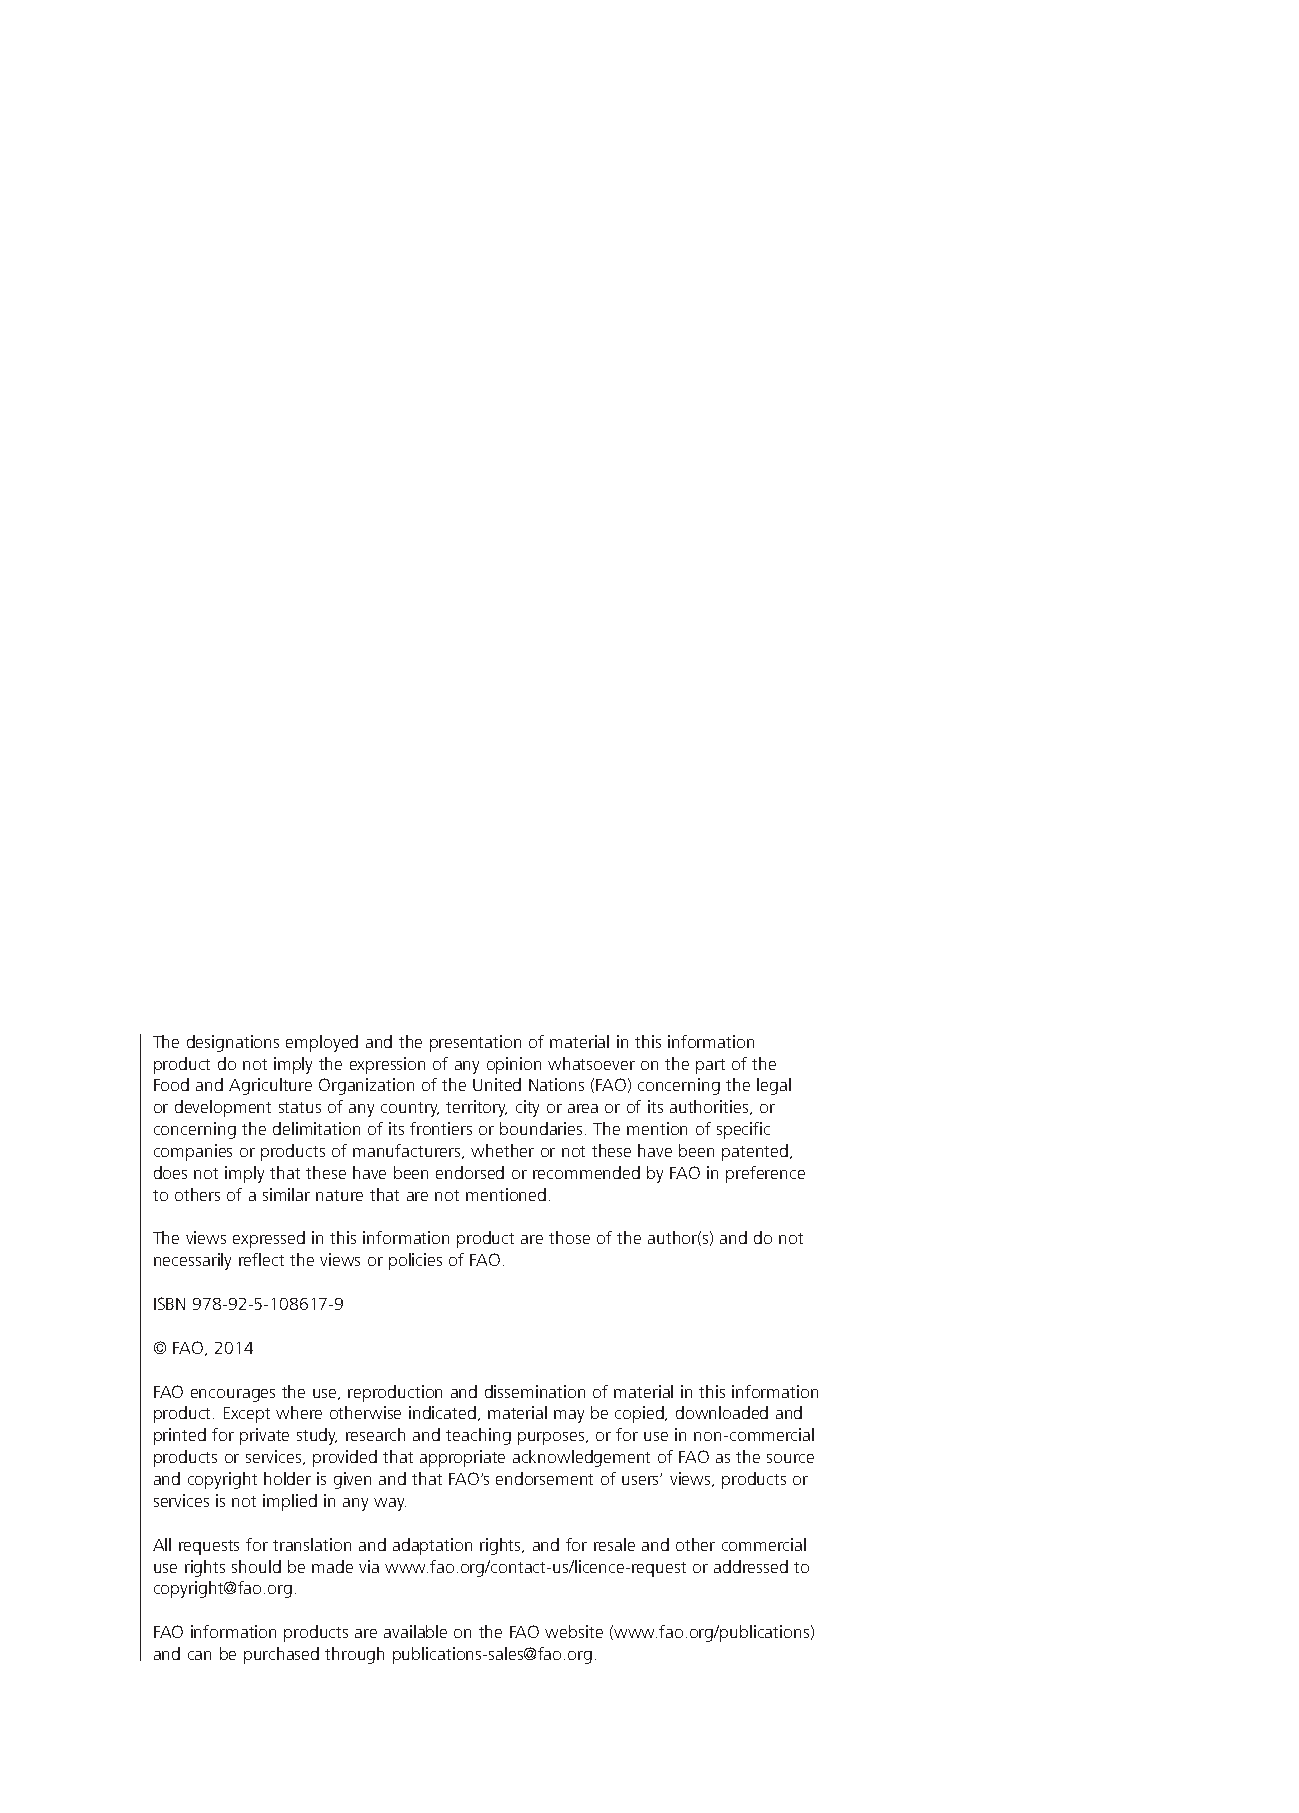
\includepdf[width=\paperwidth,height=\paperheight, offset=-30 -100]{./GSPB15disclamerPage.pdf}
\else
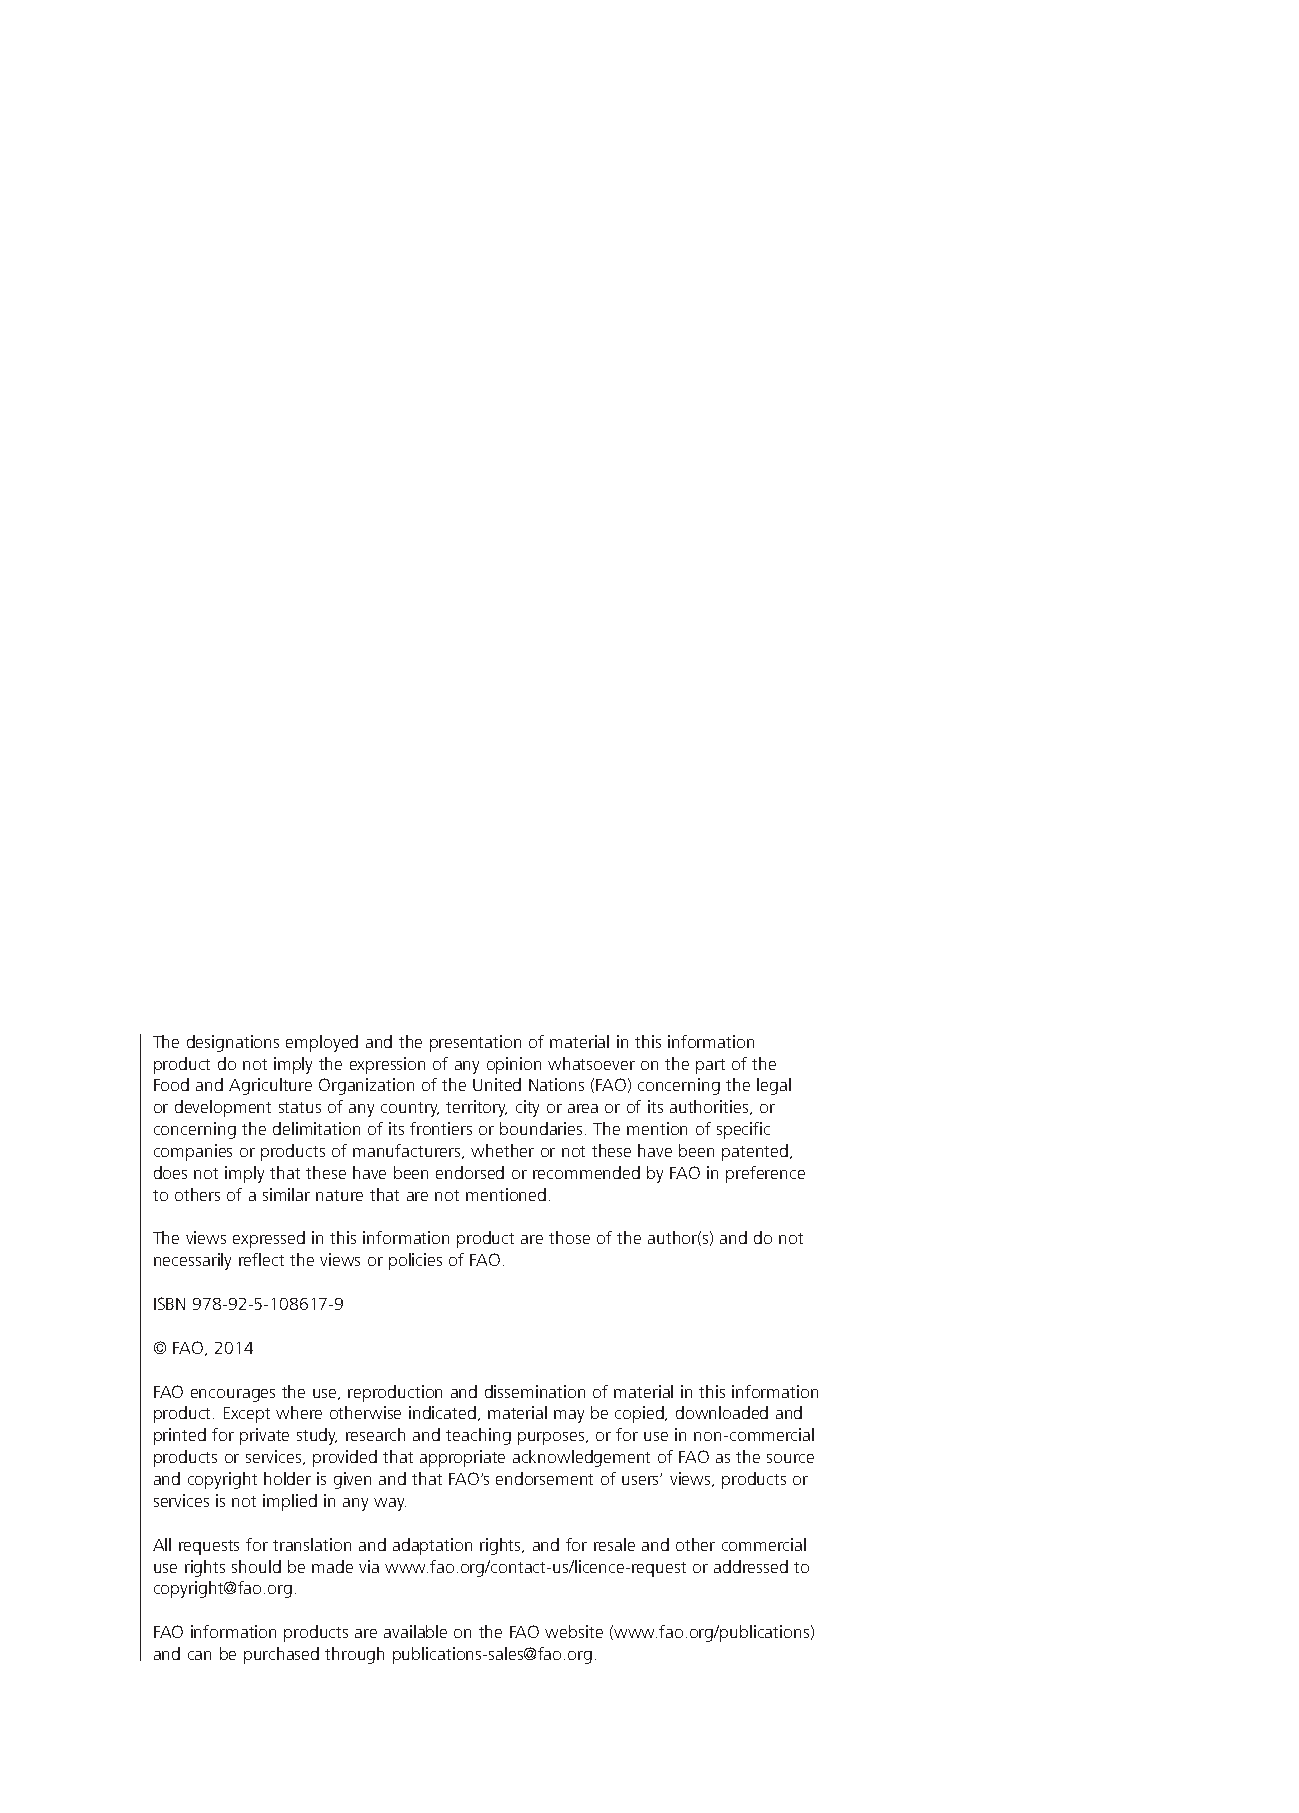
\includepdf[width=\paperwidth,height=\paperheight, offset=-10 -50]{./GSPB15disclamerPage.pdf}
\fi

%% Prelims
\tableofcontents
\clearpage

% Asetetaan koko raportin laajuiset parametrit knitr:lle



%% List of countries
%\phantomsection
%\renewcommand{\indexname}{List of countries} 
%\addcontentsline{toc}{section}{List of countries}
%\printindex

%%% List of tables
%\phantomsection
%\addcontentsline{toc}{section}{List of Tables}
%\listoftables

%% To be commented if we want to show the List of countries
\thispagestyle{empty}
\mbox{}
\clearpage

%% New part - Introduction
\newpart{white}
%\addtocounter{page}{1}
%\cleardoublepage
\pagenumbering{arabic}  %% Arabic page numbering
\setlength{\parskip}{3pt plus 3pt minus 1pt}  %% Increasing the spacing in the introduction page


\section{Foreword}

\bigskip
\bigskip

\large



At the first International Conference on Nutrition, held in 1992, global leaders pledged to “act in solidarity to ensure that freedom from hunger becomes a reality.”

Although great progress has been made in reducing the prevalence of hunger, over 800 million people are still unable to meet their daily calorie needs for living healthy lives. About one in nine people go to bed daily on an empty stomach. In cases where food is available, often the quality of the food does not meet micronutrient (vitamin and mineral) needs. More than two billion people continue to suffer from nutritional deficiencies such as vitamin A, iron, zinc and iodine. While the world is grappling with issues of undernutrition, there is also the growing problem of obesity, which now affects around 500 million people. Many countries are facing a triple burden of malnutrition, where undernourishment, micronutrient deficiency and obesity exist in the same community and household. 

ICN2 presents another opportunity for the global community to make a commitment and take action to address this global menace. The two outcome documents of ICN2 - the Rome Declaration and the Framework for Action - will provide the basis for renewed commitment and focused action for addressing malnutrition within the coming decade. Experiences from the Millennium Development Goals indicate that, with a united commitment, we can achieve significant results. We must now move forward with the same determination as we address new global challenges through the Sustainable Development Goals.

Having clear indicators to measure progress is very important. Statistics are a fundamental tool in this process, necessary to identify problems and monitor progress. The better the data, the better policies can be designed to improve nutrition worldwide. Without good data, it is impossible to evaluate or determine the impact of policies, or hold stakeholders accountable for pledges they make. For statistics to effectively inform food and agriculture policies, they need to be accessible and clear to policymakers at global, regional and country levels. This publication presents selected key indicators related to food and nutrition outcomes that stakeholders can use to prioritise their actions.  

This food and nutrition pocketbook was produced jointly by the FAO Statistics and Nutrition Divisions. It is part of the FAO Statistical Yearbook suite of products and is one of the tools that can be used as building blocks for evidence-based policy making. It includes data from FAOSTAT as well as from other partners in the organization and in the international community. 

There are still gaps in the information. We hope that ICN2 will  provide the  forum for discussion on ways to improve the data to better monitor nutrition.

\bigskip

\ \ \ \ \ \ \ \ \ \ \ \ \ \ \ \ \ \ \ \ \ \ \ \ \ \ \ \ \ \ \ \ \ \ \ \ \ \ \ \ \ \ \ \ \ \ \ \ \ \ \ Pietro Gennari

\vspace{-5pt}
\  \ \ \ \ Chief Statistician and Director, Statistics Division

\clearpage


\thispagestyle{empty}
\mbox{}
\newpage
\section{Introduction}

\bigskip
\bigskip

new line

Overcoming malnutrition in all of its forms – caloric undernourishment, micronutrient deficiencies and obesity – requires a combination of interventions in different areas that guarantee the availability of and access to healthy diets. Among the key areas, interventions are required in food systems, public health systems and the provision of safe water and sanitation. This pocketbook not only focuses on indicators of food security and nutritional outcomes but also on the determinants that contribute to healthy lives. 

The pocketbook is structured in two sections: 
\begin{itemize}
\item Thematic spreads related to food security and nutrition, including detailed food consumption data collected from national household budget surveys,
\item Comprehensive country and regional profiles with indicators categorized by anthropometry, nutritional deficiencies, supplementation, dietary energy supplies, preceded by their "setting".
\end{itemize}

\textit{The setting} provides demographic indicators as well as health status indicators based on mortality patterns and the provision of safe water and sanitation. 

\textit{Anthropometry} indicators provide information not only on the prevalence of acute and chronic forms of under-nutrition but also on the prevalence of obesity. Their co-existence is often referred to as the double burden of malnutrition. 

\textit{Nutritional deficiency} indicators reveal food security issues at the national level based on the adequacy of energy supplies; they also reveal the prevalence of micronutrient deficiencies, often referred to as “hidden hunger”. Combined with anthropometric measurements, they allow for the identification of the triple burden of malnutrition (under-nutrition, obesity and hidden hunger). Regarding hidden hunger, indicators concerning iodine and vitamin A have been selected.

\textit{Dietary} indicators are based on national food supplies and inform on the overall quality of diets. Focus is also on the importance of diets during the first 1\,000 days of an infant’s life, with indicators selected on the quality of breastfeeding, dietary diversity and meal frequency. 

The choice of indicators was guided by the following criteria: relevance to health, food security and nutrition, comparability over time, and availability, in particular for low-income countries. But the criteria were relaxed for several indicators given their importance and the lack of available substitutes. It is hoped that the presence of data gaps will bring about greater efforts to collect the necessary information because only with timely and reliable data can interventions be designed and targeted towards those in most need. Wherever available, disaggregated data by gender have been provided. Such data are indeed key to mainstreaming gender in policies and programmes.

\setlength{\parskip}{0pt}  %% Restoring the normal spacing

\normalsize

\makeatletter\clearpage\ifodd\c@page\hbox{}\newpage\fi\makeatother %% Remove the colored strip from the introduction page

% %%%%%%%%%%%%%%%%%%%%%%%%%%%%%%%%%%%%%%%%%%%%%%%%%%
%% ICN2 pocketbook environments
%%%%%%%%%%%%%%%%%%%%%%%%%%%%%%%%%%%%%%%%%%%%%%%%%%




%%%%%%%%%%%%%%%%%%%%%%%%%%%%%%%%%%%%%%%%%%%%%%%%%%
%% PART1 - The Setting
%%%%%%%%%%%%%%%%%%%%%%%%%%%%%%%%%%%%%%%%%%%%%%%%%%

\newpart{part1}
\rowcolors{1}{part1!10}{white}
\clearpage

%% Economy %%%%%%%%%%%%%%%%%%%%%%%%%%%%%%%%%%%%%%%%%%%

\begin{knitrout}
\definecolor{shadecolor}{rgb}{0.969, 0.969, 0.969}\color{fgcolor}\begin{kframe}
\begin{alltt}
\hlkwd{chart_spread}\hlstd{(}\hlkwc{title}\hlstd{=}\hlstr{"Economy"}\hlstd{,}                \hlcom{# Amy you could specify here}
            \hlkwc{LeftTextCode}\hlstd{=}\hlstr{"TXT.P1.ECON.1.1"}\hlstd{,}  \hlcom{# Amy you could specify here}
            \hlkwc{RightTextCode}\hlstd{=}\hlstr{"C.P1.ECON.1.2"}\hlstd{,}   \hlcom{# Amy you could specify here}
            \hlkwc{LeftChartCode}\hlstd{=}\hlstr{"C.P1.ECON.1.3"}\hlstd{,}   \hlcom{# Amy you could specify here}
            \hlkwc{RightChartCode}\hlstd{=}\hlstr{"C.P1.ECON.1.4"}\hlstd{,}  \hlcom{# Amy you could specify here}
            \hlkwc{BottomChartCode}\hlstd{=}\hlstr{"C.P1.ECON.1.5"}\hlstd{,} \hlcom{# Amy you could specify here}
            \hlkwc{MapCode}\hlstd{=}\hlstr{"M.P1.ECON.1.6"}\hlstd{)}         \hlcom{# Amy you could specify here}
\end{alltt}
\end{kframe}
\end{knitrout}

%% Population %%%%%%%%%%%%%%%%%%%%%%%%%%%%%%%%%%%%%%%%%%%

\begin{knitrout}
\definecolor{shadecolor}{rgb}{0.969, 0.969, 0.969}\color{fgcolor}\begin{kframe}
\begin{alltt}
\hlkwd{chart_spread}\hlstd{(}\hlkwc{title}\hlstd{=}\hlstr{"Population"}\hlstd{,}                               \hlcom{# Amy you could specify here}
            \hlkwc{LeftTextCode}\hlstd{=}\hlstr{"P1.OVER.1.1"}\hlstd{,}                        \hlcom{# Amy you could specify here}
            \hlkwc{RightTextCode}\hlstd{=}\hlstr{"MT.P1.OVER.1.2"}\hlstd{,}                    \hlcom{# Amy you could specify here}
            \hlkwc{footnoteRight}\hlstd{=}\hlstr{"Data after 2010 are projections."}\hlstd{,}  \hlcom{# Amy you could specify here}
            \hlkwc{LeftChartCode}\hlstd{=}\hlstr{"C.P1.OVER.1.2"}\hlstd{,}                     \hlcom{# Amy you could specify here}
            \hlkwc{RightChartCode}\hlstd{=}\hlstr{"C.P1.OVER.1.3"}\hlstd{,}                    \hlcom{# Amy you could specify here}
            \hlkwc{BottomChartCode}\hlstd{=}\hlstr{"C.P1.OVER.1.4"}\hlstd{,}                   \hlcom{# Amy you could specify here}
            \hlkwc{MapCode}\hlstd{=}\hlstr{"M.P1.OVER.1.6"}\hlstd{)}                           \hlcom{# Amy you could specify here}
\end{alltt}
\end{kframe}
\end{knitrout}


%%%%%%%%%%%%%%%%%%%%%%%%%%%%%%%%%%%%%%%%%%%%%%%%%%
%% PART2 - Hunger dimensions
%%%%%%%%%%%%%%%%%%%%%%%%%%%%%%%%%%%%%%%%%%%%%%%%%%

\newpart{part2}
\rowcolors{1}{part1!10}{white}
\clearpage


%% Undernourishment  %%%%%%%%%%%%%%%%%%%%%%%%%%%%%%%%%%%%%%%%%%%

\begin{kframe}
\begin{alltt}
\hlkwd{chart_spread}\hlstd{(}\hlkwc{title}\hlstd{=}\hlstr{"Undernourishment"}\hlstd{,}                \hlcom{# Amy you could specify here}
            \hlkwc{LeftTextCode}\hlstd{=}\hlstr{"TXT.P1.IAF.1.1"}\hlstd{,}  \hlcom{# Amy you could specify here}
            \hlkwc{RightTextCode}\hlstd{=}\hlstr{"MT.P1.IAF.1.2"}\hlstd{,}   \hlcom{# Amy you could specify here}
            \hlkwc{LeftChartCode}\hlstd{=}\hlstr{"C.P1.IAF.1.3"}\hlstd{,}   \hlcom{# Amy you could specify here}
            \hlkwc{RightChartCode}\hlstd{=}\hlstr{"C.P1.IAF.1.4"}\hlstd{,}  \hlcom{# Amy you could specify here}
            \hlkwc{BottomChartCode}\hlstd{=}\hlstr{"C.P1.IAF.1.5"}\hlstd{,} \hlcom{# Amy you could specify here}
            \hlkwc{MapCode}\hlstd{=}\hlstr{"M.P1.IAF.1.6"}\hlstd{)}         \hlcom{# Amy you could specify here}
\end{alltt}
\end{kframe}\begin{ChartPage}{ Undernourishment } 
\LeftText{\IfFileExists{./Text/TXT.P1.IAF.1.1.tex}{Undernourishment refers to food intake that is insufficient to meet dietary energy requirements for an active and healthy life. About 805 million people are estimated to be chronically undernourished in 2012–14. This number has fallen by 100 million over the last decade, and by 209 million since 1990-92. Despite progress, the number is still high, and marked differences across regions persist. Latin America and the Caribbean have made the greatest overall progress, with modest progress in sub-Saharan Africa and Western Asia, which have been afflicted by natural disasters and conflict.}{\lipsum[2]}} 
\RightText{\IfFileExists{./Plots/MT.P1.IAF.1.2.tex} 
 
	               {\begin{table} 

	               \caption{Prevalence of undernourishment (percent, 1990-92 and 2012-14)} 

	               \footnotesize
\begin{center}
\begin{tabular}{lrr}
\toprule
  & 1990-92 & 2012-14\\
\midrule
World & 18.7 & 11.3\\
Developing
countries & 23.4 & 13.5\\
Africa & 27.7 & 20.5\\
Asia & 23.7 & 12.7\\
Latin Am. and the Carib. & 15.3 & 6.1\\
Oceania & 15.7 & 14\\
Developed
countries & $<$5.0 & $<$5.0\\
\toprule
\end{tabular}
\end{center}
 
\footnotesize{}  
 

	               \end{table}}} 
 
\LeftChart{\begin{chart} 
 
	               \caption{Asian countries with the highest number of people undernourished in 2012-14 (1990-92 and 2012-14)} 
\IfFileExists{./Plots/C.P1.IAF.1.3.pdf}{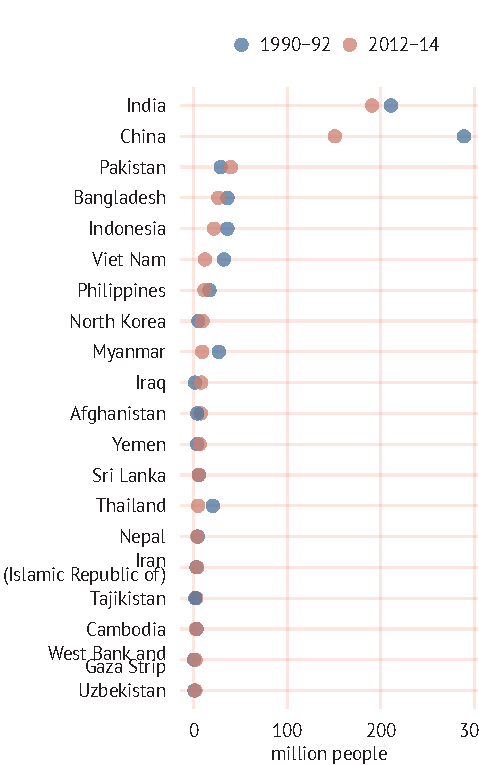
\includegraphics[width = 4cm, height = 8cm]{{./Plots/C.P1.IAF.1.3}.pdf}}{} 
\end{chart}} 
\RightChart{\begin{chart} 
 
	               \caption{African countries with the highest number of people undernourished in 2012-14 (1990-92 and 2012-14)} 
\vspace{-7pt} 
\IfFileExists{./Plots/C.P1.IAF.1.4.pdf}{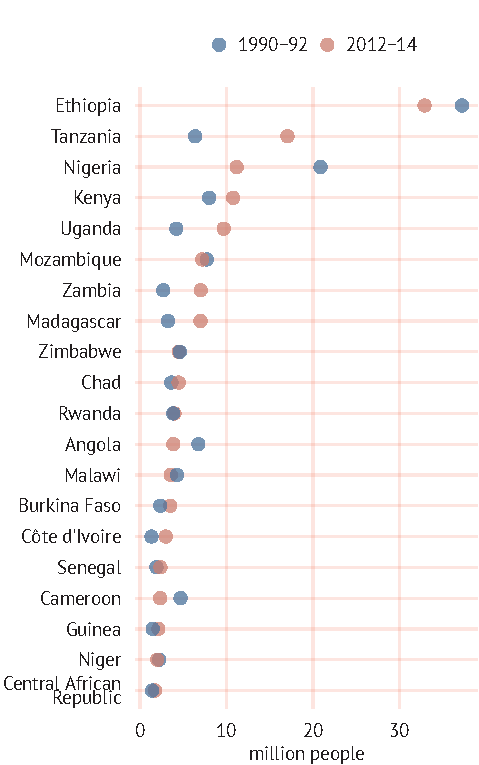
\includegraphics[width = 4cm, height = 8cm]{{./Plots/C.P1.IAF.1.4}.pdf}}{} 
\end{chart}} 
\BottomChart{\begin{chart} 
 
	               \caption{Number of people undernourished (1990-92 to 2012-14)} 
\vspace{-7pt} 
\IfFileExists{./Plots/C.P1.IAF.1.5.pdf}{
\includegraphics[width = 8cm, height = 3cm]{{./Plots/C.P1.IAF.1.5}.pdf}}{} 
\end{chart}} 
\end{ChartPage}\begin{figure} 
\caption{Prevalence of people undernourished (percent, 2014)} 
\IfFileExists{./Maps/M.P1.IAF.1.6.pdf}{\centering
\includegraphics[height = 1\columnwidth, angle=90]{{./Maps/M.P1.IAF.1.6}.pdf}\par}{\newpage\thispagestyle{empty}\mbox{}}{} 
\end{figure}



%%%%%%%%%%%%%%%%%%%%%%%%%%%%%%%%%%%%%%%%%%%%%%%%%%
%% PART3 - Food Supply
%%%%%%%%%%%%%%%%%%%%%%%%%%%%%%%%%%%%%%%%%%%%%%%%%%

\newpart{part3}
\rowcolors{1}{part1!10}{white}
\clearpage


%% Production %%%%%%%%%%%%%%%%%%%%%%%%%%%%%%%%%%%%%%%%%%%

\begin{knitrout}
\definecolor{shadecolor}{rgb}{0.969, 0.969, 0.969}\color{fgcolor}\begin{kframe}
\begin{alltt}
\hlkwd{chart_spread}\hlstd{(}\hlkwc{title}\hlstd{=}\hlstr{"Production"}\hlstd{,}             \hlcom{# Amy you could specify here}
            \hlkwc{LeftTextCode}\hlstd{=}\hlstr{"TXT.P1.ECON.1.1"}\hlstd{,}  \hlcom{# Amy you could specify here}
            \hlkwc{RightTextCode}\hlstd{=}\hlstr{"C.P1.ECON.1.2"}\hlstd{,}   \hlcom{# Amy you could specify here}
            \hlkwc{LeftChartCode}\hlstd{=}\hlstr{"C.P1.ECON.1.3"}\hlstd{,}   \hlcom{# Amy you could specify here}
            \hlkwc{RightChartCode}\hlstd{=}\hlstr{"C.P1.ECON.1.4"}\hlstd{,}  \hlcom{# Amy you could specify here}
            \hlkwc{BottomChartCode}\hlstd{=}\hlstr{"C.P1.ECON.1.5"}\hlstd{,} \hlcom{# Amy you could specify here}
            \hlkwc{MapCode}\hlstd{=}\hlstr{"M.P1.ECON.1.6"}\hlstd{)}         \hlcom{# Amy you could specify here}
\end{alltt}
\end{kframe}
\end{knitrout}


%%%%%%%%%%%%%%%%%%%%%%%%%%%%%%%%%%%%%%%%%%%%%%%%%%
%% PART4 - Sustainability dimensions
%%%%%%%%%%%%%%%%%%%%%%%%%%%%%%%%%%%%%%%%%%%%%%%%%%

\newpart{part2}
\rowcolors{1}{part1!10}{white}
\clearpage

%% Forests %%%%%%%%%%%%%%%%%%%%%%%%%%%%%%%%%%%%%%%%%%%

\begin{knitrout}
\definecolor{shadecolor}{rgb}{0.969, 0.969, 0.969}\color{fgcolor}\begin{kframe}
\begin{alltt}
\hlkwd{chart_spread}\hlstd{(}\hlkwc{title}\hlstd{=}\hlstr{"Forests"}\hlstd{,}                \hlcom{# Amy you could specify here}
            \hlkwc{LeftTextCode}\hlstd{=}\hlstr{"TXT.P1.ECON.1.1"}\hlstd{,}  \hlcom{# Amy you could specify here}
            \hlkwc{RightTextCode}\hlstd{=}\hlstr{"C.P1.ECON.1.2"}\hlstd{,}   \hlcom{# Amy you could specify here}
            \hlkwc{LeftChartCode}\hlstd{=}\hlstr{"C.P1.ECON.1.3"}\hlstd{,}   \hlcom{# Amy you could specify here}
            \hlkwc{RightChartCode}\hlstd{=}\hlstr{"C.P1.ECON.1.4"}\hlstd{,}  \hlcom{# Amy you could specify here}
            \hlkwc{BottomChartCode}\hlstd{=}\hlstr{"C.P1.ECON.1.5"}\hlstd{,} \hlcom{# Amy you could specify here}
            \hlkwc{MapCode}\hlstd{=}\hlstr{"M.P1.ECON.1.6"}\hlstd{)}         \hlcom{# Amy you could specify here}
\end{alltt}
\end{kframe}
\end{knitrout}




%%%%%%%%%%%%%%%%%%%%%%%%%%%%%%%%%%%%%%%%%%%%%%%%%%
%% ICN2 pocketbook environments
%%%%%%%%%%%%%%%%%%%%%%%%%%%%%%%%%%%%%%%%%%%%%%%%%%




%%%%%%%%%%%%%%%%%%%%%%%%%%%%%%%%%%%%%%%%%%%%%%%%%%
%% PART1 - The Setting
%%%%%%%%%%%%%%%%%%%%%%%%%%%%%%%%%%%%%%%%%%%%%%%%%%

\newpart{part1}
\rowcolors{1}{part1!10}{white}
\clearpage

%% Economy %%%%%%%%%%%%%%%%%%%%%%%%%%%%%%%%%%%%%%%%%%%



%% Population %%%%%%%%%%%%%%%%%%%%%%%%%%%%%%%%%%%%%%%%%%%




%%%%%%%%%%%%%%%%%%%%%%%%%%%%%%%%%%%%%%%%%%%%%%%%%%
%% PART2 - Hunger dimensions
%%%%%%%%%%%%%%%%%%%%%%%%%%%%%%%%%%%%%%%%%%%%%%%%%%

\newpart{part2}
\rowcolors{1}{part1!10}{white}
\clearpage


%% Undernourishment  %%%%%%%%%%%%%%%%%%%%%%%%%%%%%%%%%%%%%%%%%%%

\begin{ChartPage}{ Undernourishment } 
\LeftText{\IfFileExists{./Text/TXT.P1.IAF.1.1.tex}{Undernourishment refers to food intake that is insufficient to meet dietary energy requirements for an active and healthy life. About 805 million people are estimated to be chronically undernourished in 2012–14. This number has fallen by 100 million over the last decade, and by 209 million since 1990-92. Despite progress, the number is still high, and marked differences across regions persist. Latin America and the Caribbean have made the greatest overall progress, with modest progress in sub-Saharan Africa and Western Asia, which have been afflicted by natural disasters and conflict.}{\lipsum[2]}} 
\RightText{\IfFileExists{./Tables/MT.P1.IAF.1.2.tex}  
	               {\begin{table} 

	               \caption{Prevalence of undernourishment (percent, 1990-92 and 2012-14)} 

	               \footnotesize
\begin{center}
\begin{tabular}{lrr}
\toprule
  & 1990-92 & 2012-14\\
\midrule
World & 18.7 & 11.3\\
Developing
countries & 23.4 & 13.5\\
Africa & 27.7 & 20.5\\
Asia & 23.7 & 12.7\\
Latin Am. and the Carib. & 15.3 & 6.1\\
Oceania & 15.7 & 14\\
Developed
countries & $<$5.0 & $<$5.0\\
\toprule
\end{tabular}
\end{center}
 

	               \end{table}}} 
 
\LeftChart{\begin{chart} 
 
	               \caption{Asian countries with the highest number of people undernourished in 2012-14 (1990-92 and 2012-14)} 
\footnotesize{}  
\IfFileExists{./Plots/C.P1.IAF.1.3.pdf}{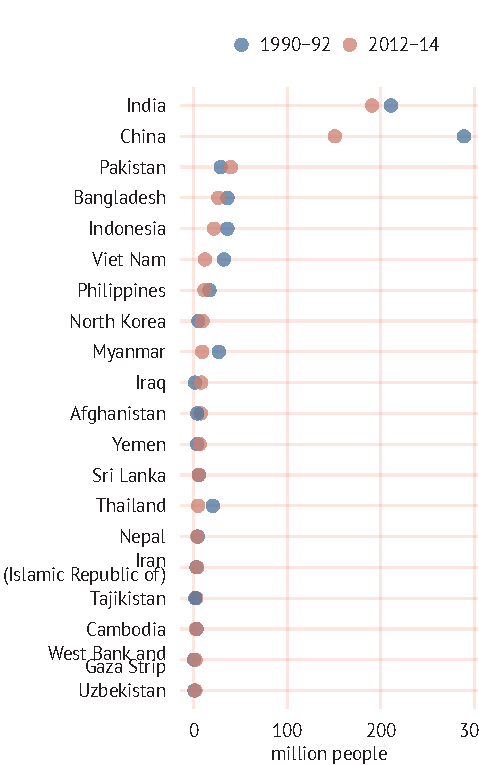
\includegraphics[width = 4.5cm, height = 6.5cm]{{./Plots/C.P1.IAF.1.3}.pdf}}{} 
\end{chart}} 
\RightChart{\begin{chart} 
 
	               \caption{African countries with the highest number of people undernourished in 2012-14 (1990-92 and 2012-14)} 
\footnotesize{}  
\IfFileExists{./Plots/C.P1.IAF.1.4.pdf}{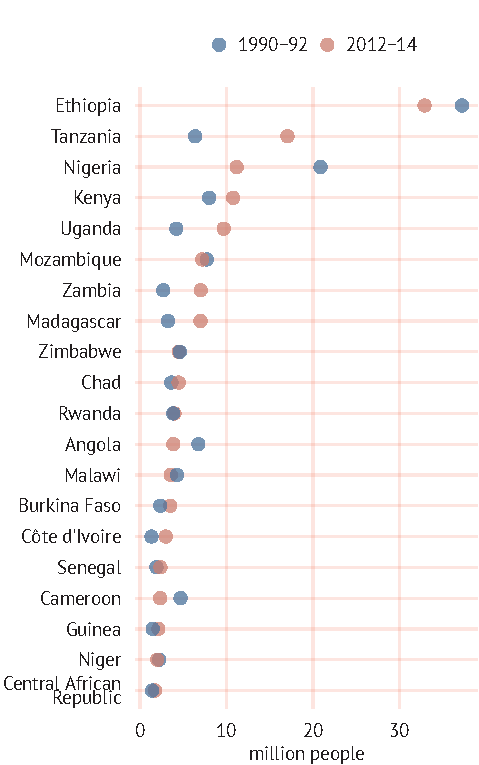
\includegraphics[width = 4.5cm, height = 6.5cm]{{./Plots/C.P1.IAF.1.4}.pdf}}{} 
\end{chart}} 
\BottomChart{\begin{chart} 
 
	               \caption{Number of people undernourished (1990-92 to 2012-14)} 
\IfFileExists{./Plots/C.P1.IAF.1.5.pdf}{
\includegraphics[width = 8cm, height = 3.5cm]{{./Plots/C.P1.IAF.1.5}.pdf}}{} 
\end{chart}} 
\end{ChartPage}\begin{figure} 
\caption{Prevalence of people undernourished (percent, 2014)} 
\IfFileExists{./Maps/M.P1.IAF.1.6.pdf}{\centering
\includegraphics[height = 1\columnwidth, angle=90]{{./Maps/M.P1.IAF.1.6}.pdf}\par}{\newpage\thispagestyle{empty}\mbox{}}{} 
\end{figure}



\begin{ChartPage}{ Undernourishment2 } 
\LeftText{\IfFileExists{./Text/TXT.P1.IAF.1.1.tex}{Undernourishment refers to food intake that is insufficient to meet dietary energy requirements for an active and healthy life. About 805 million people are estimated to be chronically undernourished in 2012–14. This number has fallen by 100 million over the last decade, and by 209 million since 1990-92. Despite progress, the number is still high, and marked differences across regions persist. Latin America and the Caribbean have made the greatest overall progress, with modest progress in sub-Saharan Africa and Western Asia, which have been afflicted by natural disasters and conflict.}{\lipsum[2]}} 
\RightText{\IfFileExists{./Tables/MT.P1.IAF.1.2.tex}  
	               {\begin{table} 

	               \caption{Prevalence of undernourishment (percent, 1990-92 and 2012-14)} 

	               \footnotesize
\begin{center}
\begin{tabular}{lrr}
\toprule
  & 1990-92 & 2012-14\\
\midrule
World & 18.7 & 11.3\\
Developing
countries & 23.4 & 13.5\\
Africa & 27.7 & 20.5\\
Asia & 23.7 & 12.7\\
Latin Am. and the Carib. & 15.3 & 6.1\\
Oceania & 15.7 & 14\\
Developed
countries & $<$5.0 & $<$5.0\\
\toprule
\end{tabular}
\end{center}
 

	               \end{table}}} 
 
\LeftChart{\begin{chart} 
 
	               \caption{Asian countries with the highest number of people undernourished in 2012-14 (1990-92 and 2012-14)} 
\footnotesize{}  
\IfFileExists{./Plots/C.P1.IAF.1.3.pdf}{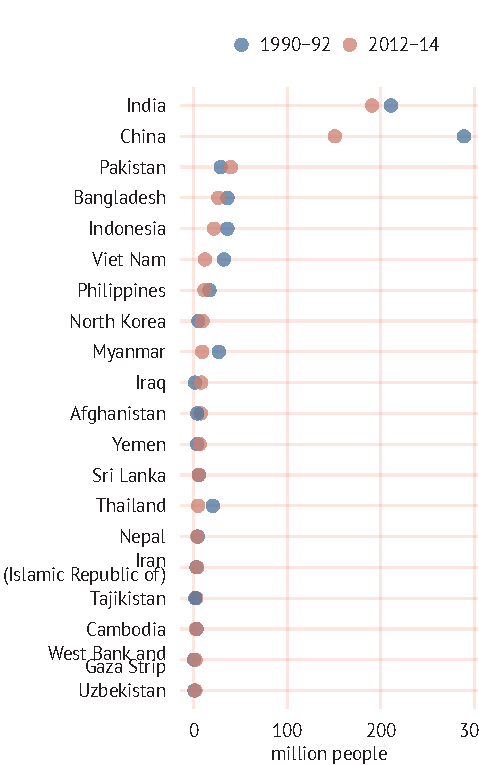
\includegraphics[width = 4.5cm, height = 6.5cm]{{./Plots/C.P1.IAF.1.3}.pdf}}{} 
\end{chart}} 
\RightChart{\begin{chart} 
 
	               \caption{African countries with the highest number of people undernourished in 2012-14 (1990-92 and 2012-14)} 
\footnotesize{}  
\IfFileExists{./Plots/C.P1.IAF.1.4.pdf}{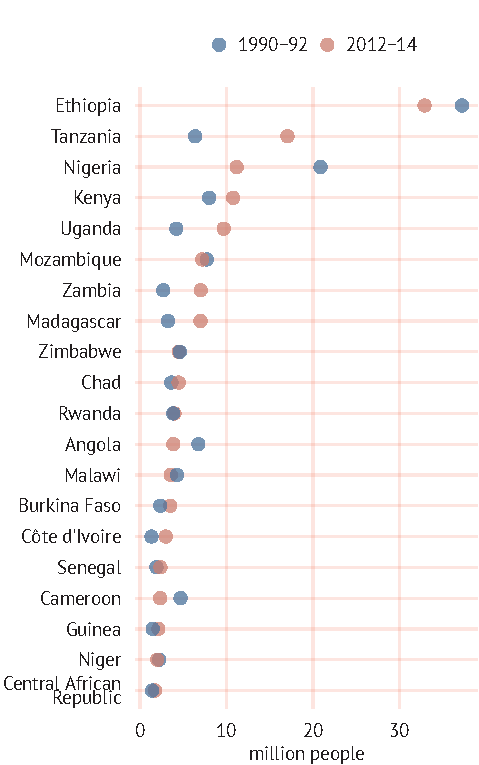
\includegraphics[width = 4.5cm, height = 6.5cm]{{./Plots/C.P1.IAF.1.4}.pdf}}{} 
\end{chart}} 
\BottomChart{\begin{chart} 
 
	               \caption{Number of people undernourished (1990-92 to 2012-14)} 
\IfFileExists{./Plots/C.P1.IAF.1.5.pdf}{
\includegraphics[width = 8cm, height = 3.5cm]{{./Plots/C.P1.IAF.1.5}.pdf}}{} 
\end{chart}} 
\end{ChartPage}\begin{figure} 
\caption{Prevalence of people undernourished (percent, 2014)} 
\IfFileExists{./Maps/M.P1.IAF.1.7.pdf}{\centering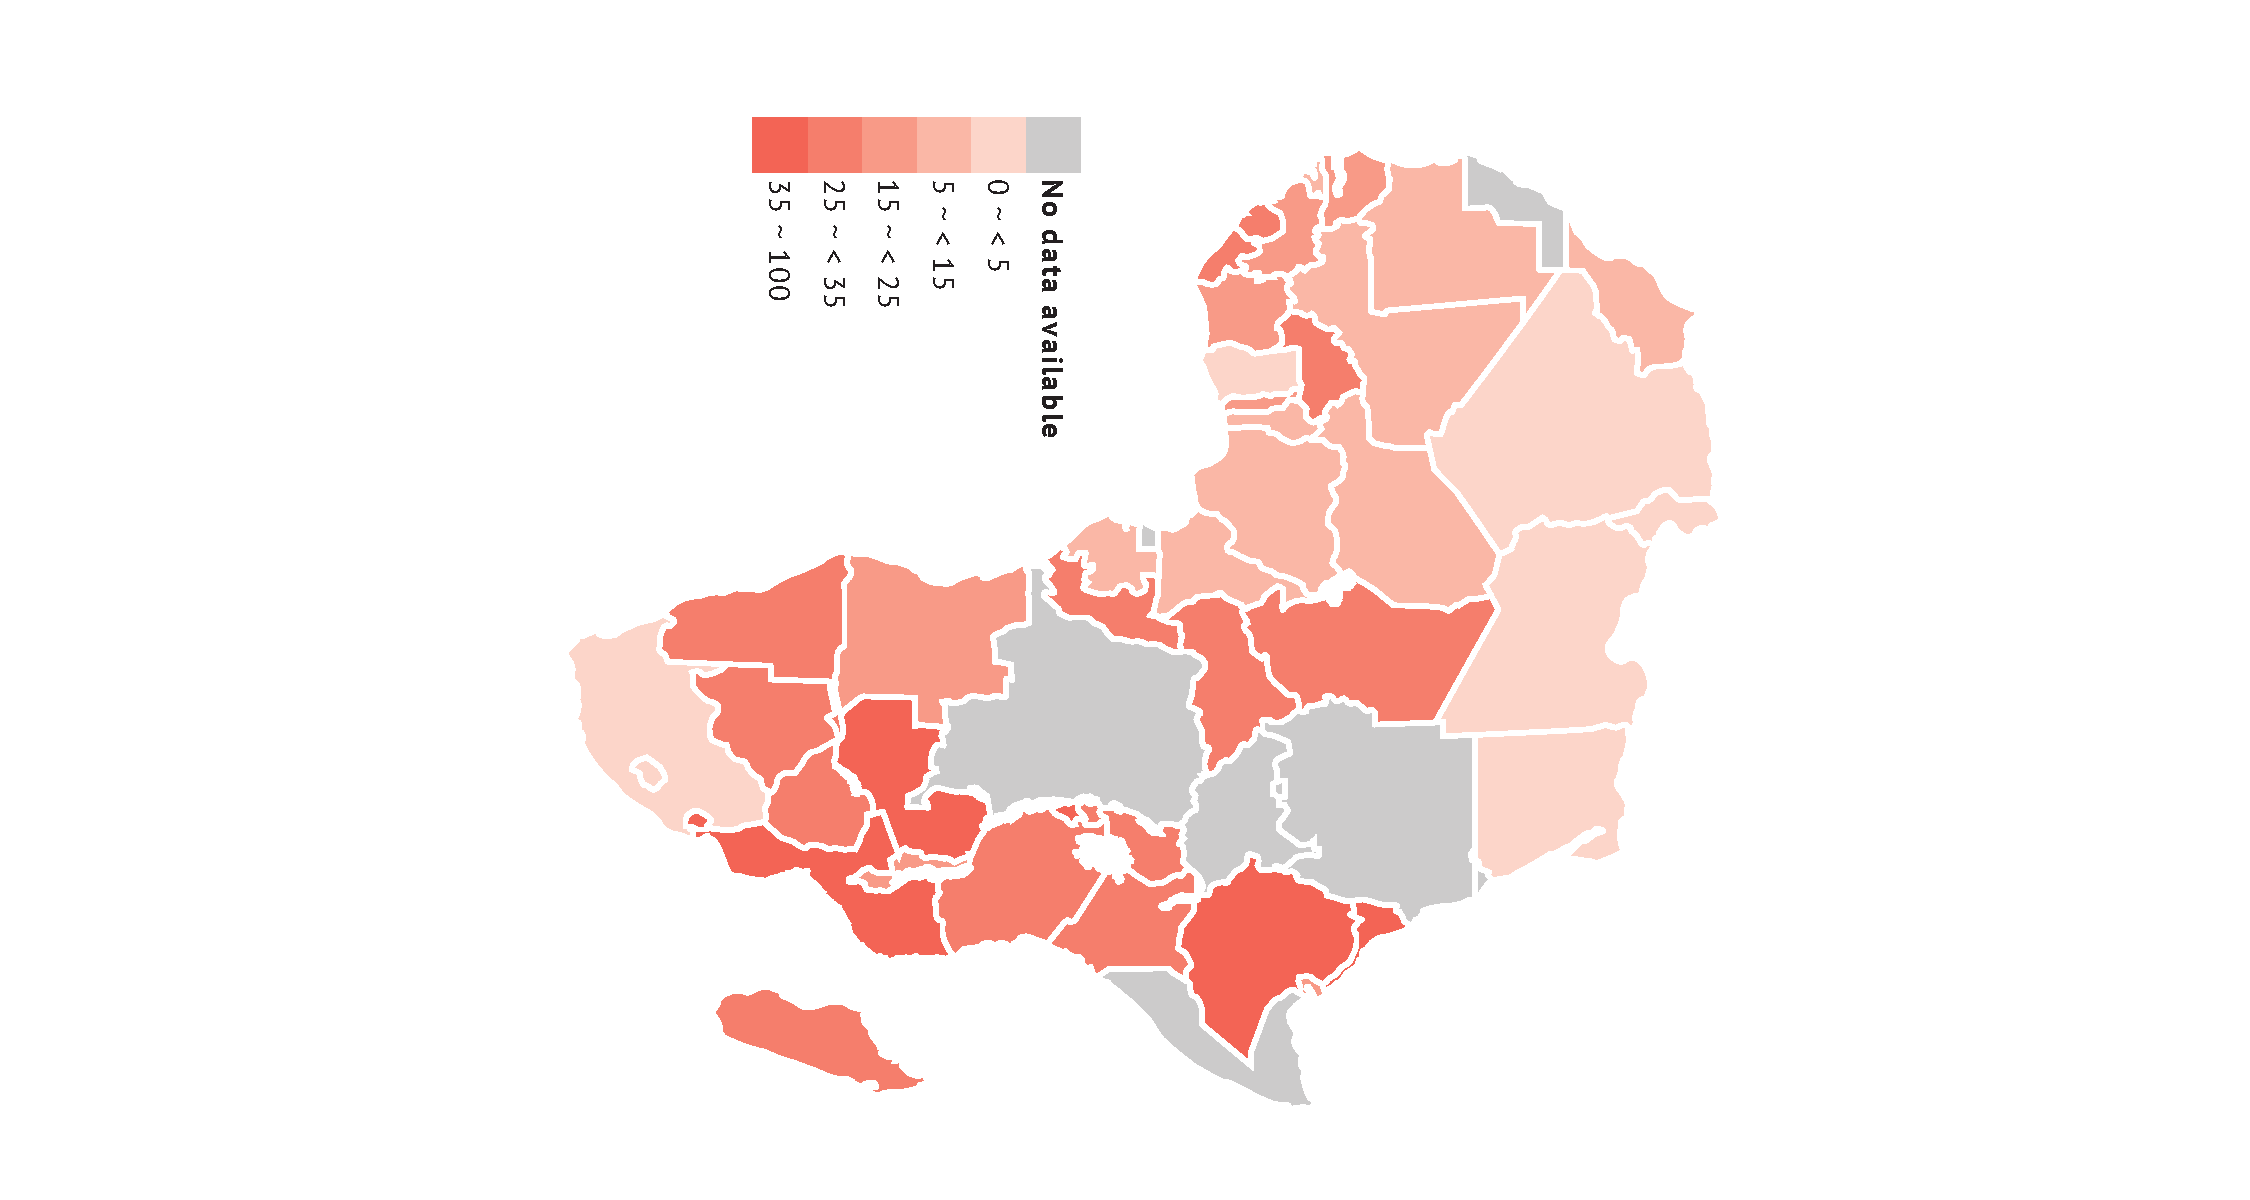
\includegraphics[height = 1\columnwidth, angle=90]{{./Maps/M.P1.IAF.1.7}.pdf}\par}{\newpage\thispagestyle{empty}\mbox{}}{} 
\end{figure}


%%%%%%%%%%%%%%%%%%%%%%%%%%%%%%%%%%%%%%%%%%%%%%%%%%
%% PART3 - Food Supply
%%%%%%%%%%%%%%%%%%%%%%%%%%%%%%%%%%%%%%%%%%%%%%%%%%

\newpart{part3}
\rowcolors{1}{part1!10}{white}
\clearpage


%% Production %%%%%%%%%%%%%%%%%%%%%%%%%%%%%%%%%%%%%%%%%%%




%%%%%%%%%%%%%%%%%%%%%%%%%%%%%%%%%%%%%%%%%%%%%%%%%%
%% PART4 - Sustainability dimensions
%%%%%%%%%%%%%%%%%%%%%%%%%%%%%%%%%%%%%%%%%%%%%%%%%%

\newpart{part2}
\rowcolors{1}{part1!10}{white}
\clearpage

%% Forests %%%%%%%%%%%%%%%%%%%%%%%%%%%%%%%%%%%%%%%%%%%





% \newpage
% \pagecolor{FAOblue}
% \thispagestyle{empty}
% \mbox{}
% \newpage
% \thispagestyle{empty}
% \mbox{}
% \clearpage
% \pagecolor{white}

%%% COUNTRY DATA
\newpart{FAOblue}
\phantomsection
\addcontentsline{toc}{section}{Country Profiles}
\faoset{bgcolor=white}\selectcolor
\parindent=0pt
\parskip=\medskipamount
\hangafter=-2
\renewcommand{\arraystretch}{1.1}
\setlength{\tabcolsep}{4pt}
\normalsize
\CountryData{ World }
      \rowcolors{1}{FAOblue!10}{white}
      \begin{tabular}{L{3.9cm} R{1cm} R{1cm} R{1cm}}
      \toprule
      \multicolumn{1}{c}{} & \multicolumn{1}{c}{ 1992 } & \multicolumn{1}{c}{ 2002 } & \multicolumn{1}{c}{ 2014 } \\
      \midrule
	\multicolumn{4}{l}{\textcolor{FAOblue}{\textbf{\large{The setting}}}} \\ 
	 ~ Total population (mln) &  ~ \ \ &  ~ \ \ &  ~ \ \ \\ 
	 ~ Average total population growth (\%) &  ~ \ \ &  ~ \ \ &  ~ \ \ \\ 
	 ~ Rural population (\% total population) &  ~ \ \ &  ~ \ \ &  ~ \ \ \\ 
	 ~ Public agricultural expenditure (\% total pub. expenditure) &  ~ \ \ &  ~ \ \ &  ~ \ \ \\ 
	 ~ Area Harvested (ha) &  ~ \ \ &  ~ \ \ &  ~ \ \ \\ 
	 ~ Cropping Intensity Ratio (\%) &  ~ \ \ &  ~ \ \ &  ~ \ \ \\ 
	 ~ Water resources (m\textsuperscript{3}person) &  ~ \ \ &  ~ \ \ &  ~ \ \ \\ 
	 ~ Area equipped for irrigation (\%) &  ~ \ \ &  ~ \ \ &  ~ \ \ \\ 
	 ~ Area Irrigated (ha) &  ~ \ \ &  ~ \ \ &  ~ \ \ \\ 
	 ~ Employment in agriculture (\%) &  ~ \ \ &  ~ \ \ &  ~ \ \ \\ 
	 ~ Employment in agriculture, female (\%) &  ~ \ \ &  ~ \ \ &  ~ \ \ \\ 
	 ~ Total Fertilizers N/P/K (tonnes/ha) &  ~ \ \ &  ~ \ \ &  ~ \ \ \\ 
	 ~ Nitrogen (tonnes/ha) &  ~ \ \ &  ~ \ \ &  ~ \ \ \\ 
	 ~ Energy use intensity in agriculture (mj/I\$) &  ~ \ \ &  ~ \ \ &  ~ \ \ \\ 
	 ~ Shares of farms, $<$2 ha (\%) &  ~ \ \ &  ~ \ \ &  ~ \ \ \\ 
	 ~ Poverty headcount ratios for farm household populations (\%) &  ~ \ \ &  ~ \ \ &  ~ \ \ \\ 
	 ~ Average Farm Size (ha) &  ~ \ \ &  ~ \ \ &  ~ \ \ \\ 
	 ~ Agricultural production operated by the smallest 75 percent of family farms (\%) &  ~ \ \ &  ~ \ \ &  ~ \ \ \\ 
	 ~ Agricultural land operated by the smallest 75 percent of family farms (\%) &  ~ \ \ &  ~ \ \ &  ~ \ \ \\ 
	 ~ Intensity of fertilizer use, by farm size (PPP dollars) &  ~ \ \ &  ~ \ \ &  ~ \ \ \\ 
	 ~ Land productivity, by farm size (Constant 2009 PPP dollars) &  ~ \ \ &  ~ \ \ &  ~ \ \ \\ 
	 ~ Agr. value added per worker (const. 2000 US\$) &  ~ \ \ &  ~ \ \ &  ~ \ \ \\ 
	\multicolumn{4}{l}{\textcolor{FAOblue}{\textbf{\large{Hunger dimensions}}}} \\ 
	 ~ GDP /per capita &  ~ \ \ &  ~ \ \ &  ~ \ \ \\ 
	 ~ Prevalence of undernourished &  ~ \ \ &  ~ \ \ &  ~ \ \ \\ 
	 ~ Children $<$5 year underweight (\%) &  ~ \ \ &  ~ \ \ &  ~ \ \ \\ 
	 ~ Dietary energy supply (kcal/pc/day) &  ~ \ \ &  ~ \ \ &  ~ \ \ \\ 
	 ~ Cereal-excluding beer production index (2004-06=100) &  ~ \ \ &  ~ \ \ &  ~ \ \ \\ 
	 ~ Vegetable oils production index (2004-06=100) &  ~ \ \ &  ~ \ \ &  ~ \ \ \\ 
	 ~ Milk - Excluding Butter index (2004-06=100) &  ~ \ \ &  ~ \ \ &  ~ \ \ \\ 
	 ~ Root and tuber production index (2004-06=100) &  ~ \ \ &  ~ \ \ &  ~ \ \ \\ 
	 ~ Vegetable production index (2004-06=100) &  ~ \ \ &  ~ \ \ &  ~ \ \ \\ 
	 ~ Sugar production index (2004-06=100) &  ~ \ \ &  ~ \ \ &  ~ \ \ \\ 
	 ~ Fruit production index (2004-06=100) &  ~ \ \ &  ~ \ \ &  ~ \ \ \\ 
	 ~ Total meat production index (2004-06=100) &  ~ \ \ &  ~ \ \ &  ~ \ \ \\ 
	 ~ Animal product-excluding meat production index (2004-06=100) &  ~ \ \ &  ~ \ \ &  ~ \ \ \\ 
	 ~ Share of energy supply from cereals, roots and tubers (\%) &  ~ \ \ &  ~ \ \ &  ~ \ \ \\ 
	 ~ Change in food CPI &  ~ \ \ &  ~ \ \ &  ~ \ \ \\ 
	 ~ No access to sanitation facilities (\% pop.) &  ~ \ \ &  ~ \ \ &  ~ \ \ \\ 
	 ~ No access to improved water sources (\% pop.) &  ~ \ \ &  ~ \ \ &  ~ \ \ \\ 
	 ~ Domestic food price volatility &  ~ \ \ &  ~ \ \ &  ~ \ \ \\ 
	 ~ Pop. affected by droughts, floods, extr. temp. (\%) &  ~ \ \ &  ~ \ \ &  ~ \ \ \\ 
	\multicolumn{4}{l}{\textcolor{FAOblue}{\textbf{\large{Food Supply}}}} \\ 
	 ~ Growth value of food production (\%) &  ~ \ \ &  ~ \ \ &  ~ \ \ \\ 
	 ~ Value added from agriculture (\% GDP) &  ~ \ \ &  ~ \ \ &  ~ \ \ \\ 
	 ~ Net pc food production index (2004-06=100) &  ~ \ \ &  ~ \ \ &  ~ \ \ \\ 
	 ~ Net pc crop production index (2004-06=100) &  ~ \ \ &  ~ \ \ &  ~ \ \ \\ 
	 ~ Net pc livestock production index (2004-06=100) &  ~ \ \ &  ~ \ \ &  ~ \ \ \\ 
	 ~ Food exports (mln US\$) &  ~ \ \ &  ~ \ \ &  ~ \ \ \\ 
	 ~ Food imports (mln US\$) &  ~ \ \ &  ~ \ \ &  ~ \ \ \\ 
	 ~ Cereal Imports Dependency Ratio &  ~ \ \ &  ~ \ \ &  ~ \ \ \\ 
	 ~ Value of food imports over total merchandise exports (\%) &  ~ \ \ &  ~ \ \ &  ~ \ \ \\ 
	 ~ Net trade of cereals (mln US\$) &  ~ \ \ &  ~ \ \ &  ~ \ \ \\ 
	 ~ Net trade of meat (mln US\$) &  ~ \ \ &  ~ \ \ &  ~ \ \ \\ 
	 ~ Net trade of fruit and veg. (mln US\$) &  ~ \ \ &  ~ \ \ &  ~ \ \ \\ 
	 ~ Net trade of dairy products (mln const. 2005 US\$) &  ~ \ \ &  ~ \ \ &  ~ \ \ \\ 
	\multicolumn{4}{l}{\textcolor{FAOblue}{\textbf{\large{Sustainability dimensions}}}} \\ 
	 ~ Forest area (\%) &  ~ \ \ &  ~ \ \ &  ~ \ \ \\ 
	 ~ Freshwater withdrawn by agriculture (\%) &  ~ \ \ &  ~ \ \ &  ~ \ \ \\ 
	 ~ Terrestrial protected areas (\%) &  ~ \ \ &  ~ \ \ &  ~ \ \ \\ 
	 ~ Organic area (\%) &  ~ \ \ &  ~ \ \ &  ~ \ \ \\ 
	 ~ Share of renewable water resources (\%) &  ~ \ \ &  ~ \ \ &  ~ \ \ \\ 
	 ~ Biofuel production (thousand kt of oil eq.) &  ~ \ \ &  ~ \ \ &  ~ \ \ \\ 
	 ~ Wood pellets prod. (thousand tonnes) &  ~ \ \ &  ~ \ \ &  ~ \ \ \\ 
	 ~ GHG emissions (AFOLU), emissions in CO\textsubscript{2}eq (gigagrams) &  ~ \ \ &  ~ \ \ &  ~ \ \ \\ 
	 ~ GHG emissions (AFOLU)/GHG (all sectors) &  ~ \ \ &  ~ \ \ &  ~ \ \ \\ 
       \toprule
      \end{tabular}
      \clearpage
\CountryData{ Developing regions }
      \rowcolors{1}{FAOblue!10}{white}
      \begin{tabular}{L{3.9cm} R{1cm} R{1cm} R{1cm}}
      \toprule
      \multicolumn{1}{c}{} & \multicolumn{1}{c}{ 1992 } & \multicolumn{1}{c}{ 2002 } & \multicolumn{1}{c}{ 2014 } \\
      \midrule
	\multicolumn{4}{l}{\textcolor{FAOblue}{\textbf{\large{The setting}}}} \\ 
	 ~ Total population (mln) &  ~ \ \ &  ~ \ \ &  ~ \ \ \\ 
	 ~ Average total population growth (\%) &  ~ \ \ &  ~ \ \ &  ~ \ \ \\ 
	 ~ Rural population (\% total population) &  ~ \ \ &  ~ \ \ &  ~ \ \ \\ 
	 ~ Public agricultural expenditure (\% total pub. expenditure) &  ~ \ \ &  ~ \ \ &  ~ \ \ \\ 
	 ~ Area Harvested (ha) &  ~ \ \ &  ~ \ \ &  ~ \ \ \\ 
	 ~ Cropping Intensity Ratio (\%) &  ~ \ \ &  ~ \ \ &  ~ \ \ \\ 
	 ~ Water resources (m\textsuperscript{3}person) &  ~ \ \ &  ~ \ \ &  ~ \ \ \\ 
	 ~ Area equipped for irrigation (\%) &  ~ \ \ &  ~ \ \ &  ~ \ \ \\ 
	 ~ Area Irrigated (ha) &  ~ \ \ &  ~ \ \ &  ~ \ \ \\ 
	 ~ Employment in agriculture (\%) &  ~ \ \ &  ~ \ \ &  ~ \ \ \\ 
	 ~ Employment in agriculture, female (\%) &  ~ \ \ &  ~ \ \ &  ~ \ \ \\ 
	 ~ Total Fertilizers N/P/K (tonnes/ha) &  ~ \ \ &  ~ \ \ &  ~ \ \ \\ 
	 ~ Nitrogen (tonnes/ha) &  ~ \ \ &  ~ \ \ &  ~ \ \ \\ 
	 ~ Energy use intensity in agriculture (mj/I\$) &  ~ \ \ &  ~ \ \ &  ~ \ \ \\ 
	 ~ Shares of farms, $<$2 ha (\%) &  ~ \ \ &  ~ \ \ &  ~ \ \ \\ 
	 ~ Poverty headcount ratios for farm household populations (\%) &  ~ \ \ &  ~ \ \ &  ~ \ \ \\ 
	 ~ Average Farm Size (ha) &  ~ \ \ &  ~ \ \ &  ~ \ \ \\ 
	 ~ Agricultural production operated by the smallest 75 percent of family farms (\%) &  ~ \ \ &  ~ \ \ &  ~ \ \ \\ 
	 ~ Agricultural land operated by the smallest 75 percent of family farms (\%) &  ~ \ \ &  ~ \ \ &  ~ \ \ \\ 
	 ~ Intensity of fertilizer use, by farm size (PPP dollars) &  ~ \ \ &  ~ \ \ &  ~ \ \ \\ 
	 ~ Land productivity, by farm size (Constant 2009 PPP dollars) &  ~ \ \ &  ~ \ \ &  ~ \ \ \\ 
	 ~ Agr. value added per worker (const. 2000 US\$) &  ~ \ \ &  ~ \ \ &  ~ \ \ \\ 
	\multicolumn{4}{l}{\textcolor{FAOblue}{\textbf{\large{Hunger dimensions}}}} \\ 
	 ~ GDP /per capita &  ~ \ \ &  ~ \ \ &  ~ \ \ \\ 
	 ~ Prevalence of undernourished &  ~ \ \ &  ~ \ \ &  ~ \ \ \\ 
	 ~ Children $<$5 year underweight (\%) &  ~ \ \ &  ~ \ \ &  ~ \ \ \\ 
	 ~ Dietary energy supply (kcal/pc/day) &  ~ \ \ &  ~ \ \ &  ~ \ \ \\ 
	 ~ Cereal-excluding beer production index (2004-06=100) &  ~ \ \ &  ~ \ \ &  ~ \ \ \\ 
	 ~ Vegetable oils production index (2004-06=100) &  ~ \ \ &  ~ \ \ &  ~ \ \ \\ 
	 ~ Milk - Excluding Butter index (2004-06=100) &  ~ \ \ &  ~ \ \ &  ~ \ \ \\ 
	 ~ Root and tuber production index (2004-06=100) &  ~ \ \ &  ~ \ \ &  ~ \ \ \\ 
	 ~ Vegetable production index (2004-06=100) &  ~ \ \ &  ~ \ \ &  ~ \ \ \\ 
	 ~ Sugar production index (2004-06=100) &  ~ \ \ &  ~ \ \ &  ~ \ \ \\ 
	 ~ Fruit production index (2004-06=100) &  ~ \ \ &  ~ \ \ &  ~ \ \ \\ 
	 ~ Total meat production index (2004-06=100) &  ~ \ \ &  ~ \ \ &  ~ \ \ \\ 
	 ~ Animal product-excluding meat production index (2004-06=100) &  ~ \ \ &  ~ \ \ &  ~ \ \ \\ 
	 ~ Share of energy supply from cereals, roots and tubers (\%) &  ~ \ \ &  ~ \ \ &  ~ \ \ \\ 
	 ~ Change in food CPI &  ~ \ \ &  ~ \ \ &  ~ \ \ \\ 
	 ~ No access to sanitation facilities (\% pop.) &  ~ \ \ &  ~ \ \ &  ~ \ \ \\ 
	 ~ No access to improved water sources (\% pop.) &  ~ \ \ &  ~ \ \ &  ~ \ \ \\ 
	 ~ Domestic food price volatility &  ~ \ \ &  ~ \ \ &  ~ \ \ \\ 
	 ~ Pop. affected by droughts, floods, extr. temp. (\%) &  ~ \ \ &  ~ \ \ &  ~ \ \ \\ 
	\multicolumn{4}{l}{\textcolor{FAOblue}{\textbf{\large{Food Supply}}}} \\ 
	 ~ Growth value of food production (\%) &  ~ \ \ &  ~ \ \ &  ~ \ \ \\ 
	 ~ Value added from agriculture (\% GDP) &  ~ \ \ &  ~ \ \ &  ~ \ \ \\ 
	 ~ Net pc food production index (2004-06=100) &  ~ \ \ &  ~ \ \ &  ~ \ \ \\ 
	 ~ Net pc crop production index (2004-06=100) &  ~ \ \ &  ~ \ \ &  ~ \ \ \\ 
	 ~ Net pc livestock production index (2004-06=100) &  ~ \ \ &  ~ \ \ &  ~ \ \ \\ 
	 ~ Food exports (mln US\$) &  ~ \ \ &  ~ \ \ &  ~ \ \ \\ 
	 ~ Food imports (mln US\$) &  ~ \ \ &  ~ \ \ &  ~ \ \ \\ 
	 ~ Cereal Imports Dependency Ratio &  ~ \ \ &  ~ \ \ &  ~ \ \ \\ 
	 ~ Value of food imports over total merchandise exports (\%) &  ~ \ \ &  ~ \ \ &  ~ \ \ \\ 
	 ~ Net trade of cereals (mln US\$) &  ~ \ \ &  ~ \ \ &  ~ \ \ \\ 
	 ~ Net trade of meat (mln US\$) &  ~ \ \ &  ~ \ \ &  ~ \ \ \\ 
	 ~ Net trade of fruit and veg. (mln US\$) &  ~ \ \ &  ~ \ \ &  ~ \ \ \\ 
	 ~ Net trade of dairy products (mln const. 2005 US\$) &  ~ \ \ &  ~ \ \ &  ~ \ \ \\ 
	\multicolumn{4}{l}{\textcolor{FAOblue}{\textbf{\large{Sustainability dimensions}}}} \\ 
	 ~ Forest area (\%) &  ~ \ \ &  ~ \ \ &  ~ \ \ \\ 
	 ~ Freshwater withdrawn by agriculture (\%) &  ~ \ \ &  ~ \ \ &  ~ \ \ \\ 
	 ~ Terrestrial protected areas (\%) &  ~ \ \ &  ~ \ \ &  ~ \ \ \\ 
	 ~ Organic area (\%) &  ~ \ \ &  ~ \ \ &  ~ \ \ \\ 
	 ~ Share of renewable water resources (\%) &  ~ \ \ &  ~ \ \ &  ~ \ \ \\ 
	 ~ Biofuel production (thousand kt of oil eq.) &  ~ \ \ &  ~ \ \ &  ~ \ \ \\ 
	 ~ Wood pellets prod. (thousand tonnes) &  ~ \ \ &  ~ \ \ &  ~ \ \ \\ 
	 ~ GHG emissions (AFOLU), emissions in CO\textsubscript{2}eq (gigagrams) &  ~ \ \ &  ~ \ \ &  ~ \ \ \\ 
	 ~ GHG emissions (AFOLU)/GHG (all sectors) &  ~ \ \ &  ~ \ \ &  ~ \ \ \\ 
       \toprule
      \end{tabular}
      \clearpage
\CountryData{ Africa }
      \rowcolors{1}{FAOblue!10}{white}
      \begin{tabular}{L{3.9cm} R{1cm} R{1cm} R{1cm}}
      \toprule
      \multicolumn{1}{c}{} & \multicolumn{1}{c}{ 1992 } & \multicolumn{1}{c}{ 2002 } & \multicolumn{1}{c}{ 2014 } \\
      \midrule
	\multicolumn{4}{l}{\textcolor{FAOblue}{\textbf{\large{The setting}}}} \\ 
	 ~ Total population (mln) & 67.1 ~ \ \ & 63.7 ~ \ \ & 59.3 ~ \ \ \\ 
	 ~ Average total population growth (\%) & 67.1 ~ \ \ & 63.7 ~ \ \ & 59.3 ~ \ \ \\ 
	 ~ Rural population (\% total population) & 67.1 ~ \ \ & 63.7 ~ \ \ & 59.3 ~ \ \ \\ 
	 ~ Public agricultural expenditure (\% total pub. expenditure) & 67.1 ~ \ \ & 63.7 ~ \ \ & 59.3 ~ \ \ \\ 
	 ~ Area Harvested (ha) & 67.1 ~ \ \ & 63.7 ~ \ \ & 59.3 ~ \ \ \\ 
	 ~ Cropping Intensity Ratio (\%) & 67.09 ~ \ \ & 63.75 ~ \ \ & 59.35 ~ \ \ \\ 
	 ~ Water resources (m\textsuperscript{3}person) & 67.1 ~ \ \ & 63.7 ~ \ \ & 59.3 ~ \ \ \\ 
	 ~ Area equipped for irrigation (\%) & 67.1 ~ \ \ & 63.7 ~ \ \ & 59.3 ~ \ \ \\ 
	 ~ Area Irrigated (ha) & 67.1 ~ \ \ & 63.7 ~ \ \ & 59.3 ~ \ \ \\ 
	 ~ Employment in agriculture (\%) & 67.1 ~ \ \ & 63.7 ~ \ \ & 59.3 ~ \ \ \\ 
	 ~ Employment in agriculture, female (\%) & 67.1 ~ \ \ & 63.7 ~ \ \ & 59.3 ~ \ \ \\ 
	 ~ Total Fertilizers N/P/K (tonnes/ha) & 67.1 ~ \ \ & 63.7 ~ \ \ & 59.3 ~ \ \ \\ 
	 ~ Nitrogen (tonnes/ha) & 67.1 ~ \ \ & 63.7 ~ \ \ & 59.3 ~ \ \ \\ 
	 ~ Energy use intensity in agriculture (mj/I\$) & 67.1 ~ \ \ & 63.7 ~ \ \ & 59.3 ~ \ \ \\ 
	 ~ Shares of farms, $<$2 ha (\%) & 67.1 ~ \ \ & 63.7 ~ \ \ & 59.3 ~ \ \ \\ 
	 ~ Poverty headcount ratios for farm household populations (\%) & 67.1 ~ \ \ & 63.7 ~ \ \ & 59.3 ~ \ \ \\ 
	 ~ Average Farm Size (ha) & 67.1 ~ \ \ & 63.7 ~ \ \ & 59.3 ~ \ \ \\ 
	 ~ Agricultural production operated by the smallest 75 percent of family farms (\%) & 67.1 ~ \ \ & 63.7 ~ \ \ & 59.3 ~ \ \ \\ 
	 ~ Agricultural land operated by the smallest 75 percent of family farms (\%) & 67.1 ~ \ \ & 63.7 ~ \ \ & 59.3 ~ \ \ \\ 
	 ~ Intensity of fertilizer use, by farm size (PPP dollars) & 67.1 ~ \ \ & 63.7 ~ \ \ & 59.3 ~ \ \ \\ 
	 ~ Land productivity, by farm size (Constant 2009 PPP dollars) & 67.1 ~ \ \ & 63.7 ~ \ \ & 59.3 ~ \ \ \\ 
	 ~ Agr. value added per worker (const. 2000 US\$) & 67.1 ~ \ \ & 63.7 ~ \ \ & 59.3 ~ \ \ \\ 
	\multicolumn{4}{l}{\textcolor{FAOblue}{\textbf{\large{Hunger dimensions}}}} \\ 
	 ~ GDP /per capita & 67.0 ~ \ \ & 64.0 ~ \ \ & 59.0 ~ \ \ \\ 
	 ~ Prevalence of undernourished & 67.1 ~ \ \ & 63.7 ~ \ \ & 59.3 ~ \ \ \\ 
	 ~ Children $<$5 year underweight (\%) & 67.1 ~ \ \ & 63.7 ~ \ \ & 59.3 ~ \ \ \\ 
	 ~ Dietary energy supply (kcal/pc/day) & 67.1 ~ \ \ & 63.7 ~ \ \ & 59.3 ~ \ \ \\ 
	 ~ Cereal-excluding beer production index (2004-06=100) & 67.1 ~ \ \ & 63.7 ~ \ \ & 59.3 ~ \ \ \\ 
	 ~ Vegetable oils production index (2004-06=100) & 67.1 ~ \ \ & 63.7 ~ \ \ & 59.3 ~ \ \ \\ 
	 ~ Milk - Excluding Butter index (2004-06=100) & 67.0 ~ \ \ & 64.0 ~ \ \ & 59.0 ~ \ \ \\ 
	 ~ Root and tuber production index (2004-06=100) & 67.0 ~ \ \ & 64.0 ~ \ \ & 59.0 ~ \ \ \\ 
	 ~ Vegetable production index (2004-06=100) & 67.0 ~ \ \ & 64.0 ~ \ \ & 59.0 ~ \ \ \\ 
	 ~ Sugar production index (2004-06=100) & 67.0 ~ \ \ & 64.0 ~ \ \ & 59.0 ~ \ \ \\ 
	 ~ Fruit production index (2004-06=100) & 67.0 ~ \ \ & 64.0 ~ \ \ & 59.0 ~ \ \ \\ 
	 ~ Total meat production index (2004-06=100) & 67.1 ~ \ \ & 63.7 ~ \ \ & 59.3 ~ \ \ \\ 
	 ~ Animal product-excluding meat production index (2004-06=100) & 67.1 ~ \ \ & 63.7 ~ \ \ & 59.3 ~ \ \ \\ 
	 ~ Share of energy supply from cereals, roots and tubers (\%) & 67.1 ~ \ \ & 63.7 ~ \ \ & 59.3 ~ \ \ \\ 
	 ~ Change in food CPI & 67.1 ~ \ \ & 63.7 ~ \ \ & 59.3 ~ \ \ \\ 
	 ~ No access to sanitation facilities (\% pop.) & 67.1 ~ \ \ & 63.7 ~ \ \ & 59.3 ~ \ \ \\ 
	 ~ No access to improved water sources (\% pop.) & 67.1 ~ \ \ & 63.7 ~ \ \ & 59.3 ~ \ \ \\ 
	 ~ Domestic food price volatility & 67.1 ~ \ \ & 63.7 ~ \ \ & 59.3 ~ \ \ \\ 
	 ~ Pop. affected by droughts, floods, extr. temp. (\%) & 67.1 ~ \ \ & 63.7 ~ \ \ & 59.3 ~ \ \ \\ 
	\multicolumn{4}{l}{\textcolor{FAOblue}{\textbf{\large{Food Supply}}}} \\ 
	 ~ Growth value of food production (\%) & 67.1 ~ \ \ & 63.7 ~ \ \ & 59.3 ~ \ \ \\ 
	 ~ Value added from agriculture (\% GDP) & 67.1 ~ \ \ & 63.7 ~ \ \ & 59.3 ~ \ \ \\ 
	 ~ Net pc food production index (2004-06=100) & 67.1 ~ \ \ & 63.7 ~ \ \ & 59.3 ~ \ \ \\ 
	 ~ Net pc crop production index (2004-06=100) & 67.1 ~ \ \ & 63.7 ~ \ \ & 59.3 ~ \ \ \\ 
	 ~ Net pc livestock production index (2004-06=100) & 67.1 ~ \ \ & 63.7 ~ \ \ & 59.3 ~ \ \ \\ 
	 ~ Food exports (mln US\$) & 67.1 ~ \ \ & 63.7 ~ \ \ & 59.3 ~ \ \ \\ 
	 ~ Food imports (mln US\$) & 67.1 ~ \ \ & 63.7 ~ \ \ & 59.3 ~ \ \ \\ 
	 ~ Cereal Imports Dependency Ratio & 67.1 ~ \ \ & 63.7 ~ \ \ & 59.3 ~ \ \ \\ 
	 ~ Value of food imports over total merchandise exports (\%) & 67.1 ~ \ \ & 63.7 ~ \ \ & 59.3 ~ \ \ \\ 
	 ~ Net trade of cereals (mln US\$) & 67.1 ~ \ \ & 63.7 ~ \ \ & 59.3 ~ \ \ \\ 
	 ~ Net trade of meat (mln US\$) & 67.1 ~ \ \ & 63.7 ~ \ \ & 59.3 ~ \ \ \\ 
	 ~ Net trade of fruit and veg. (mln US\$) & 67.1 ~ \ \ & 63.7 ~ \ \ & 59.3 ~ \ \ \\ 
	 ~ Net trade of dairy products (mln const. 2005 US\$) & 67.1 ~ \ \ & 63.7 ~ \ \ & 59.3 ~ \ \ \\ 
	\multicolumn{4}{l}{\textcolor{FAOblue}{\textbf{\large{Sustainability dimensions}}}} \\ 
	 ~ Forest area (\%) & 67.1 ~ \ \ & 63.7 ~ \ \ & 59.3 ~ \ \ \\ 
	 ~ Freshwater withdrawn by agriculture (\%) & 67.1 ~ \ \ & 63.7 ~ \ \ & 59.3 ~ \ \ \\ 
	 ~ Terrestrial protected areas (\%) & 67.1 ~ \ \ & 63.7 ~ \ \ & 59.3 ~ \ \ \\ 
	 ~ Organic area (\%) & 67.1 ~ \ \ & 63.7 ~ \ \ & 59.3 ~ \ \ \\ 
	 ~ Share of renewable water resources (\%) & 67.1 ~ \ \ & 63.7 ~ \ \ & 59.3 ~ \ \ \\ 
	 ~ Biofuel production (thousand kt of oil eq.) & 67.1 ~ \ \ & 63.7 ~ \ \ & 59.3 ~ \ \ \\ 
	 ~ Wood pellets prod. (thousand tonnes) & 67.1 ~ \ \ & 63.7 ~ \ \ & 59.3 ~ \ \ \\ 
	 ~ GHG emissions (AFOLU), emissions in CO\textsubscript{2}eq (gigagrams) & 67.1 ~ \ \ & 63.7 ~ \ \ & 59.3 ~ \ \ \\ 
	 ~ GHG emissions (AFOLU)/GHG (all sectors) & 67.1 ~ \ \ & 63.7 ~ \ \ & 59.3 ~ \ \ \\ 
       \toprule
      \end{tabular}
      \clearpage
\CountryData{ Asia }
      \rowcolors{1}{FAOblue!10}{white}
      \begin{tabular}{L{3.9cm} R{1cm} R{1cm} R{1cm}}
      \toprule
      \multicolumn{1}{c}{} & \multicolumn{1}{c}{ 1992 } & \multicolumn{1}{c}{ 2002 } & \multicolumn{1}{c}{ 2014 } \\
      \midrule
	\multicolumn{4}{l}{\textcolor{FAOblue}{\textbf{\large{The setting}}}} \\ 
	 ~ Total population (mln) &  ~ \ \ &  ~ \ \ &  ~ \ \ \\ 
	 ~ Average total population growth (\%) &  ~ \ \ &  ~ \ \ &  ~ \ \ \\ 
	 ~ Rural population (\% total population) &  ~ \ \ &  ~ \ \ &  ~ \ \ \\ 
	 ~ Public agricultural expenditure (\% total pub. expenditure) &  ~ \ \ &  ~ \ \ &  ~ \ \ \\ 
	 ~ Area Harvested (ha) &  ~ \ \ &  ~ \ \ &  ~ \ \ \\ 
	 ~ Cropping Intensity Ratio (\%) &  ~ \ \ &  ~ \ \ &  ~ \ \ \\ 
	 ~ Water resources (m\textsuperscript{3}person) &  ~ \ \ &  ~ \ \ &  ~ \ \ \\ 
	 ~ Area equipped for irrigation (\%) &  ~ \ \ &  ~ \ \ &  ~ \ \ \\ 
	 ~ Area Irrigated (ha) &  ~ \ \ &  ~ \ \ &  ~ \ \ \\ 
	 ~ Employment in agriculture (\%) &  ~ \ \ &  ~ \ \ &  ~ \ \ \\ 
	 ~ Employment in agriculture, female (\%) &  ~ \ \ &  ~ \ \ &  ~ \ \ \\ 
	 ~ Total Fertilizers N/P/K (tonnes/ha) &  ~ \ \ &  ~ \ \ &  ~ \ \ \\ 
	 ~ Nitrogen (tonnes/ha) &  ~ \ \ &  ~ \ \ &  ~ \ \ \\ 
	 ~ Energy use intensity in agriculture (mj/I\$) &  ~ \ \ &  ~ \ \ &  ~ \ \ \\ 
	 ~ Shares of farms, $<$2 ha (\%) &  ~ \ \ &  ~ \ \ &  ~ \ \ \\ 
	 ~ Poverty headcount ratios for farm household populations (\%) &  ~ \ \ &  ~ \ \ &  ~ \ \ \\ 
	 ~ Average Farm Size (ha) &  ~ \ \ &  ~ \ \ &  ~ \ \ \\ 
	 ~ Agricultural production operated by the smallest 75 percent of family farms (\%) &  ~ \ \ &  ~ \ \ &  ~ \ \ \\ 
	 ~ Agricultural land operated by the smallest 75 percent of family farms (\%) &  ~ \ \ &  ~ \ \ &  ~ \ \ \\ 
	 ~ Intensity of fertilizer use, by farm size (PPP dollars) &  ~ \ \ &  ~ \ \ &  ~ \ \ \\ 
	 ~ Land productivity, by farm size (Constant 2009 PPP dollars) &  ~ \ \ &  ~ \ \ &  ~ \ \ \\ 
	 ~ Agr. value added per worker (const. 2000 US\$) &  ~ \ \ &  ~ \ \ &  ~ \ \ \\ 
	\multicolumn{4}{l}{\textcolor{FAOblue}{\textbf{\large{Hunger dimensions}}}} \\ 
	 ~ GDP /per capita &  ~ \ \ &  ~ \ \ &  ~ \ \ \\ 
	 ~ Prevalence of undernourished &  ~ \ \ &  ~ \ \ &  ~ \ \ \\ 
	 ~ Children $<$5 year underweight (\%) &  ~ \ \ &  ~ \ \ &  ~ \ \ \\ 
	 ~ Dietary energy supply (kcal/pc/day) &  ~ \ \ &  ~ \ \ &  ~ \ \ \\ 
	 ~ Cereal-excluding beer production index (2004-06=100) &  ~ \ \ &  ~ \ \ &  ~ \ \ \\ 
	 ~ Vegetable oils production index (2004-06=100) &  ~ \ \ &  ~ \ \ &  ~ \ \ \\ 
	 ~ Milk - Excluding Butter index (2004-06=100) &  ~ \ \ &  ~ \ \ &  ~ \ \ \\ 
	 ~ Root and tuber production index (2004-06=100) &  ~ \ \ &  ~ \ \ &  ~ \ \ \\ 
	 ~ Vegetable production index (2004-06=100) &  ~ \ \ &  ~ \ \ &  ~ \ \ \\ 
	 ~ Sugar production index (2004-06=100) &  ~ \ \ &  ~ \ \ &  ~ \ \ \\ 
	 ~ Fruit production index (2004-06=100) &  ~ \ \ &  ~ \ \ &  ~ \ \ \\ 
	 ~ Total meat production index (2004-06=100) &  ~ \ \ &  ~ \ \ &  ~ \ \ \\ 
	 ~ Animal product-excluding meat production index (2004-06=100) &  ~ \ \ &  ~ \ \ &  ~ \ \ \\ 
	 ~ Share of energy supply from cereals, roots and tubers (\%) &  ~ \ \ &  ~ \ \ &  ~ \ \ \\ 
	 ~ Change in food CPI &  ~ \ \ &  ~ \ \ &  ~ \ \ \\ 
	 ~ No access to sanitation facilities (\% pop.) &  ~ \ \ &  ~ \ \ &  ~ \ \ \\ 
	 ~ No access to improved water sources (\% pop.) &  ~ \ \ &  ~ \ \ &  ~ \ \ \\ 
	 ~ Domestic food price volatility &  ~ \ \ &  ~ \ \ &  ~ \ \ \\ 
	 ~ Pop. affected by droughts, floods, extr. temp. (\%) &  ~ \ \ &  ~ \ \ &  ~ \ \ \\ 
	\multicolumn{4}{l}{\textcolor{FAOblue}{\textbf{\large{Food Supply}}}} \\ 
	 ~ Growth value of food production (\%) &  ~ \ \ &  ~ \ \ &  ~ \ \ \\ 
	 ~ Value added from agriculture (\% GDP) &  ~ \ \ &  ~ \ \ &  ~ \ \ \\ 
	 ~ Net pc food production index (2004-06=100) &  ~ \ \ &  ~ \ \ &  ~ \ \ \\ 
	 ~ Net pc crop production index (2004-06=100) &  ~ \ \ &  ~ \ \ &  ~ \ \ \\ 
	 ~ Net pc livestock production index (2004-06=100) &  ~ \ \ &  ~ \ \ &  ~ \ \ \\ 
	 ~ Food exports (mln US\$) &  ~ \ \ &  ~ \ \ &  ~ \ \ \\ 
	 ~ Food imports (mln US\$) &  ~ \ \ &  ~ \ \ &  ~ \ \ \\ 
	 ~ Cereal Imports Dependency Ratio &  ~ \ \ &  ~ \ \ &  ~ \ \ \\ 
	 ~ Value of food imports over total merchandise exports (\%) &  ~ \ \ &  ~ \ \ &  ~ \ \ \\ 
	 ~ Net trade of cereals (mln US\$) &  ~ \ \ &  ~ \ \ &  ~ \ \ \\ 
	 ~ Net trade of meat (mln US\$) &  ~ \ \ &  ~ \ \ &  ~ \ \ \\ 
	 ~ Net trade of fruit and veg. (mln US\$) &  ~ \ \ &  ~ \ \ &  ~ \ \ \\ 
	 ~ Net trade of dairy products (mln const. 2005 US\$) &  ~ \ \ &  ~ \ \ &  ~ \ \ \\ 
	\multicolumn{4}{l}{\textcolor{FAOblue}{\textbf{\large{Sustainability dimensions}}}} \\ 
	 ~ Forest area (\%) &  ~ \ \ &  ~ \ \ &  ~ \ \ \\ 
	 ~ Freshwater withdrawn by agriculture (\%) &  ~ \ \ &  ~ \ \ &  ~ \ \ \\ 
	 ~ Terrestrial protected areas (\%) &  ~ \ \ &  ~ \ \ &  ~ \ \ \\ 
	 ~ Organic area (\%) &  ~ \ \ &  ~ \ \ &  ~ \ \ \\ 
	 ~ Share of renewable water resources (\%) &  ~ \ \ &  ~ \ \ &  ~ \ \ \\ 
	 ~ Biofuel production (thousand kt of oil eq.) &  ~ \ \ &  ~ \ \ &  ~ \ \ \\ 
	 ~ Wood pellets prod. (thousand tonnes) &  ~ \ \ &  ~ \ \ &  ~ \ \ \\ 
	 ~ GHG emissions (AFOLU), emissions in CO\textsubscript{2}eq (gigagrams) &  ~ \ \ &  ~ \ \ &  ~ \ \ \\ 
	 ~ GHG emissions (AFOLU)/GHG (all sectors) &  ~ \ \ &  ~ \ \ &  ~ \ \ \\ 
       \toprule
      \end{tabular}
      \clearpage
\CountryData{ Latin America and the Caribbean }
      \rowcolors{1}{FAOblue!10}{white}
      \begin{tabular}{L{3.9cm} R{1cm} R{1cm} R{1cm}}
      \toprule
      \multicolumn{1}{c}{} & \multicolumn{1}{c}{ 1992 } & \multicolumn{1}{c}{ 2002 } & \multicolumn{1}{c}{ 2014 } \\
      \midrule
	\multicolumn{4}{l}{\textcolor{FAOblue}{\textbf{\large{The setting}}}} \\ 
	 ~ Total population (mln) & 28.5 ~ \ \ & 23.8 ~ \ \ & 20.1 ~ \ \ \\ 
	 ~ Average total population growth (\%) & 28.5 ~ \ \ & 23.8 ~ \ \ & 20.1 ~ \ \ \\ 
	 ~ Rural population (\% total population) & 28.5 ~ \ \ & 23.8 ~ \ \ & 20.1 ~ \ \ \\ 
	 ~ Public agricultural expenditure (\% total pub. expenditure) & 28.5 ~ \ \ & 23.8 ~ \ \ & 20.1 ~ \ \ \\ 
	 ~ Area Harvested (ha) & 28.5 ~ \ \ & 23.8 ~ \ \ & 20.1 ~ \ \ \\ 
	 ~ Cropping Intensity Ratio (\%) & 28.53 ~ \ \ & 23.79 ~ \ \ & 20.05 ~ \ \ \\ 
	 ~ Water resources (m\textsuperscript{3}person) & 28.5 ~ \ \ & 23.8 ~ \ \ & 20.1 ~ \ \ \\ 
	 ~ Area equipped for irrigation (\%) & 28.5 ~ \ \ & 23.8 ~ \ \ & 20.1 ~ \ \ \\ 
	 ~ Area Irrigated (ha) & 28.5 ~ \ \ & 23.8 ~ \ \ & 20.1 ~ \ \ \\ 
	 ~ Employment in agriculture (\%) & 28.5 ~ \ \ & 23.8 ~ \ \ & 20.1 ~ \ \ \\ 
	 ~ Employment in agriculture, female (\%) & 28.5 ~ \ \ & 23.8 ~ \ \ & 20.1 ~ \ \ \\ 
	 ~ Total Fertilizers N/P/K (tonnes/ha) & 28.5 ~ \ \ & 23.8 ~ \ \ & 20.1 ~ \ \ \\ 
	 ~ Nitrogen (tonnes/ha) & 28.5 ~ \ \ & 23.8 ~ \ \ & 20.1 ~ \ \ \\ 
	 ~ Energy use intensity in agriculture (mj/I\$) & 28.5 ~ \ \ & 23.8 ~ \ \ & 20.1 ~ \ \ \\ 
	 ~ Shares of farms, $<$2 ha (\%) & 28.5 ~ \ \ & 23.8 ~ \ \ & 20.1 ~ \ \ \\ 
	 ~ Poverty headcount ratios for farm household populations (\%) & 28.5 ~ \ \ & 23.8 ~ \ \ & 20.1 ~ \ \ \\ 
	 ~ Average Farm Size (ha) & 28.5 ~ \ \ & 23.8 ~ \ \ & 20.1 ~ \ \ \\ 
	 ~ Agricultural production operated by the smallest 75 percent of family farms (\%) & 28.5 ~ \ \ & 23.8 ~ \ \ & 20.1 ~ \ \ \\ 
	 ~ Agricultural land operated by the smallest 75 percent of family farms (\%) & 28.5 ~ \ \ & 23.8 ~ \ \ & 20.1 ~ \ \ \\ 
	 ~ Intensity of fertilizer use, by farm size (PPP dollars) & 28.5 ~ \ \ & 23.8 ~ \ \ & 20.1 ~ \ \ \\ 
	 ~ Land productivity, by farm size (Constant 2009 PPP dollars) & 28.5 ~ \ \ & 23.8 ~ \ \ & 20.1 ~ \ \ \\ 
	 ~ Agr. value added per worker (const. 2000 US\$) & 28.5 ~ \ \ & 23.8 ~ \ \ & 20.1 ~ \ \ \\ 
	\multicolumn{4}{l}{\textcolor{FAOblue}{\textbf{\large{Hunger dimensions}}}} \\ 
	 ~ GDP /per capita & 29.0 ~ \ \ & 24.0 ~ \ \ & 20.0 ~ \ \ \\ 
	 ~ Prevalence of undernourished & 28.5 ~ \ \ & 23.8 ~ \ \ & 20.1 ~ \ \ \\ 
	 ~ Children $<$5 year underweight (\%) & 28.5 ~ \ \ & 23.8 ~ \ \ & 20.1 ~ \ \ \\ 
	 ~ Dietary energy supply (kcal/pc/day) & 28.5 ~ \ \ & 23.8 ~ \ \ & 20.1 ~ \ \ \\ 
	 ~ Cereal-excluding beer production index (2004-06=100) & 28.5 ~ \ \ & 23.8 ~ \ \ & 20.1 ~ \ \ \\ 
	 ~ Vegetable oils production index (2004-06=100) & 28.5 ~ \ \ & 23.8 ~ \ \ & 20.1 ~ \ \ \\ 
	 ~ Milk - Excluding Butter index (2004-06=100) & 29.0 ~ \ \ & 24.0 ~ \ \ & 20.0 ~ \ \ \\ 
	 ~ Root and tuber production index (2004-06=100) & 29.0 ~ \ \ & 24.0 ~ \ \ & 20.0 ~ \ \ \\ 
	 ~ Vegetable production index (2004-06=100) & 29.0 ~ \ \ & 24.0 ~ \ \ & 20.0 ~ \ \ \\ 
	 ~ Sugar production index (2004-06=100) & 29.0 ~ \ \ & 24.0 ~ \ \ & 20.0 ~ \ \ \\ 
	 ~ Fruit production index (2004-06=100) & 29.0 ~ \ \ & 24.0 ~ \ \ & 20.0 ~ \ \ \\ 
	 ~ Total meat production index (2004-06=100) & 28.5 ~ \ \ & 23.8 ~ \ \ & 20.1 ~ \ \ \\ 
	 ~ Animal product-excluding meat production index (2004-06=100) & 28.5 ~ \ \ & 23.8 ~ \ \ & 20.1 ~ \ \ \\ 
	 ~ Share of energy supply from cereals, roots and tubers (\%) & 28.5 ~ \ \ & 23.8 ~ \ \ & 20.1 ~ \ \ \\ 
	 ~ Change in food CPI & 28.5 ~ \ \ & 23.8 ~ \ \ & 20.1 ~ \ \ \\ 
	 ~ No access to sanitation facilities (\% pop.) & 28.5 ~ \ \ & 23.8 ~ \ \ & 20.1 ~ \ \ \\ 
	 ~ No access to improved water sources (\% pop.) & 28.5 ~ \ \ & 23.8 ~ \ \ & 20.1 ~ \ \ \\ 
	 ~ Domestic food price volatility & 28.5 ~ \ \ & 23.8 ~ \ \ & 20.1 ~ \ \ \\ 
	 ~ Pop. affected by droughts, floods, extr. temp. (\%) & 28.5 ~ \ \ & 23.8 ~ \ \ & 20.1 ~ \ \ \\ 
	\multicolumn{4}{l}{\textcolor{FAOblue}{\textbf{\large{Food Supply}}}} \\ 
	 ~ Growth value of food production (\%) & 28.5 ~ \ \ & 23.8 ~ \ \ & 20.1 ~ \ \ \\ 
	 ~ Value added from agriculture (\% GDP) & 28.5 ~ \ \ & 23.8 ~ \ \ & 20.1 ~ \ \ \\ 
	 ~ Net pc food production index (2004-06=100) & 28.5 ~ \ \ & 23.8 ~ \ \ & 20.1 ~ \ \ \\ 
	 ~ Net pc crop production index (2004-06=100) & 28.5 ~ \ \ & 23.8 ~ \ \ & 20.1 ~ \ \ \\ 
	 ~ Net pc livestock production index (2004-06=100) & 28.5 ~ \ \ & 23.8 ~ \ \ & 20.1 ~ \ \ \\ 
	 ~ Food exports (mln US\$) & 28.5 ~ \ \ & 23.8 ~ \ \ & 20.1 ~ \ \ \\ 
	 ~ Food imports (mln US\$) & 28.5 ~ \ \ & 23.8 ~ \ \ & 20.1 ~ \ \ \\ 
	 ~ Cereal Imports Dependency Ratio & 28.5 ~ \ \ & 23.8 ~ \ \ & 20.1 ~ \ \ \\ 
	 ~ Value of food imports over total merchandise exports (\%) & 28.5 ~ \ \ & 23.8 ~ \ \ & 20.1 ~ \ \ \\ 
	 ~ Net trade of cereals (mln US\$) & 28.5 ~ \ \ & 23.8 ~ \ \ & 20.1 ~ \ \ \\ 
	 ~ Net trade of meat (mln US\$) & 28.5 ~ \ \ & 23.8 ~ \ \ & 20.1 ~ \ \ \\ 
	 ~ Net trade of fruit and veg. (mln US\$) & 28.5 ~ \ \ & 23.8 ~ \ \ & 20.1 ~ \ \ \\ 
	 ~ Net trade of dairy products (mln const. 2005 US\$) & 28.5 ~ \ \ & 23.8 ~ \ \ & 20.1 ~ \ \ \\ 
	\multicolumn{4}{l}{\textcolor{FAOblue}{\textbf{\large{Sustainability dimensions}}}} \\ 
	 ~ Forest area (\%) & 28.5 ~ \ \ & 23.8 ~ \ \ & 20.1 ~ \ \ \\ 
	 ~ Freshwater withdrawn by agriculture (\%) & 28.5 ~ \ \ & 23.8 ~ \ \ & 20.1 ~ \ \ \\ 
	 ~ Terrestrial protected areas (\%) & 28.5 ~ \ \ & 23.8 ~ \ \ & 20.1 ~ \ \ \\ 
	 ~ Organic area (\%) & 28.5 ~ \ \ & 23.8 ~ \ \ & 20.1 ~ \ \ \\ 
	 ~ Share of renewable water resources (\%) & 28.5 ~ \ \ & 23.8 ~ \ \ & 20.1 ~ \ \ \\ 
	 ~ Biofuel production (thousand kt of oil eq.) & 28.5 ~ \ \ & 23.8 ~ \ \ & 20.1 ~ \ \ \\ 
	 ~ Wood pellets prod. (thousand tonnes) & 28.5 ~ \ \ & 23.8 ~ \ \ & 20.1 ~ \ \ \\ 
	 ~ GHG emissions (AFOLU), emissions in CO\textsubscript{2}eq (gigagrams) & 28.5 ~ \ \ & 23.8 ~ \ \ & 20.1 ~ \ \ \\ 
	 ~ GHG emissions (AFOLU)/GHG (all sectors) & 28.5 ~ \ \ & 23.8 ~ \ \ & 20.1 ~ \ \ \\ 
       \toprule
      \end{tabular}
      \clearpage
\CountryData{ Oceania }
      \rowcolors{1}{FAOblue!10}{white}
      \begin{tabular}{L{3.9cm} R{1cm} R{1cm} R{1cm}}
      \toprule
      \multicolumn{1}{c}{} & \multicolumn{1}{c}{ 1992 } & \multicolumn{1}{c}{ 2002 } & \multicolumn{1}{c}{ 2014 } \\
      \midrule
	\multicolumn{4}{l}{\textcolor{FAOblue}{\textbf{\large{The setting}}}} \\ 
	 ~ Total population (mln) & 29.4 ~ \ \ & 29.5 ~ \ \ & 29.2 ~ \ \ \\ 
	 ~ Average total population growth (\%) & 29.4 ~ \ \ & 29.5 ~ \ \ & 29.2 ~ \ \ \\ 
	 ~ Rural population (\% total population) & 29.4 ~ \ \ & 29.5 ~ \ \ & 29.2 ~ \ \ \\ 
	 ~ Public agricultural expenditure (\% total pub. expenditure) & 29.4 ~ \ \ & 29.5 ~ \ \ & 29.2 ~ \ \ \\ 
	 ~ Area Harvested (ha) & 29.4 ~ \ \ & 29.5 ~ \ \ & 29.2 ~ \ \ \\ 
	 ~ Cropping Intensity Ratio (\%) & 29.43 ~ \ \ & 29.53 ~ \ \ & 29.16 ~ \ \ \\ 
	 ~ Water resources (m\textsuperscript{3}person) & 29.4 ~ \ \ & 29.5 ~ \ \ & 29.2 ~ \ \ \\ 
	 ~ Area equipped for irrigation (\%) & 29.4 ~ \ \ & 29.5 ~ \ \ & 29.2 ~ \ \ \\ 
	 ~ Area Irrigated (ha) & 29.4 ~ \ \ & 29.5 ~ \ \ & 29.2 ~ \ \ \\ 
	 ~ Employment in agriculture (\%) & 29.4 ~ \ \ & 29.5 ~ \ \ & 29.2 ~ \ \ \\ 
	 ~ Employment in agriculture, female (\%) & 29.4 ~ \ \ & 29.5 ~ \ \ & 29.2 ~ \ \ \\ 
	 ~ Total Fertilizers N/P/K (tonnes/ha) & 29.4 ~ \ \ & 29.5 ~ \ \ & 29.2 ~ \ \ \\ 
	 ~ Nitrogen (tonnes/ha) & 29.4 ~ \ \ & 29.5 ~ \ \ & 29.2 ~ \ \ \\ 
	 ~ Energy use intensity in agriculture (mj/I\$) & 29.4 ~ \ \ & 29.5 ~ \ \ & 29.2 ~ \ \ \\ 
	 ~ Shares of farms, $<$2 ha (\%) & 29.4 ~ \ \ & 29.5 ~ \ \ & 29.2 ~ \ \ \\ 
	 ~ Poverty headcount ratios for farm household populations (\%) & 29.4 ~ \ \ & 29.5 ~ \ \ & 29.2 ~ \ \ \\ 
	 ~ Average Farm Size (ha) & 29.4 ~ \ \ & 29.5 ~ \ \ & 29.2 ~ \ \ \\ 
	 ~ Agricultural production operated by the smallest 75 percent of family farms (\%) & 29.4 ~ \ \ & 29.5 ~ \ \ & 29.2 ~ \ \ \\ 
	 ~ Agricultural land operated by the smallest 75 percent of family farms (\%) & 29.4 ~ \ \ & 29.5 ~ \ \ & 29.2 ~ \ \ \\ 
	 ~ Intensity of fertilizer use, by farm size (PPP dollars) & 29.4 ~ \ \ & 29.5 ~ \ \ & 29.2 ~ \ \ \\ 
	 ~ Land productivity, by farm size (Constant 2009 PPP dollars) & 29.4 ~ \ \ & 29.5 ~ \ \ & 29.2 ~ \ \ \\ 
	 ~ Agr. value added per worker (const. 2000 US\$) & 29.4 ~ \ \ & 29.5 ~ \ \ & 29.2 ~ \ \ \\ 
	\multicolumn{4}{l}{\textcolor{FAOblue}{\textbf{\large{Hunger dimensions}}}} \\ 
	 ~ GDP /per capita & 29.0 ~ \ \ & 30.0 ~ \ \ & 29.0 ~ \ \ \\ 
	 ~ Prevalence of undernourished & 29.4 ~ \ \ & 29.5 ~ \ \ & 29.2 ~ \ \ \\ 
	 ~ Children $<$5 year underweight (\%) & 29.4 ~ \ \ & 29.5 ~ \ \ & 29.2 ~ \ \ \\ 
	 ~ Dietary energy supply (kcal/pc/day) & 29.4 ~ \ \ & 29.5 ~ \ \ & 29.2 ~ \ \ \\ 
	 ~ Cereal-excluding beer production index (2004-06=100) & 29.4 ~ \ \ & 29.5 ~ \ \ & 29.2 ~ \ \ \\ 
	 ~ Vegetable oils production index (2004-06=100) & 29.4 ~ \ \ & 29.5 ~ \ \ & 29.2 ~ \ \ \\ 
	 ~ Milk - Excluding Butter index (2004-06=100) & 29.0 ~ \ \ & 30.0 ~ \ \ & 29.0 ~ \ \ \\ 
	 ~ Root and tuber production index (2004-06=100) & 29.0 ~ \ \ & 30.0 ~ \ \ & 29.0 ~ \ \ \\ 
	 ~ Vegetable production index (2004-06=100) & 29.0 ~ \ \ & 30.0 ~ \ \ & 29.0 ~ \ \ \\ 
	 ~ Sugar production index (2004-06=100) & 29.0 ~ \ \ & 30.0 ~ \ \ & 29.0 ~ \ \ \\ 
	 ~ Fruit production index (2004-06=100) & 29.0 ~ \ \ & 30.0 ~ \ \ & 29.0 ~ \ \ \\ 
	 ~ Total meat production index (2004-06=100) & 29.4 ~ \ \ & 29.5 ~ \ \ & 29.2 ~ \ \ \\ 
	 ~ Animal product-excluding meat production index (2004-06=100) & 29.4 ~ \ \ & 29.5 ~ \ \ & 29.2 ~ \ \ \\ 
	 ~ Share of energy supply from cereals, roots and tubers (\%) & 29.4 ~ \ \ & 29.5 ~ \ \ & 29.2 ~ \ \ \\ 
	 ~ Change in food CPI & 29.4 ~ \ \ & 29.5 ~ \ \ & 29.2 ~ \ \ \\ 
	 ~ No access to sanitation facilities (\% pop.) & 29.4 ~ \ \ & 29.5 ~ \ \ & 29.2 ~ \ \ \\ 
	 ~ No access to improved water sources (\% pop.) & 29.4 ~ \ \ & 29.5 ~ \ \ & 29.2 ~ \ \ \\ 
	 ~ Domestic food price volatility & 29.4 ~ \ \ & 29.5 ~ \ \ & 29.2 ~ \ \ \\ 
	 ~ Pop. affected by droughts, floods, extr. temp. (\%) & 29.4 ~ \ \ & 29.5 ~ \ \ & 29.2 ~ \ \ \\ 
	\multicolumn{4}{l}{\textcolor{FAOblue}{\textbf{\large{Food Supply}}}} \\ 
	 ~ Growth value of food production (\%) & 29.4 ~ \ \ & 29.5 ~ \ \ & 29.2 ~ \ \ \\ 
	 ~ Value added from agriculture (\% GDP) & 29.4 ~ \ \ & 29.5 ~ \ \ & 29.2 ~ \ \ \\ 
	 ~ Net pc food production index (2004-06=100) & 29.4 ~ \ \ & 29.5 ~ \ \ & 29.2 ~ \ \ \\ 
	 ~ Net pc crop production index (2004-06=100) & 29.4 ~ \ \ & 29.5 ~ \ \ & 29.2 ~ \ \ \\ 
	 ~ Net pc livestock production index (2004-06=100) & 29.4 ~ \ \ & 29.5 ~ \ \ & 29.2 ~ \ \ \\ 
	 ~ Food exports (mln US\$) & 29.4 ~ \ \ & 29.5 ~ \ \ & 29.2 ~ \ \ \\ 
	 ~ Food imports (mln US\$) & 29.4 ~ \ \ & 29.5 ~ \ \ & 29.2 ~ \ \ \\ 
	 ~ Cereal Imports Dependency Ratio & 29.4 ~ \ \ & 29.5 ~ \ \ & 29.2 ~ \ \ \\ 
	 ~ Value of food imports over total merchandise exports (\%) & 29.4 ~ \ \ & 29.5 ~ \ \ & 29.2 ~ \ \ \\ 
	 ~ Net trade of cereals (mln US\$) & 29.4 ~ \ \ & 29.5 ~ \ \ & 29.2 ~ \ \ \\ 
	 ~ Net trade of meat (mln US\$) & 29.4 ~ \ \ & 29.5 ~ \ \ & 29.2 ~ \ \ \\ 
	 ~ Net trade of fruit and veg. (mln US\$) & 29.4 ~ \ \ & 29.5 ~ \ \ & 29.2 ~ \ \ \\ 
	 ~ Net trade of dairy products (mln const. 2005 US\$) & 29.4 ~ \ \ & 29.5 ~ \ \ & 29.2 ~ \ \ \\ 
	\multicolumn{4}{l}{\textcolor{FAOblue}{\textbf{\large{Sustainability dimensions}}}} \\ 
	 ~ Forest area (\%) & 29.4 ~ \ \ & 29.5 ~ \ \ & 29.2 ~ \ \ \\ 
	 ~ Freshwater withdrawn by agriculture (\%) & 29.4 ~ \ \ & 29.5 ~ \ \ & 29.2 ~ \ \ \\ 
	 ~ Terrestrial protected areas (\%) & 29.4 ~ \ \ & 29.5 ~ \ \ & 29.2 ~ \ \ \\ 
	 ~ Organic area (\%) & 29.4 ~ \ \ & 29.5 ~ \ \ & 29.2 ~ \ \ \\ 
	 ~ Share of renewable water resources (\%) & 29.4 ~ \ \ & 29.5 ~ \ \ & 29.2 ~ \ \ \\ 
	 ~ Biofuel production (thousand kt of oil eq.) & 29.4 ~ \ \ & 29.5 ~ \ \ & 29.2 ~ \ \ \\ 
	 ~ Wood pellets prod. (thousand tonnes) & 29.4 ~ \ \ & 29.5 ~ \ \ & 29.2 ~ \ \ \\ 
	 ~ GHG emissions (AFOLU), emissions in CO\textsubscript{2}eq (gigagrams) & 29.4 ~ \ \ & 29.5 ~ \ \ & 29.2 ~ \ \ \\ 
	 ~ GHG emissions (AFOLU)/GHG (all sectors) & 29.4 ~ \ \ & 29.5 ~ \ \ & 29.2 ~ \ \ \\ 
       \toprule
      \end{tabular}
      \clearpage
\CountryData{ Developed countries }
      \rowcolors{1}{FAOblue!10}{white}
      \begin{tabular}{L{3.9cm} R{1cm} R{1cm} R{1cm}}
      \toprule
      \multicolumn{1}{c}{} & \multicolumn{1}{c}{ 1992 } & \multicolumn{1}{c}{ 2002 } & \multicolumn{1}{c}{ 2014 } \\
      \midrule
	\multicolumn{4}{l}{\textcolor{FAOblue}{\textbf{\large{The setting}}}} \\ 
	 ~ Total population (mln) &  ~ \ \ &  ~ \ \ &  ~ \ \ \\ 
	 ~ Average total population growth (\%) &  ~ \ \ &  ~ \ \ &  ~ \ \ \\ 
	 ~ Rural population (\% total population) &  ~ \ \ &  ~ \ \ &  ~ \ \ \\ 
	 ~ Public agricultural expenditure (\% total pub. expenditure) &  ~ \ \ &  ~ \ \ &  ~ \ \ \\ 
	 ~ Area Harvested (ha) &  ~ \ \ &  ~ \ \ &  ~ \ \ \\ 
	 ~ Cropping Intensity Ratio (\%) &  ~ \ \ &  ~ \ \ &  ~ \ \ \\ 
	 ~ Water resources (m\textsuperscript{3}person) &  ~ \ \ &  ~ \ \ &  ~ \ \ \\ 
	 ~ Area equipped for irrigation (\%) &  ~ \ \ &  ~ \ \ &  ~ \ \ \\ 
	 ~ Area Irrigated (ha) &  ~ \ \ &  ~ \ \ &  ~ \ \ \\ 
	 ~ Employment in agriculture (\%) &  ~ \ \ &  ~ \ \ &  ~ \ \ \\ 
	 ~ Employment in agriculture, female (\%) &  ~ \ \ &  ~ \ \ &  ~ \ \ \\ 
	 ~ Total Fertilizers N/P/K (tonnes/ha) &  ~ \ \ &  ~ \ \ &  ~ \ \ \\ 
	 ~ Nitrogen (tonnes/ha) &  ~ \ \ &  ~ \ \ &  ~ \ \ \\ 
	 ~ Energy use intensity in agriculture (mj/I\$) &  ~ \ \ &  ~ \ \ &  ~ \ \ \\ 
	 ~ Shares of farms, $<$2 ha (\%) &  ~ \ \ &  ~ \ \ &  ~ \ \ \\ 
	 ~ Poverty headcount ratios for farm household populations (\%) &  ~ \ \ &  ~ \ \ &  ~ \ \ \\ 
	 ~ Average Farm Size (ha) &  ~ \ \ &  ~ \ \ &  ~ \ \ \\ 
	 ~ Agricultural production operated by the smallest 75 percent of family farms (\%) &  ~ \ \ &  ~ \ \ &  ~ \ \ \\ 
	 ~ Agricultural land operated by the smallest 75 percent of family farms (\%) &  ~ \ \ &  ~ \ \ &  ~ \ \ \\ 
	 ~ Intensity of fertilizer use, by farm size (PPP dollars) &  ~ \ \ &  ~ \ \ &  ~ \ \ \\ 
	 ~ Land productivity, by farm size (Constant 2009 PPP dollars) &  ~ \ \ &  ~ \ \ &  ~ \ \ \\ 
	 ~ Agr. value added per worker (const. 2000 US\$) &  ~ \ \ &  ~ \ \ &  ~ \ \ \\ 
	\multicolumn{4}{l}{\textcolor{FAOblue}{\textbf{\large{Hunger dimensions}}}} \\ 
	 ~ GDP /per capita &  ~ \ \ &  ~ \ \ &  ~ \ \ \\ 
	 ~ Prevalence of undernourished &  ~ \ \ &  ~ \ \ &  ~ \ \ \\ 
	 ~ Children $<$5 year underweight (\%) &  ~ \ \ &  ~ \ \ &  ~ \ \ \\ 
	 ~ Dietary energy supply (kcal/pc/day) &  ~ \ \ &  ~ \ \ &  ~ \ \ \\ 
	 ~ Cereal-excluding beer production index (2004-06=100) &  ~ \ \ &  ~ \ \ &  ~ \ \ \\ 
	 ~ Vegetable oils production index (2004-06=100) &  ~ \ \ &  ~ \ \ &  ~ \ \ \\ 
	 ~ Milk - Excluding Butter index (2004-06=100) &  ~ \ \ &  ~ \ \ &  ~ \ \ \\ 
	 ~ Root and tuber production index (2004-06=100) &  ~ \ \ &  ~ \ \ &  ~ \ \ \\ 
	 ~ Vegetable production index (2004-06=100) &  ~ \ \ &  ~ \ \ &  ~ \ \ \\ 
	 ~ Sugar production index (2004-06=100) &  ~ \ \ &  ~ \ \ &  ~ \ \ \\ 
	 ~ Fruit production index (2004-06=100) &  ~ \ \ &  ~ \ \ &  ~ \ \ \\ 
	 ~ Total meat production index (2004-06=100) &  ~ \ \ &  ~ \ \ &  ~ \ \ \\ 
	 ~ Animal product-excluding meat production index (2004-06=100) &  ~ \ \ &  ~ \ \ &  ~ \ \ \\ 
	 ~ Share of energy supply from cereals, roots and tubers (\%) &  ~ \ \ &  ~ \ \ &  ~ \ \ \\ 
	 ~ Change in food CPI &  ~ \ \ &  ~ \ \ &  ~ \ \ \\ 
	 ~ No access to sanitation facilities (\% pop.) &  ~ \ \ &  ~ \ \ &  ~ \ \ \\ 
	 ~ No access to improved water sources (\% pop.) &  ~ \ \ &  ~ \ \ &  ~ \ \ \\ 
	 ~ Domestic food price volatility &  ~ \ \ &  ~ \ \ &  ~ \ \ \\ 
	 ~ Pop. affected by droughts, floods, extr. temp. (\%) &  ~ \ \ &  ~ \ \ &  ~ \ \ \\ 
	\multicolumn{4}{l}{\textcolor{FAOblue}{\textbf{\large{Food Supply}}}} \\ 
	 ~ Growth value of food production (\%) &  ~ \ \ &  ~ \ \ &  ~ \ \ \\ 
	 ~ Value added from agriculture (\% GDP) &  ~ \ \ &  ~ \ \ &  ~ \ \ \\ 
	 ~ Net pc food production index (2004-06=100) &  ~ \ \ &  ~ \ \ &  ~ \ \ \\ 
	 ~ Net pc crop production index (2004-06=100) &  ~ \ \ &  ~ \ \ &  ~ \ \ \\ 
	 ~ Net pc livestock production index (2004-06=100) &  ~ \ \ &  ~ \ \ &  ~ \ \ \\ 
	 ~ Food exports (mln US\$) &  ~ \ \ &  ~ \ \ &  ~ \ \ \\ 
	 ~ Food imports (mln US\$) &  ~ \ \ &  ~ \ \ &  ~ \ \ \\ 
	 ~ Cereal Imports Dependency Ratio &  ~ \ \ &  ~ \ \ &  ~ \ \ \\ 
	 ~ Value of food imports over total merchandise exports (\%) &  ~ \ \ &  ~ \ \ &  ~ \ \ \\ 
	 ~ Net trade of cereals (mln US\$) &  ~ \ \ &  ~ \ \ &  ~ \ \ \\ 
	 ~ Net trade of meat (mln US\$) &  ~ \ \ &  ~ \ \ &  ~ \ \ \\ 
	 ~ Net trade of fruit and veg. (mln US\$) &  ~ \ \ &  ~ \ \ &  ~ \ \ \\ 
	 ~ Net trade of dairy products (mln const. 2005 US\$) &  ~ \ \ &  ~ \ \ &  ~ \ \ \\ 
	\multicolumn{4}{l}{\textcolor{FAOblue}{\textbf{\large{Sustainability dimensions}}}} \\ 
	 ~ Forest area (\%) &  ~ \ \ &  ~ \ \ &  ~ \ \ \\ 
	 ~ Freshwater withdrawn by agriculture (\%) &  ~ \ \ &  ~ \ \ &  ~ \ \ \\ 
	 ~ Terrestrial protected areas (\%) &  ~ \ \ &  ~ \ \ &  ~ \ \ \\ 
	 ~ Organic area (\%) &  ~ \ \ &  ~ \ \ &  ~ \ \ \\ 
	 ~ Share of renewable water resources (\%) &  ~ \ \ &  ~ \ \ &  ~ \ \ \\ 
	 ~ Biofuel production (thousand kt of oil eq.) &  ~ \ \ &  ~ \ \ &  ~ \ \ \\ 
	 ~ Wood pellets prod. (thousand tonnes) &  ~ \ \ &  ~ \ \ &  ~ \ \ \\ 
	 ~ GHG emissions (AFOLU), emissions in CO\textsubscript{2}eq (gigagrams) &  ~ \ \ &  ~ \ \ &  ~ \ \ \\ 
	 ~ GHG emissions (AFOLU)/GHG (all sectors) &  ~ \ \ &  ~ \ \ &  ~ \ \ \\ 
       \toprule
      \end{tabular}
      \clearpage
\CountryData{ Afghanistan }
      \rowcolors{1}{FAOblue!10}{white}
      \begin{tabular}{L{3.9cm} R{1cm} R{1cm} R{1cm}}
      \toprule
      \multicolumn{1}{c}{} & \multicolumn{1}{c}{ 1992 } & \multicolumn{1}{c}{ 2002 } & \multicolumn{1}{c}{ 2014 } \\
      \midrule
	\multicolumn{4}{l}{\textcolor{FAOblue}{\textbf{\large{The setting}}}} \\ 
	 ~ Total population (mln) & 81.4 ~ \ \ & 78.9 ~ \ \ & 75.5 ~ \ \ \\ 
	 ~ Average total population growth (\%) & 81.4 ~ \ \ & 78.9 ~ \ \ & 75.5 ~ \ \ \\ 
	 ~ Rural population (\% total population) & 81.4 ~ \ \ & 78.9 ~ \ \ & 75.5 ~ \ \ \\ 
	 ~ Public agricultural expenditure (\% total pub. expenditure) & 81.4 ~ \ \ & 78.9 ~ \ \ & 75.5 ~ \ \ \\ 
	 ~ Area Harvested (ha) & 81.4 ~ \ \ & 78.9 ~ \ \ & 75.5 ~ \ \ \\ 
	 ~ Cropping Intensity Ratio (\%) & 81.38 ~ \ \ & 78.9 ~ \ \ & 75.55 ~ \ \ \\ 
	 ~ Water resources (m\textsuperscript{3}person) & 81.4 ~ \ \ & 78.9 ~ \ \ & 75.5 ~ \ \ \\ 
	 ~ Area equipped for irrigation (\%) & 81.4 ~ \ \ & 78.9 ~ \ \ & 75.5 ~ \ \ \\ 
	 ~ Area Irrigated (ha) & 81.4 ~ \ \ & 78.9 ~ \ \ & 75.5 ~ \ \ \\ 
	 ~ Employment in agriculture (\%) & 81.4 ~ \ \ & 78.9 ~ \ \ & 75.5 ~ \ \ \\ 
	 ~ Employment in agriculture, female (\%) & 81.4 ~ \ \ & 78.9 ~ \ \ & 75.5 ~ \ \ \\ 
	 ~ Total Fertilizers N/P/K (tonnes/ha) & 81.4 ~ \ \ & 78.9 ~ \ \ & 75.5 ~ \ \ \\ 
	 ~ Nitrogen (tonnes/ha) & 81.4 ~ \ \ & 78.9 ~ \ \ & 75.5 ~ \ \ \\ 
	 ~ Energy use intensity in agriculture (mj/I\$) & 81.4 ~ \ \ & 78.9 ~ \ \ & 75.5 ~ \ \ \\ 
	 ~ Shares of farms, $<$2 ha (\%) & 81.4 ~ \ \ & 78.9 ~ \ \ & 75.5 ~ \ \ \\ 
	 ~ Poverty headcount ratios for farm household populations (\%) & 81.4 ~ \ \ & 78.9 ~ \ \ & 75.5 ~ \ \ \\ 
	 ~ Average Farm Size (ha) & 81.4 ~ \ \ & 78.9 ~ \ \ & 75.5 ~ \ \ \\ 
	 ~ Agricultural production operated by the smallest 75 percent of family farms (\%) & 81.4 ~ \ \ & 78.9 ~ \ \ & 75.5 ~ \ \ \\ 
	 ~ Agricultural land operated by the smallest 75 percent of family farms (\%) & 81.4 ~ \ \ & 78.9 ~ \ \ & 75.5 ~ \ \ \\ 
	 ~ Intensity of fertilizer use, by farm size (PPP dollars) & 81.4 ~ \ \ & 78.9 ~ \ \ & 75.5 ~ \ \ \\ 
	 ~ Land productivity, by farm size (Constant 2009 PPP dollars) & 81.4 ~ \ \ & 78.9 ~ \ \ & 75.5 ~ \ \ \\ 
	 ~ Agr. value added per worker (const. 2000 US\$) & 81.4 ~ \ \ & 78.9 ~ \ \ & 75.5 ~ \ \ \\ 
	\multicolumn{4}{l}{\textcolor{FAOblue}{\textbf{\large{Hunger dimensions}}}} \\ 
	 ~ GDP /per capita & 81.0 ~ \ \ & 79.0 ~ \ \ & 76.0 ~ \ \ \\ 
	 ~ Prevalence of undernourished & 81.4 ~ \ \ & 78.9 ~ \ \ & 75.5 ~ \ \ \\ 
	 ~ Children $<$5 year underweight (\%) & 81.4 ~ \ \ & 78.9 ~ \ \ & 75.5 ~ \ \ \\ 
	 ~ Dietary energy supply (kcal/pc/day) & 81.4 ~ \ \ & 78.9 ~ \ \ & 75.5 ~ \ \ \\ 
	 ~ Cereal-excluding beer production index (2004-06=100) & 81.4 ~ \ \ & 78.9 ~ \ \ & 75.5 ~ \ \ \\ 
	 ~ Vegetable oils production index (2004-06=100) & 81.4 ~ \ \ & 78.9 ~ \ \ & 75.5 ~ \ \ \\ 
	 ~ Milk - Excluding Butter index (2004-06=100) & 81.0 ~ \ \ & 79.0 ~ \ \ & 76.0 ~ \ \ \\ 
	 ~ Root and tuber production index (2004-06=100) & 81.0 ~ \ \ & 79.0 ~ \ \ & 76.0 ~ \ \ \\ 
	 ~ Vegetable production index (2004-06=100) & 81.0 ~ \ \ & 79.0 ~ \ \ & 76.0 ~ \ \ \\ 
	 ~ Sugar production index (2004-06=100) & 81.0 ~ \ \ & 79.0 ~ \ \ & 76.0 ~ \ \ \\ 
	 ~ Fruit production index (2004-06=100) & 81.0 ~ \ \ & 79.0 ~ \ \ & 76.0 ~ \ \ \\ 
	 ~ Total meat production index (2004-06=100) & 81.4 ~ \ \ & 78.9 ~ \ \ & 75.5 ~ \ \ \\ 
	 ~ Animal product-excluding meat production index (2004-06=100) & 81.4 ~ \ \ & 78.9 ~ \ \ & 75.5 ~ \ \ \\ 
	 ~ Share of energy supply from cereals, roots and tubers (\%) & 81.4 ~ \ \ & 78.9 ~ \ \ & 75.5 ~ \ \ \\ 
	 ~ Change in food CPI & 81.4 ~ \ \ & 78.9 ~ \ \ & 75.5 ~ \ \ \\ 
	 ~ No access to sanitation facilities (\% pop.) & 81.4 ~ \ \ & 78.9 ~ \ \ & 75.5 ~ \ \ \\ 
	 ~ No access to improved water sources (\% pop.) & 81.4 ~ \ \ & 78.9 ~ \ \ & 75.5 ~ \ \ \\ 
	 ~ Domestic food price volatility & 81.4 ~ \ \ & 78.9 ~ \ \ & 75.5 ~ \ \ \\ 
	 ~ Pop. affected by droughts, floods, extr. temp. (\%) & 81.4 ~ \ \ & 78.9 ~ \ \ & 75.5 ~ \ \ \\ 
	\multicolumn{4}{l}{\textcolor{FAOblue}{\textbf{\large{Food Supply}}}} \\ 
	 ~ Growth value of food production (\%) & 81.4 ~ \ \ & 78.9 ~ \ \ & 75.5 ~ \ \ \\ 
	 ~ Value added from agriculture (\% GDP) & 81.4 ~ \ \ & 78.9 ~ \ \ & 75.5 ~ \ \ \\ 
	 ~ Net pc food production index (2004-06=100) & 81.4 ~ \ \ & 78.9 ~ \ \ & 75.5 ~ \ \ \\ 
	 ~ Net pc crop production index (2004-06=100) & 81.4 ~ \ \ & 78.9 ~ \ \ & 75.5 ~ \ \ \\ 
	 ~ Net pc livestock production index (2004-06=100) & 81.4 ~ \ \ & 78.9 ~ \ \ & 75.5 ~ \ \ \\ 
	 ~ Food exports (mln US\$) & 81.4 ~ \ \ & 78.9 ~ \ \ & 75.5 ~ \ \ \\ 
	 ~ Food imports (mln US\$) & 81.4 ~ \ \ & 78.9 ~ \ \ & 75.5 ~ \ \ \\ 
	 ~ Cereal Imports Dependency Ratio & 81.4 ~ \ \ & 78.9 ~ \ \ & 75.5 ~ \ \ \\ 
	 ~ Value of food imports over total merchandise exports (\%) & 81.4 ~ \ \ & 78.9 ~ \ \ & 75.5 ~ \ \ \\ 
	 ~ Net trade of cereals (mln US\$) & 81.4 ~ \ \ & 78.9 ~ \ \ & 75.5 ~ \ \ \\ 
	 ~ Net trade of meat (mln US\$) & 81.4 ~ \ \ & 78.9 ~ \ \ & 75.5 ~ \ \ \\ 
	 ~ Net trade of fruit and veg. (mln US\$) & 81.4 ~ \ \ & 78.9 ~ \ \ & 75.5 ~ \ \ \\ 
	 ~ Net trade of dairy products (mln const. 2005 US\$) & 81.4 ~ \ \ & 78.9 ~ \ \ & 75.5 ~ \ \ \\ 
	\multicolumn{4}{l}{\textcolor{FAOblue}{\textbf{\large{Sustainability dimensions}}}} \\ 
	 ~ Forest area (\%) & 81.4 ~ \ \ & 78.9 ~ \ \ & 75.5 ~ \ \ \\ 
	 ~ Freshwater withdrawn by agriculture (\%) & 81.4 ~ \ \ & 78.9 ~ \ \ & 75.5 ~ \ \ \\ 
	 ~ Terrestrial protected areas (\%) & 81.4 ~ \ \ & 78.9 ~ \ \ & 75.5 ~ \ \ \\ 
	 ~ Organic area (\%) & 81.4 ~ \ \ & 78.9 ~ \ \ & 75.5 ~ \ \ \\ 
	 ~ Share of renewable water resources (\%) & 81.4 ~ \ \ & 78.9 ~ \ \ & 75.5 ~ \ \ \\ 
	 ~ Biofuel production (thousand kt of oil eq.) & 81.4 ~ \ \ & 78.9 ~ \ \ & 75.5 ~ \ \ \\ 
	 ~ Wood pellets prod. (thousand tonnes) & 81.4 ~ \ \ & 78.9 ~ \ \ & 75.5 ~ \ \ \\ 
	 ~ GHG emissions (AFOLU), emissions in CO\textsubscript{2}eq (gigagrams) & 81.4 ~ \ \ & 78.9 ~ \ \ & 75.5 ~ \ \ \\ 
	 ~ GHG emissions (AFOLU)/GHG (all sectors) & 81.4 ~ \ \ & 78.9 ~ \ \ & 75.5 ~ \ \ \\ 
       \toprule
      \end{tabular}
      \clearpage
\CountryData{ Albania }
      \rowcolors{1}{FAOblue!10}{white}
      \begin{tabular}{L{3.9cm} R{1cm} R{1cm} R{1cm}}
      \toprule
      \multicolumn{1}{c}{} & \multicolumn{1}{c}{ 1992 } & \multicolumn{1}{c}{ 2002 } & \multicolumn{1}{c}{ 2014 } \\
      \midrule
	\multicolumn{4}{l}{\textcolor{FAOblue}{\textbf{\large{The setting}}}} \\ 
	 ~ Total population (mln) & 62.8 ~ \ \ & 56.5 ~ \ \ & 43.4 ~ \ \ \\ 
	 ~ Average total population growth (\%) & 62.8 ~ \ \ & 56.5 ~ \ \ & 43.4 ~ \ \ \\ 
	 ~ Rural population (\% total population) & 62.8 ~ \ \ & 56.5 ~ \ \ & 43.4 ~ \ \ \\ 
	 ~ Public agricultural expenditure (\% total pub. expenditure) & 62.8 ~ \ \ & 56.5 ~ \ \ & 43.4 ~ \ \ \\ 
	 ~ Area Harvested (ha) & 62.8 ~ \ \ & 56.5 ~ \ \ & 43.4 ~ \ \ \\ 
	 ~ Cropping Intensity Ratio (\%) & 62.75 ~ \ \ & 56.46 ~ \ \ & 43.39 ~ \ \ \\ 
	 ~ Water resources (m\textsuperscript{3}person) & 62.8 ~ \ \ & 56.5 ~ \ \ & 43.4 ~ \ \ \\ 
	 ~ Area equipped for irrigation (\%) & 62.8 ~ \ \ & 56.5 ~ \ \ & 43.4 ~ \ \ \\ 
	 ~ Area Irrigated (ha) & 62.8 ~ \ \ & 56.5 ~ \ \ & 43.4 ~ \ \ \\ 
	 ~ Employment in agriculture (\%) & 62.8 ~ \ \ & 56.5 ~ \ \ & 43.4 ~ \ \ \\ 
	 ~ Employment in agriculture, female (\%) & 62.8 ~ \ \ & 56.5 ~ \ \ & 43.4 ~ \ \ \\ 
	 ~ Total Fertilizers N/P/K (tonnes/ha) & 62.8 ~ \ \ & 56.5 ~ \ \ & 43.4 ~ \ \ \\ 
	 ~ Nitrogen (tonnes/ha) & 62.8 ~ \ \ & 56.5 ~ \ \ & 43.4 ~ \ \ \\ 
	 ~ Energy use intensity in agriculture (mj/I\$) & 62.8 ~ \ \ & 56.5 ~ \ \ & 43.4 ~ \ \ \\ 
	 ~ Shares of farms, $<$2 ha (\%) & 62.8 ~ \ \ & 56.5 ~ \ \ & 43.4 ~ \ \ \\ 
	 ~ Poverty headcount ratios for farm household populations (\%) & 62.8 ~ \ \ & 56.5 ~ \ \ & 43.4 ~ \ \ \\ 
	 ~ Average Farm Size (ha) & 62.8 ~ \ \ & 56.5 ~ \ \ & 43.4 ~ \ \ \\ 
	 ~ Agricultural production operated by the smallest 75 percent of family farms (\%) & 62.8 ~ \ \ & 56.5 ~ \ \ & 43.4 ~ \ \ \\ 
	 ~ Agricultural land operated by the smallest 75 percent of family farms (\%) & 62.8 ~ \ \ & 56.5 ~ \ \ & 43.4 ~ \ \ \\ 
	 ~ Intensity of fertilizer use, by farm size (PPP dollars) & 62.8 ~ \ \ & 56.5 ~ \ \ & 43.4 ~ \ \ \\ 
	 ~ Land productivity, by farm size (Constant 2009 PPP dollars) & 62.8 ~ \ \ & 56.5 ~ \ \ & 43.4 ~ \ \ \\ 
	 ~ Agr. value added per worker (const. 2000 US\$) & 62.8 ~ \ \ & 56.5 ~ \ \ & 43.4 ~ \ \ \\ 
	\multicolumn{4}{l}{\textcolor{FAOblue}{\textbf{\large{Hunger dimensions}}}} \\ 
	 ~ GDP /per capita & 63.0 ~ \ \ & 56.0 ~ \ \ & 43.0 ~ \ \ \\ 
	 ~ Prevalence of undernourished & 62.8 ~ \ \ & 56.5 ~ \ \ & 43.4 ~ \ \ \\ 
	 ~ Children $<$5 year underweight (\%) & 62.8 ~ \ \ & 56.5 ~ \ \ & 43.4 ~ \ \ \\ 
	 ~ Dietary energy supply (kcal/pc/day) & 62.8 ~ \ \ & 56.5 ~ \ \ & 43.4 ~ \ \ \\ 
	 ~ Cereal-excluding beer production index (2004-06=100) & 62.8 ~ \ \ & 56.5 ~ \ \ & 43.4 ~ \ \ \\ 
	 ~ Vegetable oils production index (2004-06=100) & 62.8 ~ \ \ & 56.5 ~ \ \ & 43.4 ~ \ \ \\ 
	 ~ Milk - Excluding Butter index (2004-06=100) & 63.0 ~ \ \ & 56.0 ~ \ \ & 43.0 ~ \ \ \\ 
	 ~ Root and tuber production index (2004-06=100) & 63.0 ~ \ \ & 56.0 ~ \ \ & 43.0 ~ \ \ \\ 
	 ~ Vegetable production index (2004-06=100) & 63.0 ~ \ \ & 56.0 ~ \ \ & 43.0 ~ \ \ \\ 
	 ~ Sugar production index (2004-06=100) & 63.0 ~ \ \ & 56.0 ~ \ \ & 43.0 ~ \ \ \\ 
	 ~ Fruit production index (2004-06=100) & 63.0 ~ \ \ & 56.0 ~ \ \ & 43.0 ~ \ \ \\ 
	 ~ Total meat production index (2004-06=100) & 62.8 ~ \ \ & 56.5 ~ \ \ & 43.4 ~ \ \ \\ 
	 ~ Animal product-excluding meat production index (2004-06=100) & 62.8 ~ \ \ & 56.5 ~ \ \ & 43.4 ~ \ \ \\ 
	 ~ Share of energy supply from cereals, roots and tubers (\%) & 62.8 ~ \ \ & 56.5 ~ \ \ & 43.4 ~ \ \ \\ 
	 ~ Change in food CPI & 62.8 ~ \ \ & 56.5 ~ \ \ & 43.4 ~ \ \ \\ 
	 ~ No access to sanitation facilities (\% pop.) & 62.8 ~ \ \ & 56.5 ~ \ \ & 43.4 ~ \ \ \\ 
	 ~ No access to improved water sources (\% pop.) & 62.8 ~ \ \ & 56.5 ~ \ \ & 43.4 ~ \ \ \\ 
	 ~ Domestic food price volatility & 62.8 ~ \ \ & 56.5 ~ \ \ & 43.4 ~ \ \ \\ 
	 ~ Pop. affected by droughts, floods, extr. temp. (\%) & 62.8 ~ \ \ & 56.5 ~ \ \ & 43.4 ~ \ \ \\ 
	\multicolumn{4}{l}{\textcolor{FAOblue}{\textbf{\large{Food Supply}}}} \\ 
	 ~ Growth value of food production (\%) & 62.8 ~ \ \ & 56.5 ~ \ \ & 43.4 ~ \ \ \\ 
	 ~ Value added from agriculture (\% GDP) & 62.8 ~ \ \ & 56.5 ~ \ \ & 43.4 ~ \ \ \\ 
	 ~ Net pc food production index (2004-06=100) & 62.8 ~ \ \ & 56.5 ~ \ \ & 43.4 ~ \ \ \\ 
	 ~ Net pc crop production index (2004-06=100) & 62.8 ~ \ \ & 56.5 ~ \ \ & 43.4 ~ \ \ \\ 
	 ~ Net pc livestock production index (2004-06=100) & 62.8 ~ \ \ & 56.5 ~ \ \ & 43.4 ~ \ \ \\ 
	 ~ Food exports (mln US\$) & 62.8 ~ \ \ & 56.5 ~ \ \ & 43.4 ~ \ \ \\ 
	 ~ Food imports (mln US\$) & 62.8 ~ \ \ & 56.5 ~ \ \ & 43.4 ~ \ \ \\ 
	 ~ Cereal Imports Dependency Ratio & 62.8 ~ \ \ & 56.5 ~ \ \ & 43.4 ~ \ \ \\ 
	 ~ Value of food imports over total merchandise exports (\%) & 62.8 ~ \ \ & 56.5 ~ \ \ & 43.4 ~ \ \ \\ 
	 ~ Net trade of cereals (mln US\$) & 62.8 ~ \ \ & 56.5 ~ \ \ & 43.4 ~ \ \ \\ 
	 ~ Net trade of meat (mln US\$) & 62.8 ~ \ \ & 56.5 ~ \ \ & 43.4 ~ \ \ \\ 
	 ~ Net trade of fruit and veg. (mln US\$) & 62.8 ~ \ \ & 56.5 ~ \ \ & 43.4 ~ \ \ \\ 
	 ~ Net trade of dairy products (mln const. 2005 US\$) & 62.8 ~ \ \ & 56.5 ~ \ \ & 43.4 ~ \ \ \\ 
	\multicolumn{4}{l}{\textcolor{FAOblue}{\textbf{\large{Sustainability dimensions}}}} \\ 
	 ~ Forest area (\%) & 62.8 ~ \ \ & 56.5 ~ \ \ & 43.4 ~ \ \ \\ 
	 ~ Freshwater withdrawn by agriculture (\%) & 62.8 ~ \ \ & 56.5 ~ \ \ & 43.4 ~ \ \ \\ 
	 ~ Terrestrial protected areas (\%) & 62.8 ~ \ \ & 56.5 ~ \ \ & 43.4 ~ \ \ \\ 
	 ~ Organic area (\%) & 62.8 ~ \ \ & 56.5 ~ \ \ & 43.4 ~ \ \ \\ 
	 ~ Share of renewable water resources (\%) & 62.8 ~ \ \ & 56.5 ~ \ \ & 43.4 ~ \ \ \\ 
	 ~ Biofuel production (thousand kt of oil eq.) & 62.8 ~ \ \ & 56.5 ~ \ \ & 43.4 ~ \ \ \\ 
	 ~ Wood pellets prod. (thousand tonnes) & 62.8 ~ \ \ & 56.5 ~ \ \ & 43.4 ~ \ \ \\ 
	 ~ GHG emissions (AFOLU), emissions in CO\textsubscript{2}eq (gigagrams) & 62.8 ~ \ \ & 56.5 ~ \ \ & 43.4 ~ \ \ \\ 
	 ~ GHG emissions (AFOLU)/GHG (all sectors) & 62.8 ~ \ \ & 56.5 ~ \ \ & 43.4 ~ \ \ \\ 
       \toprule
      \end{tabular}
      \clearpage
\CountryData{ Algeria }
      \rowcolors{1}{FAOblue!10}{white}
      \begin{tabular}{L{3.9cm} R{1cm} R{1cm} R{1cm}}
      \toprule
      \multicolumn{1}{c}{} & \multicolumn{1}{c}{ 1992 } & \multicolumn{1}{c}{ 2002 } & \multicolumn{1}{c}{ 2014 } \\
      \midrule
	\multicolumn{4}{l}{\textcolor{FAOblue}{\textbf{\large{The setting}}}} \\ 
	 ~ Total population (mln) & 46.3 ~ \ \ & 36.8 ~ \ \ & 24.5 ~ \ \ \\ 
	 ~ Average total population growth (\%) & 46.3 ~ \ \ & 36.8 ~ \ \ & 24.5 ~ \ \ \\ 
	 ~ Rural population (\% total population) & 46.3 ~ \ \ & 36.8 ~ \ \ & 24.5 ~ \ \ \\ 
	 ~ Public agricultural expenditure (\% total pub. expenditure) & 46.3 ~ \ \ & 36.8 ~ \ \ & 24.5 ~ \ \ \\ 
	 ~ Area Harvested (ha) & 46.3 ~ \ \ & 36.8 ~ \ \ & 24.5 ~ \ \ \\ 
	 ~ Cropping Intensity Ratio (\%) & 46.34 ~ \ \ & 36.8 ~ \ \ & 24.52 ~ \ \ \\ 
	 ~ Water resources (m\textsuperscript{3}person) & 46.3 ~ \ \ & 36.8 ~ \ \ & 24.5 ~ \ \ \\ 
	 ~ Area equipped for irrigation (\%) & 46.3 ~ \ \ & 36.8 ~ \ \ & 24.5 ~ \ \ \\ 
	 ~ Area Irrigated (ha) & 46.3 ~ \ \ & 36.8 ~ \ \ & 24.5 ~ \ \ \\ 
	 ~ Employment in agriculture (\%) & 46.3 ~ \ \ & 36.8 ~ \ \ & 24.5 ~ \ \ \\ 
	 ~ Employment in agriculture, female (\%) & 46.3 ~ \ \ & 36.8 ~ \ \ & 24.5 ~ \ \ \\ 
	 ~ Total Fertilizers N/P/K (tonnes/ha) & 46.3 ~ \ \ & 36.8 ~ \ \ & 24.5 ~ \ \ \\ 
	 ~ Nitrogen (tonnes/ha) & 46.3 ~ \ \ & 36.8 ~ \ \ & 24.5 ~ \ \ \\ 
	 ~ Energy use intensity in agriculture (mj/I\$) & 46.3 ~ \ \ & 36.8 ~ \ \ & 24.5 ~ \ \ \\ 
	 ~ Shares of farms, $<$2 ha (\%) & 46.3 ~ \ \ & 36.8 ~ \ \ & 24.5 ~ \ \ \\ 
	 ~ Poverty headcount ratios for farm household populations (\%) & 46.3 ~ \ \ & 36.8 ~ \ \ & 24.5 ~ \ \ \\ 
	 ~ Average Farm Size (ha) & 46.3 ~ \ \ & 36.8 ~ \ \ & 24.5 ~ \ \ \\ 
	 ~ Agricultural production operated by the smallest 75 percent of family farms (\%) & 46.3 ~ \ \ & 36.8 ~ \ \ & 24.5 ~ \ \ \\ 
	 ~ Agricultural land operated by the smallest 75 percent of family farms (\%) & 46.3 ~ \ \ & 36.8 ~ \ \ & 24.5 ~ \ \ \\ 
	 ~ Intensity of fertilizer use, by farm size (PPP dollars) & 46.3 ~ \ \ & 36.8 ~ \ \ & 24.5 ~ \ \ \\ 
	 ~ Land productivity, by farm size (Constant 2009 PPP dollars) & 46.3 ~ \ \ & 36.8 ~ \ \ & 24.5 ~ \ \ \\ 
	 ~ Agr. value added per worker (const. 2000 US\$) & 46.3 ~ \ \ & 36.8 ~ \ \ & 24.5 ~ \ \ \\ 
	\multicolumn{4}{l}{\textcolor{FAOblue}{\textbf{\large{Hunger dimensions}}}} \\ 
	 ~ GDP /per capita & 46.0 ~ \ \ & 37.0 ~ \ \ & 25.0 ~ \ \ \\ 
	 ~ Prevalence of undernourished & 46.3 ~ \ \ & 36.8 ~ \ \ & 24.5 ~ \ \ \\ 
	 ~ Children $<$5 year underweight (\%) & 46.3 ~ \ \ & 36.8 ~ \ \ & 24.5 ~ \ \ \\ 
	 ~ Dietary energy supply (kcal/pc/day) & 46.3 ~ \ \ & 36.8 ~ \ \ & 24.5 ~ \ \ \\ 
	 ~ Cereal-excluding beer production index (2004-06=100) & 46.3 ~ \ \ & 36.8 ~ \ \ & 24.5 ~ \ \ \\ 
	 ~ Vegetable oils production index (2004-06=100) & 46.3 ~ \ \ & 36.8 ~ \ \ & 24.5 ~ \ \ \\ 
	 ~ Milk - Excluding Butter index (2004-06=100) & 46.0 ~ \ \ & 37.0 ~ \ \ & 25.0 ~ \ \ \\ 
	 ~ Root and tuber production index (2004-06=100) & 46.0 ~ \ \ & 37.0 ~ \ \ & 25.0 ~ \ \ \\ 
	 ~ Vegetable production index (2004-06=100) & 46.0 ~ \ \ & 37.0 ~ \ \ & 25.0 ~ \ \ \\ 
	 ~ Sugar production index (2004-06=100) & 46.0 ~ \ \ & 37.0 ~ \ \ & 25.0 ~ \ \ \\ 
	 ~ Fruit production index (2004-06=100) & 46.0 ~ \ \ & 37.0 ~ \ \ & 25.0 ~ \ \ \\ 
	 ~ Total meat production index (2004-06=100) & 46.3 ~ \ \ & 36.8 ~ \ \ & 24.5 ~ \ \ \\ 
	 ~ Animal product-excluding meat production index (2004-06=100) & 46.3 ~ \ \ & 36.8 ~ \ \ & 24.5 ~ \ \ \\ 
	 ~ Share of energy supply from cereals, roots and tubers (\%) & 46.3 ~ \ \ & 36.8 ~ \ \ & 24.5 ~ \ \ \\ 
	 ~ Change in food CPI & 46.3 ~ \ \ & 36.8 ~ \ \ & 24.5 ~ \ \ \\ 
	 ~ No access to sanitation facilities (\% pop.) & 46.3 ~ \ \ & 36.8 ~ \ \ & 24.5 ~ \ \ \\ 
	 ~ No access to improved water sources (\% pop.) & 46.3 ~ \ \ & 36.8 ~ \ \ & 24.5 ~ \ \ \\ 
	 ~ Domestic food price volatility & 46.3 ~ \ \ & 36.8 ~ \ \ & 24.5 ~ \ \ \\ 
	 ~ Pop. affected by droughts, floods, extr. temp. (\%) & 46.3 ~ \ \ & 36.8 ~ \ \ & 24.5 ~ \ \ \\ 
	\multicolumn{4}{l}{\textcolor{FAOblue}{\textbf{\large{Food Supply}}}} \\ 
	 ~ Growth value of food production (\%) & 46.3 ~ \ \ & 36.8 ~ \ \ & 24.5 ~ \ \ \\ 
	 ~ Value added from agriculture (\% GDP) & 46.3 ~ \ \ & 36.8 ~ \ \ & 24.5 ~ \ \ \\ 
	 ~ Net pc food production index (2004-06=100) & 46.3 ~ \ \ & 36.8 ~ \ \ & 24.5 ~ \ \ \\ 
	 ~ Net pc crop production index (2004-06=100) & 46.3 ~ \ \ & 36.8 ~ \ \ & 24.5 ~ \ \ \\ 
	 ~ Net pc livestock production index (2004-06=100) & 46.3 ~ \ \ & 36.8 ~ \ \ & 24.5 ~ \ \ \\ 
	 ~ Food exports (mln US\$) & 46.3 ~ \ \ & 36.8 ~ \ \ & 24.5 ~ \ \ \\ 
	 ~ Food imports (mln US\$) & 46.3 ~ \ \ & 36.8 ~ \ \ & 24.5 ~ \ \ \\ 
	 ~ Cereal Imports Dependency Ratio & 46.3 ~ \ \ & 36.8 ~ \ \ & 24.5 ~ \ \ \\ 
	 ~ Value of food imports over total merchandise exports (\%) & 46.3 ~ \ \ & 36.8 ~ \ \ & 24.5 ~ \ \ \\ 
	 ~ Net trade of cereals (mln US\$) & 46.3 ~ \ \ & 36.8 ~ \ \ & 24.5 ~ \ \ \\ 
	 ~ Net trade of meat (mln US\$) & 46.3 ~ \ \ & 36.8 ~ \ \ & 24.5 ~ \ \ \\ 
	 ~ Net trade of fruit and veg. (mln US\$) & 46.3 ~ \ \ & 36.8 ~ \ \ & 24.5 ~ \ \ \\ 
	 ~ Net trade of dairy products (mln const. 2005 US\$) & 46.3 ~ \ \ & 36.8 ~ \ \ & 24.5 ~ \ \ \\ 
	\multicolumn{4}{l}{\textcolor{FAOblue}{\textbf{\large{Sustainability dimensions}}}} \\ 
	 ~ Forest area (\%) & 46.3 ~ \ \ & 36.8 ~ \ \ & 24.5 ~ \ \ \\ 
	 ~ Freshwater withdrawn by agriculture (\%) & 46.3 ~ \ \ & 36.8 ~ \ \ & 24.5 ~ \ \ \\ 
	 ~ Terrestrial protected areas (\%) & 46.3 ~ \ \ & 36.8 ~ \ \ & 24.5 ~ \ \ \\ 
	 ~ Organic area (\%) & 46.3 ~ \ \ & 36.8 ~ \ \ & 24.5 ~ \ \ \\ 
	 ~ Share of renewable water resources (\%) & 46.3 ~ \ \ & 36.8 ~ \ \ & 24.5 ~ \ \ \\ 
	 ~ Biofuel production (thousand kt of oil eq.) & 46.3 ~ \ \ & 36.8 ~ \ \ & 24.5 ~ \ \ \\ 
	 ~ Wood pellets prod. (thousand tonnes) & 46.3 ~ \ \ & 36.8 ~ \ \ & 24.5 ~ \ \ \\ 
	 ~ GHG emissions (AFOLU), emissions in CO\textsubscript{2}eq (gigagrams) & 46.3 ~ \ \ & 36.8 ~ \ \ & 24.5 ~ \ \ \\ 
	 ~ GHG emissions (AFOLU)/GHG (all sectors) & 46.3 ~ \ \ & 36.8 ~ \ \ & 24.5 ~ \ \ \\ 
       \toprule
      \end{tabular}
      \clearpage
\CountryData{ Angola }
      \rowcolors{1}{FAOblue!10}{white}
      \begin{tabular}{L{3.9cm} R{1cm} R{1cm} R{1cm}}
      \toprule
      \multicolumn{1}{c}{} & \multicolumn{1}{c}{ 1992 } & \multicolumn{1}{c}{ 2002 } & \multicolumn{1}{c}{ 2014 } \\
      \midrule
	\multicolumn{4}{l}{\textcolor{FAOblue}{\textbf{\large{The setting}}}} \\ 
	 ~ Total population (mln) & 60.0 ~ \ \ & 49.0 ~ \ \ & 38.5 ~ \ \ \\ 
	 ~ Average total population growth (\%) & 60.0 ~ \ \ & 49.0 ~ \ \ & 38.5 ~ \ \ \\ 
	 ~ Rural population (\% total population) & 60.0 ~ \ \ & 49.0 ~ \ \ & 38.5 ~ \ \ \\ 
	 ~ Public agricultural expenditure (\% total pub. expenditure) & 60.0 ~ \ \ & 49.0 ~ \ \ & 38.5 ~ \ \ \\ 
	 ~ Area Harvested (ha) & 60.0 ~ \ \ & 49.0 ~ \ \ & 38.5 ~ \ \ \\ 
	 ~ Cropping Intensity Ratio (\%) & 59.96 ~ \ \ & 49.0 ~ \ \ & 38.52 ~ \ \ \\ 
	 ~ Water resources (m\textsuperscript{3}person) & 60.0 ~ \ \ & 49.0 ~ \ \ & 38.5 ~ \ \ \\ 
	 ~ Area equipped for irrigation (\%) & 60.0 ~ \ \ & 49.0 ~ \ \ & 38.5 ~ \ \ \\ 
	 ~ Area Irrigated (ha) & 60.0 ~ \ \ & 49.0 ~ \ \ & 38.5 ~ \ \ \\ 
	 ~ Employment in agriculture (\%) & 60.0 ~ \ \ & 49.0 ~ \ \ & 38.5 ~ \ \ \\ 
	 ~ Employment in agriculture, female (\%) & 60.0 ~ \ \ & 49.0 ~ \ \ & 38.5 ~ \ \ \\ 
	 ~ Total Fertilizers N/P/K (tonnes/ha) & 60.0 ~ \ \ & 49.0 ~ \ \ & 38.5 ~ \ \ \\ 
	 ~ Nitrogen (tonnes/ha) & 60.0 ~ \ \ & 49.0 ~ \ \ & 38.5 ~ \ \ \\ 
	 ~ Energy use intensity in agriculture (mj/I\$) & 60.0 ~ \ \ & 49.0 ~ \ \ & 38.5 ~ \ \ \\ 
	 ~ Shares of farms, $<$2 ha (\%) & 60.0 ~ \ \ & 49.0 ~ \ \ & 38.5 ~ \ \ \\ 
	 ~ Poverty headcount ratios for farm household populations (\%) & 60.0 ~ \ \ & 49.0 ~ \ \ & 38.5 ~ \ \ \\ 
	 ~ Average Farm Size (ha) & 60.0 ~ \ \ & 49.0 ~ \ \ & 38.5 ~ \ \ \\ 
	 ~ Agricultural production operated by the smallest 75 percent of family farms (\%) & 60.0 ~ \ \ & 49.0 ~ \ \ & 38.5 ~ \ \ \\ 
	 ~ Agricultural land operated by the smallest 75 percent of family farms (\%) & 60.0 ~ \ \ & 49.0 ~ \ \ & 38.5 ~ \ \ \\ 
	 ~ Intensity of fertilizer use, by farm size (PPP dollars) & 60.0 ~ \ \ & 49.0 ~ \ \ & 38.5 ~ \ \ \\ 
	 ~ Land productivity, by farm size (Constant 2009 PPP dollars) & 60.0 ~ \ \ & 49.0 ~ \ \ & 38.5 ~ \ \ \\ 
	 ~ Agr. value added per worker (const. 2000 US\$) & 60.0 ~ \ \ & 49.0 ~ \ \ & 38.5 ~ \ \ \\ 
	\multicolumn{4}{l}{\textcolor{FAOblue}{\textbf{\large{Hunger dimensions}}}} \\ 
	 ~ GDP /per capita & 60.0 ~ \ \ & 49.0 ~ \ \ & 39.0 ~ \ \ \\ 
	 ~ Prevalence of undernourished & 60.0 ~ \ \ & 49.0 ~ \ \ & 38.5 ~ \ \ \\ 
	 ~ Children $<$5 year underweight (\%) & 60.0 ~ \ \ & 49.0 ~ \ \ & 38.5 ~ \ \ \\ 
	 ~ Dietary energy supply (kcal/pc/day) & 60.0 ~ \ \ & 49.0 ~ \ \ & 38.5 ~ \ \ \\ 
	 ~ Cereal-excluding beer production index (2004-06=100) & 60.0 ~ \ \ & 49.0 ~ \ \ & 38.5 ~ \ \ \\ 
	 ~ Vegetable oils production index (2004-06=100) & 60.0 ~ \ \ & 49.0 ~ \ \ & 38.5 ~ \ \ \\ 
	 ~ Milk - Excluding Butter index (2004-06=100) & 60.0 ~ \ \ & 49.0 ~ \ \ & 39.0 ~ \ \ \\ 
	 ~ Root and tuber production index (2004-06=100) & 60.0 ~ \ \ & 49.0 ~ \ \ & 39.0 ~ \ \ \\ 
	 ~ Vegetable production index (2004-06=100) & 60.0 ~ \ \ & 49.0 ~ \ \ & 39.0 ~ \ \ \\ 
	 ~ Sugar production index (2004-06=100) & 60.0 ~ \ \ & 49.0 ~ \ \ & 39.0 ~ \ \ \\ 
	 ~ Fruit production index (2004-06=100) & 60.0 ~ \ \ & 49.0 ~ \ \ & 39.0 ~ \ \ \\ 
	 ~ Total meat production index (2004-06=100) & 60.0 ~ \ \ & 49.0 ~ \ \ & 38.5 ~ \ \ \\ 
	 ~ Animal product-excluding meat production index (2004-06=100) & 60.0 ~ \ \ & 49.0 ~ \ \ & 38.5 ~ \ \ \\ 
	 ~ Share of energy supply from cereals, roots and tubers (\%) & 60.0 ~ \ \ & 49.0 ~ \ \ & 38.5 ~ \ \ \\ 
	 ~ Change in food CPI & 60.0 ~ \ \ & 49.0 ~ \ \ & 38.5 ~ \ \ \\ 
	 ~ No access to sanitation facilities (\% pop.) & 60.0 ~ \ \ & 49.0 ~ \ \ & 38.5 ~ \ \ \\ 
	 ~ No access to improved water sources (\% pop.) & 60.0 ~ \ \ & 49.0 ~ \ \ & 38.5 ~ \ \ \\ 
	 ~ Domestic food price volatility & 60.0 ~ \ \ & 49.0 ~ \ \ & 38.5 ~ \ \ \\ 
	 ~ Pop. affected by droughts, floods, extr. temp. (\%) & 60.0 ~ \ \ & 49.0 ~ \ \ & 38.5 ~ \ \ \\ 
	\multicolumn{4}{l}{\textcolor{FAOblue}{\textbf{\large{Food Supply}}}} \\ 
	 ~ Growth value of food production (\%) & 60.0 ~ \ \ & 49.0 ~ \ \ & 38.5 ~ \ \ \\ 
	 ~ Value added from agriculture (\% GDP) & 60.0 ~ \ \ & 49.0 ~ \ \ & 38.5 ~ \ \ \\ 
	 ~ Net pc food production index (2004-06=100) & 60.0 ~ \ \ & 49.0 ~ \ \ & 38.5 ~ \ \ \\ 
	 ~ Net pc crop production index (2004-06=100) & 60.0 ~ \ \ & 49.0 ~ \ \ & 38.5 ~ \ \ \\ 
	 ~ Net pc livestock production index (2004-06=100) & 60.0 ~ \ \ & 49.0 ~ \ \ & 38.5 ~ \ \ \\ 
	 ~ Food exports (mln US\$) & 60.0 ~ \ \ & 49.0 ~ \ \ & 38.5 ~ \ \ \\ 
	 ~ Food imports (mln US\$) & 60.0 ~ \ \ & 49.0 ~ \ \ & 38.5 ~ \ \ \\ 
	 ~ Cereal Imports Dependency Ratio & 60.0 ~ \ \ & 49.0 ~ \ \ & 38.5 ~ \ \ \\ 
	 ~ Value of food imports over total merchandise exports (\%) & 60.0 ~ \ \ & 49.0 ~ \ \ & 38.5 ~ \ \ \\ 
	 ~ Net trade of cereals (mln US\$) & 60.0 ~ \ \ & 49.0 ~ \ \ & 38.5 ~ \ \ \\ 
	 ~ Net trade of meat (mln US\$) & 60.0 ~ \ \ & 49.0 ~ \ \ & 38.5 ~ \ \ \\ 
	 ~ Net trade of fruit and veg. (mln US\$) & 60.0 ~ \ \ & 49.0 ~ \ \ & 38.5 ~ \ \ \\ 
	 ~ Net trade of dairy products (mln const. 2005 US\$) & 60.0 ~ \ \ & 49.0 ~ \ \ & 38.5 ~ \ \ \\ 
	\multicolumn{4}{l}{\textcolor{FAOblue}{\textbf{\large{Sustainability dimensions}}}} \\ 
	 ~ Forest area (\%) & 60.0 ~ \ \ & 49.0 ~ \ \ & 38.5 ~ \ \ \\ 
	 ~ Freshwater withdrawn by agriculture (\%) & 60.0 ~ \ \ & 49.0 ~ \ \ & 38.5 ~ \ \ \\ 
	 ~ Terrestrial protected areas (\%) & 60.0 ~ \ \ & 49.0 ~ \ \ & 38.5 ~ \ \ \\ 
	 ~ Organic area (\%) & 60.0 ~ \ \ & 49.0 ~ \ \ & 38.5 ~ \ \ \\ 
	 ~ Share of renewable water resources (\%) & 60.0 ~ \ \ & 49.0 ~ \ \ & 38.5 ~ \ \ \\ 
	 ~ Biofuel production (thousand kt of oil eq.) & 60.0 ~ \ \ & 49.0 ~ \ \ & 38.5 ~ \ \ \\ 
	 ~ Wood pellets prod. (thousand tonnes) & 60.0 ~ \ \ & 49.0 ~ \ \ & 38.5 ~ \ \ \\ 
	 ~ GHG emissions (AFOLU), emissions in CO\textsubscript{2}eq (gigagrams) & 60.0 ~ \ \ & 49.0 ~ \ \ & 38.5 ~ \ \ \\ 
	 ~ GHG emissions (AFOLU)/GHG (all sectors) & 60.0 ~ \ \ & 49.0 ~ \ \ & 38.5 ~ \ \ \\ 
       \toprule
      \end{tabular}
      \clearpage
\CountryData{ Argentina }
      \rowcolors{1}{FAOblue!10}{white}
      \begin{tabular}{L{3.9cm} R{1cm} R{1cm} R{1cm}}
      \toprule
      \multicolumn{1}{c}{} & \multicolumn{1}{c}{ 1992 } & \multicolumn{1}{c}{ 2002 } & \multicolumn{1}{c}{ 2014 } \\
      \midrule
	\multicolumn{4}{l}{\textcolor{FAOblue}{\textbf{\large{The setting}}}} \\ 
	 ~ Total population (mln) & 12.3 ~ \ \ & 9.3 ~ \ \ & 7.1 ~ \ \ \\ 
	 ~ Average total population growth (\%) & 12.3 ~ \ \ & 9.3 ~ \ \ & 7.1 ~ \ \ \\ 
	 ~ Rural population (\% total population) & 12.3 ~ \ \ & 9.3 ~ \ \ & 7.1 ~ \ \ \\ 
	 ~ Public agricultural expenditure (\% total pub. expenditure) & 12.3 ~ \ \ & 9.3 ~ \ \ & 7.1 ~ \ \ \\ 
	 ~ Area Harvested (ha) & 12.3 ~ \ \ & 9.3 ~ \ \ & 7.1 ~ \ \ \\ 
	 ~ Cropping Intensity Ratio (\%) & 12.31 ~ \ \ & 9.34 ~ \ \ & 7.05 ~ \ \ \\ 
	 ~ Water resources (m\textsuperscript{3}person) & 12.3 ~ \ \ & 9.3 ~ \ \ & 7.1 ~ \ \ \\ 
	 ~ Area equipped for irrigation (\%) & 12.3 ~ \ \ & 9.3 ~ \ \ & 7.1 ~ \ \ \\ 
	 ~ Area Irrigated (ha) & 12.3 ~ \ \ & 9.3 ~ \ \ & 7.1 ~ \ \ \\ 
	 ~ Employment in agriculture (\%) & 12.3 ~ \ \ & 9.3 ~ \ \ & 7.1 ~ \ \ \\ 
	 ~ Employment in agriculture, female (\%) & 12.3 ~ \ \ & 9.3 ~ \ \ & 7.1 ~ \ \ \\ 
	 ~ Total Fertilizers N/P/K (tonnes/ha) & 12.3 ~ \ \ & 9.3 ~ \ \ & 7.1 ~ \ \ \\ 
	 ~ Nitrogen (tonnes/ha) & 12.3 ~ \ \ & 9.3 ~ \ \ & 7.1 ~ \ \ \\ 
	 ~ Energy use intensity in agriculture (mj/I\$) & 12.3 ~ \ \ & 9.3 ~ \ \ & 7.1 ~ \ \ \\ 
	 ~ Shares of farms, $<$2 ha (\%) & 12.3 ~ \ \ & 9.3 ~ \ \ & 7.1 ~ \ \ \\ 
	 ~ Poverty headcount ratios for farm household populations (\%) & 12.3 ~ \ \ & 9.3 ~ \ \ & 7.1 ~ \ \ \\ 
	 ~ Average Farm Size (ha) & 12.3 ~ \ \ & 9.3 ~ \ \ & 7.1 ~ \ \ \\ 
	 ~ Agricultural production operated by the smallest 75 percent of family farms (\%) & 12.3 ~ \ \ & 9.3 ~ \ \ & 7.1 ~ \ \ \\ 
	 ~ Agricultural land operated by the smallest 75 percent of family farms (\%) & 12.3 ~ \ \ & 9.3 ~ \ \ & 7.1 ~ \ \ \\ 
	 ~ Intensity of fertilizer use, by farm size (PPP dollars) & 12.3 ~ \ \ & 9.3 ~ \ \ & 7.1 ~ \ \ \\ 
	 ~ Land productivity, by farm size (Constant 2009 PPP dollars) & 12.3 ~ \ \ & 9.3 ~ \ \ & 7.1 ~ \ \ \\ 
	 ~ Agr. value added per worker (const. 2000 US\$) & 12.3 ~ \ \ & 9.3 ~ \ \ & 7.1 ~ \ \ \\ 
	\multicolumn{4}{l}{\textcolor{FAOblue}{\textbf{\large{Hunger dimensions}}}} \\ 
	 ~ GDP /per capita & 12.0 ~ \ \ & 9.0 ~ \ \ & 7.0 ~ \ \ \\ 
	 ~ Prevalence of undernourished & 12.3 ~ \ \ & 9.3 ~ \ \ & 7.1 ~ \ \ \\ 
	 ~ Children $<$5 year underweight (\%) & 12.3 ~ \ \ & 9.3 ~ \ \ & 7.1 ~ \ \ \\ 
	 ~ Dietary energy supply (kcal/pc/day) & 12.3 ~ \ \ & 9.3 ~ \ \ & 7.1 ~ \ \ \\ 
	 ~ Cereal-excluding beer production index (2004-06=100) & 12.3 ~ \ \ & 9.3 ~ \ \ & 7.1 ~ \ \ \\ 
	 ~ Vegetable oils production index (2004-06=100) & 12.3 ~ \ \ & 9.3 ~ \ \ & 7.1 ~ \ \ \\ 
	 ~ Milk - Excluding Butter index (2004-06=100) & 12.0 ~ \ \ & 9.0 ~ \ \ & 7.0 ~ \ \ \\ 
	 ~ Root and tuber production index (2004-06=100) & 12.0 ~ \ \ & 9.0 ~ \ \ & 7.0 ~ \ \ \\ 
	 ~ Vegetable production index (2004-06=100) & 12.0 ~ \ \ & 9.0 ~ \ \ & 7.0 ~ \ \ \\ 
	 ~ Sugar production index (2004-06=100) & 12.0 ~ \ \ & 9.0 ~ \ \ & 7.0 ~ \ \ \\ 
	 ~ Fruit production index (2004-06=100) & 12.0 ~ \ \ & 9.0 ~ \ \ & 7.0 ~ \ \ \\ 
	 ~ Total meat production index (2004-06=100) & 12.3 ~ \ \ & 9.3 ~ \ \ & 7.1 ~ \ \ \\ 
	 ~ Animal product-excluding meat production index (2004-06=100) & 12.3 ~ \ \ & 9.3 ~ \ \ & 7.1 ~ \ \ \\ 
	 ~ Share of energy supply from cereals, roots and tubers (\%) & 12.3 ~ \ \ & 9.3 ~ \ \ & 7.1 ~ \ \ \\ 
	 ~ Change in food CPI & 12.3 ~ \ \ & 9.3 ~ \ \ & 7.1 ~ \ \ \\ 
	 ~ No access to sanitation facilities (\% pop.) & 12.3 ~ \ \ & 9.3 ~ \ \ & 7.1 ~ \ \ \\ 
	 ~ No access to improved water sources (\% pop.) & 12.3 ~ \ \ & 9.3 ~ \ \ & 7.1 ~ \ \ \\ 
	 ~ Domestic food price volatility & 12.3 ~ \ \ & 9.3 ~ \ \ & 7.1 ~ \ \ \\ 
	 ~ Pop. affected by droughts, floods, extr. temp. (\%) & 12.3 ~ \ \ & 9.3 ~ \ \ & 7.1 ~ \ \ \\ 
	\multicolumn{4}{l}{\textcolor{FAOblue}{\textbf{\large{Food Supply}}}} \\ 
	 ~ Growth value of food production (\%) & 12.3 ~ \ \ & 9.3 ~ \ \ & 7.1 ~ \ \ \\ 
	 ~ Value added from agriculture (\% GDP) & 12.3 ~ \ \ & 9.3 ~ \ \ & 7.1 ~ \ \ \\ 
	 ~ Net pc food production index (2004-06=100) & 12.3 ~ \ \ & 9.3 ~ \ \ & 7.1 ~ \ \ \\ 
	 ~ Net pc crop production index (2004-06=100) & 12.3 ~ \ \ & 9.3 ~ \ \ & 7.1 ~ \ \ \\ 
	 ~ Net pc livestock production index (2004-06=100) & 12.3 ~ \ \ & 9.3 ~ \ \ & 7.1 ~ \ \ \\ 
	 ~ Food exports (mln US\$) & 12.3 ~ \ \ & 9.3 ~ \ \ & 7.1 ~ \ \ \\ 
	 ~ Food imports (mln US\$) & 12.3 ~ \ \ & 9.3 ~ \ \ & 7.1 ~ \ \ \\ 
	 ~ Cereal Imports Dependency Ratio & 12.3 ~ \ \ & 9.3 ~ \ \ & 7.1 ~ \ \ \\ 
	 ~ Value of food imports over total merchandise exports (\%) & 12.3 ~ \ \ & 9.3 ~ \ \ & 7.1 ~ \ \ \\ 
	 ~ Net trade of cereals (mln US\$) & 12.3 ~ \ \ & 9.3 ~ \ \ & 7.1 ~ \ \ \\ 
	 ~ Net trade of meat (mln US\$) & 12.3 ~ \ \ & 9.3 ~ \ \ & 7.1 ~ \ \ \\ 
	 ~ Net trade of fruit and veg. (mln US\$) & 12.3 ~ \ \ & 9.3 ~ \ \ & 7.1 ~ \ \ \\ 
	 ~ Net trade of dairy products (mln const. 2005 US\$) & 12.3 ~ \ \ & 9.3 ~ \ \ & 7.1 ~ \ \ \\ 
	\multicolumn{4}{l}{\textcolor{FAOblue}{\textbf{\large{Sustainability dimensions}}}} \\ 
	 ~ Forest area (\%) & 12.3 ~ \ \ & 9.3 ~ \ \ & 7.1 ~ \ \ \\ 
	 ~ Freshwater withdrawn by agriculture (\%) & 12.3 ~ \ \ & 9.3 ~ \ \ & 7.1 ~ \ \ \\ 
	 ~ Terrestrial protected areas (\%) & 12.3 ~ \ \ & 9.3 ~ \ \ & 7.1 ~ \ \ \\ 
	 ~ Organic area (\%) & 12.3 ~ \ \ & 9.3 ~ \ \ & 7.1 ~ \ \ \\ 
	 ~ Share of renewable water resources (\%) & 12.3 ~ \ \ & 9.3 ~ \ \ & 7.1 ~ \ \ \\ 
	 ~ Biofuel production (thousand kt of oil eq.) & 12.3 ~ \ \ & 9.3 ~ \ \ & 7.1 ~ \ \ \\ 
	 ~ Wood pellets prod. (thousand tonnes) & 12.3 ~ \ \ & 9.3 ~ \ \ & 7.1 ~ \ \ \\ 
	 ~ GHG emissions (AFOLU), emissions in CO\textsubscript{2}eq (gigagrams) & 12.3 ~ \ \ & 9.3 ~ \ \ & 7.1 ~ \ \ \\ 
	 ~ GHG emissions (AFOLU)/GHG (all sectors) & 12.3 ~ \ \ & 9.3 ~ \ \ & 7.1 ~ \ \ \\ 
       \toprule
      \end{tabular}
      \clearpage
\CountryData{ Armenia }
      \rowcolors{1}{FAOblue!10}{white}
      \begin{tabular}{L{3.9cm} R{1cm} R{1cm} R{1cm}}
      \toprule
      \multicolumn{1}{c}{} & \multicolumn{1}{c}{ 1992 } & \multicolumn{1}{c}{ 2002 } & \multicolumn{1}{c}{ 2014 } \\
      \midrule
	\multicolumn{4}{l}{\textcolor{FAOblue}{\textbf{\large{The setting}}}} \\ 
	 ~ Total population (mln) & 33.1 ~ \ \ & 35.7 ~ \ \ & 35.8 ~ \ \ \\ 
	 ~ Average total population growth (\%) & 33.1 ~ \ \ & 35.7 ~ \ \ & 35.8 ~ \ \ \\ 
	 ~ Rural population (\% total population) & 33.1 ~ \ \ & 35.7 ~ \ \ & 35.8 ~ \ \ \\ 
	 ~ Public agricultural expenditure (\% total pub. expenditure) & 33.1 ~ \ \ & 35.7 ~ \ \ & 35.8 ~ \ \ \\ 
	 ~ Area Harvested (ha) & 33.1 ~ \ \ & 35.7 ~ \ \ & 35.8 ~ \ \ \\ 
	 ~ Cropping Intensity Ratio (\%) & 33.14 ~ \ \ & 35.71 ~ \ \ & 35.76 ~ \ \ \\ 
	 ~ Water resources (m\textsuperscript{3}person) & 33.1 ~ \ \ & 35.7 ~ \ \ & 35.8 ~ \ \ \\ 
	 ~ Area equipped for irrigation (\%) & 33.1 ~ \ \ & 35.7 ~ \ \ & 35.8 ~ \ \ \\ 
	 ~ Area Irrigated (ha) & 33.1 ~ \ \ & 35.7 ~ \ \ & 35.8 ~ \ \ \\ 
	 ~ Employment in agriculture (\%) & 33.1 ~ \ \ & 35.7 ~ \ \ & 35.8 ~ \ \ \\ 
	 ~ Employment in agriculture, female (\%) & 33.1 ~ \ \ & 35.7 ~ \ \ & 35.8 ~ \ \ \\ 
	 ~ Total Fertilizers N/P/K (tonnes/ha) & 33.1 ~ \ \ & 35.7 ~ \ \ & 35.8 ~ \ \ \\ 
	 ~ Nitrogen (tonnes/ha) & 33.1 ~ \ \ & 35.7 ~ \ \ & 35.8 ~ \ \ \\ 
	 ~ Energy use intensity in agriculture (mj/I\$) & 33.1 ~ \ \ & 35.7 ~ \ \ & 35.8 ~ \ \ \\ 
	 ~ Shares of farms, $<$2 ha (\%) & 33.1 ~ \ \ & 35.7 ~ \ \ & 35.8 ~ \ \ \\ 
	 ~ Poverty headcount ratios for farm household populations (\%) & 33.1 ~ \ \ & 35.7 ~ \ \ & 35.8 ~ \ \ \\ 
	 ~ Average Farm Size (ha) & 33.1 ~ \ \ & 35.7 ~ \ \ & 35.8 ~ \ \ \\ 
	 ~ Agricultural production operated by the smallest 75 percent of family farms (\%) & 33.1 ~ \ \ & 35.7 ~ \ \ & 35.8 ~ \ \ \\ 
	 ~ Agricultural land operated by the smallest 75 percent of family farms (\%) & 33.1 ~ \ \ & 35.7 ~ \ \ & 35.8 ~ \ \ \\ 
	 ~ Intensity of fertilizer use, by farm size (PPP dollars) & 33.1 ~ \ \ & 35.7 ~ \ \ & 35.8 ~ \ \ \\ 
	 ~ Land productivity, by farm size (Constant 2009 PPP dollars) & 33.1 ~ \ \ & 35.7 ~ \ \ & 35.8 ~ \ \ \\ 
	 ~ Agr. value added per worker (const. 2000 US\$) & 33.1 ~ \ \ & 35.7 ~ \ \ & 35.8 ~ \ \ \\ 
	\multicolumn{4}{l}{\textcolor{FAOblue}{\textbf{\large{Hunger dimensions}}}} \\ 
	 ~ GDP /per capita & 33.0 ~ \ \ & 36.0 ~ \ \ & 36.0 ~ \ \ \\ 
	 ~ Prevalence of undernourished & 33.1 ~ \ \ & 35.7 ~ \ \ & 35.8 ~ \ \ \\ 
	 ~ Children $<$5 year underweight (\%) & 33.1 ~ \ \ & 35.7 ~ \ \ & 35.8 ~ \ \ \\ 
	 ~ Dietary energy supply (kcal/pc/day) & 33.1 ~ \ \ & 35.7 ~ \ \ & 35.8 ~ \ \ \\ 
	 ~ Cereal-excluding beer production index (2004-06=100) & 33.1 ~ \ \ & 35.7 ~ \ \ & 35.8 ~ \ \ \\ 
	 ~ Vegetable oils production index (2004-06=100) & 33.1 ~ \ \ & 35.7 ~ \ \ & 35.8 ~ \ \ \\ 
	 ~ Milk - Excluding Butter index (2004-06=100) & 33.0 ~ \ \ & 36.0 ~ \ \ & 36.0 ~ \ \ \\ 
	 ~ Root and tuber production index (2004-06=100) & 33.0 ~ \ \ & 36.0 ~ \ \ & 36.0 ~ \ \ \\ 
	 ~ Vegetable production index (2004-06=100) & 33.0 ~ \ \ & 36.0 ~ \ \ & 36.0 ~ \ \ \\ 
	 ~ Sugar production index (2004-06=100) & 33.0 ~ \ \ & 36.0 ~ \ \ & 36.0 ~ \ \ \\ 
	 ~ Fruit production index (2004-06=100) & 33.0 ~ \ \ & 36.0 ~ \ \ & 36.0 ~ \ \ \\ 
	 ~ Total meat production index (2004-06=100) & 33.1 ~ \ \ & 35.7 ~ \ \ & 35.8 ~ \ \ \\ 
	 ~ Animal product-excluding meat production index (2004-06=100) & 33.1 ~ \ \ & 35.7 ~ \ \ & 35.8 ~ \ \ \\ 
	 ~ Share of energy supply from cereals, roots and tubers (\%) & 33.1 ~ \ \ & 35.7 ~ \ \ & 35.8 ~ \ \ \\ 
	 ~ Change in food CPI & 33.1 ~ \ \ & 35.7 ~ \ \ & 35.8 ~ \ \ \\ 
	 ~ No access to sanitation facilities (\% pop.) & 33.1 ~ \ \ & 35.7 ~ \ \ & 35.8 ~ \ \ \\ 
	 ~ No access to improved water sources (\% pop.) & 33.1 ~ \ \ & 35.7 ~ \ \ & 35.8 ~ \ \ \\ 
	 ~ Domestic food price volatility & 33.1 ~ \ \ & 35.7 ~ \ \ & 35.8 ~ \ \ \\ 
	 ~ Pop. affected by droughts, floods, extr. temp. (\%) & 33.1 ~ \ \ & 35.7 ~ \ \ & 35.8 ~ \ \ \\ 
	\multicolumn{4}{l}{\textcolor{FAOblue}{\textbf{\large{Food Supply}}}} \\ 
	 ~ Growth value of food production (\%) & 33.1 ~ \ \ & 35.7 ~ \ \ & 35.8 ~ \ \ \\ 
	 ~ Value added from agriculture (\% GDP) & 33.1 ~ \ \ & 35.7 ~ \ \ & 35.8 ~ \ \ \\ 
	 ~ Net pc food production index (2004-06=100) & 33.1 ~ \ \ & 35.7 ~ \ \ & 35.8 ~ \ \ \\ 
	 ~ Net pc crop production index (2004-06=100) & 33.1 ~ \ \ & 35.7 ~ \ \ & 35.8 ~ \ \ \\ 
	 ~ Net pc livestock production index (2004-06=100) & 33.1 ~ \ \ & 35.7 ~ \ \ & 35.8 ~ \ \ \\ 
	 ~ Food exports (mln US\$) & 33.1 ~ \ \ & 35.7 ~ \ \ & 35.8 ~ \ \ \\ 
	 ~ Food imports (mln US\$) & 33.1 ~ \ \ & 35.7 ~ \ \ & 35.8 ~ \ \ \\ 
	 ~ Cereal Imports Dependency Ratio & 33.1 ~ \ \ & 35.7 ~ \ \ & 35.8 ~ \ \ \\ 
	 ~ Value of food imports over total merchandise exports (\%) & 33.1 ~ \ \ & 35.7 ~ \ \ & 35.8 ~ \ \ \\ 
	 ~ Net trade of cereals (mln US\$) & 33.1 ~ \ \ & 35.7 ~ \ \ & 35.8 ~ \ \ \\ 
	 ~ Net trade of meat (mln US\$) & 33.1 ~ \ \ & 35.7 ~ \ \ & 35.8 ~ \ \ \\ 
	 ~ Net trade of fruit and veg. (mln US\$) & 33.1 ~ \ \ & 35.7 ~ \ \ & 35.8 ~ \ \ \\ 
	 ~ Net trade of dairy products (mln const. 2005 US\$) & 33.1 ~ \ \ & 35.7 ~ \ \ & 35.8 ~ \ \ \\ 
	\multicolumn{4}{l}{\textcolor{FAOblue}{\textbf{\large{Sustainability dimensions}}}} \\ 
	 ~ Forest area (\%) & 33.1 ~ \ \ & 35.7 ~ \ \ & 35.8 ~ \ \ \\ 
	 ~ Freshwater withdrawn by agriculture (\%) & 33.1 ~ \ \ & 35.7 ~ \ \ & 35.8 ~ \ \ \\ 
	 ~ Terrestrial protected areas (\%) & 33.1 ~ \ \ & 35.7 ~ \ \ & 35.8 ~ \ \ \\ 
	 ~ Organic area (\%) & 33.1 ~ \ \ & 35.7 ~ \ \ & 35.8 ~ \ \ \\ 
	 ~ Share of renewable water resources (\%) & 33.1 ~ \ \ & 35.7 ~ \ \ & 35.8 ~ \ \ \\ 
	 ~ Biofuel production (thousand kt of oil eq.) & 33.1 ~ \ \ & 35.7 ~ \ \ & 35.8 ~ \ \ \\ 
	 ~ Wood pellets prod. (thousand tonnes) & 33.1 ~ \ \ & 35.7 ~ \ \ & 35.8 ~ \ \ \\ 
	 ~ GHG emissions (AFOLU), emissions in CO\textsubscript{2}eq (gigagrams) & 33.1 ~ \ \ & 35.7 ~ \ \ & 35.8 ~ \ \ \\ 
	 ~ GHG emissions (AFOLU)/GHG (all sectors) & 33.1 ~ \ \ & 35.7 ~ \ \ & 35.8 ~ \ \ \\ 
       \toprule
      \end{tabular}
      \clearpage
\CountryData{ Australia }
      \rowcolors{1}{FAOblue!10}{white}
      \begin{tabular}{L{3.9cm} R{1cm} R{1cm} R{1cm}}
      \toprule
      \multicolumn{1}{c}{} & \multicolumn{1}{c}{ 1992 } & \multicolumn{1}{c}{ 2002 } & \multicolumn{1}{c}{ 2014 } \\
      \midrule
	\multicolumn{4}{l}{\textcolor{FAOblue}{\textbf{\large{The setting}}}} \\ 
	 ~ Total population (mln) & 14.4 ~ \ \ & 12.4 ~ \ \ & 10.4 ~ \ \ \\ 
	 ~ Average total population growth (\%) & 14.4 ~ \ \ & 12.4 ~ \ \ & 10.4 ~ \ \ \\ 
	 ~ Rural population (\% total population) & 14.4 ~ \ \ & 12.4 ~ \ \ & 10.4 ~ \ \ \\ 
	 ~ Public agricultural expenditure (\% total pub. expenditure) & 14.4 ~ \ \ & 12.4 ~ \ \ & 10.4 ~ \ \ \\ 
	 ~ Area Harvested (ha) & 14.4 ~ \ \ & 12.4 ~ \ \ & 10.4 ~ \ \ \\ 
	 ~ Cropping Intensity Ratio (\%) & 14.43 ~ \ \ & 12.41 ~ \ \ & 10.36 ~ \ \ \\ 
	 ~ Water resources (m\textsuperscript{3}person) & 14.4 ~ \ \ & 12.4 ~ \ \ & 10.4 ~ \ \ \\ 
	 ~ Area equipped for irrigation (\%) & 14.4 ~ \ \ & 12.4 ~ \ \ & 10.4 ~ \ \ \\ 
	 ~ Area Irrigated (ha) & 14.4 ~ \ \ & 12.4 ~ \ \ & 10.4 ~ \ \ \\ 
	 ~ Employment in agriculture (\%) & 14.4 ~ \ \ & 12.4 ~ \ \ & 10.4 ~ \ \ \\ 
	 ~ Employment in agriculture, female (\%) & 14.4 ~ \ \ & 12.4 ~ \ \ & 10.4 ~ \ \ \\ 
	 ~ Total Fertilizers N/P/K (tonnes/ha) & 14.4 ~ \ \ & 12.4 ~ \ \ & 10.4 ~ \ \ \\ 
	 ~ Nitrogen (tonnes/ha) & 14.4 ~ \ \ & 12.4 ~ \ \ & 10.4 ~ \ \ \\ 
	 ~ Energy use intensity in agriculture (mj/I\$) & 14.4 ~ \ \ & 12.4 ~ \ \ & 10.4 ~ \ \ \\ 
	 ~ Shares of farms, $<$2 ha (\%) & 14.4 ~ \ \ & 12.4 ~ \ \ & 10.4 ~ \ \ \\ 
	 ~ Poverty headcount ratios for farm household populations (\%) & 14.4 ~ \ \ & 12.4 ~ \ \ & 10.4 ~ \ \ \\ 
	 ~ Average Farm Size (ha) & 14.4 ~ \ \ & 12.4 ~ \ \ & 10.4 ~ \ \ \\ 
	 ~ Agricultural production operated by the smallest 75 percent of family farms (\%) & 14.4 ~ \ \ & 12.4 ~ \ \ & 10.4 ~ \ \ \\ 
	 ~ Agricultural land operated by the smallest 75 percent of family farms (\%) & 14.4 ~ \ \ & 12.4 ~ \ \ & 10.4 ~ \ \ \\ 
	 ~ Intensity of fertilizer use, by farm size (PPP dollars) & 14.4 ~ \ \ & 12.4 ~ \ \ & 10.4 ~ \ \ \\ 
	 ~ Land productivity, by farm size (Constant 2009 PPP dollars) & 14.4 ~ \ \ & 12.4 ~ \ \ & 10.4 ~ \ \ \\ 
	 ~ Agr. value added per worker (const. 2000 US\$) & 14.4 ~ \ \ & 12.4 ~ \ \ & 10.4 ~ \ \ \\ 
	\multicolumn{4}{l}{\textcolor{FAOblue}{\textbf{\large{Hunger dimensions}}}} \\ 
	 ~ GDP /per capita & 14.0 ~ \ \ & 12.0 ~ \ \ & 10.0 ~ \ \ \\ 
	 ~ Prevalence of undernourished & 14.4 ~ \ \ & 12.4 ~ \ \ & 10.4 ~ \ \ \\ 
	 ~ Children $<$5 year underweight (\%) & 14.4 ~ \ \ & 12.4 ~ \ \ & 10.4 ~ \ \ \\ 
	 ~ Dietary energy supply (kcal/pc/day) & 14.4 ~ \ \ & 12.4 ~ \ \ & 10.4 ~ \ \ \\ 
	 ~ Cereal-excluding beer production index (2004-06=100) & 14.4 ~ \ \ & 12.4 ~ \ \ & 10.4 ~ \ \ \\ 
	 ~ Vegetable oils production index (2004-06=100) & 14.4 ~ \ \ & 12.4 ~ \ \ & 10.4 ~ \ \ \\ 
	 ~ Milk - Excluding Butter index (2004-06=100) & 14.0 ~ \ \ & 12.0 ~ \ \ & 10.0 ~ \ \ \\ 
	 ~ Root and tuber production index (2004-06=100) & 14.0 ~ \ \ & 12.0 ~ \ \ & 10.0 ~ \ \ \\ 
	 ~ Vegetable production index (2004-06=100) & 14.0 ~ \ \ & 12.0 ~ \ \ & 10.0 ~ \ \ \\ 
	 ~ Sugar production index (2004-06=100) & 14.0 ~ \ \ & 12.0 ~ \ \ & 10.0 ~ \ \ \\ 
	 ~ Fruit production index (2004-06=100) & 14.0 ~ \ \ & 12.0 ~ \ \ & 10.0 ~ \ \ \\ 
	 ~ Total meat production index (2004-06=100) & 14.4 ~ \ \ & 12.4 ~ \ \ & 10.4 ~ \ \ \\ 
	 ~ Animal product-excluding meat production index (2004-06=100) & 14.4 ~ \ \ & 12.4 ~ \ \ & 10.4 ~ \ \ \\ 
	 ~ Share of energy supply from cereals, roots and tubers (\%) & 14.4 ~ \ \ & 12.4 ~ \ \ & 10.4 ~ \ \ \\ 
	 ~ Change in food CPI & 14.4 ~ \ \ & 12.4 ~ \ \ & 10.4 ~ \ \ \\ 
	 ~ No access to sanitation facilities (\% pop.) & 14.4 ~ \ \ & 12.4 ~ \ \ & 10.4 ~ \ \ \\ 
	 ~ No access to improved water sources (\% pop.) & 14.4 ~ \ \ & 12.4 ~ \ \ & 10.4 ~ \ \ \\ 
	 ~ Domestic food price volatility & 14.4 ~ \ \ & 12.4 ~ \ \ & 10.4 ~ \ \ \\ 
	 ~ Pop. affected by droughts, floods, extr. temp. (\%) & 14.4 ~ \ \ & 12.4 ~ \ \ & 10.4 ~ \ \ \\ 
	\multicolumn{4}{l}{\textcolor{FAOblue}{\textbf{\large{Food Supply}}}} \\ 
	 ~ Growth value of food production (\%) & 14.4 ~ \ \ & 12.4 ~ \ \ & 10.4 ~ \ \ \\ 
	 ~ Value added from agriculture (\% GDP) & 14.4 ~ \ \ & 12.4 ~ \ \ & 10.4 ~ \ \ \\ 
	 ~ Net pc food production index (2004-06=100) & 14.4 ~ \ \ & 12.4 ~ \ \ & 10.4 ~ \ \ \\ 
	 ~ Net pc crop production index (2004-06=100) & 14.4 ~ \ \ & 12.4 ~ \ \ & 10.4 ~ \ \ \\ 
	 ~ Net pc livestock production index (2004-06=100) & 14.4 ~ \ \ & 12.4 ~ \ \ & 10.4 ~ \ \ \\ 
	 ~ Food exports (mln US\$) & 14.4 ~ \ \ & 12.4 ~ \ \ & 10.4 ~ \ \ \\ 
	 ~ Food imports (mln US\$) & 14.4 ~ \ \ & 12.4 ~ \ \ & 10.4 ~ \ \ \\ 
	 ~ Cereal Imports Dependency Ratio & 14.4 ~ \ \ & 12.4 ~ \ \ & 10.4 ~ \ \ \\ 
	 ~ Value of food imports over total merchandise exports (\%) & 14.4 ~ \ \ & 12.4 ~ \ \ & 10.4 ~ \ \ \\ 
	 ~ Net trade of cereals (mln US\$) & 14.4 ~ \ \ & 12.4 ~ \ \ & 10.4 ~ \ \ \\ 
	 ~ Net trade of meat (mln US\$) & 14.4 ~ \ \ & 12.4 ~ \ \ & 10.4 ~ \ \ \\ 
	 ~ Net trade of fruit and veg. (mln US\$) & 14.4 ~ \ \ & 12.4 ~ \ \ & 10.4 ~ \ \ \\ 
	 ~ Net trade of dairy products (mln const. 2005 US\$) & 14.4 ~ \ \ & 12.4 ~ \ \ & 10.4 ~ \ \ \\ 
	\multicolumn{4}{l}{\textcolor{FAOblue}{\textbf{\large{Sustainability dimensions}}}} \\ 
	 ~ Forest area (\%) & 14.4 ~ \ \ & 12.4 ~ \ \ & 10.4 ~ \ \ \\ 
	 ~ Freshwater withdrawn by agriculture (\%) & 14.4 ~ \ \ & 12.4 ~ \ \ & 10.4 ~ \ \ \\ 
	 ~ Terrestrial protected areas (\%) & 14.4 ~ \ \ & 12.4 ~ \ \ & 10.4 ~ \ \ \\ 
	 ~ Organic area (\%) & 14.4 ~ \ \ & 12.4 ~ \ \ & 10.4 ~ \ \ \\ 
	 ~ Share of renewable water resources (\%) & 14.4 ~ \ \ & 12.4 ~ \ \ & 10.4 ~ \ \ \\ 
	 ~ Biofuel production (thousand kt of oil eq.) & 14.4 ~ \ \ & 12.4 ~ \ \ & 10.4 ~ \ \ \\ 
	 ~ Wood pellets prod. (thousand tonnes) & 14.4 ~ \ \ & 12.4 ~ \ \ & 10.4 ~ \ \ \\ 
	 ~ GHG emissions (AFOLU), emissions in CO\textsubscript{2}eq (gigagrams) & 14.4 ~ \ \ & 12.4 ~ \ \ & 10.4 ~ \ \ \\ 
	 ~ GHG emissions (AFOLU)/GHG (all sectors) & 14.4 ~ \ \ & 12.4 ~ \ \ & 10.4 ~ \ \ \\ 
       \toprule
      \end{tabular}
      \clearpage
\CountryData{ Austria }
      \rowcolors{1}{FAOblue!10}{white}
      \begin{tabular}{L{3.9cm} R{1cm} R{1cm} R{1cm}}
      \toprule
      \multicolumn{1}{c}{} & \multicolumn{1}{c}{ 1992 } & \multicolumn{1}{c}{ 2002 } & \multicolumn{1}{c}{ 2014 } \\
      \midrule
	\multicolumn{4}{l}{\textcolor{FAOblue}{\textbf{\large{The setting}}}} \\ 
	 ~ Total population (mln) & 34.2 ~ \ \ & 34.0 ~ \ \ & 31.7 ~ \ \ \\ 
	 ~ Average total population growth (\%) & 34.2 ~ \ \ & 34.0 ~ \ \ & 31.7 ~ \ \ \\ 
	 ~ Rural population (\% total population) & 34.2 ~ \ \ & 34.0 ~ \ \ & 31.7 ~ \ \ \\ 
	 ~ Public agricultural expenditure (\% total pub. expenditure) & 34.2 ~ \ \ & 34.0 ~ \ \ & 31.7 ~ \ \ \\ 
	 ~ Area Harvested (ha) & 34.2 ~ \ \ & 34.0 ~ \ \ & 31.7 ~ \ \ \\ 
	 ~ Cropping Intensity Ratio (\%) & 34.21 ~ \ \ & 34.0 ~ \ \ & 31.7 ~ \ \ \\ 
	 ~ Water resources (m\textsuperscript{3}person) & 34.2 ~ \ \ & 34.0 ~ \ \ & 31.7 ~ \ \ \\ 
	 ~ Area equipped for irrigation (\%) & 34.2 ~ \ \ & 34.0 ~ \ \ & 31.7 ~ \ \ \\ 
	 ~ Area Irrigated (ha) & 34.2 ~ \ \ & 34.0 ~ \ \ & 31.7 ~ \ \ \\ 
	 ~ Employment in agriculture (\%) & 34.2 ~ \ \ & 34.0 ~ \ \ & 31.7 ~ \ \ \\ 
	 ~ Employment in agriculture, female (\%) & 34.2 ~ \ \ & 34.0 ~ \ \ & 31.7 ~ \ \ \\ 
	 ~ Total Fertilizers N/P/K (tonnes/ha) & 34.2 ~ \ \ & 34.0 ~ \ \ & 31.7 ~ \ \ \\ 
	 ~ Nitrogen (tonnes/ha) & 34.2 ~ \ \ & 34.0 ~ \ \ & 31.7 ~ \ \ \\ 
	 ~ Energy use intensity in agriculture (mj/I\$) & 34.2 ~ \ \ & 34.0 ~ \ \ & 31.7 ~ \ \ \\ 
	 ~ Shares of farms, $<$2 ha (\%) & 34.2 ~ \ \ & 34.0 ~ \ \ & 31.7 ~ \ \ \\ 
	 ~ Poverty headcount ratios for farm household populations (\%) & 34.2 ~ \ \ & 34.0 ~ \ \ & 31.7 ~ \ \ \\ 
	 ~ Average Farm Size (ha) & 34.2 ~ \ \ & 34.0 ~ \ \ & 31.7 ~ \ \ \\ 
	 ~ Agricultural production operated by the smallest 75 percent of family farms (\%) & 34.2 ~ \ \ & 34.0 ~ \ \ & 31.7 ~ \ \ \\ 
	 ~ Agricultural land operated by the smallest 75 percent of family farms (\%) & 34.2 ~ \ \ & 34.0 ~ \ \ & 31.7 ~ \ \ \\ 
	 ~ Intensity of fertilizer use, by farm size (PPP dollars) & 34.2 ~ \ \ & 34.0 ~ \ \ & 31.7 ~ \ \ \\ 
	 ~ Land productivity, by farm size (Constant 2009 PPP dollars) & 34.2 ~ \ \ & 34.0 ~ \ \ & 31.7 ~ \ \ \\ 
	 ~ Agr. value added per worker (const. 2000 US\$) & 34.2 ~ \ \ & 34.0 ~ \ \ & 31.7 ~ \ \ \\ 
	\multicolumn{4}{l}{\textcolor{FAOblue}{\textbf{\large{Hunger dimensions}}}} \\ 
	 ~ GDP /per capita & 34.0 ~ \ \ & 34.0 ~ \ \ & 32.0 ~ \ \ \\ 
	 ~ Prevalence of undernourished & 34.2 ~ \ \ & 34.0 ~ \ \ & 31.7 ~ \ \ \\ 
	 ~ Children $<$5 year underweight (\%) & 34.2 ~ \ \ & 34.0 ~ \ \ & 31.7 ~ \ \ \\ 
	 ~ Dietary energy supply (kcal/pc/day) & 34.2 ~ \ \ & 34.0 ~ \ \ & 31.7 ~ \ \ \\ 
	 ~ Cereal-excluding beer production index (2004-06=100) & 34.2 ~ \ \ & 34.0 ~ \ \ & 31.7 ~ \ \ \\ 
	 ~ Vegetable oils production index (2004-06=100) & 34.2 ~ \ \ & 34.0 ~ \ \ & 31.7 ~ \ \ \\ 
	 ~ Milk - Excluding Butter index (2004-06=100) & 34.0 ~ \ \ & 34.0 ~ \ \ & 32.0 ~ \ \ \\ 
	 ~ Root and tuber production index (2004-06=100) & 34.0 ~ \ \ & 34.0 ~ \ \ & 32.0 ~ \ \ \\ 
	 ~ Vegetable production index (2004-06=100) & 34.0 ~ \ \ & 34.0 ~ \ \ & 32.0 ~ \ \ \\ 
	 ~ Sugar production index (2004-06=100) & 34.0 ~ \ \ & 34.0 ~ \ \ & 32.0 ~ \ \ \\ 
	 ~ Fruit production index (2004-06=100) & 34.0 ~ \ \ & 34.0 ~ \ \ & 32.0 ~ \ \ \\ 
	 ~ Total meat production index (2004-06=100) & 34.2 ~ \ \ & 34.0 ~ \ \ & 31.7 ~ \ \ \\ 
	 ~ Animal product-excluding meat production index (2004-06=100) & 34.2 ~ \ \ & 34.0 ~ \ \ & 31.7 ~ \ \ \\ 
	 ~ Share of energy supply from cereals, roots and tubers (\%) & 34.2 ~ \ \ & 34.0 ~ \ \ & 31.7 ~ \ \ \\ 
	 ~ Change in food CPI & 34.2 ~ \ \ & 34.0 ~ \ \ & 31.7 ~ \ \ \\ 
	 ~ No access to sanitation facilities (\% pop.) & 34.2 ~ \ \ & 34.0 ~ \ \ & 31.7 ~ \ \ \\ 
	 ~ No access to improved water sources (\% pop.) & 34.2 ~ \ \ & 34.0 ~ \ \ & 31.7 ~ \ \ \\ 
	 ~ Domestic food price volatility & 34.2 ~ \ \ & 34.0 ~ \ \ & 31.7 ~ \ \ \\ 
	 ~ Pop. affected by droughts, floods, extr. temp. (\%) & 34.2 ~ \ \ & 34.0 ~ \ \ & 31.7 ~ \ \ \\ 
	\multicolumn{4}{l}{\textcolor{FAOblue}{\textbf{\large{Food Supply}}}} \\ 
	 ~ Growth value of food production (\%) & 34.2 ~ \ \ & 34.0 ~ \ \ & 31.7 ~ \ \ \\ 
	 ~ Value added from agriculture (\% GDP) & 34.2 ~ \ \ & 34.0 ~ \ \ & 31.7 ~ \ \ \\ 
	 ~ Net pc food production index (2004-06=100) & 34.2 ~ \ \ & 34.0 ~ \ \ & 31.7 ~ \ \ \\ 
	 ~ Net pc crop production index (2004-06=100) & 34.2 ~ \ \ & 34.0 ~ \ \ & 31.7 ~ \ \ \\ 
	 ~ Net pc livestock production index (2004-06=100) & 34.2 ~ \ \ & 34.0 ~ \ \ & 31.7 ~ \ \ \\ 
	 ~ Food exports (mln US\$) & 34.2 ~ \ \ & 34.0 ~ \ \ & 31.7 ~ \ \ \\ 
	 ~ Food imports (mln US\$) & 34.2 ~ \ \ & 34.0 ~ \ \ & 31.7 ~ \ \ \\ 
	 ~ Cereal Imports Dependency Ratio & 34.2 ~ \ \ & 34.0 ~ \ \ & 31.7 ~ \ \ \\ 
	 ~ Value of food imports over total merchandise exports (\%) & 34.2 ~ \ \ & 34.0 ~ \ \ & 31.7 ~ \ \ \\ 
	 ~ Net trade of cereals (mln US\$) & 34.2 ~ \ \ & 34.0 ~ \ \ & 31.7 ~ \ \ \\ 
	 ~ Net trade of meat (mln US\$) & 34.2 ~ \ \ & 34.0 ~ \ \ & 31.7 ~ \ \ \\ 
	 ~ Net trade of fruit and veg. (mln US\$) & 34.2 ~ \ \ & 34.0 ~ \ \ & 31.7 ~ \ \ \\ 
	 ~ Net trade of dairy products (mln const. 2005 US\$) & 34.2 ~ \ \ & 34.0 ~ \ \ & 31.7 ~ \ \ \\ 
	\multicolumn{4}{l}{\textcolor{FAOblue}{\textbf{\large{Sustainability dimensions}}}} \\ 
	 ~ Forest area (\%) & 34.2 ~ \ \ & 34.0 ~ \ \ & 31.7 ~ \ \ \\ 
	 ~ Freshwater withdrawn by agriculture (\%) & 34.2 ~ \ \ & 34.0 ~ \ \ & 31.7 ~ \ \ \\ 
	 ~ Terrestrial protected areas (\%) & 34.2 ~ \ \ & 34.0 ~ \ \ & 31.7 ~ \ \ \\ 
	 ~ Organic area (\%) & 34.2 ~ \ \ & 34.0 ~ \ \ & 31.7 ~ \ \ \\ 
	 ~ Share of renewable water resources (\%) & 34.2 ~ \ \ & 34.0 ~ \ \ & 31.7 ~ \ \ \\ 
	 ~ Biofuel production (thousand kt of oil eq.) & 34.2 ~ \ \ & 34.0 ~ \ \ & 31.7 ~ \ \ \\ 
	 ~ Wood pellets prod. (thousand tonnes) & 34.2 ~ \ \ & 34.0 ~ \ \ & 31.7 ~ \ \ \\ 
	 ~ GHG emissions (AFOLU), emissions in CO\textsubscript{2}eq (gigagrams) & 34.2 ~ \ \ & 34.0 ~ \ \ & 31.7 ~ \ \ \\ 
	 ~ GHG emissions (AFOLU)/GHG (all sectors) & 34.2 ~ \ \ & 34.0 ~ \ \ & 31.7 ~ \ \ \\ 
       \toprule
      \end{tabular}
      \clearpage
\CountryData{ Azerbaijan }
      \rowcolors{1}{FAOblue!10}{white}
      \begin{tabular}{L{3.9cm} R{1cm} R{1cm} R{1cm}}
      \toprule
      \multicolumn{1}{c}{} & \multicolumn{1}{c}{ 1992 } & \multicolumn{1}{c}{ 2002 } & \multicolumn{1}{c}{ 2014 } \\
      \midrule
	\multicolumn{4}{l}{\textcolor{FAOblue}{\textbf{\large{The setting}}}} \\ 
	 ~ Total population (mln) & 46.9 ~ \ \ & 48.2 ~ \ \ & 45.6 ~ \ \ \\ 
	 ~ Average total population growth (\%) & 46.9 ~ \ \ & 48.2 ~ \ \ & 45.6 ~ \ \ \\ 
	 ~ Rural population (\% total population) & 46.9 ~ \ \ & 48.2 ~ \ \ & 45.6 ~ \ \ \\ 
	 ~ Public agricultural expenditure (\% total pub. expenditure) & 46.9 ~ \ \ & 48.2 ~ \ \ & 45.6 ~ \ \ \\ 
	 ~ Area Harvested (ha) & 46.9 ~ \ \ & 48.2 ~ \ \ & 45.6 ~ \ \ \\ 
	 ~ Cropping Intensity Ratio (\%) & 46.87 ~ \ \ & 48.21 ~ \ \ & 45.64 ~ \ \ \\ 
	 ~ Water resources (m\textsuperscript{3}person) & 46.9 ~ \ \ & 48.2 ~ \ \ & 45.6 ~ \ \ \\ 
	 ~ Area equipped for irrigation (\%) & 46.9 ~ \ \ & 48.2 ~ \ \ & 45.6 ~ \ \ \\ 
	 ~ Area Irrigated (ha) & 46.9 ~ \ \ & 48.2 ~ \ \ & 45.6 ~ \ \ \\ 
	 ~ Employment in agriculture (\%) & 46.9 ~ \ \ & 48.2 ~ \ \ & 45.6 ~ \ \ \\ 
	 ~ Employment in agriculture, female (\%) & 46.9 ~ \ \ & 48.2 ~ \ \ & 45.6 ~ \ \ \\ 
	 ~ Total Fertilizers N/P/K (tonnes/ha) & 46.9 ~ \ \ & 48.2 ~ \ \ & 45.6 ~ \ \ \\ 
	 ~ Nitrogen (tonnes/ha) & 46.9 ~ \ \ & 48.2 ~ \ \ & 45.6 ~ \ \ \\ 
	 ~ Energy use intensity in agriculture (mj/I\$) & 46.9 ~ \ \ & 48.2 ~ \ \ & 45.6 ~ \ \ \\ 
	 ~ Shares of farms, $<$2 ha (\%) & 46.9 ~ \ \ & 48.2 ~ \ \ & 45.6 ~ \ \ \\ 
	 ~ Poverty headcount ratios for farm household populations (\%) & 46.9 ~ \ \ & 48.2 ~ \ \ & 45.6 ~ \ \ \\ 
	 ~ Average Farm Size (ha) & 46.9 ~ \ \ & 48.2 ~ \ \ & 45.6 ~ \ \ \\ 
	 ~ Agricultural production operated by the smallest 75 percent of family farms (\%) & 46.9 ~ \ \ & 48.2 ~ \ \ & 45.6 ~ \ \ \\ 
	 ~ Agricultural land operated by the smallest 75 percent of family farms (\%) & 46.9 ~ \ \ & 48.2 ~ \ \ & 45.6 ~ \ \ \\ 
	 ~ Intensity of fertilizer use, by farm size (PPP dollars) & 46.9 ~ \ \ & 48.2 ~ \ \ & 45.6 ~ \ \ \\ 
	 ~ Land productivity, by farm size (Constant 2009 PPP dollars) & 46.9 ~ \ \ & 48.2 ~ \ \ & 45.6 ~ \ \ \\ 
	 ~ Agr. value added per worker (const. 2000 US\$) & 46.9 ~ \ \ & 48.2 ~ \ \ & 45.6 ~ \ \ \\ 
	\multicolumn{4}{l}{\textcolor{FAOblue}{\textbf{\large{Hunger dimensions}}}} \\ 
	 ~ GDP /per capita & 47.0 ~ \ \ & 48.0 ~ \ \ & 46.0 ~ \ \ \\ 
	 ~ Prevalence of undernourished & 46.9 ~ \ \ & 48.2 ~ \ \ & 45.6 ~ \ \ \\ 
	 ~ Children $<$5 year underweight (\%) & 46.9 ~ \ \ & 48.2 ~ \ \ & 45.6 ~ \ \ \\ 
	 ~ Dietary energy supply (kcal/pc/day) & 46.9 ~ \ \ & 48.2 ~ \ \ & 45.6 ~ \ \ \\ 
	 ~ Cereal-excluding beer production index (2004-06=100) & 46.9 ~ \ \ & 48.2 ~ \ \ & 45.6 ~ \ \ \\ 
	 ~ Vegetable oils production index (2004-06=100) & 46.9 ~ \ \ & 48.2 ~ \ \ & 45.6 ~ \ \ \\ 
	 ~ Milk - Excluding Butter index (2004-06=100) & 47.0 ~ \ \ & 48.0 ~ \ \ & 46.0 ~ \ \ \\ 
	 ~ Root and tuber production index (2004-06=100) & 47.0 ~ \ \ & 48.0 ~ \ \ & 46.0 ~ \ \ \\ 
	 ~ Vegetable production index (2004-06=100) & 47.0 ~ \ \ & 48.0 ~ \ \ & 46.0 ~ \ \ \\ 
	 ~ Sugar production index (2004-06=100) & 47.0 ~ \ \ & 48.0 ~ \ \ & 46.0 ~ \ \ \\ 
	 ~ Fruit production index (2004-06=100) & 47.0 ~ \ \ & 48.0 ~ \ \ & 46.0 ~ \ \ \\ 
	 ~ Total meat production index (2004-06=100) & 46.9 ~ \ \ & 48.2 ~ \ \ & 45.6 ~ \ \ \\ 
	 ~ Animal product-excluding meat production index (2004-06=100) & 46.9 ~ \ \ & 48.2 ~ \ \ & 45.6 ~ \ \ \\ 
	 ~ Share of energy supply from cereals, roots and tubers (\%) & 46.9 ~ \ \ & 48.2 ~ \ \ & 45.6 ~ \ \ \\ 
	 ~ Change in food CPI & 46.9 ~ \ \ & 48.2 ~ \ \ & 45.6 ~ \ \ \\ 
	 ~ No access to sanitation facilities (\% pop.) & 46.9 ~ \ \ & 48.2 ~ \ \ & 45.6 ~ \ \ \\ 
	 ~ No access to improved water sources (\% pop.) & 46.9 ~ \ \ & 48.2 ~ \ \ & 45.6 ~ \ \ \\ 
	 ~ Domestic food price volatility & 46.9 ~ \ \ & 48.2 ~ \ \ & 45.6 ~ \ \ \\ 
	 ~ Pop. affected by droughts, floods, extr. temp. (\%) & 46.9 ~ \ \ & 48.2 ~ \ \ & 45.6 ~ \ \ \\ 
	\multicolumn{4}{l}{\textcolor{FAOblue}{\textbf{\large{Food Supply}}}} \\ 
	 ~ Growth value of food production (\%) & 46.9 ~ \ \ & 48.2 ~ \ \ & 45.6 ~ \ \ \\ 
	 ~ Value added from agriculture (\% GDP) & 46.9 ~ \ \ & 48.2 ~ \ \ & 45.6 ~ \ \ \\ 
	 ~ Net pc food production index (2004-06=100) & 46.9 ~ \ \ & 48.2 ~ \ \ & 45.6 ~ \ \ \\ 
	 ~ Net pc crop production index (2004-06=100) & 46.9 ~ \ \ & 48.2 ~ \ \ & 45.6 ~ \ \ \\ 
	 ~ Net pc livestock production index (2004-06=100) & 46.9 ~ \ \ & 48.2 ~ \ \ & 45.6 ~ \ \ \\ 
	 ~ Food exports (mln US\$) & 46.9 ~ \ \ & 48.2 ~ \ \ & 45.6 ~ \ \ \\ 
	 ~ Food imports (mln US\$) & 46.9 ~ \ \ & 48.2 ~ \ \ & 45.6 ~ \ \ \\ 
	 ~ Cereal Imports Dependency Ratio & 46.9 ~ \ \ & 48.2 ~ \ \ & 45.6 ~ \ \ \\ 
	 ~ Value of food imports over total merchandise exports (\%) & 46.9 ~ \ \ & 48.2 ~ \ \ & 45.6 ~ \ \ \\ 
	 ~ Net trade of cereals (mln US\$) & 46.9 ~ \ \ & 48.2 ~ \ \ & 45.6 ~ \ \ \\ 
	 ~ Net trade of meat (mln US\$) & 46.9 ~ \ \ & 48.2 ~ \ \ & 45.6 ~ \ \ \\ 
	 ~ Net trade of fruit and veg. (mln US\$) & 46.9 ~ \ \ & 48.2 ~ \ \ & 45.6 ~ \ \ \\ 
	 ~ Net trade of dairy products (mln const. 2005 US\$) & 46.9 ~ \ \ & 48.2 ~ \ \ & 45.6 ~ \ \ \\ 
	\multicolumn{4}{l}{\textcolor{FAOblue}{\textbf{\large{Sustainability dimensions}}}} \\ 
	 ~ Forest area (\%) & 46.9 ~ \ \ & 48.2 ~ \ \ & 45.6 ~ \ \ \\ 
	 ~ Freshwater withdrawn by agriculture (\%) & 46.9 ~ \ \ & 48.2 ~ \ \ & 45.6 ~ \ \ \\ 
	 ~ Terrestrial protected areas (\%) & 46.9 ~ \ \ & 48.2 ~ \ \ & 45.6 ~ \ \ \\ 
	 ~ Organic area (\%) & 46.9 ~ \ \ & 48.2 ~ \ \ & 45.6 ~ \ \ \\ 
	 ~ Share of renewable water resources (\%) & 46.9 ~ \ \ & 48.2 ~ \ \ & 45.6 ~ \ \ \\ 
	 ~ Biofuel production (thousand kt of oil eq.) & 46.9 ~ \ \ & 48.2 ~ \ \ & 45.6 ~ \ \ \\ 
	 ~ Wood pellets prod. (thousand tonnes) & 46.9 ~ \ \ & 48.2 ~ \ \ & 45.6 ~ \ \ \\ 
	 ~ GHG emissions (AFOLU), emissions in CO\textsubscript{2}eq (gigagrams) & 46.9 ~ \ \ & 48.2 ~ \ \ & 45.6 ~ \ \ \\ 
	 ~ GHG emissions (AFOLU)/GHG (all sectors) & 46.9 ~ \ \ & 48.2 ~ \ \ & 45.6 ~ \ \ \\ 
       \toprule
      \end{tabular}
      \clearpage
\CountryData{ Bahrain }
      \rowcolors{1}{FAOblue!10}{white}
      \begin{tabular}{L{3.9cm} R{1cm} R{1cm} R{1cm}}
      \toprule
      \multicolumn{1}{c}{} & \multicolumn{1}{c}{ 1992 } & \multicolumn{1}{c}{ 2002 } & \multicolumn{1}{c}{ 2014 } \\
      \midrule
	\multicolumn{4}{l}{\textcolor{FAOblue}{\textbf{\large{The setting}}}} \\ 
	 ~ Total population (mln) & 11.7 ~ \ \ & 11.6 ~ \ \ & 11.1 ~ \ \ \\ 
	 ~ Average total population growth (\%) & 11.7 ~ \ \ & 11.6 ~ \ \ & 11.1 ~ \ \ \\ 
	 ~ Rural population (\% total population) & 11.7 ~ \ \ & 11.6 ~ \ \ & 11.1 ~ \ \ \\ 
	 ~ Public agricultural expenditure (\% total pub. expenditure) & 11.7 ~ \ \ & 11.6 ~ \ \ & 11.1 ~ \ \ \\ 
	 ~ Area Harvested (ha) & 11.7 ~ \ \ & 11.6 ~ \ \ & 11.1 ~ \ \ \\ 
	 ~ Cropping Intensity Ratio (\%) & 11.66 ~ \ \ & 11.6 ~ \ \ & 11.09 ~ \ \ \\ 
	 ~ Water resources (m\textsuperscript{3}person) & 11.7 ~ \ \ & 11.6 ~ \ \ & 11.1 ~ \ \ \\ 
	 ~ Area equipped for irrigation (\%) & 11.7 ~ \ \ & 11.6 ~ \ \ & 11.1 ~ \ \ \\ 
	 ~ Area Irrigated (ha) & 11.7 ~ \ \ & 11.6 ~ \ \ & 11.1 ~ \ \ \\ 
	 ~ Employment in agriculture (\%) & 11.7 ~ \ \ & 11.6 ~ \ \ & 11.1 ~ \ \ \\ 
	 ~ Employment in agriculture, female (\%) & 11.7 ~ \ \ & 11.6 ~ \ \ & 11.1 ~ \ \ \\ 
	 ~ Total Fertilizers N/P/K (tonnes/ha) & 11.7 ~ \ \ & 11.6 ~ \ \ & 11.1 ~ \ \ \\ 
	 ~ Nitrogen (tonnes/ha) & 11.7 ~ \ \ & 11.6 ~ \ \ & 11.1 ~ \ \ \\ 
	 ~ Energy use intensity in agriculture (mj/I\$) & 11.7 ~ \ \ & 11.6 ~ \ \ & 11.1 ~ \ \ \\ 
	 ~ Shares of farms, $<$2 ha (\%) & 11.7 ~ \ \ & 11.6 ~ \ \ & 11.1 ~ \ \ \\ 
	 ~ Poverty headcount ratios for farm household populations (\%) & 11.7 ~ \ \ & 11.6 ~ \ \ & 11.1 ~ \ \ \\ 
	 ~ Average Farm Size (ha) & 11.7 ~ \ \ & 11.6 ~ \ \ & 11.1 ~ \ \ \\ 
	 ~ Agricultural production operated by the smallest 75 percent of family farms (\%) & 11.7 ~ \ \ & 11.6 ~ \ \ & 11.1 ~ \ \ \\ 
	 ~ Agricultural land operated by the smallest 75 percent of family farms (\%) & 11.7 ~ \ \ & 11.6 ~ \ \ & 11.1 ~ \ \ \\ 
	 ~ Intensity of fertilizer use, by farm size (PPP dollars) & 11.7 ~ \ \ & 11.6 ~ \ \ & 11.1 ~ \ \ \\ 
	 ~ Land productivity, by farm size (Constant 2009 PPP dollars) & 11.7 ~ \ \ & 11.6 ~ \ \ & 11.1 ~ \ \ \\ 
	 ~ Agr. value added per worker (const. 2000 US\$) & 11.7 ~ \ \ & 11.6 ~ \ \ & 11.1 ~ \ \ \\ 
	\multicolumn{4}{l}{\textcolor{FAOblue}{\textbf{\large{Hunger dimensions}}}} \\ 
	 ~ GDP /per capita & 12.0 ~ \ \ & 12.0 ~ \ \ & 11.0 ~ \ \ \\ 
	 ~ Prevalence of undernourished & 11.7 ~ \ \ & 11.6 ~ \ \ & 11.1 ~ \ \ \\ 
	 ~ Children $<$5 year underweight (\%) & 11.7 ~ \ \ & 11.6 ~ \ \ & 11.1 ~ \ \ \\ 
	 ~ Dietary energy supply (kcal/pc/day) & 11.7 ~ \ \ & 11.6 ~ \ \ & 11.1 ~ \ \ \\ 
	 ~ Cereal-excluding beer production index (2004-06=100) & 11.7 ~ \ \ & 11.6 ~ \ \ & 11.1 ~ \ \ \\ 
	 ~ Vegetable oils production index (2004-06=100) & 11.7 ~ \ \ & 11.6 ~ \ \ & 11.1 ~ \ \ \\ 
	 ~ Milk - Excluding Butter index (2004-06=100) & 12.0 ~ \ \ & 12.0 ~ \ \ & 11.0 ~ \ \ \\ 
	 ~ Root and tuber production index (2004-06=100) & 12.0 ~ \ \ & 12.0 ~ \ \ & 11.0 ~ \ \ \\ 
	 ~ Vegetable production index (2004-06=100) & 12.0 ~ \ \ & 12.0 ~ \ \ & 11.0 ~ \ \ \\ 
	 ~ Sugar production index (2004-06=100) & 12.0 ~ \ \ & 12.0 ~ \ \ & 11.0 ~ \ \ \\ 
	 ~ Fruit production index (2004-06=100) & 12.0 ~ \ \ & 12.0 ~ \ \ & 11.0 ~ \ \ \\ 
	 ~ Total meat production index (2004-06=100) & 11.7 ~ \ \ & 11.6 ~ \ \ & 11.1 ~ \ \ \\ 
	 ~ Animal product-excluding meat production index (2004-06=100) & 11.7 ~ \ \ & 11.6 ~ \ \ & 11.1 ~ \ \ \\ 
	 ~ Share of energy supply from cereals, roots and tubers (\%) & 11.7 ~ \ \ & 11.6 ~ \ \ & 11.1 ~ \ \ \\ 
	 ~ Change in food CPI & 11.7 ~ \ \ & 11.6 ~ \ \ & 11.1 ~ \ \ \\ 
	 ~ No access to sanitation facilities (\% pop.) & 11.7 ~ \ \ & 11.6 ~ \ \ & 11.1 ~ \ \ \\ 
	 ~ No access to improved water sources (\% pop.) & 11.7 ~ \ \ & 11.6 ~ \ \ & 11.1 ~ \ \ \\ 
	 ~ Domestic food price volatility & 11.7 ~ \ \ & 11.6 ~ \ \ & 11.1 ~ \ \ \\ 
	 ~ Pop. affected by droughts, floods, extr. temp. (\%) & 11.7 ~ \ \ & 11.6 ~ \ \ & 11.1 ~ \ \ \\ 
	\multicolumn{4}{l}{\textcolor{FAOblue}{\textbf{\large{Food Supply}}}} \\ 
	 ~ Growth value of food production (\%) & 11.7 ~ \ \ & 11.6 ~ \ \ & 11.1 ~ \ \ \\ 
	 ~ Value added from agriculture (\% GDP) & 11.7 ~ \ \ & 11.6 ~ \ \ & 11.1 ~ \ \ \\ 
	 ~ Net pc food production index (2004-06=100) & 11.7 ~ \ \ & 11.6 ~ \ \ & 11.1 ~ \ \ \\ 
	 ~ Net pc crop production index (2004-06=100) & 11.7 ~ \ \ & 11.6 ~ \ \ & 11.1 ~ \ \ \\ 
	 ~ Net pc livestock production index (2004-06=100) & 11.7 ~ \ \ & 11.6 ~ \ \ & 11.1 ~ \ \ \\ 
	 ~ Food exports (mln US\$) & 11.7 ~ \ \ & 11.6 ~ \ \ & 11.1 ~ \ \ \\ 
	 ~ Food imports (mln US\$) & 11.7 ~ \ \ & 11.6 ~ \ \ & 11.1 ~ \ \ \\ 
	 ~ Cereal Imports Dependency Ratio & 11.7 ~ \ \ & 11.6 ~ \ \ & 11.1 ~ \ \ \\ 
	 ~ Value of food imports over total merchandise exports (\%) & 11.7 ~ \ \ & 11.6 ~ \ \ & 11.1 ~ \ \ \\ 
	 ~ Net trade of cereals (mln US\$) & 11.7 ~ \ \ & 11.6 ~ \ \ & 11.1 ~ \ \ \\ 
	 ~ Net trade of meat (mln US\$) & 11.7 ~ \ \ & 11.6 ~ \ \ & 11.1 ~ \ \ \\ 
	 ~ Net trade of fruit and veg. (mln US\$) & 11.7 ~ \ \ & 11.6 ~ \ \ & 11.1 ~ \ \ \\ 
	 ~ Net trade of dairy products (mln const. 2005 US\$) & 11.7 ~ \ \ & 11.6 ~ \ \ & 11.1 ~ \ \ \\ 
	\multicolumn{4}{l}{\textcolor{FAOblue}{\textbf{\large{Sustainability dimensions}}}} \\ 
	 ~ Forest area (\%) & 11.7 ~ \ \ & 11.6 ~ \ \ & 11.1 ~ \ \ \\ 
	 ~ Freshwater withdrawn by agriculture (\%) & 11.7 ~ \ \ & 11.6 ~ \ \ & 11.1 ~ \ \ \\ 
	 ~ Terrestrial protected areas (\%) & 11.7 ~ \ \ & 11.6 ~ \ \ & 11.1 ~ \ \ \\ 
	 ~ Organic area (\%) & 11.7 ~ \ \ & 11.6 ~ \ \ & 11.1 ~ \ \ \\ 
	 ~ Share of renewable water resources (\%) & 11.7 ~ \ \ & 11.6 ~ \ \ & 11.1 ~ \ \ \\ 
	 ~ Biofuel production (thousand kt of oil eq.) & 11.7 ~ \ \ & 11.6 ~ \ \ & 11.1 ~ \ \ \\ 
	 ~ Wood pellets prod. (thousand tonnes) & 11.7 ~ \ \ & 11.6 ~ \ \ & 11.1 ~ \ \ \\ 
	 ~ GHG emissions (AFOLU), emissions in CO\textsubscript{2}eq (gigagrams) & 11.7 ~ \ \ & 11.6 ~ \ \ & 11.1 ~ \ \ \\ 
	 ~ GHG emissions (AFOLU)/GHG (all sectors) & 11.7 ~ \ \ & 11.6 ~ \ \ & 11.1 ~ \ \ \\ 
       \toprule
      \end{tabular}
      \clearpage
\CountryData{ Bangladesh }
      \rowcolors{1}{FAOblue!10}{white}
      \begin{tabular}{L{3.9cm} R{1cm} R{1cm} R{1cm}}
      \toprule
      \multicolumn{1}{c}{} & \multicolumn{1}{c}{ 1992 } & \multicolumn{1}{c}{ 2002 } & \multicolumn{1}{c}{ 2014 } \\
      \midrule
	\multicolumn{4}{l}{\textcolor{FAOblue}{\textbf{\large{The setting}}}} \\ 
	 ~ Total population (mln) & 79.4 ~ \ \ & 75.6 ~ \ \ & 70.1 ~ \ \ \\ 
	 ~ Average total population growth (\%) & 79.4 ~ \ \ & 75.6 ~ \ \ & 70.1 ~ \ \ \\ 
	 ~ Rural population (\% total population) & 79.4 ~ \ \ & 75.6 ~ \ \ & 70.1 ~ \ \ \\ 
	 ~ Public agricultural expenditure (\% total pub. expenditure) & 79.4 ~ \ \ & 75.6 ~ \ \ & 70.1 ~ \ \ \\ 
	 ~ Area Harvested (ha) & 79.4 ~ \ \ & 75.6 ~ \ \ & 70.1 ~ \ \ \\ 
	 ~ Cropping Intensity Ratio (\%) & 79.39 ~ \ \ & 75.62 ~ \ \ & 70.14 ~ \ \ \\ 
	 ~ Water resources (m\textsuperscript{3}person) & 79.4 ~ \ \ & 75.6 ~ \ \ & 70.1 ~ \ \ \\ 
	 ~ Area equipped for irrigation (\%) & 79.4 ~ \ \ & 75.6 ~ \ \ & 70.1 ~ \ \ \\ 
	 ~ Area Irrigated (ha) & 79.4 ~ \ \ & 75.6 ~ \ \ & 70.1 ~ \ \ \\ 
	 ~ Employment in agriculture (\%) & 79.4 ~ \ \ & 75.6 ~ \ \ & 70.1 ~ \ \ \\ 
	 ~ Employment in agriculture, female (\%) & 79.4 ~ \ \ & 75.6 ~ \ \ & 70.1 ~ \ \ \\ 
	 ~ Total Fertilizers N/P/K (tonnes/ha) & 79.4 ~ \ \ & 75.6 ~ \ \ & 70.1 ~ \ \ \\ 
	 ~ Nitrogen (tonnes/ha) & 79.4 ~ \ \ & 75.6 ~ \ \ & 70.1 ~ \ \ \\ 
	 ~ Energy use intensity in agriculture (mj/I\$) & 79.4 ~ \ \ & 75.6 ~ \ \ & 70.1 ~ \ \ \\ 
	 ~ Shares of farms, $<$2 ha (\%) & 79.4 ~ \ \ & 75.6 ~ \ \ & 70.1 ~ \ \ \\ 
	 ~ Poverty headcount ratios for farm household populations (\%) & 79.4 ~ \ \ & 75.6 ~ \ \ & 70.1 ~ \ \ \\ 
	 ~ Average Farm Size (ha) & 79.4 ~ \ \ & 75.6 ~ \ \ & 70.1 ~ \ \ \\ 
	 ~ Agricultural production operated by the smallest 75 percent of family farms (\%) & 79.4 ~ \ \ & 75.6 ~ \ \ & 70.1 ~ \ \ \\ 
	 ~ Agricultural land operated by the smallest 75 percent of family farms (\%) & 79.4 ~ \ \ & 75.6 ~ \ \ & 70.1 ~ \ \ \\ 
	 ~ Intensity of fertilizer use, by farm size (PPP dollars) & 79.4 ~ \ \ & 75.6 ~ \ \ & 70.1 ~ \ \ \\ 
	 ~ Land productivity, by farm size (Constant 2009 PPP dollars) & 79.4 ~ \ \ & 75.6 ~ \ \ & 70.1 ~ \ \ \\ 
	 ~ Agr. value added per worker (const. 2000 US\$) & 79.4 ~ \ \ & 75.6 ~ \ \ & 70.1 ~ \ \ \\ 
	\multicolumn{4}{l}{\textcolor{FAOblue}{\textbf{\large{Hunger dimensions}}}} \\ 
	 ~ GDP /per capita & 79.0 ~ \ \ & 76.0 ~ \ \ & 70.0 ~ \ \ \\ 
	 ~ Prevalence of undernourished & 79.4 ~ \ \ & 75.6 ~ \ \ & 70.1 ~ \ \ \\ 
	 ~ Children $<$5 year underweight (\%) & 79.4 ~ \ \ & 75.6 ~ \ \ & 70.1 ~ \ \ \\ 
	 ~ Dietary energy supply (kcal/pc/day) & 79.4 ~ \ \ & 75.6 ~ \ \ & 70.1 ~ \ \ \\ 
	 ~ Cereal-excluding beer production index (2004-06=100) & 79.4 ~ \ \ & 75.6 ~ \ \ & 70.1 ~ \ \ \\ 
	 ~ Vegetable oils production index (2004-06=100) & 79.4 ~ \ \ & 75.6 ~ \ \ & 70.1 ~ \ \ \\ 
	 ~ Milk - Excluding Butter index (2004-06=100) & 79.0 ~ \ \ & 76.0 ~ \ \ & 70.0 ~ \ \ \\ 
	 ~ Root and tuber production index (2004-06=100) & 79.0 ~ \ \ & 76.0 ~ \ \ & 70.0 ~ \ \ \\ 
	 ~ Vegetable production index (2004-06=100) & 79.0 ~ \ \ & 76.0 ~ \ \ & 70.0 ~ \ \ \\ 
	 ~ Sugar production index (2004-06=100) & 79.0 ~ \ \ & 76.0 ~ \ \ & 70.0 ~ \ \ \\ 
	 ~ Fruit production index (2004-06=100) & 79.0 ~ \ \ & 76.0 ~ \ \ & 70.0 ~ \ \ \\ 
	 ~ Total meat production index (2004-06=100) & 79.4 ~ \ \ & 75.6 ~ \ \ & 70.1 ~ \ \ \\ 
	 ~ Animal product-excluding meat production index (2004-06=100) & 79.4 ~ \ \ & 75.6 ~ \ \ & 70.1 ~ \ \ \\ 
	 ~ Share of energy supply from cereals, roots and tubers (\%) & 79.4 ~ \ \ & 75.6 ~ \ \ & 70.1 ~ \ \ \\ 
	 ~ Change in food CPI & 79.4 ~ \ \ & 75.6 ~ \ \ & 70.1 ~ \ \ \\ 
	 ~ No access to sanitation facilities (\% pop.) & 79.4 ~ \ \ & 75.6 ~ \ \ & 70.1 ~ \ \ \\ 
	 ~ No access to improved water sources (\% pop.) & 79.4 ~ \ \ & 75.6 ~ \ \ & 70.1 ~ \ \ \\ 
	 ~ Domestic food price volatility & 79.4 ~ \ \ & 75.6 ~ \ \ & 70.1 ~ \ \ \\ 
	 ~ Pop. affected by droughts, floods, extr. temp. (\%) & 79.4 ~ \ \ & 75.6 ~ \ \ & 70.1 ~ \ \ \\ 
	\multicolumn{4}{l}{\textcolor{FAOblue}{\textbf{\large{Food Supply}}}} \\ 
	 ~ Growth value of food production (\%) & 79.4 ~ \ \ & 75.6 ~ \ \ & 70.1 ~ \ \ \\ 
	 ~ Value added from agriculture (\% GDP) & 79.4 ~ \ \ & 75.6 ~ \ \ & 70.1 ~ \ \ \\ 
	 ~ Net pc food production index (2004-06=100) & 79.4 ~ \ \ & 75.6 ~ \ \ & 70.1 ~ \ \ \\ 
	 ~ Net pc crop production index (2004-06=100) & 79.4 ~ \ \ & 75.6 ~ \ \ & 70.1 ~ \ \ \\ 
	 ~ Net pc livestock production index (2004-06=100) & 79.4 ~ \ \ & 75.6 ~ \ \ & 70.1 ~ \ \ \\ 
	 ~ Food exports (mln US\$) & 79.4 ~ \ \ & 75.6 ~ \ \ & 70.1 ~ \ \ \\ 
	 ~ Food imports (mln US\$) & 79.4 ~ \ \ & 75.6 ~ \ \ & 70.1 ~ \ \ \\ 
	 ~ Cereal Imports Dependency Ratio & 79.4 ~ \ \ & 75.6 ~ \ \ & 70.1 ~ \ \ \\ 
	 ~ Value of food imports over total merchandise exports (\%) & 79.4 ~ \ \ & 75.6 ~ \ \ & 70.1 ~ \ \ \\ 
	 ~ Net trade of cereals (mln US\$) & 79.4 ~ \ \ & 75.6 ~ \ \ & 70.1 ~ \ \ \\ 
	 ~ Net trade of meat (mln US\$) & 79.4 ~ \ \ & 75.6 ~ \ \ & 70.1 ~ \ \ \\ 
	 ~ Net trade of fruit and veg. (mln US\$) & 79.4 ~ \ \ & 75.6 ~ \ \ & 70.1 ~ \ \ \\ 
	 ~ Net trade of dairy products (mln const. 2005 US\$) & 79.4 ~ \ \ & 75.6 ~ \ \ & 70.1 ~ \ \ \\ 
	\multicolumn{4}{l}{\textcolor{FAOblue}{\textbf{\large{Sustainability dimensions}}}} \\ 
	 ~ Forest area (\%) & 79.4 ~ \ \ & 75.6 ~ \ \ & 70.1 ~ \ \ \\ 
	 ~ Freshwater withdrawn by agriculture (\%) & 79.4 ~ \ \ & 75.6 ~ \ \ & 70.1 ~ \ \ \\ 
	 ~ Terrestrial protected areas (\%) & 79.4 ~ \ \ & 75.6 ~ \ \ & 70.1 ~ \ \ \\ 
	 ~ Organic area (\%) & 79.4 ~ \ \ & 75.6 ~ \ \ & 70.1 ~ \ \ \\ 
	 ~ Share of renewable water resources (\%) & 79.4 ~ \ \ & 75.6 ~ \ \ & 70.1 ~ \ \ \\ 
	 ~ Biofuel production (thousand kt of oil eq.) & 79.4 ~ \ \ & 75.6 ~ \ \ & 70.1 ~ \ \ \\ 
	 ~ Wood pellets prod. (thousand tonnes) & 79.4 ~ \ \ & 75.6 ~ \ \ & 70.1 ~ \ \ \\ 
	 ~ GHG emissions (AFOLU), emissions in CO\textsubscript{2}eq (gigagrams) & 79.4 ~ \ \ & 75.6 ~ \ \ & 70.1 ~ \ \ \\ 
	 ~ GHG emissions (AFOLU)/GHG (all sectors) & 79.4 ~ \ \ & 75.6 ~ \ \ & 70.1 ~ \ \ \\ 
       \toprule
      \end{tabular}
      \clearpage
\CountryData{ Barbados }
      \rowcolors{1}{FAOblue!10}{white}
      \begin{tabular}{L{3.9cm} R{1cm} R{1cm} R{1cm}}
      \toprule
      \multicolumn{1}{c}{} & \multicolumn{1}{c}{ 1992 } & \multicolumn{1}{c}{ 2002 } & \multicolumn{1}{c}{ 2014 } \\
      \midrule
	\multicolumn{4}{l}{\textcolor{FAOblue}{\textbf{\large{The setting}}}} \\ 
	 ~ Total population (mln) & 66.3 ~ \ \ & 60.4 ~ \ \ & 54.2 ~ \ \ \\ 
	 ~ Average total population growth (\%) & 66.3 ~ \ \ & 60.4 ~ \ \ & 54.2 ~ \ \ \\ 
	 ~ Rural population (\% total population) & 66.3 ~ \ \ & 60.4 ~ \ \ & 54.2 ~ \ \ \\ 
	 ~ Public agricultural expenditure (\% total pub. expenditure) & 66.3 ~ \ \ & 60.4 ~ \ \ & 54.2 ~ \ \ \\ 
	 ~ Area Harvested (ha) & 66.3 ~ \ \ & 60.4 ~ \ \ & 54.2 ~ \ \ \\ 
	 ~ Cropping Intensity Ratio (\%) & 66.28 ~ \ \ & 60.37 ~ \ \ & 54.2 ~ \ \ \\ 
	 ~ Water resources (m\textsuperscript{3}person) & 66.3 ~ \ \ & 60.4 ~ \ \ & 54.2 ~ \ \ \\ 
	 ~ Area equipped for irrigation (\%) & 66.3 ~ \ \ & 60.4 ~ \ \ & 54.2 ~ \ \ \\ 
	 ~ Area Irrigated (ha) & 66.3 ~ \ \ & 60.4 ~ \ \ & 54.2 ~ \ \ \\ 
	 ~ Employment in agriculture (\%) & 66.3 ~ \ \ & 60.4 ~ \ \ & 54.2 ~ \ \ \\ 
	 ~ Employment in agriculture, female (\%) & 66.3 ~ \ \ & 60.4 ~ \ \ & 54.2 ~ \ \ \\ 
	 ~ Total Fertilizers N/P/K (tonnes/ha) & 66.3 ~ \ \ & 60.4 ~ \ \ & 54.2 ~ \ \ \\ 
	 ~ Nitrogen (tonnes/ha) & 66.3 ~ \ \ & 60.4 ~ \ \ & 54.2 ~ \ \ \\ 
	 ~ Energy use intensity in agriculture (mj/I\$) & 66.3 ~ \ \ & 60.4 ~ \ \ & 54.2 ~ \ \ \\ 
	 ~ Shares of farms, $<$2 ha (\%) & 66.3 ~ \ \ & 60.4 ~ \ \ & 54.2 ~ \ \ \\ 
	 ~ Poverty headcount ratios for farm household populations (\%) & 66.3 ~ \ \ & 60.4 ~ \ \ & 54.2 ~ \ \ \\ 
	 ~ Average Farm Size (ha) & 66.3 ~ \ \ & 60.4 ~ \ \ & 54.2 ~ \ \ \\ 
	 ~ Agricultural production operated by the smallest 75 percent of family farms (\%) & 66.3 ~ \ \ & 60.4 ~ \ \ & 54.2 ~ \ \ \\ 
	 ~ Agricultural land operated by the smallest 75 percent of family farms (\%) & 66.3 ~ \ \ & 60.4 ~ \ \ & 54.2 ~ \ \ \\ 
	 ~ Intensity of fertilizer use, by farm size (PPP dollars) & 66.3 ~ \ \ & 60.4 ~ \ \ & 54.2 ~ \ \ \\ 
	 ~ Land productivity, by farm size (Constant 2009 PPP dollars) & 66.3 ~ \ \ & 60.4 ~ \ \ & 54.2 ~ \ \ \\ 
	 ~ Agr. value added per worker (const. 2000 US\$) & 66.3 ~ \ \ & 60.4 ~ \ \ & 54.2 ~ \ \ \\ 
	\multicolumn{4}{l}{\textcolor{FAOblue}{\textbf{\large{Hunger dimensions}}}} \\ 
	 ~ GDP /per capita & 66.0 ~ \ \ & 60.0 ~ \ \ & 54.0 ~ \ \ \\ 
	 ~ Prevalence of undernourished & 66.3 ~ \ \ & 60.4 ~ \ \ & 54.2 ~ \ \ \\ 
	 ~ Children $<$5 year underweight (\%) & 66.3 ~ \ \ & 60.4 ~ \ \ & 54.2 ~ \ \ \\ 
	 ~ Dietary energy supply (kcal/pc/day) & 66.3 ~ \ \ & 60.4 ~ \ \ & 54.2 ~ \ \ \\ 
	 ~ Cereal-excluding beer production index (2004-06=100) & 66.3 ~ \ \ & 60.4 ~ \ \ & 54.2 ~ \ \ \\ 
	 ~ Vegetable oils production index (2004-06=100) & 66.3 ~ \ \ & 60.4 ~ \ \ & 54.2 ~ \ \ \\ 
	 ~ Milk - Excluding Butter index (2004-06=100) & 66.0 ~ \ \ & 60.0 ~ \ \ & 54.0 ~ \ \ \\ 
	 ~ Root and tuber production index (2004-06=100) & 66.0 ~ \ \ & 60.0 ~ \ \ & 54.0 ~ \ \ \\ 
	 ~ Vegetable production index (2004-06=100) & 66.0 ~ \ \ & 60.0 ~ \ \ & 54.0 ~ \ \ \\ 
	 ~ Sugar production index (2004-06=100) & 66.0 ~ \ \ & 60.0 ~ \ \ & 54.0 ~ \ \ \\ 
	 ~ Fruit production index (2004-06=100) & 66.0 ~ \ \ & 60.0 ~ \ \ & 54.0 ~ \ \ \\ 
	 ~ Total meat production index (2004-06=100) & 66.3 ~ \ \ & 60.4 ~ \ \ & 54.2 ~ \ \ \\ 
	 ~ Animal product-excluding meat production index (2004-06=100) & 66.3 ~ \ \ & 60.4 ~ \ \ & 54.2 ~ \ \ \\ 
	 ~ Share of energy supply from cereals, roots and tubers (\%) & 66.3 ~ \ \ & 60.4 ~ \ \ & 54.2 ~ \ \ \\ 
	 ~ Change in food CPI & 66.3 ~ \ \ & 60.4 ~ \ \ & 54.2 ~ \ \ \\ 
	 ~ No access to sanitation facilities (\% pop.) & 66.3 ~ \ \ & 60.4 ~ \ \ & 54.2 ~ \ \ \\ 
	 ~ No access to improved water sources (\% pop.) & 66.3 ~ \ \ & 60.4 ~ \ \ & 54.2 ~ \ \ \\ 
	 ~ Domestic food price volatility & 66.3 ~ \ \ & 60.4 ~ \ \ & 54.2 ~ \ \ \\ 
	 ~ Pop. affected by droughts, floods, extr. temp. (\%) & 66.3 ~ \ \ & 60.4 ~ \ \ & 54.2 ~ \ \ \\ 
	\multicolumn{4}{l}{\textcolor{FAOblue}{\textbf{\large{Food Supply}}}} \\ 
	 ~ Growth value of food production (\%) & 66.3 ~ \ \ & 60.4 ~ \ \ & 54.2 ~ \ \ \\ 
	 ~ Value added from agriculture (\% GDP) & 66.3 ~ \ \ & 60.4 ~ \ \ & 54.2 ~ \ \ \\ 
	 ~ Net pc food production index (2004-06=100) & 66.3 ~ \ \ & 60.4 ~ \ \ & 54.2 ~ \ \ \\ 
	 ~ Net pc crop production index (2004-06=100) & 66.3 ~ \ \ & 60.4 ~ \ \ & 54.2 ~ \ \ \\ 
	 ~ Net pc livestock production index (2004-06=100) & 66.3 ~ \ \ & 60.4 ~ \ \ & 54.2 ~ \ \ \\ 
	 ~ Food exports (mln US\$) & 66.3 ~ \ \ & 60.4 ~ \ \ & 54.2 ~ \ \ \\ 
	 ~ Food imports (mln US\$) & 66.3 ~ \ \ & 60.4 ~ \ \ & 54.2 ~ \ \ \\ 
	 ~ Cereal Imports Dependency Ratio & 66.3 ~ \ \ & 60.4 ~ \ \ & 54.2 ~ \ \ \\ 
	 ~ Value of food imports over total merchandise exports (\%) & 66.3 ~ \ \ & 60.4 ~ \ \ & 54.2 ~ \ \ \\ 
	 ~ Net trade of cereals (mln US\$) & 66.3 ~ \ \ & 60.4 ~ \ \ & 54.2 ~ \ \ \\ 
	 ~ Net trade of meat (mln US\$) & 66.3 ~ \ \ & 60.4 ~ \ \ & 54.2 ~ \ \ \\ 
	 ~ Net trade of fruit and veg. (mln US\$) & 66.3 ~ \ \ & 60.4 ~ \ \ & 54.2 ~ \ \ \\ 
	 ~ Net trade of dairy products (mln const. 2005 US\$) & 66.3 ~ \ \ & 60.4 ~ \ \ & 54.2 ~ \ \ \\ 
	\multicolumn{4}{l}{\textcolor{FAOblue}{\textbf{\large{Sustainability dimensions}}}} \\ 
	 ~ Forest area (\%) & 66.3 ~ \ \ & 60.4 ~ \ \ & 54.2 ~ \ \ \\ 
	 ~ Freshwater withdrawn by agriculture (\%) & 66.3 ~ \ \ & 60.4 ~ \ \ & 54.2 ~ \ \ \\ 
	 ~ Terrestrial protected areas (\%) & 66.3 ~ \ \ & 60.4 ~ \ \ & 54.2 ~ \ \ \\ 
	 ~ Organic area (\%) & 66.3 ~ \ \ & 60.4 ~ \ \ & 54.2 ~ \ \ \\ 
	 ~ Share of renewable water resources (\%) & 66.3 ~ \ \ & 60.4 ~ \ \ & 54.2 ~ \ \ \\ 
	 ~ Biofuel production (thousand kt of oil eq.) & 66.3 ~ \ \ & 60.4 ~ \ \ & 54.2 ~ \ \ \\ 
	 ~ Wood pellets prod. (thousand tonnes) & 66.3 ~ \ \ & 60.4 ~ \ \ & 54.2 ~ \ \ \\ 
	 ~ GHG emissions (AFOLU), emissions in CO\textsubscript{2}eq (gigagrams) & 66.3 ~ \ \ & 60.4 ~ \ \ & 54.2 ~ \ \ \\ 
	 ~ GHG emissions (AFOLU)/GHG (all sectors) & 66.3 ~ \ \ & 60.4 ~ \ \ & 54.2 ~ \ \ \\ 
       \toprule
      \end{tabular}
      \clearpage
\CountryData{ Belarus }
      \rowcolors{1}{FAOblue!10}{white}
      \begin{tabular}{L{3.9cm} R{1cm} R{1cm} R{1cm}}
      \toprule
      \multicolumn{1}{c}{} & \multicolumn{1}{c}{ 1992 } & \multicolumn{1}{c}{ 2002 } & \multicolumn{1}{c}{ 2014 } \\
      \midrule
	\multicolumn{4}{l}{\textcolor{FAOblue}{\textbf{\large{The setting}}}} \\ 
	 ~ Total population (mln) & 33.2 ~ \ \ & 29.1 ~ \ \ & 23.7 ~ \ \ \\ 
	 ~ Average total population growth (\%) & 33.2 ~ \ \ & 29.1 ~ \ \ & 23.7 ~ \ \ \\ 
	 ~ Rural population (\% total population) & 33.2 ~ \ \ & 29.1 ~ \ \ & 23.7 ~ \ \ \\ 
	 ~ Public agricultural expenditure (\% total pub. expenditure) & 33.2 ~ \ \ & 29.1 ~ \ \ & 23.7 ~ \ \ \\ 
	 ~ Area Harvested (ha) & 33.2 ~ \ \ & 29.1 ~ \ \ & 23.7 ~ \ \ \\ 
	 ~ Cropping Intensity Ratio (\%) & 33.23 ~ \ \ & 29.06 ~ \ \ & 23.73 ~ \ \ \\ 
	 ~ Water resources (m\textsuperscript{3}person) & 33.2 ~ \ \ & 29.1 ~ \ \ & 23.7 ~ \ \ \\ 
	 ~ Area equipped for irrigation (\%) & 33.2 ~ \ \ & 29.1 ~ \ \ & 23.7 ~ \ \ \\ 
	 ~ Area Irrigated (ha) & 33.2 ~ \ \ & 29.1 ~ \ \ & 23.7 ~ \ \ \\ 
	 ~ Employment in agriculture (\%) & 33.2 ~ \ \ & 29.1 ~ \ \ & 23.7 ~ \ \ \\ 
	 ~ Employment in agriculture, female (\%) & 33.2 ~ \ \ & 29.1 ~ \ \ & 23.7 ~ \ \ \\ 
	 ~ Total Fertilizers N/P/K (tonnes/ha) & 33.2 ~ \ \ & 29.1 ~ \ \ & 23.7 ~ \ \ \\ 
	 ~ Nitrogen (tonnes/ha) & 33.2 ~ \ \ & 29.1 ~ \ \ & 23.7 ~ \ \ \\ 
	 ~ Energy use intensity in agriculture (mj/I\$) & 33.2 ~ \ \ & 29.1 ~ \ \ & 23.7 ~ \ \ \\ 
	 ~ Shares of farms, $<$2 ha (\%) & 33.2 ~ \ \ & 29.1 ~ \ \ & 23.7 ~ \ \ \\ 
	 ~ Poverty headcount ratios for farm household populations (\%) & 33.2 ~ \ \ & 29.1 ~ \ \ & 23.7 ~ \ \ \\ 
	 ~ Average Farm Size (ha) & 33.2 ~ \ \ & 29.1 ~ \ \ & 23.7 ~ \ \ \\ 
	 ~ Agricultural production operated by the smallest 75 percent of family farms (\%) & 33.2 ~ \ \ & 29.1 ~ \ \ & 23.7 ~ \ \ \\ 
	 ~ Agricultural land operated by the smallest 75 percent of family farms (\%) & 33.2 ~ \ \ & 29.1 ~ \ \ & 23.7 ~ \ \ \\ 
	 ~ Intensity of fertilizer use, by farm size (PPP dollars) & 33.2 ~ \ \ & 29.1 ~ \ \ & 23.7 ~ \ \ \\ 
	 ~ Land productivity, by farm size (Constant 2009 PPP dollars) & 33.2 ~ \ \ & 29.1 ~ \ \ & 23.7 ~ \ \ \\ 
	 ~ Agr. value added per worker (const. 2000 US\$) & 33.2 ~ \ \ & 29.1 ~ \ \ & 23.7 ~ \ \ \\ 
	\multicolumn{4}{l}{\textcolor{FAOblue}{\textbf{\large{Hunger dimensions}}}} \\ 
	 ~ GDP /per capita & 33.0 ~ \ \ & 29.0 ~ \ \ & 24.0 ~ \ \ \\ 
	 ~ Prevalence of undernourished & 33.2 ~ \ \ & 29.1 ~ \ \ & 23.7 ~ \ \ \\ 
	 ~ Children $<$5 year underweight (\%) & 33.2 ~ \ \ & 29.1 ~ \ \ & 23.7 ~ \ \ \\ 
	 ~ Dietary energy supply (kcal/pc/day) & 33.2 ~ \ \ & 29.1 ~ \ \ & 23.7 ~ \ \ \\ 
	 ~ Cereal-excluding beer production index (2004-06=100) & 33.2 ~ \ \ & 29.1 ~ \ \ & 23.7 ~ \ \ \\ 
	 ~ Vegetable oils production index (2004-06=100) & 33.2 ~ \ \ & 29.1 ~ \ \ & 23.7 ~ \ \ \\ 
	 ~ Milk - Excluding Butter index (2004-06=100) & 33.0 ~ \ \ & 29.0 ~ \ \ & 24.0 ~ \ \ \\ 
	 ~ Root and tuber production index (2004-06=100) & 33.0 ~ \ \ & 29.0 ~ \ \ & 24.0 ~ \ \ \\ 
	 ~ Vegetable production index (2004-06=100) & 33.0 ~ \ \ & 29.0 ~ \ \ & 24.0 ~ \ \ \\ 
	 ~ Sugar production index (2004-06=100) & 33.0 ~ \ \ & 29.0 ~ \ \ & 24.0 ~ \ \ \\ 
	 ~ Fruit production index (2004-06=100) & 33.0 ~ \ \ & 29.0 ~ \ \ & 24.0 ~ \ \ \\ 
	 ~ Total meat production index (2004-06=100) & 33.2 ~ \ \ & 29.1 ~ \ \ & 23.7 ~ \ \ \\ 
	 ~ Animal product-excluding meat production index (2004-06=100) & 33.2 ~ \ \ & 29.1 ~ \ \ & 23.7 ~ \ \ \\ 
	 ~ Share of energy supply from cereals, roots and tubers (\%) & 33.2 ~ \ \ & 29.1 ~ \ \ & 23.7 ~ \ \ \\ 
	 ~ Change in food CPI & 33.2 ~ \ \ & 29.1 ~ \ \ & 23.7 ~ \ \ \\ 
	 ~ No access to sanitation facilities (\% pop.) & 33.2 ~ \ \ & 29.1 ~ \ \ & 23.7 ~ \ \ \\ 
	 ~ No access to improved water sources (\% pop.) & 33.2 ~ \ \ & 29.1 ~ \ \ & 23.7 ~ \ \ \\ 
	 ~ Domestic food price volatility & 33.2 ~ \ \ & 29.1 ~ \ \ & 23.7 ~ \ \ \\ 
	 ~ Pop. affected by droughts, floods, extr. temp. (\%) & 33.2 ~ \ \ & 29.1 ~ \ \ & 23.7 ~ \ \ \\ 
	\multicolumn{4}{l}{\textcolor{FAOblue}{\textbf{\large{Food Supply}}}} \\ 
	 ~ Growth value of food production (\%) & 33.2 ~ \ \ & 29.1 ~ \ \ & 23.7 ~ \ \ \\ 
	 ~ Value added from agriculture (\% GDP) & 33.2 ~ \ \ & 29.1 ~ \ \ & 23.7 ~ \ \ \\ 
	 ~ Net pc food production index (2004-06=100) & 33.2 ~ \ \ & 29.1 ~ \ \ & 23.7 ~ \ \ \\ 
	 ~ Net pc crop production index (2004-06=100) & 33.2 ~ \ \ & 29.1 ~ \ \ & 23.7 ~ \ \ \\ 
	 ~ Net pc livestock production index (2004-06=100) & 33.2 ~ \ \ & 29.1 ~ \ \ & 23.7 ~ \ \ \\ 
	 ~ Food exports (mln US\$) & 33.2 ~ \ \ & 29.1 ~ \ \ & 23.7 ~ \ \ \\ 
	 ~ Food imports (mln US\$) & 33.2 ~ \ \ & 29.1 ~ \ \ & 23.7 ~ \ \ \\ 
	 ~ Cereal Imports Dependency Ratio & 33.2 ~ \ \ & 29.1 ~ \ \ & 23.7 ~ \ \ \\ 
	 ~ Value of food imports over total merchandise exports (\%) & 33.2 ~ \ \ & 29.1 ~ \ \ & 23.7 ~ \ \ \\ 
	 ~ Net trade of cereals (mln US\$) & 33.2 ~ \ \ & 29.1 ~ \ \ & 23.7 ~ \ \ \\ 
	 ~ Net trade of meat (mln US\$) & 33.2 ~ \ \ & 29.1 ~ \ \ & 23.7 ~ \ \ \\ 
	 ~ Net trade of fruit and veg. (mln US\$) & 33.2 ~ \ \ & 29.1 ~ \ \ & 23.7 ~ \ \ \\ 
	 ~ Net trade of dairy products (mln const. 2005 US\$) & 33.2 ~ \ \ & 29.1 ~ \ \ & 23.7 ~ \ \ \\ 
	\multicolumn{4}{l}{\textcolor{FAOblue}{\textbf{\large{Sustainability dimensions}}}} \\ 
	 ~ Forest area (\%) & 33.2 ~ \ \ & 29.1 ~ \ \ & 23.7 ~ \ \ \\ 
	 ~ Freshwater withdrawn by agriculture (\%) & 33.2 ~ \ \ & 29.1 ~ \ \ & 23.7 ~ \ \ \\ 
	 ~ Terrestrial protected areas (\%) & 33.2 ~ \ \ & 29.1 ~ \ \ & 23.7 ~ \ \ \\ 
	 ~ Organic area (\%) & 33.2 ~ \ \ & 29.1 ~ \ \ & 23.7 ~ \ \ \\ 
	 ~ Share of renewable water resources (\%) & 33.2 ~ \ \ & 29.1 ~ \ \ & 23.7 ~ \ \ \\ 
	 ~ Biofuel production (thousand kt of oil eq.) & 33.2 ~ \ \ & 29.1 ~ \ \ & 23.7 ~ \ \ \\ 
	 ~ Wood pellets prod. (thousand tonnes) & 33.2 ~ \ \ & 29.1 ~ \ \ & 23.7 ~ \ \ \\ 
	 ~ GHG emissions (AFOLU), emissions in CO\textsubscript{2}eq (gigagrams) & 33.2 ~ \ \ & 29.1 ~ \ \ & 23.7 ~ \ \ \\ 
	 ~ GHG emissions (AFOLU)/GHG (all sectors) & 33.2 ~ \ \ & 29.1 ~ \ \ & 23.7 ~ \ \ \\ 
       \toprule
      \end{tabular}
      \clearpage
\CountryData{ Belgium }
      \rowcolors{1}{FAOblue!10}{white}
      \begin{tabular}{L{3.9cm} R{1cm} R{1cm} R{1cm}}
      \toprule
      \multicolumn{1}{c}{} & \multicolumn{1}{c}{ 1992 } & \multicolumn{1}{c}{ 2002 } & \multicolumn{1}{c}{ 2014 } \\
      \midrule
	\multicolumn{4}{l}{\textcolor{FAOblue}{\textbf{\large{The setting}}}} \\ 
	 ~ Total population (mln) &  ~ \ \ & 2.8 ~ \ \ & 2.4 ~ \ \ \\ 
	 ~ Average total population growth (\%) &  ~ \ \ & 2.8 ~ \ \ & 2.4 ~ \ \ \\ 
	 ~ Rural population (\% total population) &  ~ \ \ & 2.8 ~ \ \ & 2.4 ~ \ \ \\ 
	 ~ Public agricultural expenditure (\% total pub. expenditure) &  ~ \ \ & 2.8 ~ \ \ & 2.4 ~ \ \ \\ 
	 ~ Area Harvested (ha) &  ~ \ \ & 2.8 ~ \ \ & 2.4 ~ \ \ \\ 
	 ~ Cropping Intensity Ratio (\%) &  ~ \ \ & 2.81 ~ \ \ & 2.42 ~ \ \ \\ 
	 ~ Water resources (m\textsuperscript{3}person) &  ~ \ \ & 2.8 ~ \ \ & 2.4 ~ \ \ \\ 
	 ~ Area equipped for irrigation (\%) &  ~ \ \ & 2.8 ~ \ \ & 2.4 ~ \ \ \\ 
	 ~ Area Irrigated (ha) &  ~ \ \ & 2.8 ~ \ \ & 2.4 ~ \ \ \\ 
	 ~ Employment in agriculture (\%) &  ~ \ \ & 2.8 ~ \ \ & 2.4 ~ \ \ \\ 
	 ~ Employment in agriculture, female (\%) &  ~ \ \ & 2.8 ~ \ \ & 2.4 ~ \ \ \\ 
	 ~ Total Fertilizers N/P/K (tonnes/ha) &  ~ \ \ & 2.8 ~ \ \ & 2.4 ~ \ \ \\ 
	 ~ Nitrogen (tonnes/ha) &  ~ \ \ & 2.8 ~ \ \ & 2.4 ~ \ \ \\ 
	 ~ Energy use intensity in agriculture (mj/I\$) &  ~ \ \ & 2.8 ~ \ \ & 2.4 ~ \ \ \\ 
	 ~ Shares of farms, $<$2 ha (\%) &  ~ \ \ & 2.8 ~ \ \ & 2.4 ~ \ \ \\ 
	 ~ Poverty headcount ratios for farm household populations (\%) &  ~ \ \ & 2.8 ~ \ \ & 2.4 ~ \ \ \\ 
	 ~ Average Farm Size (ha) &  ~ \ \ & 2.8 ~ \ \ & 2.4 ~ \ \ \\ 
	 ~ Agricultural production operated by the smallest 75 percent of family farms (\%) &  ~ \ \ & 2.8 ~ \ \ & 2.4 ~ \ \ \\ 
	 ~ Agricultural land operated by the smallest 75 percent of family farms (\%) &  ~ \ \ & 2.8 ~ \ \ & 2.4 ~ \ \ \\ 
	 ~ Intensity of fertilizer use, by farm size (PPP dollars) &  ~ \ \ & 2.8 ~ \ \ & 2.4 ~ \ \ \\ 
	 ~ Land productivity, by farm size (Constant 2009 PPP dollars) &  ~ \ \ & 2.8 ~ \ \ & 2.4 ~ \ \ \\ 
	 ~ Agr. value added per worker (const. 2000 US\$) &  ~ \ \ & 2.8 ~ \ \ & 2.4 ~ \ \ \\ 
	\multicolumn{4}{l}{\textcolor{FAOblue}{\textbf{\large{Hunger dimensions}}}} \\ 
	 ~ GDP /per capita &  ~ \ \ & 3.0 ~ \ \ & 2.0 ~ \ \ \\ 
	 ~ Prevalence of undernourished &  ~ \ \ & 2.8 ~ \ \ & 2.4 ~ \ \ \\ 
	 ~ Children $<$5 year underweight (\%) &  ~ \ \ & 2.8 ~ \ \ & 2.4 ~ \ \ \\ 
	 ~ Dietary energy supply (kcal/pc/day) &  ~ \ \ & 2.8 ~ \ \ & 2.4 ~ \ \ \\ 
	 ~ Cereal-excluding beer production index (2004-06=100) &  ~ \ \ & 2.8 ~ \ \ & 2.4 ~ \ \ \\ 
	 ~ Vegetable oils production index (2004-06=100) &  ~ \ \ & 2.8 ~ \ \ & 2.4 ~ \ \ \\ 
	 ~ Milk - Excluding Butter index (2004-06=100) &  ~ \ \ & 3.0 ~ \ \ & 2.0 ~ \ \ \\ 
	 ~ Root and tuber production index (2004-06=100) &  ~ \ \ & 3.0 ~ \ \ & 2.0 ~ \ \ \\ 
	 ~ Vegetable production index (2004-06=100) &  ~ \ \ & 3.0 ~ \ \ & 2.0 ~ \ \ \\ 
	 ~ Sugar production index (2004-06=100) &  ~ \ \ & 3.0 ~ \ \ & 2.0 ~ \ \ \\ 
	 ~ Fruit production index (2004-06=100) &  ~ \ \ & 3.0 ~ \ \ & 2.0 ~ \ \ \\ 
	 ~ Total meat production index (2004-06=100) &  ~ \ \ & 2.8 ~ \ \ & 2.4 ~ \ \ \\ 
	 ~ Animal product-excluding meat production index (2004-06=100) &  ~ \ \ & 2.8 ~ \ \ & 2.4 ~ \ \ \\ 
	 ~ Share of energy supply from cereals, roots and tubers (\%) &  ~ \ \ & 2.8 ~ \ \ & 2.4 ~ \ \ \\ 
	 ~ Change in food CPI &  ~ \ \ & 2.8 ~ \ \ & 2.4 ~ \ \ \\ 
	 ~ No access to sanitation facilities (\% pop.) &  ~ \ \ & 2.8 ~ \ \ & 2.4 ~ \ \ \\ 
	 ~ No access to improved water sources (\% pop.) &  ~ \ \ & 2.8 ~ \ \ & 2.4 ~ \ \ \\ 
	 ~ Domestic food price volatility &  ~ \ \ & 2.8 ~ \ \ & 2.4 ~ \ \ \\ 
	 ~ Pop. affected by droughts, floods, extr. temp. (\%) &  ~ \ \ & 2.8 ~ \ \ & 2.4 ~ \ \ \\ 
	\multicolumn{4}{l}{\textcolor{FAOblue}{\textbf{\large{Food Supply}}}} \\ 
	 ~ Growth value of food production (\%) &  ~ \ \ & 2.8 ~ \ \ & 2.4 ~ \ \ \\ 
	 ~ Value added from agriculture (\% GDP) &  ~ \ \ & 2.8 ~ \ \ & 2.4 ~ \ \ \\ 
	 ~ Net pc food production index (2004-06=100) &  ~ \ \ & 2.8 ~ \ \ & 2.4 ~ \ \ \\ 
	 ~ Net pc crop production index (2004-06=100) &  ~ \ \ & 2.8 ~ \ \ & 2.4 ~ \ \ \\ 
	 ~ Net pc livestock production index (2004-06=100) &  ~ \ \ & 2.8 ~ \ \ & 2.4 ~ \ \ \\ 
	 ~ Food exports (mln US\$) &  ~ \ \ & 2.8 ~ \ \ & 2.4 ~ \ \ \\ 
	 ~ Food imports (mln US\$) &  ~ \ \ & 2.8 ~ \ \ & 2.4 ~ \ \ \\ 
	 ~ Cereal Imports Dependency Ratio &  ~ \ \ & 2.8 ~ \ \ & 2.4 ~ \ \ \\ 
	 ~ Value of food imports over total merchandise exports (\%) &  ~ \ \ & 2.8 ~ \ \ & 2.4 ~ \ \ \\ 
	 ~ Net trade of cereals (mln US\$) &  ~ \ \ & 2.8 ~ \ \ & 2.4 ~ \ \ \\ 
	 ~ Net trade of meat (mln US\$) &  ~ \ \ & 2.8 ~ \ \ & 2.4 ~ \ \ \\ 
	 ~ Net trade of fruit and veg. (mln US\$) &  ~ \ \ & 2.8 ~ \ \ & 2.4 ~ \ \ \\ 
	 ~ Net trade of dairy products (mln const. 2005 US\$) &  ~ \ \ & 2.8 ~ \ \ & 2.4 ~ \ \ \\ 
	\multicolumn{4}{l}{\textcolor{FAOblue}{\textbf{\large{Sustainability dimensions}}}} \\ 
	 ~ Forest area (\%) &  ~ \ \ & 2.8 ~ \ \ & 2.4 ~ \ \ \\ 
	 ~ Freshwater withdrawn by agriculture (\%) &  ~ \ \ & 2.8 ~ \ \ & 2.4 ~ \ \ \\ 
	 ~ Terrestrial protected areas (\%) &  ~ \ \ & 2.8 ~ \ \ & 2.4 ~ \ \ \\ 
	 ~ Organic area (\%) &  ~ \ \ & 2.8 ~ \ \ & 2.4 ~ \ \ \\ 
	 ~ Share of renewable water resources (\%) &  ~ \ \ & 2.8 ~ \ \ & 2.4 ~ \ \ \\ 
	 ~ Biofuel production (thousand kt of oil eq.) &  ~ \ \ & 2.8 ~ \ \ & 2.4 ~ \ \ \\ 
	 ~ Wood pellets prod. (thousand tonnes) &  ~ \ \ & 2.8 ~ \ \ & 2.4 ~ \ \ \\ 
	 ~ GHG emissions (AFOLU), emissions in CO\textsubscript{2}eq (gigagrams) &  ~ \ \ & 2.8 ~ \ \ & 2.4 ~ \ \ \\ 
	 ~ GHG emissions (AFOLU)/GHG (all sectors) &  ~ \ \ & 2.8 ~ \ \ & 2.4 ~ \ \ \\ 
       \toprule
      \end{tabular}
      \clearpage
\CountryData{ Belize }
      \rowcolors{1}{FAOblue!10}{white}
      \begin{tabular}{L{3.9cm} R{1cm} R{1cm} R{1cm}}
      \toprule
      \multicolumn{1}{c}{} & \multicolumn{1}{c}{ 1992 } & \multicolumn{1}{c}{ 2002 } & \multicolumn{1}{c}{ 2014 } \\
      \midrule
	\multicolumn{4}{l}{\textcolor{FAOblue}{\textbf{\large{The setting}}}} \\ 
	 ~ Total population (mln) & 52.8 ~ \ \ & 52.8 ~ \ \ & 55.9 ~ \ \ \\ 
	 ~ Average total population growth (\%) & 52.8 ~ \ \ & 52.8 ~ \ \ & 55.9 ~ \ \ \\ 
	 ~ Rural population (\% total population) & 52.8 ~ \ \ & 52.8 ~ \ \ & 55.9 ~ \ \ \\ 
	 ~ Public agricultural expenditure (\% total pub. expenditure) & 52.8 ~ \ \ & 52.8 ~ \ \ & 55.9 ~ \ \ \\ 
	 ~ Area Harvested (ha) & 52.8 ~ \ \ & 52.8 ~ \ \ & 55.9 ~ \ \ \\ 
	 ~ Cropping Intensity Ratio (\%) & 52.82 ~ \ \ & 52.78 ~ \ \ & 55.88 ~ \ \ \\ 
	 ~ Water resources (m\textsuperscript{3}person) & 52.8 ~ \ \ & 52.8 ~ \ \ & 55.9 ~ \ \ \\ 
	 ~ Area equipped for irrigation (\%) & 52.8 ~ \ \ & 52.8 ~ \ \ & 55.9 ~ \ \ \\ 
	 ~ Area Irrigated (ha) & 52.8 ~ \ \ & 52.8 ~ \ \ & 55.9 ~ \ \ \\ 
	 ~ Employment in agriculture (\%) & 52.8 ~ \ \ & 52.8 ~ \ \ & 55.9 ~ \ \ \\ 
	 ~ Employment in agriculture, female (\%) & 52.8 ~ \ \ & 52.8 ~ \ \ & 55.9 ~ \ \ \\ 
	 ~ Total Fertilizers N/P/K (tonnes/ha) & 52.8 ~ \ \ & 52.8 ~ \ \ & 55.9 ~ \ \ \\ 
	 ~ Nitrogen (tonnes/ha) & 52.8 ~ \ \ & 52.8 ~ \ \ & 55.9 ~ \ \ \\ 
	 ~ Energy use intensity in agriculture (mj/I\$) & 52.8 ~ \ \ & 52.8 ~ \ \ & 55.9 ~ \ \ \\ 
	 ~ Shares of farms, $<$2 ha (\%) & 52.8 ~ \ \ & 52.8 ~ \ \ & 55.9 ~ \ \ \\ 
	 ~ Poverty headcount ratios for farm household populations (\%) & 52.8 ~ \ \ & 52.8 ~ \ \ & 55.9 ~ \ \ \\ 
	 ~ Average Farm Size (ha) & 52.8 ~ \ \ & 52.8 ~ \ \ & 55.9 ~ \ \ \\ 
	 ~ Agricultural production operated by the smallest 75 percent of family farms (\%) & 52.8 ~ \ \ & 52.8 ~ \ \ & 55.9 ~ \ \ \\ 
	 ~ Agricultural land operated by the smallest 75 percent of family farms (\%) & 52.8 ~ \ \ & 52.8 ~ \ \ & 55.9 ~ \ \ \\ 
	 ~ Intensity of fertilizer use, by farm size (PPP dollars) & 52.8 ~ \ \ & 52.8 ~ \ \ & 55.9 ~ \ \ \\ 
	 ~ Land productivity, by farm size (Constant 2009 PPP dollars) & 52.8 ~ \ \ & 52.8 ~ \ \ & 55.9 ~ \ \ \\ 
	 ~ Agr. value added per worker (const. 2000 US\$) & 52.8 ~ \ \ & 52.8 ~ \ \ & 55.9 ~ \ \ \\ 
	\multicolumn{4}{l}{\textcolor{FAOblue}{\textbf{\large{Hunger dimensions}}}} \\ 
	 ~ GDP /per capita & 53.0 ~ \ \ & 53.0 ~ \ \ & 56.0 ~ \ \ \\ 
	 ~ Prevalence of undernourished & 52.8 ~ \ \ & 52.8 ~ \ \ & 55.9 ~ \ \ \\ 
	 ~ Children $<$5 year underweight (\%) & 52.8 ~ \ \ & 52.8 ~ \ \ & 55.9 ~ \ \ \\ 
	 ~ Dietary energy supply (kcal/pc/day) & 52.8 ~ \ \ & 52.8 ~ \ \ & 55.9 ~ \ \ \\ 
	 ~ Cereal-excluding beer production index (2004-06=100) & 52.8 ~ \ \ & 52.8 ~ \ \ & 55.9 ~ \ \ \\ 
	 ~ Vegetable oils production index (2004-06=100) & 52.8 ~ \ \ & 52.8 ~ \ \ & 55.9 ~ \ \ \\ 
	 ~ Milk - Excluding Butter index (2004-06=100) & 53.0 ~ \ \ & 53.0 ~ \ \ & 56.0 ~ \ \ \\ 
	 ~ Root and tuber production index (2004-06=100) & 53.0 ~ \ \ & 53.0 ~ \ \ & 56.0 ~ \ \ \\ 
	 ~ Vegetable production index (2004-06=100) & 53.0 ~ \ \ & 53.0 ~ \ \ & 56.0 ~ \ \ \\ 
	 ~ Sugar production index (2004-06=100) & 53.0 ~ \ \ & 53.0 ~ \ \ & 56.0 ~ \ \ \\ 
	 ~ Fruit production index (2004-06=100) & 53.0 ~ \ \ & 53.0 ~ \ \ & 56.0 ~ \ \ \\ 
	 ~ Total meat production index (2004-06=100) & 52.8 ~ \ \ & 52.8 ~ \ \ & 55.9 ~ \ \ \\ 
	 ~ Animal product-excluding meat production index (2004-06=100) & 52.8 ~ \ \ & 52.8 ~ \ \ & 55.9 ~ \ \ \\ 
	 ~ Share of energy supply from cereals, roots and tubers (\%) & 52.8 ~ \ \ & 52.8 ~ \ \ & 55.9 ~ \ \ \\ 
	 ~ Change in food CPI & 52.8 ~ \ \ & 52.8 ~ \ \ & 55.9 ~ \ \ \\ 
	 ~ No access to sanitation facilities (\% pop.) & 52.8 ~ \ \ & 52.8 ~ \ \ & 55.9 ~ \ \ \\ 
	 ~ No access to improved water sources (\% pop.) & 52.8 ~ \ \ & 52.8 ~ \ \ & 55.9 ~ \ \ \\ 
	 ~ Domestic food price volatility & 52.8 ~ \ \ & 52.8 ~ \ \ & 55.9 ~ \ \ \\ 
	 ~ Pop. affected by droughts, floods, extr. temp. (\%) & 52.8 ~ \ \ & 52.8 ~ \ \ & 55.9 ~ \ \ \\ 
	\multicolumn{4}{l}{\textcolor{FAOblue}{\textbf{\large{Food Supply}}}} \\ 
	 ~ Growth value of food production (\%) & 52.8 ~ \ \ & 52.8 ~ \ \ & 55.9 ~ \ \ \\ 
	 ~ Value added from agriculture (\% GDP) & 52.8 ~ \ \ & 52.8 ~ \ \ & 55.9 ~ \ \ \\ 
	 ~ Net pc food production index (2004-06=100) & 52.8 ~ \ \ & 52.8 ~ \ \ & 55.9 ~ \ \ \\ 
	 ~ Net pc crop production index (2004-06=100) & 52.8 ~ \ \ & 52.8 ~ \ \ & 55.9 ~ \ \ \\ 
	 ~ Net pc livestock production index (2004-06=100) & 52.8 ~ \ \ & 52.8 ~ \ \ & 55.9 ~ \ \ \\ 
	 ~ Food exports (mln US\$) & 52.8 ~ \ \ & 52.8 ~ \ \ & 55.9 ~ \ \ \\ 
	 ~ Food imports (mln US\$) & 52.8 ~ \ \ & 52.8 ~ \ \ & 55.9 ~ \ \ \\ 
	 ~ Cereal Imports Dependency Ratio & 52.8 ~ \ \ & 52.8 ~ \ \ & 55.9 ~ \ \ \\ 
	 ~ Value of food imports over total merchandise exports (\%) & 52.8 ~ \ \ & 52.8 ~ \ \ & 55.9 ~ \ \ \\ 
	 ~ Net trade of cereals (mln US\$) & 52.8 ~ \ \ & 52.8 ~ \ \ & 55.9 ~ \ \ \\ 
	 ~ Net trade of meat (mln US\$) & 52.8 ~ \ \ & 52.8 ~ \ \ & 55.9 ~ \ \ \\ 
	 ~ Net trade of fruit and veg. (mln US\$) & 52.8 ~ \ \ & 52.8 ~ \ \ & 55.9 ~ \ \ \\ 
	 ~ Net trade of dairy products (mln const. 2005 US\$) & 52.8 ~ \ \ & 52.8 ~ \ \ & 55.9 ~ \ \ \\ 
	\multicolumn{4}{l}{\textcolor{FAOblue}{\textbf{\large{Sustainability dimensions}}}} \\ 
	 ~ Forest area (\%) & 52.8 ~ \ \ & 52.8 ~ \ \ & 55.9 ~ \ \ \\ 
	 ~ Freshwater withdrawn by agriculture (\%) & 52.8 ~ \ \ & 52.8 ~ \ \ & 55.9 ~ \ \ \\ 
	 ~ Terrestrial protected areas (\%) & 52.8 ~ \ \ & 52.8 ~ \ \ & 55.9 ~ \ \ \\ 
	 ~ Organic area (\%) & 52.8 ~ \ \ & 52.8 ~ \ \ & 55.9 ~ \ \ \\ 
	 ~ Share of renewable water resources (\%) & 52.8 ~ \ \ & 52.8 ~ \ \ & 55.9 ~ \ \ \\ 
	 ~ Biofuel production (thousand kt of oil eq.) & 52.8 ~ \ \ & 52.8 ~ \ \ & 55.9 ~ \ \ \\ 
	 ~ Wood pellets prod. (thousand tonnes) & 52.8 ~ \ \ & 52.8 ~ \ \ & 55.9 ~ \ \ \\ 
	 ~ GHG emissions (AFOLU), emissions in CO\textsubscript{2}eq (gigagrams) & 52.8 ~ \ \ & 52.8 ~ \ \ & 55.9 ~ \ \ \\ 
	 ~ GHG emissions (AFOLU)/GHG (all sectors) & 52.8 ~ \ \ & 52.8 ~ \ \ & 55.9 ~ \ \ \\ 
       \toprule
      \end{tabular}
      \clearpage
\CountryData{ Benin }
      \rowcolors{1}{FAOblue!10}{white}
      \begin{tabular}{L{3.9cm} R{1cm} R{1cm} R{1cm}}
      \toprule
      \multicolumn{1}{c}{} & \multicolumn{1}{c}{ 1992 } & \multicolumn{1}{c}{ 2002 } & \multicolumn{1}{c}{ 2014 } \\
      \midrule
	\multicolumn{4}{l}{\textcolor{FAOblue}{\textbf{\large{The setting}}}} \\ 
	 ~ Total population (mln) & 64.2 ~ \ \ & 60.9 ~ \ \ & 53.1 ~ \ \ \\ 
	 ~ Average total population growth (\%) & 64.2 ~ \ \ & 60.9 ~ \ \ & 53.1 ~ \ \ \\ 
	 ~ Rural population (\% total population) & 64.2 ~ \ \ & 60.9 ~ \ \ & 53.1 ~ \ \ \\ 
	 ~ Public agricultural expenditure (\% total pub. expenditure) & 64.2 ~ \ \ & 60.9 ~ \ \ & 53.1 ~ \ \ \\ 
	 ~ Area Harvested (ha) & 64.2 ~ \ \ & 60.9 ~ \ \ & 53.1 ~ \ \ \\ 
	 ~ Cropping Intensity Ratio (\%) & 64.17 ~ \ \ & 60.92 ~ \ \ & 53.13 ~ \ \ \\ 
	 ~ Water resources (m\textsuperscript{3}person) & 64.2 ~ \ \ & 60.9 ~ \ \ & 53.1 ~ \ \ \\ 
	 ~ Area equipped for irrigation (\%) & 64.2 ~ \ \ & 60.9 ~ \ \ & 53.1 ~ \ \ \\ 
	 ~ Area Irrigated (ha) & 64.2 ~ \ \ & 60.9 ~ \ \ & 53.1 ~ \ \ \\ 
	 ~ Employment in agriculture (\%) & 64.2 ~ \ \ & 60.9 ~ \ \ & 53.1 ~ \ \ \\ 
	 ~ Employment in agriculture, female (\%) & 64.2 ~ \ \ & 60.9 ~ \ \ & 53.1 ~ \ \ \\ 
	 ~ Total Fertilizers N/P/K (tonnes/ha) & 64.2 ~ \ \ & 60.9 ~ \ \ & 53.1 ~ \ \ \\ 
	 ~ Nitrogen (tonnes/ha) & 64.2 ~ \ \ & 60.9 ~ \ \ & 53.1 ~ \ \ \\ 
	 ~ Energy use intensity in agriculture (mj/I\$) & 64.2 ~ \ \ & 60.9 ~ \ \ & 53.1 ~ \ \ \\ 
	 ~ Shares of farms, $<$2 ha (\%) & 64.2 ~ \ \ & 60.9 ~ \ \ & 53.1 ~ \ \ \\ 
	 ~ Poverty headcount ratios for farm household populations (\%) & 64.2 ~ \ \ & 60.9 ~ \ \ & 53.1 ~ \ \ \\ 
	 ~ Average Farm Size (ha) & 64.2 ~ \ \ & 60.9 ~ \ \ & 53.1 ~ \ \ \\ 
	 ~ Agricultural production operated by the smallest 75 percent of family farms (\%) & 64.2 ~ \ \ & 60.9 ~ \ \ & 53.1 ~ \ \ \\ 
	 ~ Agricultural land operated by the smallest 75 percent of family farms (\%) & 64.2 ~ \ \ & 60.9 ~ \ \ & 53.1 ~ \ \ \\ 
	 ~ Intensity of fertilizer use, by farm size (PPP dollars) & 64.2 ~ \ \ & 60.9 ~ \ \ & 53.1 ~ \ \ \\ 
	 ~ Land productivity, by farm size (Constant 2009 PPP dollars) & 64.2 ~ \ \ & 60.9 ~ \ \ & 53.1 ~ \ \ \\ 
	 ~ Agr. value added per worker (const. 2000 US\$) & 64.2 ~ \ \ & 60.9 ~ \ \ & 53.1 ~ \ \ \\ 
	\multicolumn{4}{l}{\textcolor{FAOblue}{\textbf{\large{Hunger dimensions}}}} \\ 
	 ~ GDP /per capita & 64.0 ~ \ \ & 61.0 ~ \ \ & 53.0 ~ \ \ \\ 
	 ~ Prevalence of undernourished & 64.2 ~ \ \ & 60.9 ~ \ \ & 53.1 ~ \ \ \\ 
	 ~ Children $<$5 year underweight (\%) & 64.2 ~ \ \ & 60.9 ~ \ \ & 53.1 ~ \ \ \\ 
	 ~ Dietary energy supply (kcal/pc/day) & 64.2 ~ \ \ & 60.9 ~ \ \ & 53.1 ~ \ \ \\ 
	 ~ Cereal-excluding beer production index (2004-06=100) & 64.2 ~ \ \ & 60.9 ~ \ \ & 53.1 ~ \ \ \\ 
	 ~ Vegetable oils production index (2004-06=100) & 64.2 ~ \ \ & 60.9 ~ \ \ & 53.1 ~ \ \ \\ 
	 ~ Milk - Excluding Butter index (2004-06=100) & 64.0 ~ \ \ & 61.0 ~ \ \ & 53.0 ~ \ \ \\ 
	 ~ Root and tuber production index (2004-06=100) & 64.0 ~ \ \ & 61.0 ~ \ \ & 53.0 ~ \ \ \\ 
	 ~ Vegetable production index (2004-06=100) & 64.0 ~ \ \ & 61.0 ~ \ \ & 53.0 ~ \ \ \\ 
	 ~ Sugar production index (2004-06=100) & 64.0 ~ \ \ & 61.0 ~ \ \ & 53.0 ~ \ \ \\ 
	 ~ Fruit production index (2004-06=100) & 64.0 ~ \ \ & 61.0 ~ \ \ & 53.0 ~ \ \ \\ 
	 ~ Total meat production index (2004-06=100) & 64.2 ~ \ \ & 60.9 ~ \ \ & 53.1 ~ \ \ \\ 
	 ~ Animal product-excluding meat production index (2004-06=100) & 64.2 ~ \ \ & 60.9 ~ \ \ & 53.1 ~ \ \ \\ 
	 ~ Share of energy supply from cereals, roots and tubers (\%) & 64.2 ~ \ \ & 60.9 ~ \ \ & 53.1 ~ \ \ \\ 
	 ~ Change in food CPI & 64.2 ~ \ \ & 60.9 ~ \ \ & 53.1 ~ \ \ \\ 
	 ~ No access to sanitation facilities (\% pop.) & 64.2 ~ \ \ & 60.9 ~ \ \ & 53.1 ~ \ \ \\ 
	 ~ No access to improved water sources (\% pop.) & 64.2 ~ \ \ & 60.9 ~ \ \ & 53.1 ~ \ \ \\ 
	 ~ Domestic food price volatility & 64.2 ~ \ \ & 60.9 ~ \ \ & 53.1 ~ \ \ \\ 
	 ~ Pop. affected by droughts, floods, extr. temp. (\%) & 64.2 ~ \ \ & 60.9 ~ \ \ & 53.1 ~ \ \ \\ 
	\multicolumn{4}{l}{\textcolor{FAOblue}{\textbf{\large{Food Supply}}}} \\ 
	 ~ Growth value of food production (\%) & 64.2 ~ \ \ & 60.9 ~ \ \ & 53.1 ~ \ \ \\ 
	 ~ Value added from agriculture (\% GDP) & 64.2 ~ \ \ & 60.9 ~ \ \ & 53.1 ~ \ \ \\ 
	 ~ Net pc food production index (2004-06=100) & 64.2 ~ \ \ & 60.9 ~ \ \ & 53.1 ~ \ \ \\ 
	 ~ Net pc crop production index (2004-06=100) & 64.2 ~ \ \ & 60.9 ~ \ \ & 53.1 ~ \ \ \\ 
	 ~ Net pc livestock production index (2004-06=100) & 64.2 ~ \ \ & 60.9 ~ \ \ & 53.1 ~ \ \ \\ 
	 ~ Food exports (mln US\$) & 64.2 ~ \ \ & 60.9 ~ \ \ & 53.1 ~ \ \ \\ 
	 ~ Food imports (mln US\$) & 64.2 ~ \ \ & 60.9 ~ \ \ & 53.1 ~ \ \ \\ 
	 ~ Cereal Imports Dependency Ratio & 64.2 ~ \ \ & 60.9 ~ \ \ & 53.1 ~ \ \ \\ 
	 ~ Value of food imports over total merchandise exports (\%) & 64.2 ~ \ \ & 60.9 ~ \ \ & 53.1 ~ \ \ \\ 
	 ~ Net trade of cereals (mln US\$) & 64.2 ~ \ \ & 60.9 ~ \ \ & 53.1 ~ \ \ \\ 
	 ~ Net trade of meat (mln US\$) & 64.2 ~ \ \ & 60.9 ~ \ \ & 53.1 ~ \ \ \\ 
	 ~ Net trade of fruit and veg. (mln US\$) & 64.2 ~ \ \ & 60.9 ~ \ \ & 53.1 ~ \ \ \\ 
	 ~ Net trade of dairy products (mln const. 2005 US\$) & 64.2 ~ \ \ & 60.9 ~ \ \ & 53.1 ~ \ \ \\ 
	\multicolumn{4}{l}{\textcolor{FAOblue}{\textbf{\large{Sustainability dimensions}}}} \\ 
	 ~ Forest area (\%) & 64.2 ~ \ \ & 60.9 ~ \ \ & 53.1 ~ \ \ \\ 
	 ~ Freshwater withdrawn by agriculture (\%) & 64.2 ~ \ \ & 60.9 ~ \ \ & 53.1 ~ \ \ \\ 
	 ~ Terrestrial protected areas (\%) & 64.2 ~ \ \ & 60.9 ~ \ \ & 53.1 ~ \ \ \\ 
	 ~ Organic area (\%) & 64.2 ~ \ \ & 60.9 ~ \ \ & 53.1 ~ \ \ \\ 
	 ~ Share of renewable water resources (\%) & 64.2 ~ \ \ & 60.9 ~ \ \ & 53.1 ~ \ \ \\ 
	 ~ Biofuel production (thousand kt of oil eq.) & 64.2 ~ \ \ & 60.9 ~ \ \ & 53.1 ~ \ \ \\ 
	 ~ Wood pellets prod. (thousand tonnes) & 64.2 ~ \ \ & 60.9 ~ \ \ & 53.1 ~ \ \ \\ 
	 ~ GHG emissions (AFOLU), emissions in CO\textsubscript{2}eq (gigagrams) & 64.2 ~ \ \ & 60.9 ~ \ \ & 53.1 ~ \ \ \\ 
	 ~ GHG emissions (AFOLU)/GHG (all sectors) & 64.2 ~ \ \ & 60.9 ~ \ \ & 53.1 ~ \ \ \\ 
       \toprule
      \end{tabular}
      \clearpage
\CountryData{ Bermuda }
      \rowcolors{1}{FAOblue!10}{white}
      \begin{tabular}{L{3.9cm} R{1cm} R{1cm} R{1cm}}
      \toprule
      \multicolumn{1}{c}{} & \multicolumn{1}{c}{ 1992 } & \multicolumn{1}{c}{ 2002 } & \multicolumn{1}{c}{ 2014 } \\
      \midrule
	\multicolumn{4}{l}{\textcolor{FAOblue}{\textbf{\large{The setting}}}} \\ 
	 ~ Total population (mln) & 0.0 ~ \ \ & 0.0 ~ \ \ & 0.0 ~ \ \ \\ 
	 ~ Average total population growth (\%) & 0.0 ~ \ \ & 0.0 ~ \ \ & 0.0 ~ \ \ \\ 
	 ~ Rural population (\% total population) & 0.0 ~ \ \ & 0.0 ~ \ \ & 0.0 ~ \ \ \\ 
	 ~ Public agricultural expenditure (\% total pub. expenditure) & 0.0 ~ \ \ & 0.0 ~ \ \ & 0.0 ~ \ \ \\ 
	 ~ Area Harvested (ha) & 0.0 ~ \ \ & 0.0 ~ \ \ & 0.0 ~ \ \ \\ 
	 ~ Cropping Intensity Ratio (\%) & 0.0 ~ \ \ & 0.0 ~ \ \ & 0.0 ~ \ \ \\ 
	 ~ Water resources (m\textsuperscript{3}person) & 0.0 ~ \ \ & 0.0 ~ \ \ & 0.0 ~ \ \ \\ 
	 ~ Area equipped for irrigation (\%) & 0.0 ~ \ \ & 0.0 ~ \ \ & 0.0 ~ \ \ \\ 
	 ~ Area Irrigated (ha) & 0.0 ~ \ \ & 0.0 ~ \ \ & 0.0 ~ \ \ \\ 
	 ~ Employment in agriculture (\%) & 0.0 ~ \ \ & 0.0 ~ \ \ & 0.0 ~ \ \ \\ 
	 ~ Employment in agriculture, female (\%) & 0.0 ~ \ \ & 0.0 ~ \ \ & 0.0 ~ \ \ \\ 
	 ~ Total Fertilizers N/P/K (tonnes/ha) & 0.0 ~ \ \ & 0.0 ~ \ \ & 0.0 ~ \ \ \\ 
	 ~ Nitrogen (tonnes/ha) & 0.0 ~ \ \ & 0.0 ~ \ \ & 0.0 ~ \ \ \\ 
	 ~ Energy use intensity in agriculture (mj/I\$) & 0.0 ~ \ \ & 0.0 ~ \ \ & 0.0 ~ \ \ \\ 
	 ~ Shares of farms, $<$2 ha (\%) & 0.0 ~ \ \ & 0.0 ~ \ \ & 0.0 ~ \ \ \\ 
	 ~ Poverty headcount ratios for farm household populations (\%) & 0.0 ~ \ \ & 0.0 ~ \ \ & 0.0 ~ \ \ \\ 
	 ~ Average Farm Size (ha) & 0.0 ~ \ \ & 0.0 ~ \ \ & 0.0 ~ \ \ \\ 
	 ~ Agricultural production operated by the smallest 75 percent of family farms (\%) & 0.0 ~ \ \ & 0.0 ~ \ \ & 0.0 ~ \ \ \\ 
	 ~ Agricultural land operated by the smallest 75 percent of family farms (\%) & 0.0 ~ \ \ & 0.0 ~ \ \ & 0.0 ~ \ \ \\ 
	 ~ Intensity of fertilizer use, by farm size (PPP dollars) & 0.0 ~ \ \ & 0.0 ~ \ \ & 0.0 ~ \ \ \\ 
	 ~ Land productivity, by farm size (Constant 2009 PPP dollars) & 0.0 ~ \ \ & 0.0 ~ \ \ & 0.0 ~ \ \ \\ 
	 ~ Agr. value added per worker (const. 2000 US\$) & 0.0 ~ \ \ & 0.0 ~ \ \ & 0.0 ~ \ \ \\ 
	\multicolumn{4}{l}{\textcolor{FAOblue}{\textbf{\large{Hunger dimensions}}}} \\ 
	 ~ GDP /per capita & 0.0 ~ \ \ & 0.0 ~ \ \ & 0.0 ~ \ \ \\ 
	 ~ Prevalence of undernourished & 0.0 ~ \ \ & 0.0 ~ \ \ & 0.0 ~ \ \ \\ 
	 ~ Children $<$5 year underweight (\%) & 0.0 ~ \ \ & 0.0 ~ \ \ & 0.0 ~ \ \ \\ 
	 ~ Dietary energy supply (kcal/pc/day) & 0.0 ~ \ \ & 0.0 ~ \ \ & 0.0 ~ \ \ \\ 
	 ~ Cereal-excluding beer production index (2004-06=100) & 0.0 ~ \ \ & 0.0 ~ \ \ & 0.0 ~ \ \ \\ 
	 ~ Vegetable oils production index (2004-06=100) & 0.0 ~ \ \ & 0.0 ~ \ \ & 0.0 ~ \ \ \\ 
	 ~ Milk - Excluding Butter index (2004-06=100) & 0.0 ~ \ \ & 0.0 ~ \ \ & 0.0 ~ \ \ \\ 
	 ~ Root and tuber production index (2004-06=100) & 0.0 ~ \ \ & 0.0 ~ \ \ & 0.0 ~ \ \ \\ 
	 ~ Vegetable production index (2004-06=100) & 0.0 ~ \ \ & 0.0 ~ \ \ & 0.0 ~ \ \ \\ 
	 ~ Sugar production index (2004-06=100) & 0.0 ~ \ \ & 0.0 ~ \ \ & 0.0 ~ \ \ \\ 
	 ~ Fruit production index (2004-06=100) & 0.0 ~ \ \ & 0.0 ~ \ \ & 0.0 ~ \ \ \\ 
	 ~ Total meat production index (2004-06=100) & 0.0 ~ \ \ & 0.0 ~ \ \ & 0.0 ~ \ \ \\ 
	 ~ Animal product-excluding meat production index (2004-06=100) & 0.0 ~ \ \ & 0.0 ~ \ \ & 0.0 ~ \ \ \\ 
	 ~ Share of energy supply from cereals, roots and tubers (\%) & 0.0 ~ \ \ & 0.0 ~ \ \ & 0.0 ~ \ \ \\ 
	 ~ Change in food CPI & 0.0 ~ \ \ & 0.0 ~ \ \ & 0.0 ~ \ \ \\ 
	 ~ No access to sanitation facilities (\% pop.) & 0.0 ~ \ \ & 0.0 ~ \ \ & 0.0 ~ \ \ \\ 
	 ~ No access to improved water sources (\% pop.) & 0.0 ~ \ \ & 0.0 ~ \ \ & 0.0 ~ \ \ \\ 
	 ~ Domestic food price volatility & 0.0 ~ \ \ & 0.0 ~ \ \ & 0.0 ~ \ \ \\ 
	 ~ Pop. affected by droughts, floods, extr. temp. (\%) & 0.0 ~ \ \ & 0.0 ~ \ \ & 0.0 ~ \ \ \\ 
	\multicolumn{4}{l}{\textcolor{FAOblue}{\textbf{\large{Food Supply}}}} \\ 
	 ~ Growth value of food production (\%) & 0.0 ~ \ \ & 0.0 ~ \ \ & 0.0 ~ \ \ \\ 
	 ~ Value added from agriculture (\% GDP) & 0.0 ~ \ \ & 0.0 ~ \ \ & 0.0 ~ \ \ \\ 
	 ~ Net pc food production index (2004-06=100) & 0.0 ~ \ \ & 0.0 ~ \ \ & 0.0 ~ \ \ \\ 
	 ~ Net pc crop production index (2004-06=100) & 0.0 ~ \ \ & 0.0 ~ \ \ & 0.0 ~ \ \ \\ 
	 ~ Net pc livestock production index (2004-06=100) & 0.0 ~ \ \ & 0.0 ~ \ \ & 0.0 ~ \ \ \\ 
	 ~ Food exports (mln US\$) & 0.0 ~ \ \ & 0.0 ~ \ \ & 0.0 ~ \ \ \\ 
	 ~ Food imports (mln US\$) & 0.0 ~ \ \ & 0.0 ~ \ \ & 0.0 ~ \ \ \\ 
	 ~ Cereal Imports Dependency Ratio & 0.0 ~ \ \ & 0.0 ~ \ \ & 0.0 ~ \ \ \\ 
	 ~ Value of food imports over total merchandise exports (\%) & 0.0 ~ \ \ & 0.0 ~ \ \ & 0.0 ~ \ \ \\ 
	 ~ Net trade of cereals (mln US\$) & 0.0 ~ \ \ & 0.0 ~ \ \ & 0.0 ~ \ \ \\ 
	 ~ Net trade of meat (mln US\$) & 0.0 ~ \ \ & 0.0 ~ \ \ & 0.0 ~ \ \ \\ 
	 ~ Net trade of fruit and veg. (mln US\$) & 0.0 ~ \ \ & 0.0 ~ \ \ & 0.0 ~ \ \ \\ 
	 ~ Net trade of dairy products (mln const. 2005 US\$) & 0.0 ~ \ \ & 0.0 ~ \ \ & 0.0 ~ \ \ \\ 
	\multicolumn{4}{l}{\textcolor{FAOblue}{\textbf{\large{Sustainability dimensions}}}} \\ 
	 ~ Forest area (\%) & 0.0 ~ \ \ & 0.0 ~ \ \ & 0.0 ~ \ \ \\ 
	 ~ Freshwater withdrawn by agriculture (\%) & 0.0 ~ \ \ & 0.0 ~ \ \ & 0.0 ~ \ \ \\ 
	 ~ Terrestrial protected areas (\%) & 0.0 ~ \ \ & 0.0 ~ \ \ & 0.0 ~ \ \ \\ 
	 ~ Organic area (\%) & 0.0 ~ \ \ & 0.0 ~ \ \ & 0.0 ~ \ \ \\ 
	 ~ Share of renewable water resources (\%) & 0.0 ~ \ \ & 0.0 ~ \ \ & 0.0 ~ \ \ \\ 
	 ~ Biofuel production (thousand kt of oil eq.) & 0.0 ~ \ \ & 0.0 ~ \ \ & 0.0 ~ \ \ \\ 
	 ~ Wood pellets prod. (thousand tonnes) & 0.0 ~ \ \ & 0.0 ~ \ \ & 0.0 ~ \ \ \\ 
	 ~ GHG emissions (AFOLU), emissions in CO\textsubscript{2}eq (gigagrams) & 0.0 ~ \ \ & 0.0 ~ \ \ & 0.0 ~ \ \ \\ 
	 ~ GHG emissions (AFOLU)/GHG (all sectors) & 0.0 ~ \ \ & 0.0 ~ \ \ & 0.0 ~ \ \ \\ 
       \toprule
      \end{tabular}
      \clearpage
\CountryData{ Bhutan }
      \rowcolors{1}{FAOblue!10}{white}
      \begin{tabular}{L{3.9cm} R{1cm} R{1cm} R{1cm}}
      \toprule
      \multicolumn{1}{c}{} & \multicolumn{1}{c}{ 1992 } & \multicolumn{1}{c}{ 2002 } & \multicolumn{1}{c}{ 2014 } \\
      \midrule
	\multicolumn{4}{l}{\textcolor{FAOblue}{\textbf{\large{The setting}}}} \\ 
	 ~ Total population (mln) & 82.0 ~ \ \ & 72.4 ~ \ \ & 62.0 ~ \ \ \\ 
	 ~ Average total population growth (\%) & 82.0 ~ \ \ & 72.4 ~ \ \ & 62.0 ~ \ \ \\ 
	 ~ Rural population (\% total population) & 82.0 ~ \ \ & 72.4 ~ \ \ & 62.0 ~ \ \ \\ 
	 ~ Public agricultural expenditure (\% total pub. expenditure) & 82.0 ~ \ \ & 72.4 ~ \ \ & 62.0 ~ \ \ \\ 
	 ~ Area Harvested (ha) & 82.0 ~ \ \ & 72.4 ~ \ \ & 62.0 ~ \ \ \\ 
	 ~ Cropping Intensity Ratio (\%) & 82.01 ~ \ \ & 72.41 ~ \ \ & 62.01 ~ \ \ \\ 
	 ~ Water resources (m\textsuperscript{3}person) & 82.0 ~ \ \ & 72.4 ~ \ \ & 62.0 ~ \ \ \\ 
	 ~ Area equipped for irrigation (\%) & 82.0 ~ \ \ & 72.4 ~ \ \ & 62.0 ~ \ \ \\ 
	 ~ Area Irrigated (ha) & 82.0 ~ \ \ & 72.4 ~ \ \ & 62.0 ~ \ \ \\ 
	 ~ Employment in agriculture (\%) & 82.0 ~ \ \ & 72.4 ~ \ \ & 62.0 ~ \ \ \\ 
	 ~ Employment in agriculture, female (\%) & 82.0 ~ \ \ & 72.4 ~ \ \ & 62.0 ~ \ \ \\ 
	 ~ Total Fertilizers N/P/K (tonnes/ha) & 82.0 ~ \ \ & 72.4 ~ \ \ & 62.0 ~ \ \ \\ 
	 ~ Nitrogen (tonnes/ha) & 82.0 ~ \ \ & 72.4 ~ \ \ & 62.0 ~ \ \ \\ 
	 ~ Energy use intensity in agriculture (mj/I\$) & 82.0 ~ \ \ & 72.4 ~ \ \ & 62.0 ~ \ \ \\ 
	 ~ Shares of farms, $<$2 ha (\%) & 82.0 ~ \ \ & 72.4 ~ \ \ & 62.0 ~ \ \ \\ 
	 ~ Poverty headcount ratios for farm household populations (\%) & 82.0 ~ \ \ & 72.4 ~ \ \ & 62.0 ~ \ \ \\ 
	 ~ Average Farm Size (ha) & 82.0 ~ \ \ & 72.4 ~ \ \ & 62.0 ~ \ \ \\ 
	 ~ Agricultural production operated by the smallest 75 percent of family farms (\%) & 82.0 ~ \ \ & 72.4 ~ \ \ & 62.0 ~ \ \ \\ 
	 ~ Agricultural land operated by the smallest 75 percent of family farms (\%) & 82.0 ~ \ \ & 72.4 ~ \ \ & 62.0 ~ \ \ \\ 
	 ~ Intensity of fertilizer use, by farm size (PPP dollars) & 82.0 ~ \ \ & 72.4 ~ \ \ & 62.0 ~ \ \ \\ 
	 ~ Land productivity, by farm size (Constant 2009 PPP dollars) & 82.0 ~ \ \ & 72.4 ~ \ \ & 62.0 ~ \ \ \\ 
	 ~ Agr. value added per worker (const. 2000 US\$) & 82.0 ~ \ \ & 72.4 ~ \ \ & 62.0 ~ \ \ \\ 
	\multicolumn{4}{l}{\textcolor{FAOblue}{\textbf{\large{Hunger dimensions}}}} \\ 
	 ~ GDP /per capita & 82.0 ~ \ \ & 72.0 ~ \ \ & 62.0 ~ \ \ \\ 
	 ~ Prevalence of undernourished & 82.0 ~ \ \ & 72.4 ~ \ \ & 62.0 ~ \ \ \\ 
	 ~ Children $<$5 year underweight (\%) & 82.0 ~ \ \ & 72.4 ~ \ \ & 62.0 ~ \ \ \\ 
	 ~ Dietary energy supply (kcal/pc/day) & 82.0 ~ \ \ & 72.4 ~ \ \ & 62.0 ~ \ \ \\ 
	 ~ Cereal-excluding beer production index (2004-06=100) & 82.0 ~ \ \ & 72.4 ~ \ \ & 62.0 ~ \ \ \\ 
	 ~ Vegetable oils production index (2004-06=100) & 82.0 ~ \ \ & 72.4 ~ \ \ & 62.0 ~ \ \ \\ 
	 ~ Milk - Excluding Butter index (2004-06=100) & 82.0 ~ \ \ & 72.0 ~ \ \ & 62.0 ~ \ \ \\ 
	 ~ Root and tuber production index (2004-06=100) & 82.0 ~ \ \ & 72.0 ~ \ \ & 62.0 ~ \ \ \\ 
	 ~ Vegetable production index (2004-06=100) & 82.0 ~ \ \ & 72.0 ~ \ \ & 62.0 ~ \ \ \\ 
	 ~ Sugar production index (2004-06=100) & 82.0 ~ \ \ & 72.0 ~ \ \ & 62.0 ~ \ \ \\ 
	 ~ Fruit production index (2004-06=100) & 82.0 ~ \ \ & 72.0 ~ \ \ & 62.0 ~ \ \ \\ 
	 ~ Total meat production index (2004-06=100) & 82.0 ~ \ \ & 72.4 ~ \ \ & 62.0 ~ \ \ \\ 
	 ~ Animal product-excluding meat production index (2004-06=100) & 82.0 ~ \ \ & 72.4 ~ \ \ & 62.0 ~ \ \ \\ 
	 ~ Share of energy supply from cereals, roots and tubers (\%) & 82.0 ~ \ \ & 72.4 ~ \ \ & 62.0 ~ \ \ \\ 
	 ~ Change in food CPI & 82.0 ~ \ \ & 72.4 ~ \ \ & 62.0 ~ \ \ \\ 
	 ~ No access to sanitation facilities (\% pop.) & 82.0 ~ \ \ & 72.4 ~ \ \ & 62.0 ~ \ \ \\ 
	 ~ No access to improved water sources (\% pop.) & 82.0 ~ \ \ & 72.4 ~ \ \ & 62.0 ~ \ \ \\ 
	 ~ Domestic food price volatility & 82.0 ~ \ \ & 72.4 ~ \ \ & 62.0 ~ \ \ \\ 
	 ~ Pop. affected by droughts, floods, extr. temp. (\%) & 82.0 ~ \ \ & 72.4 ~ \ \ & 62.0 ~ \ \ \\ 
	\multicolumn{4}{l}{\textcolor{FAOblue}{\textbf{\large{Food Supply}}}} \\ 
	 ~ Growth value of food production (\%) & 82.0 ~ \ \ & 72.4 ~ \ \ & 62.0 ~ \ \ \\ 
	 ~ Value added from agriculture (\% GDP) & 82.0 ~ \ \ & 72.4 ~ \ \ & 62.0 ~ \ \ \\ 
	 ~ Net pc food production index (2004-06=100) & 82.0 ~ \ \ & 72.4 ~ \ \ & 62.0 ~ \ \ \\ 
	 ~ Net pc crop production index (2004-06=100) & 82.0 ~ \ \ & 72.4 ~ \ \ & 62.0 ~ \ \ \\ 
	 ~ Net pc livestock production index (2004-06=100) & 82.0 ~ \ \ & 72.4 ~ \ \ & 62.0 ~ \ \ \\ 
	 ~ Food exports (mln US\$) & 82.0 ~ \ \ & 72.4 ~ \ \ & 62.0 ~ \ \ \\ 
	 ~ Food imports (mln US\$) & 82.0 ~ \ \ & 72.4 ~ \ \ & 62.0 ~ \ \ \\ 
	 ~ Cereal Imports Dependency Ratio & 82.0 ~ \ \ & 72.4 ~ \ \ & 62.0 ~ \ \ \\ 
	 ~ Value of food imports over total merchandise exports (\%) & 82.0 ~ \ \ & 72.4 ~ \ \ & 62.0 ~ \ \ \\ 
	 ~ Net trade of cereals (mln US\$) & 82.0 ~ \ \ & 72.4 ~ \ \ & 62.0 ~ \ \ \\ 
	 ~ Net trade of meat (mln US\$) & 82.0 ~ \ \ & 72.4 ~ \ \ & 62.0 ~ \ \ \\ 
	 ~ Net trade of fruit and veg. (mln US\$) & 82.0 ~ \ \ & 72.4 ~ \ \ & 62.0 ~ \ \ \\ 
	 ~ Net trade of dairy products (mln const. 2005 US\$) & 82.0 ~ \ \ & 72.4 ~ \ \ & 62.0 ~ \ \ \\ 
	\multicolumn{4}{l}{\textcolor{FAOblue}{\textbf{\large{Sustainability dimensions}}}} \\ 
	 ~ Forest area (\%) & 82.0 ~ \ \ & 72.4 ~ \ \ & 62.0 ~ \ \ \\ 
	 ~ Freshwater withdrawn by agriculture (\%) & 82.0 ~ \ \ & 72.4 ~ \ \ & 62.0 ~ \ \ \\ 
	 ~ Terrestrial protected areas (\%) & 82.0 ~ \ \ & 72.4 ~ \ \ & 62.0 ~ \ \ \\ 
	 ~ Organic area (\%) & 82.0 ~ \ \ & 72.4 ~ \ \ & 62.0 ~ \ \ \\ 
	 ~ Share of renewable water resources (\%) & 82.0 ~ \ \ & 72.4 ~ \ \ & 62.0 ~ \ \ \\ 
	 ~ Biofuel production (thousand kt of oil eq.) & 82.0 ~ \ \ & 72.4 ~ \ \ & 62.0 ~ \ \ \\ 
	 ~ Wood pellets prod. (thousand tonnes) & 82.0 ~ \ \ & 72.4 ~ \ \ & 62.0 ~ \ \ \\ 
	 ~ GHG emissions (AFOLU), emissions in CO\textsubscript{2}eq (gigagrams) & 82.0 ~ \ \ & 72.4 ~ \ \ & 62.0 ~ \ \ \\ 
	 ~ GHG emissions (AFOLU)/GHG (all sectors) & 82.0 ~ \ \ & 72.4 ~ \ \ & 62.0 ~ \ \ \\ 
       \toprule
      \end{tabular}
      \clearpage
\CountryData{ Bolivia }
      \rowcolors{1}{FAOblue!10}{white}
      \begin{tabular}{L{3.9cm} R{1cm} R{1cm} R{1cm}}
      \toprule
      \multicolumn{1}{c}{} & \multicolumn{1}{c}{ 1992 } & \multicolumn{1}{c}{ 2002 } & \multicolumn{1}{c}{ 2014 } \\
      \midrule
	\multicolumn{4}{l}{\textcolor{FAOblue}{\textbf{\large{The setting}}}} \\ 
	 ~ Total population (mln) & 42.5 ~ \ \ & 37.2 ~ \ \ & 31.9 ~ \ \ \\ 
	 ~ Average total population growth (\%) & 42.5 ~ \ \ & 37.2 ~ \ \ & 31.9 ~ \ \ \\ 
	 ~ Rural population (\% total population) & 42.5 ~ \ \ & 37.2 ~ \ \ & 31.9 ~ \ \ \\ 
	 ~ Public agricultural expenditure (\% total pub. expenditure) & 42.5 ~ \ \ & 37.2 ~ \ \ & 31.9 ~ \ \ \\ 
	 ~ Area Harvested (ha) & 42.5 ~ \ \ & 37.2 ~ \ \ & 31.9 ~ \ \ \\ 
	 ~ Cropping Intensity Ratio (\%) & 42.45 ~ \ \ & 37.22 ~ \ \ & 31.94 ~ \ \ \\ 
	 ~ Water resources (m\textsuperscript{3}person) & 42.5 ~ \ \ & 37.2 ~ \ \ & 31.9 ~ \ \ \\ 
	 ~ Area equipped for irrigation (\%) & 42.5 ~ \ \ & 37.2 ~ \ \ & 31.9 ~ \ \ \\ 
	 ~ Area Irrigated (ha) & 42.5 ~ \ \ & 37.2 ~ \ \ & 31.9 ~ \ \ \\ 
	 ~ Employment in agriculture (\%) & 42.5 ~ \ \ & 37.2 ~ \ \ & 31.9 ~ \ \ \\ 
	 ~ Employment in agriculture, female (\%) & 42.5 ~ \ \ & 37.2 ~ \ \ & 31.9 ~ \ \ \\ 
	 ~ Total Fertilizers N/P/K (tonnes/ha) & 42.5 ~ \ \ & 37.2 ~ \ \ & 31.9 ~ \ \ \\ 
	 ~ Nitrogen (tonnes/ha) & 42.5 ~ \ \ & 37.2 ~ \ \ & 31.9 ~ \ \ \\ 
	 ~ Energy use intensity in agriculture (mj/I\$) & 42.5 ~ \ \ & 37.2 ~ \ \ & 31.9 ~ \ \ \\ 
	 ~ Shares of farms, $<$2 ha (\%) & 42.5 ~ \ \ & 37.2 ~ \ \ & 31.9 ~ \ \ \\ 
	 ~ Poverty headcount ratios for farm household populations (\%) & 42.5 ~ \ \ & 37.2 ~ \ \ & 31.9 ~ \ \ \\ 
	 ~ Average Farm Size (ha) & 42.5 ~ \ \ & 37.2 ~ \ \ & 31.9 ~ \ \ \\ 
	 ~ Agricultural production operated by the smallest 75 percent of family farms (\%) & 42.5 ~ \ \ & 37.2 ~ \ \ & 31.9 ~ \ \ \\ 
	 ~ Agricultural land operated by the smallest 75 percent of family farms (\%) & 42.5 ~ \ \ & 37.2 ~ \ \ & 31.9 ~ \ \ \\ 
	 ~ Intensity of fertilizer use, by farm size (PPP dollars) & 42.5 ~ \ \ & 37.2 ~ \ \ & 31.9 ~ \ \ \\ 
	 ~ Land productivity, by farm size (Constant 2009 PPP dollars) & 42.5 ~ \ \ & 37.2 ~ \ \ & 31.9 ~ \ \ \\ 
	 ~ Agr. value added per worker (const. 2000 US\$) & 42.5 ~ \ \ & 37.2 ~ \ \ & 31.9 ~ \ \ \\ 
	\multicolumn{4}{l}{\textcolor{FAOblue}{\textbf{\large{Hunger dimensions}}}} \\ 
	 ~ GDP /per capita & 42.0 ~ \ \ & 37.0 ~ \ \ & 32.0 ~ \ \ \\ 
	 ~ Prevalence of undernourished & 42.5 ~ \ \ & 37.2 ~ \ \ & 31.9 ~ \ \ \\ 
	 ~ Children $<$5 year underweight (\%) & 42.5 ~ \ \ & 37.2 ~ \ \ & 31.9 ~ \ \ \\ 
	 ~ Dietary energy supply (kcal/pc/day) & 42.5 ~ \ \ & 37.2 ~ \ \ & 31.9 ~ \ \ \\ 
	 ~ Cereal-excluding beer production index (2004-06=100) & 42.5 ~ \ \ & 37.2 ~ \ \ & 31.9 ~ \ \ \\ 
	 ~ Vegetable oils production index (2004-06=100) & 42.5 ~ \ \ & 37.2 ~ \ \ & 31.9 ~ \ \ \\ 
	 ~ Milk - Excluding Butter index (2004-06=100) & 42.0 ~ \ \ & 37.0 ~ \ \ & 32.0 ~ \ \ \\ 
	 ~ Root and tuber production index (2004-06=100) & 42.0 ~ \ \ & 37.0 ~ \ \ & 32.0 ~ \ \ \\ 
	 ~ Vegetable production index (2004-06=100) & 42.0 ~ \ \ & 37.0 ~ \ \ & 32.0 ~ \ \ \\ 
	 ~ Sugar production index (2004-06=100) & 42.0 ~ \ \ & 37.0 ~ \ \ & 32.0 ~ \ \ \\ 
	 ~ Fruit production index (2004-06=100) & 42.0 ~ \ \ & 37.0 ~ \ \ & 32.0 ~ \ \ \\ 
	 ~ Total meat production index (2004-06=100) & 42.5 ~ \ \ & 37.2 ~ \ \ & 31.9 ~ \ \ \\ 
	 ~ Animal product-excluding meat production index (2004-06=100) & 42.5 ~ \ \ & 37.2 ~ \ \ & 31.9 ~ \ \ \\ 
	 ~ Share of energy supply from cereals, roots and tubers (\%) & 42.5 ~ \ \ & 37.2 ~ \ \ & 31.9 ~ \ \ \\ 
	 ~ Change in food CPI & 42.5 ~ \ \ & 37.2 ~ \ \ & 31.9 ~ \ \ \\ 
	 ~ No access to sanitation facilities (\% pop.) & 42.5 ~ \ \ & 37.2 ~ \ \ & 31.9 ~ \ \ \\ 
	 ~ No access to improved water sources (\% pop.) & 42.5 ~ \ \ & 37.2 ~ \ \ & 31.9 ~ \ \ \\ 
	 ~ Domestic food price volatility & 42.5 ~ \ \ & 37.2 ~ \ \ & 31.9 ~ \ \ \\ 
	 ~ Pop. affected by droughts, floods, extr. temp. (\%) & 42.5 ~ \ \ & 37.2 ~ \ \ & 31.9 ~ \ \ \\ 
	\multicolumn{4}{l}{\textcolor{FAOblue}{\textbf{\large{Food Supply}}}} \\ 
	 ~ Growth value of food production (\%) & 42.5 ~ \ \ & 37.2 ~ \ \ & 31.9 ~ \ \ \\ 
	 ~ Value added from agriculture (\% GDP) & 42.5 ~ \ \ & 37.2 ~ \ \ & 31.9 ~ \ \ \\ 
	 ~ Net pc food production index (2004-06=100) & 42.5 ~ \ \ & 37.2 ~ \ \ & 31.9 ~ \ \ \\ 
	 ~ Net pc crop production index (2004-06=100) & 42.5 ~ \ \ & 37.2 ~ \ \ & 31.9 ~ \ \ \\ 
	 ~ Net pc livestock production index (2004-06=100) & 42.5 ~ \ \ & 37.2 ~ \ \ & 31.9 ~ \ \ \\ 
	 ~ Food exports (mln US\$) & 42.5 ~ \ \ & 37.2 ~ \ \ & 31.9 ~ \ \ \\ 
	 ~ Food imports (mln US\$) & 42.5 ~ \ \ & 37.2 ~ \ \ & 31.9 ~ \ \ \\ 
	 ~ Cereal Imports Dependency Ratio & 42.5 ~ \ \ & 37.2 ~ \ \ & 31.9 ~ \ \ \\ 
	 ~ Value of food imports over total merchandise exports (\%) & 42.5 ~ \ \ & 37.2 ~ \ \ & 31.9 ~ \ \ \\ 
	 ~ Net trade of cereals (mln US\$) & 42.5 ~ \ \ & 37.2 ~ \ \ & 31.9 ~ \ \ \\ 
	 ~ Net trade of meat (mln US\$) & 42.5 ~ \ \ & 37.2 ~ \ \ & 31.9 ~ \ \ \\ 
	 ~ Net trade of fruit and veg. (mln US\$) & 42.5 ~ \ \ & 37.2 ~ \ \ & 31.9 ~ \ \ \\ 
	 ~ Net trade of dairy products (mln const. 2005 US\$) & 42.5 ~ \ \ & 37.2 ~ \ \ & 31.9 ~ \ \ \\ 
	\multicolumn{4}{l}{\textcolor{FAOblue}{\textbf{\large{Sustainability dimensions}}}} \\ 
	 ~ Forest area (\%) & 42.5 ~ \ \ & 37.2 ~ \ \ & 31.9 ~ \ \ \\ 
	 ~ Freshwater withdrawn by agriculture (\%) & 42.5 ~ \ \ & 37.2 ~ \ \ & 31.9 ~ \ \ \\ 
	 ~ Terrestrial protected areas (\%) & 42.5 ~ \ \ & 37.2 ~ \ \ & 31.9 ~ \ \ \\ 
	 ~ Organic area (\%) & 42.5 ~ \ \ & 37.2 ~ \ \ & 31.9 ~ \ \ \\ 
	 ~ Share of renewable water resources (\%) & 42.5 ~ \ \ & 37.2 ~ \ \ & 31.9 ~ \ \ \\ 
	 ~ Biofuel production (thousand kt of oil eq.) & 42.5 ~ \ \ & 37.2 ~ \ \ & 31.9 ~ \ \ \\ 
	 ~ Wood pellets prod. (thousand tonnes) & 42.5 ~ \ \ & 37.2 ~ \ \ & 31.9 ~ \ \ \\ 
	 ~ GHG emissions (AFOLU), emissions in CO\textsubscript{2}eq (gigagrams) & 42.5 ~ \ \ & 37.2 ~ \ \ & 31.9 ~ \ \ \\ 
	 ~ GHG emissions (AFOLU)/GHG (all sectors) & 42.5 ~ \ \ & 37.2 ~ \ \ & 31.9 ~ \ \ \\ 
       \toprule
      \end{tabular}
      \clearpage
\CountryData{ Bosnia and Herzegovina }
      \rowcolors{1}{FAOblue!10}{white}
      \begin{tabular}{L{3.9cm} R{1cm} R{1cm} R{1cm}}
      \toprule
      \multicolumn{1}{c}{} & \multicolumn{1}{c}{ 1992 } & \multicolumn{1}{c}{ 2002 } & \multicolumn{1}{c}{ 2014 } \\
      \midrule
	\multicolumn{4}{l}{\textcolor{FAOblue}{\textbf{\large{The setting}}}} \\ 
	 ~ Total population (mln) & 60.1 ~ \ \ & 56.1 ~ \ \ & 50.1 ~ \ \ \\ 
	 ~ Average total population growth (\%) & 60.1 ~ \ \ & 56.1 ~ \ \ & 50.1 ~ \ \ \\ 
	 ~ Rural population (\% total population) & 60.1 ~ \ \ & 56.1 ~ \ \ & 50.1 ~ \ \ \\ 
	 ~ Public agricultural expenditure (\% total pub. expenditure) & 60.1 ~ \ \ & 56.1 ~ \ \ & 50.1 ~ \ \ \\ 
	 ~ Area Harvested (ha) & 60.1 ~ \ \ & 56.1 ~ \ \ & 50.1 ~ \ \ \\ 
	 ~ Cropping Intensity Ratio (\%) & 60.08 ~ \ \ & 56.11 ~ \ \ & 50.12 ~ \ \ \\ 
	 ~ Water resources (m\textsuperscript{3}person) & 60.1 ~ \ \ & 56.1 ~ \ \ & 50.1 ~ \ \ \\ 
	 ~ Area equipped for irrigation (\%) & 60.1 ~ \ \ & 56.1 ~ \ \ & 50.1 ~ \ \ \\ 
	 ~ Area Irrigated (ha) & 60.1 ~ \ \ & 56.1 ~ \ \ & 50.1 ~ \ \ \\ 
	 ~ Employment in agriculture (\%) & 60.1 ~ \ \ & 56.1 ~ \ \ & 50.1 ~ \ \ \\ 
	 ~ Employment in agriculture, female (\%) & 60.1 ~ \ \ & 56.1 ~ \ \ & 50.1 ~ \ \ \\ 
	 ~ Total Fertilizers N/P/K (tonnes/ha) & 60.1 ~ \ \ & 56.1 ~ \ \ & 50.1 ~ \ \ \\ 
	 ~ Nitrogen (tonnes/ha) & 60.1 ~ \ \ & 56.1 ~ \ \ & 50.1 ~ \ \ \\ 
	 ~ Energy use intensity in agriculture (mj/I\$) & 60.1 ~ \ \ & 56.1 ~ \ \ & 50.1 ~ \ \ \\ 
	 ~ Shares of farms, $<$2 ha (\%) & 60.1 ~ \ \ & 56.1 ~ \ \ & 50.1 ~ \ \ \\ 
	 ~ Poverty headcount ratios for farm household populations (\%) & 60.1 ~ \ \ & 56.1 ~ \ \ & 50.1 ~ \ \ \\ 
	 ~ Average Farm Size (ha) & 60.1 ~ \ \ & 56.1 ~ \ \ & 50.1 ~ \ \ \\ 
	 ~ Agricultural production operated by the smallest 75 percent of family farms (\%) & 60.1 ~ \ \ & 56.1 ~ \ \ & 50.1 ~ \ \ \\ 
	 ~ Agricultural land operated by the smallest 75 percent of family farms (\%) & 60.1 ~ \ \ & 56.1 ~ \ \ & 50.1 ~ \ \ \\ 
	 ~ Intensity of fertilizer use, by farm size (PPP dollars) & 60.1 ~ \ \ & 56.1 ~ \ \ & 50.1 ~ \ \ \\ 
	 ~ Land productivity, by farm size (Constant 2009 PPP dollars) & 60.1 ~ \ \ & 56.1 ~ \ \ & 50.1 ~ \ \ \\ 
	 ~ Agr. value added per worker (const. 2000 US\$) & 60.1 ~ \ \ & 56.1 ~ \ \ & 50.1 ~ \ \ \\ 
	\multicolumn{4}{l}{\textcolor{FAOblue}{\textbf{\large{Hunger dimensions}}}} \\ 
	 ~ GDP /per capita & 60.0 ~ \ \ & 56.0 ~ \ \ & 50.0 ~ \ \ \\ 
	 ~ Prevalence of undernourished & 60.1 ~ \ \ & 56.1 ~ \ \ & 50.1 ~ \ \ \\ 
	 ~ Children $<$5 year underweight (\%) & 60.1 ~ \ \ & 56.1 ~ \ \ & 50.1 ~ \ \ \\ 
	 ~ Dietary energy supply (kcal/pc/day) & 60.1 ~ \ \ & 56.1 ~ \ \ & 50.1 ~ \ \ \\ 
	 ~ Cereal-excluding beer production index (2004-06=100) & 60.1 ~ \ \ & 56.1 ~ \ \ & 50.1 ~ \ \ \\ 
	 ~ Vegetable oils production index (2004-06=100) & 60.1 ~ \ \ & 56.1 ~ \ \ & 50.1 ~ \ \ \\ 
	 ~ Milk - Excluding Butter index (2004-06=100) & 60.0 ~ \ \ & 56.0 ~ \ \ & 50.0 ~ \ \ \\ 
	 ~ Root and tuber production index (2004-06=100) & 60.0 ~ \ \ & 56.0 ~ \ \ & 50.0 ~ \ \ \\ 
	 ~ Vegetable production index (2004-06=100) & 60.0 ~ \ \ & 56.0 ~ \ \ & 50.0 ~ \ \ \\ 
	 ~ Sugar production index (2004-06=100) & 60.0 ~ \ \ & 56.0 ~ \ \ & 50.0 ~ \ \ \\ 
	 ~ Fruit production index (2004-06=100) & 60.0 ~ \ \ & 56.0 ~ \ \ & 50.0 ~ \ \ \\ 
	 ~ Total meat production index (2004-06=100) & 60.1 ~ \ \ & 56.1 ~ \ \ & 50.1 ~ \ \ \\ 
	 ~ Animal product-excluding meat production index (2004-06=100) & 60.1 ~ \ \ & 56.1 ~ \ \ & 50.1 ~ \ \ \\ 
	 ~ Share of energy supply from cereals, roots and tubers (\%) & 60.1 ~ \ \ & 56.1 ~ \ \ & 50.1 ~ \ \ \\ 
	 ~ Change in food CPI & 60.1 ~ \ \ & 56.1 ~ \ \ & 50.1 ~ \ \ \\ 
	 ~ No access to sanitation facilities (\% pop.) & 60.1 ~ \ \ & 56.1 ~ \ \ & 50.1 ~ \ \ \\ 
	 ~ No access to improved water sources (\% pop.) & 60.1 ~ \ \ & 56.1 ~ \ \ & 50.1 ~ \ \ \\ 
	 ~ Domestic food price volatility & 60.1 ~ \ \ & 56.1 ~ \ \ & 50.1 ~ \ \ \\ 
	 ~ Pop. affected by droughts, floods, extr. temp. (\%) & 60.1 ~ \ \ & 56.1 ~ \ \ & 50.1 ~ \ \ \\ 
	\multicolumn{4}{l}{\textcolor{FAOblue}{\textbf{\large{Food Supply}}}} \\ 
	 ~ Growth value of food production (\%) & 60.1 ~ \ \ & 56.1 ~ \ \ & 50.1 ~ \ \ \\ 
	 ~ Value added from agriculture (\% GDP) & 60.1 ~ \ \ & 56.1 ~ \ \ & 50.1 ~ \ \ \\ 
	 ~ Net pc food production index (2004-06=100) & 60.1 ~ \ \ & 56.1 ~ \ \ & 50.1 ~ \ \ \\ 
	 ~ Net pc crop production index (2004-06=100) & 60.1 ~ \ \ & 56.1 ~ \ \ & 50.1 ~ \ \ \\ 
	 ~ Net pc livestock production index (2004-06=100) & 60.1 ~ \ \ & 56.1 ~ \ \ & 50.1 ~ \ \ \\ 
	 ~ Food exports (mln US\$) & 60.1 ~ \ \ & 56.1 ~ \ \ & 50.1 ~ \ \ \\ 
	 ~ Food imports (mln US\$) & 60.1 ~ \ \ & 56.1 ~ \ \ & 50.1 ~ \ \ \\ 
	 ~ Cereal Imports Dependency Ratio & 60.1 ~ \ \ & 56.1 ~ \ \ & 50.1 ~ \ \ \\ 
	 ~ Value of food imports over total merchandise exports (\%) & 60.1 ~ \ \ & 56.1 ~ \ \ & 50.1 ~ \ \ \\ 
	 ~ Net trade of cereals (mln US\$) & 60.1 ~ \ \ & 56.1 ~ \ \ & 50.1 ~ \ \ \\ 
	 ~ Net trade of meat (mln US\$) & 60.1 ~ \ \ & 56.1 ~ \ \ & 50.1 ~ \ \ \\ 
	 ~ Net trade of fruit and veg. (mln US\$) & 60.1 ~ \ \ & 56.1 ~ \ \ & 50.1 ~ \ \ \\ 
	 ~ Net trade of dairy products (mln const. 2005 US\$) & 60.1 ~ \ \ & 56.1 ~ \ \ & 50.1 ~ \ \ \\ 
	\multicolumn{4}{l}{\textcolor{FAOblue}{\textbf{\large{Sustainability dimensions}}}} \\ 
	 ~ Forest area (\%) & 60.1 ~ \ \ & 56.1 ~ \ \ & 50.1 ~ \ \ \\ 
	 ~ Freshwater withdrawn by agriculture (\%) & 60.1 ~ \ \ & 56.1 ~ \ \ & 50.1 ~ \ \ \\ 
	 ~ Terrestrial protected areas (\%) & 60.1 ~ \ \ & 56.1 ~ \ \ & 50.1 ~ \ \ \\ 
	 ~ Organic area (\%) & 60.1 ~ \ \ & 56.1 ~ \ \ & 50.1 ~ \ \ \\ 
	 ~ Share of renewable water resources (\%) & 60.1 ~ \ \ & 56.1 ~ \ \ & 50.1 ~ \ \ \\ 
	 ~ Biofuel production (thousand kt of oil eq.) & 60.1 ~ \ \ & 56.1 ~ \ \ & 50.1 ~ \ \ \\ 
	 ~ Wood pellets prod. (thousand tonnes) & 60.1 ~ \ \ & 56.1 ~ \ \ & 50.1 ~ \ \ \\ 
	 ~ GHG emissions (AFOLU), emissions in CO\textsubscript{2}eq (gigagrams) & 60.1 ~ \ \ & 56.1 ~ \ \ & 50.1 ~ \ \ \\ 
	 ~ GHG emissions (AFOLU)/GHG (all sectors) & 60.1 ~ \ \ & 56.1 ~ \ \ & 50.1 ~ \ \ \\ 
       \toprule
      \end{tabular}
      \clearpage
\CountryData{ Botswana }
      \rowcolors{1}{FAOblue!10}{white}
      \begin{tabular}{L{3.9cm} R{1cm} R{1cm} R{1cm}}
      \toprule
      \multicolumn{1}{c}{} & \multicolumn{1}{c}{ 1992 } & \multicolumn{1}{c}{ 2002 } & \multicolumn{1}{c}{ 2014 } \\
      \midrule
	\multicolumn{4}{l}{\textcolor{FAOblue}{\textbf{\large{The setting}}}} \\ 
	 ~ Total population (mln) & 53.6 ~ \ \ & 45.1 ~ \ \ & 36.4 ~ \ \ \\ 
	 ~ Average total population growth (\%) & 53.6 ~ \ \ & 45.1 ~ \ \ & 36.4 ~ \ \ \\ 
	 ~ Rural population (\% total population) & 53.6 ~ \ \ & 45.1 ~ \ \ & 36.4 ~ \ \ \\ 
	 ~ Public agricultural expenditure (\% total pub. expenditure) & 53.6 ~ \ \ & 45.1 ~ \ \ & 36.4 ~ \ \ \\ 
	 ~ Area Harvested (ha) & 53.6 ~ \ \ & 45.1 ~ \ \ & 36.4 ~ \ \ \\ 
	 ~ Cropping Intensity Ratio (\%) & 53.58 ~ \ \ & 45.11 ~ \ \ & 36.44 ~ \ \ \\ 
	 ~ Water resources (m\textsuperscript{3}person) & 53.6 ~ \ \ & 45.1 ~ \ \ & 36.4 ~ \ \ \\ 
	 ~ Area equipped for irrigation (\%) & 53.6 ~ \ \ & 45.1 ~ \ \ & 36.4 ~ \ \ \\ 
	 ~ Area Irrigated (ha) & 53.6 ~ \ \ & 45.1 ~ \ \ & 36.4 ~ \ \ \\ 
	 ~ Employment in agriculture (\%) & 53.6 ~ \ \ & 45.1 ~ \ \ & 36.4 ~ \ \ \\ 
	 ~ Employment in agriculture, female (\%) & 53.6 ~ \ \ & 45.1 ~ \ \ & 36.4 ~ \ \ \\ 
	 ~ Total Fertilizers N/P/K (tonnes/ha) & 53.6 ~ \ \ & 45.1 ~ \ \ & 36.4 ~ \ \ \\ 
	 ~ Nitrogen (tonnes/ha) & 53.6 ~ \ \ & 45.1 ~ \ \ & 36.4 ~ \ \ \\ 
	 ~ Energy use intensity in agriculture (mj/I\$) & 53.6 ~ \ \ & 45.1 ~ \ \ & 36.4 ~ \ \ \\ 
	 ~ Shares of farms, $<$2 ha (\%) & 53.6 ~ \ \ & 45.1 ~ \ \ & 36.4 ~ \ \ \\ 
	 ~ Poverty headcount ratios for farm household populations (\%) & 53.6 ~ \ \ & 45.1 ~ \ \ & 36.4 ~ \ \ \\ 
	 ~ Average Farm Size (ha) & 53.6 ~ \ \ & 45.1 ~ \ \ & 36.4 ~ \ \ \\ 
	 ~ Agricultural production operated by the smallest 75 percent of family farms (\%) & 53.6 ~ \ \ & 45.1 ~ \ \ & 36.4 ~ \ \ \\ 
	 ~ Agricultural land operated by the smallest 75 percent of family farms (\%) & 53.6 ~ \ \ & 45.1 ~ \ \ & 36.4 ~ \ \ \\ 
	 ~ Intensity of fertilizer use, by farm size (PPP dollars) & 53.6 ~ \ \ & 45.1 ~ \ \ & 36.4 ~ \ \ \\ 
	 ~ Land productivity, by farm size (Constant 2009 PPP dollars) & 53.6 ~ \ \ & 45.1 ~ \ \ & 36.4 ~ \ \ \\ 
	 ~ Agr. value added per worker (const. 2000 US\$) & 53.6 ~ \ \ & 45.1 ~ \ \ & 36.4 ~ \ \ \\ 
	\multicolumn{4}{l}{\textcolor{FAOblue}{\textbf{\large{Hunger dimensions}}}} \\ 
	 ~ GDP /per capita & 54.0 ~ \ \ & 45.0 ~ \ \ & 36.0 ~ \ \ \\ 
	 ~ Prevalence of undernourished & 53.6 ~ \ \ & 45.1 ~ \ \ & 36.4 ~ \ \ \\ 
	 ~ Children $<$5 year underweight (\%) & 53.6 ~ \ \ & 45.1 ~ \ \ & 36.4 ~ \ \ \\ 
	 ~ Dietary energy supply (kcal/pc/day) & 53.6 ~ \ \ & 45.1 ~ \ \ & 36.4 ~ \ \ \\ 
	 ~ Cereal-excluding beer production index (2004-06=100) & 53.6 ~ \ \ & 45.1 ~ \ \ & 36.4 ~ \ \ \\ 
	 ~ Vegetable oils production index (2004-06=100) & 53.6 ~ \ \ & 45.1 ~ \ \ & 36.4 ~ \ \ \\ 
	 ~ Milk - Excluding Butter index (2004-06=100) & 54.0 ~ \ \ & 45.0 ~ \ \ & 36.0 ~ \ \ \\ 
	 ~ Root and tuber production index (2004-06=100) & 54.0 ~ \ \ & 45.0 ~ \ \ & 36.0 ~ \ \ \\ 
	 ~ Vegetable production index (2004-06=100) & 54.0 ~ \ \ & 45.0 ~ \ \ & 36.0 ~ \ \ \\ 
	 ~ Sugar production index (2004-06=100) & 54.0 ~ \ \ & 45.0 ~ \ \ & 36.0 ~ \ \ \\ 
	 ~ Fruit production index (2004-06=100) & 54.0 ~ \ \ & 45.0 ~ \ \ & 36.0 ~ \ \ \\ 
	 ~ Total meat production index (2004-06=100) & 53.6 ~ \ \ & 45.1 ~ \ \ & 36.4 ~ \ \ \\ 
	 ~ Animal product-excluding meat production index (2004-06=100) & 53.6 ~ \ \ & 45.1 ~ \ \ & 36.4 ~ \ \ \\ 
	 ~ Share of energy supply from cereals, roots and tubers (\%) & 53.6 ~ \ \ & 45.1 ~ \ \ & 36.4 ~ \ \ \\ 
	 ~ Change in food CPI & 53.6 ~ \ \ & 45.1 ~ \ \ & 36.4 ~ \ \ \\ 
	 ~ No access to sanitation facilities (\% pop.) & 53.6 ~ \ \ & 45.1 ~ \ \ & 36.4 ~ \ \ \\ 
	 ~ No access to improved water sources (\% pop.) & 53.6 ~ \ \ & 45.1 ~ \ \ & 36.4 ~ \ \ \\ 
	 ~ Domestic food price volatility & 53.6 ~ \ \ & 45.1 ~ \ \ & 36.4 ~ \ \ \\ 
	 ~ Pop. affected by droughts, floods, extr. temp. (\%) & 53.6 ~ \ \ & 45.1 ~ \ \ & 36.4 ~ \ \ \\ 
	\multicolumn{4}{l}{\textcolor{FAOblue}{\textbf{\large{Food Supply}}}} \\ 
	 ~ Growth value of food production (\%) & 53.6 ~ \ \ & 45.1 ~ \ \ & 36.4 ~ \ \ \\ 
	 ~ Value added from agriculture (\% GDP) & 53.6 ~ \ \ & 45.1 ~ \ \ & 36.4 ~ \ \ \\ 
	 ~ Net pc food production index (2004-06=100) & 53.6 ~ \ \ & 45.1 ~ \ \ & 36.4 ~ \ \ \\ 
	 ~ Net pc crop production index (2004-06=100) & 53.6 ~ \ \ & 45.1 ~ \ \ & 36.4 ~ \ \ \\ 
	 ~ Net pc livestock production index (2004-06=100) & 53.6 ~ \ \ & 45.1 ~ \ \ & 36.4 ~ \ \ \\ 
	 ~ Food exports (mln US\$) & 53.6 ~ \ \ & 45.1 ~ \ \ & 36.4 ~ \ \ \\ 
	 ~ Food imports (mln US\$) & 53.6 ~ \ \ & 45.1 ~ \ \ & 36.4 ~ \ \ \\ 
	 ~ Cereal Imports Dependency Ratio & 53.6 ~ \ \ & 45.1 ~ \ \ & 36.4 ~ \ \ \\ 
	 ~ Value of food imports over total merchandise exports (\%) & 53.6 ~ \ \ & 45.1 ~ \ \ & 36.4 ~ \ \ \\ 
	 ~ Net trade of cereals (mln US\$) & 53.6 ~ \ \ & 45.1 ~ \ \ & 36.4 ~ \ \ \\ 
	 ~ Net trade of meat (mln US\$) & 53.6 ~ \ \ & 45.1 ~ \ \ & 36.4 ~ \ \ \\ 
	 ~ Net trade of fruit and veg. (mln US\$) & 53.6 ~ \ \ & 45.1 ~ \ \ & 36.4 ~ \ \ \\ 
	 ~ Net trade of dairy products (mln const. 2005 US\$) & 53.6 ~ \ \ & 45.1 ~ \ \ & 36.4 ~ \ \ \\ 
	\multicolumn{4}{l}{\textcolor{FAOblue}{\textbf{\large{Sustainability dimensions}}}} \\ 
	 ~ Forest area (\%) & 53.6 ~ \ \ & 45.1 ~ \ \ & 36.4 ~ \ \ \\ 
	 ~ Freshwater withdrawn by agriculture (\%) & 53.6 ~ \ \ & 45.1 ~ \ \ & 36.4 ~ \ \ \\ 
	 ~ Terrestrial protected areas (\%) & 53.6 ~ \ \ & 45.1 ~ \ \ & 36.4 ~ \ \ \\ 
	 ~ Organic area (\%) & 53.6 ~ \ \ & 45.1 ~ \ \ & 36.4 ~ \ \ \\ 
	 ~ Share of renewable water resources (\%) & 53.6 ~ \ \ & 45.1 ~ \ \ & 36.4 ~ \ \ \\ 
	 ~ Biofuel production (thousand kt of oil eq.) & 53.6 ~ \ \ & 45.1 ~ \ \ & 36.4 ~ \ \ \\ 
	 ~ Wood pellets prod. (thousand tonnes) & 53.6 ~ \ \ & 45.1 ~ \ \ & 36.4 ~ \ \ \\ 
	 ~ GHG emissions (AFOLU), emissions in CO\textsubscript{2}eq (gigagrams) & 53.6 ~ \ \ & 45.1 ~ \ \ & 36.4 ~ \ \ \\ 
	 ~ GHG emissions (AFOLU)/GHG (all sectors) & 53.6 ~ \ \ & 45.1 ~ \ \ & 36.4 ~ \ \ \\ 
       \toprule
      \end{tabular}
      \clearpage
\CountryData{ Brazil }
      \rowcolors{1}{FAOblue!10}{white}
      \begin{tabular}{L{3.9cm} R{1cm} R{1cm} R{1cm}}
      \toprule
      \multicolumn{1}{c}{} & \multicolumn{1}{c}{ 1992 } & \multicolumn{1}{c}{ 2002 } & \multicolumn{1}{c}{ 2014 } \\
      \midrule
	\multicolumn{4}{l}{\textcolor{FAOblue}{\textbf{\large{The setting}}}} \\ 
	 ~ Total population (mln) & 24.6 ~ \ \ & 18.1 ~ \ \ & 14.6 ~ \ \ \\ 
	 ~ Average total population growth (\%) & 24.6 ~ \ \ & 18.1 ~ \ \ & 14.6 ~ \ \ \\ 
	 ~ Rural population (\% total population) & 24.6 ~ \ \ & 18.1 ~ \ \ & 14.6 ~ \ \ \\ 
	 ~ Public agricultural expenditure (\% total pub. expenditure) & 24.6 ~ \ \ & 18.1 ~ \ \ & 14.6 ~ \ \ \\ 
	 ~ Area Harvested (ha) & 24.6 ~ \ \ & 18.1 ~ \ \ & 14.6 ~ \ \ \\ 
	 ~ Cropping Intensity Ratio (\%) & 24.56 ~ \ \ & 18.12 ~ \ \ & 14.57 ~ \ \ \\ 
	 ~ Water resources (m\textsuperscript{3}person) & 24.6 ~ \ \ & 18.1 ~ \ \ & 14.6 ~ \ \ \\ 
	 ~ Area equipped for irrigation (\%) & 24.6 ~ \ \ & 18.1 ~ \ \ & 14.6 ~ \ \ \\ 
	 ~ Area Irrigated (ha) & 24.6 ~ \ \ & 18.1 ~ \ \ & 14.6 ~ \ \ \\ 
	 ~ Employment in agriculture (\%) & 24.6 ~ \ \ & 18.1 ~ \ \ & 14.6 ~ \ \ \\ 
	 ~ Employment in agriculture, female (\%) & 24.6 ~ \ \ & 18.1 ~ \ \ & 14.6 ~ \ \ \\ 
	 ~ Total Fertilizers N/P/K (tonnes/ha) & 24.6 ~ \ \ & 18.1 ~ \ \ & 14.6 ~ \ \ \\ 
	 ~ Nitrogen (tonnes/ha) & 24.6 ~ \ \ & 18.1 ~ \ \ & 14.6 ~ \ \ \\ 
	 ~ Energy use intensity in agriculture (mj/I\$) & 24.6 ~ \ \ & 18.1 ~ \ \ & 14.6 ~ \ \ \\ 
	 ~ Shares of farms, $<$2 ha (\%) & 24.6 ~ \ \ & 18.1 ~ \ \ & 14.6 ~ \ \ \\ 
	 ~ Poverty headcount ratios for farm household populations (\%) & 24.6 ~ \ \ & 18.1 ~ \ \ & 14.6 ~ \ \ \\ 
	 ~ Average Farm Size (ha) & 24.6 ~ \ \ & 18.1 ~ \ \ & 14.6 ~ \ \ \\ 
	 ~ Agricultural production operated by the smallest 75 percent of family farms (\%) & 24.6 ~ \ \ & 18.1 ~ \ \ & 14.6 ~ \ \ \\ 
	 ~ Agricultural land operated by the smallest 75 percent of family farms (\%) & 24.6 ~ \ \ & 18.1 ~ \ \ & 14.6 ~ \ \ \\ 
	 ~ Intensity of fertilizer use, by farm size (PPP dollars) & 24.6 ~ \ \ & 18.1 ~ \ \ & 14.6 ~ \ \ \\ 
	 ~ Land productivity, by farm size (Constant 2009 PPP dollars) & 24.6 ~ \ \ & 18.1 ~ \ \ & 14.6 ~ \ \ \\ 
	 ~ Agr. value added per worker (const. 2000 US\$) & 24.6 ~ \ \ & 18.1 ~ \ \ & 14.6 ~ \ \ \\ 
	\multicolumn{4}{l}{\textcolor{FAOblue}{\textbf{\large{Hunger dimensions}}}} \\ 
	 ~ GDP /per capita & 25.0 ~ \ \ & 18.0 ~ \ \ & 15.0 ~ \ \ \\ 
	 ~ Prevalence of undernourished & 24.6 ~ \ \ & 18.1 ~ \ \ & 14.6 ~ \ \ \\ 
	 ~ Children $<$5 year underweight (\%) & 24.6 ~ \ \ & 18.1 ~ \ \ & 14.6 ~ \ \ \\ 
	 ~ Dietary energy supply (kcal/pc/day) & 24.6 ~ \ \ & 18.1 ~ \ \ & 14.6 ~ \ \ \\ 
	 ~ Cereal-excluding beer production index (2004-06=100) & 24.6 ~ \ \ & 18.1 ~ \ \ & 14.6 ~ \ \ \\ 
	 ~ Vegetable oils production index (2004-06=100) & 24.6 ~ \ \ & 18.1 ~ \ \ & 14.6 ~ \ \ \\ 
	 ~ Milk - Excluding Butter index (2004-06=100) & 25.0 ~ \ \ & 18.0 ~ \ \ & 15.0 ~ \ \ \\ 
	 ~ Root and tuber production index (2004-06=100) & 25.0 ~ \ \ & 18.0 ~ \ \ & 15.0 ~ \ \ \\ 
	 ~ Vegetable production index (2004-06=100) & 25.0 ~ \ \ & 18.0 ~ \ \ & 15.0 ~ \ \ \\ 
	 ~ Sugar production index (2004-06=100) & 25.0 ~ \ \ & 18.0 ~ \ \ & 15.0 ~ \ \ \\ 
	 ~ Fruit production index (2004-06=100) & 25.0 ~ \ \ & 18.0 ~ \ \ & 15.0 ~ \ \ \\ 
	 ~ Total meat production index (2004-06=100) & 24.6 ~ \ \ & 18.1 ~ \ \ & 14.6 ~ \ \ \\ 
	 ~ Animal product-excluding meat production index (2004-06=100) & 24.6 ~ \ \ & 18.1 ~ \ \ & 14.6 ~ \ \ \\ 
	 ~ Share of energy supply from cereals, roots and tubers (\%) & 24.6 ~ \ \ & 18.1 ~ \ \ & 14.6 ~ \ \ \\ 
	 ~ Change in food CPI & 24.6 ~ \ \ & 18.1 ~ \ \ & 14.6 ~ \ \ \\ 
	 ~ No access to sanitation facilities (\% pop.) & 24.6 ~ \ \ & 18.1 ~ \ \ & 14.6 ~ \ \ \\ 
	 ~ No access to improved water sources (\% pop.) & 24.6 ~ \ \ & 18.1 ~ \ \ & 14.6 ~ \ \ \\ 
	 ~ Domestic food price volatility & 24.6 ~ \ \ & 18.1 ~ \ \ & 14.6 ~ \ \ \\ 
	 ~ Pop. affected by droughts, floods, extr. temp. (\%) & 24.6 ~ \ \ & 18.1 ~ \ \ & 14.6 ~ \ \ \\ 
	\multicolumn{4}{l}{\textcolor{FAOblue}{\textbf{\large{Food Supply}}}} \\ 
	 ~ Growth value of food production (\%) & 24.6 ~ \ \ & 18.1 ~ \ \ & 14.6 ~ \ \ \\ 
	 ~ Value added from agriculture (\% GDP) & 24.6 ~ \ \ & 18.1 ~ \ \ & 14.6 ~ \ \ \\ 
	 ~ Net pc food production index (2004-06=100) & 24.6 ~ \ \ & 18.1 ~ \ \ & 14.6 ~ \ \ \\ 
	 ~ Net pc crop production index (2004-06=100) & 24.6 ~ \ \ & 18.1 ~ \ \ & 14.6 ~ \ \ \\ 
	 ~ Net pc livestock production index (2004-06=100) & 24.6 ~ \ \ & 18.1 ~ \ \ & 14.6 ~ \ \ \\ 
	 ~ Food exports (mln US\$) & 24.6 ~ \ \ & 18.1 ~ \ \ & 14.6 ~ \ \ \\ 
	 ~ Food imports (mln US\$) & 24.6 ~ \ \ & 18.1 ~ \ \ & 14.6 ~ \ \ \\ 
	 ~ Cereal Imports Dependency Ratio & 24.6 ~ \ \ & 18.1 ~ \ \ & 14.6 ~ \ \ \\ 
	 ~ Value of food imports over total merchandise exports (\%) & 24.6 ~ \ \ & 18.1 ~ \ \ & 14.6 ~ \ \ \\ 
	 ~ Net trade of cereals (mln US\$) & 24.6 ~ \ \ & 18.1 ~ \ \ & 14.6 ~ \ \ \\ 
	 ~ Net trade of meat (mln US\$) & 24.6 ~ \ \ & 18.1 ~ \ \ & 14.6 ~ \ \ \\ 
	 ~ Net trade of fruit and veg. (mln US\$) & 24.6 ~ \ \ & 18.1 ~ \ \ & 14.6 ~ \ \ \\ 
	 ~ Net trade of dairy products (mln const. 2005 US\$) & 24.6 ~ \ \ & 18.1 ~ \ \ & 14.6 ~ \ \ \\ 
	\multicolumn{4}{l}{\textcolor{FAOblue}{\textbf{\large{Sustainability dimensions}}}} \\ 
	 ~ Forest area (\%) & 24.6 ~ \ \ & 18.1 ~ \ \ & 14.6 ~ \ \ \\ 
	 ~ Freshwater withdrawn by agriculture (\%) & 24.6 ~ \ \ & 18.1 ~ \ \ & 14.6 ~ \ \ \\ 
	 ~ Terrestrial protected areas (\%) & 24.6 ~ \ \ & 18.1 ~ \ \ & 14.6 ~ \ \ \\ 
	 ~ Organic area (\%) & 24.6 ~ \ \ & 18.1 ~ \ \ & 14.6 ~ \ \ \\ 
	 ~ Share of renewable water resources (\%) & 24.6 ~ \ \ & 18.1 ~ \ \ & 14.6 ~ \ \ \\ 
	 ~ Biofuel production (thousand kt of oil eq.) & 24.6 ~ \ \ & 18.1 ~ \ \ & 14.6 ~ \ \ \\ 
	 ~ Wood pellets prod. (thousand tonnes) & 24.6 ~ \ \ & 18.1 ~ \ \ & 14.6 ~ \ \ \\ 
	 ~ GHG emissions (AFOLU), emissions in CO\textsubscript{2}eq (gigagrams) & 24.6 ~ \ \ & 18.1 ~ \ \ & 14.6 ~ \ \ \\ 
	 ~ GHG emissions (AFOLU)/GHG (all sectors) & 24.6 ~ \ \ & 18.1 ~ \ \ & 14.6 ~ \ \ \\ 
       \toprule
      \end{tabular}
      \clearpage
\CountryData{ Brunei Darussalam }
      \rowcolors{1}{FAOblue!10}{white}
      \begin{tabular}{L{3.9cm} R{1cm} R{1cm} R{1cm}}
      \toprule
      \multicolumn{1}{c}{} & \multicolumn{1}{c}{ 1992 } & \multicolumn{1}{c}{ 2002 } & \multicolumn{1}{c}{ 2014 } \\
      \midrule
	\multicolumn{4}{l}{\textcolor{FAOblue}{\textbf{\large{The setting}}}} \\ 
	 ~ Total population (mln) & 33.1 ~ \ \ & 28.0 ~ \ \ & 22.9 ~ \ \ \\ 
	 ~ Average total population growth (\%) & 33.1 ~ \ \ & 28.0 ~ \ \ & 22.9 ~ \ \ \\ 
	 ~ Rural population (\% total population) & 33.1 ~ \ \ & 28.0 ~ \ \ & 22.9 ~ \ \ \\ 
	 ~ Public agricultural expenditure (\% total pub. expenditure) & 33.1 ~ \ \ & 28.0 ~ \ \ & 22.9 ~ \ \ \\ 
	 ~ Area Harvested (ha) & 33.1 ~ \ \ & 28.0 ~ \ \ & 22.9 ~ \ \ \\ 
	 ~ Cropping Intensity Ratio (\%) & 33.09 ~ \ \ & 28.03 ~ \ \ & 22.93 ~ \ \ \\ 
	 ~ Water resources (m\textsuperscript{3}person) & 33.1 ~ \ \ & 28.0 ~ \ \ & 22.9 ~ \ \ \\ 
	 ~ Area equipped for irrigation (\%) & 33.1 ~ \ \ & 28.0 ~ \ \ & 22.9 ~ \ \ \\ 
	 ~ Area Irrigated (ha) & 33.1 ~ \ \ & 28.0 ~ \ \ & 22.9 ~ \ \ \\ 
	 ~ Employment in agriculture (\%) & 33.1 ~ \ \ & 28.0 ~ \ \ & 22.9 ~ \ \ \\ 
	 ~ Employment in agriculture, female (\%) & 33.1 ~ \ \ & 28.0 ~ \ \ & 22.9 ~ \ \ \\ 
	 ~ Total Fertilizers N/P/K (tonnes/ha) & 33.1 ~ \ \ & 28.0 ~ \ \ & 22.9 ~ \ \ \\ 
	 ~ Nitrogen (tonnes/ha) & 33.1 ~ \ \ & 28.0 ~ \ \ & 22.9 ~ \ \ \\ 
	 ~ Energy use intensity in agriculture (mj/I\$) & 33.1 ~ \ \ & 28.0 ~ \ \ & 22.9 ~ \ \ \\ 
	 ~ Shares of farms, $<$2 ha (\%) & 33.1 ~ \ \ & 28.0 ~ \ \ & 22.9 ~ \ \ \\ 
	 ~ Poverty headcount ratios for farm household populations (\%) & 33.1 ~ \ \ & 28.0 ~ \ \ & 22.9 ~ \ \ \\ 
	 ~ Average Farm Size (ha) & 33.1 ~ \ \ & 28.0 ~ \ \ & 22.9 ~ \ \ \\ 
	 ~ Agricultural production operated by the smallest 75 percent of family farms (\%) & 33.1 ~ \ \ & 28.0 ~ \ \ & 22.9 ~ \ \ \\ 
	 ~ Agricultural land operated by the smallest 75 percent of family farms (\%) & 33.1 ~ \ \ & 28.0 ~ \ \ & 22.9 ~ \ \ \\ 
	 ~ Intensity of fertilizer use, by farm size (PPP dollars) & 33.1 ~ \ \ & 28.0 ~ \ \ & 22.9 ~ \ \ \\ 
	 ~ Land productivity, by farm size (Constant 2009 PPP dollars) & 33.1 ~ \ \ & 28.0 ~ \ \ & 22.9 ~ \ \ \\ 
	 ~ Agr. value added per worker (const. 2000 US\$) & 33.1 ~ \ \ & 28.0 ~ \ \ & 22.9 ~ \ \ \\ 
	\multicolumn{4}{l}{\textcolor{FAOblue}{\textbf{\large{Hunger dimensions}}}} \\ 
	 ~ GDP /per capita & 33.0 ~ \ \ & 28.0 ~ \ \ & 23.0 ~ \ \ \\ 
	 ~ Prevalence of undernourished & 33.1 ~ \ \ & 28.0 ~ \ \ & 22.9 ~ \ \ \\ 
	 ~ Children $<$5 year underweight (\%) & 33.1 ~ \ \ & 28.0 ~ \ \ & 22.9 ~ \ \ \\ 
	 ~ Dietary energy supply (kcal/pc/day) & 33.1 ~ \ \ & 28.0 ~ \ \ & 22.9 ~ \ \ \\ 
	 ~ Cereal-excluding beer production index (2004-06=100) & 33.1 ~ \ \ & 28.0 ~ \ \ & 22.9 ~ \ \ \\ 
	 ~ Vegetable oils production index (2004-06=100) & 33.1 ~ \ \ & 28.0 ~ \ \ & 22.9 ~ \ \ \\ 
	 ~ Milk - Excluding Butter index (2004-06=100) & 33.0 ~ \ \ & 28.0 ~ \ \ & 23.0 ~ \ \ \\ 
	 ~ Root and tuber production index (2004-06=100) & 33.0 ~ \ \ & 28.0 ~ \ \ & 23.0 ~ \ \ \\ 
	 ~ Vegetable production index (2004-06=100) & 33.0 ~ \ \ & 28.0 ~ \ \ & 23.0 ~ \ \ \\ 
	 ~ Sugar production index (2004-06=100) & 33.0 ~ \ \ & 28.0 ~ \ \ & 23.0 ~ \ \ \\ 
	 ~ Fruit production index (2004-06=100) & 33.0 ~ \ \ & 28.0 ~ \ \ & 23.0 ~ \ \ \\ 
	 ~ Total meat production index (2004-06=100) & 33.1 ~ \ \ & 28.0 ~ \ \ & 22.9 ~ \ \ \\ 
	 ~ Animal product-excluding meat production index (2004-06=100) & 33.1 ~ \ \ & 28.0 ~ \ \ & 22.9 ~ \ \ \\ 
	 ~ Share of energy supply from cereals, roots and tubers (\%) & 33.1 ~ \ \ & 28.0 ~ \ \ & 22.9 ~ \ \ \\ 
	 ~ Change in food CPI & 33.1 ~ \ \ & 28.0 ~ \ \ & 22.9 ~ \ \ \\ 
	 ~ No access to sanitation facilities (\% pop.) & 33.1 ~ \ \ & 28.0 ~ \ \ & 22.9 ~ \ \ \\ 
	 ~ No access to improved water sources (\% pop.) & 33.1 ~ \ \ & 28.0 ~ \ \ & 22.9 ~ \ \ \\ 
	 ~ Domestic food price volatility & 33.1 ~ \ \ & 28.0 ~ \ \ & 22.9 ~ \ \ \\ 
	 ~ Pop. affected by droughts, floods, extr. temp. (\%) & 33.1 ~ \ \ & 28.0 ~ \ \ & 22.9 ~ \ \ \\ 
	\multicolumn{4}{l}{\textcolor{FAOblue}{\textbf{\large{Food Supply}}}} \\ 
	 ~ Growth value of food production (\%) & 33.1 ~ \ \ & 28.0 ~ \ \ & 22.9 ~ \ \ \\ 
	 ~ Value added from agriculture (\% GDP) & 33.1 ~ \ \ & 28.0 ~ \ \ & 22.9 ~ \ \ \\ 
	 ~ Net pc food production index (2004-06=100) & 33.1 ~ \ \ & 28.0 ~ \ \ & 22.9 ~ \ \ \\ 
	 ~ Net pc crop production index (2004-06=100) & 33.1 ~ \ \ & 28.0 ~ \ \ & 22.9 ~ \ \ \\ 
	 ~ Net pc livestock production index (2004-06=100) & 33.1 ~ \ \ & 28.0 ~ \ \ & 22.9 ~ \ \ \\ 
	 ~ Food exports (mln US\$) & 33.1 ~ \ \ & 28.0 ~ \ \ & 22.9 ~ \ \ \\ 
	 ~ Food imports (mln US\$) & 33.1 ~ \ \ & 28.0 ~ \ \ & 22.9 ~ \ \ \\ 
	 ~ Cereal Imports Dependency Ratio & 33.1 ~ \ \ & 28.0 ~ \ \ & 22.9 ~ \ \ \\ 
	 ~ Value of food imports over total merchandise exports (\%) & 33.1 ~ \ \ & 28.0 ~ \ \ & 22.9 ~ \ \ \\ 
	 ~ Net trade of cereals (mln US\$) & 33.1 ~ \ \ & 28.0 ~ \ \ & 22.9 ~ \ \ \\ 
	 ~ Net trade of meat (mln US\$) & 33.1 ~ \ \ & 28.0 ~ \ \ & 22.9 ~ \ \ \\ 
	 ~ Net trade of fruit and veg. (mln US\$) & 33.1 ~ \ \ & 28.0 ~ \ \ & 22.9 ~ \ \ \\ 
	 ~ Net trade of dairy products (mln const. 2005 US\$) & 33.1 ~ \ \ & 28.0 ~ \ \ & 22.9 ~ \ \ \\ 
	\multicolumn{4}{l}{\textcolor{FAOblue}{\textbf{\large{Sustainability dimensions}}}} \\ 
	 ~ Forest area (\%) & 33.1 ~ \ \ & 28.0 ~ \ \ & 22.9 ~ \ \ \\ 
	 ~ Freshwater withdrawn by agriculture (\%) & 33.1 ~ \ \ & 28.0 ~ \ \ & 22.9 ~ \ \ \\ 
	 ~ Terrestrial protected areas (\%) & 33.1 ~ \ \ & 28.0 ~ \ \ & 22.9 ~ \ \ \\ 
	 ~ Organic area (\%) & 33.1 ~ \ \ & 28.0 ~ \ \ & 22.9 ~ \ \ \\ 
	 ~ Share of renewable water resources (\%) & 33.1 ~ \ \ & 28.0 ~ \ \ & 22.9 ~ \ \ \\ 
	 ~ Biofuel production (thousand kt of oil eq.) & 33.1 ~ \ \ & 28.0 ~ \ \ & 22.9 ~ \ \ \\ 
	 ~ Wood pellets prod. (thousand tonnes) & 33.1 ~ \ \ & 28.0 ~ \ \ & 22.9 ~ \ \ \\ 
	 ~ GHG emissions (AFOLU), emissions in CO\textsubscript{2}eq (gigagrams) & 33.1 ~ \ \ & 28.0 ~ \ \ & 22.9 ~ \ \ \\ 
	 ~ GHG emissions (AFOLU)/GHG (all sectors) & 33.1 ~ \ \ & 28.0 ~ \ \ & 22.9 ~ \ \ \\ 
       \toprule
      \end{tabular}
      \clearpage
\CountryData{ Bulgaria }
      \rowcolors{1}{FAOblue!10}{white}
      \begin{tabular}{L{3.9cm} R{1cm} R{1cm} R{1cm}}
      \toprule
      \multicolumn{1}{c}{} & \multicolumn{1}{c}{ 1992 } & \multicolumn{1}{c}{ 2002 } & \multicolumn{1}{c}{ 2014 } \\
      \midrule
	\multicolumn{4}{l}{\textcolor{FAOblue}{\textbf{\large{The setting}}}} \\ 
	 ~ Total population (mln) & 32.9 ~ \ \ & 30.6 ~ \ \ & 25.2 ~ \ \ \\ 
	 ~ Average total population growth (\%) & 32.9 ~ \ \ & 30.6 ~ \ \ & 25.2 ~ \ \ \\ 
	 ~ Rural population (\% total population) & 32.9 ~ \ \ & 30.6 ~ \ \ & 25.2 ~ \ \ \\ 
	 ~ Public agricultural expenditure (\% total pub. expenditure) & 32.9 ~ \ \ & 30.6 ~ \ \ & 25.2 ~ \ \ \\ 
	 ~ Area Harvested (ha) & 32.9 ~ \ \ & 30.6 ~ \ \ & 25.2 ~ \ \ \\ 
	 ~ Cropping Intensity Ratio (\%) & 32.94 ~ \ \ & 30.6 ~ \ \ & 25.21 ~ \ \ \\ 
	 ~ Water resources (m\textsuperscript{3}person) & 32.9 ~ \ \ & 30.6 ~ \ \ & 25.2 ~ \ \ \\ 
	 ~ Area equipped for irrigation (\%) & 32.9 ~ \ \ & 30.6 ~ \ \ & 25.2 ~ \ \ \\ 
	 ~ Area Irrigated (ha) & 32.9 ~ \ \ & 30.6 ~ \ \ & 25.2 ~ \ \ \\ 
	 ~ Employment in agriculture (\%) & 32.9 ~ \ \ & 30.6 ~ \ \ & 25.2 ~ \ \ \\ 
	 ~ Employment in agriculture, female (\%) & 32.9 ~ \ \ & 30.6 ~ \ \ & 25.2 ~ \ \ \\ 
	 ~ Total Fertilizers N/P/K (tonnes/ha) & 32.9 ~ \ \ & 30.6 ~ \ \ & 25.2 ~ \ \ \\ 
	 ~ Nitrogen (tonnes/ha) & 32.9 ~ \ \ & 30.6 ~ \ \ & 25.2 ~ \ \ \\ 
	 ~ Energy use intensity in agriculture (mj/I\$) & 32.9 ~ \ \ & 30.6 ~ \ \ & 25.2 ~ \ \ \\ 
	 ~ Shares of farms, $<$2 ha (\%) & 32.9 ~ \ \ & 30.6 ~ \ \ & 25.2 ~ \ \ \\ 
	 ~ Poverty headcount ratios for farm household populations (\%) & 32.9 ~ \ \ & 30.6 ~ \ \ & 25.2 ~ \ \ \\ 
	 ~ Average Farm Size (ha) & 32.9 ~ \ \ & 30.6 ~ \ \ & 25.2 ~ \ \ \\ 
	 ~ Agricultural production operated by the smallest 75 percent of family farms (\%) & 32.9 ~ \ \ & 30.6 ~ \ \ & 25.2 ~ \ \ \\ 
	 ~ Agricultural land operated by the smallest 75 percent of family farms (\%) & 32.9 ~ \ \ & 30.6 ~ \ \ & 25.2 ~ \ \ \\ 
	 ~ Intensity of fertilizer use, by farm size (PPP dollars) & 32.9 ~ \ \ & 30.6 ~ \ \ & 25.2 ~ \ \ \\ 
	 ~ Land productivity, by farm size (Constant 2009 PPP dollars) & 32.9 ~ \ \ & 30.6 ~ \ \ & 25.2 ~ \ \ \\ 
	 ~ Agr. value added per worker (const. 2000 US\$) & 32.9 ~ \ \ & 30.6 ~ \ \ & 25.2 ~ \ \ \\ 
	\multicolumn{4}{l}{\textcolor{FAOblue}{\textbf{\large{Hunger dimensions}}}} \\ 
	 ~ GDP /per capita & 33.0 ~ \ \ & 31.0 ~ \ \ & 25.0 ~ \ \ \\ 
	 ~ Prevalence of undernourished & 32.9 ~ \ \ & 30.6 ~ \ \ & 25.2 ~ \ \ \\ 
	 ~ Children $<$5 year underweight (\%) & 32.9 ~ \ \ & 30.6 ~ \ \ & 25.2 ~ \ \ \\ 
	 ~ Dietary energy supply (kcal/pc/day) & 32.9 ~ \ \ & 30.6 ~ \ \ & 25.2 ~ \ \ \\ 
	 ~ Cereal-excluding beer production index (2004-06=100) & 32.9 ~ \ \ & 30.6 ~ \ \ & 25.2 ~ \ \ \\ 
	 ~ Vegetable oils production index (2004-06=100) & 32.9 ~ \ \ & 30.6 ~ \ \ & 25.2 ~ \ \ \\ 
	 ~ Milk - Excluding Butter index (2004-06=100) & 33.0 ~ \ \ & 31.0 ~ \ \ & 25.0 ~ \ \ \\ 
	 ~ Root and tuber production index (2004-06=100) & 33.0 ~ \ \ & 31.0 ~ \ \ & 25.0 ~ \ \ \\ 
	 ~ Vegetable production index (2004-06=100) & 33.0 ~ \ \ & 31.0 ~ \ \ & 25.0 ~ \ \ \\ 
	 ~ Sugar production index (2004-06=100) & 33.0 ~ \ \ & 31.0 ~ \ \ & 25.0 ~ \ \ \\ 
	 ~ Fruit production index (2004-06=100) & 33.0 ~ \ \ & 31.0 ~ \ \ & 25.0 ~ \ \ \\ 
	 ~ Total meat production index (2004-06=100) & 32.9 ~ \ \ & 30.6 ~ \ \ & 25.2 ~ \ \ \\ 
	 ~ Animal product-excluding meat production index (2004-06=100) & 32.9 ~ \ \ & 30.6 ~ \ \ & 25.2 ~ \ \ \\ 
	 ~ Share of energy supply from cereals, roots and tubers (\%) & 32.9 ~ \ \ & 30.6 ~ \ \ & 25.2 ~ \ \ \\ 
	 ~ Change in food CPI & 32.9 ~ \ \ & 30.6 ~ \ \ & 25.2 ~ \ \ \\ 
	 ~ No access to sanitation facilities (\% pop.) & 32.9 ~ \ \ & 30.6 ~ \ \ & 25.2 ~ \ \ \\ 
	 ~ No access to improved water sources (\% pop.) & 32.9 ~ \ \ & 30.6 ~ \ \ & 25.2 ~ \ \ \\ 
	 ~ Domestic food price volatility & 32.9 ~ \ \ & 30.6 ~ \ \ & 25.2 ~ \ \ \\ 
	 ~ Pop. affected by droughts, floods, extr. temp. (\%) & 32.9 ~ \ \ & 30.6 ~ \ \ & 25.2 ~ \ \ \\ 
	\multicolumn{4}{l}{\textcolor{FAOblue}{\textbf{\large{Food Supply}}}} \\ 
	 ~ Growth value of food production (\%) & 32.9 ~ \ \ & 30.6 ~ \ \ & 25.2 ~ \ \ \\ 
	 ~ Value added from agriculture (\% GDP) & 32.9 ~ \ \ & 30.6 ~ \ \ & 25.2 ~ \ \ \\ 
	 ~ Net pc food production index (2004-06=100) & 32.9 ~ \ \ & 30.6 ~ \ \ & 25.2 ~ \ \ \\ 
	 ~ Net pc crop production index (2004-06=100) & 32.9 ~ \ \ & 30.6 ~ \ \ & 25.2 ~ \ \ \\ 
	 ~ Net pc livestock production index (2004-06=100) & 32.9 ~ \ \ & 30.6 ~ \ \ & 25.2 ~ \ \ \\ 
	 ~ Food exports (mln US\$) & 32.9 ~ \ \ & 30.6 ~ \ \ & 25.2 ~ \ \ \\ 
	 ~ Food imports (mln US\$) & 32.9 ~ \ \ & 30.6 ~ \ \ & 25.2 ~ \ \ \\ 
	 ~ Cereal Imports Dependency Ratio & 32.9 ~ \ \ & 30.6 ~ \ \ & 25.2 ~ \ \ \\ 
	 ~ Value of food imports over total merchandise exports (\%) & 32.9 ~ \ \ & 30.6 ~ \ \ & 25.2 ~ \ \ \\ 
	 ~ Net trade of cereals (mln US\$) & 32.9 ~ \ \ & 30.6 ~ \ \ & 25.2 ~ \ \ \\ 
	 ~ Net trade of meat (mln US\$) & 32.9 ~ \ \ & 30.6 ~ \ \ & 25.2 ~ \ \ \\ 
	 ~ Net trade of fruit and veg. (mln US\$) & 32.9 ~ \ \ & 30.6 ~ \ \ & 25.2 ~ \ \ \\ 
	 ~ Net trade of dairy products (mln const. 2005 US\$) & 32.9 ~ \ \ & 30.6 ~ \ \ & 25.2 ~ \ \ \\ 
	\multicolumn{4}{l}{\textcolor{FAOblue}{\textbf{\large{Sustainability dimensions}}}} \\ 
	 ~ Forest area (\%) & 32.9 ~ \ \ & 30.6 ~ \ \ & 25.2 ~ \ \ \\ 
	 ~ Freshwater withdrawn by agriculture (\%) & 32.9 ~ \ \ & 30.6 ~ \ \ & 25.2 ~ \ \ \\ 
	 ~ Terrestrial protected areas (\%) & 32.9 ~ \ \ & 30.6 ~ \ \ & 25.2 ~ \ \ \\ 
	 ~ Organic area (\%) & 32.9 ~ \ \ & 30.6 ~ \ \ & 25.2 ~ \ \ \\ 
	 ~ Share of renewable water resources (\%) & 32.9 ~ \ \ & 30.6 ~ \ \ & 25.2 ~ \ \ \\ 
	 ~ Biofuel production (thousand kt of oil eq.) & 32.9 ~ \ \ & 30.6 ~ \ \ & 25.2 ~ \ \ \\ 
	 ~ Wood pellets prod. (thousand tonnes) & 32.9 ~ \ \ & 30.6 ~ \ \ & 25.2 ~ \ \ \\ 
	 ~ GHG emissions (AFOLU), emissions in CO\textsubscript{2}eq (gigagrams) & 32.9 ~ \ \ & 30.6 ~ \ \ & 25.2 ~ \ \ \\ 
	 ~ GHG emissions (AFOLU)/GHG (all sectors) & 32.9 ~ \ \ & 30.6 ~ \ \ & 25.2 ~ \ \ \\ 
       \toprule
      \end{tabular}
      \clearpage
\CountryData{ Burkina Faso }
      \rowcolors{1}{FAOblue!10}{white}
      \begin{tabular}{L{3.9cm} R{1cm} R{1cm} R{1cm}}
      \toprule
      \multicolumn{1}{c}{} & \multicolumn{1}{c}{ 1992 } & \multicolumn{1}{c}{ 2002 } & \multicolumn{1}{c}{ 2014 } \\
      \midrule
	\multicolumn{4}{l}{\textcolor{FAOblue}{\textbf{\large{The setting}}}} \\ 
	 ~ Total population (mln) & 85.7 ~ \ \ & 80.7 ~ \ \ & 71.0 ~ \ \ \\ 
	 ~ Average total population growth (\%) & 85.7 ~ \ \ & 80.7 ~ \ \ & 71.0 ~ \ \ \\ 
	 ~ Rural population (\% total population) & 85.7 ~ \ \ & 80.7 ~ \ \ & 71.0 ~ \ \ \\ 
	 ~ Public agricultural expenditure (\% total pub. expenditure) & 85.7 ~ \ \ & 80.7 ~ \ \ & 71.0 ~ \ \ \\ 
	 ~ Area Harvested (ha) & 85.7 ~ \ \ & 80.7 ~ \ \ & 71.0 ~ \ \ \\ 
	 ~ Cropping Intensity Ratio (\%) & 85.67 ~ \ \ & 80.74 ~ \ \ & 70.96 ~ \ \ \\ 
	 ~ Water resources (m\textsuperscript{3}person) & 85.7 ~ \ \ & 80.7 ~ \ \ & 71.0 ~ \ \ \\ 
	 ~ Area equipped for irrigation (\%) & 85.7 ~ \ \ & 80.7 ~ \ \ & 71.0 ~ \ \ \\ 
	 ~ Area Irrigated (ha) & 85.7 ~ \ \ & 80.7 ~ \ \ & 71.0 ~ \ \ \\ 
	 ~ Employment in agriculture (\%) & 85.7 ~ \ \ & 80.7 ~ \ \ & 71.0 ~ \ \ \\ 
	 ~ Employment in agriculture, female (\%) & 85.7 ~ \ \ & 80.7 ~ \ \ & 71.0 ~ \ \ \\ 
	 ~ Total Fertilizers N/P/K (tonnes/ha) & 85.7 ~ \ \ & 80.7 ~ \ \ & 71.0 ~ \ \ \\ 
	 ~ Nitrogen (tonnes/ha) & 85.7 ~ \ \ & 80.7 ~ \ \ & 71.0 ~ \ \ \\ 
	 ~ Energy use intensity in agriculture (mj/I\$) & 85.7 ~ \ \ & 80.7 ~ \ \ & 71.0 ~ \ \ \\ 
	 ~ Shares of farms, $<$2 ha (\%) & 85.7 ~ \ \ & 80.7 ~ \ \ & 71.0 ~ \ \ \\ 
	 ~ Poverty headcount ratios for farm household populations (\%) & 85.7 ~ \ \ & 80.7 ~ \ \ & 71.0 ~ \ \ \\ 
	 ~ Average Farm Size (ha) & 85.7 ~ \ \ & 80.7 ~ \ \ & 71.0 ~ \ \ \\ 
	 ~ Agricultural production operated by the smallest 75 percent of family farms (\%) & 85.7 ~ \ \ & 80.7 ~ \ \ & 71.0 ~ \ \ \\ 
	 ~ Agricultural land operated by the smallest 75 percent of family farms (\%) & 85.7 ~ \ \ & 80.7 ~ \ \ & 71.0 ~ \ \ \\ 
	 ~ Intensity of fertilizer use, by farm size (PPP dollars) & 85.7 ~ \ \ & 80.7 ~ \ \ & 71.0 ~ \ \ \\ 
	 ~ Land productivity, by farm size (Constant 2009 PPP dollars) & 85.7 ~ \ \ & 80.7 ~ \ \ & 71.0 ~ \ \ \\ 
	 ~ Agr. value added per worker (const. 2000 US\$) & 85.7 ~ \ \ & 80.7 ~ \ \ & 71.0 ~ \ \ \\ 
	\multicolumn{4}{l}{\textcolor{FAOblue}{\textbf{\large{Hunger dimensions}}}} \\ 
	 ~ GDP /per capita & 86.0 ~ \ \ & 81.0 ~ \ \ & 71.0 ~ \ \ \\ 
	 ~ Prevalence of undernourished & 85.7 ~ \ \ & 80.7 ~ \ \ & 71.0 ~ \ \ \\ 
	 ~ Children $<$5 year underweight (\%) & 85.7 ~ \ \ & 80.7 ~ \ \ & 71.0 ~ \ \ \\ 
	 ~ Dietary energy supply (kcal/pc/day) & 85.7 ~ \ \ & 80.7 ~ \ \ & 71.0 ~ \ \ \\ 
	 ~ Cereal-excluding beer production index (2004-06=100) & 85.7 ~ \ \ & 80.7 ~ \ \ & 71.0 ~ \ \ \\ 
	 ~ Vegetable oils production index (2004-06=100) & 85.7 ~ \ \ & 80.7 ~ \ \ & 71.0 ~ \ \ \\ 
	 ~ Milk - Excluding Butter index (2004-06=100) & 86.0 ~ \ \ & 81.0 ~ \ \ & 71.0 ~ \ \ \\ 
	 ~ Root and tuber production index (2004-06=100) & 86.0 ~ \ \ & 81.0 ~ \ \ & 71.0 ~ \ \ \\ 
	 ~ Vegetable production index (2004-06=100) & 86.0 ~ \ \ & 81.0 ~ \ \ & 71.0 ~ \ \ \\ 
	 ~ Sugar production index (2004-06=100) & 86.0 ~ \ \ & 81.0 ~ \ \ & 71.0 ~ \ \ \\ 
	 ~ Fruit production index (2004-06=100) & 86.0 ~ \ \ & 81.0 ~ \ \ & 71.0 ~ \ \ \\ 
	 ~ Total meat production index (2004-06=100) & 85.7 ~ \ \ & 80.7 ~ \ \ & 71.0 ~ \ \ \\ 
	 ~ Animal product-excluding meat production index (2004-06=100) & 85.7 ~ \ \ & 80.7 ~ \ \ & 71.0 ~ \ \ \\ 
	 ~ Share of energy supply from cereals, roots and tubers (\%) & 85.7 ~ \ \ & 80.7 ~ \ \ & 71.0 ~ \ \ \\ 
	 ~ Change in food CPI & 85.7 ~ \ \ & 80.7 ~ \ \ & 71.0 ~ \ \ \\ 
	 ~ No access to sanitation facilities (\% pop.) & 85.7 ~ \ \ & 80.7 ~ \ \ & 71.0 ~ \ \ \\ 
	 ~ No access to improved water sources (\% pop.) & 85.7 ~ \ \ & 80.7 ~ \ \ & 71.0 ~ \ \ \\ 
	 ~ Domestic food price volatility & 85.7 ~ \ \ & 80.7 ~ \ \ & 71.0 ~ \ \ \\ 
	 ~ Pop. affected by droughts, floods, extr. temp. (\%) & 85.7 ~ \ \ & 80.7 ~ \ \ & 71.0 ~ \ \ \\ 
	\multicolumn{4}{l}{\textcolor{FAOblue}{\textbf{\large{Food Supply}}}} \\ 
	 ~ Growth value of food production (\%) & 85.7 ~ \ \ & 80.7 ~ \ \ & 71.0 ~ \ \ \\ 
	 ~ Value added from agriculture (\% GDP) & 85.7 ~ \ \ & 80.7 ~ \ \ & 71.0 ~ \ \ \\ 
	 ~ Net pc food production index (2004-06=100) & 85.7 ~ \ \ & 80.7 ~ \ \ & 71.0 ~ \ \ \\ 
	 ~ Net pc crop production index (2004-06=100) & 85.7 ~ \ \ & 80.7 ~ \ \ & 71.0 ~ \ \ \\ 
	 ~ Net pc livestock production index (2004-06=100) & 85.7 ~ \ \ & 80.7 ~ \ \ & 71.0 ~ \ \ \\ 
	 ~ Food exports (mln US\$) & 85.7 ~ \ \ & 80.7 ~ \ \ & 71.0 ~ \ \ \\ 
	 ~ Food imports (mln US\$) & 85.7 ~ \ \ & 80.7 ~ \ \ & 71.0 ~ \ \ \\ 
	 ~ Cereal Imports Dependency Ratio & 85.7 ~ \ \ & 80.7 ~ \ \ & 71.0 ~ \ \ \\ 
	 ~ Value of food imports over total merchandise exports (\%) & 85.7 ~ \ \ & 80.7 ~ \ \ & 71.0 ~ \ \ \\ 
	 ~ Net trade of cereals (mln US\$) & 85.7 ~ \ \ & 80.7 ~ \ \ & 71.0 ~ \ \ \\ 
	 ~ Net trade of meat (mln US\$) & 85.7 ~ \ \ & 80.7 ~ \ \ & 71.0 ~ \ \ \\ 
	 ~ Net trade of fruit and veg. (mln US\$) & 85.7 ~ \ \ & 80.7 ~ \ \ & 71.0 ~ \ \ \\ 
	 ~ Net trade of dairy products (mln const. 2005 US\$) & 85.7 ~ \ \ & 80.7 ~ \ \ & 71.0 ~ \ \ \\ 
	\multicolumn{4}{l}{\textcolor{FAOblue}{\textbf{\large{Sustainability dimensions}}}} \\ 
	 ~ Forest area (\%) & 85.7 ~ \ \ & 80.7 ~ \ \ & 71.0 ~ \ \ \\ 
	 ~ Freshwater withdrawn by agriculture (\%) & 85.7 ~ \ \ & 80.7 ~ \ \ & 71.0 ~ \ \ \\ 
	 ~ Terrestrial protected areas (\%) & 85.7 ~ \ \ & 80.7 ~ \ \ & 71.0 ~ \ \ \\ 
	 ~ Organic area (\%) & 85.7 ~ \ \ & 80.7 ~ \ \ & 71.0 ~ \ \ \\ 
	 ~ Share of renewable water resources (\%) & 85.7 ~ \ \ & 80.7 ~ \ \ & 71.0 ~ \ \ \\ 
	 ~ Biofuel production (thousand kt of oil eq.) & 85.7 ~ \ \ & 80.7 ~ \ \ & 71.0 ~ \ \ \\ 
	 ~ Wood pellets prod. (thousand tonnes) & 85.7 ~ \ \ & 80.7 ~ \ \ & 71.0 ~ \ \ \\ 
	 ~ GHG emissions (AFOLU), emissions in CO\textsubscript{2}eq (gigagrams) & 85.7 ~ \ \ & 80.7 ~ \ \ & 71.0 ~ \ \ \\ 
	 ~ GHG emissions (AFOLU)/GHG (all sectors) & 85.7 ~ \ \ & 80.7 ~ \ \ & 71.0 ~ \ \ \\ 
       \toprule
      \end{tabular}
      \clearpage
\CountryData{ Burundi }
      \rowcolors{1}{FAOblue!10}{white}
      \begin{tabular}{L{3.9cm} R{1cm} R{1cm} R{1cm}}
      \toprule
      \multicolumn{1}{c}{} & \multicolumn{1}{c}{ 1992 } & \multicolumn{1}{c}{ 2002 } & \multicolumn{1}{c}{ 2014 } \\
      \midrule
	\multicolumn{4}{l}{\textcolor{FAOblue}{\textbf{\large{The setting}}}} \\ 
	 ~ Total population (mln) & 93.4 ~ \ \ & 91.3 ~ \ \ & 88.2 ~ \ \ \\ 
	 ~ Average total population growth (\%) & 93.4 ~ \ \ & 91.3 ~ \ \ & 88.2 ~ \ \ \\ 
	 ~ Rural population (\% total population) & 93.4 ~ \ \ & 91.3 ~ \ \ & 88.2 ~ \ \ \\ 
	 ~ Public agricultural expenditure (\% total pub. expenditure) & 93.4 ~ \ \ & 91.3 ~ \ \ & 88.2 ~ \ \ \\ 
	 ~ Area Harvested (ha) & 93.4 ~ \ \ & 91.3 ~ \ \ & 88.2 ~ \ \ \\ 
	 ~ Cropping Intensity Ratio (\%) & 93.35 ~ \ \ & 91.32 ~ \ \ & 88.23 ~ \ \ \\ 
	 ~ Water resources (m\textsuperscript{3}person) & 93.4 ~ \ \ & 91.3 ~ \ \ & 88.2 ~ \ \ \\ 
	 ~ Area equipped for irrigation (\%) & 93.4 ~ \ \ & 91.3 ~ \ \ & 88.2 ~ \ \ \\ 
	 ~ Area Irrigated (ha) & 93.4 ~ \ \ & 91.3 ~ \ \ & 88.2 ~ \ \ \\ 
	 ~ Employment in agriculture (\%) & 93.4 ~ \ \ & 91.3 ~ \ \ & 88.2 ~ \ \ \\ 
	 ~ Employment in agriculture, female (\%) & 93.4 ~ \ \ & 91.3 ~ \ \ & 88.2 ~ \ \ \\ 
	 ~ Total Fertilizers N/P/K (tonnes/ha) & 93.4 ~ \ \ & 91.3 ~ \ \ & 88.2 ~ \ \ \\ 
	 ~ Nitrogen (tonnes/ha) & 93.4 ~ \ \ & 91.3 ~ \ \ & 88.2 ~ \ \ \\ 
	 ~ Energy use intensity in agriculture (mj/I\$) & 93.4 ~ \ \ & 91.3 ~ \ \ & 88.2 ~ \ \ \\ 
	 ~ Shares of farms, $<$2 ha (\%) & 93.4 ~ \ \ & 91.3 ~ \ \ & 88.2 ~ \ \ \\ 
	 ~ Poverty headcount ratios for farm household populations (\%) & 93.4 ~ \ \ & 91.3 ~ \ \ & 88.2 ~ \ \ \\ 
	 ~ Average Farm Size (ha) & 93.4 ~ \ \ & 91.3 ~ \ \ & 88.2 ~ \ \ \\ 
	 ~ Agricultural production operated by the smallest 75 percent of family farms (\%) & 93.4 ~ \ \ & 91.3 ~ \ \ & 88.2 ~ \ \ \\ 
	 ~ Agricultural land operated by the smallest 75 percent of family farms (\%) & 93.4 ~ \ \ & 91.3 ~ \ \ & 88.2 ~ \ \ \\ 
	 ~ Intensity of fertilizer use, by farm size (PPP dollars) & 93.4 ~ \ \ & 91.3 ~ \ \ & 88.2 ~ \ \ \\ 
	 ~ Land productivity, by farm size (Constant 2009 PPP dollars) & 93.4 ~ \ \ & 91.3 ~ \ \ & 88.2 ~ \ \ \\ 
	 ~ Agr. value added per worker (const. 2000 US\$) & 93.4 ~ \ \ & 91.3 ~ \ \ & 88.2 ~ \ \ \\ 
	\multicolumn{4}{l}{\textcolor{FAOblue}{\textbf{\large{Hunger dimensions}}}} \\ 
	 ~ GDP /per capita & 93.0 ~ \ \ & 91.0 ~ \ \ & 88.0 ~ \ \ \\ 
	 ~ Prevalence of undernourished & 93.4 ~ \ \ & 91.3 ~ \ \ & 88.2 ~ \ \ \\ 
	 ~ Children $<$5 year underweight (\%) & 93.4 ~ \ \ & 91.3 ~ \ \ & 88.2 ~ \ \ \\ 
	 ~ Dietary energy supply (kcal/pc/day) & 93.4 ~ \ \ & 91.3 ~ \ \ & 88.2 ~ \ \ \\ 
	 ~ Cereal-excluding beer production index (2004-06=100) & 93.4 ~ \ \ & 91.3 ~ \ \ & 88.2 ~ \ \ \\ 
	 ~ Vegetable oils production index (2004-06=100) & 93.4 ~ \ \ & 91.3 ~ \ \ & 88.2 ~ \ \ \\ 
	 ~ Milk - Excluding Butter index (2004-06=100) & 93.0 ~ \ \ & 91.0 ~ \ \ & 88.0 ~ \ \ \\ 
	 ~ Root and tuber production index (2004-06=100) & 93.0 ~ \ \ & 91.0 ~ \ \ & 88.0 ~ \ \ \\ 
	 ~ Vegetable production index (2004-06=100) & 93.0 ~ \ \ & 91.0 ~ \ \ & 88.0 ~ \ \ \\ 
	 ~ Sugar production index (2004-06=100) & 93.0 ~ \ \ & 91.0 ~ \ \ & 88.0 ~ \ \ \\ 
	 ~ Fruit production index (2004-06=100) & 93.0 ~ \ \ & 91.0 ~ \ \ & 88.0 ~ \ \ \\ 
	 ~ Total meat production index (2004-06=100) & 93.4 ~ \ \ & 91.3 ~ \ \ & 88.2 ~ \ \ \\ 
	 ~ Animal product-excluding meat production index (2004-06=100) & 93.4 ~ \ \ & 91.3 ~ \ \ & 88.2 ~ \ \ \\ 
	 ~ Share of energy supply from cereals, roots and tubers (\%) & 93.4 ~ \ \ & 91.3 ~ \ \ & 88.2 ~ \ \ \\ 
	 ~ Change in food CPI & 93.4 ~ \ \ & 91.3 ~ \ \ & 88.2 ~ \ \ \\ 
	 ~ No access to sanitation facilities (\% pop.) & 93.4 ~ \ \ & 91.3 ~ \ \ & 88.2 ~ \ \ \\ 
	 ~ No access to improved water sources (\% pop.) & 93.4 ~ \ \ & 91.3 ~ \ \ & 88.2 ~ \ \ \\ 
	 ~ Domestic food price volatility & 93.4 ~ \ \ & 91.3 ~ \ \ & 88.2 ~ \ \ \\ 
	 ~ Pop. affected by droughts, floods, extr. temp. (\%) & 93.4 ~ \ \ & 91.3 ~ \ \ & 88.2 ~ \ \ \\ 
	\multicolumn{4}{l}{\textcolor{FAOblue}{\textbf{\large{Food Supply}}}} \\ 
	 ~ Growth value of food production (\%) & 93.4 ~ \ \ & 91.3 ~ \ \ & 88.2 ~ \ \ \\ 
	 ~ Value added from agriculture (\% GDP) & 93.4 ~ \ \ & 91.3 ~ \ \ & 88.2 ~ \ \ \\ 
	 ~ Net pc food production index (2004-06=100) & 93.4 ~ \ \ & 91.3 ~ \ \ & 88.2 ~ \ \ \\ 
	 ~ Net pc crop production index (2004-06=100) & 93.4 ~ \ \ & 91.3 ~ \ \ & 88.2 ~ \ \ \\ 
	 ~ Net pc livestock production index (2004-06=100) & 93.4 ~ \ \ & 91.3 ~ \ \ & 88.2 ~ \ \ \\ 
	 ~ Food exports (mln US\$) & 93.4 ~ \ \ & 91.3 ~ \ \ & 88.2 ~ \ \ \\ 
	 ~ Food imports (mln US\$) & 93.4 ~ \ \ & 91.3 ~ \ \ & 88.2 ~ \ \ \\ 
	 ~ Cereal Imports Dependency Ratio & 93.4 ~ \ \ & 91.3 ~ \ \ & 88.2 ~ \ \ \\ 
	 ~ Value of food imports over total merchandise exports (\%) & 93.4 ~ \ \ & 91.3 ~ \ \ & 88.2 ~ \ \ \\ 
	 ~ Net trade of cereals (mln US\$) & 93.4 ~ \ \ & 91.3 ~ \ \ & 88.2 ~ \ \ \\ 
	 ~ Net trade of meat (mln US\$) & 93.4 ~ \ \ & 91.3 ~ \ \ & 88.2 ~ \ \ \\ 
	 ~ Net trade of fruit and veg. (mln US\$) & 93.4 ~ \ \ & 91.3 ~ \ \ & 88.2 ~ \ \ \\ 
	 ~ Net trade of dairy products (mln const. 2005 US\$) & 93.4 ~ \ \ & 91.3 ~ \ \ & 88.2 ~ \ \ \\ 
	\multicolumn{4}{l}{\textcolor{FAOblue}{\textbf{\large{Sustainability dimensions}}}} \\ 
	 ~ Forest area (\%) & 93.4 ~ \ \ & 91.3 ~ \ \ & 88.2 ~ \ \ \\ 
	 ~ Freshwater withdrawn by agriculture (\%) & 93.4 ~ \ \ & 91.3 ~ \ \ & 88.2 ~ \ \ \\ 
	 ~ Terrestrial protected areas (\%) & 93.4 ~ \ \ & 91.3 ~ \ \ & 88.2 ~ \ \ \\ 
	 ~ Organic area (\%) & 93.4 ~ \ \ & 91.3 ~ \ \ & 88.2 ~ \ \ \\ 
	 ~ Share of renewable water resources (\%) & 93.4 ~ \ \ & 91.3 ~ \ \ & 88.2 ~ \ \ \\ 
	 ~ Biofuel production (thousand kt of oil eq.) & 93.4 ~ \ \ & 91.3 ~ \ \ & 88.2 ~ \ \ \\ 
	 ~ Wood pellets prod. (thousand tonnes) & 93.4 ~ \ \ & 91.3 ~ \ \ & 88.2 ~ \ \ \\ 
	 ~ GHG emissions (AFOLU), emissions in CO\textsubscript{2}eq (gigagrams) & 93.4 ~ \ \ & 91.3 ~ \ \ & 88.2 ~ \ \ \\ 
	 ~ GHG emissions (AFOLU)/GHG (all sectors) & 93.4 ~ \ \ & 91.3 ~ \ \ & 88.2 ~ \ \ \\ 
       \toprule
      \end{tabular}
      \clearpage
\CountryData{ Cabo Verde }
      \rowcolors{1}{FAOblue!10}{white}
      \begin{tabular}{L{3.9cm} R{1cm} R{1cm} R{1cm}}
      \toprule
      \multicolumn{1}{c}{} & \multicolumn{1}{c}{ 1992 } & \multicolumn{1}{c}{ 2002 } & \multicolumn{1}{c}{ 2014 } \\
      \midrule
	\multicolumn{4}{l}{\textcolor{FAOblue}{\textbf{\large{The setting}}}} \\ 
	 ~ Total population (mln) & 53.9 ~ \ \ & 44.9 ~ \ \ & 35.1 ~ \ \ \\ 
	 ~ Average total population growth (\%) & 53.9 ~ \ \ & 44.9 ~ \ \ & 35.1 ~ \ \ \\ 
	 ~ Rural population (\% total population) & 53.9 ~ \ \ & 44.9 ~ \ \ & 35.1 ~ \ \ \\ 
	 ~ Public agricultural expenditure (\% total pub. expenditure) & 53.9 ~ \ \ & 44.9 ~ \ \ & 35.1 ~ \ \ \\ 
	 ~ Area Harvested (ha) & 53.9 ~ \ \ & 44.9 ~ \ \ & 35.1 ~ \ \ \\ 
	 ~ Cropping Intensity Ratio (\%) & 53.93 ~ \ \ & 44.88 ~ \ \ & 35.12 ~ \ \ \\ 
	 ~ Water resources (m\textsuperscript{3}person) & 53.9 ~ \ \ & 44.9 ~ \ \ & 35.1 ~ \ \ \\ 
	 ~ Area equipped for irrigation (\%) & 53.9 ~ \ \ & 44.9 ~ \ \ & 35.1 ~ \ \ \\ 
	 ~ Area Irrigated (ha) & 53.9 ~ \ \ & 44.9 ~ \ \ & 35.1 ~ \ \ \\ 
	 ~ Employment in agriculture (\%) & 53.9 ~ \ \ & 44.9 ~ \ \ & 35.1 ~ \ \ \\ 
	 ~ Employment in agriculture, female (\%) & 53.9 ~ \ \ & 44.9 ~ \ \ & 35.1 ~ \ \ \\ 
	 ~ Total Fertilizers N/P/K (tonnes/ha) & 53.9 ~ \ \ & 44.9 ~ \ \ & 35.1 ~ \ \ \\ 
	 ~ Nitrogen (tonnes/ha) & 53.9 ~ \ \ & 44.9 ~ \ \ & 35.1 ~ \ \ \\ 
	 ~ Energy use intensity in agriculture (mj/I\$) & 53.9 ~ \ \ & 44.9 ~ \ \ & 35.1 ~ \ \ \\ 
	 ~ Shares of farms, $<$2 ha (\%) & 53.9 ~ \ \ & 44.9 ~ \ \ & 35.1 ~ \ \ \\ 
	 ~ Poverty headcount ratios for farm household populations (\%) & 53.9 ~ \ \ & 44.9 ~ \ \ & 35.1 ~ \ \ \\ 
	 ~ Average Farm Size (ha) & 53.9 ~ \ \ & 44.9 ~ \ \ & 35.1 ~ \ \ \\ 
	 ~ Agricultural production operated by the smallest 75 percent of family farms (\%) & 53.9 ~ \ \ & 44.9 ~ \ \ & 35.1 ~ \ \ \\ 
	 ~ Agricultural land operated by the smallest 75 percent of family farms (\%) & 53.9 ~ \ \ & 44.9 ~ \ \ & 35.1 ~ \ \ \\ 
	 ~ Intensity of fertilizer use, by farm size (PPP dollars) & 53.9 ~ \ \ & 44.9 ~ \ \ & 35.1 ~ \ \ \\ 
	 ~ Land productivity, by farm size (Constant 2009 PPP dollars) & 53.9 ~ \ \ & 44.9 ~ \ \ & 35.1 ~ \ \ \\ 
	 ~ Agr. value added per worker (const. 2000 US\$) & 53.9 ~ \ \ & 44.9 ~ \ \ & 35.1 ~ \ \ \\ 
	\multicolumn{4}{l}{\textcolor{FAOblue}{\textbf{\large{Hunger dimensions}}}} \\ 
	 ~ GDP /per capita & 54.0 ~ \ \ & 45.0 ~ \ \ & 35.0 ~ \ \ \\ 
	 ~ Prevalence of undernourished & 53.9 ~ \ \ & 44.9 ~ \ \ & 35.1 ~ \ \ \\ 
	 ~ Children $<$5 year underweight (\%) & 53.9 ~ \ \ & 44.9 ~ \ \ & 35.1 ~ \ \ \\ 
	 ~ Dietary energy supply (kcal/pc/day) & 53.9 ~ \ \ & 44.9 ~ \ \ & 35.1 ~ \ \ \\ 
	 ~ Cereal-excluding beer production index (2004-06=100) & 53.9 ~ \ \ & 44.9 ~ \ \ & 35.1 ~ \ \ \\ 
	 ~ Vegetable oils production index (2004-06=100) & 53.9 ~ \ \ & 44.9 ~ \ \ & 35.1 ~ \ \ \\ 
	 ~ Milk - Excluding Butter index (2004-06=100) & 54.0 ~ \ \ & 45.0 ~ \ \ & 35.0 ~ \ \ \\ 
	 ~ Root and tuber production index (2004-06=100) & 54.0 ~ \ \ & 45.0 ~ \ \ & 35.0 ~ \ \ \\ 
	 ~ Vegetable production index (2004-06=100) & 54.0 ~ \ \ & 45.0 ~ \ \ & 35.0 ~ \ \ \\ 
	 ~ Sugar production index (2004-06=100) & 54.0 ~ \ \ & 45.0 ~ \ \ & 35.0 ~ \ \ \\ 
	 ~ Fruit production index (2004-06=100) & 54.0 ~ \ \ & 45.0 ~ \ \ & 35.0 ~ \ \ \\ 
	 ~ Total meat production index (2004-06=100) & 53.9 ~ \ \ & 44.9 ~ \ \ & 35.1 ~ \ \ \\ 
	 ~ Animal product-excluding meat production index (2004-06=100) & 53.9 ~ \ \ & 44.9 ~ \ \ & 35.1 ~ \ \ \\ 
	 ~ Share of energy supply from cereals, roots and tubers (\%) & 53.9 ~ \ \ & 44.9 ~ \ \ & 35.1 ~ \ \ \\ 
	 ~ Change in food CPI & 53.9 ~ \ \ & 44.9 ~ \ \ & 35.1 ~ \ \ \\ 
	 ~ No access to sanitation facilities (\% pop.) & 53.9 ~ \ \ & 44.9 ~ \ \ & 35.1 ~ \ \ \\ 
	 ~ No access to improved water sources (\% pop.) & 53.9 ~ \ \ & 44.9 ~ \ \ & 35.1 ~ \ \ \\ 
	 ~ Domestic food price volatility & 53.9 ~ \ \ & 44.9 ~ \ \ & 35.1 ~ \ \ \\ 
	 ~ Pop. affected by droughts, floods, extr. temp. (\%) & 53.9 ~ \ \ & 44.9 ~ \ \ & 35.1 ~ \ \ \\ 
	\multicolumn{4}{l}{\textcolor{FAOblue}{\textbf{\large{Food Supply}}}} \\ 
	 ~ Growth value of food production (\%) & 53.9 ~ \ \ & 44.9 ~ \ \ & 35.1 ~ \ \ \\ 
	 ~ Value added from agriculture (\% GDP) & 53.9 ~ \ \ & 44.9 ~ \ \ & 35.1 ~ \ \ \\ 
	 ~ Net pc food production index (2004-06=100) & 53.9 ~ \ \ & 44.9 ~ \ \ & 35.1 ~ \ \ \\ 
	 ~ Net pc crop production index (2004-06=100) & 53.9 ~ \ \ & 44.9 ~ \ \ & 35.1 ~ \ \ \\ 
	 ~ Net pc livestock production index (2004-06=100) & 53.9 ~ \ \ & 44.9 ~ \ \ & 35.1 ~ \ \ \\ 
	 ~ Food exports (mln US\$) & 53.9 ~ \ \ & 44.9 ~ \ \ & 35.1 ~ \ \ \\ 
	 ~ Food imports (mln US\$) & 53.9 ~ \ \ & 44.9 ~ \ \ & 35.1 ~ \ \ \\ 
	 ~ Cereal Imports Dependency Ratio & 53.9 ~ \ \ & 44.9 ~ \ \ & 35.1 ~ \ \ \\ 
	 ~ Value of food imports over total merchandise exports (\%) & 53.9 ~ \ \ & 44.9 ~ \ \ & 35.1 ~ \ \ \\ 
	 ~ Net trade of cereals (mln US\$) & 53.9 ~ \ \ & 44.9 ~ \ \ & 35.1 ~ \ \ \\ 
	 ~ Net trade of meat (mln US\$) & 53.9 ~ \ \ & 44.9 ~ \ \ & 35.1 ~ \ \ \\ 
	 ~ Net trade of fruit and veg. (mln US\$) & 53.9 ~ \ \ & 44.9 ~ \ \ & 35.1 ~ \ \ \\ 
	 ~ Net trade of dairy products (mln const. 2005 US\$) & 53.9 ~ \ \ & 44.9 ~ \ \ & 35.1 ~ \ \ \\ 
	\multicolumn{4}{l}{\textcolor{FAOblue}{\textbf{\large{Sustainability dimensions}}}} \\ 
	 ~ Forest area (\%) & 53.9 ~ \ \ & 44.9 ~ \ \ & 35.1 ~ \ \ \\ 
	 ~ Freshwater withdrawn by agriculture (\%) & 53.9 ~ \ \ & 44.9 ~ \ \ & 35.1 ~ \ \ \\ 
	 ~ Terrestrial protected areas (\%) & 53.9 ~ \ \ & 44.9 ~ \ \ & 35.1 ~ \ \ \\ 
	 ~ Organic area (\%) & 53.9 ~ \ \ & 44.9 ~ \ \ & 35.1 ~ \ \ \\ 
	 ~ Share of renewable water resources (\%) & 53.9 ~ \ \ & 44.9 ~ \ \ & 35.1 ~ \ \ \\ 
	 ~ Biofuel production (thousand kt of oil eq.) & 53.9 ~ \ \ & 44.9 ~ \ \ & 35.1 ~ \ \ \\ 
	 ~ Wood pellets prod. (thousand tonnes) & 53.9 ~ \ \ & 44.9 ~ \ \ & 35.1 ~ \ \ \\ 
	 ~ GHG emissions (AFOLU), emissions in CO\textsubscript{2}eq (gigagrams) & 53.9 ~ \ \ & 44.9 ~ \ \ & 35.1 ~ \ \ \\ 
	 ~ GHG emissions (AFOLU)/GHG (all sectors) & 53.9 ~ \ \ & 44.9 ~ \ \ & 35.1 ~ \ \ \\ 
       \toprule
      \end{tabular}
      \clearpage
\CountryData{ Cambodia }
      \rowcolors{1}{FAOblue!10}{white}
      \begin{tabular}{L{3.9cm} R{1cm} R{1cm} R{1cm}}
      \toprule
      \multicolumn{1}{c}{} & \multicolumn{1}{c}{ 1992 } & \multicolumn{1}{c}{ 2002 } & \multicolumn{1}{c}{ 2014 } \\
      \midrule
	\multicolumn{4}{l}{\textcolor{FAOblue}{\textbf{\large{The setting}}}} \\ 
	 ~ Total population (mln) & 83.8 ~ \ \ & 81.2 ~ \ \ & 79.5 ~ \ \ \\ 
	 ~ Average total population growth (\%) & 83.8 ~ \ \ & 81.2 ~ \ \ & 79.5 ~ \ \ \\ 
	 ~ Rural population (\% total population) & 83.8 ~ \ \ & 81.2 ~ \ \ & 79.5 ~ \ \ \\ 
	 ~ Public agricultural expenditure (\% total pub. expenditure) & 83.8 ~ \ \ & 81.2 ~ \ \ & 79.5 ~ \ \ \\ 
	 ~ Area Harvested (ha) & 83.8 ~ \ \ & 81.2 ~ \ \ & 79.5 ~ \ \ \\ 
	 ~ Cropping Intensity Ratio (\%) & 83.76 ~ \ \ & 81.18 ~ \ \ & 79.46 ~ \ \ \\ 
	 ~ Water resources (m\textsuperscript{3}person) & 83.8 ~ \ \ & 81.2 ~ \ \ & 79.5 ~ \ \ \\ 
	 ~ Area equipped for irrigation (\%) & 83.8 ~ \ \ & 81.2 ~ \ \ & 79.5 ~ \ \ \\ 
	 ~ Area Irrigated (ha) & 83.8 ~ \ \ & 81.2 ~ \ \ & 79.5 ~ \ \ \\ 
	 ~ Employment in agriculture (\%) & 83.8 ~ \ \ & 81.2 ~ \ \ & 79.5 ~ \ \ \\ 
	 ~ Employment in agriculture, female (\%) & 83.8 ~ \ \ & 81.2 ~ \ \ & 79.5 ~ \ \ \\ 
	 ~ Total Fertilizers N/P/K (tonnes/ha) & 83.8 ~ \ \ & 81.2 ~ \ \ & 79.5 ~ \ \ \\ 
	 ~ Nitrogen (tonnes/ha) & 83.8 ~ \ \ & 81.2 ~ \ \ & 79.5 ~ \ \ \\ 
	 ~ Energy use intensity in agriculture (mj/I\$) & 83.8 ~ \ \ & 81.2 ~ \ \ & 79.5 ~ \ \ \\ 
	 ~ Shares of farms, $<$2 ha (\%) & 83.8 ~ \ \ & 81.2 ~ \ \ & 79.5 ~ \ \ \\ 
	 ~ Poverty headcount ratios for farm household populations (\%) & 83.8 ~ \ \ & 81.2 ~ \ \ & 79.5 ~ \ \ \\ 
	 ~ Average Farm Size (ha) & 83.8 ~ \ \ & 81.2 ~ \ \ & 79.5 ~ \ \ \\ 
	 ~ Agricultural production operated by the smallest 75 percent of family farms (\%) & 83.8 ~ \ \ & 81.2 ~ \ \ & 79.5 ~ \ \ \\ 
	 ~ Agricultural land operated by the smallest 75 percent of family farms (\%) & 83.8 ~ \ \ & 81.2 ~ \ \ & 79.5 ~ \ \ \\ 
	 ~ Intensity of fertilizer use, by farm size (PPP dollars) & 83.8 ~ \ \ & 81.2 ~ \ \ & 79.5 ~ \ \ \\ 
	 ~ Land productivity, by farm size (Constant 2009 PPP dollars) & 83.8 ~ \ \ & 81.2 ~ \ \ & 79.5 ~ \ \ \\ 
	 ~ Agr. value added per worker (const. 2000 US\$) & 83.8 ~ \ \ & 81.2 ~ \ \ & 79.5 ~ \ \ \\ 
	\multicolumn{4}{l}{\textcolor{FAOblue}{\textbf{\large{Hunger dimensions}}}} \\ 
	 ~ GDP /per capita & 84.0 ~ \ \ & 81.0 ~ \ \ & 79.0 ~ \ \ \\ 
	 ~ Prevalence of undernourished & 83.8 ~ \ \ & 81.2 ~ \ \ & 79.5 ~ \ \ \\ 
	 ~ Children $<$5 year underweight (\%) & 83.8 ~ \ \ & 81.2 ~ \ \ & 79.5 ~ \ \ \\ 
	 ~ Dietary energy supply (kcal/pc/day) & 83.8 ~ \ \ & 81.2 ~ \ \ & 79.5 ~ \ \ \\ 
	 ~ Cereal-excluding beer production index (2004-06=100) & 83.8 ~ \ \ & 81.2 ~ \ \ & 79.5 ~ \ \ \\ 
	 ~ Vegetable oils production index (2004-06=100) & 83.8 ~ \ \ & 81.2 ~ \ \ & 79.5 ~ \ \ \\ 
	 ~ Milk - Excluding Butter index (2004-06=100) & 84.0 ~ \ \ & 81.0 ~ \ \ & 79.0 ~ \ \ \\ 
	 ~ Root and tuber production index (2004-06=100) & 84.0 ~ \ \ & 81.0 ~ \ \ & 79.0 ~ \ \ \\ 
	 ~ Vegetable production index (2004-06=100) & 84.0 ~ \ \ & 81.0 ~ \ \ & 79.0 ~ \ \ \\ 
	 ~ Sugar production index (2004-06=100) & 84.0 ~ \ \ & 81.0 ~ \ \ & 79.0 ~ \ \ \\ 
	 ~ Fruit production index (2004-06=100) & 84.0 ~ \ \ & 81.0 ~ \ \ & 79.0 ~ \ \ \\ 
	 ~ Total meat production index (2004-06=100) & 83.8 ~ \ \ & 81.2 ~ \ \ & 79.5 ~ \ \ \\ 
	 ~ Animal product-excluding meat production index (2004-06=100) & 83.8 ~ \ \ & 81.2 ~ \ \ & 79.5 ~ \ \ \\ 
	 ~ Share of energy supply from cereals, roots and tubers (\%) & 83.8 ~ \ \ & 81.2 ~ \ \ & 79.5 ~ \ \ \\ 
	 ~ Change in food CPI & 83.8 ~ \ \ & 81.2 ~ \ \ & 79.5 ~ \ \ \\ 
	 ~ No access to sanitation facilities (\% pop.) & 83.8 ~ \ \ & 81.2 ~ \ \ & 79.5 ~ \ \ \\ 
	 ~ No access to improved water sources (\% pop.) & 83.8 ~ \ \ & 81.2 ~ \ \ & 79.5 ~ \ \ \\ 
	 ~ Domestic food price volatility & 83.8 ~ \ \ & 81.2 ~ \ \ & 79.5 ~ \ \ \\ 
	 ~ Pop. affected by droughts, floods, extr. temp. (\%) & 83.8 ~ \ \ & 81.2 ~ \ \ & 79.5 ~ \ \ \\ 
	\multicolumn{4}{l}{\textcolor{FAOblue}{\textbf{\large{Food Supply}}}} \\ 
	 ~ Growth value of food production (\%) & 83.8 ~ \ \ & 81.2 ~ \ \ & 79.5 ~ \ \ \\ 
	 ~ Value added from agriculture (\% GDP) & 83.8 ~ \ \ & 81.2 ~ \ \ & 79.5 ~ \ \ \\ 
	 ~ Net pc food production index (2004-06=100) & 83.8 ~ \ \ & 81.2 ~ \ \ & 79.5 ~ \ \ \\ 
	 ~ Net pc crop production index (2004-06=100) & 83.8 ~ \ \ & 81.2 ~ \ \ & 79.5 ~ \ \ \\ 
	 ~ Net pc livestock production index (2004-06=100) & 83.8 ~ \ \ & 81.2 ~ \ \ & 79.5 ~ \ \ \\ 
	 ~ Food exports (mln US\$) & 83.8 ~ \ \ & 81.2 ~ \ \ & 79.5 ~ \ \ \\ 
	 ~ Food imports (mln US\$) & 83.8 ~ \ \ & 81.2 ~ \ \ & 79.5 ~ \ \ \\ 
	 ~ Cereal Imports Dependency Ratio & 83.8 ~ \ \ & 81.2 ~ \ \ & 79.5 ~ \ \ \\ 
	 ~ Value of food imports over total merchandise exports (\%) & 83.8 ~ \ \ & 81.2 ~ \ \ & 79.5 ~ \ \ \\ 
	 ~ Net trade of cereals (mln US\$) & 83.8 ~ \ \ & 81.2 ~ \ \ & 79.5 ~ \ \ \\ 
	 ~ Net trade of meat (mln US\$) & 83.8 ~ \ \ & 81.2 ~ \ \ & 79.5 ~ \ \ \\ 
	 ~ Net trade of fruit and veg. (mln US\$) & 83.8 ~ \ \ & 81.2 ~ \ \ & 79.5 ~ \ \ \\ 
	 ~ Net trade of dairy products (mln const. 2005 US\$) & 83.8 ~ \ \ & 81.2 ~ \ \ & 79.5 ~ \ \ \\ 
	\multicolumn{4}{l}{\textcolor{FAOblue}{\textbf{\large{Sustainability dimensions}}}} \\ 
	 ~ Forest area (\%) & 83.8 ~ \ \ & 81.2 ~ \ \ & 79.5 ~ \ \ \\ 
	 ~ Freshwater withdrawn by agriculture (\%) & 83.8 ~ \ \ & 81.2 ~ \ \ & 79.5 ~ \ \ \\ 
	 ~ Terrestrial protected areas (\%) & 83.8 ~ \ \ & 81.2 ~ \ \ & 79.5 ~ \ \ \\ 
	 ~ Organic area (\%) & 83.8 ~ \ \ & 81.2 ~ \ \ & 79.5 ~ \ \ \\ 
	 ~ Share of renewable water resources (\%) & 83.8 ~ \ \ & 81.2 ~ \ \ & 79.5 ~ \ \ \\ 
	 ~ Biofuel production (thousand kt of oil eq.) & 83.8 ~ \ \ & 81.2 ~ \ \ & 79.5 ~ \ \ \\ 
	 ~ Wood pellets prod. (thousand tonnes) & 83.8 ~ \ \ & 81.2 ~ \ \ & 79.5 ~ \ \ \\ 
	 ~ GHG emissions (AFOLU), emissions in CO\textsubscript{2}eq (gigagrams) & 83.8 ~ \ \ & 81.2 ~ \ \ & 79.5 ~ \ \ \\ 
	 ~ GHG emissions (AFOLU)/GHG (all sectors) & 83.8 ~ \ \ & 81.2 ~ \ \ & 79.5 ~ \ \ \\ 
       \toprule
      \end{tabular}
      \clearpage
\CountryData{ Cameroon }
      \rowcolors{1}{FAOblue!10}{white}
      \begin{tabular}{L{3.9cm} R{1cm} R{1cm} R{1cm}}
      \toprule
      \multicolumn{1}{c}{} & \multicolumn{1}{c}{ 1992 } & \multicolumn{1}{c}{ 2002 } & \multicolumn{1}{c}{ 2014 } \\
      \midrule
	\multicolumn{4}{l}{\textcolor{FAOblue}{\textbf{\large{The setting}}}} \\ 
	 ~ Total population (mln) & 59.2 ~ \ \ & 53.3 ~ \ \ & 46.2 ~ \ \ \\ 
	 ~ Average total population growth (\%) & 59.2 ~ \ \ & 53.3 ~ \ \ & 46.2 ~ \ \ \\ 
	 ~ Rural population (\% total population) & 59.2 ~ \ \ & 53.3 ~ \ \ & 46.2 ~ \ \ \\ 
	 ~ Public agricultural expenditure (\% total pub. expenditure) & 59.2 ~ \ \ & 53.3 ~ \ \ & 46.2 ~ \ \ \\ 
	 ~ Area Harvested (ha) & 59.2 ~ \ \ & 53.3 ~ \ \ & 46.2 ~ \ \ \\ 
	 ~ Cropping Intensity Ratio (\%) & 59.19 ~ \ \ & 53.26 ~ \ \ & 46.19 ~ \ \ \\ 
	 ~ Water resources (m\textsuperscript{3}person) & 59.2 ~ \ \ & 53.3 ~ \ \ & 46.2 ~ \ \ \\ 
	 ~ Area equipped for irrigation (\%) & 59.2 ~ \ \ & 53.3 ~ \ \ & 46.2 ~ \ \ \\ 
	 ~ Area Irrigated (ha) & 59.2 ~ \ \ & 53.3 ~ \ \ & 46.2 ~ \ \ \\ 
	 ~ Employment in agriculture (\%) & 59.2 ~ \ \ & 53.3 ~ \ \ & 46.2 ~ \ \ \\ 
	 ~ Employment in agriculture, female (\%) & 59.2 ~ \ \ & 53.3 ~ \ \ & 46.2 ~ \ \ \\ 
	 ~ Total Fertilizers N/P/K (tonnes/ha) & 59.2 ~ \ \ & 53.3 ~ \ \ & 46.2 ~ \ \ \\ 
	 ~ Nitrogen (tonnes/ha) & 59.2 ~ \ \ & 53.3 ~ \ \ & 46.2 ~ \ \ \\ 
	 ~ Energy use intensity in agriculture (mj/I\$) & 59.2 ~ \ \ & 53.3 ~ \ \ & 46.2 ~ \ \ \\ 
	 ~ Shares of farms, $<$2 ha (\%) & 59.2 ~ \ \ & 53.3 ~ \ \ & 46.2 ~ \ \ \\ 
	 ~ Poverty headcount ratios for farm household populations (\%) & 59.2 ~ \ \ & 53.3 ~ \ \ & 46.2 ~ \ \ \\ 
	 ~ Average Farm Size (ha) & 59.2 ~ \ \ & 53.3 ~ \ \ & 46.2 ~ \ \ \\ 
	 ~ Agricultural production operated by the smallest 75 percent of family farms (\%) & 59.2 ~ \ \ & 53.3 ~ \ \ & 46.2 ~ \ \ \\ 
	 ~ Agricultural land operated by the smallest 75 percent of family farms (\%) & 59.2 ~ \ \ & 53.3 ~ \ \ & 46.2 ~ \ \ \\ 
	 ~ Intensity of fertilizer use, by farm size (PPP dollars) & 59.2 ~ \ \ & 53.3 ~ \ \ & 46.2 ~ \ \ \\ 
	 ~ Land productivity, by farm size (Constant 2009 PPP dollars) & 59.2 ~ \ \ & 53.3 ~ \ \ & 46.2 ~ \ \ \\ 
	 ~ Agr. value added per worker (const. 2000 US\$) & 59.2 ~ \ \ & 53.3 ~ \ \ & 46.2 ~ \ \ \\ 
	\multicolumn{4}{l}{\textcolor{FAOblue}{\textbf{\large{Hunger dimensions}}}} \\ 
	 ~ GDP /per capita & 59.0 ~ \ \ & 53.0 ~ \ \ & 46.0 ~ \ \ \\ 
	 ~ Prevalence of undernourished & 59.2 ~ \ \ & 53.3 ~ \ \ & 46.2 ~ \ \ \\ 
	 ~ Children $<$5 year underweight (\%) & 59.2 ~ \ \ & 53.3 ~ \ \ & 46.2 ~ \ \ \\ 
	 ~ Dietary energy supply (kcal/pc/day) & 59.2 ~ \ \ & 53.3 ~ \ \ & 46.2 ~ \ \ \\ 
	 ~ Cereal-excluding beer production index (2004-06=100) & 59.2 ~ \ \ & 53.3 ~ \ \ & 46.2 ~ \ \ \\ 
	 ~ Vegetable oils production index (2004-06=100) & 59.2 ~ \ \ & 53.3 ~ \ \ & 46.2 ~ \ \ \\ 
	 ~ Milk - Excluding Butter index (2004-06=100) & 59.0 ~ \ \ & 53.0 ~ \ \ & 46.0 ~ \ \ \\ 
	 ~ Root and tuber production index (2004-06=100) & 59.0 ~ \ \ & 53.0 ~ \ \ & 46.0 ~ \ \ \\ 
	 ~ Vegetable production index (2004-06=100) & 59.0 ~ \ \ & 53.0 ~ \ \ & 46.0 ~ \ \ \\ 
	 ~ Sugar production index (2004-06=100) & 59.0 ~ \ \ & 53.0 ~ \ \ & 46.0 ~ \ \ \\ 
	 ~ Fruit production index (2004-06=100) & 59.0 ~ \ \ & 53.0 ~ \ \ & 46.0 ~ \ \ \\ 
	 ~ Total meat production index (2004-06=100) & 59.2 ~ \ \ & 53.3 ~ \ \ & 46.2 ~ \ \ \\ 
	 ~ Animal product-excluding meat production index (2004-06=100) & 59.2 ~ \ \ & 53.3 ~ \ \ & 46.2 ~ \ \ \\ 
	 ~ Share of energy supply from cereals, roots and tubers (\%) & 59.2 ~ \ \ & 53.3 ~ \ \ & 46.2 ~ \ \ \\ 
	 ~ Change in food CPI & 59.2 ~ \ \ & 53.3 ~ \ \ & 46.2 ~ \ \ \\ 
	 ~ No access to sanitation facilities (\% pop.) & 59.2 ~ \ \ & 53.3 ~ \ \ & 46.2 ~ \ \ \\ 
	 ~ No access to improved water sources (\% pop.) & 59.2 ~ \ \ & 53.3 ~ \ \ & 46.2 ~ \ \ \\ 
	 ~ Domestic food price volatility & 59.2 ~ \ \ & 53.3 ~ \ \ & 46.2 ~ \ \ \\ 
	 ~ Pop. affected by droughts, floods, extr. temp. (\%) & 59.2 ~ \ \ & 53.3 ~ \ \ & 46.2 ~ \ \ \\ 
	\multicolumn{4}{l}{\textcolor{FAOblue}{\textbf{\large{Food Supply}}}} \\ 
	 ~ Growth value of food production (\%) & 59.2 ~ \ \ & 53.3 ~ \ \ & 46.2 ~ \ \ \\ 
	 ~ Value added from agriculture (\% GDP) & 59.2 ~ \ \ & 53.3 ~ \ \ & 46.2 ~ \ \ \\ 
	 ~ Net pc food production index (2004-06=100) & 59.2 ~ \ \ & 53.3 ~ \ \ & 46.2 ~ \ \ \\ 
	 ~ Net pc crop production index (2004-06=100) & 59.2 ~ \ \ & 53.3 ~ \ \ & 46.2 ~ \ \ \\ 
	 ~ Net pc livestock production index (2004-06=100) & 59.2 ~ \ \ & 53.3 ~ \ \ & 46.2 ~ \ \ \\ 
	 ~ Food exports (mln US\$) & 59.2 ~ \ \ & 53.3 ~ \ \ & 46.2 ~ \ \ \\ 
	 ~ Food imports (mln US\$) & 59.2 ~ \ \ & 53.3 ~ \ \ & 46.2 ~ \ \ \\ 
	 ~ Cereal Imports Dependency Ratio & 59.2 ~ \ \ & 53.3 ~ \ \ & 46.2 ~ \ \ \\ 
	 ~ Value of food imports over total merchandise exports (\%) & 59.2 ~ \ \ & 53.3 ~ \ \ & 46.2 ~ \ \ \\ 
	 ~ Net trade of cereals (mln US\$) & 59.2 ~ \ \ & 53.3 ~ \ \ & 46.2 ~ \ \ \\ 
	 ~ Net trade of meat (mln US\$) & 59.2 ~ \ \ & 53.3 ~ \ \ & 46.2 ~ \ \ \\ 
	 ~ Net trade of fruit and veg. (mln US\$) & 59.2 ~ \ \ & 53.3 ~ \ \ & 46.2 ~ \ \ \\ 
	 ~ Net trade of dairy products (mln const. 2005 US\$) & 59.2 ~ \ \ & 53.3 ~ \ \ & 46.2 ~ \ \ \\ 
	\multicolumn{4}{l}{\textcolor{FAOblue}{\textbf{\large{Sustainability dimensions}}}} \\ 
	 ~ Forest area (\%) & 59.2 ~ \ \ & 53.3 ~ \ \ & 46.2 ~ \ \ \\ 
	 ~ Freshwater withdrawn by agriculture (\%) & 59.2 ~ \ \ & 53.3 ~ \ \ & 46.2 ~ \ \ \\ 
	 ~ Terrestrial protected areas (\%) & 59.2 ~ \ \ & 53.3 ~ \ \ & 46.2 ~ \ \ \\ 
	 ~ Organic area (\%) & 59.2 ~ \ \ & 53.3 ~ \ \ & 46.2 ~ \ \ \\ 
	 ~ Share of renewable water resources (\%) & 59.2 ~ \ \ & 53.3 ~ \ \ & 46.2 ~ \ \ \\ 
	 ~ Biofuel production (thousand kt of oil eq.) & 59.2 ~ \ \ & 53.3 ~ \ \ & 46.2 ~ \ \ \\ 
	 ~ Wood pellets prod. (thousand tonnes) & 59.2 ~ \ \ & 53.3 ~ \ \ & 46.2 ~ \ \ \\ 
	 ~ GHG emissions (AFOLU), emissions in CO\textsubscript{2}eq (gigagrams) & 59.2 ~ \ \ & 53.3 ~ \ \ & 46.2 ~ \ \ \\ 
	 ~ GHG emissions (AFOLU)/GHG (all sectors) & 59.2 ~ \ \ & 53.3 ~ \ \ & 46.2 ~ \ \ \\ 
       \toprule
      \end{tabular}
      \clearpage
\CountryData{ Canada }
      \rowcolors{1}{FAOblue!10}{white}
      \begin{tabular}{L{3.9cm} R{1cm} R{1cm} R{1cm}}
      \toprule
      \multicolumn{1}{c}{} & \multicolumn{1}{c}{ 1992 } & \multicolumn{1}{c}{ 2002 } & \multicolumn{1}{c}{ 2014 } \\
      \midrule
	\multicolumn{4}{l}{\textcolor{FAOblue}{\textbf{\large{The setting}}}} \\ 
	 ~ Total population (mln) & 23.1 ~ \ \ & 20.1 ~ \ \ & 19.0 ~ \ \ \\ 
	 ~ Average total population growth (\%) & 23.1 ~ \ \ & 20.1 ~ \ \ & 19.0 ~ \ \ \\ 
	 ~ Rural population (\% total population) & 23.1 ~ \ \ & 20.1 ~ \ \ & 19.0 ~ \ \ \\ 
	 ~ Public agricultural expenditure (\% total pub. expenditure) & 23.1 ~ \ \ & 20.1 ~ \ \ & 19.0 ~ \ \ \\ 
	 ~ Area Harvested (ha) & 23.1 ~ \ \ & 20.1 ~ \ \ & 19.0 ~ \ \ \\ 
	 ~ Cropping Intensity Ratio (\%) & 23.11 ~ \ \ & 20.11 ~ \ \ & 19.02 ~ \ \ \\ 
	 ~ Water resources (m\textsuperscript{3}person) & 23.1 ~ \ \ & 20.1 ~ \ \ & 19.0 ~ \ \ \\ 
	 ~ Area equipped for irrigation (\%) & 23.1 ~ \ \ & 20.1 ~ \ \ & 19.0 ~ \ \ \\ 
	 ~ Area Irrigated (ha) & 23.1 ~ \ \ & 20.1 ~ \ \ & 19.0 ~ \ \ \\ 
	 ~ Employment in agriculture (\%) & 23.1 ~ \ \ & 20.1 ~ \ \ & 19.0 ~ \ \ \\ 
	 ~ Employment in agriculture, female (\%) & 23.1 ~ \ \ & 20.1 ~ \ \ & 19.0 ~ \ \ \\ 
	 ~ Total Fertilizers N/P/K (tonnes/ha) & 23.1 ~ \ \ & 20.1 ~ \ \ & 19.0 ~ \ \ \\ 
	 ~ Nitrogen (tonnes/ha) & 23.1 ~ \ \ & 20.1 ~ \ \ & 19.0 ~ \ \ \\ 
	 ~ Energy use intensity in agriculture (mj/I\$) & 23.1 ~ \ \ & 20.1 ~ \ \ & 19.0 ~ \ \ \\ 
	 ~ Shares of farms, $<$2 ha (\%) & 23.1 ~ \ \ & 20.1 ~ \ \ & 19.0 ~ \ \ \\ 
	 ~ Poverty headcount ratios for farm household populations (\%) & 23.1 ~ \ \ & 20.1 ~ \ \ & 19.0 ~ \ \ \\ 
	 ~ Average Farm Size (ha) & 23.1 ~ \ \ & 20.1 ~ \ \ & 19.0 ~ \ \ \\ 
	 ~ Agricultural production operated by the smallest 75 percent of family farms (\%) & 23.1 ~ \ \ & 20.1 ~ \ \ & 19.0 ~ \ \ \\ 
	 ~ Agricultural land operated by the smallest 75 percent of family farms (\%) & 23.1 ~ \ \ & 20.1 ~ \ \ & 19.0 ~ \ \ \\ 
	 ~ Intensity of fertilizer use, by farm size (PPP dollars) & 23.1 ~ \ \ & 20.1 ~ \ \ & 19.0 ~ \ \ \\ 
	 ~ Land productivity, by farm size (Constant 2009 PPP dollars) & 23.1 ~ \ \ & 20.1 ~ \ \ & 19.0 ~ \ \ \\ 
	 ~ Agr. value added per worker (const. 2000 US\$) & 23.1 ~ \ \ & 20.1 ~ \ \ & 19.0 ~ \ \ \\ 
	\multicolumn{4}{l}{\textcolor{FAOblue}{\textbf{\large{Hunger dimensions}}}} \\ 
	 ~ GDP /per capita & 23.0 ~ \ \ & 20.0 ~ \ \ & 19.0 ~ \ \ \\ 
	 ~ Prevalence of undernourished & 23.1 ~ \ \ & 20.1 ~ \ \ & 19.0 ~ \ \ \\ 
	 ~ Children $<$5 year underweight (\%) & 23.1 ~ \ \ & 20.1 ~ \ \ & 19.0 ~ \ \ \\ 
	 ~ Dietary energy supply (kcal/pc/day) & 23.1 ~ \ \ & 20.1 ~ \ \ & 19.0 ~ \ \ \\ 
	 ~ Cereal-excluding beer production index (2004-06=100) & 23.1 ~ \ \ & 20.1 ~ \ \ & 19.0 ~ \ \ \\ 
	 ~ Vegetable oils production index (2004-06=100) & 23.1 ~ \ \ & 20.1 ~ \ \ & 19.0 ~ \ \ \\ 
	 ~ Milk - Excluding Butter index (2004-06=100) & 23.0 ~ \ \ & 20.0 ~ \ \ & 19.0 ~ \ \ \\ 
	 ~ Root and tuber production index (2004-06=100) & 23.0 ~ \ \ & 20.0 ~ \ \ & 19.0 ~ \ \ \\ 
	 ~ Vegetable production index (2004-06=100) & 23.0 ~ \ \ & 20.0 ~ \ \ & 19.0 ~ \ \ \\ 
	 ~ Sugar production index (2004-06=100) & 23.0 ~ \ \ & 20.0 ~ \ \ & 19.0 ~ \ \ \\ 
	 ~ Fruit production index (2004-06=100) & 23.0 ~ \ \ & 20.0 ~ \ \ & 19.0 ~ \ \ \\ 
	 ~ Total meat production index (2004-06=100) & 23.1 ~ \ \ & 20.1 ~ \ \ & 19.0 ~ \ \ \\ 
	 ~ Animal product-excluding meat production index (2004-06=100) & 23.1 ~ \ \ & 20.1 ~ \ \ & 19.0 ~ \ \ \\ 
	 ~ Share of energy supply from cereals, roots and tubers (\%) & 23.1 ~ \ \ & 20.1 ~ \ \ & 19.0 ~ \ \ \\ 
	 ~ Change in food CPI & 23.1 ~ \ \ & 20.1 ~ \ \ & 19.0 ~ \ \ \\ 
	 ~ No access to sanitation facilities (\% pop.) & 23.1 ~ \ \ & 20.1 ~ \ \ & 19.0 ~ \ \ \\ 
	 ~ No access to improved water sources (\% pop.) & 23.1 ~ \ \ & 20.1 ~ \ \ & 19.0 ~ \ \ \\ 
	 ~ Domestic food price volatility & 23.1 ~ \ \ & 20.1 ~ \ \ & 19.0 ~ \ \ \\ 
	 ~ Pop. affected by droughts, floods, extr. temp. (\%) & 23.1 ~ \ \ & 20.1 ~ \ \ & 19.0 ~ \ \ \\ 
	\multicolumn{4}{l}{\textcolor{FAOblue}{\textbf{\large{Food Supply}}}} \\ 
	 ~ Growth value of food production (\%) & 23.1 ~ \ \ & 20.1 ~ \ \ & 19.0 ~ \ \ \\ 
	 ~ Value added from agriculture (\% GDP) & 23.1 ~ \ \ & 20.1 ~ \ \ & 19.0 ~ \ \ \\ 
	 ~ Net pc food production index (2004-06=100) & 23.1 ~ \ \ & 20.1 ~ \ \ & 19.0 ~ \ \ \\ 
	 ~ Net pc crop production index (2004-06=100) & 23.1 ~ \ \ & 20.1 ~ \ \ & 19.0 ~ \ \ \\ 
	 ~ Net pc livestock production index (2004-06=100) & 23.1 ~ \ \ & 20.1 ~ \ \ & 19.0 ~ \ \ \\ 
	 ~ Food exports (mln US\$) & 23.1 ~ \ \ & 20.1 ~ \ \ & 19.0 ~ \ \ \\ 
	 ~ Food imports (mln US\$) & 23.1 ~ \ \ & 20.1 ~ \ \ & 19.0 ~ \ \ \\ 
	 ~ Cereal Imports Dependency Ratio & 23.1 ~ \ \ & 20.1 ~ \ \ & 19.0 ~ \ \ \\ 
	 ~ Value of food imports over total merchandise exports (\%) & 23.1 ~ \ \ & 20.1 ~ \ \ & 19.0 ~ \ \ \\ 
	 ~ Net trade of cereals (mln US\$) & 23.1 ~ \ \ & 20.1 ~ \ \ & 19.0 ~ \ \ \\ 
	 ~ Net trade of meat (mln US\$) & 23.1 ~ \ \ & 20.1 ~ \ \ & 19.0 ~ \ \ \\ 
	 ~ Net trade of fruit and veg. (mln US\$) & 23.1 ~ \ \ & 20.1 ~ \ \ & 19.0 ~ \ \ \\ 
	 ~ Net trade of dairy products (mln const. 2005 US\$) & 23.1 ~ \ \ & 20.1 ~ \ \ & 19.0 ~ \ \ \\ 
	\multicolumn{4}{l}{\textcolor{FAOblue}{\textbf{\large{Sustainability dimensions}}}} \\ 
	 ~ Forest area (\%) & 23.1 ~ \ \ & 20.1 ~ \ \ & 19.0 ~ \ \ \\ 
	 ~ Freshwater withdrawn by agriculture (\%) & 23.1 ~ \ \ & 20.1 ~ \ \ & 19.0 ~ \ \ \\ 
	 ~ Terrestrial protected areas (\%) & 23.1 ~ \ \ & 20.1 ~ \ \ & 19.0 ~ \ \ \\ 
	 ~ Organic area (\%) & 23.1 ~ \ \ & 20.1 ~ \ \ & 19.0 ~ \ \ \\ 
	 ~ Share of renewable water resources (\%) & 23.1 ~ \ \ & 20.1 ~ \ \ & 19.0 ~ \ \ \\ 
	 ~ Biofuel production (thousand kt of oil eq.) & 23.1 ~ \ \ & 20.1 ~ \ \ & 19.0 ~ \ \ \\ 
	 ~ Wood pellets prod. (thousand tonnes) & 23.1 ~ \ \ & 20.1 ~ \ \ & 19.0 ~ \ \ \\ 
	 ~ GHG emissions (AFOLU), emissions in CO\textsubscript{2}eq (gigagrams) & 23.1 ~ \ \ & 20.1 ~ \ \ & 19.0 ~ \ \ \\ 
	 ~ GHG emissions (AFOLU)/GHG (all sectors) & 23.1 ~ \ \ & 20.1 ~ \ \ & 19.0 ~ \ \ \\ 
       \toprule
      \end{tabular}
      \clearpage
\CountryData{ Central African Republic }
      \rowcolors{1}{FAOblue!10}{white}
      \begin{tabular}{L{3.9cm} R{1cm} R{1cm} R{1cm}}
      \toprule
      \multicolumn{1}{c}{} & \multicolumn{1}{c}{ 1992 } & \multicolumn{1}{c}{ 2002 } & \multicolumn{1}{c}{ 2014 } \\
      \midrule
	\multicolumn{4}{l}{\textcolor{FAOblue}{\textbf{\large{The setting}}}} \\ 
	 ~ Total population (mln) & 63.0 ~ \ \ & 62.2 ~ \ \ & 60.2 ~ \ \ \\ 
	 ~ Average total population growth (\%) & 63.0 ~ \ \ & 62.2 ~ \ \ & 60.2 ~ \ \ \\ 
	 ~ Rural population (\% total population) & 63.0 ~ \ \ & 62.2 ~ \ \ & 60.2 ~ \ \ \\ 
	 ~ Public agricultural expenditure (\% total pub. expenditure) & 63.0 ~ \ \ & 62.2 ~ \ \ & 60.2 ~ \ \ \\ 
	 ~ Area Harvested (ha) & 63.0 ~ \ \ & 62.2 ~ \ \ & 60.2 ~ \ \ \\ 
	 ~ Cropping Intensity Ratio (\%) & 63.0 ~ \ \ & 62.2 ~ \ \ & 60.18 ~ \ \ \\ 
	 ~ Water resources (m\textsuperscript{3}person) & 63.0 ~ \ \ & 62.2 ~ \ \ & 60.2 ~ \ \ \\ 
	 ~ Area equipped for irrigation (\%) & 63.0 ~ \ \ & 62.2 ~ \ \ & 60.2 ~ \ \ \\ 
	 ~ Area Irrigated (ha) & 63.0 ~ \ \ & 62.2 ~ \ \ & 60.2 ~ \ \ \\ 
	 ~ Employment in agriculture (\%) & 63.0 ~ \ \ & 62.2 ~ \ \ & 60.2 ~ \ \ \\ 
	 ~ Employment in agriculture, female (\%) & 63.0 ~ \ \ & 62.2 ~ \ \ & 60.2 ~ \ \ \\ 
	 ~ Total Fertilizers N/P/K (tonnes/ha) & 63.0 ~ \ \ & 62.2 ~ \ \ & 60.2 ~ \ \ \\ 
	 ~ Nitrogen (tonnes/ha) & 63.0 ~ \ \ & 62.2 ~ \ \ & 60.2 ~ \ \ \\ 
	 ~ Energy use intensity in agriculture (mj/I\$) & 63.0 ~ \ \ & 62.2 ~ \ \ & 60.2 ~ \ \ \\ 
	 ~ Shares of farms, $<$2 ha (\%) & 63.0 ~ \ \ & 62.2 ~ \ \ & 60.2 ~ \ \ \\ 
	 ~ Poverty headcount ratios for farm household populations (\%) & 63.0 ~ \ \ & 62.2 ~ \ \ & 60.2 ~ \ \ \\ 
	 ~ Average Farm Size (ha) & 63.0 ~ \ \ & 62.2 ~ \ \ & 60.2 ~ \ \ \\ 
	 ~ Agricultural production operated by the smallest 75 percent of family farms (\%) & 63.0 ~ \ \ & 62.2 ~ \ \ & 60.2 ~ \ \ \\ 
	 ~ Agricultural land operated by the smallest 75 percent of family farms (\%) & 63.0 ~ \ \ & 62.2 ~ \ \ & 60.2 ~ \ \ \\ 
	 ~ Intensity of fertilizer use, by farm size (PPP dollars) & 63.0 ~ \ \ & 62.2 ~ \ \ & 60.2 ~ \ \ \\ 
	 ~ Land productivity, by farm size (Constant 2009 PPP dollars) & 63.0 ~ \ \ & 62.2 ~ \ \ & 60.2 ~ \ \ \\ 
	 ~ Agr. value added per worker (const. 2000 US\$) & 63.0 ~ \ \ & 62.2 ~ \ \ & 60.2 ~ \ \ \\ 
	\multicolumn{4}{l}{\textcolor{FAOblue}{\textbf{\large{Hunger dimensions}}}} \\ 
	 ~ GDP /per capita & 63.0 ~ \ \ & 62.0 ~ \ \ & 60.0 ~ \ \ \\ 
	 ~ Prevalence of undernourished & 63.0 ~ \ \ & 62.2 ~ \ \ & 60.2 ~ \ \ \\ 
	 ~ Children $<$5 year underweight (\%) & 63.0 ~ \ \ & 62.2 ~ \ \ & 60.2 ~ \ \ \\ 
	 ~ Dietary energy supply (kcal/pc/day) & 63.0 ~ \ \ & 62.2 ~ \ \ & 60.2 ~ \ \ \\ 
	 ~ Cereal-excluding beer production index (2004-06=100) & 63.0 ~ \ \ & 62.2 ~ \ \ & 60.2 ~ \ \ \\ 
	 ~ Vegetable oils production index (2004-06=100) & 63.0 ~ \ \ & 62.2 ~ \ \ & 60.2 ~ \ \ \\ 
	 ~ Milk - Excluding Butter index (2004-06=100) & 63.0 ~ \ \ & 62.0 ~ \ \ & 60.0 ~ \ \ \\ 
	 ~ Root and tuber production index (2004-06=100) & 63.0 ~ \ \ & 62.0 ~ \ \ & 60.0 ~ \ \ \\ 
	 ~ Vegetable production index (2004-06=100) & 63.0 ~ \ \ & 62.0 ~ \ \ & 60.0 ~ \ \ \\ 
	 ~ Sugar production index (2004-06=100) & 63.0 ~ \ \ & 62.0 ~ \ \ & 60.0 ~ \ \ \\ 
	 ~ Fruit production index (2004-06=100) & 63.0 ~ \ \ & 62.0 ~ \ \ & 60.0 ~ \ \ \\ 
	 ~ Total meat production index (2004-06=100) & 63.0 ~ \ \ & 62.2 ~ \ \ & 60.2 ~ \ \ \\ 
	 ~ Animal product-excluding meat production index (2004-06=100) & 63.0 ~ \ \ & 62.2 ~ \ \ & 60.2 ~ \ \ \\ 
	 ~ Share of energy supply from cereals, roots and tubers (\%) & 63.0 ~ \ \ & 62.2 ~ \ \ & 60.2 ~ \ \ \\ 
	 ~ Change in food CPI & 63.0 ~ \ \ & 62.2 ~ \ \ & 60.2 ~ \ \ \\ 
	 ~ No access to sanitation facilities (\% pop.) & 63.0 ~ \ \ & 62.2 ~ \ \ & 60.2 ~ \ \ \\ 
	 ~ No access to improved water sources (\% pop.) & 63.0 ~ \ \ & 62.2 ~ \ \ & 60.2 ~ \ \ \\ 
	 ~ Domestic food price volatility & 63.0 ~ \ \ & 62.2 ~ \ \ & 60.2 ~ \ \ \\ 
	 ~ Pop. affected by droughts, floods, extr. temp. (\%) & 63.0 ~ \ \ & 62.2 ~ \ \ & 60.2 ~ \ \ \\ 
	\multicolumn{4}{l}{\textcolor{FAOblue}{\textbf{\large{Food Supply}}}} \\ 
	 ~ Growth value of food production (\%) & 63.0 ~ \ \ & 62.2 ~ \ \ & 60.2 ~ \ \ \\ 
	 ~ Value added from agriculture (\% GDP) & 63.0 ~ \ \ & 62.2 ~ \ \ & 60.2 ~ \ \ \\ 
	 ~ Net pc food production index (2004-06=100) & 63.0 ~ \ \ & 62.2 ~ \ \ & 60.2 ~ \ \ \\ 
	 ~ Net pc crop production index (2004-06=100) & 63.0 ~ \ \ & 62.2 ~ \ \ & 60.2 ~ \ \ \\ 
	 ~ Net pc livestock production index (2004-06=100) & 63.0 ~ \ \ & 62.2 ~ \ \ & 60.2 ~ \ \ \\ 
	 ~ Food exports (mln US\$) & 63.0 ~ \ \ & 62.2 ~ \ \ & 60.2 ~ \ \ \\ 
	 ~ Food imports (mln US\$) & 63.0 ~ \ \ & 62.2 ~ \ \ & 60.2 ~ \ \ \\ 
	 ~ Cereal Imports Dependency Ratio & 63.0 ~ \ \ & 62.2 ~ \ \ & 60.2 ~ \ \ \\ 
	 ~ Value of food imports over total merchandise exports (\%) & 63.0 ~ \ \ & 62.2 ~ \ \ & 60.2 ~ \ \ \\ 
	 ~ Net trade of cereals (mln US\$) & 63.0 ~ \ \ & 62.2 ~ \ \ & 60.2 ~ \ \ \\ 
	 ~ Net trade of meat (mln US\$) & 63.0 ~ \ \ & 62.2 ~ \ \ & 60.2 ~ \ \ \\ 
	 ~ Net trade of fruit and veg. (mln US\$) & 63.0 ~ \ \ & 62.2 ~ \ \ & 60.2 ~ \ \ \\ 
	 ~ Net trade of dairy products (mln const. 2005 US\$) & 63.0 ~ \ \ & 62.2 ~ \ \ & 60.2 ~ \ \ \\ 
	\multicolumn{4}{l}{\textcolor{FAOblue}{\textbf{\large{Sustainability dimensions}}}} \\ 
	 ~ Forest area (\%) & 63.0 ~ \ \ & 62.2 ~ \ \ & 60.2 ~ \ \ \\ 
	 ~ Freshwater withdrawn by agriculture (\%) & 63.0 ~ \ \ & 62.2 ~ \ \ & 60.2 ~ \ \ \\ 
	 ~ Terrestrial protected areas (\%) & 63.0 ~ \ \ & 62.2 ~ \ \ & 60.2 ~ \ \ \\ 
	 ~ Organic area (\%) & 63.0 ~ \ \ & 62.2 ~ \ \ & 60.2 ~ \ \ \\ 
	 ~ Share of renewable water resources (\%) & 63.0 ~ \ \ & 62.2 ~ \ \ & 60.2 ~ \ \ \\ 
	 ~ Biofuel production (thousand kt of oil eq.) & 63.0 ~ \ \ & 62.2 ~ \ \ & 60.2 ~ \ \ \\ 
	 ~ Wood pellets prod. (thousand tonnes) & 63.0 ~ \ \ & 62.2 ~ \ \ & 60.2 ~ \ \ \\ 
	 ~ GHG emissions (AFOLU), emissions in CO\textsubscript{2}eq (gigagrams) & 63.0 ~ \ \ & 62.2 ~ \ \ & 60.2 ~ \ \ \\ 
	 ~ GHG emissions (AFOLU)/GHG (all sectors) & 63.0 ~ \ \ & 62.2 ~ \ \ & 60.2 ~ \ \ \\ 
       \toprule
      \end{tabular}
      \clearpage
\CountryData{ Chad }
      \rowcolors{1}{FAOblue!10}{white}
      \begin{tabular}{L{3.9cm} R{1cm} R{1cm} R{1cm}}
      \toprule
      \multicolumn{1}{c}{} & \multicolumn{1}{c}{ 1992 } & \multicolumn{1}{c}{ 2002 } & \multicolumn{1}{c}{ 2014 } \\
      \midrule
	\multicolumn{4}{l}{\textcolor{FAOblue}{\textbf{\large{The setting}}}} \\ 
	 ~ Total population (mln) & 78.8 ~ \ \ & 78.4 ~ \ \ & 77.9 ~ \ \ \\ 
	 ~ Average total population growth (\%) & 78.8 ~ \ \ & 78.4 ~ \ \ & 77.9 ~ \ \ \\ 
	 ~ Rural population (\% total population) & 78.8 ~ \ \ & 78.4 ~ \ \ & 77.9 ~ \ \ \\ 
	 ~ Public agricultural expenditure (\% total pub. expenditure) & 78.8 ~ \ \ & 78.4 ~ \ \ & 77.9 ~ \ \ \\ 
	 ~ Area Harvested (ha) & 78.8 ~ \ \ & 78.4 ~ \ \ & 77.9 ~ \ \ \\ 
	 ~ Cropping Intensity Ratio (\%) & 78.77 ~ \ \ & 78.43 ~ \ \ & 77.94 ~ \ \ \\ 
	 ~ Water resources (m\textsuperscript{3}person) & 78.8 ~ \ \ & 78.4 ~ \ \ & 77.9 ~ \ \ \\ 
	 ~ Area equipped for irrigation (\%) & 78.8 ~ \ \ & 78.4 ~ \ \ & 77.9 ~ \ \ \\ 
	 ~ Area Irrigated (ha) & 78.8 ~ \ \ & 78.4 ~ \ \ & 77.9 ~ \ \ \\ 
	 ~ Employment in agriculture (\%) & 78.8 ~ \ \ & 78.4 ~ \ \ & 77.9 ~ \ \ \\ 
	 ~ Employment in agriculture, female (\%) & 78.8 ~ \ \ & 78.4 ~ \ \ & 77.9 ~ \ \ \\ 
	 ~ Total Fertilizers N/P/K (tonnes/ha) & 78.8 ~ \ \ & 78.4 ~ \ \ & 77.9 ~ \ \ \\ 
	 ~ Nitrogen (tonnes/ha) & 78.8 ~ \ \ & 78.4 ~ \ \ & 77.9 ~ \ \ \\ 
	 ~ Energy use intensity in agriculture (mj/I\$) & 78.8 ~ \ \ & 78.4 ~ \ \ & 77.9 ~ \ \ \\ 
	 ~ Shares of farms, $<$2 ha (\%) & 78.8 ~ \ \ & 78.4 ~ \ \ & 77.9 ~ \ \ \\ 
	 ~ Poverty headcount ratios for farm household populations (\%) & 78.8 ~ \ \ & 78.4 ~ \ \ & 77.9 ~ \ \ \\ 
	 ~ Average Farm Size (ha) & 78.8 ~ \ \ & 78.4 ~ \ \ & 77.9 ~ \ \ \\ 
	 ~ Agricultural production operated by the smallest 75 percent of family farms (\%) & 78.8 ~ \ \ & 78.4 ~ \ \ & 77.9 ~ \ \ \\ 
	 ~ Agricultural land operated by the smallest 75 percent of family farms (\%) & 78.8 ~ \ \ & 78.4 ~ \ \ & 77.9 ~ \ \ \\ 
	 ~ Intensity of fertilizer use, by farm size (PPP dollars) & 78.8 ~ \ \ & 78.4 ~ \ \ & 77.9 ~ \ \ \\ 
	 ~ Land productivity, by farm size (Constant 2009 PPP dollars) & 78.8 ~ \ \ & 78.4 ~ \ \ & 77.9 ~ \ \ \\ 
	 ~ Agr. value added per worker (const. 2000 US\$) & 78.8 ~ \ \ & 78.4 ~ \ \ & 77.9 ~ \ \ \\ 
	\multicolumn{4}{l}{\textcolor{FAOblue}{\textbf{\large{Hunger dimensions}}}} \\ 
	 ~ GDP /per capita & 79.0 ~ \ \ & 78.0 ~ \ \ & 78.0 ~ \ \ \\ 
	 ~ Prevalence of undernourished & 78.8 ~ \ \ & 78.4 ~ \ \ & 77.9 ~ \ \ \\ 
	 ~ Children $<$5 year underweight (\%) & 78.8 ~ \ \ & 78.4 ~ \ \ & 77.9 ~ \ \ \\ 
	 ~ Dietary energy supply (kcal/pc/day) & 78.8 ~ \ \ & 78.4 ~ \ \ & 77.9 ~ \ \ \\ 
	 ~ Cereal-excluding beer production index (2004-06=100) & 78.8 ~ \ \ & 78.4 ~ \ \ & 77.9 ~ \ \ \\ 
	 ~ Vegetable oils production index (2004-06=100) & 78.8 ~ \ \ & 78.4 ~ \ \ & 77.9 ~ \ \ \\ 
	 ~ Milk - Excluding Butter index (2004-06=100) & 79.0 ~ \ \ & 78.0 ~ \ \ & 78.0 ~ \ \ \\ 
	 ~ Root and tuber production index (2004-06=100) & 79.0 ~ \ \ & 78.0 ~ \ \ & 78.0 ~ \ \ \\ 
	 ~ Vegetable production index (2004-06=100) & 79.0 ~ \ \ & 78.0 ~ \ \ & 78.0 ~ \ \ \\ 
	 ~ Sugar production index (2004-06=100) & 79.0 ~ \ \ & 78.0 ~ \ \ & 78.0 ~ \ \ \\ 
	 ~ Fruit production index (2004-06=100) & 79.0 ~ \ \ & 78.0 ~ \ \ & 78.0 ~ \ \ \\ 
	 ~ Total meat production index (2004-06=100) & 78.8 ~ \ \ & 78.4 ~ \ \ & 77.9 ~ \ \ \\ 
	 ~ Animal product-excluding meat production index (2004-06=100) & 78.8 ~ \ \ & 78.4 ~ \ \ & 77.9 ~ \ \ \\ 
	 ~ Share of energy supply from cereals, roots and tubers (\%) & 78.8 ~ \ \ & 78.4 ~ \ \ & 77.9 ~ \ \ \\ 
	 ~ Change in food CPI & 78.8 ~ \ \ & 78.4 ~ \ \ & 77.9 ~ \ \ \\ 
	 ~ No access to sanitation facilities (\% pop.) & 78.8 ~ \ \ & 78.4 ~ \ \ & 77.9 ~ \ \ \\ 
	 ~ No access to improved water sources (\% pop.) & 78.8 ~ \ \ & 78.4 ~ \ \ & 77.9 ~ \ \ \\ 
	 ~ Domestic food price volatility & 78.8 ~ \ \ & 78.4 ~ \ \ & 77.9 ~ \ \ \\ 
	 ~ Pop. affected by droughts, floods, extr. temp. (\%) & 78.8 ~ \ \ & 78.4 ~ \ \ & 77.9 ~ \ \ \\ 
	\multicolumn{4}{l}{\textcolor{FAOblue}{\textbf{\large{Food Supply}}}} \\ 
	 ~ Growth value of food production (\%) & 78.8 ~ \ \ & 78.4 ~ \ \ & 77.9 ~ \ \ \\ 
	 ~ Value added from agriculture (\% GDP) & 78.8 ~ \ \ & 78.4 ~ \ \ & 77.9 ~ \ \ \\ 
	 ~ Net pc food production index (2004-06=100) & 78.8 ~ \ \ & 78.4 ~ \ \ & 77.9 ~ \ \ \\ 
	 ~ Net pc crop production index (2004-06=100) & 78.8 ~ \ \ & 78.4 ~ \ \ & 77.9 ~ \ \ \\ 
	 ~ Net pc livestock production index (2004-06=100) & 78.8 ~ \ \ & 78.4 ~ \ \ & 77.9 ~ \ \ \\ 
	 ~ Food exports (mln US\$) & 78.8 ~ \ \ & 78.4 ~ \ \ & 77.9 ~ \ \ \\ 
	 ~ Food imports (mln US\$) & 78.8 ~ \ \ & 78.4 ~ \ \ & 77.9 ~ \ \ \\ 
	 ~ Cereal Imports Dependency Ratio & 78.8 ~ \ \ & 78.4 ~ \ \ & 77.9 ~ \ \ \\ 
	 ~ Value of food imports over total merchandise exports (\%) & 78.8 ~ \ \ & 78.4 ~ \ \ & 77.9 ~ \ \ \\ 
	 ~ Net trade of cereals (mln US\$) & 78.8 ~ \ \ & 78.4 ~ \ \ & 77.9 ~ \ \ \\ 
	 ~ Net trade of meat (mln US\$) & 78.8 ~ \ \ & 78.4 ~ \ \ & 77.9 ~ \ \ \\ 
	 ~ Net trade of fruit and veg. (mln US\$) & 78.8 ~ \ \ & 78.4 ~ \ \ & 77.9 ~ \ \ \\ 
	 ~ Net trade of dairy products (mln const. 2005 US\$) & 78.8 ~ \ \ & 78.4 ~ \ \ & 77.9 ~ \ \ \\ 
	\multicolumn{4}{l}{\textcolor{FAOblue}{\textbf{\large{Sustainability dimensions}}}} \\ 
	 ~ Forest area (\%) & 78.8 ~ \ \ & 78.4 ~ \ \ & 77.9 ~ \ \ \\ 
	 ~ Freshwater withdrawn by agriculture (\%) & 78.8 ~ \ \ & 78.4 ~ \ \ & 77.9 ~ \ \ \\ 
	 ~ Terrestrial protected areas (\%) & 78.8 ~ \ \ & 78.4 ~ \ \ & 77.9 ~ \ \ \\ 
	 ~ Organic area (\%) & 78.8 ~ \ \ & 78.4 ~ \ \ & 77.9 ~ \ \ \\ 
	 ~ Share of renewable water resources (\%) & 78.8 ~ \ \ & 78.4 ~ \ \ & 77.9 ~ \ \ \\ 
	 ~ Biofuel production (thousand kt of oil eq.) & 78.8 ~ \ \ & 78.4 ~ \ \ & 77.9 ~ \ \ \\ 
	 ~ Wood pellets prod. (thousand tonnes) & 78.8 ~ \ \ & 78.4 ~ \ \ & 77.9 ~ \ \ \\ 
	 ~ GHG emissions (AFOLU), emissions in CO\textsubscript{2}eq (gigagrams) & 78.8 ~ \ \ & 78.4 ~ \ \ & 77.9 ~ \ \ \\ 
	 ~ GHG emissions (AFOLU)/GHG (all sectors) & 78.8 ~ \ \ & 78.4 ~ \ \ & 77.9 ~ \ \ \\ 
       \toprule
      \end{tabular}
      \clearpage
\CountryData{ Chile }
      \rowcolors{1}{FAOblue!10}{white}
      \begin{tabular}{L{3.9cm} R{1cm} R{1cm} R{1cm}}
      \toprule
      \multicolumn{1}{c}{} & \multicolumn{1}{c}{ 1992 } & \multicolumn{1}{c}{ 2002 } & \multicolumn{1}{c}{ 2014 } \\
      \midrule
	\multicolumn{4}{l}{\textcolor{FAOblue}{\textbf{\large{The setting}}}} \\ 
	 ~ Total population (mln) & 16.4 ~ \ \ & 13.3 ~ \ \ & 10.2 ~ \ \ \\ 
	 ~ Average total population growth (\%) & 16.4 ~ \ \ & 13.3 ~ \ \ & 10.2 ~ \ \ \\ 
	 ~ Rural population (\% total population) & 16.4 ~ \ \ & 13.3 ~ \ \ & 10.2 ~ \ \ \\ 
	 ~ Public agricultural expenditure (\% total pub. expenditure) & 16.4 ~ \ \ & 13.3 ~ \ \ & 10.2 ~ \ \ \\ 
	 ~ Area Harvested (ha) & 16.4 ~ \ \ & 13.3 ~ \ \ & 10.2 ~ \ \ \\ 
	 ~ Cropping Intensity Ratio (\%) & 16.45 ~ \ \ & 13.34 ~ \ \ & 10.22 ~ \ \ \\ 
	 ~ Water resources (m\textsuperscript{3}person) & 16.4 ~ \ \ & 13.3 ~ \ \ & 10.2 ~ \ \ \\ 
	 ~ Area equipped for irrigation (\%) & 16.4 ~ \ \ & 13.3 ~ \ \ & 10.2 ~ \ \ \\ 
	 ~ Area Irrigated (ha) & 16.4 ~ \ \ & 13.3 ~ \ \ & 10.2 ~ \ \ \\ 
	 ~ Employment in agriculture (\%) & 16.4 ~ \ \ & 13.3 ~ \ \ & 10.2 ~ \ \ \\ 
	 ~ Employment in agriculture, female (\%) & 16.4 ~ \ \ & 13.3 ~ \ \ & 10.2 ~ \ \ \\ 
	 ~ Total Fertilizers N/P/K (tonnes/ha) & 16.4 ~ \ \ & 13.3 ~ \ \ & 10.2 ~ \ \ \\ 
	 ~ Nitrogen (tonnes/ha) & 16.4 ~ \ \ & 13.3 ~ \ \ & 10.2 ~ \ \ \\ 
	 ~ Energy use intensity in agriculture (mj/I\$) & 16.4 ~ \ \ & 13.3 ~ \ \ & 10.2 ~ \ \ \\ 
	 ~ Shares of farms, $<$2 ha (\%) & 16.4 ~ \ \ & 13.3 ~ \ \ & 10.2 ~ \ \ \\ 
	 ~ Poverty headcount ratios for farm household populations (\%) & 16.4 ~ \ \ & 13.3 ~ \ \ & 10.2 ~ \ \ \\ 
	 ~ Average Farm Size (ha) & 16.4 ~ \ \ & 13.3 ~ \ \ & 10.2 ~ \ \ \\ 
	 ~ Agricultural production operated by the smallest 75 percent of family farms (\%) & 16.4 ~ \ \ & 13.3 ~ \ \ & 10.2 ~ \ \ \\ 
	 ~ Agricultural land operated by the smallest 75 percent of family farms (\%) & 16.4 ~ \ \ & 13.3 ~ \ \ & 10.2 ~ \ \ \\ 
	 ~ Intensity of fertilizer use, by farm size (PPP dollars) & 16.4 ~ \ \ & 13.3 ~ \ \ & 10.2 ~ \ \ \\ 
	 ~ Land productivity, by farm size (Constant 2009 PPP dollars) & 16.4 ~ \ \ & 13.3 ~ \ \ & 10.2 ~ \ \ \\ 
	 ~ Agr. value added per worker (const. 2000 US\$) & 16.4 ~ \ \ & 13.3 ~ \ \ & 10.2 ~ \ \ \\ 
	\multicolumn{4}{l}{\textcolor{FAOblue}{\textbf{\large{Hunger dimensions}}}} \\ 
	 ~ GDP /per capita & 16.0 ~ \ \ & 13.0 ~ \ \ & 10.0 ~ \ \ \\ 
	 ~ Prevalence of undernourished & 16.4 ~ \ \ & 13.3 ~ \ \ & 10.2 ~ \ \ \\ 
	 ~ Children $<$5 year underweight (\%) & 16.4 ~ \ \ & 13.3 ~ \ \ & 10.2 ~ \ \ \\ 
	 ~ Dietary energy supply (kcal/pc/day) & 16.4 ~ \ \ & 13.3 ~ \ \ & 10.2 ~ \ \ \\ 
	 ~ Cereal-excluding beer production index (2004-06=100) & 16.4 ~ \ \ & 13.3 ~ \ \ & 10.2 ~ \ \ \\ 
	 ~ Vegetable oils production index (2004-06=100) & 16.4 ~ \ \ & 13.3 ~ \ \ & 10.2 ~ \ \ \\ 
	 ~ Milk - Excluding Butter index (2004-06=100) & 16.0 ~ \ \ & 13.0 ~ \ \ & 10.0 ~ \ \ \\ 
	 ~ Root and tuber production index (2004-06=100) & 16.0 ~ \ \ & 13.0 ~ \ \ & 10.0 ~ \ \ \\ 
	 ~ Vegetable production index (2004-06=100) & 16.0 ~ \ \ & 13.0 ~ \ \ & 10.0 ~ \ \ \\ 
	 ~ Sugar production index (2004-06=100) & 16.0 ~ \ \ & 13.0 ~ \ \ & 10.0 ~ \ \ \\ 
	 ~ Fruit production index (2004-06=100) & 16.0 ~ \ \ & 13.0 ~ \ \ & 10.0 ~ \ \ \\ 
	 ~ Total meat production index (2004-06=100) & 16.4 ~ \ \ & 13.3 ~ \ \ & 10.2 ~ \ \ \\ 
	 ~ Animal product-excluding meat production index (2004-06=100) & 16.4 ~ \ \ & 13.3 ~ \ \ & 10.2 ~ \ \ \\ 
	 ~ Share of energy supply from cereals, roots and tubers (\%) & 16.4 ~ \ \ & 13.3 ~ \ \ & 10.2 ~ \ \ \\ 
	 ~ Change in food CPI & 16.4 ~ \ \ & 13.3 ~ \ \ & 10.2 ~ \ \ \\ 
	 ~ No access to sanitation facilities (\% pop.) & 16.4 ~ \ \ & 13.3 ~ \ \ & 10.2 ~ \ \ \\ 
	 ~ No access to improved water sources (\% pop.) & 16.4 ~ \ \ & 13.3 ~ \ \ & 10.2 ~ \ \ \\ 
	 ~ Domestic food price volatility & 16.4 ~ \ \ & 13.3 ~ \ \ & 10.2 ~ \ \ \\ 
	 ~ Pop. affected by droughts, floods, extr. temp. (\%) & 16.4 ~ \ \ & 13.3 ~ \ \ & 10.2 ~ \ \ \\ 
	\multicolumn{4}{l}{\textcolor{FAOblue}{\textbf{\large{Food Supply}}}} \\ 
	 ~ Growth value of food production (\%) & 16.4 ~ \ \ & 13.3 ~ \ \ & 10.2 ~ \ \ \\ 
	 ~ Value added from agriculture (\% GDP) & 16.4 ~ \ \ & 13.3 ~ \ \ & 10.2 ~ \ \ \\ 
	 ~ Net pc food production index (2004-06=100) & 16.4 ~ \ \ & 13.3 ~ \ \ & 10.2 ~ \ \ \\ 
	 ~ Net pc crop production index (2004-06=100) & 16.4 ~ \ \ & 13.3 ~ \ \ & 10.2 ~ \ \ \\ 
	 ~ Net pc livestock production index (2004-06=100) & 16.4 ~ \ \ & 13.3 ~ \ \ & 10.2 ~ \ \ \\ 
	 ~ Food exports (mln US\$) & 16.4 ~ \ \ & 13.3 ~ \ \ & 10.2 ~ \ \ \\ 
	 ~ Food imports (mln US\$) & 16.4 ~ \ \ & 13.3 ~ \ \ & 10.2 ~ \ \ \\ 
	 ~ Cereal Imports Dependency Ratio & 16.4 ~ \ \ & 13.3 ~ \ \ & 10.2 ~ \ \ \\ 
	 ~ Value of food imports over total merchandise exports (\%) & 16.4 ~ \ \ & 13.3 ~ \ \ & 10.2 ~ \ \ \\ 
	 ~ Net trade of cereals (mln US\$) & 16.4 ~ \ \ & 13.3 ~ \ \ & 10.2 ~ \ \ \\ 
	 ~ Net trade of meat (mln US\$) & 16.4 ~ \ \ & 13.3 ~ \ \ & 10.2 ~ \ \ \\ 
	 ~ Net trade of fruit and veg. (mln US\$) & 16.4 ~ \ \ & 13.3 ~ \ \ & 10.2 ~ \ \ \\ 
	 ~ Net trade of dairy products (mln const. 2005 US\$) & 16.4 ~ \ \ & 13.3 ~ \ \ & 10.2 ~ \ \ \\ 
	\multicolumn{4}{l}{\textcolor{FAOblue}{\textbf{\large{Sustainability dimensions}}}} \\ 
	 ~ Forest area (\%) & 16.4 ~ \ \ & 13.3 ~ \ \ & 10.2 ~ \ \ \\ 
	 ~ Freshwater withdrawn by agriculture (\%) & 16.4 ~ \ \ & 13.3 ~ \ \ & 10.2 ~ \ \ \\ 
	 ~ Terrestrial protected areas (\%) & 16.4 ~ \ \ & 13.3 ~ \ \ & 10.2 ~ \ \ \\ 
	 ~ Organic area (\%) & 16.4 ~ \ \ & 13.3 ~ \ \ & 10.2 ~ \ \ \\ 
	 ~ Share of renewable water resources (\%) & 16.4 ~ \ \ & 13.3 ~ \ \ & 10.2 ~ \ \ \\ 
	 ~ Biofuel production (thousand kt of oil eq.) & 16.4 ~ \ \ & 13.3 ~ \ \ & 10.2 ~ \ \ \\ 
	 ~ Wood pellets prod. (thousand tonnes) & 16.4 ~ \ \ & 13.3 ~ \ \ & 10.2 ~ \ \ \\ 
	 ~ GHG emissions (AFOLU), emissions in CO\textsubscript{2}eq (gigagrams) & 16.4 ~ \ \ & 13.3 ~ \ \ & 10.2 ~ \ \ \\ 
	 ~ GHG emissions (AFOLU)/GHG (all sectors) & 16.4 ~ \ \ & 13.3 ~ \ \ & 10.2 ~ \ \ \\ 
       \toprule
      \end{tabular}
      \clearpage
\CountryData{ China }
      \rowcolors{1}{FAOblue!10}{white}
      \begin{tabular}{L{3.9cm} R{1cm} R{1cm} R{1cm}}
      \toprule
      \multicolumn{1}{c}{} & \multicolumn{1}{c}{ 1992 } & \multicolumn{1}{c}{ 2002 } & \multicolumn{1}{c}{ 2014 } \\
      \midrule
	\multicolumn{4}{l}{\textcolor{FAOblue}{\textbf{\large{The setting}}}} \\ 
	 ~ Total population (mln) & 70.8 ~ \ \ & 60.7 ~ \ \ & 45.0 ~ \ \ \\ 
	 ~ Average total population growth (\%) & 70.8 ~ \ \ & 60.7 ~ \ \ & 45.0 ~ \ \ \\ 
	 ~ Rural population (\% total population) & 70.8 ~ \ \ & 60.7 ~ \ \ & 45.0 ~ \ \ \\ 
	 ~ Public agricultural expenditure (\% total pub. expenditure) & 70.8 ~ \ \ & 60.7 ~ \ \ & 45.0 ~ \ \ \\ 
	 ~ Area Harvested (ha) & 70.8 ~ \ \ & 60.7 ~ \ \ & 45.0 ~ \ \ \\ 
	 ~ Cropping Intensity Ratio (\%) & 70.77 ~ \ \ & 60.69 ~ \ \ & 45.03 ~ \ \ \\ 
	 ~ Water resources (m\textsuperscript{3}person) & 70.8 ~ \ \ & 60.7 ~ \ \ & 45.0 ~ \ \ \\ 
	 ~ Area equipped for irrigation (\%) & 70.8 ~ \ \ & 60.7 ~ \ \ & 45.0 ~ \ \ \\ 
	 ~ Area Irrigated (ha) & 70.8 ~ \ \ & 60.7 ~ \ \ & 45.0 ~ \ \ \\ 
	 ~ Employment in agriculture (\%) & 70.8 ~ \ \ & 60.7 ~ \ \ & 45.0 ~ \ \ \\ 
	 ~ Employment in agriculture, female (\%) & 70.8 ~ \ \ & 60.7 ~ \ \ & 45.0 ~ \ \ \\ 
	 ~ Total Fertilizers N/P/K (tonnes/ha) & 70.8 ~ \ \ & 60.7 ~ \ \ & 45.0 ~ \ \ \\ 
	 ~ Nitrogen (tonnes/ha) & 70.8 ~ \ \ & 60.7 ~ \ \ & 45.0 ~ \ \ \\ 
	 ~ Energy use intensity in agriculture (mj/I\$) & 70.8 ~ \ \ & 60.7 ~ \ \ & 45.0 ~ \ \ \\ 
	 ~ Shares of farms, $<$2 ha (\%) & 70.8 ~ \ \ & 60.7 ~ \ \ & 45.0 ~ \ \ \\ 
	 ~ Poverty headcount ratios for farm household populations (\%) & 70.8 ~ \ \ & 60.7 ~ \ \ & 45.0 ~ \ \ \\ 
	 ~ Average Farm Size (ha) & 70.8 ~ \ \ & 60.7 ~ \ \ & 45.0 ~ \ \ \\ 
	 ~ Agricultural production operated by the smallest 75 percent of family farms (\%) & 70.8 ~ \ \ & 60.7 ~ \ \ & 45.0 ~ \ \ \\ 
	 ~ Agricultural land operated by the smallest 75 percent of family farms (\%) & 70.8 ~ \ \ & 60.7 ~ \ \ & 45.0 ~ \ \ \\ 
	 ~ Intensity of fertilizer use, by farm size (PPP dollars) & 70.8 ~ \ \ & 60.7 ~ \ \ & 45.0 ~ \ \ \\ 
	 ~ Land productivity, by farm size (Constant 2009 PPP dollars) & 70.8 ~ \ \ & 60.7 ~ \ \ & 45.0 ~ \ \ \\ 
	 ~ Agr. value added per worker (const. 2000 US\$) & 70.8 ~ \ \ & 60.7 ~ \ \ & 45.0 ~ \ \ \\ 
	\multicolumn{4}{l}{\textcolor{FAOblue}{\textbf{\large{Hunger dimensions}}}} \\ 
	 ~ GDP /per capita & 71.0 ~ \ \ & 61.0 ~ \ \ & 45.0 ~ \ \ \\ 
	 ~ Prevalence of undernourished & 70.8 ~ \ \ & 60.7 ~ \ \ & 45.0 ~ \ \ \\ 
	 ~ Children $<$5 year underweight (\%) & 70.8 ~ \ \ & 60.7 ~ \ \ & 45.0 ~ \ \ \\ 
	 ~ Dietary energy supply (kcal/pc/day) & 70.8 ~ \ \ & 60.7 ~ \ \ & 45.0 ~ \ \ \\ 
	 ~ Cereal-excluding beer production index (2004-06=100) & 70.8 ~ \ \ & 60.7 ~ \ \ & 45.0 ~ \ \ \\ 
	 ~ Vegetable oils production index (2004-06=100) & 70.8 ~ \ \ & 60.7 ~ \ \ & 45.0 ~ \ \ \\ 
	 ~ Milk - Excluding Butter index (2004-06=100) & 71.0 ~ \ \ & 61.0 ~ \ \ & 45.0 ~ \ \ \\ 
	 ~ Root and tuber production index (2004-06=100) & 71.0 ~ \ \ & 61.0 ~ \ \ & 45.0 ~ \ \ \\ 
	 ~ Vegetable production index (2004-06=100) & 71.0 ~ \ \ & 61.0 ~ \ \ & 45.0 ~ \ \ \\ 
	 ~ Sugar production index (2004-06=100) & 71.0 ~ \ \ & 61.0 ~ \ \ & 45.0 ~ \ \ \\ 
	 ~ Fruit production index (2004-06=100) & 71.0 ~ \ \ & 61.0 ~ \ \ & 45.0 ~ \ \ \\ 
	 ~ Total meat production index (2004-06=100) & 70.8 ~ \ \ & 60.7 ~ \ \ & 45.0 ~ \ \ \\ 
	 ~ Animal product-excluding meat production index (2004-06=100) & 70.8 ~ \ \ & 60.7 ~ \ \ & 45.0 ~ \ \ \\ 
	 ~ Share of energy supply from cereals, roots and tubers (\%) & 70.8 ~ \ \ & 60.7 ~ \ \ & 45.0 ~ \ \ \\ 
	 ~ Change in food CPI & 70.8 ~ \ \ & 60.7 ~ \ \ & 45.0 ~ \ \ \\ 
	 ~ No access to sanitation facilities (\% pop.) & 70.8 ~ \ \ & 60.7 ~ \ \ & 45.0 ~ \ \ \\ 
	 ~ No access to improved water sources (\% pop.) & 70.8 ~ \ \ & 60.7 ~ \ \ & 45.0 ~ \ \ \\ 
	 ~ Domestic food price volatility & 70.8 ~ \ \ & 60.7 ~ \ \ & 45.0 ~ \ \ \\ 
	 ~ Pop. affected by droughts, floods, extr. temp. (\%) & 70.8 ~ \ \ & 60.7 ~ \ \ & 45.0 ~ \ \ \\ 
	\multicolumn{4}{l}{\textcolor{FAOblue}{\textbf{\large{Food Supply}}}} \\ 
	 ~ Growth value of food production (\%) & 70.8 ~ \ \ & 60.7 ~ \ \ & 45.0 ~ \ \ \\ 
	 ~ Value added from agriculture (\% GDP) & 70.8 ~ \ \ & 60.7 ~ \ \ & 45.0 ~ \ \ \\ 
	 ~ Net pc food production index (2004-06=100) & 70.8 ~ \ \ & 60.7 ~ \ \ & 45.0 ~ \ \ \\ 
	 ~ Net pc crop production index (2004-06=100) & 70.8 ~ \ \ & 60.7 ~ \ \ & 45.0 ~ \ \ \\ 
	 ~ Net pc livestock production index (2004-06=100) & 70.8 ~ \ \ & 60.7 ~ \ \ & 45.0 ~ \ \ \\ 
	 ~ Food exports (mln US\$) & 70.8 ~ \ \ & 60.7 ~ \ \ & 45.0 ~ \ \ \\ 
	 ~ Food imports (mln US\$) & 70.8 ~ \ \ & 60.7 ~ \ \ & 45.0 ~ \ \ \\ 
	 ~ Cereal Imports Dependency Ratio & 70.8 ~ \ \ & 60.7 ~ \ \ & 45.0 ~ \ \ \\ 
	 ~ Value of food imports over total merchandise exports (\%) & 70.8 ~ \ \ & 60.7 ~ \ \ & 45.0 ~ \ \ \\ 
	 ~ Net trade of cereals (mln US\$) & 70.8 ~ \ \ & 60.7 ~ \ \ & 45.0 ~ \ \ \\ 
	 ~ Net trade of meat (mln US\$) & 70.8 ~ \ \ & 60.7 ~ \ \ & 45.0 ~ \ \ \\ 
	 ~ Net trade of fruit and veg. (mln US\$) & 70.8 ~ \ \ & 60.7 ~ \ \ & 45.0 ~ \ \ \\ 
	 ~ Net trade of dairy products (mln const. 2005 US\$) & 70.8 ~ \ \ & 60.7 ~ \ \ & 45.0 ~ \ \ \\ 
	\multicolumn{4}{l}{\textcolor{FAOblue}{\textbf{\large{Sustainability dimensions}}}} \\ 
	 ~ Forest area (\%) & 70.8 ~ \ \ & 60.7 ~ \ \ & 45.0 ~ \ \ \\ 
	 ~ Freshwater withdrawn by agriculture (\%) & 70.8 ~ \ \ & 60.7 ~ \ \ & 45.0 ~ \ \ \\ 
	 ~ Terrestrial protected areas (\%) & 70.8 ~ \ \ & 60.7 ~ \ \ & 45.0 ~ \ \ \\ 
	 ~ Organic area (\%) & 70.8 ~ \ \ & 60.7 ~ \ \ & 45.0 ~ \ \ \\ 
	 ~ Share of renewable water resources (\%) & 70.8 ~ \ \ & 60.7 ~ \ \ & 45.0 ~ \ \ \\ 
	 ~ Biofuel production (thousand kt of oil eq.) & 70.8 ~ \ \ & 60.7 ~ \ \ & 45.0 ~ \ \ \\ 
	 ~ Wood pellets prod. (thousand tonnes) & 70.8 ~ \ \ & 60.7 ~ \ \ & 45.0 ~ \ \ \\ 
	 ~ GHG emissions (AFOLU), emissions in CO\textsubscript{2}eq (gigagrams) & 70.8 ~ \ \ & 60.7 ~ \ \ & 45.0 ~ \ \ \\ 
	 ~ GHG emissions (AFOLU)/GHG (all sectors) & 70.8 ~ \ \ & 60.7 ~ \ \ & 45.0 ~ \ \ \\ 
       \toprule
      \end{tabular}
      \clearpage
\CountryData{ Colombia }
      \rowcolors{1}{FAOblue!10}{white}
      \begin{tabular}{L{3.9cm} R{1cm} R{1cm} R{1cm}}
      \toprule
      \multicolumn{1}{c}{} & \multicolumn{1}{c}{ 1992 } & \multicolumn{1}{c}{ 2002 } & \multicolumn{1}{c}{ 2014 } \\
      \midrule
	\multicolumn{4}{l}{\textcolor{FAOblue}{\textbf{\large{The setting}}}} \\ 
	 ~ Total population (mln) & 30.7 ~ \ \ & 27.3 ~ \ \ & 23.9 ~ \ \ \\ 
	 ~ Average total population growth (\%) & 30.7 ~ \ \ & 27.3 ~ \ \ & 23.9 ~ \ \ \\ 
	 ~ Rural population (\% total population) & 30.7 ~ \ \ & 27.3 ~ \ \ & 23.9 ~ \ \ \\ 
	 ~ Public agricultural expenditure (\% total pub. expenditure) & 30.7 ~ \ \ & 27.3 ~ \ \ & 23.9 ~ \ \ \\ 
	 ~ Area Harvested (ha) & 30.7 ~ \ \ & 27.3 ~ \ \ & 23.9 ~ \ \ \\ 
	 ~ Cropping Intensity Ratio (\%) & 30.69 ~ \ \ & 27.32 ~ \ \ & 23.88 ~ \ \ \\ 
	 ~ Water resources (m\textsuperscript{3}person) & 30.7 ~ \ \ & 27.3 ~ \ \ & 23.9 ~ \ \ \\ 
	 ~ Area equipped for irrigation (\%) & 30.7 ~ \ \ & 27.3 ~ \ \ & 23.9 ~ \ \ \\ 
	 ~ Area Irrigated (ha) & 30.7 ~ \ \ & 27.3 ~ \ \ & 23.9 ~ \ \ \\ 
	 ~ Employment in agriculture (\%) & 30.7 ~ \ \ & 27.3 ~ \ \ & 23.9 ~ \ \ \\ 
	 ~ Employment in agriculture, female (\%) & 30.7 ~ \ \ & 27.3 ~ \ \ & 23.9 ~ \ \ \\ 
	 ~ Total Fertilizers N/P/K (tonnes/ha) & 30.7 ~ \ \ & 27.3 ~ \ \ & 23.9 ~ \ \ \\ 
	 ~ Nitrogen (tonnes/ha) & 30.7 ~ \ \ & 27.3 ~ \ \ & 23.9 ~ \ \ \\ 
	 ~ Energy use intensity in agriculture (mj/I\$) & 30.7 ~ \ \ & 27.3 ~ \ \ & 23.9 ~ \ \ \\ 
	 ~ Shares of farms, $<$2 ha (\%) & 30.7 ~ \ \ & 27.3 ~ \ \ & 23.9 ~ \ \ \\ 
	 ~ Poverty headcount ratios for farm household populations (\%) & 30.7 ~ \ \ & 27.3 ~ \ \ & 23.9 ~ \ \ \\ 
	 ~ Average Farm Size (ha) & 30.7 ~ \ \ & 27.3 ~ \ \ & 23.9 ~ \ \ \\ 
	 ~ Agricultural production operated by the smallest 75 percent of family farms (\%) & 30.7 ~ \ \ & 27.3 ~ \ \ & 23.9 ~ \ \ \\ 
	 ~ Agricultural land operated by the smallest 75 percent of family farms (\%) & 30.7 ~ \ \ & 27.3 ~ \ \ & 23.9 ~ \ \ \\ 
	 ~ Intensity of fertilizer use, by farm size (PPP dollars) & 30.7 ~ \ \ & 27.3 ~ \ \ & 23.9 ~ \ \ \\ 
	 ~ Land productivity, by farm size (Constant 2009 PPP dollars) & 30.7 ~ \ \ & 27.3 ~ \ \ & 23.9 ~ \ \ \\ 
	 ~ Agr. value added per worker (const. 2000 US\$) & 30.7 ~ \ \ & 27.3 ~ \ \ & 23.9 ~ \ \ \\ 
	\multicolumn{4}{l}{\textcolor{FAOblue}{\textbf{\large{Hunger dimensions}}}} \\ 
	 ~ GDP /per capita & 31.0 ~ \ \ & 27.0 ~ \ \ & 24.0 ~ \ \ \\ 
	 ~ Prevalence of undernourished & 30.7 ~ \ \ & 27.3 ~ \ \ & 23.9 ~ \ \ \\ 
	 ~ Children $<$5 year underweight (\%) & 30.7 ~ \ \ & 27.3 ~ \ \ & 23.9 ~ \ \ \\ 
	 ~ Dietary energy supply (kcal/pc/day) & 30.7 ~ \ \ & 27.3 ~ \ \ & 23.9 ~ \ \ \\ 
	 ~ Cereal-excluding beer production index (2004-06=100) & 30.7 ~ \ \ & 27.3 ~ \ \ & 23.9 ~ \ \ \\ 
	 ~ Vegetable oils production index (2004-06=100) & 30.7 ~ \ \ & 27.3 ~ \ \ & 23.9 ~ \ \ \\ 
	 ~ Milk - Excluding Butter index (2004-06=100) & 31.0 ~ \ \ & 27.0 ~ \ \ & 24.0 ~ \ \ \\ 
	 ~ Root and tuber production index (2004-06=100) & 31.0 ~ \ \ & 27.0 ~ \ \ & 24.0 ~ \ \ \\ 
	 ~ Vegetable production index (2004-06=100) & 31.0 ~ \ \ & 27.0 ~ \ \ & 24.0 ~ \ \ \\ 
	 ~ Sugar production index (2004-06=100) & 31.0 ~ \ \ & 27.0 ~ \ \ & 24.0 ~ \ \ \\ 
	 ~ Fruit production index (2004-06=100) & 31.0 ~ \ \ & 27.0 ~ \ \ & 24.0 ~ \ \ \\ 
	 ~ Total meat production index (2004-06=100) & 30.7 ~ \ \ & 27.3 ~ \ \ & 23.9 ~ \ \ \\ 
	 ~ Animal product-excluding meat production index (2004-06=100) & 30.7 ~ \ \ & 27.3 ~ \ \ & 23.9 ~ \ \ \\ 
	 ~ Share of energy supply from cereals, roots and tubers (\%) & 30.7 ~ \ \ & 27.3 ~ \ \ & 23.9 ~ \ \ \\ 
	 ~ Change in food CPI & 30.7 ~ \ \ & 27.3 ~ \ \ & 23.9 ~ \ \ \\ 
	 ~ No access to sanitation facilities (\% pop.) & 30.7 ~ \ \ & 27.3 ~ \ \ & 23.9 ~ \ \ \\ 
	 ~ No access to improved water sources (\% pop.) & 30.7 ~ \ \ & 27.3 ~ \ \ & 23.9 ~ \ \ \\ 
	 ~ Domestic food price volatility & 30.7 ~ \ \ & 27.3 ~ \ \ & 23.9 ~ \ \ \\ 
	 ~ Pop. affected by droughts, floods, extr. temp. (\%) & 30.7 ~ \ \ & 27.3 ~ \ \ & 23.9 ~ \ \ \\ 
	\multicolumn{4}{l}{\textcolor{FAOblue}{\textbf{\large{Food Supply}}}} \\ 
	 ~ Growth value of food production (\%) & 30.7 ~ \ \ & 27.3 ~ \ \ & 23.9 ~ \ \ \\ 
	 ~ Value added from agriculture (\% GDP) & 30.7 ~ \ \ & 27.3 ~ \ \ & 23.9 ~ \ \ \\ 
	 ~ Net pc food production index (2004-06=100) & 30.7 ~ \ \ & 27.3 ~ \ \ & 23.9 ~ \ \ \\ 
	 ~ Net pc crop production index (2004-06=100) & 30.7 ~ \ \ & 27.3 ~ \ \ & 23.9 ~ \ \ \\ 
	 ~ Net pc livestock production index (2004-06=100) & 30.7 ~ \ \ & 27.3 ~ \ \ & 23.9 ~ \ \ \\ 
	 ~ Food exports (mln US\$) & 30.7 ~ \ \ & 27.3 ~ \ \ & 23.9 ~ \ \ \\ 
	 ~ Food imports (mln US\$) & 30.7 ~ \ \ & 27.3 ~ \ \ & 23.9 ~ \ \ \\ 
	 ~ Cereal Imports Dependency Ratio & 30.7 ~ \ \ & 27.3 ~ \ \ & 23.9 ~ \ \ \\ 
	 ~ Value of food imports over total merchandise exports (\%) & 30.7 ~ \ \ & 27.3 ~ \ \ & 23.9 ~ \ \ \\ 
	 ~ Net trade of cereals (mln US\$) & 30.7 ~ \ \ & 27.3 ~ \ \ & 23.9 ~ \ \ \\ 
	 ~ Net trade of meat (mln US\$) & 30.7 ~ \ \ & 27.3 ~ \ \ & 23.9 ~ \ \ \\ 
	 ~ Net trade of fruit and veg. (mln US\$) & 30.7 ~ \ \ & 27.3 ~ \ \ & 23.9 ~ \ \ \\ 
	 ~ Net trade of dairy products (mln const. 2005 US\$) & 30.7 ~ \ \ & 27.3 ~ \ \ & 23.9 ~ \ \ \\ 
	\multicolumn{4}{l}{\textcolor{FAOblue}{\textbf{\large{Sustainability dimensions}}}} \\ 
	 ~ Forest area (\%) & 30.7 ~ \ \ & 27.3 ~ \ \ & 23.9 ~ \ \ \\ 
	 ~ Freshwater withdrawn by agriculture (\%) & 30.7 ~ \ \ & 27.3 ~ \ \ & 23.9 ~ \ \ \\ 
	 ~ Terrestrial protected areas (\%) & 30.7 ~ \ \ & 27.3 ~ \ \ & 23.9 ~ \ \ \\ 
	 ~ Organic area (\%) & 30.7 ~ \ \ & 27.3 ~ \ \ & 23.9 ~ \ \ \\ 
	 ~ Share of renewable water resources (\%) & 30.7 ~ \ \ & 27.3 ~ \ \ & 23.9 ~ \ \ \\ 
	 ~ Biofuel production (thousand kt of oil eq.) & 30.7 ~ \ \ & 27.3 ~ \ \ & 23.9 ~ \ \ \\ 
	 ~ Wood pellets prod. (thousand tonnes) & 30.7 ~ \ \ & 27.3 ~ \ \ & 23.9 ~ \ \ \\ 
	 ~ GHG emissions (AFOLU), emissions in CO\textsubscript{2}eq (gigagrams) & 30.7 ~ \ \ & 27.3 ~ \ \ & 23.9 ~ \ \ \\ 
	 ~ GHG emissions (AFOLU)/GHG (all sectors) & 30.7 ~ \ \ & 27.3 ~ \ \ & 23.9 ~ \ \ \\ 
       \toprule
      \end{tabular}
      \clearpage
\CountryData{ Comoros }
      \rowcolors{1}{FAOblue!10}{white}
      \begin{tabular}{L{3.9cm} R{1cm} R{1cm} R{1cm}}
      \toprule
      \multicolumn{1}{c}{} & \multicolumn{1}{c}{ 1992 } & \multicolumn{1}{c}{ 2002 } & \multicolumn{1}{c}{ 2014 } \\
      \midrule
	\multicolumn{4}{l}{\textcolor{FAOblue}{\textbf{\large{The setting}}}} \\ 
	 ~ Total population (mln) & 71.6 ~ \ \ & 71.9 ~ \ \ & 71.7 ~ \ \ \\ 
	 ~ Average total population growth (\%) & 71.6 ~ \ \ & 71.9 ~ \ \ & 71.7 ~ \ \ \\ 
	 ~ Rural population (\% total population) & 71.6 ~ \ \ & 71.9 ~ \ \ & 71.7 ~ \ \ \\ 
	 ~ Public agricultural expenditure (\% total pub. expenditure) & 71.6 ~ \ \ & 71.9 ~ \ \ & 71.7 ~ \ \ \\ 
	 ~ Area Harvested (ha) & 71.6 ~ \ \ & 71.9 ~ \ \ & 71.7 ~ \ \ \\ 
	 ~ Cropping Intensity Ratio (\%) & 71.59 ~ \ \ & 71.94 ~ \ \ & 71.68 ~ \ \ \\ 
	 ~ Water resources (m\textsuperscript{3}person) & 71.6 ~ \ \ & 71.9 ~ \ \ & 71.7 ~ \ \ \\ 
	 ~ Area equipped for irrigation (\%) & 71.6 ~ \ \ & 71.9 ~ \ \ & 71.7 ~ \ \ \\ 
	 ~ Area Irrigated (ha) & 71.6 ~ \ \ & 71.9 ~ \ \ & 71.7 ~ \ \ \\ 
	 ~ Employment in agriculture (\%) & 71.6 ~ \ \ & 71.9 ~ \ \ & 71.7 ~ \ \ \\ 
	 ~ Employment in agriculture, female (\%) & 71.6 ~ \ \ & 71.9 ~ \ \ & 71.7 ~ \ \ \\ 
	 ~ Total Fertilizers N/P/K (tonnes/ha) & 71.6 ~ \ \ & 71.9 ~ \ \ & 71.7 ~ \ \ \\ 
	 ~ Nitrogen (tonnes/ha) & 71.6 ~ \ \ & 71.9 ~ \ \ & 71.7 ~ \ \ \\ 
	 ~ Energy use intensity in agriculture (mj/I\$) & 71.6 ~ \ \ & 71.9 ~ \ \ & 71.7 ~ \ \ \\ 
	 ~ Shares of farms, $<$2 ha (\%) & 71.6 ~ \ \ & 71.9 ~ \ \ & 71.7 ~ \ \ \\ 
	 ~ Poverty headcount ratios for farm household populations (\%) & 71.6 ~ \ \ & 71.9 ~ \ \ & 71.7 ~ \ \ \\ 
	 ~ Average Farm Size (ha) & 71.6 ~ \ \ & 71.9 ~ \ \ & 71.7 ~ \ \ \\ 
	 ~ Agricultural production operated by the smallest 75 percent of family farms (\%) & 71.6 ~ \ \ & 71.9 ~ \ \ & 71.7 ~ \ \ \\ 
	 ~ Agricultural land operated by the smallest 75 percent of family farms (\%) & 71.6 ~ \ \ & 71.9 ~ \ \ & 71.7 ~ \ \ \\ 
	 ~ Intensity of fertilizer use, by farm size (PPP dollars) & 71.6 ~ \ \ & 71.9 ~ \ \ & 71.7 ~ \ \ \\ 
	 ~ Land productivity, by farm size (Constant 2009 PPP dollars) & 71.6 ~ \ \ & 71.9 ~ \ \ & 71.7 ~ \ \ \\ 
	 ~ Agr. value added per worker (const. 2000 US\$) & 71.6 ~ \ \ & 71.9 ~ \ \ & 71.7 ~ \ \ \\ 
	\multicolumn{4}{l}{\textcolor{FAOblue}{\textbf{\large{Hunger dimensions}}}} \\ 
	 ~ GDP /per capita & 72.0 ~ \ \ & 72.0 ~ \ \ & 72.0 ~ \ \ \\ 
	 ~ Prevalence of undernourished & 71.6 ~ \ \ & 71.9 ~ \ \ & 71.7 ~ \ \ \\ 
	 ~ Children $<$5 year underweight (\%) & 71.6 ~ \ \ & 71.9 ~ \ \ & 71.7 ~ \ \ \\ 
	 ~ Dietary energy supply (kcal/pc/day) & 71.6 ~ \ \ & 71.9 ~ \ \ & 71.7 ~ \ \ \\ 
	 ~ Cereal-excluding beer production index (2004-06=100) & 71.6 ~ \ \ & 71.9 ~ \ \ & 71.7 ~ \ \ \\ 
	 ~ Vegetable oils production index (2004-06=100) & 71.6 ~ \ \ & 71.9 ~ \ \ & 71.7 ~ \ \ \\ 
	 ~ Milk - Excluding Butter index (2004-06=100) & 72.0 ~ \ \ & 72.0 ~ \ \ & 72.0 ~ \ \ \\ 
	 ~ Root and tuber production index (2004-06=100) & 72.0 ~ \ \ & 72.0 ~ \ \ & 72.0 ~ \ \ \\ 
	 ~ Vegetable production index (2004-06=100) & 72.0 ~ \ \ & 72.0 ~ \ \ & 72.0 ~ \ \ \\ 
	 ~ Sugar production index (2004-06=100) & 72.0 ~ \ \ & 72.0 ~ \ \ & 72.0 ~ \ \ \\ 
	 ~ Fruit production index (2004-06=100) & 72.0 ~ \ \ & 72.0 ~ \ \ & 72.0 ~ \ \ \\ 
	 ~ Total meat production index (2004-06=100) & 71.6 ~ \ \ & 71.9 ~ \ \ & 71.7 ~ \ \ \\ 
	 ~ Animal product-excluding meat production index (2004-06=100) & 71.6 ~ \ \ & 71.9 ~ \ \ & 71.7 ~ \ \ \\ 
	 ~ Share of energy supply from cereals, roots and tubers (\%) & 71.6 ~ \ \ & 71.9 ~ \ \ & 71.7 ~ \ \ \\ 
	 ~ Change in food CPI & 71.6 ~ \ \ & 71.9 ~ \ \ & 71.7 ~ \ \ \\ 
	 ~ No access to sanitation facilities (\% pop.) & 71.6 ~ \ \ & 71.9 ~ \ \ & 71.7 ~ \ \ \\ 
	 ~ No access to improved water sources (\% pop.) & 71.6 ~ \ \ & 71.9 ~ \ \ & 71.7 ~ \ \ \\ 
	 ~ Domestic food price volatility & 71.6 ~ \ \ & 71.9 ~ \ \ & 71.7 ~ \ \ \\ 
	 ~ Pop. affected by droughts, floods, extr. temp. (\%) & 71.6 ~ \ \ & 71.9 ~ \ \ & 71.7 ~ \ \ \\ 
	\multicolumn{4}{l}{\textcolor{FAOblue}{\textbf{\large{Food Supply}}}} \\ 
	 ~ Growth value of food production (\%) & 71.6 ~ \ \ & 71.9 ~ \ \ & 71.7 ~ \ \ \\ 
	 ~ Value added from agriculture (\% GDP) & 71.6 ~ \ \ & 71.9 ~ \ \ & 71.7 ~ \ \ \\ 
	 ~ Net pc food production index (2004-06=100) & 71.6 ~ \ \ & 71.9 ~ \ \ & 71.7 ~ \ \ \\ 
	 ~ Net pc crop production index (2004-06=100) & 71.6 ~ \ \ & 71.9 ~ \ \ & 71.7 ~ \ \ \\ 
	 ~ Net pc livestock production index (2004-06=100) & 71.6 ~ \ \ & 71.9 ~ \ \ & 71.7 ~ \ \ \\ 
	 ~ Food exports (mln US\$) & 71.6 ~ \ \ & 71.9 ~ \ \ & 71.7 ~ \ \ \\ 
	 ~ Food imports (mln US\$) & 71.6 ~ \ \ & 71.9 ~ \ \ & 71.7 ~ \ \ \\ 
	 ~ Cereal Imports Dependency Ratio & 71.6 ~ \ \ & 71.9 ~ \ \ & 71.7 ~ \ \ \\ 
	 ~ Value of food imports over total merchandise exports (\%) & 71.6 ~ \ \ & 71.9 ~ \ \ & 71.7 ~ \ \ \\ 
	 ~ Net trade of cereals (mln US\$) & 71.6 ~ \ \ & 71.9 ~ \ \ & 71.7 ~ \ \ \\ 
	 ~ Net trade of meat (mln US\$) & 71.6 ~ \ \ & 71.9 ~ \ \ & 71.7 ~ \ \ \\ 
	 ~ Net trade of fruit and veg. (mln US\$) & 71.6 ~ \ \ & 71.9 ~ \ \ & 71.7 ~ \ \ \\ 
	 ~ Net trade of dairy products (mln const. 2005 US\$) & 71.6 ~ \ \ & 71.9 ~ \ \ & 71.7 ~ \ \ \\ 
	\multicolumn{4}{l}{\textcolor{FAOblue}{\textbf{\large{Sustainability dimensions}}}} \\ 
	 ~ Forest area (\%) & 71.6 ~ \ \ & 71.9 ~ \ \ & 71.7 ~ \ \ \\ 
	 ~ Freshwater withdrawn by agriculture (\%) & 71.6 ~ \ \ & 71.9 ~ \ \ & 71.7 ~ \ \ \\ 
	 ~ Terrestrial protected areas (\%) & 71.6 ~ \ \ & 71.9 ~ \ \ & 71.7 ~ \ \ \\ 
	 ~ Organic area (\%) & 71.6 ~ \ \ & 71.9 ~ \ \ & 71.7 ~ \ \ \\ 
	 ~ Share of renewable water resources (\%) & 71.6 ~ \ \ & 71.9 ~ \ \ & 71.7 ~ \ \ \\ 
	 ~ Biofuel production (thousand kt of oil eq.) & 71.6 ~ \ \ & 71.9 ~ \ \ & 71.7 ~ \ \ \\ 
	 ~ Wood pellets prod. (thousand tonnes) & 71.6 ~ \ \ & 71.9 ~ \ \ & 71.7 ~ \ \ \\ 
	 ~ GHG emissions (AFOLU), emissions in CO\textsubscript{2}eq (gigagrams) & 71.6 ~ \ \ & 71.9 ~ \ \ & 71.7 ~ \ \ \\ 
	 ~ GHG emissions (AFOLU)/GHG (all sectors) & 71.6 ~ \ \ & 71.9 ~ \ \ & 71.7 ~ \ \ \\ 
       \toprule
      \end{tabular}
      \clearpage
\CountryData{ Congo }
      \rowcolors{1}{FAOblue!10}{white}
      \begin{tabular}{L{3.9cm} R{1cm} R{1cm} R{1cm}}
      \toprule
      \multicolumn{1}{c}{} & \multicolumn{1}{c}{ 1992 } & \multicolumn{1}{c}{ 2002 } & \multicolumn{1}{c}{ 2014 } \\
      \midrule
	\multicolumn{4}{l}{\textcolor{FAOblue}{\textbf{\large{The setting}}}} \\ 
	 ~ Total population (mln) & 44.8 ~ \ \ & 40.4 ~ \ \ & 35.1 ~ \ \ \\ 
	 ~ Average total population growth (\%) & 44.8 ~ \ \ & 40.4 ~ \ \ & 35.1 ~ \ \ \\ 
	 ~ Rural population (\% total population) & 44.8 ~ \ \ & 40.4 ~ \ \ & 35.1 ~ \ \ \\ 
	 ~ Public agricultural expenditure (\% total pub. expenditure) & 44.8 ~ \ \ & 40.4 ~ \ \ & 35.1 ~ \ \ \\ 
	 ~ Area Harvested (ha) & 44.8 ~ \ \ & 40.4 ~ \ \ & 35.1 ~ \ \ \\ 
	 ~ Cropping Intensity Ratio (\%) & 44.82 ~ \ \ & 40.38 ~ \ \ & 35.05 ~ \ \ \\ 
	 ~ Water resources (m\textsuperscript{3}person) & 44.8 ~ \ \ & 40.4 ~ \ \ & 35.1 ~ \ \ \\ 
	 ~ Area equipped for irrigation (\%) & 44.8 ~ \ \ & 40.4 ~ \ \ & 35.1 ~ \ \ \\ 
	 ~ Area Irrigated (ha) & 44.8 ~ \ \ & 40.4 ~ \ \ & 35.1 ~ \ \ \\ 
	 ~ Employment in agriculture (\%) & 44.8 ~ \ \ & 40.4 ~ \ \ & 35.1 ~ \ \ \\ 
	 ~ Employment in agriculture, female (\%) & 44.8 ~ \ \ & 40.4 ~ \ \ & 35.1 ~ \ \ \\ 
	 ~ Total Fertilizers N/P/K (tonnes/ha) & 44.8 ~ \ \ & 40.4 ~ \ \ & 35.1 ~ \ \ \\ 
	 ~ Nitrogen (tonnes/ha) & 44.8 ~ \ \ & 40.4 ~ \ \ & 35.1 ~ \ \ \\ 
	 ~ Energy use intensity in agriculture (mj/I\$) & 44.8 ~ \ \ & 40.4 ~ \ \ & 35.1 ~ \ \ \\ 
	 ~ Shares of farms, $<$2 ha (\%) & 44.8 ~ \ \ & 40.4 ~ \ \ & 35.1 ~ \ \ \\ 
	 ~ Poverty headcount ratios for farm household populations (\%) & 44.8 ~ \ \ & 40.4 ~ \ \ & 35.1 ~ \ \ \\ 
	 ~ Average Farm Size (ha) & 44.8 ~ \ \ & 40.4 ~ \ \ & 35.1 ~ \ \ \\ 
	 ~ Agricultural production operated by the smallest 75 percent of family farms (\%) & 44.8 ~ \ \ & 40.4 ~ \ \ & 35.1 ~ \ \ \\ 
	 ~ Agricultural land operated by the smallest 75 percent of family farms (\%) & 44.8 ~ \ \ & 40.4 ~ \ \ & 35.1 ~ \ \ \\ 
	 ~ Intensity of fertilizer use, by farm size (PPP dollars) & 44.8 ~ \ \ & 40.4 ~ \ \ & 35.1 ~ \ \ \\ 
	 ~ Land productivity, by farm size (Constant 2009 PPP dollars) & 44.8 ~ \ \ & 40.4 ~ \ \ & 35.1 ~ \ \ \\ 
	 ~ Agr. value added per worker (const. 2000 US\$) & 44.8 ~ \ \ & 40.4 ~ \ \ & 35.1 ~ \ \ \\ 
	\multicolumn{4}{l}{\textcolor{FAOblue}{\textbf{\large{Hunger dimensions}}}} \\ 
	 ~ GDP /per capita & 45.0 ~ \ \ & 40.0 ~ \ \ & 35.0 ~ \ \ \\ 
	 ~ Prevalence of undernourished & 44.8 ~ \ \ & 40.4 ~ \ \ & 35.1 ~ \ \ \\ 
	 ~ Children $<$5 year underweight (\%) & 44.8 ~ \ \ & 40.4 ~ \ \ & 35.1 ~ \ \ \\ 
	 ~ Dietary energy supply (kcal/pc/day) & 44.8 ~ \ \ & 40.4 ~ \ \ & 35.1 ~ \ \ \\ 
	 ~ Cereal-excluding beer production index (2004-06=100) & 44.8 ~ \ \ & 40.4 ~ \ \ & 35.1 ~ \ \ \\ 
	 ~ Vegetable oils production index (2004-06=100) & 44.8 ~ \ \ & 40.4 ~ \ \ & 35.1 ~ \ \ \\ 
	 ~ Milk - Excluding Butter index (2004-06=100) & 45.0 ~ \ \ & 40.0 ~ \ \ & 35.0 ~ \ \ \\ 
	 ~ Root and tuber production index (2004-06=100) & 45.0 ~ \ \ & 40.0 ~ \ \ & 35.0 ~ \ \ \\ 
	 ~ Vegetable production index (2004-06=100) & 45.0 ~ \ \ & 40.0 ~ \ \ & 35.0 ~ \ \ \\ 
	 ~ Sugar production index (2004-06=100) & 45.0 ~ \ \ & 40.0 ~ \ \ & 35.0 ~ \ \ \\ 
	 ~ Fruit production index (2004-06=100) & 45.0 ~ \ \ & 40.0 ~ \ \ & 35.0 ~ \ \ \\ 
	 ~ Total meat production index (2004-06=100) & 44.8 ~ \ \ & 40.4 ~ \ \ & 35.1 ~ \ \ \\ 
	 ~ Animal product-excluding meat production index (2004-06=100) & 44.8 ~ \ \ & 40.4 ~ \ \ & 35.1 ~ \ \ \\ 
	 ~ Share of energy supply from cereals, roots and tubers (\%) & 44.8 ~ \ \ & 40.4 ~ \ \ & 35.1 ~ \ \ \\ 
	 ~ Change in food CPI & 44.8 ~ \ \ & 40.4 ~ \ \ & 35.1 ~ \ \ \\ 
	 ~ No access to sanitation facilities (\% pop.) & 44.8 ~ \ \ & 40.4 ~ \ \ & 35.1 ~ \ \ \\ 
	 ~ No access to improved water sources (\% pop.) & 44.8 ~ \ \ & 40.4 ~ \ \ & 35.1 ~ \ \ \\ 
	 ~ Domestic food price volatility & 44.8 ~ \ \ & 40.4 ~ \ \ & 35.1 ~ \ \ \\ 
	 ~ Pop. affected by droughts, floods, extr. temp. (\%) & 44.8 ~ \ \ & 40.4 ~ \ \ & 35.1 ~ \ \ \\ 
	\multicolumn{4}{l}{\textcolor{FAOblue}{\textbf{\large{Food Supply}}}} \\ 
	 ~ Growth value of food production (\%) & 44.8 ~ \ \ & 40.4 ~ \ \ & 35.1 ~ \ \ \\ 
	 ~ Value added from agriculture (\% GDP) & 44.8 ~ \ \ & 40.4 ~ \ \ & 35.1 ~ \ \ \\ 
	 ~ Net pc food production index (2004-06=100) & 44.8 ~ \ \ & 40.4 ~ \ \ & 35.1 ~ \ \ \\ 
	 ~ Net pc crop production index (2004-06=100) & 44.8 ~ \ \ & 40.4 ~ \ \ & 35.1 ~ \ \ \\ 
	 ~ Net pc livestock production index (2004-06=100) & 44.8 ~ \ \ & 40.4 ~ \ \ & 35.1 ~ \ \ \\ 
	 ~ Food exports (mln US\$) & 44.8 ~ \ \ & 40.4 ~ \ \ & 35.1 ~ \ \ \\ 
	 ~ Food imports (mln US\$) & 44.8 ~ \ \ & 40.4 ~ \ \ & 35.1 ~ \ \ \\ 
	 ~ Cereal Imports Dependency Ratio & 44.8 ~ \ \ & 40.4 ~ \ \ & 35.1 ~ \ \ \\ 
	 ~ Value of food imports over total merchandise exports (\%) & 44.8 ~ \ \ & 40.4 ~ \ \ & 35.1 ~ \ \ \\ 
	 ~ Net trade of cereals (mln US\$) & 44.8 ~ \ \ & 40.4 ~ \ \ & 35.1 ~ \ \ \\ 
	 ~ Net trade of meat (mln US\$) & 44.8 ~ \ \ & 40.4 ~ \ \ & 35.1 ~ \ \ \\ 
	 ~ Net trade of fruit and veg. (mln US\$) & 44.8 ~ \ \ & 40.4 ~ \ \ & 35.1 ~ \ \ \\ 
	 ~ Net trade of dairy products (mln const. 2005 US\$) & 44.8 ~ \ \ & 40.4 ~ \ \ & 35.1 ~ \ \ \\ 
	\multicolumn{4}{l}{\textcolor{FAOblue}{\textbf{\large{Sustainability dimensions}}}} \\ 
	 ~ Forest area (\%) & 44.8 ~ \ \ & 40.4 ~ \ \ & 35.1 ~ \ \ \\ 
	 ~ Freshwater withdrawn by agriculture (\%) & 44.8 ~ \ \ & 40.4 ~ \ \ & 35.1 ~ \ \ \\ 
	 ~ Terrestrial protected areas (\%) & 44.8 ~ \ \ & 40.4 ~ \ \ & 35.1 ~ \ \ \\ 
	 ~ Organic area (\%) & 44.8 ~ \ \ & 40.4 ~ \ \ & 35.1 ~ \ \ \\ 
	 ~ Share of renewable water resources (\%) & 44.8 ~ \ \ & 40.4 ~ \ \ & 35.1 ~ \ \ \\ 
	 ~ Biofuel production (thousand kt of oil eq.) & 44.8 ~ \ \ & 40.4 ~ \ \ & 35.1 ~ \ \ \\ 
	 ~ Wood pellets prod. (thousand tonnes) & 44.8 ~ \ \ & 40.4 ~ \ \ & 35.1 ~ \ \ \\ 
	 ~ GHG emissions (AFOLU), emissions in CO\textsubscript{2}eq (gigagrams) & 44.8 ~ \ \ & 40.4 ~ \ \ & 35.1 ~ \ \ \\ 
	 ~ GHG emissions (AFOLU)/GHG (all sectors) & 44.8 ~ \ \ & 40.4 ~ \ \ & 35.1 ~ \ \ \\ 
       \toprule
      \end{tabular}
      \clearpage
\CountryData{ Costa Rica }
      \rowcolors{1}{FAOblue!10}{white}
      \begin{tabular}{L{3.9cm} R{1cm} R{1cm} R{1cm}}
      \toprule
      \multicolumn{1}{c}{} & \multicolumn{1}{c}{ 1992 } & \multicolumn{1}{c}{ 2002 } & \multicolumn{1}{c}{ 2014 } \\
      \midrule
	\multicolumn{4}{l}{\textcolor{FAOblue}{\textbf{\large{The setting}}}} \\ 
	 ~ Total population (mln) & 47.2 ~ \ \ & 39.9 ~ \ \ & 34.0 ~ \ \ \\ 
	 ~ Average total population growth (\%) & 47.2 ~ \ \ & 39.9 ~ \ \ & 34.0 ~ \ \ \\ 
	 ~ Rural population (\% total population) & 47.2 ~ \ \ & 39.9 ~ \ \ & 34.0 ~ \ \ \\ 
	 ~ Public agricultural expenditure (\% total pub. expenditure) & 47.2 ~ \ \ & 39.9 ~ \ \ & 34.0 ~ \ \ \\ 
	 ~ Area Harvested (ha) & 47.2 ~ \ \ & 39.9 ~ \ \ & 34.0 ~ \ \ \\ 
	 ~ Cropping Intensity Ratio (\%) & 47.25 ~ \ \ & 39.86 ~ \ \ & 33.96 ~ \ \ \\ 
	 ~ Water resources (m\textsuperscript{3}person) & 47.2 ~ \ \ & 39.9 ~ \ \ & 34.0 ~ \ \ \\ 
	 ~ Area equipped for irrigation (\%) & 47.2 ~ \ \ & 39.9 ~ \ \ & 34.0 ~ \ \ \\ 
	 ~ Area Irrigated (ha) & 47.2 ~ \ \ & 39.9 ~ \ \ & 34.0 ~ \ \ \\ 
	 ~ Employment in agriculture (\%) & 47.2 ~ \ \ & 39.9 ~ \ \ & 34.0 ~ \ \ \\ 
	 ~ Employment in agriculture, female (\%) & 47.2 ~ \ \ & 39.9 ~ \ \ & 34.0 ~ \ \ \\ 
	 ~ Total Fertilizers N/P/K (tonnes/ha) & 47.2 ~ \ \ & 39.9 ~ \ \ & 34.0 ~ \ \ \\ 
	 ~ Nitrogen (tonnes/ha) & 47.2 ~ \ \ & 39.9 ~ \ \ & 34.0 ~ \ \ \\ 
	 ~ Energy use intensity in agriculture (mj/I\$) & 47.2 ~ \ \ & 39.9 ~ \ \ & 34.0 ~ \ \ \\ 
	 ~ Shares of farms, $<$2 ha (\%) & 47.2 ~ \ \ & 39.9 ~ \ \ & 34.0 ~ \ \ \\ 
	 ~ Poverty headcount ratios for farm household populations (\%) & 47.2 ~ \ \ & 39.9 ~ \ \ & 34.0 ~ \ \ \\ 
	 ~ Average Farm Size (ha) & 47.2 ~ \ \ & 39.9 ~ \ \ & 34.0 ~ \ \ \\ 
	 ~ Agricultural production operated by the smallest 75 percent of family farms (\%) & 47.2 ~ \ \ & 39.9 ~ \ \ & 34.0 ~ \ \ \\ 
	 ~ Agricultural land operated by the smallest 75 percent of family farms (\%) & 47.2 ~ \ \ & 39.9 ~ \ \ & 34.0 ~ \ \ \\ 
	 ~ Intensity of fertilizer use, by farm size (PPP dollars) & 47.2 ~ \ \ & 39.9 ~ \ \ & 34.0 ~ \ \ \\ 
	 ~ Land productivity, by farm size (Constant 2009 PPP dollars) & 47.2 ~ \ \ & 39.9 ~ \ \ & 34.0 ~ \ \ \\ 
	 ~ Agr. value added per worker (const. 2000 US\$) & 47.2 ~ \ \ & 39.9 ~ \ \ & 34.0 ~ \ \ \\ 
	\multicolumn{4}{l}{\textcolor{FAOblue}{\textbf{\large{Hunger dimensions}}}} \\ 
	 ~ GDP /per capita & 47.0 ~ \ \ & 40.0 ~ \ \ & 34.0 ~ \ \ \\ 
	 ~ Prevalence of undernourished & 47.2 ~ \ \ & 39.9 ~ \ \ & 34.0 ~ \ \ \\ 
	 ~ Children $<$5 year underweight (\%) & 47.2 ~ \ \ & 39.9 ~ \ \ & 34.0 ~ \ \ \\ 
	 ~ Dietary energy supply (kcal/pc/day) & 47.2 ~ \ \ & 39.9 ~ \ \ & 34.0 ~ \ \ \\ 
	 ~ Cereal-excluding beer production index (2004-06=100) & 47.2 ~ \ \ & 39.9 ~ \ \ & 34.0 ~ \ \ \\ 
	 ~ Vegetable oils production index (2004-06=100) & 47.2 ~ \ \ & 39.9 ~ \ \ & 34.0 ~ \ \ \\ 
	 ~ Milk - Excluding Butter index (2004-06=100) & 47.0 ~ \ \ & 40.0 ~ \ \ & 34.0 ~ \ \ \\ 
	 ~ Root and tuber production index (2004-06=100) & 47.0 ~ \ \ & 40.0 ~ \ \ & 34.0 ~ \ \ \\ 
	 ~ Vegetable production index (2004-06=100) & 47.0 ~ \ \ & 40.0 ~ \ \ & 34.0 ~ \ \ \\ 
	 ~ Sugar production index (2004-06=100) & 47.0 ~ \ \ & 40.0 ~ \ \ & 34.0 ~ \ \ \\ 
	 ~ Fruit production index (2004-06=100) & 47.0 ~ \ \ & 40.0 ~ \ \ & 34.0 ~ \ \ \\ 
	 ~ Total meat production index (2004-06=100) & 47.2 ~ \ \ & 39.9 ~ \ \ & 34.0 ~ \ \ \\ 
	 ~ Animal product-excluding meat production index (2004-06=100) & 47.2 ~ \ \ & 39.9 ~ \ \ & 34.0 ~ \ \ \\ 
	 ~ Share of energy supply from cereals, roots and tubers (\%) & 47.2 ~ \ \ & 39.9 ~ \ \ & 34.0 ~ \ \ \\ 
	 ~ Change in food CPI & 47.2 ~ \ \ & 39.9 ~ \ \ & 34.0 ~ \ \ \\ 
	 ~ No access to sanitation facilities (\% pop.) & 47.2 ~ \ \ & 39.9 ~ \ \ & 34.0 ~ \ \ \\ 
	 ~ No access to improved water sources (\% pop.) & 47.2 ~ \ \ & 39.9 ~ \ \ & 34.0 ~ \ \ \\ 
	 ~ Domestic food price volatility & 47.2 ~ \ \ & 39.9 ~ \ \ & 34.0 ~ \ \ \\ 
	 ~ Pop. affected by droughts, floods, extr. temp. (\%) & 47.2 ~ \ \ & 39.9 ~ \ \ & 34.0 ~ \ \ \\ 
	\multicolumn{4}{l}{\textcolor{FAOblue}{\textbf{\large{Food Supply}}}} \\ 
	 ~ Growth value of food production (\%) & 47.2 ~ \ \ & 39.9 ~ \ \ & 34.0 ~ \ \ \\ 
	 ~ Value added from agriculture (\% GDP) & 47.2 ~ \ \ & 39.9 ~ \ \ & 34.0 ~ \ \ \\ 
	 ~ Net pc food production index (2004-06=100) & 47.2 ~ \ \ & 39.9 ~ \ \ & 34.0 ~ \ \ \\ 
	 ~ Net pc crop production index (2004-06=100) & 47.2 ~ \ \ & 39.9 ~ \ \ & 34.0 ~ \ \ \\ 
	 ~ Net pc livestock production index (2004-06=100) & 47.2 ~ \ \ & 39.9 ~ \ \ & 34.0 ~ \ \ \\ 
	 ~ Food exports (mln US\$) & 47.2 ~ \ \ & 39.9 ~ \ \ & 34.0 ~ \ \ \\ 
	 ~ Food imports (mln US\$) & 47.2 ~ \ \ & 39.9 ~ \ \ & 34.0 ~ \ \ \\ 
	 ~ Cereal Imports Dependency Ratio & 47.2 ~ \ \ & 39.9 ~ \ \ & 34.0 ~ \ \ \\ 
	 ~ Value of food imports over total merchandise exports (\%) & 47.2 ~ \ \ & 39.9 ~ \ \ & 34.0 ~ \ \ \\ 
	 ~ Net trade of cereals (mln US\$) & 47.2 ~ \ \ & 39.9 ~ \ \ & 34.0 ~ \ \ \\ 
	 ~ Net trade of meat (mln US\$) & 47.2 ~ \ \ & 39.9 ~ \ \ & 34.0 ~ \ \ \\ 
	 ~ Net trade of fruit and veg. (mln US\$) & 47.2 ~ \ \ & 39.9 ~ \ \ & 34.0 ~ \ \ \\ 
	 ~ Net trade of dairy products (mln const. 2005 US\$) & 47.2 ~ \ \ & 39.9 ~ \ \ & 34.0 ~ \ \ \\ 
	\multicolumn{4}{l}{\textcolor{FAOblue}{\textbf{\large{Sustainability dimensions}}}} \\ 
	 ~ Forest area (\%) & 47.2 ~ \ \ & 39.9 ~ \ \ & 34.0 ~ \ \ \\ 
	 ~ Freshwater withdrawn by agriculture (\%) & 47.2 ~ \ \ & 39.9 ~ \ \ & 34.0 ~ \ \ \\ 
	 ~ Terrestrial protected areas (\%) & 47.2 ~ \ \ & 39.9 ~ \ \ & 34.0 ~ \ \ \\ 
	 ~ Organic area (\%) & 47.2 ~ \ \ & 39.9 ~ \ \ & 34.0 ~ \ \ \\ 
	 ~ Share of renewable water resources (\%) & 47.2 ~ \ \ & 39.9 ~ \ \ & 34.0 ~ \ \ \\ 
	 ~ Biofuel production (thousand kt of oil eq.) & 47.2 ~ \ \ & 39.9 ~ \ \ & 34.0 ~ \ \ \\ 
	 ~ Wood pellets prod. (thousand tonnes) & 47.2 ~ \ \ & 39.9 ~ \ \ & 34.0 ~ \ \ \\ 
	 ~ GHG emissions (AFOLU), emissions in CO\textsubscript{2}eq (gigagrams) & 47.2 ~ \ \ & 39.9 ~ \ \ & 34.0 ~ \ \ \\ 
	 ~ GHG emissions (AFOLU)/GHG (all sectors) & 47.2 ~ \ \ & 39.9 ~ \ \ & 34.0 ~ \ \ \\ 
       \toprule
      \end{tabular}
      \clearpage
\CountryData{ Croatia }
      \rowcolors{1}{FAOblue!10}{white}
      \begin{tabular}{L{3.9cm} R{1cm} R{1cm} R{1cm}}
      \toprule
      \multicolumn{1}{c}{} & \multicolumn{1}{c}{ 1992 } & \multicolumn{1}{c}{ 2002 } & \multicolumn{1}{c}{ 2014 } \\
      \midrule
	\multicolumn{4}{l}{\textcolor{FAOblue}{\textbf{\large{The setting}}}} \\ 
	 ~ Total population (mln) & 45.5 ~ \ \ & 44.1 ~ \ \ & 41.3 ~ \ \ \\ 
	 ~ Average total population growth (\%) & 45.5 ~ \ \ & 44.1 ~ \ \ & 41.3 ~ \ \ \\ 
	 ~ Rural population (\% total population) & 45.5 ~ \ \ & 44.1 ~ \ \ & 41.3 ~ \ \ \\ 
	 ~ Public agricultural expenditure (\% total pub. expenditure) & 45.5 ~ \ \ & 44.1 ~ \ \ & 41.3 ~ \ \ \\ 
	 ~ Area Harvested (ha) & 45.5 ~ \ \ & 44.1 ~ \ \ & 41.3 ~ \ \ \\ 
	 ~ Cropping Intensity Ratio (\%) & 45.53 ~ \ \ & 44.13 ~ \ \ & 41.34 ~ \ \ \\ 
	 ~ Water resources (m\textsuperscript{3}person) & 45.5 ~ \ \ & 44.1 ~ \ \ & 41.3 ~ \ \ \\ 
	 ~ Area equipped for irrigation (\%) & 45.5 ~ \ \ & 44.1 ~ \ \ & 41.3 ~ \ \ \\ 
	 ~ Area Irrigated (ha) & 45.5 ~ \ \ & 44.1 ~ \ \ & 41.3 ~ \ \ \\ 
	 ~ Employment in agriculture (\%) & 45.5 ~ \ \ & 44.1 ~ \ \ & 41.3 ~ \ \ \\ 
	 ~ Employment in agriculture, female (\%) & 45.5 ~ \ \ & 44.1 ~ \ \ & 41.3 ~ \ \ \\ 
	 ~ Total Fertilizers N/P/K (tonnes/ha) & 45.5 ~ \ \ & 44.1 ~ \ \ & 41.3 ~ \ \ \\ 
	 ~ Nitrogen (tonnes/ha) & 45.5 ~ \ \ & 44.1 ~ \ \ & 41.3 ~ \ \ \\ 
	 ~ Energy use intensity in agriculture (mj/I\$) & 45.5 ~ \ \ & 44.1 ~ \ \ & 41.3 ~ \ \ \\ 
	 ~ Shares of farms, $<$2 ha (\%) & 45.5 ~ \ \ & 44.1 ~ \ \ & 41.3 ~ \ \ \\ 
	 ~ Poverty headcount ratios for farm household populations (\%) & 45.5 ~ \ \ & 44.1 ~ \ \ & 41.3 ~ \ \ \\ 
	 ~ Average Farm Size (ha) & 45.5 ~ \ \ & 44.1 ~ \ \ & 41.3 ~ \ \ \\ 
	 ~ Agricultural production operated by the smallest 75 percent of family farms (\%) & 45.5 ~ \ \ & 44.1 ~ \ \ & 41.3 ~ \ \ \\ 
	 ~ Agricultural land operated by the smallest 75 percent of family farms (\%) & 45.5 ~ \ \ & 44.1 ~ \ \ & 41.3 ~ \ \ \\ 
	 ~ Intensity of fertilizer use, by farm size (PPP dollars) & 45.5 ~ \ \ & 44.1 ~ \ \ & 41.3 ~ \ \ \\ 
	 ~ Land productivity, by farm size (Constant 2009 PPP dollars) & 45.5 ~ \ \ & 44.1 ~ \ \ & 41.3 ~ \ \ \\ 
	 ~ Agr. value added per worker (const. 2000 US\$) & 45.5 ~ \ \ & 44.1 ~ \ \ & 41.3 ~ \ \ \\ 
	\multicolumn{4}{l}{\textcolor{FAOblue}{\textbf{\large{Hunger dimensions}}}} \\ 
	 ~ GDP /per capita & 46.0 ~ \ \ & 44.0 ~ \ \ & 41.0 ~ \ \ \\ 
	 ~ Prevalence of undernourished & 45.5 ~ \ \ & 44.1 ~ \ \ & 41.3 ~ \ \ \\ 
	 ~ Children $<$5 year underweight (\%) & 45.5 ~ \ \ & 44.1 ~ \ \ & 41.3 ~ \ \ \\ 
	 ~ Dietary energy supply (kcal/pc/day) & 45.5 ~ \ \ & 44.1 ~ \ \ & 41.3 ~ \ \ \\ 
	 ~ Cereal-excluding beer production index (2004-06=100) & 45.5 ~ \ \ & 44.1 ~ \ \ & 41.3 ~ \ \ \\ 
	 ~ Vegetable oils production index (2004-06=100) & 45.5 ~ \ \ & 44.1 ~ \ \ & 41.3 ~ \ \ \\ 
	 ~ Milk - Excluding Butter index (2004-06=100) & 46.0 ~ \ \ & 44.0 ~ \ \ & 41.0 ~ \ \ \\ 
	 ~ Root and tuber production index (2004-06=100) & 46.0 ~ \ \ & 44.0 ~ \ \ & 41.0 ~ \ \ \\ 
	 ~ Vegetable production index (2004-06=100) & 46.0 ~ \ \ & 44.0 ~ \ \ & 41.0 ~ \ \ \\ 
	 ~ Sugar production index (2004-06=100) & 46.0 ~ \ \ & 44.0 ~ \ \ & 41.0 ~ \ \ \\ 
	 ~ Fruit production index (2004-06=100) & 46.0 ~ \ \ & 44.0 ~ \ \ & 41.0 ~ \ \ \\ 
	 ~ Total meat production index (2004-06=100) & 45.5 ~ \ \ & 44.1 ~ \ \ & 41.3 ~ \ \ \\ 
	 ~ Animal product-excluding meat production index (2004-06=100) & 45.5 ~ \ \ & 44.1 ~ \ \ & 41.3 ~ \ \ \\ 
	 ~ Share of energy supply from cereals, roots and tubers (\%) & 45.5 ~ \ \ & 44.1 ~ \ \ & 41.3 ~ \ \ \\ 
	 ~ Change in food CPI & 45.5 ~ \ \ & 44.1 ~ \ \ & 41.3 ~ \ \ \\ 
	 ~ No access to sanitation facilities (\% pop.) & 45.5 ~ \ \ & 44.1 ~ \ \ & 41.3 ~ \ \ \\ 
	 ~ No access to improved water sources (\% pop.) & 45.5 ~ \ \ & 44.1 ~ \ \ & 41.3 ~ \ \ \\ 
	 ~ Domestic food price volatility & 45.5 ~ \ \ & 44.1 ~ \ \ & 41.3 ~ \ \ \\ 
	 ~ Pop. affected by droughts, floods, extr. temp. (\%) & 45.5 ~ \ \ & 44.1 ~ \ \ & 41.3 ~ \ \ \\ 
	\multicolumn{4}{l}{\textcolor{FAOblue}{\textbf{\large{Food Supply}}}} \\ 
	 ~ Growth value of food production (\%) & 45.5 ~ \ \ & 44.1 ~ \ \ & 41.3 ~ \ \ \\ 
	 ~ Value added from agriculture (\% GDP) & 45.5 ~ \ \ & 44.1 ~ \ \ & 41.3 ~ \ \ \\ 
	 ~ Net pc food production index (2004-06=100) & 45.5 ~ \ \ & 44.1 ~ \ \ & 41.3 ~ \ \ \\ 
	 ~ Net pc crop production index (2004-06=100) & 45.5 ~ \ \ & 44.1 ~ \ \ & 41.3 ~ \ \ \\ 
	 ~ Net pc livestock production index (2004-06=100) & 45.5 ~ \ \ & 44.1 ~ \ \ & 41.3 ~ \ \ \\ 
	 ~ Food exports (mln US\$) & 45.5 ~ \ \ & 44.1 ~ \ \ & 41.3 ~ \ \ \\ 
	 ~ Food imports (mln US\$) & 45.5 ~ \ \ & 44.1 ~ \ \ & 41.3 ~ \ \ \\ 
	 ~ Cereal Imports Dependency Ratio & 45.5 ~ \ \ & 44.1 ~ \ \ & 41.3 ~ \ \ \\ 
	 ~ Value of food imports over total merchandise exports (\%) & 45.5 ~ \ \ & 44.1 ~ \ \ & 41.3 ~ \ \ \\ 
	 ~ Net trade of cereals (mln US\$) & 45.5 ~ \ \ & 44.1 ~ \ \ & 41.3 ~ \ \ \\ 
	 ~ Net trade of meat (mln US\$) & 45.5 ~ \ \ & 44.1 ~ \ \ & 41.3 ~ \ \ \\ 
	 ~ Net trade of fruit and veg. (mln US\$) & 45.5 ~ \ \ & 44.1 ~ \ \ & 41.3 ~ \ \ \\ 
	 ~ Net trade of dairy products (mln const. 2005 US\$) & 45.5 ~ \ \ & 44.1 ~ \ \ & 41.3 ~ \ \ \\ 
	\multicolumn{4}{l}{\textcolor{FAOblue}{\textbf{\large{Sustainability dimensions}}}} \\ 
	 ~ Forest area (\%) & 45.5 ~ \ \ & 44.1 ~ \ \ & 41.3 ~ \ \ \\ 
	 ~ Freshwater withdrawn by agriculture (\%) & 45.5 ~ \ \ & 44.1 ~ \ \ & 41.3 ~ \ \ \\ 
	 ~ Terrestrial protected areas (\%) & 45.5 ~ \ \ & 44.1 ~ \ \ & 41.3 ~ \ \ \\ 
	 ~ Organic area (\%) & 45.5 ~ \ \ & 44.1 ~ \ \ & 41.3 ~ \ \ \\ 
	 ~ Share of renewable water resources (\%) & 45.5 ~ \ \ & 44.1 ~ \ \ & 41.3 ~ \ \ \\ 
	 ~ Biofuel production (thousand kt of oil eq.) & 45.5 ~ \ \ & 44.1 ~ \ \ & 41.3 ~ \ \ \\ 
	 ~ Wood pellets prod. (thousand tonnes) & 45.5 ~ \ \ & 44.1 ~ \ \ & 41.3 ~ \ \ \\ 
	 ~ GHG emissions (AFOLU), emissions in CO\textsubscript{2}eq (gigagrams) & 45.5 ~ \ \ & 44.1 ~ \ \ & 41.3 ~ \ \ \\ 
	 ~ GHG emissions (AFOLU)/GHG (all sectors) & 45.5 ~ \ \ & 44.1 ~ \ \ & 41.3 ~ \ \ \\ 
       \toprule
      \end{tabular}
      \clearpage
\CountryData{ Cuba }
      \rowcolors{1}{FAOblue!10}{white}
      \begin{tabular}{L{3.9cm} R{1cm} R{1cm} R{1cm}}
      \toprule
      \multicolumn{1}{c}{} & \multicolumn{1}{c}{ 1992 } & \multicolumn{1}{c}{ 2002 } & \multicolumn{1}{c}{ 2014 } \\
      \midrule
	\multicolumn{4}{l}{\textcolor{FAOblue}{\textbf{\large{The setting}}}} \\ 
	 ~ Total population (mln) & 26.2 ~ \ \ & 24.2 ~ \ \ & 24.9 ~ \ \ \\ 
	 ~ Average total population growth (\%) & 26.2 ~ \ \ & 24.2 ~ \ \ & 24.9 ~ \ \ \\ 
	 ~ Rural population (\% total population) & 26.2 ~ \ \ & 24.2 ~ \ \ & 24.9 ~ \ \ \\ 
	 ~ Public agricultural expenditure (\% total pub. expenditure) & 26.2 ~ \ \ & 24.2 ~ \ \ & 24.9 ~ \ \ \\ 
	 ~ Area Harvested (ha) & 26.2 ~ \ \ & 24.2 ~ \ \ & 24.9 ~ \ \ \\ 
	 ~ Cropping Intensity Ratio (\%) & 26.18 ~ \ \ & 24.16 ~ \ \ & 24.9 ~ \ \ \\ 
	 ~ Water resources (m\textsuperscript{3}person) & 26.2 ~ \ \ & 24.2 ~ \ \ & 24.9 ~ \ \ \\ 
	 ~ Area equipped for irrigation (\%) & 26.2 ~ \ \ & 24.2 ~ \ \ & 24.9 ~ \ \ \\ 
	 ~ Area Irrigated (ha) & 26.2 ~ \ \ & 24.2 ~ \ \ & 24.9 ~ \ \ \\ 
	 ~ Employment in agriculture (\%) & 26.2 ~ \ \ & 24.2 ~ \ \ & 24.9 ~ \ \ \\ 
	 ~ Employment in agriculture, female (\%) & 26.2 ~ \ \ & 24.2 ~ \ \ & 24.9 ~ \ \ \\ 
	 ~ Total Fertilizers N/P/K (tonnes/ha) & 26.2 ~ \ \ & 24.2 ~ \ \ & 24.9 ~ \ \ \\ 
	 ~ Nitrogen (tonnes/ha) & 26.2 ~ \ \ & 24.2 ~ \ \ & 24.9 ~ \ \ \\ 
	 ~ Energy use intensity in agriculture (mj/I\$) & 26.2 ~ \ \ & 24.2 ~ \ \ & 24.9 ~ \ \ \\ 
	 ~ Shares of farms, $<$2 ha (\%) & 26.2 ~ \ \ & 24.2 ~ \ \ & 24.9 ~ \ \ \\ 
	 ~ Poverty headcount ratios for farm household populations (\%) & 26.2 ~ \ \ & 24.2 ~ \ \ & 24.9 ~ \ \ \\ 
	 ~ Average Farm Size (ha) & 26.2 ~ \ \ & 24.2 ~ \ \ & 24.9 ~ \ \ \\ 
	 ~ Agricultural production operated by the smallest 75 percent of family farms (\%) & 26.2 ~ \ \ & 24.2 ~ \ \ & 24.9 ~ \ \ \\ 
	 ~ Agricultural land operated by the smallest 75 percent of family farms (\%) & 26.2 ~ \ \ & 24.2 ~ \ \ & 24.9 ~ \ \ \\ 
	 ~ Intensity of fertilizer use, by farm size (PPP dollars) & 26.2 ~ \ \ & 24.2 ~ \ \ & 24.9 ~ \ \ \\ 
	 ~ Land productivity, by farm size (Constant 2009 PPP dollars) & 26.2 ~ \ \ & 24.2 ~ \ \ & 24.9 ~ \ \ \\ 
	 ~ Agr. value added per worker (const. 2000 US\$) & 26.2 ~ \ \ & 24.2 ~ \ \ & 24.9 ~ \ \ \\ 
	\multicolumn{4}{l}{\textcolor{FAOblue}{\textbf{\large{Hunger dimensions}}}} \\ 
	 ~ GDP /per capita & 26.0 ~ \ \ & 24.0 ~ \ \ & 25.0 ~ \ \ \\ 
	 ~ Prevalence of undernourished & 26.2 ~ \ \ & 24.2 ~ \ \ & 24.9 ~ \ \ \\ 
	 ~ Children $<$5 year underweight (\%) & 26.2 ~ \ \ & 24.2 ~ \ \ & 24.9 ~ \ \ \\ 
	 ~ Dietary energy supply (kcal/pc/day) & 26.2 ~ \ \ & 24.2 ~ \ \ & 24.9 ~ \ \ \\ 
	 ~ Cereal-excluding beer production index (2004-06=100) & 26.2 ~ \ \ & 24.2 ~ \ \ & 24.9 ~ \ \ \\ 
	 ~ Vegetable oils production index (2004-06=100) & 26.2 ~ \ \ & 24.2 ~ \ \ & 24.9 ~ \ \ \\ 
	 ~ Milk - Excluding Butter index (2004-06=100) & 26.0 ~ \ \ & 24.0 ~ \ \ & 25.0 ~ \ \ \\ 
	 ~ Root and tuber production index (2004-06=100) & 26.0 ~ \ \ & 24.0 ~ \ \ & 25.0 ~ \ \ \\ 
	 ~ Vegetable production index (2004-06=100) & 26.0 ~ \ \ & 24.0 ~ \ \ & 25.0 ~ \ \ \\ 
	 ~ Sugar production index (2004-06=100) & 26.0 ~ \ \ & 24.0 ~ \ \ & 25.0 ~ \ \ \\ 
	 ~ Fruit production index (2004-06=100) & 26.0 ~ \ \ & 24.0 ~ \ \ & 25.0 ~ \ \ \\ 
	 ~ Total meat production index (2004-06=100) & 26.2 ~ \ \ & 24.2 ~ \ \ & 24.9 ~ \ \ \\ 
	 ~ Animal product-excluding meat production index (2004-06=100) & 26.2 ~ \ \ & 24.2 ~ \ \ & 24.9 ~ \ \ \\ 
	 ~ Share of energy supply from cereals, roots and tubers (\%) & 26.2 ~ \ \ & 24.2 ~ \ \ & 24.9 ~ \ \ \\ 
	 ~ Change in food CPI & 26.2 ~ \ \ & 24.2 ~ \ \ & 24.9 ~ \ \ \\ 
	 ~ No access to sanitation facilities (\% pop.) & 26.2 ~ \ \ & 24.2 ~ \ \ & 24.9 ~ \ \ \\ 
	 ~ No access to improved water sources (\% pop.) & 26.2 ~ \ \ & 24.2 ~ \ \ & 24.9 ~ \ \ \\ 
	 ~ Domestic food price volatility & 26.2 ~ \ \ & 24.2 ~ \ \ & 24.9 ~ \ \ \\ 
	 ~ Pop. affected by droughts, floods, extr. temp. (\%) & 26.2 ~ \ \ & 24.2 ~ \ \ & 24.9 ~ \ \ \\ 
	\multicolumn{4}{l}{\textcolor{FAOblue}{\textbf{\large{Food Supply}}}} \\ 
	 ~ Growth value of food production (\%) & 26.2 ~ \ \ & 24.2 ~ \ \ & 24.9 ~ \ \ \\ 
	 ~ Value added from agriculture (\% GDP) & 26.2 ~ \ \ & 24.2 ~ \ \ & 24.9 ~ \ \ \\ 
	 ~ Net pc food production index (2004-06=100) & 26.2 ~ \ \ & 24.2 ~ \ \ & 24.9 ~ \ \ \\ 
	 ~ Net pc crop production index (2004-06=100) & 26.2 ~ \ \ & 24.2 ~ \ \ & 24.9 ~ \ \ \\ 
	 ~ Net pc livestock production index (2004-06=100) & 26.2 ~ \ \ & 24.2 ~ \ \ & 24.9 ~ \ \ \\ 
	 ~ Food exports (mln US\$) & 26.2 ~ \ \ & 24.2 ~ \ \ & 24.9 ~ \ \ \\ 
	 ~ Food imports (mln US\$) & 26.2 ~ \ \ & 24.2 ~ \ \ & 24.9 ~ \ \ \\ 
	 ~ Cereal Imports Dependency Ratio & 26.2 ~ \ \ & 24.2 ~ \ \ & 24.9 ~ \ \ \\ 
	 ~ Value of food imports over total merchandise exports (\%) & 26.2 ~ \ \ & 24.2 ~ \ \ & 24.9 ~ \ \ \\ 
	 ~ Net trade of cereals (mln US\$) & 26.2 ~ \ \ & 24.2 ~ \ \ & 24.9 ~ \ \ \\ 
	 ~ Net trade of meat (mln US\$) & 26.2 ~ \ \ & 24.2 ~ \ \ & 24.9 ~ \ \ \\ 
	 ~ Net trade of fruit and veg. (mln US\$) & 26.2 ~ \ \ & 24.2 ~ \ \ & 24.9 ~ \ \ \\ 
	 ~ Net trade of dairy products (mln const. 2005 US\$) & 26.2 ~ \ \ & 24.2 ~ \ \ & 24.9 ~ \ \ \\ 
	\multicolumn{4}{l}{\textcolor{FAOblue}{\textbf{\large{Sustainability dimensions}}}} \\ 
	 ~ Forest area (\%) & 26.2 ~ \ \ & 24.2 ~ \ \ & 24.9 ~ \ \ \\ 
	 ~ Freshwater withdrawn by agriculture (\%) & 26.2 ~ \ \ & 24.2 ~ \ \ & 24.9 ~ \ \ \\ 
	 ~ Terrestrial protected areas (\%) & 26.2 ~ \ \ & 24.2 ~ \ \ & 24.9 ~ \ \ \\ 
	 ~ Organic area (\%) & 26.2 ~ \ \ & 24.2 ~ \ \ & 24.9 ~ \ \ \\ 
	 ~ Share of renewable water resources (\%) & 26.2 ~ \ \ & 24.2 ~ \ \ & 24.9 ~ \ \ \\ 
	 ~ Biofuel production (thousand kt of oil eq.) & 26.2 ~ \ \ & 24.2 ~ \ \ & 24.9 ~ \ \ \\ 
	 ~ Wood pellets prod. (thousand tonnes) & 26.2 ~ \ \ & 24.2 ~ \ \ & 24.9 ~ \ \ \\ 
	 ~ GHG emissions (AFOLU), emissions in CO\textsubscript{2}eq (gigagrams) & 26.2 ~ \ \ & 24.2 ~ \ \ & 24.9 ~ \ \ \\ 
	 ~ GHG emissions (AFOLU)/GHG (all sectors) & 26.2 ~ \ \ & 24.2 ~ \ \ & 24.9 ~ \ \ \\ 
       \toprule
      \end{tabular}
      \clearpage
\CountryData{ Cyprus }
      \rowcolors{1}{FAOblue!10}{white}
      \begin{tabular}{L{3.9cm} R{1cm} R{1cm} R{1cm}}
      \toprule
      \multicolumn{1}{c}{} & \multicolumn{1}{c}{ 1992 } & \multicolumn{1}{c}{ 2002 } & \multicolumn{1}{c}{ 2014 } \\
      \midrule
	\multicolumn{4}{l}{\textcolor{FAOblue}{\textbf{\large{The setting}}}} \\ 
	 ~ Total population (mln) & 32.3 ~ \ \ & 31.0 ~ \ \ & 28.9 ~ \ \ \\ 
	 ~ Average total population growth (\%) & 32.3 ~ \ \ & 31.0 ~ \ \ & 28.9 ~ \ \ \\ 
	 ~ Rural population (\% total population) & 32.3 ~ \ \ & 31.0 ~ \ \ & 28.9 ~ \ \ \\ 
	 ~ Public agricultural expenditure (\% total pub. expenditure) & 32.3 ~ \ \ & 31.0 ~ \ \ & 28.9 ~ \ \ \\ 
	 ~ Area Harvested (ha) & 32.3 ~ \ \ & 31.0 ~ \ \ & 28.9 ~ \ \ \\ 
	 ~ Cropping Intensity Ratio (\%) & 32.33 ~ \ \ & 31.02 ~ \ \ & 28.88 ~ \ \ \\ 
	 ~ Water resources (m\textsuperscript{3}person) & 32.3 ~ \ \ & 31.0 ~ \ \ & 28.9 ~ \ \ \\ 
	 ~ Area equipped for irrigation (\%) & 32.3 ~ \ \ & 31.0 ~ \ \ & 28.9 ~ \ \ \\ 
	 ~ Area Irrigated (ha) & 32.3 ~ \ \ & 31.0 ~ \ \ & 28.9 ~ \ \ \\ 
	 ~ Employment in agriculture (\%) & 32.3 ~ \ \ & 31.0 ~ \ \ & 28.9 ~ \ \ \\ 
	 ~ Employment in agriculture, female (\%) & 32.3 ~ \ \ & 31.0 ~ \ \ & 28.9 ~ \ \ \\ 
	 ~ Total Fertilizers N/P/K (tonnes/ha) & 32.3 ~ \ \ & 31.0 ~ \ \ & 28.9 ~ \ \ \\ 
	 ~ Nitrogen (tonnes/ha) & 32.3 ~ \ \ & 31.0 ~ \ \ & 28.9 ~ \ \ \\ 
	 ~ Energy use intensity in agriculture (mj/I\$) & 32.3 ~ \ \ & 31.0 ~ \ \ & 28.9 ~ \ \ \\ 
	 ~ Shares of farms, $<$2 ha (\%) & 32.3 ~ \ \ & 31.0 ~ \ \ & 28.9 ~ \ \ \\ 
	 ~ Poverty headcount ratios for farm household populations (\%) & 32.3 ~ \ \ & 31.0 ~ \ \ & 28.9 ~ \ \ \\ 
	 ~ Average Farm Size (ha) & 32.3 ~ \ \ & 31.0 ~ \ \ & 28.9 ~ \ \ \\ 
	 ~ Agricultural production operated by the smallest 75 percent of family farms (\%) & 32.3 ~ \ \ & 31.0 ~ \ \ & 28.9 ~ \ \ \\ 
	 ~ Agricultural land operated by the smallest 75 percent of family farms (\%) & 32.3 ~ \ \ & 31.0 ~ \ \ & 28.9 ~ \ \ \\ 
	 ~ Intensity of fertilizer use, by farm size (PPP dollars) & 32.3 ~ \ \ & 31.0 ~ \ \ & 28.9 ~ \ \ \\ 
	 ~ Land productivity, by farm size (Constant 2009 PPP dollars) & 32.3 ~ \ \ & 31.0 ~ \ \ & 28.9 ~ \ \ \\ 
	 ~ Agr. value added per worker (const. 2000 US\$) & 32.3 ~ \ \ & 31.0 ~ \ \ & 28.9 ~ \ \ \\ 
	\multicolumn{4}{l}{\textcolor{FAOblue}{\textbf{\large{Hunger dimensions}}}} \\ 
	 ~ GDP /per capita & 32.0 ~ \ \ & 31.0 ~ \ \ & 29.0 ~ \ \ \\ 
	 ~ Prevalence of undernourished & 32.3 ~ \ \ & 31.0 ~ \ \ & 28.9 ~ \ \ \\ 
	 ~ Children $<$5 year underweight (\%) & 32.3 ~ \ \ & 31.0 ~ \ \ & 28.9 ~ \ \ \\ 
	 ~ Dietary energy supply (kcal/pc/day) & 32.3 ~ \ \ & 31.0 ~ \ \ & 28.9 ~ \ \ \\ 
	 ~ Cereal-excluding beer production index (2004-06=100) & 32.3 ~ \ \ & 31.0 ~ \ \ & 28.9 ~ \ \ \\ 
	 ~ Vegetable oils production index (2004-06=100) & 32.3 ~ \ \ & 31.0 ~ \ \ & 28.9 ~ \ \ \\ 
	 ~ Milk - Excluding Butter index (2004-06=100) & 32.0 ~ \ \ & 31.0 ~ \ \ & 29.0 ~ \ \ \\ 
	 ~ Root and tuber production index (2004-06=100) & 32.0 ~ \ \ & 31.0 ~ \ \ & 29.0 ~ \ \ \\ 
	 ~ Vegetable production index (2004-06=100) & 32.0 ~ \ \ & 31.0 ~ \ \ & 29.0 ~ \ \ \\ 
	 ~ Sugar production index (2004-06=100) & 32.0 ~ \ \ & 31.0 ~ \ \ & 29.0 ~ \ \ \\ 
	 ~ Fruit production index (2004-06=100) & 32.0 ~ \ \ & 31.0 ~ \ \ & 29.0 ~ \ \ \\ 
	 ~ Total meat production index (2004-06=100) & 32.3 ~ \ \ & 31.0 ~ \ \ & 28.9 ~ \ \ \\ 
	 ~ Animal product-excluding meat production index (2004-06=100) & 32.3 ~ \ \ & 31.0 ~ \ \ & 28.9 ~ \ \ \\ 
	 ~ Share of energy supply from cereals, roots and tubers (\%) & 32.3 ~ \ \ & 31.0 ~ \ \ & 28.9 ~ \ \ \\ 
	 ~ Change in food CPI & 32.3 ~ \ \ & 31.0 ~ \ \ & 28.9 ~ \ \ \\ 
	 ~ No access to sanitation facilities (\% pop.) & 32.3 ~ \ \ & 31.0 ~ \ \ & 28.9 ~ \ \ \\ 
	 ~ No access to improved water sources (\% pop.) & 32.3 ~ \ \ & 31.0 ~ \ \ & 28.9 ~ \ \ \\ 
	 ~ Domestic food price volatility & 32.3 ~ \ \ & 31.0 ~ \ \ & 28.9 ~ \ \ \\ 
	 ~ Pop. affected by droughts, floods, extr. temp. (\%) & 32.3 ~ \ \ & 31.0 ~ \ \ & 28.9 ~ \ \ \\ 
	\multicolumn{4}{l}{\textcolor{FAOblue}{\textbf{\large{Food Supply}}}} \\ 
	 ~ Growth value of food production (\%) & 32.3 ~ \ \ & 31.0 ~ \ \ & 28.9 ~ \ \ \\ 
	 ~ Value added from agriculture (\% GDP) & 32.3 ~ \ \ & 31.0 ~ \ \ & 28.9 ~ \ \ \\ 
	 ~ Net pc food production index (2004-06=100) & 32.3 ~ \ \ & 31.0 ~ \ \ & 28.9 ~ \ \ \\ 
	 ~ Net pc crop production index (2004-06=100) & 32.3 ~ \ \ & 31.0 ~ \ \ & 28.9 ~ \ \ \\ 
	 ~ Net pc livestock production index (2004-06=100) & 32.3 ~ \ \ & 31.0 ~ \ \ & 28.9 ~ \ \ \\ 
	 ~ Food exports (mln US\$) & 32.3 ~ \ \ & 31.0 ~ \ \ & 28.9 ~ \ \ \\ 
	 ~ Food imports (mln US\$) & 32.3 ~ \ \ & 31.0 ~ \ \ & 28.9 ~ \ \ \\ 
	 ~ Cereal Imports Dependency Ratio & 32.3 ~ \ \ & 31.0 ~ \ \ & 28.9 ~ \ \ \\ 
	 ~ Value of food imports over total merchandise exports (\%) & 32.3 ~ \ \ & 31.0 ~ \ \ & 28.9 ~ \ \ \\ 
	 ~ Net trade of cereals (mln US\$) & 32.3 ~ \ \ & 31.0 ~ \ \ & 28.9 ~ \ \ \\ 
	 ~ Net trade of meat (mln US\$) & 32.3 ~ \ \ & 31.0 ~ \ \ & 28.9 ~ \ \ \\ 
	 ~ Net trade of fruit and veg. (mln US\$) & 32.3 ~ \ \ & 31.0 ~ \ \ & 28.9 ~ \ \ \\ 
	 ~ Net trade of dairy products (mln const. 2005 US\$) & 32.3 ~ \ \ & 31.0 ~ \ \ & 28.9 ~ \ \ \\ 
	\multicolumn{4}{l}{\textcolor{FAOblue}{\textbf{\large{Sustainability dimensions}}}} \\ 
	 ~ Forest area (\%) & 32.3 ~ \ \ & 31.0 ~ \ \ & 28.9 ~ \ \ \\ 
	 ~ Freshwater withdrawn by agriculture (\%) & 32.3 ~ \ \ & 31.0 ~ \ \ & 28.9 ~ \ \ \\ 
	 ~ Terrestrial protected areas (\%) & 32.3 ~ \ \ & 31.0 ~ \ \ & 28.9 ~ \ \ \\ 
	 ~ Organic area (\%) & 32.3 ~ \ \ & 31.0 ~ \ \ & 28.9 ~ \ \ \\ 
	 ~ Share of renewable water resources (\%) & 32.3 ~ \ \ & 31.0 ~ \ \ & 28.9 ~ \ \ \\ 
	 ~ Biofuel production (thousand kt of oil eq.) & 32.3 ~ \ \ & 31.0 ~ \ \ & 28.9 ~ \ \ \\ 
	 ~ Wood pellets prod. (thousand tonnes) & 32.3 ~ \ \ & 31.0 ~ \ \ & 28.9 ~ \ \ \\ 
	 ~ GHG emissions (AFOLU), emissions in CO\textsubscript{2}eq (gigagrams) & 32.3 ~ \ \ & 31.0 ~ \ \ & 28.9 ~ \ \ \\ 
	 ~ GHG emissions (AFOLU)/GHG (all sectors) & 32.3 ~ \ \ & 31.0 ~ \ \ & 28.9 ~ \ \ \\ 
       \toprule
      \end{tabular}
      \clearpage
\CountryData{ Czech Republic }
      \rowcolors{1}{FAOblue!10}{white}
      \begin{tabular}{L{3.9cm} R{1cm} R{1cm} R{1cm}}
      \toprule
      \multicolumn{1}{c}{} & \multicolumn{1}{c}{ 1992 } & \multicolumn{1}{c}{ 2002 } & \multicolumn{1}{c}{ 2014 } \\
      \midrule
	\multicolumn{4}{l}{\textcolor{FAOblue}{\textbf{\large{The setting}}}} \\ 
	 ~ Total population (mln) & \textit{25.2} ~ \ \ & 26.2 ~ \ \ & 26.6 ~ \ \ \\ 
	 ~ Average total population growth (\%) & \textit{25.2} ~ \ \ & 26.2 ~ \ \ & 26.6 ~ \ \ \\ 
	 ~ Rural population (\% total population) & \textit{25.2} ~ \ \ & 26.2 ~ \ \ & 26.6 ~ \ \ \\ 
	 ~ Public agricultural expenditure (\% total pub. expenditure) & \textit{25.2} ~ \ \ & 26.2 ~ \ \ & 26.6 ~ \ \ \\ 
	 ~ Area Harvested (ha) & \textit{25.2} ~ \ \ & 26.2 ~ \ \ & 26.6 ~ \ \ \\ 
	 ~ Cropping Intensity Ratio (\%) & \textit{25.23} ~ \ \ & 26.16 ~ \ \ & 26.65 ~ \ \ \\ 
	 ~ Water resources (m\textsuperscript{3}person) & \textit{25.2} ~ \ \ & 26.2 ~ \ \ & 26.6 ~ \ \ \\ 
	 ~ Area equipped for irrigation (\%) & \textit{25.2} ~ \ \ & 26.2 ~ \ \ & 26.6 ~ \ \ \\ 
	 ~ Area Irrigated (ha) & \textit{25.2} ~ \ \ & 26.2 ~ \ \ & 26.6 ~ \ \ \\ 
	 ~ Employment in agriculture (\%) & \textit{25.2} ~ \ \ & 26.2 ~ \ \ & 26.6 ~ \ \ \\ 
	 ~ Employment in agriculture, female (\%) & \textit{25.2} ~ \ \ & 26.2 ~ \ \ & 26.6 ~ \ \ \\ 
	 ~ Total Fertilizers N/P/K (tonnes/ha) & \textit{25.2} ~ \ \ & 26.2 ~ \ \ & 26.6 ~ \ \ \\ 
	 ~ Nitrogen (tonnes/ha) & \textit{25.2} ~ \ \ & 26.2 ~ \ \ & 26.6 ~ \ \ \\ 
	 ~ Energy use intensity in agriculture (mj/I\$) & \textit{25.2} ~ \ \ & 26.2 ~ \ \ & 26.6 ~ \ \ \\ 
	 ~ Shares of farms, $<$2 ha (\%) & \textit{25.2} ~ \ \ & 26.2 ~ \ \ & 26.6 ~ \ \ \\ 
	 ~ Poverty headcount ratios for farm household populations (\%) & \textit{25.2} ~ \ \ & 26.2 ~ \ \ & 26.6 ~ \ \ \\ 
	 ~ Average Farm Size (ha) & \textit{25.2} ~ \ \ & 26.2 ~ \ \ & 26.6 ~ \ \ \\ 
	 ~ Agricultural production operated by the smallest 75 percent of family farms (\%) & \textit{25.2} ~ \ \ & 26.2 ~ \ \ & 26.6 ~ \ \ \\ 
	 ~ Agricultural land operated by the smallest 75 percent of family farms (\%) & \textit{25.2} ~ \ \ & 26.2 ~ \ \ & 26.6 ~ \ \ \\ 
	 ~ Intensity of fertilizer use, by farm size (PPP dollars) & \textit{25.2} ~ \ \ & 26.2 ~ \ \ & 26.6 ~ \ \ \\ 
	 ~ Land productivity, by farm size (Constant 2009 PPP dollars) & \textit{25.2} ~ \ \ & 26.2 ~ \ \ & 26.6 ~ \ \ \\ 
	 ~ Agr. value added per worker (const. 2000 US\$) & \textit{25.2} ~ \ \ & 26.2 ~ \ \ & 26.6 ~ \ \ \\ 
	\multicolumn{4}{l}{\textcolor{FAOblue}{\textbf{\large{Hunger dimensions}}}} \\ 
	 ~ GDP /per capita & \textit{25.0} ~ \ \ & 26.0 ~ \ \ & 27.0 ~ \ \ \\ 
	 ~ Prevalence of undernourished & \textit{25.2} ~ \ \ & 26.2 ~ \ \ & 26.6 ~ \ \ \\ 
	 ~ Children $<$5 year underweight (\%) & \textit{25.2} ~ \ \ & 26.2 ~ \ \ & 26.6 ~ \ \ \\ 
	 ~ Dietary energy supply (kcal/pc/day) & \textit{25.2} ~ \ \ & 26.2 ~ \ \ & 26.6 ~ \ \ \\ 
	 ~ Cereal-excluding beer production index (2004-06=100) & \textit{25.2} ~ \ \ & 26.2 ~ \ \ & 26.6 ~ \ \ \\ 
	 ~ Vegetable oils production index (2004-06=100) & \textit{25.2} ~ \ \ & 26.2 ~ \ \ & 26.6 ~ \ \ \\ 
	 ~ Milk - Excluding Butter index (2004-06=100) & \textit{25.0} ~ \ \ & 26.0 ~ \ \ & 27.0 ~ \ \ \\ 
	 ~ Root and tuber production index (2004-06=100) & \textit{25.0} ~ \ \ & 26.0 ~ \ \ & 27.0 ~ \ \ \\ 
	 ~ Vegetable production index (2004-06=100) & \textit{25.0} ~ \ \ & 26.0 ~ \ \ & 27.0 ~ \ \ \\ 
	 ~ Sugar production index (2004-06=100) & \textit{25.0} ~ \ \ & 26.0 ~ \ \ & 27.0 ~ \ \ \\ 
	 ~ Fruit production index (2004-06=100) & \textit{25.0} ~ \ \ & 26.0 ~ \ \ & 27.0 ~ \ \ \\ 
	 ~ Total meat production index (2004-06=100) & \textit{25.2} ~ \ \ & 26.2 ~ \ \ & 26.6 ~ \ \ \\ 
	 ~ Animal product-excluding meat production index (2004-06=100) & \textit{25.2} ~ \ \ & 26.2 ~ \ \ & 26.6 ~ \ \ \\ 
	 ~ Share of energy supply from cereals, roots and tubers (\%) & \textit{25.2} ~ \ \ & 26.2 ~ \ \ & 26.6 ~ \ \ \\ 
	 ~ Change in food CPI & \textit{25.2} ~ \ \ & 26.2 ~ \ \ & 26.6 ~ \ \ \\ 
	 ~ No access to sanitation facilities (\% pop.) & \textit{25.2} ~ \ \ & 26.2 ~ \ \ & 26.6 ~ \ \ \\ 
	 ~ No access to improved water sources (\% pop.) & \textit{25.2} ~ \ \ & 26.2 ~ \ \ & 26.6 ~ \ \ \\ 
	 ~ Domestic food price volatility & \textit{25.2} ~ \ \ & 26.2 ~ \ \ & 26.6 ~ \ \ \\ 
	 ~ Pop. affected by droughts, floods, extr. temp. (\%) & \textit{25.2} ~ \ \ & 26.2 ~ \ \ & 26.6 ~ \ \ \\ 
	\multicolumn{4}{l}{\textcolor{FAOblue}{\textbf{\large{Food Supply}}}} \\ 
	 ~ Growth value of food production (\%) & \textit{25.2} ~ \ \ & 26.2 ~ \ \ & 26.6 ~ \ \ \\ 
	 ~ Value added from agriculture (\% GDP) & \textit{25.2} ~ \ \ & 26.2 ~ \ \ & 26.6 ~ \ \ \\ 
	 ~ Net pc food production index (2004-06=100) & \textit{25.2} ~ \ \ & 26.2 ~ \ \ & 26.6 ~ \ \ \\ 
	 ~ Net pc crop production index (2004-06=100) & \textit{25.2} ~ \ \ & 26.2 ~ \ \ & 26.6 ~ \ \ \\ 
	 ~ Net pc livestock production index (2004-06=100) & \textit{25.2} ~ \ \ & 26.2 ~ \ \ & 26.6 ~ \ \ \\ 
	 ~ Food exports (mln US\$) & \textit{25.2} ~ \ \ & 26.2 ~ \ \ & 26.6 ~ \ \ \\ 
	 ~ Food imports (mln US\$) & \textit{25.2} ~ \ \ & 26.2 ~ \ \ & 26.6 ~ \ \ \\ 
	 ~ Cereal Imports Dependency Ratio & \textit{25.2} ~ \ \ & 26.2 ~ \ \ & 26.6 ~ \ \ \\ 
	 ~ Value of food imports over total merchandise exports (\%) & \textit{25.2} ~ \ \ & 26.2 ~ \ \ & 26.6 ~ \ \ \\ 
	 ~ Net trade of cereals (mln US\$) & \textit{25.2} ~ \ \ & 26.2 ~ \ \ & 26.6 ~ \ \ \\ 
	 ~ Net trade of meat (mln US\$) & \textit{25.2} ~ \ \ & 26.2 ~ \ \ & 26.6 ~ \ \ \\ 
	 ~ Net trade of fruit and veg. (mln US\$) & \textit{25.2} ~ \ \ & 26.2 ~ \ \ & 26.6 ~ \ \ \\ 
	 ~ Net trade of dairy products (mln const. 2005 US\$) & \textit{25.2} ~ \ \ & 26.2 ~ \ \ & 26.6 ~ \ \ \\ 
	\multicolumn{4}{l}{\textcolor{FAOblue}{\textbf{\large{Sustainability dimensions}}}} \\ 
	 ~ Forest area (\%) & \textit{25.2} ~ \ \ & 26.2 ~ \ \ & 26.6 ~ \ \ \\ 
	 ~ Freshwater withdrawn by agriculture (\%) & \textit{25.2} ~ \ \ & 26.2 ~ \ \ & 26.6 ~ \ \ \\ 
	 ~ Terrestrial protected areas (\%) & \textit{25.2} ~ \ \ & 26.2 ~ \ \ & 26.6 ~ \ \ \\ 
	 ~ Organic area (\%) & \textit{25.2} ~ \ \ & 26.2 ~ \ \ & 26.6 ~ \ \ \\ 
	 ~ Share of renewable water resources (\%) & \textit{25.2} ~ \ \ & 26.2 ~ \ \ & 26.6 ~ \ \ \\ 
	 ~ Biofuel production (thousand kt of oil eq.) & \textit{25.2} ~ \ \ & 26.2 ~ \ \ & 26.6 ~ \ \ \\ 
	 ~ Wood pellets prod. (thousand tonnes) & \textit{25.2} ~ \ \ & 26.2 ~ \ \ & 26.6 ~ \ \ \\ 
	 ~ GHG emissions (AFOLU), emissions in CO\textsubscript{2}eq (gigagrams) & \textit{25.2} ~ \ \ & 26.2 ~ \ \ & 26.6 ~ \ \ \\ 
	 ~ GHG emissions (AFOLU)/GHG (all sectors) & \textit{25.2} ~ \ \ & 26.2 ~ \ \ & 26.6 ~ \ \ \\ 
       \toprule
      \end{tabular}
      \clearpage
\CountryData{ Côte d'Ivoire }
      \rowcolors{1}{FAOblue!10}{white}
      \begin{tabular}{L{3.9cm} R{1cm} R{1cm} R{1cm}}
      \toprule
      \multicolumn{1}{c}{} & \multicolumn{1}{c}{ 1992 } & \multicolumn{1}{c}{ 2002 } & \multicolumn{1}{c}{ 2014 } \\
      \midrule
	\multicolumn{4}{l}{\textcolor{FAOblue}{\textbf{\large{The setting}}}} \\ 
	 ~ Total population (mln) & 59.9 ~ \ \ & 55.1 ~ \ \ & 46.5 ~ \ \ \\ 
	 ~ Average total population growth (\%) & 59.9 ~ \ \ & 55.1 ~ \ \ & 46.5 ~ \ \ \\ 
	 ~ Rural population (\% total population) & 59.9 ~ \ \ & 55.1 ~ \ \ & 46.5 ~ \ \ \\ 
	 ~ Public agricultural expenditure (\% total pub. expenditure) & 59.9 ~ \ \ & 55.1 ~ \ \ & 46.5 ~ \ \ \\ 
	 ~ Area Harvested (ha) & 59.9 ~ \ \ & 55.1 ~ \ \ & 46.5 ~ \ \ \\ 
	 ~ Cropping Intensity Ratio (\%) & 59.91 ~ \ \ & 55.15 ~ \ \ & 46.53 ~ \ \ \\ 
	 ~ Water resources (m\textsuperscript{3}person) & 59.9 ~ \ \ & 55.1 ~ \ \ & 46.5 ~ \ \ \\ 
	 ~ Area equipped for irrigation (\%) & 59.9 ~ \ \ & 55.1 ~ \ \ & 46.5 ~ \ \ \\ 
	 ~ Area Irrigated (ha) & 59.9 ~ \ \ & 55.1 ~ \ \ & 46.5 ~ \ \ \\ 
	 ~ Employment in agriculture (\%) & 59.9 ~ \ \ & 55.1 ~ \ \ & 46.5 ~ \ \ \\ 
	 ~ Employment in agriculture, female (\%) & 59.9 ~ \ \ & 55.1 ~ \ \ & 46.5 ~ \ \ \\ 
	 ~ Total Fertilizers N/P/K (tonnes/ha) & 59.9 ~ \ \ & 55.1 ~ \ \ & 46.5 ~ \ \ \\ 
	 ~ Nitrogen (tonnes/ha) & 59.9 ~ \ \ & 55.1 ~ \ \ & 46.5 ~ \ \ \\ 
	 ~ Energy use intensity in agriculture (mj/I\$) & 59.9 ~ \ \ & 55.1 ~ \ \ & 46.5 ~ \ \ \\ 
	 ~ Shares of farms, $<$2 ha (\%) & 59.9 ~ \ \ & 55.1 ~ \ \ & 46.5 ~ \ \ \\ 
	 ~ Poverty headcount ratios for farm household populations (\%) & 59.9 ~ \ \ & 55.1 ~ \ \ & 46.5 ~ \ \ \\ 
	 ~ Average Farm Size (ha) & 59.9 ~ \ \ & 55.1 ~ \ \ & 46.5 ~ \ \ \\ 
	 ~ Agricultural production operated by the smallest 75 percent of family farms (\%) & 59.9 ~ \ \ & 55.1 ~ \ \ & 46.5 ~ \ \ \\ 
	 ~ Agricultural land operated by the smallest 75 percent of family farms (\%) & 59.9 ~ \ \ & 55.1 ~ \ \ & 46.5 ~ \ \ \\ 
	 ~ Intensity of fertilizer use, by farm size (PPP dollars) & 59.9 ~ \ \ & 55.1 ~ \ \ & 46.5 ~ \ \ \\ 
	 ~ Land productivity, by farm size (Constant 2009 PPP dollars) & 59.9 ~ \ \ & 55.1 ~ \ \ & 46.5 ~ \ \ \\ 
	 ~ Agr. value added per worker (const. 2000 US\$) & 59.9 ~ \ \ & 55.1 ~ \ \ & 46.5 ~ \ \ \\ 
	\multicolumn{4}{l}{\textcolor{FAOblue}{\textbf{\large{Hunger dimensions}}}} \\ 
	 ~ GDP /per capita & 60.0 ~ \ \ & 55.0 ~ \ \ & 47.0 ~ \ \ \\ 
	 ~ Prevalence of undernourished & 59.9 ~ \ \ & 55.1 ~ \ \ & 46.5 ~ \ \ \\ 
	 ~ Children $<$5 year underweight (\%) & 59.9 ~ \ \ & 55.1 ~ \ \ & 46.5 ~ \ \ \\ 
	 ~ Dietary energy supply (kcal/pc/day) & 59.9 ~ \ \ & 55.1 ~ \ \ & 46.5 ~ \ \ \\ 
	 ~ Cereal-excluding beer production index (2004-06=100) & 59.9 ~ \ \ & 55.1 ~ \ \ & 46.5 ~ \ \ \\ 
	 ~ Vegetable oils production index (2004-06=100) & 59.9 ~ \ \ & 55.1 ~ \ \ & 46.5 ~ \ \ \\ 
	 ~ Milk - Excluding Butter index (2004-06=100) & 60.0 ~ \ \ & 55.0 ~ \ \ & 47.0 ~ \ \ \\ 
	 ~ Root and tuber production index (2004-06=100) & 60.0 ~ \ \ & 55.0 ~ \ \ & 47.0 ~ \ \ \\ 
	 ~ Vegetable production index (2004-06=100) & 60.0 ~ \ \ & 55.0 ~ \ \ & 47.0 ~ \ \ \\ 
	 ~ Sugar production index (2004-06=100) & 60.0 ~ \ \ & 55.0 ~ \ \ & 47.0 ~ \ \ \\ 
	 ~ Fruit production index (2004-06=100) & 60.0 ~ \ \ & 55.0 ~ \ \ & 47.0 ~ \ \ \\ 
	 ~ Total meat production index (2004-06=100) & 59.9 ~ \ \ & 55.1 ~ \ \ & 46.5 ~ \ \ \\ 
	 ~ Animal product-excluding meat production index (2004-06=100) & 59.9 ~ \ \ & 55.1 ~ \ \ & 46.5 ~ \ \ \\ 
	 ~ Share of energy supply from cereals, roots and tubers (\%) & 59.9 ~ \ \ & 55.1 ~ \ \ & 46.5 ~ \ \ \\ 
	 ~ Change in food CPI & 59.9 ~ \ \ & 55.1 ~ \ \ & 46.5 ~ \ \ \\ 
	 ~ No access to sanitation facilities (\% pop.) & 59.9 ~ \ \ & 55.1 ~ \ \ & 46.5 ~ \ \ \\ 
	 ~ No access to improved water sources (\% pop.) & 59.9 ~ \ \ & 55.1 ~ \ \ & 46.5 ~ \ \ \\ 
	 ~ Domestic food price volatility & 59.9 ~ \ \ & 55.1 ~ \ \ & 46.5 ~ \ \ \\ 
	 ~ Pop. affected by droughts, floods, extr. temp. (\%) & 59.9 ~ \ \ & 55.1 ~ \ \ & 46.5 ~ \ \ \\ 
	\multicolumn{4}{l}{\textcolor{FAOblue}{\textbf{\large{Food Supply}}}} \\ 
	 ~ Growth value of food production (\%) & 59.9 ~ \ \ & 55.1 ~ \ \ & 46.5 ~ \ \ \\ 
	 ~ Value added from agriculture (\% GDP) & 59.9 ~ \ \ & 55.1 ~ \ \ & 46.5 ~ \ \ \\ 
	 ~ Net pc food production index (2004-06=100) & 59.9 ~ \ \ & 55.1 ~ \ \ & 46.5 ~ \ \ \\ 
	 ~ Net pc crop production index (2004-06=100) & 59.9 ~ \ \ & 55.1 ~ \ \ & 46.5 ~ \ \ \\ 
	 ~ Net pc livestock production index (2004-06=100) & 59.9 ~ \ \ & 55.1 ~ \ \ & 46.5 ~ \ \ \\ 
	 ~ Food exports (mln US\$) & 59.9 ~ \ \ & 55.1 ~ \ \ & 46.5 ~ \ \ \\ 
	 ~ Food imports (mln US\$) & 59.9 ~ \ \ & 55.1 ~ \ \ & 46.5 ~ \ \ \\ 
	 ~ Cereal Imports Dependency Ratio & 59.9 ~ \ \ & 55.1 ~ \ \ & 46.5 ~ \ \ \\ 
	 ~ Value of food imports over total merchandise exports (\%) & 59.9 ~ \ \ & 55.1 ~ \ \ & 46.5 ~ \ \ \\ 
	 ~ Net trade of cereals (mln US\$) & 59.9 ~ \ \ & 55.1 ~ \ \ & 46.5 ~ \ \ \\ 
	 ~ Net trade of meat (mln US\$) & 59.9 ~ \ \ & 55.1 ~ \ \ & 46.5 ~ \ \ \\ 
	 ~ Net trade of fruit and veg. (mln US\$) & 59.9 ~ \ \ & 55.1 ~ \ \ & 46.5 ~ \ \ \\ 
	 ~ Net trade of dairy products (mln const. 2005 US\$) & 59.9 ~ \ \ & 55.1 ~ \ \ & 46.5 ~ \ \ \\ 
	\multicolumn{4}{l}{\textcolor{FAOblue}{\textbf{\large{Sustainability dimensions}}}} \\ 
	 ~ Forest area (\%) & 59.9 ~ \ \ & 55.1 ~ \ \ & 46.5 ~ \ \ \\ 
	 ~ Freshwater withdrawn by agriculture (\%) & 59.9 ~ \ \ & 55.1 ~ \ \ & 46.5 ~ \ \ \\ 
	 ~ Terrestrial protected areas (\%) & 59.9 ~ \ \ & 55.1 ~ \ \ & 46.5 ~ \ \ \\ 
	 ~ Organic area (\%) & 59.9 ~ \ \ & 55.1 ~ \ \ & 46.5 ~ \ \ \\ 
	 ~ Share of renewable water resources (\%) & 59.9 ~ \ \ & 55.1 ~ \ \ & 46.5 ~ \ \ \\ 
	 ~ Biofuel production (thousand kt of oil eq.) & 59.9 ~ \ \ & 55.1 ~ \ \ & 46.5 ~ \ \ \\ 
	 ~ Wood pellets prod. (thousand tonnes) & 59.9 ~ \ \ & 55.1 ~ \ \ & 46.5 ~ \ \ \\ 
	 ~ GHG emissions (AFOLU), emissions in CO\textsubscript{2}eq (gigagrams) & 59.9 ~ \ \ & 55.1 ~ \ \ & 46.5 ~ \ \ \\ 
	 ~ GHG emissions (AFOLU)/GHG (all sectors) & 59.9 ~ \ \ & 55.1 ~ \ \ & 46.5 ~ \ \ \\ 
       \toprule
      \end{tabular}
      \clearpage
\CountryData{ DR Congo }
      \rowcolors{1}{FAOblue!10}{white}
      \begin{tabular}{L{3.9cm} R{1cm} R{1cm} R{1cm}}
      \toprule
      \multicolumn{1}{c}{} & \multicolumn{1}{c}{ 1992 } & \multicolumn{1}{c}{ 2002 } & \multicolumn{1}{c}{ 2014 } \\
      \midrule
	\multicolumn{4}{l}{\textcolor{FAOblue}{\textbf{\large{The setting}}}} \\ 
	 ~ Total population (mln) & 72.2 ~ \ \ & 70.0 ~ \ \ & 64.1 ~ \ \ \\ 
	 ~ Average total population growth (\%) & 72.2 ~ \ \ & 70.0 ~ \ \ & 64.1 ~ \ \ \\ 
	 ~ Rural population (\% total population) & 72.2 ~ \ \ & 70.0 ~ \ \ & 64.1 ~ \ \ \\ 
	 ~ Public agricultural expenditure (\% total pub. expenditure) & 72.2 ~ \ \ & 70.0 ~ \ \ & 64.1 ~ \ \ \\ 
	 ~ Area Harvested (ha) & 72.2 ~ \ \ & 70.0 ~ \ \ & 64.1 ~ \ \ \\ 
	 ~ Cropping Intensity Ratio (\%) & 72.16 ~ \ \ & 70.05 ~ \ \ & 64.07 ~ \ \ \\ 
	 ~ Water resources (m\textsuperscript{3}person) & 72.2 ~ \ \ & 70.0 ~ \ \ & 64.1 ~ \ \ \\ 
	 ~ Area equipped for irrigation (\%) & 72.2 ~ \ \ & 70.0 ~ \ \ & 64.1 ~ \ \ \\ 
	 ~ Area Irrigated (ha) & 72.2 ~ \ \ & 70.0 ~ \ \ & 64.1 ~ \ \ \\ 
	 ~ Employment in agriculture (\%) & 72.2 ~ \ \ & 70.0 ~ \ \ & 64.1 ~ \ \ \\ 
	 ~ Employment in agriculture, female (\%) & 72.2 ~ \ \ & 70.0 ~ \ \ & 64.1 ~ \ \ \\ 
	 ~ Total Fertilizers N/P/K (tonnes/ha) & 72.2 ~ \ \ & 70.0 ~ \ \ & 64.1 ~ \ \ \\ 
	 ~ Nitrogen (tonnes/ha) & 72.2 ~ \ \ & 70.0 ~ \ \ & 64.1 ~ \ \ \\ 
	 ~ Energy use intensity in agriculture (mj/I\$) & 72.2 ~ \ \ & 70.0 ~ \ \ & 64.1 ~ \ \ \\ 
	 ~ Shares of farms, $<$2 ha (\%) & 72.2 ~ \ \ & 70.0 ~ \ \ & 64.1 ~ \ \ \\ 
	 ~ Poverty headcount ratios for farm household populations (\%) & 72.2 ~ \ \ & 70.0 ~ \ \ & 64.1 ~ \ \ \\ 
	 ~ Average Farm Size (ha) & 72.2 ~ \ \ & 70.0 ~ \ \ & 64.1 ~ \ \ \\ 
	 ~ Agricultural production operated by the smallest 75 percent of family farms (\%) & 72.2 ~ \ \ & 70.0 ~ \ \ & 64.1 ~ \ \ \\ 
	 ~ Agricultural land operated by the smallest 75 percent of family farms (\%) & 72.2 ~ \ \ & 70.0 ~ \ \ & 64.1 ~ \ \ \\ 
	 ~ Intensity of fertilizer use, by farm size (PPP dollars) & 72.2 ~ \ \ & 70.0 ~ \ \ & 64.1 ~ \ \ \\ 
	 ~ Land productivity, by farm size (Constant 2009 PPP dollars) & 72.2 ~ \ \ & 70.0 ~ \ \ & 64.1 ~ \ \ \\ 
	 ~ Agr. value added per worker (const. 2000 US\$) & 72.2 ~ \ \ & 70.0 ~ \ \ & 64.1 ~ \ \ \\ 
	\multicolumn{4}{l}{\textcolor{FAOblue}{\textbf{\large{Hunger dimensions}}}} \\ 
	 ~ GDP /per capita & 72.0 ~ \ \ & 70.0 ~ \ \ & 64.0 ~ \ \ \\ 
	 ~ Prevalence of undernourished & 72.2 ~ \ \ & 70.0 ~ \ \ & 64.1 ~ \ \ \\ 
	 ~ Children $<$5 year underweight (\%) & 72.2 ~ \ \ & 70.0 ~ \ \ & 64.1 ~ \ \ \\ 
	 ~ Dietary energy supply (kcal/pc/day) & 72.2 ~ \ \ & 70.0 ~ \ \ & 64.1 ~ \ \ \\ 
	 ~ Cereal-excluding beer production index (2004-06=100) & 72.2 ~ \ \ & 70.0 ~ \ \ & 64.1 ~ \ \ \\ 
	 ~ Vegetable oils production index (2004-06=100) & 72.2 ~ \ \ & 70.0 ~ \ \ & 64.1 ~ \ \ \\ 
	 ~ Milk - Excluding Butter index (2004-06=100) & 72.0 ~ \ \ & 70.0 ~ \ \ & 64.0 ~ \ \ \\ 
	 ~ Root and tuber production index (2004-06=100) & 72.0 ~ \ \ & 70.0 ~ \ \ & 64.0 ~ \ \ \\ 
	 ~ Vegetable production index (2004-06=100) & 72.0 ~ \ \ & 70.0 ~ \ \ & 64.0 ~ \ \ \\ 
	 ~ Sugar production index (2004-06=100) & 72.0 ~ \ \ & 70.0 ~ \ \ & 64.0 ~ \ \ \\ 
	 ~ Fruit production index (2004-06=100) & 72.0 ~ \ \ & 70.0 ~ \ \ & 64.0 ~ \ \ \\ 
	 ~ Total meat production index (2004-06=100) & 72.2 ~ \ \ & 70.0 ~ \ \ & 64.1 ~ \ \ \\ 
	 ~ Animal product-excluding meat production index (2004-06=100) & 72.2 ~ \ \ & 70.0 ~ \ \ & 64.1 ~ \ \ \\ 
	 ~ Share of energy supply from cereals, roots and tubers (\%) & 72.2 ~ \ \ & 70.0 ~ \ \ & 64.1 ~ \ \ \\ 
	 ~ Change in food CPI & 72.2 ~ \ \ & 70.0 ~ \ \ & 64.1 ~ \ \ \\ 
	 ~ No access to sanitation facilities (\% pop.) & 72.2 ~ \ \ & 70.0 ~ \ \ & 64.1 ~ \ \ \\ 
	 ~ No access to improved water sources (\% pop.) & 72.2 ~ \ \ & 70.0 ~ \ \ & 64.1 ~ \ \ \\ 
	 ~ Domestic food price volatility & 72.2 ~ \ \ & 70.0 ~ \ \ & 64.1 ~ \ \ \\ 
	 ~ Pop. affected by droughts, floods, extr. temp. (\%) & 72.2 ~ \ \ & 70.0 ~ \ \ & 64.1 ~ \ \ \\ 
	\multicolumn{4}{l}{\textcolor{FAOblue}{\textbf{\large{Food Supply}}}} \\ 
	 ~ Growth value of food production (\%) & 72.2 ~ \ \ & 70.0 ~ \ \ & 64.1 ~ \ \ \\ 
	 ~ Value added from agriculture (\% GDP) & 72.2 ~ \ \ & 70.0 ~ \ \ & 64.1 ~ \ \ \\ 
	 ~ Net pc food production index (2004-06=100) & 72.2 ~ \ \ & 70.0 ~ \ \ & 64.1 ~ \ \ \\ 
	 ~ Net pc crop production index (2004-06=100) & 72.2 ~ \ \ & 70.0 ~ \ \ & 64.1 ~ \ \ \\ 
	 ~ Net pc livestock production index (2004-06=100) & 72.2 ~ \ \ & 70.0 ~ \ \ & 64.1 ~ \ \ \\ 
	 ~ Food exports (mln US\$) & 72.2 ~ \ \ & 70.0 ~ \ \ & 64.1 ~ \ \ \\ 
	 ~ Food imports (mln US\$) & 72.2 ~ \ \ & 70.0 ~ \ \ & 64.1 ~ \ \ \\ 
	 ~ Cereal Imports Dependency Ratio & 72.2 ~ \ \ & 70.0 ~ \ \ & 64.1 ~ \ \ \\ 
	 ~ Value of food imports over total merchandise exports (\%) & 72.2 ~ \ \ & 70.0 ~ \ \ & 64.1 ~ \ \ \\ 
	 ~ Net trade of cereals (mln US\$) & 72.2 ~ \ \ & 70.0 ~ \ \ & 64.1 ~ \ \ \\ 
	 ~ Net trade of meat (mln US\$) & 72.2 ~ \ \ & 70.0 ~ \ \ & 64.1 ~ \ \ \\ 
	 ~ Net trade of fruit and veg. (mln US\$) & 72.2 ~ \ \ & 70.0 ~ \ \ & 64.1 ~ \ \ \\ 
	 ~ Net trade of dairy products (mln const. 2005 US\$) & 72.2 ~ \ \ & 70.0 ~ \ \ & 64.1 ~ \ \ \\ 
	\multicolumn{4}{l}{\textcolor{FAOblue}{\textbf{\large{Sustainability dimensions}}}} \\ 
	 ~ Forest area (\%) & 72.2 ~ \ \ & 70.0 ~ \ \ & 64.1 ~ \ \ \\ 
	 ~ Freshwater withdrawn by agriculture (\%) & 72.2 ~ \ \ & 70.0 ~ \ \ & 64.1 ~ \ \ \\ 
	 ~ Terrestrial protected areas (\%) & 72.2 ~ \ \ & 70.0 ~ \ \ & 64.1 ~ \ \ \\ 
	 ~ Organic area (\%) & 72.2 ~ \ \ & 70.0 ~ \ \ & 64.1 ~ \ \ \\ 
	 ~ Share of renewable water resources (\%) & 72.2 ~ \ \ & 70.0 ~ \ \ & 64.1 ~ \ \ \\ 
	 ~ Biofuel production (thousand kt of oil eq.) & 72.2 ~ \ \ & 70.0 ~ \ \ & 64.1 ~ \ \ \\ 
	 ~ Wood pellets prod. (thousand tonnes) & 72.2 ~ \ \ & 70.0 ~ \ \ & 64.1 ~ \ \ \\ 
	 ~ GHG emissions (AFOLU), emissions in CO\textsubscript{2}eq (gigagrams) & 72.2 ~ \ \ & 70.0 ~ \ \ & 64.1 ~ \ \ \\ 
	 ~ GHG emissions (AFOLU)/GHG (all sectors) & 72.2 ~ \ \ & 70.0 ~ \ \ & 64.1 ~ \ \ \\ 
       \toprule
      \end{tabular}
      \clearpage
\CountryData{ Denmark }
      \rowcolors{1}{FAOblue!10}{white}
      \begin{tabular}{L{3.9cm} R{1cm} R{1cm} R{1cm}}
      \toprule
      \multicolumn{1}{c}{} & \multicolumn{1}{c}{ 1992 } & \multicolumn{1}{c}{ 2002 } & \multicolumn{1}{c}{ 2014 } \\
      \midrule
	\multicolumn{4}{l}{\textcolor{FAOblue}{\textbf{\large{The setting}}}} \\ 
	 ~ Total population (mln) & 15.1 ~ \ \ & 14.8 ~ \ \ & 12.7 ~ \ \ \\ 
	 ~ Average total population growth (\%) & 15.1 ~ \ \ & 14.8 ~ \ \ & 12.7 ~ \ \ \\ 
	 ~ Rural population (\% total population) & 15.1 ~ \ \ & 14.8 ~ \ \ & 12.7 ~ \ \ \\ 
	 ~ Public agricultural expenditure (\% total pub. expenditure) & 15.1 ~ \ \ & 14.8 ~ \ \ & 12.7 ~ \ \ \\ 
	 ~ Area Harvested (ha) & 15.1 ~ \ \ & 14.8 ~ \ \ & 12.7 ~ \ \ \\ 
	 ~ Cropping Intensity Ratio (\%) & 15.1 ~ \ \ & 14.75 ~ \ \ & 12.66 ~ \ \ \\ 
	 ~ Water resources (m\textsuperscript{3}person) & 15.1 ~ \ \ & 14.8 ~ \ \ & 12.7 ~ \ \ \\ 
	 ~ Area equipped for irrigation (\%) & 15.1 ~ \ \ & 14.8 ~ \ \ & 12.7 ~ \ \ \\ 
	 ~ Area Irrigated (ha) & 15.1 ~ \ \ & 14.8 ~ \ \ & 12.7 ~ \ \ \\ 
	 ~ Employment in agriculture (\%) & 15.1 ~ \ \ & 14.8 ~ \ \ & 12.7 ~ \ \ \\ 
	 ~ Employment in agriculture, female (\%) & 15.1 ~ \ \ & 14.8 ~ \ \ & 12.7 ~ \ \ \\ 
	 ~ Total Fertilizers N/P/K (tonnes/ha) & 15.1 ~ \ \ & 14.8 ~ \ \ & 12.7 ~ \ \ \\ 
	 ~ Nitrogen (tonnes/ha) & 15.1 ~ \ \ & 14.8 ~ \ \ & 12.7 ~ \ \ \\ 
	 ~ Energy use intensity in agriculture (mj/I\$) & 15.1 ~ \ \ & 14.8 ~ \ \ & 12.7 ~ \ \ \\ 
	 ~ Shares of farms, $<$2 ha (\%) & 15.1 ~ \ \ & 14.8 ~ \ \ & 12.7 ~ \ \ \\ 
	 ~ Poverty headcount ratios for farm household populations (\%) & 15.1 ~ \ \ & 14.8 ~ \ \ & 12.7 ~ \ \ \\ 
	 ~ Average Farm Size (ha) & 15.1 ~ \ \ & 14.8 ~ \ \ & 12.7 ~ \ \ \\ 
	 ~ Agricultural production operated by the smallest 75 percent of family farms (\%) & 15.1 ~ \ \ & 14.8 ~ \ \ & 12.7 ~ \ \ \\ 
	 ~ Agricultural land operated by the smallest 75 percent of family farms (\%) & 15.1 ~ \ \ & 14.8 ~ \ \ & 12.7 ~ \ \ \\ 
	 ~ Intensity of fertilizer use, by farm size (PPP dollars) & 15.1 ~ \ \ & 14.8 ~ \ \ & 12.7 ~ \ \ \\ 
	 ~ Land productivity, by farm size (Constant 2009 PPP dollars) & 15.1 ~ \ \ & 14.8 ~ \ \ & 12.7 ~ \ \ \\ 
	 ~ Agr. value added per worker (const. 2000 US\$) & 15.1 ~ \ \ & 14.8 ~ \ \ & 12.7 ~ \ \ \\ 
	\multicolumn{4}{l}{\textcolor{FAOblue}{\textbf{\large{Hunger dimensions}}}} \\ 
	 ~ GDP /per capita & 15.0 ~ \ \ & 15.0 ~ \ \ & 13.0 ~ \ \ \\ 
	 ~ Prevalence of undernourished & 15.1 ~ \ \ & 14.8 ~ \ \ & 12.7 ~ \ \ \\ 
	 ~ Children $<$5 year underweight (\%) & 15.1 ~ \ \ & 14.8 ~ \ \ & 12.7 ~ \ \ \\ 
	 ~ Dietary energy supply (kcal/pc/day) & 15.1 ~ \ \ & 14.8 ~ \ \ & 12.7 ~ \ \ \\ 
	 ~ Cereal-excluding beer production index (2004-06=100) & 15.1 ~ \ \ & 14.8 ~ \ \ & 12.7 ~ \ \ \\ 
	 ~ Vegetable oils production index (2004-06=100) & 15.1 ~ \ \ & 14.8 ~ \ \ & 12.7 ~ \ \ \\ 
	 ~ Milk - Excluding Butter index (2004-06=100) & 15.0 ~ \ \ & 15.0 ~ \ \ & 13.0 ~ \ \ \\ 
	 ~ Root and tuber production index (2004-06=100) & 15.0 ~ \ \ & 15.0 ~ \ \ & 13.0 ~ \ \ \\ 
	 ~ Vegetable production index (2004-06=100) & 15.0 ~ \ \ & 15.0 ~ \ \ & 13.0 ~ \ \ \\ 
	 ~ Sugar production index (2004-06=100) & 15.0 ~ \ \ & 15.0 ~ \ \ & 13.0 ~ \ \ \\ 
	 ~ Fruit production index (2004-06=100) & 15.0 ~ \ \ & 15.0 ~ \ \ & 13.0 ~ \ \ \\ 
	 ~ Total meat production index (2004-06=100) & 15.1 ~ \ \ & 14.8 ~ \ \ & 12.7 ~ \ \ \\ 
	 ~ Animal product-excluding meat production index (2004-06=100) & 15.1 ~ \ \ & 14.8 ~ \ \ & 12.7 ~ \ \ \\ 
	 ~ Share of energy supply from cereals, roots and tubers (\%) & 15.1 ~ \ \ & 14.8 ~ \ \ & 12.7 ~ \ \ \\ 
	 ~ Change in food CPI & 15.1 ~ \ \ & 14.8 ~ \ \ & 12.7 ~ \ \ \\ 
	 ~ No access to sanitation facilities (\% pop.) & 15.1 ~ \ \ & 14.8 ~ \ \ & 12.7 ~ \ \ \\ 
	 ~ No access to improved water sources (\% pop.) & 15.1 ~ \ \ & 14.8 ~ \ \ & 12.7 ~ \ \ \\ 
	 ~ Domestic food price volatility & 15.1 ~ \ \ & 14.8 ~ \ \ & 12.7 ~ \ \ \\ 
	 ~ Pop. affected by droughts, floods, extr. temp. (\%) & 15.1 ~ \ \ & 14.8 ~ \ \ & 12.7 ~ \ \ \\ 
	\multicolumn{4}{l}{\textcolor{FAOblue}{\textbf{\large{Food Supply}}}} \\ 
	 ~ Growth value of food production (\%) & 15.1 ~ \ \ & 14.8 ~ \ \ & 12.7 ~ \ \ \\ 
	 ~ Value added from agriculture (\% GDP) & 15.1 ~ \ \ & 14.8 ~ \ \ & 12.7 ~ \ \ \\ 
	 ~ Net pc food production index (2004-06=100) & 15.1 ~ \ \ & 14.8 ~ \ \ & 12.7 ~ \ \ \\ 
	 ~ Net pc crop production index (2004-06=100) & 15.1 ~ \ \ & 14.8 ~ \ \ & 12.7 ~ \ \ \\ 
	 ~ Net pc livestock production index (2004-06=100) & 15.1 ~ \ \ & 14.8 ~ \ \ & 12.7 ~ \ \ \\ 
	 ~ Food exports (mln US\$) & 15.1 ~ \ \ & 14.8 ~ \ \ & 12.7 ~ \ \ \\ 
	 ~ Food imports (mln US\$) & 15.1 ~ \ \ & 14.8 ~ \ \ & 12.7 ~ \ \ \\ 
	 ~ Cereal Imports Dependency Ratio & 15.1 ~ \ \ & 14.8 ~ \ \ & 12.7 ~ \ \ \\ 
	 ~ Value of food imports over total merchandise exports (\%) & 15.1 ~ \ \ & 14.8 ~ \ \ & 12.7 ~ \ \ \\ 
	 ~ Net trade of cereals (mln US\$) & 15.1 ~ \ \ & 14.8 ~ \ \ & 12.7 ~ \ \ \\ 
	 ~ Net trade of meat (mln US\$) & 15.1 ~ \ \ & 14.8 ~ \ \ & 12.7 ~ \ \ \\ 
	 ~ Net trade of fruit and veg. (mln US\$) & 15.1 ~ \ \ & 14.8 ~ \ \ & 12.7 ~ \ \ \\ 
	 ~ Net trade of dairy products (mln const. 2005 US\$) & 15.1 ~ \ \ & 14.8 ~ \ \ & 12.7 ~ \ \ \\ 
	\multicolumn{4}{l}{\textcolor{FAOblue}{\textbf{\large{Sustainability dimensions}}}} \\ 
	 ~ Forest area (\%) & 15.1 ~ \ \ & 14.8 ~ \ \ & 12.7 ~ \ \ \\ 
	 ~ Freshwater withdrawn by agriculture (\%) & 15.1 ~ \ \ & 14.8 ~ \ \ & 12.7 ~ \ \ \\ 
	 ~ Terrestrial protected areas (\%) & 15.1 ~ \ \ & 14.8 ~ \ \ & 12.7 ~ \ \ \\ 
	 ~ Organic area (\%) & 15.1 ~ \ \ & 14.8 ~ \ \ & 12.7 ~ \ \ \\ 
	 ~ Share of renewable water resources (\%) & 15.1 ~ \ \ & 14.8 ~ \ \ & 12.7 ~ \ \ \\ 
	 ~ Biofuel production (thousand kt of oil eq.) & 15.1 ~ \ \ & 14.8 ~ \ \ & 12.7 ~ \ \ \\ 
	 ~ Wood pellets prod. (thousand tonnes) & 15.1 ~ \ \ & 14.8 ~ \ \ & 12.7 ~ \ \ \\ 
	 ~ GHG emissions (AFOLU), emissions in CO\textsubscript{2}eq (gigagrams) & 15.1 ~ \ \ & 14.8 ~ \ \ & 12.7 ~ \ \ \\ 
	 ~ GHG emissions (AFOLU)/GHG (all sectors) & 15.1 ~ \ \ & 14.8 ~ \ \ & 12.7 ~ \ \ \\ 
       \toprule
      \end{tabular}
      \clearpage
\CountryData{ Djibouti }
      \rowcolors{1}{FAOblue!10}{white}
      \begin{tabular}{L{3.9cm} R{1cm} R{1cm} R{1cm}}
      \toprule
      \multicolumn{1}{c}{} & \multicolumn{1}{c}{ 1992 } & \multicolumn{1}{c}{ 2002 } & \multicolumn{1}{c}{ 2014 } \\
      \midrule
	\multicolumn{4}{l}{\textcolor{FAOblue}{\textbf{\large{The setting}}}} \\ 
	 ~ Total population (mln) & 23.8 ~ \ \ & 23.4 ~ \ \ & 22.7 ~ \ \ \\ 
	 ~ Average total population growth (\%) & 23.8 ~ \ \ & 23.4 ~ \ \ & 22.7 ~ \ \ \\ 
	 ~ Rural population (\% total population) & 23.8 ~ \ \ & 23.4 ~ \ \ & 22.7 ~ \ \ \\ 
	 ~ Public agricultural expenditure (\% total pub. expenditure) & 23.8 ~ \ \ & 23.4 ~ \ \ & 22.7 ~ \ \ \\ 
	 ~ Area Harvested (ha) & 23.8 ~ \ \ & 23.4 ~ \ \ & 22.7 ~ \ \ \\ 
	 ~ Cropping Intensity Ratio (\%) & 23.85 ~ \ \ & 23.39 ~ \ \ & 22.69 ~ \ \ \\ 
	 ~ Water resources (m\textsuperscript{3}person) & 23.8 ~ \ \ & 23.4 ~ \ \ & 22.7 ~ \ \ \\ 
	 ~ Area equipped for irrigation (\%) & 23.8 ~ \ \ & 23.4 ~ \ \ & 22.7 ~ \ \ \\ 
	 ~ Area Irrigated (ha) & 23.8 ~ \ \ & 23.4 ~ \ \ & 22.7 ~ \ \ \\ 
	 ~ Employment in agriculture (\%) & 23.8 ~ \ \ & 23.4 ~ \ \ & 22.7 ~ \ \ \\ 
	 ~ Employment in agriculture, female (\%) & 23.8 ~ \ \ & 23.4 ~ \ \ & 22.7 ~ \ \ \\ 
	 ~ Total Fertilizers N/P/K (tonnes/ha) & 23.8 ~ \ \ & 23.4 ~ \ \ & 22.7 ~ \ \ \\ 
	 ~ Nitrogen (tonnes/ha) & 23.8 ~ \ \ & 23.4 ~ \ \ & 22.7 ~ \ \ \\ 
	 ~ Energy use intensity in agriculture (mj/I\$) & 23.8 ~ \ \ & 23.4 ~ \ \ & 22.7 ~ \ \ \\ 
	 ~ Shares of farms, $<$2 ha (\%) & 23.8 ~ \ \ & 23.4 ~ \ \ & 22.7 ~ \ \ \\ 
	 ~ Poverty headcount ratios for farm household populations (\%) & 23.8 ~ \ \ & 23.4 ~ \ \ & 22.7 ~ \ \ \\ 
	 ~ Average Farm Size (ha) & 23.8 ~ \ \ & 23.4 ~ \ \ & 22.7 ~ \ \ \\ 
	 ~ Agricultural production operated by the smallest 75 percent of family farms (\%) & 23.8 ~ \ \ & 23.4 ~ \ \ & 22.7 ~ \ \ \\ 
	 ~ Agricultural land operated by the smallest 75 percent of family farms (\%) & 23.8 ~ \ \ & 23.4 ~ \ \ & 22.7 ~ \ \ \\ 
	 ~ Intensity of fertilizer use, by farm size (PPP dollars) & 23.8 ~ \ \ & 23.4 ~ \ \ & 22.7 ~ \ \ \\ 
	 ~ Land productivity, by farm size (Constant 2009 PPP dollars) & 23.8 ~ \ \ & 23.4 ~ \ \ & 22.7 ~ \ \ \\ 
	 ~ Agr. value added per worker (const. 2000 US\$) & 23.8 ~ \ \ & 23.4 ~ \ \ & 22.7 ~ \ \ \\ 
	\multicolumn{4}{l}{\textcolor{FAOblue}{\textbf{\large{Hunger dimensions}}}} \\ 
	 ~ GDP /per capita & 24.0 ~ \ \ & 23.0 ~ \ \ & 23.0 ~ \ \ \\ 
	 ~ Prevalence of undernourished & 23.8 ~ \ \ & 23.4 ~ \ \ & 22.7 ~ \ \ \\ 
	 ~ Children $<$5 year underweight (\%) & 23.8 ~ \ \ & 23.4 ~ \ \ & 22.7 ~ \ \ \\ 
	 ~ Dietary energy supply (kcal/pc/day) & 23.8 ~ \ \ & 23.4 ~ \ \ & 22.7 ~ \ \ \\ 
	 ~ Cereal-excluding beer production index (2004-06=100) & 23.8 ~ \ \ & 23.4 ~ \ \ & 22.7 ~ \ \ \\ 
	 ~ Vegetable oils production index (2004-06=100) & 23.8 ~ \ \ & 23.4 ~ \ \ & 22.7 ~ \ \ \\ 
	 ~ Milk - Excluding Butter index (2004-06=100) & 24.0 ~ \ \ & 23.0 ~ \ \ & 23.0 ~ \ \ \\ 
	 ~ Root and tuber production index (2004-06=100) & 24.0 ~ \ \ & 23.0 ~ \ \ & 23.0 ~ \ \ \\ 
	 ~ Vegetable production index (2004-06=100) & 24.0 ~ \ \ & 23.0 ~ \ \ & 23.0 ~ \ \ \\ 
	 ~ Sugar production index (2004-06=100) & 24.0 ~ \ \ & 23.0 ~ \ \ & 23.0 ~ \ \ \\ 
	 ~ Fruit production index (2004-06=100) & 24.0 ~ \ \ & 23.0 ~ \ \ & 23.0 ~ \ \ \\ 
	 ~ Total meat production index (2004-06=100) & 23.8 ~ \ \ & 23.4 ~ \ \ & 22.7 ~ \ \ \\ 
	 ~ Animal product-excluding meat production index (2004-06=100) & 23.8 ~ \ \ & 23.4 ~ \ \ & 22.7 ~ \ \ \\ 
	 ~ Share of energy supply from cereals, roots and tubers (\%) & 23.8 ~ \ \ & 23.4 ~ \ \ & 22.7 ~ \ \ \\ 
	 ~ Change in food CPI & 23.8 ~ \ \ & 23.4 ~ \ \ & 22.7 ~ \ \ \\ 
	 ~ No access to sanitation facilities (\% pop.) & 23.8 ~ \ \ & 23.4 ~ \ \ & 22.7 ~ \ \ \\ 
	 ~ No access to improved water sources (\% pop.) & 23.8 ~ \ \ & 23.4 ~ \ \ & 22.7 ~ \ \ \\ 
	 ~ Domestic food price volatility & 23.8 ~ \ \ & 23.4 ~ \ \ & 22.7 ~ \ \ \\ 
	 ~ Pop. affected by droughts, floods, extr. temp. (\%) & 23.8 ~ \ \ & 23.4 ~ \ \ & 22.7 ~ \ \ \\ 
	\multicolumn{4}{l}{\textcolor{FAOblue}{\textbf{\large{Food Supply}}}} \\ 
	 ~ Growth value of food production (\%) & 23.8 ~ \ \ & 23.4 ~ \ \ & 22.7 ~ \ \ \\ 
	 ~ Value added from agriculture (\% GDP) & 23.8 ~ \ \ & 23.4 ~ \ \ & 22.7 ~ \ \ \\ 
	 ~ Net pc food production index (2004-06=100) & 23.8 ~ \ \ & 23.4 ~ \ \ & 22.7 ~ \ \ \\ 
	 ~ Net pc crop production index (2004-06=100) & 23.8 ~ \ \ & 23.4 ~ \ \ & 22.7 ~ \ \ \\ 
	 ~ Net pc livestock production index (2004-06=100) & 23.8 ~ \ \ & 23.4 ~ \ \ & 22.7 ~ \ \ \\ 
	 ~ Food exports (mln US\$) & 23.8 ~ \ \ & 23.4 ~ \ \ & 22.7 ~ \ \ \\ 
	 ~ Food imports (mln US\$) & 23.8 ~ \ \ & 23.4 ~ \ \ & 22.7 ~ \ \ \\ 
	 ~ Cereal Imports Dependency Ratio & 23.8 ~ \ \ & 23.4 ~ \ \ & 22.7 ~ \ \ \\ 
	 ~ Value of food imports over total merchandise exports (\%) & 23.8 ~ \ \ & 23.4 ~ \ \ & 22.7 ~ \ \ \\ 
	 ~ Net trade of cereals (mln US\$) & 23.8 ~ \ \ & 23.4 ~ \ \ & 22.7 ~ \ \ \\ 
	 ~ Net trade of meat (mln US\$) & 23.8 ~ \ \ & 23.4 ~ \ \ & 22.7 ~ \ \ \\ 
	 ~ Net trade of fruit and veg. (mln US\$) & 23.8 ~ \ \ & 23.4 ~ \ \ & 22.7 ~ \ \ \\ 
	 ~ Net trade of dairy products (mln const. 2005 US\$) & 23.8 ~ \ \ & 23.4 ~ \ \ & 22.7 ~ \ \ \\ 
	\multicolumn{4}{l}{\textcolor{FAOblue}{\textbf{\large{Sustainability dimensions}}}} \\ 
	 ~ Forest area (\%) & 23.8 ~ \ \ & 23.4 ~ \ \ & 22.7 ~ \ \ \\ 
	 ~ Freshwater withdrawn by agriculture (\%) & 23.8 ~ \ \ & 23.4 ~ \ \ & 22.7 ~ \ \ \\ 
	 ~ Terrestrial protected areas (\%) & 23.8 ~ \ \ & 23.4 ~ \ \ & 22.7 ~ \ \ \\ 
	 ~ Organic area (\%) & 23.8 ~ \ \ & 23.4 ~ \ \ & 22.7 ~ \ \ \\ 
	 ~ Share of renewable water resources (\%) & 23.8 ~ \ \ & 23.4 ~ \ \ & 22.7 ~ \ \ \\ 
	 ~ Biofuel production (thousand kt of oil eq.) & 23.8 ~ \ \ & 23.4 ~ \ \ & 22.7 ~ \ \ \\ 
	 ~ Wood pellets prod. (thousand tonnes) & 23.8 ~ \ \ & 23.4 ~ \ \ & 22.7 ~ \ \ \\ 
	 ~ GHG emissions (AFOLU), emissions in CO\textsubscript{2}eq (gigagrams) & 23.8 ~ \ \ & 23.4 ~ \ \ & 22.7 ~ \ \ \\ 
	 ~ GHG emissions (AFOLU)/GHG (all sectors) & 23.8 ~ \ \ & 23.4 ~ \ \ & 22.7 ~ \ \ \\ 
       \toprule
      \end{tabular}
      \clearpage
\CountryData{ Dominican Republic }
      \rowcolors{1}{FAOblue!10}{white}
      \begin{tabular}{L{3.9cm} R{1cm} R{1cm} R{1cm}}
      \toprule
      \multicolumn{1}{c}{} & \multicolumn{1}{c}{ 1992 } & \multicolumn{1}{c}{ 2002 } & \multicolumn{1}{c}{ 2014 } \\
      \midrule
	\multicolumn{4}{l}{\textcolor{FAOblue}{\textbf{\large{The setting}}}} \\ 
	 ~ Total population (mln) & 44.2 ~ \ \ & 36.6 ~ \ \ & 28.6 ~ \ \ \\ 
	 ~ Average total population growth (\%) & 44.2 ~ \ \ & 36.6 ~ \ \ & 28.6 ~ \ \ \\ 
	 ~ Rural population (\% total population) & 44.2 ~ \ \ & 36.6 ~ \ \ & 28.6 ~ \ \ \\ 
	 ~ Public agricultural expenditure (\% total pub. expenditure) & 44.2 ~ \ \ & 36.6 ~ \ \ & 28.6 ~ \ \ \\ 
	 ~ Area Harvested (ha) & 44.2 ~ \ \ & 36.6 ~ \ \ & 28.6 ~ \ \ \\ 
	 ~ Cropping Intensity Ratio (\%) & 44.23 ~ \ \ & 36.64 ~ \ \ & 28.62 ~ \ \ \\ 
	 ~ Water resources (m\textsuperscript{3}person) & 44.2 ~ \ \ & 36.6 ~ \ \ & 28.6 ~ \ \ \\ 
	 ~ Area equipped for irrigation (\%) & 44.2 ~ \ \ & 36.6 ~ \ \ & 28.6 ~ \ \ \\ 
	 ~ Area Irrigated (ha) & 44.2 ~ \ \ & 36.6 ~ \ \ & 28.6 ~ \ \ \\ 
	 ~ Employment in agriculture (\%) & 44.2 ~ \ \ & 36.6 ~ \ \ & 28.6 ~ \ \ \\ 
	 ~ Employment in agriculture, female (\%) & 44.2 ~ \ \ & 36.6 ~ \ \ & 28.6 ~ \ \ \\ 
	 ~ Total Fertilizers N/P/K (tonnes/ha) & 44.2 ~ \ \ & 36.6 ~ \ \ & 28.6 ~ \ \ \\ 
	 ~ Nitrogen (tonnes/ha) & 44.2 ~ \ \ & 36.6 ~ \ \ & 28.6 ~ \ \ \\ 
	 ~ Energy use intensity in agriculture (mj/I\$) & 44.2 ~ \ \ & 36.6 ~ \ \ & 28.6 ~ \ \ \\ 
	 ~ Shares of farms, $<$2 ha (\%) & 44.2 ~ \ \ & 36.6 ~ \ \ & 28.6 ~ \ \ \\ 
	 ~ Poverty headcount ratios for farm household populations (\%) & 44.2 ~ \ \ & 36.6 ~ \ \ & 28.6 ~ \ \ \\ 
	 ~ Average Farm Size (ha) & 44.2 ~ \ \ & 36.6 ~ \ \ & 28.6 ~ \ \ \\ 
	 ~ Agricultural production operated by the smallest 75 percent of family farms (\%) & 44.2 ~ \ \ & 36.6 ~ \ \ & 28.6 ~ \ \ \\ 
	 ~ Agricultural land operated by the smallest 75 percent of family farms (\%) & 44.2 ~ \ \ & 36.6 ~ \ \ & 28.6 ~ \ \ \\ 
	 ~ Intensity of fertilizer use, by farm size (PPP dollars) & 44.2 ~ \ \ & 36.6 ~ \ \ & 28.6 ~ \ \ \\ 
	 ~ Land productivity, by farm size (Constant 2009 PPP dollars) & 44.2 ~ \ \ & 36.6 ~ \ \ & 28.6 ~ \ \ \\ 
	 ~ Agr. value added per worker (const. 2000 US\$) & 44.2 ~ \ \ & 36.6 ~ \ \ & 28.6 ~ \ \ \\ 
	\multicolumn{4}{l}{\textcolor{FAOblue}{\textbf{\large{Hunger dimensions}}}} \\ 
	 ~ GDP /per capita & 44.0 ~ \ \ & 37.0 ~ \ \ & 29.0 ~ \ \ \\ 
	 ~ Prevalence of undernourished & 44.2 ~ \ \ & 36.6 ~ \ \ & 28.6 ~ \ \ \\ 
	 ~ Children $<$5 year underweight (\%) & 44.2 ~ \ \ & 36.6 ~ \ \ & 28.6 ~ \ \ \\ 
	 ~ Dietary energy supply (kcal/pc/day) & 44.2 ~ \ \ & 36.6 ~ \ \ & 28.6 ~ \ \ \\ 
	 ~ Cereal-excluding beer production index (2004-06=100) & 44.2 ~ \ \ & 36.6 ~ \ \ & 28.6 ~ \ \ \\ 
	 ~ Vegetable oils production index (2004-06=100) & 44.2 ~ \ \ & 36.6 ~ \ \ & 28.6 ~ \ \ \\ 
	 ~ Milk - Excluding Butter index (2004-06=100) & 44.0 ~ \ \ & 37.0 ~ \ \ & 29.0 ~ \ \ \\ 
	 ~ Root and tuber production index (2004-06=100) & 44.0 ~ \ \ & 37.0 ~ \ \ & 29.0 ~ \ \ \\ 
	 ~ Vegetable production index (2004-06=100) & 44.0 ~ \ \ & 37.0 ~ \ \ & 29.0 ~ \ \ \\ 
	 ~ Sugar production index (2004-06=100) & 44.0 ~ \ \ & 37.0 ~ \ \ & 29.0 ~ \ \ \\ 
	 ~ Fruit production index (2004-06=100) & 44.0 ~ \ \ & 37.0 ~ \ \ & 29.0 ~ \ \ \\ 
	 ~ Total meat production index (2004-06=100) & 44.2 ~ \ \ & 36.6 ~ \ \ & 28.6 ~ \ \ \\ 
	 ~ Animal product-excluding meat production index (2004-06=100) & 44.2 ~ \ \ & 36.6 ~ \ \ & 28.6 ~ \ \ \\ 
	 ~ Share of energy supply from cereals, roots and tubers (\%) & 44.2 ~ \ \ & 36.6 ~ \ \ & 28.6 ~ \ \ \\ 
	 ~ Change in food CPI & 44.2 ~ \ \ & 36.6 ~ \ \ & 28.6 ~ \ \ \\ 
	 ~ No access to sanitation facilities (\% pop.) & 44.2 ~ \ \ & 36.6 ~ \ \ & 28.6 ~ \ \ \\ 
	 ~ No access to improved water sources (\% pop.) & 44.2 ~ \ \ & 36.6 ~ \ \ & 28.6 ~ \ \ \\ 
	 ~ Domestic food price volatility & 44.2 ~ \ \ & 36.6 ~ \ \ & 28.6 ~ \ \ \\ 
	 ~ Pop. affected by droughts, floods, extr. temp. (\%) & 44.2 ~ \ \ & 36.6 ~ \ \ & 28.6 ~ \ \ \\ 
	\multicolumn{4}{l}{\textcolor{FAOblue}{\textbf{\large{Food Supply}}}} \\ 
	 ~ Growth value of food production (\%) & 44.2 ~ \ \ & 36.6 ~ \ \ & 28.6 ~ \ \ \\ 
	 ~ Value added from agriculture (\% GDP) & 44.2 ~ \ \ & 36.6 ~ \ \ & 28.6 ~ \ \ \\ 
	 ~ Net pc food production index (2004-06=100) & 44.2 ~ \ \ & 36.6 ~ \ \ & 28.6 ~ \ \ \\ 
	 ~ Net pc crop production index (2004-06=100) & 44.2 ~ \ \ & 36.6 ~ \ \ & 28.6 ~ \ \ \\ 
	 ~ Net pc livestock production index (2004-06=100) & 44.2 ~ \ \ & 36.6 ~ \ \ & 28.6 ~ \ \ \\ 
	 ~ Food exports (mln US\$) & 44.2 ~ \ \ & 36.6 ~ \ \ & 28.6 ~ \ \ \\ 
	 ~ Food imports (mln US\$) & 44.2 ~ \ \ & 36.6 ~ \ \ & 28.6 ~ \ \ \\ 
	 ~ Cereal Imports Dependency Ratio & 44.2 ~ \ \ & 36.6 ~ \ \ & 28.6 ~ \ \ \\ 
	 ~ Value of food imports over total merchandise exports (\%) & 44.2 ~ \ \ & 36.6 ~ \ \ & 28.6 ~ \ \ \\ 
	 ~ Net trade of cereals (mln US\$) & 44.2 ~ \ \ & 36.6 ~ \ \ & 28.6 ~ \ \ \\ 
	 ~ Net trade of meat (mln US\$) & 44.2 ~ \ \ & 36.6 ~ \ \ & 28.6 ~ \ \ \\ 
	 ~ Net trade of fruit and veg. (mln US\$) & 44.2 ~ \ \ & 36.6 ~ \ \ & 28.6 ~ \ \ \\ 
	 ~ Net trade of dairy products (mln const. 2005 US\$) & 44.2 ~ \ \ & 36.6 ~ \ \ & 28.6 ~ \ \ \\ 
	\multicolumn{4}{l}{\textcolor{FAOblue}{\textbf{\large{Sustainability dimensions}}}} \\ 
	 ~ Forest area (\%) & 44.2 ~ \ \ & 36.6 ~ \ \ & 28.6 ~ \ \ \\ 
	 ~ Freshwater withdrawn by agriculture (\%) & 44.2 ~ \ \ & 36.6 ~ \ \ & 28.6 ~ \ \ \\ 
	 ~ Terrestrial protected areas (\%) & 44.2 ~ \ \ & 36.6 ~ \ \ & 28.6 ~ \ \ \\ 
	 ~ Organic area (\%) & 44.2 ~ \ \ & 36.6 ~ \ \ & 28.6 ~ \ \ \\ 
	 ~ Share of renewable water resources (\%) & 44.2 ~ \ \ & 36.6 ~ \ \ & 28.6 ~ \ \ \\ 
	 ~ Biofuel production (thousand kt of oil eq.) & 44.2 ~ \ \ & 36.6 ~ \ \ & 28.6 ~ \ \ \\ 
	 ~ Wood pellets prod. (thousand tonnes) & 44.2 ~ \ \ & 36.6 ~ \ \ & 28.6 ~ \ \ \\ 
	 ~ GHG emissions (AFOLU), emissions in CO\textsubscript{2}eq (gigagrams) & 44.2 ~ \ \ & 36.6 ~ \ \ & 28.6 ~ \ \ \\ 
	 ~ GHG emissions (AFOLU)/GHG (all sectors) & 44.2 ~ \ \ & 36.6 ~ \ \ & 28.6 ~ \ \ \\ 
       \toprule
      \end{tabular}
      \clearpage
\CountryData{ Ecuador }
      \rowcolors{1}{FAOblue!10}{white}
      \begin{tabular}{L{3.9cm} R{1cm} R{1cm} R{1cm}}
      \toprule
      \multicolumn{1}{c}{} & \multicolumn{1}{c}{ 1992 } & \multicolumn{1}{c}{ 2002 } & \multicolumn{1}{c}{ 2014 } \\
      \midrule
	\multicolumn{4}{l}{\textcolor{FAOblue}{\textbf{\large{The setting}}}} \\ 
	 ~ Total population (mln) & 43.8 ~ \ \ & 38.6 ~ \ \ & 30.9 ~ \ \ \\ 
	 ~ Average total population growth (\%) & 43.8 ~ \ \ & 38.6 ~ \ \ & 30.9 ~ \ \ \\ 
	 ~ Rural population (\% total population) & 43.8 ~ \ \ & 38.6 ~ \ \ & 30.9 ~ \ \ \\ 
	 ~ Public agricultural expenditure (\% total pub. expenditure) & 43.8 ~ \ \ & 38.6 ~ \ \ & 30.9 ~ \ \ \\ 
	 ~ Area Harvested (ha) & 43.8 ~ \ \ & 38.6 ~ \ \ & 30.9 ~ \ \ \\ 
	 ~ Cropping Intensity Ratio (\%) & 43.77 ~ \ \ & 38.56 ~ \ \ & 30.86 ~ \ \ \\ 
	 ~ Water resources (m\textsuperscript{3}person) & 43.8 ~ \ \ & 38.6 ~ \ \ & 30.9 ~ \ \ \\ 
	 ~ Area equipped for irrigation (\%) & 43.8 ~ \ \ & 38.6 ~ \ \ & 30.9 ~ \ \ \\ 
	 ~ Area Irrigated (ha) & 43.8 ~ \ \ & 38.6 ~ \ \ & 30.9 ~ \ \ \\ 
	 ~ Employment in agriculture (\%) & 43.8 ~ \ \ & 38.6 ~ \ \ & 30.9 ~ \ \ \\ 
	 ~ Employment in agriculture, female (\%) & 43.8 ~ \ \ & 38.6 ~ \ \ & 30.9 ~ \ \ \\ 
	 ~ Total Fertilizers N/P/K (tonnes/ha) & 43.8 ~ \ \ & 38.6 ~ \ \ & 30.9 ~ \ \ \\ 
	 ~ Nitrogen (tonnes/ha) & 43.8 ~ \ \ & 38.6 ~ \ \ & 30.9 ~ \ \ \\ 
	 ~ Energy use intensity in agriculture (mj/I\$) & 43.8 ~ \ \ & 38.6 ~ \ \ & 30.9 ~ \ \ \\ 
	 ~ Shares of farms, $<$2 ha (\%) & 43.8 ~ \ \ & 38.6 ~ \ \ & 30.9 ~ \ \ \\ 
	 ~ Poverty headcount ratios for farm household populations (\%) & 43.8 ~ \ \ & 38.6 ~ \ \ & 30.9 ~ \ \ \\ 
	 ~ Average Farm Size (ha) & 43.8 ~ \ \ & 38.6 ~ \ \ & 30.9 ~ \ \ \\ 
	 ~ Agricultural production operated by the smallest 75 percent of family farms (\%) & 43.8 ~ \ \ & 38.6 ~ \ \ & 30.9 ~ \ \ \\ 
	 ~ Agricultural land operated by the smallest 75 percent of family farms (\%) & 43.8 ~ \ \ & 38.6 ~ \ \ & 30.9 ~ \ \ \\ 
	 ~ Intensity of fertilizer use, by farm size (PPP dollars) & 43.8 ~ \ \ & 38.6 ~ \ \ & 30.9 ~ \ \ \\ 
	 ~ Land productivity, by farm size (Constant 2009 PPP dollars) & 43.8 ~ \ \ & 38.6 ~ \ \ & 30.9 ~ \ \ \\ 
	 ~ Agr. value added per worker (const. 2000 US\$) & 43.8 ~ \ \ & 38.6 ~ \ \ & 30.9 ~ \ \ \\ 
	\multicolumn{4}{l}{\textcolor{FAOblue}{\textbf{\large{Hunger dimensions}}}} \\ 
	 ~ GDP /per capita & 44.0 ~ \ \ & 39.0 ~ \ \ & 31.0 ~ \ \ \\ 
	 ~ Prevalence of undernourished & 43.8 ~ \ \ & 38.6 ~ \ \ & 30.9 ~ \ \ \\ 
	 ~ Children $<$5 year underweight (\%) & 43.8 ~ \ \ & 38.6 ~ \ \ & 30.9 ~ \ \ \\ 
	 ~ Dietary energy supply (kcal/pc/day) & 43.8 ~ \ \ & 38.6 ~ \ \ & 30.9 ~ \ \ \\ 
	 ~ Cereal-excluding beer production index (2004-06=100) & 43.8 ~ \ \ & 38.6 ~ \ \ & 30.9 ~ \ \ \\ 
	 ~ Vegetable oils production index (2004-06=100) & 43.8 ~ \ \ & 38.6 ~ \ \ & 30.9 ~ \ \ \\ 
	 ~ Milk - Excluding Butter index (2004-06=100) & 44.0 ~ \ \ & 39.0 ~ \ \ & 31.0 ~ \ \ \\ 
	 ~ Root and tuber production index (2004-06=100) & 44.0 ~ \ \ & 39.0 ~ \ \ & 31.0 ~ \ \ \\ 
	 ~ Vegetable production index (2004-06=100) & 44.0 ~ \ \ & 39.0 ~ \ \ & 31.0 ~ \ \ \\ 
	 ~ Sugar production index (2004-06=100) & 44.0 ~ \ \ & 39.0 ~ \ \ & 31.0 ~ \ \ \\ 
	 ~ Fruit production index (2004-06=100) & 44.0 ~ \ \ & 39.0 ~ \ \ & 31.0 ~ \ \ \\ 
	 ~ Total meat production index (2004-06=100) & 43.8 ~ \ \ & 38.6 ~ \ \ & 30.9 ~ \ \ \\ 
	 ~ Animal product-excluding meat production index (2004-06=100) & 43.8 ~ \ \ & 38.6 ~ \ \ & 30.9 ~ \ \ \\ 
	 ~ Share of energy supply from cereals, roots and tubers (\%) & 43.8 ~ \ \ & 38.6 ~ \ \ & 30.9 ~ \ \ \\ 
	 ~ Change in food CPI & 43.8 ~ \ \ & 38.6 ~ \ \ & 30.9 ~ \ \ \\ 
	 ~ No access to sanitation facilities (\% pop.) & 43.8 ~ \ \ & 38.6 ~ \ \ & 30.9 ~ \ \ \\ 
	 ~ No access to improved water sources (\% pop.) & 43.8 ~ \ \ & 38.6 ~ \ \ & 30.9 ~ \ \ \\ 
	 ~ Domestic food price volatility & 43.8 ~ \ \ & 38.6 ~ \ \ & 30.9 ~ \ \ \\ 
	 ~ Pop. affected by droughts, floods, extr. temp. (\%) & 43.8 ~ \ \ & 38.6 ~ \ \ & 30.9 ~ \ \ \\ 
	\multicolumn{4}{l}{\textcolor{FAOblue}{\textbf{\large{Food Supply}}}} \\ 
	 ~ Growth value of food production (\%) & 43.8 ~ \ \ & 38.6 ~ \ \ & 30.9 ~ \ \ \\ 
	 ~ Value added from agriculture (\% GDP) & 43.8 ~ \ \ & 38.6 ~ \ \ & 30.9 ~ \ \ \\ 
	 ~ Net pc food production index (2004-06=100) & 43.8 ~ \ \ & 38.6 ~ \ \ & 30.9 ~ \ \ \\ 
	 ~ Net pc crop production index (2004-06=100) & 43.8 ~ \ \ & 38.6 ~ \ \ & 30.9 ~ \ \ \\ 
	 ~ Net pc livestock production index (2004-06=100) & 43.8 ~ \ \ & 38.6 ~ \ \ & 30.9 ~ \ \ \\ 
	 ~ Food exports (mln US\$) & 43.8 ~ \ \ & 38.6 ~ \ \ & 30.9 ~ \ \ \\ 
	 ~ Food imports (mln US\$) & 43.8 ~ \ \ & 38.6 ~ \ \ & 30.9 ~ \ \ \\ 
	 ~ Cereal Imports Dependency Ratio & 43.8 ~ \ \ & 38.6 ~ \ \ & 30.9 ~ \ \ \\ 
	 ~ Value of food imports over total merchandise exports (\%) & 43.8 ~ \ \ & 38.6 ~ \ \ & 30.9 ~ \ \ \\ 
	 ~ Net trade of cereals (mln US\$) & 43.8 ~ \ \ & 38.6 ~ \ \ & 30.9 ~ \ \ \\ 
	 ~ Net trade of meat (mln US\$) & 43.8 ~ \ \ & 38.6 ~ \ \ & 30.9 ~ \ \ \\ 
	 ~ Net trade of fruit and veg. (mln US\$) & 43.8 ~ \ \ & 38.6 ~ \ \ & 30.9 ~ \ \ \\ 
	 ~ Net trade of dairy products (mln const. 2005 US\$) & 43.8 ~ \ \ & 38.6 ~ \ \ & 30.9 ~ \ \ \\ 
	\multicolumn{4}{l}{\textcolor{FAOblue}{\textbf{\large{Sustainability dimensions}}}} \\ 
	 ~ Forest area (\%) & 43.8 ~ \ \ & 38.6 ~ \ \ & 30.9 ~ \ \ \\ 
	 ~ Freshwater withdrawn by agriculture (\%) & 43.8 ~ \ \ & 38.6 ~ \ \ & 30.9 ~ \ \ \\ 
	 ~ Terrestrial protected areas (\%) & 43.8 ~ \ \ & 38.6 ~ \ \ & 30.9 ~ \ \ \\ 
	 ~ Organic area (\%) & 43.8 ~ \ \ & 38.6 ~ \ \ & 30.9 ~ \ \ \\ 
	 ~ Share of renewable water resources (\%) & 43.8 ~ \ \ & 38.6 ~ \ \ & 30.9 ~ \ \ \\ 
	 ~ Biofuel production (thousand kt of oil eq.) & 43.8 ~ \ \ & 38.6 ~ \ \ & 30.9 ~ \ \ \\ 
	 ~ Wood pellets prod. (thousand tonnes) & 43.8 ~ \ \ & 38.6 ~ \ \ & 30.9 ~ \ \ \\ 
	 ~ GHG emissions (AFOLU), emissions in CO\textsubscript{2}eq (gigagrams) & 43.8 ~ \ \ & 38.6 ~ \ \ & 30.9 ~ \ \ \\ 
	 ~ GHG emissions (AFOLU)/GHG (all sectors) & 43.8 ~ \ \ & 38.6 ~ \ \ & 30.9 ~ \ \ \\ 
       \toprule
      \end{tabular}
      \clearpage
\CountryData{ Egypt }
      \rowcolors{1}{FAOblue!10}{white}
      \begin{tabular}{L{3.9cm} R{1cm} R{1cm} R{1cm}}
      \toprule
      \multicolumn{1}{c}{} & \multicolumn{1}{c}{ 1992 } & \multicolumn{1}{c}{ 2002 } & \multicolumn{1}{c}{ 2014 } \\
      \midrule
	\multicolumn{4}{l}{\textcolor{FAOblue}{\textbf{\large{The setting}}}} \\ 
	 ~ Total population (mln) & 56.8 ~ \ \ & 57.1 ~ \ \ & 56.0 ~ \ \ \\ 
	 ~ Average total population growth (\%) & 56.8 ~ \ \ & 57.1 ~ \ \ & 56.0 ~ \ \ \\ 
	 ~ Rural population (\% total population) & 56.8 ~ \ \ & 57.1 ~ \ \ & 56.0 ~ \ \ \\ 
	 ~ Public agricultural expenditure (\% total pub. expenditure) & 56.8 ~ \ \ & 57.1 ~ \ \ & 56.0 ~ \ \ \\ 
	 ~ Area Harvested (ha) & 56.8 ~ \ \ & 57.1 ~ \ \ & 56.0 ~ \ \ \\ 
	 ~ Cropping Intensity Ratio (\%) & 56.79 ~ \ \ & 57.11 ~ \ \ & 56.01 ~ \ \ \\ 
	 ~ Water resources (m\textsuperscript{3}person) & 56.8 ~ \ \ & 57.1 ~ \ \ & 56.0 ~ \ \ \\ 
	 ~ Area equipped for irrigation (\%) & 56.8 ~ \ \ & 57.1 ~ \ \ & 56.0 ~ \ \ \\ 
	 ~ Area Irrigated (ha) & 56.8 ~ \ \ & 57.1 ~ \ \ & 56.0 ~ \ \ \\ 
	 ~ Employment in agriculture (\%) & 56.8 ~ \ \ & 57.1 ~ \ \ & 56.0 ~ \ \ \\ 
	 ~ Employment in agriculture, female (\%) & 56.8 ~ \ \ & 57.1 ~ \ \ & 56.0 ~ \ \ \\ 
	 ~ Total Fertilizers N/P/K (tonnes/ha) & 56.8 ~ \ \ & 57.1 ~ \ \ & 56.0 ~ \ \ \\ 
	 ~ Nitrogen (tonnes/ha) & 56.8 ~ \ \ & 57.1 ~ \ \ & 56.0 ~ \ \ \\ 
	 ~ Energy use intensity in agriculture (mj/I\$) & 56.8 ~ \ \ & 57.1 ~ \ \ & 56.0 ~ \ \ \\ 
	 ~ Shares of farms, $<$2 ha (\%) & 56.8 ~ \ \ & 57.1 ~ \ \ & 56.0 ~ \ \ \\ 
	 ~ Poverty headcount ratios for farm household populations (\%) & 56.8 ~ \ \ & 57.1 ~ \ \ & 56.0 ~ \ \ \\ 
	 ~ Average Farm Size (ha) & 56.8 ~ \ \ & 57.1 ~ \ \ & 56.0 ~ \ \ \\ 
	 ~ Agricultural production operated by the smallest 75 percent of family farms (\%) & 56.8 ~ \ \ & 57.1 ~ \ \ & 56.0 ~ \ \ \\ 
	 ~ Agricultural land operated by the smallest 75 percent of family farms (\%) & 56.8 ~ \ \ & 57.1 ~ \ \ & 56.0 ~ \ \ \\ 
	 ~ Intensity of fertilizer use, by farm size (PPP dollars) & 56.8 ~ \ \ & 57.1 ~ \ \ & 56.0 ~ \ \ \\ 
	 ~ Land productivity, by farm size (Constant 2009 PPP dollars) & 56.8 ~ \ \ & 57.1 ~ \ \ & 56.0 ~ \ \ \\ 
	 ~ Agr. value added per worker (const. 2000 US\$) & 56.8 ~ \ \ & 57.1 ~ \ \ & 56.0 ~ \ \ \\ 
	\multicolumn{4}{l}{\textcolor{FAOblue}{\textbf{\large{Hunger dimensions}}}} \\ 
	 ~ GDP /per capita & 57.0 ~ \ \ & 57.0 ~ \ \ & 56.0 ~ \ \ \\ 
	 ~ Prevalence of undernourished & 56.8 ~ \ \ & 57.1 ~ \ \ & 56.0 ~ \ \ \\ 
	 ~ Children $<$5 year underweight (\%) & 56.8 ~ \ \ & 57.1 ~ \ \ & 56.0 ~ \ \ \\ 
	 ~ Dietary energy supply (kcal/pc/day) & 56.8 ~ \ \ & 57.1 ~ \ \ & 56.0 ~ \ \ \\ 
	 ~ Cereal-excluding beer production index (2004-06=100) & 56.8 ~ \ \ & 57.1 ~ \ \ & 56.0 ~ \ \ \\ 
	 ~ Vegetable oils production index (2004-06=100) & 56.8 ~ \ \ & 57.1 ~ \ \ & 56.0 ~ \ \ \\ 
	 ~ Milk - Excluding Butter index (2004-06=100) & 57.0 ~ \ \ & 57.0 ~ \ \ & 56.0 ~ \ \ \\ 
	 ~ Root and tuber production index (2004-06=100) & 57.0 ~ \ \ & 57.0 ~ \ \ & 56.0 ~ \ \ \\ 
	 ~ Vegetable production index (2004-06=100) & 57.0 ~ \ \ & 57.0 ~ \ \ & 56.0 ~ \ \ \\ 
	 ~ Sugar production index (2004-06=100) & 57.0 ~ \ \ & 57.0 ~ \ \ & 56.0 ~ \ \ \\ 
	 ~ Fruit production index (2004-06=100) & 57.0 ~ \ \ & 57.0 ~ \ \ & 56.0 ~ \ \ \\ 
	 ~ Total meat production index (2004-06=100) & 56.8 ~ \ \ & 57.1 ~ \ \ & 56.0 ~ \ \ \\ 
	 ~ Animal product-excluding meat production index (2004-06=100) & 56.8 ~ \ \ & 57.1 ~ \ \ & 56.0 ~ \ \ \\ 
	 ~ Share of energy supply from cereals, roots and tubers (\%) & 56.8 ~ \ \ & 57.1 ~ \ \ & 56.0 ~ \ \ \\ 
	 ~ Change in food CPI & 56.8 ~ \ \ & 57.1 ~ \ \ & 56.0 ~ \ \ \\ 
	 ~ No access to sanitation facilities (\% pop.) & 56.8 ~ \ \ & 57.1 ~ \ \ & 56.0 ~ \ \ \\ 
	 ~ No access to improved water sources (\% pop.) & 56.8 ~ \ \ & 57.1 ~ \ \ & 56.0 ~ \ \ \\ 
	 ~ Domestic food price volatility & 56.8 ~ \ \ & 57.1 ~ \ \ & 56.0 ~ \ \ \\ 
	 ~ Pop. affected by droughts, floods, extr. temp. (\%) & 56.8 ~ \ \ & 57.1 ~ \ \ & 56.0 ~ \ \ \\ 
	\multicolumn{4}{l}{\textcolor{FAOblue}{\textbf{\large{Food Supply}}}} \\ 
	 ~ Growth value of food production (\%) & 56.8 ~ \ \ & 57.1 ~ \ \ & 56.0 ~ \ \ \\ 
	 ~ Value added from agriculture (\% GDP) & 56.8 ~ \ \ & 57.1 ~ \ \ & 56.0 ~ \ \ \\ 
	 ~ Net pc food production index (2004-06=100) & 56.8 ~ \ \ & 57.1 ~ \ \ & 56.0 ~ \ \ \\ 
	 ~ Net pc crop production index (2004-06=100) & 56.8 ~ \ \ & 57.1 ~ \ \ & 56.0 ~ \ \ \\ 
	 ~ Net pc livestock production index (2004-06=100) & 56.8 ~ \ \ & 57.1 ~ \ \ & 56.0 ~ \ \ \\ 
	 ~ Food exports (mln US\$) & 56.8 ~ \ \ & 57.1 ~ \ \ & 56.0 ~ \ \ \\ 
	 ~ Food imports (mln US\$) & 56.8 ~ \ \ & 57.1 ~ \ \ & 56.0 ~ \ \ \\ 
	 ~ Cereal Imports Dependency Ratio & 56.8 ~ \ \ & 57.1 ~ \ \ & 56.0 ~ \ \ \\ 
	 ~ Value of food imports over total merchandise exports (\%) & 56.8 ~ \ \ & 57.1 ~ \ \ & 56.0 ~ \ \ \\ 
	 ~ Net trade of cereals (mln US\$) & 56.8 ~ \ \ & 57.1 ~ \ \ & 56.0 ~ \ \ \\ 
	 ~ Net trade of meat (mln US\$) & 56.8 ~ \ \ & 57.1 ~ \ \ & 56.0 ~ \ \ \\ 
	 ~ Net trade of fruit and veg. (mln US\$) & 56.8 ~ \ \ & 57.1 ~ \ \ & 56.0 ~ \ \ \\ 
	 ~ Net trade of dairy products (mln const. 2005 US\$) & 56.8 ~ \ \ & 57.1 ~ \ \ & 56.0 ~ \ \ \\ 
	\multicolumn{4}{l}{\textcolor{FAOblue}{\textbf{\large{Sustainability dimensions}}}} \\ 
	 ~ Forest area (\%) & 56.8 ~ \ \ & 57.1 ~ \ \ & 56.0 ~ \ \ \\ 
	 ~ Freshwater withdrawn by agriculture (\%) & 56.8 ~ \ \ & 57.1 ~ \ \ & 56.0 ~ \ \ \\ 
	 ~ Terrestrial protected areas (\%) & 56.8 ~ \ \ & 57.1 ~ \ \ & 56.0 ~ \ \ \\ 
	 ~ Organic area (\%) & 56.8 ~ \ \ & 57.1 ~ \ \ & 56.0 ~ \ \ \\ 
	 ~ Share of renewable water resources (\%) & 56.8 ~ \ \ & 57.1 ~ \ \ & 56.0 ~ \ \ \\ 
	 ~ Biofuel production (thousand kt of oil eq.) & 56.8 ~ \ \ & 57.1 ~ \ \ & 56.0 ~ \ \ \\ 
	 ~ Wood pellets prod. (thousand tonnes) & 56.8 ~ \ \ & 57.1 ~ \ \ & 56.0 ~ \ \ \\ 
	 ~ GHG emissions (AFOLU), emissions in CO\textsubscript{2}eq (gigagrams) & 56.8 ~ \ \ & 57.1 ~ \ \ & 56.0 ~ \ \ \\ 
	 ~ GHG emissions (AFOLU)/GHG (all sectors) & 56.8 ~ \ \ & 57.1 ~ \ \ & 56.0 ~ \ \ \\ 
       \toprule
      \end{tabular}
      \clearpage
\CountryData{ El Salvador }
      \rowcolors{1}{FAOblue!10}{white}
      \begin{tabular}{L{3.9cm} R{1cm} R{1cm} R{1cm}}
      \toprule
      \multicolumn{1}{c}{} & \multicolumn{1}{c}{ 1992 } & \multicolumn{1}{c}{ 2002 } & \multicolumn{1}{c}{ 2014 } \\
      \midrule
	\multicolumn{4}{l}{\textcolor{FAOblue}{\textbf{\large{The setting}}}} \\ 
	 ~ Total population (mln) & 49.7 ~ \ \ & 40.0 ~ \ \ & 33.8 ~ \ \ \\ 
	 ~ Average total population growth (\%) & 49.7 ~ \ \ & 40.0 ~ \ \ & 33.8 ~ \ \ \\ 
	 ~ Rural population (\% total population) & 49.7 ~ \ \ & 40.0 ~ \ \ & 33.8 ~ \ \ \\ 
	 ~ Public agricultural expenditure (\% total pub. expenditure) & 49.7 ~ \ \ & 40.0 ~ \ \ & 33.8 ~ \ \ \\ 
	 ~ Area Harvested (ha) & 49.7 ~ \ \ & 40.0 ~ \ \ & 33.8 ~ \ \ \\ 
	 ~ Cropping Intensity Ratio (\%) & 49.72 ~ \ \ & 40.0 ~ \ \ & 33.77 ~ \ \ \\ 
	 ~ Water resources (m\textsuperscript{3}person) & 49.7 ~ \ \ & 40.0 ~ \ \ & 33.8 ~ \ \ \\ 
	 ~ Area equipped for irrigation (\%) & 49.7 ~ \ \ & 40.0 ~ \ \ & 33.8 ~ \ \ \\ 
	 ~ Area Irrigated (ha) & 49.7 ~ \ \ & 40.0 ~ \ \ & 33.8 ~ \ \ \\ 
	 ~ Employment in agriculture (\%) & 49.7 ~ \ \ & 40.0 ~ \ \ & 33.8 ~ \ \ \\ 
	 ~ Employment in agriculture, female (\%) & 49.7 ~ \ \ & 40.0 ~ \ \ & 33.8 ~ \ \ \\ 
	 ~ Total Fertilizers N/P/K (tonnes/ha) & 49.7 ~ \ \ & 40.0 ~ \ \ & 33.8 ~ \ \ \\ 
	 ~ Nitrogen (tonnes/ha) & 49.7 ~ \ \ & 40.0 ~ \ \ & 33.8 ~ \ \ \\ 
	 ~ Energy use intensity in agriculture (mj/I\$) & 49.7 ~ \ \ & 40.0 ~ \ \ & 33.8 ~ \ \ \\ 
	 ~ Shares of farms, $<$2 ha (\%) & 49.7 ~ \ \ & 40.0 ~ \ \ & 33.8 ~ \ \ \\ 
	 ~ Poverty headcount ratios for farm household populations (\%) & 49.7 ~ \ \ & 40.0 ~ \ \ & 33.8 ~ \ \ \\ 
	 ~ Average Farm Size (ha) & 49.7 ~ \ \ & 40.0 ~ \ \ & 33.8 ~ \ \ \\ 
	 ~ Agricultural production operated by the smallest 75 percent of family farms (\%) & 49.7 ~ \ \ & 40.0 ~ \ \ & 33.8 ~ \ \ \\ 
	 ~ Agricultural land operated by the smallest 75 percent of family farms (\%) & 49.7 ~ \ \ & 40.0 ~ \ \ & 33.8 ~ \ \ \\ 
	 ~ Intensity of fertilizer use, by farm size (PPP dollars) & 49.7 ~ \ \ & 40.0 ~ \ \ & 33.8 ~ \ \ \\ 
	 ~ Land productivity, by farm size (Constant 2009 PPP dollars) & 49.7 ~ \ \ & 40.0 ~ \ \ & 33.8 ~ \ \ \\ 
	 ~ Agr. value added per worker (const. 2000 US\$) & 49.7 ~ \ \ & 40.0 ~ \ \ & 33.8 ~ \ \ \\ 
	\multicolumn{4}{l}{\textcolor{FAOblue}{\textbf{\large{Hunger dimensions}}}} \\ 
	 ~ GDP /per capita & 50.0 ~ \ \ & 40.0 ~ \ \ & 34.0 ~ \ \ \\ 
	 ~ Prevalence of undernourished & 49.7 ~ \ \ & 40.0 ~ \ \ & 33.8 ~ \ \ \\ 
	 ~ Children $<$5 year underweight (\%) & 49.7 ~ \ \ & 40.0 ~ \ \ & 33.8 ~ \ \ \\ 
	 ~ Dietary energy supply (kcal/pc/day) & 49.7 ~ \ \ & 40.0 ~ \ \ & 33.8 ~ \ \ \\ 
	 ~ Cereal-excluding beer production index (2004-06=100) & 49.7 ~ \ \ & 40.0 ~ \ \ & 33.8 ~ \ \ \\ 
	 ~ Vegetable oils production index (2004-06=100) & 49.7 ~ \ \ & 40.0 ~ \ \ & 33.8 ~ \ \ \\ 
	 ~ Milk - Excluding Butter index (2004-06=100) & 50.0 ~ \ \ & 40.0 ~ \ \ & 34.0 ~ \ \ \\ 
	 ~ Root and tuber production index (2004-06=100) & 50.0 ~ \ \ & 40.0 ~ \ \ & 34.0 ~ \ \ \\ 
	 ~ Vegetable production index (2004-06=100) & 50.0 ~ \ \ & 40.0 ~ \ \ & 34.0 ~ \ \ \\ 
	 ~ Sugar production index (2004-06=100) & 50.0 ~ \ \ & 40.0 ~ \ \ & 34.0 ~ \ \ \\ 
	 ~ Fruit production index (2004-06=100) & 50.0 ~ \ \ & 40.0 ~ \ \ & 34.0 ~ \ \ \\ 
	 ~ Total meat production index (2004-06=100) & 49.7 ~ \ \ & 40.0 ~ \ \ & 33.8 ~ \ \ \\ 
	 ~ Animal product-excluding meat production index (2004-06=100) & 49.7 ~ \ \ & 40.0 ~ \ \ & 33.8 ~ \ \ \\ 
	 ~ Share of energy supply from cereals, roots and tubers (\%) & 49.7 ~ \ \ & 40.0 ~ \ \ & 33.8 ~ \ \ \\ 
	 ~ Change in food CPI & 49.7 ~ \ \ & 40.0 ~ \ \ & 33.8 ~ \ \ \\ 
	 ~ No access to sanitation facilities (\% pop.) & 49.7 ~ \ \ & 40.0 ~ \ \ & 33.8 ~ \ \ \\ 
	 ~ No access to improved water sources (\% pop.) & 49.7 ~ \ \ & 40.0 ~ \ \ & 33.8 ~ \ \ \\ 
	 ~ Domestic food price volatility & 49.7 ~ \ \ & 40.0 ~ \ \ & 33.8 ~ \ \ \\ 
	 ~ Pop. affected by droughts, floods, extr. temp. (\%) & 49.7 ~ \ \ & 40.0 ~ \ \ & 33.8 ~ \ \ \\ 
	\multicolumn{4}{l}{\textcolor{FAOblue}{\textbf{\large{Food Supply}}}} \\ 
	 ~ Growth value of food production (\%) & 49.7 ~ \ \ & 40.0 ~ \ \ & 33.8 ~ \ \ \\ 
	 ~ Value added from agriculture (\% GDP) & 49.7 ~ \ \ & 40.0 ~ \ \ & 33.8 ~ \ \ \\ 
	 ~ Net pc food production index (2004-06=100) & 49.7 ~ \ \ & 40.0 ~ \ \ & 33.8 ~ \ \ \\ 
	 ~ Net pc crop production index (2004-06=100) & 49.7 ~ \ \ & 40.0 ~ \ \ & 33.8 ~ \ \ \\ 
	 ~ Net pc livestock production index (2004-06=100) & 49.7 ~ \ \ & 40.0 ~ \ \ & 33.8 ~ \ \ \\ 
	 ~ Food exports (mln US\$) & 49.7 ~ \ \ & 40.0 ~ \ \ & 33.8 ~ \ \ \\ 
	 ~ Food imports (mln US\$) & 49.7 ~ \ \ & 40.0 ~ \ \ & 33.8 ~ \ \ \\ 
	 ~ Cereal Imports Dependency Ratio & 49.7 ~ \ \ & 40.0 ~ \ \ & 33.8 ~ \ \ \\ 
	 ~ Value of food imports over total merchandise exports (\%) & 49.7 ~ \ \ & 40.0 ~ \ \ & 33.8 ~ \ \ \\ 
	 ~ Net trade of cereals (mln US\$) & 49.7 ~ \ \ & 40.0 ~ \ \ & 33.8 ~ \ \ \\ 
	 ~ Net trade of meat (mln US\$) & 49.7 ~ \ \ & 40.0 ~ \ \ & 33.8 ~ \ \ \\ 
	 ~ Net trade of fruit and veg. (mln US\$) & 49.7 ~ \ \ & 40.0 ~ \ \ & 33.8 ~ \ \ \\ 
	 ~ Net trade of dairy products (mln const. 2005 US\$) & 49.7 ~ \ \ & 40.0 ~ \ \ & 33.8 ~ \ \ \\ 
	\multicolumn{4}{l}{\textcolor{FAOblue}{\textbf{\large{Sustainability dimensions}}}} \\ 
	 ~ Forest area (\%) & 49.7 ~ \ \ & 40.0 ~ \ \ & 33.8 ~ \ \ \\ 
	 ~ Freshwater withdrawn by agriculture (\%) & 49.7 ~ \ \ & 40.0 ~ \ \ & 33.8 ~ \ \ \\ 
	 ~ Terrestrial protected areas (\%) & 49.7 ~ \ \ & 40.0 ~ \ \ & 33.8 ~ \ \ \\ 
	 ~ Organic area (\%) & 49.7 ~ \ \ & 40.0 ~ \ \ & 33.8 ~ \ \ \\ 
	 ~ Share of renewable water resources (\%) & 49.7 ~ \ \ & 40.0 ~ \ \ & 33.8 ~ \ \ \\ 
	 ~ Biofuel production (thousand kt of oil eq.) & 49.7 ~ \ \ & 40.0 ~ \ \ & 33.8 ~ \ \ \\ 
	 ~ Wood pellets prod. (thousand tonnes) & 49.7 ~ \ \ & 40.0 ~ \ \ & 33.8 ~ \ \ \\ 
	 ~ GHG emissions (AFOLU), emissions in CO\textsubscript{2}eq (gigagrams) & 49.7 ~ \ \ & 40.0 ~ \ \ & 33.8 ~ \ \ \\ 
	 ~ GHG emissions (AFOLU)/GHG (all sectors) & 49.7 ~ \ \ & 40.0 ~ \ \ & 33.8 ~ \ \ \\ 
       \toprule
      \end{tabular}
      \clearpage
\CountryData{ Eritrea }
      \rowcolors{1}{FAOblue!10}{white}
      \begin{tabular}{L{3.9cm} R{1cm} R{1cm} R{1cm}}
      \toprule
      \multicolumn{1}{c}{} & \multicolumn{1}{c}{ 1992 } & \multicolumn{1}{c}{ 2002 } & \multicolumn{1}{c}{ 2014 } \\
      \midrule
	\multicolumn{4}{l}{\textcolor{FAOblue}{\textbf{\large{The setting}}}} \\ 
	 ~ Total population (mln) & \textit{83.5} ~ \ \ & 81.8 ~ \ \ & 77.3 ~ \ \ \\ 
	 ~ Average total population growth (\%) & \textit{83.5} ~ \ \ & 81.8 ~ \ \ & 77.3 ~ \ \ \\ 
	 ~ Rural population (\% total population) & \textit{83.5} ~ \ \ & 81.8 ~ \ \ & 77.3 ~ \ \ \\ 
	 ~ Public agricultural expenditure (\% total pub. expenditure) & \textit{83.5} ~ \ \ & 81.8 ~ \ \ & 77.3 ~ \ \ \\ 
	 ~ Area Harvested (ha) & \textit{83.5} ~ \ \ & 81.8 ~ \ \ & 77.3 ~ \ \ \\ 
	 ~ Cropping Intensity Ratio (\%) & \textit{83.45} ~ \ \ & 81.83 ~ \ \ & 77.28 ~ \ \ \\ 
	 ~ Water resources (m\textsuperscript{3}person) & \textit{83.5} ~ \ \ & 81.8 ~ \ \ & 77.3 ~ \ \ \\ 
	 ~ Area equipped for irrigation (\%) & \textit{83.5} ~ \ \ & 81.8 ~ \ \ & 77.3 ~ \ \ \\ 
	 ~ Area Irrigated (ha) & \textit{83.5} ~ \ \ & 81.8 ~ \ \ & 77.3 ~ \ \ \\ 
	 ~ Employment in agriculture (\%) & \textit{83.5} ~ \ \ & 81.8 ~ \ \ & 77.3 ~ \ \ \\ 
	 ~ Employment in agriculture, female (\%) & \textit{83.5} ~ \ \ & 81.8 ~ \ \ & 77.3 ~ \ \ \\ 
	 ~ Total Fertilizers N/P/K (tonnes/ha) & \textit{83.5} ~ \ \ & 81.8 ~ \ \ & 77.3 ~ \ \ \\ 
	 ~ Nitrogen (tonnes/ha) & \textit{83.5} ~ \ \ & 81.8 ~ \ \ & 77.3 ~ \ \ \\ 
	 ~ Energy use intensity in agriculture (mj/I\$) & \textit{83.5} ~ \ \ & 81.8 ~ \ \ & 77.3 ~ \ \ \\ 
	 ~ Shares of farms, $<$2 ha (\%) & \textit{83.5} ~ \ \ & 81.8 ~ \ \ & 77.3 ~ \ \ \\ 
	 ~ Poverty headcount ratios for farm household populations (\%) & \textit{83.5} ~ \ \ & 81.8 ~ \ \ & 77.3 ~ \ \ \\ 
	 ~ Average Farm Size (ha) & \textit{83.5} ~ \ \ & 81.8 ~ \ \ & 77.3 ~ \ \ \\ 
	 ~ Agricultural production operated by the smallest 75 percent of family farms (\%) & \textit{83.5} ~ \ \ & 81.8 ~ \ \ & 77.3 ~ \ \ \\ 
	 ~ Agricultural land operated by the smallest 75 percent of family farms (\%) & \textit{83.5} ~ \ \ & 81.8 ~ \ \ & 77.3 ~ \ \ \\ 
	 ~ Intensity of fertilizer use, by farm size (PPP dollars) & \textit{83.5} ~ \ \ & 81.8 ~ \ \ & 77.3 ~ \ \ \\ 
	 ~ Land productivity, by farm size (Constant 2009 PPP dollars) & \textit{83.5} ~ \ \ & 81.8 ~ \ \ & 77.3 ~ \ \ \\ 
	 ~ Agr. value added per worker (const. 2000 US\$) & \textit{83.5} ~ \ \ & 81.8 ~ \ \ & 77.3 ~ \ \ \\ 
	\multicolumn{4}{l}{\textcolor{FAOblue}{\textbf{\large{Hunger dimensions}}}} \\ 
	 ~ GDP /per capita & \textit{83.0} ~ \ \ & 82.0 ~ \ \ & 77.0 ~ \ \ \\ 
	 ~ Prevalence of undernourished & \textit{83.5} ~ \ \ & 81.8 ~ \ \ & 77.3 ~ \ \ \\ 
	 ~ Children $<$5 year underweight (\%) & \textit{83.5} ~ \ \ & 81.8 ~ \ \ & 77.3 ~ \ \ \\ 
	 ~ Dietary energy supply (kcal/pc/day) & \textit{83.5} ~ \ \ & 81.8 ~ \ \ & 77.3 ~ \ \ \\ 
	 ~ Cereal-excluding beer production index (2004-06=100) & \textit{83.5} ~ \ \ & 81.8 ~ \ \ & 77.3 ~ \ \ \\ 
	 ~ Vegetable oils production index (2004-06=100) & \textit{83.5} ~ \ \ & 81.8 ~ \ \ & 77.3 ~ \ \ \\ 
	 ~ Milk - Excluding Butter index (2004-06=100) & \textit{83.0} ~ \ \ & 82.0 ~ \ \ & 77.0 ~ \ \ \\ 
	 ~ Root and tuber production index (2004-06=100) & \textit{83.0} ~ \ \ & 82.0 ~ \ \ & 77.0 ~ \ \ \\ 
	 ~ Vegetable production index (2004-06=100) & \textit{83.0} ~ \ \ & 82.0 ~ \ \ & 77.0 ~ \ \ \\ 
	 ~ Sugar production index (2004-06=100) & \textit{83.0} ~ \ \ & 82.0 ~ \ \ & 77.0 ~ \ \ \\ 
	 ~ Fruit production index (2004-06=100) & \textit{83.0} ~ \ \ & 82.0 ~ \ \ & 77.0 ~ \ \ \\ 
	 ~ Total meat production index (2004-06=100) & \textit{83.5} ~ \ \ & 81.8 ~ \ \ & 77.3 ~ \ \ \\ 
	 ~ Animal product-excluding meat production index (2004-06=100) & \textit{83.5} ~ \ \ & 81.8 ~ \ \ & 77.3 ~ \ \ \\ 
	 ~ Share of energy supply from cereals, roots and tubers (\%) & \textit{83.5} ~ \ \ & 81.8 ~ \ \ & 77.3 ~ \ \ \\ 
	 ~ Change in food CPI & \textit{83.5} ~ \ \ & 81.8 ~ \ \ & 77.3 ~ \ \ \\ 
	 ~ No access to sanitation facilities (\% pop.) & \textit{83.5} ~ \ \ & 81.8 ~ \ \ & 77.3 ~ \ \ \\ 
	 ~ No access to improved water sources (\% pop.) & \textit{83.5} ~ \ \ & 81.8 ~ \ \ & 77.3 ~ \ \ \\ 
	 ~ Domestic food price volatility & \textit{83.5} ~ \ \ & 81.8 ~ \ \ & 77.3 ~ \ \ \\ 
	 ~ Pop. affected by droughts, floods, extr. temp. (\%) & \textit{83.5} ~ \ \ & 81.8 ~ \ \ & 77.3 ~ \ \ \\ 
	\multicolumn{4}{l}{\textcolor{FAOblue}{\textbf{\large{Food Supply}}}} \\ 
	 ~ Growth value of food production (\%) & \textit{83.5} ~ \ \ & 81.8 ~ \ \ & 77.3 ~ \ \ \\ 
	 ~ Value added from agriculture (\% GDP) & \textit{83.5} ~ \ \ & 81.8 ~ \ \ & 77.3 ~ \ \ \\ 
	 ~ Net pc food production index (2004-06=100) & \textit{83.5} ~ \ \ & 81.8 ~ \ \ & 77.3 ~ \ \ \\ 
	 ~ Net pc crop production index (2004-06=100) & \textit{83.5} ~ \ \ & 81.8 ~ \ \ & 77.3 ~ \ \ \\ 
	 ~ Net pc livestock production index (2004-06=100) & \textit{83.5} ~ \ \ & 81.8 ~ \ \ & 77.3 ~ \ \ \\ 
	 ~ Food exports (mln US\$) & \textit{83.5} ~ \ \ & 81.8 ~ \ \ & 77.3 ~ \ \ \\ 
	 ~ Food imports (mln US\$) & \textit{83.5} ~ \ \ & 81.8 ~ \ \ & 77.3 ~ \ \ \\ 
	 ~ Cereal Imports Dependency Ratio & \textit{83.5} ~ \ \ & 81.8 ~ \ \ & 77.3 ~ \ \ \\ 
	 ~ Value of food imports over total merchandise exports (\%) & \textit{83.5} ~ \ \ & 81.8 ~ \ \ & 77.3 ~ \ \ \\ 
	 ~ Net trade of cereals (mln US\$) & \textit{83.5} ~ \ \ & 81.8 ~ \ \ & 77.3 ~ \ \ \\ 
	 ~ Net trade of meat (mln US\$) & \textit{83.5} ~ \ \ & 81.8 ~ \ \ & 77.3 ~ \ \ \\ 
	 ~ Net trade of fruit and veg. (mln US\$) & \textit{83.5} ~ \ \ & 81.8 ~ \ \ & 77.3 ~ \ \ \\ 
	 ~ Net trade of dairy products (mln const. 2005 US\$) & \textit{83.5} ~ \ \ & 81.8 ~ \ \ & 77.3 ~ \ \ \\ 
	\multicolumn{4}{l}{\textcolor{FAOblue}{\textbf{\large{Sustainability dimensions}}}} \\ 
	 ~ Forest area (\%) & \textit{83.5} ~ \ \ & 81.8 ~ \ \ & 77.3 ~ \ \ \\ 
	 ~ Freshwater withdrawn by agriculture (\%) & \textit{83.5} ~ \ \ & 81.8 ~ \ \ & 77.3 ~ \ \ \\ 
	 ~ Terrestrial protected areas (\%) & \textit{83.5} ~ \ \ & 81.8 ~ \ \ & 77.3 ~ \ \ \\ 
	 ~ Organic area (\%) & \textit{83.5} ~ \ \ & 81.8 ~ \ \ & 77.3 ~ \ \ \\ 
	 ~ Share of renewable water resources (\%) & \textit{83.5} ~ \ \ & 81.8 ~ \ \ & 77.3 ~ \ \ \\ 
	 ~ Biofuel production (thousand kt of oil eq.) & \textit{83.5} ~ \ \ & 81.8 ~ \ \ & 77.3 ~ \ \ \\ 
	 ~ Wood pellets prod. (thousand tonnes) & \textit{83.5} ~ \ \ & 81.8 ~ \ \ & 77.3 ~ \ \ \\ 
	 ~ GHG emissions (AFOLU), emissions in CO\textsubscript{2}eq (gigagrams) & \textit{83.5} ~ \ \ & 81.8 ~ \ \ & 77.3 ~ \ \ \\ 
	 ~ GHG emissions (AFOLU)/GHG (all sectors) & \textit{83.5} ~ \ \ & 81.8 ~ \ \ & 77.3 ~ \ \ \\ 
       \toprule
      \end{tabular}
      \clearpage
\CountryData{ Estonia }
      \rowcolors{1}{FAOblue!10}{white}
      \begin{tabular}{L{3.9cm} R{1cm} R{1cm} R{1cm}}
      \toprule
      \multicolumn{1}{c}{} & \multicolumn{1}{c}{ 1992 } & \multicolumn{1}{c}{ 2002 } & \multicolumn{1}{c}{ 2014 } \\
      \midrule
	\multicolumn{4}{l}{\textcolor{FAOblue}{\textbf{\large{The setting}}}} \\ 
	 ~ Total population (mln) & 29.4 ~ \ \ & 30.6 ~ \ \ & 30.3 ~ \ \ \\ 
	 ~ Average total population growth (\%) & 29.4 ~ \ \ & 30.6 ~ \ \ & 30.3 ~ \ \ \\ 
	 ~ Rural population (\% total population) & 29.4 ~ \ \ & 30.6 ~ \ \ & 30.3 ~ \ \ \\ 
	 ~ Public agricultural expenditure (\% total pub. expenditure) & 29.4 ~ \ \ & 30.6 ~ \ \ & 30.3 ~ \ \ \\ 
	 ~ Area Harvested (ha) & 29.4 ~ \ \ & 30.6 ~ \ \ & 30.3 ~ \ \ \\ 
	 ~ Cropping Intensity Ratio (\%) & 29.42 ~ \ \ & 30.56 ~ \ \ & 30.3 ~ \ \ \\ 
	 ~ Water resources (m\textsuperscript{3}person) & 29.4 ~ \ \ & 30.6 ~ \ \ & 30.3 ~ \ \ \\ 
	 ~ Area equipped for irrigation (\%) & 29.4 ~ \ \ & 30.6 ~ \ \ & 30.3 ~ \ \ \\ 
	 ~ Area Irrigated (ha) & 29.4 ~ \ \ & 30.6 ~ \ \ & 30.3 ~ \ \ \\ 
	 ~ Employment in agriculture (\%) & 29.4 ~ \ \ & 30.6 ~ \ \ & 30.3 ~ \ \ \\ 
	 ~ Employment in agriculture, female (\%) & 29.4 ~ \ \ & 30.6 ~ \ \ & 30.3 ~ \ \ \\ 
	 ~ Total Fertilizers N/P/K (tonnes/ha) & 29.4 ~ \ \ & 30.6 ~ \ \ & 30.3 ~ \ \ \\ 
	 ~ Nitrogen (tonnes/ha) & 29.4 ~ \ \ & 30.6 ~ \ \ & 30.3 ~ \ \ \\ 
	 ~ Energy use intensity in agriculture (mj/I\$) & 29.4 ~ \ \ & 30.6 ~ \ \ & 30.3 ~ \ \ \\ 
	 ~ Shares of farms, $<$2 ha (\%) & 29.4 ~ \ \ & 30.6 ~ \ \ & 30.3 ~ \ \ \\ 
	 ~ Poverty headcount ratios for farm household populations (\%) & 29.4 ~ \ \ & 30.6 ~ \ \ & 30.3 ~ \ \ \\ 
	 ~ Average Farm Size (ha) & 29.4 ~ \ \ & 30.6 ~ \ \ & 30.3 ~ \ \ \\ 
	 ~ Agricultural production operated by the smallest 75 percent of family farms (\%) & 29.4 ~ \ \ & 30.6 ~ \ \ & 30.3 ~ \ \ \\ 
	 ~ Agricultural land operated by the smallest 75 percent of family farms (\%) & 29.4 ~ \ \ & 30.6 ~ \ \ & 30.3 ~ \ \ \\ 
	 ~ Intensity of fertilizer use, by farm size (PPP dollars) & 29.4 ~ \ \ & 30.6 ~ \ \ & 30.3 ~ \ \ \\ 
	 ~ Land productivity, by farm size (Constant 2009 PPP dollars) & 29.4 ~ \ \ & 30.6 ~ \ \ & 30.3 ~ \ \ \\ 
	 ~ Agr. value added per worker (const. 2000 US\$) & 29.4 ~ \ \ & 30.6 ~ \ \ & 30.3 ~ \ \ \\ 
	\multicolumn{4}{l}{\textcolor{FAOblue}{\textbf{\large{Hunger dimensions}}}} \\ 
	 ~ GDP /per capita & 29.0 ~ \ \ & 31.0 ~ \ \ & 30.0 ~ \ \ \\ 
	 ~ Prevalence of undernourished & 29.4 ~ \ \ & 30.6 ~ \ \ & 30.3 ~ \ \ \\ 
	 ~ Children $<$5 year underweight (\%) & 29.4 ~ \ \ & 30.6 ~ \ \ & 30.3 ~ \ \ \\ 
	 ~ Dietary energy supply (kcal/pc/day) & 29.4 ~ \ \ & 30.6 ~ \ \ & 30.3 ~ \ \ \\ 
	 ~ Cereal-excluding beer production index (2004-06=100) & 29.4 ~ \ \ & 30.6 ~ \ \ & 30.3 ~ \ \ \\ 
	 ~ Vegetable oils production index (2004-06=100) & 29.4 ~ \ \ & 30.6 ~ \ \ & 30.3 ~ \ \ \\ 
	 ~ Milk - Excluding Butter index (2004-06=100) & 29.0 ~ \ \ & 31.0 ~ \ \ & 30.0 ~ \ \ \\ 
	 ~ Root and tuber production index (2004-06=100) & 29.0 ~ \ \ & 31.0 ~ \ \ & 30.0 ~ \ \ \\ 
	 ~ Vegetable production index (2004-06=100) & 29.0 ~ \ \ & 31.0 ~ \ \ & 30.0 ~ \ \ \\ 
	 ~ Sugar production index (2004-06=100) & 29.0 ~ \ \ & 31.0 ~ \ \ & 30.0 ~ \ \ \\ 
	 ~ Fruit production index (2004-06=100) & 29.0 ~ \ \ & 31.0 ~ \ \ & 30.0 ~ \ \ \\ 
	 ~ Total meat production index (2004-06=100) & 29.4 ~ \ \ & 30.6 ~ \ \ & 30.3 ~ \ \ \\ 
	 ~ Animal product-excluding meat production index (2004-06=100) & 29.4 ~ \ \ & 30.6 ~ \ \ & 30.3 ~ \ \ \\ 
	 ~ Share of energy supply from cereals, roots and tubers (\%) & 29.4 ~ \ \ & 30.6 ~ \ \ & 30.3 ~ \ \ \\ 
	 ~ Change in food CPI & 29.4 ~ \ \ & 30.6 ~ \ \ & 30.3 ~ \ \ \\ 
	 ~ No access to sanitation facilities (\% pop.) & 29.4 ~ \ \ & 30.6 ~ \ \ & 30.3 ~ \ \ \\ 
	 ~ No access to improved water sources (\% pop.) & 29.4 ~ \ \ & 30.6 ~ \ \ & 30.3 ~ \ \ \\ 
	 ~ Domestic food price volatility & 29.4 ~ \ \ & 30.6 ~ \ \ & 30.3 ~ \ \ \\ 
	 ~ Pop. affected by droughts, floods, extr. temp. (\%) & 29.4 ~ \ \ & 30.6 ~ \ \ & 30.3 ~ \ \ \\ 
	\multicolumn{4}{l}{\textcolor{FAOblue}{\textbf{\large{Food Supply}}}} \\ 
	 ~ Growth value of food production (\%) & 29.4 ~ \ \ & 30.6 ~ \ \ & 30.3 ~ \ \ \\ 
	 ~ Value added from agriculture (\% GDP) & 29.4 ~ \ \ & 30.6 ~ \ \ & 30.3 ~ \ \ \\ 
	 ~ Net pc food production index (2004-06=100) & 29.4 ~ \ \ & 30.6 ~ \ \ & 30.3 ~ \ \ \\ 
	 ~ Net pc crop production index (2004-06=100) & 29.4 ~ \ \ & 30.6 ~ \ \ & 30.3 ~ \ \ \\ 
	 ~ Net pc livestock production index (2004-06=100) & 29.4 ~ \ \ & 30.6 ~ \ \ & 30.3 ~ \ \ \\ 
	 ~ Food exports (mln US\$) & 29.4 ~ \ \ & 30.6 ~ \ \ & 30.3 ~ \ \ \\ 
	 ~ Food imports (mln US\$) & 29.4 ~ \ \ & 30.6 ~ \ \ & 30.3 ~ \ \ \\ 
	 ~ Cereal Imports Dependency Ratio & 29.4 ~ \ \ & 30.6 ~ \ \ & 30.3 ~ \ \ \\ 
	 ~ Value of food imports over total merchandise exports (\%) & 29.4 ~ \ \ & 30.6 ~ \ \ & 30.3 ~ \ \ \\ 
	 ~ Net trade of cereals (mln US\$) & 29.4 ~ \ \ & 30.6 ~ \ \ & 30.3 ~ \ \ \\ 
	 ~ Net trade of meat (mln US\$) & 29.4 ~ \ \ & 30.6 ~ \ \ & 30.3 ~ \ \ \\ 
	 ~ Net trade of fruit and veg. (mln US\$) & 29.4 ~ \ \ & 30.6 ~ \ \ & 30.3 ~ \ \ \\ 
	 ~ Net trade of dairy products (mln const. 2005 US\$) & 29.4 ~ \ \ & 30.6 ~ \ \ & 30.3 ~ \ \ \\ 
	\multicolumn{4}{l}{\textcolor{FAOblue}{\textbf{\large{Sustainability dimensions}}}} \\ 
	 ~ Forest area (\%) & 29.4 ~ \ \ & 30.6 ~ \ \ & 30.3 ~ \ \ \\ 
	 ~ Freshwater withdrawn by agriculture (\%) & 29.4 ~ \ \ & 30.6 ~ \ \ & 30.3 ~ \ \ \\ 
	 ~ Terrestrial protected areas (\%) & 29.4 ~ \ \ & 30.6 ~ \ \ & 30.3 ~ \ \ \\ 
	 ~ Organic area (\%) & 29.4 ~ \ \ & 30.6 ~ \ \ & 30.3 ~ \ \ \\ 
	 ~ Share of renewable water resources (\%) & 29.4 ~ \ \ & 30.6 ~ \ \ & 30.3 ~ \ \ \\ 
	 ~ Biofuel production (thousand kt of oil eq.) & 29.4 ~ \ \ & 30.6 ~ \ \ & 30.3 ~ \ \ \\ 
	 ~ Wood pellets prod. (thousand tonnes) & 29.4 ~ \ \ & 30.6 ~ \ \ & 30.3 ~ \ \ \\ 
	 ~ GHG emissions (AFOLU), emissions in CO\textsubscript{2}eq (gigagrams) & 29.4 ~ \ \ & 30.6 ~ \ \ & 30.3 ~ \ \ \\ 
	 ~ GHG emissions (AFOLU)/GHG (all sectors) & 29.4 ~ \ \ & 30.6 ~ \ \ & 30.3 ~ \ \ \\ 
       \toprule
      \end{tabular}
      \clearpage
\CountryData{ Ethiopia }
      \rowcolors{1}{FAOblue!10}{white}
      \begin{tabular}{L{3.9cm} R{1cm} R{1cm} R{1cm}}
      \toprule
      \multicolumn{1}{c}{} & \multicolumn{1}{c}{ 1992 } & \multicolumn{1}{c}{ 2002 } & \multicolumn{1}{c}{ 2014 } \\
      \midrule
	\multicolumn{4}{l}{\textcolor{FAOblue}{\textbf{\large{The setting}}}} \\ 
	 ~ Total population (mln) & \textit{86.6} ~ \ \ & 84.9 ~ \ \ & 82.2 ~ \ \ \\ 
	 ~ Average total population growth (\%) & \textit{86.6} ~ \ \ & 84.9 ~ \ \ & 82.2 ~ \ \ \\ 
	 ~ Rural population (\% total population) & \textit{86.6} ~ \ \ & 84.9 ~ \ \ & 82.2 ~ \ \ \\ 
	 ~ Public agricultural expenditure (\% total pub. expenditure) & \textit{86.6} ~ \ \ & 84.9 ~ \ \ & 82.2 ~ \ \ \\ 
	 ~ Area Harvested (ha) & \textit{86.6} ~ \ \ & 84.9 ~ \ \ & 82.2 ~ \ \ \\ 
	 ~ Cropping Intensity Ratio (\%) & \textit{86.63} ~ \ \ & 84.88 ~ \ \ & 82.22 ~ \ \ \\ 
	 ~ Water resources (m\textsuperscript{3}person) & \textit{86.6} ~ \ \ & 84.9 ~ \ \ & 82.2 ~ \ \ \\ 
	 ~ Area equipped for irrigation (\%) & \textit{86.6} ~ \ \ & 84.9 ~ \ \ & 82.2 ~ \ \ \\ 
	 ~ Area Irrigated (ha) & \textit{86.6} ~ \ \ & 84.9 ~ \ \ & 82.2 ~ \ \ \\ 
	 ~ Employment in agriculture (\%) & \textit{86.6} ~ \ \ & 84.9 ~ \ \ & 82.2 ~ \ \ \\ 
	 ~ Employment in agriculture, female (\%) & \textit{86.6} ~ \ \ & 84.9 ~ \ \ & 82.2 ~ \ \ \\ 
	 ~ Total Fertilizers N/P/K (tonnes/ha) & \textit{86.6} ~ \ \ & 84.9 ~ \ \ & 82.2 ~ \ \ \\ 
	 ~ Nitrogen (tonnes/ha) & \textit{86.6} ~ \ \ & 84.9 ~ \ \ & 82.2 ~ \ \ \\ 
	 ~ Energy use intensity in agriculture (mj/I\$) & \textit{86.6} ~ \ \ & 84.9 ~ \ \ & 82.2 ~ \ \ \\ 
	 ~ Shares of farms, $<$2 ha (\%) & \textit{86.6} ~ \ \ & 84.9 ~ \ \ & 82.2 ~ \ \ \\ 
	 ~ Poverty headcount ratios for farm household populations (\%) & \textit{86.6} ~ \ \ & 84.9 ~ \ \ & 82.2 ~ \ \ \\ 
	 ~ Average Farm Size (ha) & \textit{86.6} ~ \ \ & 84.9 ~ \ \ & 82.2 ~ \ \ \\ 
	 ~ Agricultural production operated by the smallest 75 percent of family farms (\%) & \textit{86.6} ~ \ \ & 84.9 ~ \ \ & 82.2 ~ \ \ \\ 
	 ~ Agricultural land operated by the smallest 75 percent of family farms (\%) & \textit{86.6} ~ \ \ & 84.9 ~ \ \ & 82.2 ~ \ \ \\ 
	 ~ Intensity of fertilizer use, by farm size (PPP dollars) & \textit{86.6} ~ \ \ & 84.9 ~ \ \ & 82.2 ~ \ \ \\ 
	 ~ Land productivity, by farm size (Constant 2009 PPP dollars) & \textit{86.6} ~ \ \ & 84.9 ~ \ \ & 82.2 ~ \ \ \\ 
	 ~ Agr. value added per worker (const. 2000 US\$) & \textit{86.6} ~ \ \ & 84.9 ~ \ \ & 82.2 ~ \ \ \\ 
	\multicolumn{4}{l}{\textcolor{FAOblue}{\textbf{\large{Hunger dimensions}}}} \\ 
	 ~ GDP /per capita & \textit{87.0} ~ \ \ & 85.0 ~ \ \ & 82.0 ~ \ \ \\ 
	 ~ Prevalence of undernourished & \textit{86.6} ~ \ \ & 84.9 ~ \ \ & 82.2 ~ \ \ \\ 
	 ~ Children $<$5 year underweight (\%) & \textit{86.6} ~ \ \ & 84.9 ~ \ \ & 82.2 ~ \ \ \\ 
	 ~ Dietary energy supply (kcal/pc/day) & \textit{86.6} ~ \ \ & 84.9 ~ \ \ & 82.2 ~ \ \ \\ 
	 ~ Cereal-excluding beer production index (2004-06=100) & \textit{86.6} ~ \ \ & 84.9 ~ \ \ & 82.2 ~ \ \ \\ 
	 ~ Vegetable oils production index (2004-06=100) & \textit{86.6} ~ \ \ & 84.9 ~ \ \ & 82.2 ~ \ \ \\ 
	 ~ Milk - Excluding Butter index (2004-06=100) & \textit{87.0} ~ \ \ & 85.0 ~ \ \ & 82.0 ~ \ \ \\ 
	 ~ Root and tuber production index (2004-06=100) & \textit{87.0} ~ \ \ & 85.0 ~ \ \ & 82.0 ~ \ \ \\ 
	 ~ Vegetable production index (2004-06=100) & \textit{87.0} ~ \ \ & 85.0 ~ \ \ & 82.0 ~ \ \ \\ 
	 ~ Sugar production index (2004-06=100) & \textit{87.0} ~ \ \ & 85.0 ~ \ \ & 82.0 ~ \ \ \\ 
	 ~ Fruit production index (2004-06=100) & \textit{87.0} ~ \ \ & 85.0 ~ \ \ & 82.0 ~ \ \ \\ 
	 ~ Total meat production index (2004-06=100) & \textit{86.6} ~ \ \ & 84.9 ~ \ \ & 82.2 ~ \ \ \\ 
	 ~ Animal product-excluding meat production index (2004-06=100) & \textit{86.6} ~ \ \ & 84.9 ~ \ \ & 82.2 ~ \ \ \\ 
	 ~ Share of energy supply from cereals, roots and tubers (\%) & \textit{86.6} ~ \ \ & 84.9 ~ \ \ & 82.2 ~ \ \ \\ 
	 ~ Change in food CPI & \textit{86.6} ~ \ \ & 84.9 ~ \ \ & 82.2 ~ \ \ \\ 
	 ~ No access to sanitation facilities (\% pop.) & \textit{86.6} ~ \ \ & 84.9 ~ \ \ & 82.2 ~ \ \ \\ 
	 ~ No access to improved water sources (\% pop.) & \textit{86.6} ~ \ \ & 84.9 ~ \ \ & 82.2 ~ \ \ \\ 
	 ~ Domestic food price volatility & \textit{86.6} ~ \ \ & 84.9 ~ \ \ & 82.2 ~ \ \ \\ 
	 ~ Pop. affected by droughts, floods, extr. temp. (\%) & \textit{86.6} ~ \ \ & 84.9 ~ \ \ & 82.2 ~ \ \ \\ 
	\multicolumn{4}{l}{\textcolor{FAOblue}{\textbf{\large{Food Supply}}}} \\ 
	 ~ Growth value of food production (\%) & \textit{86.6} ~ \ \ & 84.9 ~ \ \ & 82.2 ~ \ \ \\ 
	 ~ Value added from agriculture (\% GDP) & \textit{86.6} ~ \ \ & 84.9 ~ \ \ & 82.2 ~ \ \ \\ 
	 ~ Net pc food production index (2004-06=100) & \textit{86.6} ~ \ \ & 84.9 ~ \ \ & 82.2 ~ \ \ \\ 
	 ~ Net pc crop production index (2004-06=100) & \textit{86.6} ~ \ \ & 84.9 ~ \ \ & 82.2 ~ \ \ \\ 
	 ~ Net pc livestock production index (2004-06=100) & \textit{86.6} ~ \ \ & 84.9 ~ \ \ & 82.2 ~ \ \ \\ 
	 ~ Food exports (mln US\$) & \textit{86.6} ~ \ \ & 84.9 ~ \ \ & 82.2 ~ \ \ \\ 
	 ~ Food imports (mln US\$) & \textit{86.6} ~ \ \ & 84.9 ~ \ \ & 82.2 ~ \ \ \\ 
	 ~ Cereal Imports Dependency Ratio & \textit{86.6} ~ \ \ & 84.9 ~ \ \ & 82.2 ~ \ \ \\ 
	 ~ Value of food imports over total merchandise exports (\%) & \textit{86.6} ~ \ \ & 84.9 ~ \ \ & 82.2 ~ \ \ \\ 
	 ~ Net trade of cereals (mln US\$) & \textit{86.6} ~ \ \ & 84.9 ~ \ \ & 82.2 ~ \ \ \\ 
	 ~ Net trade of meat (mln US\$) & \textit{86.6} ~ \ \ & 84.9 ~ \ \ & 82.2 ~ \ \ \\ 
	 ~ Net trade of fruit and veg. (mln US\$) & \textit{86.6} ~ \ \ & 84.9 ~ \ \ & 82.2 ~ \ \ \\ 
	 ~ Net trade of dairy products (mln const. 2005 US\$) & \textit{86.6} ~ \ \ & 84.9 ~ \ \ & 82.2 ~ \ \ \\ 
	\multicolumn{4}{l}{\textcolor{FAOblue}{\textbf{\large{Sustainability dimensions}}}} \\ 
	 ~ Forest area (\%) & \textit{86.6} ~ \ \ & 84.9 ~ \ \ & 82.2 ~ \ \ \\ 
	 ~ Freshwater withdrawn by agriculture (\%) & \textit{86.6} ~ \ \ & 84.9 ~ \ \ & 82.2 ~ \ \ \\ 
	 ~ Terrestrial protected areas (\%) & \textit{86.6} ~ \ \ & 84.9 ~ \ \ & 82.2 ~ \ \ \\ 
	 ~ Organic area (\%) & \textit{86.6} ~ \ \ & 84.9 ~ \ \ & 82.2 ~ \ \ \\ 
	 ~ Share of renewable water resources (\%) & \textit{86.6} ~ \ \ & 84.9 ~ \ \ & 82.2 ~ \ \ \\ 
	 ~ Biofuel production (thousand kt of oil eq.) & \textit{86.6} ~ \ \ & 84.9 ~ \ \ & 82.2 ~ \ \ \\ 
	 ~ Wood pellets prod. (thousand tonnes) & \textit{86.6} ~ \ \ & 84.9 ~ \ \ & 82.2 ~ \ \ \\ 
	 ~ GHG emissions (AFOLU), emissions in CO\textsubscript{2}eq (gigagrams) & \textit{86.6} ~ \ \ & 84.9 ~ \ \ & 82.2 ~ \ \ \\ 
	 ~ GHG emissions (AFOLU)/GHG (all sectors) & \textit{86.6} ~ \ \ & 84.9 ~ \ \ & 82.2 ~ \ \ \\ 
       \toprule
      \end{tabular}
      \clearpage
\CountryData{ Fiji }
      \rowcolors{1}{FAOblue!10}{white}
      \begin{tabular}{L{3.9cm} R{1cm} R{1cm} R{1cm}}
      \toprule
      \multicolumn{1}{c}{} & \multicolumn{1}{c}{ 1992 } & \multicolumn{1}{c}{ 2002 } & \multicolumn{1}{c}{ 2014 } \\
      \midrule
	\multicolumn{4}{l}{\textcolor{FAOblue}{\textbf{\large{The setting}}}} \\ 
	 ~ Total population (mln) & 56.9 ~ \ \ & 51.3 ~ \ \ & 46.6 ~ \ \ \\ 
	 ~ Average total population growth (\%) & 56.9 ~ \ \ & 51.3 ~ \ \ & 46.6 ~ \ \ \\ 
	 ~ Rural population (\% total population) & 56.9 ~ \ \ & 51.3 ~ \ \ & 46.6 ~ \ \ \\ 
	 ~ Public agricultural expenditure (\% total pub. expenditure) & 56.9 ~ \ \ & 51.3 ~ \ \ & 46.6 ~ \ \ \\ 
	 ~ Area Harvested (ha) & 56.9 ~ \ \ & 51.3 ~ \ \ & 46.6 ~ \ \ \\ 
	 ~ Cropping Intensity Ratio (\%) & 56.85 ~ \ \ & 51.35 ~ \ \ & 46.56 ~ \ \ \\ 
	 ~ Water resources (m\textsuperscript{3}person) & 56.9 ~ \ \ & 51.3 ~ \ \ & 46.6 ~ \ \ \\ 
	 ~ Area equipped for irrigation (\%) & 56.9 ~ \ \ & 51.3 ~ \ \ & 46.6 ~ \ \ \\ 
	 ~ Area Irrigated (ha) & 56.9 ~ \ \ & 51.3 ~ \ \ & 46.6 ~ \ \ \\ 
	 ~ Employment in agriculture (\%) & 56.9 ~ \ \ & 51.3 ~ \ \ & 46.6 ~ \ \ \\ 
	 ~ Employment in agriculture, female (\%) & 56.9 ~ \ \ & 51.3 ~ \ \ & 46.6 ~ \ \ \\ 
	 ~ Total Fertilizers N/P/K (tonnes/ha) & 56.9 ~ \ \ & 51.3 ~ \ \ & 46.6 ~ \ \ \\ 
	 ~ Nitrogen (tonnes/ha) & 56.9 ~ \ \ & 51.3 ~ \ \ & 46.6 ~ \ \ \\ 
	 ~ Energy use intensity in agriculture (mj/I\$) & 56.9 ~ \ \ & 51.3 ~ \ \ & 46.6 ~ \ \ \\ 
	 ~ Shares of farms, $<$2 ha (\%) & 56.9 ~ \ \ & 51.3 ~ \ \ & 46.6 ~ \ \ \\ 
	 ~ Poverty headcount ratios for farm household populations (\%) & 56.9 ~ \ \ & 51.3 ~ \ \ & 46.6 ~ \ \ \\ 
	 ~ Average Farm Size (ha) & 56.9 ~ \ \ & 51.3 ~ \ \ & 46.6 ~ \ \ \\ 
	 ~ Agricultural production operated by the smallest 75 percent of family farms (\%) & 56.9 ~ \ \ & 51.3 ~ \ \ & 46.6 ~ \ \ \\ 
	 ~ Agricultural land operated by the smallest 75 percent of family farms (\%) & 56.9 ~ \ \ & 51.3 ~ \ \ & 46.6 ~ \ \ \\ 
	 ~ Intensity of fertilizer use, by farm size (PPP dollars) & 56.9 ~ \ \ & 51.3 ~ \ \ & 46.6 ~ \ \ \\ 
	 ~ Land productivity, by farm size (Constant 2009 PPP dollars) & 56.9 ~ \ \ & 51.3 ~ \ \ & 46.6 ~ \ \ \\ 
	 ~ Agr. value added per worker (const. 2000 US\$) & 56.9 ~ \ \ & 51.3 ~ \ \ & 46.6 ~ \ \ \\ 
	\multicolumn{4}{l}{\textcolor{FAOblue}{\textbf{\large{Hunger dimensions}}}} \\ 
	 ~ GDP /per capita & 57.0 ~ \ \ & 51.0 ~ \ \ & 47.0 ~ \ \ \\ 
	 ~ Prevalence of undernourished & 56.9 ~ \ \ & 51.3 ~ \ \ & 46.6 ~ \ \ \\ 
	 ~ Children $<$5 year underweight (\%) & 56.9 ~ \ \ & 51.3 ~ \ \ & 46.6 ~ \ \ \\ 
	 ~ Dietary energy supply (kcal/pc/day) & 56.9 ~ \ \ & 51.3 ~ \ \ & 46.6 ~ \ \ \\ 
	 ~ Cereal-excluding beer production index (2004-06=100) & 56.9 ~ \ \ & 51.3 ~ \ \ & 46.6 ~ \ \ \\ 
	 ~ Vegetable oils production index (2004-06=100) & 56.9 ~ \ \ & 51.3 ~ \ \ & 46.6 ~ \ \ \\ 
	 ~ Milk - Excluding Butter index (2004-06=100) & 57.0 ~ \ \ & 51.0 ~ \ \ & 47.0 ~ \ \ \\ 
	 ~ Root and tuber production index (2004-06=100) & 57.0 ~ \ \ & 51.0 ~ \ \ & 47.0 ~ \ \ \\ 
	 ~ Vegetable production index (2004-06=100) & 57.0 ~ \ \ & 51.0 ~ \ \ & 47.0 ~ \ \ \\ 
	 ~ Sugar production index (2004-06=100) & 57.0 ~ \ \ & 51.0 ~ \ \ & 47.0 ~ \ \ \\ 
	 ~ Fruit production index (2004-06=100) & 57.0 ~ \ \ & 51.0 ~ \ \ & 47.0 ~ \ \ \\ 
	 ~ Total meat production index (2004-06=100) & 56.9 ~ \ \ & 51.3 ~ \ \ & 46.6 ~ \ \ \\ 
	 ~ Animal product-excluding meat production index (2004-06=100) & 56.9 ~ \ \ & 51.3 ~ \ \ & 46.6 ~ \ \ \\ 
	 ~ Share of energy supply from cereals, roots and tubers (\%) & 56.9 ~ \ \ & 51.3 ~ \ \ & 46.6 ~ \ \ \\ 
	 ~ Change in food CPI & 56.9 ~ \ \ & 51.3 ~ \ \ & 46.6 ~ \ \ \\ 
	 ~ No access to sanitation facilities (\% pop.) & 56.9 ~ \ \ & 51.3 ~ \ \ & 46.6 ~ \ \ \\ 
	 ~ No access to improved water sources (\% pop.) & 56.9 ~ \ \ & 51.3 ~ \ \ & 46.6 ~ \ \ \\ 
	 ~ Domestic food price volatility & 56.9 ~ \ \ & 51.3 ~ \ \ & 46.6 ~ \ \ \\ 
	 ~ Pop. affected by droughts, floods, extr. temp. (\%) & 56.9 ~ \ \ & 51.3 ~ \ \ & 46.6 ~ \ \ \\ 
	\multicolumn{4}{l}{\textcolor{FAOblue}{\textbf{\large{Food Supply}}}} \\ 
	 ~ Growth value of food production (\%) & 56.9 ~ \ \ & 51.3 ~ \ \ & 46.6 ~ \ \ \\ 
	 ~ Value added from agriculture (\% GDP) & 56.9 ~ \ \ & 51.3 ~ \ \ & 46.6 ~ \ \ \\ 
	 ~ Net pc food production index (2004-06=100) & 56.9 ~ \ \ & 51.3 ~ \ \ & 46.6 ~ \ \ \\ 
	 ~ Net pc crop production index (2004-06=100) & 56.9 ~ \ \ & 51.3 ~ \ \ & 46.6 ~ \ \ \\ 
	 ~ Net pc livestock production index (2004-06=100) & 56.9 ~ \ \ & 51.3 ~ \ \ & 46.6 ~ \ \ \\ 
	 ~ Food exports (mln US\$) & 56.9 ~ \ \ & 51.3 ~ \ \ & 46.6 ~ \ \ \\ 
	 ~ Food imports (mln US\$) & 56.9 ~ \ \ & 51.3 ~ \ \ & 46.6 ~ \ \ \\ 
	 ~ Cereal Imports Dependency Ratio & 56.9 ~ \ \ & 51.3 ~ \ \ & 46.6 ~ \ \ \\ 
	 ~ Value of food imports over total merchandise exports (\%) & 56.9 ~ \ \ & 51.3 ~ \ \ & 46.6 ~ \ \ \\ 
	 ~ Net trade of cereals (mln US\$) & 56.9 ~ \ \ & 51.3 ~ \ \ & 46.6 ~ \ \ \\ 
	 ~ Net trade of meat (mln US\$) & 56.9 ~ \ \ & 51.3 ~ \ \ & 46.6 ~ \ \ \\ 
	 ~ Net trade of fruit and veg. (mln US\$) & 56.9 ~ \ \ & 51.3 ~ \ \ & 46.6 ~ \ \ \\ 
	 ~ Net trade of dairy products (mln const. 2005 US\$) & 56.9 ~ \ \ & 51.3 ~ \ \ & 46.6 ~ \ \ \\ 
	\multicolumn{4}{l}{\textcolor{FAOblue}{\textbf{\large{Sustainability dimensions}}}} \\ 
	 ~ Forest area (\%) & 56.9 ~ \ \ & 51.3 ~ \ \ & 46.6 ~ \ \ \\ 
	 ~ Freshwater withdrawn by agriculture (\%) & 56.9 ~ \ \ & 51.3 ~ \ \ & 46.6 ~ \ \ \\ 
	 ~ Terrestrial protected areas (\%) & 56.9 ~ \ \ & 51.3 ~ \ \ & 46.6 ~ \ \ \\ 
	 ~ Organic area (\%) & 56.9 ~ \ \ & 51.3 ~ \ \ & 46.6 ~ \ \ \\ 
	 ~ Share of renewable water resources (\%) & 56.9 ~ \ \ & 51.3 ~ \ \ & 46.6 ~ \ \ \\ 
	 ~ Biofuel production (thousand kt of oil eq.) & 56.9 ~ \ \ & 51.3 ~ \ \ & 46.6 ~ \ \ \\ 
	 ~ Wood pellets prod. (thousand tonnes) & 56.9 ~ \ \ & 51.3 ~ \ \ & 46.6 ~ \ \ \\ 
	 ~ GHG emissions (AFOLU), emissions in CO\textsubscript{2}eq (gigagrams) & 56.9 ~ \ \ & 51.3 ~ \ \ & 46.6 ~ \ \ \\ 
	 ~ GHG emissions (AFOLU)/GHG (all sectors) & 56.9 ~ \ \ & 51.3 ~ \ \ & 46.6 ~ \ \ \\ 
       \toprule
      \end{tabular}
      \clearpage
\CountryData{ Finland }
      \rowcolors{1}{FAOblue!10}{white}
      \begin{tabular}{L{3.9cm} R{1cm} R{1cm} R{1cm}}
      \toprule
      \multicolumn{1}{c}{} & \multicolumn{1}{c}{ 1992 } & \multicolumn{1}{c}{ 2002 } & \multicolumn{1}{c}{ 2014 } \\
      \midrule
	\multicolumn{4}{l}{\textcolor{FAOblue}{\textbf{\large{The setting}}}} \\ 
	 ~ Total population (mln) & 19.9 ~ \ \ & 17.5 ~ \ \ & 15.9 ~ \ \ \\ 
	 ~ Average total population growth (\%) & 19.9 ~ \ \ & 17.5 ~ \ \ & 15.9 ~ \ \ \\ 
	 ~ Rural population (\% total population) & 19.9 ~ \ \ & 17.5 ~ \ \ & 15.9 ~ \ \ \\ 
	 ~ Public agricultural expenditure (\% total pub. expenditure) & 19.9 ~ \ \ & 17.5 ~ \ \ & 15.9 ~ \ \ \\ 
	 ~ Area Harvested (ha) & 19.9 ~ \ \ & 17.5 ~ \ \ & 15.9 ~ \ \ \\ 
	 ~ Cropping Intensity Ratio (\%) & 19.88 ~ \ \ & 17.5 ~ \ \ & 15.93 ~ \ \ \\ 
	 ~ Water resources (m\textsuperscript{3}person) & 19.9 ~ \ \ & 17.5 ~ \ \ & 15.9 ~ \ \ \\ 
	 ~ Area equipped for irrigation (\%) & 19.9 ~ \ \ & 17.5 ~ \ \ & 15.9 ~ \ \ \\ 
	 ~ Area Irrigated (ha) & 19.9 ~ \ \ & 17.5 ~ \ \ & 15.9 ~ \ \ \\ 
	 ~ Employment in agriculture (\%) & 19.9 ~ \ \ & 17.5 ~ \ \ & 15.9 ~ \ \ \\ 
	 ~ Employment in agriculture, female (\%) & 19.9 ~ \ \ & 17.5 ~ \ \ & 15.9 ~ \ \ \\ 
	 ~ Total Fertilizers N/P/K (tonnes/ha) & 19.9 ~ \ \ & 17.5 ~ \ \ & 15.9 ~ \ \ \\ 
	 ~ Nitrogen (tonnes/ha) & 19.9 ~ \ \ & 17.5 ~ \ \ & 15.9 ~ \ \ \\ 
	 ~ Energy use intensity in agriculture (mj/I\$) & 19.9 ~ \ \ & 17.5 ~ \ \ & 15.9 ~ \ \ \\ 
	 ~ Shares of farms, $<$2 ha (\%) & 19.9 ~ \ \ & 17.5 ~ \ \ & 15.9 ~ \ \ \\ 
	 ~ Poverty headcount ratios for farm household populations (\%) & 19.9 ~ \ \ & 17.5 ~ \ \ & 15.9 ~ \ \ \\ 
	 ~ Average Farm Size (ha) & 19.9 ~ \ \ & 17.5 ~ \ \ & 15.9 ~ \ \ \\ 
	 ~ Agricultural production operated by the smallest 75 percent of family farms (\%) & 19.9 ~ \ \ & 17.5 ~ \ \ & 15.9 ~ \ \ \\ 
	 ~ Agricultural land operated by the smallest 75 percent of family farms (\%) & 19.9 ~ \ \ & 17.5 ~ \ \ & 15.9 ~ \ \ \\ 
	 ~ Intensity of fertilizer use, by farm size (PPP dollars) & 19.9 ~ \ \ & 17.5 ~ \ \ & 15.9 ~ \ \ \\ 
	 ~ Land productivity, by farm size (Constant 2009 PPP dollars) & 19.9 ~ \ \ & 17.5 ~ \ \ & 15.9 ~ \ \ \\ 
	 ~ Agr. value added per worker (const. 2000 US\$) & 19.9 ~ \ \ & 17.5 ~ \ \ & 15.9 ~ \ \ \\ 
	\multicolumn{4}{l}{\textcolor{FAOblue}{\textbf{\large{Hunger dimensions}}}} \\ 
	 ~ GDP /per capita & 20.0 ~ \ \ & 18.0 ~ \ \ & 16.0 ~ \ \ \\ 
	 ~ Prevalence of undernourished & 19.9 ~ \ \ & 17.5 ~ \ \ & 15.9 ~ \ \ \\ 
	 ~ Children $<$5 year underweight (\%) & 19.9 ~ \ \ & 17.5 ~ \ \ & 15.9 ~ \ \ \\ 
	 ~ Dietary energy supply (kcal/pc/day) & 19.9 ~ \ \ & 17.5 ~ \ \ & 15.9 ~ \ \ \\ 
	 ~ Cereal-excluding beer production index (2004-06=100) & 19.9 ~ \ \ & 17.5 ~ \ \ & 15.9 ~ \ \ \\ 
	 ~ Vegetable oils production index (2004-06=100) & 19.9 ~ \ \ & 17.5 ~ \ \ & 15.9 ~ \ \ \\ 
	 ~ Milk - Excluding Butter index (2004-06=100) & 20.0 ~ \ \ & 18.0 ~ \ \ & 16.0 ~ \ \ \\ 
	 ~ Root and tuber production index (2004-06=100) & 20.0 ~ \ \ & 18.0 ~ \ \ & 16.0 ~ \ \ \\ 
	 ~ Vegetable production index (2004-06=100) & 20.0 ~ \ \ & 18.0 ~ \ \ & 16.0 ~ \ \ \\ 
	 ~ Sugar production index (2004-06=100) & 20.0 ~ \ \ & 18.0 ~ \ \ & 16.0 ~ \ \ \\ 
	 ~ Fruit production index (2004-06=100) & 20.0 ~ \ \ & 18.0 ~ \ \ & 16.0 ~ \ \ \\ 
	 ~ Total meat production index (2004-06=100) & 19.9 ~ \ \ & 17.5 ~ \ \ & 15.9 ~ \ \ \\ 
	 ~ Animal product-excluding meat production index (2004-06=100) & 19.9 ~ \ \ & 17.5 ~ \ \ & 15.9 ~ \ \ \\ 
	 ~ Share of energy supply from cereals, roots and tubers (\%) & 19.9 ~ \ \ & 17.5 ~ \ \ & 15.9 ~ \ \ \\ 
	 ~ Change in food CPI & 19.9 ~ \ \ & 17.5 ~ \ \ & 15.9 ~ \ \ \\ 
	 ~ No access to sanitation facilities (\% pop.) & 19.9 ~ \ \ & 17.5 ~ \ \ & 15.9 ~ \ \ \\ 
	 ~ No access to improved water sources (\% pop.) & 19.9 ~ \ \ & 17.5 ~ \ \ & 15.9 ~ \ \ \\ 
	 ~ Domestic food price volatility & 19.9 ~ \ \ & 17.5 ~ \ \ & 15.9 ~ \ \ \\ 
	 ~ Pop. affected by droughts, floods, extr. temp. (\%) & 19.9 ~ \ \ & 17.5 ~ \ \ & 15.9 ~ \ \ \\ 
	\multicolumn{4}{l}{\textcolor{FAOblue}{\textbf{\large{Food Supply}}}} \\ 
	 ~ Growth value of food production (\%) & 19.9 ~ \ \ & 17.5 ~ \ \ & 15.9 ~ \ \ \\ 
	 ~ Value added from agriculture (\% GDP) & 19.9 ~ \ \ & 17.5 ~ \ \ & 15.9 ~ \ \ \\ 
	 ~ Net pc food production index (2004-06=100) & 19.9 ~ \ \ & 17.5 ~ \ \ & 15.9 ~ \ \ \\ 
	 ~ Net pc crop production index (2004-06=100) & 19.9 ~ \ \ & 17.5 ~ \ \ & 15.9 ~ \ \ \\ 
	 ~ Net pc livestock production index (2004-06=100) & 19.9 ~ \ \ & 17.5 ~ \ \ & 15.9 ~ \ \ \\ 
	 ~ Food exports (mln US\$) & 19.9 ~ \ \ & 17.5 ~ \ \ & 15.9 ~ \ \ \\ 
	 ~ Food imports (mln US\$) & 19.9 ~ \ \ & 17.5 ~ \ \ & 15.9 ~ \ \ \\ 
	 ~ Cereal Imports Dependency Ratio & 19.9 ~ \ \ & 17.5 ~ \ \ & 15.9 ~ \ \ \\ 
	 ~ Value of food imports over total merchandise exports (\%) & 19.9 ~ \ \ & 17.5 ~ \ \ & 15.9 ~ \ \ \\ 
	 ~ Net trade of cereals (mln US\$) & 19.9 ~ \ \ & 17.5 ~ \ \ & 15.9 ~ \ \ \\ 
	 ~ Net trade of meat (mln US\$) & 19.9 ~ \ \ & 17.5 ~ \ \ & 15.9 ~ \ \ \\ 
	 ~ Net trade of fruit and veg. (mln US\$) & 19.9 ~ \ \ & 17.5 ~ \ \ & 15.9 ~ \ \ \\ 
	 ~ Net trade of dairy products (mln const. 2005 US\$) & 19.9 ~ \ \ & 17.5 ~ \ \ & 15.9 ~ \ \ \\ 
	\multicolumn{4}{l}{\textcolor{FAOblue}{\textbf{\large{Sustainability dimensions}}}} \\ 
	 ~ Forest area (\%) & 19.9 ~ \ \ & 17.5 ~ \ \ & 15.9 ~ \ \ \\ 
	 ~ Freshwater withdrawn by agriculture (\%) & 19.9 ~ \ \ & 17.5 ~ \ \ & 15.9 ~ \ \ \\ 
	 ~ Terrestrial protected areas (\%) & 19.9 ~ \ \ & 17.5 ~ \ \ & 15.9 ~ \ \ \\ 
	 ~ Organic area (\%) & 19.9 ~ \ \ & 17.5 ~ \ \ & 15.9 ~ \ \ \\ 
	 ~ Share of renewable water resources (\%) & 19.9 ~ \ \ & 17.5 ~ \ \ & 15.9 ~ \ \ \\ 
	 ~ Biofuel production (thousand kt of oil eq.) & 19.9 ~ \ \ & 17.5 ~ \ \ & 15.9 ~ \ \ \\ 
	 ~ Wood pellets prod. (thousand tonnes) & 19.9 ~ \ \ & 17.5 ~ \ \ & 15.9 ~ \ \ \\ 
	 ~ GHG emissions (AFOLU), emissions in CO\textsubscript{2}eq (gigagrams) & 19.9 ~ \ \ & 17.5 ~ \ \ & 15.9 ~ \ \ \\ 
	 ~ GHG emissions (AFOLU)/GHG (all sectors) & 19.9 ~ \ \ & 17.5 ~ \ \ & 15.9 ~ \ \ \\ 
       \toprule
      \end{tabular}
      \clearpage
\CountryData{ France }
      \rowcolors{1}{FAOblue!10}{white}
      \begin{tabular}{L{3.9cm} R{1cm} R{1cm} R{1cm}}
      \toprule
      \multicolumn{1}{c}{} & \multicolumn{1}{c}{ 1992 } & \multicolumn{1}{c}{ 2002 } & \multicolumn{1}{c}{ 2014 } \\
      \midrule
	\multicolumn{4}{l}{\textcolor{FAOblue}{\textbf{\large{The setting}}}} \\ 
	 ~ Total population (mln) & 25.6 ~ \ \ & 21.1 ~ \ \ & 12.6 ~ \ \ \\ 
	 ~ Average total population growth (\%) & 25.6 ~ \ \ & 21.1 ~ \ \ & 12.6 ~ \ \ \\ 
	 ~ Rural population (\% total population) & 25.6 ~ \ \ & 21.1 ~ \ \ & 12.6 ~ \ \ \\ 
	 ~ Public agricultural expenditure (\% total pub. expenditure) & 25.6 ~ \ \ & 21.1 ~ \ \ & 12.6 ~ \ \ \\ 
	 ~ Area Harvested (ha) & 25.6 ~ \ \ & 21.1 ~ \ \ & 12.6 ~ \ \ \\ 
	 ~ Cropping Intensity Ratio (\%) & 25.6 ~ \ \ & 21.15 ~ \ \ & 12.64 ~ \ \ \\ 
	 ~ Water resources (m\textsuperscript{3}person) & 25.6 ~ \ \ & 21.1 ~ \ \ & 12.6 ~ \ \ \\ 
	 ~ Area equipped for irrigation (\%) & 25.6 ~ \ \ & 21.1 ~ \ \ & 12.6 ~ \ \ \\ 
	 ~ Area Irrigated (ha) & 25.6 ~ \ \ & 21.1 ~ \ \ & 12.6 ~ \ \ \\ 
	 ~ Employment in agriculture (\%) & 25.6 ~ \ \ & 21.1 ~ \ \ & 12.6 ~ \ \ \\ 
	 ~ Employment in agriculture, female (\%) & 25.6 ~ \ \ & 21.1 ~ \ \ & 12.6 ~ \ \ \\ 
	 ~ Total Fertilizers N/P/K (tonnes/ha) & 25.6 ~ \ \ & 21.1 ~ \ \ & 12.6 ~ \ \ \\ 
	 ~ Nitrogen (tonnes/ha) & 25.6 ~ \ \ & 21.1 ~ \ \ & 12.6 ~ \ \ \\ 
	 ~ Energy use intensity in agriculture (mj/I\$) & 25.6 ~ \ \ & 21.1 ~ \ \ & 12.6 ~ \ \ \\ 
	 ~ Shares of farms, $<$2 ha (\%) & 25.6 ~ \ \ & 21.1 ~ \ \ & 12.6 ~ \ \ \\ 
	 ~ Poverty headcount ratios for farm household populations (\%) & 25.6 ~ \ \ & 21.1 ~ \ \ & 12.6 ~ \ \ \\ 
	 ~ Average Farm Size (ha) & 25.6 ~ \ \ & 21.1 ~ \ \ & 12.6 ~ \ \ \\ 
	 ~ Agricultural production operated by the smallest 75 percent of family farms (\%) & 25.6 ~ \ \ & 21.1 ~ \ \ & 12.6 ~ \ \ \\ 
	 ~ Agricultural land operated by the smallest 75 percent of family farms (\%) & 25.6 ~ \ \ & 21.1 ~ \ \ & 12.6 ~ \ \ \\ 
	 ~ Intensity of fertilizer use, by farm size (PPP dollars) & 25.6 ~ \ \ & 21.1 ~ \ \ & 12.6 ~ \ \ \\ 
	 ~ Land productivity, by farm size (Constant 2009 PPP dollars) & 25.6 ~ \ \ & 21.1 ~ \ \ & 12.6 ~ \ \ \\ 
	 ~ Agr. value added per worker (const. 2000 US\$) & 25.6 ~ \ \ & 21.1 ~ \ \ & 12.6 ~ \ \ \\ 
	\multicolumn{4}{l}{\textcolor{FAOblue}{\textbf{\large{Hunger dimensions}}}} \\ 
	 ~ GDP /per capita & 26.0 ~ \ \ & 21.0 ~ \ \ & 13.0 ~ \ \ \\ 
	 ~ Prevalence of undernourished & 25.6 ~ \ \ & 21.1 ~ \ \ & 12.6 ~ \ \ \\ 
	 ~ Children $<$5 year underweight (\%) & 25.6 ~ \ \ & 21.1 ~ \ \ & 12.6 ~ \ \ \\ 
	 ~ Dietary energy supply (kcal/pc/day) & 25.6 ~ \ \ & 21.1 ~ \ \ & 12.6 ~ \ \ \\ 
	 ~ Cereal-excluding beer production index (2004-06=100) & 25.6 ~ \ \ & 21.1 ~ \ \ & 12.6 ~ \ \ \\ 
	 ~ Vegetable oils production index (2004-06=100) & 25.6 ~ \ \ & 21.1 ~ \ \ & 12.6 ~ \ \ \\ 
	 ~ Milk - Excluding Butter index (2004-06=100) & 26.0 ~ \ \ & 21.0 ~ \ \ & 13.0 ~ \ \ \\ 
	 ~ Root and tuber production index (2004-06=100) & 26.0 ~ \ \ & 21.0 ~ \ \ & 13.0 ~ \ \ \\ 
	 ~ Vegetable production index (2004-06=100) & 26.0 ~ \ \ & 21.0 ~ \ \ & 13.0 ~ \ \ \\ 
	 ~ Sugar production index (2004-06=100) & 26.0 ~ \ \ & 21.0 ~ \ \ & 13.0 ~ \ \ \\ 
	 ~ Fruit production index (2004-06=100) & 26.0 ~ \ \ & 21.0 ~ \ \ & 13.0 ~ \ \ \\ 
	 ~ Total meat production index (2004-06=100) & 25.6 ~ \ \ & 21.1 ~ \ \ & 12.6 ~ \ \ \\ 
	 ~ Animal product-excluding meat production index (2004-06=100) & 25.6 ~ \ \ & 21.1 ~ \ \ & 12.6 ~ \ \ \\ 
	 ~ Share of energy supply from cereals, roots and tubers (\%) & 25.6 ~ \ \ & 21.1 ~ \ \ & 12.6 ~ \ \ \\ 
	 ~ Change in food CPI & 25.6 ~ \ \ & 21.1 ~ \ \ & 12.6 ~ \ \ \\ 
	 ~ No access to sanitation facilities (\% pop.) & 25.6 ~ \ \ & 21.1 ~ \ \ & 12.6 ~ \ \ \\ 
	 ~ No access to improved water sources (\% pop.) & 25.6 ~ \ \ & 21.1 ~ \ \ & 12.6 ~ \ \ \\ 
	 ~ Domestic food price volatility & 25.6 ~ \ \ & 21.1 ~ \ \ & 12.6 ~ \ \ \\ 
	 ~ Pop. affected by droughts, floods, extr. temp. (\%) & 25.6 ~ \ \ & 21.1 ~ \ \ & 12.6 ~ \ \ \\ 
	\multicolumn{4}{l}{\textcolor{FAOblue}{\textbf{\large{Food Supply}}}} \\ 
	 ~ Growth value of food production (\%) & 25.6 ~ \ \ & 21.1 ~ \ \ & 12.6 ~ \ \ \\ 
	 ~ Value added from agriculture (\% GDP) & 25.6 ~ \ \ & 21.1 ~ \ \ & 12.6 ~ \ \ \\ 
	 ~ Net pc food production index (2004-06=100) & 25.6 ~ \ \ & 21.1 ~ \ \ & 12.6 ~ \ \ \\ 
	 ~ Net pc crop production index (2004-06=100) & 25.6 ~ \ \ & 21.1 ~ \ \ & 12.6 ~ \ \ \\ 
	 ~ Net pc livestock production index (2004-06=100) & 25.6 ~ \ \ & 21.1 ~ \ \ & 12.6 ~ \ \ \\ 
	 ~ Food exports (mln US\$) & 25.6 ~ \ \ & 21.1 ~ \ \ & 12.6 ~ \ \ \\ 
	 ~ Food imports (mln US\$) & 25.6 ~ \ \ & 21.1 ~ \ \ & 12.6 ~ \ \ \\ 
	 ~ Cereal Imports Dependency Ratio & 25.6 ~ \ \ & 21.1 ~ \ \ & 12.6 ~ \ \ \\ 
	 ~ Value of food imports over total merchandise exports (\%) & 25.6 ~ \ \ & 21.1 ~ \ \ & 12.6 ~ \ \ \\ 
	 ~ Net trade of cereals (mln US\$) & 25.6 ~ \ \ & 21.1 ~ \ \ & 12.6 ~ \ \ \\ 
	 ~ Net trade of meat (mln US\$) & 25.6 ~ \ \ & 21.1 ~ \ \ & 12.6 ~ \ \ \\ 
	 ~ Net trade of fruit and veg. (mln US\$) & 25.6 ~ \ \ & 21.1 ~ \ \ & 12.6 ~ \ \ \\ 
	 ~ Net trade of dairy products (mln const. 2005 US\$) & 25.6 ~ \ \ & 21.1 ~ \ \ & 12.6 ~ \ \ \\ 
	\multicolumn{4}{l}{\textcolor{FAOblue}{\textbf{\large{Sustainability dimensions}}}} \\ 
	 ~ Forest area (\%) & 25.6 ~ \ \ & 21.1 ~ \ \ & 12.6 ~ \ \ \\ 
	 ~ Freshwater withdrawn by agriculture (\%) & 25.6 ~ \ \ & 21.1 ~ \ \ & 12.6 ~ \ \ \\ 
	 ~ Terrestrial protected areas (\%) & 25.6 ~ \ \ & 21.1 ~ \ \ & 12.6 ~ \ \ \\ 
	 ~ Organic area (\%) & 25.6 ~ \ \ & 21.1 ~ \ \ & 12.6 ~ \ \ \\ 
	 ~ Share of renewable water resources (\%) & 25.6 ~ \ \ & 21.1 ~ \ \ & 12.6 ~ \ \ \\ 
	 ~ Biofuel production (thousand kt of oil eq.) & 25.6 ~ \ \ & 21.1 ~ \ \ & 12.6 ~ \ \ \\ 
	 ~ Wood pellets prod. (thousand tonnes) & 25.6 ~ \ \ & 21.1 ~ \ \ & 12.6 ~ \ \ \\ 
	 ~ GHG emissions (AFOLU), emissions in CO\textsubscript{2}eq (gigagrams) & 25.6 ~ \ \ & 21.1 ~ \ \ & 12.6 ~ \ \ \\ 
	 ~ GHG emissions (AFOLU)/GHG (all sectors) & 25.6 ~ \ \ & 21.1 ~ \ \ & 12.6 ~ \ \ \\ 
       \toprule
      \end{tabular}
      \clearpage
\CountryData{ Gabon }
      \rowcolors{1}{FAOblue!10}{white}
      \begin{tabular}{L{3.9cm} R{1cm} R{1cm} R{1cm}}
      \toprule
      \multicolumn{1}{c}{} & \multicolumn{1}{c}{ 1992 } & \multicolumn{1}{c}{ 2002 } & \multicolumn{1}{c}{ 2014 } \\
      \midrule
	\multicolumn{4}{l}{\textcolor{FAOblue}{\textbf{\large{The setting}}}} \\ 
	 ~ Total population (mln) & 28.2 ~ \ \ & 18.4 ~ \ \ & 12.9 ~ \ \ \\ 
	 ~ Average total population growth (\%) & 28.2 ~ \ \ & 18.4 ~ \ \ & 12.9 ~ \ \ \\ 
	 ~ Rural population (\% total population) & 28.2 ~ \ \ & 18.4 ~ \ \ & 12.9 ~ \ \ \\ 
	 ~ Public agricultural expenditure (\% total pub. expenditure) & 28.2 ~ \ \ & 18.4 ~ \ \ & 12.9 ~ \ \ \\ 
	 ~ Area Harvested (ha) & 28.2 ~ \ \ & 18.4 ~ \ \ & 12.9 ~ \ \ \\ 
	 ~ Cropping Intensity Ratio (\%) & 28.23 ~ \ \ & 18.37 ~ \ \ & 12.86 ~ \ \ \\ 
	 ~ Water resources (m\textsuperscript{3}person) & 28.2 ~ \ \ & 18.4 ~ \ \ & 12.9 ~ \ \ \\ 
	 ~ Area equipped for irrigation (\%) & 28.2 ~ \ \ & 18.4 ~ \ \ & 12.9 ~ \ \ \\ 
	 ~ Area Irrigated (ha) & 28.2 ~ \ \ & 18.4 ~ \ \ & 12.9 ~ \ \ \\ 
	 ~ Employment in agriculture (\%) & 28.2 ~ \ \ & 18.4 ~ \ \ & 12.9 ~ \ \ \\ 
	 ~ Employment in agriculture, female (\%) & 28.2 ~ \ \ & 18.4 ~ \ \ & 12.9 ~ \ \ \\ 
	 ~ Total Fertilizers N/P/K (tonnes/ha) & 28.2 ~ \ \ & 18.4 ~ \ \ & 12.9 ~ \ \ \\ 
	 ~ Nitrogen (tonnes/ha) & 28.2 ~ \ \ & 18.4 ~ \ \ & 12.9 ~ \ \ \\ 
	 ~ Energy use intensity in agriculture (mj/I\$) & 28.2 ~ \ \ & 18.4 ~ \ \ & 12.9 ~ \ \ \\ 
	 ~ Shares of farms, $<$2 ha (\%) & 28.2 ~ \ \ & 18.4 ~ \ \ & 12.9 ~ \ \ \\ 
	 ~ Poverty headcount ratios for farm household populations (\%) & 28.2 ~ \ \ & 18.4 ~ \ \ & 12.9 ~ \ \ \\ 
	 ~ Average Farm Size (ha) & 28.2 ~ \ \ & 18.4 ~ \ \ & 12.9 ~ \ \ \\ 
	 ~ Agricultural production operated by the smallest 75 percent of family farms (\%) & 28.2 ~ \ \ & 18.4 ~ \ \ & 12.9 ~ \ \ \\ 
	 ~ Agricultural land operated by the smallest 75 percent of family farms (\%) & 28.2 ~ \ \ & 18.4 ~ \ \ & 12.9 ~ \ \ \\ 
	 ~ Intensity of fertilizer use, by farm size (PPP dollars) & 28.2 ~ \ \ & 18.4 ~ \ \ & 12.9 ~ \ \ \\ 
	 ~ Land productivity, by farm size (Constant 2009 PPP dollars) & 28.2 ~ \ \ & 18.4 ~ \ \ & 12.9 ~ \ \ \\ 
	 ~ Agr. value added per worker (const. 2000 US\$) & 28.2 ~ \ \ & 18.4 ~ \ \ & 12.9 ~ \ \ \\ 
	\multicolumn{4}{l}{\textcolor{FAOblue}{\textbf{\large{Hunger dimensions}}}} \\ 
	 ~ GDP /per capita & 28.0 ~ \ \ & 18.0 ~ \ \ & 13.0 ~ \ \ \\ 
	 ~ Prevalence of undernourished & 28.2 ~ \ \ & 18.4 ~ \ \ & 12.9 ~ \ \ \\ 
	 ~ Children $<$5 year underweight (\%) & 28.2 ~ \ \ & 18.4 ~ \ \ & 12.9 ~ \ \ \\ 
	 ~ Dietary energy supply (kcal/pc/day) & 28.2 ~ \ \ & 18.4 ~ \ \ & 12.9 ~ \ \ \\ 
	 ~ Cereal-excluding beer production index (2004-06=100) & 28.2 ~ \ \ & 18.4 ~ \ \ & 12.9 ~ \ \ \\ 
	 ~ Vegetable oils production index (2004-06=100) & 28.2 ~ \ \ & 18.4 ~ \ \ & 12.9 ~ \ \ \\ 
	 ~ Milk - Excluding Butter index (2004-06=100) & 28.0 ~ \ \ & 18.0 ~ \ \ & 13.0 ~ \ \ \\ 
	 ~ Root and tuber production index (2004-06=100) & 28.0 ~ \ \ & 18.0 ~ \ \ & 13.0 ~ \ \ \\ 
	 ~ Vegetable production index (2004-06=100) & 28.0 ~ \ \ & 18.0 ~ \ \ & 13.0 ~ \ \ \\ 
	 ~ Sugar production index (2004-06=100) & 28.0 ~ \ \ & 18.0 ~ \ \ & 13.0 ~ \ \ \\ 
	 ~ Fruit production index (2004-06=100) & 28.0 ~ \ \ & 18.0 ~ \ \ & 13.0 ~ \ \ \\ 
	 ~ Total meat production index (2004-06=100) & 28.2 ~ \ \ & 18.4 ~ \ \ & 12.9 ~ \ \ \\ 
	 ~ Animal product-excluding meat production index (2004-06=100) & 28.2 ~ \ \ & 18.4 ~ \ \ & 12.9 ~ \ \ \\ 
	 ~ Share of energy supply from cereals, roots and tubers (\%) & 28.2 ~ \ \ & 18.4 ~ \ \ & 12.9 ~ \ \ \\ 
	 ~ Change in food CPI & 28.2 ~ \ \ & 18.4 ~ \ \ & 12.9 ~ \ \ \\ 
	 ~ No access to sanitation facilities (\% pop.) & 28.2 ~ \ \ & 18.4 ~ \ \ & 12.9 ~ \ \ \\ 
	 ~ No access to improved water sources (\% pop.) & 28.2 ~ \ \ & 18.4 ~ \ \ & 12.9 ~ \ \ \\ 
	 ~ Domestic food price volatility & 28.2 ~ \ \ & 18.4 ~ \ \ & 12.9 ~ \ \ \\ 
	 ~ Pop. affected by droughts, floods, extr. temp. (\%) & 28.2 ~ \ \ & 18.4 ~ \ \ & 12.9 ~ \ \ \\ 
	\multicolumn{4}{l}{\textcolor{FAOblue}{\textbf{\large{Food Supply}}}} \\ 
	 ~ Growth value of food production (\%) & 28.2 ~ \ \ & 18.4 ~ \ \ & 12.9 ~ \ \ \\ 
	 ~ Value added from agriculture (\% GDP) & 28.2 ~ \ \ & 18.4 ~ \ \ & 12.9 ~ \ \ \\ 
	 ~ Net pc food production index (2004-06=100) & 28.2 ~ \ \ & 18.4 ~ \ \ & 12.9 ~ \ \ \\ 
	 ~ Net pc crop production index (2004-06=100) & 28.2 ~ \ \ & 18.4 ~ \ \ & 12.9 ~ \ \ \\ 
	 ~ Net pc livestock production index (2004-06=100) & 28.2 ~ \ \ & 18.4 ~ \ \ & 12.9 ~ \ \ \\ 
	 ~ Food exports (mln US\$) & 28.2 ~ \ \ & 18.4 ~ \ \ & 12.9 ~ \ \ \\ 
	 ~ Food imports (mln US\$) & 28.2 ~ \ \ & 18.4 ~ \ \ & 12.9 ~ \ \ \\ 
	 ~ Cereal Imports Dependency Ratio & 28.2 ~ \ \ & 18.4 ~ \ \ & 12.9 ~ \ \ \\ 
	 ~ Value of food imports over total merchandise exports (\%) & 28.2 ~ \ \ & 18.4 ~ \ \ & 12.9 ~ \ \ \\ 
	 ~ Net trade of cereals (mln US\$) & 28.2 ~ \ \ & 18.4 ~ \ \ & 12.9 ~ \ \ \\ 
	 ~ Net trade of meat (mln US\$) & 28.2 ~ \ \ & 18.4 ~ \ \ & 12.9 ~ \ \ \\ 
	 ~ Net trade of fruit and veg. (mln US\$) & 28.2 ~ \ \ & 18.4 ~ \ \ & 12.9 ~ \ \ \\ 
	 ~ Net trade of dairy products (mln const. 2005 US\$) & 28.2 ~ \ \ & 18.4 ~ \ \ & 12.9 ~ \ \ \\ 
	\multicolumn{4}{l}{\textcolor{FAOblue}{\textbf{\large{Sustainability dimensions}}}} \\ 
	 ~ Forest area (\%) & 28.2 ~ \ \ & 18.4 ~ \ \ & 12.9 ~ \ \ \\ 
	 ~ Freshwater withdrawn by agriculture (\%) & 28.2 ~ \ \ & 18.4 ~ \ \ & 12.9 ~ \ \ \\ 
	 ~ Terrestrial protected areas (\%) & 28.2 ~ \ \ & 18.4 ~ \ \ & 12.9 ~ \ \ \\ 
	 ~ Organic area (\%) & 28.2 ~ \ \ & 18.4 ~ \ \ & 12.9 ~ \ \ \\ 
	 ~ Share of renewable water resources (\%) & 28.2 ~ \ \ & 18.4 ~ \ \ & 12.9 ~ \ \ \\ 
	 ~ Biofuel production (thousand kt of oil eq.) & 28.2 ~ \ \ & 18.4 ~ \ \ & 12.9 ~ \ \ \\ 
	 ~ Wood pellets prod. (thousand tonnes) & 28.2 ~ \ \ & 18.4 ~ \ \ & 12.9 ~ \ \ \\ 
	 ~ GHG emissions (AFOLU), emissions in CO\textsubscript{2}eq (gigagrams) & 28.2 ~ \ \ & 18.4 ~ \ \ & 12.9 ~ \ \ \\ 
	 ~ GHG emissions (AFOLU)/GHG (all sectors) & 28.2 ~ \ \ & 18.4 ~ \ \ & 12.9 ~ \ \ \\ 
       \toprule
      \end{tabular}
      \clearpage
\CountryData{ Gambia }
      \rowcolors{1}{FAOblue!10}{white}
      \begin{tabular}{L{3.9cm} R{1cm} R{1cm} R{1cm}}
      \toprule
      \multicolumn{1}{c}{} & \multicolumn{1}{c}{ 1992 } & \multicolumn{1}{c}{ 2002 } & \multicolumn{1}{c}{ 2014 } \\
      \midrule
	\multicolumn{4}{l}{\textcolor{FAOblue}{\textbf{\large{The setting}}}} \\ 
	 ~ Total population (mln) & 59.5 ~ \ \ & 49.3 ~ \ \ & 41.1 ~ \ \ \\ 
	 ~ Average total population growth (\%) & 59.5 ~ \ \ & 49.3 ~ \ \ & 41.1 ~ \ \ \\ 
	 ~ Rural population (\% total population) & 59.5 ~ \ \ & 49.3 ~ \ \ & 41.1 ~ \ \ \\ 
	 ~ Public agricultural expenditure (\% total pub. expenditure) & 59.5 ~ \ \ & 49.3 ~ \ \ & 41.1 ~ \ \ \\ 
	 ~ Area Harvested (ha) & 59.5 ~ \ \ & 49.3 ~ \ \ & 41.1 ~ \ \ \\ 
	 ~ Cropping Intensity Ratio (\%) & 59.49 ~ \ \ & 49.35 ~ \ \ & 41.07 ~ \ \ \\ 
	 ~ Water resources (m\textsuperscript{3}person) & 59.5 ~ \ \ & 49.3 ~ \ \ & 41.1 ~ \ \ \\ 
	 ~ Area equipped for irrigation (\%) & 59.5 ~ \ \ & 49.3 ~ \ \ & 41.1 ~ \ \ \\ 
	 ~ Area Irrigated (ha) & 59.5 ~ \ \ & 49.3 ~ \ \ & 41.1 ~ \ \ \\ 
	 ~ Employment in agriculture (\%) & 59.5 ~ \ \ & 49.3 ~ \ \ & 41.1 ~ \ \ \\ 
	 ~ Employment in agriculture, female (\%) & 59.5 ~ \ \ & 49.3 ~ \ \ & 41.1 ~ \ \ \\ 
	 ~ Total Fertilizers N/P/K (tonnes/ha) & 59.5 ~ \ \ & 49.3 ~ \ \ & 41.1 ~ \ \ \\ 
	 ~ Nitrogen (tonnes/ha) & 59.5 ~ \ \ & 49.3 ~ \ \ & 41.1 ~ \ \ \\ 
	 ~ Energy use intensity in agriculture (mj/I\$) & 59.5 ~ \ \ & 49.3 ~ \ \ & 41.1 ~ \ \ \\ 
	 ~ Shares of farms, $<$2 ha (\%) & 59.5 ~ \ \ & 49.3 ~ \ \ & 41.1 ~ \ \ \\ 
	 ~ Poverty headcount ratios for farm household populations (\%) & 59.5 ~ \ \ & 49.3 ~ \ \ & 41.1 ~ \ \ \\ 
	 ~ Average Farm Size (ha) & 59.5 ~ \ \ & 49.3 ~ \ \ & 41.1 ~ \ \ \\ 
	 ~ Agricultural production operated by the smallest 75 percent of family farms (\%) & 59.5 ~ \ \ & 49.3 ~ \ \ & 41.1 ~ \ \ \\ 
	 ~ Agricultural land operated by the smallest 75 percent of family farms (\%) & 59.5 ~ \ \ & 49.3 ~ \ \ & 41.1 ~ \ \ \\ 
	 ~ Intensity of fertilizer use, by farm size (PPP dollars) & 59.5 ~ \ \ & 49.3 ~ \ \ & 41.1 ~ \ \ \\ 
	 ~ Land productivity, by farm size (Constant 2009 PPP dollars) & 59.5 ~ \ \ & 49.3 ~ \ \ & 41.1 ~ \ \ \\ 
	 ~ Agr. value added per worker (const. 2000 US\$) & 59.5 ~ \ \ & 49.3 ~ \ \ & 41.1 ~ \ \ \\ 
	\multicolumn{4}{l}{\textcolor{FAOblue}{\textbf{\large{Hunger dimensions}}}} \\ 
	 ~ GDP /per capita & 59.0 ~ \ \ & 49.0 ~ \ \ & 41.0 ~ \ \ \\ 
	 ~ Prevalence of undernourished & 59.5 ~ \ \ & 49.3 ~ \ \ & 41.1 ~ \ \ \\ 
	 ~ Children $<$5 year underweight (\%) & 59.5 ~ \ \ & 49.3 ~ \ \ & 41.1 ~ \ \ \\ 
	 ~ Dietary energy supply (kcal/pc/day) & 59.5 ~ \ \ & 49.3 ~ \ \ & 41.1 ~ \ \ \\ 
	 ~ Cereal-excluding beer production index (2004-06=100) & 59.5 ~ \ \ & 49.3 ~ \ \ & 41.1 ~ \ \ \\ 
	 ~ Vegetable oils production index (2004-06=100) & 59.5 ~ \ \ & 49.3 ~ \ \ & 41.1 ~ \ \ \\ 
	 ~ Milk - Excluding Butter index (2004-06=100) & 59.0 ~ \ \ & 49.0 ~ \ \ & 41.0 ~ \ \ \\ 
	 ~ Root and tuber production index (2004-06=100) & 59.0 ~ \ \ & 49.0 ~ \ \ & 41.0 ~ \ \ \\ 
	 ~ Vegetable production index (2004-06=100) & 59.0 ~ \ \ & 49.0 ~ \ \ & 41.0 ~ \ \ \\ 
	 ~ Sugar production index (2004-06=100) & 59.0 ~ \ \ & 49.0 ~ \ \ & 41.0 ~ \ \ \\ 
	 ~ Fruit production index (2004-06=100) & 59.0 ~ \ \ & 49.0 ~ \ \ & 41.0 ~ \ \ \\ 
	 ~ Total meat production index (2004-06=100) & 59.5 ~ \ \ & 49.3 ~ \ \ & 41.1 ~ \ \ \\ 
	 ~ Animal product-excluding meat production index (2004-06=100) & 59.5 ~ \ \ & 49.3 ~ \ \ & 41.1 ~ \ \ \\ 
	 ~ Share of energy supply from cereals, roots and tubers (\%) & 59.5 ~ \ \ & 49.3 ~ \ \ & 41.1 ~ \ \ \\ 
	 ~ Change in food CPI & 59.5 ~ \ \ & 49.3 ~ \ \ & 41.1 ~ \ \ \\ 
	 ~ No access to sanitation facilities (\% pop.) & 59.5 ~ \ \ & 49.3 ~ \ \ & 41.1 ~ \ \ \\ 
	 ~ No access to improved water sources (\% pop.) & 59.5 ~ \ \ & 49.3 ~ \ \ & 41.1 ~ \ \ \\ 
	 ~ Domestic food price volatility & 59.5 ~ \ \ & 49.3 ~ \ \ & 41.1 ~ \ \ \\ 
	 ~ Pop. affected by droughts, floods, extr. temp. (\%) & 59.5 ~ \ \ & 49.3 ~ \ \ & 41.1 ~ \ \ \\ 
	\multicolumn{4}{l}{\textcolor{FAOblue}{\textbf{\large{Food Supply}}}} \\ 
	 ~ Growth value of food production (\%) & 59.5 ~ \ \ & 49.3 ~ \ \ & 41.1 ~ \ \ \\ 
	 ~ Value added from agriculture (\% GDP) & 59.5 ~ \ \ & 49.3 ~ \ \ & 41.1 ~ \ \ \\ 
	 ~ Net pc food production index (2004-06=100) & 59.5 ~ \ \ & 49.3 ~ \ \ & 41.1 ~ \ \ \\ 
	 ~ Net pc crop production index (2004-06=100) & 59.5 ~ \ \ & 49.3 ~ \ \ & 41.1 ~ \ \ \\ 
	 ~ Net pc livestock production index (2004-06=100) & 59.5 ~ \ \ & 49.3 ~ \ \ & 41.1 ~ \ \ \\ 
	 ~ Food exports (mln US\$) & 59.5 ~ \ \ & 49.3 ~ \ \ & 41.1 ~ \ \ \\ 
	 ~ Food imports (mln US\$) & 59.5 ~ \ \ & 49.3 ~ \ \ & 41.1 ~ \ \ \\ 
	 ~ Cereal Imports Dependency Ratio & 59.5 ~ \ \ & 49.3 ~ \ \ & 41.1 ~ \ \ \\ 
	 ~ Value of food imports over total merchandise exports (\%) & 59.5 ~ \ \ & 49.3 ~ \ \ & 41.1 ~ \ \ \\ 
	 ~ Net trade of cereals (mln US\$) & 59.5 ~ \ \ & 49.3 ~ \ \ & 41.1 ~ \ \ \\ 
	 ~ Net trade of meat (mln US\$) & 59.5 ~ \ \ & 49.3 ~ \ \ & 41.1 ~ \ \ \\ 
	 ~ Net trade of fruit and veg. (mln US\$) & 59.5 ~ \ \ & 49.3 ~ \ \ & 41.1 ~ \ \ \\ 
	 ~ Net trade of dairy products (mln const. 2005 US\$) & 59.5 ~ \ \ & 49.3 ~ \ \ & 41.1 ~ \ \ \\ 
	\multicolumn{4}{l}{\textcolor{FAOblue}{\textbf{\large{Sustainability dimensions}}}} \\ 
	 ~ Forest area (\%) & 59.5 ~ \ \ & 49.3 ~ \ \ & 41.1 ~ \ \ \\ 
	 ~ Freshwater withdrawn by agriculture (\%) & 59.5 ~ \ \ & 49.3 ~ \ \ & 41.1 ~ \ \ \\ 
	 ~ Terrestrial protected areas (\%) & 59.5 ~ \ \ & 49.3 ~ \ \ & 41.1 ~ \ \ \\ 
	 ~ Organic area (\%) & 59.5 ~ \ \ & 49.3 ~ \ \ & 41.1 ~ \ \ \\ 
	 ~ Share of renewable water resources (\%) & 59.5 ~ \ \ & 49.3 ~ \ \ & 41.1 ~ \ \ \\ 
	 ~ Biofuel production (thousand kt of oil eq.) & 59.5 ~ \ \ & 49.3 ~ \ \ & 41.1 ~ \ \ \\ 
	 ~ Wood pellets prod. (thousand tonnes) & 59.5 ~ \ \ & 49.3 ~ \ \ & 41.1 ~ \ \ \\ 
	 ~ GHG emissions (AFOLU), emissions in CO\textsubscript{2}eq (gigagrams) & 59.5 ~ \ \ & 49.3 ~ \ \ & 41.1 ~ \ \ \\ 
	 ~ GHG emissions (AFOLU)/GHG (all sectors) & 59.5 ~ \ \ & 49.3 ~ \ \ & 41.1 ~ \ \ \\ 
       \toprule
      \end{tabular}
      \clearpage
\CountryData{ Georgia }
      \rowcolors{1}{FAOblue!10}{white}
      \begin{tabular}{L{3.9cm} R{1cm} R{1cm} R{1cm}}
      \toprule
      \multicolumn{1}{c}{} & \multicolumn{1}{c}{ 1992 } & \multicolumn{1}{c}{ 2002 } & \multicolumn{1}{c}{ 2014 } \\
      \midrule
	\multicolumn{4}{l}{\textcolor{FAOblue}{\textbf{\large{The setting}}}} \\ 
	 ~ Total population (mln) & 45.4 ~ \ \ & 47.7 ~ \ \ & 46.8 ~ \ \ \\ 
	 ~ Average total population growth (\%) & 45.4 ~ \ \ & 47.7 ~ \ \ & 46.8 ~ \ \ \\ 
	 ~ Rural population (\% total population) & 45.4 ~ \ \ & 47.7 ~ \ \ & 46.8 ~ \ \ \\ 
	 ~ Public agricultural expenditure (\% total pub. expenditure) & 45.4 ~ \ \ & 47.7 ~ \ \ & 46.8 ~ \ \ \\ 
	 ~ Area Harvested (ha) & 45.4 ~ \ \ & 47.7 ~ \ \ & 46.8 ~ \ \ \\ 
	 ~ Cropping Intensity Ratio (\%) & 45.44 ~ \ \ & 47.71 ~ \ \ & 46.82 ~ \ \ \\ 
	 ~ Water resources (m\textsuperscript{3}person) & 45.4 ~ \ \ & 47.7 ~ \ \ & 46.8 ~ \ \ \\ 
	 ~ Area equipped for irrigation (\%) & 45.4 ~ \ \ & 47.7 ~ \ \ & 46.8 ~ \ \ \\ 
	 ~ Area Irrigated (ha) & 45.4 ~ \ \ & 47.7 ~ \ \ & 46.8 ~ \ \ \\ 
	 ~ Employment in agriculture (\%) & 45.4 ~ \ \ & 47.7 ~ \ \ & 46.8 ~ \ \ \\ 
	 ~ Employment in agriculture, female (\%) & 45.4 ~ \ \ & 47.7 ~ \ \ & 46.8 ~ \ \ \\ 
	 ~ Total Fertilizers N/P/K (tonnes/ha) & 45.4 ~ \ \ & 47.7 ~ \ \ & 46.8 ~ \ \ \\ 
	 ~ Nitrogen (tonnes/ha) & 45.4 ~ \ \ & 47.7 ~ \ \ & 46.8 ~ \ \ \\ 
	 ~ Energy use intensity in agriculture (mj/I\$) & 45.4 ~ \ \ & 47.7 ~ \ \ & 46.8 ~ \ \ \\ 
	 ~ Shares of farms, $<$2 ha (\%) & 45.4 ~ \ \ & 47.7 ~ \ \ & 46.8 ~ \ \ \\ 
	 ~ Poverty headcount ratios for farm household populations (\%) & 45.4 ~ \ \ & 47.7 ~ \ \ & 46.8 ~ \ \ \\ 
	 ~ Average Farm Size (ha) & 45.4 ~ \ \ & 47.7 ~ \ \ & 46.8 ~ \ \ \\ 
	 ~ Agricultural production operated by the smallest 75 percent of family farms (\%) & 45.4 ~ \ \ & 47.7 ~ \ \ & 46.8 ~ \ \ \\ 
	 ~ Agricultural land operated by the smallest 75 percent of family farms (\%) & 45.4 ~ \ \ & 47.7 ~ \ \ & 46.8 ~ \ \ \\ 
	 ~ Intensity of fertilizer use, by farm size (PPP dollars) & 45.4 ~ \ \ & 47.7 ~ \ \ & 46.8 ~ \ \ \\ 
	 ~ Land productivity, by farm size (Constant 2009 PPP dollars) & 45.4 ~ \ \ & 47.7 ~ \ \ & 46.8 ~ \ \ \\ 
	 ~ Agr. value added per worker (const. 2000 US\$) & 45.4 ~ \ \ & 47.7 ~ \ \ & 46.8 ~ \ \ \\ 
	\multicolumn{4}{l}{\textcolor{FAOblue}{\textbf{\large{Hunger dimensions}}}} \\ 
	 ~ GDP /per capita & 45.0 ~ \ \ & 48.0 ~ \ \ & 47.0 ~ \ \ \\ 
	 ~ Prevalence of undernourished & 45.4 ~ \ \ & 47.7 ~ \ \ & 46.8 ~ \ \ \\ 
	 ~ Children $<$5 year underweight (\%) & 45.4 ~ \ \ & 47.7 ~ \ \ & 46.8 ~ \ \ \\ 
	 ~ Dietary energy supply (kcal/pc/day) & 45.4 ~ \ \ & 47.7 ~ \ \ & 46.8 ~ \ \ \\ 
	 ~ Cereal-excluding beer production index (2004-06=100) & 45.4 ~ \ \ & 47.7 ~ \ \ & 46.8 ~ \ \ \\ 
	 ~ Vegetable oils production index (2004-06=100) & 45.4 ~ \ \ & 47.7 ~ \ \ & 46.8 ~ \ \ \\ 
	 ~ Milk - Excluding Butter index (2004-06=100) & 45.0 ~ \ \ & 48.0 ~ \ \ & 47.0 ~ \ \ \\ 
	 ~ Root and tuber production index (2004-06=100) & 45.0 ~ \ \ & 48.0 ~ \ \ & 47.0 ~ \ \ \\ 
	 ~ Vegetable production index (2004-06=100) & 45.0 ~ \ \ & 48.0 ~ \ \ & 47.0 ~ \ \ \\ 
	 ~ Sugar production index (2004-06=100) & 45.0 ~ \ \ & 48.0 ~ \ \ & 47.0 ~ \ \ \\ 
	 ~ Fruit production index (2004-06=100) & 45.0 ~ \ \ & 48.0 ~ \ \ & 47.0 ~ \ \ \\ 
	 ~ Total meat production index (2004-06=100) & 45.4 ~ \ \ & 47.7 ~ \ \ & 46.8 ~ \ \ \\ 
	 ~ Animal product-excluding meat production index (2004-06=100) & 45.4 ~ \ \ & 47.7 ~ \ \ & 46.8 ~ \ \ \\ 
	 ~ Share of energy supply from cereals, roots and tubers (\%) & 45.4 ~ \ \ & 47.7 ~ \ \ & 46.8 ~ \ \ \\ 
	 ~ Change in food CPI & 45.4 ~ \ \ & 47.7 ~ \ \ & 46.8 ~ \ \ \\ 
	 ~ No access to sanitation facilities (\% pop.) & 45.4 ~ \ \ & 47.7 ~ \ \ & 46.8 ~ \ \ \\ 
	 ~ No access to improved water sources (\% pop.) & 45.4 ~ \ \ & 47.7 ~ \ \ & 46.8 ~ \ \ \\ 
	 ~ Domestic food price volatility & 45.4 ~ \ \ & 47.7 ~ \ \ & 46.8 ~ \ \ \\ 
	 ~ Pop. affected by droughts, floods, extr. temp. (\%) & 45.4 ~ \ \ & 47.7 ~ \ \ & 46.8 ~ \ \ \\ 
	\multicolumn{4}{l}{\textcolor{FAOblue}{\textbf{\large{Food Supply}}}} \\ 
	 ~ Growth value of food production (\%) & 45.4 ~ \ \ & 47.7 ~ \ \ & 46.8 ~ \ \ \\ 
	 ~ Value added from agriculture (\% GDP) & 45.4 ~ \ \ & 47.7 ~ \ \ & 46.8 ~ \ \ \\ 
	 ~ Net pc food production index (2004-06=100) & 45.4 ~ \ \ & 47.7 ~ \ \ & 46.8 ~ \ \ \\ 
	 ~ Net pc crop production index (2004-06=100) & 45.4 ~ \ \ & 47.7 ~ \ \ & 46.8 ~ \ \ \\ 
	 ~ Net pc livestock production index (2004-06=100) & 45.4 ~ \ \ & 47.7 ~ \ \ & 46.8 ~ \ \ \\ 
	 ~ Food exports (mln US\$) & 45.4 ~ \ \ & 47.7 ~ \ \ & 46.8 ~ \ \ \\ 
	 ~ Food imports (mln US\$) & 45.4 ~ \ \ & 47.7 ~ \ \ & 46.8 ~ \ \ \\ 
	 ~ Cereal Imports Dependency Ratio & 45.4 ~ \ \ & 47.7 ~ \ \ & 46.8 ~ \ \ \\ 
	 ~ Value of food imports over total merchandise exports (\%) & 45.4 ~ \ \ & 47.7 ~ \ \ & 46.8 ~ \ \ \\ 
	 ~ Net trade of cereals (mln US\$) & 45.4 ~ \ \ & 47.7 ~ \ \ & 46.8 ~ \ \ \\ 
	 ~ Net trade of meat (mln US\$) & 45.4 ~ \ \ & 47.7 ~ \ \ & 46.8 ~ \ \ \\ 
	 ~ Net trade of fruit and veg. (mln US\$) & 45.4 ~ \ \ & 47.7 ~ \ \ & 46.8 ~ \ \ \\ 
	 ~ Net trade of dairy products (mln const. 2005 US\$) & 45.4 ~ \ \ & 47.7 ~ \ \ & 46.8 ~ \ \ \\ 
	\multicolumn{4}{l}{\textcolor{FAOblue}{\textbf{\large{Sustainability dimensions}}}} \\ 
	 ~ Forest area (\%) & 45.4 ~ \ \ & 47.7 ~ \ \ & 46.8 ~ \ \ \\ 
	 ~ Freshwater withdrawn by agriculture (\%) & 45.4 ~ \ \ & 47.7 ~ \ \ & 46.8 ~ \ \ \\ 
	 ~ Terrestrial protected areas (\%) & 45.4 ~ \ \ & 47.7 ~ \ \ & 46.8 ~ \ \ \\ 
	 ~ Organic area (\%) & 45.4 ~ \ \ & 47.7 ~ \ \ & 46.8 ~ \ \ \\ 
	 ~ Share of renewable water resources (\%) & 45.4 ~ \ \ & 47.7 ~ \ \ & 46.8 ~ \ \ \\ 
	 ~ Biofuel production (thousand kt of oil eq.) & 45.4 ~ \ \ & 47.7 ~ \ \ & 46.8 ~ \ \ \\ 
	 ~ Wood pellets prod. (thousand tonnes) & 45.4 ~ \ \ & 47.7 ~ \ \ & 46.8 ~ \ \ \\ 
	 ~ GHG emissions (AFOLU), emissions in CO\textsubscript{2}eq (gigagrams) & 45.4 ~ \ \ & 47.7 ~ \ \ & 46.8 ~ \ \ \\ 
	 ~ GHG emissions (AFOLU)/GHG (all sectors) & 45.4 ~ \ \ & 47.7 ~ \ \ & 46.8 ~ \ \ \\ 
       \toprule
      \end{tabular}
      \clearpage
\CountryData{ Germany }
      \rowcolors{1}{FAOblue!10}{white}
      \begin{tabular}{L{3.9cm} R{1cm} R{1cm} R{1cm}}
      \toprule
      \multicolumn{1}{c}{} & \multicolumn{1}{c}{ 1992 } & \multicolumn{1}{c}{ 2002 } & \multicolumn{1}{c}{ 2014 } \\
      \midrule
	\multicolumn{4}{l}{\textcolor{FAOblue}{\textbf{\large{The setting}}}} \\ 
	 ~ Total population (mln) & 26.6 ~ \ \ & 26.8 ~ \ \ & 25.7 ~ \ \ \\ 
	 ~ Average total population growth (\%) & 26.6 ~ \ \ & 26.8 ~ \ \ & 25.7 ~ \ \ \\ 
	 ~ Rural population (\% total population) & 26.6 ~ \ \ & 26.8 ~ \ \ & 25.7 ~ \ \ \\ 
	 ~ Public agricultural expenditure (\% total pub. expenditure) & 26.6 ~ \ \ & 26.8 ~ \ \ & 25.7 ~ \ \ \\ 
	 ~ Area Harvested (ha) & 26.6 ~ \ \ & 26.8 ~ \ \ & 25.7 ~ \ \ \\ 
	 ~ Cropping Intensity Ratio (\%) & 26.64 ~ \ \ & 26.83 ~ \ \ & 25.68 ~ \ \ \\ 
	 ~ Water resources (m\textsuperscript{3}person) & 26.6 ~ \ \ & 26.8 ~ \ \ & 25.7 ~ \ \ \\ 
	 ~ Area equipped for irrigation (\%) & 26.6 ~ \ \ & 26.8 ~ \ \ & 25.7 ~ \ \ \\ 
	 ~ Area Irrigated (ha) & 26.6 ~ \ \ & 26.8 ~ \ \ & 25.7 ~ \ \ \\ 
	 ~ Employment in agriculture (\%) & 26.6 ~ \ \ & 26.8 ~ \ \ & 25.7 ~ \ \ \\ 
	 ~ Employment in agriculture, female (\%) & 26.6 ~ \ \ & 26.8 ~ \ \ & 25.7 ~ \ \ \\ 
	 ~ Total Fertilizers N/P/K (tonnes/ha) & 26.6 ~ \ \ & 26.8 ~ \ \ & 25.7 ~ \ \ \\ 
	 ~ Nitrogen (tonnes/ha) & 26.6 ~ \ \ & 26.8 ~ \ \ & 25.7 ~ \ \ \\ 
	 ~ Energy use intensity in agriculture (mj/I\$) & 26.6 ~ \ \ & 26.8 ~ \ \ & 25.7 ~ \ \ \\ 
	 ~ Shares of farms, $<$2 ha (\%) & 26.6 ~ \ \ & 26.8 ~ \ \ & 25.7 ~ \ \ \\ 
	 ~ Poverty headcount ratios for farm household populations (\%) & 26.6 ~ \ \ & 26.8 ~ \ \ & 25.7 ~ \ \ \\ 
	 ~ Average Farm Size (ha) & 26.6 ~ \ \ & 26.8 ~ \ \ & 25.7 ~ \ \ \\ 
	 ~ Agricultural production operated by the smallest 75 percent of family farms (\%) & 26.6 ~ \ \ & 26.8 ~ \ \ & 25.7 ~ \ \ \\ 
	 ~ Agricultural land operated by the smallest 75 percent of family farms (\%) & 26.6 ~ \ \ & 26.8 ~ \ \ & 25.7 ~ \ \ \\ 
	 ~ Intensity of fertilizer use, by farm size (PPP dollars) & 26.6 ~ \ \ & 26.8 ~ \ \ & 25.7 ~ \ \ \\ 
	 ~ Land productivity, by farm size (Constant 2009 PPP dollars) & 26.6 ~ \ \ & 26.8 ~ \ \ & 25.7 ~ \ \ \\ 
	 ~ Agr. value added per worker (const. 2000 US\$) & 26.6 ~ \ \ & 26.8 ~ \ \ & 25.7 ~ \ \ \\ 
	\multicolumn{4}{l}{\textcolor{FAOblue}{\textbf{\large{Hunger dimensions}}}} \\ 
	 ~ GDP /per capita & 27.0 ~ \ \ & 27.0 ~ \ \ & 26.0 ~ \ \ \\ 
	 ~ Prevalence of undernourished & 26.6 ~ \ \ & 26.8 ~ \ \ & 25.7 ~ \ \ \\ 
	 ~ Children $<$5 year underweight (\%) & 26.6 ~ \ \ & 26.8 ~ \ \ & 25.7 ~ \ \ \\ 
	 ~ Dietary energy supply (kcal/pc/day) & 26.6 ~ \ \ & 26.8 ~ \ \ & 25.7 ~ \ \ \\ 
	 ~ Cereal-excluding beer production index (2004-06=100) & 26.6 ~ \ \ & 26.8 ~ \ \ & 25.7 ~ \ \ \\ 
	 ~ Vegetable oils production index (2004-06=100) & 26.6 ~ \ \ & 26.8 ~ \ \ & 25.7 ~ \ \ \\ 
	 ~ Milk - Excluding Butter index (2004-06=100) & 27.0 ~ \ \ & 27.0 ~ \ \ & 26.0 ~ \ \ \\ 
	 ~ Root and tuber production index (2004-06=100) & 27.0 ~ \ \ & 27.0 ~ \ \ & 26.0 ~ \ \ \\ 
	 ~ Vegetable production index (2004-06=100) & 27.0 ~ \ \ & 27.0 ~ \ \ & 26.0 ~ \ \ \\ 
	 ~ Sugar production index (2004-06=100) & 27.0 ~ \ \ & 27.0 ~ \ \ & 26.0 ~ \ \ \\ 
	 ~ Fruit production index (2004-06=100) & 27.0 ~ \ \ & 27.0 ~ \ \ & 26.0 ~ \ \ \\ 
	 ~ Total meat production index (2004-06=100) & 26.6 ~ \ \ & 26.8 ~ \ \ & 25.7 ~ \ \ \\ 
	 ~ Animal product-excluding meat production index (2004-06=100) & 26.6 ~ \ \ & 26.8 ~ \ \ & 25.7 ~ \ \ \\ 
	 ~ Share of energy supply from cereals, roots and tubers (\%) & 26.6 ~ \ \ & 26.8 ~ \ \ & 25.7 ~ \ \ \\ 
	 ~ Change in food CPI & 26.6 ~ \ \ & 26.8 ~ \ \ & 25.7 ~ \ \ \\ 
	 ~ No access to sanitation facilities (\% pop.) & 26.6 ~ \ \ & 26.8 ~ \ \ & 25.7 ~ \ \ \\ 
	 ~ No access to improved water sources (\% pop.) & 26.6 ~ \ \ & 26.8 ~ \ \ & 25.7 ~ \ \ \\ 
	 ~ Domestic food price volatility & 26.6 ~ \ \ & 26.8 ~ \ \ & 25.7 ~ \ \ \\ 
	 ~ Pop. affected by droughts, floods, extr. temp. (\%) & 26.6 ~ \ \ & 26.8 ~ \ \ & 25.7 ~ \ \ \\ 
	\multicolumn{4}{l}{\textcolor{FAOblue}{\textbf{\large{Food Supply}}}} \\ 
	 ~ Growth value of food production (\%) & 26.6 ~ \ \ & 26.8 ~ \ \ & 25.7 ~ \ \ \\ 
	 ~ Value added from agriculture (\% GDP) & 26.6 ~ \ \ & 26.8 ~ \ \ & 25.7 ~ \ \ \\ 
	 ~ Net pc food production index (2004-06=100) & 26.6 ~ \ \ & 26.8 ~ \ \ & 25.7 ~ \ \ \\ 
	 ~ Net pc crop production index (2004-06=100) & 26.6 ~ \ \ & 26.8 ~ \ \ & 25.7 ~ \ \ \\ 
	 ~ Net pc livestock production index (2004-06=100) & 26.6 ~ \ \ & 26.8 ~ \ \ & 25.7 ~ \ \ \\ 
	 ~ Food exports (mln US\$) & 26.6 ~ \ \ & 26.8 ~ \ \ & 25.7 ~ \ \ \\ 
	 ~ Food imports (mln US\$) & 26.6 ~ \ \ & 26.8 ~ \ \ & 25.7 ~ \ \ \\ 
	 ~ Cereal Imports Dependency Ratio & 26.6 ~ \ \ & 26.8 ~ \ \ & 25.7 ~ \ \ \\ 
	 ~ Value of food imports over total merchandise exports (\%) & 26.6 ~ \ \ & 26.8 ~ \ \ & 25.7 ~ \ \ \\ 
	 ~ Net trade of cereals (mln US\$) & 26.6 ~ \ \ & 26.8 ~ \ \ & 25.7 ~ \ \ \\ 
	 ~ Net trade of meat (mln US\$) & 26.6 ~ \ \ & 26.8 ~ \ \ & 25.7 ~ \ \ \\ 
	 ~ Net trade of fruit and veg. (mln US\$) & 26.6 ~ \ \ & 26.8 ~ \ \ & 25.7 ~ \ \ \\ 
	 ~ Net trade of dairy products (mln const. 2005 US\$) & 26.6 ~ \ \ & 26.8 ~ \ \ & 25.7 ~ \ \ \\ 
	\multicolumn{4}{l}{\textcolor{FAOblue}{\textbf{\large{Sustainability dimensions}}}} \\ 
	 ~ Forest area (\%) & 26.6 ~ \ \ & 26.8 ~ \ \ & 25.7 ~ \ \ \\ 
	 ~ Freshwater withdrawn by agriculture (\%) & 26.6 ~ \ \ & 26.8 ~ \ \ & 25.7 ~ \ \ \\ 
	 ~ Terrestrial protected areas (\%) & 26.6 ~ \ \ & 26.8 ~ \ \ & 25.7 ~ \ \ \\ 
	 ~ Organic area (\%) & 26.6 ~ \ \ & 26.8 ~ \ \ & 25.7 ~ \ \ \\ 
	 ~ Share of renewable water resources (\%) & 26.6 ~ \ \ & 26.8 ~ \ \ & 25.7 ~ \ \ \\ 
	 ~ Biofuel production (thousand kt of oil eq.) & 26.6 ~ \ \ & 26.8 ~ \ \ & 25.7 ~ \ \ \\ 
	 ~ Wood pellets prod. (thousand tonnes) & 26.6 ~ \ \ & 26.8 ~ \ \ & 25.7 ~ \ \ \\ 
	 ~ GHG emissions (AFOLU), emissions in CO\textsubscript{2}eq (gigagrams) & 26.6 ~ \ \ & 26.8 ~ \ \ & 25.7 ~ \ \ \\ 
	 ~ GHG emissions (AFOLU)/GHG (all sectors) & 26.6 ~ \ \ & 26.8 ~ \ \ & 25.7 ~ \ \ \\ 
       \toprule
      \end{tabular}
      \clearpage
\CountryData{ Ghana }
      \rowcolors{1}{FAOblue!10}{white}
      \begin{tabular}{L{3.9cm} R{1cm} R{1cm} R{1cm}}
      \toprule
      \multicolumn{1}{c}{} & \multicolumn{1}{c}{ 1992 } & \multicolumn{1}{c}{ 2002 } & \multicolumn{1}{c}{ 2014 } \\
      \midrule
	\multicolumn{4}{l}{\textcolor{FAOblue}{\textbf{\large{The setting}}}} \\ 
	 ~ Total population (mln) & 62.1 ~ \ \ & 54.5 ~ \ \ & 46.2 ~ \ \ \\ 
	 ~ Average total population growth (\%) & 62.1 ~ \ \ & 54.5 ~ \ \ & 46.2 ~ \ \ \\ 
	 ~ Rural population (\% total population) & 62.1 ~ \ \ & 54.5 ~ \ \ & 46.2 ~ \ \ \\ 
	 ~ Public agricultural expenditure (\% total pub. expenditure) & 62.1 ~ \ \ & 54.5 ~ \ \ & 46.2 ~ \ \ \\ 
	 ~ Area Harvested (ha) & 62.1 ~ \ \ & 54.5 ~ \ \ & 46.2 ~ \ \ \\ 
	 ~ Cropping Intensity Ratio (\%) & 62.09 ~ \ \ & 54.53 ~ \ \ & 46.15 ~ \ \ \\ 
	 ~ Water resources (m\textsuperscript{3}person) & 62.1 ~ \ \ & 54.5 ~ \ \ & 46.2 ~ \ \ \\ 
	 ~ Area equipped for irrigation (\%) & 62.1 ~ \ \ & 54.5 ~ \ \ & 46.2 ~ \ \ \\ 
	 ~ Area Irrigated (ha) & 62.1 ~ \ \ & 54.5 ~ \ \ & 46.2 ~ \ \ \\ 
	 ~ Employment in agriculture (\%) & 62.1 ~ \ \ & 54.5 ~ \ \ & 46.2 ~ \ \ \\ 
	 ~ Employment in agriculture, female (\%) & 62.1 ~ \ \ & 54.5 ~ \ \ & 46.2 ~ \ \ \\ 
	 ~ Total Fertilizers N/P/K (tonnes/ha) & 62.1 ~ \ \ & 54.5 ~ \ \ & 46.2 ~ \ \ \\ 
	 ~ Nitrogen (tonnes/ha) & 62.1 ~ \ \ & 54.5 ~ \ \ & 46.2 ~ \ \ \\ 
	 ~ Energy use intensity in agriculture (mj/I\$) & 62.1 ~ \ \ & 54.5 ~ \ \ & 46.2 ~ \ \ \\ 
	 ~ Shares of farms, $<$2 ha (\%) & 62.1 ~ \ \ & 54.5 ~ \ \ & 46.2 ~ \ \ \\ 
	 ~ Poverty headcount ratios for farm household populations (\%) & 62.1 ~ \ \ & 54.5 ~ \ \ & 46.2 ~ \ \ \\ 
	 ~ Average Farm Size (ha) & 62.1 ~ \ \ & 54.5 ~ \ \ & 46.2 ~ \ \ \\ 
	 ~ Agricultural production operated by the smallest 75 percent of family farms (\%) & 62.1 ~ \ \ & 54.5 ~ \ \ & 46.2 ~ \ \ \\ 
	 ~ Agricultural land operated by the smallest 75 percent of family farms (\%) & 62.1 ~ \ \ & 54.5 ~ \ \ & 46.2 ~ \ \ \\ 
	 ~ Intensity of fertilizer use, by farm size (PPP dollars) & 62.1 ~ \ \ & 54.5 ~ \ \ & 46.2 ~ \ \ \\ 
	 ~ Land productivity, by farm size (Constant 2009 PPP dollars) & 62.1 ~ \ \ & 54.5 ~ \ \ & 46.2 ~ \ \ \\ 
	 ~ Agr. value added per worker (const. 2000 US\$) & 62.1 ~ \ \ & 54.5 ~ \ \ & 46.2 ~ \ \ \\ 
	\multicolumn{4}{l}{\textcolor{FAOblue}{\textbf{\large{Hunger dimensions}}}} \\ 
	 ~ GDP /per capita & 62.0 ~ \ \ & 55.0 ~ \ \ & 46.0 ~ \ \ \\ 
	 ~ Prevalence of undernourished & 62.1 ~ \ \ & 54.5 ~ \ \ & 46.2 ~ \ \ \\ 
	 ~ Children $<$5 year underweight (\%) & 62.1 ~ \ \ & 54.5 ~ \ \ & 46.2 ~ \ \ \\ 
	 ~ Dietary energy supply (kcal/pc/day) & 62.1 ~ \ \ & 54.5 ~ \ \ & 46.2 ~ \ \ \\ 
	 ~ Cereal-excluding beer production index (2004-06=100) & 62.1 ~ \ \ & 54.5 ~ \ \ & 46.2 ~ \ \ \\ 
	 ~ Vegetable oils production index (2004-06=100) & 62.1 ~ \ \ & 54.5 ~ \ \ & 46.2 ~ \ \ \\ 
	 ~ Milk - Excluding Butter index (2004-06=100) & 62.0 ~ \ \ & 55.0 ~ \ \ & 46.0 ~ \ \ \\ 
	 ~ Root and tuber production index (2004-06=100) & 62.0 ~ \ \ & 55.0 ~ \ \ & 46.0 ~ \ \ \\ 
	 ~ Vegetable production index (2004-06=100) & 62.0 ~ \ \ & 55.0 ~ \ \ & 46.0 ~ \ \ \\ 
	 ~ Sugar production index (2004-06=100) & 62.0 ~ \ \ & 55.0 ~ \ \ & 46.0 ~ \ \ \\ 
	 ~ Fruit production index (2004-06=100) & 62.0 ~ \ \ & 55.0 ~ \ \ & 46.0 ~ \ \ \\ 
	 ~ Total meat production index (2004-06=100) & 62.1 ~ \ \ & 54.5 ~ \ \ & 46.2 ~ \ \ \\ 
	 ~ Animal product-excluding meat production index (2004-06=100) & 62.1 ~ \ \ & 54.5 ~ \ \ & 46.2 ~ \ \ \\ 
	 ~ Share of energy supply from cereals, roots and tubers (\%) & 62.1 ~ \ \ & 54.5 ~ \ \ & 46.2 ~ \ \ \\ 
	 ~ Change in food CPI & 62.1 ~ \ \ & 54.5 ~ \ \ & 46.2 ~ \ \ \\ 
	 ~ No access to sanitation facilities (\% pop.) & 62.1 ~ \ \ & 54.5 ~ \ \ & 46.2 ~ \ \ \\ 
	 ~ No access to improved water sources (\% pop.) & 62.1 ~ \ \ & 54.5 ~ \ \ & 46.2 ~ \ \ \\ 
	 ~ Domestic food price volatility & 62.1 ~ \ \ & 54.5 ~ \ \ & 46.2 ~ \ \ \\ 
	 ~ Pop. affected by droughts, floods, extr. temp. (\%) & 62.1 ~ \ \ & 54.5 ~ \ \ & 46.2 ~ \ \ \\ 
	\multicolumn{4}{l}{\textcolor{FAOblue}{\textbf{\large{Food Supply}}}} \\ 
	 ~ Growth value of food production (\%) & 62.1 ~ \ \ & 54.5 ~ \ \ & 46.2 ~ \ \ \\ 
	 ~ Value added from agriculture (\% GDP) & 62.1 ~ \ \ & 54.5 ~ \ \ & 46.2 ~ \ \ \\ 
	 ~ Net pc food production index (2004-06=100) & 62.1 ~ \ \ & 54.5 ~ \ \ & 46.2 ~ \ \ \\ 
	 ~ Net pc crop production index (2004-06=100) & 62.1 ~ \ \ & 54.5 ~ \ \ & 46.2 ~ \ \ \\ 
	 ~ Net pc livestock production index (2004-06=100) & 62.1 ~ \ \ & 54.5 ~ \ \ & 46.2 ~ \ \ \\ 
	 ~ Food exports (mln US\$) & 62.1 ~ \ \ & 54.5 ~ \ \ & 46.2 ~ \ \ \\ 
	 ~ Food imports (mln US\$) & 62.1 ~ \ \ & 54.5 ~ \ \ & 46.2 ~ \ \ \\ 
	 ~ Cereal Imports Dependency Ratio & 62.1 ~ \ \ & 54.5 ~ \ \ & 46.2 ~ \ \ \\ 
	 ~ Value of food imports over total merchandise exports (\%) & 62.1 ~ \ \ & 54.5 ~ \ \ & 46.2 ~ \ \ \\ 
	 ~ Net trade of cereals (mln US\$) & 62.1 ~ \ \ & 54.5 ~ \ \ & 46.2 ~ \ \ \\ 
	 ~ Net trade of meat (mln US\$) & 62.1 ~ \ \ & 54.5 ~ \ \ & 46.2 ~ \ \ \\ 
	 ~ Net trade of fruit and veg. (mln US\$) & 62.1 ~ \ \ & 54.5 ~ \ \ & 46.2 ~ \ \ \\ 
	 ~ Net trade of dairy products (mln const. 2005 US\$) & 62.1 ~ \ \ & 54.5 ~ \ \ & 46.2 ~ \ \ \\ 
	\multicolumn{4}{l}{\textcolor{FAOblue}{\textbf{\large{Sustainability dimensions}}}} \\ 
	 ~ Forest area (\%) & 62.1 ~ \ \ & 54.5 ~ \ \ & 46.2 ~ \ \ \\ 
	 ~ Freshwater withdrawn by agriculture (\%) & 62.1 ~ \ \ & 54.5 ~ \ \ & 46.2 ~ \ \ \\ 
	 ~ Terrestrial protected areas (\%) & 62.1 ~ \ \ & 54.5 ~ \ \ & 46.2 ~ \ \ \\ 
	 ~ Organic area (\%) & 62.1 ~ \ \ & 54.5 ~ \ \ & 46.2 ~ \ \ \\ 
	 ~ Share of renewable water resources (\%) & 62.1 ~ \ \ & 54.5 ~ \ \ & 46.2 ~ \ \ \\ 
	 ~ Biofuel production (thousand kt of oil eq.) & 62.1 ~ \ \ & 54.5 ~ \ \ & 46.2 ~ \ \ \\ 
	 ~ Wood pellets prod. (thousand tonnes) & 62.1 ~ \ \ & 54.5 ~ \ \ & 46.2 ~ \ \ \\ 
	 ~ GHG emissions (AFOLU), emissions in CO\textsubscript{2}eq (gigagrams) & 62.1 ~ \ \ & 54.5 ~ \ \ & 46.2 ~ \ \ \\ 
	 ~ GHG emissions (AFOLU)/GHG (all sectors) & 62.1 ~ \ \ & 54.5 ~ \ \ & 46.2 ~ \ \ \\ 
       \toprule
      \end{tabular}
      \clearpage
\CountryData{ Greece }
      \rowcolors{1}{FAOblue!10}{white}
      \begin{tabular}{L{3.9cm} R{1cm} R{1cm} R{1cm}}
      \toprule
      \multicolumn{1}{c}{} & \multicolumn{1}{c}{ 1992 } & \multicolumn{1}{c}{ 2002 } & \multicolumn{1}{c}{ 2014 } \\
      \midrule
	\multicolumn{4}{l}{\textcolor{FAOblue}{\textbf{\large{The setting}}}} \\ 
	 ~ Total population (mln) & 41.0 ~ \ \ & 40.1 ~ \ \ & 37.8 ~ \ \ \\ 
	 ~ Average total population growth (\%) & 41.0 ~ \ \ & 40.1 ~ \ \ & 37.8 ~ \ \ \\ 
	 ~ Rural population (\% total population) & 41.0 ~ \ \ & 40.1 ~ \ \ & 37.8 ~ \ \ \\ 
	 ~ Public agricultural expenditure (\% total pub. expenditure) & 41.0 ~ \ \ & 40.1 ~ \ \ & 37.8 ~ \ \ \\ 
	 ~ Area Harvested (ha) & 41.0 ~ \ \ & 40.1 ~ \ \ & 37.8 ~ \ \ \\ 
	 ~ Cropping Intensity Ratio (\%) & 40.99 ~ \ \ & 40.07 ~ \ \ & 37.83 ~ \ \ \\ 
	 ~ Water resources (m\textsuperscript{3}person) & 41.0 ~ \ \ & 40.1 ~ \ \ & 37.8 ~ \ \ \\ 
	 ~ Area equipped for irrigation (\%) & 41.0 ~ \ \ & 40.1 ~ \ \ & 37.8 ~ \ \ \\ 
	 ~ Area Irrigated (ha) & 41.0 ~ \ \ & 40.1 ~ \ \ & 37.8 ~ \ \ \\ 
	 ~ Employment in agriculture (\%) & 41.0 ~ \ \ & 40.1 ~ \ \ & 37.8 ~ \ \ \\ 
	 ~ Employment in agriculture, female (\%) & 41.0 ~ \ \ & 40.1 ~ \ \ & 37.8 ~ \ \ \\ 
	 ~ Total Fertilizers N/P/K (tonnes/ha) & 41.0 ~ \ \ & 40.1 ~ \ \ & 37.8 ~ \ \ \\ 
	 ~ Nitrogen (tonnes/ha) & 41.0 ~ \ \ & 40.1 ~ \ \ & 37.8 ~ \ \ \\ 
	 ~ Energy use intensity in agriculture (mj/I\$) & 41.0 ~ \ \ & 40.1 ~ \ \ & 37.8 ~ \ \ \\ 
	 ~ Shares of farms, $<$2 ha (\%) & 41.0 ~ \ \ & 40.1 ~ \ \ & 37.8 ~ \ \ \\ 
	 ~ Poverty headcount ratios for farm household populations (\%) & 41.0 ~ \ \ & 40.1 ~ \ \ & 37.8 ~ \ \ \\ 
	 ~ Average Farm Size (ha) & 41.0 ~ \ \ & 40.1 ~ \ \ & 37.8 ~ \ \ \\ 
	 ~ Agricultural production operated by the smallest 75 percent of family farms (\%) & 41.0 ~ \ \ & 40.1 ~ \ \ & 37.8 ~ \ \ \\ 
	 ~ Agricultural land operated by the smallest 75 percent of family farms (\%) & 41.0 ~ \ \ & 40.1 ~ \ \ & 37.8 ~ \ \ \\ 
	 ~ Intensity of fertilizer use, by farm size (PPP dollars) & 41.0 ~ \ \ & 40.1 ~ \ \ & 37.8 ~ \ \ \\ 
	 ~ Land productivity, by farm size (Constant 2009 PPP dollars) & 41.0 ~ \ \ & 40.1 ~ \ \ & 37.8 ~ \ \ \\ 
	 ~ Agr. value added per worker (const. 2000 US\$) & 41.0 ~ \ \ & 40.1 ~ \ \ & 37.8 ~ \ \ \\ 
	\multicolumn{4}{l}{\textcolor{FAOblue}{\textbf{\large{Hunger dimensions}}}} \\ 
	 ~ GDP /per capita & 41.0 ~ \ \ & 40.0 ~ \ \ & 38.0 ~ \ \ \\ 
	 ~ Prevalence of undernourished & 41.0 ~ \ \ & 40.1 ~ \ \ & 37.8 ~ \ \ \\ 
	 ~ Children $<$5 year underweight (\%) & 41.0 ~ \ \ & 40.1 ~ \ \ & 37.8 ~ \ \ \\ 
	 ~ Dietary energy supply (kcal/pc/day) & 41.0 ~ \ \ & 40.1 ~ \ \ & 37.8 ~ \ \ \\ 
	 ~ Cereal-excluding beer production index (2004-06=100) & 41.0 ~ \ \ & 40.1 ~ \ \ & 37.8 ~ \ \ \\ 
	 ~ Vegetable oils production index (2004-06=100) & 41.0 ~ \ \ & 40.1 ~ \ \ & 37.8 ~ \ \ \\ 
	 ~ Milk - Excluding Butter index (2004-06=100) & 41.0 ~ \ \ & 40.0 ~ \ \ & 38.0 ~ \ \ \\ 
	 ~ Root and tuber production index (2004-06=100) & 41.0 ~ \ \ & 40.0 ~ \ \ & 38.0 ~ \ \ \\ 
	 ~ Vegetable production index (2004-06=100) & 41.0 ~ \ \ & 40.0 ~ \ \ & 38.0 ~ \ \ \\ 
	 ~ Sugar production index (2004-06=100) & 41.0 ~ \ \ & 40.0 ~ \ \ & 38.0 ~ \ \ \\ 
	 ~ Fruit production index (2004-06=100) & 41.0 ~ \ \ & 40.0 ~ \ \ & 38.0 ~ \ \ \\ 
	 ~ Total meat production index (2004-06=100) & 41.0 ~ \ \ & 40.1 ~ \ \ & 37.8 ~ \ \ \\ 
	 ~ Animal product-excluding meat production index (2004-06=100) & 41.0 ~ \ \ & 40.1 ~ \ \ & 37.8 ~ \ \ \\ 
	 ~ Share of energy supply from cereals, roots and tubers (\%) & 41.0 ~ \ \ & 40.1 ~ \ \ & 37.8 ~ \ \ \\ 
	 ~ Change in food CPI & 41.0 ~ \ \ & 40.1 ~ \ \ & 37.8 ~ \ \ \\ 
	 ~ No access to sanitation facilities (\% pop.) & 41.0 ~ \ \ & 40.1 ~ \ \ & 37.8 ~ \ \ \\ 
	 ~ No access to improved water sources (\% pop.) & 41.0 ~ \ \ & 40.1 ~ \ \ & 37.8 ~ \ \ \\ 
	 ~ Domestic food price volatility & 41.0 ~ \ \ & 40.1 ~ \ \ & 37.8 ~ \ \ \\ 
	 ~ Pop. affected by droughts, floods, extr. temp. (\%) & 41.0 ~ \ \ & 40.1 ~ \ \ & 37.8 ~ \ \ \\ 
	\multicolumn{4}{l}{\textcolor{FAOblue}{\textbf{\large{Food Supply}}}} \\ 
	 ~ Growth value of food production (\%) & 41.0 ~ \ \ & 40.1 ~ \ \ & 37.8 ~ \ \ \\ 
	 ~ Value added from agriculture (\% GDP) & 41.0 ~ \ \ & 40.1 ~ \ \ & 37.8 ~ \ \ \\ 
	 ~ Net pc food production index (2004-06=100) & 41.0 ~ \ \ & 40.1 ~ \ \ & 37.8 ~ \ \ \\ 
	 ~ Net pc crop production index (2004-06=100) & 41.0 ~ \ \ & 40.1 ~ \ \ & 37.8 ~ \ \ \\ 
	 ~ Net pc livestock production index (2004-06=100) & 41.0 ~ \ \ & 40.1 ~ \ \ & 37.8 ~ \ \ \\ 
	 ~ Food exports (mln US\$) & 41.0 ~ \ \ & 40.1 ~ \ \ & 37.8 ~ \ \ \\ 
	 ~ Food imports (mln US\$) & 41.0 ~ \ \ & 40.1 ~ \ \ & 37.8 ~ \ \ \\ 
	 ~ Cereal Imports Dependency Ratio & 41.0 ~ \ \ & 40.1 ~ \ \ & 37.8 ~ \ \ \\ 
	 ~ Value of food imports over total merchandise exports (\%) & 41.0 ~ \ \ & 40.1 ~ \ \ & 37.8 ~ \ \ \\ 
	 ~ Net trade of cereals (mln US\$) & 41.0 ~ \ \ & 40.1 ~ \ \ & 37.8 ~ \ \ \\ 
	 ~ Net trade of meat (mln US\$) & 41.0 ~ \ \ & 40.1 ~ \ \ & 37.8 ~ \ \ \\ 
	 ~ Net trade of fruit and veg. (mln US\$) & 41.0 ~ \ \ & 40.1 ~ \ \ & 37.8 ~ \ \ \\ 
	 ~ Net trade of dairy products (mln const. 2005 US\$) & 41.0 ~ \ \ & 40.1 ~ \ \ & 37.8 ~ \ \ \\ 
	\multicolumn{4}{l}{\textcolor{FAOblue}{\textbf{\large{Sustainability dimensions}}}} \\ 
	 ~ Forest area (\%) & 41.0 ~ \ \ & 40.1 ~ \ \ & 37.8 ~ \ \ \\ 
	 ~ Freshwater withdrawn by agriculture (\%) & 41.0 ~ \ \ & 40.1 ~ \ \ & 37.8 ~ \ \ \\ 
	 ~ Terrestrial protected areas (\%) & 41.0 ~ \ \ & 40.1 ~ \ \ & 37.8 ~ \ \ \\ 
	 ~ Organic area (\%) & 41.0 ~ \ \ & 40.1 ~ \ \ & 37.8 ~ \ \ \\ 
	 ~ Share of renewable water resources (\%) & 41.0 ~ \ \ & 40.1 ~ \ \ & 37.8 ~ \ \ \\ 
	 ~ Biofuel production (thousand kt of oil eq.) & 41.0 ~ \ \ & 40.1 ~ \ \ & 37.8 ~ \ \ \\ 
	 ~ Wood pellets prod. (thousand tonnes) & 41.0 ~ \ \ & 40.1 ~ \ \ & 37.8 ~ \ \ \\ 
	 ~ GHG emissions (AFOLU), emissions in CO\textsubscript{2}eq (gigagrams) & 41.0 ~ \ \ & 40.1 ~ \ \ & 37.8 ~ \ \ \\ 
	 ~ GHG emissions (AFOLU)/GHG (all sectors) & 41.0 ~ \ \ & 40.1 ~ \ \ & 37.8 ~ \ \ \\ 
       \toprule
      \end{tabular}
      \clearpage
\CountryData{ Guatemala }
      \rowcolors{1}{FAOblue!10}{white}
      \begin{tabular}{L{3.9cm} R{1cm} R{1cm} R{1cm}}
      \toprule
      \multicolumn{1}{c}{} & \multicolumn{1}{c}{ 1992 } & \multicolumn{1}{c}{ 2002 } & \multicolumn{1}{c}{ 2014 } \\
      \midrule
	\multicolumn{4}{l}{\textcolor{FAOblue}{\textbf{\large{The setting}}}} \\ 
	 ~ Total population (mln) & 58.1 ~ \ \ & 54.1 ~ \ \ & 48.9 ~ \ \ \\ 
	 ~ Average total population growth (\%) & 58.1 ~ \ \ & 54.1 ~ \ \ & 48.9 ~ \ \ \\ 
	 ~ Rural population (\% total population) & 58.1 ~ \ \ & 54.1 ~ \ \ & 48.9 ~ \ \ \\ 
	 ~ Public agricultural expenditure (\% total pub. expenditure) & 58.1 ~ \ \ & 54.1 ~ \ \ & 48.9 ~ \ \ \\ 
	 ~ Area Harvested (ha) & 58.1 ~ \ \ & 54.1 ~ \ \ & 48.9 ~ \ \ \\ 
	 ~ Cropping Intensity Ratio (\%) & 58.09 ~ \ \ & 54.06 ~ \ \ & 48.87 ~ \ \ \\ 
	 ~ Water resources (m\textsuperscript{3}person) & 58.1 ~ \ \ & 54.1 ~ \ \ & 48.9 ~ \ \ \\ 
	 ~ Area equipped for irrigation (\%) & 58.1 ~ \ \ & 54.1 ~ \ \ & 48.9 ~ \ \ \\ 
	 ~ Area Irrigated (ha) & 58.1 ~ \ \ & 54.1 ~ \ \ & 48.9 ~ \ \ \\ 
	 ~ Employment in agriculture (\%) & 58.1 ~ \ \ & 54.1 ~ \ \ & 48.9 ~ \ \ \\ 
	 ~ Employment in agriculture, female (\%) & 58.1 ~ \ \ & 54.1 ~ \ \ & 48.9 ~ \ \ \\ 
	 ~ Total Fertilizers N/P/K (tonnes/ha) & 58.1 ~ \ \ & 54.1 ~ \ \ & 48.9 ~ \ \ \\ 
	 ~ Nitrogen (tonnes/ha) & 58.1 ~ \ \ & 54.1 ~ \ \ & 48.9 ~ \ \ \\ 
	 ~ Energy use intensity in agriculture (mj/I\$) & 58.1 ~ \ \ & 54.1 ~ \ \ & 48.9 ~ \ \ \\ 
	 ~ Shares of farms, $<$2 ha (\%) & 58.1 ~ \ \ & 54.1 ~ \ \ & 48.9 ~ \ \ \\ 
	 ~ Poverty headcount ratios for farm household populations (\%) & 58.1 ~ \ \ & 54.1 ~ \ \ & 48.9 ~ \ \ \\ 
	 ~ Average Farm Size (ha) & 58.1 ~ \ \ & 54.1 ~ \ \ & 48.9 ~ \ \ \\ 
	 ~ Agricultural production operated by the smallest 75 percent of family farms (\%) & 58.1 ~ \ \ & 54.1 ~ \ \ & 48.9 ~ \ \ \\ 
	 ~ Agricultural land operated by the smallest 75 percent of family farms (\%) & 58.1 ~ \ \ & 54.1 ~ \ \ & 48.9 ~ \ \ \\ 
	 ~ Intensity of fertilizer use, by farm size (PPP dollars) & 58.1 ~ \ \ & 54.1 ~ \ \ & 48.9 ~ \ \ \\ 
	 ~ Land productivity, by farm size (Constant 2009 PPP dollars) & 58.1 ~ \ \ & 54.1 ~ \ \ & 48.9 ~ \ \ \\ 
	 ~ Agr. value added per worker (const. 2000 US\$) & 58.1 ~ \ \ & 54.1 ~ \ \ & 48.9 ~ \ \ \\ 
	\multicolumn{4}{l}{\textcolor{FAOblue}{\textbf{\large{Hunger dimensions}}}} \\ 
	 ~ GDP /per capita & 58.0 ~ \ \ & 54.0 ~ \ \ & 49.0 ~ \ \ \\ 
	 ~ Prevalence of undernourished & 58.1 ~ \ \ & 54.1 ~ \ \ & 48.9 ~ \ \ \\ 
	 ~ Children $<$5 year underweight (\%) & 58.1 ~ \ \ & 54.1 ~ \ \ & 48.9 ~ \ \ \\ 
	 ~ Dietary energy supply (kcal/pc/day) & 58.1 ~ \ \ & 54.1 ~ \ \ & 48.9 ~ \ \ \\ 
	 ~ Cereal-excluding beer production index (2004-06=100) & 58.1 ~ \ \ & 54.1 ~ \ \ & 48.9 ~ \ \ \\ 
	 ~ Vegetable oils production index (2004-06=100) & 58.1 ~ \ \ & 54.1 ~ \ \ & 48.9 ~ \ \ \\ 
	 ~ Milk - Excluding Butter index (2004-06=100) & 58.0 ~ \ \ & 54.0 ~ \ \ & 49.0 ~ \ \ \\ 
	 ~ Root and tuber production index (2004-06=100) & 58.0 ~ \ \ & 54.0 ~ \ \ & 49.0 ~ \ \ \\ 
	 ~ Vegetable production index (2004-06=100) & 58.0 ~ \ \ & 54.0 ~ \ \ & 49.0 ~ \ \ \\ 
	 ~ Sugar production index (2004-06=100) & 58.0 ~ \ \ & 54.0 ~ \ \ & 49.0 ~ \ \ \\ 
	 ~ Fruit production index (2004-06=100) & 58.0 ~ \ \ & 54.0 ~ \ \ & 49.0 ~ \ \ \\ 
	 ~ Total meat production index (2004-06=100) & 58.1 ~ \ \ & 54.1 ~ \ \ & 48.9 ~ \ \ \\ 
	 ~ Animal product-excluding meat production index (2004-06=100) & 58.1 ~ \ \ & 54.1 ~ \ \ & 48.9 ~ \ \ \\ 
	 ~ Share of energy supply from cereals, roots and tubers (\%) & 58.1 ~ \ \ & 54.1 ~ \ \ & 48.9 ~ \ \ \\ 
	 ~ Change in food CPI & 58.1 ~ \ \ & 54.1 ~ \ \ & 48.9 ~ \ \ \\ 
	 ~ No access to sanitation facilities (\% pop.) & 58.1 ~ \ \ & 54.1 ~ \ \ & 48.9 ~ \ \ \\ 
	 ~ No access to improved water sources (\% pop.) & 58.1 ~ \ \ & 54.1 ~ \ \ & 48.9 ~ \ \ \\ 
	 ~ Domestic food price volatility & 58.1 ~ \ \ & 54.1 ~ \ \ & 48.9 ~ \ \ \\ 
	 ~ Pop. affected by droughts, floods, extr. temp. (\%) & 58.1 ~ \ \ & 54.1 ~ \ \ & 48.9 ~ \ \ \\ 
	\multicolumn{4}{l}{\textcolor{FAOblue}{\textbf{\large{Food Supply}}}} \\ 
	 ~ Growth value of food production (\%) & 58.1 ~ \ \ & 54.1 ~ \ \ & 48.9 ~ \ \ \\ 
	 ~ Value added from agriculture (\% GDP) & 58.1 ~ \ \ & 54.1 ~ \ \ & 48.9 ~ \ \ \\ 
	 ~ Net pc food production index (2004-06=100) & 58.1 ~ \ \ & 54.1 ~ \ \ & 48.9 ~ \ \ \\ 
	 ~ Net pc crop production index (2004-06=100) & 58.1 ~ \ \ & 54.1 ~ \ \ & 48.9 ~ \ \ \\ 
	 ~ Net pc livestock production index (2004-06=100) & 58.1 ~ \ \ & 54.1 ~ \ \ & 48.9 ~ \ \ \\ 
	 ~ Food exports (mln US\$) & 58.1 ~ \ \ & 54.1 ~ \ \ & 48.9 ~ \ \ \\ 
	 ~ Food imports (mln US\$) & 58.1 ~ \ \ & 54.1 ~ \ \ & 48.9 ~ \ \ \\ 
	 ~ Cereal Imports Dependency Ratio & 58.1 ~ \ \ & 54.1 ~ \ \ & 48.9 ~ \ \ \\ 
	 ~ Value of food imports over total merchandise exports (\%) & 58.1 ~ \ \ & 54.1 ~ \ \ & 48.9 ~ \ \ \\ 
	 ~ Net trade of cereals (mln US\$) & 58.1 ~ \ \ & 54.1 ~ \ \ & 48.9 ~ \ \ \\ 
	 ~ Net trade of meat (mln US\$) & 58.1 ~ \ \ & 54.1 ~ \ \ & 48.9 ~ \ \ \\ 
	 ~ Net trade of fruit and veg. (mln US\$) & 58.1 ~ \ \ & 54.1 ~ \ \ & 48.9 ~ \ \ \\ 
	 ~ Net trade of dairy products (mln const. 2005 US\$) & 58.1 ~ \ \ & 54.1 ~ \ \ & 48.9 ~ \ \ \\ 
	\multicolumn{4}{l}{\textcolor{FAOblue}{\textbf{\large{Sustainability dimensions}}}} \\ 
	 ~ Forest area (\%) & 58.1 ~ \ \ & 54.1 ~ \ \ & 48.9 ~ \ \ \\ 
	 ~ Freshwater withdrawn by agriculture (\%) & 58.1 ~ \ \ & 54.1 ~ \ \ & 48.9 ~ \ \ \\ 
	 ~ Terrestrial protected areas (\%) & 58.1 ~ \ \ & 54.1 ~ \ \ & 48.9 ~ \ \ \\ 
	 ~ Organic area (\%) & 58.1 ~ \ \ & 54.1 ~ \ \ & 48.9 ~ \ \ \\ 
	 ~ Share of renewable water resources (\%) & 58.1 ~ \ \ & 54.1 ~ \ \ & 48.9 ~ \ \ \\ 
	 ~ Biofuel production (thousand kt of oil eq.) & 58.1 ~ \ \ & 54.1 ~ \ \ & 48.9 ~ \ \ \\ 
	 ~ Wood pellets prod. (thousand tonnes) & 58.1 ~ \ \ & 54.1 ~ \ \ & 48.9 ~ \ \ \\ 
	 ~ GHG emissions (AFOLU), emissions in CO\textsubscript{2}eq (gigagrams) & 58.1 ~ \ \ & 54.1 ~ \ \ & 48.9 ~ \ \ \\ 
	 ~ GHG emissions (AFOLU)/GHG (all sectors) & 58.1 ~ \ \ & 54.1 ~ \ \ & 48.9 ~ \ \ \\ 
       \toprule
      \end{tabular}
      \clearpage
\CountryData{ Guinea }
      \rowcolors{1}{FAOblue!10}{white}
      \begin{tabular}{L{3.9cm} R{1cm} R{1cm} R{1cm}}
      \toprule
      \multicolumn{1}{c}{} & \multicolumn{1}{c}{ 1992 } & \multicolumn{1}{c}{ 2002 } & \multicolumn{1}{c}{ 2014 } \\
      \midrule
	\multicolumn{4}{l}{\textcolor{FAOblue}{\textbf{\large{The setting}}}} \\ 
	 ~ Total population (mln) & 71.4 ~ \ \ & 68.3 ~ \ \ & 63.1 ~ \ \ \\ 
	 ~ Average total population growth (\%) & 71.4 ~ \ \ & 68.3 ~ \ \ & 63.1 ~ \ \ \\ 
	 ~ Rural population (\% total population) & 71.4 ~ \ \ & 68.3 ~ \ \ & 63.1 ~ \ \ \\ 
	 ~ Public agricultural expenditure (\% total pub. expenditure) & 71.4 ~ \ \ & 68.3 ~ \ \ & 63.1 ~ \ \ \\ 
	 ~ Area Harvested (ha) & 71.4 ~ \ \ & 68.3 ~ \ \ & 63.1 ~ \ \ \\ 
	 ~ Cropping Intensity Ratio (\%) & 71.4 ~ \ \ & 68.28 ~ \ \ & 63.1 ~ \ \ \\ 
	 ~ Water resources (m\textsuperscript{3}person) & 71.4 ~ \ \ & 68.3 ~ \ \ & 63.1 ~ \ \ \\ 
	 ~ Area equipped for irrigation (\%) & 71.4 ~ \ \ & 68.3 ~ \ \ & 63.1 ~ \ \ \\ 
	 ~ Area Irrigated (ha) & 71.4 ~ \ \ & 68.3 ~ \ \ & 63.1 ~ \ \ \\ 
	 ~ Employment in agriculture (\%) & 71.4 ~ \ \ & 68.3 ~ \ \ & 63.1 ~ \ \ \\ 
	 ~ Employment in agriculture, female (\%) & 71.4 ~ \ \ & 68.3 ~ \ \ & 63.1 ~ \ \ \\ 
	 ~ Total Fertilizers N/P/K (tonnes/ha) & 71.4 ~ \ \ & 68.3 ~ \ \ & 63.1 ~ \ \ \\ 
	 ~ Nitrogen (tonnes/ha) & 71.4 ~ \ \ & 68.3 ~ \ \ & 63.1 ~ \ \ \\ 
	 ~ Energy use intensity in agriculture (mj/I\$) & 71.4 ~ \ \ & 68.3 ~ \ \ & 63.1 ~ \ \ \\ 
	 ~ Shares of farms, $<$2 ha (\%) & 71.4 ~ \ \ & 68.3 ~ \ \ & 63.1 ~ \ \ \\ 
	 ~ Poverty headcount ratios for farm household populations (\%) & 71.4 ~ \ \ & 68.3 ~ \ \ & 63.1 ~ \ \ \\ 
	 ~ Average Farm Size (ha) & 71.4 ~ \ \ & 68.3 ~ \ \ & 63.1 ~ \ \ \\ 
	 ~ Agricultural production operated by the smallest 75 percent of family farms (\%) & 71.4 ~ \ \ & 68.3 ~ \ \ & 63.1 ~ \ \ \\ 
	 ~ Agricultural land operated by the smallest 75 percent of family farms (\%) & 71.4 ~ \ \ & 68.3 ~ \ \ & 63.1 ~ \ \ \\ 
	 ~ Intensity of fertilizer use, by farm size (PPP dollars) & 71.4 ~ \ \ & 68.3 ~ \ \ & 63.1 ~ \ \ \\ 
	 ~ Land productivity, by farm size (Constant 2009 PPP dollars) & 71.4 ~ \ \ & 68.3 ~ \ \ & 63.1 ~ \ \ \\ 
	 ~ Agr. value added per worker (const. 2000 US\$) & 71.4 ~ \ \ & 68.3 ~ \ \ & 63.1 ~ \ \ \\ 
	\multicolumn{4}{l}{\textcolor{FAOblue}{\textbf{\large{Hunger dimensions}}}} \\ 
	 ~ GDP /per capita & 71.0 ~ \ \ & 68.0 ~ \ \ & 63.0 ~ \ \ \\ 
	 ~ Prevalence of undernourished & 71.4 ~ \ \ & 68.3 ~ \ \ & 63.1 ~ \ \ \\ 
	 ~ Children $<$5 year underweight (\%) & 71.4 ~ \ \ & 68.3 ~ \ \ & 63.1 ~ \ \ \\ 
	 ~ Dietary energy supply (kcal/pc/day) & 71.4 ~ \ \ & 68.3 ~ \ \ & 63.1 ~ \ \ \\ 
	 ~ Cereal-excluding beer production index (2004-06=100) & 71.4 ~ \ \ & 68.3 ~ \ \ & 63.1 ~ \ \ \\ 
	 ~ Vegetable oils production index (2004-06=100) & 71.4 ~ \ \ & 68.3 ~ \ \ & 63.1 ~ \ \ \\ 
	 ~ Milk - Excluding Butter index (2004-06=100) & 71.0 ~ \ \ & 68.0 ~ \ \ & 63.0 ~ \ \ \\ 
	 ~ Root and tuber production index (2004-06=100) & 71.0 ~ \ \ & 68.0 ~ \ \ & 63.0 ~ \ \ \\ 
	 ~ Vegetable production index (2004-06=100) & 71.0 ~ \ \ & 68.0 ~ \ \ & 63.0 ~ \ \ \\ 
	 ~ Sugar production index (2004-06=100) & 71.0 ~ \ \ & 68.0 ~ \ \ & 63.0 ~ \ \ \\ 
	 ~ Fruit production index (2004-06=100) & 71.0 ~ \ \ & 68.0 ~ \ \ & 63.0 ~ \ \ \\ 
	 ~ Total meat production index (2004-06=100) & 71.4 ~ \ \ & 68.3 ~ \ \ & 63.1 ~ \ \ \\ 
	 ~ Animal product-excluding meat production index (2004-06=100) & 71.4 ~ \ \ & 68.3 ~ \ \ & 63.1 ~ \ \ \\ 
	 ~ Share of energy supply from cereals, roots and tubers (\%) & 71.4 ~ \ \ & 68.3 ~ \ \ & 63.1 ~ \ \ \\ 
	 ~ Change in food CPI & 71.4 ~ \ \ & 68.3 ~ \ \ & 63.1 ~ \ \ \\ 
	 ~ No access to sanitation facilities (\% pop.) & 71.4 ~ \ \ & 68.3 ~ \ \ & 63.1 ~ \ \ \\ 
	 ~ No access to improved water sources (\% pop.) & 71.4 ~ \ \ & 68.3 ~ \ \ & 63.1 ~ \ \ \\ 
	 ~ Domestic food price volatility & 71.4 ~ \ \ & 68.3 ~ \ \ & 63.1 ~ \ \ \\ 
	 ~ Pop. affected by droughts, floods, extr. temp. (\%) & 71.4 ~ \ \ & 68.3 ~ \ \ & 63.1 ~ \ \ \\ 
	\multicolumn{4}{l}{\textcolor{FAOblue}{\textbf{\large{Food Supply}}}} \\ 
	 ~ Growth value of food production (\%) & 71.4 ~ \ \ & 68.3 ~ \ \ & 63.1 ~ \ \ \\ 
	 ~ Value added from agriculture (\% GDP) & 71.4 ~ \ \ & 68.3 ~ \ \ & 63.1 ~ \ \ \\ 
	 ~ Net pc food production index (2004-06=100) & 71.4 ~ \ \ & 68.3 ~ \ \ & 63.1 ~ \ \ \\ 
	 ~ Net pc crop production index (2004-06=100) & 71.4 ~ \ \ & 68.3 ~ \ \ & 63.1 ~ \ \ \\ 
	 ~ Net pc livestock production index (2004-06=100) & 71.4 ~ \ \ & 68.3 ~ \ \ & 63.1 ~ \ \ \\ 
	 ~ Food exports (mln US\$) & 71.4 ~ \ \ & 68.3 ~ \ \ & 63.1 ~ \ \ \\ 
	 ~ Food imports (mln US\$) & 71.4 ~ \ \ & 68.3 ~ \ \ & 63.1 ~ \ \ \\ 
	 ~ Cereal Imports Dependency Ratio & 71.4 ~ \ \ & 68.3 ~ \ \ & 63.1 ~ \ \ \\ 
	 ~ Value of food imports over total merchandise exports (\%) & 71.4 ~ \ \ & 68.3 ~ \ \ & 63.1 ~ \ \ \\ 
	 ~ Net trade of cereals (mln US\$) & 71.4 ~ \ \ & 68.3 ~ \ \ & 63.1 ~ \ \ \\ 
	 ~ Net trade of meat (mln US\$) & 71.4 ~ \ \ & 68.3 ~ \ \ & 63.1 ~ \ \ \\ 
	 ~ Net trade of fruit and veg. (mln US\$) & 71.4 ~ \ \ & 68.3 ~ \ \ & 63.1 ~ \ \ \\ 
	 ~ Net trade of dairy products (mln const. 2005 US\$) & 71.4 ~ \ \ & 68.3 ~ \ \ & 63.1 ~ \ \ \\ 
	\multicolumn{4}{l}{\textcolor{FAOblue}{\textbf{\large{Sustainability dimensions}}}} \\ 
	 ~ Forest area (\%) & 71.4 ~ \ \ & 68.3 ~ \ \ & 63.1 ~ \ \ \\ 
	 ~ Freshwater withdrawn by agriculture (\%) & 71.4 ~ \ \ & 68.3 ~ \ \ & 63.1 ~ \ \ \\ 
	 ~ Terrestrial protected areas (\%) & 71.4 ~ \ \ & 68.3 ~ \ \ & 63.1 ~ \ \ \\ 
	 ~ Organic area (\%) & 71.4 ~ \ \ & 68.3 ~ \ \ & 63.1 ~ \ \ \\ 
	 ~ Share of renewable water resources (\%) & 71.4 ~ \ \ & 68.3 ~ \ \ & 63.1 ~ \ \ \\ 
	 ~ Biofuel production (thousand kt of oil eq.) & 71.4 ~ \ \ & 68.3 ~ \ \ & 63.1 ~ \ \ \\ 
	 ~ Wood pellets prod. (thousand tonnes) & 71.4 ~ \ \ & 68.3 ~ \ \ & 63.1 ~ \ \ \\ 
	 ~ GHG emissions (AFOLU), emissions in CO\textsubscript{2}eq (gigagrams) & 71.4 ~ \ \ & 68.3 ~ \ \ & 63.1 ~ \ \ \\ 
	 ~ GHG emissions (AFOLU)/GHG (all sectors) & 71.4 ~ \ \ & 68.3 ~ \ \ & 63.1 ~ \ \ \\ 
       \toprule
      \end{tabular}
      \clearpage
\CountryData{ Guinea-Bissau }
      \rowcolors{1}{FAOblue!10}{white}
      \begin{tabular}{L{3.9cm} R{1cm} R{1cm} R{1cm}}
      \toprule
      \multicolumn{1}{c}{} & \multicolumn{1}{c}{ 1992 } & \multicolumn{1}{c}{ 2002 } & \multicolumn{1}{c}{ 2014 } \\
      \midrule
	\multicolumn{4}{l}{\textcolor{FAOblue}{\textbf{\large{The setting}}}} \\ 
	 ~ Total population (mln) & 69.7 ~ \ \ & 62.7 ~ \ \ & 54.1 ~ \ \ \\ 
	 ~ Average total population growth (\%) & 69.7 ~ \ \ & 62.7 ~ \ \ & 54.1 ~ \ \ \\ 
	 ~ Rural population (\% total population) & 69.7 ~ \ \ & 62.7 ~ \ \ & 54.1 ~ \ \ \\ 
	 ~ Public agricultural expenditure (\% total pub. expenditure) & 69.7 ~ \ \ & 62.7 ~ \ \ & 54.1 ~ \ \ \\ 
	 ~ Area Harvested (ha) & 69.7 ~ \ \ & 62.7 ~ \ \ & 54.1 ~ \ \ \\ 
	 ~ Cropping Intensity Ratio (\%) & 69.67 ~ \ \ & 62.66 ~ \ \ & 54.07 ~ \ \ \\ 
	 ~ Water resources (m\textsuperscript{3}person) & 69.7 ~ \ \ & 62.7 ~ \ \ & 54.1 ~ \ \ \\ 
	 ~ Area equipped for irrigation (\%) & 69.7 ~ \ \ & 62.7 ~ \ \ & 54.1 ~ \ \ \\ 
	 ~ Area Irrigated (ha) & 69.7 ~ \ \ & 62.7 ~ \ \ & 54.1 ~ \ \ \\ 
	 ~ Employment in agriculture (\%) & 69.7 ~ \ \ & 62.7 ~ \ \ & 54.1 ~ \ \ \\ 
	 ~ Employment in agriculture, female (\%) & 69.7 ~ \ \ & 62.7 ~ \ \ & 54.1 ~ \ \ \\ 
	 ~ Total Fertilizers N/P/K (tonnes/ha) & 69.7 ~ \ \ & 62.7 ~ \ \ & 54.1 ~ \ \ \\ 
	 ~ Nitrogen (tonnes/ha) & 69.7 ~ \ \ & 62.7 ~ \ \ & 54.1 ~ \ \ \\ 
	 ~ Energy use intensity in agriculture (mj/I\$) & 69.7 ~ \ \ & 62.7 ~ \ \ & 54.1 ~ \ \ \\ 
	 ~ Shares of farms, $<$2 ha (\%) & 69.7 ~ \ \ & 62.7 ~ \ \ & 54.1 ~ \ \ \\ 
	 ~ Poverty headcount ratios for farm household populations (\%) & 69.7 ~ \ \ & 62.7 ~ \ \ & 54.1 ~ \ \ \\ 
	 ~ Average Farm Size (ha) & 69.7 ~ \ \ & 62.7 ~ \ \ & 54.1 ~ \ \ \\ 
	 ~ Agricultural production operated by the smallest 75 percent of family farms (\%) & 69.7 ~ \ \ & 62.7 ~ \ \ & 54.1 ~ \ \ \\ 
	 ~ Agricultural land operated by the smallest 75 percent of family farms (\%) & 69.7 ~ \ \ & 62.7 ~ \ \ & 54.1 ~ \ \ \\ 
	 ~ Intensity of fertilizer use, by farm size (PPP dollars) & 69.7 ~ \ \ & 62.7 ~ \ \ & 54.1 ~ \ \ \\ 
	 ~ Land productivity, by farm size (Constant 2009 PPP dollars) & 69.7 ~ \ \ & 62.7 ~ \ \ & 54.1 ~ \ \ \\ 
	 ~ Agr. value added per worker (const. 2000 US\$) & 69.7 ~ \ \ & 62.7 ~ \ \ & 54.1 ~ \ \ \\ 
	\multicolumn{4}{l}{\textcolor{FAOblue}{\textbf{\large{Hunger dimensions}}}} \\ 
	 ~ GDP /per capita & 70.0 ~ \ \ & 63.0 ~ \ \ & 54.0 ~ \ \ \\ 
	 ~ Prevalence of undernourished & 69.7 ~ \ \ & 62.7 ~ \ \ & 54.1 ~ \ \ \\ 
	 ~ Children $<$5 year underweight (\%) & 69.7 ~ \ \ & 62.7 ~ \ \ & 54.1 ~ \ \ \\ 
	 ~ Dietary energy supply (kcal/pc/day) & 69.7 ~ \ \ & 62.7 ~ \ \ & 54.1 ~ \ \ \\ 
	 ~ Cereal-excluding beer production index (2004-06=100) & 69.7 ~ \ \ & 62.7 ~ \ \ & 54.1 ~ \ \ \\ 
	 ~ Vegetable oils production index (2004-06=100) & 69.7 ~ \ \ & 62.7 ~ \ \ & 54.1 ~ \ \ \\ 
	 ~ Milk - Excluding Butter index (2004-06=100) & 70.0 ~ \ \ & 63.0 ~ \ \ & 54.0 ~ \ \ \\ 
	 ~ Root and tuber production index (2004-06=100) & 70.0 ~ \ \ & 63.0 ~ \ \ & 54.0 ~ \ \ \\ 
	 ~ Vegetable production index (2004-06=100) & 70.0 ~ \ \ & 63.0 ~ \ \ & 54.0 ~ \ \ \\ 
	 ~ Sugar production index (2004-06=100) & 70.0 ~ \ \ & 63.0 ~ \ \ & 54.0 ~ \ \ \\ 
	 ~ Fruit production index (2004-06=100) & 70.0 ~ \ \ & 63.0 ~ \ \ & 54.0 ~ \ \ \\ 
	 ~ Total meat production index (2004-06=100) & 69.7 ~ \ \ & 62.7 ~ \ \ & 54.1 ~ \ \ \\ 
	 ~ Animal product-excluding meat production index (2004-06=100) & 69.7 ~ \ \ & 62.7 ~ \ \ & 54.1 ~ \ \ \\ 
	 ~ Share of energy supply from cereals, roots and tubers (\%) & 69.7 ~ \ \ & 62.7 ~ \ \ & 54.1 ~ \ \ \\ 
	 ~ Change in food CPI & 69.7 ~ \ \ & 62.7 ~ \ \ & 54.1 ~ \ \ \\ 
	 ~ No access to sanitation facilities (\% pop.) & 69.7 ~ \ \ & 62.7 ~ \ \ & 54.1 ~ \ \ \\ 
	 ~ No access to improved water sources (\% pop.) & 69.7 ~ \ \ & 62.7 ~ \ \ & 54.1 ~ \ \ \\ 
	 ~ Domestic food price volatility & 69.7 ~ \ \ & 62.7 ~ \ \ & 54.1 ~ \ \ \\ 
	 ~ Pop. affected by droughts, floods, extr. temp. (\%) & 69.7 ~ \ \ & 62.7 ~ \ \ & 54.1 ~ \ \ \\ 
	\multicolumn{4}{l}{\textcolor{FAOblue}{\textbf{\large{Food Supply}}}} \\ 
	 ~ Growth value of food production (\%) & 69.7 ~ \ \ & 62.7 ~ \ \ & 54.1 ~ \ \ \\ 
	 ~ Value added from agriculture (\% GDP) & 69.7 ~ \ \ & 62.7 ~ \ \ & 54.1 ~ \ \ \\ 
	 ~ Net pc food production index (2004-06=100) & 69.7 ~ \ \ & 62.7 ~ \ \ & 54.1 ~ \ \ \\ 
	 ~ Net pc crop production index (2004-06=100) & 69.7 ~ \ \ & 62.7 ~ \ \ & 54.1 ~ \ \ \\ 
	 ~ Net pc livestock production index (2004-06=100) & 69.7 ~ \ \ & 62.7 ~ \ \ & 54.1 ~ \ \ \\ 
	 ~ Food exports (mln US\$) & 69.7 ~ \ \ & 62.7 ~ \ \ & 54.1 ~ \ \ \\ 
	 ~ Food imports (mln US\$) & 69.7 ~ \ \ & 62.7 ~ \ \ & 54.1 ~ \ \ \\ 
	 ~ Cereal Imports Dependency Ratio & 69.7 ~ \ \ & 62.7 ~ \ \ & 54.1 ~ \ \ \\ 
	 ~ Value of food imports over total merchandise exports (\%) & 69.7 ~ \ \ & 62.7 ~ \ \ & 54.1 ~ \ \ \\ 
	 ~ Net trade of cereals (mln US\$) & 69.7 ~ \ \ & 62.7 ~ \ \ & 54.1 ~ \ \ \\ 
	 ~ Net trade of meat (mln US\$) & 69.7 ~ \ \ & 62.7 ~ \ \ & 54.1 ~ \ \ \\ 
	 ~ Net trade of fruit and veg. (mln US\$) & 69.7 ~ \ \ & 62.7 ~ \ \ & 54.1 ~ \ \ \\ 
	 ~ Net trade of dairy products (mln const. 2005 US\$) & 69.7 ~ \ \ & 62.7 ~ \ \ & 54.1 ~ \ \ \\ 
	\multicolumn{4}{l}{\textcolor{FAOblue}{\textbf{\large{Sustainability dimensions}}}} \\ 
	 ~ Forest area (\%) & 69.7 ~ \ \ & 62.7 ~ \ \ & 54.1 ~ \ \ \\ 
	 ~ Freshwater withdrawn by agriculture (\%) & 69.7 ~ \ \ & 62.7 ~ \ \ & 54.1 ~ \ \ \\ 
	 ~ Terrestrial protected areas (\%) & 69.7 ~ \ \ & 62.7 ~ \ \ & 54.1 ~ \ \ \\ 
	 ~ Organic area (\%) & 69.7 ~ \ \ & 62.7 ~ \ \ & 54.1 ~ \ \ \\ 
	 ~ Share of renewable water resources (\%) & 69.7 ~ \ \ & 62.7 ~ \ \ & 54.1 ~ \ \ \\ 
	 ~ Biofuel production (thousand kt of oil eq.) & 69.7 ~ \ \ & 62.7 ~ \ \ & 54.1 ~ \ \ \\ 
	 ~ Wood pellets prod. (thousand tonnes) & 69.7 ~ \ \ & 62.7 ~ \ \ & 54.1 ~ \ \ \\ 
	 ~ GHG emissions (AFOLU), emissions in CO\textsubscript{2}eq (gigagrams) & 69.7 ~ \ \ & 62.7 ~ \ \ & 54.1 ~ \ \ \\ 
	 ~ GHG emissions (AFOLU)/GHG (all sectors) & 69.7 ~ \ \ & 62.7 ~ \ \ & 54.1 ~ \ \ \\ 
       \toprule
      \end{tabular}
      \clearpage
\CountryData{ Guyana }
      \rowcolors{1}{FAOblue!10}{white}
      \begin{tabular}{L{3.9cm} R{1cm} R{1cm} R{1cm}}
      \toprule
      \multicolumn{1}{c}{} & \multicolumn{1}{c}{ 1992 } & \multicolumn{1}{c}{ 2002 } & \multicolumn{1}{c}{ 2014 } \\
      \midrule
	\multicolumn{4}{l}{\textcolor{FAOblue}{\textbf{\large{The setting}}}} \\ 
	 ~ Total population (mln) & 70.5 ~ \ \ & 71.5 ~ \ \ & 71.4 ~ \ \ \\ 
	 ~ Average total population growth (\%) & 70.5 ~ \ \ & 71.5 ~ \ \ & 71.4 ~ \ \ \\ 
	 ~ Rural population (\% total population) & 70.5 ~ \ \ & 71.5 ~ \ \ & 71.4 ~ \ \ \\ 
	 ~ Public agricultural expenditure (\% total pub. expenditure) & 70.5 ~ \ \ & 71.5 ~ \ \ & 71.4 ~ \ \ \\ 
	 ~ Area Harvested (ha) & 70.5 ~ \ \ & 71.5 ~ \ \ & 71.4 ~ \ \ \\ 
	 ~ Cropping Intensity Ratio (\%) & 70.54 ~ \ \ & 71.5 ~ \ \ & 71.39 ~ \ \ \\ 
	 ~ Water resources (m\textsuperscript{3}person) & 70.5 ~ \ \ & 71.5 ~ \ \ & 71.4 ~ \ \ \\ 
	 ~ Area equipped for irrigation (\%) & 70.5 ~ \ \ & 71.5 ~ \ \ & 71.4 ~ \ \ \\ 
	 ~ Area Irrigated (ha) & 70.5 ~ \ \ & 71.5 ~ \ \ & 71.4 ~ \ \ \\ 
	 ~ Employment in agriculture (\%) & 70.5 ~ \ \ & 71.5 ~ \ \ & 71.4 ~ \ \ \\ 
	 ~ Employment in agriculture, female (\%) & 70.5 ~ \ \ & 71.5 ~ \ \ & 71.4 ~ \ \ \\ 
	 ~ Total Fertilizers N/P/K (tonnes/ha) & 70.5 ~ \ \ & 71.5 ~ \ \ & 71.4 ~ \ \ \\ 
	 ~ Nitrogen (tonnes/ha) & 70.5 ~ \ \ & 71.5 ~ \ \ & 71.4 ~ \ \ \\ 
	 ~ Energy use intensity in agriculture (mj/I\$) & 70.5 ~ \ \ & 71.5 ~ \ \ & 71.4 ~ \ \ \\ 
	 ~ Shares of farms, $<$2 ha (\%) & 70.5 ~ \ \ & 71.5 ~ \ \ & 71.4 ~ \ \ \\ 
	 ~ Poverty headcount ratios for farm household populations (\%) & 70.5 ~ \ \ & 71.5 ~ \ \ & 71.4 ~ \ \ \\ 
	 ~ Average Farm Size (ha) & 70.5 ~ \ \ & 71.5 ~ \ \ & 71.4 ~ \ \ \\ 
	 ~ Agricultural production operated by the smallest 75 percent of family farms (\%) & 70.5 ~ \ \ & 71.5 ~ \ \ & 71.4 ~ \ \ \\ 
	 ~ Agricultural land operated by the smallest 75 percent of family farms (\%) & 70.5 ~ \ \ & 71.5 ~ \ \ & 71.4 ~ \ \ \\ 
	 ~ Intensity of fertilizer use, by farm size (PPP dollars) & 70.5 ~ \ \ & 71.5 ~ \ \ & 71.4 ~ \ \ \\ 
	 ~ Land productivity, by farm size (Constant 2009 PPP dollars) & 70.5 ~ \ \ & 71.5 ~ \ \ & 71.4 ~ \ \ \\ 
	 ~ Agr. value added per worker (const. 2000 US\$) & 70.5 ~ \ \ & 71.5 ~ \ \ & 71.4 ~ \ \ \\ 
	\multicolumn{4}{l}{\textcolor{FAOblue}{\textbf{\large{Hunger dimensions}}}} \\ 
	 ~ GDP /per capita & 71.0 ~ \ \ & 72.0 ~ \ \ & 71.0 ~ \ \ \\ 
	 ~ Prevalence of undernourished & 70.5 ~ \ \ & 71.5 ~ \ \ & 71.4 ~ \ \ \\ 
	 ~ Children $<$5 year underweight (\%) & 70.5 ~ \ \ & 71.5 ~ \ \ & 71.4 ~ \ \ \\ 
	 ~ Dietary energy supply (kcal/pc/day) & 70.5 ~ \ \ & 71.5 ~ \ \ & 71.4 ~ \ \ \\ 
	 ~ Cereal-excluding beer production index (2004-06=100) & 70.5 ~ \ \ & 71.5 ~ \ \ & 71.4 ~ \ \ \\ 
	 ~ Vegetable oils production index (2004-06=100) & 70.5 ~ \ \ & 71.5 ~ \ \ & 71.4 ~ \ \ \\ 
	 ~ Milk - Excluding Butter index (2004-06=100) & 71.0 ~ \ \ & 72.0 ~ \ \ & 71.0 ~ \ \ \\ 
	 ~ Root and tuber production index (2004-06=100) & 71.0 ~ \ \ & 72.0 ~ \ \ & 71.0 ~ \ \ \\ 
	 ~ Vegetable production index (2004-06=100) & 71.0 ~ \ \ & 72.0 ~ \ \ & 71.0 ~ \ \ \\ 
	 ~ Sugar production index (2004-06=100) & 71.0 ~ \ \ & 72.0 ~ \ \ & 71.0 ~ \ \ \\ 
	 ~ Fruit production index (2004-06=100) & 71.0 ~ \ \ & 72.0 ~ \ \ & 71.0 ~ \ \ \\ 
	 ~ Total meat production index (2004-06=100) & 70.5 ~ \ \ & 71.5 ~ \ \ & 71.4 ~ \ \ \\ 
	 ~ Animal product-excluding meat production index (2004-06=100) & 70.5 ~ \ \ & 71.5 ~ \ \ & 71.4 ~ \ \ \\ 
	 ~ Share of energy supply from cereals, roots and tubers (\%) & 70.5 ~ \ \ & 71.5 ~ \ \ & 71.4 ~ \ \ \\ 
	 ~ Change in food CPI & 70.5 ~ \ \ & 71.5 ~ \ \ & 71.4 ~ \ \ \\ 
	 ~ No access to sanitation facilities (\% pop.) & 70.5 ~ \ \ & 71.5 ~ \ \ & 71.4 ~ \ \ \\ 
	 ~ No access to improved water sources (\% pop.) & 70.5 ~ \ \ & 71.5 ~ \ \ & 71.4 ~ \ \ \\ 
	 ~ Domestic food price volatility & 70.5 ~ \ \ & 71.5 ~ \ \ & 71.4 ~ \ \ \\ 
	 ~ Pop. affected by droughts, floods, extr. temp. (\%) & 70.5 ~ \ \ & 71.5 ~ \ \ & 71.4 ~ \ \ \\ 
	\multicolumn{4}{l}{\textcolor{FAOblue}{\textbf{\large{Food Supply}}}} \\ 
	 ~ Growth value of food production (\%) & 70.5 ~ \ \ & 71.5 ~ \ \ & 71.4 ~ \ \ \\ 
	 ~ Value added from agriculture (\% GDP) & 70.5 ~ \ \ & 71.5 ~ \ \ & 71.4 ~ \ \ \\ 
	 ~ Net pc food production index (2004-06=100) & 70.5 ~ \ \ & 71.5 ~ \ \ & 71.4 ~ \ \ \\ 
	 ~ Net pc crop production index (2004-06=100) & 70.5 ~ \ \ & 71.5 ~ \ \ & 71.4 ~ \ \ \\ 
	 ~ Net pc livestock production index (2004-06=100) & 70.5 ~ \ \ & 71.5 ~ \ \ & 71.4 ~ \ \ \\ 
	 ~ Food exports (mln US\$) & 70.5 ~ \ \ & 71.5 ~ \ \ & 71.4 ~ \ \ \\ 
	 ~ Food imports (mln US\$) & 70.5 ~ \ \ & 71.5 ~ \ \ & 71.4 ~ \ \ \\ 
	 ~ Cereal Imports Dependency Ratio & 70.5 ~ \ \ & 71.5 ~ \ \ & 71.4 ~ \ \ \\ 
	 ~ Value of food imports over total merchandise exports (\%) & 70.5 ~ \ \ & 71.5 ~ \ \ & 71.4 ~ \ \ \\ 
	 ~ Net trade of cereals (mln US\$) & 70.5 ~ \ \ & 71.5 ~ \ \ & 71.4 ~ \ \ \\ 
	 ~ Net trade of meat (mln US\$) & 70.5 ~ \ \ & 71.5 ~ \ \ & 71.4 ~ \ \ \\ 
	 ~ Net trade of fruit and veg. (mln US\$) & 70.5 ~ \ \ & 71.5 ~ \ \ & 71.4 ~ \ \ \\ 
	 ~ Net trade of dairy products (mln const. 2005 US\$) & 70.5 ~ \ \ & 71.5 ~ \ \ & 71.4 ~ \ \ \\ 
	\multicolumn{4}{l}{\textcolor{FAOblue}{\textbf{\large{Sustainability dimensions}}}} \\ 
	 ~ Forest area (\%) & 70.5 ~ \ \ & 71.5 ~ \ \ & 71.4 ~ \ \ \\ 
	 ~ Freshwater withdrawn by agriculture (\%) & 70.5 ~ \ \ & 71.5 ~ \ \ & 71.4 ~ \ \ \\ 
	 ~ Terrestrial protected areas (\%) & 70.5 ~ \ \ & 71.5 ~ \ \ & 71.4 ~ \ \ \\ 
	 ~ Organic area (\%) & 70.5 ~ \ \ & 71.5 ~ \ \ & 71.4 ~ \ \ \\ 
	 ~ Share of renewable water resources (\%) & 70.5 ~ \ \ & 71.5 ~ \ \ & 71.4 ~ \ \ \\ 
	 ~ Biofuel production (thousand kt of oil eq.) & 70.5 ~ \ \ & 71.5 ~ \ \ & 71.4 ~ \ \ \\ 
	 ~ Wood pellets prod. (thousand tonnes) & 70.5 ~ \ \ & 71.5 ~ \ \ & 71.4 ~ \ \ \\ 
	 ~ GHG emissions (AFOLU), emissions in CO\textsubscript{2}eq (gigagrams) & 70.5 ~ \ \ & 71.5 ~ \ \ & 71.4 ~ \ \ \\ 
	 ~ GHG emissions (AFOLU)/GHG (all sectors) & 70.5 ~ \ \ & 71.5 ~ \ \ & 71.4 ~ \ \ \\ 
       \toprule
      \end{tabular}
      \clearpage
\CountryData{ Haiti }
      \rowcolors{1}{FAOblue!10}{white}
      \begin{tabular}{L{3.9cm} R{1cm} R{1cm} R{1cm}}
      \toprule
      \multicolumn{1}{c}{} & \multicolumn{1}{c}{ 1992 } & \multicolumn{1}{c}{ 2002 } & \multicolumn{1}{c}{ 2014 } \\
      \midrule
	\multicolumn{4}{l}{\textcolor{FAOblue}{\textbf{\large{The setting}}}} \\ 
	 ~ Total population (mln) & 69.2 ~ \ \ & 61.1 ~ \ \ & 42.6 ~ \ \ \\ 
	 ~ Average total population growth (\%) & 69.2 ~ \ \ & 61.1 ~ \ \ & 42.6 ~ \ \ \\ 
	 ~ Rural population (\% total population) & 69.2 ~ \ \ & 61.1 ~ \ \ & 42.6 ~ \ \ \\ 
	 ~ Public agricultural expenditure (\% total pub. expenditure) & 69.2 ~ \ \ & 61.1 ~ \ \ & 42.6 ~ \ \ \\ 
	 ~ Area Harvested (ha) & 69.2 ~ \ \ & 61.1 ~ \ \ & 42.6 ~ \ \ \\ 
	 ~ Cropping Intensity Ratio (\%) & 69.2 ~ \ \ & 61.06 ~ \ \ & 42.61 ~ \ \ \\ 
	 ~ Water resources (m\textsuperscript{3}person) & 69.2 ~ \ \ & 61.1 ~ \ \ & 42.6 ~ \ \ \\ 
	 ~ Area equipped for irrigation (\%) & 69.2 ~ \ \ & 61.1 ~ \ \ & 42.6 ~ \ \ \\ 
	 ~ Area Irrigated (ha) & 69.2 ~ \ \ & 61.1 ~ \ \ & 42.6 ~ \ \ \\ 
	 ~ Employment in agriculture (\%) & 69.2 ~ \ \ & 61.1 ~ \ \ & 42.6 ~ \ \ \\ 
	 ~ Employment in agriculture, female (\%) & 69.2 ~ \ \ & 61.1 ~ \ \ & 42.6 ~ \ \ \\ 
	 ~ Total Fertilizers N/P/K (tonnes/ha) & 69.2 ~ \ \ & 61.1 ~ \ \ & 42.6 ~ \ \ \\ 
	 ~ Nitrogen (tonnes/ha) & 69.2 ~ \ \ & 61.1 ~ \ \ & 42.6 ~ \ \ \\ 
	 ~ Energy use intensity in agriculture (mj/I\$) & 69.2 ~ \ \ & 61.1 ~ \ \ & 42.6 ~ \ \ \\ 
	 ~ Shares of farms, $<$2 ha (\%) & 69.2 ~ \ \ & 61.1 ~ \ \ & 42.6 ~ \ \ \\ 
	 ~ Poverty headcount ratios for farm household populations (\%) & 69.2 ~ \ \ & 61.1 ~ \ \ & 42.6 ~ \ \ \\ 
	 ~ Average Farm Size (ha) & 69.2 ~ \ \ & 61.1 ~ \ \ & 42.6 ~ \ \ \\ 
	 ~ Agricultural production operated by the smallest 75 percent of family farms (\%) & 69.2 ~ \ \ & 61.1 ~ \ \ & 42.6 ~ \ \ \\ 
	 ~ Agricultural land operated by the smallest 75 percent of family farms (\%) & 69.2 ~ \ \ & 61.1 ~ \ \ & 42.6 ~ \ \ \\ 
	 ~ Intensity of fertilizer use, by farm size (PPP dollars) & 69.2 ~ \ \ & 61.1 ~ \ \ & 42.6 ~ \ \ \\ 
	 ~ Land productivity, by farm size (Constant 2009 PPP dollars) & 69.2 ~ \ \ & 61.1 ~ \ \ & 42.6 ~ \ \ \\ 
	 ~ Agr. value added per worker (const. 2000 US\$) & 69.2 ~ \ \ & 61.1 ~ \ \ & 42.6 ~ \ \ \\ 
	\multicolumn{4}{l}{\textcolor{FAOblue}{\textbf{\large{Hunger dimensions}}}} \\ 
	 ~ GDP /per capita & 69.0 ~ \ \ & 61.0 ~ \ \ & 43.0 ~ \ \ \\ 
	 ~ Prevalence of undernourished & 69.2 ~ \ \ & 61.1 ~ \ \ & 42.6 ~ \ \ \\ 
	 ~ Children $<$5 year underweight (\%) & 69.2 ~ \ \ & 61.1 ~ \ \ & 42.6 ~ \ \ \\ 
	 ~ Dietary energy supply (kcal/pc/day) & 69.2 ~ \ \ & 61.1 ~ \ \ & 42.6 ~ \ \ \\ 
	 ~ Cereal-excluding beer production index (2004-06=100) & 69.2 ~ \ \ & 61.1 ~ \ \ & 42.6 ~ \ \ \\ 
	 ~ Vegetable oils production index (2004-06=100) & 69.2 ~ \ \ & 61.1 ~ \ \ & 42.6 ~ \ \ \\ 
	 ~ Milk - Excluding Butter index (2004-06=100) & 69.0 ~ \ \ & 61.0 ~ \ \ & 43.0 ~ \ \ \\ 
	 ~ Root and tuber production index (2004-06=100) & 69.0 ~ \ \ & 61.0 ~ \ \ & 43.0 ~ \ \ \\ 
	 ~ Vegetable production index (2004-06=100) & 69.0 ~ \ \ & 61.0 ~ \ \ & 43.0 ~ \ \ \\ 
	 ~ Sugar production index (2004-06=100) & 69.0 ~ \ \ & 61.0 ~ \ \ & 43.0 ~ \ \ \\ 
	 ~ Fruit production index (2004-06=100) & 69.0 ~ \ \ & 61.0 ~ \ \ & 43.0 ~ \ \ \\ 
	 ~ Total meat production index (2004-06=100) & 69.2 ~ \ \ & 61.1 ~ \ \ & 42.6 ~ \ \ \\ 
	 ~ Animal product-excluding meat production index (2004-06=100) & 69.2 ~ \ \ & 61.1 ~ \ \ & 42.6 ~ \ \ \\ 
	 ~ Share of energy supply from cereals, roots and tubers (\%) & 69.2 ~ \ \ & 61.1 ~ \ \ & 42.6 ~ \ \ \\ 
	 ~ Change in food CPI & 69.2 ~ \ \ & 61.1 ~ \ \ & 42.6 ~ \ \ \\ 
	 ~ No access to sanitation facilities (\% pop.) & 69.2 ~ \ \ & 61.1 ~ \ \ & 42.6 ~ \ \ \\ 
	 ~ No access to improved water sources (\% pop.) & 69.2 ~ \ \ & 61.1 ~ \ \ & 42.6 ~ \ \ \\ 
	 ~ Domestic food price volatility & 69.2 ~ \ \ & 61.1 ~ \ \ & 42.6 ~ \ \ \\ 
	 ~ Pop. affected by droughts, floods, extr. temp. (\%) & 69.2 ~ \ \ & 61.1 ~ \ \ & 42.6 ~ \ \ \\ 
	\multicolumn{4}{l}{\textcolor{FAOblue}{\textbf{\large{Food Supply}}}} \\ 
	 ~ Growth value of food production (\%) & 69.2 ~ \ \ & 61.1 ~ \ \ & 42.6 ~ \ \ \\ 
	 ~ Value added from agriculture (\% GDP) & 69.2 ~ \ \ & 61.1 ~ \ \ & 42.6 ~ \ \ \\ 
	 ~ Net pc food production index (2004-06=100) & 69.2 ~ \ \ & 61.1 ~ \ \ & 42.6 ~ \ \ \\ 
	 ~ Net pc crop production index (2004-06=100) & 69.2 ~ \ \ & 61.1 ~ \ \ & 42.6 ~ \ \ \\ 
	 ~ Net pc livestock production index (2004-06=100) & 69.2 ~ \ \ & 61.1 ~ \ \ & 42.6 ~ \ \ \\ 
	 ~ Food exports (mln US\$) & 69.2 ~ \ \ & 61.1 ~ \ \ & 42.6 ~ \ \ \\ 
	 ~ Food imports (mln US\$) & 69.2 ~ \ \ & 61.1 ~ \ \ & 42.6 ~ \ \ \\ 
	 ~ Cereal Imports Dependency Ratio & 69.2 ~ \ \ & 61.1 ~ \ \ & 42.6 ~ \ \ \\ 
	 ~ Value of food imports over total merchandise exports (\%) & 69.2 ~ \ \ & 61.1 ~ \ \ & 42.6 ~ \ \ \\ 
	 ~ Net trade of cereals (mln US\$) & 69.2 ~ \ \ & 61.1 ~ \ \ & 42.6 ~ \ \ \\ 
	 ~ Net trade of meat (mln US\$) & 69.2 ~ \ \ & 61.1 ~ \ \ & 42.6 ~ \ \ \\ 
	 ~ Net trade of fruit and veg. (mln US\$) & 69.2 ~ \ \ & 61.1 ~ \ \ & 42.6 ~ \ \ \\ 
	 ~ Net trade of dairy products (mln const. 2005 US\$) & 69.2 ~ \ \ & 61.1 ~ \ \ & 42.6 ~ \ \ \\ 
	\multicolumn{4}{l}{\textcolor{FAOblue}{\textbf{\large{Sustainability dimensions}}}} \\ 
	 ~ Forest area (\%) & 69.2 ~ \ \ & 61.1 ~ \ \ & 42.6 ~ \ \ \\ 
	 ~ Freshwater withdrawn by agriculture (\%) & 69.2 ~ \ \ & 61.1 ~ \ \ & 42.6 ~ \ \ \\ 
	 ~ Terrestrial protected areas (\%) & 69.2 ~ \ \ & 61.1 ~ \ \ & 42.6 ~ \ \ \\ 
	 ~ Organic area (\%) & 69.2 ~ \ \ & 61.1 ~ \ \ & 42.6 ~ \ \ \\ 
	 ~ Share of renewable water resources (\%) & 69.2 ~ \ \ & 61.1 ~ \ \ & 42.6 ~ \ \ \\ 
	 ~ Biofuel production (thousand kt of oil eq.) & 69.2 ~ \ \ & 61.1 ~ \ \ & 42.6 ~ \ \ \\ 
	 ~ Wood pellets prod. (thousand tonnes) & 69.2 ~ \ \ & 61.1 ~ \ \ & 42.6 ~ \ \ \\ 
	 ~ GHG emissions (AFOLU), emissions in CO\textsubscript{2}eq (gigagrams) & 69.2 ~ \ \ & 61.1 ~ \ \ & 42.6 ~ \ \ \\ 
	 ~ GHG emissions (AFOLU)/GHG (all sectors) & 69.2 ~ \ \ & 61.1 ~ \ \ & 42.6 ~ \ \ \\ 
       \toprule
      \end{tabular}
      \clearpage
\CountryData{ Honduras }
      \rowcolors{1}{FAOblue!10}{white}
      \begin{tabular}{L{3.9cm} R{1cm} R{1cm} R{1cm}}
      \toprule
      \multicolumn{1}{c}{} & \multicolumn{1}{c}{ 1992 } & \multicolumn{1}{c}{ 2002 } & \multicolumn{1}{c}{ 2014 } \\
      \midrule
	\multicolumn{4}{l}{\textcolor{FAOblue}{\textbf{\large{The setting}}}} \\ 
	 ~ Total population (mln) & 58.6 ~ \ \ & 53.3 ~ \ \ & 46.1 ~ \ \ \\ 
	 ~ Average total population growth (\%) & 58.6 ~ \ \ & 53.3 ~ \ \ & 46.1 ~ \ \ \\ 
	 ~ Rural population (\% total population) & 58.6 ~ \ \ & 53.3 ~ \ \ & 46.1 ~ \ \ \\ 
	 ~ Public agricultural expenditure (\% total pub. expenditure) & 58.6 ~ \ \ & 53.3 ~ \ \ & 46.1 ~ \ \ \\ 
	 ~ Area Harvested (ha) & 58.6 ~ \ \ & 53.3 ~ \ \ & 46.1 ~ \ \ \\ 
	 ~ Cropping Intensity Ratio (\%) & 58.56 ~ \ \ & 53.28 ~ \ \ & 46.12 ~ \ \ \\ 
	 ~ Water resources (m\textsuperscript{3}person) & 58.6 ~ \ \ & 53.3 ~ \ \ & 46.1 ~ \ \ \\ 
	 ~ Area equipped for irrigation (\%) & 58.6 ~ \ \ & 53.3 ~ \ \ & 46.1 ~ \ \ \\ 
	 ~ Area Irrigated (ha) & 58.6 ~ \ \ & 53.3 ~ \ \ & 46.1 ~ \ \ \\ 
	 ~ Employment in agriculture (\%) & 58.6 ~ \ \ & 53.3 ~ \ \ & 46.1 ~ \ \ \\ 
	 ~ Employment in agriculture, female (\%) & 58.6 ~ \ \ & 53.3 ~ \ \ & 46.1 ~ \ \ \\ 
	 ~ Total Fertilizers N/P/K (tonnes/ha) & 58.6 ~ \ \ & 53.3 ~ \ \ & 46.1 ~ \ \ \\ 
	 ~ Nitrogen (tonnes/ha) & 58.6 ~ \ \ & 53.3 ~ \ \ & 46.1 ~ \ \ \\ 
	 ~ Energy use intensity in agriculture (mj/I\$) & 58.6 ~ \ \ & 53.3 ~ \ \ & 46.1 ~ \ \ \\ 
	 ~ Shares of farms, $<$2 ha (\%) & 58.6 ~ \ \ & 53.3 ~ \ \ & 46.1 ~ \ \ \\ 
	 ~ Poverty headcount ratios for farm household populations (\%) & 58.6 ~ \ \ & 53.3 ~ \ \ & 46.1 ~ \ \ \\ 
	 ~ Average Farm Size (ha) & 58.6 ~ \ \ & 53.3 ~ \ \ & 46.1 ~ \ \ \\ 
	 ~ Agricultural production operated by the smallest 75 percent of family farms (\%) & 58.6 ~ \ \ & 53.3 ~ \ \ & 46.1 ~ \ \ \\ 
	 ~ Agricultural land operated by the smallest 75 percent of family farms (\%) & 58.6 ~ \ \ & 53.3 ~ \ \ & 46.1 ~ \ \ \\ 
	 ~ Intensity of fertilizer use, by farm size (PPP dollars) & 58.6 ~ \ \ & 53.3 ~ \ \ & 46.1 ~ \ \ \\ 
	 ~ Land productivity, by farm size (Constant 2009 PPP dollars) & 58.6 ~ \ \ & 53.3 ~ \ \ & 46.1 ~ \ \ \\ 
	 ~ Agr. value added per worker (const. 2000 US\$) & 58.6 ~ \ \ & 53.3 ~ \ \ & 46.1 ~ \ \ \\ 
	\multicolumn{4}{l}{\textcolor{FAOblue}{\textbf{\large{Hunger dimensions}}}} \\ 
	 ~ GDP /per capita & 59.0 ~ \ \ & 53.0 ~ \ \ & 46.0 ~ \ \ \\ 
	 ~ Prevalence of undernourished & 58.6 ~ \ \ & 53.3 ~ \ \ & 46.1 ~ \ \ \\ 
	 ~ Children $<$5 year underweight (\%) & 58.6 ~ \ \ & 53.3 ~ \ \ & 46.1 ~ \ \ \\ 
	 ~ Dietary energy supply (kcal/pc/day) & 58.6 ~ \ \ & 53.3 ~ \ \ & 46.1 ~ \ \ \\ 
	 ~ Cereal-excluding beer production index (2004-06=100) & 58.6 ~ \ \ & 53.3 ~ \ \ & 46.1 ~ \ \ \\ 
	 ~ Vegetable oils production index (2004-06=100) & 58.6 ~ \ \ & 53.3 ~ \ \ & 46.1 ~ \ \ \\ 
	 ~ Milk - Excluding Butter index (2004-06=100) & 59.0 ~ \ \ & 53.0 ~ \ \ & 46.0 ~ \ \ \\ 
	 ~ Root and tuber production index (2004-06=100) & 59.0 ~ \ \ & 53.0 ~ \ \ & 46.0 ~ \ \ \\ 
	 ~ Vegetable production index (2004-06=100) & 59.0 ~ \ \ & 53.0 ~ \ \ & 46.0 ~ \ \ \\ 
	 ~ Sugar production index (2004-06=100) & 59.0 ~ \ \ & 53.0 ~ \ \ & 46.0 ~ \ \ \\ 
	 ~ Fruit production index (2004-06=100) & 59.0 ~ \ \ & 53.0 ~ \ \ & 46.0 ~ \ \ \\ 
	 ~ Total meat production index (2004-06=100) & 58.6 ~ \ \ & 53.3 ~ \ \ & 46.1 ~ \ \ \\ 
	 ~ Animal product-excluding meat production index (2004-06=100) & 58.6 ~ \ \ & 53.3 ~ \ \ & 46.1 ~ \ \ \\ 
	 ~ Share of energy supply from cereals, roots and tubers (\%) & 58.6 ~ \ \ & 53.3 ~ \ \ & 46.1 ~ \ \ \\ 
	 ~ Change in food CPI & 58.6 ~ \ \ & 53.3 ~ \ \ & 46.1 ~ \ \ \\ 
	 ~ No access to sanitation facilities (\% pop.) & 58.6 ~ \ \ & 53.3 ~ \ \ & 46.1 ~ \ \ \\ 
	 ~ No access to improved water sources (\% pop.) & 58.6 ~ \ \ & 53.3 ~ \ \ & 46.1 ~ \ \ \\ 
	 ~ Domestic food price volatility & 58.6 ~ \ \ & 53.3 ~ \ \ & 46.1 ~ \ \ \\ 
	 ~ Pop. affected by droughts, floods, extr. temp. (\%) & 58.6 ~ \ \ & 53.3 ~ \ \ & 46.1 ~ \ \ \\ 
	\multicolumn{4}{l}{\textcolor{FAOblue}{\textbf{\large{Food Supply}}}} \\ 
	 ~ Growth value of food production (\%) & 58.6 ~ \ \ & 53.3 ~ \ \ & 46.1 ~ \ \ \\ 
	 ~ Value added from agriculture (\% GDP) & 58.6 ~ \ \ & 53.3 ~ \ \ & 46.1 ~ \ \ \\ 
	 ~ Net pc food production index (2004-06=100) & 58.6 ~ \ \ & 53.3 ~ \ \ & 46.1 ~ \ \ \\ 
	 ~ Net pc crop production index (2004-06=100) & 58.6 ~ \ \ & 53.3 ~ \ \ & 46.1 ~ \ \ \\ 
	 ~ Net pc livestock production index (2004-06=100) & 58.6 ~ \ \ & 53.3 ~ \ \ & 46.1 ~ \ \ \\ 
	 ~ Food exports (mln US\$) & 58.6 ~ \ \ & 53.3 ~ \ \ & 46.1 ~ \ \ \\ 
	 ~ Food imports (mln US\$) & 58.6 ~ \ \ & 53.3 ~ \ \ & 46.1 ~ \ \ \\ 
	 ~ Cereal Imports Dependency Ratio & 58.6 ~ \ \ & 53.3 ~ \ \ & 46.1 ~ \ \ \\ 
	 ~ Value of food imports over total merchandise exports (\%) & 58.6 ~ \ \ & 53.3 ~ \ \ & 46.1 ~ \ \ \\ 
	 ~ Net trade of cereals (mln US\$) & 58.6 ~ \ \ & 53.3 ~ \ \ & 46.1 ~ \ \ \\ 
	 ~ Net trade of meat (mln US\$) & 58.6 ~ \ \ & 53.3 ~ \ \ & 46.1 ~ \ \ \\ 
	 ~ Net trade of fruit and veg. (mln US\$) & 58.6 ~ \ \ & 53.3 ~ \ \ & 46.1 ~ \ \ \\ 
	 ~ Net trade of dairy products (mln const. 2005 US\$) & 58.6 ~ \ \ & 53.3 ~ \ \ & 46.1 ~ \ \ \\ 
	\multicolumn{4}{l}{\textcolor{FAOblue}{\textbf{\large{Sustainability dimensions}}}} \\ 
	 ~ Forest area (\%) & 58.6 ~ \ \ & 53.3 ~ \ \ & 46.1 ~ \ \ \\ 
	 ~ Freshwater withdrawn by agriculture (\%) & 58.6 ~ \ \ & 53.3 ~ \ \ & 46.1 ~ \ \ \\ 
	 ~ Terrestrial protected areas (\%) & 58.6 ~ \ \ & 53.3 ~ \ \ & 46.1 ~ \ \ \\ 
	 ~ Organic area (\%) & 58.6 ~ \ \ & 53.3 ~ \ \ & 46.1 ~ \ \ \\ 
	 ~ Share of renewable water resources (\%) & 58.6 ~ \ \ & 53.3 ~ \ \ & 46.1 ~ \ \ \\ 
	 ~ Biofuel production (thousand kt of oil eq.) & 58.6 ~ \ \ & 53.3 ~ \ \ & 46.1 ~ \ \ \\ 
	 ~ Wood pellets prod. (thousand tonnes) & 58.6 ~ \ \ & 53.3 ~ \ \ & 46.1 ~ \ \ \\ 
	 ~ GHG emissions (AFOLU), emissions in CO\textsubscript{2}eq (gigagrams) & 58.6 ~ \ \ & 53.3 ~ \ \ & 46.1 ~ \ \ \\ 
	 ~ GHG emissions (AFOLU)/GHG (all sectors) & 58.6 ~ \ \ & 53.3 ~ \ \ & 46.1 ~ \ \ \\ 
       \toprule
      \end{tabular}
      \clearpage
\CountryData{ Hungary }
      \rowcolors{1}{FAOblue!10}{white}
      \begin{tabular}{L{3.9cm} R{1cm} R{1cm} R{1cm}}
      \toprule
      \multicolumn{1}{c}{} & \multicolumn{1}{c}{ 1992 } & \multicolumn{1}{c}{ 2002 } & \multicolumn{1}{c}{ 2014 } \\
      \midrule
	\multicolumn{4}{l}{\textcolor{FAOblue}{\textbf{\large{The setting}}}} \\ 
	 ~ Total population (mln) & 34.4 ~ \ \ & 34.9 ~ \ \ & 29.1 ~ \ \ \\ 
	 ~ Average total population growth (\%) & 34.4 ~ \ \ & 34.9 ~ \ \ & 29.1 ~ \ \ \\ 
	 ~ Rural population (\% total population) & 34.4 ~ \ \ & 34.9 ~ \ \ & 29.1 ~ \ \ \\ 
	 ~ Public agricultural expenditure (\% total pub. expenditure) & 34.4 ~ \ \ & 34.9 ~ \ \ & 29.1 ~ \ \ \\ 
	 ~ Area Harvested (ha) & 34.4 ~ \ \ & 34.9 ~ \ \ & 29.1 ~ \ \ \\ 
	 ~ Cropping Intensity Ratio (\%) & 34.41 ~ \ \ & 34.92 ~ \ \ & 29.13 ~ \ \ \\ 
	 ~ Water resources (m\textsuperscript{3}person) & 34.4 ~ \ \ & 34.9 ~ \ \ & 29.1 ~ \ \ \\ 
	 ~ Area equipped for irrigation (\%) & 34.4 ~ \ \ & 34.9 ~ \ \ & 29.1 ~ \ \ \\ 
	 ~ Area Irrigated (ha) & 34.4 ~ \ \ & 34.9 ~ \ \ & 29.1 ~ \ \ \\ 
	 ~ Employment in agriculture (\%) & 34.4 ~ \ \ & 34.9 ~ \ \ & 29.1 ~ \ \ \\ 
	 ~ Employment in agriculture, female (\%) & 34.4 ~ \ \ & 34.9 ~ \ \ & 29.1 ~ \ \ \\ 
	 ~ Total Fertilizers N/P/K (tonnes/ha) & 34.4 ~ \ \ & 34.9 ~ \ \ & 29.1 ~ \ \ \\ 
	 ~ Nitrogen (tonnes/ha) & 34.4 ~ \ \ & 34.9 ~ \ \ & 29.1 ~ \ \ \\ 
	 ~ Energy use intensity in agriculture (mj/I\$) & 34.4 ~ \ \ & 34.9 ~ \ \ & 29.1 ~ \ \ \\ 
	 ~ Shares of farms, $<$2 ha (\%) & 34.4 ~ \ \ & 34.9 ~ \ \ & 29.1 ~ \ \ \\ 
	 ~ Poverty headcount ratios for farm household populations (\%) & 34.4 ~ \ \ & 34.9 ~ \ \ & 29.1 ~ \ \ \\ 
	 ~ Average Farm Size (ha) & 34.4 ~ \ \ & 34.9 ~ \ \ & 29.1 ~ \ \ \\ 
	 ~ Agricultural production operated by the smallest 75 percent of family farms (\%) & 34.4 ~ \ \ & 34.9 ~ \ \ & 29.1 ~ \ \ \\ 
	 ~ Agricultural land operated by the smallest 75 percent of family farms (\%) & 34.4 ~ \ \ & 34.9 ~ \ \ & 29.1 ~ \ \ \\ 
	 ~ Intensity of fertilizer use, by farm size (PPP dollars) & 34.4 ~ \ \ & 34.9 ~ \ \ & 29.1 ~ \ \ \\ 
	 ~ Land productivity, by farm size (Constant 2009 PPP dollars) & 34.4 ~ \ \ & 34.9 ~ \ \ & 29.1 ~ \ \ \\ 
	 ~ Agr. value added per worker (const. 2000 US\$) & 34.4 ~ \ \ & 34.9 ~ \ \ & 29.1 ~ \ \ \\ 
	\multicolumn{4}{l}{\textcolor{FAOblue}{\textbf{\large{Hunger dimensions}}}} \\ 
	 ~ GDP /per capita & 34.0 ~ \ \ & 35.0 ~ \ \ & 29.0 ~ \ \ \\ 
	 ~ Prevalence of undernourished & 34.4 ~ \ \ & 34.9 ~ \ \ & 29.1 ~ \ \ \\ 
	 ~ Children $<$5 year underweight (\%) & 34.4 ~ \ \ & 34.9 ~ \ \ & 29.1 ~ \ \ \\ 
	 ~ Dietary energy supply (kcal/pc/day) & 34.4 ~ \ \ & 34.9 ~ \ \ & 29.1 ~ \ \ \\ 
	 ~ Cereal-excluding beer production index (2004-06=100) & 34.4 ~ \ \ & 34.9 ~ \ \ & 29.1 ~ \ \ \\ 
	 ~ Vegetable oils production index (2004-06=100) & 34.4 ~ \ \ & 34.9 ~ \ \ & 29.1 ~ \ \ \\ 
	 ~ Milk - Excluding Butter index (2004-06=100) & 34.0 ~ \ \ & 35.0 ~ \ \ & 29.0 ~ \ \ \\ 
	 ~ Root and tuber production index (2004-06=100) & 34.0 ~ \ \ & 35.0 ~ \ \ & 29.0 ~ \ \ \\ 
	 ~ Vegetable production index (2004-06=100) & 34.0 ~ \ \ & 35.0 ~ \ \ & 29.0 ~ \ \ \\ 
	 ~ Sugar production index (2004-06=100) & 34.0 ~ \ \ & 35.0 ~ \ \ & 29.0 ~ \ \ \\ 
	 ~ Fruit production index (2004-06=100) & 34.0 ~ \ \ & 35.0 ~ \ \ & 29.0 ~ \ \ \\ 
	 ~ Total meat production index (2004-06=100) & 34.4 ~ \ \ & 34.9 ~ \ \ & 29.1 ~ \ \ \\ 
	 ~ Animal product-excluding meat production index (2004-06=100) & 34.4 ~ \ \ & 34.9 ~ \ \ & 29.1 ~ \ \ \\ 
	 ~ Share of energy supply from cereals, roots and tubers (\%) & 34.4 ~ \ \ & 34.9 ~ \ \ & 29.1 ~ \ \ \\ 
	 ~ Change in food CPI & 34.4 ~ \ \ & 34.9 ~ \ \ & 29.1 ~ \ \ \\ 
	 ~ No access to sanitation facilities (\% pop.) & 34.4 ~ \ \ & 34.9 ~ \ \ & 29.1 ~ \ \ \\ 
	 ~ No access to improved water sources (\% pop.) & 34.4 ~ \ \ & 34.9 ~ \ \ & 29.1 ~ \ \ \\ 
	 ~ Domestic food price volatility & 34.4 ~ \ \ & 34.9 ~ \ \ & 29.1 ~ \ \ \\ 
	 ~ Pop. affected by droughts, floods, extr. temp. (\%) & 34.4 ~ \ \ & 34.9 ~ \ \ & 29.1 ~ \ \ \\ 
	\multicolumn{4}{l}{\textcolor{FAOblue}{\textbf{\large{Food Supply}}}} \\ 
	 ~ Growth value of food production (\%) & 34.4 ~ \ \ & 34.9 ~ \ \ & 29.1 ~ \ \ \\ 
	 ~ Value added from agriculture (\% GDP) & 34.4 ~ \ \ & 34.9 ~ \ \ & 29.1 ~ \ \ \\ 
	 ~ Net pc food production index (2004-06=100) & 34.4 ~ \ \ & 34.9 ~ \ \ & 29.1 ~ \ \ \\ 
	 ~ Net pc crop production index (2004-06=100) & 34.4 ~ \ \ & 34.9 ~ \ \ & 29.1 ~ \ \ \\ 
	 ~ Net pc livestock production index (2004-06=100) & 34.4 ~ \ \ & 34.9 ~ \ \ & 29.1 ~ \ \ \\ 
	 ~ Food exports (mln US\$) & 34.4 ~ \ \ & 34.9 ~ \ \ & 29.1 ~ \ \ \\ 
	 ~ Food imports (mln US\$) & 34.4 ~ \ \ & 34.9 ~ \ \ & 29.1 ~ \ \ \\ 
	 ~ Cereal Imports Dependency Ratio & 34.4 ~ \ \ & 34.9 ~ \ \ & 29.1 ~ \ \ \\ 
	 ~ Value of food imports over total merchandise exports (\%) & 34.4 ~ \ \ & 34.9 ~ \ \ & 29.1 ~ \ \ \\ 
	 ~ Net trade of cereals (mln US\$) & 34.4 ~ \ \ & 34.9 ~ \ \ & 29.1 ~ \ \ \\ 
	 ~ Net trade of meat (mln US\$) & 34.4 ~ \ \ & 34.9 ~ \ \ & 29.1 ~ \ \ \\ 
	 ~ Net trade of fruit and veg. (mln US\$) & 34.4 ~ \ \ & 34.9 ~ \ \ & 29.1 ~ \ \ \\ 
	 ~ Net trade of dairy products (mln const. 2005 US\$) & 34.4 ~ \ \ & 34.9 ~ \ \ & 29.1 ~ \ \ \\ 
	\multicolumn{4}{l}{\textcolor{FAOblue}{\textbf{\large{Sustainability dimensions}}}} \\ 
	 ~ Forest area (\%) & 34.4 ~ \ \ & 34.9 ~ \ \ & 29.1 ~ \ \ \\ 
	 ~ Freshwater withdrawn by agriculture (\%) & 34.4 ~ \ \ & 34.9 ~ \ \ & 29.1 ~ \ \ \\ 
	 ~ Terrestrial protected areas (\%) & 34.4 ~ \ \ & 34.9 ~ \ \ & 29.1 ~ \ \ \\ 
	 ~ Organic area (\%) & 34.4 ~ \ \ & 34.9 ~ \ \ & 29.1 ~ \ \ \\ 
	 ~ Share of renewable water resources (\%) & 34.4 ~ \ \ & 34.9 ~ \ \ & 29.1 ~ \ \ \\ 
	 ~ Biofuel production (thousand kt of oil eq.) & 34.4 ~ \ \ & 34.9 ~ \ \ & 29.1 ~ \ \ \\ 
	 ~ Wood pellets prod. (thousand tonnes) & 34.4 ~ \ \ & 34.9 ~ \ \ & 29.1 ~ \ \ \\ 
	 ~ GHG emissions (AFOLU), emissions in CO\textsubscript{2}eq (gigagrams) & 34.4 ~ \ \ & 34.9 ~ \ \ & 29.1 ~ \ \ \\ 
	 ~ GHG emissions (AFOLU)/GHG (all sectors) & 34.4 ~ \ \ & 34.9 ~ \ \ & 29.1 ~ \ \ \\ 
       \toprule
      \end{tabular}
      \clearpage
\CountryData{ Iceland }
      \rowcolors{1}{FAOblue!10}{white}
      \begin{tabular}{L{3.9cm} R{1cm} R{1cm} R{1cm}}
      \toprule
      \multicolumn{1}{c}{} & \multicolumn{1}{c}{ 1992 } & \multicolumn{1}{c}{ 2002 } & \multicolumn{1}{c}{ 2014 } \\
      \midrule
	\multicolumn{4}{l}{\textcolor{FAOblue}{\textbf{\large{The setting}}}} \\ 
	 ~ Total population (mln) & 8.8 ~ \ \ & 7.3 ~ \ \ & 6.0 ~ \ \ \\ 
	 ~ Average total population growth (\%) & 8.8 ~ \ \ & 7.3 ~ \ \ & 6.0 ~ \ \ \\ 
	 ~ Rural population (\% total population) & 8.8 ~ \ \ & 7.3 ~ \ \ & 6.0 ~ \ \ \\ 
	 ~ Public agricultural expenditure (\% total pub. expenditure) & 8.8 ~ \ \ & 7.3 ~ \ \ & 6.0 ~ \ \ \\ 
	 ~ Area Harvested (ha) & 8.8 ~ \ \ & 7.3 ~ \ \ & 6.0 ~ \ \ \\ 
	 ~ Cropping Intensity Ratio (\%) & 8.85 ~ \ \ & 7.32 ~ \ \ & 6.01 ~ \ \ \\ 
	 ~ Water resources (m\textsuperscript{3}person) & 8.8 ~ \ \ & 7.3 ~ \ \ & 6.0 ~ \ \ \\ 
	 ~ Area equipped for irrigation (\%) & 8.8 ~ \ \ & 7.3 ~ \ \ & 6.0 ~ \ \ \\ 
	 ~ Area Irrigated (ha) & 8.8 ~ \ \ & 7.3 ~ \ \ & 6.0 ~ \ \ \\ 
	 ~ Employment in agriculture (\%) & 8.8 ~ \ \ & 7.3 ~ \ \ & 6.0 ~ \ \ \\ 
	 ~ Employment in agriculture, female (\%) & 8.8 ~ \ \ & 7.3 ~ \ \ & 6.0 ~ \ \ \\ 
	 ~ Total Fertilizers N/P/K (tonnes/ha) & 8.8 ~ \ \ & 7.3 ~ \ \ & 6.0 ~ \ \ \\ 
	 ~ Nitrogen (tonnes/ha) & 8.8 ~ \ \ & 7.3 ~ \ \ & 6.0 ~ \ \ \\ 
	 ~ Energy use intensity in agriculture (mj/I\$) & 8.8 ~ \ \ & 7.3 ~ \ \ & 6.0 ~ \ \ \\ 
	 ~ Shares of farms, $<$2 ha (\%) & 8.8 ~ \ \ & 7.3 ~ \ \ & 6.0 ~ \ \ \\ 
	 ~ Poverty headcount ratios for farm household populations (\%) & 8.8 ~ \ \ & 7.3 ~ \ \ & 6.0 ~ \ \ \\ 
	 ~ Average Farm Size (ha) & 8.8 ~ \ \ & 7.3 ~ \ \ & 6.0 ~ \ \ \\ 
	 ~ Agricultural production operated by the smallest 75 percent of family farms (\%) & 8.8 ~ \ \ & 7.3 ~ \ \ & 6.0 ~ \ \ \\ 
	 ~ Agricultural land operated by the smallest 75 percent of family farms (\%) & 8.8 ~ \ \ & 7.3 ~ \ \ & 6.0 ~ \ \ \\ 
	 ~ Intensity of fertilizer use, by farm size (PPP dollars) & 8.8 ~ \ \ & 7.3 ~ \ \ & 6.0 ~ \ \ \\ 
	 ~ Land productivity, by farm size (Constant 2009 PPP dollars) & 8.8 ~ \ \ & 7.3 ~ \ \ & 6.0 ~ \ \ \\ 
	 ~ Agr. value added per worker (const. 2000 US\$) & 8.8 ~ \ \ & 7.3 ~ \ \ & 6.0 ~ \ \ \\ 
	\multicolumn{4}{l}{\textcolor{FAOblue}{\textbf{\large{Hunger dimensions}}}} \\ 
	 ~ GDP /per capita & 9.0 ~ \ \ & 7.0 ~ \ \ & 6.0 ~ \ \ \\ 
	 ~ Prevalence of undernourished & 8.8 ~ \ \ & 7.3 ~ \ \ & 6.0 ~ \ \ \\ 
	 ~ Children $<$5 year underweight (\%) & 8.8 ~ \ \ & 7.3 ~ \ \ & 6.0 ~ \ \ \\ 
	 ~ Dietary energy supply (kcal/pc/day) & 8.8 ~ \ \ & 7.3 ~ \ \ & 6.0 ~ \ \ \\ 
	 ~ Cereal-excluding beer production index (2004-06=100) & 8.8 ~ \ \ & 7.3 ~ \ \ & 6.0 ~ \ \ \\ 
	 ~ Vegetable oils production index (2004-06=100) & 8.8 ~ \ \ & 7.3 ~ \ \ & 6.0 ~ \ \ \\ 
	 ~ Milk - Excluding Butter index (2004-06=100) & 9.0 ~ \ \ & 7.0 ~ \ \ & 6.0 ~ \ \ \\ 
	 ~ Root and tuber production index (2004-06=100) & 9.0 ~ \ \ & 7.0 ~ \ \ & 6.0 ~ \ \ \\ 
	 ~ Vegetable production index (2004-06=100) & 9.0 ~ \ \ & 7.0 ~ \ \ & 6.0 ~ \ \ \\ 
	 ~ Sugar production index (2004-06=100) & 9.0 ~ \ \ & 7.0 ~ \ \ & 6.0 ~ \ \ \\ 
	 ~ Fruit production index (2004-06=100) & 9.0 ~ \ \ & 7.0 ~ \ \ & 6.0 ~ \ \ \\ 
	 ~ Total meat production index (2004-06=100) & 8.8 ~ \ \ & 7.3 ~ \ \ & 6.0 ~ \ \ \\ 
	 ~ Animal product-excluding meat production index (2004-06=100) & 8.8 ~ \ \ & 7.3 ~ \ \ & 6.0 ~ \ \ \\ 
	 ~ Share of energy supply from cereals, roots and tubers (\%) & 8.8 ~ \ \ & 7.3 ~ \ \ & 6.0 ~ \ \ \\ 
	 ~ Change in food CPI & 8.8 ~ \ \ & 7.3 ~ \ \ & 6.0 ~ \ \ \\ 
	 ~ No access to sanitation facilities (\% pop.) & 8.8 ~ \ \ & 7.3 ~ \ \ & 6.0 ~ \ \ \\ 
	 ~ No access to improved water sources (\% pop.) & 8.8 ~ \ \ & 7.3 ~ \ \ & 6.0 ~ \ \ \\ 
	 ~ Domestic food price volatility & 8.8 ~ \ \ & 7.3 ~ \ \ & 6.0 ~ \ \ \\ 
	 ~ Pop. affected by droughts, floods, extr. temp. (\%) & 8.8 ~ \ \ & 7.3 ~ \ \ & 6.0 ~ \ \ \\ 
	\multicolumn{4}{l}{\textcolor{FAOblue}{\textbf{\large{Food Supply}}}} \\ 
	 ~ Growth value of food production (\%) & 8.8 ~ \ \ & 7.3 ~ \ \ & 6.0 ~ \ \ \\ 
	 ~ Value added from agriculture (\% GDP) & 8.8 ~ \ \ & 7.3 ~ \ \ & 6.0 ~ \ \ \\ 
	 ~ Net pc food production index (2004-06=100) & 8.8 ~ \ \ & 7.3 ~ \ \ & 6.0 ~ \ \ \\ 
	 ~ Net pc crop production index (2004-06=100) & 8.8 ~ \ \ & 7.3 ~ \ \ & 6.0 ~ \ \ \\ 
	 ~ Net pc livestock production index (2004-06=100) & 8.8 ~ \ \ & 7.3 ~ \ \ & 6.0 ~ \ \ \\ 
	 ~ Food exports (mln US\$) & 8.8 ~ \ \ & 7.3 ~ \ \ & 6.0 ~ \ \ \\ 
	 ~ Food imports (mln US\$) & 8.8 ~ \ \ & 7.3 ~ \ \ & 6.0 ~ \ \ \\ 
	 ~ Cereal Imports Dependency Ratio & 8.8 ~ \ \ & 7.3 ~ \ \ & 6.0 ~ \ \ \\ 
	 ~ Value of food imports over total merchandise exports (\%) & 8.8 ~ \ \ & 7.3 ~ \ \ & 6.0 ~ \ \ \\ 
	 ~ Net trade of cereals (mln US\$) & 8.8 ~ \ \ & 7.3 ~ \ \ & 6.0 ~ \ \ \\ 
	 ~ Net trade of meat (mln US\$) & 8.8 ~ \ \ & 7.3 ~ \ \ & 6.0 ~ \ \ \\ 
	 ~ Net trade of fruit and veg. (mln US\$) & 8.8 ~ \ \ & 7.3 ~ \ \ & 6.0 ~ \ \ \\ 
	 ~ Net trade of dairy products (mln const. 2005 US\$) & 8.8 ~ \ \ & 7.3 ~ \ \ & 6.0 ~ \ \ \\ 
	\multicolumn{4}{l}{\textcolor{FAOblue}{\textbf{\large{Sustainability dimensions}}}} \\ 
	 ~ Forest area (\%) & 8.8 ~ \ \ & 7.3 ~ \ \ & 6.0 ~ \ \ \\ 
	 ~ Freshwater withdrawn by agriculture (\%) & 8.8 ~ \ \ & 7.3 ~ \ \ & 6.0 ~ \ \ \\ 
	 ~ Terrestrial protected areas (\%) & 8.8 ~ \ \ & 7.3 ~ \ \ & 6.0 ~ \ \ \\ 
	 ~ Organic area (\%) & 8.8 ~ \ \ & 7.3 ~ \ \ & 6.0 ~ \ \ \\ 
	 ~ Share of renewable water resources (\%) & 8.8 ~ \ \ & 7.3 ~ \ \ & 6.0 ~ \ \ \\ 
	 ~ Biofuel production (thousand kt of oil eq.) & 8.8 ~ \ \ & 7.3 ~ \ \ & 6.0 ~ \ \ \\ 
	 ~ Wood pellets prod. (thousand tonnes) & 8.8 ~ \ \ & 7.3 ~ \ \ & 6.0 ~ \ \ \\ 
	 ~ GHG emissions (AFOLU), emissions in CO\textsubscript{2}eq (gigagrams) & 8.8 ~ \ \ & 7.3 ~ \ \ & 6.0 ~ \ \ \\ 
	 ~ GHG emissions (AFOLU)/GHG (all sectors) & 8.8 ~ \ \ & 7.3 ~ \ \ & 6.0 ~ \ \ \\ 
       \toprule
      \end{tabular}
      \clearpage
\CountryData{ India }
      \rowcolors{1}{FAOblue!10}{white}
      \begin{tabular}{L{3.9cm} R{1cm} R{1cm} R{1cm}}
      \toprule
      \multicolumn{1}{c}{} & \multicolumn{1}{c}{ 1992 } & \multicolumn{1}{c}{ 2002 } & \multicolumn{1}{c}{ 2014 } \\
      \midrule
	\multicolumn{4}{l}{\textcolor{FAOblue}{\textbf{\large{The setting}}}} \\ 
	 ~ Total population (mln) & 74.0 ~ \ \ & 71.8 ~ \ \ & 67.6 ~ \ \ \\ 
	 ~ Average total population growth (\%) & 74.0 ~ \ \ & 71.8 ~ \ \ & 67.6 ~ \ \ \\ 
	 ~ Rural population (\% total population) & 74.0 ~ \ \ & 71.8 ~ \ \ & 67.6 ~ \ \ \\ 
	 ~ Public agricultural expenditure (\% total pub. expenditure) & 74.0 ~ \ \ & 71.8 ~ \ \ & 67.6 ~ \ \ \\ 
	 ~ Area Harvested (ha) & 74.0 ~ \ \ & 71.8 ~ \ \ & 67.6 ~ \ \ \\ 
	 ~ Cropping Intensity Ratio (\%) & 74.02 ~ \ \ & 71.76 ~ \ \ & 67.63 ~ \ \ \\ 
	 ~ Water resources (m\textsuperscript{3}person) & 74.0 ~ \ \ & 71.8 ~ \ \ & 67.6 ~ \ \ \\ 
	 ~ Area equipped for irrigation (\%) & 74.0 ~ \ \ & 71.8 ~ \ \ & 67.6 ~ \ \ \\ 
	 ~ Area Irrigated (ha) & 74.0 ~ \ \ & 71.8 ~ \ \ & 67.6 ~ \ \ \\ 
	 ~ Employment in agriculture (\%) & 74.0 ~ \ \ & 71.8 ~ \ \ & 67.6 ~ \ \ \\ 
	 ~ Employment in agriculture, female (\%) & 74.0 ~ \ \ & 71.8 ~ \ \ & 67.6 ~ \ \ \\ 
	 ~ Total Fertilizers N/P/K (tonnes/ha) & 74.0 ~ \ \ & 71.8 ~ \ \ & 67.6 ~ \ \ \\ 
	 ~ Nitrogen (tonnes/ha) & 74.0 ~ \ \ & 71.8 ~ \ \ & 67.6 ~ \ \ \\ 
	 ~ Energy use intensity in agriculture (mj/I\$) & 74.0 ~ \ \ & 71.8 ~ \ \ & 67.6 ~ \ \ \\ 
	 ~ Shares of farms, $<$2 ha (\%) & 74.0 ~ \ \ & 71.8 ~ \ \ & 67.6 ~ \ \ \\ 
	 ~ Poverty headcount ratios for farm household populations (\%) & 74.0 ~ \ \ & 71.8 ~ \ \ & 67.6 ~ \ \ \\ 
	 ~ Average Farm Size (ha) & 74.0 ~ \ \ & 71.8 ~ \ \ & 67.6 ~ \ \ \\ 
	 ~ Agricultural production operated by the smallest 75 percent of family farms (\%) & 74.0 ~ \ \ & 71.8 ~ \ \ & 67.6 ~ \ \ \\ 
	 ~ Agricultural land operated by the smallest 75 percent of family farms (\%) & 74.0 ~ \ \ & 71.8 ~ \ \ & 67.6 ~ \ \ \\ 
	 ~ Intensity of fertilizer use, by farm size (PPP dollars) & 74.0 ~ \ \ & 71.8 ~ \ \ & 67.6 ~ \ \ \\ 
	 ~ Land productivity, by farm size (Constant 2009 PPP dollars) & 74.0 ~ \ \ & 71.8 ~ \ \ & 67.6 ~ \ \ \\ 
	 ~ Agr. value added per worker (const. 2000 US\$) & 74.0 ~ \ \ & 71.8 ~ \ \ & 67.6 ~ \ \ \\ 
	\multicolumn{4}{l}{\textcolor{FAOblue}{\textbf{\large{Hunger dimensions}}}} \\ 
	 ~ GDP /per capita & 74.0 ~ \ \ & 72.0 ~ \ \ & 68.0 ~ \ \ \\ 
	 ~ Prevalence of undernourished & 74.0 ~ \ \ & 71.8 ~ \ \ & 67.6 ~ \ \ \\ 
	 ~ Children $<$5 year underweight (\%) & 74.0 ~ \ \ & 71.8 ~ \ \ & 67.6 ~ \ \ \\ 
	 ~ Dietary energy supply (kcal/pc/day) & 74.0 ~ \ \ & 71.8 ~ \ \ & 67.6 ~ \ \ \\ 
	 ~ Cereal-excluding beer production index (2004-06=100) & 74.0 ~ \ \ & 71.8 ~ \ \ & 67.6 ~ \ \ \\ 
	 ~ Vegetable oils production index (2004-06=100) & 74.0 ~ \ \ & 71.8 ~ \ \ & 67.6 ~ \ \ \\ 
	 ~ Milk - Excluding Butter index (2004-06=100) & 74.0 ~ \ \ & 72.0 ~ \ \ & 68.0 ~ \ \ \\ 
	 ~ Root and tuber production index (2004-06=100) & 74.0 ~ \ \ & 72.0 ~ \ \ & 68.0 ~ \ \ \\ 
	 ~ Vegetable production index (2004-06=100) & 74.0 ~ \ \ & 72.0 ~ \ \ & 68.0 ~ \ \ \\ 
	 ~ Sugar production index (2004-06=100) & 74.0 ~ \ \ & 72.0 ~ \ \ & 68.0 ~ \ \ \\ 
	 ~ Fruit production index (2004-06=100) & 74.0 ~ \ \ & 72.0 ~ \ \ & 68.0 ~ \ \ \\ 
	 ~ Total meat production index (2004-06=100) & 74.0 ~ \ \ & 71.8 ~ \ \ & 67.6 ~ \ \ \\ 
	 ~ Animal product-excluding meat production index (2004-06=100) & 74.0 ~ \ \ & 71.8 ~ \ \ & 67.6 ~ \ \ \\ 
	 ~ Share of energy supply from cereals, roots and tubers (\%) & 74.0 ~ \ \ & 71.8 ~ \ \ & 67.6 ~ \ \ \\ 
	 ~ Change in food CPI & 74.0 ~ \ \ & 71.8 ~ \ \ & 67.6 ~ \ \ \\ 
	 ~ No access to sanitation facilities (\% pop.) & 74.0 ~ \ \ & 71.8 ~ \ \ & 67.6 ~ \ \ \\ 
	 ~ No access to improved water sources (\% pop.) & 74.0 ~ \ \ & 71.8 ~ \ \ & 67.6 ~ \ \ \\ 
	 ~ Domestic food price volatility & 74.0 ~ \ \ & 71.8 ~ \ \ & 67.6 ~ \ \ \\ 
	 ~ Pop. affected by droughts, floods, extr. temp. (\%) & 74.0 ~ \ \ & 71.8 ~ \ \ & 67.6 ~ \ \ \\ 
	\multicolumn{4}{l}{\textcolor{FAOblue}{\textbf{\large{Food Supply}}}} \\ 
	 ~ Growth value of food production (\%) & 74.0 ~ \ \ & 71.8 ~ \ \ & 67.6 ~ \ \ \\ 
	 ~ Value added from agriculture (\% GDP) & 74.0 ~ \ \ & 71.8 ~ \ \ & 67.6 ~ \ \ \\ 
	 ~ Net pc food production index (2004-06=100) & 74.0 ~ \ \ & 71.8 ~ \ \ & 67.6 ~ \ \ \\ 
	 ~ Net pc crop production index (2004-06=100) & 74.0 ~ \ \ & 71.8 ~ \ \ & 67.6 ~ \ \ \\ 
	 ~ Net pc livestock production index (2004-06=100) & 74.0 ~ \ \ & 71.8 ~ \ \ & 67.6 ~ \ \ \\ 
	 ~ Food exports (mln US\$) & 74.0 ~ \ \ & 71.8 ~ \ \ & 67.6 ~ \ \ \\ 
	 ~ Food imports (mln US\$) & 74.0 ~ \ \ & 71.8 ~ \ \ & 67.6 ~ \ \ \\ 
	 ~ Cereal Imports Dependency Ratio & 74.0 ~ \ \ & 71.8 ~ \ \ & 67.6 ~ \ \ \\ 
	 ~ Value of food imports over total merchandise exports (\%) & 74.0 ~ \ \ & 71.8 ~ \ \ & 67.6 ~ \ \ \\ 
	 ~ Net trade of cereals (mln US\$) & 74.0 ~ \ \ & 71.8 ~ \ \ & 67.6 ~ \ \ \\ 
	 ~ Net trade of meat (mln US\$) & 74.0 ~ \ \ & 71.8 ~ \ \ & 67.6 ~ \ \ \\ 
	 ~ Net trade of fruit and veg. (mln US\$) & 74.0 ~ \ \ & 71.8 ~ \ \ & 67.6 ~ \ \ \\ 
	 ~ Net trade of dairy products (mln const. 2005 US\$) & 74.0 ~ \ \ & 71.8 ~ \ \ & 67.6 ~ \ \ \\ 
	\multicolumn{4}{l}{\textcolor{FAOblue}{\textbf{\large{Sustainability dimensions}}}} \\ 
	 ~ Forest area (\%) & 74.0 ~ \ \ & 71.8 ~ \ \ & 67.6 ~ \ \ \\ 
	 ~ Freshwater withdrawn by agriculture (\%) & 74.0 ~ \ \ & 71.8 ~ \ \ & 67.6 ~ \ \ \\ 
	 ~ Terrestrial protected areas (\%) & 74.0 ~ \ \ & 71.8 ~ \ \ & 67.6 ~ \ \ \\ 
	 ~ Organic area (\%) & 74.0 ~ \ \ & 71.8 ~ \ \ & 67.6 ~ \ \ \\ 
	 ~ Share of renewable water resources (\%) & 74.0 ~ \ \ & 71.8 ~ \ \ & 67.6 ~ \ \ \\ 
	 ~ Biofuel production (thousand kt of oil eq.) & 74.0 ~ \ \ & 71.8 ~ \ \ & 67.6 ~ \ \ \\ 
	 ~ Wood pellets prod. (thousand tonnes) & 74.0 ~ \ \ & 71.8 ~ \ \ & 67.6 ~ \ \ \\ 
	 ~ GHG emissions (AFOLU), emissions in CO\textsubscript{2}eq (gigagrams) & 74.0 ~ \ \ & 71.8 ~ \ \ & 67.6 ~ \ \ \\ 
	 ~ GHG emissions (AFOLU)/GHG (all sectors) & 74.0 ~ \ \ & 71.8 ~ \ \ & 67.6 ~ \ \ \\ 
       \toprule
      \end{tabular}
      \clearpage
\CountryData{ Indonesia }
      \rowcolors{1}{FAOblue!10}{white}
      \begin{tabular}{L{3.9cm} R{1cm} R{1cm} R{1cm}}
      \toprule
      \multicolumn{1}{c}{} & \multicolumn{1}{c}{ 1992 } & \multicolumn{1}{c}{ 2002 } & \multicolumn{1}{c}{ 2014 } \\
      \midrule
	\multicolumn{4}{l}{\textcolor{FAOblue}{\textbf{\large{The setting}}}} \\ 
	 ~ Total population (mln) & 67.5 ~ \ \ & 56.4 ~ \ \ & 47.0 ~ \ \ \\ 
	 ~ Average total population growth (\%) & 67.5 ~ \ \ & 56.4 ~ \ \ & 47.0 ~ \ \ \\ 
	 ~ Rural population (\% total population) & 67.5 ~ \ \ & 56.4 ~ \ \ & 47.0 ~ \ \ \\ 
	 ~ Public agricultural expenditure (\% total pub. expenditure) & 67.5 ~ \ \ & 56.4 ~ \ \ & 47.0 ~ \ \ \\ 
	 ~ Area Harvested (ha) & 67.5 ~ \ \ & 56.4 ~ \ \ & 47.0 ~ \ \ \\ 
	 ~ Cropping Intensity Ratio (\%) & 67.48 ~ \ \ & 56.43 ~ \ \ & 47.0 ~ \ \ \\ 
	 ~ Water resources (m\textsuperscript{3}person) & 67.5 ~ \ \ & 56.4 ~ \ \ & 47.0 ~ \ \ \\ 
	 ~ Area equipped for irrigation (\%) & 67.5 ~ \ \ & 56.4 ~ \ \ & 47.0 ~ \ \ \\ 
	 ~ Area Irrigated (ha) & 67.5 ~ \ \ & 56.4 ~ \ \ & 47.0 ~ \ \ \\ 
	 ~ Employment in agriculture (\%) & 67.5 ~ \ \ & 56.4 ~ \ \ & 47.0 ~ \ \ \\ 
	 ~ Employment in agriculture, female (\%) & 67.5 ~ \ \ & 56.4 ~ \ \ & 47.0 ~ \ \ \\ 
	 ~ Total Fertilizers N/P/K (tonnes/ha) & 67.5 ~ \ \ & 56.4 ~ \ \ & 47.0 ~ \ \ \\ 
	 ~ Nitrogen (tonnes/ha) & 67.5 ~ \ \ & 56.4 ~ \ \ & 47.0 ~ \ \ \\ 
	 ~ Energy use intensity in agriculture (mj/I\$) & 67.5 ~ \ \ & 56.4 ~ \ \ & 47.0 ~ \ \ \\ 
	 ~ Shares of farms, $<$2 ha (\%) & 67.5 ~ \ \ & 56.4 ~ \ \ & 47.0 ~ \ \ \\ 
	 ~ Poverty headcount ratios for farm household populations (\%) & 67.5 ~ \ \ & 56.4 ~ \ \ & 47.0 ~ \ \ \\ 
	 ~ Average Farm Size (ha) & 67.5 ~ \ \ & 56.4 ~ \ \ & 47.0 ~ \ \ \\ 
	 ~ Agricultural production operated by the smallest 75 percent of family farms (\%) & 67.5 ~ \ \ & 56.4 ~ \ \ & 47.0 ~ \ \ \\ 
	 ~ Agricultural land operated by the smallest 75 percent of family farms (\%) & 67.5 ~ \ \ & 56.4 ~ \ \ & 47.0 ~ \ \ \\ 
	 ~ Intensity of fertilizer use, by farm size (PPP dollars) & 67.5 ~ \ \ & 56.4 ~ \ \ & 47.0 ~ \ \ \\ 
	 ~ Land productivity, by farm size (Constant 2009 PPP dollars) & 67.5 ~ \ \ & 56.4 ~ \ \ & 47.0 ~ \ \ \\ 
	 ~ Agr. value added per worker (const. 2000 US\$) & 67.5 ~ \ \ & 56.4 ~ \ \ & 47.0 ~ \ \ \\ 
	\multicolumn{4}{l}{\textcolor{FAOblue}{\textbf{\large{Hunger dimensions}}}} \\ 
	 ~ GDP /per capita & 67.0 ~ \ \ & 56.0 ~ \ \ & 47.0 ~ \ \ \\ 
	 ~ Prevalence of undernourished & 67.5 ~ \ \ & 56.4 ~ \ \ & 47.0 ~ \ \ \\ 
	 ~ Children $<$5 year underweight (\%) & 67.5 ~ \ \ & 56.4 ~ \ \ & 47.0 ~ \ \ \\ 
	 ~ Dietary energy supply (kcal/pc/day) & 67.5 ~ \ \ & 56.4 ~ \ \ & 47.0 ~ \ \ \\ 
	 ~ Cereal-excluding beer production index (2004-06=100) & 67.5 ~ \ \ & 56.4 ~ \ \ & 47.0 ~ \ \ \\ 
	 ~ Vegetable oils production index (2004-06=100) & 67.5 ~ \ \ & 56.4 ~ \ \ & 47.0 ~ \ \ \\ 
	 ~ Milk - Excluding Butter index (2004-06=100) & 67.0 ~ \ \ & 56.0 ~ \ \ & 47.0 ~ \ \ \\ 
	 ~ Root and tuber production index (2004-06=100) & 67.0 ~ \ \ & 56.0 ~ \ \ & 47.0 ~ \ \ \\ 
	 ~ Vegetable production index (2004-06=100) & 67.0 ~ \ \ & 56.0 ~ \ \ & 47.0 ~ \ \ \\ 
	 ~ Sugar production index (2004-06=100) & 67.0 ~ \ \ & 56.0 ~ \ \ & 47.0 ~ \ \ \\ 
	 ~ Fruit production index (2004-06=100) & 67.0 ~ \ \ & 56.0 ~ \ \ & 47.0 ~ \ \ \\ 
	 ~ Total meat production index (2004-06=100) & 67.5 ~ \ \ & 56.4 ~ \ \ & 47.0 ~ \ \ \\ 
	 ~ Animal product-excluding meat production index (2004-06=100) & 67.5 ~ \ \ & 56.4 ~ \ \ & 47.0 ~ \ \ \\ 
	 ~ Share of energy supply from cereals, roots and tubers (\%) & 67.5 ~ \ \ & 56.4 ~ \ \ & 47.0 ~ \ \ \\ 
	 ~ Change in food CPI & 67.5 ~ \ \ & 56.4 ~ \ \ & 47.0 ~ \ \ \\ 
	 ~ No access to sanitation facilities (\% pop.) & 67.5 ~ \ \ & 56.4 ~ \ \ & 47.0 ~ \ \ \\ 
	 ~ No access to improved water sources (\% pop.) & 67.5 ~ \ \ & 56.4 ~ \ \ & 47.0 ~ \ \ \\ 
	 ~ Domestic food price volatility & 67.5 ~ \ \ & 56.4 ~ \ \ & 47.0 ~ \ \ \\ 
	 ~ Pop. affected by droughts, floods, extr. temp. (\%) & 67.5 ~ \ \ & 56.4 ~ \ \ & 47.0 ~ \ \ \\ 
	\multicolumn{4}{l}{\textcolor{FAOblue}{\textbf{\large{Food Supply}}}} \\ 
	 ~ Growth value of food production (\%) & 67.5 ~ \ \ & 56.4 ~ \ \ & 47.0 ~ \ \ \\ 
	 ~ Value added from agriculture (\% GDP) & 67.5 ~ \ \ & 56.4 ~ \ \ & 47.0 ~ \ \ \\ 
	 ~ Net pc food production index (2004-06=100) & 67.5 ~ \ \ & 56.4 ~ \ \ & 47.0 ~ \ \ \\ 
	 ~ Net pc crop production index (2004-06=100) & 67.5 ~ \ \ & 56.4 ~ \ \ & 47.0 ~ \ \ \\ 
	 ~ Net pc livestock production index (2004-06=100) & 67.5 ~ \ \ & 56.4 ~ \ \ & 47.0 ~ \ \ \\ 
	 ~ Food exports (mln US\$) & 67.5 ~ \ \ & 56.4 ~ \ \ & 47.0 ~ \ \ \\ 
	 ~ Food imports (mln US\$) & 67.5 ~ \ \ & 56.4 ~ \ \ & 47.0 ~ \ \ \\ 
	 ~ Cereal Imports Dependency Ratio & 67.5 ~ \ \ & 56.4 ~ \ \ & 47.0 ~ \ \ \\ 
	 ~ Value of food imports over total merchandise exports (\%) & 67.5 ~ \ \ & 56.4 ~ \ \ & 47.0 ~ \ \ \\ 
	 ~ Net trade of cereals (mln US\$) & 67.5 ~ \ \ & 56.4 ~ \ \ & 47.0 ~ \ \ \\ 
	 ~ Net trade of meat (mln US\$) & 67.5 ~ \ \ & 56.4 ~ \ \ & 47.0 ~ \ \ \\ 
	 ~ Net trade of fruit and veg. (mln US\$) & 67.5 ~ \ \ & 56.4 ~ \ \ & 47.0 ~ \ \ \\ 
	 ~ Net trade of dairy products (mln const. 2005 US\$) & 67.5 ~ \ \ & 56.4 ~ \ \ & 47.0 ~ \ \ \\ 
	\multicolumn{4}{l}{\textcolor{FAOblue}{\textbf{\large{Sustainability dimensions}}}} \\ 
	 ~ Forest area (\%) & 67.5 ~ \ \ & 56.4 ~ \ \ & 47.0 ~ \ \ \\ 
	 ~ Freshwater withdrawn by agriculture (\%) & 67.5 ~ \ \ & 56.4 ~ \ \ & 47.0 ~ \ \ \\ 
	 ~ Terrestrial protected areas (\%) & 67.5 ~ \ \ & 56.4 ~ \ \ & 47.0 ~ \ \ \\ 
	 ~ Organic area (\%) & 67.5 ~ \ \ & 56.4 ~ \ \ & 47.0 ~ \ \ \\ 
	 ~ Share of renewable water resources (\%) & 67.5 ~ \ \ & 56.4 ~ \ \ & 47.0 ~ \ \ \\ 
	 ~ Biofuel production (thousand kt of oil eq.) & 67.5 ~ \ \ & 56.4 ~ \ \ & 47.0 ~ \ \ \\ 
	 ~ Wood pellets prod. (thousand tonnes) & 67.5 ~ \ \ & 56.4 ~ \ \ & 47.0 ~ \ \ \\ 
	 ~ GHG emissions (AFOLU), emissions in CO\textsubscript{2}eq (gigagrams) & 67.5 ~ \ \ & 56.4 ~ \ \ & 47.0 ~ \ \ \\ 
	 ~ GHG emissions (AFOLU)/GHG (all sectors) & 67.5 ~ \ \ & 56.4 ~ \ \ & 47.0 ~ \ \ \\ 
       \toprule
      \end{tabular}
      \clearpage
\CountryData{ Iran (Islamic Republic of) }
      \rowcolors{1}{FAOblue!10}{white}
      \begin{tabular}{L{3.9cm} R{1cm} R{1cm} R{1cm}}
      \toprule
      \multicolumn{1}{c}{} & \multicolumn{1}{c}{ 1992 } & \multicolumn{1}{c}{ 2002 } & \multicolumn{1}{c}{ 2014 } \\
      \midrule
	\multicolumn{4}{l}{\textcolor{FAOblue}{\textbf{\large{The setting}}}} \\ 
	 ~ Total population (mln) & 42.3 ~ \ \ & 34.5 ~ \ \ & 30.5 ~ \ \ \\ 
	 ~ Average total population growth (\%) & 42.3 ~ \ \ & 34.5 ~ \ \ & 30.5 ~ \ \ \\ 
	 ~ Rural population (\% total population) & 42.3 ~ \ \ & 34.5 ~ \ \ & 30.5 ~ \ \ \\ 
	 ~ Public agricultural expenditure (\% total pub. expenditure) & 42.3 ~ \ \ & 34.5 ~ \ \ & 30.5 ~ \ \ \\ 
	 ~ Area Harvested (ha) & 42.3 ~ \ \ & 34.5 ~ \ \ & 30.5 ~ \ \ \\ 
	 ~ Cropping Intensity Ratio (\%) & 42.35 ~ \ \ & 34.53 ~ \ \ & 30.5 ~ \ \ \\ 
	 ~ Water resources (m\textsuperscript{3}person) & 42.3 ~ \ \ & 34.5 ~ \ \ & 30.5 ~ \ \ \\ 
	 ~ Area equipped for irrigation (\%) & 42.3 ~ \ \ & 34.5 ~ \ \ & 30.5 ~ \ \ \\ 
	 ~ Area Irrigated (ha) & 42.3 ~ \ \ & 34.5 ~ \ \ & 30.5 ~ \ \ \\ 
	 ~ Employment in agriculture (\%) & 42.3 ~ \ \ & 34.5 ~ \ \ & 30.5 ~ \ \ \\ 
	 ~ Employment in agriculture, female (\%) & 42.3 ~ \ \ & 34.5 ~ \ \ & 30.5 ~ \ \ \\ 
	 ~ Total Fertilizers N/P/K (tonnes/ha) & 42.3 ~ \ \ & 34.5 ~ \ \ & 30.5 ~ \ \ \\ 
	 ~ Nitrogen (tonnes/ha) & 42.3 ~ \ \ & 34.5 ~ \ \ & 30.5 ~ \ \ \\ 
	 ~ Energy use intensity in agriculture (mj/I\$) & 42.3 ~ \ \ & 34.5 ~ \ \ & 30.5 ~ \ \ \\ 
	 ~ Shares of farms, $<$2 ha (\%) & 42.3 ~ \ \ & 34.5 ~ \ \ & 30.5 ~ \ \ \\ 
	 ~ Poverty headcount ratios for farm household populations (\%) & 42.3 ~ \ \ & 34.5 ~ \ \ & 30.5 ~ \ \ \\ 
	 ~ Average Farm Size (ha) & 42.3 ~ \ \ & 34.5 ~ \ \ & 30.5 ~ \ \ \\ 
	 ~ Agricultural production operated by the smallest 75 percent of family farms (\%) & 42.3 ~ \ \ & 34.5 ~ \ \ & 30.5 ~ \ \ \\ 
	 ~ Agricultural land operated by the smallest 75 percent of family farms (\%) & 42.3 ~ \ \ & 34.5 ~ \ \ & 30.5 ~ \ \ \\ 
	 ~ Intensity of fertilizer use, by farm size (PPP dollars) & 42.3 ~ \ \ & 34.5 ~ \ \ & 30.5 ~ \ \ \\ 
	 ~ Land productivity, by farm size (Constant 2009 PPP dollars) & 42.3 ~ \ \ & 34.5 ~ \ \ & 30.5 ~ \ \ \\ 
	 ~ Agr. value added per worker (const. 2000 US\$) & 42.3 ~ \ \ & 34.5 ~ \ \ & 30.5 ~ \ \ \\ 
	\multicolumn{4}{l}{\textcolor{FAOblue}{\textbf{\large{Hunger dimensions}}}} \\ 
	 ~ GDP /per capita & 42.0 ~ \ \ & 35.0 ~ \ \ & 31.0 ~ \ \ \\ 
	 ~ Prevalence of undernourished & 42.3 ~ \ \ & 34.5 ~ \ \ & 30.5 ~ \ \ \\ 
	 ~ Children $<$5 year underweight (\%) & 42.3 ~ \ \ & 34.5 ~ \ \ & 30.5 ~ \ \ \\ 
	 ~ Dietary energy supply (kcal/pc/day) & 42.3 ~ \ \ & 34.5 ~ \ \ & 30.5 ~ \ \ \\ 
	 ~ Cereal-excluding beer production index (2004-06=100) & 42.3 ~ \ \ & 34.5 ~ \ \ & 30.5 ~ \ \ \\ 
	 ~ Vegetable oils production index (2004-06=100) & 42.3 ~ \ \ & 34.5 ~ \ \ & 30.5 ~ \ \ \\ 
	 ~ Milk - Excluding Butter index (2004-06=100) & 42.0 ~ \ \ & 35.0 ~ \ \ & 31.0 ~ \ \ \\ 
	 ~ Root and tuber production index (2004-06=100) & 42.0 ~ \ \ & 35.0 ~ \ \ & 31.0 ~ \ \ \\ 
	 ~ Vegetable production index (2004-06=100) & 42.0 ~ \ \ & 35.0 ~ \ \ & 31.0 ~ \ \ \\ 
	 ~ Sugar production index (2004-06=100) & 42.0 ~ \ \ & 35.0 ~ \ \ & 31.0 ~ \ \ \\ 
	 ~ Fruit production index (2004-06=100) & 42.0 ~ \ \ & 35.0 ~ \ \ & 31.0 ~ \ \ \\ 
	 ~ Total meat production index (2004-06=100) & 42.3 ~ \ \ & 34.5 ~ \ \ & 30.5 ~ \ \ \\ 
	 ~ Animal product-excluding meat production index (2004-06=100) & 42.3 ~ \ \ & 34.5 ~ \ \ & 30.5 ~ \ \ \\ 
	 ~ Share of energy supply from cereals, roots and tubers (\%) & 42.3 ~ \ \ & 34.5 ~ \ \ & 30.5 ~ \ \ \\ 
	 ~ Change in food CPI & 42.3 ~ \ \ & 34.5 ~ \ \ & 30.5 ~ \ \ \\ 
	 ~ No access to sanitation facilities (\% pop.) & 42.3 ~ \ \ & 34.5 ~ \ \ & 30.5 ~ \ \ \\ 
	 ~ No access to improved water sources (\% pop.) & 42.3 ~ \ \ & 34.5 ~ \ \ & 30.5 ~ \ \ \\ 
	 ~ Domestic food price volatility & 42.3 ~ \ \ & 34.5 ~ \ \ & 30.5 ~ \ \ \\ 
	 ~ Pop. affected by droughts, floods, extr. temp. (\%) & 42.3 ~ \ \ & 34.5 ~ \ \ & 30.5 ~ \ \ \\ 
	\multicolumn{4}{l}{\textcolor{FAOblue}{\textbf{\large{Food Supply}}}} \\ 
	 ~ Growth value of food production (\%) & 42.3 ~ \ \ & 34.5 ~ \ \ & 30.5 ~ \ \ \\ 
	 ~ Value added from agriculture (\% GDP) & 42.3 ~ \ \ & 34.5 ~ \ \ & 30.5 ~ \ \ \\ 
	 ~ Net pc food production index (2004-06=100) & 42.3 ~ \ \ & 34.5 ~ \ \ & 30.5 ~ \ \ \\ 
	 ~ Net pc crop production index (2004-06=100) & 42.3 ~ \ \ & 34.5 ~ \ \ & 30.5 ~ \ \ \\ 
	 ~ Net pc livestock production index (2004-06=100) & 42.3 ~ \ \ & 34.5 ~ \ \ & 30.5 ~ \ \ \\ 
	 ~ Food exports (mln US\$) & 42.3 ~ \ \ & 34.5 ~ \ \ & 30.5 ~ \ \ \\ 
	 ~ Food imports (mln US\$) & 42.3 ~ \ \ & 34.5 ~ \ \ & 30.5 ~ \ \ \\ 
	 ~ Cereal Imports Dependency Ratio & 42.3 ~ \ \ & 34.5 ~ \ \ & 30.5 ~ \ \ \\ 
	 ~ Value of food imports over total merchandise exports (\%) & 42.3 ~ \ \ & 34.5 ~ \ \ & 30.5 ~ \ \ \\ 
	 ~ Net trade of cereals (mln US\$) & 42.3 ~ \ \ & 34.5 ~ \ \ & 30.5 ~ \ \ \\ 
	 ~ Net trade of meat (mln US\$) & 42.3 ~ \ \ & 34.5 ~ \ \ & 30.5 ~ \ \ \\ 
	 ~ Net trade of fruit and veg. (mln US\$) & 42.3 ~ \ \ & 34.5 ~ \ \ & 30.5 ~ \ \ \\ 
	 ~ Net trade of dairy products (mln const. 2005 US\$) & 42.3 ~ \ \ & 34.5 ~ \ \ & 30.5 ~ \ \ \\ 
	\multicolumn{4}{l}{\textcolor{FAOblue}{\textbf{\large{Sustainability dimensions}}}} \\ 
	 ~ Forest area (\%) & 42.3 ~ \ \ & 34.5 ~ \ \ & 30.5 ~ \ \ \\ 
	 ~ Freshwater withdrawn by agriculture (\%) & 42.3 ~ \ \ & 34.5 ~ \ \ & 30.5 ~ \ \ \\ 
	 ~ Terrestrial protected areas (\%) & 42.3 ~ \ \ & 34.5 ~ \ \ & 30.5 ~ \ \ \\ 
	 ~ Organic area (\%) & 42.3 ~ \ \ & 34.5 ~ \ \ & 30.5 ~ \ \ \\ 
	 ~ Share of renewable water resources (\%) & 42.3 ~ \ \ & 34.5 ~ \ \ & 30.5 ~ \ \ \\ 
	 ~ Biofuel production (thousand kt of oil eq.) & 42.3 ~ \ \ & 34.5 ~ \ \ & 30.5 ~ \ \ \\ 
	 ~ Wood pellets prod. (thousand tonnes) & 42.3 ~ \ \ & 34.5 ~ \ \ & 30.5 ~ \ \ \\ 
	 ~ GHG emissions (AFOLU), emissions in CO\textsubscript{2}eq (gigagrams) & 42.3 ~ \ \ & 34.5 ~ \ \ & 30.5 ~ \ \ \\ 
	 ~ GHG emissions (AFOLU)/GHG (all sectors) & 42.3 ~ \ \ & 34.5 ~ \ \ & 30.5 ~ \ \ \\ 
       \toprule
      \end{tabular}
      \clearpage
\CountryData{ Iraq }
      \rowcolors{1}{FAOblue!10}{white}
      \begin{tabular}{L{3.9cm} R{1cm} R{1cm} R{1cm}}
      \toprule
      \multicolumn{1}{c}{} & \multicolumn{1}{c}{ 1992 } & \multicolumn{1}{c}{ 2002 } & \multicolumn{1}{c}{ 2014 } \\
      \midrule
	\multicolumn{4}{l}{\textcolor{FAOblue}{\textbf{\large{The setting}}}} \\ 
	 ~ Total population (mln) & 30.7 ~ \ \ & 32.6 ~ \ \ & 33.6 ~ \ \ \\ 
	 ~ Average total population growth (\%) & 30.7 ~ \ \ & 32.6 ~ \ \ & 33.6 ~ \ \ \\ 
	 ~ Rural population (\% total population) & 30.7 ~ \ \ & 32.6 ~ \ \ & 33.6 ~ \ \ \\ 
	 ~ Public agricultural expenditure (\% total pub. expenditure) & 30.7 ~ \ \ & 32.6 ~ \ \ & 33.6 ~ \ \ \\ 
	 ~ Area Harvested (ha) & 30.7 ~ \ \ & 32.6 ~ \ \ & 33.6 ~ \ \ \\ 
	 ~ Cropping Intensity Ratio (\%) & 30.66 ~ \ \ & 32.56 ~ \ \ & 33.63 ~ \ \ \\ 
	 ~ Water resources (m\textsuperscript{3}person) & 30.7 ~ \ \ & 32.6 ~ \ \ & 33.6 ~ \ \ \\ 
	 ~ Area equipped for irrigation (\%) & 30.7 ~ \ \ & 32.6 ~ \ \ & 33.6 ~ \ \ \\ 
	 ~ Area Irrigated (ha) & 30.7 ~ \ \ & 32.6 ~ \ \ & 33.6 ~ \ \ \\ 
	 ~ Employment in agriculture (\%) & 30.7 ~ \ \ & 32.6 ~ \ \ & 33.6 ~ \ \ \\ 
	 ~ Employment in agriculture, female (\%) & 30.7 ~ \ \ & 32.6 ~ \ \ & 33.6 ~ \ \ \\ 
	 ~ Total Fertilizers N/P/K (tonnes/ha) & 30.7 ~ \ \ & 32.6 ~ \ \ & 33.6 ~ \ \ \\ 
	 ~ Nitrogen (tonnes/ha) & 30.7 ~ \ \ & 32.6 ~ \ \ & 33.6 ~ \ \ \\ 
	 ~ Energy use intensity in agriculture (mj/I\$) & 30.7 ~ \ \ & 32.6 ~ \ \ & 33.6 ~ \ \ \\ 
	 ~ Shares of farms, $<$2 ha (\%) & 30.7 ~ \ \ & 32.6 ~ \ \ & 33.6 ~ \ \ \\ 
	 ~ Poverty headcount ratios for farm household populations (\%) & 30.7 ~ \ \ & 32.6 ~ \ \ & 33.6 ~ \ \ \\ 
	 ~ Average Farm Size (ha) & 30.7 ~ \ \ & 32.6 ~ \ \ & 33.6 ~ \ \ \\ 
	 ~ Agricultural production operated by the smallest 75 percent of family farms (\%) & 30.7 ~ \ \ & 32.6 ~ \ \ & 33.6 ~ \ \ \\ 
	 ~ Agricultural land operated by the smallest 75 percent of family farms (\%) & 30.7 ~ \ \ & 32.6 ~ \ \ & 33.6 ~ \ \ \\ 
	 ~ Intensity of fertilizer use, by farm size (PPP dollars) & 30.7 ~ \ \ & 32.6 ~ \ \ & 33.6 ~ \ \ \\ 
	 ~ Land productivity, by farm size (Constant 2009 PPP dollars) & 30.7 ~ \ \ & 32.6 ~ \ \ & 33.6 ~ \ \ \\ 
	 ~ Agr. value added per worker (const. 2000 US\$) & 30.7 ~ \ \ & 32.6 ~ \ \ & 33.6 ~ \ \ \\ 
	\multicolumn{4}{l}{\textcolor{FAOblue}{\textbf{\large{Hunger dimensions}}}} \\ 
	 ~ GDP /per capita & 31.0 ~ \ \ & 33.0 ~ \ \ & 34.0 ~ \ \ \\ 
	 ~ Prevalence of undernourished & 30.7 ~ \ \ & 32.6 ~ \ \ & 33.6 ~ \ \ \\ 
	 ~ Children $<$5 year underweight (\%) & 30.7 ~ \ \ & 32.6 ~ \ \ & 33.6 ~ \ \ \\ 
	 ~ Dietary energy supply (kcal/pc/day) & 30.7 ~ \ \ & 32.6 ~ \ \ & 33.6 ~ \ \ \\ 
	 ~ Cereal-excluding beer production index (2004-06=100) & 30.7 ~ \ \ & 32.6 ~ \ \ & 33.6 ~ \ \ \\ 
	 ~ Vegetable oils production index (2004-06=100) & 30.7 ~ \ \ & 32.6 ~ \ \ & 33.6 ~ \ \ \\ 
	 ~ Milk - Excluding Butter index (2004-06=100) & 31.0 ~ \ \ & 33.0 ~ \ \ & 34.0 ~ \ \ \\ 
	 ~ Root and tuber production index (2004-06=100) & 31.0 ~ \ \ & 33.0 ~ \ \ & 34.0 ~ \ \ \\ 
	 ~ Vegetable production index (2004-06=100) & 31.0 ~ \ \ & 33.0 ~ \ \ & 34.0 ~ \ \ \\ 
	 ~ Sugar production index (2004-06=100) & 31.0 ~ \ \ & 33.0 ~ \ \ & 34.0 ~ \ \ \\ 
	 ~ Fruit production index (2004-06=100) & 31.0 ~ \ \ & 33.0 ~ \ \ & 34.0 ~ \ \ \\ 
	 ~ Total meat production index (2004-06=100) & 30.7 ~ \ \ & 32.6 ~ \ \ & 33.6 ~ \ \ \\ 
	 ~ Animal product-excluding meat production index (2004-06=100) & 30.7 ~ \ \ & 32.6 ~ \ \ & 33.6 ~ \ \ \\ 
	 ~ Share of energy supply from cereals, roots and tubers (\%) & 30.7 ~ \ \ & 32.6 ~ \ \ & 33.6 ~ \ \ \\ 
	 ~ Change in food CPI & 30.7 ~ \ \ & 32.6 ~ \ \ & 33.6 ~ \ \ \\ 
	 ~ No access to sanitation facilities (\% pop.) & 30.7 ~ \ \ & 32.6 ~ \ \ & 33.6 ~ \ \ \\ 
	 ~ No access to improved water sources (\% pop.) & 30.7 ~ \ \ & 32.6 ~ \ \ & 33.6 ~ \ \ \\ 
	 ~ Domestic food price volatility & 30.7 ~ \ \ & 32.6 ~ \ \ & 33.6 ~ \ \ \\ 
	 ~ Pop. affected by droughts, floods, extr. temp. (\%) & 30.7 ~ \ \ & 32.6 ~ \ \ & 33.6 ~ \ \ \\ 
	\multicolumn{4}{l}{\textcolor{FAOblue}{\textbf{\large{Food Supply}}}} \\ 
	 ~ Growth value of food production (\%) & 30.7 ~ \ \ & 32.6 ~ \ \ & 33.6 ~ \ \ \\ 
	 ~ Value added from agriculture (\% GDP) & 30.7 ~ \ \ & 32.6 ~ \ \ & 33.6 ~ \ \ \\ 
	 ~ Net pc food production index (2004-06=100) & 30.7 ~ \ \ & 32.6 ~ \ \ & 33.6 ~ \ \ \\ 
	 ~ Net pc crop production index (2004-06=100) & 30.7 ~ \ \ & 32.6 ~ \ \ & 33.6 ~ \ \ \\ 
	 ~ Net pc livestock production index (2004-06=100) & 30.7 ~ \ \ & 32.6 ~ \ \ & 33.6 ~ \ \ \\ 
	 ~ Food exports (mln US\$) & 30.7 ~ \ \ & 32.6 ~ \ \ & 33.6 ~ \ \ \\ 
	 ~ Food imports (mln US\$) & 30.7 ~ \ \ & 32.6 ~ \ \ & 33.6 ~ \ \ \\ 
	 ~ Cereal Imports Dependency Ratio & 30.7 ~ \ \ & 32.6 ~ \ \ & 33.6 ~ \ \ \\ 
	 ~ Value of food imports over total merchandise exports (\%) & 30.7 ~ \ \ & 32.6 ~ \ \ & 33.6 ~ \ \ \\ 
	 ~ Net trade of cereals (mln US\$) & 30.7 ~ \ \ & 32.6 ~ \ \ & 33.6 ~ \ \ \\ 
	 ~ Net trade of meat (mln US\$) & 30.7 ~ \ \ & 32.6 ~ \ \ & 33.6 ~ \ \ \\ 
	 ~ Net trade of fruit and veg. (mln US\$) & 30.7 ~ \ \ & 32.6 ~ \ \ & 33.6 ~ \ \ \\ 
	 ~ Net trade of dairy products (mln const. 2005 US\$) & 30.7 ~ \ \ & 32.6 ~ \ \ & 33.6 ~ \ \ \\ 
	\multicolumn{4}{l}{\textcolor{FAOblue}{\textbf{\large{Sustainability dimensions}}}} \\ 
	 ~ Forest area (\%) & 30.7 ~ \ \ & 32.6 ~ \ \ & 33.6 ~ \ \ \\ 
	 ~ Freshwater withdrawn by agriculture (\%) & 30.7 ~ \ \ & 32.6 ~ \ \ & 33.6 ~ \ \ \\ 
	 ~ Terrestrial protected areas (\%) & 30.7 ~ \ \ & 32.6 ~ \ \ & 33.6 ~ \ \ \\ 
	 ~ Organic area (\%) & 30.7 ~ \ \ & 32.6 ~ \ \ & 33.6 ~ \ \ \\ 
	 ~ Share of renewable water resources (\%) & 30.7 ~ \ \ & 32.6 ~ \ \ & 33.6 ~ \ \ \\ 
	 ~ Biofuel production (thousand kt of oil eq.) & 30.7 ~ \ \ & 32.6 ~ \ \ & 33.6 ~ \ \ \\ 
	 ~ Wood pellets prod. (thousand tonnes) & 30.7 ~ \ \ & 32.6 ~ \ \ & 33.6 ~ \ \ \\ 
	 ~ GHG emissions (AFOLU), emissions in CO\textsubscript{2}eq (gigagrams) & 30.7 ~ \ \ & 32.6 ~ \ \ & 33.6 ~ \ \ \\ 
	 ~ GHG emissions (AFOLU)/GHG (all sectors) & 30.7 ~ \ \ & 32.6 ~ \ \ & 33.6 ~ \ \ \\ 
       \toprule
      \end{tabular}
      \clearpage
\CountryData{ Ireland }
      \rowcolors{1}{FAOblue!10}{white}
      \begin{tabular}{L{3.9cm} R{1cm} R{1cm} R{1cm}}
      \toprule
      \multicolumn{1}{c}{} & \multicolumn{1}{c}{ 1992 } & \multicolumn{1}{c}{ 2002 } & \multicolumn{1}{c}{ 2014 } \\
      \midrule
	\multicolumn{4}{l}{\textcolor{FAOblue}{\textbf{\large{The setting}}}} \\ 
	 ~ Total population (mln) & 42.7 ~ \ \ & 40.3 ~ \ \ & 36.9 ~ \ \ \\ 
	 ~ Average total population growth (\%) & 42.7 ~ \ \ & 40.3 ~ \ \ & 36.9 ~ \ \ \\ 
	 ~ Rural population (\% total population) & 42.7 ~ \ \ & 40.3 ~ \ \ & 36.9 ~ \ \ \\ 
	 ~ Public agricultural expenditure (\% total pub. expenditure) & 42.7 ~ \ \ & 40.3 ~ \ \ & 36.9 ~ \ \ \\ 
	 ~ Area Harvested (ha) & 42.7 ~ \ \ & 40.3 ~ \ \ & 36.9 ~ \ \ \\ 
	 ~ Cropping Intensity Ratio (\%) & 42.74 ~ \ \ & 40.35 ~ \ \ & 36.88 ~ \ \ \\ 
	 ~ Water resources (m\textsuperscript{3}person) & 42.7 ~ \ \ & 40.3 ~ \ \ & 36.9 ~ \ \ \\ 
	 ~ Area equipped for irrigation (\%) & 42.7 ~ \ \ & 40.3 ~ \ \ & 36.9 ~ \ \ \\ 
	 ~ Area Irrigated (ha) & 42.7 ~ \ \ & 40.3 ~ \ \ & 36.9 ~ \ \ \\ 
	 ~ Employment in agriculture (\%) & 42.7 ~ \ \ & 40.3 ~ \ \ & 36.9 ~ \ \ \\ 
	 ~ Employment in agriculture, female (\%) & 42.7 ~ \ \ & 40.3 ~ \ \ & 36.9 ~ \ \ \\ 
	 ~ Total Fertilizers N/P/K (tonnes/ha) & 42.7 ~ \ \ & 40.3 ~ \ \ & 36.9 ~ \ \ \\ 
	 ~ Nitrogen (tonnes/ha) & 42.7 ~ \ \ & 40.3 ~ \ \ & 36.9 ~ \ \ \\ 
	 ~ Energy use intensity in agriculture (mj/I\$) & 42.7 ~ \ \ & 40.3 ~ \ \ & 36.9 ~ \ \ \\ 
	 ~ Shares of farms, $<$2 ha (\%) & 42.7 ~ \ \ & 40.3 ~ \ \ & 36.9 ~ \ \ \\ 
	 ~ Poverty headcount ratios for farm household populations (\%) & 42.7 ~ \ \ & 40.3 ~ \ \ & 36.9 ~ \ \ \\ 
	 ~ Average Farm Size (ha) & 42.7 ~ \ \ & 40.3 ~ \ \ & 36.9 ~ \ \ \\ 
	 ~ Agricultural production operated by the smallest 75 percent of family farms (\%) & 42.7 ~ \ \ & 40.3 ~ \ \ & 36.9 ~ \ \ \\ 
	 ~ Agricultural land operated by the smallest 75 percent of family farms (\%) & 42.7 ~ \ \ & 40.3 ~ \ \ & 36.9 ~ \ \ \\ 
	 ~ Intensity of fertilizer use, by farm size (PPP dollars) & 42.7 ~ \ \ & 40.3 ~ \ \ & 36.9 ~ \ \ \\ 
	 ~ Land productivity, by farm size (Constant 2009 PPP dollars) & 42.7 ~ \ \ & 40.3 ~ \ \ & 36.9 ~ \ \ \\ 
	 ~ Agr. value added per worker (const. 2000 US\$) & 42.7 ~ \ \ & 40.3 ~ \ \ & 36.9 ~ \ \ \\ 
	\multicolumn{4}{l}{\textcolor{FAOblue}{\textbf{\large{Hunger dimensions}}}} \\ 
	 ~ GDP /per capita & 43.0 ~ \ \ & 40.0 ~ \ \ & 37.0 ~ \ \ \\ 
	 ~ Prevalence of undernourished & 42.7 ~ \ \ & 40.3 ~ \ \ & 36.9 ~ \ \ \\ 
	 ~ Children $<$5 year underweight (\%) & 42.7 ~ \ \ & 40.3 ~ \ \ & 36.9 ~ \ \ \\ 
	 ~ Dietary energy supply (kcal/pc/day) & 42.7 ~ \ \ & 40.3 ~ \ \ & 36.9 ~ \ \ \\ 
	 ~ Cereal-excluding beer production index (2004-06=100) & 42.7 ~ \ \ & 40.3 ~ \ \ & 36.9 ~ \ \ \\ 
	 ~ Vegetable oils production index (2004-06=100) & 42.7 ~ \ \ & 40.3 ~ \ \ & 36.9 ~ \ \ \\ 
	 ~ Milk - Excluding Butter index (2004-06=100) & 43.0 ~ \ \ & 40.0 ~ \ \ & 37.0 ~ \ \ \\ 
	 ~ Root and tuber production index (2004-06=100) & 43.0 ~ \ \ & 40.0 ~ \ \ & 37.0 ~ \ \ \\ 
	 ~ Vegetable production index (2004-06=100) & 43.0 ~ \ \ & 40.0 ~ \ \ & 37.0 ~ \ \ \\ 
	 ~ Sugar production index (2004-06=100) & 43.0 ~ \ \ & 40.0 ~ \ \ & 37.0 ~ \ \ \\ 
	 ~ Fruit production index (2004-06=100) & 43.0 ~ \ \ & 40.0 ~ \ \ & 37.0 ~ \ \ \\ 
	 ~ Total meat production index (2004-06=100) & 42.7 ~ \ \ & 40.3 ~ \ \ & 36.9 ~ \ \ \\ 
	 ~ Animal product-excluding meat production index (2004-06=100) & 42.7 ~ \ \ & 40.3 ~ \ \ & 36.9 ~ \ \ \\ 
	 ~ Share of energy supply from cereals, roots and tubers (\%) & 42.7 ~ \ \ & 40.3 ~ \ \ & 36.9 ~ \ \ \\ 
	 ~ Change in food CPI & 42.7 ~ \ \ & 40.3 ~ \ \ & 36.9 ~ \ \ \\ 
	 ~ No access to sanitation facilities (\% pop.) & 42.7 ~ \ \ & 40.3 ~ \ \ & 36.9 ~ \ \ \\ 
	 ~ No access to improved water sources (\% pop.) & 42.7 ~ \ \ & 40.3 ~ \ \ & 36.9 ~ \ \ \\ 
	 ~ Domestic food price volatility & 42.7 ~ \ \ & 40.3 ~ \ \ & 36.9 ~ \ \ \\ 
	 ~ Pop. affected by droughts, floods, extr. temp. (\%) & 42.7 ~ \ \ & 40.3 ~ \ \ & 36.9 ~ \ \ \\ 
	\multicolumn{4}{l}{\textcolor{FAOblue}{\textbf{\large{Food Supply}}}} \\ 
	 ~ Growth value of food production (\%) & 42.7 ~ \ \ & 40.3 ~ \ \ & 36.9 ~ \ \ \\ 
	 ~ Value added from agriculture (\% GDP) & 42.7 ~ \ \ & 40.3 ~ \ \ & 36.9 ~ \ \ \\ 
	 ~ Net pc food production index (2004-06=100) & 42.7 ~ \ \ & 40.3 ~ \ \ & 36.9 ~ \ \ \\ 
	 ~ Net pc crop production index (2004-06=100) & 42.7 ~ \ \ & 40.3 ~ \ \ & 36.9 ~ \ \ \\ 
	 ~ Net pc livestock production index (2004-06=100) & 42.7 ~ \ \ & 40.3 ~ \ \ & 36.9 ~ \ \ \\ 
	 ~ Food exports (mln US\$) & 42.7 ~ \ \ & 40.3 ~ \ \ & 36.9 ~ \ \ \\ 
	 ~ Food imports (mln US\$) & 42.7 ~ \ \ & 40.3 ~ \ \ & 36.9 ~ \ \ \\ 
	 ~ Cereal Imports Dependency Ratio & 42.7 ~ \ \ & 40.3 ~ \ \ & 36.9 ~ \ \ \\ 
	 ~ Value of food imports over total merchandise exports (\%) & 42.7 ~ \ \ & 40.3 ~ \ \ & 36.9 ~ \ \ \\ 
	 ~ Net trade of cereals (mln US\$) & 42.7 ~ \ \ & 40.3 ~ \ \ & 36.9 ~ \ \ \\ 
	 ~ Net trade of meat (mln US\$) & 42.7 ~ \ \ & 40.3 ~ \ \ & 36.9 ~ \ \ \\ 
	 ~ Net trade of fruit and veg. (mln US\$) & 42.7 ~ \ \ & 40.3 ~ \ \ & 36.9 ~ \ \ \\ 
	 ~ Net trade of dairy products (mln const. 2005 US\$) & 42.7 ~ \ \ & 40.3 ~ \ \ & 36.9 ~ \ \ \\ 
	\multicolumn{4}{l}{\textcolor{FAOblue}{\textbf{\large{Sustainability dimensions}}}} \\ 
	 ~ Forest area (\%) & 42.7 ~ \ \ & 40.3 ~ \ \ & 36.9 ~ \ \ \\ 
	 ~ Freshwater withdrawn by agriculture (\%) & 42.7 ~ \ \ & 40.3 ~ \ \ & 36.9 ~ \ \ \\ 
	 ~ Terrestrial protected areas (\%) & 42.7 ~ \ \ & 40.3 ~ \ \ & 36.9 ~ \ \ \\ 
	 ~ Organic area (\%) & 42.7 ~ \ \ & 40.3 ~ \ \ & 36.9 ~ \ \ \\ 
	 ~ Share of renewable water resources (\%) & 42.7 ~ \ \ & 40.3 ~ \ \ & 36.9 ~ \ \ \\ 
	 ~ Biofuel production (thousand kt of oil eq.) & 42.7 ~ \ \ & 40.3 ~ \ \ & 36.9 ~ \ \ \\ 
	 ~ Wood pellets prod. (thousand tonnes) & 42.7 ~ \ \ & 40.3 ~ \ \ & 36.9 ~ \ \ \\ 
	 ~ GHG emissions (AFOLU), emissions in CO\textsubscript{2}eq (gigagrams) & 42.7 ~ \ \ & 40.3 ~ \ \ & 36.9 ~ \ \ \\ 
	 ~ GHG emissions (AFOLU)/GHG (all sectors) & 42.7 ~ \ \ & 40.3 ~ \ \ & 36.9 ~ \ \ \\ 
       \toprule
      \end{tabular}
      \clearpage
\CountryData{ Israel }
      \rowcolors{1}{FAOblue!10}{white}
      \begin{tabular}{L{3.9cm} R{1cm} R{1cm} R{1cm}}
      \toprule
      \multicolumn{1}{c}{} & \multicolumn{1}{c}{ 1992 } & \multicolumn{1}{c}{ 2002 } & \multicolumn{1}{c}{ 2014 } \\
      \midrule
	\multicolumn{4}{l}{\textcolor{FAOblue}{\textbf{\large{The setting}}}} \\ 
	 ~ Total population (mln) & 9.4 ~ \ \ & 8.7 ~ \ \ & 7.9 ~ \ \ \\ 
	 ~ Average total population growth (\%) & 9.4 ~ \ \ & 8.7 ~ \ \ & 7.9 ~ \ \ \\ 
	 ~ Rural population (\% total population) & 9.4 ~ \ \ & 8.7 ~ \ \ & 7.9 ~ \ \ \\ 
	 ~ Public agricultural expenditure (\% total pub. expenditure) & 9.4 ~ \ \ & 8.7 ~ \ \ & 7.9 ~ \ \ \\ 
	 ~ Area Harvested (ha) & 9.4 ~ \ \ & 8.7 ~ \ \ & 7.9 ~ \ \ \\ 
	 ~ Cropping Intensity Ratio (\%) & 9.44 ~ \ \ & 8.67 ~ \ \ & 7.94 ~ \ \ \\ 
	 ~ Water resources (m\textsuperscript{3}person) & 9.4 ~ \ \ & 8.7 ~ \ \ & 7.9 ~ \ \ \\ 
	 ~ Area equipped for irrigation (\%) & 9.4 ~ \ \ & 8.7 ~ \ \ & 7.9 ~ \ \ \\ 
	 ~ Area Irrigated (ha) & 9.4 ~ \ \ & 8.7 ~ \ \ & 7.9 ~ \ \ \\ 
	 ~ Employment in agriculture (\%) & 9.4 ~ \ \ & 8.7 ~ \ \ & 7.9 ~ \ \ \\ 
	 ~ Employment in agriculture, female (\%) & 9.4 ~ \ \ & 8.7 ~ \ \ & 7.9 ~ \ \ \\ 
	 ~ Total Fertilizers N/P/K (tonnes/ha) & 9.4 ~ \ \ & 8.7 ~ \ \ & 7.9 ~ \ \ \\ 
	 ~ Nitrogen (tonnes/ha) & 9.4 ~ \ \ & 8.7 ~ \ \ & 7.9 ~ \ \ \\ 
	 ~ Energy use intensity in agriculture (mj/I\$) & 9.4 ~ \ \ & 8.7 ~ \ \ & 7.9 ~ \ \ \\ 
	 ~ Shares of farms, $<$2 ha (\%) & 9.4 ~ \ \ & 8.7 ~ \ \ & 7.9 ~ \ \ \\ 
	 ~ Poverty headcount ratios for farm household populations (\%) & 9.4 ~ \ \ & 8.7 ~ \ \ & 7.9 ~ \ \ \\ 
	 ~ Average Farm Size (ha) & 9.4 ~ \ \ & 8.7 ~ \ \ & 7.9 ~ \ \ \\ 
	 ~ Agricultural production operated by the smallest 75 percent of family farms (\%) & 9.4 ~ \ \ & 8.7 ~ \ \ & 7.9 ~ \ \ \\ 
	 ~ Agricultural land operated by the smallest 75 percent of family farms (\%) & 9.4 ~ \ \ & 8.7 ~ \ \ & 7.9 ~ \ \ \\ 
	 ~ Intensity of fertilizer use, by farm size (PPP dollars) & 9.4 ~ \ \ & 8.7 ~ \ \ & 7.9 ~ \ \ \\ 
	 ~ Land productivity, by farm size (Constant 2009 PPP dollars) & 9.4 ~ \ \ & 8.7 ~ \ \ & 7.9 ~ \ \ \\ 
	 ~ Agr. value added per worker (const. 2000 US\$) & 9.4 ~ \ \ & 8.7 ~ \ \ & 7.9 ~ \ \ \\ 
	\multicolumn{4}{l}{\textcolor{FAOblue}{\textbf{\large{Hunger dimensions}}}} \\ 
	 ~ GDP /per capita & 9.0 ~ \ \ & 9.0 ~ \ \ & 8.0 ~ \ \ \\ 
	 ~ Prevalence of undernourished & 9.4 ~ \ \ & 8.7 ~ \ \ & 7.9 ~ \ \ \\ 
	 ~ Children $<$5 year underweight (\%) & 9.4 ~ \ \ & 8.7 ~ \ \ & 7.9 ~ \ \ \\ 
	 ~ Dietary energy supply (kcal/pc/day) & 9.4 ~ \ \ & 8.7 ~ \ \ & 7.9 ~ \ \ \\ 
	 ~ Cereal-excluding beer production index (2004-06=100) & 9.4 ~ \ \ & 8.7 ~ \ \ & 7.9 ~ \ \ \\ 
	 ~ Vegetable oils production index (2004-06=100) & 9.4 ~ \ \ & 8.7 ~ \ \ & 7.9 ~ \ \ \\ 
	 ~ Milk - Excluding Butter index (2004-06=100) & 9.0 ~ \ \ & 9.0 ~ \ \ & 8.0 ~ \ \ \\ 
	 ~ Root and tuber production index (2004-06=100) & 9.0 ~ \ \ & 9.0 ~ \ \ & 8.0 ~ \ \ \\ 
	 ~ Vegetable production index (2004-06=100) & 9.0 ~ \ \ & 9.0 ~ \ \ & 8.0 ~ \ \ \\ 
	 ~ Sugar production index (2004-06=100) & 9.0 ~ \ \ & 9.0 ~ \ \ & 8.0 ~ \ \ \\ 
	 ~ Fruit production index (2004-06=100) & 9.0 ~ \ \ & 9.0 ~ \ \ & 8.0 ~ \ \ \\ 
	 ~ Total meat production index (2004-06=100) & 9.4 ~ \ \ & 8.7 ~ \ \ & 7.9 ~ \ \ \\ 
	 ~ Animal product-excluding meat production index (2004-06=100) & 9.4 ~ \ \ & 8.7 ~ \ \ & 7.9 ~ \ \ \\ 
	 ~ Share of energy supply from cereals, roots and tubers (\%) & 9.4 ~ \ \ & 8.7 ~ \ \ & 7.9 ~ \ \ \\ 
	 ~ Change in food CPI & 9.4 ~ \ \ & 8.7 ~ \ \ & 7.9 ~ \ \ \\ 
	 ~ No access to sanitation facilities (\% pop.) & 9.4 ~ \ \ & 8.7 ~ \ \ & 7.9 ~ \ \ \\ 
	 ~ No access to improved water sources (\% pop.) & 9.4 ~ \ \ & 8.7 ~ \ \ & 7.9 ~ \ \ \\ 
	 ~ Domestic food price volatility & 9.4 ~ \ \ & 8.7 ~ \ \ & 7.9 ~ \ \ \\ 
	 ~ Pop. affected by droughts, floods, extr. temp. (\%) & 9.4 ~ \ \ & 8.7 ~ \ \ & 7.9 ~ \ \ \\ 
	\multicolumn{4}{l}{\textcolor{FAOblue}{\textbf{\large{Food Supply}}}} \\ 
	 ~ Growth value of food production (\%) & 9.4 ~ \ \ & 8.7 ~ \ \ & 7.9 ~ \ \ \\ 
	 ~ Value added from agriculture (\% GDP) & 9.4 ~ \ \ & 8.7 ~ \ \ & 7.9 ~ \ \ \\ 
	 ~ Net pc food production index (2004-06=100) & 9.4 ~ \ \ & 8.7 ~ \ \ & 7.9 ~ \ \ \\ 
	 ~ Net pc crop production index (2004-06=100) & 9.4 ~ \ \ & 8.7 ~ \ \ & 7.9 ~ \ \ \\ 
	 ~ Net pc livestock production index (2004-06=100) & 9.4 ~ \ \ & 8.7 ~ \ \ & 7.9 ~ \ \ \\ 
	 ~ Food exports (mln US\$) & 9.4 ~ \ \ & 8.7 ~ \ \ & 7.9 ~ \ \ \\ 
	 ~ Food imports (mln US\$) & 9.4 ~ \ \ & 8.7 ~ \ \ & 7.9 ~ \ \ \\ 
	 ~ Cereal Imports Dependency Ratio & 9.4 ~ \ \ & 8.7 ~ \ \ & 7.9 ~ \ \ \\ 
	 ~ Value of food imports over total merchandise exports (\%) & 9.4 ~ \ \ & 8.7 ~ \ \ & 7.9 ~ \ \ \\ 
	 ~ Net trade of cereals (mln US\$) & 9.4 ~ \ \ & 8.7 ~ \ \ & 7.9 ~ \ \ \\ 
	 ~ Net trade of meat (mln US\$) & 9.4 ~ \ \ & 8.7 ~ \ \ & 7.9 ~ \ \ \\ 
	 ~ Net trade of fruit and veg. (mln US\$) & 9.4 ~ \ \ & 8.7 ~ \ \ & 7.9 ~ \ \ \\ 
	 ~ Net trade of dairy products (mln const. 2005 US\$) & 9.4 ~ \ \ & 8.7 ~ \ \ & 7.9 ~ \ \ \\ 
	\multicolumn{4}{l}{\textcolor{FAOblue}{\textbf{\large{Sustainability dimensions}}}} \\ 
	 ~ Forest area (\%) & 9.4 ~ \ \ & 8.7 ~ \ \ & 7.9 ~ \ \ \\ 
	 ~ Freshwater withdrawn by agriculture (\%) & 9.4 ~ \ \ & 8.7 ~ \ \ & 7.9 ~ \ \ \\ 
	 ~ Terrestrial protected areas (\%) & 9.4 ~ \ \ & 8.7 ~ \ \ & 7.9 ~ \ \ \\ 
	 ~ Organic area (\%) & 9.4 ~ \ \ & 8.7 ~ \ \ & 7.9 ~ \ \ \\ 
	 ~ Share of renewable water resources (\%) & 9.4 ~ \ \ & 8.7 ~ \ \ & 7.9 ~ \ \ \\ 
	 ~ Biofuel production (thousand kt of oil eq.) & 9.4 ~ \ \ & 8.7 ~ \ \ & 7.9 ~ \ \ \\ 
	 ~ Wood pellets prod. (thousand tonnes) & 9.4 ~ \ \ & 8.7 ~ \ \ & 7.9 ~ \ \ \\ 
	 ~ GHG emissions (AFOLU), emissions in CO\textsubscript{2}eq (gigagrams) & 9.4 ~ \ \ & 8.7 ~ \ \ & 7.9 ~ \ \ \\ 
	 ~ GHG emissions (AFOLU)/GHG (all sectors) & 9.4 ~ \ \ & 8.7 ~ \ \ & 7.9 ~ \ \ \\ 
       \toprule
      \end{tabular}
      \clearpage
\CountryData{ Italy }
      \rowcolors{1}{FAOblue!10}{white}
      \begin{tabular}{L{3.9cm} R{1cm} R{1cm} R{1cm}}
      \toprule
      \multicolumn{1}{c}{} & \multicolumn{1}{c}{ 1992 } & \multicolumn{1}{c}{ 2002 } & \multicolumn{1}{c}{ 2014 } \\
      \midrule
	\multicolumn{4}{l}{\textcolor{FAOblue}{\textbf{\large{The setting}}}} \\ 
	 ~ Total population (mln) & 33.3 ~ \ \ & 32.7 ~ \ \ & 31.1 ~ \ \ \\ 
	 ~ Average total population growth (\%) & 33.3 ~ \ \ & 32.7 ~ \ \ & 31.1 ~ \ \ \\ 
	 ~ Rural population (\% total population) & 33.3 ~ \ \ & 32.7 ~ \ \ & 31.1 ~ \ \ \\ 
	 ~ Public agricultural expenditure (\% total pub. expenditure) & 33.3 ~ \ \ & 32.7 ~ \ \ & 31.1 ~ \ \ \\ 
	 ~ Area Harvested (ha) & 33.3 ~ \ \ & 32.7 ~ \ \ & 31.1 ~ \ \ \\ 
	 ~ Cropping Intensity Ratio (\%) & 33.26 ~ \ \ & 32.66 ~ \ \ & 31.08 ~ \ \ \\ 
	 ~ Water resources (m\textsuperscript{3}person) & 33.3 ~ \ \ & 32.7 ~ \ \ & 31.1 ~ \ \ \\ 
	 ~ Area equipped for irrigation (\%) & 33.3 ~ \ \ & 32.7 ~ \ \ & 31.1 ~ \ \ \\ 
	 ~ Area Irrigated (ha) & 33.3 ~ \ \ & 32.7 ~ \ \ & 31.1 ~ \ \ \\ 
	 ~ Employment in agriculture (\%) & 33.3 ~ \ \ & 32.7 ~ \ \ & 31.1 ~ \ \ \\ 
	 ~ Employment in agriculture, female (\%) & 33.3 ~ \ \ & 32.7 ~ \ \ & 31.1 ~ \ \ \\ 
	 ~ Total Fertilizers N/P/K (tonnes/ha) & 33.3 ~ \ \ & 32.7 ~ \ \ & 31.1 ~ \ \ \\ 
	 ~ Nitrogen (tonnes/ha) & 33.3 ~ \ \ & 32.7 ~ \ \ & 31.1 ~ \ \ \\ 
	 ~ Energy use intensity in agriculture (mj/I\$) & 33.3 ~ \ \ & 32.7 ~ \ \ & 31.1 ~ \ \ \\ 
	 ~ Shares of farms, $<$2 ha (\%) & 33.3 ~ \ \ & 32.7 ~ \ \ & 31.1 ~ \ \ \\ 
	 ~ Poverty headcount ratios for farm household populations (\%) & 33.3 ~ \ \ & 32.7 ~ \ \ & 31.1 ~ \ \ \\ 
	 ~ Average Farm Size (ha) & 33.3 ~ \ \ & 32.7 ~ \ \ & 31.1 ~ \ \ \\ 
	 ~ Agricultural production operated by the smallest 75 percent of family farms (\%) & 33.3 ~ \ \ & 32.7 ~ \ \ & 31.1 ~ \ \ \\ 
	 ~ Agricultural land operated by the smallest 75 percent of family farms (\%) & 33.3 ~ \ \ & 32.7 ~ \ \ & 31.1 ~ \ \ \\ 
	 ~ Intensity of fertilizer use, by farm size (PPP dollars) & 33.3 ~ \ \ & 32.7 ~ \ \ & 31.1 ~ \ \ \\ 
	 ~ Land productivity, by farm size (Constant 2009 PPP dollars) & 33.3 ~ \ \ & 32.7 ~ \ \ & 31.1 ~ \ \ \\ 
	 ~ Agr. value added per worker (const. 2000 US\$) & 33.3 ~ \ \ & 32.7 ~ \ \ & 31.1 ~ \ \ \\ 
	\multicolumn{4}{l}{\textcolor{FAOblue}{\textbf{\large{Hunger dimensions}}}} \\ 
	 ~ GDP /per capita & 33.0 ~ \ \ & 33.0 ~ \ \ & 31.0 ~ \ \ \\ 
	 ~ Prevalence of undernourished & 33.3 ~ \ \ & 32.7 ~ \ \ & 31.1 ~ \ \ \\ 
	 ~ Children $<$5 year underweight (\%) & 33.3 ~ \ \ & 32.7 ~ \ \ & 31.1 ~ \ \ \\ 
	 ~ Dietary energy supply (kcal/pc/day) & 33.3 ~ \ \ & 32.7 ~ \ \ & 31.1 ~ \ \ \\ 
	 ~ Cereal-excluding beer production index (2004-06=100) & 33.3 ~ \ \ & 32.7 ~ \ \ & 31.1 ~ \ \ \\ 
	 ~ Vegetable oils production index (2004-06=100) & 33.3 ~ \ \ & 32.7 ~ \ \ & 31.1 ~ \ \ \\ 
	 ~ Milk - Excluding Butter index (2004-06=100) & 33.0 ~ \ \ & 33.0 ~ \ \ & 31.0 ~ \ \ \\ 
	 ~ Root and tuber production index (2004-06=100) & 33.0 ~ \ \ & 33.0 ~ \ \ & 31.0 ~ \ \ \\ 
	 ~ Vegetable production index (2004-06=100) & 33.0 ~ \ \ & 33.0 ~ \ \ & 31.0 ~ \ \ \\ 
	 ~ Sugar production index (2004-06=100) & 33.0 ~ \ \ & 33.0 ~ \ \ & 31.0 ~ \ \ \\ 
	 ~ Fruit production index (2004-06=100) & 33.0 ~ \ \ & 33.0 ~ \ \ & 31.0 ~ \ \ \\ 
	 ~ Total meat production index (2004-06=100) & 33.3 ~ \ \ & 32.7 ~ \ \ & 31.1 ~ \ \ \\ 
	 ~ Animal product-excluding meat production index (2004-06=100) & 33.3 ~ \ \ & 32.7 ~ \ \ & 31.1 ~ \ \ \\ 
	 ~ Share of energy supply from cereals, roots and tubers (\%) & 33.3 ~ \ \ & 32.7 ~ \ \ & 31.1 ~ \ \ \\ 
	 ~ Change in food CPI & 33.3 ~ \ \ & 32.7 ~ \ \ & 31.1 ~ \ \ \\ 
	 ~ No access to sanitation facilities (\% pop.) & 33.3 ~ \ \ & 32.7 ~ \ \ & 31.1 ~ \ \ \\ 
	 ~ No access to improved water sources (\% pop.) & 33.3 ~ \ \ & 32.7 ~ \ \ & 31.1 ~ \ \ \\ 
	 ~ Domestic food price volatility & 33.3 ~ \ \ & 32.7 ~ \ \ & 31.1 ~ \ \ \\ 
	 ~ Pop. affected by droughts, floods, extr. temp. (\%) & 33.3 ~ \ \ & 32.7 ~ \ \ & 31.1 ~ \ \ \\ 
	\multicolumn{4}{l}{\textcolor{FAOblue}{\textbf{\large{Food Supply}}}} \\ 
	 ~ Growth value of food production (\%) & 33.3 ~ \ \ & 32.7 ~ \ \ & 31.1 ~ \ \ \\ 
	 ~ Value added from agriculture (\% GDP) & 33.3 ~ \ \ & 32.7 ~ \ \ & 31.1 ~ \ \ \\ 
	 ~ Net pc food production index (2004-06=100) & 33.3 ~ \ \ & 32.7 ~ \ \ & 31.1 ~ \ \ \\ 
	 ~ Net pc crop production index (2004-06=100) & 33.3 ~ \ \ & 32.7 ~ \ \ & 31.1 ~ \ \ \\ 
	 ~ Net pc livestock production index (2004-06=100) & 33.3 ~ \ \ & 32.7 ~ \ \ & 31.1 ~ \ \ \\ 
	 ~ Food exports (mln US\$) & 33.3 ~ \ \ & 32.7 ~ \ \ & 31.1 ~ \ \ \\ 
	 ~ Food imports (mln US\$) & 33.3 ~ \ \ & 32.7 ~ \ \ & 31.1 ~ \ \ \\ 
	 ~ Cereal Imports Dependency Ratio & 33.3 ~ \ \ & 32.7 ~ \ \ & 31.1 ~ \ \ \\ 
	 ~ Value of food imports over total merchandise exports (\%) & 33.3 ~ \ \ & 32.7 ~ \ \ & 31.1 ~ \ \ \\ 
	 ~ Net trade of cereals (mln US\$) & 33.3 ~ \ \ & 32.7 ~ \ \ & 31.1 ~ \ \ \\ 
	 ~ Net trade of meat (mln US\$) & 33.3 ~ \ \ & 32.7 ~ \ \ & 31.1 ~ \ \ \\ 
	 ~ Net trade of fruit and veg. (mln US\$) & 33.3 ~ \ \ & 32.7 ~ \ \ & 31.1 ~ \ \ \\ 
	 ~ Net trade of dairy products (mln const. 2005 US\$) & 33.3 ~ \ \ & 32.7 ~ \ \ & 31.1 ~ \ \ \\ 
	\multicolumn{4}{l}{\textcolor{FAOblue}{\textbf{\large{Sustainability dimensions}}}} \\ 
	 ~ Forest area (\%) & 33.3 ~ \ \ & 32.7 ~ \ \ & 31.1 ~ \ \ \\ 
	 ~ Freshwater withdrawn by agriculture (\%) & 33.3 ~ \ \ & 32.7 ~ \ \ & 31.1 ~ \ \ \\ 
	 ~ Terrestrial protected areas (\%) & 33.3 ~ \ \ & 32.7 ~ \ \ & 31.1 ~ \ \ \\ 
	 ~ Organic area (\%) & 33.3 ~ \ \ & 32.7 ~ \ \ & 31.1 ~ \ \ \\ 
	 ~ Share of renewable water resources (\%) & 33.3 ~ \ \ & 32.7 ~ \ \ & 31.1 ~ \ \ \\ 
	 ~ Biofuel production (thousand kt of oil eq.) & 33.3 ~ \ \ & 32.7 ~ \ \ & 31.1 ~ \ \ \\ 
	 ~ Wood pellets prod. (thousand tonnes) & 33.3 ~ \ \ & 32.7 ~ \ \ & 31.1 ~ \ \ \\ 
	 ~ GHG emissions (AFOLU), emissions in CO\textsubscript{2}eq (gigagrams) & 33.3 ~ \ \ & 32.7 ~ \ \ & 31.1 ~ \ \ \\ 
	 ~ GHG emissions (AFOLU)/GHG (all sectors) & 33.3 ~ \ \ & 32.7 ~ \ \ & 31.1 ~ \ \ \\ 
       \toprule
      \end{tabular}
      \clearpage
\CountryData{ Jamaica }
      \rowcolors{1}{FAOblue!10}{white}
      \begin{tabular}{L{3.9cm} R{1cm} R{1cm} R{1cm}}
      \toprule
      \multicolumn{1}{c}{} & \multicolumn{1}{c}{ 1992 } & \multicolumn{1}{c}{ 2002 } & \multicolumn{1}{c}{ 2014 } \\
      \midrule
	\multicolumn{4}{l}{\textcolor{FAOblue}{\textbf{\large{The setting}}}} \\ 
	 ~ Total population (mln) & 50.1 ~ \ \ & 47.9 ~ \ \ & 47.7 ~ \ \ \\ 
	 ~ Average total population growth (\%) & 50.1 ~ \ \ & 47.9 ~ \ \ & 47.7 ~ \ \ \\ 
	 ~ Rural population (\% total population) & 50.1 ~ \ \ & 47.9 ~ \ \ & 47.7 ~ \ \ \\ 
	 ~ Public agricultural expenditure (\% total pub. expenditure) & 50.1 ~ \ \ & 47.9 ~ \ \ & 47.7 ~ \ \ \\ 
	 ~ Area Harvested (ha) & 50.1 ~ \ \ & 47.9 ~ \ \ & 47.7 ~ \ \ \\ 
	 ~ Cropping Intensity Ratio (\%) & 50.1 ~ \ \ & 47.93 ~ \ \ & 47.73 ~ \ \ \\ 
	 ~ Water resources (m\textsuperscript{3}person) & 50.1 ~ \ \ & 47.9 ~ \ \ & 47.7 ~ \ \ \\ 
	 ~ Area equipped for irrigation (\%) & 50.1 ~ \ \ & 47.9 ~ \ \ & 47.7 ~ \ \ \\ 
	 ~ Area Irrigated (ha) & 50.1 ~ \ \ & 47.9 ~ \ \ & 47.7 ~ \ \ \\ 
	 ~ Employment in agriculture (\%) & 50.1 ~ \ \ & 47.9 ~ \ \ & 47.7 ~ \ \ \\ 
	 ~ Employment in agriculture, female (\%) & 50.1 ~ \ \ & 47.9 ~ \ \ & 47.7 ~ \ \ \\ 
	 ~ Total Fertilizers N/P/K (tonnes/ha) & 50.1 ~ \ \ & 47.9 ~ \ \ & 47.7 ~ \ \ \\ 
	 ~ Nitrogen (tonnes/ha) & 50.1 ~ \ \ & 47.9 ~ \ \ & 47.7 ~ \ \ \\ 
	 ~ Energy use intensity in agriculture (mj/I\$) & 50.1 ~ \ \ & 47.9 ~ \ \ & 47.7 ~ \ \ \\ 
	 ~ Shares of farms, $<$2 ha (\%) & 50.1 ~ \ \ & 47.9 ~ \ \ & 47.7 ~ \ \ \\ 
	 ~ Poverty headcount ratios for farm household populations (\%) & 50.1 ~ \ \ & 47.9 ~ \ \ & 47.7 ~ \ \ \\ 
	 ~ Average Farm Size (ha) & 50.1 ~ \ \ & 47.9 ~ \ \ & 47.7 ~ \ \ \\ 
	 ~ Agricultural production operated by the smallest 75 percent of family farms (\%) & 50.1 ~ \ \ & 47.9 ~ \ \ & 47.7 ~ \ \ \\ 
	 ~ Agricultural land operated by the smallest 75 percent of family farms (\%) & 50.1 ~ \ \ & 47.9 ~ \ \ & 47.7 ~ \ \ \\ 
	 ~ Intensity of fertilizer use, by farm size (PPP dollars) & 50.1 ~ \ \ & 47.9 ~ \ \ & 47.7 ~ \ \ \\ 
	 ~ Land productivity, by farm size (Constant 2009 PPP dollars) & 50.1 ~ \ \ & 47.9 ~ \ \ & 47.7 ~ \ \ \\ 
	 ~ Agr. value added per worker (const. 2000 US\$) & 50.1 ~ \ \ & 47.9 ~ \ \ & 47.7 ~ \ \ \\ 
	\multicolumn{4}{l}{\textcolor{FAOblue}{\textbf{\large{Hunger dimensions}}}} \\ 
	 ~ GDP /per capita & 50.0 ~ \ \ & 48.0 ~ \ \ & 48.0 ~ \ \ \\ 
	 ~ Prevalence of undernourished & 50.1 ~ \ \ & 47.9 ~ \ \ & 47.7 ~ \ \ \\ 
	 ~ Children $<$5 year underweight (\%) & 50.1 ~ \ \ & 47.9 ~ \ \ & 47.7 ~ \ \ \\ 
	 ~ Dietary energy supply (kcal/pc/day) & 50.1 ~ \ \ & 47.9 ~ \ \ & 47.7 ~ \ \ \\ 
	 ~ Cereal-excluding beer production index (2004-06=100) & 50.1 ~ \ \ & 47.9 ~ \ \ & 47.7 ~ \ \ \\ 
	 ~ Vegetable oils production index (2004-06=100) & 50.1 ~ \ \ & 47.9 ~ \ \ & 47.7 ~ \ \ \\ 
	 ~ Milk - Excluding Butter index (2004-06=100) & 50.0 ~ \ \ & 48.0 ~ \ \ & 48.0 ~ \ \ \\ 
	 ~ Root and tuber production index (2004-06=100) & 50.0 ~ \ \ & 48.0 ~ \ \ & 48.0 ~ \ \ \\ 
	 ~ Vegetable production index (2004-06=100) & 50.0 ~ \ \ & 48.0 ~ \ \ & 48.0 ~ \ \ \\ 
	 ~ Sugar production index (2004-06=100) & 50.0 ~ \ \ & 48.0 ~ \ \ & 48.0 ~ \ \ \\ 
	 ~ Fruit production index (2004-06=100) & 50.0 ~ \ \ & 48.0 ~ \ \ & 48.0 ~ \ \ \\ 
	 ~ Total meat production index (2004-06=100) & 50.1 ~ \ \ & 47.9 ~ \ \ & 47.7 ~ \ \ \\ 
	 ~ Animal product-excluding meat production index (2004-06=100) & 50.1 ~ \ \ & 47.9 ~ \ \ & 47.7 ~ \ \ \\ 
	 ~ Share of energy supply from cereals, roots and tubers (\%) & 50.1 ~ \ \ & 47.9 ~ \ \ & 47.7 ~ \ \ \\ 
	 ~ Change in food CPI & 50.1 ~ \ \ & 47.9 ~ \ \ & 47.7 ~ \ \ \\ 
	 ~ No access to sanitation facilities (\% pop.) & 50.1 ~ \ \ & 47.9 ~ \ \ & 47.7 ~ \ \ \\ 
	 ~ No access to improved water sources (\% pop.) & 50.1 ~ \ \ & 47.9 ~ \ \ & 47.7 ~ \ \ \\ 
	 ~ Domestic food price volatility & 50.1 ~ \ \ & 47.9 ~ \ \ & 47.7 ~ \ \ \\ 
	 ~ Pop. affected by droughts, floods, extr. temp. (\%) & 50.1 ~ \ \ & 47.9 ~ \ \ & 47.7 ~ \ \ \\ 
	\multicolumn{4}{l}{\textcolor{FAOblue}{\textbf{\large{Food Supply}}}} \\ 
	 ~ Growth value of food production (\%) & 50.1 ~ \ \ & 47.9 ~ \ \ & 47.7 ~ \ \ \\ 
	 ~ Value added from agriculture (\% GDP) & 50.1 ~ \ \ & 47.9 ~ \ \ & 47.7 ~ \ \ \\ 
	 ~ Net pc food production index (2004-06=100) & 50.1 ~ \ \ & 47.9 ~ \ \ & 47.7 ~ \ \ \\ 
	 ~ Net pc crop production index (2004-06=100) & 50.1 ~ \ \ & 47.9 ~ \ \ & 47.7 ~ \ \ \\ 
	 ~ Net pc livestock production index (2004-06=100) & 50.1 ~ \ \ & 47.9 ~ \ \ & 47.7 ~ \ \ \\ 
	 ~ Food exports (mln US\$) & 50.1 ~ \ \ & 47.9 ~ \ \ & 47.7 ~ \ \ \\ 
	 ~ Food imports (mln US\$) & 50.1 ~ \ \ & 47.9 ~ \ \ & 47.7 ~ \ \ \\ 
	 ~ Cereal Imports Dependency Ratio & 50.1 ~ \ \ & 47.9 ~ \ \ & 47.7 ~ \ \ \\ 
	 ~ Value of food imports over total merchandise exports (\%) & 50.1 ~ \ \ & 47.9 ~ \ \ & 47.7 ~ \ \ \\ 
	 ~ Net trade of cereals (mln US\$) & 50.1 ~ \ \ & 47.9 ~ \ \ & 47.7 ~ \ \ \\ 
	 ~ Net trade of meat (mln US\$) & 50.1 ~ \ \ & 47.9 ~ \ \ & 47.7 ~ \ \ \\ 
	 ~ Net trade of fruit and veg. (mln US\$) & 50.1 ~ \ \ & 47.9 ~ \ \ & 47.7 ~ \ \ \\ 
	 ~ Net trade of dairy products (mln const. 2005 US\$) & 50.1 ~ \ \ & 47.9 ~ \ \ & 47.7 ~ \ \ \\ 
	\multicolumn{4}{l}{\textcolor{FAOblue}{\textbf{\large{Sustainability dimensions}}}} \\ 
	 ~ Forest area (\%) & 50.1 ~ \ \ & 47.9 ~ \ \ & 47.7 ~ \ \ \\ 
	 ~ Freshwater withdrawn by agriculture (\%) & 50.1 ~ \ \ & 47.9 ~ \ \ & 47.7 ~ \ \ \\ 
	 ~ Terrestrial protected areas (\%) & 50.1 ~ \ \ & 47.9 ~ \ \ & 47.7 ~ \ \ \\ 
	 ~ Organic area (\%) & 50.1 ~ \ \ & 47.9 ~ \ \ & 47.7 ~ \ \ \\ 
	 ~ Share of renewable water resources (\%) & 50.1 ~ \ \ & 47.9 ~ \ \ & 47.7 ~ \ \ \\ 
	 ~ Biofuel production (thousand kt of oil eq.) & 50.1 ~ \ \ & 47.9 ~ \ \ & 47.7 ~ \ \ \\ 
	 ~ Wood pellets prod. (thousand tonnes) & 50.1 ~ \ \ & 47.9 ~ \ \ & 47.7 ~ \ \ \\ 
	 ~ GHG emissions (AFOLU), emissions in CO\textsubscript{2}eq (gigagrams) & 50.1 ~ \ \ & 47.9 ~ \ \ & 47.7 ~ \ \ \\ 
	 ~ GHG emissions (AFOLU)/GHG (all sectors) & 50.1 ~ \ \ & 47.9 ~ \ \ & 47.7 ~ \ \ \\ 
       \toprule
      \end{tabular}
      \clearpage
\CountryData{ Japan }
      \rowcolors{1}{FAOblue!10}{white}
      \begin{tabular}{L{3.9cm} R{1cm} R{1cm} R{1cm}}
      \toprule
      \multicolumn{1}{c}{} & \multicolumn{1}{c}{ 1992 } & \multicolumn{1}{c}{ 2002 } & \multicolumn{1}{c}{ 2014 } \\
      \midrule
	\multicolumn{4}{l}{\textcolor{FAOblue}{\textbf{\large{The setting}}}} \\ 
	 ~ Total population (mln) & 22.4 ~ \ \ & 18.4 ~ \ \ & 7.0 ~ \ \ \\ 
	 ~ Average total population growth (\%) & 22.4 ~ \ \ & 18.4 ~ \ \ & 7.0 ~ \ \ \\ 
	 ~ Rural population (\% total population) & 22.4 ~ \ \ & 18.4 ~ \ \ & 7.0 ~ \ \ \\ 
	 ~ Public agricultural expenditure (\% total pub. expenditure) & 22.4 ~ \ \ & 18.4 ~ \ \ & 7.0 ~ \ \ \\ 
	 ~ Area Harvested (ha) & 22.4 ~ \ \ & 18.4 ~ \ \ & 7.0 ~ \ \ \\ 
	 ~ Cropping Intensity Ratio (\%) & 22.39 ~ \ \ & 18.35 ~ \ \ & 6.96 ~ \ \ \\ 
	 ~ Water resources (m\textsuperscript{3}person) & 22.4 ~ \ \ & 18.4 ~ \ \ & 7.0 ~ \ \ \\ 
	 ~ Area equipped for irrigation (\%) & 22.4 ~ \ \ & 18.4 ~ \ \ & 7.0 ~ \ \ \\ 
	 ~ Area Irrigated (ha) & 22.4 ~ \ \ & 18.4 ~ \ \ & 7.0 ~ \ \ \\ 
	 ~ Employment in agriculture (\%) & 22.4 ~ \ \ & 18.4 ~ \ \ & 7.0 ~ \ \ \\ 
	 ~ Employment in agriculture, female (\%) & 22.4 ~ \ \ & 18.4 ~ \ \ & 7.0 ~ \ \ \\ 
	 ~ Total Fertilizers N/P/K (tonnes/ha) & 22.4 ~ \ \ & 18.4 ~ \ \ & 7.0 ~ \ \ \\ 
	 ~ Nitrogen (tonnes/ha) & 22.4 ~ \ \ & 18.4 ~ \ \ & 7.0 ~ \ \ \\ 
	 ~ Energy use intensity in agriculture (mj/I\$) & 22.4 ~ \ \ & 18.4 ~ \ \ & 7.0 ~ \ \ \\ 
	 ~ Shares of farms, $<$2 ha (\%) & 22.4 ~ \ \ & 18.4 ~ \ \ & 7.0 ~ \ \ \\ 
	 ~ Poverty headcount ratios for farm household populations (\%) & 22.4 ~ \ \ & 18.4 ~ \ \ & 7.0 ~ \ \ \\ 
	 ~ Average Farm Size (ha) & 22.4 ~ \ \ & 18.4 ~ \ \ & 7.0 ~ \ \ \\ 
	 ~ Agricultural production operated by the smallest 75 percent of family farms (\%) & 22.4 ~ \ \ & 18.4 ~ \ \ & 7.0 ~ \ \ \\ 
	 ~ Agricultural land operated by the smallest 75 percent of family farms (\%) & 22.4 ~ \ \ & 18.4 ~ \ \ & 7.0 ~ \ \ \\ 
	 ~ Intensity of fertilizer use, by farm size (PPP dollars) & 22.4 ~ \ \ & 18.4 ~ \ \ & 7.0 ~ \ \ \\ 
	 ~ Land productivity, by farm size (Constant 2009 PPP dollars) & 22.4 ~ \ \ & 18.4 ~ \ \ & 7.0 ~ \ \ \\ 
	 ~ Agr. value added per worker (const. 2000 US\$) & 22.4 ~ \ \ & 18.4 ~ \ \ & 7.0 ~ \ \ \\ 
	\multicolumn{4}{l}{\textcolor{FAOblue}{\textbf{\large{Hunger dimensions}}}} \\ 
	 ~ GDP /per capita & 22.0 ~ \ \ & 18.0 ~ \ \ & 7.0 ~ \ \ \\ 
	 ~ Prevalence of undernourished & 22.4 ~ \ \ & 18.4 ~ \ \ & 7.0 ~ \ \ \\ 
	 ~ Children $<$5 year underweight (\%) & 22.4 ~ \ \ & 18.4 ~ \ \ & 7.0 ~ \ \ \\ 
	 ~ Dietary energy supply (kcal/pc/day) & 22.4 ~ \ \ & 18.4 ~ \ \ & 7.0 ~ \ \ \\ 
	 ~ Cereal-excluding beer production index (2004-06=100) & 22.4 ~ \ \ & 18.4 ~ \ \ & 7.0 ~ \ \ \\ 
	 ~ Vegetable oils production index (2004-06=100) & 22.4 ~ \ \ & 18.4 ~ \ \ & 7.0 ~ \ \ \\ 
	 ~ Milk - Excluding Butter index (2004-06=100) & 22.0 ~ \ \ & 18.0 ~ \ \ & 7.0 ~ \ \ \\ 
	 ~ Root and tuber production index (2004-06=100) & 22.0 ~ \ \ & 18.0 ~ \ \ & 7.0 ~ \ \ \\ 
	 ~ Vegetable production index (2004-06=100) & 22.0 ~ \ \ & 18.0 ~ \ \ & 7.0 ~ \ \ \\ 
	 ~ Sugar production index (2004-06=100) & 22.0 ~ \ \ & 18.0 ~ \ \ & 7.0 ~ \ \ \\ 
	 ~ Fruit production index (2004-06=100) & 22.0 ~ \ \ & 18.0 ~ \ \ & 7.0 ~ \ \ \\ 
	 ~ Total meat production index (2004-06=100) & 22.4 ~ \ \ & 18.4 ~ \ \ & 7.0 ~ \ \ \\ 
	 ~ Animal product-excluding meat production index (2004-06=100) & 22.4 ~ \ \ & 18.4 ~ \ \ & 7.0 ~ \ \ \\ 
	 ~ Share of energy supply from cereals, roots and tubers (\%) & 22.4 ~ \ \ & 18.4 ~ \ \ & 7.0 ~ \ \ \\ 
	 ~ Change in food CPI & 22.4 ~ \ \ & 18.4 ~ \ \ & 7.0 ~ \ \ \\ 
	 ~ No access to sanitation facilities (\% pop.) & 22.4 ~ \ \ & 18.4 ~ \ \ & 7.0 ~ \ \ \\ 
	 ~ No access to improved water sources (\% pop.) & 22.4 ~ \ \ & 18.4 ~ \ \ & 7.0 ~ \ \ \\ 
	 ~ Domestic food price volatility & 22.4 ~ \ \ & 18.4 ~ \ \ & 7.0 ~ \ \ \\ 
	 ~ Pop. affected by droughts, floods, extr. temp. (\%) & 22.4 ~ \ \ & 18.4 ~ \ \ & 7.0 ~ \ \ \\ 
	\multicolumn{4}{l}{\textcolor{FAOblue}{\textbf{\large{Food Supply}}}} \\ 
	 ~ Growth value of food production (\%) & 22.4 ~ \ \ & 18.4 ~ \ \ & 7.0 ~ \ \ \\ 
	 ~ Value added from agriculture (\% GDP) & 22.4 ~ \ \ & 18.4 ~ \ \ & 7.0 ~ \ \ \\ 
	 ~ Net pc food production index (2004-06=100) & 22.4 ~ \ \ & 18.4 ~ \ \ & 7.0 ~ \ \ \\ 
	 ~ Net pc crop production index (2004-06=100) & 22.4 ~ \ \ & 18.4 ~ \ \ & 7.0 ~ \ \ \\ 
	 ~ Net pc livestock production index (2004-06=100) & 22.4 ~ \ \ & 18.4 ~ \ \ & 7.0 ~ \ \ \\ 
	 ~ Food exports (mln US\$) & 22.4 ~ \ \ & 18.4 ~ \ \ & 7.0 ~ \ \ \\ 
	 ~ Food imports (mln US\$) & 22.4 ~ \ \ & 18.4 ~ \ \ & 7.0 ~ \ \ \\ 
	 ~ Cereal Imports Dependency Ratio & 22.4 ~ \ \ & 18.4 ~ \ \ & 7.0 ~ \ \ \\ 
	 ~ Value of food imports over total merchandise exports (\%) & 22.4 ~ \ \ & 18.4 ~ \ \ & 7.0 ~ \ \ \\ 
	 ~ Net trade of cereals (mln US\$) & 22.4 ~ \ \ & 18.4 ~ \ \ & 7.0 ~ \ \ \\ 
	 ~ Net trade of meat (mln US\$) & 22.4 ~ \ \ & 18.4 ~ \ \ & 7.0 ~ \ \ \\ 
	 ~ Net trade of fruit and veg. (mln US\$) & 22.4 ~ \ \ & 18.4 ~ \ \ & 7.0 ~ \ \ \\ 
	 ~ Net trade of dairy products (mln const. 2005 US\$) & 22.4 ~ \ \ & 18.4 ~ \ \ & 7.0 ~ \ \ \\ 
	\multicolumn{4}{l}{\textcolor{FAOblue}{\textbf{\large{Sustainability dimensions}}}} \\ 
	 ~ Forest area (\%) & 22.4 ~ \ \ & 18.4 ~ \ \ & 7.0 ~ \ \ \\ 
	 ~ Freshwater withdrawn by agriculture (\%) & 22.4 ~ \ \ & 18.4 ~ \ \ & 7.0 ~ \ \ \\ 
	 ~ Terrestrial protected areas (\%) & 22.4 ~ \ \ & 18.4 ~ \ \ & 7.0 ~ \ \ \\ 
	 ~ Organic area (\%) & 22.4 ~ \ \ & 18.4 ~ \ \ & 7.0 ~ \ \ \\ 
	 ~ Share of renewable water resources (\%) & 22.4 ~ \ \ & 18.4 ~ \ \ & 7.0 ~ \ \ \\ 
	 ~ Biofuel production (thousand kt of oil eq.) & 22.4 ~ \ \ & 18.4 ~ \ \ & 7.0 ~ \ \ \\ 
	 ~ Wood pellets prod. (thousand tonnes) & 22.4 ~ \ \ & 18.4 ~ \ \ & 7.0 ~ \ \ \\ 
	 ~ GHG emissions (AFOLU), emissions in CO\textsubscript{2}eq (gigagrams) & 22.4 ~ \ \ & 18.4 ~ \ \ & 7.0 ~ \ \ \\ 
	 ~ GHG emissions (AFOLU)/GHG (all sectors) & 22.4 ~ \ \ & 18.4 ~ \ \ & 7.0 ~ \ \ \\ 
       \toprule
      \end{tabular}
      \clearpage
\CountryData{ Jordan }
      \rowcolors{1}{FAOblue!10}{white}
      \begin{tabular}{L{3.9cm} R{1cm} R{1cm} R{1cm}}
      \toprule
      \multicolumn{1}{c}{} & \multicolumn{1}{c}{ 1992 } & \multicolumn{1}{c}{ 2002 } & \multicolumn{1}{c}{ 2014 } \\
      \midrule
	\multicolumn{4}{l}{\textcolor{FAOblue}{\textbf{\large{The setting}}}} \\ 
	 ~ Total population (mln) & 25.0 ~ \ \ & 19.6 ~ \ \ & 16.6 ~ \ \ \\ 
	 ~ Average total population growth (\%) & 25.0 ~ \ \ & 19.6 ~ \ \ & 16.6 ~ \ \ \\ 
	 ~ Rural population (\% total population) & 25.0 ~ \ \ & 19.6 ~ \ \ & 16.6 ~ \ \ \\ 
	 ~ Public agricultural expenditure (\% total pub. expenditure) & 25.0 ~ \ \ & 19.6 ~ \ \ & 16.6 ~ \ \ \\ 
	 ~ Area Harvested (ha) & 25.0 ~ \ \ & 19.6 ~ \ \ & 16.6 ~ \ \ \\ 
	 ~ Cropping Intensity Ratio (\%) & 24.95 ~ \ \ & 19.64 ~ \ \ & 16.56 ~ \ \ \\ 
	 ~ Water resources (m\textsuperscript{3}person) & 25.0 ~ \ \ & 19.6 ~ \ \ & 16.6 ~ \ \ \\ 
	 ~ Area equipped for irrigation (\%) & 25.0 ~ \ \ & 19.6 ~ \ \ & 16.6 ~ \ \ \\ 
	 ~ Area Irrigated (ha) & 25.0 ~ \ \ & 19.6 ~ \ \ & 16.6 ~ \ \ \\ 
	 ~ Employment in agriculture (\%) & 25.0 ~ \ \ & 19.6 ~ \ \ & 16.6 ~ \ \ \\ 
	 ~ Employment in agriculture, female (\%) & 25.0 ~ \ \ & 19.6 ~ \ \ & 16.6 ~ \ \ \\ 
	 ~ Total Fertilizers N/P/K (tonnes/ha) & 25.0 ~ \ \ & 19.6 ~ \ \ & 16.6 ~ \ \ \\ 
	 ~ Nitrogen (tonnes/ha) & 25.0 ~ \ \ & 19.6 ~ \ \ & 16.6 ~ \ \ \\ 
	 ~ Energy use intensity in agriculture (mj/I\$) & 25.0 ~ \ \ & 19.6 ~ \ \ & 16.6 ~ \ \ \\ 
	 ~ Shares of farms, $<$2 ha (\%) & 25.0 ~ \ \ & 19.6 ~ \ \ & 16.6 ~ \ \ \\ 
	 ~ Poverty headcount ratios for farm household populations (\%) & 25.0 ~ \ \ & 19.6 ~ \ \ & 16.6 ~ \ \ \\ 
	 ~ Average Farm Size (ha) & 25.0 ~ \ \ & 19.6 ~ \ \ & 16.6 ~ \ \ \\ 
	 ~ Agricultural production operated by the smallest 75 percent of family farms (\%) & 25.0 ~ \ \ & 19.6 ~ \ \ & 16.6 ~ \ \ \\ 
	 ~ Agricultural land operated by the smallest 75 percent of family farms (\%) & 25.0 ~ \ \ & 19.6 ~ \ \ & 16.6 ~ \ \ \\ 
	 ~ Intensity of fertilizer use, by farm size (PPP dollars) & 25.0 ~ \ \ & 19.6 ~ \ \ & 16.6 ~ \ \ \\ 
	 ~ Land productivity, by farm size (Constant 2009 PPP dollars) & 25.0 ~ \ \ & 19.6 ~ \ \ & 16.6 ~ \ \ \\ 
	 ~ Agr. value added per worker (const. 2000 US\$) & 25.0 ~ \ \ & 19.6 ~ \ \ & 16.6 ~ \ \ \\ 
	\multicolumn{4}{l}{\textcolor{FAOblue}{\textbf{\large{Hunger dimensions}}}} \\ 
	 ~ GDP /per capita & 25.0 ~ \ \ & 20.0 ~ \ \ & 17.0 ~ \ \ \\ 
	 ~ Prevalence of undernourished & 25.0 ~ \ \ & 19.6 ~ \ \ & 16.6 ~ \ \ \\ 
	 ~ Children $<$5 year underweight (\%) & 25.0 ~ \ \ & 19.6 ~ \ \ & 16.6 ~ \ \ \\ 
	 ~ Dietary energy supply (kcal/pc/day) & 25.0 ~ \ \ & 19.6 ~ \ \ & 16.6 ~ \ \ \\ 
	 ~ Cereal-excluding beer production index (2004-06=100) & 25.0 ~ \ \ & 19.6 ~ \ \ & 16.6 ~ \ \ \\ 
	 ~ Vegetable oils production index (2004-06=100) & 25.0 ~ \ \ & 19.6 ~ \ \ & 16.6 ~ \ \ \\ 
	 ~ Milk - Excluding Butter index (2004-06=100) & 25.0 ~ \ \ & 20.0 ~ \ \ & 17.0 ~ \ \ \\ 
	 ~ Root and tuber production index (2004-06=100) & 25.0 ~ \ \ & 20.0 ~ \ \ & 17.0 ~ \ \ \\ 
	 ~ Vegetable production index (2004-06=100) & 25.0 ~ \ \ & 20.0 ~ \ \ & 17.0 ~ \ \ \\ 
	 ~ Sugar production index (2004-06=100) & 25.0 ~ \ \ & 20.0 ~ \ \ & 17.0 ~ \ \ \\ 
	 ~ Fruit production index (2004-06=100) & 25.0 ~ \ \ & 20.0 ~ \ \ & 17.0 ~ \ \ \\ 
	 ~ Total meat production index (2004-06=100) & 25.0 ~ \ \ & 19.6 ~ \ \ & 16.6 ~ \ \ \\ 
	 ~ Animal product-excluding meat production index (2004-06=100) & 25.0 ~ \ \ & 19.6 ~ \ \ & 16.6 ~ \ \ \\ 
	 ~ Share of energy supply from cereals, roots and tubers (\%) & 25.0 ~ \ \ & 19.6 ~ \ \ & 16.6 ~ \ \ \\ 
	 ~ Change in food CPI & 25.0 ~ \ \ & 19.6 ~ \ \ & 16.6 ~ \ \ \\ 
	 ~ No access to sanitation facilities (\% pop.) & 25.0 ~ \ \ & 19.6 ~ \ \ & 16.6 ~ \ \ \\ 
	 ~ No access to improved water sources (\% pop.) & 25.0 ~ \ \ & 19.6 ~ \ \ & 16.6 ~ \ \ \\ 
	 ~ Domestic food price volatility & 25.0 ~ \ \ & 19.6 ~ \ \ & 16.6 ~ \ \ \\ 
	 ~ Pop. affected by droughts, floods, extr. temp. (\%) & 25.0 ~ \ \ & 19.6 ~ \ \ & 16.6 ~ \ \ \\ 
	\multicolumn{4}{l}{\textcolor{FAOblue}{\textbf{\large{Food Supply}}}} \\ 
	 ~ Growth value of food production (\%) & 25.0 ~ \ \ & 19.6 ~ \ \ & 16.6 ~ \ \ \\ 
	 ~ Value added from agriculture (\% GDP) & 25.0 ~ \ \ & 19.6 ~ \ \ & 16.6 ~ \ \ \\ 
	 ~ Net pc food production index (2004-06=100) & 25.0 ~ \ \ & 19.6 ~ \ \ & 16.6 ~ \ \ \\ 
	 ~ Net pc crop production index (2004-06=100) & 25.0 ~ \ \ & 19.6 ~ \ \ & 16.6 ~ \ \ \\ 
	 ~ Net pc livestock production index (2004-06=100) & 25.0 ~ \ \ & 19.6 ~ \ \ & 16.6 ~ \ \ \\ 
	 ~ Food exports (mln US\$) & 25.0 ~ \ \ & 19.6 ~ \ \ & 16.6 ~ \ \ \\ 
	 ~ Food imports (mln US\$) & 25.0 ~ \ \ & 19.6 ~ \ \ & 16.6 ~ \ \ \\ 
	 ~ Cereal Imports Dependency Ratio & 25.0 ~ \ \ & 19.6 ~ \ \ & 16.6 ~ \ \ \\ 
	 ~ Value of food imports over total merchandise exports (\%) & 25.0 ~ \ \ & 19.6 ~ \ \ & 16.6 ~ \ \ \\ 
	 ~ Net trade of cereals (mln US\$) & 25.0 ~ \ \ & 19.6 ~ \ \ & 16.6 ~ \ \ \\ 
	 ~ Net trade of meat (mln US\$) & 25.0 ~ \ \ & 19.6 ~ \ \ & 16.6 ~ \ \ \\ 
	 ~ Net trade of fruit and veg. (mln US\$) & 25.0 ~ \ \ & 19.6 ~ \ \ & 16.6 ~ \ \ \\ 
	 ~ Net trade of dairy products (mln const. 2005 US\$) & 25.0 ~ \ \ & 19.6 ~ \ \ & 16.6 ~ \ \ \\ 
	\multicolumn{4}{l}{\textcolor{FAOblue}{\textbf{\large{Sustainability dimensions}}}} \\ 
	 ~ Forest area (\%) & 25.0 ~ \ \ & 19.6 ~ \ \ & 16.6 ~ \ \ \\ 
	 ~ Freshwater withdrawn by agriculture (\%) & 25.0 ~ \ \ & 19.6 ~ \ \ & 16.6 ~ \ \ \\ 
	 ~ Terrestrial protected areas (\%) & 25.0 ~ \ \ & 19.6 ~ \ \ & 16.6 ~ \ \ \\ 
	 ~ Organic area (\%) & 25.0 ~ \ \ & 19.6 ~ \ \ & 16.6 ~ \ \ \\ 
	 ~ Share of renewable water resources (\%) & 25.0 ~ \ \ & 19.6 ~ \ \ & 16.6 ~ \ \ \\ 
	 ~ Biofuel production (thousand kt of oil eq.) & 25.0 ~ \ \ & 19.6 ~ \ \ & 16.6 ~ \ \ \\ 
	 ~ Wood pellets prod. (thousand tonnes) & 25.0 ~ \ \ & 19.6 ~ \ \ & 16.6 ~ \ \ \\ 
	 ~ GHG emissions (AFOLU), emissions in CO\textsubscript{2}eq (gigagrams) & 25.0 ~ \ \ & 19.6 ~ \ \ & 16.6 ~ \ \ \\ 
	 ~ GHG emissions (AFOLU)/GHG (all sectors) & 25.0 ~ \ \ & 19.6 ~ \ \ & 16.6 ~ \ \ \\ 
       \toprule
      \end{tabular}
      \clearpage
\CountryData{ Kazakhstan }
      \rowcolors{1}{FAOblue!10}{white}
      \begin{tabular}{L{3.9cm} R{1cm} R{1cm} R{1cm}}
      \toprule
      \multicolumn{1}{c}{} & \multicolumn{1}{c}{ 1992 } & \multicolumn{1}{c}{ 2002 } & \multicolumn{1}{c}{ 2014 } \\
      \midrule
	\multicolumn{4}{l}{\textcolor{FAOblue}{\textbf{\large{The setting}}}} \\ 
	 ~ Total population (mln) & 43.9 ~ \ \ & 44.7 ~ \ \ & 46.7 ~ \ \ \\ 
	 ~ Average total population growth (\%) & 43.9 ~ \ \ & 44.7 ~ \ \ & 46.7 ~ \ \ \\ 
	 ~ Rural population (\% total population) & 43.9 ~ \ \ & 44.7 ~ \ \ & 46.7 ~ \ \ \\ 
	 ~ Public agricultural expenditure (\% total pub. expenditure) & 43.9 ~ \ \ & 44.7 ~ \ \ & 46.7 ~ \ \ \\ 
	 ~ Area Harvested (ha) & 43.9 ~ \ \ & 44.7 ~ \ \ & 46.7 ~ \ \ \\ 
	 ~ Cropping Intensity Ratio (\%) & 43.92 ~ \ \ & 44.68 ~ \ \ & 46.7 ~ \ \ \\ 
	 ~ Water resources (m\textsuperscript{3}person) & 43.9 ~ \ \ & 44.7 ~ \ \ & 46.7 ~ \ \ \\ 
	 ~ Area equipped for irrigation (\%) & 43.9 ~ \ \ & 44.7 ~ \ \ & 46.7 ~ \ \ \\ 
	 ~ Area Irrigated (ha) & 43.9 ~ \ \ & 44.7 ~ \ \ & 46.7 ~ \ \ \\ 
	 ~ Employment in agriculture (\%) & 43.9 ~ \ \ & 44.7 ~ \ \ & 46.7 ~ \ \ \\ 
	 ~ Employment in agriculture, female (\%) & 43.9 ~ \ \ & 44.7 ~ \ \ & 46.7 ~ \ \ \\ 
	 ~ Total Fertilizers N/P/K (tonnes/ha) & 43.9 ~ \ \ & 44.7 ~ \ \ & 46.7 ~ \ \ \\ 
	 ~ Nitrogen (tonnes/ha) & 43.9 ~ \ \ & 44.7 ~ \ \ & 46.7 ~ \ \ \\ 
	 ~ Energy use intensity in agriculture (mj/I\$) & 43.9 ~ \ \ & 44.7 ~ \ \ & 46.7 ~ \ \ \\ 
	 ~ Shares of farms, $<$2 ha (\%) & 43.9 ~ \ \ & 44.7 ~ \ \ & 46.7 ~ \ \ \\ 
	 ~ Poverty headcount ratios for farm household populations (\%) & 43.9 ~ \ \ & 44.7 ~ \ \ & 46.7 ~ \ \ \\ 
	 ~ Average Farm Size (ha) & 43.9 ~ \ \ & 44.7 ~ \ \ & 46.7 ~ \ \ \\ 
	 ~ Agricultural production operated by the smallest 75 percent of family farms (\%) & 43.9 ~ \ \ & 44.7 ~ \ \ & 46.7 ~ \ \ \\ 
	 ~ Agricultural land operated by the smallest 75 percent of family farms (\%) & 43.9 ~ \ \ & 44.7 ~ \ \ & 46.7 ~ \ \ \\ 
	 ~ Intensity of fertilizer use, by farm size (PPP dollars) & 43.9 ~ \ \ & 44.7 ~ \ \ & 46.7 ~ \ \ \\ 
	 ~ Land productivity, by farm size (Constant 2009 PPP dollars) & 43.9 ~ \ \ & 44.7 ~ \ \ & 46.7 ~ \ \ \\ 
	 ~ Agr. value added per worker (const. 2000 US\$) & 43.9 ~ \ \ & 44.7 ~ \ \ & 46.7 ~ \ \ \\ 
	\multicolumn{4}{l}{\textcolor{FAOblue}{\textbf{\large{Hunger dimensions}}}} \\ 
	 ~ GDP /per capita & 44.0 ~ \ \ & 45.0 ~ \ \ & 47.0 ~ \ \ \\ 
	 ~ Prevalence of undernourished & 43.9 ~ \ \ & 44.7 ~ \ \ & 46.7 ~ \ \ \\ 
	 ~ Children $<$5 year underweight (\%) & 43.9 ~ \ \ & 44.7 ~ \ \ & 46.7 ~ \ \ \\ 
	 ~ Dietary energy supply (kcal/pc/day) & 43.9 ~ \ \ & 44.7 ~ \ \ & 46.7 ~ \ \ \\ 
	 ~ Cereal-excluding beer production index (2004-06=100) & 43.9 ~ \ \ & 44.7 ~ \ \ & 46.7 ~ \ \ \\ 
	 ~ Vegetable oils production index (2004-06=100) & 43.9 ~ \ \ & 44.7 ~ \ \ & 46.7 ~ \ \ \\ 
	 ~ Milk - Excluding Butter index (2004-06=100) & 44.0 ~ \ \ & 45.0 ~ \ \ & 47.0 ~ \ \ \\ 
	 ~ Root and tuber production index (2004-06=100) & 44.0 ~ \ \ & 45.0 ~ \ \ & 47.0 ~ \ \ \\ 
	 ~ Vegetable production index (2004-06=100) & 44.0 ~ \ \ & 45.0 ~ \ \ & 47.0 ~ \ \ \\ 
	 ~ Sugar production index (2004-06=100) & 44.0 ~ \ \ & 45.0 ~ \ \ & 47.0 ~ \ \ \\ 
	 ~ Fruit production index (2004-06=100) & 44.0 ~ \ \ & 45.0 ~ \ \ & 47.0 ~ \ \ \\ 
	 ~ Total meat production index (2004-06=100) & 43.9 ~ \ \ & 44.7 ~ \ \ & 46.7 ~ \ \ \\ 
	 ~ Animal product-excluding meat production index (2004-06=100) & 43.9 ~ \ \ & 44.7 ~ \ \ & 46.7 ~ \ \ \\ 
	 ~ Share of energy supply from cereals, roots and tubers (\%) & 43.9 ~ \ \ & 44.7 ~ \ \ & 46.7 ~ \ \ \\ 
	 ~ Change in food CPI & 43.9 ~ \ \ & 44.7 ~ \ \ & 46.7 ~ \ \ \\ 
	 ~ No access to sanitation facilities (\% pop.) & 43.9 ~ \ \ & 44.7 ~ \ \ & 46.7 ~ \ \ \\ 
	 ~ No access to improved water sources (\% pop.) & 43.9 ~ \ \ & 44.7 ~ \ \ & 46.7 ~ \ \ \\ 
	 ~ Domestic food price volatility & 43.9 ~ \ \ & 44.7 ~ \ \ & 46.7 ~ \ \ \\ 
	 ~ Pop. affected by droughts, floods, extr. temp. (\%) & 43.9 ~ \ \ & 44.7 ~ \ \ & 46.7 ~ \ \ \\ 
	\multicolumn{4}{l}{\textcolor{FAOblue}{\textbf{\large{Food Supply}}}} \\ 
	 ~ Growth value of food production (\%) & 43.9 ~ \ \ & 44.7 ~ \ \ & 46.7 ~ \ \ \\ 
	 ~ Value added from agriculture (\% GDP) & 43.9 ~ \ \ & 44.7 ~ \ \ & 46.7 ~ \ \ \\ 
	 ~ Net pc food production index (2004-06=100) & 43.9 ~ \ \ & 44.7 ~ \ \ & 46.7 ~ \ \ \\ 
	 ~ Net pc crop production index (2004-06=100) & 43.9 ~ \ \ & 44.7 ~ \ \ & 46.7 ~ \ \ \\ 
	 ~ Net pc livestock production index (2004-06=100) & 43.9 ~ \ \ & 44.7 ~ \ \ & 46.7 ~ \ \ \\ 
	 ~ Food exports (mln US\$) & 43.9 ~ \ \ & 44.7 ~ \ \ & 46.7 ~ \ \ \\ 
	 ~ Food imports (mln US\$) & 43.9 ~ \ \ & 44.7 ~ \ \ & 46.7 ~ \ \ \\ 
	 ~ Cereal Imports Dependency Ratio & 43.9 ~ \ \ & 44.7 ~ \ \ & 46.7 ~ \ \ \\ 
	 ~ Value of food imports over total merchandise exports (\%) & 43.9 ~ \ \ & 44.7 ~ \ \ & 46.7 ~ \ \ \\ 
	 ~ Net trade of cereals (mln US\$) & 43.9 ~ \ \ & 44.7 ~ \ \ & 46.7 ~ \ \ \\ 
	 ~ Net trade of meat (mln US\$) & 43.9 ~ \ \ & 44.7 ~ \ \ & 46.7 ~ \ \ \\ 
	 ~ Net trade of fruit and veg. (mln US\$) & 43.9 ~ \ \ & 44.7 ~ \ \ & 46.7 ~ \ \ \\ 
	 ~ Net trade of dairy products (mln const. 2005 US\$) & 43.9 ~ \ \ & 44.7 ~ \ \ & 46.7 ~ \ \ \\ 
	\multicolumn{4}{l}{\textcolor{FAOblue}{\textbf{\large{Sustainability dimensions}}}} \\ 
	 ~ Forest area (\%) & 43.9 ~ \ \ & 44.7 ~ \ \ & 46.7 ~ \ \ \\ 
	 ~ Freshwater withdrawn by agriculture (\%) & 43.9 ~ \ \ & 44.7 ~ \ \ & 46.7 ~ \ \ \\ 
	 ~ Terrestrial protected areas (\%) & 43.9 ~ \ \ & 44.7 ~ \ \ & 46.7 ~ \ \ \\ 
	 ~ Organic area (\%) & 43.9 ~ \ \ & 44.7 ~ \ \ & 46.7 ~ \ \ \\ 
	 ~ Share of renewable water resources (\%) & 43.9 ~ \ \ & 44.7 ~ \ \ & 46.7 ~ \ \ \\ 
	 ~ Biofuel production (thousand kt of oil eq.) & 43.9 ~ \ \ & 44.7 ~ \ \ & 46.7 ~ \ \ \\ 
	 ~ Wood pellets prod. (thousand tonnes) & 43.9 ~ \ \ & 44.7 ~ \ \ & 46.7 ~ \ \ \\ 
	 ~ GHG emissions (AFOLU), emissions in CO\textsubscript{2}eq (gigagrams) & 43.9 ~ \ \ & 44.7 ~ \ \ & 46.7 ~ \ \ \\ 
	 ~ GHG emissions (AFOLU)/GHG (all sectors) & 43.9 ~ \ \ & 44.7 ~ \ \ & 46.7 ~ \ \ \\ 
       \toprule
      \end{tabular}
      \clearpage
\CountryData{ Kenya }
      \rowcolors{1}{FAOblue!10}{white}
      \begin{tabular}{L{3.9cm} R{1cm} R{1cm} R{1cm}}
      \toprule
      \multicolumn{1}{c}{} & \multicolumn{1}{c}{ 1992 } & \multicolumn{1}{c}{ 2002 } & \multicolumn{1}{c}{ 2014 } \\
      \midrule
	\multicolumn{4}{l}{\textcolor{FAOblue}{\textbf{\large{The setting}}}} \\ 
	 ~ Total population (mln) & 82.7 ~ \ \ & 79.4 ~ \ \ & 74.8 ~ \ \ \\ 
	 ~ Average total population growth (\%) & 82.7 ~ \ \ & 79.4 ~ \ \ & 74.8 ~ \ \ \\ 
	 ~ Rural population (\% total population) & 82.7 ~ \ \ & 79.4 ~ \ \ & 74.8 ~ \ \ \\ 
	 ~ Public agricultural expenditure (\% total pub. expenditure) & 82.7 ~ \ \ & 79.4 ~ \ \ & 74.8 ~ \ \ \\ 
	 ~ Area Harvested (ha) & 82.7 ~ \ \ & 79.4 ~ \ \ & 74.8 ~ \ \ \\ 
	 ~ Cropping Intensity Ratio (\%) & 82.66 ~ \ \ & 79.41 ~ \ \ & 74.79 ~ \ \ \\ 
	 ~ Water resources (m\textsuperscript{3}person) & 82.7 ~ \ \ & 79.4 ~ \ \ & 74.8 ~ \ \ \\ 
	 ~ Area equipped for irrigation (\%) & 82.7 ~ \ \ & 79.4 ~ \ \ & 74.8 ~ \ \ \\ 
	 ~ Area Irrigated (ha) & 82.7 ~ \ \ & 79.4 ~ \ \ & 74.8 ~ \ \ \\ 
	 ~ Employment in agriculture (\%) & 82.7 ~ \ \ & 79.4 ~ \ \ & 74.8 ~ \ \ \\ 
	 ~ Employment in agriculture, female (\%) & 82.7 ~ \ \ & 79.4 ~ \ \ & 74.8 ~ \ \ \\ 
	 ~ Total Fertilizers N/P/K (tonnes/ha) & 82.7 ~ \ \ & 79.4 ~ \ \ & 74.8 ~ \ \ \\ 
	 ~ Nitrogen (tonnes/ha) & 82.7 ~ \ \ & 79.4 ~ \ \ & 74.8 ~ \ \ \\ 
	 ~ Energy use intensity in agriculture (mj/I\$) & 82.7 ~ \ \ & 79.4 ~ \ \ & 74.8 ~ \ \ \\ 
	 ~ Shares of farms, $<$2 ha (\%) & 82.7 ~ \ \ & 79.4 ~ \ \ & 74.8 ~ \ \ \\ 
	 ~ Poverty headcount ratios for farm household populations (\%) & 82.7 ~ \ \ & 79.4 ~ \ \ & 74.8 ~ \ \ \\ 
	 ~ Average Farm Size (ha) & 82.7 ~ \ \ & 79.4 ~ \ \ & 74.8 ~ \ \ \\ 
	 ~ Agricultural production operated by the smallest 75 percent of family farms (\%) & 82.7 ~ \ \ & 79.4 ~ \ \ & 74.8 ~ \ \ \\ 
	 ~ Agricultural land operated by the smallest 75 percent of family farms (\%) & 82.7 ~ \ \ & 79.4 ~ \ \ & 74.8 ~ \ \ \\ 
	 ~ Intensity of fertilizer use, by farm size (PPP dollars) & 82.7 ~ \ \ & 79.4 ~ \ \ & 74.8 ~ \ \ \\ 
	 ~ Land productivity, by farm size (Constant 2009 PPP dollars) & 82.7 ~ \ \ & 79.4 ~ \ \ & 74.8 ~ \ \ \\ 
	 ~ Agr. value added per worker (const. 2000 US\$) & 82.7 ~ \ \ & 79.4 ~ \ \ & 74.8 ~ \ \ \\ 
	\multicolumn{4}{l}{\textcolor{FAOblue}{\textbf{\large{Hunger dimensions}}}} \\ 
	 ~ GDP /per capita & 83.0 ~ \ \ & 79.0 ~ \ \ & 75.0 ~ \ \ \\ 
	 ~ Prevalence of undernourished & 82.7 ~ \ \ & 79.4 ~ \ \ & 74.8 ~ \ \ \\ 
	 ~ Children $<$5 year underweight (\%) & 82.7 ~ \ \ & 79.4 ~ \ \ & 74.8 ~ \ \ \\ 
	 ~ Dietary energy supply (kcal/pc/day) & 82.7 ~ \ \ & 79.4 ~ \ \ & 74.8 ~ \ \ \\ 
	 ~ Cereal-excluding beer production index (2004-06=100) & 82.7 ~ \ \ & 79.4 ~ \ \ & 74.8 ~ \ \ \\ 
	 ~ Vegetable oils production index (2004-06=100) & 82.7 ~ \ \ & 79.4 ~ \ \ & 74.8 ~ \ \ \\ 
	 ~ Milk - Excluding Butter index (2004-06=100) & 83.0 ~ \ \ & 79.0 ~ \ \ & 75.0 ~ \ \ \\ 
	 ~ Root and tuber production index (2004-06=100) & 83.0 ~ \ \ & 79.0 ~ \ \ & 75.0 ~ \ \ \\ 
	 ~ Vegetable production index (2004-06=100) & 83.0 ~ \ \ & 79.0 ~ \ \ & 75.0 ~ \ \ \\ 
	 ~ Sugar production index (2004-06=100) & 83.0 ~ \ \ & 79.0 ~ \ \ & 75.0 ~ \ \ \\ 
	 ~ Fruit production index (2004-06=100) & 83.0 ~ \ \ & 79.0 ~ \ \ & 75.0 ~ \ \ \\ 
	 ~ Total meat production index (2004-06=100) & 82.7 ~ \ \ & 79.4 ~ \ \ & 74.8 ~ \ \ \\ 
	 ~ Animal product-excluding meat production index (2004-06=100) & 82.7 ~ \ \ & 79.4 ~ \ \ & 74.8 ~ \ \ \\ 
	 ~ Share of energy supply from cereals, roots and tubers (\%) & 82.7 ~ \ \ & 79.4 ~ \ \ & 74.8 ~ \ \ \\ 
	 ~ Change in food CPI & 82.7 ~ \ \ & 79.4 ~ \ \ & 74.8 ~ \ \ \\ 
	 ~ No access to sanitation facilities (\% pop.) & 82.7 ~ \ \ & 79.4 ~ \ \ & 74.8 ~ \ \ \\ 
	 ~ No access to improved water sources (\% pop.) & 82.7 ~ \ \ & 79.4 ~ \ \ & 74.8 ~ \ \ \\ 
	 ~ Domestic food price volatility & 82.7 ~ \ \ & 79.4 ~ \ \ & 74.8 ~ \ \ \\ 
	 ~ Pop. affected by droughts, floods, extr. temp. (\%) & 82.7 ~ \ \ & 79.4 ~ \ \ & 74.8 ~ \ \ \\ 
	\multicolumn{4}{l}{\textcolor{FAOblue}{\textbf{\large{Food Supply}}}} \\ 
	 ~ Growth value of food production (\%) & 82.7 ~ \ \ & 79.4 ~ \ \ & 74.8 ~ \ \ \\ 
	 ~ Value added from agriculture (\% GDP) & 82.7 ~ \ \ & 79.4 ~ \ \ & 74.8 ~ \ \ \\ 
	 ~ Net pc food production index (2004-06=100) & 82.7 ~ \ \ & 79.4 ~ \ \ & 74.8 ~ \ \ \\ 
	 ~ Net pc crop production index (2004-06=100) & 82.7 ~ \ \ & 79.4 ~ \ \ & 74.8 ~ \ \ \\ 
	 ~ Net pc livestock production index (2004-06=100) & 82.7 ~ \ \ & 79.4 ~ \ \ & 74.8 ~ \ \ \\ 
	 ~ Food exports (mln US\$) & 82.7 ~ \ \ & 79.4 ~ \ \ & 74.8 ~ \ \ \\ 
	 ~ Food imports (mln US\$) & 82.7 ~ \ \ & 79.4 ~ \ \ & 74.8 ~ \ \ \\ 
	 ~ Cereal Imports Dependency Ratio & 82.7 ~ \ \ & 79.4 ~ \ \ & 74.8 ~ \ \ \\ 
	 ~ Value of food imports over total merchandise exports (\%) & 82.7 ~ \ \ & 79.4 ~ \ \ & 74.8 ~ \ \ \\ 
	 ~ Net trade of cereals (mln US\$) & 82.7 ~ \ \ & 79.4 ~ \ \ & 74.8 ~ \ \ \\ 
	 ~ Net trade of meat (mln US\$) & 82.7 ~ \ \ & 79.4 ~ \ \ & 74.8 ~ \ \ \\ 
	 ~ Net trade of fruit and veg. (mln US\$) & 82.7 ~ \ \ & 79.4 ~ \ \ & 74.8 ~ \ \ \\ 
	 ~ Net trade of dairy products (mln const. 2005 US\$) & 82.7 ~ \ \ & 79.4 ~ \ \ & 74.8 ~ \ \ \\ 
	\multicolumn{4}{l}{\textcolor{FAOblue}{\textbf{\large{Sustainability dimensions}}}} \\ 
	 ~ Forest area (\%) & 82.7 ~ \ \ & 79.4 ~ \ \ & 74.8 ~ \ \ \\ 
	 ~ Freshwater withdrawn by agriculture (\%) & 82.7 ~ \ \ & 79.4 ~ \ \ & 74.8 ~ \ \ \\ 
	 ~ Terrestrial protected areas (\%) & 82.7 ~ \ \ & 79.4 ~ \ \ & 74.8 ~ \ \ \\ 
	 ~ Organic area (\%) & 82.7 ~ \ \ & 79.4 ~ \ \ & 74.8 ~ \ \ \\ 
	 ~ Share of renewable water resources (\%) & 82.7 ~ \ \ & 79.4 ~ \ \ & 74.8 ~ \ \ \\ 
	 ~ Biofuel production (thousand kt of oil eq.) & 82.7 ~ \ \ & 79.4 ~ \ \ & 74.8 ~ \ \ \\ 
	 ~ Wood pellets prod. (thousand tonnes) & 82.7 ~ \ \ & 79.4 ~ \ \ & 74.8 ~ \ \ \\ 
	 ~ GHG emissions (AFOLU), emissions in CO\textsubscript{2}eq (gigagrams) & 82.7 ~ \ \ & 79.4 ~ \ \ & 74.8 ~ \ \ \\ 
	 ~ GHG emissions (AFOLU)/GHG (all sectors) & 82.7 ~ \ \ & 79.4 ~ \ \ & 74.8 ~ \ \ \\ 
       \toprule
      \end{tabular}
      \clearpage
\CountryData{ Kiribati }
      \rowcolors{1}{FAOblue!10}{white}
      \begin{tabular}{L{3.9cm} R{1cm} R{1cm} R{1cm}}
      \toprule
      \multicolumn{1}{c}{} & \multicolumn{1}{c}{ 1992 } & \multicolumn{1}{c}{ 2002 } & \multicolumn{1}{c}{ 2014 } \\
      \midrule
	\multicolumn{4}{l}{\textcolor{FAOblue}{\textbf{\large{The setting}}}} \\ 
	 ~ Total population (mln) & 64.4 ~ \ \ & 55.8 ~ \ \ & 55.8 ~ \ \ \\ 
	 ~ Average total population growth (\%) & 64.4 ~ \ \ & 55.8 ~ \ \ & 55.8 ~ \ \ \\ 
	 ~ Rural population (\% total population) & 64.4 ~ \ \ & 55.8 ~ \ \ & 55.8 ~ \ \ \\ 
	 ~ Public agricultural expenditure (\% total pub. expenditure) & 64.4 ~ \ \ & 55.8 ~ \ \ & 55.8 ~ \ \ \\ 
	 ~ Area Harvested (ha) & 64.4 ~ \ \ & 55.8 ~ \ \ & 55.8 ~ \ \ \\ 
	 ~ Cropping Intensity Ratio (\%) & 64.38 ~ \ \ & 55.81 ~ \ \ & 55.77 ~ \ \ \\ 
	 ~ Water resources (m\textsuperscript{3}person) & 64.4 ~ \ \ & 55.8 ~ \ \ & 55.8 ~ \ \ \\ 
	 ~ Area equipped for irrigation (\%) & 64.4 ~ \ \ & 55.8 ~ \ \ & 55.8 ~ \ \ \\ 
	 ~ Area Irrigated (ha) & 64.4 ~ \ \ & 55.8 ~ \ \ & 55.8 ~ \ \ \\ 
	 ~ Employment in agriculture (\%) & 64.4 ~ \ \ & 55.8 ~ \ \ & 55.8 ~ \ \ \\ 
	 ~ Employment in agriculture, female (\%) & 64.4 ~ \ \ & 55.8 ~ \ \ & 55.8 ~ \ \ \\ 
	 ~ Total Fertilizers N/P/K (tonnes/ha) & 64.4 ~ \ \ & 55.8 ~ \ \ & 55.8 ~ \ \ \\ 
	 ~ Nitrogen (tonnes/ha) & 64.4 ~ \ \ & 55.8 ~ \ \ & 55.8 ~ \ \ \\ 
	 ~ Energy use intensity in agriculture (mj/I\$) & 64.4 ~ \ \ & 55.8 ~ \ \ & 55.8 ~ \ \ \\ 
	 ~ Shares of farms, $<$2 ha (\%) & 64.4 ~ \ \ & 55.8 ~ \ \ & 55.8 ~ \ \ \\ 
	 ~ Poverty headcount ratios for farm household populations (\%) & 64.4 ~ \ \ & 55.8 ~ \ \ & 55.8 ~ \ \ \\ 
	 ~ Average Farm Size (ha) & 64.4 ~ \ \ & 55.8 ~ \ \ & 55.8 ~ \ \ \\ 
	 ~ Agricultural production operated by the smallest 75 percent of family farms (\%) & 64.4 ~ \ \ & 55.8 ~ \ \ & 55.8 ~ \ \ \\ 
	 ~ Agricultural land operated by the smallest 75 percent of family farms (\%) & 64.4 ~ \ \ & 55.8 ~ \ \ & 55.8 ~ \ \ \\ 
	 ~ Intensity of fertilizer use, by farm size (PPP dollars) & 64.4 ~ \ \ & 55.8 ~ \ \ & 55.8 ~ \ \ \\ 
	 ~ Land productivity, by farm size (Constant 2009 PPP dollars) & 64.4 ~ \ \ & 55.8 ~ \ \ & 55.8 ~ \ \ \\ 
	 ~ Agr. value added per worker (const. 2000 US\$) & 64.4 ~ \ \ & 55.8 ~ \ \ & 55.8 ~ \ \ \\ 
	\multicolumn{4}{l}{\textcolor{FAOblue}{\textbf{\large{Hunger dimensions}}}} \\ 
	 ~ GDP /per capita & 64.0 ~ \ \ & 56.0 ~ \ \ & 56.0 ~ \ \ \\ 
	 ~ Prevalence of undernourished & 64.4 ~ \ \ & 55.8 ~ \ \ & 55.8 ~ \ \ \\ 
	 ~ Children $<$5 year underweight (\%) & 64.4 ~ \ \ & 55.8 ~ \ \ & 55.8 ~ \ \ \\ 
	 ~ Dietary energy supply (kcal/pc/day) & 64.4 ~ \ \ & 55.8 ~ \ \ & 55.8 ~ \ \ \\ 
	 ~ Cereal-excluding beer production index (2004-06=100) & 64.4 ~ \ \ & 55.8 ~ \ \ & 55.8 ~ \ \ \\ 
	 ~ Vegetable oils production index (2004-06=100) & 64.4 ~ \ \ & 55.8 ~ \ \ & 55.8 ~ \ \ \\ 
	 ~ Milk - Excluding Butter index (2004-06=100) & 64.0 ~ \ \ & 56.0 ~ \ \ & 56.0 ~ \ \ \\ 
	 ~ Root and tuber production index (2004-06=100) & 64.0 ~ \ \ & 56.0 ~ \ \ & 56.0 ~ \ \ \\ 
	 ~ Vegetable production index (2004-06=100) & 64.0 ~ \ \ & 56.0 ~ \ \ & 56.0 ~ \ \ \\ 
	 ~ Sugar production index (2004-06=100) & 64.0 ~ \ \ & 56.0 ~ \ \ & 56.0 ~ \ \ \\ 
	 ~ Fruit production index (2004-06=100) & 64.0 ~ \ \ & 56.0 ~ \ \ & 56.0 ~ \ \ \\ 
	 ~ Total meat production index (2004-06=100) & 64.4 ~ \ \ & 55.8 ~ \ \ & 55.8 ~ \ \ \\ 
	 ~ Animal product-excluding meat production index (2004-06=100) & 64.4 ~ \ \ & 55.8 ~ \ \ & 55.8 ~ \ \ \\ 
	 ~ Share of energy supply from cereals, roots and tubers (\%) & 64.4 ~ \ \ & 55.8 ~ \ \ & 55.8 ~ \ \ \\ 
	 ~ Change in food CPI & 64.4 ~ \ \ & 55.8 ~ \ \ & 55.8 ~ \ \ \\ 
	 ~ No access to sanitation facilities (\% pop.) & 64.4 ~ \ \ & 55.8 ~ \ \ & 55.8 ~ \ \ \\ 
	 ~ No access to improved water sources (\% pop.) & 64.4 ~ \ \ & 55.8 ~ \ \ & 55.8 ~ \ \ \\ 
	 ~ Domestic food price volatility & 64.4 ~ \ \ & 55.8 ~ \ \ & 55.8 ~ \ \ \\ 
	 ~ Pop. affected by droughts, floods, extr. temp. (\%) & 64.4 ~ \ \ & 55.8 ~ \ \ & 55.8 ~ \ \ \\ 
	\multicolumn{4}{l}{\textcolor{FAOblue}{\textbf{\large{Food Supply}}}} \\ 
	 ~ Growth value of food production (\%) & 64.4 ~ \ \ & 55.8 ~ \ \ & 55.8 ~ \ \ \\ 
	 ~ Value added from agriculture (\% GDP) & 64.4 ~ \ \ & 55.8 ~ \ \ & 55.8 ~ \ \ \\ 
	 ~ Net pc food production index (2004-06=100) & 64.4 ~ \ \ & 55.8 ~ \ \ & 55.8 ~ \ \ \\ 
	 ~ Net pc crop production index (2004-06=100) & 64.4 ~ \ \ & 55.8 ~ \ \ & 55.8 ~ \ \ \\ 
	 ~ Net pc livestock production index (2004-06=100) & 64.4 ~ \ \ & 55.8 ~ \ \ & 55.8 ~ \ \ \\ 
	 ~ Food exports (mln US\$) & 64.4 ~ \ \ & 55.8 ~ \ \ & 55.8 ~ \ \ \\ 
	 ~ Food imports (mln US\$) & 64.4 ~ \ \ & 55.8 ~ \ \ & 55.8 ~ \ \ \\ 
	 ~ Cereal Imports Dependency Ratio & 64.4 ~ \ \ & 55.8 ~ \ \ & 55.8 ~ \ \ \\ 
	 ~ Value of food imports over total merchandise exports (\%) & 64.4 ~ \ \ & 55.8 ~ \ \ & 55.8 ~ \ \ \\ 
	 ~ Net trade of cereals (mln US\$) & 64.4 ~ \ \ & 55.8 ~ \ \ & 55.8 ~ \ \ \\ 
	 ~ Net trade of meat (mln US\$) & 64.4 ~ \ \ & 55.8 ~ \ \ & 55.8 ~ \ \ \\ 
	 ~ Net trade of fruit and veg. (mln US\$) & 64.4 ~ \ \ & 55.8 ~ \ \ & 55.8 ~ \ \ \\ 
	 ~ Net trade of dairy products (mln const. 2005 US\$) & 64.4 ~ \ \ & 55.8 ~ \ \ & 55.8 ~ \ \ \\ 
	\multicolumn{4}{l}{\textcolor{FAOblue}{\textbf{\large{Sustainability dimensions}}}} \\ 
	 ~ Forest area (\%) & 64.4 ~ \ \ & 55.8 ~ \ \ & 55.8 ~ \ \ \\ 
	 ~ Freshwater withdrawn by agriculture (\%) & 64.4 ~ \ \ & 55.8 ~ \ \ & 55.8 ~ \ \ \\ 
	 ~ Terrestrial protected areas (\%) & 64.4 ~ \ \ & 55.8 ~ \ \ & 55.8 ~ \ \ \\ 
	 ~ Organic area (\%) & 64.4 ~ \ \ & 55.8 ~ \ \ & 55.8 ~ \ \ \\ 
	 ~ Share of renewable water resources (\%) & 64.4 ~ \ \ & 55.8 ~ \ \ & 55.8 ~ \ \ \\ 
	 ~ Biofuel production (thousand kt of oil eq.) & 64.4 ~ \ \ & 55.8 ~ \ \ & 55.8 ~ \ \ \\ 
	 ~ Wood pellets prod. (thousand tonnes) & 64.4 ~ \ \ & 55.8 ~ \ \ & 55.8 ~ \ \ \\ 
	 ~ GHG emissions (AFOLU), emissions in CO\textsubscript{2}eq (gigagrams) & 64.4 ~ \ \ & 55.8 ~ \ \ & 55.8 ~ \ \ \\ 
	 ~ GHG emissions (AFOLU)/GHG (all sectors) & 64.4 ~ \ \ & 55.8 ~ \ \ & 55.8 ~ \ \ \\ 
       \toprule
      \end{tabular}
      \clearpage
\CountryData{ Kuwait }
      \rowcolors{1}{FAOblue!10}{white}
      \begin{tabular}{L{3.9cm} R{1cm} R{1cm} R{1cm}}
      \toprule
      \multicolumn{1}{c}{} & \multicolumn{1}{c}{ 1992 } & \multicolumn{1}{c}{ 2002 } & \multicolumn{1}{c}{ 2014 } \\
      \midrule
	\multicolumn{4}{l}{\textcolor{FAOblue}{\textbf{\large{The setting}}}} \\ 
	 ~ Total population (mln) & 2.0 ~ \ \ & 1.9 ~ \ \ & 1.7 ~ \ \ \\ 
	 ~ Average total population growth (\%) & 2.0 ~ \ \ & 1.9 ~ \ \ & 1.7 ~ \ \ \\ 
	 ~ Rural population (\% total population) & 2.0 ~ \ \ & 1.9 ~ \ \ & 1.7 ~ \ \ \\ 
	 ~ Public agricultural expenditure (\% total pub. expenditure) & 2.0 ~ \ \ & 1.9 ~ \ \ & 1.7 ~ \ \ \\ 
	 ~ Area Harvested (ha) & 2.0 ~ \ \ & 1.9 ~ \ \ & 1.7 ~ \ \ \\ 
	 ~ Cropping Intensity Ratio (\%) & 2.01 ~ \ \ & 1.86 ~ \ \ & 1.7 ~ \ \ \\ 
	 ~ Water resources (m\textsuperscript{3}person) & 2.0 ~ \ \ & 1.9 ~ \ \ & 1.7 ~ \ \ \\ 
	 ~ Area equipped for irrigation (\%) & 2.0 ~ \ \ & 1.9 ~ \ \ & 1.7 ~ \ \ \\ 
	 ~ Area Irrigated (ha) & 2.0 ~ \ \ & 1.9 ~ \ \ & 1.7 ~ \ \ \\ 
	 ~ Employment in agriculture (\%) & 2.0 ~ \ \ & 1.9 ~ \ \ & 1.7 ~ \ \ \\ 
	 ~ Employment in agriculture, female (\%) & 2.0 ~ \ \ & 1.9 ~ \ \ & 1.7 ~ \ \ \\ 
	 ~ Total Fertilizers N/P/K (tonnes/ha) & 2.0 ~ \ \ & 1.9 ~ \ \ & 1.7 ~ \ \ \\ 
	 ~ Nitrogen (tonnes/ha) & 2.0 ~ \ \ & 1.9 ~ \ \ & 1.7 ~ \ \ \\ 
	 ~ Energy use intensity in agriculture (mj/I\$) & 2.0 ~ \ \ & 1.9 ~ \ \ & 1.7 ~ \ \ \\ 
	 ~ Shares of farms, $<$2 ha (\%) & 2.0 ~ \ \ & 1.9 ~ \ \ & 1.7 ~ \ \ \\ 
	 ~ Poverty headcount ratios for farm household populations (\%) & 2.0 ~ \ \ & 1.9 ~ \ \ & 1.7 ~ \ \ \\ 
	 ~ Average Farm Size (ha) & 2.0 ~ \ \ & 1.9 ~ \ \ & 1.7 ~ \ \ \\ 
	 ~ Agricultural production operated by the smallest 75 percent of family farms (\%) & 2.0 ~ \ \ & 1.9 ~ \ \ & 1.7 ~ \ \ \\ 
	 ~ Agricultural land operated by the smallest 75 percent of family farms (\%) & 2.0 ~ \ \ & 1.9 ~ \ \ & 1.7 ~ \ \ \\ 
	 ~ Intensity of fertilizer use, by farm size (PPP dollars) & 2.0 ~ \ \ & 1.9 ~ \ \ & 1.7 ~ \ \ \\ 
	 ~ Land productivity, by farm size (Constant 2009 PPP dollars) & 2.0 ~ \ \ & 1.9 ~ \ \ & 1.7 ~ \ \ \\ 
	 ~ Agr. value added per worker (const. 2000 US\$) & 2.0 ~ \ \ & 1.9 ~ \ \ & 1.7 ~ \ \ \\ 
	\multicolumn{4}{l}{\textcolor{FAOblue}{\textbf{\large{Hunger dimensions}}}} \\ 
	 ~ GDP /per capita & 2.0 ~ \ \ & 2.0 ~ \ \ & 2.0 ~ \ \ \\ 
	 ~ Prevalence of undernourished & 2.0 ~ \ \ & 1.9 ~ \ \ & 1.7 ~ \ \ \\ 
	 ~ Children $<$5 year underweight (\%) & 2.0 ~ \ \ & 1.9 ~ \ \ & 1.7 ~ \ \ \\ 
	 ~ Dietary energy supply (kcal/pc/day) & 2.0 ~ \ \ & 1.9 ~ \ \ & 1.7 ~ \ \ \\ 
	 ~ Cereal-excluding beer production index (2004-06=100) & 2.0 ~ \ \ & 1.9 ~ \ \ & 1.7 ~ \ \ \\ 
	 ~ Vegetable oils production index (2004-06=100) & 2.0 ~ \ \ & 1.9 ~ \ \ & 1.7 ~ \ \ \\ 
	 ~ Milk - Excluding Butter index (2004-06=100) & 2.0 ~ \ \ & 2.0 ~ \ \ & 2.0 ~ \ \ \\ 
	 ~ Root and tuber production index (2004-06=100) & 2.0 ~ \ \ & 2.0 ~ \ \ & 2.0 ~ \ \ \\ 
	 ~ Vegetable production index (2004-06=100) & 2.0 ~ \ \ & 2.0 ~ \ \ & 2.0 ~ \ \ \\ 
	 ~ Sugar production index (2004-06=100) & 2.0 ~ \ \ & 2.0 ~ \ \ & 2.0 ~ \ \ \\ 
	 ~ Fruit production index (2004-06=100) & 2.0 ~ \ \ & 2.0 ~ \ \ & 2.0 ~ \ \ \\ 
	 ~ Total meat production index (2004-06=100) & 2.0 ~ \ \ & 1.9 ~ \ \ & 1.7 ~ \ \ \\ 
	 ~ Animal product-excluding meat production index (2004-06=100) & 2.0 ~ \ \ & 1.9 ~ \ \ & 1.7 ~ \ \ \\ 
	 ~ Share of energy supply from cereals, roots and tubers (\%) & 2.0 ~ \ \ & 1.9 ~ \ \ & 1.7 ~ \ \ \\ 
	 ~ Change in food CPI & 2.0 ~ \ \ & 1.9 ~ \ \ & 1.7 ~ \ \ \\ 
	 ~ No access to sanitation facilities (\% pop.) & 2.0 ~ \ \ & 1.9 ~ \ \ & 1.7 ~ \ \ \\ 
	 ~ No access to improved water sources (\% pop.) & 2.0 ~ \ \ & 1.9 ~ \ \ & 1.7 ~ \ \ \\ 
	 ~ Domestic food price volatility & 2.0 ~ \ \ & 1.9 ~ \ \ & 1.7 ~ \ \ \\ 
	 ~ Pop. affected by droughts, floods, extr. temp. (\%) & 2.0 ~ \ \ & 1.9 ~ \ \ & 1.7 ~ \ \ \\ 
	\multicolumn{4}{l}{\textcolor{FAOblue}{\textbf{\large{Food Supply}}}} \\ 
	 ~ Growth value of food production (\%) & 2.0 ~ \ \ & 1.9 ~ \ \ & 1.7 ~ \ \ \\ 
	 ~ Value added from agriculture (\% GDP) & 2.0 ~ \ \ & 1.9 ~ \ \ & 1.7 ~ \ \ \\ 
	 ~ Net pc food production index (2004-06=100) & 2.0 ~ \ \ & 1.9 ~ \ \ & 1.7 ~ \ \ \\ 
	 ~ Net pc crop production index (2004-06=100) & 2.0 ~ \ \ & 1.9 ~ \ \ & 1.7 ~ \ \ \\ 
	 ~ Net pc livestock production index (2004-06=100) & 2.0 ~ \ \ & 1.9 ~ \ \ & 1.7 ~ \ \ \\ 
	 ~ Food exports (mln US\$) & 2.0 ~ \ \ & 1.9 ~ \ \ & 1.7 ~ \ \ \\ 
	 ~ Food imports (mln US\$) & 2.0 ~ \ \ & 1.9 ~ \ \ & 1.7 ~ \ \ \\ 
	 ~ Cereal Imports Dependency Ratio & 2.0 ~ \ \ & 1.9 ~ \ \ & 1.7 ~ \ \ \\ 
	 ~ Value of food imports over total merchandise exports (\%) & 2.0 ~ \ \ & 1.9 ~ \ \ & 1.7 ~ \ \ \\ 
	 ~ Net trade of cereals (mln US\$) & 2.0 ~ \ \ & 1.9 ~ \ \ & 1.7 ~ \ \ \\ 
	 ~ Net trade of meat (mln US\$) & 2.0 ~ \ \ & 1.9 ~ \ \ & 1.7 ~ \ \ \\ 
	 ~ Net trade of fruit and veg. (mln US\$) & 2.0 ~ \ \ & 1.9 ~ \ \ & 1.7 ~ \ \ \\ 
	 ~ Net trade of dairy products (mln const. 2005 US\$) & 2.0 ~ \ \ & 1.9 ~ \ \ & 1.7 ~ \ \ \\ 
	\multicolumn{4}{l}{\textcolor{FAOblue}{\textbf{\large{Sustainability dimensions}}}} \\ 
	 ~ Forest area (\%) & 2.0 ~ \ \ & 1.9 ~ \ \ & 1.7 ~ \ \ \\ 
	 ~ Freshwater withdrawn by agriculture (\%) & 2.0 ~ \ \ & 1.9 ~ \ \ & 1.7 ~ \ \ \\ 
	 ~ Terrestrial protected areas (\%) & 2.0 ~ \ \ & 1.9 ~ \ \ & 1.7 ~ \ \ \\ 
	 ~ Organic area (\%) & 2.0 ~ \ \ & 1.9 ~ \ \ & 1.7 ~ \ \ \\ 
	 ~ Share of renewable water resources (\%) & 2.0 ~ \ \ & 1.9 ~ \ \ & 1.7 ~ \ \ \\ 
	 ~ Biofuel production (thousand kt of oil eq.) & 2.0 ~ \ \ & 1.9 ~ \ \ & 1.7 ~ \ \ \\ 
	 ~ Wood pellets prod. (thousand tonnes) & 2.0 ~ \ \ & 1.9 ~ \ \ & 1.7 ~ \ \ \\ 
	 ~ GHG emissions (AFOLU), emissions in CO\textsubscript{2}eq (gigagrams) & 2.0 ~ \ \ & 1.9 ~ \ \ & 1.7 ~ \ \ \\ 
	 ~ GHG emissions (AFOLU)/GHG (all sectors) & 2.0 ~ \ \ & 1.9 ~ \ \ & 1.7 ~ \ \ \\ 
       \toprule
      \end{tabular}
      \clearpage
\CountryData{ Kyrgyzstan }
      \rowcolors{1}{FAOblue!10}{white}
      \begin{tabular}{L{3.9cm} R{1cm} R{1cm} R{1cm}}
      \toprule
      \multicolumn{1}{c}{} & \multicolumn{1}{c}{ 1992 } & \multicolumn{1}{c}{ 2002 } & \multicolumn{1}{c}{ 2014 } \\
      \midrule
	\multicolumn{4}{l}{\textcolor{FAOblue}{\textbf{\large{The setting}}}} \\ 
	 ~ Total population (mln) & 62.8 ~ \ \ & 64.7 ~ \ \ & 64.4 ~ \ \ \\ 
	 ~ Average total population growth (\%) & 62.8 ~ \ \ & 64.7 ~ \ \ & 64.4 ~ \ \ \\ 
	 ~ Rural population (\% total population) & 62.8 ~ \ \ & 64.7 ~ \ \ & 64.4 ~ \ \ \\ 
	 ~ Public agricultural expenditure (\% total pub. expenditure) & 62.8 ~ \ \ & 64.7 ~ \ \ & 64.4 ~ \ \ \\ 
	 ~ Area Harvested (ha) & 62.8 ~ \ \ & 64.7 ~ \ \ & 64.4 ~ \ \ \\ 
	 ~ Cropping Intensity Ratio (\%) & 62.8 ~ \ \ & 64.7 ~ \ \ & 64.39 ~ \ \ \\ 
	 ~ Water resources (m\textsuperscript{3}person) & 62.8 ~ \ \ & 64.7 ~ \ \ & 64.4 ~ \ \ \\ 
	 ~ Area equipped for irrigation (\%) & 62.8 ~ \ \ & 64.7 ~ \ \ & 64.4 ~ \ \ \\ 
	 ~ Area Irrigated (ha) & 62.8 ~ \ \ & 64.7 ~ \ \ & 64.4 ~ \ \ \\ 
	 ~ Employment in agriculture (\%) & 62.8 ~ \ \ & 64.7 ~ \ \ & 64.4 ~ \ \ \\ 
	 ~ Employment in agriculture, female (\%) & 62.8 ~ \ \ & 64.7 ~ \ \ & 64.4 ~ \ \ \\ 
	 ~ Total Fertilizers N/P/K (tonnes/ha) & 62.8 ~ \ \ & 64.7 ~ \ \ & 64.4 ~ \ \ \\ 
	 ~ Nitrogen (tonnes/ha) & 62.8 ~ \ \ & 64.7 ~ \ \ & 64.4 ~ \ \ \\ 
	 ~ Energy use intensity in agriculture (mj/I\$) & 62.8 ~ \ \ & 64.7 ~ \ \ & 64.4 ~ \ \ \\ 
	 ~ Shares of farms, $<$2 ha (\%) & 62.8 ~ \ \ & 64.7 ~ \ \ & 64.4 ~ \ \ \\ 
	 ~ Poverty headcount ratios for farm household populations (\%) & 62.8 ~ \ \ & 64.7 ~ \ \ & 64.4 ~ \ \ \\ 
	 ~ Average Farm Size (ha) & 62.8 ~ \ \ & 64.7 ~ \ \ & 64.4 ~ \ \ \\ 
	 ~ Agricultural production operated by the smallest 75 percent of family farms (\%) & 62.8 ~ \ \ & 64.7 ~ \ \ & 64.4 ~ \ \ \\ 
	 ~ Agricultural land operated by the smallest 75 percent of family farms (\%) & 62.8 ~ \ \ & 64.7 ~ \ \ & 64.4 ~ \ \ \\ 
	 ~ Intensity of fertilizer use, by farm size (PPP dollars) & 62.8 ~ \ \ & 64.7 ~ \ \ & 64.4 ~ \ \ \\ 
	 ~ Land productivity, by farm size (Constant 2009 PPP dollars) & 62.8 ~ \ \ & 64.7 ~ \ \ & 64.4 ~ \ \ \\ 
	 ~ Agr. value added per worker (const. 2000 US\$) & 62.8 ~ \ \ & 64.7 ~ \ \ & 64.4 ~ \ \ \\ 
	\multicolumn{4}{l}{\textcolor{FAOblue}{\textbf{\large{Hunger dimensions}}}} \\ 
	 ~ GDP /per capita & 63.0 ~ \ \ & 65.0 ~ \ \ & 64.0 ~ \ \ \\ 
	 ~ Prevalence of undernourished & 62.8 ~ \ \ & 64.7 ~ \ \ & 64.4 ~ \ \ \\ 
	 ~ Children $<$5 year underweight (\%) & 62.8 ~ \ \ & 64.7 ~ \ \ & 64.4 ~ \ \ \\ 
	 ~ Dietary energy supply (kcal/pc/day) & 62.8 ~ \ \ & 64.7 ~ \ \ & 64.4 ~ \ \ \\ 
	 ~ Cereal-excluding beer production index (2004-06=100) & 62.8 ~ \ \ & 64.7 ~ \ \ & 64.4 ~ \ \ \\ 
	 ~ Vegetable oils production index (2004-06=100) & 62.8 ~ \ \ & 64.7 ~ \ \ & 64.4 ~ \ \ \\ 
	 ~ Milk - Excluding Butter index (2004-06=100) & 63.0 ~ \ \ & 65.0 ~ \ \ & 64.0 ~ \ \ \\ 
	 ~ Root and tuber production index (2004-06=100) & 63.0 ~ \ \ & 65.0 ~ \ \ & 64.0 ~ \ \ \\ 
	 ~ Vegetable production index (2004-06=100) & 63.0 ~ \ \ & 65.0 ~ \ \ & 64.0 ~ \ \ \\ 
	 ~ Sugar production index (2004-06=100) & 63.0 ~ \ \ & 65.0 ~ \ \ & 64.0 ~ \ \ \\ 
	 ~ Fruit production index (2004-06=100) & 63.0 ~ \ \ & 65.0 ~ \ \ & 64.0 ~ \ \ \\ 
	 ~ Total meat production index (2004-06=100) & 62.8 ~ \ \ & 64.7 ~ \ \ & 64.4 ~ \ \ \\ 
	 ~ Animal product-excluding meat production index (2004-06=100) & 62.8 ~ \ \ & 64.7 ~ \ \ & 64.4 ~ \ \ \\ 
	 ~ Share of energy supply from cereals, roots and tubers (\%) & 62.8 ~ \ \ & 64.7 ~ \ \ & 64.4 ~ \ \ \\ 
	 ~ Change in food CPI & 62.8 ~ \ \ & 64.7 ~ \ \ & 64.4 ~ \ \ \\ 
	 ~ No access to sanitation facilities (\% pop.) & 62.8 ~ \ \ & 64.7 ~ \ \ & 64.4 ~ \ \ \\ 
	 ~ No access to improved water sources (\% pop.) & 62.8 ~ \ \ & 64.7 ~ \ \ & 64.4 ~ \ \ \\ 
	 ~ Domestic food price volatility & 62.8 ~ \ \ & 64.7 ~ \ \ & 64.4 ~ \ \ \\ 
	 ~ Pop. affected by droughts, floods, extr. temp. (\%) & 62.8 ~ \ \ & 64.7 ~ \ \ & 64.4 ~ \ \ \\ 
	\multicolumn{4}{l}{\textcolor{FAOblue}{\textbf{\large{Food Supply}}}} \\ 
	 ~ Growth value of food production (\%) & 62.8 ~ \ \ & 64.7 ~ \ \ & 64.4 ~ \ \ \\ 
	 ~ Value added from agriculture (\% GDP) & 62.8 ~ \ \ & 64.7 ~ \ \ & 64.4 ~ \ \ \\ 
	 ~ Net pc food production index (2004-06=100) & 62.8 ~ \ \ & 64.7 ~ \ \ & 64.4 ~ \ \ \\ 
	 ~ Net pc crop production index (2004-06=100) & 62.8 ~ \ \ & 64.7 ~ \ \ & 64.4 ~ \ \ \\ 
	 ~ Net pc livestock production index (2004-06=100) & 62.8 ~ \ \ & 64.7 ~ \ \ & 64.4 ~ \ \ \\ 
	 ~ Food exports (mln US\$) & 62.8 ~ \ \ & 64.7 ~ \ \ & 64.4 ~ \ \ \\ 
	 ~ Food imports (mln US\$) & 62.8 ~ \ \ & 64.7 ~ \ \ & 64.4 ~ \ \ \\ 
	 ~ Cereal Imports Dependency Ratio & 62.8 ~ \ \ & 64.7 ~ \ \ & 64.4 ~ \ \ \\ 
	 ~ Value of food imports over total merchandise exports (\%) & 62.8 ~ \ \ & 64.7 ~ \ \ & 64.4 ~ \ \ \\ 
	 ~ Net trade of cereals (mln US\$) & 62.8 ~ \ \ & 64.7 ~ \ \ & 64.4 ~ \ \ \\ 
	 ~ Net trade of meat (mln US\$) & 62.8 ~ \ \ & 64.7 ~ \ \ & 64.4 ~ \ \ \\ 
	 ~ Net trade of fruit and veg. (mln US\$) & 62.8 ~ \ \ & 64.7 ~ \ \ & 64.4 ~ \ \ \\ 
	 ~ Net trade of dairy products (mln const. 2005 US\$) & 62.8 ~ \ \ & 64.7 ~ \ \ & 64.4 ~ \ \ \\ 
	\multicolumn{4}{l}{\textcolor{FAOblue}{\textbf{\large{Sustainability dimensions}}}} \\ 
	 ~ Forest area (\%) & 62.8 ~ \ \ & 64.7 ~ \ \ & 64.4 ~ \ \ \\ 
	 ~ Freshwater withdrawn by agriculture (\%) & 62.8 ~ \ \ & 64.7 ~ \ \ & 64.4 ~ \ \ \\ 
	 ~ Terrestrial protected areas (\%) & 62.8 ~ \ \ & 64.7 ~ \ \ & 64.4 ~ \ \ \\ 
	 ~ Organic area (\%) & 62.8 ~ \ \ & 64.7 ~ \ \ & 64.4 ~ \ \ \\ 
	 ~ Share of renewable water resources (\%) & 62.8 ~ \ \ & 64.7 ~ \ \ & 64.4 ~ \ \ \\ 
	 ~ Biofuel production (thousand kt of oil eq.) & 62.8 ~ \ \ & 64.7 ~ \ \ & 64.4 ~ \ \ \\ 
	 ~ Wood pellets prod. (thousand tonnes) & 62.8 ~ \ \ & 64.7 ~ \ \ & 64.4 ~ \ \ \\ 
	 ~ GHG emissions (AFOLU), emissions in CO\textsubscript{2}eq (gigagrams) & 62.8 ~ \ \ & 64.7 ~ \ \ & 64.4 ~ \ \ \\ 
	 ~ GHG emissions (AFOLU)/GHG (all sectors) & 62.8 ~ \ \ & 64.7 ~ \ \ & 64.4 ~ \ \ \\ 
       \toprule
      \end{tabular}
      \clearpage
\CountryData{ Laos }
      \rowcolors{1}{FAOblue!10}{white}
      \begin{tabular}{L{3.9cm} R{1cm} R{1cm} R{1cm}}
      \toprule
      \multicolumn{1}{c}{} & \multicolumn{1}{c}{ 1992 } & \multicolumn{1}{c}{ 2002 } & \multicolumn{1}{c}{ 2014 } \\
      \midrule
	\multicolumn{4}{l}{\textcolor{FAOblue}{\textbf{\large{The setting}}}} \\ 
	 ~ Total population (mln) & 83.9 ~ \ \ & 76.0 ~ \ \ & 62.4 ~ \ \ \\ 
	 ~ Average total population growth (\%) & 83.9 ~ \ \ & 76.0 ~ \ \ & 62.4 ~ \ \ \\ 
	 ~ Rural population (\% total population) & 83.9 ~ \ \ & 76.0 ~ \ \ & 62.4 ~ \ \ \\ 
	 ~ Public agricultural expenditure (\% total pub. expenditure) & 83.9 ~ \ \ & 76.0 ~ \ \ & 62.4 ~ \ \ \\ 
	 ~ Area Harvested (ha) & 83.9 ~ \ \ & 76.0 ~ \ \ & 62.4 ~ \ \ \\ 
	 ~ Cropping Intensity Ratio (\%) & 83.86 ~ \ \ & 75.96 ~ \ \ & 62.45 ~ \ \ \\ 
	 ~ Water resources (m\textsuperscript{3}person) & 83.9 ~ \ \ & 76.0 ~ \ \ & 62.4 ~ \ \ \\ 
	 ~ Area equipped for irrigation (\%) & 83.9 ~ \ \ & 76.0 ~ \ \ & 62.4 ~ \ \ \\ 
	 ~ Area Irrigated (ha) & 83.9 ~ \ \ & 76.0 ~ \ \ & 62.4 ~ \ \ \\ 
	 ~ Employment in agriculture (\%) & 83.9 ~ \ \ & 76.0 ~ \ \ & 62.4 ~ \ \ \\ 
	 ~ Employment in agriculture, female (\%) & 83.9 ~ \ \ & 76.0 ~ \ \ & 62.4 ~ \ \ \\ 
	 ~ Total Fertilizers N/P/K (tonnes/ha) & 83.9 ~ \ \ & 76.0 ~ \ \ & 62.4 ~ \ \ \\ 
	 ~ Nitrogen (tonnes/ha) & 83.9 ~ \ \ & 76.0 ~ \ \ & 62.4 ~ \ \ \\ 
	 ~ Energy use intensity in agriculture (mj/I\$) & 83.9 ~ \ \ & 76.0 ~ \ \ & 62.4 ~ \ \ \\ 
	 ~ Shares of farms, $<$2 ha (\%) & 83.9 ~ \ \ & 76.0 ~ \ \ & 62.4 ~ \ \ \\ 
	 ~ Poverty headcount ratios for farm household populations (\%) & 83.9 ~ \ \ & 76.0 ~ \ \ & 62.4 ~ \ \ \\ 
	 ~ Average Farm Size (ha) & 83.9 ~ \ \ & 76.0 ~ \ \ & 62.4 ~ \ \ \\ 
	 ~ Agricultural production operated by the smallest 75 percent of family farms (\%) & 83.9 ~ \ \ & 76.0 ~ \ \ & 62.4 ~ \ \ \\ 
	 ~ Agricultural land operated by the smallest 75 percent of family farms (\%) & 83.9 ~ \ \ & 76.0 ~ \ \ & 62.4 ~ \ \ \\ 
	 ~ Intensity of fertilizer use, by farm size (PPP dollars) & 83.9 ~ \ \ & 76.0 ~ \ \ & 62.4 ~ \ \ \\ 
	 ~ Land productivity, by farm size (Constant 2009 PPP dollars) & 83.9 ~ \ \ & 76.0 ~ \ \ & 62.4 ~ \ \ \\ 
	 ~ Agr. value added per worker (const. 2000 US\$) & 83.9 ~ \ \ & 76.0 ~ \ \ & 62.4 ~ \ \ \\ 
	\multicolumn{4}{l}{\textcolor{FAOblue}{\textbf{\large{Hunger dimensions}}}} \\ 
	 ~ GDP /per capita & 84.0 ~ \ \ & 76.0 ~ \ \ & 62.0 ~ \ \ \\ 
	 ~ Prevalence of undernourished & 83.9 ~ \ \ & 76.0 ~ \ \ & 62.4 ~ \ \ \\ 
	 ~ Children $<$5 year underweight (\%) & 83.9 ~ \ \ & 76.0 ~ \ \ & 62.4 ~ \ \ \\ 
	 ~ Dietary energy supply (kcal/pc/day) & 83.9 ~ \ \ & 76.0 ~ \ \ & 62.4 ~ \ \ \\ 
	 ~ Cereal-excluding beer production index (2004-06=100) & 83.9 ~ \ \ & 76.0 ~ \ \ & 62.4 ~ \ \ \\ 
	 ~ Vegetable oils production index (2004-06=100) & 83.9 ~ \ \ & 76.0 ~ \ \ & 62.4 ~ \ \ \\ 
	 ~ Milk - Excluding Butter index (2004-06=100) & 84.0 ~ \ \ & 76.0 ~ \ \ & 62.0 ~ \ \ \\ 
	 ~ Root and tuber production index (2004-06=100) & 84.0 ~ \ \ & 76.0 ~ \ \ & 62.0 ~ \ \ \\ 
	 ~ Vegetable production index (2004-06=100) & 84.0 ~ \ \ & 76.0 ~ \ \ & 62.0 ~ \ \ \\ 
	 ~ Sugar production index (2004-06=100) & 84.0 ~ \ \ & 76.0 ~ \ \ & 62.0 ~ \ \ \\ 
	 ~ Fruit production index (2004-06=100) & 84.0 ~ \ \ & 76.0 ~ \ \ & 62.0 ~ \ \ \\ 
	 ~ Total meat production index (2004-06=100) & 83.9 ~ \ \ & 76.0 ~ \ \ & 62.4 ~ \ \ \\ 
	 ~ Animal product-excluding meat production index (2004-06=100) & 83.9 ~ \ \ & 76.0 ~ \ \ & 62.4 ~ \ \ \\ 
	 ~ Share of energy supply from cereals, roots and tubers (\%) & 83.9 ~ \ \ & 76.0 ~ \ \ & 62.4 ~ \ \ \\ 
	 ~ Change in food CPI & 83.9 ~ \ \ & 76.0 ~ \ \ & 62.4 ~ \ \ \\ 
	 ~ No access to sanitation facilities (\% pop.) & 83.9 ~ \ \ & 76.0 ~ \ \ & 62.4 ~ \ \ \\ 
	 ~ No access to improved water sources (\% pop.) & 83.9 ~ \ \ & 76.0 ~ \ \ & 62.4 ~ \ \ \\ 
	 ~ Domestic food price volatility & 83.9 ~ \ \ & 76.0 ~ \ \ & 62.4 ~ \ \ \\ 
	 ~ Pop. affected by droughts, floods, extr. temp. (\%) & 83.9 ~ \ \ & 76.0 ~ \ \ & 62.4 ~ \ \ \\ 
	\multicolumn{4}{l}{\textcolor{FAOblue}{\textbf{\large{Food Supply}}}} \\ 
	 ~ Growth value of food production (\%) & 83.9 ~ \ \ & 76.0 ~ \ \ & 62.4 ~ \ \ \\ 
	 ~ Value added from agriculture (\% GDP) & 83.9 ~ \ \ & 76.0 ~ \ \ & 62.4 ~ \ \ \\ 
	 ~ Net pc food production index (2004-06=100) & 83.9 ~ \ \ & 76.0 ~ \ \ & 62.4 ~ \ \ \\ 
	 ~ Net pc crop production index (2004-06=100) & 83.9 ~ \ \ & 76.0 ~ \ \ & 62.4 ~ \ \ \\ 
	 ~ Net pc livestock production index (2004-06=100) & 83.9 ~ \ \ & 76.0 ~ \ \ & 62.4 ~ \ \ \\ 
	 ~ Food exports (mln US\$) & 83.9 ~ \ \ & 76.0 ~ \ \ & 62.4 ~ \ \ \\ 
	 ~ Food imports (mln US\$) & 83.9 ~ \ \ & 76.0 ~ \ \ & 62.4 ~ \ \ \\ 
	 ~ Cereal Imports Dependency Ratio & 83.9 ~ \ \ & 76.0 ~ \ \ & 62.4 ~ \ \ \\ 
	 ~ Value of food imports over total merchandise exports (\%) & 83.9 ~ \ \ & 76.0 ~ \ \ & 62.4 ~ \ \ \\ 
	 ~ Net trade of cereals (mln US\$) & 83.9 ~ \ \ & 76.0 ~ \ \ & 62.4 ~ \ \ \\ 
	 ~ Net trade of meat (mln US\$) & 83.9 ~ \ \ & 76.0 ~ \ \ & 62.4 ~ \ \ \\ 
	 ~ Net trade of fruit and veg. (mln US\$) & 83.9 ~ \ \ & 76.0 ~ \ \ & 62.4 ~ \ \ \\ 
	 ~ Net trade of dairy products (mln const. 2005 US\$) & 83.9 ~ \ \ & 76.0 ~ \ \ & 62.4 ~ \ \ \\ 
	\multicolumn{4}{l}{\textcolor{FAOblue}{\textbf{\large{Sustainability dimensions}}}} \\ 
	 ~ Forest area (\%) & 83.9 ~ \ \ & 76.0 ~ \ \ & 62.4 ~ \ \ \\ 
	 ~ Freshwater withdrawn by agriculture (\%) & 83.9 ~ \ \ & 76.0 ~ \ \ & 62.4 ~ \ \ \\ 
	 ~ Terrestrial protected areas (\%) & 83.9 ~ \ \ & 76.0 ~ \ \ & 62.4 ~ \ \ \\ 
	 ~ Organic area (\%) & 83.9 ~ \ \ & 76.0 ~ \ \ & 62.4 ~ \ \ \\ 
	 ~ Share of renewable water resources (\%) & 83.9 ~ \ \ & 76.0 ~ \ \ & 62.4 ~ \ \ \\ 
	 ~ Biofuel production (thousand kt of oil eq.) & 83.9 ~ \ \ & 76.0 ~ \ \ & 62.4 ~ \ \ \\ 
	 ~ Wood pellets prod. (thousand tonnes) & 83.9 ~ \ \ & 76.0 ~ \ \ & 62.4 ~ \ \ \\ 
	 ~ GHG emissions (AFOLU), emissions in CO\textsubscript{2}eq (gigagrams) & 83.9 ~ \ \ & 76.0 ~ \ \ & 62.4 ~ \ \ \\ 
	 ~ GHG emissions (AFOLU)/GHG (all sectors) & 83.9 ~ \ \ & 76.0 ~ \ \ & 62.4 ~ \ \ \\ 
       \toprule
      \end{tabular}
      \clearpage
\CountryData{ Latvia }
      \rowcolors{1}{FAOblue!10}{white}
      \begin{tabular}{L{3.9cm} R{1cm} R{1cm} R{1cm}}
      \toprule
      \multicolumn{1}{c}{} & \multicolumn{1}{c}{ 1992 } & \multicolumn{1}{c}{ 2002 } & \multicolumn{1}{c}{ 2014 } \\
      \midrule
	\multicolumn{4}{l}{\textcolor{FAOblue}{\textbf{\large{The setting}}}} \\ 
	 ~ Total population (mln) & 31.1 ~ \ \ & 32.2 ~ \ \ & 32.3 ~ \ \ \\ 
	 ~ Average total population growth (\%) & 31.1 ~ \ \ & 32.2 ~ \ \ & 32.3 ~ \ \ \\ 
	 ~ Rural population (\% total population) & 31.1 ~ \ \ & 32.2 ~ \ \ & 32.3 ~ \ \ \\ 
	 ~ Public agricultural expenditure (\% total pub. expenditure) & 31.1 ~ \ \ & 32.2 ~ \ \ & 32.3 ~ \ \ \\ 
	 ~ Area Harvested (ha) & 31.1 ~ \ \ & 32.2 ~ \ \ & 32.3 ~ \ \ \\ 
	 ~ Cropping Intensity Ratio (\%) & 31.14 ~ \ \ & 32.15 ~ \ \ & 32.34 ~ \ \ \\ 
	 ~ Water resources (m\textsuperscript{3}person) & 31.1 ~ \ \ & 32.2 ~ \ \ & 32.3 ~ \ \ \\ 
	 ~ Area equipped for irrigation (\%) & 31.1 ~ \ \ & 32.2 ~ \ \ & 32.3 ~ \ \ \\ 
	 ~ Area Irrigated (ha) & 31.1 ~ \ \ & 32.2 ~ \ \ & 32.3 ~ \ \ \\ 
	 ~ Employment in agriculture (\%) & 31.1 ~ \ \ & 32.2 ~ \ \ & 32.3 ~ \ \ \\ 
	 ~ Employment in agriculture, female (\%) & 31.1 ~ \ \ & 32.2 ~ \ \ & 32.3 ~ \ \ \\ 
	 ~ Total Fertilizers N/P/K (tonnes/ha) & 31.1 ~ \ \ & 32.2 ~ \ \ & 32.3 ~ \ \ \\ 
	 ~ Nitrogen (tonnes/ha) & 31.1 ~ \ \ & 32.2 ~ \ \ & 32.3 ~ \ \ \\ 
	 ~ Energy use intensity in agriculture (mj/I\$) & 31.1 ~ \ \ & 32.2 ~ \ \ & 32.3 ~ \ \ \\ 
	 ~ Shares of farms, $<$2 ha (\%) & 31.1 ~ \ \ & 32.2 ~ \ \ & 32.3 ~ \ \ \\ 
	 ~ Poverty headcount ratios for farm household populations (\%) & 31.1 ~ \ \ & 32.2 ~ \ \ & 32.3 ~ \ \ \\ 
	 ~ Average Farm Size (ha) & 31.1 ~ \ \ & 32.2 ~ \ \ & 32.3 ~ \ \ \\ 
	 ~ Agricultural production operated by the smallest 75 percent of family farms (\%) & 31.1 ~ \ \ & 32.2 ~ \ \ & 32.3 ~ \ \ \\ 
	 ~ Agricultural land operated by the smallest 75 percent of family farms (\%) & 31.1 ~ \ \ & 32.2 ~ \ \ & 32.3 ~ \ \ \\ 
	 ~ Intensity of fertilizer use, by farm size (PPP dollars) & 31.1 ~ \ \ & 32.2 ~ \ \ & 32.3 ~ \ \ \\ 
	 ~ Land productivity, by farm size (Constant 2009 PPP dollars) & 31.1 ~ \ \ & 32.2 ~ \ \ & 32.3 ~ \ \ \\ 
	 ~ Agr. value added per worker (const. 2000 US\$) & 31.1 ~ \ \ & 32.2 ~ \ \ & 32.3 ~ \ \ \\ 
	\multicolumn{4}{l}{\textcolor{FAOblue}{\textbf{\large{Hunger dimensions}}}} \\ 
	 ~ GDP /per capita & 31.0 ~ \ \ & 32.0 ~ \ \ & 32.0 ~ \ \ \\ 
	 ~ Prevalence of undernourished & 31.1 ~ \ \ & 32.2 ~ \ \ & 32.3 ~ \ \ \\ 
	 ~ Children $<$5 year underweight (\%) & 31.1 ~ \ \ & 32.2 ~ \ \ & 32.3 ~ \ \ \\ 
	 ~ Dietary energy supply (kcal/pc/day) & 31.1 ~ \ \ & 32.2 ~ \ \ & 32.3 ~ \ \ \\ 
	 ~ Cereal-excluding beer production index (2004-06=100) & 31.1 ~ \ \ & 32.2 ~ \ \ & 32.3 ~ \ \ \\ 
	 ~ Vegetable oils production index (2004-06=100) & 31.1 ~ \ \ & 32.2 ~ \ \ & 32.3 ~ \ \ \\ 
	 ~ Milk - Excluding Butter index (2004-06=100) & 31.0 ~ \ \ & 32.0 ~ \ \ & 32.0 ~ \ \ \\ 
	 ~ Root and tuber production index (2004-06=100) & 31.0 ~ \ \ & 32.0 ~ \ \ & 32.0 ~ \ \ \\ 
	 ~ Vegetable production index (2004-06=100) & 31.0 ~ \ \ & 32.0 ~ \ \ & 32.0 ~ \ \ \\ 
	 ~ Sugar production index (2004-06=100) & 31.0 ~ \ \ & 32.0 ~ \ \ & 32.0 ~ \ \ \\ 
	 ~ Fruit production index (2004-06=100) & 31.0 ~ \ \ & 32.0 ~ \ \ & 32.0 ~ \ \ \\ 
	 ~ Total meat production index (2004-06=100) & 31.1 ~ \ \ & 32.2 ~ \ \ & 32.3 ~ \ \ \\ 
	 ~ Animal product-excluding meat production index (2004-06=100) & 31.1 ~ \ \ & 32.2 ~ \ \ & 32.3 ~ \ \ \\ 
	 ~ Share of energy supply from cereals, roots and tubers (\%) & 31.1 ~ \ \ & 32.2 ~ \ \ & 32.3 ~ \ \ \\ 
	 ~ Change in food CPI & 31.1 ~ \ \ & 32.2 ~ \ \ & 32.3 ~ \ \ \\ 
	 ~ No access to sanitation facilities (\% pop.) & 31.1 ~ \ \ & 32.2 ~ \ \ & 32.3 ~ \ \ \\ 
	 ~ No access to improved water sources (\% pop.) & 31.1 ~ \ \ & 32.2 ~ \ \ & 32.3 ~ \ \ \\ 
	 ~ Domestic food price volatility & 31.1 ~ \ \ & 32.2 ~ \ \ & 32.3 ~ \ \ \\ 
	 ~ Pop. affected by droughts, floods, extr. temp. (\%) & 31.1 ~ \ \ & 32.2 ~ \ \ & 32.3 ~ \ \ \\ 
	\multicolumn{4}{l}{\textcolor{FAOblue}{\textbf{\large{Food Supply}}}} \\ 
	 ~ Growth value of food production (\%) & 31.1 ~ \ \ & 32.2 ~ \ \ & 32.3 ~ \ \ \\ 
	 ~ Value added from agriculture (\% GDP) & 31.1 ~ \ \ & 32.2 ~ \ \ & 32.3 ~ \ \ \\ 
	 ~ Net pc food production index (2004-06=100) & 31.1 ~ \ \ & 32.2 ~ \ \ & 32.3 ~ \ \ \\ 
	 ~ Net pc crop production index (2004-06=100) & 31.1 ~ \ \ & 32.2 ~ \ \ & 32.3 ~ \ \ \\ 
	 ~ Net pc livestock production index (2004-06=100) & 31.1 ~ \ \ & 32.2 ~ \ \ & 32.3 ~ \ \ \\ 
	 ~ Food exports (mln US\$) & 31.1 ~ \ \ & 32.2 ~ \ \ & 32.3 ~ \ \ \\ 
	 ~ Food imports (mln US\$) & 31.1 ~ \ \ & 32.2 ~ \ \ & 32.3 ~ \ \ \\ 
	 ~ Cereal Imports Dependency Ratio & 31.1 ~ \ \ & 32.2 ~ \ \ & 32.3 ~ \ \ \\ 
	 ~ Value of food imports over total merchandise exports (\%) & 31.1 ~ \ \ & 32.2 ~ \ \ & 32.3 ~ \ \ \\ 
	 ~ Net trade of cereals (mln US\$) & 31.1 ~ \ \ & 32.2 ~ \ \ & 32.3 ~ \ \ \\ 
	 ~ Net trade of meat (mln US\$) & 31.1 ~ \ \ & 32.2 ~ \ \ & 32.3 ~ \ \ \\ 
	 ~ Net trade of fruit and veg. (mln US\$) & 31.1 ~ \ \ & 32.2 ~ \ \ & 32.3 ~ \ \ \\ 
	 ~ Net trade of dairy products (mln const. 2005 US\$) & 31.1 ~ \ \ & 32.2 ~ \ \ & 32.3 ~ \ \ \\ 
	\multicolumn{4}{l}{\textcolor{FAOblue}{\textbf{\large{Sustainability dimensions}}}} \\ 
	 ~ Forest area (\%) & 31.1 ~ \ \ & 32.2 ~ \ \ & 32.3 ~ \ \ \\ 
	 ~ Freshwater withdrawn by agriculture (\%) & 31.1 ~ \ \ & 32.2 ~ \ \ & 32.3 ~ \ \ \\ 
	 ~ Terrestrial protected areas (\%) & 31.1 ~ \ \ & 32.2 ~ \ \ & 32.3 ~ \ \ \\ 
	 ~ Organic area (\%) & 31.1 ~ \ \ & 32.2 ~ \ \ & 32.3 ~ \ \ \\ 
	 ~ Share of renewable water resources (\%) & 31.1 ~ \ \ & 32.2 ~ \ \ & 32.3 ~ \ \ \\ 
	 ~ Biofuel production (thousand kt of oil eq.) & 31.1 ~ \ \ & 32.2 ~ \ \ & 32.3 ~ \ \ \\ 
	 ~ Wood pellets prod. (thousand tonnes) & 31.1 ~ \ \ & 32.2 ~ \ \ & 32.3 ~ \ \ \\ 
	 ~ GHG emissions (AFOLU), emissions in CO\textsubscript{2}eq (gigagrams) & 31.1 ~ \ \ & 32.2 ~ \ \ & 32.3 ~ \ \ \\ 
	 ~ GHG emissions (AFOLU)/GHG (all sectors) & 31.1 ~ \ \ & 32.2 ~ \ \ & 32.3 ~ \ \ \\ 
       \toprule
      \end{tabular}
      \clearpage
\CountryData{ Lebanon }
      \rowcolors{1}{FAOblue!10}{white}
      \begin{tabular}{L{3.9cm} R{1cm} R{1cm} R{1cm}}
      \toprule
      \multicolumn{1}{c}{} & \multicolumn{1}{c}{ 1992 } & \multicolumn{1}{c}{ 2002 } & \multicolumn{1}{c}{ 2014 } \\
      \midrule
	\multicolumn{4}{l}{\textcolor{FAOblue}{\textbf{\large{The setting}}}} \\ 
	 ~ Total population (mln) & 16.2 ~ \ \ & 13.8 ~ \ \ & 12.4 ~ \ \ \\ 
	 ~ Average total population growth (\%) & 16.2 ~ \ \ & 13.8 ~ \ \ & 12.4 ~ \ \ \\ 
	 ~ Rural population (\% total population) & 16.2 ~ \ \ & 13.8 ~ \ \ & 12.4 ~ \ \ \\ 
	 ~ Public agricultural expenditure (\% total pub. expenditure) & 16.2 ~ \ \ & 13.8 ~ \ \ & 12.4 ~ \ \ \\ 
	 ~ Area Harvested (ha) & 16.2 ~ \ \ & 13.8 ~ \ \ & 12.4 ~ \ \ \\ 
	 ~ Cropping Intensity Ratio (\%) & 16.19 ~ \ \ & 13.77 ~ \ \ & 12.42 ~ \ \ \\ 
	 ~ Water resources (m\textsuperscript{3}person) & 16.2 ~ \ \ & 13.8 ~ \ \ & 12.4 ~ \ \ \\ 
	 ~ Area equipped for irrigation (\%) & 16.2 ~ \ \ & 13.8 ~ \ \ & 12.4 ~ \ \ \\ 
	 ~ Area Irrigated (ha) & 16.2 ~ \ \ & 13.8 ~ \ \ & 12.4 ~ \ \ \\ 
	 ~ Employment in agriculture (\%) & 16.2 ~ \ \ & 13.8 ~ \ \ & 12.4 ~ \ \ \\ 
	 ~ Employment in agriculture, female (\%) & 16.2 ~ \ \ & 13.8 ~ \ \ & 12.4 ~ \ \ \\ 
	 ~ Total Fertilizers N/P/K (tonnes/ha) & 16.2 ~ \ \ & 13.8 ~ \ \ & 12.4 ~ \ \ \\ 
	 ~ Nitrogen (tonnes/ha) & 16.2 ~ \ \ & 13.8 ~ \ \ & 12.4 ~ \ \ \\ 
	 ~ Energy use intensity in agriculture (mj/I\$) & 16.2 ~ \ \ & 13.8 ~ \ \ & 12.4 ~ \ \ \\ 
	 ~ Shares of farms, $<$2 ha (\%) & 16.2 ~ \ \ & 13.8 ~ \ \ & 12.4 ~ \ \ \\ 
	 ~ Poverty headcount ratios for farm household populations (\%) & 16.2 ~ \ \ & 13.8 ~ \ \ & 12.4 ~ \ \ \\ 
	 ~ Average Farm Size (ha) & 16.2 ~ \ \ & 13.8 ~ \ \ & 12.4 ~ \ \ \\ 
	 ~ Agricultural production operated by the smallest 75 percent of family farms (\%) & 16.2 ~ \ \ & 13.8 ~ \ \ & 12.4 ~ \ \ \\ 
	 ~ Agricultural land operated by the smallest 75 percent of family farms (\%) & 16.2 ~ \ \ & 13.8 ~ \ \ & 12.4 ~ \ \ \\ 
	 ~ Intensity of fertilizer use, by farm size (PPP dollars) & 16.2 ~ \ \ & 13.8 ~ \ \ & 12.4 ~ \ \ \\ 
	 ~ Land productivity, by farm size (Constant 2009 PPP dollars) & 16.2 ~ \ \ & 13.8 ~ \ \ & 12.4 ~ \ \ \\ 
	 ~ Agr. value added per worker (const. 2000 US\$) & 16.2 ~ \ \ & 13.8 ~ \ \ & 12.4 ~ \ \ \\ 
	\multicolumn{4}{l}{\textcolor{FAOblue}{\textbf{\large{Hunger dimensions}}}} \\ 
	 ~ GDP /per capita & 16.0 ~ \ \ & 14.0 ~ \ \ & 12.0 ~ \ \ \\ 
	 ~ Prevalence of undernourished & 16.2 ~ \ \ & 13.8 ~ \ \ & 12.4 ~ \ \ \\ 
	 ~ Children $<$5 year underweight (\%) & 16.2 ~ \ \ & 13.8 ~ \ \ & 12.4 ~ \ \ \\ 
	 ~ Dietary energy supply (kcal/pc/day) & 16.2 ~ \ \ & 13.8 ~ \ \ & 12.4 ~ \ \ \\ 
	 ~ Cereal-excluding beer production index (2004-06=100) & 16.2 ~ \ \ & 13.8 ~ \ \ & 12.4 ~ \ \ \\ 
	 ~ Vegetable oils production index (2004-06=100) & 16.2 ~ \ \ & 13.8 ~ \ \ & 12.4 ~ \ \ \\ 
	 ~ Milk - Excluding Butter index (2004-06=100) & 16.0 ~ \ \ & 14.0 ~ \ \ & 12.0 ~ \ \ \\ 
	 ~ Root and tuber production index (2004-06=100) & 16.0 ~ \ \ & 14.0 ~ \ \ & 12.0 ~ \ \ \\ 
	 ~ Vegetable production index (2004-06=100) & 16.0 ~ \ \ & 14.0 ~ \ \ & 12.0 ~ \ \ \\ 
	 ~ Sugar production index (2004-06=100) & 16.0 ~ \ \ & 14.0 ~ \ \ & 12.0 ~ \ \ \\ 
	 ~ Fruit production index (2004-06=100) & 16.0 ~ \ \ & 14.0 ~ \ \ & 12.0 ~ \ \ \\ 
	 ~ Total meat production index (2004-06=100) & 16.2 ~ \ \ & 13.8 ~ \ \ & 12.4 ~ \ \ \\ 
	 ~ Animal product-excluding meat production index (2004-06=100) & 16.2 ~ \ \ & 13.8 ~ \ \ & 12.4 ~ \ \ \\ 
	 ~ Share of energy supply from cereals, roots and tubers (\%) & 16.2 ~ \ \ & 13.8 ~ \ \ & 12.4 ~ \ \ \\ 
	 ~ Change in food CPI & 16.2 ~ \ \ & 13.8 ~ \ \ & 12.4 ~ \ \ \\ 
	 ~ No access to sanitation facilities (\% pop.) & 16.2 ~ \ \ & 13.8 ~ \ \ & 12.4 ~ \ \ \\ 
	 ~ No access to improved water sources (\% pop.) & 16.2 ~ \ \ & 13.8 ~ \ \ & 12.4 ~ \ \ \\ 
	 ~ Domestic food price volatility & 16.2 ~ \ \ & 13.8 ~ \ \ & 12.4 ~ \ \ \\ 
	 ~ Pop. affected by droughts, floods, extr. temp. (\%) & 16.2 ~ \ \ & 13.8 ~ \ \ & 12.4 ~ \ \ \\ 
	\multicolumn{4}{l}{\textcolor{FAOblue}{\textbf{\large{Food Supply}}}} \\ 
	 ~ Growth value of food production (\%) & 16.2 ~ \ \ & 13.8 ~ \ \ & 12.4 ~ \ \ \\ 
	 ~ Value added from agriculture (\% GDP) & 16.2 ~ \ \ & 13.8 ~ \ \ & 12.4 ~ \ \ \\ 
	 ~ Net pc food production index (2004-06=100) & 16.2 ~ \ \ & 13.8 ~ \ \ & 12.4 ~ \ \ \\ 
	 ~ Net pc crop production index (2004-06=100) & 16.2 ~ \ \ & 13.8 ~ \ \ & 12.4 ~ \ \ \\ 
	 ~ Net pc livestock production index (2004-06=100) & 16.2 ~ \ \ & 13.8 ~ \ \ & 12.4 ~ \ \ \\ 
	 ~ Food exports (mln US\$) & 16.2 ~ \ \ & 13.8 ~ \ \ & 12.4 ~ \ \ \\ 
	 ~ Food imports (mln US\$) & 16.2 ~ \ \ & 13.8 ~ \ \ & 12.4 ~ \ \ \\ 
	 ~ Cereal Imports Dependency Ratio & 16.2 ~ \ \ & 13.8 ~ \ \ & 12.4 ~ \ \ \\ 
	 ~ Value of food imports over total merchandise exports (\%) & 16.2 ~ \ \ & 13.8 ~ \ \ & 12.4 ~ \ \ \\ 
	 ~ Net trade of cereals (mln US\$) & 16.2 ~ \ \ & 13.8 ~ \ \ & 12.4 ~ \ \ \\ 
	 ~ Net trade of meat (mln US\$) & 16.2 ~ \ \ & 13.8 ~ \ \ & 12.4 ~ \ \ \\ 
	 ~ Net trade of fruit and veg. (mln US\$) & 16.2 ~ \ \ & 13.8 ~ \ \ & 12.4 ~ \ \ \\ 
	 ~ Net trade of dairy products (mln const. 2005 US\$) & 16.2 ~ \ \ & 13.8 ~ \ \ & 12.4 ~ \ \ \\ 
	\multicolumn{4}{l}{\textcolor{FAOblue}{\textbf{\large{Sustainability dimensions}}}} \\ 
	 ~ Forest area (\%) & 16.2 ~ \ \ & 13.8 ~ \ \ & 12.4 ~ \ \ \\ 
	 ~ Freshwater withdrawn by agriculture (\%) & 16.2 ~ \ \ & 13.8 ~ \ \ & 12.4 ~ \ \ \\ 
	 ~ Terrestrial protected areas (\%) & 16.2 ~ \ \ & 13.8 ~ \ \ & 12.4 ~ \ \ \\ 
	 ~ Organic area (\%) & 16.2 ~ \ \ & 13.8 ~ \ \ & 12.4 ~ \ \ \\ 
	 ~ Share of renewable water resources (\%) & 16.2 ~ \ \ & 13.8 ~ \ \ & 12.4 ~ \ \ \\ 
	 ~ Biofuel production (thousand kt of oil eq.) & 16.2 ~ \ \ & 13.8 ~ \ \ & 12.4 ~ \ \ \\ 
	 ~ Wood pellets prod. (thousand tonnes) & 16.2 ~ \ \ & 13.8 ~ \ \ & 12.4 ~ \ \ \\ 
	 ~ GHG emissions (AFOLU), emissions in CO\textsubscript{2}eq (gigagrams) & 16.2 ~ \ \ & 13.8 ~ \ \ & 12.4 ~ \ \ \\ 
	 ~ GHG emissions (AFOLU)/GHG (all sectors) & 16.2 ~ \ \ & 13.8 ~ \ \ & 12.4 ~ \ \ \\ 
       \toprule
      \end{tabular}
      \clearpage
\CountryData{ Lesotho }
      \rowcolors{1}{FAOblue!10}{white}
      \begin{tabular}{L{3.9cm} R{1cm} R{1cm} R{1cm}}
      \toprule
      \multicolumn{1}{c}{} & \multicolumn{1}{c}{ 1992 } & \multicolumn{1}{c}{ 2002 } & \multicolumn{1}{c}{ 2014 } \\
      \midrule
	\multicolumn{4}{l}{\textcolor{FAOblue}{\textbf{\large{The setting}}}} \\ 
	 ~ Total population (mln) & 84.9 ~ \ \ & 78.8 ~ \ \ & 70.2 ~ \ \ \\ 
	 ~ Average total population growth (\%) & 84.9 ~ \ \ & 78.8 ~ \ \ & 70.2 ~ \ \ \\ 
	 ~ Rural population (\% total population) & 84.9 ~ \ \ & 78.8 ~ \ \ & 70.2 ~ \ \ \\ 
	 ~ Public agricultural expenditure (\% total pub. expenditure) & 84.9 ~ \ \ & 78.8 ~ \ \ & 70.2 ~ \ \ \\ 
	 ~ Area Harvested (ha) & 84.9 ~ \ \ & 78.8 ~ \ \ & 70.2 ~ \ \ \\ 
	 ~ Cropping Intensity Ratio (\%) & 84.94 ~ \ \ & 78.78 ~ \ \ & 70.21 ~ \ \ \\ 
	 ~ Water resources (m\textsuperscript{3}person) & 84.9 ~ \ \ & 78.8 ~ \ \ & 70.2 ~ \ \ \\ 
	 ~ Area equipped for irrigation (\%) & 84.9 ~ \ \ & 78.8 ~ \ \ & 70.2 ~ \ \ \\ 
	 ~ Area Irrigated (ha) & 84.9 ~ \ \ & 78.8 ~ \ \ & 70.2 ~ \ \ \\ 
	 ~ Employment in agriculture (\%) & 84.9 ~ \ \ & 78.8 ~ \ \ & 70.2 ~ \ \ \\ 
	 ~ Employment in agriculture, female (\%) & 84.9 ~ \ \ & 78.8 ~ \ \ & 70.2 ~ \ \ \\ 
	 ~ Total Fertilizers N/P/K (tonnes/ha) & 84.9 ~ \ \ & 78.8 ~ \ \ & 70.2 ~ \ \ \\ 
	 ~ Nitrogen (tonnes/ha) & 84.9 ~ \ \ & 78.8 ~ \ \ & 70.2 ~ \ \ \\ 
	 ~ Energy use intensity in agriculture (mj/I\$) & 84.9 ~ \ \ & 78.8 ~ \ \ & 70.2 ~ \ \ \\ 
	 ~ Shares of farms, $<$2 ha (\%) & 84.9 ~ \ \ & 78.8 ~ \ \ & 70.2 ~ \ \ \\ 
	 ~ Poverty headcount ratios for farm household populations (\%) & 84.9 ~ \ \ & 78.8 ~ \ \ & 70.2 ~ \ \ \\ 
	 ~ Average Farm Size (ha) & 84.9 ~ \ \ & 78.8 ~ \ \ & 70.2 ~ \ \ \\ 
	 ~ Agricultural production operated by the smallest 75 percent of family farms (\%) & 84.9 ~ \ \ & 78.8 ~ \ \ & 70.2 ~ \ \ \\ 
	 ~ Agricultural land operated by the smallest 75 percent of family farms (\%) & 84.9 ~ \ \ & 78.8 ~ \ \ & 70.2 ~ \ \ \\ 
	 ~ Intensity of fertilizer use, by farm size (PPP dollars) & 84.9 ~ \ \ & 78.8 ~ \ \ & 70.2 ~ \ \ \\ 
	 ~ Land productivity, by farm size (Constant 2009 PPP dollars) & 84.9 ~ \ \ & 78.8 ~ \ \ & 70.2 ~ \ \ \\ 
	 ~ Agr. value added per worker (const. 2000 US\$) & 84.9 ~ \ \ & 78.8 ~ \ \ & 70.2 ~ \ \ \\ 
	\multicolumn{4}{l}{\textcolor{FAOblue}{\textbf{\large{Hunger dimensions}}}} \\ 
	 ~ GDP /per capita & 85.0 ~ \ \ & 79.0 ~ \ \ & 70.0 ~ \ \ \\ 
	 ~ Prevalence of undernourished & 84.9 ~ \ \ & 78.8 ~ \ \ & 70.2 ~ \ \ \\ 
	 ~ Children $<$5 year underweight (\%) & 84.9 ~ \ \ & 78.8 ~ \ \ & 70.2 ~ \ \ \\ 
	 ~ Dietary energy supply (kcal/pc/day) & 84.9 ~ \ \ & 78.8 ~ \ \ & 70.2 ~ \ \ \\ 
	 ~ Cereal-excluding beer production index (2004-06=100) & 84.9 ~ \ \ & 78.8 ~ \ \ & 70.2 ~ \ \ \\ 
	 ~ Vegetable oils production index (2004-06=100) & 84.9 ~ \ \ & 78.8 ~ \ \ & 70.2 ~ \ \ \\ 
	 ~ Milk - Excluding Butter index (2004-06=100) & 85.0 ~ \ \ & 79.0 ~ \ \ & 70.0 ~ \ \ \\ 
	 ~ Root and tuber production index (2004-06=100) & 85.0 ~ \ \ & 79.0 ~ \ \ & 70.0 ~ \ \ \\ 
	 ~ Vegetable production index (2004-06=100) & 85.0 ~ \ \ & 79.0 ~ \ \ & 70.0 ~ \ \ \\ 
	 ~ Sugar production index (2004-06=100) & 85.0 ~ \ \ & 79.0 ~ \ \ & 70.0 ~ \ \ \\ 
	 ~ Fruit production index (2004-06=100) & 85.0 ~ \ \ & 79.0 ~ \ \ & 70.0 ~ \ \ \\ 
	 ~ Total meat production index (2004-06=100) & 84.9 ~ \ \ & 78.8 ~ \ \ & 70.2 ~ \ \ \\ 
	 ~ Animal product-excluding meat production index (2004-06=100) & 84.9 ~ \ \ & 78.8 ~ \ \ & 70.2 ~ \ \ \\ 
	 ~ Share of energy supply from cereals, roots and tubers (\%) & 84.9 ~ \ \ & 78.8 ~ \ \ & 70.2 ~ \ \ \\ 
	 ~ Change in food CPI & 84.9 ~ \ \ & 78.8 ~ \ \ & 70.2 ~ \ \ \\ 
	 ~ No access to sanitation facilities (\% pop.) & 84.9 ~ \ \ & 78.8 ~ \ \ & 70.2 ~ \ \ \\ 
	 ~ No access to improved water sources (\% pop.) & 84.9 ~ \ \ & 78.8 ~ \ \ & 70.2 ~ \ \ \\ 
	 ~ Domestic food price volatility & 84.9 ~ \ \ & 78.8 ~ \ \ & 70.2 ~ \ \ \\ 
	 ~ Pop. affected by droughts, floods, extr. temp. (\%) & 84.9 ~ \ \ & 78.8 ~ \ \ & 70.2 ~ \ \ \\ 
	\multicolumn{4}{l}{\textcolor{FAOblue}{\textbf{\large{Food Supply}}}} \\ 
	 ~ Growth value of food production (\%) & 84.9 ~ \ \ & 78.8 ~ \ \ & 70.2 ~ \ \ \\ 
	 ~ Value added from agriculture (\% GDP) & 84.9 ~ \ \ & 78.8 ~ \ \ & 70.2 ~ \ \ \\ 
	 ~ Net pc food production index (2004-06=100) & 84.9 ~ \ \ & 78.8 ~ \ \ & 70.2 ~ \ \ \\ 
	 ~ Net pc crop production index (2004-06=100) & 84.9 ~ \ \ & 78.8 ~ \ \ & 70.2 ~ \ \ \\ 
	 ~ Net pc livestock production index (2004-06=100) & 84.9 ~ \ \ & 78.8 ~ \ \ & 70.2 ~ \ \ \\ 
	 ~ Food exports (mln US\$) & 84.9 ~ \ \ & 78.8 ~ \ \ & 70.2 ~ \ \ \\ 
	 ~ Food imports (mln US\$) & 84.9 ~ \ \ & 78.8 ~ \ \ & 70.2 ~ \ \ \\ 
	 ~ Cereal Imports Dependency Ratio & 84.9 ~ \ \ & 78.8 ~ \ \ & 70.2 ~ \ \ \\ 
	 ~ Value of food imports over total merchandise exports (\%) & 84.9 ~ \ \ & 78.8 ~ \ \ & 70.2 ~ \ \ \\ 
	 ~ Net trade of cereals (mln US\$) & 84.9 ~ \ \ & 78.8 ~ \ \ & 70.2 ~ \ \ \\ 
	 ~ Net trade of meat (mln US\$) & 84.9 ~ \ \ & 78.8 ~ \ \ & 70.2 ~ \ \ \\ 
	 ~ Net trade of fruit and veg. (mln US\$) & 84.9 ~ \ \ & 78.8 ~ \ \ & 70.2 ~ \ \ \\ 
	 ~ Net trade of dairy products (mln const. 2005 US\$) & 84.9 ~ \ \ & 78.8 ~ \ \ & 70.2 ~ \ \ \\ 
	\multicolumn{4}{l}{\textcolor{FAOblue}{\textbf{\large{Sustainability dimensions}}}} \\ 
	 ~ Forest area (\%) & 84.9 ~ \ \ & 78.8 ~ \ \ & 70.2 ~ \ \ \\ 
	 ~ Freshwater withdrawn by agriculture (\%) & 84.9 ~ \ \ & 78.8 ~ \ \ & 70.2 ~ \ \ \\ 
	 ~ Terrestrial protected areas (\%) & 84.9 ~ \ \ & 78.8 ~ \ \ & 70.2 ~ \ \ \\ 
	 ~ Organic area (\%) & 84.9 ~ \ \ & 78.8 ~ \ \ & 70.2 ~ \ \ \\ 
	 ~ Share of renewable water resources (\%) & 84.9 ~ \ \ & 78.8 ~ \ \ & 70.2 ~ \ \ \\ 
	 ~ Biofuel production (thousand kt of oil eq.) & 84.9 ~ \ \ & 78.8 ~ \ \ & 70.2 ~ \ \ \\ 
	 ~ Wood pellets prod. (thousand tonnes) & 84.9 ~ \ \ & 78.8 ~ \ \ & 70.2 ~ \ \ \\ 
	 ~ GHG emissions (AFOLU), emissions in CO\textsubscript{2}eq (gigagrams) & 84.9 ~ \ \ & 78.8 ~ \ \ & 70.2 ~ \ \ \\ 
	 ~ GHG emissions (AFOLU)/GHG (all sectors) & 84.9 ~ \ \ & 78.8 ~ \ \ & 70.2 ~ \ \ \\ 
       \toprule
      \end{tabular}
      \clearpage
\CountryData{ Liberia }
      \rowcolors{1}{FAOblue!10}{white}
      \begin{tabular}{L{3.9cm} R{1cm} R{1cm} R{1cm}}
      \toprule
      \multicolumn{1}{c}{} & \multicolumn{1}{c}{ 1992 } & \multicolumn{1}{c}{ 2002 } & \multicolumn{1}{c}{ 2014 } \\
      \midrule
	\multicolumn{4}{l}{\textcolor{FAOblue}{\textbf{\large{The setting}}}} \\ 
	 ~ Total population (mln) & 42.8 ~ \ \ & 55.0 ~ \ \ & 50.7 ~ \ \ \\ 
	 ~ Average total population growth (\%) & 42.8 ~ \ \ & 55.0 ~ \ \ & 50.7 ~ \ \ \\ 
	 ~ Rural population (\% total population) & 42.8 ~ \ \ & 55.0 ~ \ \ & 50.7 ~ \ \ \\ 
	 ~ Public agricultural expenditure (\% total pub. expenditure) & 42.8 ~ \ \ & 55.0 ~ \ \ & 50.7 ~ \ \ \\ 
	 ~ Area Harvested (ha) & 42.8 ~ \ \ & 55.0 ~ \ \ & 50.7 ~ \ \ \\ 
	 ~ Cropping Intensity Ratio (\%) & 42.83 ~ \ \ & 54.97 ~ \ \ & 50.69 ~ \ \ \\ 
	 ~ Water resources (m\textsuperscript{3}person) & 42.8 ~ \ \ & 55.0 ~ \ \ & 50.7 ~ \ \ \\ 
	 ~ Area equipped for irrigation (\%) & 42.8 ~ \ \ & 55.0 ~ \ \ & 50.7 ~ \ \ \\ 
	 ~ Area Irrigated (ha) & 42.8 ~ \ \ & 55.0 ~ \ \ & 50.7 ~ \ \ \\ 
	 ~ Employment in agriculture (\%) & 42.8 ~ \ \ & 55.0 ~ \ \ & 50.7 ~ \ \ \\ 
	 ~ Employment in agriculture, female (\%) & 42.8 ~ \ \ & 55.0 ~ \ \ & 50.7 ~ \ \ \\ 
	 ~ Total Fertilizers N/P/K (tonnes/ha) & 42.8 ~ \ \ & 55.0 ~ \ \ & 50.7 ~ \ \ \\ 
	 ~ Nitrogen (tonnes/ha) & 42.8 ~ \ \ & 55.0 ~ \ \ & 50.7 ~ \ \ \\ 
	 ~ Energy use intensity in agriculture (mj/I\$) & 42.8 ~ \ \ & 55.0 ~ \ \ & 50.7 ~ \ \ \\ 
	 ~ Shares of farms, $<$2 ha (\%) & 42.8 ~ \ \ & 55.0 ~ \ \ & 50.7 ~ \ \ \\ 
	 ~ Poverty headcount ratios for farm household populations (\%) & 42.8 ~ \ \ & 55.0 ~ \ \ & 50.7 ~ \ \ \\ 
	 ~ Average Farm Size (ha) & 42.8 ~ \ \ & 55.0 ~ \ \ & 50.7 ~ \ \ \\ 
	 ~ Agricultural production operated by the smallest 75 percent of family farms (\%) & 42.8 ~ \ \ & 55.0 ~ \ \ & 50.7 ~ \ \ \\ 
	 ~ Agricultural land operated by the smallest 75 percent of family farms (\%) & 42.8 ~ \ \ & 55.0 ~ \ \ & 50.7 ~ \ \ \\ 
	 ~ Intensity of fertilizer use, by farm size (PPP dollars) & 42.8 ~ \ \ & 55.0 ~ \ \ & 50.7 ~ \ \ \\ 
	 ~ Land productivity, by farm size (Constant 2009 PPP dollars) & 42.8 ~ \ \ & 55.0 ~ \ \ & 50.7 ~ \ \ \\ 
	 ~ Agr. value added per worker (const. 2000 US\$) & 42.8 ~ \ \ & 55.0 ~ \ \ & 50.7 ~ \ \ \\ 
	\multicolumn{4}{l}{\textcolor{FAOblue}{\textbf{\large{Hunger dimensions}}}} \\ 
	 ~ GDP /per capita & 43.0 ~ \ \ & 55.0 ~ \ \ & 51.0 ~ \ \ \\ 
	 ~ Prevalence of undernourished & 42.8 ~ \ \ & 55.0 ~ \ \ & 50.7 ~ \ \ \\ 
	 ~ Children $<$5 year underweight (\%) & 42.8 ~ \ \ & 55.0 ~ \ \ & 50.7 ~ \ \ \\ 
	 ~ Dietary energy supply (kcal/pc/day) & 42.8 ~ \ \ & 55.0 ~ \ \ & 50.7 ~ \ \ \\ 
	 ~ Cereal-excluding beer production index (2004-06=100) & 42.8 ~ \ \ & 55.0 ~ \ \ & 50.7 ~ \ \ \\ 
	 ~ Vegetable oils production index (2004-06=100) & 42.8 ~ \ \ & 55.0 ~ \ \ & 50.7 ~ \ \ \\ 
	 ~ Milk - Excluding Butter index (2004-06=100) & 43.0 ~ \ \ & 55.0 ~ \ \ & 51.0 ~ \ \ \\ 
	 ~ Root and tuber production index (2004-06=100) & 43.0 ~ \ \ & 55.0 ~ \ \ & 51.0 ~ \ \ \\ 
	 ~ Vegetable production index (2004-06=100) & 43.0 ~ \ \ & 55.0 ~ \ \ & 51.0 ~ \ \ \\ 
	 ~ Sugar production index (2004-06=100) & 43.0 ~ \ \ & 55.0 ~ \ \ & 51.0 ~ \ \ \\ 
	 ~ Fruit production index (2004-06=100) & 43.0 ~ \ \ & 55.0 ~ \ \ & 51.0 ~ \ \ \\ 
	 ~ Total meat production index (2004-06=100) & 42.8 ~ \ \ & 55.0 ~ \ \ & 50.7 ~ \ \ \\ 
	 ~ Animal product-excluding meat production index (2004-06=100) & 42.8 ~ \ \ & 55.0 ~ \ \ & 50.7 ~ \ \ \\ 
	 ~ Share of energy supply from cereals, roots and tubers (\%) & 42.8 ~ \ \ & 55.0 ~ \ \ & 50.7 ~ \ \ \\ 
	 ~ Change in food CPI & 42.8 ~ \ \ & 55.0 ~ \ \ & 50.7 ~ \ \ \\ 
	 ~ No access to sanitation facilities (\% pop.) & 42.8 ~ \ \ & 55.0 ~ \ \ & 50.7 ~ \ \ \\ 
	 ~ No access to improved water sources (\% pop.) & 42.8 ~ \ \ & 55.0 ~ \ \ & 50.7 ~ \ \ \\ 
	 ~ Domestic food price volatility & 42.8 ~ \ \ & 55.0 ~ \ \ & 50.7 ~ \ \ \\ 
	 ~ Pop. affected by droughts, floods, extr. temp. (\%) & 42.8 ~ \ \ & 55.0 ~ \ \ & 50.7 ~ \ \ \\ 
	\multicolumn{4}{l}{\textcolor{FAOblue}{\textbf{\large{Food Supply}}}} \\ 
	 ~ Growth value of food production (\%) & 42.8 ~ \ \ & 55.0 ~ \ \ & 50.7 ~ \ \ \\ 
	 ~ Value added from agriculture (\% GDP) & 42.8 ~ \ \ & 55.0 ~ \ \ & 50.7 ~ \ \ \\ 
	 ~ Net pc food production index (2004-06=100) & 42.8 ~ \ \ & 55.0 ~ \ \ & 50.7 ~ \ \ \\ 
	 ~ Net pc crop production index (2004-06=100) & 42.8 ~ \ \ & 55.0 ~ \ \ & 50.7 ~ \ \ \\ 
	 ~ Net pc livestock production index (2004-06=100) & 42.8 ~ \ \ & 55.0 ~ \ \ & 50.7 ~ \ \ \\ 
	 ~ Food exports (mln US\$) & 42.8 ~ \ \ & 55.0 ~ \ \ & 50.7 ~ \ \ \\ 
	 ~ Food imports (mln US\$) & 42.8 ~ \ \ & 55.0 ~ \ \ & 50.7 ~ \ \ \\ 
	 ~ Cereal Imports Dependency Ratio & 42.8 ~ \ \ & 55.0 ~ \ \ & 50.7 ~ \ \ \\ 
	 ~ Value of food imports over total merchandise exports (\%) & 42.8 ~ \ \ & 55.0 ~ \ \ & 50.7 ~ \ \ \\ 
	 ~ Net trade of cereals (mln US\$) & 42.8 ~ \ \ & 55.0 ~ \ \ & 50.7 ~ \ \ \\ 
	 ~ Net trade of meat (mln US\$) & 42.8 ~ \ \ & 55.0 ~ \ \ & 50.7 ~ \ \ \\ 
	 ~ Net trade of fruit and veg. (mln US\$) & 42.8 ~ \ \ & 55.0 ~ \ \ & 50.7 ~ \ \ \\ 
	 ~ Net trade of dairy products (mln const. 2005 US\$) & 42.8 ~ \ \ & 55.0 ~ \ \ & 50.7 ~ \ \ \\ 
	\multicolumn{4}{l}{\textcolor{FAOblue}{\textbf{\large{Sustainability dimensions}}}} \\ 
	 ~ Forest area (\%) & 42.8 ~ \ \ & 55.0 ~ \ \ & 50.7 ~ \ \ \\ 
	 ~ Freshwater withdrawn by agriculture (\%) & 42.8 ~ \ \ & 55.0 ~ \ \ & 50.7 ~ \ \ \\ 
	 ~ Terrestrial protected areas (\%) & 42.8 ~ \ \ & 55.0 ~ \ \ & 50.7 ~ \ \ \\ 
	 ~ Organic area (\%) & 42.8 ~ \ \ & 55.0 ~ \ \ & 50.7 ~ \ \ \\ 
	 ~ Share of renewable water resources (\%) & 42.8 ~ \ \ & 55.0 ~ \ \ & 50.7 ~ \ \ \\ 
	 ~ Biofuel production (thousand kt of oil eq.) & 42.8 ~ \ \ & 55.0 ~ \ \ & 50.7 ~ \ \ \\ 
	 ~ Wood pellets prod. (thousand tonnes) & 42.8 ~ \ \ & 55.0 ~ \ \ & 50.7 ~ \ \ \\ 
	 ~ GHG emissions (AFOLU), emissions in CO\textsubscript{2}eq (gigagrams) & 42.8 ~ \ \ & 55.0 ~ \ \ & 50.7 ~ \ \ \\ 
	 ~ GHG emissions (AFOLU)/GHG (all sectors) & 42.8 ~ \ \ & 55.0 ~ \ \ & 50.7 ~ \ \ \\ 
       \toprule
      \end{tabular}
      \clearpage
\CountryData{ Libya }
      \rowcolors{1}{FAOblue!10}{white}
      \begin{tabular}{L{3.9cm} R{1cm} R{1cm} R{1cm}}
      \toprule
      \multicolumn{1}{c}{} & \multicolumn{1}{c}{ 1992 } & \multicolumn{1}{c}{ 2002 } & \multicolumn{1}{c}{ 2014 } \\
      \midrule
	\multicolumn{4}{l}{\textcolor{FAOblue}{\textbf{\large{The setting}}}} \\ 
	 ~ Total population (mln) & 24.2 ~ \ \ & 23.5 ~ \ \ & 21.8 ~ \ \ \\ 
	 ~ Average total population growth (\%) & 24.2 ~ \ \ & 23.5 ~ \ \ & 21.8 ~ \ \ \\ 
	 ~ Rural population (\% total population) & 24.2 ~ \ \ & 23.5 ~ \ \ & 21.8 ~ \ \ \\ 
	 ~ Public agricultural expenditure (\% total pub. expenditure) & 24.2 ~ \ \ & 23.5 ~ \ \ & 21.8 ~ \ \ \\ 
	 ~ Area Harvested (ha) & 24.2 ~ \ \ & 23.5 ~ \ \ & 21.8 ~ \ \ \\ 
	 ~ Cropping Intensity Ratio (\%) & 24.18 ~ \ \ & 23.48 ~ \ \ & 21.77 ~ \ \ \\ 
	 ~ Water resources (m\textsuperscript{3}person) & 24.2 ~ \ \ & 23.5 ~ \ \ & 21.8 ~ \ \ \\ 
	 ~ Area equipped for irrigation (\%) & 24.2 ~ \ \ & 23.5 ~ \ \ & 21.8 ~ \ \ \\ 
	 ~ Area Irrigated (ha) & 24.2 ~ \ \ & 23.5 ~ \ \ & 21.8 ~ \ \ \\ 
	 ~ Employment in agriculture (\%) & 24.2 ~ \ \ & 23.5 ~ \ \ & 21.8 ~ \ \ \\ 
	 ~ Employment in agriculture, female (\%) & 24.2 ~ \ \ & 23.5 ~ \ \ & 21.8 ~ \ \ \\ 
	 ~ Total Fertilizers N/P/K (tonnes/ha) & 24.2 ~ \ \ & 23.5 ~ \ \ & 21.8 ~ \ \ \\ 
	 ~ Nitrogen (tonnes/ha) & 24.2 ~ \ \ & 23.5 ~ \ \ & 21.8 ~ \ \ \\ 
	 ~ Energy use intensity in agriculture (mj/I\$) & 24.2 ~ \ \ & 23.5 ~ \ \ & 21.8 ~ \ \ \\ 
	 ~ Shares of farms, $<$2 ha (\%) & 24.2 ~ \ \ & 23.5 ~ \ \ & 21.8 ~ \ \ \\ 
	 ~ Poverty headcount ratios for farm household populations (\%) & 24.2 ~ \ \ & 23.5 ~ \ \ & 21.8 ~ \ \ \\ 
	 ~ Average Farm Size (ha) & 24.2 ~ \ \ & 23.5 ~ \ \ & 21.8 ~ \ \ \\ 
	 ~ Agricultural production operated by the smallest 75 percent of family farms (\%) & 24.2 ~ \ \ & 23.5 ~ \ \ & 21.8 ~ \ \ \\ 
	 ~ Agricultural land operated by the smallest 75 percent of family farms (\%) & 24.2 ~ \ \ & 23.5 ~ \ \ & 21.8 ~ \ \ \\ 
	 ~ Intensity of fertilizer use, by farm size (PPP dollars) & 24.2 ~ \ \ & 23.5 ~ \ \ & 21.8 ~ \ \ \\ 
	 ~ Land productivity, by farm size (Constant 2009 PPP dollars) & 24.2 ~ \ \ & 23.5 ~ \ \ & 21.8 ~ \ \ \\ 
	 ~ Agr. value added per worker (const. 2000 US\$) & 24.2 ~ \ \ & 23.5 ~ \ \ & 21.8 ~ \ \ \\ 
	\multicolumn{4}{l}{\textcolor{FAOblue}{\textbf{\large{Hunger dimensions}}}} \\ 
	 ~ GDP /per capita & 24.0 ~ \ \ & 23.0 ~ \ \ & 22.0 ~ \ \ \\ 
	 ~ Prevalence of undernourished & 24.2 ~ \ \ & 23.5 ~ \ \ & 21.8 ~ \ \ \\ 
	 ~ Children $<$5 year underweight (\%) & 24.2 ~ \ \ & 23.5 ~ \ \ & 21.8 ~ \ \ \\ 
	 ~ Dietary energy supply (kcal/pc/day) & 24.2 ~ \ \ & 23.5 ~ \ \ & 21.8 ~ \ \ \\ 
	 ~ Cereal-excluding beer production index (2004-06=100) & 24.2 ~ \ \ & 23.5 ~ \ \ & 21.8 ~ \ \ \\ 
	 ~ Vegetable oils production index (2004-06=100) & 24.2 ~ \ \ & 23.5 ~ \ \ & 21.8 ~ \ \ \\ 
	 ~ Milk - Excluding Butter index (2004-06=100) & 24.0 ~ \ \ & 23.0 ~ \ \ & 22.0 ~ \ \ \\ 
	 ~ Root and tuber production index (2004-06=100) & 24.0 ~ \ \ & 23.0 ~ \ \ & 22.0 ~ \ \ \\ 
	 ~ Vegetable production index (2004-06=100) & 24.0 ~ \ \ & 23.0 ~ \ \ & 22.0 ~ \ \ \\ 
	 ~ Sugar production index (2004-06=100) & 24.0 ~ \ \ & 23.0 ~ \ \ & 22.0 ~ \ \ \\ 
	 ~ Fruit production index (2004-06=100) & 24.0 ~ \ \ & 23.0 ~ \ \ & 22.0 ~ \ \ \\ 
	 ~ Total meat production index (2004-06=100) & 24.2 ~ \ \ & 23.5 ~ \ \ & 21.8 ~ \ \ \\ 
	 ~ Animal product-excluding meat production index (2004-06=100) & 24.2 ~ \ \ & 23.5 ~ \ \ & 21.8 ~ \ \ \\ 
	 ~ Share of energy supply from cereals, roots and tubers (\%) & 24.2 ~ \ \ & 23.5 ~ \ \ & 21.8 ~ \ \ \\ 
	 ~ Change in food CPI & 24.2 ~ \ \ & 23.5 ~ \ \ & 21.8 ~ \ \ \\ 
	 ~ No access to sanitation facilities (\% pop.) & 24.2 ~ \ \ & 23.5 ~ \ \ & 21.8 ~ \ \ \\ 
	 ~ No access to improved water sources (\% pop.) & 24.2 ~ \ \ & 23.5 ~ \ \ & 21.8 ~ \ \ \\ 
	 ~ Domestic food price volatility & 24.2 ~ \ \ & 23.5 ~ \ \ & 21.8 ~ \ \ \\ 
	 ~ Pop. affected by droughts, floods, extr. temp. (\%) & 24.2 ~ \ \ & 23.5 ~ \ \ & 21.8 ~ \ \ \\ 
	\multicolumn{4}{l}{\textcolor{FAOblue}{\textbf{\large{Food Supply}}}} \\ 
	 ~ Growth value of food production (\%) & 24.2 ~ \ \ & 23.5 ~ \ \ & 21.8 ~ \ \ \\ 
	 ~ Value added from agriculture (\% GDP) & 24.2 ~ \ \ & 23.5 ~ \ \ & 21.8 ~ \ \ \\ 
	 ~ Net pc food production index (2004-06=100) & 24.2 ~ \ \ & 23.5 ~ \ \ & 21.8 ~ \ \ \\ 
	 ~ Net pc crop production index (2004-06=100) & 24.2 ~ \ \ & 23.5 ~ \ \ & 21.8 ~ \ \ \\ 
	 ~ Net pc livestock production index (2004-06=100) & 24.2 ~ \ \ & 23.5 ~ \ \ & 21.8 ~ \ \ \\ 
	 ~ Food exports (mln US\$) & 24.2 ~ \ \ & 23.5 ~ \ \ & 21.8 ~ \ \ \\ 
	 ~ Food imports (mln US\$) & 24.2 ~ \ \ & 23.5 ~ \ \ & 21.8 ~ \ \ \\ 
	 ~ Cereal Imports Dependency Ratio & 24.2 ~ \ \ & 23.5 ~ \ \ & 21.8 ~ \ \ \\ 
	 ~ Value of food imports over total merchandise exports (\%) & 24.2 ~ \ \ & 23.5 ~ \ \ & 21.8 ~ \ \ \\ 
	 ~ Net trade of cereals (mln US\$) & 24.2 ~ \ \ & 23.5 ~ \ \ & 21.8 ~ \ \ \\ 
	 ~ Net trade of meat (mln US\$) & 24.2 ~ \ \ & 23.5 ~ \ \ & 21.8 ~ \ \ \\ 
	 ~ Net trade of fruit and veg. (mln US\$) & 24.2 ~ \ \ & 23.5 ~ \ \ & 21.8 ~ \ \ \\ 
	 ~ Net trade of dairy products (mln const. 2005 US\$) & 24.2 ~ \ \ & 23.5 ~ \ \ & 21.8 ~ \ \ \\ 
	\multicolumn{4}{l}{\textcolor{FAOblue}{\textbf{\large{Sustainability dimensions}}}} \\ 
	 ~ Forest area (\%) & 24.2 ~ \ \ & 23.5 ~ \ \ & 21.8 ~ \ \ \\ 
	 ~ Freshwater withdrawn by agriculture (\%) & 24.2 ~ \ \ & 23.5 ~ \ \ & 21.8 ~ \ \ \\ 
	 ~ Terrestrial protected areas (\%) & 24.2 ~ \ \ & 23.5 ~ \ \ & 21.8 ~ \ \ \\ 
	 ~ Organic area (\%) & 24.2 ~ \ \ & 23.5 ~ \ \ & 21.8 ~ \ \ \\ 
	 ~ Share of renewable water resources (\%) & 24.2 ~ \ \ & 23.5 ~ \ \ & 21.8 ~ \ \ \\ 
	 ~ Biofuel production (thousand kt of oil eq.) & 24.2 ~ \ \ & 23.5 ~ \ \ & 21.8 ~ \ \ \\ 
	 ~ Wood pellets prod. (thousand tonnes) & 24.2 ~ \ \ & 23.5 ~ \ \ & 21.8 ~ \ \ \\ 
	 ~ GHG emissions (AFOLU), emissions in CO\textsubscript{2}eq (gigagrams) & 24.2 ~ \ \ & 23.5 ~ \ \ & 21.8 ~ \ \ \\ 
	 ~ GHG emissions (AFOLU)/GHG (all sectors) & 24.2 ~ \ \ & 23.5 ~ \ \ & 21.8 ~ \ \ \\ 
       \toprule
      \end{tabular}
      \clearpage
\CountryData{ Lithuania }
      \rowcolors{1}{FAOblue!10}{white}
      \begin{tabular}{L{3.9cm} R{1cm} R{1cm} R{1cm}}
      \toprule
      \multicolumn{1}{c}{} & \multicolumn{1}{c}{ 1992 } & \multicolumn{1}{c}{ 2002 } & \multicolumn{1}{c}{ 2014 } \\
      \midrule
	\multicolumn{4}{l}{\textcolor{FAOblue}{\textbf{\large{The setting}}}} \\ 
	 ~ Total population (mln) & 32.5 ~ \ \ & 33.2 ~ \ \ & 32.6 ~ \ \ \\ 
	 ~ Average total population growth (\%) & 32.5 ~ \ \ & 33.2 ~ \ \ & 32.6 ~ \ \ \\ 
	 ~ Rural population (\% total population) & 32.5 ~ \ \ & 33.2 ~ \ \ & 32.6 ~ \ \ \\ 
	 ~ Public agricultural expenditure (\% total pub. expenditure) & 32.5 ~ \ \ & 33.2 ~ \ \ & 32.6 ~ \ \ \\ 
	 ~ Area Harvested (ha) & 32.5 ~ \ \ & 33.2 ~ \ \ & 32.6 ~ \ \ \\ 
	 ~ Cropping Intensity Ratio (\%) & 32.53 ~ \ \ & 33.18 ~ \ \ & 32.58 ~ \ \ \\ 
	 ~ Water resources (m\textsuperscript{3}person) & 32.5 ~ \ \ & 33.2 ~ \ \ & 32.6 ~ \ \ \\ 
	 ~ Area equipped for irrigation (\%) & 32.5 ~ \ \ & 33.2 ~ \ \ & 32.6 ~ \ \ \\ 
	 ~ Area Irrigated (ha) & 32.5 ~ \ \ & 33.2 ~ \ \ & 32.6 ~ \ \ \\ 
	 ~ Employment in agriculture (\%) & 32.5 ~ \ \ & 33.2 ~ \ \ & 32.6 ~ \ \ \\ 
	 ~ Employment in agriculture, female (\%) & 32.5 ~ \ \ & 33.2 ~ \ \ & 32.6 ~ \ \ \\ 
	 ~ Total Fertilizers N/P/K (tonnes/ha) & 32.5 ~ \ \ & 33.2 ~ \ \ & 32.6 ~ \ \ \\ 
	 ~ Nitrogen (tonnes/ha) & 32.5 ~ \ \ & 33.2 ~ \ \ & 32.6 ~ \ \ \\ 
	 ~ Energy use intensity in agriculture (mj/I\$) & 32.5 ~ \ \ & 33.2 ~ \ \ & 32.6 ~ \ \ \\ 
	 ~ Shares of farms, $<$2 ha (\%) & 32.5 ~ \ \ & 33.2 ~ \ \ & 32.6 ~ \ \ \\ 
	 ~ Poverty headcount ratios for farm household populations (\%) & 32.5 ~ \ \ & 33.2 ~ \ \ & 32.6 ~ \ \ \\ 
	 ~ Average Farm Size (ha) & 32.5 ~ \ \ & 33.2 ~ \ \ & 32.6 ~ \ \ \\ 
	 ~ Agricultural production operated by the smallest 75 percent of family farms (\%) & 32.5 ~ \ \ & 33.2 ~ \ \ & 32.6 ~ \ \ \\ 
	 ~ Agricultural land operated by the smallest 75 percent of family farms (\%) & 32.5 ~ \ \ & 33.2 ~ \ \ & 32.6 ~ \ \ \\ 
	 ~ Intensity of fertilizer use, by farm size (PPP dollars) & 32.5 ~ \ \ & 33.2 ~ \ \ & 32.6 ~ \ \ \\ 
	 ~ Land productivity, by farm size (Constant 2009 PPP dollars) & 32.5 ~ \ \ & 33.2 ~ \ \ & 32.6 ~ \ \ \\ 
	 ~ Agr. value added per worker (const. 2000 US\$) & 32.5 ~ \ \ & 33.2 ~ \ \ & 32.6 ~ \ \ \\ 
	\multicolumn{4}{l}{\textcolor{FAOblue}{\textbf{\large{Hunger dimensions}}}} \\ 
	 ~ GDP /per capita & 33.0 ~ \ \ & 33.0 ~ \ \ & 33.0 ~ \ \ \\ 
	 ~ Prevalence of undernourished & 32.5 ~ \ \ & 33.2 ~ \ \ & 32.6 ~ \ \ \\ 
	 ~ Children $<$5 year underweight (\%) & 32.5 ~ \ \ & 33.2 ~ \ \ & 32.6 ~ \ \ \\ 
	 ~ Dietary energy supply (kcal/pc/day) & 32.5 ~ \ \ & 33.2 ~ \ \ & 32.6 ~ \ \ \\ 
	 ~ Cereal-excluding beer production index (2004-06=100) & 32.5 ~ \ \ & 33.2 ~ \ \ & 32.6 ~ \ \ \\ 
	 ~ Vegetable oils production index (2004-06=100) & 32.5 ~ \ \ & 33.2 ~ \ \ & 32.6 ~ \ \ \\ 
	 ~ Milk - Excluding Butter index (2004-06=100) & 33.0 ~ \ \ & 33.0 ~ \ \ & 33.0 ~ \ \ \\ 
	 ~ Root and tuber production index (2004-06=100) & 33.0 ~ \ \ & 33.0 ~ \ \ & 33.0 ~ \ \ \\ 
	 ~ Vegetable production index (2004-06=100) & 33.0 ~ \ \ & 33.0 ~ \ \ & 33.0 ~ \ \ \\ 
	 ~ Sugar production index (2004-06=100) & 33.0 ~ \ \ & 33.0 ~ \ \ & 33.0 ~ \ \ \\ 
	 ~ Fruit production index (2004-06=100) & 33.0 ~ \ \ & 33.0 ~ \ \ & 33.0 ~ \ \ \\ 
	 ~ Total meat production index (2004-06=100) & 32.5 ~ \ \ & 33.2 ~ \ \ & 32.6 ~ \ \ \\ 
	 ~ Animal product-excluding meat production index (2004-06=100) & 32.5 ~ \ \ & 33.2 ~ \ \ & 32.6 ~ \ \ \\ 
	 ~ Share of energy supply from cereals, roots and tubers (\%) & 32.5 ~ \ \ & 33.2 ~ \ \ & 32.6 ~ \ \ \\ 
	 ~ Change in food CPI & 32.5 ~ \ \ & 33.2 ~ \ \ & 32.6 ~ \ \ \\ 
	 ~ No access to sanitation facilities (\% pop.) & 32.5 ~ \ \ & 33.2 ~ \ \ & 32.6 ~ \ \ \\ 
	 ~ No access to improved water sources (\% pop.) & 32.5 ~ \ \ & 33.2 ~ \ \ & 32.6 ~ \ \ \\ 
	 ~ Domestic food price volatility & 32.5 ~ \ \ & 33.2 ~ \ \ & 32.6 ~ \ \ \\ 
	 ~ Pop. affected by droughts, floods, extr. temp. (\%) & 32.5 ~ \ \ & 33.2 ~ \ \ & 32.6 ~ \ \ \\ 
	\multicolumn{4}{l}{\textcolor{FAOblue}{\textbf{\large{Food Supply}}}} \\ 
	 ~ Growth value of food production (\%) & 32.5 ~ \ \ & 33.2 ~ \ \ & 32.6 ~ \ \ \\ 
	 ~ Value added from agriculture (\% GDP) & 32.5 ~ \ \ & 33.2 ~ \ \ & 32.6 ~ \ \ \\ 
	 ~ Net pc food production index (2004-06=100) & 32.5 ~ \ \ & 33.2 ~ \ \ & 32.6 ~ \ \ \\ 
	 ~ Net pc crop production index (2004-06=100) & 32.5 ~ \ \ & 33.2 ~ \ \ & 32.6 ~ \ \ \\ 
	 ~ Net pc livestock production index (2004-06=100) & 32.5 ~ \ \ & 33.2 ~ \ \ & 32.6 ~ \ \ \\ 
	 ~ Food exports (mln US\$) & 32.5 ~ \ \ & 33.2 ~ \ \ & 32.6 ~ \ \ \\ 
	 ~ Food imports (mln US\$) & 32.5 ~ \ \ & 33.2 ~ \ \ & 32.6 ~ \ \ \\ 
	 ~ Cereal Imports Dependency Ratio & 32.5 ~ \ \ & 33.2 ~ \ \ & 32.6 ~ \ \ \\ 
	 ~ Value of food imports over total merchandise exports (\%) & 32.5 ~ \ \ & 33.2 ~ \ \ & 32.6 ~ \ \ \\ 
	 ~ Net trade of cereals (mln US\$) & 32.5 ~ \ \ & 33.2 ~ \ \ & 32.6 ~ \ \ \\ 
	 ~ Net trade of meat (mln US\$) & 32.5 ~ \ \ & 33.2 ~ \ \ & 32.6 ~ \ \ \\ 
	 ~ Net trade of fruit and veg. (mln US\$) & 32.5 ~ \ \ & 33.2 ~ \ \ & 32.6 ~ \ \ \\ 
	 ~ Net trade of dairy products (mln const. 2005 US\$) & 32.5 ~ \ \ & 33.2 ~ \ \ & 32.6 ~ \ \ \\ 
	\multicolumn{4}{l}{\textcolor{FAOblue}{\textbf{\large{Sustainability dimensions}}}} \\ 
	 ~ Forest area (\%) & 32.5 ~ \ \ & 33.2 ~ \ \ & 32.6 ~ \ \ \\ 
	 ~ Freshwater withdrawn by agriculture (\%) & 32.5 ~ \ \ & 33.2 ~ \ \ & 32.6 ~ \ \ \\ 
	 ~ Terrestrial protected areas (\%) & 32.5 ~ \ \ & 33.2 ~ \ \ & 32.6 ~ \ \ \\ 
	 ~ Organic area (\%) & 32.5 ~ \ \ & 33.2 ~ \ \ & 32.6 ~ \ \ \\ 
	 ~ Share of renewable water resources (\%) & 32.5 ~ \ \ & 33.2 ~ \ \ & 32.6 ~ \ \ \\ 
	 ~ Biofuel production (thousand kt of oil eq.) & 32.5 ~ \ \ & 33.2 ~ \ \ & 32.6 ~ \ \ \\ 
	 ~ Wood pellets prod. (thousand tonnes) & 32.5 ~ \ \ & 33.2 ~ \ \ & 32.6 ~ \ \ \\ 
	 ~ GHG emissions (AFOLU), emissions in CO\textsubscript{2}eq (gigagrams) & 32.5 ~ \ \ & 33.2 ~ \ \ & 32.6 ~ \ \ \\ 
	 ~ GHG emissions (AFOLU)/GHG (all sectors) & 32.5 ~ \ \ & 33.2 ~ \ \ & 32.6 ~ \ \ \\ 
       \toprule
      \end{tabular}
      \clearpage
\CountryData{ Luxembourg }
      \rowcolors{1}{FAOblue!10}{white}
      \begin{tabular}{L{3.9cm} R{1cm} R{1cm} R{1cm}}
      \toprule
      \multicolumn{1}{c}{} & \multicolumn{1}{c}{ 1992 } & \multicolumn{1}{c}{ 2002 } & \multicolumn{1}{c}{ 2014 } \\
      \midrule
	\multicolumn{4}{l}{\textcolor{FAOblue}{\textbf{\large{The setting}}}} \\ 
	 ~ Total population (mln) &  ~ \ \ & 16.7 ~ \ \ & 14.0 ~ \ \ \\ 
	 ~ Average total population growth (\%) &  ~ \ \ & 16.7 ~ \ \ & 14.0 ~ \ \ \\ 
	 ~ Rural population (\% total population) &  ~ \ \ & 16.7 ~ \ \ & 14.0 ~ \ \ \\ 
	 ~ Public agricultural expenditure (\% total pub. expenditure) &  ~ \ \ & 16.7 ~ \ \ & 14.0 ~ \ \ \\ 
	 ~ Area Harvested (ha) &  ~ \ \ & 16.7 ~ \ \ & 14.0 ~ \ \ \\ 
	 ~ Cropping Intensity Ratio (\%) &  ~ \ \ & 16.67 ~ \ \ & 13.97 ~ \ \ \\ 
	 ~ Water resources (m\textsuperscript{3}person) &  ~ \ \ & 16.7 ~ \ \ & 14.0 ~ \ \ \\ 
	 ~ Area equipped for irrigation (\%) &  ~ \ \ & 16.7 ~ \ \ & 14.0 ~ \ \ \\ 
	 ~ Area Irrigated (ha) &  ~ \ \ & 16.7 ~ \ \ & 14.0 ~ \ \ \\ 
	 ~ Employment in agriculture (\%) &  ~ \ \ & 16.7 ~ \ \ & 14.0 ~ \ \ \\ 
	 ~ Employment in agriculture, female (\%) &  ~ \ \ & 16.7 ~ \ \ & 14.0 ~ \ \ \\ 
	 ~ Total Fertilizers N/P/K (tonnes/ha) &  ~ \ \ & 16.7 ~ \ \ & 14.0 ~ \ \ \\ 
	 ~ Nitrogen (tonnes/ha) &  ~ \ \ & 16.7 ~ \ \ & 14.0 ~ \ \ \\ 
	 ~ Energy use intensity in agriculture (mj/I\$) &  ~ \ \ & 16.7 ~ \ \ & 14.0 ~ \ \ \\ 
	 ~ Shares of farms, $<$2 ha (\%) &  ~ \ \ & 16.7 ~ \ \ & 14.0 ~ \ \ \\ 
	 ~ Poverty headcount ratios for farm household populations (\%) &  ~ \ \ & 16.7 ~ \ \ & 14.0 ~ \ \ \\ 
	 ~ Average Farm Size (ha) &  ~ \ \ & 16.7 ~ \ \ & 14.0 ~ \ \ \\ 
	 ~ Agricultural production operated by the smallest 75 percent of family farms (\%) &  ~ \ \ & 16.7 ~ \ \ & 14.0 ~ \ \ \\ 
	 ~ Agricultural land operated by the smallest 75 percent of family farms (\%) &  ~ \ \ & 16.7 ~ \ \ & 14.0 ~ \ \ \\ 
	 ~ Intensity of fertilizer use, by farm size (PPP dollars) &  ~ \ \ & 16.7 ~ \ \ & 14.0 ~ \ \ \\ 
	 ~ Land productivity, by farm size (Constant 2009 PPP dollars) &  ~ \ \ & 16.7 ~ \ \ & 14.0 ~ \ \ \\ 
	 ~ Agr. value added per worker (const. 2000 US\$) &  ~ \ \ & 16.7 ~ \ \ & 14.0 ~ \ \ \\ 
	\multicolumn{4}{l}{\textcolor{FAOblue}{\textbf{\large{Hunger dimensions}}}} \\ 
	 ~ GDP /per capita &  ~ \ \ & 17.0 ~ \ \ & 14.0 ~ \ \ \\ 
	 ~ Prevalence of undernourished &  ~ \ \ & 16.7 ~ \ \ & 14.0 ~ \ \ \\ 
	 ~ Children $<$5 year underweight (\%) &  ~ \ \ & 16.7 ~ \ \ & 14.0 ~ \ \ \\ 
	 ~ Dietary energy supply (kcal/pc/day) &  ~ \ \ & 16.7 ~ \ \ & 14.0 ~ \ \ \\ 
	 ~ Cereal-excluding beer production index (2004-06=100) &  ~ \ \ & 16.7 ~ \ \ & 14.0 ~ \ \ \\ 
	 ~ Vegetable oils production index (2004-06=100) &  ~ \ \ & 16.7 ~ \ \ & 14.0 ~ \ \ \\ 
	 ~ Milk - Excluding Butter index (2004-06=100) &  ~ \ \ & 17.0 ~ \ \ & 14.0 ~ \ \ \\ 
	 ~ Root and tuber production index (2004-06=100) &  ~ \ \ & 17.0 ~ \ \ & 14.0 ~ \ \ \\ 
	 ~ Vegetable production index (2004-06=100) &  ~ \ \ & 17.0 ~ \ \ & 14.0 ~ \ \ \\ 
	 ~ Sugar production index (2004-06=100) &  ~ \ \ & 17.0 ~ \ \ & 14.0 ~ \ \ \\ 
	 ~ Fruit production index (2004-06=100) &  ~ \ \ & 17.0 ~ \ \ & 14.0 ~ \ \ \\ 
	 ~ Total meat production index (2004-06=100) &  ~ \ \ & 16.7 ~ \ \ & 14.0 ~ \ \ \\ 
	 ~ Animal product-excluding meat production index (2004-06=100) &  ~ \ \ & 16.7 ~ \ \ & 14.0 ~ \ \ \\ 
	 ~ Share of energy supply from cereals, roots and tubers (\%) &  ~ \ \ & 16.7 ~ \ \ & 14.0 ~ \ \ \\ 
	 ~ Change in food CPI &  ~ \ \ & 16.7 ~ \ \ & 14.0 ~ \ \ \\ 
	 ~ No access to sanitation facilities (\% pop.) &  ~ \ \ & 16.7 ~ \ \ & 14.0 ~ \ \ \\ 
	 ~ No access to improved water sources (\% pop.) &  ~ \ \ & 16.7 ~ \ \ & 14.0 ~ \ \ \\ 
	 ~ Domestic food price volatility &  ~ \ \ & 16.7 ~ \ \ & 14.0 ~ \ \ \\ 
	 ~ Pop. affected by droughts, floods, extr. temp. (\%) &  ~ \ \ & 16.7 ~ \ \ & 14.0 ~ \ \ \\ 
	\multicolumn{4}{l}{\textcolor{FAOblue}{\textbf{\large{Food Supply}}}} \\ 
	 ~ Growth value of food production (\%) &  ~ \ \ & 16.7 ~ \ \ & 14.0 ~ \ \ \\ 
	 ~ Value added from agriculture (\% GDP) &  ~ \ \ & 16.7 ~ \ \ & 14.0 ~ \ \ \\ 
	 ~ Net pc food production index (2004-06=100) &  ~ \ \ & 16.7 ~ \ \ & 14.0 ~ \ \ \\ 
	 ~ Net pc crop production index (2004-06=100) &  ~ \ \ & 16.7 ~ \ \ & 14.0 ~ \ \ \\ 
	 ~ Net pc livestock production index (2004-06=100) &  ~ \ \ & 16.7 ~ \ \ & 14.0 ~ \ \ \\ 
	 ~ Food exports (mln US\$) &  ~ \ \ & 16.7 ~ \ \ & 14.0 ~ \ \ \\ 
	 ~ Food imports (mln US\$) &  ~ \ \ & 16.7 ~ \ \ & 14.0 ~ \ \ \\ 
	 ~ Cereal Imports Dependency Ratio &  ~ \ \ & 16.7 ~ \ \ & 14.0 ~ \ \ \\ 
	 ~ Value of food imports over total merchandise exports (\%) &  ~ \ \ & 16.7 ~ \ \ & 14.0 ~ \ \ \\ 
	 ~ Net trade of cereals (mln US\$) &  ~ \ \ & 16.7 ~ \ \ & 14.0 ~ \ \ \\ 
	 ~ Net trade of meat (mln US\$) &  ~ \ \ & 16.7 ~ \ \ & 14.0 ~ \ \ \\ 
	 ~ Net trade of fruit and veg. (mln US\$) &  ~ \ \ & 16.7 ~ \ \ & 14.0 ~ \ \ \\ 
	 ~ Net trade of dairy products (mln const. 2005 US\$) &  ~ \ \ & 16.7 ~ \ \ & 14.0 ~ \ \ \\ 
	\multicolumn{4}{l}{\textcolor{FAOblue}{\textbf{\large{Sustainability dimensions}}}} \\ 
	 ~ Forest area (\%) &  ~ \ \ & 16.7 ~ \ \ & 14.0 ~ \ \ \\ 
	 ~ Freshwater withdrawn by agriculture (\%) &  ~ \ \ & 16.7 ~ \ \ & 14.0 ~ \ \ \\ 
	 ~ Terrestrial protected areas (\%) &  ~ \ \ & 16.7 ~ \ \ & 14.0 ~ \ \ \\ 
	 ~ Organic area (\%) &  ~ \ \ & 16.7 ~ \ \ & 14.0 ~ \ \ \\ 
	 ~ Share of renewable water resources (\%) &  ~ \ \ & 16.7 ~ \ \ & 14.0 ~ \ \ \\ 
	 ~ Biofuel production (thousand kt of oil eq.) &  ~ \ \ & 16.7 ~ \ \ & 14.0 ~ \ \ \\ 
	 ~ Wood pellets prod. (thousand tonnes) &  ~ \ \ & 16.7 ~ \ \ & 14.0 ~ \ \ \\ 
	 ~ GHG emissions (AFOLU), emissions in CO\textsubscript{2}eq (gigagrams) &  ~ \ \ & 16.7 ~ \ \ & 14.0 ~ \ \ \\ 
	 ~ GHG emissions (AFOLU)/GHG (all sectors) &  ~ \ \ & 16.7 ~ \ \ & 14.0 ~ \ \ \\ 
       \toprule
      \end{tabular}
      \clearpage
\CountryData{ Macedonia }
      \rowcolors{1}{FAOblue!10}{white}
      \begin{tabular}{L{3.9cm} R{1cm} R{1cm} R{1cm}}
      \toprule
      \multicolumn{1}{c}{} & \multicolumn{1}{c}{ 1992 } & \multicolumn{1}{c}{ 2002 } & \multicolumn{1}{c}{ 2014 } \\
      \midrule
	\multicolumn{4}{l}{\textcolor{FAOblue}{\textbf{\large{The setting}}}} \\ 
	 ~ Total population (mln) & 41.2 ~ \ \ & 40.8 ~ \ \ & 40.4 ~ \ \ \\ 
	 ~ Average total population growth (\%) & 41.2 ~ \ \ & 40.8 ~ \ \ & 40.4 ~ \ \ \\ 
	 ~ Rural population (\% total population) & 41.2 ~ \ \ & 40.8 ~ \ \ & 40.4 ~ \ \ \\ 
	 ~ Public agricultural expenditure (\% total pub. expenditure) & 41.2 ~ \ \ & 40.8 ~ \ \ & 40.4 ~ \ \ \\ 
	 ~ Area Harvested (ha) & 41.2 ~ \ \ & 40.8 ~ \ \ & 40.4 ~ \ \ \\ 
	 ~ Cropping Intensity Ratio (\%) & 41.24 ~ \ \ & 40.79 ~ \ \ & 40.37 ~ \ \ \\ 
	 ~ Water resources (m\textsuperscript{3}person) & 41.2 ~ \ \ & 40.8 ~ \ \ & 40.4 ~ \ \ \\ 
	 ~ Area equipped for irrigation (\%) & 41.2 ~ \ \ & 40.8 ~ \ \ & 40.4 ~ \ \ \\ 
	 ~ Area Irrigated (ha) & 41.2 ~ \ \ & 40.8 ~ \ \ & 40.4 ~ \ \ \\ 
	 ~ Employment in agriculture (\%) & 41.2 ~ \ \ & 40.8 ~ \ \ & 40.4 ~ \ \ \\ 
	 ~ Employment in agriculture, female (\%) & 41.2 ~ \ \ & 40.8 ~ \ \ & 40.4 ~ \ \ \\ 
	 ~ Total Fertilizers N/P/K (tonnes/ha) & 41.2 ~ \ \ & 40.8 ~ \ \ & 40.4 ~ \ \ \\ 
	 ~ Nitrogen (tonnes/ha) & 41.2 ~ \ \ & 40.8 ~ \ \ & 40.4 ~ \ \ \\ 
	 ~ Energy use intensity in agriculture (mj/I\$) & 41.2 ~ \ \ & 40.8 ~ \ \ & 40.4 ~ \ \ \\ 
	 ~ Shares of farms, $<$2 ha (\%) & 41.2 ~ \ \ & 40.8 ~ \ \ & 40.4 ~ \ \ \\ 
	 ~ Poverty headcount ratios for farm household populations (\%) & 41.2 ~ \ \ & 40.8 ~ \ \ & 40.4 ~ \ \ \\ 
	 ~ Average Farm Size (ha) & 41.2 ~ \ \ & 40.8 ~ \ \ & 40.4 ~ \ \ \\ 
	 ~ Agricultural production operated by the smallest 75 percent of family farms (\%) & 41.2 ~ \ \ & 40.8 ~ \ \ & 40.4 ~ \ \ \\ 
	 ~ Agricultural land operated by the smallest 75 percent of family farms (\%) & 41.2 ~ \ \ & 40.8 ~ \ \ & 40.4 ~ \ \ \\ 
	 ~ Intensity of fertilizer use, by farm size (PPP dollars) & 41.2 ~ \ \ & 40.8 ~ \ \ & 40.4 ~ \ \ \\ 
	 ~ Land productivity, by farm size (Constant 2009 PPP dollars) & 41.2 ~ \ \ & 40.8 ~ \ \ & 40.4 ~ \ \ \\ 
	 ~ Agr. value added per worker (const. 2000 US\$) & 41.2 ~ \ \ & 40.8 ~ \ \ & 40.4 ~ \ \ \\ 
	\multicolumn{4}{l}{\textcolor{FAOblue}{\textbf{\large{Hunger dimensions}}}} \\ 
	 ~ GDP /per capita & 41.0 ~ \ \ & 41.0 ~ \ \ & 40.0 ~ \ \ \\ 
	 ~ Prevalence of undernourished & 41.2 ~ \ \ & 40.8 ~ \ \ & 40.4 ~ \ \ \\ 
	 ~ Children $<$5 year underweight (\%) & 41.2 ~ \ \ & 40.8 ~ \ \ & 40.4 ~ \ \ \\ 
	 ~ Dietary energy supply (kcal/pc/day) & 41.2 ~ \ \ & 40.8 ~ \ \ & 40.4 ~ \ \ \\ 
	 ~ Cereal-excluding beer production index (2004-06=100) & 41.2 ~ \ \ & 40.8 ~ \ \ & 40.4 ~ \ \ \\ 
	 ~ Vegetable oils production index (2004-06=100) & 41.2 ~ \ \ & 40.8 ~ \ \ & 40.4 ~ \ \ \\ 
	 ~ Milk - Excluding Butter index (2004-06=100) & 41.0 ~ \ \ & 41.0 ~ \ \ & 40.0 ~ \ \ \\ 
	 ~ Root and tuber production index (2004-06=100) & 41.0 ~ \ \ & 41.0 ~ \ \ & 40.0 ~ \ \ \\ 
	 ~ Vegetable production index (2004-06=100) & 41.0 ~ \ \ & 41.0 ~ \ \ & 40.0 ~ \ \ \\ 
	 ~ Sugar production index (2004-06=100) & 41.0 ~ \ \ & 41.0 ~ \ \ & 40.0 ~ \ \ \\ 
	 ~ Fruit production index (2004-06=100) & 41.0 ~ \ \ & 41.0 ~ \ \ & 40.0 ~ \ \ \\ 
	 ~ Total meat production index (2004-06=100) & 41.2 ~ \ \ & 40.8 ~ \ \ & 40.4 ~ \ \ \\ 
	 ~ Animal product-excluding meat production index (2004-06=100) & 41.2 ~ \ \ & 40.8 ~ \ \ & 40.4 ~ \ \ \\ 
	 ~ Share of energy supply from cereals, roots and tubers (\%) & 41.2 ~ \ \ & 40.8 ~ \ \ & 40.4 ~ \ \ \\ 
	 ~ Change in food CPI & 41.2 ~ \ \ & 40.8 ~ \ \ & 40.4 ~ \ \ \\ 
	 ~ No access to sanitation facilities (\% pop.) & 41.2 ~ \ \ & 40.8 ~ \ \ & 40.4 ~ \ \ \\ 
	 ~ No access to improved water sources (\% pop.) & 41.2 ~ \ \ & 40.8 ~ \ \ & 40.4 ~ \ \ \\ 
	 ~ Domestic food price volatility & 41.2 ~ \ \ & 40.8 ~ \ \ & 40.4 ~ \ \ \\ 
	 ~ Pop. affected by droughts, floods, extr. temp. (\%) & 41.2 ~ \ \ & 40.8 ~ \ \ & 40.4 ~ \ \ \\ 
	\multicolumn{4}{l}{\textcolor{FAOblue}{\textbf{\large{Food Supply}}}} \\ 
	 ~ Growth value of food production (\%) & 41.2 ~ \ \ & 40.8 ~ \ \ & 40.4 ~ \ \ \\ 
	 ~ Value added from agriculture (\% GDP) & 41.2 ~ \ \ & 40.8 ~ \ \ & 40.4 ~ \ \ \\ 
	 ~ Net pc food production index (2004-06=100) & 41.2 ~ \ \ & 40.8 ~ \ \ & 40.4 ~ \ \ \\ 
	 ~ Net pc crop production index (2004-06=100) & 41.2 ~ \ \ & 40.8 ~ \ \ & 40.4 ~ \ \ \\ 
	 ~ Net pc livestock production index (2004-06=100) & 41.2 ~ \ \ & 40.8 ~ \ \ & 40.4 ~ \ \ \\ 
	 ~ Food exports (mln US\$) & 41.2 ~ \ \ & 40.8 ~ \ \ & 40.4 ~ \ \ \\ 
	 ~ Food imports (mln US\$) & 41.2 ~ \ \ & 40.8 ~ \ \ & 40.4 ~ \ \ \\ 
	 ~ Cereal Imports Dependency Ratio & 41.2 ~ \ \ & 40.8 ~ \ \ & 40.4 ~ \ \ \\ 
	 ~ Value of food imports over total merchandise exports (\%) & 41.2 ~ \ \ & 40.8 ~ \ \ & 40.4 ~ \ \ \\ 
	 ~ Net trade of cereals (mln US\$) & 41.2 ~ \ \ & 40.8 ~ \ \ & 40.4 ~ \ \ \\ 
	 ~ Net trade of meat (mln US\$) & 41.2 ~ \ \ & 40.8 ~ \ \ & 40.4 ~ \ \ \\ 
	 ~ Net trade of fruit and veg. (mln US\$) & 41.2 ~ \ \ & 40.8 ~ \ \ & 40.4 ~ \ \ \\ 
	 ~ Net trade of dairy products (mln const. 2005 US\$) & 41.2 ~ \ \ & 40.8 ~ \ \ & 40.4 ~ \ \ \\ 
	\multicolumn{4}{l}{\textcolor{FAOblue}{\textbf{\large{Sustainability dimensions}}}} \\ 
	 ~ Forest area (\%) & 41.2 ~ \ \ & 40.8 ~ \ \ & 40.4 ~ \ \ \\ 
	 ~ Freshwater withdrawn by agriculture (\%) & 41.2 ~ \ \ & 40.8 ~ \ \ & 40.4 ~ \ \ \\ 
	 ~ Terrestrial protected areas (\%) & 41.2 ~ \ \ & 40.8 ~ \ \ & 40.4 ~ \ \ \\ 
	 ~ Organic area (\%) & 41.2 ~ \ \ & 40.8 ~ \ \ & 40.4 ~ \ \ \\ 
	 ~ Share of renewable water resources (\%) & 41.2 ~ \ \ & 40.8 ~ \ \ & 40.4 ~ \ \ \\ 
	 ~ Biofuel production (thousand kt of oil eq.) & 41.2 ~ \ \ & 40.8 ~ \ \ & 40.4 ~ \ \ \\ 
	 ~ Wood pellets prod. (thousand tonnes) & 41.2 ~ \ \ & 40.8 ~ \ \ & 40.4 ~ \ \ \\ 
	 ~ GHG emissions (AFOLU), emissions in CO\textsubscript{2}eq (gigagrams) & 41.2 ~ \ \ & 40.8 ~ \ \ & 40.4 ~ \ \ \\ 
	 ~ GHG emissions (AFOLU)/GHG (all sectors) & 41.2 ~ \ \ & 40.8 ~ \ \ & 40.4 ~ \ \ \\ 
       \toprule
      \end{tabular}
      \clearpage
\CountryData{ Madagascar }
      \rowcolors{1}{FAOblue!10}{white}
      \begin{tabular}{L{3.9cm} R{1cm} R{1cm} R{1cm}}
      \toprule
      \multicolumn{1}{c}{} & \multicolumn{1}{c}{ 1992 } & \multicolumn{1}{c}{ 2002 } & \multicolumn{1}{c}{ 2014 } \\
      \midrule
	\multicolumn{4}{l}{\textcolor{FAOblue}{\textbf{\large{The setting}}}} \\ 
	 ~ Total population (mln) & 75.3 ~ \ \ & 72.3 ~ \ \ & 65.5 ~ \ \ \\ 
	 ~ Average total population growth (\%) & 75.3 ~ \ \ & 72.3 ~ \ \ & 65.5 ~ \ \ \\ 
	 ~ Rural population (\% total population) & 75.3 ~ \ \ & 72.3 ~ \ \ & 65.5 ~ \ \ \\ 
	 ~ Public agricultural expenditure (\% total pub. expenditure) & 75.3 ~ \ \ & 72.3 ~ \ \ & 65.5 ~ \ \ \\ 
	 ~ Area Harvested (ha) & 75.3 ~ \ \ & 72.3 ~ \ \ & 65.5 ~ \ \ \\ 
	 ~ Cropping Intensity Ratio (\%) & 75.32 ~ \ \ & 72.34 ~ \ \ & 65.52 ~ \ \ \\ 
	 ~ Water resources (m\textsuperscript{3}person) & 75.3 ~ \ \ & 72.3 ~ \ \ & 65.5 ~ \ \ \\ 
	 ~ Area equipped for irrigation (\%) & 75.3 ~ \ \ & 72.3 ~ \ \ & 65.5 ~ \ \ \\ 
	 ~ Area Irrigated (ha) & 75.3 ~ \ \ & 72.3 ~ \ \ & 65.5 ~ \ \ \\ 
	 ~ Employment in agriculture (\%) & 75.3 ~ \ \ & 72.3 ~ \ \ & 65.5 ~ \ \ \\ 
	 ~ Employment in agriculture, female (\%) & 75.3 ~ \ \ & 72.3 ~ \ \ & 65.5 ~ \ \ \\ 
	 ~ Total Fertilizers N/P/K (tonnes/ha) & 75.3 ~ \ \ & 72.3 ~ \ \ & 65.5 ~ \ \ \\ 
	 ~ Nitrogen (tonnes/ha) & 75.3 ~ \ \ & 72.3 ~ \ \ & 65.5 ~ \ \ \\ 
	 ~ Energy use intensity in agriculture (mj/I\$) & 75.3 ~ \ \ & 72.3 ~ \ \ & 65.5 ~ \ \ \\ 
	 ~ Shares of farms, $<$2 ha (\%) & 75.3 ~ \ \ & 72.3 ~ \ \ & 65.5 ~ \ \ \\ 
	 ~ Poverty headcount ratios for farm household populations (\%) & 75.3 ~ \ \ & 72.3 ~ \ \ & 65.5 ~ \ \ \\ 
	 ~ Average Farm Size (ha) & 75.3 ~ \ \ & 72.3 ~ \ \ & 65.5 ~ \ \ \\ 
	 ~ Agricultural production operated by the smallest 75 percent of family farms (\%) & 75.3 ~ \ \ & 72.3 ~ \ \ & 65.5 ~ \ \ \\ 
	 ~ Agricultural land operated by the smallest 75 percent of family farms (\%) & 75.3 ~ \ \ & 72.3 ~ \ \ & 65.5 ~ \ \ \\ 
	 ~ Intensity of fertilizer use, by farm size (PPP dollars) & 75.3 ~ \ \ & 72.3 ~ \ \ & 65.5 ~ \ \ \\ 
	 ~ Land productivity, by farm size (Constant 2009 PPP dollars) & 75.3 ~ \ \ & 72.3 ~ \ \ & 65.5 ~ \ \ \\ 
	 ~ Agr. value added per worker (const. 2000 US\$) & 75.3 ~ \ \ & 72.3 ~ \ \ & 65.5 ~ \ \ \\ 
	\multicolumn{4}{l}{\textcolor{FAOblue}{\textbf{\large{Hunger dimensions}}}} \\ 
	 ~ GDP /per capita & 75.0 ~ \ \ & 72.0 ~ \ \ & 66.0 ~ \ \ \\ 
	 ~ Prevalence of undernourished & 75.3 ~ \ \ & 72.3 ~ \ \ & 65.5 ~ \ \ \\ 
	 ~ Children $<$5 year underweight (\%) & 75.3 ~ \ \ & 72.3 ~ \ \ & 65.5 ~ \ \ \\ 
	 ~ Dietary energy supply (kcal/pc/day) & 75.3 ~ \ \ & 72.3 ~ \ \ & 65.5 ~ \ \ \\ 
	 ~ Cereal-excluding beer production index (2004-06=100) & 75.3 ~ \ \ & 72.3 ~ \ \ & 65.5 ~ \ \ \\ 
	 ~ Vegetable oils production index (2004-06=100) & 75.3 ~ \ \ & 72.3 ~ \ \ & 65.5 ~ \ \ \\ 
	 ~ Milk - Excluding Butter index (2004-06=100) & 75.0 ~ \ \ & 72.0 ~ \ \ & 66.0 ~ \ \ \\ 
	 ~ Root and tuber production index (2004-06=100) & 75.0 ~ \ \ & 72.0 ~ \ \ & 66.0 ~ \ \ \\ 
	 ~ Vegetable production index (2004-06=100) & 75.0 ~ \ \ & 72.0 ~ \ \ & 66.0 ~ \ \ \\ 
	 ~ Sugar production index (2004-06=100) & 75.0 ~ \ \ & 72.0 ~ \ \ & 66.0 ~ \ \ \\ 
	 ~ Fruit production index (2004-06=100) & 75.0 ~ \ \ & 72.0 ~ \ \ & 66.0 ~ \ \ \\ 
	 ~ Total meat production index (2004-06=100) & 75.3 ~ \ \ & 72.3 ~ \ \ & 65.5 ~ \ \ \\ 
	 ~ Animal product-excluding meat production index (2004-06=100) & 75.3 ~ \ \ & 72.3 ~ \ \ & 65.5 ~ \ \ \\ 
	 ~ Share of energy supply from cereals, roots and tubers (\%) & 75.3 ~ \ \ & 72.3 ~ \ \ & 65.5 ~ \ \ \\ 
	 ~ Change in food CPI & 75.3 ~ \ \ & 72.3 ~ \ \ & 65.5 ~ \ \ \\ 
	 ~ No access to sanitation facilities (\% pop.) & 75.3 ~ \ \ & 72.3 ~ \ \ & 65.5 ~ \ \ \\ 
	 ~ No access to improved water sources (\% pop.) & 75.3 ~ \ \ & 72.3 ~ \ \ & 65.5 ~ \ \ \\ 
	 ~ Domestic food price volatility & 75.3 ~ \ \ & 72.3 ~ \ \ & 65.5 ~ \ \ \\ 
	 ~ Pop. affected by droughts, floods, extr. temp. (\%) & 75.3 ~ \ \ & 72.3 ~ \ \ & 65.5 ~ \ \ \\ 
	\multicolumn{4}{l}{\textcolor{FAOblue}{\textbf{\large{Food Supply}}}} \\ 
	 ~ Growth value of food production (\%) & 75.3 ~ \ \ & 72.3 ~ \ \ & 65.5 ~ \ \ \\ 
	 ~ Value added from agriculture (\% GDP) & 75.3 ~ \ \ & 72.3 ~ \ \ & 65.5 ~ \ \ \\ 
	 ~ Net pc food production index (2004-06=100) & 75.3 ~ \ \ & 72.3 ~ \ \ & 65.5 ~ \ \ \\ 
	 ~ Net pc crop production index (2004-06=100) & 75.3 ~ \ \ & 72.3 ~ \ \ & 65.5 ~ \ \ \\ 
	 ~ Net pc livestock production index (2004-06=100) & 75.3 ~ \ \ & 72.3 ~ \ \ & 65.5 ~ \ \ \\ 
	 ~ Food exports (mln US\$) & 75.3 ~ \ \ & 72.3 ~ \ \ & 65.5 ~ \ \ \\ 
	 ~ Food imports (mln US\$) & 75.3 ~ \ \ & 72.3 ~ \ \ & 65.5 ~ \ \ \\ 
	 ~ Cereal Imports Dependency Ratio & 75.3 ~ \ \ & 72.3 ~ \ \ & 65.5 ~ \ \ \\ 
	 ~ Value of food imports over total merchandise exports (\%) & 75.3 ~ \ \ & 72.3 ~ \ \ & 65.5 ~ \ \ \\ 
	 ~ Net trade of cereals (mln US\$) & 75.3 ~ \ \ & 72.3 ~ \ \ & 65.5 ~ \ \ \\ 
	 ~ Net trade of meat (mln US\$) & 75.3 ~ \ \ & 72.3 ~ \ \ & 65.5 ~ \ \ \\ 
	 ~ Net trade of fruit and veg. (mln US\$) & 75.3 ~ \ \ & 72.3 ~ \ \ & 65.5 ~ \ \ \\ 
	 ~ Net trade of dairy products (mln const. 2005 US\$) & 75.3 ~ \ \ & 72.3 ~ \ \ & 65.5 ~ \ \ \\ 
	\multicolumn{4}{l}{\textcolor{FAOblue}{\textbf{\large{Sustainability dimensions}}}} \\ 
	 ~ Forest area (\%) & 75.3 ~ \ \ & 72.3 ~ \ \ & 65.5 ~ \ \ \\ 
	 ~ Freshwater withdrawn by agriculture (\%) & 75.3 ~ \ \ & 72.3 ~ \ \ & 65.5 ~ \ \ \\ 
	 ~ Terrestrial protected areas (\%) & 75.3 ~ \ \ & 72.3 ~ \ \ & 65.5 ~ \ \ \\ 
	 ~ Organic area (\%) & 75.3 ~ \ \ & 72.3 ~ \ \ & 65.5 ~ \ \ \\ 
	 ~ Share of renewable water resources (\%) & 75.3 ~ \ \ & 72.3 ~ \ \ & 65.5 ~ \ \ \\ 
	 ~ Biofuel production (thousand kt of oil eq.) & 75.3 ~ \ \ & 72.3 ~ \ \ & 65.5 ~ \ \ \\ 
	 ~ Wood pellets prod. (thousand tonnes) & 75.3 ~ \ \ & 72.3 ~ \ \ & 65.5 ~ \ \ \\ 
	 ~ GHG emissions (AFOLU), emissions in CO\textsubscript{2}eq (gigagrams) & 75.3 ~ \ \ & 72.3 ~ \ \ & 65.5 ~ \ \ \\ 
	 ~ GHG emissions (AFOLU)/GHG (all sectors) & 75.3 ~ \ \ & 72.3 ~ \ \ & 65.5 ~ \ \ \\ 
       \toprule
      \end{tabular}
      \clearpage
\CountryData{ Malawi }
      \rowcolors{1}{FAOblue!10}{white}
      \begin{tabular}{L{3.9cm} R{1cm} R{1cm} R{1cm}}
      \toprule
      \multicolumn{1}{c}{} & \multicolumn{1}{c}{ 1992 } & \multicolumn{1}{c}{ 2002 } & \multicolumn{1}{c}{ 2014 } \\
      \midrule
	\multicolumn{4}{l}{\textcolor{FAOblue}{\textbf{\large{The setting}}}} \\ 
	 ~ Total population (mln) & 87.8 ~ \ \ & 85.2 ~ \ \ & 83.9 ~ \ \ \\ 
	 ~ Average total population growth (\%) & 87.8 ~ \ \ & 85.2 ~ \ \ & 83.9 ~ \ \ \\ 
	 ~ Rural population (\% total population) & 87.8 ~ \ \ & 85.2 ~ \ \ & 83.9 ~ \ \ \\ 
	 ~ Public agricultural expenditure (\% total pub. expenditure) & 87.8 ~ \ \ & 85.2 ~ \ \ & 83.9 ~ \ \ \\ 
	 ~ Area Harvested (ha) & 87.8 ~ \ \ & 85.2 ~ \ \ & 83.9 ~ \ \ \\ 
	 ~ Cropping Intensity Ratio (\%) & 87.79 ~ \ \ & 85.21 ~ \ \ & 83.87 ~ \ \ \\ 
	 ~ Water resources (m\textsuperscript{3}person) & 87.8 ~ \ \ & 85.2 ~ \ \ & 83.9 ~ \ \ \\ 
	 ~ Area equipped for irrigation (\%) & 87.8 ~ \ \ & 85.2 ~ \ \ & 83.9 ~ \ \ \\ 
	 ~ Area Irrigated (ha) & 87.8 ~ \ \ & 85.2 ~ \ \ & 83.9 ~ \ \ \\ 
	 ~ Employment in agriculture (\%) & 87.8 ~ \ \ & 85.2 ~ \ \ & 83.9 ~ \ \ \\ 
	 ~ Employment in agriculture, female (\%) & 87.8 ~ \ \ & 85.2 ~ \ \ & 83.9 ~ \ \ \\ 
	 ~ Total Fertilizers N/P/K (tonnes/ha) & 87.8 ~ \ \ & 85.2 ~ \ \ & 83.9 ~ \ \ \\ 
	 ~ Nitrogen (tonnes/ha) & 87.8 ~ \ \ & 85.2 ~ \ \ & 83.9 ~ \ \ \\ 
	 ~ Energy use intensity in agriculture (mj/I\$) & 87.8 ~ \ \ & 85.2 ~ \ \ & 83.9 ~ \ \ \\ 
	 ~ Shares of farms, $<$2 ha (\%) & 87.8 ~ \ \ & 85.2 ~ \ \ & 83.9 ~ \ \ \\ 
	 ~ Poverty headcount ratios for farm household populations (\%) & 87.8 ~ \ \ & 85.2 ~ \ \ & 83.9 ~ \ \ \\ 
	 ~ Average Farm Size (ha) & 87.8 ~ \ \ & 85.2 ~ \ \ & 83.9 ~ \ \ \\ 
	 ~ Agricultural production operated by the smallest 75 percent of family farms (\%) & 87.8 ~ \ \ & 85.2 ~ \ \ & 83.9 ~ \ \ \\ 
	 ~ Agricultural land operated by the smallest 75 percent of family farms (\%) & 87.8 ~ \ \ & 85.2 ~ \ \ & 83.9 ~ \ \ \\ 
	 ~ Intensity of fertilizer use, by farm size (PPP dollars) & 87.8 ~ \ \ & 85.2 ~ \ \ & 83.9 ~ \ \ \\ 
	 ~ Land productivity, by farm size (Constant 2009 PPP dollars) & 87.8 ~ \ \ & 85.2 ~ \ \ & 83.9 ~ \ \ \\ 
	 ~ Agr. value added per worker (const. 2000 US\$) & 87.8 ~ \ \ & 85.2 ~ \ \ & 83.9 ~ \ \ \\ 
	\multicolumn{4}{l}{\textcolor{FAOblue}{\textbf{\large{Hunger dimensions}}}} \\ 
	 ~ GDP /per capita & 88.0 ~ \ \ & 85.0 ~ \ \ & 84.0 ~ \ \ \\ 
	 ~ Prevalence of undernourished & 87.8 ~ \ \ & 85.2 ~ \ \ & 83.9 ~ \ \ \\ 
	 ~ Children $<$5 year underweight (\%) & 87.8 ~ \ \ & 85.2 ~ \ \ & 83.9 ~ \ \ \\ 
	 ~ Dietary energy supply (kcal/pc/day) & 87.8 ~ \ \ & 85.2 ~ \ \ & 83.9 ~ \ \ \\ 
	 ~ Cereal-excluding beer production index (2004-06=100) & 87.8 ~ \ \ & 85.2 ~ \ \ & 83.9 ~ \ \ \\ 
	 ~ Vegetable oils production index (2004-06=100) & 87.8 ~ \ \ & 85.2 ~ \ \ & 83.9 ~ \ \ \\ 
	 ~ Milk - Excluding Butter index (2004-06=100) & 88.0 ~ \ \ & 85.0 ~ \ \ & 84.0 ~ \ \ \\ 
	 ~ Root and tuber production index (2004-06=100) & 88.0 ~ \ \ & 85.0 ~ \ \ & 84.0 ~ \ \ \\ 
	 ~ Vegetable production index (2004-06=100) & 88.0 ~ \ \ & 85.0 ~ \ \ & 84.0 ~ \ \ \\ 
	 ~ Sugar production index (2004-06=100) & 88.0 ~ \ \ & 85.0 ~ \ \ & 84.0 ~ \ \ \\ 
	 ~ Fruit production index (2004-06=100) & 88.0 ~ \ \ & 85.0 ~ \ \ & 84.0 ~ \ \ \\ 
	 ~ Total meat production index (2004-06=100) & 87.8 ~ \ \ & 85.2 ~ \ \ & 83.9 ~ \ \ \\ 
	 ~ Animal product-excluding meat production index (2004-06=100) & 87.8 ~ \ \ & 85.2 ~ \ \ & 83.9 ~ \ \ \\ 
	 ~ Share of energy supply from cereals, roots and tubers (\%) & 87.8 ~ \ \ & 85.2 ~ \ \ & 83.9 ~ \ \ \\ 
	 ~ Change in food CPI & 87.8 ~ \ \ & 85.2 ~ \ \ & 83.9 ~ \ \ \\ 
	 ~ No access to sanitation facilities (\% pop.) & 87.8 ~ \ \ & 85.2 ~ \ \ & 83.9 ~ \ \ \\ 
	 ~ No access to improved water sources (\% pop.) & 87.8 ~ \ \ & 85.2 ~ \ \ & 83.9 ~ \ \ \\ 
	 ~ Domestic food price volatility & 87.8 ~ \ \ & 85.2 ~ \ \ & 83.9 ~ \ \ \\ 
	 ~ Pop. affected by droughts, floods, extr. temp. (\%) & 87.8 ~ \ \ & 85.2 ~ \ \ & 83.9 ~ \ \ \\ 
	\multicolumn{4}{l}{\textcolor{FAOblue}{\textbf{\large{Food Supply}}}} \\ 
	 ~ Growth value of food production (\%) & 87.8 ~ \ \ & 85.2 ~ \ \ & 83.9 ~ \ \ \\ 
	 ~ Value added from agriculture (\% GDP) & 87.8 ~ \ \ & 85.2 ~ \ \ & 83.9 ~ \ \ \\ 
	 ~ Net pc food production index (2004-06=100) & 87.8 ~ \ \ & 85.2 ~ \ \ & 83.9 ~ \ \ \\ 
	 ~ Net pc crop production index (2004-06=100) & 87.8 ~ \ \ & 85.2 ~ \ \ & 83.9 ~ \ \ \\ 
	 ~ Net pc livestock production index (2004-06=100) & 87.8 ~ \ \ & 85.2 ~ \ \ & 83.9 ~ \ \ \\ 
	 ~ Food exports (mln US\$) & 87.8 ~ \ \ & 85.2 ~ \ \ & 83.9 ~ \ \ \\ 
	 ~ Food imports (mln US\$) & 87.8 ~ \ \ & 85.2 ~ \ \ & 83.9 ~ \ \ \\ 
	 ~ Cereal Imports Dependency Ratio & 87.8 ~ \ \ & 85.2 ~ \ \ & 83.9 ~ \ \ \\ 
	 ~ Value of food imports over total merchandise exports (\%) & 87.8 ~ \ \ & 85.2 ~ \ \ & 83.9 ~ \ \ \\ 
	 ~ Net trade of cereals (mln US\$) & 87.8 ~ \ \ & 85.2 ~ \ \ & 83.9 ~ \ \ \\ 
	 ~ Net trade of meat (mln US\$) & 87.8 ~ \ \ & 85.2 ~ \ \ & 83.9 ~ \ \ \\ 
	 ~ Net trade of fruit and veg. (mln US\$) & 87.8 ~ \ \ & 85.2 ~ \ \ & 83.9 ~ \ \ \\ 
	 ~ Net trade of dairy products (mln const. 2005 US\$) & 87.8 ~ \ \ & 85.2 ~ \ \ & 83.9 ~ \ \ \\ 
	\multicolumn{4}{l}{\textcolor{FAOblue}{\textbf{\large{Sustainability dimensions}}}} \\ 
	 ~ Forest area (\%) & 87.8 ~ \ \ & 85.2 ~ \ \ & 83.9 ~ \ \ \\ 
	 ~ Freshwater withdrawn by agriculture (\%) & 87.8 ~ \ \ & 85.2 ~ \ \ & 83.9 ~ \ \ \\ 
	 ~ Terrestrial protected areas (\%) & 87.8 ~ \ \ & 85.2 ~ \ \ & 83.9 ~ \ \ \\ 
	 ~ Organic area (\%) & 87.8 ~ \ \ & 85.2 ~ \ \ & 83.9 ~ \ \ \\ 
	 ~ Share of renewable water resources (\%) & 87.8 ~ \ \ & 85.2 ~ \ \ & 83.9 ~ \ \ \\ 
	 ~ Biofuel production (thousand kt of oil eq.) & 87.8 ~ \ \ & 85.2 ~ \ \ & 83.9 ~ \ \ \\ 
	 ~ Wood pellets prod. (thousand tonnes) & 87.8 ~ \ \ & 85.2 ~ \ \ & 83.9 ~ \ \ \\ 
	 ~ GHG emissions (AFOLU), emissions in CO\textsubscript{2}eq (gigagrams) & 87.8 ~ \ \ & 85.2 ~ \ \ & 83.9 ~ \ \ \\ 
	 ~ GHG emissions (AFOLU)/GHG (all sectors) & 87.8 ~ \ \ & 85.2 ~ \ \ & 83.9 ~ \ \ \\ 
       \toprule
      \end{tabular}
      \clearpage
\CountryData{ Malaysia }
      \rowcolors{1}{FAOblue!10}{white}
      \begin{tabular}{L{3.9cm} R{1cm} R{1cm} R{1cm}}
      \toprule
      \multicolumn{1}{c}{} & \multicolumn{1}{c}{ 1992 } & \multicolumn{1}{c}{ 2002 } & \multicolumn{1}{c}{ 2014 } \\
      \midrule
	\multicolumn{4}{l}{\textcolor{FAOblue}{\textbf{\large{The setting}}}} \\ 
	 ~ Total population (mln) & 48.2 ~ \ \ & 35.6 ~ \ \ & 25.2 ~ \ \ \\ 
	 ~ Average total population growth (\%) & 48.2 ~ \ \ & 35.6 ~ \ \ & 25.2 ~ \ \ \\ 
	 ~ Rural population (\% total population) & 48.2 ~ \ \ & 35.6 ~ \ \ & 25.2 ~ \ \ \\ 
	 ~ Public agricultural expenditure (\% total pub. expenditure) & 48.2 ~ \ \ & 35.6 ~ \ \ & 25.2 ~ \ \ \\ 
	 ~ Area Harvested (ha) & 48.2 ~ \ \ & 35.6 ~ \ \ & 25.2 ~ \ \ \\ 
	 ~ Cropping Intensity Ratio (\%) & 48.19 ~ \ \ & 35.64 ~ \ \ & 25.21 ~ \ \ \\ 
	 ~ Water resources (m\textsuperscript{3}person) & 48.2 ~ \ \ & 35.6 ~ \ \ & 25.2 ~ \ \ \\ 
	 ~ Area equipped for irrigation (\%) & 48.2 ~ \ \ & 35.6 ~ \ \ & 25.2 ~ \ \ \\ 
	 ~ Area Irrigated (ha) & 48.2 ~ \ \ & 35.6 ~ \ \ & 25.2 ~ \ \ \\ 
	 ~ Employment in agriculture (\%) & 48.2 ~ \ \ & 35.6 ~ \ \ & 25.2 ~ \ \ \\ 
	 ~ Employment in agriculture, female (\%) & 48.2 ~ \ \ & 35.6 ~ \ \ & 25.2 ~ \ \ \\ 
	 ~ Total Fertilizers N/P/K (tonnes/ha) & 48.2 ~ \ \ & 35.6 ~ \ \ & 25.2 ~ \ \ \\ 
	 ~ Nitrogen (tonnes/ha) & 48.2 ~ \ \ & 35.6 ~ \ \ & 25.2 ~ \ \ \\ 
	 ~ Energy use intensity in agriculture (mj/I\$) & 48.2 ~ \ \ & 35.6 ~ \ \ & 25.2 ~ \ \ \\ 
	 ~ Shares of farms, $<$2 ha (\%) & 48.2 ~ \ \ & 35.6 ~ \ \ & 25.2 ~ \ \ \\ 
	 ~ Poverty headcount ratios for farm household populations (\%) & 48.2 ~ \ \ & 35.6 ~ \ \ & 25.2 ~ \ \ \\ 
	 ~ Average Farm Size (ha) & 48.2 ~ \ \ & 35.6 ~ \ \ & 25.2 ~ \ \ \\ 
	 ~ Agricultural production operated by the smallest 75 percent of family farms (\%) & 48.2 ~ \ \ & 35.6 ~ \ \ & 25.2 ~ \ \ \\ 
	 ~ Agricultural land operated by the smallest 75 percent of family farms (\%) & 48.2 ~ \ \ & 35.6 ~ \ \ & 25.2 ~ \ \ \\ 
	 ~ Intensity of fertilizer use, by farm size (PPP dollars) & 48.2 ~ \ \ & 35.6 ~ \ \ & 25.2 ~ \ \ \\ 
	 ~ Land productivity, by farm size (Constant 2009 PPP dollars) & 48.2 ~ \ \ & 35.6 ~ \ \ & 25.2 ~ \ \ \\ 
	 ~ Agr. value added per worker (const. 2000 US\$) & 48.2 ~ \ \ & 35.6 ~ \ \ & 25.2 ~ \ \ \\ 
	\multicolumn{4}{l}{\textcolor{FAOblue}{\textbf{\large{Hunger dimensions}}}} \\ 
	 ~ GDP /per capita & 48.0 ~ \ \ & 36.0 ~ \ \ & 25.0 ~ \ \ \\ 
	 ~ Prevalence of undernourished & 48.2 ~ \ \ & 35.6 ~ \ \ & 25.2 ~ \ \ \\ 
	 ~ Children $<$5 year underweight (\%) & 48.2 ~ \ \ & 35.6 ~ \ \ & 25.2 ~ \ \ \\ 
	 ~ Dietary energy supply (kcal/pc/day) & 48.2 ~ \ \ & 35.6 ~ \ \ & 25.2 ~ \ \ \\ 
	 ~ Cereal-excluding beer production index (2004-06=100) & 48.2 ~ \ \ & 35.6 ~ \ \ & 25.2 ~ \ \ \\ 
	 ~ Vegetable oils production index (2004-06=100) & 48.2 ~ \ \ & 35.6 ~ \ \ & 25.2 ~ \ \ \\ 
	 ~ Milk - Excluding Butter index (2004-06=100) & 48.0 ~ \ \ & 36.0 ~ \ \ & 25.0 ~ \ \ \\ 
	 ~ Root and tuber production index (2004-06=100) & 48.0 ~ \ \ & 36.0 ~ \ \ & 25.0 ~ \ \ \\ 
	 ~ Vegetable production index (2004-06=100) & 48.0 ~ \ \ & 36.0 ~ \ \ & 25.0 ~ \ \ \\ 
	 ~ Sugar production index (2004-06=100) & 48.0 ~ \ \ & 36.0 ~ \ \ & 25.0 ~ \ \ \\ 
	 ~ Fruit production index (2004-06=100) & 48.0 ~ \ \ & 36.0 ~ \ \ & 25.0 ~ \ \ \\ 
	 ~ Total meat production index (2004-06=100) & 48.2 ~ \ \ & 35.6 ~ \ \ & 25.2 ~ \ \ \\ 
	 ~ Animal product-excluding meat production index (2004-06=100) & 48.2 ~ \ \ & 35.6 ~ \ \ & 25.2 ~ \ \ \\ 
	 ~ Share of energy supply from cereals, roots and tubers (\%) & 48.2 ~ \ \ & 35.6 ~ \ \ & 25.2 ~ \ \ \\ 
	 ~ Change in food CPI & 48.2 ~ \ \ & 35.6 ~ \ \ & 25.2 ~ \ \ \\ 
	 ~ No access to sanitation facilities (\% pop.) & 48.2 ~ \ \ & 35.6 ~ \ \ & 25.2 ~ \ \ \\ 
	 ~ No access to improved water sources (\% pop.) & 48.2 ~ \ \ & 35.6 ~ \ \ & 25.2 ~ \ \ \\ 
	 ~ Domestic food price volatility & 48.2 ~ \ \ & 35.6 ~ \ \ & 25.2 ~ \ \ \\ 
	 ~ Pop. affected by droughts, floods, extr. temp. (\%) & 48.2 ~ \ \ & 35.6 ~ \ \ & 25.2 ~ \ \ \\ 
	\multicolumn{4}{l}{\textcolor{FAOblue}{\textbf{\large{Food Supply}}}} \\ 
	 ~ Growth value of food production (\%) & 48.2 ~ \ \ & 35.6 ~ \ \ & 25.2 ~ \ \ \\ 
	 ~ Value added from agriculture (\% GDP) & 48.2 ~ \ \ & 35.6 ~ \ \ & 25.2 ~ \ \ \\ 
	 ~ Net pc food production index (2004-06=100) & 48.2 ~ \ \ & 35.6 ~ \ \ & 25.2 ~ \ \ \\ 
	 ~ Net pc crop production index (2004-06=100) & 48.2 ~ \ \ & 35.6 ~ \ \ & 25.2 ~ \ \ \\ 
	 ~ Net pc livestock production index (2004-06=100) & 48.2 ~ \ \ & 35.6 ~ \ \ & 25.2 ~ \ \ \\ 
	 ~ Food exports (mln US\$) & 48.2 ~ \ \ & 35.6 ~ \ \ & 25.2 ~ \ \ \\ 
	 ~ Food imports (mln US\$) & 48.2 ~ \ \ & 35.6 ~ \ \ & 25.2 ~ \ \ \\ 
	 ~ Cereal Imports Dependency Ratio & 48.2 ~ \ \ & 35.6 ~ \ \ & 25.2 ~ \ \ \\ 
	 ~ Value of food imports over total merchandise exports (\%) & 48.2 ~ \ \ & 35.6 ~ \ \ & 25.2 ~ \ \ \\ 
	 ~ Net trade of cereals (mln US\$) & 48.2 ~ \ \ & 35.6 ~ \ \ & 25.2 ~ \ \ \\ 
	 ~ Net trade of meat (mln US\$) & 48.2 ~ \ \ & 35.6 ~ \ \ & 25.2 ~ \ \ \\ 
	 ~ Net trade of fruit and veg. (mln US\$) & 48.2 ~ \ \ & 35.6 ~ \ \ & 25.2 ~ \ \ \\ 
	 ~ Net trade of dairy products (mln const. 2005 US\$) & 48.2 ~ \ \ & 35.6 ~ \ \ & 25.2 ~ \ \ \\ 
	\multicolumn{4}{l}{\textcolor{FAOblue}{\textbf{\large{Sustainability dimensions}}}} \\ 
	 ~ Forest area (\%) & 48.2 ~ \ \ & 35.6 ~ \ \ & 25.2 ~ \ \ \\ 
	 ~ Freshwater withdrawn by agriculture (\%) & 48.2 ~ \ \ & 35.6 ~ \ \ & 25.2 ~ \ \ \\ 
	 ~ Terrestrial protected areas (\%) & 48.2 ~ \ \ & 35.6 ~ \ \ & 25.2 ~ \ \ \\ 
	 ~ Organic area (\%) & 48.2 ~ \ \ & 35.6 ~ \ \ & 25.2 ~ \ \ \\ 
	 ~ Share of renewable water resources (\%) & 48.2 ~ \ \ & 35.6 ~ \ \ & 25.2 ~ \ \ \\ 
	 ~ Biofuel production (thousand kt of oil eq.) & 48.2 ~ \ \ & 35.6 ~ \ \ & 25.2 ~ \ \ \\ 
	 ~ Wood pellets prod. (thousand tonnes) & 48.2 ~ \ \ & 35.6 ~ \ \ & 25.2 ~ \ \ \\ 
	 ~ GHG emissions (AFOLU), emissions in CO\textsubscript{2}eq (gigagrams) & 48.2 ~ \ \ & 35.6 ~ \ \ & 25.2 ~ \ \ \\ 
	 ~ GHG emissions (AFOLU)/GHG (all sectors) & 48.2 ~ \ \ & 35.6 ~ \ \ & 25.2 ~ \ \ \\ 
       \toprule
      \end{tabular}
      \clearpage
\CountryData{ Maldives }
      \rowcolors{1}{FAOblue!10}{white}
      \begin{tabular}{L{3.9cm} R{1cm} R{1cm} R{1cm}}
      \toprule
      \multicolumn{1}{c}{} & \multicolumn{1}{c}{ 1992 } & \multicolumn{1}{c}{ 2002 } & \multicolumn{1}{c}{ 2014 } \\
      \midrule
	\multicolumn{4}{l}{\textcolor{FAOblue}{\textbf{\large{The setting}}}} \\ 
	 ~ Total population (mln) & 74.1 ~ \ \ & 70.0 ~ \ \ & 55.4 ~ \ \ \\ 
	 ~ Average total population growth (\%) & 74.1 ~ \ \ & 70.0 ~ \ \ & 55.4 ~ \ \ \\ 
	 ~ Rural population (\% total population) & 74.1 ~ \ \ & 70.0 ~ \ \ & 55.4 ~ \ \ \\ 
	 ~ Public agricultural expenditure (\% total pub. expenditure) & 74.1 ~ \ \ & 70.0 ~ \ \ & 55.4 ~ \ \ \\ 
	 ~ Area Harvested (ha) & 74.1 ~ \ \ & 70.0 ~ \ \ & 55.4 ~ \ \ \\ 
	 ~ Cropping Intensity Ratio (\%) & 74.12 ~ \ \ & 69.96 ~ \ \ & 55.4 ~ \ \ \\ 
	 ~ Water resources (m\textsuperscript{3}person) & 74.1 ~ \ \ & 70.0 ~ \ \ & 55.4 ~ \ \ \\ 
	 ~ Area equipped for irrigation (\%) & 74.1 ~ \ \ & 70.0 ~ \ \ & 55.4 ~ \ \ \\ 
	 ~ Area Irrigated (ha) & 74.1 ~ \ \ & 70.0 ~ \ \ & 55.4 ~ \ \ \\ 
	 ~ Employment in agriculture (\%) & 74.1 ~ \ \ & 70.0 ~ \ \ & 55.4 ~ \ \ \\ 
	 ~ Employment in agriculture, female (\%) & 74.1 ~ \ \ & 70.0 ~ \ \ & 55.4 ~ \ \ \\ 
	 ~ Total Fertilizers N/P/K (tonnes/ha) & 74.1 ~ \ \ & 70.0 ~ \ \ & 55.4 ~ \ \ \\ 
	 ~ Nitrogen (tonnes/ha) & 74.1 ~ \ \ & 70.0 ~ \ \ & 55.4 ~ \ \ \\ 
	 ~ Energy use intensity in agriculture (mj/I\$) & 74.1 ~ \ \ & 70.0 ~ \ \ & 55.4 ~ \ \ \\ 
	 ~ Shares of farms, $<$2 ha (\%) & 74.1 ~ \ \ & 70.0 ~ \ \ & 55.4 ~ \ \ \\ 
	 ~ Poverty headcount ratios for farm household populations (\%) & 74.1 ~ \ \ & 70.0 ~ \ \ & 55.4 ~ \ \ \\ 
	 ~ Average Farm Size (ha) & 74.1 ~ \ \ & 70.0 ~ \ \ & 55.4 ~ \ \ \\ 
	 ~ Agricultural production operated by the smallest 75 percent of family farms (\%) & 74.1 ~ \ \ & 70.0 ~ \ \ & 55.4 ~ \ \ \\ 
	 ~ Agricultural land operated by the smallest 75 percent of family farms (\%) & 74.1 ~ \ \ & 70.0 ~ \ \ & 55.4 ~ \ \ \\ 
	 ~ Intensity of fertilizer use, by farm size (PPP dollars) & 74.1 ~ \ \ & 70.0 ~ \ \ & 55.4 ~ \ \ \\ 
	 ~ Land productivity, by farm size (Constant 2009 PPP dollars) & 74.1 ~ \ \ & 70.0 ~ \ \ & 55.4 ~ \ \ \\ 
	 ~ Agr. value added per worker (const. 2000 US\$) & 74.1 ~ \ \ & 70.0 ~ \ \ & 55.4 ~ \ \ \\ 
	\multicolumn{4}{l}{\textcolor{FAOblue}{\textbf{\large{Hunger dimensions}}}} \\ 
	 ~ GDP /per capita & 74.0 ~ \ \ & 70.0 ~ \ \ & 55.0 ~ \ \ \\ 
	 ~ Prevalence of undernourished & 74.1 ~ \ \ & 70.0 ~ \ \ & 55.4 ~ \ \ \\ 
	 ~ Children $<$5 year underweight (\%) & 74.1 ~ \ \ & 70.0 ~ \ \ & 55.4 ~ \ \ \\ 
	 ~ Dietary energy supply (kcal/pc/day) & 74.1 ~ \ \ & 70.0 ~ \ \ & 55.4 ~ \ \ \\ 
	 ~ Cereal-excluding beer production index (2004-06=100) & 74.1 ~ \ \ & 70.0 ~ \ \ & 55.4 ~ \ \ \\ 
	 ~ Vegetable oils production index (2004-06=100) & 74.1 ~ \ \ & 70.0 ~ \ \ & 55.4 ~ \ \ \\ 
	 ~ Milk - Excluding Butter index (2004-06=100) & 74.0 ~ \ \ & 70.0 ~ \ \ & 55.0 ~ \ \ \\ 
	 ~ Root and tuber production index (2004-06=100) & 74.0 ~ \ \ & 70.0 ~ \ \ & 55.0 ~ \ \ \\ 
	 ~ Vegetable production index (2004-06=100) & 74.0 ~ \ \ & 70.0 ~ \ \ & 55.0 ~ \ \ \\ 
	 ~ Sugar production index (2004-06=100) & 74.0 ~ \ \ & 70.0 ~ \ \ & 55.0 ~ \ \ \\ 
	 ~ Fruit production index (2004-06=100) & 74.0 ~ \ \ & 70.0 ~ \ \ & 55.0 ~ \ \ \\ 
	 ~ Total meat production index (2004-06=100) & 74.1 ~ \ \ & 70.0 ~ \ \ & 55.4 ~ \ \ \\ 
	 ~ Animal product-excluding meat production index (2004-06=100) & 74.1 ~ \ \ & 70.0 ~ \ \ & 55.4 ~ \ \ \\ 
	 ~ Share of energy supply from cereals, roots and tubers (\%) & 74.1 ~ \ \ & 70.0 ~ \ \ & 55.4 ~ \ \ \\ 
	 ~ Change in food CPI & 74.1 ~ \ \ & 70.0 ~ \ \ & 55.4 ~ \ \ \\ 
	 ~ No access to sanitation facilities (\% pop.) & 74.1 ~ \ \ & 70.0 ~ \ \ & 55.4 ~ \ \ \\ 
	 ~ No access to improved water sources (\% pop.) & 74.1 ~ \ \ & 70.0 ~ \ \ & 55.4 ~ \ \ \\ 
	 ~ Domestic food price volatility & 74.1 ~ \ \ & 70.0 ~ \ \ & 55.4 ~ \ \ \\ 
	 ~ Pop. affected by droughts, floods, extr. temp. (\%) & 74.1 ~ \ \ & 70.0 ~ \ \ & 55.4 ~ \ \ \\ 
	\multicolumn{4}{l}{\textcolor{FAOblue}{\textbf{\large{Food Supply}}}} \\ 
	 ~ Growth value of food production (\%) & 74.1 ~ \ \ & 70.0 ~ \ \ & 55.4 ~ \ \ \\ 
	 ~ Value added from agriculture (\% GDP) & 74.1 ~ \ \ & 70.0 ~ \ \ & 55.4 ~ \ \ \\ 
	 ~ Net pc food production index (2004-06=100) & 74.1 ~ \ \ & 70.0 ~ \ \ & 55.4 ~ \ \ \\ 
	 ~ Net pc crop production index (2004-06=100) & 74.1 ~ \ \ & 70.0 ~ \ \ & 55.4 ~ \ \ \\ 
	 ~ Net pc livestock production index (2004-06=100) & 74.1 ~ \ \ & 70.0 ~ \ \ & 55.4 ~ \ \ \\ 
	 ~ Food exports (mln US\$) & 74.1 ~ \ \ & 70.0 ~ \ \ & 55.4 ~ \ \ \\ 
	 ~ Food imports (mln US\$) & 74.1 ~ \ \ & 70.0 ~ \ \ & 55.4 ~ \ \ \\ 
	 ~ Cereal Imports Dependency Ratio & 74.1 ~ \ \ & 70.0 ~ \ \ & 55.4 ~ \ \ \\ 
	 ~ Value of food imports over total merchandise exports (\%) & 74.1 ~ \ \ & 70.0 ~ \ \ & 55.4 ~ \ \ \\ 
	 ~ Net trade of cereals (mln US\$) & 74.1 ~ \ \ & 70.0 ~ \ \ & 55.4 ~ \ \ \\ 
	 ~ Net trade of meat (mln US\$) & 74.1 ~ \ \ & 70.0 ~ \ \ & 55.4 ~ \ \ \\ 
	 ~ Net trade of fruit and veg. (mln US\$) & 74.1 ~ \ \ & 70.0 ~ \ \ & 55.4 ~ \ \ \\ 
	 ~ Net trade of dairy products (mln const. 2005 US\$) & 74.1 ~ \ \ & 70.0 ~ \ \ & 55.4 ~ \ \ \\ 
	\multicolumn{4}{l}{\textcolor{FAOblue}{\textbf{\large{Sustainability dimensions}}}} \\ 
	 ~ Forest area (\%) & 74.1 ~ \ \ & 70.0 ~ \ \ & 55.4 ~ \ \ \\ 
	 ~ Freshwater withdrawn by agriculture (\%) & 74.1 ~ \ \ & 70.0 ~ \ \ & 55.4 ~ \ \ \\ 
	 ~ Terrestrial protected areas (\%) & 74.1 ~ \ \ & 70.0 ~ \ \ & 55.4 ~ \ \ \\ 
	 ~ Organic area (\%) & 74.1 ~ \ \ & 70.0 ~ \ \ & 55.4 ~ \ \ \\ 
	 ~ Share of renewable water resources (\%) & 74.1 ~ \ \ & 70.0 ~ \ \ & 55.4 ~ \ \ \\ 
	 ~ Biofuel production (thousand kt of oil eq.) & 74.1 ~ \ \ & 70.0 ~ \ \ & 55.4 ~ \ \ \\ 
	 ~ Wood pellets prod. (thousand tonnes) & 74.1 ~ \ \ & 70.0 ~ \ \ & 55.4 ~ \ \ \\ 
	 ~ GHG emissions (AFOLU), emissions in CO\textsubscript{2}eq (gigagrams) & 74.1 ~ \ \ & 70.0 ~ \ \ & 55.4 ~ \ \ \\ 
	 ~ GHG emissions (AFOLU)/GHG (all sectors) & 74.1 ~ \ \ & 70.0 ~ \ \ & 55.4 ~ \ \ \\ 
       \toprule
      \end{tabular}
      \clearpage
\CountryData{ Mali }
      \rowcolors{1}{FAOblue!10}{white}
      \begin{tabular}{L{3.9cm} R{1cm} R{1cm} R{1cm}}
      \toprule
      \multicolumn{1}{c}{} & \multicolumn{1}{c}{ 1992 } & \multicolumn{1}{c}{ 2002 } & \multicolumn{1}{c}{ 2014 } \\
      \midrule
	\multicolumn{4}{l}{\textcolor{FAOblue}{\textbf{\large{The setting}}}} \\ 
	 ~ Total population (mln) & 75.8 ~ \ \ & 70.7 ~ \ \ & 63.1 ~ \ \ \\ 
	 ~ Average total population growth (\%) & 75.8 ~ \ \ & 70.7 ~ \ \ & 63.1 ~ \ \ \\ 
	 ~ Rural population (\% total population) & 75.8 ~ \ \ & 70.7 ~ \ \ & 63.1 ~ \ \ \\ 
	 ~ Public agricultural expenditure (\% total pub. expenditure) & 75.8 ~ \ \ & 70.7 ~ \ \ & 63.1 ~ \ \ \\ 
	 ~ Area Harvested (ha) & 75.8 ~ \ \ & 70.7 ~ \ \ & 63.1 ~ \ \ \\ 
	 ~ Cropping Intensity Ratio (\%) & 75.81 ~ \ \ & 70.73 ~ \ \ & 63.13 ~ \ \ \\ 
	 ~ Water resources (m\textsuperscript{3}person) & 75.8 ~ \ \ & 70.7 ~ \ \ & 63.1 ~ \ \ \\ 
	 ~ Area equipped for irrigation (\%) & 75.8 ~ \ \ & 70.7 ~ \ \ & 63.1 ~ \ \ \\ 
	 ~ Area Irrigated (ha) & 75.8 ~ \ \ & 70.7 ~ \ \ & 63.1 ~ \ \ \\ 
	 ~ Employment in agriculture (\%) & 75.8 ~ \ \ & 70.7 ~ \ \ & 63.1 ~ \ \ \\ 
	 ~ Employment in agriculture, female (\%) & 75.8 ~ \ \ & 70.7 ~ \ \ & 63.1 ~ \ \ \\ 
	 ~ Total Fertilizers N/P/K (tonnes/ha) & 75.8 ~ \ \ & 70.7 ~ \ \ & 63.1 ~ \ \ \\ 
	 ~ Nitrogen (tonnes/ha) & 75.8 ~ \ \ & 70.7 ~ \ \ & 63.1 ~ \ \ \\ 
	 ~ Energy use intensity in agriculture (mj/I\$) & 75.8 ~ \ \ & 70.7 ~ \ \ & 63.1 ~ \ \ \\ 
	 ~ Shares of farms, $<$2 ha (\%) & 75.8 ~ \ \ & 70.7 ~ \ \ & 63.1 ~ \ \ \\ 
	 ~ Poverty headcount ratios for farm household populations (\%) & 75.8 ~ \ \ & 70.7 ~ \ \ & 63.1 ~ \ \ \\ 
	 ~ Average Farm Size (ha) & 75.8 ~ \ \ & 70.7 ~ \ \ & 63.1 ~ \ \ \\ 
	 ~ Agricultural production operated by the smallest 75 percent of family farms (\%) & 75.8 ~ \ \ & 70.7 ~ \ \ & 63.1 ~ \ \ \\ 
	 ~ Agricultural land operated by the smallest 75 percent of family farms (\%) & 75.8 ~ \ \ & 70.7 ~ \ \ & 63.1 ~ \ \ \\ 
	 ~ Intensity of fertilizer use, by farm size (PPP dollars) & 75.8 ~ \ \ & 70.7 ~ \ \ & 63.1 ~ \ \ \\ 
	 ~ Land productivity, by farm size (Constant 2009 PPP dollars) & 75.8 ~ \ \ & 70.7 ~ \ \ & 63.1 ~ \ \ \\ 
	 ~ Agr. value added per worker (const. 2000 US\$) & 75.8 ~ \ \ & 70.7 ~ \ \ & 63.1 ~ \ \ \\ 
	\multicolumn{4}{l}{\textcolor{FAOblue}{\textbf{\large{Hunger dimensions}}}} \\ 
	 ~ GDP /per capita & 76.0 ~ \ \ & 71.0 ~ \ \ & 63.0 ~ \ \ \\ 
	 ~ Prevalence of undernourished & 75.8 ~ \ \ & 70.7 ~ \ \ & 63.1 ~ \ \ \\ 
	 ~ Children $<$5 year underweight (\%) & 75.8 ~ \ \ & 70.7 ~ \ \ & 63.1 ~ \ \ \\ 
	 ~ Dietary energy supply (kcal/pc/day) & 75.8 ~ \ \ & 70.7 ~ \ \ & 63.1 ~ \ \ \\ 
	 ~ Cereal-excluding beer production index (2004-06=100) & 75.8 ~ \ \ & 70.7 ~ \ \ & 63.1 ~ \ \ \\ 
	 ~ Vegetable oils production index (2004-06=100) & 75.8 ~ \ \ & 70.7 ~ \ \ & 63.1 ~ \ \ \\ 
	 ~ Milk - Excluding Butter index (2004-06=100) & 76.0 ~ \ \ & 71.0 ~ \ \ & 63.0 ~ \ \ \\ 
	 ~ Root and tuber production index (2004-06=100) & 76.0 ~ \ \ & 71.0 ~ \ \ & 63.0 ~ \ \ \\ 
	 ~ Vegetable production index (2004-06=100) & 76.0 ~ \ \ & 71.0 ~ \ \ & 63.0 ~ \ \ \\ 
	 ~ Sugar production index (2004-06=100) & 76.0 ~ \ \ & 71.0 ~ \ \ & 63.0 ~ \ \ \\ 
	 ~ Fruit production index (2004-06=100) & 76.0 ~ \ \ & 71.0 ~ \ \ & 63.0 ~ \ \ \\ 
	 ~ Total meat production index (2004-06=100) & 75.8 ~ \ \ & 70.7 ~ \ \ & 63.1 ~ \ \ \\ 
	 ~ Animal product-excluding meat production index (2004-06=100) & 75.8 ~ \ \ & 70.7 ~ \ \ & 63.1 ~ \ \ \\ 
	 ~ Share of energy supply from cereals, roots and tubers (\%) & 75.8 ~ \ \ & 70.7 ~ \ \ & 63.1 ~ \ \ \\ 
	 ~ Change in food CPI & 75.8 ~ \ \ & 70.7 ~ \ \ & 63.1 ~ \ \ \\ 
	 ~ No access to sanitation facilities (\% pop.) & 75.8 ~ \ \ & 70.7 ~ \ \ & 63.1 ~ \ \ \\ 
	 ~ No access to improved water sources (\% pop.) & 75.8 ~ \ \ & 70.7 ~ \ \ & 63.1 ~ \ \ \\ 
	 ~ Domestic food price volatility & 75.8 ~ \ \ & 70.7 ~ \ \ & 63.1 ~ \ \ \\ 
	 ~ Pop. affected by droughts, floods, extr. temp. (\%) & 75.8 ~ \ \ & 70.7 ~ \ \ & 63.1 ~ \ \ \\ 
	\multicolumn{4}{l}{\textcolor{FAOblue}{\textbf{\large{Food Supply}}}} \\ 
	 ~ Growth value of food production (\%) & 75.8 ~ \ \ & 70.7 ~ \ \ & 63.1 ~ \ \ \\ 
	 ~ Value added from agriculture (\% GDP) & 75.8 ~ \ \ & 70.7 ~ \ \ & 63.1 ~ \ \ \\ 
	 ~ Net pc food production index (2004-06=100) & 75.8 ~ \ \ & 70.7 ~ \ \ & 63.1 ~ \ \ \\ 
	 ~ Net pc crop production index (2004-06=100) & 75.8 ~ \ \ & 70.7 ~ \ \ & 63.1 ~ \ \ \\ 
	 ~ Net pc livestock production index (2004-06=100) & 75.8 ~ \ \ & 70.7 ~ \ \ & 63.1 ~ \ \ \\ 
	 ~ Food exports (mln US\$) & 75.8 ~ \ \ & 70.7 ~ \ \ & 63.1 ~ \ \ \\ 
	 ~ Food imports (mln US\$) & 75.8 ~ \ \ & 70.7 ~ \ \ & 63.1 ~ \ \ \\ 
	 ~ Cereal Imports Dependency Ratio & 75.8 ~ \ \ & 70.7 ~ \ \ & 63.1 ~ \ \ \\ 
	 ~ Value of food imports over total merchandise exports (\%) & 75.8 ~ \ \ & 70.7 ~ \ \ & 63.1 ~ \ \ \\ 
	 ~ Net trade of cereals (mln US\$) & 75.8 ~ \ \ & 70.7 ~ \ \ & 63.1 ~ \ \ \\ 
	 ~ Net trade of meat (mln US\$) & 75.8 ~ \ \ & 70.7 ~ \ \ & 63.1 ~ \ \ \\ 
	 ~ Net trade of fruit and veg. (mln US\$) & 75.8 ~ \ \ & 70.7 ~ \ \ & 63.1 ~ \ \ \\ 
	 ~ Net trade of dairy products (mln const. 2005 US\$) & 75.8 ~ \ \ & 70.7 ~ \ \ & 63.1 ~ \ \ \\ 
	\multicolumn{4}{l}{\textcolor{FAOblue}{\textbf{\large{Sustainability dimensions}}}} \\ 
	 ~ Forest area (\%) & 75.8 ~ \ \ & 70.7 ~ \ \ & 63.1 ~ \ \ \\ 
	 ~ Freshwater withdrawn by agriculture (\%) & 75.8 ~ \ \ & 70.7 ~ \ \ & 63.1 ~ \ \ \\ 
	 ~ Terrestrial protected areas (\%) & 75.8 ~ \ \ & 70.7 ~ \ \ & 63.1 ~ \ \ \\ 
	 ~ Organic area (\%) & 75.8 ~ \ \ & 70.7 ~ \ \ & 63.1 ~ \ \ \\ 
	 ~ Share of renewable water resources (\%) & 75.8 ~ \ \ & 70.7 ~ \ \ & 63.1 ~ \ \ \\ 
	 ~ Biofuel production (thousand kt of oil eq.) & 75.8 ~ \ \ & 70.7 ~ \ \ & 63.1 ~ \ \ \\ 
	 ~ Wood pellets prod. (thousand tonnes) & 75.8 ~ \ \ & 70.7 ~ \ \ & 63.1 ~ \ \ \\ 
	 ~ GHG emissions (AFOLU), emissions in CO\textsubscript{2}eq (gigagrams) & 75.8 ~ \ \ & 70.7 ~ \ \ & 63.1 ~ \ \ \\ 
	 ~ GHG emissions (AFOLU)/GHG (all sectors) & 75.8 ~ \ \ & 70.7 ~ \ \ & 63.1 ~ \ \ \\ 
       \toprule
      \end{tabular}
      \clearpage
\CountryData{ Malta }
      \rowcolors{1}{FAOblue!10}{white}
      \begin{tabular}{L{3.9cm} R{1cm} R{1cm} R{1cm}}
      \toprule
      \multicolumn{1}{c}{} & \multicolumn{1}{c}{ 1992 } & \multicolumn{1}{c}{ 2002 } & \multicolumn{1}{c}{ 2014 } \\
      \midrule
	\multicolumn{4}{l}{\textcolor{FAOblue}{\textbf{\large{The setting}}}} \\ 
	 ~ Total population (mln) & 9.4 ~ \ \ & 7.1 ~ \ \ & 4.7 ~ \ \ \\ 
	 ~ Average total population growth (\%) & 9.4 ~ \ \ & 7.1 ~ \ \ & 4.7 ~ \ \ \\ 
	 ~ Rural population (\% total population) & 9.4 ~ \ \ & 7.1 ~ \ \ & 4.7 ~ \ \ \\ 
	 ~ Public agricultural expenditure (\% total pub. expenditure) & 9.4 ~ \ \ & 7.1 ~ \ \ & 4.7 ~ \ \ \\ 
	 ~ Area Harvested (ha) & 9.4 ~ \ \ & 7.1 ~ \ \ & 4.7 ~ \ \ \\ 
	 ~ Cropping Intensity Ratio (\%) & 9.38 ~ \ \ & 7.07 ~ \ \ & 4.65 ~ \ \ \\ 
	 ~ Water resources (m\textsuperscript{3}person) & 9.4 ~ \ \ & 7.1 ~ \ \ & 4.7 ~ \ \ \\ 
	 ~ Area equipped for irrigation (\%) & 9.4 ~ \ \ & 7.1 ~ \ \ & 4.7 ~ \ \ \\ 
	 ~ Area Irrigated (ha) & 9.4 ~ \ \ & 7.1 ~ \ \ & 4.7 ~ \ \ \\ 
	 ~ Employment in agriculture (\%) & 9.4 ~ \ \ & 7.1 ~ \ \ & 4.7 ~ \ \ \\ 
	 ~ Employment in agriculture, female (\%) & 9.4 ~ \ \ & 7.1 ~ \ \ & 4.7 ~ \ \ \\ 
	 ~ Total Fertilizers N/P/K (tonnes/ha) & 9.4 ~ \ \ & 7.1 ~ \ \ & 4.7 ~ \ \ \\ 
	 ~ Nitrogen (tonnes/ha) & 9.4 ~ \ \ & 7.1 ~ \ \ & 4.7 ~ \ \ \\ 
	 ~ Energy use intensity in agriculture (mj/I\$) & 9.4 ~ \ \ & 7.1 ~ \ \ & 4.7 ~ \ \ \\ 
	 ~ Shares of farms, $<$2 ha (\%) & 9.4 ~ \ \ & 7.1 ~ \ \ & 4.7 ~ \ \ \\ 
	 ~ Poverty headcount ratios for farm household populations (\%) & 9.4 ~ \ \ & 7.1 ~ \ \ & 4.7 ~ \ \ \\ 
	 ~ Average Farm Size (ha) & 9.4 ~ \ \ & 7.1 ~ \ \ & 4.7 ~ \ \ \\ 
	 ~ Agricultural production operated by the smallest 75 percent of family farms (\%) & 9.4 ~ \ \ & 7.1 ~ \ \ & 4.7 ~ \ \ \\ 
	 ~ Agricultural land operated by the smallest 75 percent of family farms (\%) & 9.4 ~ \ \ & 7.1 ~ \ \ & 4.7 ~ \ \ \\ 
	 ~ Intensity of fertilizer use, by farm size (PPP dollars) & 9.4 ~ \ \ & 7.1 ~ \ \ & 4.7 ~ \ \ \\ 
	 ~ Land productivity, by farm size (Constant 2009 PPP dollars) & 9.4 ~ \ \ & 7.1 ~ \ \ & 4.7 ~ \ \ \\ 
	 ~ Agr. value added per worker (const. 2000 US\$) & 9.4 ~ \ \ & 7.1 ~ \ \ & 4.7 ~ \ \ \\ 
	\multicolumn{4}{l}{\textcolor{FAOblue}{\textbf{\large{Hunger dimensions}}}} \\ 
	 ~ GDP /per capita & 9.0 ~ \ \ & 7.0 ~ \ \ & 5.0 ~ \ \ \\ 
	 ~ Prevalence of undernourished & 9.4 ~ \ \ & 7.1 ~ \ \ & 4.7 ~ \ \ \\ 
	 ~ Children $<$5 year underweight (\%) & 9.4 ~ \ \ & 7.1 ~ \ \ & 4.7 ~ \ \ \\ 
	 ~ Dietary energy supply (kcal/pc/day) & 9.4 ~ \ \ & 7.1 ~ \ \ & 4.7 ~ \ \ \\ 
	 ~ Cereal-excluding beer production index (2004-06=100) & 9.4 ~ \ \ & 7.1 ~ \ \ & 4.7 ~ \ \ \\ 
	 ~ Vegetable oils production index (2004-06=100) & 9.4 ~ \ \ & 7.1 ~ \ \ & 4.7 ~ \ \ \\ 
	 ~ Milk - Excluding Butter index (2004-06=100) & 9.0 ~ \ \ & 7.0 ~ \ \ & 5.0 ~ \ \ \\ 
	 ~ Root and tuber production index (2004-06=100) & 9.0 ~ \ \ & 7.0 ~ \ \ & 5.0 ~ \ \ \\ 
	 ~ Vegetable production index (2004-06=100) & 9.0 ~ \ \ & 7.0 ~ \ \ & 5.0 ~ \ \ \\ 
	 ~ Sugar production index (2004-06=100) & 9.0 ~ \ \ & 7.0 ~ \ \ & 5.0 ~ \ \ \\ 
	 ~ Fruit production index (2004-06=100) & 9.0 ~ \ \ & 7.0 ~ \ \ & 5.0 ~ \ \ \\ 
	 ~ Total meat production index (2004-06=100) & 9.4 ~ \ \ & 7.1 ~ \ \ & 4.7 ~ \ \ \\ 
	 ~ Animal product-excluding meat production index (2004-06=100) & 9.4 ~ \ \ & 7.1 ~ \ \ & 4.7 ~ \ \ \\ 
	 ~ Share of energy supply from cereals, roots and tubers (\%) & 9.4 ~ \ \ & 7.1 ~ \ \ & 4.7 ~ \ \ \\ 
	 ~ Change in food CPI & 9.4 ~ \ \ & 7.1 ~ \ \ & 4.7 ~ \ \ \\ 
	 ~ No access to sanitation facilities (\% pop.) & 9.4 ~ \ \ & 7.1 ~ \ \ & 4.7 ~ \ \ \\ 
	 ~ No access to improved water sources (\% pop.) & 9.4 ~ \ \ & 7.1 ~ \ \ & 4.7 ~ \ \ \\ 
	 ~ Domestic food price volatility & 9.4 ~ \ \ & 7.1 ~ \ \ & 4.7 ~ \ \ \\ 
	 ~ Pop. affected by droughts, floods, extr. temp. (\%) & 9.4 ~ \ \ & 7.1 ~ \ \ & 4.7 ~ \ \ \\ 
	\multicolumn{4}{l}{\textcolor{FAOblue}{\textbf{\large{Food Supply}}}} \\ 
	 ~ Growth value of food production (\%) & 9.4 ~ \ \ & 7.1 ~ \ \ & 4.7 ~ \ \ \\ 
	 ~ Value added from agriculture (\% GDP) & 9.4 ~ \ \ & 7.1 ~ \ \ & 4.7 ~ \ \ \\ 
	 ~ Net pc food production index (2004-06=100) & 9.4 ~ \ \ & 7.1 ~ \ \ & 4.7 ~ \ \ \\ 
	 ~ Net pc crop production index (2004-06=100) & 9.4 ~ \ \ & 7.1 ~ \ \ & 4.7 ~ \ \ \\ 
	 ~ Net pc livestock production index (2004-06=100) & 9.4 ~ \ \ & 7.1 ~ \ \ & 4.7 ~ \ \ \\ 
	 ~ Food exports (mln US\$) & 9.4 ~ \ \ & 7.1 ~ \ \ & 4.7 ~ \ \ \\ 
	 ~ Food imports (mln US\$) & 9.4 ~ \ \ & 7.1 ~ \ \ & 4.7 ~ \ \ \\ 
	 ~ Cereal Imports Dependency Ratio & 9.4 ~ \ \ & 7.1 ~ \ \ & 4.7 ~ \ \ \\ 
	 ~ Value of food imports over total merchandise exports (\%) & 9.4 ~ \ \ & 7.1 ~ \ \ & 4.7 ~ \ \ \\ 
	 ~ Net trade of cereals (mln US\$) & 9.4 ~ \ \ & 7.1 ~ \ \ & 4.7 ~ \ \ \\ 
	 ~ Net trade of meat (mln US\$) & 9.4 ~ \ \ & 7.1 ~ \ \ & 4.7 ~ \ \ \\ 
	 ~ Net trade of fruit and veg. (mln US\$) & 9.4 ~ \ \ & 7.1 ~ \ \ & 4.7 ~ \ \ \\ 
	 ~ Net trade of dairy products (mln const. 2005 US\$) & 9.4 ~ \ \ & 7.1 ~ \ \ & 4.7 ~ \ \ \\ 
	\multicolumn{4}{l}{\textcolor{FAOblue}{\textbf{\large{Sustainability dimensions}}}} \\ 
	 ~ Forest area (\%) & 9.4 ~ \ \ & 7.1 ~ \ \ & 4.7 ~ \ \ \\ 
	 ~ Freshwater withdrawn by agriculture (\%) & 9.4 ~ \ \ & 7.1 ~ \ \ & 4.7 ~ \ \ \\ 
	 ~ Terrestrial protected areas (\%) & 9.4 ~ \ \ & 7.1 ~ \ \ & 4.7 ~ \ \ \\ 
	 ~ Organic area (\%) & 9.4 ~ \ \ & 7.1 ~ \ \ & 4.7 ~ \ \ \\ 
	 ~ Share of renewable water resources (\%) & 9.4 ~ \ \ & 7.1 ~ \ \ & 4.7 ~ \ \ \\ 
	 ~ Biofuel production (thousand kt of oil eq.) & 9.4 ~ \ \ & 7.1 ~ \ \ & 4.7 ~ \ \ \\ 
	 ~ Wood pellets prod. (thousand tonnes) & 9.4 ~ \ \ & 7.1 ~ \ \ & 4.7 ~ \ \ \\ 
	 ~ GHG emissions (AFOLU), emissions in CO\textsubscript{2}eq (gigagrams) & 9.4 ~ \ \ & 7.1 ~ \ \ & 4.7 ~ \ \ \\ 
	 ~ GHG emissions (AFOLU)/GHG (all sectors) & 9.4 ~ \ \ & 7.1 ~ \ \ & 4.7 ~ \ \ \\ 
       \toprule
      \end{tabular}
      \clearpage
\CountryData{ Mauritania }
      \rowcolors{1}{FAOblue!10}{white}
      \begin{tabular}{L{3.9cm} R{1cm} R{1cm} R{1cm}}
      \toprule
      \multicolumn{1}{c}{} & \multicolumn{1}{c}{ 1992 } & \multicolumn{1}{c}{ 2002 } & \multicolumn{1}{c}{ 2014 } \\
      \midrule
	\multicolumn{4}{l}{\textcolor{FAOblue}{\textbf{\large{The setting}}}} \\ 
	 ~ Total population (mln) & 60.3 ~ \ \ & 59.9 ~ \ \ & 57.7 ~ \ \ \\ 
	 ~ Average total population growth (\%) & 60.3 ~ \ \ & 59.9 ~ \ \ & 57.7 ~ \ \ \\ 
	 ~ Rural population (\% total population) & 60.3 ~ \ \ & 59.9 ~ \ \ & 57.7 ~ \ \ \\ 
	 ~ Public agricultural expenditure (\% total pub. expenditure) & 60.3 ~ \ \ & 59.9 ~ \ \ & 57.7 ~ \ \ \\ 
	 ~ Area Harvested (ha) & 60.3 ~ \ \ & 59.9 ~ \ \ & 57.7 ~ \ \ \\ 
	 ~ Cropping Intensity Ratio (\%) & 60.25 ~ \ \ & 59.92 ~ \ \ & 57.71 ~ \ \ \\ 
	 ~ Water resources (m\textsuperscript{3}person) & 60.3 ~ \ \ & 59.9 ~ \ \ & 57.7 ~ \ \ \\ 
	 ~ Area equipped for irrigation (\%) & 60.3 ~ \ \ & 59.9 ~ \ \ & 57.7 ~ \ \ \\ 
	 ~ Area Irrigated (ha) & 60.3 ~ \ \ & 59.9 ~ \ \ & 57.7 ~ \ \ \\ 
	 ~ Employment in agriculture (\%) & 60.3 ~ \ \ & 59.9 ~ \ \ & 57.7 ~ \ \ \\ 
	 ~ Employment in agriculture, female (\%) & 60.3 ~ \ \ & 59.9 ~ \ \ & 57.7 ~ \ \ \\ 
	 ~ Total Fertilizers N/P/K (tonnes/ha) & 60.3 ~ \ \ & 59.9 ~ \ \ & 57.7 ~ \ \ \\ 
	 ~ Nitrogen (tonnes/ha) & 60.3 ~ \ \ & 59.9 ~ \ \ & 57.7 ~ \ \ \\ 
	 ~ Energy use intensity in agriculture (mj/I\$) & 60.3 ~ \ \ & 59.9 ~ \ \ & 57.7 ~ \ \ \\ 
	 ~ Shares of farms, $<$2 ha (\%) & 60.3 ~ \ \ & 59.9 ~ \ \ & 57.7 ~ \ \ \\ 
	 ~ Poverty headcount ratios for farm household populations (\%) & 60.3 ~ \ \ & 59.9 ~ \ \ & 57.7 ~ \ \ \\ 
	 ~ Average Farm Size (ha) & 60.3 ~ \ \ & 59.9 ~ \ \ & 57.7 ~ \ \ \\ 
	 ~ Agricultural production operated by the smallest 75 percent of family farms (\%) & 60.3 ~ \ \ & 59.9 ~ \ \ & 57.7 ~ \ \ \\ 
	 ~ Agricultural land operated by the smallest 75 percent of family farms (\%) & 60.3 ~ \ \ & 59.9 ~ \ \ & 57.7 ~ \ \ \\ 
	 ~ Intensity of fertilizer use, by farm size (PPP dollars) & 60.3 ~ \ \ & 59.9 ~ \ \ & 57.7 ~ \ \ \\ 
	 ~ Land productivity, by farm size (Constant 2009 PPP dollars) & 60.3 ~ \ \ & 59.9 ~ \ \ & 57.7 ~ \ \ \\ 
	 ~ Agr. value added per worker (const. 2000 US\$) & 60.3 ~ \ \ & 59.9 ~ \ \ & 57.7 ~ \ \ \\ 
	\multicolumn{4}{l}{\textcolor{FAOblue}{\textbf{\large{Hunger dimensions}}}} \\ 
	 ~ GDP /per capita & 60.0 ~ \ \ & 60.0 ~ \ \ & 58.0 ~ \ \ \\ 
	 ~ Prevalence of undernourished & 60.3 ~ \ \ & 59.9 ~ \ \ & 57.7 ~ \ \ \\ 
	 ~ Children $<$5 year underweight (\%) & 60.3 ~ \ \ & 59.9 ~ \ \ & 57.7 ~ \ \ \\ 
	 ~ Dietary energy supply (kcal/pc/day) & 60.3 ~ \ \ & 59.9 ~ \ \ & 57.7 ~ \ \ \\ 
	 ~ Cereal-excluding beer production index (2004-06=100) & 60.3 ~ \ \ & 59.9 ~ \ \ & 57.7 ~ \ \ \\ 
	 ~ Vegetable oils production index (2004-06=100) & 60.3 ~ \ \ & 59.9 ~ \ \ & 57.7 ~ \ \ \\ 
	 ~ Milk - Excluding Butter index (2004-06=100) & 60.0 ~ \ \ & 60.0 ~ \ \ & 58.0 ~ \ \ \\ 
	 ~ Root and tuber production index (2004-06=100) & 60.0 ~ \ \ & 60.0 ~ \ \ & 58.0 ~ \ \ \\ 
	 ~ Vegetable production index (2004-06=100) & 60.0 ~ \ \ & 60.0 ~ \ \ & 58.0 ~ \ \ \\ 
	 ~ Sugar production index (2004-06=100) & 60.0 ~ \ \ & 60.0 ~ \ \ & 58.0 ~ \ \ \\ 
	 ~ Fruit production index (2004-06=100) & 60.0 ~ \ \ & 60.0 ~ \ \ & 58.0 ~ \ \ \\ 
	 ~ Total meat production index (2004-06=100) & 60.3 ~ \ \ & 59.9 ~ \ \ & 57.7 ~ \ \ \\ 
	 ~ Animal product-excluding meat production index (2004-06=100) & 60.3 ~ \ \ & 59.9 ~ \ \ & 57.7 ~ \ \ \\ 
	 ~ Share of energy supply from cereals, roots and tubers (\%) & 60.3 ~ \ \ & 59.9 ~ \ \ & 57.7 ~ \ \ \\ 
	 ~ Change in food CPI & 60.3 ~ \ \ & 59.9 ~ \ \ & 57.7 ~ \ \ \\ 
	 ~ No access to sanitation facilities (\% pop.) & 60.3 ~ \ \ & 59.9 ~ \ \ & 57.7 ~ \ \ \\ 
	 ~ No access to improved water sources (\% pop.) & 60.3 ~ \ \ & 59.9 ~ \ \ & 57.7 ~ \ \ \\ 
	 ~ Domestic food price volatility & 60.3 ~ \ \ & 59.9 ~ \ \ & 57.7 ~ \ \ \\ 
	 ~ Pop. affected by droughts, floods, extr. temp. (\%) & 60.3 ~ \ \ & 59.9 ~ \ \ & 57.7 ~ \ \ \\ 
	\multicolumn{4}{l}{\textcolor{FAOblue}{\textbf{\large{Food Supply}}}} \\ 
	 ~ Growth value of food production (\%) & 60.3 ~ \ \ & 59.9 ~ \ \ & 57.7 ~ \ \ \\ 
	 ~ Value added from agriculture (\% GDP) & 60.3 ~ \ \ & 59.9 ~ \ \ & 57.7 ~ \ \ \\ 
	 ~ Net pc food production index (2004-06=100) & 60.3 ~ \ \ & 59.9 ~ \ \ & 57.7 ~ \ \ \\ 
	 ~ Net pc crop production index (2004-06=100) & 60.3 ~ \ \ & 59.9 ~ \ \ & 57.7 ~ \ \ \\ 
	 ~ Net pc livestock production index (2004-06=100) & 60.3 ~ \ \ & 59.9 ~ \ \ & 57.7 ~ \ \ \\ 
	 ~ Food exports (mln US\$) & 60.3 ~ \ \ & 59.9 ~ \ \ & 57.7 ~ \ \ \\ 
	 ~ Food imports (mln US\$) & 60.3 ~ \ \ & 59.9 ~ \ \ & 57.7 ~ \ \ \\ 
	 ~ Cereal Imports Dependency Ratio & 60.3 ~ \ \ & 59.9 ~ \ \ & 57.7 ~ \ \ \\ 
	 ~ Value of food imports over total merchandise exports (\%) & 60.3 ~ \ \ & 59.9 ~ \ \ & 57.7 ~ \ \ \\ 
	 ~ Net trade of cereals (mln US\$) & 60.3 ~ \ \ & 59.9 ~ \ \ & 57.7 ~ \ \ \\ 
	 ~ Net trade of meat (mln US\$) & 60.3 ~ \ \ & 59.9 ~ \ \ & 57.7 ~ \ \ \\ 
	 ~ Net trade of fruit and veg. (mln US\$) & 60.3 ~ \ \ & 59.9 ~ \ \ & 57.7 ~ \ \ \\ 
	 ~ Net trade of dairy products (mln const. 2005 US\$) & 60.3 ~ \ \ & 59.9 ~ \ \ & 57.7 ~ \ \ \\ 
	\multicolumn{4}{l}{\textcolor{FAOblue}{\textbf{\large{Sustainability dimensions}}}} \\ 
	 ~ Forest area (\%) & 60.3 ~ \ \ & 59.9 ~ \ \ & 57.7 ~ \ \ \\ 
	 ~ Freshwater withdrawn by agriculture (\%) & 60.3 ~ \ \ & 59.9 ~ \ \ & 57.7 ~ \ \ \\ 
	 ~ Terrestrial protected areas (\%) & 60.3 ~ \ \ & 59.9 ~ \ \ & 57.7 ~ \ \ \\ 
	 ~ Organic area (\%) & 60.3 ~ \ \ & 59.9 ~ \ \ & 57.7 ~ \ \ \\ 
	 ~ Share of renewable water resources (\%) & 60.3 ~ \ \ & 59.9 ~ \ \ & 57.7 ~ \ \ \\ 
	 ~ Biofuel production (thousand kt of oil eq.) & 60.3 ~ \ \ & 59.9 ~ \ \ & 57.7 ~ \ \ \\ 
	 ~ Wood pellets prod. (thousand tonnes) & 60.3 ~ \ \ & 59.9 ~ \ \ & 57.7 ~ \ \ \\ 
	 ~ GHG emissions (AFOLU), emissions in CO\textsubscript{2}eq (gigagrams) & 60.3 ~ \ \ & 59.9 ~ \ \ & 57.7 ~ \ \ \\ 
	 ~ GHG emissions (AFOLU)/GHG (all sectors) & 60.3 ~ \ \ & 59.9 ~ \ \ & 57.7 ~ \ \ \\ 
       \toprule
      \end{tabular}
      \clearpage
\CountryData{ Mauritius }
      \rowcolors{1}{FAOblue!10}{white}
      \begin{tabular}{L{3.9cm} R{1cm} R{1cm} R{1cm}}
      \toprule
      \multicolumn{1}{c}{} & \multicolumn{1}{c}{ 1992 } & \multicolumn{1}{c}{ 2002 } & \multicolumn{1}{c}{ 2014 } \\
      \midrule
	\multicolumn{4}{l}{\textcolor{FAOblue}{\textbf{\large{The setting}}}} \\ 
	 ~ Total population (mln) & 56.3 ~ \ \ & 57.5 ~ \ \ & 58.2 ~ \ \ \\ 
	 ~ Average total population growth (\%) & 56.3 ~ \ \ & 57.5 ~ \ \ & 58.2 ~ \ \ \\ 
	 ~ Rural population (\% total population) & 56.3 ~ \ \ & 57.5 ~ \ \ & 58.2 ~ \ \ \\ 
	 ~ Public agricultural expenditure (\% total pub. expenditure) & 56.3 ~ \ \ & 57.5 ~ \ \ & 58.2 ~ \ \ \\ 
	 ~ Area Harvested (ha) & 56.3 ~ \ \ & 57.5 ~ \ \ & 58.2 ~ \ \ \\ 
	 ~ Cropping Intensity Ratio (\%) & 56.33 ~ \ \ & 57.55 ~ \ \ & 58.21 ~ \ \ \\ 
	 ~ Water resources (m\textsuperscript{3}person) & 56.3 ~ \ \ & 57.5 ~ \ \ & 58.2 ~ \ \ \\ 
	 ~ Area equipped for irrigation (\%) & 56.3 ~ \ \ & 57.5 ~ \ \ & 58.2 ~ \ \ \\ 
	 ~ Area Irrigated (ha) & 56.3 ~ \ \ & 57.5 ~ \ \ & 58.2 ~ \ \ \\ 
	 ~ Employment in agriculture (\%) & 56.3 ~ \ \ & 57.5 ~ \ \ & 58.2 ~ \ \ \\ 
	 ~ Employment in agriculture, female (\%) & 56.3 ~ \ \ & 57.5 ~ \ \ & 58.2 ~ \ \ \\ 
	 ~ Total Fertilizers N/P/K (tonnes/ha) & 56.3 ~ \ \ & 57.5 ~ \ \ & 58.2 ~ \ \ \\ 
	 ~ Nitrogen (tonnes/ha) & 56.3 ~ \ \ & 57.5 ~ \ \ & 58.2 ~ \ \ \\ 
	 ~ Energy use intensity in agriculture (mj/I\$) & 56.3 ~ \ \ & 57.5 ~ \ \ & 58.2 ~ \ \ \\ 
	 ~ Shares of farms, $<$2 ha (\%) & 56.3 ~ \ \ & 57.5 ~ \ \ & 58.2 ~ \ \ \\ 
	 ~ Poverty headcount ratios for farm household populations (\%) & 56.3 ~ \ \ & 57.5 ~ \ \ & 58.2 ~ \ \ \\ 
	 ~ Average Farm Size (ha) & 56.3 ~ \ \ & 57.5 ~ \ \ & 58.2 ~ \ \ \\ 
	 ~ Agricultural production operated by the smallest 75 percent of family farms (\%) & 56.3 ~ \ \ & 57.5 ~ \ \ & 58.2 ~ \ \ \\ 
	 ~ Agricultural land operated by the smallest 75 percent of family farms (\%) & 56.3 ~ \ \ & 57.5 ~ \ \ & 58.2 ~ \ \ \\ 
	 ~ Intensity of fertilizer use, by farm size (PPP dollars) & 56.3 ~ \ \ & 57.5 ~ \ \ & 58.2 ~ \ \ \\ 
	 ~ Land productivity, by farm size (Constant 2009 PPP dollars) & 56.3 ~ \ \ & 57.5 ~ \ \ & 58.2 ~ \ \ \\ 
	 ~ Agr. value added per worker (const. 2000 US\$) & 56.3 ~ \ \ & 57.5 ~ \ \ & 58.2 ~ \ \ \\ 
	\multicolumn{4}{l}{\textcolor{FAOblue}{\textbf{\large{Hunger dimensions}}}} \\ 
	 ~ GDP /per capita & 56.0 ~ \ \ & 58.0 ~ \ \ & 58.0 ~ \ \ \\ 
	 ~ Prevalence of undernourished & 56.3 ~ \ \ & 57.5 ~ \ \ & 58.2 ~ \ \ \\ 
	 ~ Children $<$5 year underweight (\%) & 56.3 ~ \ \ & 57.5 ~ \ \ & 58.2 ~ \ \ \\ 
	 ~ Dietary energy supply (kcal/pc/day) & 56.3 ~ \ \ & 57.5 ~ \ \ & 58.2 ~ \ \ \\ 
	 ~ Cereal-excluding beer production index (2004-06=100) & 56.3 ~ \ \ & 57.5 ~ \ \ & 58.2 ~ \ \ \\ 
	 ~ Vegetable oils production index (2004-06=100) & 56.3 ~ \ \ & 57.5 ~ \ \ & 58.2 ~ \ \ \\ 
	 ~ Milk - Excluding Butter index (2004-06=100) & 56.0 ~ \ \ & 58.0 ~ \ \ & 58.0 ~ \ \ \\ 
	 ~ Root and tuber production index (2004-06=100) & 56.0 ~ \ \ & 58.0 ~ \ \ & 58.0 ~ \ \ \\ 
	 ~ Vegetable production index (2004-06=100) & 56.0 ~ \ \ & 58.0 ~ \ \ & 58.0 ~ \ \ \\ 
	 ~ Sugar production index (2004-06=100) & 56.0 ~ \ \ & 58.0 ~ \ \ & 58.0 ~ \ \ \\ 
	 ~ Fruit production index (2004-06=100) & 56.0 ~ \ \ & 58.0 ~ \ \ & 58.0 ~ \ \ \\ 
	 ~ Total meat production index (2004-06=100) & 56.3 ~ \ \ & 57.5 ~ \ \ & 58.2 ~ \ \ \\ 
	 ~ Animal product-excluding meat production index (2004-06=100) & 56.3 ~ \ \ & 57.5 ~ \ \ & 58.2 ~ \ \ \\ 
	 ~ Share of energy supply from cereals, roots and tubers (\%) & 56.3 ~ \ \ & 57.5 ~ \ \ & 58.2 ~ \ \ \\ 
	 ~ Change in food CPI & 56.3 ~ \ \ & 57.5 ~ \ \ & 58.2 ~ \ \ \\ 
	 ~ No access to sanitation facilities (\% pop.) & 56.3 ~ \ \ & 57.5 ~ \ \ & 58.2 ~ \ \ \\ 
	 ~ No access to improved water sources (\% pop.) & 56.3 ~ \ \ & 57.5 ~ \ \ & 58.2 ~ \ \ \\ 
	 ~ Domestic food price volatility & 56.3 ~ \ \ & 57.5 ~ \ \ & 58.2 ~ \ \ \\ 
	 ~ Pop. affected by droughts, floods, extr. temp. (\%) & 56.3 ~ \ \ & 57.5 ~ \ \ & 58.2 ~ \ \ \\ 
	\multicolumn{4}{l}{\textcolor{FAOblue}{\textbf{\large{Food Supply}}}} \\ 
	 ~ Growth value of food production (\%) & 56.3 ~ \ \ & 57.5 ~ \ \ & 58.2 ~ \ \ \\ 
	 ~ Value added from agriculture (\% GDP) & 56.3 ~ \ \ & 57.5 ~ \ \ & 58.2 ~ \ \ \\ 
	 ~ Net pc food production index (2004-06=100) & 56.3 ~ \ \ & 57.5 ~ \ \ & 58.2 ~ \ \ \\ 
	 ~ Net pc crop production index (2004-06=100) & 56.3 ~ \ \ & 57.5 ~ \ \ & 58.2 ~ \ \ \\ 
	 ~ Net pc livestock production index (2004-06=100) & 56.3 ~ \ \ & 57.5 ~ \ \ & 58.2 ~ \ \ \\ 
	 ~ Food exports (mln US\$) & 56.3 ~ \ \ & 57.5 ~ \ \ & 58.2 ~ \ \ \\ 
	 ~ Food imports (mln US\$) & 56.3 ~ \ \ & 57.5 ~ \ \ & 58.2 ~ \ \ \\ 
	 ~ Cereal Imports Dependency Ratio & 56.3 ~ \ \ & 57.5 ~ \ \ & 58.2 ~ \ \ \\ 
	 ~ Value of food imports over total merchandise exports (\%) & 56.3 ~ \ \ & 57.5 ~ \ \ & 58.2 ~ \ \ \\ 
	 ~ Net trade of cereals (mln US\$) & 56.3 ~ \ \ & 57.5 ~ \ \ & 58.2 ~ \ \ \\ 
	 ~ Net trade of meat (mln US\$) & 56.3 ~ \ \ & 57.5 ~ \ \ & 58.2 ~ \ \ \\ 
	 ~ Net trade of fruit and veg. (mln US\$) & 56.3 ~ \ \ & 57.5 ~ \ \ & 58.2 ~ \ \ \\ 
	 ~ Net trade of dairy products (mln const. 2005 US\$) & 56.3 ~ \ \ & 57.5 ~ \ \ & 58.2 ~ \ \ \\ 
	\multicolumn{4}{l}{\textcolor{FAOblue}{\textbf{\large{Sustainability dimensions}}}} \\ 
	 ~ Forest area (\%) & 56.3 ~ \ \ & 57.5 ~ \ \ & 58.2 ~ \ \ \\ 
	 ~ Freshwater withdrawn by agriculture (\%) & 56.3 ~ \ \ & 57.5 ~ \ \ & 58.2 ~ \ \ \\ 
	 ~ Terrestrial protected areas (\%) & 56.3 ~ \ \ & 57.5 ~ \ \ & 58.2 ~ \ \ \\ 
	 ~ Organic area (\%) & 56.3 ~ \ \ & 57.5 ~ \ \ & 58.2 ~ \ \ \\ 
	 ~ Share of renewable water resources (\%) & 56.3 ~ \ \ & 57.5 ~ \ \ & 58.2 ~ \ \ \\ 
	 ~ Biofuel production (thousand kt of oil eq.) & 56.3 ~ \ \ & 57.5 ~ \ \ & 58.2 ~ \ \ \\ 
	 ~ Wood pellets prod. (thousand tonnes) & 56.3 ~ \ \ & 57.5 ~ \ \ & 58.2 ~ \ \ \\ 
	 ~ GHG emissions (AFOLU), emissions in CO\textsubscript{2}eq (gigagrams) & 56.3 ~ \ \ & 57.5 ~ \ \ & 58.2 ~ \ \ \\ 
	 ~ GHG emissions (AFOLU)/GHG (all sectors) & 56.3 ~ \ \ & 57.5 ~ \ \ & 58.2 ~ \ \ \\ 
       \toprule
      \end{tabular}
      \clearpage
\CountryData{ Mexico }
      \rowcolors{1}{FAOblue!10}{white}
      \begin{tabular}{L{3.9cm} R{1cm} R{1cm} R{1cm}}
      \toprule
      \multicolumn{1}{c}{} & \multicolumn{1}{c}{ 1992 } & \multicolumn{1}{c}{ 2002 } & \multicolumn{1}{c}{ 2014 } \\
      \midrule
	\multicolumn{4}{l}{\textcolor{FAOblue}{\textbf{\large{The setting}}}} \\ 
	 ~ Total population (mln) & 27.8 ~ \ \ & 24.6 ~ \ \ & 21.0 ~ \ \ \\ 
	 ~ Average total population growth (\%) & 27.8 ~ \ \ & 24.6 ~ \ \ & 21.0 ~ \ \ \\ 
	 ~ Rural population (\% total population) & 27.8 ~ \ \ & 24.6 ~ \ \ & 21.0 ~ \ \ \\ 
	 ~ Public agricultural expenditure (\% total pub. expenditure) & 27.8 ~ \ \ & 24.6 ~ \ \ & 21.0 ~ \ \ \\ 
	 ~ Area Harvested (ha) & 27.8 ~ \ \ & 24.6 ~ \ \ & 21.0 ~ \ \ \\ 
	 ~ Cropping Intensity Ratio (\%) & 27.79 ~ \ \ & 24.64 ~ \ \ & 21.04 ~ \ \ \\ 
	 ~ Water resources (m\textsuperscript{3}person) & 27.8 ~ \ \ & 24.6 ~ \ \ & 21.0 ~ \ \ \\ 
	 ~ Area equipped for irrigation (\%) & 27.8 ~ \ \ & 24.6 ~ \ \ & 21.0 ~ \ \ \\ 
	 ~ Area Irrigated (ha) & 27.8 ~ \ \ & 24.6 ~ \ \ & 21.0 ~ \ \ \\ 
	 ~ Employment in agriculture (\%) & 27.8 ~ \ \ & 24.6 ~ \ \ & 21.0 ~ \ \ \\ 
	 ~ Employment in agriculture, female (\%) & 27.8 ~ \ \ & 24.6 ~ \ \ & 21.0 ~ \ \ \\ 
	 ~ Total Fertilizers N/P/K (tonnes/ha) & 27.8 ~ \ \ & 24.6 ~ \ \ & 21.0 ~ \ \ \\ 
	 ~ Nitrogen (tonnes/ha) & 27.8 ~ \ \ & 24.6 ~ \ \ & 21.0 ~ \ \ \\ 
	 ~ Energy use intensity in agriculture (mj/I\$) & 27.8 ~ \ \ & 24.6 ~ \ \ & 21.0 ~ \ \ \\ 
	 ~ Shares of farms, $<$2 ha (\%) & 27.8 ~ \ \ & 24.6 ~ \ \ & 21.0 ~ \ \ \\ 
	 ~ Poverty headcount ratios for farm household populations (\%) & 27.8 ~ \ \ & 24.6 ~ \ \ & 21.0 ~ \ \ \\ 
	 ~ Average Farm Size (ha) & 27.8 ~ \ \ & 24.6 ~ \ \ & 21.0 ~ \ \ \\ 
	 ~ Agricultural production operated by the smallest 75 percent of family farms (\%) & 27.8 ~ \ \ & 24.6 ~ \ \ & 21.0 ~ \ \ \\ 
	 ~ Agricultural land operated by the smallest 75 percent of family farms (\%) & 27.8 ~ \ \ & 24.6 ~ \ \ & 21.0 ~ \ \ \\ 
	 ~ Intensity of fertilizer use, by farm size (PPP dollars) & 27.8 ~ \ \ & 24.6 ~ \ \ & 21.0 ~ \ \ \\ 
	 ~ Land productivity, by farm size (Constant 2009 PPP dollars) & 27.8 ~ \ \ & 24.6 ~ \ \ & 21.0 ~ \ \ \\ 
	 ~ Agr. value added per worker (const. 2000 US\$) & 27.8 ~ \ \ & 24.6 ~ \ \ & 21.0 ~ \ \ \\ 
	\multicolumn{4}{l}{\textcolor{FAOblue}{\textbf{\large{Hunger dimensions}}}} \\ 
	 ~ GDP /per capita & 28.0 ~ \ \ & 25.0 ~ \ \ & 21.0 ~ \ \ \\ 
	 ~ Prevalence of undernourished & 27.8 ~ \ \ & 24.6 ~ \ \ & 21.0 ~ \ \ \\ 
	 ~ Children $<$5 year underweight (\%) & 27.8 ~ \ \ & 24.6 ~ \ \ & 21.0 ~ \ \ \\ 
	 ~ Dietary energy supply (kcal/pc/day) & 27.8 ~ \ \ & 24.6 ~ \ \ & 21.0 ~ \ \ \\ 
	 ~ Cereal-excluding beer production index (2004-06=100) & 27.8 ~ \ \ & 24.6 ~ \ \ & 21.0 ~ \ \ \\ 
	 ~ Vegetable oils production index (2004-06=100) & 27.8 ~ \ \ & 24.6 ~ \ \ & 21.0 ~ \ \ \\ 
	 ~ Milk - Excluding Butter index (2004-06=100) & 28.0 ~ \ \ & 25.0 ~ \ \ & 21.0 ~ \ \ \\ 
	 ~ Root and tuber production index (2004-06=100) & 28.0 ~ \ \ & 25.0 ~ \ \ & 21.0 ~ \ \ \\ 
	 ~ Vegetable production index (2004-06=100) & 28.0 ~ \ \ & 25.0 ~ \ \ & 21.0 ~ \ \ \\ 
	 ~ Sugar production index (2004-06=100) & 28.0 ~ \ \ & 25.0 ~ \ \ & 21.0 ~ \ \ \\ 
	 ~ Fruit production index (2004-06=100) & 28.0 ~ \ \ & 25.0 ~ \ \ & 21.0 ~ \ \ \\ 
	 ~ Total meat production index (2004-06=100) & 27.8 ~ \ \ & 24.6 ~ \ \ & 21.0 ~ \ \ \\ 
	 ~ Animal product-excluding meat production index (2004-06=100) & 27.8 ~ \ \ & 24.6 ~ \ \ & 21.0 ~ \ \ \\ 
	 ~ Share of energy supply from cereals, roots and tubers (\%) & 27.8 ~ \ \ & 24.6 ~ \ \ & 21.0 ~ \ \ \\ 
	 ~ Change in food CPI & 27.8 ~ \ \ & 24.6 ~ \ \ & 21.0 ~ \ \ \\ 
	 ~ No access to sanitation facilities (\% pop.) & 27.8 ~ \ \ & 24.6 ~ \ \ & 21.0 ~ \ \ \\ 
	 ~ No access to improved water sources (\% pop.) & 27.8 ~ \ \ & 24.6 ~ \ \ & 21.0 ~ \ \ \\ 
	 ~ Domestic food price volatility & 27.8 ~ \ \ & 24.6 ~ \ \ & 21.0 ~ \ \ \\ 
	 ~ Pop. affected by droughts, floods, extr. temp. (\%) & 27.8 ~ \ \ & 24.6 ~ \ \ & 21.0 ~ \ \ \\ 
	\multicolumn{4}{l}{\textcolor{FAOblue}{\textbf{\large{Food Supply}}}} \\ 
	 ~ Growth value of food production (\%) & 27.8 ~ \ \ & 24.6 ~ \ \ & 21.0 ~ \ \ \\ 
	 ~ Value added from agriculture (\% GDP) & 27.8 ~ \ \ & 24.6 ~ \ \ & 21.0 ~ \ \ \\ 
	 ~ Net pc food production index (2004-06=100) & 27.8 ~ \ \ & 24.6 ~ \ \ & 21.0 ~ \ \ \\ 
	 ~ Net pc crop production index (2004-06=100) & 27.8 ~ \ \ & 24.6 ~ \ \ & 21.0 ~ \ \ \\ 
	 ~ Net pc livestock production index (2004-06=100) & 27.8 ~ \ \ & 24.6 ~ \ \ & 21.0 ~ \ \ \\ 
	 ~ Food exports (mln US\$) & 27.8 ~ \ \ & 24.6 ~ \ \ & 21.0 ~ \ \ \\ 
	 ~ Food imports (mln US\$) & 27.8 ~ \ \ & 24.6 ~ \ \ & 21.0 ~ \ \ \\ 
	 ~ Cereal Imports Dependency Ratio & 27.8 ~ \ \ & 24.6 ~ \ \ & 21.0 ~ \ \ \\ 
	 ~ Value of food imports over total merchandise exports (\%) & 27.8 ~ \ \ & 24.6 ~ \ \ & 21.0 ~ \ \ \\ 
	 ~ Net trade of cereals (mln US\$) & 27.8 ~ \ \ & 24.6 ~ \ \ & 21.0 ~ \ \ \\ 
	 ~ Net trade of meat (mln US\$) & 27.8 ~ \ \ & 24.6 ~ \ \ & 21.0 ~ \ \ \\ 
	 ~ Net trade of fruit and veg. (mln US\$) & 27.8 ~ \ \ & 24.6 ~ \ \ & 21.0 ~ \ \ \\ 
	 ~ Net trade of dairy products (mln const. 2005 US\$) & 27.8 ~ \ \ & 24.6 ~ \ \ & 21.0 ~ \ \ \\ 
	\multicolumn{4}{l}{\textcolor{FAOblue}{\textbf{\large{Sustainability dimensions}}}} \\ 
	 ~ Forest area (\%) & 27.8 ~ \ \ & 24.6 ~ \ \ & 21.0 ~ \ \ \\ 
	 ~ Freshwater withdrawn by agriculture (\%) & 27.8 ~ \ \ & 24.6 ~ \ \ & 21.0 ~ \ \ \\ 
	 ~ Terrestrial protected areas (\%) & 27.8 ~ \ \ & 24.6 ~ \ \ & 21.0 ~ \ \ \\ 
	 ~ Organic area (\%) & 27.8 ~ \ \ & 24.6 ~ \ \ & 21.0 ~ \ \ \\ 
	 ~ Share of renewable water resources (\%) & 27.8 ~ \ \ & 24.6 ~ \ \ & 21.0 ~ \ \ \\ 
	 ~ Biofuel production (thousand kt of oil eq.) & 27.8 ~ \ \ & 24.6 ~ \ \ & 21.0 ~ \ \ \\ 
	 ~ Wood pellets prod. (thousand tonnes) & 27.8 ~ \ \ & 24.6 ~ \ \ & 21.0 ~ \ \ \\ 
	 ~ GHG emissions (AFOLU), emissions in CO\textsubscript{2}eq (gigagrams) & 27.8 ~ \ \ & 24.6 ~ \ \ & 21.0 ~ \ \ \\ 
	 ~ GHG emissions (AFOLU)/GHG (all sectors) & 27.8 ~ \ \ & 24.6 ~ \ \ & 21.0 ~ \ \ \\ 
       \toprule
      \end{tabular}
      \clearpage
\CountryData{ Mongolia }
      \rowcolors{1}{FAOblue!10}{white}
      \begin{tabular}{L{3.9cm} R{1cm} R{1cm} R{1cm}}
      \toprule
      \multicolumn{1}{c}{} & \multicolumn{1}{c}{ 1992 } & \multicolumn{1}{c}{ 2002 } & \multicolumn{1}{c}{ 2014 } \\
      \midrule
	\multicolumn{4}{l}{\textcolor{FAOblue}{\textbf{\large{The setting}}}} \\ 
	 ~ Total population (mln) & 43.0 ~ \ \ & 40.7 ~ \ \ & 28.8 ~ \ \ \\ 
	 ~ Average total population growth (\%) & 43.0 ~ \ \ & 40.7 ~ \ \ & 28.8 ~ \ \ \\ 
	 ~ Rural population (\% total population) & 43.0 ~ \ \ & 40.7 ~ \ \ & 28.8 ~ \ \ \\ 
	 ~ Public agricultural expenditure (\% total pub. expenditure) & 43.0 ~ \ \ & 40.7 ~ \ \ & 28.8 ~ \ \ \\ 
	 ~ Area Harvested (ha) & 43.0 ~ \ \ & 40.7 ~ \ \ & 28.8 ~ \ \ \\ 
	 ~ Cropping Intensity Ratio (\%) & 43.05 ~ \ \ & 40.69 ~ \ \ & 28.81 ~ \ \ \\ 
	 ~ Water resources (m\textsuperscript{3}person) & 43.0 ~ \ \ & 40.7 ~ \ \ & 28.8 ~ \ \ \\ 
	 ~ Area equipped for irrigation (\%) & 43.0 ~ \ \ & 40.7 ~ \ \ & 28.8 ~ \ \ \\ 
	 ~ Area Irrigated (ha) & 43.0 ~ \ \ & 40.7 ~ \ \ & 28.8 ~ \ \ \\ 
	 ~ Employment in agriculture (\%) & 43.0 ~ \ \ & 40.7 ~ \ \ & 28.8 ~ \ \ \\ 
	 ~ Employment in agriculture, female (\%) & 43.0 ~ \ \ & 40.7 ~ \ \ & 28.8 ~ \ \ \\ 
	 ~ Total Fertilizers N/P/K (tonnes/ha) & 43.0 ~ \ \ & 40.7 ~ \ \ & 28.8 ~ \ \ \\ 
	 ~ Nitrogen (tonnes/ha) & 43.0 ~ \ \ & 40.7 ~ \ \ & 28.8 ~ \ \ \\ 
	 ~ Energy use intensity in agriculture (mj/I\$) & 43.0 ~ \ \ & 40.7 ~ \ \ & 28.8 ~ \ \ \\ 
	 ~ Shares of farms, $<$2 ha (\%) & 43.0 ~ \ \ & 40.7 ~ \ \ & 28.8 ~ \ \ \\ 
	 ~ Poverty headcount ratios for farm household populations (\%) & 43.0 ~ \ \ & 40.7 ~ \ \ & 28.8 ~ \ \ \\ 
	 ~ Average Farm Size (ha) & 43.0 ~ \ \ & 40.7 ~ \ \ & 28.8 ~ \ \ \\ 
	 ~ Agricultural production operated by the smallest 75 percent of family farms (\%) & 43.0 ~ \ \ & 40.7 ~ \ \ & 28.8 ~ \ \ \\ 
	 ~ Agricultural land operated by the smallest 75 percent of family farms (\%) & 43.0 ~ \ \ & 40.7 ~ \ \ & 28.8 ~ \ \ \\ 
	 ~ Intensity of fertilizer use, by farm size (PPP dollars) & 43.0 ~ \ \ & 40.7 ~ \ \ & 28.8 ~ \ \ \\ 
	 ~ Land productivity, by farm size (Constant 2009 PPP dollars) & 43.0 ~ \ \ & 40.7 ~ \ \ & 28.8 ~ \ \ \\ 
	 ~ Agr. value added per worker (const. 2000 US\$) & 43.0 ~ \ \ & 40.7 ~ \ \ & 28.8 ~ \ \ \\ 
	\multicolumn{4}{l}{\textcolor{FAOblue}{\textbf{\large{Hunger dimensions}}}} \\ 
	 ~ GDP /per capita & 43.0 ~ \ \ & 41.0 ~ \ \ & 29.0 ~ \ \ \\ 
	 ~ Prevalence of undernourished & 43.0 ~ \ \ & 40.7 ~ \ \ & 28.8 ~ \ \ \\ 
	 ~ Children $<$5 year underweight (\%) & 43.0 ~ \ \ & 40.7 ~ \ \ & 28.8 ~ \ \ \\ 
	 ~ Dietary energy supply (kcal/pc/day) & 43.0 ~ \ \ & 40.7 ~ \ \ & 28.8 ~ \ \ \\ 
	 ~ Cereal-excluding beer production index (2004-06=100) & 43.0 ~ \ \ & 40.7 ~ \ \ & 28.8 ~ \ \ \\ 
	 ~ Vegetable oils production index (2004-06=100) & 43.0 ~ \ \ & 40.7 ~ \ \ & 28.8 ~ \ \ \\ 
	 ~ Milk - Excluding Butter index (2004-06=100) & 43.0 ~ \ \ & 41.0 ~ \ \ & 29.0 ~ \ \ \\ 
	 ~ Root and tuber production index (2004-06=100) & 43.0 ~ \ \ & 41.0 ~ \ \ & 29.0 ~ \ \ \\ 
	 ~ Vegetable production index (2004-06=100) & 43.0 ~ \ \ & 41.0 ~ \ \ & 29.0 ~ \ \ \\ 
	 ~ Sugar production index (2004-06=100) & 43.0 ~ \ \ & 41.0 ~ \ \ & 29.0 ~ \ \ \\ 
	 ~ Fruit production index (2004-06=100) & 43.0 ~ \ \ & 41.0 ~ \ \ & 29.0 ~ \ \ \\ 
	 ~ Total meat production index (2004-06=100) & 43.0 ~ \ \ & 40.7 ~ \ \ & 28.8 ~ \ \ \\ 
	 ~ Animal product-excluding meat production index (2004-06=100) & 43.0 ~ \ \ & 40.7 ~ \ \ & 28.8 ~ \ \ \\ 
	 ~ Share of energy supply from cereals, roots and tubers (\%) & 43.0 ~ \ \ & 40.7 ~ \ \ & 28.8 ~ \ \ \\ 
	 ~ Change in food CPI & 43.0 ~ \ \ & 40.7 ~ \ \ & 28.8 ~ \ \ \\ 
	 ~ No access to sanitation facilities (\% pop.) & 43.0 ~ \ \ & 40.7 ~ \ \ & 28.8 ~ \ \ \\ 
	 ~ No access to improved water sources (\% pop.) & 43.0 ~ \ \ & 40.7 ~ \ \ & 28.8 ~ \ \ \\ 
	 ~ Domestic food price volatility & 43.0 ~ \ \ & 40.7 ~ \ \ & 28.8 ~ \ \ \\ 
	 ~ Pop. affected by droughts, floods, extr. temp. (\%) & 43.0 ~ \ \ & 40.7 ~ \ \ & 28.8 ~ \ \ \\ 
	\multicolumn{4}{l}{\textcolor{FAOblue}{\textbf{\large{Food Supply}}}} \\ 
	 ~ Growth value of food production (\%) & 43.0 ~ \ \ & 40.7 ~ \ \ & 28.8 ~ \ \ \\ 
	 ~ Value added from agriculture (\% GDP) & 43.0 ~ \ \ & 40.7 ~ \ \ & 28.8 ~ \ \ \\ 
	 ~ Net pc food production index (2004-06=100) & 43.0 ~ \ \ & 40.7 ~ \ \ & 28.8 ~ \ \ \\ 
	 ~ Net pc crop production index (2004-06=100) & 43.0 ~ \ \ & 40.7 ~ \ \ & 28.8 ~ \ \ \\ 
	 ~ Net pc livestock production index (2004-06=100) & 43.0 ~ \ \ & 40.7 ~ \ \ & 28.8 ~ \ \ \\ 
	 ~ Food exports (mln US\$) & 43.0 ~ \ \ & 40.7 ~ \ \ & 28.8 ~ \ \ \\ 
	 ~ Food imports (mln US\$) & 43.0 ~ \ \ & 40.7 ~ \ \ & 28.8 ~ \ \ \\ 
	 ~ Cereal Imports Dependency Ratio & 43.0 ~ \ \ & 40.7 ~ \ \ & 28.8 ~ \ \ \\ 
	 ~ Value of food imports over total merchandise exports (\%) & 43.0 ~ \ \ & 40.7 ~ \ \ & 28.8 ~ \ \ \\ 
	 ~ Net trade of cereals (mln US\$) & 43.0 ~ \ \ & 40.7 ~ \ \ & 28.8 ~ \ \ \\ 
	 ~ Net trade of meat (mln US\$) & 43.0 ~ \ \ & 40.7 ~ \ \ & 28.8 ~ \ \ \\ 
	 ~ Net trade of fruit and veg. (mln US\$) & 43.0 ~ \ \ & 40.7 ~ \ \ & 28.8 ~ \ \ \\ 
	 ~ Net trade of dairy products (mln const. 2005 US\$) & 43.0 ~ \ \ & 40.7 ~ \ \ & 28.8 ~ \ \ \\ 
	\multicolumn{4}{l}{\textcolor{FAOblue}{\textbf{\large{Sustainability dimensions}}}} \\ 
	 ~ Forest area (\%) & 43.0 ~ \ \ & 40.7 ~ \ \ & 28.8 ~ \ \ \\ 
	 ~ Freshwater withdrawn by agriculture (\%) & 43.0 ~ \ \ & 40.7 ~ \ \ & 28.8 ~ \ \ \\ 
	 ~ Terrestrial protected areas (\%) & 43.0 ~ \ \ & 40.7 ~ \ \ & 28.8 ~ \ \ \\ 
	 ~ Organic area (\%) & 43.0 ~ \ \ & 40.7 ~ \ \ & 28.8 ~ \ \ \\ 
	 ~ Share of renewable water resources (\%) & 43.0 ~ \ \ & 40.7 ~ \ \ & 28.8 ~ \ \ \\ 
	 ~ Biofuel production (thousand kt of oil eq.) & 43.0 ~ \ \ & 40.7 ~ \ \ & 28.8 ~ \ \ \\ 
	 ~ Wood pellets prod. (thousand tonnes) & 43.0 ~ \ \ & 40.7 ~ \ \ & 28.8 ~ \ \ \\ 
	 ~ GHG emissions (AFOLU), emissions in CO\textsubscript{2}eq (gigagrams) & 43.0 ~ \ \ & 40.7 ~ \ \ & 28.8 ~ \ \ \\ 
	 ~ GHG emissions (AFOLU)/GHG (all sectors) & 43.0 ~ \ \ & 40.7 ~ \ \ & 28.8 ~ \ \ \\ 
       \toprule
      \end{tabular}
      \clearpage
\CountryData{ Montenegro }
      \rowcolors{1}{FAOblue!10}{white}
      \begin{tabular}{L{3.9cm} R{1cm} R{1cm} R{1cm}}
      \toprule
      \multicolumn{1}{c}{} & \multicolumn{1}{c}{ 1992 } & \multicolumn{1}{c}{ 2002 } & \multicolumn{1}{c}{ 2014 } \\
      \midrule
	\multicolumn{4}{l}{\textcolor{FAOblue}{\textbf{\large{The setting}}}} \\ 
	 ~ Total population (mln) &  ~ \ \ &  ~ \ \ & 36.2 ~ \ \ \\ 
	 ~ Average total population growth (\%) &  ~ \ \ &  ~ \ \ & 36.2 ~ \ \ \\ 
	 ~ Rural population (\% total population) &  ~ \ \ &  ~ \ \ & 36.2 ~ \ \ \\ 
	 ~ Public agricultural expenditure (\% total pub. expenditure) &  ~ \ \ &  ~ \ \ & 36.2 ~ \ \ \\ 
	 ~ Area Harvested (ha) &  ~ \ \ &  ~ \ \ & 36.2 ~ \ \ \\ 
	 ~ Cropping Intensity Ratio (\%) &  ~ \ \ &  ~ \ \ & 36.17 ~ \ \ \\ 
	 ~ Water resources (m\textsuperscript{3}person) &  ~ \ \ &  ~ \ \ & 36.2 ~ \ \ \\ 
	 ~ Area equipped for irrigation (\%) &  ~ \ \ &  ~ \ \ & 36.2 ~ \ \ \\ 
	 ~ Area Irrigated (ha) &  ~ \ \ &  ~ \ \ & 36.2 ~ \ \ \\ 
	 ~ Employment in agriculture (\%) &  ~ \ \ &  ~ \ \ & 36.2 ~ \ \ \\ 
	 ~ Employment in agriculture, female (\%) &  ~ \ \ &  ~ \ \ & 36.2 ~ \ \ \\ 
	 ~ Total Fertilizers N/P/K (tonnes/ha) &  ~ \ \ &  ~ \ \ & 36.2 ~ \ \ \\ 
	 ~ Nitrogen (tonnes/ha) &  ~ \ \ &  ~ \ \ & 36.2 ~ \ \ \\ 
	 ~ Energy use intensity in agriculture (mj/I\$) &  ~ \ \ &  ~ \ \ & 36.2 ~ \ \ \\ 
	 ~ Shares of farms, $<$2 ha (\%) &  ~ \ \ &  ~ \ \ & 36.2 ~ \ \ \\ 
	 ~ Poverty headcount ratios for farm household populations (\%) &  ~ \ \ &  ~ \ \ & 36.2 ~ \ \ \\ 
	 ~ Average Farm Size (ha) &  ~ \ \ &  ~ \ \ & 36.2 ~ \ \ \\ 
	 ~ Agricultural production operated by the smallest 75 percent of family farms (\%) &  ~ \ \ &  ~ \ \ & 36.2 ~ \ \ \\ 
	 ~ Agricultural land operated by the smallest 75 percent of family farms (\%) &  ~ \ \ &  ~ \ \ & 36.2 ~ \ \ \\ 
	 ~ Intensity of fertilizer use, by farm size (PPP dollars) &  ~ \ \ &  ~ \ \ & 36.2 ~ \ \ \\ 
	 ~ Land productivity, by farm size (Constant 2009 PPP dollars) &  ~ \ \ &  ~ \ \ & 36.2 ~ \ \ \\ 
	 ~ Agr. value added per worker (const. 2000 US\$) &  ~ \ \ &  ~ \ \ & 36.2 ~ \ \ \\ 
	\multicolumn{4}{l}{\textcolor{FAOblue}{\textbf{\large{Hunger dimensions}}}} \\ 
	 ~ GDP /per capita &  ~ \ \ &  ~ \ \ & 36.0 ~ \ \ \\ 
	 ~ Prevalence of undernourished &  ~ \ \ &  ~ \ \ & 36.2 ~ \ \ \\ 
	 ~ Children $<$5 year underweight (\%) &  ~ \ \ &  ~ \ \ & 36.2 ~ \ \ \\ 
	 ~ Dietary energy supply (kcal/pc/day) &  ~ \ \ &  ~ \ \ & 36.2 ~ \ \ \\ 
	 ~ Cereal-excluding beer production index (2004-06=100) &  ~ \ \ &  ~ \ \ & 36.2 ~ \ \ \\ 
	 ~ Vegetable oils production index (2004-06=100) &  ~ \ \ &  ~ \ \ & 36.2 ~ \ \ \\ 
	 ~ Milk - Excluding Butter index (2004-06=100) &  ~ \ \ &  ~ \ \ & 36.0 ~ \ \ \\ 
	 ~ Root and tuber production index (2004-06=100) &  ~ \ \ &  ~ \ \ & 36.0 ~ \ \ \\ 
	 ~ Vegetable production index (2004-06=100) &  ~ \ \ &  ~ \ \ & 36.0 ~ \ \ \\ 
	 ~ Sugar production index (2004-06=100) &  ~ \ \ &  ~ \ \ & 36.0 ~ \ \ \\ 
	 ~ Fruit production index (2004-06=100) &  ~ \ \ &  ~ \ \ & 36.0 ~ \ \ \\ 
	 ~ Total meat production index (2004-06=100) &  ~ \ \ &  ~ \ \ & 36.2 ~ \ \ \\ 
	 ~ Animal product-excluding meat production index (2004-06=100) &  ~ \ \ &  ~ \ \ & 36.2 ~ \ \ \\ 
	 ~ Share of energy supply from cereals, roots and tubers (\%) &  ~ \ \ &  ~ \ \ & 36.2 ~ \ \ \\ 
	 ~ Change in food CPI &  ~ \ \ &  ~ \ \ & 36.2 ~ \ \ \\ 
	 ~ No access to sanitation facilities (\% pop.) &  ~ \ \ &  ~ \ \ & 36.2 ~ \ \ \\ 
	 ~ No access to improved water sources (\% pop.) &  ~ \ \ &  ~ \ \ & 36.2 ~ \ \ \\ 
	 ~ Domestic food price volatility &  ~ \ \ &  ~ \ \ & 36.2 ~ \ \ \\ 
	 ~ Pop. affected by droughts, floods, extr. temp. (\%) &  ~ \ \ &  ~ \ \ & 36.2 ~ \ \ \\ 
	\multicolumn{4}{l}{\textcolor{FAOblue}{\textbf{\large{Food Supply}}}} \\ 
	 ~ Growth value of food production (\%) &  ~ \ \ &  ~ \ \ & 36.2 ~ \ \ \\ 
	 ~ Value added from agriculture (\% GDP) &  ~ \ \ &  ~ \ \ & 36.2 ~ \ \ \\ 
	 ~ Net pc food production index (2004-06=100) &  ~ \ \ &  ~ \ \ & 36.2 ~ \ \ \\ 
	 ~ Net pc crop production index (2004-06=100) &  ~ \ \ &  ~ \ \ & 36.2 ~ \ \ \\ 
	 ~ Net pc livestock production index (2004-06=100) &  ~ \ \ &  ~ \ \ & 36.2 ~ \ \ \\ 
	 ~ Food exports (mln US\$) &  ~ \ \ &  ~ \ \ & 36.2 ~ \ \ \\ 
	 ~ Food imports (mln US\$) &  ~ \ \ &  ~ \ \ & 36.2 ~ \ \ \\ 
	 ~ Cereal Imports Dependency Ratio &  ~ \ \ &  ~ \ \ & 36.2 ~ \ \ \\ 
	 ~ Value of food imports over total merchandise exports (\%) &  ~ \ \ &  ~ \ \ & 36.2 ~ \ \ \\ 
	 ~ Net trade of cereals (mln US\$) &  ~ \ \ &  ~ \ \ & 36.2 ~ \ \ \\ 
	 ~ Net trade of meat (mln US\$) &  ~ \ \ &  ~ \ \ & 36.2 ~ \ \ \\ 
	 ~ Net trade of fruit and veg. (mln US\$) &  ~ \ \ &  ~ \ \ & 36.2 ~ \ \ \\ 
	 ~ Net trade of dairy products (mln const. 2005 US\$) &  ~ \ \ &  ~ \ \ & 36.2 ~ \ \ \\ 
	\multicolumn{4}{l}{\textcolor{FAOblue}{\textbf{\large{Sustainability dimensions}}}} \\ 
	 ~ Forest area (\%) &  ~ \ \ &  ~ \ \ & 36.2 ~ \ \ \\ 
	 ~ Freshwater withdrawn by agriculture (\%) &  ~ \ \ &  ~ \ \ & 36.2 ~ \ \ \\ 
	 ~ Terrestrial protected areas (\%) &  ~ \ \ &  ~ \ \ & 36.2 ~ \ \ \\ 
	 ~ Organic area (\%) &  ~ \ \ &  ~ \ \ & 36.2 ~ \ \ \\ 
	 ~ Share of renewable water resources (\%) &  ~ \ \ &  ~ \ \ & 36.2 ~ \ \ \\ 
	 ~ Biofuel production (thousand kt of oil eq.) &  ~ \ \ &  ~ \ \ & 36.2 ~ \ \ \\ 
	 ~ Wood pellets prod. (thousand tonnes) &  ~ \ \ &  ~ \ \ & 36.2 ~ \ \ \\ 
	 ~ GHG emissions (AFOLU), emissions in CO\textsubscript{2}eq (gigagrams) &  ~ \ \ &  ~ \ \ & 36.2 ~ \ \ \\ 
	 ~ GHG emissions (AFOLU)/GHG (all sectors) &  ~ \ \ &  ~ \ \ & 36.2 ~ \ \ \\ 
       \toprule
      \end{tabular}
      \clearpage
\CountryData{ Morocco }
      \rowcolors{1}{FAOblue!10}{white}
      \begin{tabular}{L{3.9cm} R{1cm} R{1cm} R{1cm}}
      \toprule
      \multicolumn{1}{c}{} & \multicolumn{1}{c}{ 1992 } & \multicolumn{1}{c}{ 2002 } & \multicolumn{1}{c}{ 2014 } \\
      \midrule
	\multicolumn{4}{l}{\textcolor{FAOblue}{\textbf{\large{The setting}}}} \\ 
	 ~ Total population (mln) & 50.2 ~ \ \ & 46.0 ~ \ \ & 41.9 ~ \ \ \\ 
	 ~ Average total population growth (\%) & 50.2 ~ \ \ & 46.0 ~ \ \ & 41.9 ~ \ \ \\ 
	 ~ Rural population (\% total population) & 50.2 ~ \ \ & 46.0 ~ \ \ & 41.9 ~ \ \ \\ 
	 ~ Public agricultural expenditure (\% total pub. expenditure) & 50.2 ~ \ \ & 46.0 ~ \ \ & 41.9 ~ \ \ \\ 
	 ~ Area Harvested (ha) & 50.2 ~ \ \ & 46.0 ~ \ \ & 41.9 ~ \ \ \\ 
	 ~ Cropping Intensity Ratio (\%) & 50.16 ~ \ \ & 46.01 ~ \ \ & 41.87 ~ \ \ \\ 
	 ~ Water resources (m\textsuperscript{3}person) & 50.2 ~ \ \ & 46.0 ~ \ \ & 41.9 ~ \ \ \\ 
	 ~ Area equipped for irrigation (\%) & 50.2 ~ \ \ & 46.0 ~ \ \ & 41.9 ~ \ \ \\ 
	 ~ Area Irrigated (ha) & 50.2 ~ \ \ & 46.0 ~ \ \ & 41.9 ~ \ \ \\ 
	 ~ Employment in agriculture (\%) & 50.2 ~ \ \ & 46.0 ~ \ \ & 41.9 ~ \ \ \\ 
	 ~ Employment in agriculture, female (\%) & 50.2 ~ \ \ & 46.0 ~ \ \ & 41.9 ~ \ \ \\ 
	 ~ Total Fertilizers N/P/K (tonnes/ha) & 50.2 ~ \ \ & 46.0 ~ \ \ & 41.9 ~ \ \ \\ 
	 ~ Nitrogen (tonnes/ha) & 50.2 ~ \ \ & 46.0 ~ \ \ & 41.9 ~ \ \ \\ 
	 ~ Energy use intensity in agriculture (mj/I\$) & 50.2 ~ \ \ & 46.0 ~ \ \ & 41.9 ~ \ \ \\ 
	 ~ Shares of farms, $<$2 ha (\%) & 50.2 ~ \ \ & 46.0 ~ \ \ & 41.9 ~ \ \ \\ 
	 ~ Poverty headcount ratios for farm household populations (\%) & 50.2 ~ \ \ & 46.0 ~ \ \ & 41.9 ~ \ \ \\ 
	 ~ Average Farm Size (ha) & 50.2 ~ \ \ & 46.0 ~ \ \ & 41.9 ~ \ \ \\ 
	 ~ Agricultural production operated by the smallest 75 percent of family farms (\%) & 50.2 ~ \ \ & 46.0 ~ \ \ & 41.9 ~ \ \ \\ 
	 ~ Agricultural land operated by the smallest 75 percent of family farms (\%) & 50.2 ~ \ \ & 46.0 ~ \ \ & 41.9 ~ \ \ \\ 
	 ~ Intensity of fertilizer use, by farm size (PPP dollars) & 50.2 ~ \ \ & 46.0 ~ \ \ & 41.9 ~ \ \ \\ 
	 ~ Land productivity, by farm size (Constant 2009 PPP dollars) & 50.2 ~ \ \ & 46.0 ~ \ \ & 41.9 ~ \ \ \\ 
	 ~ Agr. value added per worker (const. 2000 US\$) & 50.2 ~ \ \ & 46.0 ~ \ \ & 41.9 ~ \ \ \\ 
	\multicolumn{4}{l}{\textcolor{FAOblue}{\textbf{\large{Hunger dimensions}}}} \\ 
	 ~ GDP /per capita & 50.0 ~ \ \ & 46.0 ~ \ \ & 42.0 ~ \ \ \\ 
	 ~ Prevalence of undernourished & 50.2 ~ \ \ & 46.0 ~ \ \ & 41.9 ~ \ \ \\ 
	 ~ Children $<$5 year underweight (\%) & 50.2 ~ \ \ & 46.0 ~ \ \ & 41.9 ~ \ \ \\ 
	 ~ Dietary energy supply (kcal/pc/day) & 50.2 ~ \ \ & 46.0 ~ \ \ & 41.9 ~ \ \ \\ 
	 ~ Cereal-excluding beer production index (2004-06=100) & 50.2 ~ \ \ & 46.0 ~ \ \ & 41.9 ~ \ \ \\ 
	 ~ Vegetable oils production index (2004-06=100) & 50.2 ~ \ \ & 46.0 ~ \ \ & 41.9 ~ \ \ \\ 
	 ~ Milk - Excluding Butter index (2004-06=100) & 50.0 ~ \ \ & 46.0 ~ \ \ & 42.0 ~ \ \ \\ 
	 ~ Root and tuber production index (2004-06=100) & 50.0 ~ \ \ & 46.0 ~ \ \ & 42.0 ~ \ \ \\ 
	 ~ Vegetable production index (2004-06=100) & 50.0 ~ \ \ & 46.0 ~ \ \ & 42.0 ~ \ \ \\ 
	 ~ Sugar production index (2004-06=100) & 50.0 ~ \ \ & 46.0 ~ \ \ & 42.0 ~ \ \ \\ 
	 ~ Fruit production index (2004-06=100) & 50.0 ~ \ \ & 46.0 ~ \ \ & 42.0 ~ \ \ \\ 
	 ~ Total meat production index (2004-06=100) & 50.2 ~ \ \ & 46.0 ~ \ \ & 41.9 ~ \ \ \\ 
	 ~ Animal product-excluding meat production index (2004-06=100) & 50.2 ~ \ \ & 46.0 ~ \ \ & 41.9 ~ \ \ \\ 
	 ~ Share of energy supply from cereals, roots and tubers (\%) & 50.2 ~ \ \ & 46.0 ~ \ \ & 41.9 ~ \ \ \\ 
	 ~ Change in food CPI & 50.2 ~ \ \ & 46.0 ~ \ \ & 41.9 ~ \ \ \\ 
	 ~ No access to sanitation facilities (\% pop.) & 50.2 ~ \ \ & 46.0 ~ \ \ & 41.9 ~ \ \ \\ 
	 ~ No access to improved water sources (\% pop.) & 50.2 ~ \ \ & 46.0 ~ \ \ & 41.9 ~ \ \ \\ 
	 ~ Domestic food price volatility & 50.2 ~ \ \ & 46.0 ~ \ \ & 41.9 ~ \ \ \\ 
	 ~ Pop. affected by droughts, floods, extr. temp. (\%) & 50.2 ~ \ \ & 46.0 ~ \ \ & 41.9 ~ \ \ \\ 
	\multicolumn{4}{l}{\textcolor{FAOblue}{\textbf{\large{Food Supply}}}} \\ 
	 ~ Growth value of food production (\%) & 50.2 ~ \ \ & 46.0 ~ \ \ & 41.9 ~ \ \ \\ 
	 ~ Value added from agriculture (\% GDP) & 50.2 ~ \ \ & 46.0 ~ \ \ & 41.9 ~ \ \ \\ 
	 ~ Net pc food production index (2004-06=100) & 50.2 ~ \ \ & 46.0 ~ \ \ & 41.9 ~ \ \ \\ 
	 ~ Net pc crop production index (2004-06=100) & 50.2 ~ \ \ & 46.0 ~ \ \ & 41.9 ~ \ \ \\ 
	 ~ Net pc livestock production index (2004-06=100) & 50.2 ~ \ \ & 46.0 ~ \ \ & 41.9 ~ \ \ \\ 
	 ~ Food exports (mln US\$) & 50.2 ~ \ \ & 46.0 ~ \ \ & 41.9 ~ \ \ \\ 
	 ~ Food imports (mln US\$) & 50.2 ~ \ \ & 46.0 ~ \ \ & 41.9 ~ \ \ \\ 
	 ~ Cereal Imports Dependency Ratio & 50.2 ~ \ \ & 46.0 ~ \ \ & 41.9 ~ \ \ \\ 
	 ~ Value of food imports over total merchandise exports (\%) & 50.2 ~ \ \ & 46.0 ~ \ \ & 41.9 ~ \ \ \\ 
	 ~ Net trade of cereals (mln US\$) & 50.2 ~ \ \ & 46.0 ~ \ \ & 41.9 ~ \ \ \\ 
	 ~ Net trade of meat (mln US\$) & 50.2 ~ \ \ & 46.0 ~ \ \ & 41.9 ~ \ \ \\ 
	 ~ Net trade of fruit and veg. (mln US\$) & 50.2 ~ \ \ & 46.0 ~ \ \ & 41.9 ~ \ \ \\ 
	 ~ Net trade of dairy products (mln const. 2005 US\$) & 50.2 ~ \ \ & 46.0 ~ \ \ & 41.9 ~ \ \ \\ 
	\multicolumn{4}{l}{\textcolor{FAOblue}{\textbf{\large{Sustainability dimensions}}}} \\ 
	 ~ Forest area (\%) & 50.2 ~ \ \ & 46.0 ~ \ \ & 41.9 ~ \ \ \\ 
	 ~ Freshwater withdrawn by agriculture (\%) & 50.2 ~ \ \ & 46.0 ~ \ \ & 41.9 ~ \ \ \\ 
	 ~ Terrestrial protected areas (\%) & 50.2 ~ \ \ & 46.0 ~ \ \ & 41.9 ~ \ \ \\ 
	 ~ Organic area (\%) & 50.2 ~ \ \ & 46.0 ~ \ \ & 41.9 ~ \ \ \\ 
	 ~ Share of renewable water resources (\%) & 50.2 ~ \ \ & 46.0 ~ \ \ & 41.9 ~ \ \ \\ 
	 ~ Biofuel production (thousand kt of oil eq.) & 50.2 ~ \ \ & 46.0 ~ \ \ & 41.9 ~ \ \ \\ 
	 ~ Wood pellets prod. (thousand tonnes) & 50.2 ~ \ \ & 46.0 ~ \ \ & 41.9 ~ \ \ \\ 
	 ~ GHG emissions (AFOLU), emissions in CO\textsubscript{2}eq (gigagrams) & 50.2 ~ \ \ & 46.0 ~ \ \ & 41.9 ~ \ \ \\ 
	 ~ GHG emissions (AFOLU)/GHG (all sectors) & 50.2 ~ \ \ & 46.0 ~ \ \ & 41.9 ~ \ \ \\ 
       \toprule
      \end{tabular}
      \clearpage
\CountryData{ Mozambique }
      \rowcolors{1}{FAOblue!10}{white}
      \begin{tabular}{L{3.9cm} R{1cm} R{1cm} R{1cm}}
      \toprule
      \multicolumn{1}{c}{} & \multicolumn{1}{c}{ 1992 } & \multicolumn{1}{c}{ 2002 } & \multicolumn{1}{c}{ 2014 } \\
      \midrule
	\multicolumn{4}{l}{\textcolor{FAOblue}{\textbf{\large{The setting}}}} \\ 
	 ~ Total population (mln) & 76.9 ~ \ \ & 70.5 ~ \ \ & 68.0 ~ \ \ \\ 
	 ~ Average total population growth (\%) & 76.9 ~ \ \ & 70.5 ~ \ \ & 68.0 ~ \ \ \\ 
	 ~ Rural population (\% total population) & 76.9 ~ \ \ & 70.5 ~ \ \ & 68.0 ~ \ \ \\ 
	 ~ Public agricultural expenditure (\% total pub. expenditure) & 76.9 ~ \ \ & 70.5 ~ \ \ & 68.0 ~ \ \ \\ 
	 ~ Area Harvested (ha) & 76.9 ~ \ \ & 70.5 ~ \ \ & 68.0 ~ \ \ \\ 
	 ~ Cropping Intensity Ratio (\%) & 76.95 ~ \ \ & 70.54 ~ \ \ & 68.04 ~ \ \ \\ 
	 ~ Water resources (m\textsuperscript{3}person) & 76.9 ~ \ \ & 70.5 ~ \ \ & 68.0 ~ \ \ \\ 
	 ~ Area equipped for irrigation (\%) & 76.9 ~ \ \ & 70.5 ~ \ \ & 68.0 ~ \ \ \\ 
	 ~ Area Irrigated (ha) & 76.9 ~ \ \ & 70.5 ~ \ \ & 68.0 ~ \ \ \\ 
	 ~ Employment in agriculture (\%) & 76.9 ~ \ \ & 70.5 ~ \ \ & 68.0 ~ \ \ \\ 
	 ~ Employment in agriculture, female (\%) & 76.9 ~ \ \ & 70.5 ~ \ \ & 68.0 ~ \ \ \\ 
	 ~ Total Fertilizers N/P/K (tonnes/ha) & 76.9 ~ \ \ & 70.5 ~ \ \ & 68.0 ~ \ \ \\ 
	 ~ Nitrogen (tonnes/ha) & 76.9 ~ \ \ & 70.5 ~ \ \ & 68.0 ~ \ \ \\ 
	 ~ Energy use intensity in agriculture (mj/I\$) & 76.9 ~ \ \ & 70.5 ~ \ \ & 68.0 ~ \ \ \\ 
	 ~ Shares of farms, $<$2 ha (\%) & 76.9 ~ \ \ & 70.5 ~ \ \ & 68.0 ~ \ \ \\ 
	 ~ Poverty headcount ratios for farm household populations (\%) & 76.9 ~ \ \ & 70.5 ~ \ \ & 68.0 ~ \ \ \\ 
	 ~ Average Farm Size (ha) & 76.9 ~ \ \ & 70.5 ~ \ \ & 68.0 ~ \ \ \\ 
	 ~ Agricultural production operated by the smallest 75 percent of family farms (\%) & 76.9 ~ \ \ & 70.5 ~ \ \ & 68.0 ~ \ \ \\ 
	 ~ Agricultural land operated by the smallest 75 percent of family farms (\%) & 76.9 ~ \ \ & 70.5 ~ \ \ & 68.0 ~ \ \ \\ 
	 ~ Intensity of fertilizer use, by farm size (PPP dollars) & 76.9 ~ \ \ & 70.5 ~ \ \ & 68.0 ~ \ \ \\ 
	 ~ Land productivity, by farm size (Constant 2009 PPP dollars) & 76.9 ~ \ \ & 70.5 ~ \ \ & 68.0 ~ \ \ \\ 
	 ~ Agr. value added per worker (const. 2000 US\$) & 76.9 ~ \ \ & 70.5 ~ \ \ & 68.0 ~ \ \ \\ 
	\multicolumn{4}{l}{\textcolor{FAOblue}{\textbf{\large{Hunger dimensions}}}} \\ 
	 ~ GDP /per capita & 77.0 ~ \ \ & 71.0 ~ \ \ & 68.0 ~ \ \ \\ 
	 ~ Prevalence of undernourished & 76.9 ~ \ \ & 70.5 ~ \ \ & 68.0 ~ \ \ \\ 
	 ~ Children $<$5 year underweight (\%) & 76.9 ~ \ \ & 70.5 ~ \ \ & 68.0 ~ \ \ \\ 
	 ~ Dietary energy supply (kcal/pc/day) & 76.9 ~ \ \ & 70.5 ~ \ \ & 68.0 ~ \ \ \\ 
	 ~ Cereal-excluding beer production index (2004-06=100) & 76.9 ~ \ \ & 70.5 ~ \ \ & 68.0 ~ \ \ \\ 
	 ~ Vegetable oils production index (2004-06=100) & 76.9 ~ \ \ & 70.5 ~ \ \ & 68.0 ~ \ \ \\ 
	 ~ Milk - Excluding Butter index (2004-06=100) & 77.0 ~ \ \ & 71.0 ~ \ \ & 68.0 ~ \ \ \\ 
	 ~ Root and tuber production index (2004-06=100) & 77.0 ~ \ \ & 71.0 ~ \ \ & 68.0 ~ \ \ \\ 
	 ~ Vegetable production index (2004-06=100) & 77.0 ~ \ \ & 71.0 ~ \ \ & 68.0 ~ \ \ \\ 
	 ~ Sugar production index (2004-06=100) & 77.0 ~ \ \ & 71.0 ~ \ \ & 68.0 ~ \ \ \\ 
	 ~ Fruit production index (2004-06=100) & 77.0 ~ \ \ & 71.0 ~ \ \ & 68.0 ~ \ \ \\ 
	 ~ Total meat production index (2004-06=100) & 76.9 ~ \ \ & 70.5 ~ \ \ & 68.0 ~ \ \ \\ 
	 ~ Animal product-excluding meat production index (2004-06=100) & 76.9 ~ \ \ & 70.5 ~ \ \ & 68.0 ~ \ \ \\ 
	 ~ Share of energy supply from cereals, roots and tubers (\%) & 76.9 ~ \ \ & 70.5 ~ \ \ & 68.0 ~ \ \ \\ 
	 ~ Change in food CPI & 76.9 ~ \ \ & 70.5 ~ \ \ & 68.0 ~ \ \ \\ 
	 ~ No access to sanitation facilities (\% pop.) & 76.9 ~ \ \ & 70.5 ~ \ \ & 68.0 ~ \ \ \\ 
	 ~ No access to improved water sources (\% pop.) & 76.9 ~ \ \ & 70.5 ~ \ \ & 68.0 ~ \ \ \\ 
	 ~ Domestic food price volatility & 76.9 ~ \ \ & 70.5 ~ \ \ & 68.0 ~ \ \ \\ 
	 ~ Pop. affected by droughts, floods, extr. temp. (\%) & 76.9 ~ \ \ & 70.5 ~ \ \ & 68.0 ~ \ \ \\ 
	\multicolumn{4}{l}{\textcolor{FAOblue}{\textbf{\large{Food Supply}}}} \\ 
	 ~ Growth value of food production (\%) & 76.9 ~ \ \ & 70.5 ~ \ \ & 68.0 ~ \ \ \\ 
	 ~ Value added from agriculture (\% GDP) & 76.9 ~ \ \ & 70.5 ~ \ \ & 68.0 ~ \ \ \\ 
	 ~ Net pc food production index (2004-06=100) & 76.9 ~ \ \ & 70.5 ~ \ \ & 68.0 ~ \ \ \\ 
	 ~ Net pc crop production index (2004-06=100) & 76.9 ~ \ \ & 70.5 ~ \ \ & 68.0 ~ \ \ \\ 
	 ~ Net pc livestock production index (2004-06=100) & 76.9 ~ \ \ & 70.5 ~ \ \ & 68.0 ~ \ \ \\ 
	 ~ Food exports (mln US\$) & 76.9 ~ \ \ & 70.5 ~ \ \ & 68.0 ~ \ \ \\ 
	 ~ Food imports (mln US\$) & 76.9 ~ \ \ & 70.5 ~ \ \ & 68.0 ~ \ \ \\ 
	 ~ Cereal Imports Dependency Ratio & 76.9 ~ \ \ & 70.5 ~ \ \ & 68.0 ~ \ \ \\ 
	 ~ Value of food imports over total merchandise exports (\%) & 76.9 ~ \ \ & 70.5 ~ \ \ & 68.0 ~ \ \ \\ 
	 ~ Net trade of cereals (mln US\$) & 76.9 ~ \ \ & 70.5 ~ \ \ & 68.0 ~ \ \ \\ 
	 ~ Net trade of meat (mln US\$) & 76.9 ~ \ \ & 70.5 ~ \ \ & 68.0 ~ \ \ \\ 
	 ~ Net trade of fruit and veg. (mln US\$) & 76.9 ~ \ \ & 70.5 ~ \ \ & 68.0 ~ \ \ \\ 
	 ~ Net trade of dairy products (mln const. 2005 US\$) & 76.9 ~ \ \ & 70.5 ~ \ \ & 68.0 ~ \ \ \\ 
	\multicolumn{4}{l}{\textcolor{FAOblue}{\textbf{\large{Sustainability dimensions}}}} \\ 
	 ~ Forest area (\%) & 76.9 ~ \ \ & 70.5 ~ \ \ & 68.0 ~ \ \ \\ 
	 ~ Freshwater withdrawn by agriculture (\%) & 76.9 ~ \ \ & 70.5 ~ \ \ & 68.0 ~ \ \ \\ 
	 ~ Terrestrial protected areas (\%) & 76.9 ~ \ \ & 70.5 ~ \ \ & 68.0 ~ \ \ \\ 
	 ~ Organic area (\%) & 76.9 ~ \ \ & 70.5 ~ \ \ & 68.0 ~ \ \ \\ 
	 ~ Share of renewable water resources (\%) & 76.9 ~ \ \ & 70.5 ~ \ \ & 68.0 ~ \ \ \\ 
	 ~ Biofuel production (thousand kt of oil eq.) & 76.9 ~ \ \ & 70.5 ~ \ \ & 68.0 ~ \ \ \\ 
	 ~ Wood pellets prod. (thousand tonnes) & 76.9 ~ \ \ & 70.5 ~ \ \ & 68.0 ~ \ \ \\ 
	 ~ GHG emissions (AFOLU), emissions in CO\textsubscript{2}eq (gigagrams) & 76.9 ~ \ \ & 70.5 ~ \ \ & 68.0 ~ \ \ \\ 
	 ~ GHG emissions (AFOLU)/GHG (all sectors) & 76.9 ~ \ \ & 70.5 ~ \ \ & 68.0 ~ \ \ \\ 
       \toprule
      \end{tabular}
      \clearpage
\CountryData{ Myanmar }
      \rowcolors{1}{FAOblue!10}{white}
      \begin{tabular}{L{3.9cm} R{1cm} R{1cm} R{1cm}}
      \toprule
      \multicolumn{1}{c}{} & \multicolumn{1}{c}{ 1992 } & \multicolumn{1}{c}{ 2002 } & \multicolumn{1}{c}{ 2014 } \\
      \midrule
	\multicolumn{4}{l}{\textcolor{FAOblue}{\textbf{\large{The setting}}}} \\ 
	 ~ Total population (mln) & 75.0 ~ \ \ & 72.0 ~ \ \ & 65.6 ~ \ \ \\ 
	 ~ Average total population growth (\%) & 75.0 ~ \ \ & 72.0 ~ \ \ & 65.6 ~ \ \ \\ 
	 ~ Rural population (\% total population) & 75.0 ~ \ \ & 72.0 ~ \ \ & 65.6 ~ \ \ \\ 
	 ~ Public agricultural expenditure (\% total pub. expenditure) & 75.0 ~ \ \ & 72.0 ~ \ \ & 65.6 ~ \ \ \\ 
	 ~ Area Harvested (ha) & 75.0 ~ \ \ & 72.0 ~ \ \ & 65.6 ~ \ \ \\ 
	 ~ Cropping Intensity Ratio (\%) & 75.04 ~ \ \ & 71.99 ~ \ \ & 65.65 ~ \ \ \\ 
	 ~ Water resources (m\textsuperscript{3}person) & 75.0 ~ \ \ & 72.0 ~ \ \ & 65.6 ~ \ \ \\ 
	 ~ Area equipped for irrigation (\%) & 75.0 ~ \ \ & 72.0 ~ \ \ & 65.6 ~ \ \ \\ 
	 ~ Area Irrigated (ha) & 75.0 ~ \ \ & 72.0 ~ \ \ & 65.6 ~ \ \ \\ 
	 ~ Employment in agriculture (\%) & 75.0 ~ \ \ & 72.0 ~ \ \ & 65.6 ~ \ \ \\ 
	 ~ Employment in agriculture, female (\%) & 75.0 ~ \ \ & 72.0 ~ \ \ & 65.6 ~ \ \ \\ 
	 ~ Total Fertilizers N/P/K (tonnes/ha) & 75.0 ~ \ \ & 72.0 ~ \ \ & 65.6 ~ \ \ \\ 
	 ~ Nitrogen (tonnes/ha) & 75.0 ~ \ \ & 72.0 ~ \ \ & 65.6 ~ \ \ \\ 
	 ~ Energy use intensity in agriculture (mj/I\$) & 75.0 ~ \ \ & 72.0 ~ \ \ & 65.6 ~ \ \ \\ 
	 ~ Shares of farms, $<$2 ha (\%) & 75.0 ~ \ \ & 72.0 ~ \ \ & 65.6 ~ \ \ \\ 
	 ~ Poverty headcount ratios for farm household populations (\%) & 75.0 ~ \ \ & 72.0 ~ \ \ & 65.6 ~ \ \ \\ 
	 ~ Average Farm Size (ha) & 75.0 ~ \ \ & 72.0 ~ \ \ & 65.6 ~ \ \ \\ 
	 ~ Agricultural production operated by the smallest 75 percent of family farms (\%) & 75.0 ~ \ \ & 72.0 ~ \ \ & 65.6 ~ \ \ \\ 
	 ~ Agricultural land operated by the smallest 75 percent of family farms (\%) & 75.0 ~ \ \ & 72.0 ~ \ \ & 65.6 ~ \ \ \\ 
	 ~ Intensity of fertilizer use, by farm size (PPP dollars) & 75.0 ~ \ \ & 72.0 ~ \ \ & 65.6 ~ \ \ \\ 
	 ~ Land productivity, by farm size (Constant 2009 PPP dollars) & 75.0 ~ \ \ & 72.0 ~ \ \ & 65.6 ~ \ \ \\ 
	 ~ Agr. value added per worker (const. 2000 US\$) & 75.0 ~ \ \ & 72.0 ~ \ \ & 65.6 ~ \ \ \\ 
	\multicolumn{4}{l}{\textcolor{FAOblue}{\textbf{\large{Hunger dimensions}}}} \\ 
	 ~ GDP /per capita & 75.0 ~ \ \ & 72.0 ~ \ \ & 66.0 ~ \ \ \\ 
	 ~ Prevalence of undernourished & 75.0 ~ \ \ & 72.0 ~ \ \ & 65.6 ~ \ \ \\ 
	 ~ Children $<$5 year underweight (\%) & 75.0 ~ \ \ & 72.0 ~ \ \ & 65.6 ~ \ \ \\ 
	 ~ Dietary energy supply (kcal/pc/day) & 75.0 ~ \ \ & 72.0 ~ \ \ & 65.6 ~ \ \ \\ 
	 ~ Cereal-excluding beer production index (2004-06=100) & 75.0 ~ \ \ & 72.0 ~ \ \ & 65.6 ~ \ \ \\ 
	 ~ Vegetable oils production index (2004-06=100) & 75.0 ~ \ \ & 72.0 ~ \ \ & 65.6 ~ \ \ \\ 
	 ~ Milk - Excluding Butter index (2004-06=100) & 75.0 ~ \ \ & 72.0 ~ \ \ & 66.0 ~ \ \ \\ 
	 ~ Root and tuber production index (2004-06=100) & 75.0 ~ \ \ & 72.0 ~ \ \ & 66.0 ~ \ \ \\ 
	 ~ Vegetable production index (2004-06=100) & 75.0 ~ \ \ & 72.0 ~ \ \ & 66.0 ~ \ \ \\ 
	 ~ Sugar production index (2004-06=100) & 75.0 ~ \ \ & 72.0 ~ \ \ & 66.0 ~ \ \ \\ 
	 ~ Fruit production index (2004-06=100) & 75.0 ~ \ \ & 72.0 ~ \ \ & 66.0 ~ \ \ \\ 
	 ~ Total meat production index (2004-06=100) & 75.0 ~ \ \ & 72.0 ~ \ \ & 65.6 ~ \ \ \\ 
	 ~ Animal product-excluding meat production index (2004-06=100) & 75.0 ~ \ \ & 72.0 ~ \ \ & 65.6 ~ \ \ \\ 
	 ~ Share of energy supply from cereals, roots and tubers (\%) & 75.0 ~ \ \ & 72.0 ~ \ \ & 65.6 ~ \ \ \\ 
	 ~ Change in food CPI & 75.0 ~ \ \ & 72.0 ~ \ \ & 65.6 ~ \ \ \\ 
	 ~ No access to sanitation facilities (\% pop.) & 75.0 ~ \ \ & 72.0 ~ \ \ & 65.6 ~ \ \ \\ 
	 ~ No access to improved water sources (\% pop.) & 75.0 ~ \ \ & 72.0 ~ \ \ & 65.6 ~ \ \ \\ 
	 ~ Domestic food price volatility & 75.0 ~ \ \ & 72.0 ~ \ \ & 65.6 ~ \ \ \\ 
	 ~ Pop. affected by droughts, floods, extr. temp. (\%) & 75.0 ~ \ \ & 72.0 ~ \ \ & 65.6 ~ \ \ \\ 
	\multicolumn{4}{l}{\textcolor{FAOblue}{\textbf{\large{Food Supply}}}} \\ 
	 ~ Growth value of food production (\%) & 75.0 ~ \ \ & 72.0 ~ \ \ & 65.6 ~ \ \ \\ 
	 ~ Value added from agriculture (\% GDP) & 75.0 ~ \ \ & 72.0 ~ \ \ & 65.6 ~ \ \ \\ 
	 ~ Net pc food production index (2004-06=100) & 75.0 ~ \ \ & 72.0 ~ \ \ & 65.6 ~ \ \ \\ 
	 ~ Net pc crop production index (2004-06=100) & 75.0 ~ \ \ & 72.0 ~ \ \ & 65.6 ~ \ \ \\ 
	 ~ Net pc livestock production index (2004-06=100) & 75.0 ~ \ \ & 72.0 ~ \ \ & 65.6 ~ \ \ \\ 
	 ~ Food exports (mln US\$) & 75.0 ~ \ \ & 72.0 ~ \ \ & 65.6 ~ \ \ \\ 
	 ~ Food imports (mln US\$) & 75.0 ~ \ \ & 72.0 ~ \ \ & 65.6 ~ \ \ \\ 
	 ~ Cereal Imports Dependency Ratio & 75.0 ~ \ \ & 72.0 ~ \ \ & 65.6 ~ \ \ \\ 
	 ~ Value of food imports over total merchandise exports (\%) & 75.0 ~ \ \ & 72.0 ~ \ \ & 65.6 ~ \ \ \\ 
	 ~ Net trade of cereals (mln US\$) & 75.0 ~ \ \ & 72.0 ~ \ \ & 65.6 ~ \ \ \\ 
	 ~ Net trade of meat (mln US\$) & 75.0 ~ \ \ & 72.0 ~ \ \ & 65.6 ~ \ \ \\ 
	 ~ Net trade of fruit and veg. (mln US\$) & 75.0 ~ \ \ & 72.0 ~ \ \ & 65.6 ~ \ \ \\ 
	 ~ Net trade of dairy products (mln const. 2005 US\$) & 75.0 ~ \ \ & 72.0 ~ \ \ & 65.6 ~ \ \ \\ 
	\multicolumn{4}{l}{\textcolor{FAOblue}{\textbf{\large{Sustainability dimensions}}}} \\ 
	 ~ Forest area (\%) & 75.0 ~ \ \ & 72.0 ~ \ \ & 65.6 ~ \ \ \\ 
	 ~ Freshwater withdrawn by agriculture (\%) & 75.0 ~ \ \ & 72.0 ~ \ \ & 65.6 ~ \ \ \\ 
	 ~ Terrestrial protected areas (\%) & 75.0 ~ \ \ & 72.0 ~ \ \ & 65.6 ~ \ \ \\ 
	 ~ Organic area (\%) & 75.0 ~ \ \ & 72.0 ~ \ \ & 65.6 ~ \ \ \\ 
	 ~ Share of renewable water resources (\%) & 75.0 ~ \ \ & 72.0 ~ \ \ & 65.6 ~ \ \ \\ 
	 ~ Biofuel production (thousand kt of oil eq.) & 75.0 ~ \ \ & 72.0 ~ \ \ & 65.6 ~ \ \ \\ 
	 ~ Wood pellets prod. (thousand tonnes) & 75.0 ~ \ \ & 72.0 ~ \ \ & 65.6 ~ \ \ \\ 
	 ~ GHG emissions (AFOLU), emissions in CO\textsubscript{2}eq (gigagrams) & 75.0 ~ \ \ & 72.0 ~ \ \ & 65.6 ~ \ \ \\ 
	 ~ GHG emissions (AFOLU)/GHG (all sectors) & 75.0 ~ \ \ & 72.0 ~ \ \ & 65.6 ~ \ \ \\ 
       \toprule
      \end{tabular}
      \clearpage
\CountryData{ Namibia }
      \rowcolors{1}{FAOblue!10}{white}
      \begin{tabular}{L{3.9cm} R{1cm} R{1cm} R{1cm}}
      \toprule
      \multicolumn{1}{c}{} & \multicolumn{1}{c}{ 1992 } & \multicolumn{1}{c}{ 2002 } & \multicolumn{1}{c}{ 2014 } \\
      \midrule
	\multicolumn{4}{l}{\textcolor{FAOblue}{\textbf{\large{The setting}}}} \\ 
	 ~ Total population (mln) & 71.7 ~ \ \ & 66.6 ~ \ \ & 59.9 ~ \ \ \\ 
	 ~ Average total population growth (\%) & 71.7 ~ \ \ & 66.6 ~ \ \ & 59.9 ~ \ \ \\ 
	 ~ Rural population (\% total population) & 71.7 ~ \ \ & 66.6 ~ \ \ & 59.9 ~ \ \ \\ 
	 ~ Public agricultural expenditure (\% total pub. expenditure) & 71.7 ~ \ \ & 66.6 ~ \ \ & 59.9 ~ \ \ \\ 
	 ~ Area Harvested (ha) & 71.7 ~ \ \ & 66.6 ~ \ \ & 59.9 ~ \ \ \\ 
	 ~ Cropping Intensity Ratio (\%) & 71.66 ~ \ \ & 66.6 ~ \ \ & 59.88 ~ \ \ \\ 
	 ~ Water resources (m\textsuperscript{3}person) & 71.7 ~ \ \ & 66.6 ~ \ \ & 59.9 ~ \ \ \\ 
	 ~ Area equipped for irrigation (\%) & 71.7 ~ \ \ & 66.6 ~ \ \ & 59.9 ~ \ \ \\ 
	 ~ Area Irrigated (ha) & 71.7 ~ \ \ & 66.6 ~ \ \ & 59.9 ~ \ \ \\ 
	 ~ Employment in agriculture (\%) & 71.7 ~ \ \ & 66.6 ~ \ \ & 59.9 ~ \ \ \\ 
	 ~ Employment in agriculture, female (\%) & 71.7 ~ \ \ & 66.6 ~ \ \ & 59.9 ~ \ \ \\ 
	 ~ Total Fertilizers N/P/K (tonnes/ha) & 71.7 ~ \ \ & 66.6 ~ \ \ & 59.9 ~ \ \ \\ 
	 ~ Nitrogen (tonnes/ha) & 71.7 ~ \ \ & 66.6 ~ \ \ & 59.9 ~ \ \ \\ 
	 ~ Energy use intensity in agriculture (mj/I\$) & 71.7 ~ \ \ & 66.6 ~ \ \ & 59.9 ~ \ \ \\ 
	 ~ Shares of farms, $<$2 ha (\%) & 71.7 ~ \ \ & 66.6 ~ \ \ & 59.9 ~ \ \ \\ 
	 ~ Poverty headcount ratios for farm household populations (\%) & 71.7 ~ \ \ & 66.6 ~ \ \ & 59.9 ~ \ \ \\ 
	 ~ Average Farm Size (ha) & 71.7 ~ \ \ & 66.6 ~ \ \ & 59.9 ~ \ \ \\ 
	 ~ Agricultural production operated by the smallest 75 percent of family farms (\%) & 71.7 ~ \ \ & 66.6 ~ \ \ & 59.9 ~ \ \ \\ 
	 ~ Agricultural land operated by the smallest 75 percent of family farms (\%) & 71.7 ~ \ \ & 66.6 ~ \ \ & 59.9 ~ \ \ \\ 
	 ~ Intensity of fertilizer use, by farm size (PPP dollars) & 71.7 ~ \ \ & 66.6 ~ \ \ & 59.9 ~ \ \ \\ 
	 ~ Land productivity, by farm size (Constant 2009 PPP dollars) & 71.7 ~ \ \ & 66.6 ~ \ \ & 59.9 ~ \ \ \\ 
	 ~ Agr. value added per worker (const. 2000 US\$) & 71.7 ~ \ \ & 66.6 ~ \ \ & 59.9 ~ \ \ \\ 
	\multicolumn{4}{l}{\textcolor{FAOblue}{\textbf{\large{Hunger dimensions}}}} \\ 
	 ~ GDP /per capita & 72.0 ~ \ \ & 67.0 ~ \ \ & 60.0 ~ \ \ \\ 
	 ~ Prevalence of undernourished & 71.7 ~ \ \ & 66.6 ~ \ \ & 59.9 ~ \ \ \\ 
	 ~ Children $<$5 year underweight (\%) & 71.7 ~ \ \ & 66.6 ~ \ \ & 59.9 ~ \ \ \\ 
	 ~ Dietary energy supply (kcal/pc/day) & 71.7 ~ \ \ & 66.6 ~ \ \ & 59.9 ~ \ \ \\ 
	 ~ Cereal-excluding beer production index (2004-06=100) & 71.7 ~ \ \ & 66.6 ~ \ \ & 59.9 ~ \ \ \\ 
	 ~ Vegetable oils production index (2004-06=100) & 71.7 ~ \ \ & 66.6 ~ \ \ & 59.9 ~ \ \ \\ 
	 ~ Milk - Excluding Butter index (2004-06=100) & 72.0 ~ \ \ & 67.0 ~ \ \ & 60.0 ~ \ \ \\ 
	 ~ Root and tuber production index (2004-06=100) & 72.0 ~ \ \ & 67.0 ~ \ \ & 60.0 ~ \ \ \\ 
	 ~ Vegetable production index (2004-06=100) & 72.0 ~ \ \ & 67.0 ~ \ \ & 60.0 ~ \ \ \\ 
	 ~ Sugar production index (2004-06=100) & 72.0 ~ \ \ & 67.0 ~ \ \ & 60.0 ~ \ \ \\ 
	 ~ Fruit production index (2004-06=100) & 72.0 ~ \ \ & 67.0 ~ \ \ & 60.0 ~ \ \ \\ 
	 ~ Total meat production index (2004-06=100) & 71.7 ~ \ \ & 66.6 ~ \ \ & 59.9 ~ \ \ \\ 
	 ~ Animal product-excluding meat production index (2004-06=100) & 71.7 ~ \ \ & 66.6 ~ \ \ & 59.9 ~ \ \ \\ 
	 ~ Share of energy supply from cereals, roots and tubers (\%) & 71.7 ~ \ \ & 66.6 ~ \ \ & 59.9 ~ \ \ \\ 
	 ~ Change in food CPI & 71.7 ~ \ \ & 66.6 ~ \ \ & 59.9 ~ \ \ \\ 
	 ~ No access to sanitation facilities (\% pop.) & 71.7 ~ \ \ & 66.6 ~ \ \ & 59.9 ~ \ \ \\ 
	 ~ No access to improved water sources (\% pop.) & 71.7 ~ \ \ & 66.6 ~ \ \ & 59.9 ~ \ \ \\ 
	 ~ Domestic food price volatility & 71.7 ~ \ \ & 66.6 ~ \ \ & 59.9 ~ \ \ \\ 
	 ~ Pop. affected by droughts, floods, extr. temp. (\%) & 71.7 ~ \ \ & 66.6 ~ \ \ & 59.9 ~ \ \ \\ 
	\multicolumn{4}{l}{\textcolor{FAOblue}{\textbf{\large{Food Supply}}}} \\ 
	 ~ Growth value of food production (\%) & 71.7 ~ \ \ & 66.6 ~ \ \ & 59.9 ~ \ \ \\ 
	 ~ Value added from agriculture (\% GDP) & 71.7 ~ \ \ & 66.6 ~ \ \ & 59.9 ~ \ \ \\ 
	 ~ Net pc food production index (2004-06=100) & 71.7 ~ \ \ & 66.6 ~ \ \ & 59.9 ~ \ \ \\ 
	 ~ Net pc crop production index (2004-06=100) & 71.7 ~ \ \ & 66.6 ~ \ \ & 59.9 ~ \ \ \\ 
	 ~ Net pc livestock production index (2004-06=100) & 71.7 ~ \ \ & 66.6 ~ \ \ & 59.9 ~ \ \ \\ 
	 ~ Food exports (mln US\$) & 71.7 ~ \ \ & 66.6 ~ \ \ & 59.9 ~ \ \ \\ 
	 ~ Food imports (mln US\$) & 71.7 ~ \ \ & 66.6 ~ \ \ & 59.9 ~ \ \ \\ 
	 ~ Cereal Imports Dependency Ratio & 71.7 ~ \ \ & 66.6 ~ \ \ & 59.9 ~ \ \ \\ 
	 ~ Value of food imports over total merchandise exports (\%) & 71.7 ~ \ \ & 66.6 ~ \ \ & 59.9 ~ \ \ \\ 
	 ~ Net trade of cereals (mln US\$) & 71.7 ~ \ \ & 66.6 ~ \ \ & 59.9 ~ \ \ \\ 
	 ~ Net trade of meat (mln US\$) & 71.7 ~ \ \ & 66.6 ~ \ \ & 59.9 ~ \ \ \\ 
	 ~ Net trade of fruit and veg. (mln US\$) & 71.7 ~ \ \ & 66.6 ~ \ \ & 59.9 ~ \ \ \\ 
	 ~ Net trade of dairy products (mln const. 2005 US\$) & 71.7 ~ \ \ & 66.6 ~ \ \ & 59.9 ~ \ \ \\ 
	\multicolumn{4}{l}{\textcolor{FAOblue}{\textbf{\large{Sustainability dimensions}}}} \\ 
	 ~ Forest area (\%) & 71.7 ~ \ \ & 66.6 ~ \ \ & 59.9 ~ \ \ \\ 
	 ~ Freshwater withdrawn by agriculture (\%) & 71.7 ~ \ \ & 66.6 ~ \ \ & 59.9 ~ \ \ \\ 
	 ~ Terrestrial protected areas (\%) & 71.7 ~ \ \ & 66.6 ~ \ \ & 59.9 ~ \ \ \\ 
	 ~ Organic area (\%) & 71.7 ~ \ \ & 66.6 ~ \ \ & 59.9 ~ \ \ \\ 
	 ~ Share of renewable water resources (\%) & 71.7 ~ \ \ & 66.6 ~ \ \ & 59.9 ~ \ \ \\ 
	 ~ Biofuel production (thousand kt of oil eq.) & 71.7 ~ \ \ & 66.6 ~ \ \ & 59.9 ~ \ \ \\ 
	 ~ Wood pellets prod. (thousand tonnes) & 71.7 ~ \ \ & 66.6 ~ \ \ & 59.9 ~ \ \ \\ 
	 ~ GHG emissions (AFOLU), emissions in CO\textsubscript{2}eq (gigagrams) & 71.7 ~ \ \ & 66.6 ~ \ \ & 59.9 ~ \ \ \\ 
	 ~ GHG emissions (AFOLU)/GHG (all sectors) & 71.7 ~ \ \ & 66.6 ~ \ \ & 59.9 ~ \ \ \\ 
       \toprule
      \end{tabular}
      \clearpage
\CountryData{ Nepal }
      \rowcolors{1}{FAOblue!10}{white}
      \begin{tabular}{L{3.9cm} R{1cm} R{1cm} R{1cm}}
      \toprule
      \multicolumn{1}{c}{} & \multicolumn{1}{c}{ 1992 } & \multicolumn{1}{c}{ 2002 } & \multicolumn{1}{c}{ 2014 } \\
      \midrule
	\multicolumn{4}{l}{\textcolor{FAOblue}{\textbf{\large{The setting}}}} \\ 
	 ~ Total population (mln) & 90.4 ~ \ \ & 85.8 ~ \ \ & 82.0 ~ \ \ \\ 
	 ~ Average total population growth (\%) & 90.4 ~ \ \ & 85.8 ~ \ \ & 82.0 ~ \ \ \\ 
	 ~ Rural population (\% total population) & 90.4 ~ \ \ & 85.8 ~ \ \ & 82.0 ~ \ \ \\ 
	 ~ Public agricultural expenditure (\% total pub. expenditure) & 90.4 ~ \ \ & 85.8 ~ \ \ & 82.0 ~ \ \ \\ 
	 ~ Area Harvested (ha) & 90.4 ~ \ \ & 85.8 ~ \ \ & 82.0 ~ \ \ \\ 
	 ~ Cropping Intensity Ratio (\%) & 90.42 ~ \ \ & 85.75 ~ \ \ & 82.0 ~ \ \ \\ 
	 ~ Water resources (m\textsuperscript{3}person) & 90.4 ~ \ \ & 85.8 ~ \ \ & 82.0 ~ \ \ \\ 
	 ~ Area equipped for irrigation (\%) & 90.4 ~ \ \ & 85.8 ~ \ \ & 82.0 ~ \ \ \\ 
	 ~ Area Irrigated (ha) & 90.4 ~ \ \ & 85.8 ~ \ \ & 82.0 ~ \ \ \\ 
	 ~ Employment in agriculture (\%) & 90.4 ~ \ \ & 85.8 ~ \ \ & 82.0 ~ \ \ \\ 
	 ~ Employment in agriculture, female (\%) & 90.4 ~ \ \ & 85.8 ~ \ \ & 82.0 ~ \ \ \\ 
	 ~ Total Fertilizers N/P/K (tonnes/ha) & 90.4 ~ \ \ & 85.8 ~ \ \ & 82.0 ~ \ \ \\ 
	 ~ Nitrogen (tonnes/ha) & 90.4 ~ \ \ & 85.8 ~ \ \ & 82.0 ~ \ \ \\ 
	 ~ Energy use intensity in agriculture (mj/I\$) & 90.4 ~ \ \ & 85.8 ~ \ \ & 82.0 ~ \ \ \\ 
	 ~ Shares of farms, $<$2 ha (\%) & 90.4 ~ \ \ & 85.8 ~ \ \ & 82.0 ~ \ \ \\ 
	 ~ Poverty headcount ratios for farm household populations (\%) & 90.4 ~ \ \ & 85.8 ~ \ \ & 82.0 ~ \ \ \\ 
	 ~ Average Farm Size (ha) & 90.4 ~ \ \ & 85.8 ~ \ \ & 82.0 ~ \ \ \\ 
	 ~ Agricultural production operated by the smallest 75 percent of family farms (\%) & 90.4 ~ \ \ & 85.8 ~ \ \ & 82.0 ~ \ \ \\ 
	 ~ Agricultural land operated by the smallest 75 percent of family farms (\%) & 90.4 ~ \ \ & 85.8 ~ \ \ & 82.0 ~ \ \ \\ 
	 ~ Intensity of fertilizer use, by farm size (PPP dollars) & 90.4 ~ \ \ & 85.8 ~ \ \ & 82.0 ~ \ \ \\ 
	 ~ Land productivity, by farm size (Constant 2009 PPP dollars) & 90.4 ~ \ \ & 85.8 ~ \ \ & 82.0 ~ \ \ \\ 
	 ~ Agr. value added per worker (const. 2000 US\$) & 90.4 ~ \ \ & 85.8 ~ \ \ & 82.0 ~ \ \ \\ 
	\multicolumn{4}{l}{\textcolor{FAOblue}{\textbf{\large{Hunger dimensions}}}} \\ 
	 ~ GDP /per capita & 90.0 ~ \ \ & 86.0 ~ \ \ & 82.0 ~ \ \ \\ 
	 ~ Prevalence of undernourished & 90.4 ~ \ \ & 85.8 ~ \ \ & 82.0 ~ \ \ \\ 
	 ~ Children $<$5 year underweight (\%) & 90.4 ~ \ \ & 85.8 ~ \ \ & 82.0 ~ \ \ \\ 
	 ~ Dietary energy supply (kcal/pc/day) & 90.4 ~ \ \ & 85.8 ~ \ \ & 82.0 ~ \ \ \\ 
	 ~ Cereal-excluding beer production index (2004-06=100) & 90.4 ~ \ \ & 85.8 ~ \ \ & 82.0 ~ \ \ \\ 
	 ~ Vegetable oils production index (2004-06=100) & 90.4 ~ \ \ & 85.8 ~ \ \ & 82.0 ~ \ \ \\ 
	 ~ Milk - Excluding Butter index (2004-06=100) & 90.0 ~ \ \ & 86.0 ~ \ \ & 82.0 ~ \ \ \\ 
	 ~ Root and tuber production index (2004-06=100) & 90.0 ~ \ \ & 86.0 ~ \ \ & 82.0 ~ \ \ \\ 
	 ~ Vegetable production index (2004-06=100) & 90.0 ~ \ \ & 86.0 ~ \ \ & 82.0 ~ \ \ \\ 
	 ~ Sugar production index (2004-06=100) & 90.0 ~ \ \ & 86.0 ~ \ \ & 82.0 ~ \ \ \\ 
	 ~ Fruit production index (2004-06=100) & 90.0 ~ \ \ & 86.0 ~ \ \ & 82.0 ~ \ \ \\ 
	 ~ Total meat production index (2004-06=100) & 90.4 ~ \ \ & 85.8 ~ \ \ & 82.0 ~ \ \ \\ 
	 ~ Animal product-excluding meat production index (2004-06=100) & 90.4 ~ \ \ & 85.8 ~ \ \ & 82.0 ~ \ \ \\ 
	 ~ Share of energy supply from cereals, roots and tubers (\%) & 90.4 ~ \ \ & 85.8 ~ \ \ & 82.0 ~ \ \ \\ 
	 ~ Change in food CPI & 90.4 ~ \ \ & 85.8 ~ \ \ & 82.0 ~ \ \ \\ 
	 ~ No access to sanitation facilities (\% pop.) & 90.4 ~ \ \ & 85.8 ~ \ \ & 82.0 ~ \ \ \\ 
	 ~ No access to improved water sources (\% pop.) & 90.4 ~ \ \ & 85.8 ~ \ \ & 82.0 ~ \ \ \\ 
	 ~ Domestic food price volatility & 90.4 ~ \ \ & 85.8 ~ \ \ & 82.0 ~ \ \ \\ 
	 ~ Pop. affected by droughts, floods, extr. temp. (\%) & 90.4 ~ \ \ & 85.8 ~ \ \ & 82.0 ~ \ \ \\ 
	\multicolumn{4}{l}{\textcolor{FAOblue}{\textbf{\large{Food Supply}}}} \\ 
	 ~ Growth value of food production (\%) & 90.4 ~ \ \ & 85.8 ~ \ \ & 82.0 ~ \ \ \\ 
	 ~ Value added from agriculture (\% GDP) & 90.4 ~ \ \ & 85.8 ~ \ \ & 82.0 ~ \ \ \\ 
	 ~ Net pc food production index (2004-06=100) & 90.4 ~ \ \ & 85.8 ~ \ \ & 82.0 ~ \ \ \\ 
	 ~ Net pc crop production index (2004-06=100) & 90.4 ~ \ \ & 85.8 ~ \ \ & 82.0 ~ \ \ \\ 
	 ~ Net pc livestock production index (2004-06=100) & 90.4 ~ \ \ & 85.8 ~ \ \ & 82.0 ~ \ \ \\ 
	 ~ Food exports (mln US\$) & 90.4 ~ \ \ & 85.8 ~ \ \ & 82.0 ~ \ \ \\ 
	 ~ Food imports (mln US\$) & 90.4 ~ \ \ & 85.8 ~ \ \ & 82.0 ~ \ \ \\ 
	 ~ Cereal Imports Dependency Ratio & 90.4 ~ \ \ & 85.8 ~ \ \ & 82.0 ~ \ \ \\ 
	 ~ Value of food imports over total merchandise exports (\%) & 90.4 ~ \ \ & 85.8 ~ \ \ & 82.0 ~ \ \ \\ 
	 ~ Net trade of cereals (mln US\$) & 90.4 ~ \ \ & 85.8 ~ \ \ & 82.0 ~ \ \ \\ 
	 ~ Net trade of meat (mln US\$) & 90.4 ~ \ \ & 85.8 ~ \ \ & 82.0 ~ \ \ \\ 
	 ~ Net trade of fruit and veg. (mln US\$) & 90.4 ~ \ \ & 85.8 ~ \ \ & 82.0 ~ \ \ \\ 
	 ~ Net trade of dairy products (mln const. 2005 US\$) & 90.4 ~ \ \ & 85.8 ~ \ \ & 82.0 ~ \ \ \\ 
	\multicolumn{4}{l}{\textcolor{FAOblue}{\textbf{\large{Sustainability dimensions}}}} \\ 
	 ~ Forest area (\%) & 90.4 ~ \ \ & 85.8 ~ \ \ & 82.0 ~ \ \ \\ 
	 ~ Freshwater withdrawn by agriculture (\%) & 90.4 ~ \ \ & 85.8 ~ \ \ & 82.0 ~ \ \ \\ 
	 ~ Terrestrial protected areas (\%) & 90.4 ~ \ \ & 85.8 ~ \ \ & 82.0 ~ \ \ \\ 
	 ~ Organic area (\%) & 90.4 ~ \ \ & 85.8 ~ \ \ & 82.0 ~ \ \ \\ 
	 ~ Share of renewable water resources (\%) & 90.4 ~ \ \ & 85.8 ~ \ \ & 82.0 ~ \ \ \\ 
	 ~ Biofuel production (thousand kt of oil eq.) & 90.4 ~ \ \ & 85.8 ~ \ \ & 82.0 ~ \ \ \\ 
	 ~ Wood pellets prod. (thousand tonnes) & 90.4 ~ \ \ & 85.8 ~ \ \ & 82.0 ~ \ \ \\ 
	 ~ GHG emissions (AFOLU), emissions in CO\textsubscript{2}eq (gigagrams) & 90.4 ~ \ \ & 85.8 ~ \ \ & 82.0 ~ \ \ \\ 
	 ~ GHG emissions (AFOLU)/GHG (all sectors) & 90.4 ~ \ \ & 85.8 ~ \ \ & 82.0 ~ \ \ \\ 
       \toprule
      \end{tabular}
      \clearpage
\CountryData{ Netherlands }
      \rowcolors{1}{FAOblue!10}{white}
      \begin{tabular}{L{3.9cm} R{1cm} R{1cm} R{1cm}}
      \toprule
      \multicolumn{1}{c}{} & \multicolumn{1}{c}{ 1992 } & \multicolumn{1}{c}{ 2002 } & \multicolumn{1}{c}{ 2014 } \\
      \midrule
	\multicolumn{4}{l}{\textcolor{FAOblue}{\textbf{\large{The setting}}}} \\ 
	 ~ Total population (mln) & 29.8 ~ \ \ & 21.7 ~ \ \ & 15.7 ~ \ \ \\ 
	 ~ Average total population growth (\%) & 29.8 ~ \ \ & 21.7 ~ \ \ & 15.7 ~ \ \ \\ 
	 ~ Rural population (\% total population) & 29.8 ~ \ \ & 21.7 ~ \ \ & 15.7 ~ \ \ \\ 
	 ~ Public agricultural expenditure (\% total pub. expenditure) & 29.8 ~ \ \ & 21.7 ~ \ \ & 15.7 ~ \ \ \\ 
	 ~ Area Harvested (ha) & 29.8 ~ \ \ & 21.7 ~ \ \ & 15.7 ~ \ \ \\ 
	 ~ Cropping Intensity Ratio (\%) & 29.77 ~ \ \ & 21.75 ~ \ \ & 15.66 ~ \ \ \\ 
	 ~ Water resources (m\textsuperscript{3}person) & 29.8 ~ \ \ & 21.7 ~ \ \ & 15.7 ~ \ \ \\ 
	 ~ Area equipped for irrigation (\%) & 29.8 ~ \ \ & 21.7 ~ \ \ & 15.7 ~ \ \ \\ 
	 ~ Area Irrigated (ha) & 29.8 ~ \ \ & 21.7 ~ \ \ & 15.7 ~ \ \ \\ 
	 ~ Employment in agriculture (\%) & 29.8 ~ \ \ & 21.7 ~ \ \ & 15.7 ~ \ \ \\ 
	 ~ Employment in agriculture, female (\%) & 29.8 ~ \ \ & 21.7 ~ \ \ & 15.7 ~ \ \ \\ 
	 ~ Total Fertilizers N/P/K (tonnes/ha) & 29.8 ~ \ \ & 21.7 ~ \ \ & 15.7 ~ \ \ \\ 
	 ~ Nitrogen (tonnes/ha) & 29.8 ~ \ \ & 21.7 ~ \ \ & 15.7 ~ \ \ \\ 
	 ~ Energy use intensity in agriculture (mj/I\$) & 29.8 ~ \ \ & 21.7 ~ \ \ & 15.7 ~ \ \ \\ 
	 ~ Shares of farms, $<$2 ha (\%) & 29.8 ~ \ \ & 21.7 ~ \ \ & 15.7 ~ \ \ \\ 
	 ~ Poverty headcount ratios for farm household populations (\%) & 29.8 ~ \ \ & 21.7 ~ \ \ & 15.7 ~ \ \ \\ 
	 ~ Average Farm Size (ha) & 29.8 ~ \ \ & 21.7 ~ \ \ & 15.7 ~ \ \ \\ 
	 ~ Agricultural production operated by the smallest 75 percent of family farms (\%) & 29.8 ~ \ \ & 21.7 ~ \ \ & 15.7 ~ \ \ \\ 
	 ~ Agricultural land operated by the smallest 75 percent of family farms (\%) & 29.8 ~ \ \ & 21.7 ~ \ \ & 15.7 ~ \ \ \\ 
	 ~ Intensity of fertilizer use, by farm size (PPP dollars) & 29.8 ~ \ \ & 21.7 ~ \ \ & 15.7 ~ \ \ \\ 
	 ~ Land productivity, by farm size (Constant 2009 PPP dollars) & 29.8 ~ \ \ & 21.7 ~ \ \ & 15.7 ~ \ \ \\ 
	 ~ Agr. value added per worker (const. 2000 US\$) & 29.8 ~ \ \ & 21.7 ~ \ \ & 15.7 ~ \ \ \\ 
	\multicolumn{4}{l}{\textcolor{FAOblue}{\textbf{\large{Hunger dimensions}}}} \\ 
	 ~ GDP /per capita & 30.0 ~ \ \ & 22.0 ~ \ \ & 16.0 ~ \ \ \\ 
	 ~ Prevalence of undernourished & 29.8 ~ \ \ & 21.7 ~ \ \ & 15.7 ~ \ \ \\ 
	 ~ Children $<$5 year underweight (\%) & 29.8 ~ \ \ & 21.7 ~ \ \ & 15.7 ~ \ \ \\ 
	 ~ Dietary energy supply (kcal/pc/day) & 29.8 ~ \ \ & 21.7 ~ \ \ & 15.7 ~ \ \ \\ 
	 ~ Cereal-excluding beer production index (2004-06=100) & 29.8 ~ \ \ & 21.7 ~ \ \ & 15.7 ~ \ \ \\ 
	 ~ Vegetable oils production index (2004-06=100) & 29.8 ~ \ \ & 21.7 ~ \ \ & 15.7 ~ \ \ \\ 
	 ~ Milk - Excluding Butter index (2004-06=100) & 30.0 ~ \ \ & 22.0 ~ \ \ & 16.0 ~ \ \ \\ 
	 ~ Root and tuber production index (2004-06=100) & 30.0 ~ \ \ & 22.0 ~ \ \ & 16.0 ~ \ \ \\ 
	 ~ Vegetable production index (2004-06=100) & 30.0 ~ \ \ & 22.0 ~ \ \ & 16.0 ~ \ \ \\ 
	 ~ Sugar production index (2004-06=100) & 30.0 ~ \ \ & 22.0 ~ \ \ & 16.0 ~ \ \ \\ 
	 ~ Fruit production index (2004-06=100) & 30.0 ~ \ \ & 22.0 ~ \ \ & 16.0 ~ \ \ \\ 
	 ~ Total meat production index (2004-06=100) & 29.8 ~ \ \ & 21.7 ~ \ \ & 15.7 ~ \ \ \\ 
	 ~ Animal product-excluding meat production index (2004-06=100) & 29.8 ~ \ \ & 21.7 ~ \ \ & 15.7 ~ \ \ \\ 
	 ~ Share of energy supply from cereals, roots and tubers (\%) & 29.8 ~ \ \ & 21.7 ~ \ \ & 15.7 ~ \ \ \\ 
	 ~ Change in food CPI & 29.8 ~ \ \ & 21.7 ~ \ \ & 15.7 ~ \ \ \\ 
	 ~ No access to sanitation facilities (\% pop.) & 29.8 ~ \ \ & 21.7 ~ \ \ & 15.7 ~ \ \ \\ 
	 ~ No access to improved water sources (\% pop.) & 29.8 ~ \ \ & 21.7 ~ \ \ & 15.7 ~ \ \ \\ 
	 ~ Domestic food price volatility & 29.8 ~ \ \ & 21.7 ~ \ \ & 15.7 ~ \ \ \\ 
	 ~ Pop. affected by droughts, floods, extr. temp. (\%) & 29.8 ~ \ \ & 21.7 ~ \ \ & 15.7 ~ \ \ \\ 
	\multicolumn{4}{l}{\textcolor{FAOblue}{\textbf{\large{Food Supply}}}} \\ 
	 ~ Growth value of food production (\%) & 29.8 ~ \ \ & 21.7 ~ \ \ & 15.7 ~ \ \ \\ 
	 ~ Value added from agriculture (\% GDP) & 29.8 ~ \ \ & 21.7 ~ \ \ & 15.7 ~ \ \ \\ 
	 ~ Net pc food production index (2004-06=100) & 29.8 ~ \ \ & 21.7 ~ \ \ & 15.7 ~ \ \ \\ 
	 ~ Net pc crop production index (2004-06=100) & 29.8 ~ \ \ & 21.7 ~ \ \ & 15.7 ~ \ \ \\ 
	 ~ Net pc livestock production index (2004-06=100) & 29.8 ~ \ \ & 21.7 ~ \ \ & 15.7 ~ \ \ \\ 
	 ~ Food exports (mln US\$) & 29.8 ~ \ \ & 21.7 ~ \ \ & 15.7 ~ \ \ \\ 
	 ~ Food imports (mln US\$) & 29.8 ~ \ \ & 21.7 ~ \ \ & 15.7 ~ \ \ \\ 
	 ~ Cereal Imports Dependency Ratio & 29.8 ~ \ \ & 21.7 ~ \ \ & 15.7 ~ \ \ \\ 
	 ~ Value of food imports over total merchandise exports (\%) & 29.8 ~ \ \ & 21.7 ~ \ \ & 15.7 ~ \ \ \\ 
	 ~ Net trade of cereals (mln US\$) & 29.8 ~ \ \ & 21.7 ~ \ \ & 15.7 ~ \ \ \\ 
	 ~ Net trade of meat (mln US\$) & 29.8 ~ \ \ & 21.7 ~ \ \ & 15.7 ~ \ \ \\ 
	 ~ Net trade of fruit and veg. (mln US\$) & 29.8 ~ \ \ & 21.7 ~ \ \ & 15.7 ~ \ \ \\ 
	 ~ Net trade of dairy products (mln const. 2005 US\$) & 29.8 ~ \ \ & 21.7 ~ \ \ & 15.7 ~ \ \ \\ 
	\multicolumn{4}{l}{\textcolor{FAOblue}{\textbf{\large{Sustainability dimensions}}}} \\ 
	 ~ Forest area (\%) & 29.8 ~ \ \ & 21.7 ~ \ \ & 15.7 ~ \ \ \\ 
	 ~ Freshwater withdrawn by agriculture (\%) & 29.8 ~ \ \ & 21.7 ~ \ \ & 15.7 ~ \ \ \\ 
	 ~ Terrestrial protected areas (\%) & 29.8 ~ \ \ & 21.7 ~ \ \ & 15.7 ~ \ \ \\ 
	 ~ Organic area (\%) & 29.8 ~ \ \ & 21.7 ~ \ \ & 15.7 ~ \ \ \\ 
	 ~ Share of renewable water resources (\%) & 29.8 ~ \ \ & 21.7 ~ \ \ & 15.7 ~ \ \ \\ 
	 ~ Biofuel production (thousand kt of oil eq.) & 29.8 ~ \ \ & 21.7 ~ \ \ & 15.7 ~ \ \ \\ 
	 ~ Wood pellets prod. (thousand tonnes) & 29.8 ~ \ \ & 21.7 ~ \ \ & 15.7 ~ \ \ \\ 
	 ~ GHG emissions (AFOLU), emissions in CO\textsubscript{2}eq (gigagrams) & 29.8 ~ \ \ & 21.7 ~ \ \ & 15.7 ~ \ \ \\ 
	 ~ GHG emissions (AFOLU)/GHG (all sectors) & 29.8 ~ \ \ & 21.7 ~ \ \ & 15.7 ~ \ \ \\ 
       \toprule
      \end{tabular}
      \clearpage
\CountryData{ New Zealand }
      \rowcolors{1}{FAOblue!10}{white}
      \begin{tabular}{L{3.9cm} R{1cm} R{1cm} R{1cm}}
      \toprule
      \multicolumn{1}{c}{} & \multicolumn{1}{c}{ 1992 } & \multicolumn{1}{c}{ 2002 } & \multicolumn{1}{c}{ 2014 } \\
      \midrule
	\multicolumn{4}{l}{\textcolor{FAOblue}{\textbf{\large{The setting}}}} \\ 
	 ~ Total population (mln) & 15.0 ~ \ \ & 14.1 ~ \ \ & 13.6 ~ \ \ \\ 
	 ~ Average total population growth (\%) & 15.0 ~ \ \ & 14.1 ~ \ \ & 13.6 ~ \ \ \\ 
	 ~ Rural population (\% total population) & 15.0 ~ \ \ & 14.1 ~ \ \ & 13.6 ~ \ \ \\ 
	 ~ Public agricultural expenditure (\% total pub. expenditure) & 15.0 ~ \ \ & 14.1 ~ \ \ & 13.6 ~ \ \ \\ 
	 ~ Area Harvested (ha) & 15.0 ~ \ \ & 14.1 ~ \ \ & 13.6 ~ \ \ \\ 
	 ~ Cropping Intensity Ratio (\%) & 14.96 ~ \ \ & 14.11 ~ \ \ & 13.62 ~ \ \ \\ 
	 ~ Water resources (m\textsuperscript{3}person) & 15.0 ~ \ \ & 14.1 ~ \ \ & 13.6 ~ \ \ \\ 
	 ~ Area equipped for irrigation (\%) & 15.0 ~ \ \ & 14.1 ~ \ \ & 13.6 ~ \ \ \\ 
	 ~ Area Irrigated (ha) & 15.0 ~ \ \ & 14.1 ~ \ \ & 13.6 ~ \ \ \\ 
	 ~ Employment in agriculture (\%) & 15.0 ~ \ \ & 14.1 ~ \ \ & 13.6 ~ \ \ \\ 
	 ~ Employment in agriculture, female (\%) & 15.0 ~ \ \ & 14.1 ~ \ \ & 13.6 ~ \ \ \\ 
	 ~ Total Fertilizers N/P/K (tonnes/ha) & 15.0 ~ \ \ & 14.1 ~ \ \ & 13.6 ~ \ \ \\ 
	 ~ Nitrogen (tonnes/ha) & 15.0 ~ \ \ & 14.1 ~ \ \ & 13.6 ~ \ \ \\ 
	 ~ Energy use intensity in agriculture (mj/I\$) & 15.0 ~ \ \ & 14.1 ~ \ \ & 13.6 ~ \ \ \\ 
	 ~ Shares of farms, $<$2 ha (\%) & 15.0 ~ \ \ & 14.1 ~ \ \ & 13.6 ~ \ \ \\ 
	 ~ Poverty headcount ratios for farm household populations (\%) & 15.0 ~ \ \ & 14.1 ~ \ \ & 13.6 ~ \ \ \\ 
	 ~ Average Farm Size (ha) & 15.0 ~ \ \ & 14.1 ~ \ \ & 13.6 ~ \ \ \\ 
	 ~ Agricultural production operated by the smallest 75 percent of family farms (\%) & 15.0 ~ \ \ & 14.1 ~ \ \ & 13.6 ~ \ \ \\ 
	 ~ Agricultural land operated by the smallest 75 percent of family farms (\%) & 15.0 ~ \ \ & 14.1 ~ \ \ & 13.6 ~ \ \ \\ 
	 ~ Intensity of fertilizer use, by farm size (PPP dollars) & 15.0 ~ \ \ & 14.1 ~ \ \ & 13.6 ~ \ \ \\ 
	 ~ Land productivity, by farm size (Constant 2009 PPP dollars) & 15.0 ~ \ \ & 14.1 ~ \ \ & 13.6 ~ \ \ \\ 
	 ~ Agr. value added per worker (const. 2000 US\$) & 15.0 ~ \ \ & 14.1 ~ \ \ & 13.6 ~ \ \ \\ 
	\multicolumn{4}{l}{\textcolor{FAOblue}{\textbf{\large{Hunger dimensions}}}} \\ 
	 ~ GDP /per capita & 15.0 ~ \ \ & 14.0 ~ \ \ & 14.0 ~ \ \ \\ 
	 ~ Prevalence of undernourished & 15.0 ~ \ \ & 14.1 ~ \ \ & 13.6 ~ \ \ \\ 
	 ~ Children $<$5 year underweight (\%) & 15.0 ~ \ \ & 14.1 ~ \ \ & 13.6 ~ \ \ \\ 
	 ~ Dietary energy supply (kcal/pc/day) & 15.0 ~ \ \ & 14.1 ~ \ \ & 13.6 ~ \ \ \\ 
	 ~ Cereal-excluding beer production index (2004-06=100) & 15.0 ~ \ \ & 14.1 ~ \ \ & 13.6 ~ \ \ \\ 
	 ~ Vegetable oils production index (2004-06=100) & 15.0 ~ \ \ & 14.1 ~ \ \ & 13.6 ~ \ \ \\ 
	 ~ Milk - Excluding Butter index (2004-06=100) & 15.0 ~ \ \ & 14.0 ~ \ \ & 14.0 ~ \ \ \\ 
	 ~ Root and tuber production index (2004-06=100) & 15.0 ~ \ \ & 14.0 ~ \ \ & 14.0 ~ \ \ \\ 
	 ~ Vegetable production index (2004-06=100) & 15.0 ~ \ \ & 14.0 ~ \ \ & 14.0 ~ \ \ \\ 
	 ~ Sugar production index (2004-06=100) & 15.0 ~ \ \ & 14.0 ~ \ \ & 14.0 ~ \ \ \\ 
	 ~ Fruit production index (2004-06=100) & 15.0 ~ \ \ & 14.0 ~ \ \ & 14.0 ~ \ \ \\ 
	 ~ Total meat production index (2004-06=100) & 15.0 ~ \ \ & 14.1 ~ \ \ & 13.6 ~ \ \ \\ 
	 ~ Animal product-excluding meat production index (2004-06=100) & 15.0 ~ \ \ & 14.1 ~ \ \ & 13.6 ~ \ \ \\ 
	 ~ Share of energy supply from cereals, roots and tubers (\%) & 15.0 ~ \ \ & 14.1 ~ \ \ & 13.6 ~ \ \ \\ 
	 ~ Change in food CPI & 15.0 ~ \ \ & 14.1 ~ \ \ & 13.6 ~ \ \ \\ 
	 ~ No access to sanitation facilities (\% pop.) & 15.0 ~ \ \ & 14.1 ~ \ \ & 13.6 ~ \ \ \\ 
	 ~ No access to improved water sources (\% pop.) & 15.0 ~ \ \ & 14.1 ~ \ \ & 13.6 ~ \ \ \\ 
	 ~ Domestic food price volatility & 15.0 ~ \ \ & 14.1 ~ \ \ & 13.6 ~ \ \ \\ 
	 ~ Pop. affected by droughts, floods, extr. temp. (\%) & 15.0 ~ \ \ & 14.1 ~ \ \ & 13.6 ~ \ \ \\ 
	\multicolumn{4}{l}{\textcolor{FAOblue}{\textbf{\large{Food Supply}}}} \\ 
	 ~ Growth value of food production (\%) & 15.0 ~ \ \ & 14.1 ~ \ \ & 13.6 ~ \ \ \\ 
	 ~ Value added from agriculture (\% GDP) & 15.0 ~ \ \ & 14.1 ~ \ \ & 13.6 ~ \ \ \\ 
	 ~ Net pc food production index (2004-06=100) & 15.0 ~ \ \ & 14.1 ~ \ \ & 13.6 ~ \ \ \\ 
	 ~ Net pc crop production index (2004-06=100) & 15.0 ~ \ \ & 14.1 ~ \ \ & 13.6 ~ \ \ \\ 
	 ~ Net pc livestock production index (2004-06=100) & 15.0 ~ \ \ & 14.1 ~ \ \ & 13.6 ~ \ \ \\ 
	 ~ Food exports (mln US\$) & 15.0 ~ \ \ & 14.1 ~ \ \ & 13.6 ~ \ \ \\ 
	 ~ Food imports (mln US\$) & 15.0 ~ \ \ & 14.1 ~ \ \ & 13.6 ~ \ \ \\ 
	 ~ Cereal Imports Dependency Ratio & 15.0 ~ \ \ & 14.1 ~ \ \ & 13.6 ~ \ \ \\ 
	 ~ Value of food imports over total merchandise exports (\%) & 15.0 ~ \ \ & 14.1 ~ \ \ & 13.6 ~ \ \ \\ 
	 ~ Net trade of cereals (mln US\$) & 15.0 ~ \ \ & 14.1 ~ \ \ & 13.6 ~ \ \ \\ 
	 ~ Net trade of meat (mln US\$) & 15.0 ~ \ \ & 14.1 ~ \ \ & 13.6 ~ \ \ \\ 
	 ~ Net trade of fruit and veg. (mln US\$) & 15.0 ~ \ \ & 14.1 ~ \ \ & 13.6 ~ \ \ \\ 
	 ~ Net trade of dairy products (mln const. 2005 US\$) & 15.0 ~ \ \ & 14.1 ~ \ \ & 13.6 ~ \ \ \\ 
	\multicolumn{4}{l}{\textcolor{FAOblue}{\textbf{\large{Sustainability dimensions}}}} \\ 
	 ~ Forest area (\%) & 15.0 ~ \ \ & 14.1 ~ \ \ & 13.6 ~ \ \ \\ 
	 ~ Freshwater withdrawn by agriculture (\%) & 15.0 ~ \ \ & 14.1 ~ \ \ & 13.6 ~ \ \ \\ 
	 ~ Terrestrial protected areas (\%) & 15.0 ~ \ \ & 14.1 ~ \ \ & 13.6 ~ \ \ \\ 
	 ~ Organic area (\%) & 15.0 ~ \ \ & 14.1 ~ \ \ & 13.6 ~ \ \ \\ 
	 ~ Share of renewable water resources (\%) & 15.0 ~ \ \ & 14.1 ~ \ \ & 13.6 ~ \ \ \\ 
	 ~ Biofuel production (thousand kt of oil eq.) & 15.0 ~ \ \ & 14.1 ~ \ \ & 13.6 ~ \ \ \\ 
	 ~ Wood pellets prod. (thousand tonnes) & 15.0 ~ \ \ & 14.1 ~ \ \ & 13.6 ~ \ \ \\ 
	 ~ GHG emissions (AFOLU), emissions in CO\textsubscript{2}eq (gigagrams) & 15.0 ~ \ \ & 14.1 ~ \ \ & 13.6 ~ \ \ \\ 
	 ~ GHG emissions (AFOLU)/GHG (all sectors) & 15.0 ~ \ \ & 14.1 ~ \ \ & 13.6 ~ \ \ \\ 
       \toprule
      \end{tabular}
      \clearpage
\CountryData{ Nicaragua }
      \rowcolors{1}{FAOblue!10}{white}
      \begin{tabular}{L{3.9cm} R{1cm} R{1cm} R{1cm}}
      \toprule
      \multicolumn{1}{c}{} & \multicolumn{1}{c}{ 1992 } & \multicolumn{1}{c}{ 2002 } & \multicolumn{1}{c}{ 2014 } \\
      \midrule
	\multicolumn{4}{l}{\textcolor{FAOblue}{\textbf{\large{The setting}}}} \\ 
	 ~ Total population (mln) & 47.2 ~ \ \ & 44.8 ~ \ \ & 41.5 ~ \ \ \\ 
	 ~ Average total population growth (\%) & 47.2 ~ \ \ & 44.8 ~ \ \ & 41.5 ~ \ \ \\ 
	 ~ Rural population (\% total population) & 47.2 ~ \ \ & 44.8 ~ \ \ & 41.5 ~ \ \ \\ 
	 ~ Public agricultural expenditure (\% total pub. expenditure) & 47.2 ~ \ \ & 44.8 ~ \ \ & 41.5 ~ \ \ \\ 
	 ~ Area Harvested (ha) & 47.2 ~ \ \ & 44.8 ~ \ \ & 41.5 ~ \ \ \\ 
	 ~ Cropping Intensity Ratio (\%) & 47.19 ~ \ \ & 44.79 ~ \ \ & 41.55 ~ \ \ \\ 
	 ~ Water resources (m\textsuperscript{3}person) & 47.2 ~ \ \ & 44.8 ~ \ \ & 41.5 ~ \ \ \\ 
	 ~ Area equipped for irrigation (\%) & 47.2 ~ \ \ & 44.8 ~ \ \ & 41.5 ~ \ \ \\ 
	 ~ Area Irrigated (ha) & 47.2 ~ \ \ & 44.8 ~ \ \ & 41.5 ~ \ \ \\ 
	 ~ Employment in agriculture (\%) & 47.2 ~ \ \ & 44.8 ~ \ \ & 41.5 ~ \ \ \\ 
	 ~ Employment in agriculture, female (\%) & 47.2 ~ \ \ & 44.8 ~ \ \ & 41.5 ~ \ \ \\ 
	 ~ Total Fertilizers N/P/K (tonnes/ha) & 47.2 ~ \ \ & 44.8 ~ \ \ & 41.5 ~ \ \ \\ 
	 ~ Nitrogen (tonnes/ha) & 47.2 ~ \ \ & 44.8 ~ \ \ & 41.5 ~ \ \ \\ 
	 ~ Energy use intensity in agriculture (mj/I\$) & 47.2 ~ \ \ & 44.8 ~ \ \ & 41.5 ~ \ \ \\ 
	 ~ Shares of farms, $<$2 ha (\%) & 47.2 ~ \ \ & 44.8 ~ \ \ & 41.5 ~ \ \ \\ 
	 ~ Poverty headcount ratios for farm household populations (\%) & 47.2 ~ \ \ & 44.8 ~ \ \ & 41.5 ~ \ \ \\ 
	 ~ Average Farm Size (ha) & 47.2 ~ \ \ & 44.8 ~ \ \ & 41.5 ~ \ \ \\ 
	 ~ Agricultural production operated by the smallest 75 percent of family farms (\%) & 47.2 ~ \ \ & 44.8 ~ \ \ & 41.5 ~ \ \ \\ 
	 ~ Agricultural land operated by the smallest 75 percent of family farms (\%) & 47.2 ~ \ \ & 44.8 ~ \ \ & 41.5 ~ \ \ \\ 
	 ~ Intensity of fertilizer use, by farm size (PPP dollars) & 47.2 ~ \ \ & 44.8 ~ \ \ & 41.5 ~ \ \ \\ 
	 ~ Land productivity, by farm size (Constant 2009 PPP dollars) & 47.2 ~ \ \ & 44.8 ~ \ \ & 41.5 ~ \ \ \\ 
	 ~ Agr. value added per worker (const. 2000 US\$) & 47.2 ~ \ \ & 44.8 ~ \ \ & 41.5 ~ \ \ \\ 
	\multicolumn{4}{l}{\textcolor{FAOblue}{\textbf{\large{Hunger dimensions}}}} \\ 
	 ~ GDP /per capita & 47.0 ~ \ \ & 45.0 ~ \ \ & 42.0 ~ \ \ \\ 
	 ~ Prevalence of undernourished & 47.2 ~ \ \ & 44.8 ~ \ \ & 41.5 ~ \ \ \\ 
	 ~ Children $<$5 year underweight (\%) & 47.2 ~ \ \ & 44.8 ~ \ \ & 41.5 ~ \ \ \\ 
	 ~ Dietary energy supply (kcal/pc/day) & 47.2 ~ \ \ & 44.8 ~ \ \ & 41.5 ~ \ \ \\ 
	 ~ Cereal-excluding beer production index (2004-06=100) & 47.2 ~ \ \ & 44.8 ~ \ \ & 41.5 ~ \ \ \\ 
	 ~ Vegetable oils production index (2004-06=100) & 47.2 ~ \ \ & 44.8 ~ \ \ & 41.5 ~ \ \ \\ 
	 ~ Milk - Excluding Butter index (2004-06=100) & 47.0 ~ \ \ & 45.0 ~ \ \ & 42.0 ~ \ \ \\ 
	 ~ Root and tuber production index (2004-06=100) & 47.0 ~ \ \ & 45.0 ~ \ \ & 42.0 ~ \ \ \\ 
	 ~ Vegetable production index (2004-06=100) & 47.0 ~ \ \ & 45.0 ~ \ \ & 42.0 ~ \ \ \\ 
	 ~ Sugar production index (2004-06=100) & 47.0 ~ \ \ & 45.0 ~ \ \ & 42.0 ~ \ \ \\ 
	 ~ Fruit production index (2004-06=100) & 47.0 ~ \ \ & 45.0 ~ \ \ & 42.0 ~ \ \ \\ 
	 ~ Total meat production index (2004-06=100) & 47.2 ~ \ \ & 44.8 ~ \ \ & 41.5 ~ \ \ \\ 
	 ~ Animal product-excluding meat production index (2004-06=100) & 47.2 ~ \ \ & 44.8 ~ \ \ & 41.5 ~ \ \ \\ 
	 ~ Share of energy supply from cereals, roots and tubers (\%) & 47.2 ~ \ \ & 44.8 ~ \ \ & 41.5 ~ \ \ \\ 
	 ~ Change in food CPI & 47.2 ~ \ \ & 44.8 ~ \ \ & 41.5 ~ \ \ \\ 
	 ~ No access to sanitation facilities (\% pop.) & 47.2 ~ \ \ & 44.8 ~ \ \ & 41.5 ~ \ \ \\ 
	 ~ No access to improved water sources (\% pop.) & 47.2 ~ \ \ & 44.8 ~ \ \ & 41.5 ~ \ \ \\ 
	 ~ Domestic food price volatility & 47.2 ~ \ \ & 44.8 ~ \ \ & 41.5 ~ \ \ \\ 
	 ~ Pop. affected by droughts, floods, extr. temp. (\%) & 47.2 ~ \ \ & 44.8 ~ \ \ & 41.5 ~ \ \ \\ 
	\multicolumn{4}{l}{\textcolor{FAOblue}{\textbf{\large{Food Supply}}}} \\ 
	 ~ Growth value of food production (\%) & 47.2 ~ \ \ & 44.8 ~ \ \ & 41.5 ~ \ \ \\ 
	 ~ Value added from agriculture (\% GDP) & 47.2 ~ \ \ & 44.8 ~ \ \ & 41.5 ~ \ \ \\ 
	 ~ Net pc food production index (2004-06=100) & 47.2 ~ \ \ & 44.8 ~ \ \ & 41.5 ~ \ \ \\ 
	 ~ Net pc crop production index (2004-06=100) & 47.2 ~ \ \ & 44.8 ~ \ \ & 41.5 ~ \ \ \\ 
	 ~ Net pc livestock production index (2004-06=100) & 47.2 ~ \ \ & 44.8 ~ \ \ & 41.5 ~ \ \ \\ 
	 ~ Food exports (mln US\$) & 47.2 ~ \ \ & 44.8 ~ \ \ & 41.5 ~ \ \ \\ 
	 ~ Food imports (mln US\$) & 47.2 ~ \ \ & 44.8 ~ \ \ & 41.5 ~ \ \ \\ 
	 ~ Cereal Imports Dependency Ratio & 47.2 ~ \ \ & 44.8 ~ \ \ & 41.5 ~ \ \ \\ 
	 ~ Value of food imports over total merchandise exports (\%) & 47.2 ~ \ \ & 44.8 ~ \ \ & 41.5 ~ \ \ \\ 
	 ~ Net trade of cereals (mln US\$) & 47.2 ~ \ \ & 44.8 ~ \ \ & 41.5 ~ \ \ \\ 
	 ~ Net trade of meat (mln US\$) & 47.2 ~ \ \ & 44.8 ~ \ \ & 41.5 ~ \ \ \\ 
	 ~ Net trade of fruit and veg. (mln US\$) & 47.2 ~ \ \ & 44.8 ~ \ \ & 41.5 ~ \ \ \\ 
	 ~ Net trade of dairy products (mln const. 2005 US\$) & 47.2 ~ \ \ & 44.8 ~ \ \ & 41.5 ~ \ \ \\ 
	\multicolumn{4}{l}{\textcolor{FAOblue}{\textbf{\large{Sustainability dimensions}}}} \\ 
	 ~ Forest area (\%) & 47.2 ~ \ \ & 44.8 ~ \ \ & 41.5 ~ \ \ \\ 
	 ~ Freshwater withdrawn by agriculture (\%) & 47.2 ~ \ \ & 44.8 ~ \ \ & 41.5 ~ \ \ \\ 
	 ~ Terrestrial protected areas (\%) & 47.2 ~ \ \ & 44.8 ~ \ \ & 41.5 ~ \ \ \\ 
	 ~ Organic area (\%) & 47.2 ~ \ \ & 44.8 ~ \ \ & 41.5 ~ \ \ \\ 
	 ~ Share of renewable water resources (\%) & 47.2 ~ \ \ & 44.8 ~ \ \ & 41.5 ~ \ \ \\ 
	 ~ Biofuel production (thousand kt of oil eq.) & 47.2 ~ \ \ & 44.8 ~ \ \ & 41.5 ~ \ \ \\ 
	 ~ Wood pellets prod. (thousand tonnes) & 47.2 ~ \ \ & 44.8 ~ \ \ & 41.5 ~ \ \ \\ 
	 ~ GHG emissions (AFOLU), emissions in CO\textsubscript{2}eq (gigagrams) & 47.2 ~ \ \ & 44.8 ~ \ \ & 41.5 ~ \ \ \\ 
	 ~ GHG emissions (AFOLU)/GHG (all sectors) & 47.2 ~ \ \ & 44.8 ~ \ \ & 41.5 ~ \ \ \\ 
       \toprule
      \end{tabular}
      \clearpage
\CountryData{ Niger }
      \rowcolors{1}{FAOblue!10}{white}
      \begin{tabular}{L{3.9cm} R{1cm} R{1cm} R{1cm}}
      \toprule
      \multicolumn{1}{c}{} & \multicolumn{1}{c}{ 1992 } & \multicolumn{1}{c}{ 2002 } & \multicolumn{1}{c}{ 2014 } \\
      \midrule
	\multicolumn{4}{l}{\textcolor{FAOblue}{\textbf{\large{The setting}}}} \\ 
	 ~ Total population (mln) & 84.5 ~ \ \ & 83.6 ~ \ \ & 81.4 ~ \ \ \\ 
	 ~ Average total population growth (\%) & 84.5 ~ \ \ & 83.6 ~ \ \ & 81.4 ~ \ \ \\ 
	 ~ Rural population (\% total population) & 84.5 ~ \ \ & 83.6 ~ \ \ & 81.4 ~ \ \ \\ 
	 ~ Public agricultural expenditure (\% total pub. expenditure) & 84.5 ~ \ \ & 83.6 ~ \ \ & 81.4 ~ \ \ \\ 
	 ~ Area Harvested (ha) & 84.5 ~ \ \ & 83.6 ~ \ \ & 81.4 ~ \ \ \\ 
	 ~ Cropping Intensity Ratio (\%) & 84.47 ~ \ \ & 83.63 ~ \ \ & 81.41 ~ \ \ \\ 
	 ~ Water resources (m\textsuperscript{3}person) & 84.5 ~ \ \ & 83.6 ~ \ \ & 81.4 ~ \ \ \\ 
	 ~ Area equipped for irrigation (\%) & 84.5 ~ \ \ & 83.6 ~ \ \ & 81.4 ~ \ \ \\ 
	 ~ Area Irrigated (ha) & 84.5 ~ \ \ & 83.6 ~ \ \ & 81.4 ~ \ \ \\ 
	 ~ Employment in agriculture (\%) & 84.5 ~ \ \ & 83.6 ~ \ \ & 81.4 ~ \ \ \\ 
	 ~ Employment in agriculture, female (\%) & 84.5 ~ \ \ & 83.6 ~ \ \ & 81.4 ~ \ \ \\ 
	 ~ Total Fertilizers N/P/K (tonnes/ha) & 84.5 ~ \ \ & 83.6 ~ \ \ & 81.4 ~ \ \ \\ 
	 ~ Nitrogen (tonnes/ha) & 84.5 ~ \ \ & 83.6 ~ \ \ & 81.4 ~ \ \ \\ 
	 ~ Energy use intensity in agriculture (mj/I\$) & 84.5 ~ \ \ & 83.6 ~ \ \ & 81.4 ~ \ \ \\ 
	 ~ Shares of farms, $<$2 ha (\%) & 84.5 ~ \ \ & 83.6 ~ \ \ & 81.4 ~ \ \ \\ 
	 ~ Poverty headcount ratios for farm household populations (\%) & 84.5 ~ \ \ & 83.6 ~ \ \ & 81.4 ~ \ \ \\ 
	 ~ Average Farm Size (ha) & 84.5 ~ \ \ & 83.6 ~ \ \ & 81.4 ~ \ \ \\ 
	 ~ Agricultural production operated by the smallest 75 percent of family farms (\%) & 84.5 ~ \ \ & 83.6 ~ \ \ & 81.4 ~ \ \ \\ 
	 ~ Agricultural land operated by the smallest 75 percent of family farms (\%) & 84.5 ~ \ \ & 83.6 ~ \ \ & 81.4 ~ \ \ \\ 
	 ~ Intensity of fertilizer use, by farm size (PPP dollars) & 84.5 ~ \ \ & 83.6 ~ \ \ & 81.4 ~ \ \ \\ 
	 ~ Land productivity, by farm size (Constant 2009 PPP dollars) & 84.5 ~ \ \ & 83.6 ~ \ \ & 81.4 ~ \ \ \\ 
	 ~ Agr. value added per worker (const. 2000 US\$) & 84.5 ~ \ \ & 83.6 ~ \ \ & 81.4 ~ \ \ \\ 
	\multicolumn{4}{l}{\textcolor{FAOblue}{\textbf{\large{Hunger dimensions}}}} \\ 
	 ~ GDP /per capita & 84.0 ~ \ \ & 84.0 ~ \ \ & 81.0 ~ \ \ \\ 
	 ~ Prevalence of undernourished & 84.5 ~ \ \ & 83.6 ~ \ \ & 81.4 ~ \ \ \\ 
	 ~ Children $<$5 year underweight (\%) & 84.5 ~ \ \ & 83.6 ~ \ \ & 81.4 ~ \ \ \\ 
	 ~ Dietary energy supply (kcal/pc/day) & 84.5 ~ \ \ & 83.6 ~ \ \ & 81.4 ~ \ \ \\ 
	 ~ Cereal-excluding beer production index (2004-06=100) & 84.5 ~ \ \ & 83.6 ~ \ \ & 81.4 ~ \ \ \\ 
	 ~ Vegetable oils production index (2004-06=100) & 84.5 ~ \ \ & 83.6 ~ \ \ & 81.4 ~ \ \ \\ 
	 ~ Milk - Excluding Butter index (2004-06=100) & 84.0 ~ \ \ & 84.0 ~ \ \ & 81.0 ~ \ \ \\ 
	 ~ Root and tuber production index (2004-06=100) & 84.0 ~ \ \ & 84.0 ~ \ \ & 81.0 ~ \ \ \\ 
	 ~ Vegetable production index (2004-06=100) & 84.0 ~ \ \ & 84.0 ~ \ \ & 81.0 ~ \ \ \\ 
	 ~ Sugar production index (2004-06=100) & 84.0 ~ \ \ & 84.0 ~ \ \ & 81.0 ~ \ \ \\ 
	 ~ Fruit production index (2004-06=100) & 84.0 ~ \ \ & 84.0 ~ \ \ & 81.0 ~ \ \ \\ 
	 ~ Total meat production index (2004-06=100) & 84.5 ~ \ \ & 83.6 ~ \ \ & 81.4 ~ \ \ \\ 
	 ~ Animal product-excluding meat production index (2004-06=100) & 84.5 ~ \ \ & 83.6 ~ \ \ & 81.4 ~ \ \ \\ 
	 ~ Share of energy supply from cereals, roots and tubers (\%) & 84.5 ~ \ \ & 83.6 ~ \ \ & 81.4 ~ \ \ \\ 
	 ~ Change in food CPI & 84.5 ~ \ \ & 83.6 ~ \ \ & 81.4 ~ \ \ \\ 
	 ~ No access to sanitation facilities (\% pop.) & 84.5 ~ \ \ & 83.6 ~ \ \ & 81.4 ~ \ \ \\ 
	 ~ No access to improved water sources (\% pop.) & 84.5 ~ \ \ & 83.6 ~ \ \ & 81.4 ~ \ \ \\ 
	 ~ Domestic food price volatility & 84.5 ~ \ \ & 83.6 ~ \ \ & 81.4 ~ \ \ \\ 
	 ~ Pop. affected by droughts, floods, extr. temp. (\%) & 84.5 ~ \ \ & 83.6 ~ \ \ & 81.4 ~ \ \ \\ 
	\multicolumn{4}{l}{\textcolor{FAOblue}{\textbf{\large{Food Supply}}}} \\ 
	 ~ Growth value of food production (\%) & 84.5 ~ \ \ & 83.6 ~ \ \ & 81.4 ~ \ \ \\ 
	 ~ Value added from agriculture (\% GDP) & 84.5 ~ \ \ & 83.6 ~ \ \ & 81.4 ~ \ \ \\ 
	 ~ Net pc food production index (2004-06=100) & 84.5 ~ \ \ & 83.6 ~ \ \ & 81.4 ~ \ \ \\ 
	 ~ Net pc crop production index (2004-06=100) & 84.5 ~ \ \ & 83.6 ~ \ \ & 81.4 ~ \ \ \\ 
	 ~ Net pc livestock production index (2004-06=100) & 84.5 ~ \ \ & 83.6 ~ \ \ & 81.4 ~ \ \ \\ 
	 ~ Food exports (mln US\$) & 84.5 ~ \ \ & 83.6 ~ \ \ & 81.4 ~ \ \ \\ 
	 ~ Food imports (mln US\$) & 84.5 ~ \ \ & 83.6 ~ \ \ & 81.4 ~ \ \ \\ 
	 ~ Cereal Imports Dependency Ratio & 84.5 ~ \ \ & 83.6 ~ \ \ & 81.4 ~ \ \ \\ 
	 ~ Value of food imports over total merchandise exports (\%) & 84.5 ~ \ \ & 83.6 ~ \ \ & 81.4 ~ \ \ \\ 
	 ~ Net trade of cereals (mln US\$) & 84.5 ~ \ \ & 83.6 ~ \ \ & 81.4 ~ \ \ \\ 
	 ~ Net trade of meat (mln US\$) & 84.5 ~ \ \ & 83.6 ~ \ \ & 81.4 ~ \ \ \\ 
	 ~ Net trade of fruit and veg. (mln US\$) & 84.5 ~ \ \ & 83.6 ~ \ \ & 81.4 ~ \ \ \\ 
	 ~ Net trade of dairy products (mln const. 2005 US\$) & 84.5 ~ \ \ & 83.6 ~ \ \ & 81.4 ~ \ \ \\ 
	\multicolumn{4}{l}{\textcolor{FAOblue}{\textbf{\large{Sustainability dimensions}}}} \\ 
	 ~ Forest area (\%) & 84.5 ~ \ \ & 83.6 ~ \ \ & 81.4 ~ \ \ \\ 
	 ~ Freshwater withdrawn by agriculture (\%) & 84.5 ~ \ \ & 83.6 ~ \ \ & 81.4 ~ \ \ \\ 
	 ~ Terrestrial protected areas (\%) & 84.5 ~ \ \ & 83.6 ~ \ \ & 81.4 ~ \ \ \\ 
	 ~ Organic area (\%) & 84.5 ~ \ \ & 83.6 ~ \ \ & 81.4 ~ \ \ \\ 
	 ~ Share of renewable water resources (\%) & 84.5 ~ \ \ & 83.6 ~ \ \ & 81.4 ~ \ \ \\ 
	 ~ Biofuel production (thousand kt of oil eq.) & 84.5 ~ \ \ & 83.6 ~ \ \ & 81.4 ~ \ \ \\ 
	 ~ Wood pellets prod. (thousand tonnes) & 84.5 ~ \ \ & 83.6 ~ \ \ & 81.4 ~ \ \ \\ 
	 ~ GHG emissions (AFOLU), emissions in CO\textsubscript{2}eq (gigagrams) & 84.5 ~ \ \ & 83.6 ~ \ \ & 81.4 ~ \ \ \\ 
	 ~ GHG emissions (AFOLU)/GHG (all sectors) & 84.5 ~ \ \ & 83.6 ~ \ \ & 81.4 ~ \ \ \\ 
       \toprule
      \end{tabular}
      \clearpage
\CountryData{ Nigeria }
      \rowcolors{1}{FAOblue!10}{white}
      \begin{tabular}{L{3.9cm} R{1cm} R{1cm} R{1cm}}
      \toprule
      \multicolumn{1}{c}{} & \multicolumn{1}{c}{ 1992 } & \multicolumn{1}{c}{ 2002 } & \multicolumn{1}{c}{ 2014 } \\
      \midrule
	\multicolumn{4}{l}{\textcolor{FAOblue}{\textbf{\large{The setting}}}} \\ 
	 ~ Total population (mln) & 63.3 ~ \ \ & 56.3 ~ \ \ & 48.5 ~ \ \ \\ 
	 ~ Average total population growth (\%) & 63.3 ~ \ \ & 56.3 ~ \ \ & 48.5 ~ \ \ \\ 
	 ~ Rural population (\% total population) & 63.3 ~ \ \ & 56.3 ~ \ \ & 48.5 ~ \ \ \\ 
	 ~ Public agricultural expenditure (\% total pub. expenditure) & 63.3 ~ \ \ & 56.3 ~ \ \ & 48.5 ~ \ \ \\ 
	 ~ Area Harvested (ha) & 63.3 ~ \ \ & 56.3 ~ \ \ & 48.5 ~ \ \ \\ 
	 ~ Cropping Intensity Ratio (\%) & 63.29 ~ \ \ & 56.27 ~ \ \ & 48.53 ~ \ \ \\ 
	 ~ Water resources (m\textsuperscript{3}person) & 63.3 ~ \ \ & 56.3 ~ \ \ & 48.5 ~ \ \ \\ 
	 ~ Area equipped for irrigation (\%) & 63.3 ~ \ \ & 56.3 ~ \ \ & 48.5 ~ \ \ \\ 
	 ~ Area Irrigated (ha) & 63.3 ~ \ \ & 56.3 ~ \ \ & 48.5 ~ \ \ \\ 
	 ~ Employment in agriculture (\%) & 63.3 ~ \ \ & 56.3 ~ \ \ & 48.5 ~ \ \ \\ 
	 ~ Employment in agriculture, female (\%) & 63.3 ~ \ \ & 56.3 ~ \ \ & 48.5 ~ \ \ \\ 
	 ~ Total Fertilizers N/P/K (tonnes/ha) & 63.3 ~ \ \ & 56.3 ~ \ \ & 48.5 ~ \ \ \\ 
	 ~ Nitrogen (tonnes/ha) & 63.3 ~ \ \ & 56.3 ~ \ \ & 48.5 ~ \ \ \\ 
	 ~ Energy use intensity in agriculture (mj/I\$) & 63.3 ~ \ \ & 56.3 ~ \ \ & 48.5 ~ \ \ \\ 
	 ~ Shares of farms, $<$2 ha (\%) & 63.3 ~ \ \ & 56.3 ~ \ \ & 48.5 ~ \ \ \\ 
	 ~ Poverty headcount ratios for farm household populations (\%) & 63.3 ~ \ \ & 56.3 ~ \ \ & 48.5 ~ \ \ \\ 
	 ~ Average Farm Size (ha) & 63.3 ~ \ \ & 56.3 ~ \ \ & 48.5 ~ \ \ \\ 
	 ~ Agricultural production operated by the smallest 75 percent of family farms (\%) & 63.3 ~ \ \ & 56.3 ~ \ \ & 48.5 ~ \ \ \\ 
	 ~ Agricultural land operated by the smallest 75 percent of family farms (\%) & 63.3 ~ \ \ & 56.3 ~ \ \ & 48.5 ~ \ \ \\ 
	 ~ Intensity of fertilizer use, by farm size (PPP dollars) & 63.3 ~ \ \ & 56.3 ~ \ \ & 48.5 ~ \ \ \\ 
	 ~ Land productivity, by farm size (Constant 2009 PPP dollars) & 63.3 ~ \ \ & 56.3 ~ \ \ & 48.5 ~ \ \ \\ 
	 ~ Agr. value added per worker (const. 2000 US\$) & 63.3 ~ \ \ & 56.3 ~ \ \ & 48.5 ~ \ \ \\ 
	\multicolumn{4}{l}{\textcolor{FAOblue}{\textbf{\large{Hunger dimensions}}}} \\ 
	 ~ GDP /per capita & 63.0 ~ \ \ & 56.0 ~ \ \ & 49.0 ~ \ \ \\ 
	 ~ Prevalence of undernourished & 63.3 ~ \ \ & 56.3 ~ \ \ & 48.5 ~ \ \ \\ 
	 ~ Children $<$5 year underweight (\%) & 63.3 ~ \ \ & 56.3 ~ \ \ & 48.5 ~ \ \ \\ 
	 ~ Dietary energy supply (kcal/pc/day) & 63.3 ~ \ \ & 56.3 ~ \ \ & 48.5 ~ \ \ \\ 
	 ~ Cereal-excluding beer production index (2004-06=100) & 63.3 ~ \ \ & 56.3 ~ \ \ & 48.5 ~ \ \ \\ 
	 ~ Vegetable oils production index (2004-06=100) & 63.3 ~ \ \ & 56.3 ~ \ \ & 48.5 ~ \ \ \\ 
	 ~ Milk - Excluding Butter index (2004-06=100) & 63.0 ~ \ \ & 56.0 ~ \ \ & 49.0 ~ \ \ \\ 
	 ~ Root and tuber production index (2004-06=100) & 63.0 ~ \ \ & 56.0 ~ \ \ & 49.0 ~ \ \ \\ 
	 ~ Vegetable production index (2004-06=100) & 63.0 ~ \ \ & 56.0 ~ \ \ & 49.0 ~ \ \ \\ 
	 ~ Sugar production index (2004-06=100) & 63.0 ~ \ \ & 56.0 ~ \ \ & 49.0 ~ \ \ \\ 
	 ~ Fruit production index (2004-06=100) & 63.0 ~ \ \ & 56.0 ~ \ \ & 49.0 ~ \ \ \\ 
	 ~ Total meat production index (2004-06=100) & 63.3 ~ \ \ & 56.3 ~ \ \ & 48.5 ~ \ \ \\ 
	 ~ Animal product-excluding meat production index (2004-06=100) & 63.3 ~ \ \ & 56.3 ~ \ \ & 48.5 ~ \ \ \\ 
	 ~ Share of energy supply from cereals, roots and tubers (\%) & 63.3 ~ \ \ & 56.3 ~ \ \ & 48.5 ~ \ \ \\ 
	 ~ Change in food CPI & 63.3 ~ \ \ & 56.3 ~ \ \ & 48.5 ~ \ \ \\ 
	 ~ No access to sanitation facilities (\% pop.) & 63.3 ~ \ \ & 56.3 ~ \ \ & 48.5 ~ \ \ \\ 
	 ~ No access to improved water sources (\% pop.) & 63.3 ~ \ \ & 56.3 ~ \ \ & 48.5 ~ \ \ \\ 
	 ~ Domestic food price volatility & 63.3 ~ \ \ & 56.3 ~ \ \ & 48.5 ~ \ \ \\ 
	 ~ Pop. affected by droughts, floods, extr. temp. (\%) & 63.3 ~ \ \ & 56.3 ~ \ \ & 48.5 ~ \ \ \\ 
	\multicolumn{4}{l}{\textcolor{FAOblue}{\textbf{\large{Food Supply}}}} \\ 
	 ~ Growth value of food production (\%) & 63.3 ~ \ \ & 56.3 ~ \ \ & 48.5 ~ \ \ \\ 
	 ~ Value added from agriculture (\% GDP) & 63.3 ~ \ \ & 56.3 ~ \ \ & 48.5 ~ \ \ \\ 
	 ~ Net pc food production index (2004-06=100) & 63.3 ~ \ \ & 56.3 ~ \ \ & 48.5 ~ \ \ \\ 
	 ~ Net pc crop production index (2004-06=100) & 63.3 ~ \ \ & 56.3 ~ \ \ & 48.5 ~ \ \ \\ 
	 ~ Net pc livestock production index (2004-06=100) & 63.3 ~ \ \ & 56.3 ~ \ \ & 48.5 ~ \ \ \\ 
	 ~ Food exports (mln US\$) & 63.3 ~ \ \ & 56.3 ~ \ \ & 48.5 ~ \ \ \\ 
	 ~ Food imports (mln US\$) & 63.3 ~ \ \ & 56.3 ~ \ \ & 48.5 ~ \ \ \\ 
	 ~ Cereal Imports Dependency Ratio & 63.3 ~ \ \ & 56.3 ~ \ \ & 48.5 ~ \ \ \\ 
	 ~ Value of food imports over total merchandise exports (\%) & 63.3 ~ \ \ & 56.3 ~ \ \ & 48.5 ~ \ \ \\ 
	 ~ Net trade of cereals (mln US\$) & 63.3 ~ \ \ & 56.3 ~ \ \ & 48.5 ~ \ \ \\ 
	 ~ Net trade of meat (mln US\$) & 63.3 ~ \ \ & 56.3 ~ \ \ & 48.5 ~ \ \ \\ 
	 ~ Net trade of fruit and veg. (mln US\$) & 63.3 ~ \ \ & 56.3 ~ \ \ & 48.5 ~ \ \ \\ 
	 ~ Net trade of dairy products (mln const. 2005 US\$) & 63.3 ~ \ \ & 56.3 ~ \ \ & 48.5 ~ \ \ \\ 
	\multicolumn{4}{l}{\textcolor{FAOblue}{\textbf{\large{Sustainability dimensions}}}} \\ 
	 ~ Forest area (\%) & 63.3 ~ \ \ & 56.3 ~ \ \ & 48.5 ~ \ \ \\ 
	 ~ Freshwater withdrawn by agriculture (\%) & 63.3 ~ \ \ & 56.3 ~ \ \ & 48.5 ~ \ \ \\ 
	 ~ Terrestrial protected areas (\%) & 63.3 ~ \ \ & 56.3 ~ \ \ & 48.5 ~ \ \ \\ 
	 ~ Organic area (\%) & 63.3 ~ \ \ & 56.3 ~ \ \ & 48.5 ~ \ \ \\ 
	 ~ Share of renewable water resources (\%) & 63.3 ~ \ \ & 56.3 ~ \ \ & 48.5 ~ \ \ \\ 
	 ~ Biofuel production (thousand kt of oil eq.) & 63.3 ~ \ \ & 56.3 ~ \ \ & 48.5 ~ \ \ \\ 
	 ~ Wood pellets prod. (thousand tonnes) & 63.3 ~ \ \ & 56.3 ~ \ \ & 48.5 ~ \ \ \\ 
	 ~ GHG emissions (AFOLU), emissions in CO\textsubscript{2}eq (gigagrams) & 63.3 ~ \ \ & 56.3 ~ \ \ & 48.5 ~ \ \ \\ 
	 ~ GHG emissions (AFOLU)/GHG (all sectors) & 63.3 ~ \ \ & 56.3 ~ \ \ & 48.5 ~ \ \ \\ 
       \toprule
      \end{tabular}
      \clearpage
\CountryData{ North Korea }
      \rowcolors{1}{FAOblue!10}{white}
      \begin{tabular}{L{3.9cm} R{1cm} R{1cm} R{1cm}}
      \toprule
      \multicolumn{1}{c}{} & \multicolumn{1}{c}{ 1992 } & \multicolumn{1}{c}{ 2002 } & \multicolumn{1}{c}{ 2014 } \\
      \midrule
	\multicolumn{4}{l}{\textcolor{FAOblue}{\textbf{\large{The setting}}}} \\ 
	 ~ Total population (mln) & 41.3 ~ \ \ & 40.4 ~ \ \ & 39.3 ~ \ \ \\ 
	 ~ Average total population growth (\%) & 41.3 ~ \ \ & 40.4 ~ \ \ & 39.3 ~ \ \ \\ 
	 ~ Rural population (\% total population) & 41.3 ~ \ \ & 40.4 ~ \ \ & 39.3 ~ \ \ \\ 
	 ~ Public agricultural expenditure (\% total pub. expenditure) & 41.3 ~ \ \ & 40.4 ~ \ \ & 39.3 ~ \ \ \\ 
	 ~ Area Harvested (ha) & 41.3 ~ \ \ & 40.4 ~ \ \ & 39.3 ~ \ \ \\ 
	 ~ Cropping Intensity Ratio (\%) & 41.32 ~ \ \ & 40.43 ~ \ \ & 39.29 ~ \ \ \\ 
	 ~ Water resources (m\textsuperscript{3}person) & 41.3 ~ \ \ & 40.4 ~ \ \ & 39.3 ~ \ \ \\ 
	 ~ Area equipped for irrigation (\%) & 41.3 ~ \ \ & 40.4 ~ \ \ & 39.3 ~ \ \ \\ 
	 ~ Area Irrigated (ha) & 41.3 ~ \ \ & 40.4 ~ \ \ & 39.3 ~ \ \ \\ 
	 ~ Employment in agriculture (\%) & 41.3 ~ \ \ & 40.4 ~ \ \ & 39.3 ~ \ \ \\ 
	 ~ Employment in agriculture, female (\%) & 41.3 ~ \ \ & 40.4 ~ \ \ & 39.3 ~ \ \ \\ 
	 ~ Total Fertilizers N/P/K (tonnes/ha) & 41.3 ~ \ \ & 40.4 ~ \ \ & 39.3 ~ \ \ \\ 
	 ~ Nitrogen (tonnes/ha) & 41.3 ~ \ \ & 40.4 ~ \ \ & 39.3 ~ \ \ \\ 
	 ~ Energy use intensity in agriculture (mj/I\$) & 41.3 ~ \ \ & 40.4 ~ \ \ & 39.3 ~ \ \ \\ 
	 ~ Shares of farms, $<$2 ha (\%) & 41.3 ~ \ \ & 40.4 ~ \ \ & 39.3 ~ \ \ \\ 
	 ~ Poverty headcount ratios for farm household populations (\%) & 41.3 ~ \ \ & 40.4 ~ \ \ & 39.3 ~ \ \ \\ 
	 ~ Average Farm Size (ha) & 41.3 ~ \ \ & 40.4 ~ \ \ & 39.3 ~ \ \ \\ 
	 ~ Agricultural production operated by the smallest 75 percent of family farms (\%) & 41.3 ~ \ \ & 40.4 ~ \ \ & 39.3 ~ \ \ \\ 
	 ~ Agricultural land operated by the smallest 75 percent of family farms (\%) & 41.3 ~ \ \ & 40.4 ~ \ \ & 39.3 ~ \ \ \\ 
	 ~ Intensity of fertilizer use, by farm size (PPP dollars) & 41.3 ~ \ \ & 40.4 ~ \ \ & 39.3 ~ \ \ \\ 
	 ~ Land productivity, by farm size (Constant 2009 PPP dollars) & 41.3 ~ \ \ & 40.4 ~ \ \ & 39.3 ~ \ \ \\ 
	 ~ Agr. value added per worker (const. 2000 US\$) & 41.3 ~ \ \ & 40.4 ~ \ \ & 39.3 ~ \ \ \\ 
	\multicolumn{4}{l}{\textcolor{FAOblue}{\textbf{\large{Hunger dimensions}}}} \\ 
	 ~ GDP /per capita & 41.0 ~ \ \ & 40.0 ~ \ \ & 39.0 ~ \ \ \\ 
	 ~ Prevalence of undernourished & 41.3 ~ \ \ & 40.4 ~ \ \ & 39.3 ~ \ \ \\ 
	 ~ Children $<$5 year underweight (\%) & 41.3 ~ \ \ & 40.4 ~ \ \ & 39.3 ~ \ \ \\ 
	 ~ Dietary energy supply (kcal/pc/day) & 41.3 ~ \ \ & 40.4 ~ \ \ & 39.3 ~ \ \ \\ 
	 ~ Cereal-excluding beer production index (2004-06=100) & 41.3 ~ \ \ & 40.4 ~ \ \ & 39.3 ~ \ \ \\ 
	 ~ Vegetable oils production index (2004-06=100) & 41.3 ~ \ \ & 40.4 ~ \ \ & 39.3 ~ \ \ \\ 
	 ~ Milk - Excluding Butter index (2004-06=100) & 41.0 ~ \ \ & 40.0 ~ \ \ & 39.0 ~ \ \ \\ 
	 ~ Root and tuber production index (2004-06=100) & 41.0 ~ \ \ & 40.0 ~ \ \ & 39.0 ~ \ \ \\ 
	 ~ Vegetable production index (2004-06=100) & 41.0 ~ \ \ & 40.0 ~ \ \ & 39.0 ~ \ \ \\ 
	 ~ Sugar production index (2004-06=100) & 41.0 ~ \ \ & 40.0 ~ \ \ & 39.0 ~ \ \ \\ 
	 ~ Fruit production index (2004-06=100) & 41.0 ~ \ \ & 40.0 ~ \ \ & 39.0 ~ \ \ \\ 
	 ~ Total meat production index (2004-06=100) & 41.3 ~ \ \ & 40.4 ~ \ \ & 39.3 ~ \ \ \\ 
	 ~ Animal product-excluding meat production index (2004-06=100) & 41.3 ~ \ \ & 40.4 ~ \ \ & 39.3 ~ \ \ \\ 
	 ~ Share of energy supply from cereals, roots and tubers (\%) & 41.3 ~ \ \ & 40.4 ~ \ \ & 39.3 ~ \ \ \\ 
	 ~ Change in food CPI & 41.3 ~ \ \ & 40.4 ~ \ \ & 39.3 ~ \ \ \\ 
	 ~ No access to sanitation facilities (\% pop.) & 41.3 ~ \ \ & 40.4 ~ \ \ & 39.3 ~ \ \ \\ 
	 ~ No access to improved water sources (\% pop.) & 41.3 ~ \ \ & 40.4 ~ \ \ & 39.3 ~ \ \ \\ 
	 ~ Domestic food price volatility & 41.3 ~ \ \ & 40.4 ~ \ \ & 39.3 ~ \ \ \\ 
	 ~ Pop. affected by droughts, floods, extr. temp. (\%) & 41.3 ~ \ \ & 40.4 ~ \ \ & 39.3 ~ \ \ \\ 
	\multicolumn{4}{l}{\textcolor{FAOblue}{\textbf{\large{Food Supply}}}} \\ 
	 ~ Growth value of food production (\%) & 41.3 ~ \ \ & 40.4 ~ \ \ & 39.3 ~ \ \ \\ 
	 ~ Value added from agriculture (\% GDP) & 41.3 ~ \ \ & 40.4 ~ \ \ & 39.3 ~ \ \ \\ 
	 ~ Net pc food production index (2004-06=100) & 41.3 ~ \ \ & 40.4 ~ \ \ & 39.3 ~ \ \ \\ 
	 ~ Net pc crop production index (2004-06=100) & 41.3 ~ \ \ & 40.4 ~ \ \ & 39.3 ~ \ \ \\ 
	 ~ Net pc livestock production index (2004-06=100) & 41.3 ~ \ \ & 40.4 ~ \ \ & 39.3 ~ \ \ \\ 
	 ~ Food exports (mln US\$) & 41.3 ~ \ \ & 40.4 ~ \ \ & 39.3 ~ \ \ \\ 
	 ~ Food imports (mln US\$) & 41.3 ~ \ \ & 40.4 ~ \ \ & 39.3 ~ \ \ \\ 
	 ~ Cereal Imports Dependency Ratio & 41.3 ~ \ \ & 40.4 ~ \ \ & 39.3 ~ \ \ \\ 
	 ~ Value of food imports over total merchandise exports (\%) & 41.3 ~ \ \ & 40.4 ~ \ \ & 39.3 ~ \ \ \\ 
	 ~ Net trade of cereals (mln US\$) & 41.3 ~ \ \ & 40.4 ~ \ \ & 39.3 ~ \ \ \\ 
	 ~ Net trade of meat (mln US\$) & 41.3 ~ \ \ & 40.4 ~ \ \ & 39.3 ~ \ \ \\ 
	 ~ Net trade of fruit and veg. (mln US\$) & 41.3 ~ \ \ & 40.4 ~ \ \ & 39.3 ~ \ \ \\ 
	 ~ Net trade of dairy products (mln const. 2005 US\$) & 41.3 ~ \ \ & 40.4 ~ \ \ & 39.3 ~ \ \ \\ 
	\multicolumn{4}{l}{\textcolor{FAOblue}{\textbf{\large{Sustainability dimensions}}}} \\ 
	 ~ Forest area (\%) & 41.3 ~ \ \ & 40.4 ~ \ \ & 39.3 ~ \ \ \\ 
	 ~ Freshwater withdrawn by agriculture (\%) & 41.3 ~ \ \ & 40.4 ~ \ \ & 39.3 ~ \ \ \\ 
	 ~ Terrestrial protected areas (\%) & 41.3 ~ \ \ & 40.4 ~ \ \ & 39.3 ~ \ \ \\ 
	 ~ Organic area (\%) & 41.3 ~ \ \ & 40.4 ~ \ \ & 39.3 ~ \ \ \\ 
	 ~ Share of renewable water resources (\%) & 41.3 ~ \ \ & 40.4 ~ \ \ & 39.3 ~ \ \ \\ 
	 ~ Biofuel production (thousand kt of oil eq.) & 41.3 ~ \ \ & 40.4 ~ \ \ & 39.3 ~ \ \ \\ 
	 ~ Wood pellets prod. (thousand tonnes) & 41.3 ~ \ \ & 40.4 ~ \ \ & 39.3 ~ \ \ \\ 
	 ~ GHG emissions (AFOLU), emissions in CO\textsubscript{2}eq (gigagrams) & 41.3 ~ \ \ & 40.4 ~ \ \ & 39.3 ~ \ \ \\ 
	 ~ GHG emissions (AFOLU)/GHG (all sectors) & 41.3 ~ \ \ & 40.4 ~ \ \ & 39.3 ~ \ \ \\ 
       \toprule
      \end{tabular}
      \clearpage
\CountryData{ Norway }
      \rowcolors{1}{FAOblue!10}{white}
      \begin{tabular}{L{3.9cm} R{1cm} R{1cm} R{1cm}}
      \toprule
      \multicolumn{1}{c}{} & \multicolumn{1}{c}{ 1992 } & \multicolumn{1}{c}{ 2002 } & \multicolumn{1}{c}{ 2014 } \\
      \midrule
	\multicolumn{4}{l}{\textcolor{FAOblue}{\textbf{\large{The setting}}}} \\ 
	 ~ Total population (mln) & 27.3 ~ \ \ & 23.0 ~ \ \ & 19.8 ~ \ \ \\ 
	 ~ Average total population growth (\%) & 27.3 ~ \ \ & 23.0 ~ \ \ & 19.8 ~ \ \ \\ 
	 ~ Rural population (\% total population) & 27.3 ~ \ \ & 23.0 ~ \ \ & 19.8 ~ \ \ \\ 
	 ~ Public agricultural expenditure (\% total pub. expenditure) & 27.3 ~ \ \ & 23.0 ~ \ \ & 19.8 ~ \ \ \\ 
	 ~ Area Harvested (ha) & 27.3 ~ \ \ & 23.0 ~ \ \ & 19.8 ~ \ \ \\ 
	 ~ Cropping Intensity Ratio (\%) & 27.32 ~ \ \ & 22.99 ~ \ \ & 19.8 ~ \ \ \\ 
	 ~ Water resources (m\textsuperscript{3}person) & 27.3 ~ \ \ & 23.0 ~ \ \ & 19.8 ~ \ \ \\ 
	 ~ Area equipped for irrigation (\%) & 27.3 ~ \ \ & 23.0 ~ \ \ & 19.8 ~ \ \ \\ 
	 ~ Area Irrigated (ha) & 27.3 ~ \ \ & 23.0 ~ \ \ & 19.8 ~ \ \ \\ 
	 ~ Employment in agriculture (\%) & 27.3 ~ \ \ & 23.0 ~ \ \ & 19.8 ~ \ \ \\ 
	 ~ Employment in agriculture, female (\%) & 27.3 ~ \ \ & 23.0 ~ \ \ & 19.8 ~ \ \ \\ 
	 ~ Total Fertilizers N/P/K (tonnes/ha) & 27.3 ~ \ \ & 23.0 ~ \ \ & 19.8 ~ \ \ \\ 
	 ~ Nitrogen (tonnes/ha) & 27.3 ~ \ \ & 23.0 ~ \ \ & 19.8 ~ \ \ \\ 
	 ~ Energy use intensity in agriculture (mj/I\$) & 27.3 ~ \ \ & 23.0 ~ \ \ & 19.8 ~ \ \ \\ 
	 ~ Shares of farms, $<$2 ha (\%) & 27.3 ~ \ \ & 23.0 ~ \ \ & 19.8 ~ \ \ \\ 
	 ~ Poverty headcount ratios for farm household populations (\%) & 27.3 ~ \ \ & 23.0 ~ \ \ & 19.8 ~ \ \ \\ 
	 ~ Average Farm Size (ha) & 27.3 ~ \ \ & 23.0 ~ \ \ & 19.8 ~ \ \ \\ 
	 ~ Agricultural production operated by the smallest 75 percent of family farms (\%) & 27.3 ~ \ \ & 23.0 ~ \ \ & 19.8 ~ \ \ \\ 
	 ~ Agricultural land operated by the smallest 75 percent of family farms (\%) & 27.3 ~ \ \ & 23.0 ~ \ \ & 19.8 ~ \ \ \\ 
	 ~ Intensity of fertilizer use, by farm size (PPP dollars) & 27.3 ~ \ \ & 23.0 ~ \ \ & 19.8 ~ \ \ \\ 
	 ~ Land productivity, by farm size (Constant 2009 PPP dollars) & 27.3 ~ \ \ & 23.0 ~ \ \ & 19.8 ~ \ \ \\ 
	 ~ Agr. value added per worker (const. 2000 US\$) & 27.3 ~ \ \ & 23.0 ~ \ \ & 19.8 ~ \ \ \\ 
	\multicolumn{4}{l}{\textcolor{FAOblue}{\textbf{\large{Hunger dimensions}}}} \\ 
	 ~ GDP /per capita & 27.0 ~ \ \ & 23.0 ~ \ \ & 20.0 ~ \ \ \\ 
	 ~ Prevalence of undernourished & 27.3 ~ \ \ & 23.0 ~ \ \ & 19.8 ~ \ \ \\ 
	 ~ Children $<$5 year underweight (\%) & 27.3 ~ \ \ & 23.0 ~ \ \ & 19.8 ~ \ \ \\ 
	 ~ Dietary energy supply (kcal/pc/day) & 27.3 ~ \ \ & 23.0 ~ \ \ & 19.8 ~ \ \ \\ 
	 ~ Cereal-excluding beer production index (2004-06=100) & 27.3 ~ \ \ & 23.0 ~ \ \ & 19.8 ~ \ \ \\ 
	 ~ Vegetable oils production index (2004-06=100) & 27.3 ~ \ \ & 23.0 ~ \ \ & 19.8 ~ \ \ \\ 
	 ~ Milk - Excluding Butter index (2004-06=100) & 27.0 ~ \ \ & 23.0 ~ \ \ & 20.0 ~ \ \ \\ 
	 ~ Root and tuber production index (2004-06=100) & 27.0 ~ \ \ & 23.0 ~ \ \ & 20.0 ~ \ \ \\ 
	 ~ Vegetable production index (2004-06=100) & 27.0 ~ \ \ & 23.0 ~ \ \ & 20.0 ~ \ \ \\ 
	 ~ Sugar production index (2004-06=100) & 27.0 ~ \ \ & 23.0 ~ \ \ & 20.0 ~ \ \ \\ 
	 ~ Fruit production index (2004-06=100) & 27.0 ~ \ \ & 23.0 ~ \ \ & 20.0 ~ \ \ \\ 
	 ~ Total meat production index (2004-06=100) & 27.3 ~ \ \ & 23.0 ~ \ \ & 19.8 ~ \ \ \\ 
	 ~ Animal product-excluding meat production index (2004-06=100) & 27.3 ~ \ \ & 23.0 ~ \ \ & 19.8 ~ \ \ \\ 
	 ~ Share of energy supply from cereals, roots and tubers (\%) & 27.3 ~ \ \ & 23.0 ~ \ \ & 19.8 ~ \ \ \\ 
	 ~ Change in food CPI & 27.3 ~ \ \ & 23.0 ~ \ \ & 19.8 ~ \ \ \\ 
	 ~ No access to sanitation facilities (\% pop.) & 27.3 ~ \ \ & 23.0 ~ \ \ & 19.8 ~ \ \ \\ 
	 ~ No access to improved water sources (\% pop.) & 27.3 ~ \ \ & 23.0 ~ \ \ & 19.8 ~ \ \ \\ 
	 ~ Domestic food price volatility & 27.3 ~ \ \ & 23.0 ~ \ \ & 19.8 ~ \ \ \\ 
	 ~ Pop. affected by droughts, floods, extr. temp. (\%) & 27.3 ~ \ \ & 23.0 ~ \ \ & 19.8 ~ \ \ \\ 
	\multicolumn{4}{l}{\textcolor{FAOblue}{\textbf{\large{Food Supply}}}} \\ 
	 ~ Growth value of food production (\%) & 27.3 ~ \ \ & 23.0 ~ \ \ & 19.8 ~ \ \ \\ 
	 ~ Value added from agriculture (\% GDP) & 27.3 ~ \ \ & 23.0 ~ \ \ & 19.8 ~ \ \ \\ 
	 ~ Net pc food production index (2004-06=100) & 27.3 ~ \ \ & 23.0 ~ \ \ & 19.8 ~ \ \ \\ 
	 ~ Net pc crop production index (2004-06=100) & 27.3 ~ \ \ & 23.0 ~ \ \ & 19.8 ~ \ \ \\ 
	 ~ Net pc livestock production index (2004-06=100) & 27.3 ~ \ \ & 23.0 ~ \ \ & 19.8 ~ \ \ \\ 
	 ~ Food exports (mln US\$) & 27.3 ~ \ \ & 23.0 ~ \ \ & 19.8 ~ \ \ \\ 
	 ~ Food imports (mln US\$) & 27.3 ~ \ \ & 23.0 ~ \ \ & 19.8 ~ \ \ \\ 
	 ~ Cereal Imports Dependency Ratio & 27.3 ~ \ \ & 23.0 ~ \ \ & 19.8 ~ \ \ \\ 
	 ~ Value of food imports over total merchandise exports (\%) & 27.3 ~ \ \ & 23.0 ~ \ \ & 19.8 ~ \ \ \\ 
	 ~ Net trade of cereals (mln US\$) & 27.3 ~ \ \ & 23.0 ~ \ \ & 19.8 ~ \ \ \\ 
	 ~ Net trade of meat (mln US\$) & 27.3 ~ \ \ & 23.0 ~ \ \ & 19.8 ~ \ \ \\ 
	 ~ Net trade of fruit and veg. (mln US\$) & 27.3 ~ \ \ & 23.0 ~ \ \ & 19.8 ~ \ \ \\ 
	 ~ Net trade of dairy products (mln const. 2005 US\$) & 27.3 ~ \ \ & 23.0 ~ \ \ & 19.8 ~ \ \ \\ 
	\multicolumn{4}{l}{\textcolor{FAOblue}{\textbf{\large{Sustainability dimensions}}}} \\ 
	 ~ Forest area (\%) & 27.3 ~ \ \ & 23.0 ~ \ \ & 19.8 ~ \ \ \\ 
	 ~ Freshwater withdrawn by agriculture (\%) & 27.3 ~ \ \ & 23.0 ~ \ \ & 19.8 ~ \ \ \\ 
	 ~ Terrestrial protected areas (\%) & 27.3 ~ \ \ & 23.0 ~ \ \ & 19.8 ~ \ \ \\ 
	 ~ Organic area (\%) & 27.3 ~ \ \ & 23.0 ~ \ \ & 19.8 ~ \ \ \\ 
	 ~ Share of renewable water resources (\%) & 27.3 ~ \ \ & 23.0 ~ \ \ & 19.8 ~ \ \ \\ 
	 ~ Biofuel production (thousand kt of oil eq.) & 27.3 ~ \ \ & 23.0 ~ \ \ & 19.8 ~ \ \ \\ 
	 ~ Wood pellets prod. (thousand tonnes) & 27.3 ~ \ \ & 23.0 ~ \ \ & 19.8 ~ \ \ \\ 
	 ~ GHG emissions (AFOLU), emissions in CO\textsubscript{2}eq (gigagrams) & 27.3 ~ \ \ & 23.0 ~ \ \ & 19.8 ~ \ \ \\ 
	 ~ GHG emissions (AFOLU)/GHG (all sectors) & 27.3 ~ \ \ & 23.0 ~ \ \ & 19.8 ~ \ \ \\ 
       \toprule
      \end{tabular}
      \clearpage
\CountryData{ West Bank and Gaza Strip }
      \rowcolors{1}{FAOblue!10}{white}
      \begin{tabular}{L{3.9cm} R{1cm} R{1cm} R{1cm}}
      \toprule
      \multicolumn{1}{c}{} & \multicolumn{1}{c}{ 1992 } & \multicolumn{1}{c}{ 2002 } & \multicolumn{1}{c}{ 2014 } \\
      \midrule
	\multicolumn{4}{l}{\textcolor{FAOblue}{\textbf{\large{The setting}}}} \\ 
	 ~ Total population (mln) & 31.1 ~ \ \ & 27.6 ~ \ \ & 25.0 ~ \ \ \\ 
	 ~ Average total population growth (\%) & 31.1 ~ \ \ & 27.6 ~ \ \ & 25.0 ~ \ \ \\ 
	 ~ Rural population (\% total population) & 31.1 ~ \ \ & 27.6 ~ \ \ & 25.0 ~ \ \ \\ 
	 ~ Public agricultural expenditure (\% total pub. expenditure) & 31.1 ~ \ \ & 27.6 ~ \ \ & 25.0 ~ \ \ \\ 
	 ~ Area Harvested (ha) & 31.1 ~ \ \ & 27.6 ~ \ \ & 25.0 ~ \ \ \\ 
	 ~ Cropping Intensity Ratio (\%) & 31.11 ~ \ \ & 27.59 ~ \ \ & 25.0 ~ \ \ \\ 
	 ~ Water resources (m\textsuperscript{3}person) & 31.1 ~ \ \ & 27.6 ~ \ \ & 25.0 ~ \ \ \\ 
	 ~ Area equipped for irrigation (\%) & 31.1 ~ \ \ & 27.6 ~ \ \ & 25.0 ~ \ \ \\ 
	 ~ Area Irrigated (ha) & 31.1 ~ \ \ & 27.6 ~ \ \ & 25.0 ~ \ \ \\ 
	 ~ Employment in agriculture (\%) & 31.1 ~ \ \ & 27.6 ~ \ \ & 25.0 ~ \ \ \\ 
	 ~ Employment in agriculture, female (\%) & 31.1 ~ \ \ & 27.6 ~ \ \ & 25.0 ~ \ \ \\ 
	 ~ Total Fertilizers N/P/K (tonnes/ha) & 31.1 ~ \ \ & 27.6 ~ \ \ & 25.0 ~ \ \ \\ 
	 ~ Nitrogen (tonnes/ha) & 31.1 ~ \ \ & 27.6 ~ \ \ & 25.0 ~ \ \ \\ 
	 ~ Energy use intensity in agriculture (mj/I\$) & 31.1 ~ \ \ & 27.6 ~ \ \ & 25.0 ~ \ \ \\ 
	 ~ Shares of farms, $<$2 ha (\%) & 31.1 ~ \ \ & 27.6 ~ \ \ & 25.0 ~ \ \ \\ 
	 ~ Poverty headcount ratios for farm household populations (\%) & 31.1 ~ \ \ & 27.6 ~ \ \ & 25.0 ~ \ \ \\ 
	 ~ Average Farm Size (ha) & 31.1 ~ \ \ & 27.6 ~ \ \ & 25.0 ~ \ \ \\ 
	 ~ Agricultural production operated by the smallest 75 percent of family farms (\%) & 31.1 ~ \ \ & 27.6 ~ \ \ & 25.0 ~ \ \ \\ 
	 ~ Agricultural land operated by the smallest 75 percent of family farms (\%) & 31.1 ~ \ \ & 27.6 ~ \ \ & 25.0 ~ \ \ \\ 
	 ~ Intensity of fertilizer use, by farm size (PPP dollars) & 31.1 ~ \ \ & 27.6 ~ \ \ & 25.0 ~ \ \ \\ 
	 ~ Land productivity, by farm size (Constant 2009 PPP dollars) & 31.1 ~ \ \ & 27.6 ~ \ \ & 25.0 ~ \ \ \\ 
	 ~ Agr. value added per worker (const. 2000 US\$) & 31.1 ~ \ \ & 27.6 ~ \ \ & 25.0 ~ \ \ \\ 
	\multicolumn{4}{l}{\textcolor{FAOblue}{\textbf{\large{Hunger dimensions}}}} \\ 
	 ~ GDP /per capita & 31.0 ~ \ \ & 28.0 ~ \ \ & 25.0 ~ \ \ \\ 
	 ~ Prevalence of undernourished & 31.1 ~ \ \ & 27.6 ~ \ \ & 25.0 ~ \ \ \\ 
	 ~ Children $<$5 year underweight (\%) & 31.1 ~ \ \ & 27.6 ~ \ \ & 25.0 ~ \ \ \\ 
	 ~ Dietary energy supply (kcal/pc/day) & 31.1 ~ \ \ & 27.6 ~ \ \ & 25.0 ~ \ \ \\ 
	 ~ Cereal-excluding beer production index (2004-06=100) & 31.1 ~ \ \ & 27.6 ~ \ \ & 25.0 ~ \ \ \\ 
	 ~ Vegetable oils production index (2004-06=100) & 31.1 ~ \ \ & 27.6 ~ \ \ & 25.0 ~ \ \ \\ 
	 ~ Milk - Excluding Butter index (2004-06=100) & 31.0 ~ \ \ & 28.0 ~ \ \ & 25.0 ~ \ \ \\ 
	 ~ Root and tuber production index (2004-06=100) & 31.0 ~ \ \ & 28.0 ~ \ \ & 25.0 ~ \ \ \\ 
	 ~ Vegetable production index (2004-06=100) & 31.0 ~ \ \ & 28.0 ~ \ \ & 25.0 ~ \ \ \\ 
	 ~ Sugar production index (2004-06=100) & 31.0 ~ \ \ & 28.0 ~ \ \ & 25.0 ~ \ \ \\ 
	 ~ Fruit production index (2004-06=100) & 31.0 ~ \ \ & 28.0 ~ \ \ & 25.0 ~ \ \ \\ 
	 ~ Total meat production index (2004-06=100) & 31.1 ~ \ \ & 27.6 ~ \ \ & 25.0 ~ \ \ \\ 
	 ~ Animal product-excluding meat production index (2004-06=100) & 31.1 ~ \ \ & 27.6 ~ \ \ & 25.0 ~ \ \ \\ 
	 ~ Share of energy supply from cereals, roots and tubers (\%) & 31.1 ~ \ \ & 27.6 ~ \ \ & 25.0 ~ \ \ \\ 
	 ~ Change in food CPI & 31.1 ~ \ \ & 27.6 ~ \ \ & 25.0 ~ \ \ \\ 
	 ~ No access to sanitation facilities (\% pop.) & 31.1 ~ \ \ & 27.6 ~ \ \ & 25.0 ~ \ \ \\ 
	 ~ No access to improved water sources (\% pop.) & 31.1 ~ \ \ & 27.6 ~ \ \ & 25.0 ~ \ \ \\ 
	 ~ Domestic food price volatility & 31.1 ~ \ \ & 27.6 ~ \ \ & 25.0 ~ \ \ \\ 
	 ~ Pop. affected by droughts, floods, extr. temp. (\%) & 31.1 ~ \ \ & 27.6 ~ \ \ & 25.0 ~ \ \ \\ 
	\multicolumn{4}{l}{\textcolor{FAOblue}{\textbf{\large{Food Supply}}}} \\ 
	 ~ Growth value of food production (\%) & 31.1 ~ \ \ & 27.6 ~ \ \ & 25.0 ~ \ \ \\ 
	 ~ Value added from agriculture (\% GDP) & 31.1 ~ \ \ & 27.6 ~ \ \ & 25.0 ~ \ \ \\ 
	 ~ Net pc food production index (2004-06=100) & 31.1 ~ \ \ & 27.6 ~ \ \ & 25.0 ~ \ \ \\ 
	 ~ Net pc crop production index (2004-06=100) & 31.1 ~ \ \ & 27.6 ~ \ \ & 25.0 ~ \ \ \\ 
	 ~ Net pc livestock production index (2004-06=100) & 31.1 ~ \ \ & 27.6 ~ \ \ & 25.0 ~ \ \ \\ 
	 ~ Food exports (mln US\$) & 31.1 ~ \ \ & 27.6 ~ \ \ & 25.0 ~ \ \ \\ 
	 ~ Food imports (mln US\$) & 31.1 ~ \ \ & 27.6 ~ \ \ & 25.0 ~ \ \ \\ 
	 ~ Cereal Imports Dependency Ratio & 31.1 ~ \ \ & 27.6 ~ \ \ & 25.0 ~ \ \ \\ 
	 ~ Value of food imports over total merchandise exports (\%) & 31.1 ~ \ \ & 27.6 ~ \ \ & 25.0 ~ \ \ \\ 
	 ~ Net trade of cereals (mln US\$) & 31.1 ~ \ \ & 27.6 ~ \ \ & 25.0 ~ \ \ \\ 
	 ~ Net trade of meat (mln US\$) & 31.1 ~ \ \ & 27.6 ~ \ \ & 25.0 ~ \ \ \\ 
	 ~ Net trade of fruit and veg. (mln US\$) & 31.1 ~ \ \ & 27.6 ~ \ \ & 25.0 ~ \ \ \\ 
	 ~ Net trade of dairy products (mln const. 2005 US\$) & 31.1 ~ \ \ & 27.6 ~ \ \ & 25.0 ~ \ \ \\ 
	\multicolumn{4}{l}{\textcolor{FAOblue}{\textbf{\large{Sustainability dimensions}}}} \\ 
	 ~ Forest area (\%) & 31.1 ~ \ \ & 27.6 ~ \ \ & 25.0 ~ \ \ \\ 
	 ~ Freshwater withdrawn by agriculture (\%) & 31.1 ~ \ \ & 27.6 ~ \ \ & 25.0 ~ \ \ \\ 
	 ~ Terrestrial protected areas (\%) & 31.1 ~ \ \ & 27.6 ~ \ \ & 25.0 ~ \ \ \\ 
	 ~ Organic area (\%) & 31.1 ~ \ \ & 27.6 ~ \ \ & 25.0 ~ \ \ \\ 
	 ~ Share of renewable water resources (\%) & 31.1 ~ \ \ & 27.6 ~ \ \ & 25.0 ~ \ \ \\ 
	 ~ Biofuel production (thousand kt of oil eq.) & 31.1 ~ \ \ & 27.6 ~ \ \ & 25.0 ~ \ \ \\ 
	 ~ Wood pellets prod. (thousand tonnes) & 31.1 ~ \ \ & 27.6 ~ \ \ & 25.0 ~ \ \ \\ 
	 ~ GHG emissions (AFOLU), emissions in CO\textsubscript{2}eq (gigagrams) & 31.1 ~ \ \ & 27.6 ~ \ \ & 25.0 ~ \ \ \\ 
	 ~ GHG emissions (AFOLU)/GHG (all sectors) & 31.1 ~ \ \ & 27.6 ~ \ \ & 25.0 ~ \ \ \\ 
       \toprule
      \end{tabular}
      \clearpage
\CountryData{ Pakistan }
      \rowcolors{1}{FAOblue!10}{white}
      \begin{tabular}{L{3.9cm} R{1cm} R{1cm} R{1cm}}
      \toprule
      \multicolumn{1}{c}{} & \multicolumn{1}{c}{ 1992 } & \multicolumn{1}{c}{ 2002 } & \multicolumn{1}{c}{ 2014 } \\
      \midrule
	\multicolumn{4}{l}{\textcolor{FAOblue}{\textbf{\large{The setting}}}} \\ 
	 ~ Total population (mln) & 68.9 ~ \ \ & 66.3 ~ \ \ & 62.8 ~ \ \ \\ 
	 ~ Average total population growth (\%) & 68.9 ~ \ \ & 66.3 ~ \ \ & 62.8 ~ \ \ \\ 
	 ~ Rural population (\% total population) & 68.9 ~ \ \ & 66.3 ~ \ \ & 62.8 ~ \ \ \\ 
	 ~ Public agricultural expenditure (\% total pub. expenditure) & 68.9 ~ \ \ & 66.3 ~ \ \ & 62.8 ~ \ \ \\ 
	 ~ Area Harvested (ha) & 68.9 ~ \ \ & 66.3 ~ \ \ & 62.8 ~ \ \ \\ 
	 ~ Cropping Intensity Ratio (\%) & 68.92 ~ \ \ & 66.33 ~ \ \ & 62.81 ~ \ \ \\ 
	 ~ Water resources (m\textsuperscript{3}person) & 68.9 ~ \ \ & 66.3 ~ \ \ & 62.8 ~ \ \ \\ 
	 ~ Area equipped for irrigation (\%) & 68.9 ~ \ \ & 66.3 ~ \ \ & 62.8 ~ \ \ \\ 
	 ~ Area Irrigated (ha) & 68.9 ~ \ \ & 66.3 ~ \ \ & 62.8 ~ \ \ \\ 
	 ~ Employment in agriculture (\%) & 68.9 ~ \ \ & 66.3 ~ \ \ & 62.8 ~ \ \ \\ 
	 ~ Employment in agriculture, female (\%) & 68.9 ~ \ \ & 66.3 ~ \ \ & 62.8 ~ \ \ \\ 
	 ~ Total Fertilizers N/P/K (tonnes/ha) & 68.9 ~ \ \ & 66.3 ~ \ \ & 62.8 ~ \ \ \\ 
	 ~ Nitrogen (tonnes/ha) & 68.9 ~ \ \ & 66.3 ~ \ \ & 62.8 ~ \ \ \\ 
	 ~ Energy use intensity in agriculture (mj/I\$) & 68.9 ~ \ \ & 66.3 ~ \ \ & 62.8 ~ \ \ \\ 
	 ~ Shares of farms, $<$2 ha (\%) & 68.9 ~ \ \ & 66.3 ~ \ \ & 62.8 ~ \ \ \\ 
	 ~ Poverty headcount ratios for farm household populations (\%) & 68.9 ~ \ \ & 66.3 ~ \ \ & 62.8 ~ \ \ \\ 
	 ~ Average Farm Size (ha) & 68.9 ~ \ \ & 66.3 ~ \ \ & 62.8 ~ \ \ \\ 
	 ~ Agricultural production operated by the smallest 75 percent of family farms (\%) & 68.9 ~ \ \ & 66.3 ~ \ \ & 62.8 ~ \ \ \\ 
	 ~ Agricultural land operated by the smallest 75 percent of family farms (\%) & 68.9 ~ \ \ & 66.3 ~ \ \ & 62.8 ~ \ \ \\ 
	 ~ Intensity of fertilizer use, by farm size (PPP dollars) & 68.9 ~ \ \ & 66.3 ~ \ \ & 62.8 ~ \ \ \\ 
	 ~ Land productivity, by farm size (Constant 2009 PPP dollars) & 68.9 ~ \ \ & 66.3 ~ \ \ & 62.8 ~ \ \ \\ 
	 ~ Agr. value added per worker (const. 2000 US\$) & 68.9 ~ \ \ & 66.3 ~ \ \ & 62.8 ~ \ \ \\ 
	\multicolumn{4}{l}{\textcolor{FAOblue}{\textbf{\large{Hunger dimensions}}}} \\ 
	 ~ GDP /per capita & 69.0 ~ \ \ & 66.0 ~ \ \ & 63.0 ~ \ \ \\ 
	 ~ Prevalence of undernourished & 68.9 ~ \ \ & 66.3 ~ \ \ & 62.8 ~ \ \ \\ 
	 ~ Children $<$5 year underweight (\%) & 68.9 ~ \ \ & 66.3 ~ \ \ & 62.8 ~ \ \ \\ 
	 ~ Dietary energy supply (kcal/pc/day) & 68.9 ~ \ \ & 66.3 ~ \ \ & 62.8 ~ \ \ \\ 
	 ~ Cereal-excluding beer production index (2004-06=100) & 68.9 ~ \ \ & 66.3 ~ \ \ & 62.8 ~ \ \ \\ 
	 ~ Vegetable oils production index (2004-06=100) & 68.9 ~ \ \ & 66.3 ~ \ \ & 62.8 ~ \ \ \\ 
	 ~ Milk - Excluding Butter index (2004-06=100) & 69.0 ~ \ \ & 66.0 ~ \ \ & 63.0 ~ \ \ \\ 
	 ~ Root and tuber production index (2004-06=100) & 69.0 ~ \ \ & 66.0 ~ \ \ & 63.0 ~ \ \ \\ 
	 ~ Vegetable production index (2004-06=100) & 69.0 ~ \ \ & 66.0 ~ \ \ & 63.0 ~ \ \ \\ 
	 ~ Sugar production index (2004-06=100) & 69.0 ~ \ \ & 66.0 ~ \ \ & 63.0 ~ \ \ \\ 
	 ~ Fruit production index (2004-06=100) & 69.0 ~ \ \ & 66.0 ~ \ \ & 63.0 ~ \ \ \\ 
	 ~ Total meat production index (2004-06=100) & 68.9 ~ \ \ & 66.3 ~ \ \ & 62.8 ~ \ \ \\ 
	 ~ Animal product-excluding meat production index (2004-06=100) & 68.9 ~ \ \ & 66.3 ~ \ \ & 62.8 ~ \ \ \\ 
	 ~ Share of energy supply from cereals, roots and tubers (\%) & 68.9 ~ \ \ & 66.3 ~ \ \ & 62.8 ~ \ \ \\ 
	 ~ Change in food CPI & 68.9 ~ \ \ & 66.3 ~ \ \ & 62.8 ~ \ \ \\ 
	 ~ No access to sanitation facilities (\% pop.) & 68.9 ~ \ \ & 66.3 ~ \ \ & 62.8 ~ \ \ \\ 
	 ~ No access to improved water sources (\% pop.) & 68.9 ~ \ \ & 66.3 ~ \ \ & 62.8 ~ \ \ \\ 
	 ~ Domestic food price volatility & 68.9 ~ \ \ & 66.3 ~ \ \ & 62.8 ~ \ \ \\ 
	 ~ Pop. affected by droughts, floods, extr. temp. (\%) & 68.9 ~ \ \ & 66.3 ~ \ \ & 62.8 ~ \ \ \\ 
	\multicolumn{4}{l}{\textcolor{FAOblue}{\textbf{\large{Food Supply}}}} \\ 
	 ~ Growth value of food production (\%) & 68.9 ~ \ \ & 66.3 ~ \ \ & 62.8 ~ \ \ \\ 
	 ~ Value added from agriculture (\% GDP) & 68.9 ~ \ \ & 66.3 ~ \ \ & 62.8 ~ \ \ \\ 
	 ~ Net pc food production index (2004-06=100) & 68.9 ~ \ \ & 66.3 ~ \ \ & 62.8 ~ \ \ \\ 
	 ~ Net pc crop production index (2004-06=100) & 68.9 ~ \ \ & 66.3 ~ \ \ & 62.8 ~ \ \ \\ 
	 ~ Net pc livestock production index (2004-06=100) & 68.9 ~ \ \ & 66.3 ~ \ \ & 62.8 ~ \ \ \\ 
	 ~ Food exports (mln US\$) & 68.9 ~ \ \ & 66.3 ~ \ \ & 62.8 ~ \ \ \\ 
	 ~ Food imports (mln US\$) & 68.9 ~ \ \ & 66.3 ~ \ \ & 62.8 ~ \ \ \\ 
	 ~ Cereal Imports Dependency Ratio & 68.9 ~ \ \ & 66.3 ~ \ \ & 62.8 ~ \ \ \\ 
	 ~ Value of food imports over total merchandise exports (\%) & 68.9 ~ \ \ & 66.3 ~ \ \ & 62.8 ~ \ \ \\ 
	 ~ Net trade of cereals (mln US\$) & 68.9 ~ \ \ & 66.3 ~ \ \ & 62.8 ~ \ \ \\ 
	 ~ Net trade of meat (mln US\$) & 68.9 ~ \ \ & 66.3 ~ \ \ & 62.8 ~ \ \ \\ 
	 ~ Net trade of fruit and veg. (mln US\$) & 68.9 ~ \ \ & 66.3 ~ \ \ & 62.8 ~ \ \ \\ 
	 ~ Net trade of dairy products (mln const. 2005 US\$) & 68.9 ~ \ \ & 66.3 ~ \ \ & 62.8 ~ \ \ \\ 
	\multicolumn{4}{l}{\textcolor{FAOblue}{\textbf{\large{Sustainability dimensions}}}} \\ 
	 ~ Forest area (\%) & 68.9 ~ \ \ & 66.3 ~ \ \ & 62.8 ~ \ \ \\ 
	 ~ Freshwater withdrawn by agriculture (\%) & 68.9 ~ \ \ & 66.3 ~ \ \ & 62.8 ~ \ \ \\ 
	 ~ Terrestrial protected areas (\%) & 68.9 ~ \ \ & 66.3 ~ \ \ & 62.8 ~ \ \ \\ 
	 ~ Organic area (\%) & 68.9 ~ \ \ & 66.3 ~ \ \ & 62.8 ~ \ \ \\ 
	 ~ Share of renewable water resources (\%) & 68.9 ~ \ \ & 66.3 ~ \ \ & 62.8 ~ \ \ \\ 
	 ~ Biofuel production (thousand kt of oil eq.) & 68.9 ~ \ \ & 66.3 ~ \ \ & 62.8 ~ \ \ \\ 
	 ~ Wood pellets prod. (thousand tonnes) & 68.9 ~ \ \ & 66.3 ~ \ \ & 62.8 ~ \ \ \\ 
	 ~ GHG emissions (AFOLU), emissions in CO\textsubscript{2}eq (gigagrams) & 68.9 ~ \ \ & 66.3 ~ \ \ & 62.8 ~ \ \ \\ 
	 ~ GHG emissions (AFOLU)/GHG (all sectors) & 68.9 ~ \ \ & 66.3 ~ \ \ & 62.8 ~ \ \ \\ 
       \toprule
      \end{tabular}
      \clearpage
\CountryData{ Panama }
      \rowcolors{1}{FAOblue!10}{white}
      \begin{tabular}{L{3.9cm} R{1cm} R{1cm} R{1cm}}
      \toprule
      \multicolumn{1}{c}{} & \multicolumn{1}{c}{ 1992 } & \multicolumn{1}{c}{ 2002 } & \multicolumn{1}{c}{ 2014 } \\
      \midrule
	\multicolumn{4}{l}{\textcolor{FAOblue}{\textbf{\large{The setting}}}} \\ 
	 ~ Total population (mln) & 43.7 ~ \ \ & 32.1 ~ \ \ & 23.0 ~ \ \ \\ 
	 ~ Average total population growth (\%) & 43.7 ~ \ \ & 32.1 ~ \ \ & 23.0 ~ \ \ \\ 
	 ~ Rural population (\% total population) & 43.7 ~ \ \ & 32.1 ~ \ \ & 23.0 ~ \ \ \\ 
	 ~ Public agricultural expenditure (\% total pub. expenditure) & 43.7 ~ \ \ & 32.1 ~ \ \ & 23.0 ~ \ \ \\ 
	 ~ Area Harvested (ha) & 43.7 ~ \ \ & 32.1 ~ \ \ & 23.0 ~ \ \ \\ 
	 ~ Cropping Intensity Ratio (\%) & 43.67 ~ \ \ & 32.1 ~ \ \ & 22.98 ~ \ \ \\ 
	 ~ Water resources (m\textsuperscript{3}person) & 43.7 ~ \ \ & 32.1 ~ \ \ & 23.0 ~ \ \ \\ 
	 ~ Area equipped for irrigation (\%) & 43.7 ~ \ \ & 32.1 ~ \ \ & 23.0 ~ \ \ \\ 
	 ~ Area Irrigated (ha) & 43.7 ~ \ \ & 32.1 ~ \ \ & 23.0 ~ \ \ \\ 
	 ~ Employment in agriculture (\%) & 43.7 ~ \ \ & 32.1 ~ \ \ & 23.0 ~ \ \ \\ 
	 ~ Employment in agriculture, female (\%) & 43.7 ~ \ \ & 32.1 ~ \ \ & 23.0 ~ \ \ \\ 
	 ~ Total Fertilizers N/P/K (tonnes/ha) & 43.7 ~ \ \ & 32.1 ~ \ \ & 23.0 ~ \ \ \\ 
	 ~ Nitrogen (tonnes/ha) & 43.7 ~ \ \ & 32.1 ~ \ \ & 23.0 ~ \ \ \\ 
	 ~ Energy use intensity in agriculture (mj/I\$) & 43.7 ~ \ \ & 32.1 ~ \ \ & 23.0 ~ \ \ \\ 
	 ~ Shares of farms, $<$2 ha (\%) & 43.7 ~ \ \ & 32.1 ~ \ \ & 23.0 ~ \ \ \\ 
	 ~ Poverty headcount ratios for farm household populations (\%) & 43.7 ~ \ \ & 32.1 ~ \ \ & 23.0 ~ \ \ \\ 
	 ~ Average Farm Size (ha) & 43.7 ~ \ \ & 32.1 ~ \ \ & 23.0 ~ \ \ \\ 
	 ~ Agricultural production operated by the smallest 75 percent of family farms (\%) & 43.7 ~ \ \ & 32.1 ~ \ \ & 23.0 ~ \ \ \\ 
	 ~ Agricultural land operated by the smallest 75 percent of family farms (\%) & 43.7 ~ \ \ & 32.1 ~ \ \ & 23.0 ~ \ \ \\ 
	 ~ Intensity of fertilizer use, by farm size (PPP dollars) & 43.7 ~ \ \ & 32.1 ~ \ \ & 23.0 ~ \ \ \\ 
	 ~ Land productivity, by farm size (Constant 2009 PPP dollars) & 43.7 ~ \ \ & 32.1 ~ \ \ & 23.0 ~ \ \ \\ 
	 ~ Agr. value added per worker (const. 2000 US\$) & 43.7 ~ \ \ & 32.1 ~ \ \ & 23.0 ~ \ \ \\ 
	\multicolumn{4}{l}{\textcolor{FAOblue}{\textbf{\large{Hunger dimensions}}}} \\ 
	 ~ GDP /per capita & 44.0 ~ \ \ & 32.0 ~ \ \ & 23.0 ~ \ \ \\ 
	 ~ Prevalence of undernourished & 43.7 ~ \ \ & 32.1 ~ \ \ & 23.0 ~ \ \ \\ 
	 ~ Children $<$5 year underweight (\%) & 43.7 ~ \ \ & 32.1 ~ \ \ & 23.0 ~ \ \ \\ 
	 ~ Dietary energy supply (kcal/pc/day) & 43.7 ~ \ \ & 32.1 ~ \ \ & 23.0 ~ \ \ \\ 
	 ~ Cereal-excluding beer production index (2004-06=100) & 43.7 ~ \ \ & 32.1 ~ \ \ & 23.0 ~ \ \ \\ 
	 ~ Vegetable oils production index (2004-06=100) & 43.7 ~ \ \ & 32.1 ~ \ \ & 23.0 ~ \ \ \\ 
	 ~ Milk - Excluding Butter index (2004-06=100) & 44.0 ~ \ \ & 32.0 ~ \ \ & 23.0 ~ \ \ \\ 
	 ~ Root and tuber production index (2004-06=100) & 44.0 ~ \ \ & 32.0 ~ \ \ & 23.0 ~ \ \ \\ 
	 ~ Vegetable production index (2004-06=100) & 44.0 ~ \ \ & 32.0 ~ \ \ & 23.0 ~ \ \ \\ 
	 ~ Sugar production index (2004-06=100) & 44.0 ~ \ \ & 32.0 ~ \ \ & 23.0 ~ \ \ \\ 
	 ~ Fruit production index (2004-06=100) & 44.0 ~ \ \ & 32.0 ~ \ \ & 23.0 ~ \ \ \\ 
	 ~ Total meat production index (2004-06=100) & 43.7 ~ \ \ & 32.1 ~ \ \ & 23.0 ~ \ \ \\ 
	 ~ Animal product-excluding meat production index (2004-06=100) & 43.7 ~ \ \ & 32.1 ~ \ \ & 23.0 ~ \ \ \\ 
	 ~ Share of energy supply from cereals, roots and tubers (\%) & 43.7 ~ \ \ & 32.1 ~ \ \ & 23.0 ~ \ \ \\ 
	 ~ Change in food CPI & 43.7 ~ \ \ & 32.1 ~ \ \ & 23.0 ~ \ \ \\ 
	 ~ No access to sanitation facilities (\% pop.) & 43.7 ~ \ \ & 32.1 ~ \ \ & 23.0 ~ \ \ \\ 
	 ~ No access to improved water sources (\% pop.) & 43.7 ~ \ \ & 32.1 ~ \ \ & 23.0 ~ \ \ \\ 
	 ~ Domestic food price volatility & 43.7 ~ \ \ & 32.1 ~ \ \ & 23.0 ~ \ \ \\ 
	 ~ Pop. affected by droughts, floods, extr. temp. (\%) & 43.7 ~ \ \ & 32.1 ~ \ \ & 23.0 ~ \ \ \\ 
	\multicolumn{4}{l}{\textcolor{FAOblue}{\textbf{\large{Food Supply}}}} \\ 
	 ~ Growth value of food production (\%) & 43.7 ~ \ \ & 32.1 ~ \ \ & 23.0 ~ \ \ \\ 
	 ~ Value added from agriculture (\% GDP) & 43.7 ~ \ \ & 32.1 ~ \ \ & 23.0 ~ \ \ \\ 
	 ~ Net pc food production index (2004-06=100) & 43.7 ~ \ \ & 32.1 ~ \ \ & 23.0 ~ \ \ \\ 
	 ~ Net pc crop production index (2004-06=100) & 43.7 ~ \ \ & 32.1 ~ \ \ & 23.0 ~ \ \ \\ 
	 ~ Net pc livestock production index (2004-06=100) & 43.7 ~ \ \ & 32.1 ~ \ \ & 23.0 ~ \ \ \\ 
	 ~ Food exports (mln US\$) & 43.7 ~ \ \ & 32.1 ~ \ \ & 23.0 ~ \ \ \\ 
	 ~ Food imports (mln US\$) & 43.7 ~ \ \ & 32.1 ~ \ \ & 23.0 ~ \ \ \\ 
	 ~ Cereal Imports Dependency Ratio & 43.7 ~ \ \ & 32.1 ~ \ \ & 23.0 ~ \ \ \\ 
	 ~ Value of food imports over total merchandise exports (\%) & 43.7 ~ \ \ & 32.1 ~ \ \ & 23.0 ~ \ \ \\ 
	 ~ Net trade of cereals (mln US\$) & 43.7 ~ \ \ & 32.1 ~ \ \ & 23.0 ~ \ \ \\ 
	 ~ Net trade of meat (mln US\$) & 43.7 ~ \ \ & 32.1 ~ \ \ & 23.0 ~ \ \ \\ 
	 ~ Net trade of fruit and veg. (mln US\$) & 43.7 ~ \ \ & 32.1 ~ \ \ & 23.0 ~ \ \ \\ 
	 ~ Net trade of dairy products (mln const. 2005 US\$) & 43.7 ~ \ \ & 32.1 ~ \ \ & 23.0 ~ \ \ \\ 
	\multicolumn{4}{l}{\textcolor{FAOblue}{\textbf{\large{Sustainability dimensions}}}} \\ 
	 ~ Forest area (\%) & 43.7 ~ \ \ & 32.1 ~ \ \ & 23.0 ~ \ \ \\ 
	 ~ Freshwater withdrawn by agriculture (\%) & 43.7 ~ \ \ & 32.1 ~ \ \ & 23.0 ~ \ \ \\ 
	 ~ Terrestrial protected areas (\%) & 43.7 ~ \ \ & 32.1 ~ \ \ & 23.0 ~ \ \ \\ 
	 ~ Organic area (\%) & 43.7 ~ \ \ & 32.1 ~ \ \ & 23.0 ~ \ \ \\ 
	 ~ Share of renewable water resources (\%) & 43.7 ~ \ \ & 32.1 ~ \ \ & 23.0 ~ \ \ \\ 
	 ~ Biofuel production (thousand kt of oil eq.) & 43.7 ~ \ \ & 32.1 ~ \ \ & 23.0 ~ \ \ \\ 
	 ~ Wood pellets prod. (thousand tonnes) & 43.7 ~ \ \ & 32.1 ~ \ \ & 23.0 ~ \ \ \\ 
	 ~ GHG emissions (AFOLU), emissions in CO\textsubscript{2}eq (gigagrams) & 43.7 ~ \ \ & 32.1 ~ \ \ & 23.0 ~ \ \ \\ 
	 ~ GHG emissions (AFOLU)/GHG (all sectors) & 43.7 ~ \ \ & 32.1 ~ \ \ & 23.0 ~ \ \ \\ 
       \toprule
      \end{tabular}
      \clearpage
\CountryData{ Paraguay }
      \rowcolors{1}{FAOblue!10}{white}
      \begin{tabular}{L{3.9cm} R{1cm} R{1cm} R{1cm}}
      \toprule
      \multicolumn{1}{c}{} & \multicolumn{1}{c}{ 1992 } & \multicolumn{1}{c}{ 2002 } & \multicolumn{1}{c}{ 2014 } \\
      \midrule
	\multicolumn{4}{l}{\textcolor{FAOblue}{\textbf{\large{The setting}}}} \\ 
	 ~ Total population (mln) & 49.8 ~ \ \ & 43.4 ~ \ \ & 36.5 ~ \ \ \\ 
	 ~ Average total population growth (\%) & 49.8 ~ \ \ & 43.4 ~ \ \ & 36.5 ~ \ \ \\ 
	 ~ Rural population (\% total population) & 49.8 ~ \ \ & 43.4 ~ \ \ & 36.5 ~ \ \ \\ 
	 ~ Public agricultural expenditure (\% total pub. expenditure) & 49.8 ~ \ \ & 43.4 ~ \ \ & 36.5 ~ \ \ \\ 
	 ~ Area Harvested (ha) & 49.8 ~ \ \ & 43.4 ~ \ \ & 36.5 ~ \ \ \\ 
	 ~ Cropping Intensity Ratio (\%) & 49.81 ~ \ \ & 43.4 ~ \ \ & 36.48 ~ \ \ \\ 
	 ~ Water resources (m\textsuperscript{3}person) & 49.8 ~ \ \ & 43.4 ~ \ \ & 36.5 ~ \ \ \\ 
	 ~ Area equipped for irrigation (\%) & 49.8 ~ \ \ & 43.4 ~ \ \ & 36.5 ~ \ \ \\ 
	 ~ Area Irrigated (ha) & 49.8 ~ \ \ & 43.4 ~ \ \ & 36.5 ~ \ \ \\ 
	 ~ Employment in agriculture (\%) & 49.8 ~ \ \ & 43.4 ~ \ \ & 36.5 ~ \ \ \\ 
	 ~ Employment in agriculture, female (\%) & 49.8 ~ \ \ & 43.4 ~ \ \ & 36.5 ~ \ \ \\ 
	 ~ Total Fertilizers N/P/K (tonnes/ha) & 49.8 ~ \ \ & 43.4 ~ \ \ & 36.5 ~ \ \ \\ 
	 ~ Nitrogen (tonnes/ha) & 49.8 ~ \ \ & 43.4 ~ \ \ & 36.5 ~ \ \ \\ 
	 ~ Energy use intensity in agriculture (mj/I\$) & 49.8 ~ \ \ & 43.4 ~ \ \ & 36.5 ~ \ \ \\ 
	 ~ Shares of farms, $<$2 ha (\%) & 49.8 ~ \ \ & 43.4 ~ \ \ & 36.5 ~ \ \ \\ 
	 ~ Poverty headcount ratios for farm household populations (\%) & 49.8 ~ \ \ & 43.4 ~ \ \ & 36.5 ~ \ \ \\ 
	 ~ Average Farm Size (ha) & 49.8 ~ \ \ & 43.4 ~ \ \ & 36.5 ~ \ \ \\ 
	 ~ Agricultural production operated by the smallest 75 percent of family farms (\%) & 49.8 ~ \ \ & 43.4 ~ \ \ & 36.5 ~ \ \ \\ 
	 ~ Agricultural land operated by the smallest 75 percent of family farms (\%) & 49.8 ~ \ \ & 43.4 ~ \ \ & 36.5 ~ \ \ \\ 
	 ~ Intensity of fertilizer use, by farm size (PPP dollars) & 49.8 ~ \ \ & 43.4 ~ \ \ & 36.5 ~ \ \ \\ 
	 ~ Land productivity, by farm size (Constant 2009 PPP dollars) & 49.8 ~ \ \ & 43.4 ~ \ \ & 36.5 ~ \ \ \\ 
	 ~ Agr. value added per worker (const. 2000 US\$) & 49.8 ~ \ \ & 43.4 ~ \ \ & 36.5 ~ \ \ \\ 
	\multicolumn{4}{l}{\textcolor{FAOblue}{\textbf{\large{Hunger dimensions}}}} \\ 
	 ~ GDP /per capita & 50.0 ~ \ \ & 43.0 ~ \ \ & 36.0 ~ \ \ \\ 
	 ~ Prevalence of undernourished & 49.8 ~ \ \ & 43.4 ~ \ \ & 36.5 ~ \ \ \\ 
	 ~ Children $<$5 year underweight (\%) & 49.8 ~ \ \ & 43.4 ~ \ \ & 36.5 ~ \ \ \\ 
	 ~ Dietary energy supply (kcal/pc/day) & 49.8 ~ \ \ & 43.4 ~ \ \ & 36.5 ~ \ \ \\ 
	 ~ Cereal-excluding beer production index (2004-06=100) & 49.8 ~ \ \ & 43.4 ~ \ \ & 36.5 ~ \ \ \\ 
	 ~ Vegetable oils production index (2004-06=100) & 49.8 ~ \ \ & 43.4 ~ \ \ & 36.5 ~ \ \ \\ 
	 ~ Milk - Excluding Butter index (2004-06=100) & 50.0 ~ \ \ & 43.0 ~ \ \ & 36.0 ~ \ \ \\ 
	 ~ Root and tuber production index (2004-06=100) & 50.0 ~ \ \ & 43.0 ~ \ \ & 36.0 ~ \ \ \\ 
	 ~ Vegetable production index (2004-06=100) & 50.0 ~ \ \ & 43.0 ~ \ \ & 36.0 ~ \ \ \\ 
	 ~ Sugar production index (2004-06=100) & 50.0 ~ \ \ & 43.0 ~ \ \ & 36.0 ~ \ \ \\ 
	 ~ Fruit production index (2004-06=100) & 50.0 ~ \ \ & 43.0 ~ \ \ & 36.0 ~ \ \ \\ 
	 ~ Total meat production index (2004-06=100) & 49.8 ~ \ \ & 43.4 ~ \ \ & 36.5 ~ \ \ \\ 
	 ~ Animal product-excluding meat production index (2004-06=100) & 49.8 ~ \ \ & 43.4 ~ \ \ & 36.5 ~ \ \ \\ 
	 ~ Share of energy supply from cereals, roots and tubers (\%) & 49.8 ~ \ \ & 43.4 ~ \ \ & 36.5 ~ \ \ \\ 
	 ~ Change in food CPI & 49.8 ~ \ \ & 43.4 ~ \ \ & 36.5 ~ \ \ \\ 
	 ~ No access to sanitation facilities (\% pop.) & 49.8 ~ \ \ & 43.4 ~ \ \ & 36.5 ~ \ \ \\ 
	 ~ No access to improved water sources (\% pop.) & 49.8 ~ \ \ & 43.4 ~ \ \ & 36.5 ~ \ \ \\ 
	 ~ Domestic food price volatility & 49.8 ~ \ \ & 43.4 ~ \ \ & 36.5 ~ \ \ \\ 
	 ~ Pop. affected by droughts, floods, extr. temp. (\%) & 49.8 ~ \ \ & 43.4 ~ \ \ & 36.5 ~ \ \ \\ 
	\multicolumn{4}{l}{\textcolor{FAOblue}{\textbf{\large{Food Supply}}}} \\ 
	 ~ Growth value of food production (\%) & 49.8 ~ \ \ & 43.4 ~ \ \ & 36.5 ~ \ \ \\ 
	 ~ Value added from agriculture (\% GDP) & 49.8 ~ \ \ & 43.4 ~ \ \ & 36.5 ~ \ \ \\ 
	 ~ Net pc food production index (2004-06=100) & 49.8 ~ \ \ & 43.4 ~ \ \ & 36.5 ~ \ \ \\ 
	 ~ Net pc crop production index (2004-06=100) & 49.8 ~ \ \ & 43.4 ~ \ \ & 36.5 ~ \ \ \\ 
	 ~ Net pc livestock production index (2004-06=100) & 49.8 ~ \ \ & 43.4 ~ \ \ & 36.5 ~ \ \ \\ 
	 ~ Food exports (mln US\$) & 49.8 ~ \ \ & 43.4 ~ \ \ & 36.5 ~ \ \ \\ 
	 ~ Food imports (mln US\$) & 49.8 ~ \ \ & 43.4 ~ \ \ & 36.5 ~ \ \ \\ 
	 ~ Cereal Imports Dependency Ratio & 49.8 ~ \ \ & 43.4 ~ \ \ & 36.5 ~ \ \ \\ 
	 ~ Value of food imports over total merchandise exports (\%) & 49.8 ~ \ \ & 43.4 ~ \ \ & 36.5 ~ \ \ \\ 
	 ~ Net trade of cereals (mln US\$) & 49.8 ~ \ \ & 43.4 ~ \ \ & 36.5 ~ \ \ \\ 
	 ~ Net trade of meat (mln US\$) & 49.8 ~ \ \ & 43.4 ~ \ \ & 36.5 ~ \ \ \\ 
	 ~ Net trade of fruit and veg. (mln US\$) & 49.8 ~ \ \ & 43.4 ~ \ \ & 36.5 ~ \ \ \\ 
	 ~ Net trade of dairy products (mln const. 2005 US\$) & 49.8 ~ \ \ & 43.4 ~ \ \ & 36.5 ~ \ \ \\ 
	\multicolumn{4}{l}{\textcolor{FAOblue}{\textbf{\large{Sustainability dimensions}}}} \\ 
	 ~ Forest area (\%) & 49.8 ~ \ \ & 43.4 ~ \ \ & 36.5 ~ \ \ \\ 
	 ~ Freshwater withdrawn by agriculture (\%) & 49.8 ~ \ \ & 43.4 ~ \ \ & 36.5 ~ \ \ \\ 
	 ~ Terrestrial protected areas (\%) & 49.8 ~ \ \ & 43.4 ~ \ \ & 36.5 ~ \ \ \\ 
	 ~ Organic area (\%) & 49.8 ~ \ \ & 43.4 ~ \ \ & 36.5 ~ \ \ \\ 
	 ~ Share of renewable water resources (\%) & 49.8 ~ \ \ & 43.4 ~ \ \ & 36.5 ~ \ \ \\ 
	 ~ Biofuel production (thousand kt of oil eq.) & 49.8 ~ \ \ & 43.4 ~ \ \ & 36.5 ~ \ \ \\ 
	 ~ Wood pellets prod. (thousand tonnes) & 49.8 ~ \ \ & 43.4 ~ \ \ & 36.5 ~ \ \ \\ 
	 ~ GHG emissions (AFOLU), emissions in CO\textsubscript{2}eq (gigagrams) & 49.8 ~ \ \ & 43.4 ~ \ \ & 36.5 ~ \ \ \\ 
	 ~ GHG emissions (AFOLU)/GHG (all sectors) & 49.8 ~ \ \ & 43.4 ~ \ \ & 36.5 ~ \ \ \\ 
       \toprule
      \end{tabular}
      \clearpage
\CountryData{ Peru }
      \rowcolors{1}{FAOblue!10}{white}
      \begin{tabular}{L{3.9cm} R{1cm} R{1cm} R{1cm}}
      \toprule
      \multicolumn{1}{c}{} & \multicolumn{1}{c}{ 1992 } & \multicolumn{1}{c}{ 2002 } & \multicolumn{1}{c}{ 2014 } \\
      \midrule
	\multicolumn{4}{l}{\textcolor{FAOblue}{\textbf{\large{The setting}}}} \\ 
	 ~ Total population (mln) & 30.3 ~ \ \ & 26.2 ~ \ \ & 21.7 ~ \ \ \\ 
	 ~ Average total population growth (\%) & 30.3 ~ \ \ & 26.2 ~ \ \ & 21.7 ~ \ \ \\ 
	 ~ Rural population (\% total population) & 30.3 ~ \ \ & 26.2 ~ \ \ & 21.7 ~ \ \ \\ 
	 ~ Public agricultural expenditure (\% total pub. expenditure) & 30.3 ~ \ \ & 26.2 ~ \ \ & 21.7 ~ \ \ \\ 
	 ~ Area Harvested (ha) & 30.3 ~ \ \ & 26.2 ~ \ \ & 21.7 ~ \ \ \\ 
	 ~ Cropping Intensity Ratio (\%) & 30.3 ~ \ \ & 26.15 ~ \ \ & 21.74 ~ \ \ \\ 
	 ~ Water resources (m\textsuperscript{3}person) & 30.3 ~ \ \ & 26.2 ~ \ \ & 21.7 ~ \ \ \\ 
	 ~ Area equipped for irrigation (\%) & 30.3 ~ \ \ & 26.2 ~ \ \ & 21.7 ~ \ \ \\ 
	 ~ Area Irrigated (ha) & 30.3 ~ \ \ & 26.2 ~ \ \ & 21.7 ~ \ \ \\ 
	 ~ Employment in agriculture (\%) & 30.3 ~ \ \ & 26.2 ~ \ \ & 21.7 ~ \ \ \\ 
	 ~ Employment in agriculture, female (\%) & 30.3 ~ \ \ & 26.2 ~ \ \ & 21.7 ~ \ \ \\ 
	 ~ Total Fertilizers N/P/K (tonnes/ha) & 30.3 ~ \ \ & 26.2 ~ \ \ & 21.7 ~ \ \ \\ 
	 ~ Nitrogen (tonnes/ha) & 30.3 ~ \ \ & 26.2 ~ \ \ & 21.7 ~ \ \ \\ 
	 ~ Energy use intensity in agriculture (mj/I\$) & 30.3 ~ \ \ & 26.2 ~ \ \ & 21.7 ~ \ \ \\ 
	 ~ Shares of farms, $<$2 ha (\%) & 30.3 ~ \ \ & 26.2 ~ \ \ & 21.7 ~ \ \ \\ 
	 ~ Poverty headcount ratios for farm household populations (\%) & 30.3 ~ \ \ & 26.2 ~ \ \ & 21.7 ~ \ \ \\ 
	 ~ Average Farm Size (ha) & 30.3 ~ \ \ & 26.2 ~ \ \ & 21.7 ~ \ \ \\ 
	 ~ Agricultural production operated by the smallest 75 percent of family farms (\%) & 30.3 ~ \ \ & 26.2 ~ \ \ & 21.7 ~ \ \ \\ 
	 ~ Agricultural land operated by the smallest 75 percent of family farms (\%) & 30.3 ~ \ \ & 26.2 ~ \ \ & 21.7 ~ \ \ \\ 
	 ~ Intensity of fertilizer use, by farm size (PPP dollars) & 30.3 ~ \ \ & 26.2 ~ \ \ & 21.7 ~ \ \ \\ 
	 ~ Land productivity, by farm size (Constant 2009 PPP dollars) & 30.3 ~ \ \ & 26.2 ~ \ \ & 21.7 ~ \ \ \\ 
	 ~ Agr. value added per worker (const. 2000 US\$) & 30.3 ~ \ \ & 26.2 ~ \ \ & 21.7 ~ \ \ \\ 
	\multicolumn{4}{l}{\textcolor{FAOblue}{\textbf{\large{Hunger dimensions}}}} \\ 
	 ~ GDP /per capita & 30.0 ~ \ \ & 26.0 ~ \ \ & 22.0 ~ \ \ \\ 
	 ~ Prevalence of undernourished & 30.3 ~ \ \ & 26.2 ~ \ \ & 21.7 ~ \ \ \\ 
	 ~ Children $<$5 year underweight (\%) & 30.3 ~ \ \ & 26.2 ~ \ \ & 21.7 ~ \ \ \\ 
	 ~ Dietary energy supply (kcal/pc/day) & 30.3 ~ \ \ & 26.2 ~ \ \ & 21.7 ~ \ \ \\ 
	 ~ Cereal-excluding beer production index (2004-06=100) & 30.3 ~ \ \ & 26.2 ~ \ \ & 21.7 ~ \ \ \\ 
	 ~ Vegetable oils production index (2004-06=100) & 30.3 ~ \ \ & 26.2 ~ \ \ & 21.7 ~ \ \ \\ 
	 ~ Milk - Excluding Butter index (2004-06=100) & 30.0 ~ \ \ & 26.0 ~ \ \ & 22.0 ~ \ \ \\ 
	 ~ Root and tuber production index (2004-06=100) & 30.0 ~ \ \ & 26.0 ~ \ \ & 22.0 ~ \ \ \\ 
	 ~ Vegetable production index (2004-06=100) & 30.0 ~ \ \ & 26.0 ~ \ \ & 22.0 ~ \ \ \\ 
	 ~ Sugar production index (2004-06=100) & 30.0 ~ \ \ & 26.0 ~ \ \ & 22.0 ~ \ \ \\ 
	 ~ Fruit production index (2004-06=100) & 30.0 ~ \ \ & 26.0 ~ \ \ & 22.0 ~ \ \ \\ 
	 ~ Total meat production index (2004-06=100) & 30.3 ~ \ \ & 26.2 ~ \ \ & 21.7 ~ \ \ \\ 
	 ~ Animal product-excluding meat production index (2004-06=100) & 30.3 ~ \ \ & 26.2 ~ \ \ & 21.7 ~ \ \ \\ 
	 ~ Share of energy supply from cereals, roots and tubers (\%) & 30.3 ~ \ \ & 26.2 ~ \ \ & 21.7 ~ \ \ \\ 
	 ~ Change in food CPI & 30.3 ~ \ \ & 26.2 ~ \ \ & 21.7 ~ \ \ \\ 
	 ~ No access to sanitation facilities (\% pop.) & 30.3 ~ \ \ & 26.2 ~ \ \ & 21.7 ~ \ \ \\ 
	 ~ No access to improved water sources (\% pop.) & 30.3 ~ \ \ & 26.2 ~ \ \ & 21.7 ~ \ \ \\ 
	 ~ Domestic food price volatility & 30.3 ~ \ \ & 26.2 ~ \ \ & 21.7 ~ \ \ \\ 
	 ~ Pop. affected by droughts, floods, extr. temp. (\%) & 30.3 ~ \ \ & 26.2 ~ \ \ & 21.7 ~ \ \ \\ 
	\multicolumn{4}{l}{\textcolor{FAOblue}{\textbf{\large{Food Supply}}}} \\ 
	 ~ Growth value of food production (\%) & 30.3 ~ \ \ & 26.2 ~ \ \ & 21.7 ~ \ \ \\ 
	 ~ Value added from agriculture (\% GDP) & 30.3 ~ \ \ & 26.2 ~ \ \ & 21.7 ~ \ \ \\ 
	 ~ Net pc food production index (2004-06=100) & 30.3 ~ \ \ & 26.2 ~ \ \ & 21.7 ~ \ \ \\ 
	 ~ Net pc crop production index (2004-06=100) & 30.3 ~ \ \ & 26.2 ~ \ \ & 21.7 ~ \ \ \\ 
	 ~ Net pc livestock production index (2004-06=100) & 30.3 ~ \ \ & 26.2 ~ \ \ & 21.7 ~ \ \ \\ 
	 ~ Food exports (mln US\$) & 30.3 ~ \ \ & 26.2 ~ \ \ & 21.7 ~ \ \ \\ 
	 ~ Food imports (mln US\$) & 30.3 ~ \ \ & 26.2 ~ \ \ & 21.7 ~ \ \ \\ 
	 ~ Cereal Imports Dependency Ratio & 30.3 ~ \ \ & 26.2 ~ \ \ & 21.7 ~ \ \ \\ 
	 ~ Value of food imports over total merchandise exports (\%) & 30.3 ~ \ \ & 26.2 ~ \ \ & 21.7 ~ \ \ \\ 
	 ~ Net trade of cereals (mln US\$) & 30.3 ~ \ \ & 26.2 ~ \ \ & 21.7 ~ \ \ \\ 
	 ~ Net trade of meat (mln US\$) & 30.3 ~ \ \ & 26.2 ~ \ \ & 21.7 ~ \ \ \\ 
	 ~ Net trade of fruit and veg. (mln US\$) & 30.3 ~ \ \ & 26.2 ~ \ \ & 21.7 ~ \ \ \\ 
	 ~ Net trade of dairy products (mln const. 2005 US\$) & 30.3 ~ \ \ & 26.2 ~ \ \ & 21.7 ~ \ \ \\ 
	\multicolumn{4}{l}{\textcolor{FAOblue}{\textbf{\large{Sustainability dimensions}}}} \\ 
	 ~ Forest area (\%) & 30.3 ~ \ \ & 26.2 ~ \ \ & 21.7 ~ \ \ \\ 
	 ~ Freshwater withdrawn by agriculture (\%) & 30.3 ~ \ \ & 26.2 ~ \ \ & 21.7 ~ \ \ \\ 
	 ~ Terrestrial protected areas (\%) & 30.3 ~ \ \ & 26.2 ~ \ \ & 21.7 ~ \ \ \\ 
	 ~ Organic area (\%) & 30.3 ~ \ \ & 26.2 ~ \ \ & 21.7 ~ \ \ \\ 
	 ~ Share of renewable water resources (\%) & 30.3 ~ \ \ & 26.2 ~ \ \ & 21.7 ~ \ \ \\ 
	 ~ Biofuel production (thousand kt of oil eq.) & 30.3 ~ \ \ & 26.2 ~ \ \ & 21.7 ~ \ \ \\ 
	 ~ Wood pellets prod. (thousand tonnes) & 30.3 ~ \ \ & 26.2 ~ \ \ & 21.7 ~ \ \ \\ 
	 ~ GHG emissions (AFOLU), emissions in CO\textsubscript{2}eq (gigagrams) & 30.3 ~ \ \ & 26.2 ~ \ \ & 21.7 ~ \ \ \\ 
	 ~ GHG emissions (AFOLU)/GHG (all sectors) & 30.3 ~ \ \ & 26.2 ~ \ \ & 21.7 ~ \ \ \\ 
       \toprule
      \end{tabular}
      \clearpage
\CountryData{ Philippines }
      \rowcolors{1}{FAOblue!10}{white}
      \begin{tabular}{L{3.9cm} R{1cm} R{1cm} R{1cm}}
      \toprule
      \multicolumn{1}{c}{} & \multicolumn{1}{c}{ 1992 } & \multicolumn{1}{c}{ 2002 } & \multicolumn{1}{c}{ 2014 } \\
      \midrule
	\multicolumn{4}{l}{\textcolor{FAOblue}{\textbf{\large{The setting}}}} \\ 
	 ~ Total population (mln) & 51.5 ~ \ \ & 52.1 ~ \ \ & 50.4 ~ \ \ \\ 
	 ~ Average total population growth (\%) & 51.5 ~ \ \ & 52.1 ~ \ \ & 50.4 ~ \ \ \\ 
	 ~ Rural population (\% total population) & 51.5 ~ \ \ & 52.1 ~ \ \ & 50.4 ~ \ \ \\ 
	 ~ Public agricultural expenditure (\% total pub. expenditure) & 51.5 ~ \ \ & 52.1 ~ \ \ & 50.4 ~ \ \ \\ 
	 ~ Area Harvested (ha) & 51.5 ~ \ \ & 52.1 ~ \ \ & 50.4 ~ \ \ \\ 
	 ~ Cropping Intensity Ratio (\%) & 51.53 ~ \ \ & 52.06 ~ \ \ & 50.45 ~ \ \ \\ 
	 ~ Water resources (m\textsuperscript{3}person) & 51.5 ~ \ \ & 52.1 ~ \ \ & 50.4 ~ \ \ \\ 
	 ~ Area equipped for irrigation (\%) & 51.5 ~ \ \ & 52.1 ~ \ \ & 50.4 ~ \ \ \\ 
	 ~ Area Irrigated (ha) & 51.5 ~ \ \ & 52.1 ~ \ \ & 50.4 ~ \ \ \\ 
	 ~ Employment in agriculture (\%) & 51.5 ~ \ \ & 52.1 ~ \ \ & 50.4 ~ \ \ \\ 
	 ~ Employment in agriculture, female (\%) & 51.5 ~ \ \ & 52.1 ~ \ \ & 50.4 ~ \ \ \\ 
	 ~ Total Fertilizers N/P/K (tonnes/ha) & 51.5 ~ \ \ & 52.1 ~ \ \ & 50.4 ~ \ \ \\ 
	 ~ Nitrogen (tonnes/ha) & 51.5 ~ \ \ & 52.1 ~ \ \ & 50.4 ~ \ \ \\ 
	 ~ Energy use intensity in agriculture (mj/I\$) & 51.5 ~ \ \ & 52.1 ~ \ \ & 50.4 ~ \ \ \\ 
	 ~ Shares of farms, $<$2 ha (\%) & 51.5 ~ \ \ & 52.1 ~ \ \ & 50.4 ~ \ \ \\ 
	 ~ Poverty headcount ratios for farm household populations (\%) & 51.5 ~ \ \ & 52.1 ~ \ \ & 50.4 ~ \ \ \\ 
	 ~ Average Farm Size (ha) & 51.5 ~ \ \ & 52.1 ~ \ \ & 50.4 ~ \ \ \\ 
	 ~ Agricultural production operated by the smallest 75 percent of family farms (\%) & 51.5 ~ \ \ & 52.1 ~ \ \ & 50.4 ~ \ \ \\ 
	 ~ Agricultural land operated by the smallest 75 percent of family farms (\%) & 51.5 ~ \ \ & 52.1 ~ \ \ & 50.4 ~ \ \ \\ 
	 ~ Intensity of fertilizer use, by farm size (PPP dollars) & 51.5 ~ \ \ & 52.1 ~ \ \ & 50.4 ~ \ \ \\ 
	 ~ Land productivity, by farm size (Constant 2009 PPP dollars) & 51.5 ~ \ \ & 52.1 ~ \ \ & 50.4 ~ \ \ \\ 
	 ~ Agr. value added per worker (const. 2000 US\$) & 51.5 ~ \ \ & 52.1 ~ \ \ & 50.4 ~ \ \ \\ 
	\multicolumn{4}{l}{\textcolor{FAOblue}{\textbf{\large{Hunger dimensions}}}} \\ 
	 ~ GDP /per capita & 52.0 ~ \ \ & 52.0 ~ \ \ & 50.0 ~ \ \ \\ 
	 ~ Prevalence of undernourished & 51.5 ~ \ \ & 52.1 ~ \ \ & 50.4 ~ \ \ \\ 
	 ~ Children $<$5 year underweight (\%) & 51.5 ~ \ \ & 52.1 ~ \ \ & 50.4 ~ \ \ \\ 
	 ~ Dietary energy supply (kcal/pc/day) & 51.5 ~ \ \ & 52.1 ~ \ \ & 50.4 ~ \ \ \\ 
	 ~ Cereal-excluding beer production index (2004-06=100) & 51.5 ~ \ \ & 52.1 ~ \ \ & 50.4 ~ \ \ \\ 
	 ~ Vegetable oils production index (2004-06=100) & 51.5 ~ \ \ & 52.1 ~ \ \ & 50.4 ~ \ \ \\ 
	 ~ Milk - Excluding Butter index (2004-06=100) & 52.0 ~ \ \ & 52.0 ~ \ \ & 50.0 ~ \ \ \\ 
	 ~ Root and tuber production index (2004-06=100) & 52.0 ~ \ \ & 52.0 ~ \ \ & 50.0 ~ \ \ \\ 
	 ~ Vegetable production index (2004-06=100) & 52.0 ~ \ \ & 52.0 ~ \ \ & 50.0 ~ \ \ \\ 
	 ~ Sugar production index (2004-06=100) & 52.0 ~ \ \ & 52.0 ~ \ \ & 50.0 ~ \ \ \\ 
	 ~ Fruit production index (2004-06=100) & 52.0 ~ \ \ & 52.0 ~ \ \ & 50.0 ~ \ \ \\ 
	 ~ Total meat production index (2004-06=100) & 51.5 ~ \ \ & 52.1 ~ \ \ & 50.4 ~ \ \ \\ 
	 ~ Animal product-excluding meat production index (2004-06=100) & 51.5 ~ \ \ & 52.1 ~ \ \ & 50.4 ~ \ \ \\ 
	 ~ Share of energy supply from cereals, roots and tubers (\%) & 51.5 ~ \ \ & 52.1 ~ \ \ & 50.4 ~ \ \ \\ 
	 ~ Change in food CPI & 51.5 ~ \ \ & 52.1 ~ \ \ & 50.4 ~ \ \ \\ 
	 ~ No access to sanitation facilities (\% pop.) & 51.5 ~ \ \ & 52.1 ~ \ \ & 50.4 ~ \ \ \\ 
	 ~ No access to improved water sources (\% pop.) & 51.5 ~ \ \ & 52.1 ~ \ \ & 50.4 ~ \ \ \\ 
	 ~ Domestic food price volatility & 51.5 ~ \ \ & 52.1 ~ \ \ & 50.4 ~ \ \ \\ 
	 ~ Pop. affected by droughts, floods, extr. temp. (\%) & 51.5 ~ \ \ & 52.1 ~ \ \ & 50.4 ~ \ \ \\ 
	\multicolumn{4}{l}{\textcolor{FAOblue}{\textbf{\large{Food Supply}}}} \\ 
	 ~ Growth value of food production (\%) & 51.5 ~ \ \ & 52.1 ~ \ \ & 50.4 ~ \ \ \\ 
	 ~ Value added from agriculture (\% GDP) & 51.5 ~ \ \ & 52.1 ~ \ \ & 50.4 ~ \ \ \\ 
	 ~ Net pc food production index (2004-06=100) & 51.5 ~ \ \ & 52.1 ~ \ \ & 50.4 ~ \ \ \\ 
	 ~ Net pc crop production index (2004-06=100) & 51.5 ~ \ \ & 52.1 ~ \ \ & 50.4 ~ \ \ \\ 
	 ~ Net pc livestock production index (2004-06=100) & 51.5 ~ \ \ & 52.1 ~ \ \ & 50.4 ~ \ \ \\ 
	 ~ Food exports (mln US\$) & 51.5 ~ \ \ & 52.1 ~ \ \ & 50.4 ~ \ \ \\ 
	 ~ Food imports (mln US\$) & 51.5 ~ \ \ & 52.1 ~ \ \ & 50.4 ~ \ \ \\ 
	 ~ Cereal Imports Dependency Ratio & 51.5 ~ \ \ & 52.1 ~ \ \ & 50.4 ~ \ \ \\ 
	 ~ Value of food imports over total merchandise exports (\%) & 51.5 ~ \ \ & 52.1 ~ \ \ & 50.4 ~ \ \ \\ 
	 ~ Net trade of cereals (mln US\$) & 51.5 ~ \ \ & 52.1 ~ \ \ & 50.4 ~ \ \ \\ 
	 ~ Net trade of meat (mln US\$) & 51.5 ~ \ \ & 52.1 ~ \ \ & 50.4 ~ \ \ \\ 
	 ~ Net trade of fruit and veg. (mln US\$) & 51.5 ~ \ \ & 52.1 ~ \ \ & 50.4 ~ \ \ \\ 
	 ~ Net trade of dairy products (mln const. 2005 US\$) & 51.5 ~ \ \ & 52.1 ~ \ \ & 50.4 ~ \ \ \\ 
	\multicolumn{4}{l}{\textcolor{FAOblue}{\textbf{\large{Sustainability dimensions}}}} \\ 
	 ~ Forest area (\%) & 51.5 ~ \ \ & 52.1 ~ \ \ & 50.4 ~ \ \ \\ 
	 ~ Freshwater withdrawn by agriculture (\%) & 51.5 ~ \ \ & 52.1 ~ \ \ & 50.4 ~ \ \ \\ 
	 ~ Terrestrial protected areas (\%) & 51.5 ~ \ \ & 52.1 ~ \ \ & 50.4 ~ \ \ \\ 
	 ~ Organic area (\%) & 51.5 ~ \ \ & 52.1 ~ \ \ & 50.4 ~ \ \ \\ 
	 ~ Share of renewable water resources (\%) & 51.5 ~ \ \ & 52.1 ~ \ \ & 50.4 ~ \ \ \\ 
	 ~ Biofuel production (thousand kt of oil eq.) & 51.5 ~ \ \ & 52.1 ~ \ \ & 50.4 ~ \ \ \\ 
	 ~ Wood pellets prod. (thousand tonnes) & 51.5 ~ \ \ & 52.1 ~ \ \ & 50.4 ~ \ \ \\ 
	 ~ GHG emissions (AFOLU), emissions in CO\textsubscript{2}eq (gigagrams) & 51.5 ~ \ \ & 52.1 ~ \ \ & 50.4 ~ \ \ \\ 
	 ~ GHG emissions (AFOLU)/GHG (all sectors) & 51.5 ~ \ \ & 52.1 ~ \ \ & 50.4 ~ \ \ \\ 
       \toprule
      \end{tabular}
      \clearpage
\CountryData{ Poland }
      \rowcolors{1}{FAOblue!10}{white}
      \begin{tabular}{L{3.9cm} R{1cm} R{1cm} R{1cm}}
      \toprule
      \multicolumn{1}{c}{} & \multicolumn{1}{c}{ 1992 } & \multicolumn{1}{c}{ 2002 } & \multicolumn{1}{c}{ 2014 } \\
      \midrule
	\multicolumn{4}{l}{\textcolor{FAOblue}{\textbf{\large{The setting}}}} \\ 
	 ~ Total population (mln) & 38.6 ~ \ \ & 38.2 ~ \ \ & 39.3 ~ \ \ \\ 
	 ~ Average total population growth (\%) & 38.6 ~ \ \ & 38.2 ~ \ \ & 39.3 ~ \ \ \\ 
	 ~ Rural population (\% total population) & 38.6 ~ \ \ & 38.2 ~ \ \ & 39.3 ~ \ \ \\ 
	 ~ Public agricultural expenditure (\% total pub. expenditure) & 38.6 ~ \ \ & 38.2 ~ \ \ & 39.3 ~ \ \ \\ 
	 ~ Area Harvested (ha) & 38.6 ~ \ \ & 38.2 ~ \ \ & 39.3 ~ \ \ \\ 
	 ~ Cropping Intensity Ratio (\%) & 38.64 ~ \ \ & 38.21 ~ \ \ & 39.3 ~ \ \ \\ 
	 ~ Water resources (m\textsuperscript{3}person) & 38.6 ~ \ \ & 38.2 ~ \ \ & 39.3 ~ \ \ \\ 
	 ~ Area equipped for irrigation (\%) & 38.6 ~ \ \ & 38.2 ~ \ \ & 39.3 ~ \ \ \\ 
	 ~ Area Irrigated (ha) & 38.6 ~ \ \ & 38.2 ~ \ \ & 39.3 ~ \ \ \\ 
	 ~ Employment in agriculture (\%) & 38.6 ~ \ \ & 38.2 ~ \ \ & 39.3 ~ \ \ \\ 
	 ~ Employment in agriculture, female (\%) & 38.6 ~ \ \ & 38.2 ~ \ \ & 39.3 ~ \ \ \\ 
	 ~ Total Fertilizers N/P/K (tonnes/ha) & 38.6 ~ \ \ & 38.2 ~ \ \ & 39.3 ~ \ \ \\ 
	 ~ Nitrogen (tonnes/ha) & 38.6 ~ \ \ & 38.2 ~ \ \ & 39.3 ~ \ \ \\ 
	 ~ Energy use intensity in agriculture (mj/I\$) & 38.6 ~ \ \ & 38.2 ~ \ \ & 39.3 ~ \ \ \\ 
	 ~ Shares of farms, $<$2 ha (\%) & 38.6 ~ \ \ & 38.2 ~ \ \ & 39.3 ~ \ \ \\ 
	 ~ Poverty headcount ratios for farm household populations (\%) & 38.6 ~ \ \ & 38.2 ~ \ \ & 39.3 ~ \ \ \\ 
	 ~ Average Farm Size (ha) & 38.6 ~ \ \ & 38.2 ~ \ \ & 39.3 ~ \ \ \\ 
	 ~ Agricultural production operated by the smallest 75 percent of family farms (\%) & 38.6 ~ \ \ & 38.2 ~ \ \ & 39.3 ~ \ \ \\ 
	 ~ Agricultural land operated by the smallest 75 percent of family farms (\%) & 38.6 ~ \ \ & 38.2 ~ \ \ & 39.3 ~ \ \ \\ 
	 ~ Intensity of fertilizer use, by farm size (PPP dollars) & 38.6 ~ \ \ & 38.2 ~ \ \ & 39.3 ~ \ \ \\ 
	 ~ Land productivity, by farm size (Constant 2009 PPP dollars) & 38.6 ~ \ \ & 38.2 ~ \ \ & 39.3 ~ \ \ \\ 
	 ~ Agr. value added per worker (const. 2000 US\$) & 38.6 ~ \ \ & 38.2 ~ \ \ & 39.3 ~ \ \ \\ 
	\multicolumn{4}{l}{\textcolor{FAOblue}{\textbf{\large{Hunger dimensions}}}} \\ 
	 ~ GDP /per capita & 39.0 ~ \ \ & 38.0 ~ \ \ & 39.0 ~ \ \ \\ 
	 ~ Prevalence of undernourished & 38.6 ~ \ \ & 38.2 ~ \ \ & 39.3 ~ \ \ \\ 
	 ~ Children $<$5 year underweight (\%) & 38.6 ~ \ \ & 38.2 ~ \ \ & 39.3 ~ \ \ \\ 
	 ~ Dietary energy supply (kcal/pc/day) & 38.6 ~ \ \ & 38.2 ~ \ \ & 39.3 ~ \ \ \\ 
	 ~ Cereal-excluding beer production index (2004-06=100) & 38.6 ~ \ \ & 38.2 ~ \ \ & 39.3 ~ \ \ \\ 
	 ~ Vegetable oils production index (2004-06=100) & 38.6 ~ \ \ & 38.2 ~ \ \ & 39.3 ~ \ \ \\ 
	 ~ Milk - Excluding Butter index (2004-06=100) & 39.0 ~ \ \ & 38.0 ~ \ \ & 39.0 ~ \ \ \\ 
	 ~ Root and tuber production index (2004-06=100) & 39.0 ~ \ \ & 38.0 ~ \ \ & 39.0 ~ \ \ \\ 
	 ~ Vegetable production index (2004-06=100) & 39.0 ~ \ \ & 38.0 ~ \ \ & 39.0 ~ \ \ \\ 
	 ~ Sugar production index (2004-06=100) & 39.0 ~ \ \ & 38.0 ~ \ \ & 39.0 ~ \ \ \\ 
	 ~ Fruit production index (2004-06=100) & 39.0 ~ \ \ & 38.0 ~ \ \ & 39.0 ~ \ \ \\ 
	 ~ Total meat production index (2004-06=100) & 38.6 ~ \ \ & 38.2 ~ \ \ & 39.3 ~ \ \ \\ 
	 ~ Animal product-excluding meat production index (2004-06=100) & 38.6 ~ \ \ & 38.2 ~ \ \ & 39.3 ~ \ \ \\ 
	 ~ Share of energy supply from cereals, roots and tubers (\%) & 38.6 ~ \ \ & 38.2 ~ \ \ & 39.3 ~ \ \ \\ 
	 ~ Change in food CPI & 38.6 ~ \ \ & 38.2 ~ \ \ & 39.3 ~ \ \ \\ 
	 ~ No access to sanitation facilities (\% pop.) & 38.6 ~ \ \ & 38.2 ~ \ \ & 39.3 ~ \ \ \\ 
	 ~ No access to improved water sources (\% pop.) & 38.6 ~ \ \ & 38.2 ~ \ \ & 39.3 ~ \ \ \\ 
	 ~ Domestic food price volatility & 38.6 ~ \ \ & 38.2 ~ \ \ & 39.3 ~ \ \ \\ 
	 ~ Pop. affected by droughts, floods, extr. temp. (\%) & 38.6 ~ \ \ & 38.2 ~ \ \ & 39.3 ~ \ \ \\ 
	\multicolumn{4}{l}{\textcolor{FAOblue}{\textbf{\large{Food Supply}}}} \\ 
	 ~ Growth value of food production (\%) & 38.6 ~ \ \ & 38.2 ~ \ \ & 39.3 ~ \ \ \\ 
	 ~ Value added from agriculture (\% GDP) & 38.6 ~ \ \ & 38.2 ~ \ \ & 39.3 ~ \ \ \\ 
	 ~ Net pc food production index (2004-06=100) & 38.6 ~ \ \ & 38.2 ~ \ \ & 39.3 ~ \ \ \\ 
	 ~ Net pc crop production index (2004-06=100) & 38.6 ~ \ \ & 38.2 ~ \ \ & 39.3 ~ \ \ \\ 
	 ~ Net pc livestock production index (2004-06=100) & 38.6 ~ \ \ & 38.2 ~ \ \ & 39.3 ~ \ \ \\ 
	 ~ Food exports (mln US\$) & 38.6 ~ \ \ & 38.2 ~ \ \ & 39.3 ~ \ \ \\ 
	 ~ Food imports (mln US\$) & 38.6 ~ \ \ & 38.2 ~ \ \ & 39.3 ~ \ \ \\ 
	 ~ Cereal Imports Dependency Ratio & 38.6 ~ \ \ & 38.2 ~ \ \ & 39.3 ~ \ \ \\ 
	 ~ Value of food imports over total merchandise exports (\%) & 38.6 ~ \ \ & 38.2 ~ \ \ & 39.3 ~ \ \ \\ 
	 ~ Net trade of cereals (mln US\$) & 38.6 ~ \ \ & 38.2 ~ \ \ & 39.3 ~ \ \ \\ 
	 ~ Net trade of meat (mln US\$) & 38.6 ~ \ \ & 38.2 ~ \ \ & 39.3 ~ \ \ \\ 
	 ~ Net trade of fruit and veg. (mln US\$) & 38.6 ~ \ \ & 38.2 ~ \ \ & 39.3 ~ \ \ \\ 
	 ~ Net trade of dairy products (mln const. 2005 US\$) & 38.6 ~ \ \ & 38.2 ~ \ \ & 39.3 ~ \ \ \\ 
	\multicolumn{4}{l}{\textcolor{FAOblue}{\textbf{\large{Sustainability dimensions}}}} \\ 
	 ~ Forest area (\%) & 38.6 ~ \ \ & 38.2 ~ \ \ & 39.3 ~ \ \ \\ 
	 ~ Freshwater withdrawn by agriculture (\%) & 38.6 ~ \ \ & 38.2 ~ \ \ & 39.3 ~ \ \ \\ 
	 ~ Terrestrial protected areas (\%) & 38.6 ~ \ \ & 38.2 ~ \ \ & 39.3 ~ \ \ \\ 
	 ~ Organic area (\%) & 38.6 ~ \ \ & 38.2 ~ \ \ & 39.3 ~ \ \ \\ 
	 ~ Share of renewable water resources (\%) & 38.6 ~ \ \ & 38.2 ~ \ \ & 39.3 ~ \ \ \\ 
	 ~ Biofuel production (thousand kt of oil eq.) & 38.6 ~ \ \ & 38.2 ~ \ \ & 39.3 ~ \ \ \\ 
	 ~ Wood pellets prod. (thousand tonnes) & 38.6 ~ \ \ & 38.2 ~ \ \ & 39.3 ~ \ \ \\ 
	 ~ GHG emissions (AFOLU), emissions in CO\textsubscript{2}eq (gigagrams) & 38.6 ~ \ \ & 38.2 ~ \ \ & 39.3 ~ \ \ \\ 
	 ~ GHG emissions (AFOLU)/GHG (all sectors) & 38.6 ~ \ \ & 38.2 ~ \ \ & 39.3 ~ \ \ \\ 
       \toprule
      \end{tabular}
      \clearpage
\CountryData{ Portugal }
      \rowcolors{1}{FAOblue!10}{white}
      \begin{tabular}{L{3.9cm} R{1cm} R{1cm} R{1cm}}
      \toprule
      \multicolumn{1}{c}{} & \multicolumn{1}{c}{ 1992 } & \multicolumn{1}{c}{ 2002 } & \multicolumn{1}{c}{ 2014 } \\
      \midrule
	\multicolumn{4}{l}{\textcolor{FAOblue}{\textbf{\large{The setting}}}} \\ 
	 ~ Total population (mln) & 50.9 ~ \ \ & 44.3 ~ \ \ & 37.3 ~ \ \ \\ 
	 ~ Average total population growth (\%) & 50.9 ~ \ \ & 44.3 ~ \ \ & 37.3 ~ \ \ \\ 
	 ~ Rural population (\% total population) & 50.9 ~ \ \ & 44.3 ~ \ \ & 37.3 ~ \ \ \\ 
	 ~ Public agricultural expenditure (\% total pub. expenditure) & 50.9 ~ \ \ & 44.3 ~ \ \ & 37.3 ~ \ \ \\ 
	 ~ Area Harvested (ha) & 50.9 ~ \ \ & 44.3 ~ \ \ & 37.3 ~ \ \ \\ 
	 ~ Cropping Intensity Ratio (\%) & 50.87 ~ \ \ & 44.31 ~ \ \ & 37.33 ~ \ \ \\ 
	 ~ Water resources (m\textsuperscript{3}person) & 50.9 ~ \ \ & 44.3 ~ \ \ & 37.3 ~ \ \ \\ 
	 ~ Area equipped for irrigation (\%) & 50.9 ~ \ \ & 44.3 ~ \ \ & 37.3 ~ \ \ \\ 
	 ~ Area Irrigated (ha) & 50.9 ~ \ \ & 44.3 ~ \ \ & 37.3 ~ \ \ \\ 
	 ~ Employment in agriculture (\%) & 50.9 ~ \ \ & 44.3 ~ \ \ & 37.3 ~ \ \ \\ 
	 ~ Employment in agriculture, female (\%) & 50.9 ~ \ \ & 44.3 ~ \ \ & 37.3 ~ \ \ \\ 
	 ~ Total Fertilizers N/P/K (tonnes/ha) & 50.9 ~ \ \ & 44.3 ~ \ \ & 37.3 ~ \ \ \\ 
	 ~ Nitrogen (tonnes/ha) & 50.9 ~ \ \ & 44.3 ~ \ \ & 37.3 ~ \ \ \\ 
	 ~ Energy use intensity in agriculture (mj/I\$) & 50.9 ~ \ \ & 44.3 ~ \ \ & 37.3 ~ \ \ \\ 
	 ~ Shares of farms, $<$2 ha (\%) & 50.9 ~ \ \ & 44.3 ~ \ \ & 37.3 ~ \ \ \\ 
	 ~ Poverty headcount ratios for farm household populations (\%) & 50.9 ~ \ \ & 44.3 ~ \ \ & 37.3 ~ \ \ \\ 
	 ~ Average Farm Size (ha) & 50.9 ~ \ \ & 44.3 ~ \ \ & 37.3 ~ \ \ \\ 
	 ~ Agricultural production operated by the smallest 75 percent of family farms (\%) & 50.9 ~ \ \ & 44.3 ~ \ \ & 37.3 ~ \ \ \\ 
	 ~ Agricultural land operated by the smallest 75 percent of family farms (\%) & 50.9 ~ \ \ & 44.3 ~ \ \ & 37.3 ~ \ \ \\ 
	 ~ Intensity of fertilizer use, by farm size (PPP dollars) & 50.9 ~ \ \ & 44.3 ~ \ \ & 37.3 ~ \ \ \\ 
	 ~ Land productivity, by farm size (Constant 2009 PPP dollars) & 50.9 ~ \ \ & 44.3 ~ \ \ & 37.3 ~ \ \ \\ 
	 ~ Agr. value added per worker (const. 2000 US\$) & 50.9 ~ \ \ & 44.3 ~ \ \ & 37.3 ~ \ \ \\ 
	\multicolumn{4}{l}{\textcolor{FAOblue}{\textbf{\large{Hunger dimensions}}}} \\ 
	 ~ GDP /per capita & 51.0 ~ \ \ & 44.0 ~ \ \ & 37.0 ~ \ \ \\ 
	 ~ Prevalence of undernourished & 50.9 ~ \ \ & 44.3 ~ \ \ & 37.3 ~ \ \ \\ 
	 ~ Children $<$5 year underweight (\%) & 50.9 ~ \ \ & 44.3 ~ \ \ & 37.3 ~ \ \ \\ 
	 ~ Dietary energy supply (kcal/pc/day) & 50.9 ~ \ \ & 44.3 ~ \ \ & 37.3 ~ \ \ \\ 
	 ~ Cereal-excluding beer production index (2004-06=100) & 50.9 ~ \ \ & 44.3 ~ \ \ & 37.3 ~ \ \ \\ 
	 ~ Vegetable oils production index (2004-06=100) & 50.9 ~ \ \ & 44.3 ~ \ \ & 37.3 ~ \ \ \\ 
	 ~ Milk - Excluding Butter index (2004-06=100) & 51.0 ~ \ \ & 44.0 ~ \ \ & 37.0 ~ \ \ \\ 
	 ~ Root and tuber production index (2004-06=100) & 51.0 ~ \ \ & 44.0 ~ \ \ & 37.0 ~ \ \ \\ 
	 ~ Vegetable production index (2004-06=100) & 51.0 ~ \ \ & 44.0 ~ \ \ & 37.0 ~ \ \ \\ 
	 ~ Sugar production index (2004-06=100) & 51.0 ~ \ \ & 44.0 ~ \ \ & 37.0 ~ \ \ \\ 
	 ~ Fruit production index (2004-06=100) & 51.0 ~ \ \ & 44.0 ~ \ \ & 37.0 ~ \ \ \\ 
	 ~ Total meat production index (2004-06=100) & 50.9 ~ \ \ & 44.3 ~ \ \ & 37.3 ~ \ \ \\ 
	 ~ Animal product-excluding meat production index (2004-06=100) & 50.9 ~ \ \ & 44.3 ~ \ \ & 37.3 ~ \ \ \\ 
	 ~ Share of energy supply from cereals, roots and tubers (\%) & 50.9 ~ \ \ & 44.3 ~ \ \ & 37.3 ~ \ \ \\ 
	 ~ Change in food CPI & 50.9 ~ \ \ & 44.3 ~ \ \ & 37.3 ~ \ \ \\ 
	 ~ No access to sanitation facilities (\% pop.) & 50.9 ~ \ \ & 44.3 ~ \ \ & 37.3 ~ \ \ \\ 
	 ~ No access to improved water sources (\% pop.) & 50.9 ~ \ \ & 44.3 ~ \ \ & 37.3 ~ \ \ \\ 
	 ~ Domestic food price volatility & 50.9 ~ \ \ & 44.3 ~ \ \ & 37.3 ~ \ \ \\ 
	 ~ Pop. affected by droughts, floods, extr. temp. (\%) & 50.9 ~ \ \ & 44.3 ~ \ \ & 37.3 ~ \ \ \\ 
	\multicolumn{4}{l}{\textcolor{FAOblue}{\textbf{\large{Food Supply}}}} \\ 
	 ~ Growth value of food production (\%) & 50.9 ~ \ \ & 44.3 ~ \ \ & 37.3 ~ \ \ \\ 
	 ~ Value added from agriculture (\% GDP) & 50.9 ~ \ \ & 44.3 ~ \ \ & 37.3 ~ \ \ \\ 
	 ~ Net pc food production index (2004-06=100) & 50.9 ~ \ \ & 44.3 ~ \ \ & 37.3 ~ \ \ \\ 
	 ~ Net pc crop production index (2004-06=100) & 50.9 ~ \ \ & 44.3 ~ \ \ & 37.3 ~ \ \ \\ 
	 ~ Net pc livestock production index (2004-06=100) & 50.9 ~ \ \ & 44.3 ~ \ \ & 37.3 ~ \ \ \\ 
	 ~ Food exports (mln US\$) & 50.9 ~ \ \ & 44.3 ~ \ \ & 37.3 ~ \ \ \\ 
	 ~ Food imports (mln US\$) & 50.9 ~ \ \ & 44.3 ~ \ \ & 37.3 ~ \ \ \\ 
	 ~ Cereal Imports Dependency Ratio & 50.9 ~ \ \ & 44.3 ~ \ \ & 37.3 ~ \ \ \\ 
	 ~ Value of food imports over total merchandise exports (\%) & 50.9 ~ \ \ & 44.3 ~ \ \ & 37.3 ~ \ \ \\ 
	 ~ Net trade of cereals (mln US\$) & 50.9 ~ \ \ & 44.3 ~ \ \ & 37.3 ~ \ \ \\ 
	 ~ Net trade of meat (mln US\$) & 50.9 ~ \ \ & 44.3 ~ \ \ & 37.3 ~ \ \ \\ 
	 ~ Net trade of fruit and veg. (mln US\$) & 50.9 ~ \ \ & 44.3 ~ \ \ & 37.3 ~ \ \ \\ 
	 ~ Net trade of dairy products (mln const. 2005 US\$) & 50.9 ~ \ \ & 44.3 ~ \ \ & 37.3 ~ \ \ \\ 
	\multicolumn{4}{l}{\textcolor{FAOblue}{\textbf{\large{Sustainability dimensions}}}} \\ 
	 ~ Forest area (\%) & 50.9 ~ \ \ & 44.3 ~ \ \ & 37.3 ~ \ \ \\ 
	 ~ Freshwater withdrawn by agriculture (\%) & 50.9 ~ \ \ & 44.3 ~ \ \ & 37.3 ~ \ \ \\ 
	 ~ Terrestrial protected areas (\%) & 50.9 ~ \ \ & 44.3 ~ \ \ & 37.3 ~ \ \ \\ 
	 ~ Organic area (\%) & 50.9 ~ \ \ & 44.3 ~ \ \ & 37.3 ~ \ \ \\ 
	 ~ Share of renewable water resources (\%) & 50.9 ~ \ \ & 44.3 ~ \ \ & 37.3 ~ \ \ \\ 
	 ~ Biofuel production (thousand kt of oil eq.) & 50.9 ~ \ \ & 44.3 ~ \ \ & 37.3 ~ \ \ \\ 
	 ~ Wood pellets prod. (thousand tonnes) & 50.9 ~ \ \ & 44.3 ~ \ \ & 37.3 ~ \ \ \\ 
	 ~ GHG emissions (AFOLU), emissions in CO\textsubscript{2}eq (gigagrams) & 50.9 ~ \ \ & 44.3 ~ \ \ & 37.3 ~ \ \ \\ 
	 ~ GHG emissions (AFOLU)/GHG (all sectors) & 50.9 ~ \ \ & 44.3 ~ \ \ & 37.3 ~ \ \ \\ 
       \toprule
      \end{tabular}
      \clearpage
\CountryData{ Republic of Korea }
      \rowcolors{1}{FAOblue!10}{white}
      \begin{tabular}{L{3.9cm} R{1cm} R{1cm} R{1cm}}
      \toprule
      \multicolumn{1}{c}{} & \multicolumn{1}{c}{ 1992 } & \multicolumn{1}{c}{ 2002 } & \multicolumn{1}{c}{ 2014 } \\
      \midrule
	\multicolumn{4}{l}{\textcolor{FAOblue}{\textbf{\large{The setting}}}} \\ 
	 ~ Total population (mln) & 24.2 ~ \ \ & 19.7 ~ \ \ & 16.0 ~ \ \ \\ 
	 ~ Average total population growth (\%) & 24.2 ~ \ \ & 19.7 ~ \ \ & 16.0 ~ \ \ \\ 
	 ~ Rural population (\% total population) & 24.2 ~ \ \ & 19.7 ~ \ \ & 16.0 ~ \ \ \\ 
	 ~ Public agricultural expenditure (\% total pub. expenditure) & 24.2 ~ \ \ & 19.7 ~ \ \ & 16.0 ~ \ \ \\ 
	 ~ Area Harvested (ha) & 24.2 ~ \ \ & 19.7 ~ \ \ & 16.0 ~ \ \ \\ 
	 ~ Cropping Intensity Ratio (\%) & 24.18 ~ \ \ & 19.7 ~ \ \ & 15.98 ~ \ \ \\ 
	 ~ Water resources (m\textsuperscript{3}person) & 24.2 ~ \ \ & 19.7 ~ \ \ & 16.0 ~ \ \ \\ 
	 ~ Area equipped for irrigation (\%) & 24.2 ~ \ \ & 19.7 ~ \ \ & 16.0 ~ \ \ \\ 
	 ~ Area Irrigated (ha) & 24.2 ~ \ \ & 19.7 ~ \ \ & 16.0 ~ \ \ \\ 
	 ~ Employment in agriculture (\%) & 24.2 ~ \ \ & 19.7 ~ \ \ & 16.0 ~ \ \ \\ 
	 ~ Employment in agriculture, female (\%) & 24.2 ~ \ \ & 19.7 ~ \ \ & 16.0 ~ \ \ \\ 
	 ~ Total Fertilizers N/P/K (tonnes/ha) & 24.2 ~ \ \ & 19.7 ~ \ \ & 16.0 ~ \ \ \\ 
	 ~ Nitrogen (tonnes/ha) & 24.2 ~ \ \ & 19.7 ~ \ \ & 16.0 ~ \ \ \\ 
	 ~ Energy use intensity in agriculture (mj/I\$) & 24.2 ~ \ \ & 19.7 ~ \ \ & 16.0 ~ \ \ \\ 
	 ~ Shares of farms, $<$2 ha (\%) & 24.2 ~ \ \ & 19.7 ~ \ \ & 16.0 ~ \ \ \\ 
	 ~ Poverty headcount ratios for farm household populations (\%) & 24.2 ~ \ \ & 19.7 ~ \ \ & 16.0 ~ \ \ \\ 
	 ~ Average Farm Size (ha) & 24.2 ~ \ \ & 19.7 ~ \ \ & 16.0 ~ \ \ \\ 
	 ~ Agricultural production operated by the smallest 75 percent of family farms (\%) & 24.2 ~ \ \ & 19.7 ~ \ \ & 16.0 ~ \ \ \\ 
	 ~ Agricultural land operated by the smallest 75 percent of family farms (\%) & 24.2 ~ \ \ & 19.7 ~ \ \ & 16.0 ~ \ \ \\ 
	 ~ Intensity of fertilizer use, by farm size (PPP dollars) & 24.2 ~ \ \ & 19.7 ~ \ \ & 16.0 ~ \ \ \\ 
	 ~ Land productivity, by farm size (Constant 2009 PPP dollars) & 24.2 ~ \ \ & 19.7 ~ \ \ & 16.0 ~ \ \ \\ 
	 ~ Agr. value added per worker (const. 2000 US\$) & 24.2 ~ \ \ & 19.7 ~ \ \ & 16.0 ~ \ \ \\ 
	\multicolumn{4}{l}{\textcolor{FAOblue}{\textbf{\large{Hunger dimensions}}}} \\ 
	 ~ GDP /per capita & 24.0 ~ \ \ & 20.0 ~ \ \ & 16.0 ~ \ \ \\ 
	 ~ Prevalence of undernourished & 24.2 ~ \ \ & 19.7 ~ \ \ & 16.0 ~ \ \ \\ 
	 ~ Children $<$5 year underweight (\%) & 24.2 ~ \ \ & 19.7 ~ \ \ & 16.0 ~ \ \ \\ 
	 ~ Dietary energy supply (kcal/pc/day) & 24.2 ~ \ \ & 19.7 ~ \ \ & 16.0 ~ \ \ \\ 
	 ~ Cereal-excluding beer production index (2004-06=100) & 24.2 ~ \ \ & 19.7 ~ \ \ & 16.0 ~ \ \ \\ 
	 ~ Vegetable oils production index (2004-06=100) & 24.2 ~ \ \ & 19.7 ~ \ \ & 16.0 ~ \ \ \\ 
	 ~ Milk - Excluding Butter index (2004-06=100) & 24.0 ~ \ \ & 20.0 ~ \ \ & 16.0 ~ \ \ \\ 
	 ~ Root and tuber production index (2004-06=100) & 24.0 ~ \ \ & 20.0 ~ \ \ & 16.0 ~ \ \ \\ 
	 ~ Vegetable production index (2004-06=100) & 24.0 ~ \ \ & 20.0 ~ \ \ & 16.0 ~ \ \ \\ 
	 ~ Sugar production index (2004-06=100) & 24.0 ~ \ \ & 20.0 ~ \ \ & 16.0 ~ \ \ \\ 
	 ~ Fruit production index (2004-06=100) & 24.0 ~ \ \ & 20.0 ~ \ \ & 16.0 ~ \ \ \\ 
	 ~ Total meat production index (2004-06=100) & 24.2 ~ \ \ & 19.7 ~ \ \ & 16.0 ~ \ \ \\ 
	 ~ Animal product-excluding meat production index (2004-06=100) & 24.2 ~ \ \ & 19.7 ~ \ \ & 16.0 ~ \ \ \\ 
	 ~ Share of energy supply from cereals, roots and tubers (\%) & 24.2 ~ \ \ & 19.7 ~ \ \ & 16.0 ~ \ \ \\ 
	 ~ Change in food CPI & 24.2 ~ \ \ & 19.7 ~ \ \ & 16.0 ~ \ \ \\ 
	 ~ No access to sanitation facilities (\% pop.) & 24.2 ~ \ \ & 19.7 ~ \ \ & 16.0 ~ \ \ \\ 
	 ~ No access to improved water sources (\% pop.) & 24.2 ~ \ \ & 19.7 ~ \ \ & 16.0 ~ \ \ \\ 
	 ~ Domestic food price volatility & 24.2 ~ \ \ & 19.7 ~ \ \ & 16.0 ~ \ \ \\ 
	 ~ Pop. affected by droughts, floods, extr. temp. (\%) & 24.2 ~ \ \ & 19.7 ~ \ \ & 16.0 ~ \ \ \\ 
	\multicolumn{4}{l}{\textcolor{FAOblue}{\textbf{\large{Food Supply}}}} \\ 
	 ~ Growth value of food production (\%) & 24.2 ~ \ \ & 19.7 ~ \ \ & 16.0 ~ \ \ \\ 
	 ~ Value added from agriculture (\% GDP) & 24.2 ~ \ \ & 19.7 ~ \ \ & 16.0 ~ \ \ \\ 
	 ~ Net pc food production index (2004-06=100) & 24.2 ~ \ \ & 19.7 ~ \ \ & 16.0 ~ \ \ \\ 
	 ~ Net pc crop production index (2004-06=100) & 24.2 ~ \ \ & 19.7 ~ \ \ & 16.0 ~ \ \ \\ 
	 ~ Net pc livestock production index (2004-06=100) & 24.2 ~ \ \ & 19.7 ~ \ \ & 16.0 ~ \ \ \\ 
	 ~ Food exports (mln US\$) & 24.2 ~ \ \ & 19.7 ~ \ \ & 16.0 ~ \ \ \\ 
	 ~ Food imports (mln US\$) & 24.2 ~ \ \ & 19.7 ~ \ \ & 16.0 ~ \ \ \\ 
	 ~ Cereal Imports Dependency Ratio & 24.2 ~ \ \ & 19.7 ~ \ \ & 16.0 ~ \ \ \\ 
	 ~ Value of food imports over total merchandise exports (\%) & 24.2 ~ \ \ & 19.7 ~ \ \ & 16.0 ~ \ \ \\ 
	 ~ Net trade of cereals (mln US\$) & 24.2 ~ \ \ & 19.7 ~ \ \ & 16.0 ~ \ \ \\ 
	 ~ Net trade of meat (mln US\$) & 24.2 ~ \ \ & 19.7 ~ \ \ & 16.0 ~ \ \ \\ 
	 ~ Net trade of fruit and veg. (mln US\$) & 24.2 ~ \ \ & 19.7 ~ \ \ & 16.0 ~ \ \ \\ 
	 ~ Net trade of dairy products (mln const. 2005 US\$) & 24.2 ~ \ \ & 19.7 ~ \ \ & 16.0 ~ \ \ \\ 
	\multicolumn{4}{l}{\textcolor{FAOblue}{\textbf{\large{Sustainability dimensions}}}} \\ 
	 ~ Forest area (\%) & 24.2 ~ \ \ & 19.7 ~ \ \ & 16.0 ~ \ \ \\ 
	 ~ Freshwater withdrawn by agriculture (\%) & 24.2 ~ \ \ & 19.7 ~ \ \ & 16.0 ~ \ \ \\ 
	 ~ Terrestrial protected areas (\%) & 24.2 ~ \ \ & 19.7 ~ \ \ & 16.0 ~ \ \ \\ 
	 ~ Organic area (\%) & 24.2 ~ \ \ & 19.7 ~ \ \ & 16.0 ~ \ \ \\ 
	 ~ Share of renewable water resources (\%) & 24.2 ~ \ \ & 19.7 ~ \ \ & 16.0 ~ \ \ \\ 
	 ~ Biofuel production (thousand kt of oil eq.) & 24.2 ~ \ \ & 19.7 ~ \ \ & 16.0 ~ \ \ \\ 
	 ~ Wood pellets prod. (thousand tonnes) & 24.2 ~ \ \ & 19.7 ~ \ \ & 16.0 ~ \ \ \\ 
	 ~ GHG emissions (AFOLU), emissions in CO\textsubscript{2}eq (gigagrams) & 24.2 ~ \ \ & 19.7 ~ \ \ & 16.0 ~ \ \ \\ 
	 ~ GHG emissions (AFOLU)/GHG (all sectors) & 24.2 ~ \ \ & 19.7 ~ \ \ & 16.0 ~ \ \ \\ 
       \toprule
      \end{tabular}
      \clearpage
\CountryData{ Republic of Moldova }
      \rowcolors{1}{FAOblue!10}{white}
      \begin{tabular}{L{3.9cm} R{1cm} R{1cm} R{1cm}}
      \toprule
      \multicolumn{1}{c}{} & \multicolumn{1}{c}{ 1992 } & \multicolumn{1}{c}{ 2002 } & \multicolumn{1}{c}{ 2014 } \\
      \midrule
	\multicolumn{4}{l}{\textcolor{FAOblue}{\textbf{\large{The setting}}}} \\ 
	 ~ Total population (mln) & 53.4 ~ \ \ & 56.2 ~ \ \ & 50.2 ~ \ \ \\ 
	 ~ Average total population growth (\%) & 53.4 ~ \ \ & 56.2 ~ \ \ & 50.2 ~ \ \ \\ 
	 ~ Rural population (\% total population) & 53.4 ~ \ \ & 56.2 ~ \ \ & 50.2 ~ \ \ \\ 
	 ~ Public agricultural expenditure (\% total pub. expenditure) & 53.4 ~ \ \ & 56.2 ~ \ \ & 50.2 ~ \ \ \\ 
	 ~ Area Harvested (ha) & 53.4 ~ \ \ & 56.2 ~ \ \ & 50.2 ~ \ \ \\ 
	 ~ Cropping Intensity Ratio (\%) & 53.44 ~ \ \ & 56.21 ~ \ \ & 50.16 ~ \ \ \\ 
	 ~ Water resources (m\textsuperscript{3}person) & 53.4 ~ \ \ & 56.2 ~ \ \ & 50.2 ~ \ \ \\ 
	 ~ Area equipped for irrigation (\%) & 53.4 ~ \ \ & 56.2 ~ \ \ & 50.2 ~ \ \ \\ 
	 ~ Area Irrigated (ha) & 53.4 ~ \ \ & 56.2 ~ \ \ & 50.2 ~ \ \ \\ 
	 ~ Employment in agriculture (\%) & 53.4 ~ \ \ & 56.2 ~ \ \ & 50.2 ~ \ \ \\ 
	 ~ Employment in agriculture, female (\%) & 53.4 ~ \ \ & 56.2 ~ \ \ & 50.2 ~ \ \ \\ 
	 ~ Total Fertilizers N/P/K (tonnes/ha) & 53.4 ~ \ \ & 56.2 ~ \ \ & 50.2 ~ \ \ \\ 
	 ~ Nitrogen (tonnes/ha) & 53.4 ~ \ \ & 56.2 ~ \ \ & 50.2 ~ \ \ \\ 
	 ~ Energy use intensity in agriculture (mj/I\$) & 53.4 ~ \ \ & 56.2 ~ \ \ & 50.2 ~ \ \ \\ 
	 ~ Shares of farms, $<$2 ha (\%) & 53.4 ~ \ \ & 56.2 ~ \ \ & 50.2 ~ \ \ \\ 
	 ~ Poverty headcount ratios for farm household populations (\%) & 53.4 ~ \ \ & 56.2 ~ \ \ & 50.2 ~ \ \ \\ 
	 ~ Average Farm Size (ha) & 53.4 ~ \ \ & 56.2 ~ \ \ & 50.2 ~ \ \ \\ 
	 ~ Agricultural production operated by the smallest 75 percent of family farms (\%) & 53.4 ~ \ \ & 56.2 ~ \ \ & 50.2 ~ \ \ \\ 
	 ~ Agricultural land operated by the smallest 75 percent of family farms (\%) & 53.4 ~ \ \ & 56.2 ~ \ \ & 50.2 ~ \ \ \\ 
	 ~ Intensity of fertilizer use, by farm size (PPP dollars) & 53.4 ~ \ \ & 56.2 ~ \ \ & 50.2 ~ \ \ \\ 
	 ~ Land productivity, by farm size (Constant 2009 PPP dollars) & 53.4 ~ \ \ & 56.2 ~ \ \ & 50.2 ~ \ \ \\ 
	 ~ Agr. value added per worker (const. 2000 US\$) & 53.4 ~ \ \ & 56.2 ~ \ \ & 50.2 ~ \ \ \\ 
	\multicolumn{4}{l}{\textcolor{FAOblue}{\textbf{\large{Hunger dimensions}}}} \\ 
	 ~ GDP /per capita & 53.0 ~ \ \ & 56.0 ~ \ \ & 50.0 ~ \ \ \\ 
	 ~ Prevalence of undernourished & 53.4 ~ \ \ & 56.2 ~ \ \ & 50.2 ~ \ \ \\ 
	 ~ Children $<$5 year underweight (\%) & 53.4 ~ \ \ & 56.2 ~ \ \ & 50.2 ~ \ \ \\ 
	 ~ Dietary energy supply (kcal/pc/day) & 53.4 ~ \ \ & 56.2 ~ \ \ & 50.2 ~ \ \ \\ 
	 ~ Cereal-excluding beer production index (2004-06=100) & 53.4 ~ \ \ & 56.2 ~ \ \ & 50.2 ~ \ \ \\ 
	 ~ Vegetable oils production index (2004-06=100) & 53.4 ~ \ \ & 56.2 ~ \ \ & 50.2 ~ \ \ \\ 
	 ~ Milk - Excluding Butter index (2004-06=100) & 53.0 ~ \ \ & 56.0 ~ \ \ & 50.0 ~ \ \ \\ 
	 ~ Root and tuber production index (2004-06=100) & 53.0 ~ \ \ & 56.0 ~ \ \ & 50.0 ~ \ \ \\ 
	 ~ Vegetable production index (2004-06=100) & 53.0 ~ \ \ & 56.0 ~ \ \ & 50.0 ~ \ \ \\ 
	 ~ Sugar production index (2004-06=100) & 53.0 ~ \ \ & 56.0 ~ \ \ & 50.0 ~ \ \ \\ 
	 ~ Fruit production index (2004-06=100) & 53.0 ~ \ \ & 56.0 ~ \ \ & 50.0 ~ \ \ \\ 
	 ~ Total meat production index (2004-06=100) & 53.4 ~ \ \ & 56.2 ~ \ \ & 50.2 ~ \ \ \\ 
	 ~ Animal product-excluding meat production index (2004-06=100) & 53.4 ~ \ \ & 56.2 ~ \ \ & 50.2 ~ \ \ \\ 
	 ~ Share of energy supply from cereals, roots and tubers (\%) & 53.4 ~ \ \ & 56.2 ~ \ \ & 50.2 ~ \ \ \\ 
	 ~ Change in food CPI & 53.4 ~ \ \ & 56.2 ~ \ \ & 50.2 ~ \ \ \\ 
	 ~ No access to sanitation facilities (\% pop.) & 53.4 ~ \ \ & 56.2 ~ \ \ & 50.2 ~ \ \ \\ 
	 ~ No access to improved water sources (\% pop.) & 53.4 ~ \ \ & 56.2 ~ \ \ & 50.2 ~ \ \ \\ 
	 ~ Domestic food price volatility & 53.4 ~ \ \ & 56.2 ~ \ \ & 50.2 ~ \ \ \\ 
	 ~ Pop. affected by droughts, floods, extr. temp. (\%) & 53.4 ~ \ \ & 56.2 ~ \ \ & 50.2 ~ \ \ \\ 
	\multicolumn{4}{l}{\textcolor{FAOblue}{\textbf{\large{Food Supply}}}} \\ 
	 ~ Growth value of food production (\%) & 53.4 ~ \ \ & 56.2 ~ \ \ & 50.2 ~ \ \ \\ 
	 ~ Value added from agriculture (\% GDP) & 53.4 ~ \ \ & 56.2 ~ \ \ & 50.2 ~ \ \ \\ 
	 ~ Net pc food production index (2004-06=100) & 53.4 ~ \ \ & 56.2 ~ \ \ & 50.2 ~ \ \ \\ 
	 ~ Net pc crop production index (2004-06=100) & 53.4 ~ \ \ & 56.2 ~ \ \ & 50.2 ~ \ \ \\ 
	 ~ Net pc livestock production index (2004-06=100) & 53.4 ~ \ \ & 56.2 ~ \ \ & 50.2 ~ \ \ \\ 
	 ~ Food exports (mln US\$) & 53.4 ~ \ \ & 56.2 ~ \ \ & 50.2 ~ \ \ \\ 
	 ~ Food imports (mln US\$) & 53.4 ~ \ \ & 56.2 ~ \ \ & 50.2 ~ \ \ \\ 
	 ~ Cereal Imports Dependency Ratio & 53.4 ~ \ \ & 56.2 ~ \ \ & 50.2 ~ \ \ \\ 
	 ~ Value of food imports over total merchandise exports (\%) & 53.4 ~ \ \ & 56.2 ~ \ \ & 50.2 ~ \ \ \\ 
	 ~ Net trade of cereals (mln US\$) & 53.4 ~ \ \ & 56.2 ~ \ \ & 50.2 ~ \ \ \\ 
	 ~ Net trade of meat (mln US\$) & 53.4 ~ \ \ & 56.2 ~ \ \ & 50.2 ~ \ \ \\ 
	 ~ Net trade of fruit and veg. (mln US\$) & 53.4 ~ \ \ & 56.2 ~ \ \ & 50.2 ~ \ \ \\ 
	 ~ Net trade of dairy products (mln const. 2005 US\$) & 53.4 ~ \ \ & 56.2 ~ \ \ & 50.2 ~ \ \ \\ 
	\multicolumn{4}{l}{\textcolor{FAOblue}{\textbf{\large{Sustainability dimensions}}}} \\ 
	 ~ Forest area (\%) & 53.4 ~ \ \ & 56.2 ~ \ \ & 50.2 ~ \ \ \\ 
	 ~ Freshwater withdrawn by agriculture (\%) & 53.4 ~ \ \ & 56.2 ~ \ \ & 50.2 ~ \ \ \\ 
	 ~ Terrestrial protected areas (\%) & 53.4 ~ \ \ & 56.2 ~ \ \ & 50.2 ~ \ \ \\ 
	 ~ Organic area (\%) & 53.4 ~ \ \ & 56.2 ~ \ \ & 50.2 ~ \ \ \\ 
	 ~ Share of renewable water resources (\%) & 53.4 ~ \ \ & 56.2 ~ \ \ & 50.2 ~ \ \ \\ 
	 ~ Biofuel production (thousand kt of oil eq.) & 53.4 ~ \ \ & 56.2 ~ \ \ & 50.2 ~ \ \ \\ 
	 ~ Wood pellets prod. (thousand tonnes) & 53.4 ~ \ \ & 56.2 ~ \ \ & 50.2 ~ \ \ \\ 
	 ~ GHG emissions (AFOLU), emissions in CO\textsubscript{2}eq (gigagrams) & 53.4 ~ \ \ & 56.2 ~ \ \ & 50.2 ~ \ \ \\ 
	 ~ GHG emissions (AFOLU)/GHG (all sectors) & 53.4 ~ \ \ & 56.2 ~ \ \ & 50.2 ~ \ \ \\ 
       \toprule
      \end{tabular}
      \clearpage
\CountryData{ Romania }
      \rowcolors{1}{FAOblue!10}{white}
      \begin{tabular}{L{3.9cm} R{1cm} R{1cm} R{1cm}}
      \toprule
      \multicolumn{1}{c}{} & \multicolumn{1}{c}{ 1992 } & \multicolumn{1}{c}{ 2002 } & \multicolumn{1}{c}{ 2014 } \\
      \midrule
	\multicolumn{4}{l}{\textcolor{FAOblue}{\textbf{\large{The setting}}}} \\ 
	 ~ Total population (mln) & 45.8 ~ \ \ & 47.3 ~ \ \ & 47.1 ~ \ \ \\ 
	 ~ Average total population growth (\%) & 45.8 ~ \ \ & 47.3 ~ \ \ & 47.1 ~ \ \ \\ 
	 ~ Rural population (\% total population) & 45.8 ~ \ \ & 47.3 ~ \ \ & 47.1 ~ \ \ \\ 
	 ~ Public agricultural expenditure (\% total pub. expenditure) & 45.8 ~ \ \ & 47.3 ~ \ \ & 47.1 ~ \ \ \\ 
	 ~ Area Harvested (ha) & 45.8 ~ \ \ & 47.3 ~ \ \ & 47.1 ~ \ \ \\ 
	 ~ Cropping Intensity Ratio (\%) & 45.77 ~ \ \ & 47.25 ~ \ \ & 47.13 ~ \ \ \\ 
	 ~ Water resources (m\textsuperscript{3}person) & 45.8 ~ \ \ & 47.3 ~ \ \ & 47.1 ~ \ \ \\ 
	 ~ Area equipped for irrigation (\%) & 45.8 ~ \ \ & 47.3 ~ \ \ & 47.1 ~ \ \ \\ 
	 ~ Area Irrigated (ha) & 45.8 ~ \ \ & 47.3 ~ \ \ & 47.1 ~ \ \ \\ 
	 ~ Employment in agriculture (\%) & 45.8 ~ \ \ & 47.3 ~ \ \ & 47.1 ~ \ \ \\ 
	 ~ Employment in agriculture, female (\%) & 45.8 ~ \ \ & 47.3 ~ \ \ & 47.1 ~ \ \ \\ 
	 ~ Total Fertilizers N/P/K (tonnes/ha) & 45.8 ~ \ \ & 47.3 ~ \ \ & 47.1 ~ \ \ \\ 
	 ~ Nitrogen (tonnes/ha) & 45.8 ~ \ \ & 47.3 ~ \ \ & 47.1 ~ \ \ \\ 
	 ~ Energy use intensity in agriculture (mj/I\$) & 45.8 ~ \ \ & 47.3 ~ \ \ & 47.1 ~ \ \ \\ 
	 ~ Shares of farms, $<$2 ha (\%) & 45.8 ~ \ \ & 47.3 ~ \ \ & 47.1 ~ \ \ \\ 
	 ~ Poverty headcount ratios for farm household populations (\%) & 45.8 ~ \ \ & 47.3 ~ \ \ & 47.1 ~ \ \ \\ 
	 ~ Average Farm Size (ha) & 45.8 ~ \ \ & 47.3 ~ \ \ & 47.1 ~ \ \ \\ 
	 ~ Agricultural production operated by the smallest 75 percent of family farms (\%) & 45.8 ~ \ \ & 47.3 ~ \ \ & 47.1 ~ \ \ \\ 
	 ~ Agricultural land operated by the smallest 75 percent of family farms (\%) & 45.8 ~ \ \ & 47.3 ~ \ \ & 47.1 ~ \ \ \\ 
	 ~ Intensity of fertilizer use, by farm size (PPP dollars) & 45.8 ~ \ \ & 47.3 ~ \ \ & 47.1 ~ \ \ \\ 
	 ~ Land productivity, by farm size (Constant 2009 PPP dollars) & 45.8 ~ \ \ & 47.3 ~ \ \ & 47.1 ~ \ \ \\ 
	 ~ Agr. value added per worker (const. 2000 US\$) & 45.8 ~ \ \ & 47.3 ~ \ \ & 47.1 ~ \ \ \\ 
	\multicolumn{4}{l}{\textcolor{FAOblue}{\textbf{\large{Hunger dimensions}}}} \\ 
	 ~ GDP /per capita & 46.0 ~ \ \ & 47.0 ~ \ \ & 47.0 ~ \ \ \\ 
	 ~ Prevalence of undernourished & 45.8 ~ \ \ & 47.3 ~ \ \ & 47.1 ~ \ \ \\ 
	 ~ Children $<$5 year underweight (\%) & 45.8 ~ \ \ & 47.3 ~ \ \ & 47.1 ~ \ \ \\ 
	 ~ Dietary energy supply (kcal/pc/day) & 45.8 ~ \ \ & 47.3 ~ \ \ & 47.1 ~ \ \ \\ 
	 ~ Cereal-excluding beer production index (2004-06=100) & 45.8 ~ \ \ & 47.3 ~ \ \ & 47.1 ~ \ \ \\ 
	 ~ Vegetable oils production index (2004-06=100) & 45.8 ~ \ \ & 47.3 ~ \ \ & 47.1 ~ \ \ \\ 
	 ~ Milk - Excluding Butter index (2004-06=100) & 46.0 ~ \ \ & 47.0 ~ \ \ & 47.0 ~ \ \ \\ 
	 ~ Root and tuber production index (2004-06=100) & 46.0 ~ \ \ & 47.0 ~ \ \ & 47.0 ~ \ \ \\ 
	 ~ Vegetable production index (2004-06=100) & 46.0 ~ \ \ & 47.0 ~ \ \ & 47.0 ~ \ \ \\ 
	 ~ Sugar production index (2004-06=100) & 46.0 ~ \ \ & 47.0 ~ \ \ & 47.0 ~ \ \ \\ 
	 ~ Fruit production index (2004-06=100) & 46.0 ~ \ \ & 47.0 ~ \ \ & 47.0 ~ \ \ \\ 
	 ~ Total meat production index (2004-06=100) & 45.8 ~ \ \ & 47.3 ~ \ \ & 47.1 ~ \ \ \\ 
	 ~ Animal product-excluding meat production index (2004-06=100) & 45.8 ~ \ \ & 47.3 ~ \ \ & 47.1 ~ \ \ \\ 
	 ~ Share of energy supply from cereals, roots and tubers (\%) & 45.8 ~ \ \ & 47.3 ~ \ \ & 47.1 ~ \ \ \\ 
	 ~ Change in food CPI & 45.8 ~ \ \ & 47.3 ~ \ \ & 47.1 ~ \ \ \\ 
	 ~ No access to sanitation facilities (\% pop.) & 45.8 ~ \ \ & 47.3 ~ \ \ & 47.1 ~ \ \ \\ 
	 ~ No access to improved water sources (\% pop.) & 45.8 ~ \ \ & 47.3 ~ \ \ & 47.1 ~ \ \ \\ 
	 ~ Domestic food price volatility & 45.8 ~ \ \ & 47.3 ~ \ \ & 47.1 ~ \ \ \\ 
	 ~ Pop. affected by droughts, floods, extr. temp. (\%) & 45.8 ~ \ \ & 47.3 ~ \ \ & 47.1 ~ \ \ \\ 
	\multicolumn{4}{l}{\textcolor{FAOblue}{\textbf{\large{Food Supply}}}} \\ 
	 ~ Growth value of food production (\%) & 45.8 ~ \ \ & 47.3 ~ \ \ & 47.1 ~ \ \ \\ 
	 ~ Value added from agriculture (\% GDP) & 45.8 ~ \ \ & 47.3 ~ \ \ & 47.1 ~ \ \ \\ 
	 ~ Net pc food production index (2004-06=100) & 45.8 ~ \ \ & 47.3 ~ \ \ & 47.1 ~ \ \ \\ 
	 ~ Net pc crop production index (2004-06=100) & 45.8 ~ \ \ & 47.3 ~ \ \ & 47.1 ~ \ \ \\ 
	 ~ Net pc livestock production index (2004-06=100) & 45.8 ~ \ \ & 47.3 ~ \ \ & 47.1 ~ \ \ \\ 
	 ~ Food exports (mln US\$) & 45.8 ~ \ \ & 47.3 ~ \ \ & 47.1 ~ \ \ \\ 
	 ~ Food imports (mln US\$) & 45.8 ~ \ \ & 47.3 ~ \ \ & 47.1 ~ \ \ \\ 
	 ~ Cereal Imports Dependency Ratio & 45.8 ~ \ \ & 47.3 ~ \ \ & 47.1 ~ \ \ \\ 
	 ~ Value of food imports over total merchandise exports (\%) & 45.8 ~ \ \ & 47.3 ~ \ \ & 47.1 ~ \ \ \\ 
	 ~ Net trade of cereals (mln US\$) & 45.8 ~ \ \ & 47.3 ~ \ \ & 47.1 ~ \ \ \\ 
	 ~ Net trade of meat (mln US\$) & 45.8 ~ \ \ & 47.3 ~ \ \ & 47.1 ~ \ \ \\ 
	 ~ Net trade of fruit and veg. (mln US\$) & 45.8 ~ \ \ & 47.3 ~ \ \ & 47.1 ~ \ \ \\ 
	 ~ Net trade of dairy products (mln const. 2005 US\$) & 45.8 ~ \ \ & 47.3 ~ \ \ & 47.1 ~ \ \ \\ 
	\multicolumn{4}{l}{\textcolor{FAOblue}{\textbf{\large{Sustainability dimensions}}}} \\ 
	 ~ Forest area (\%) & 45.8 ~ \ \ & 47.3 ~ \ \ & 47.1 ~ \ \ \\ 
	 ~ Freshwater withdrawn by agriculture (\%) & 45.8 ~ \ \ & 47.3 ~ \ \ & 47.1 ~ \ \ \\ 
	 ~ Terrestrial protected areas (\%) & 45.8 ~ \ \ & 47.3 ~ \ \ & 47.1 ~ \ \ \\ 
	 ~ Organic area (\%) & 45.8 ~ \ \ & 47.3 ~ \ \ & 47.1 ~ \ \ \\ 
	 ~ Share of renewable water resources (\%) & 45.8 ~ \ \ & 47.3 ~ \ \ & 47.1 ~ \ \ \\ 
	 ~ Biofuel production (thousand kt of oil eq.) & 45.8 ~ \ \ & 47.3 ~ \ \ & 47.1 ~ \ \ \\ 
	 ~ Wood pellets prod. (thousand tonnes) & 45.8 ~ \ \ & 47.3 ~ \ \ & 47.1 ~ \ \ \\ 
	 ~ GHG emissions (AFOLU), emissions in CO\textsubscript{2}eq (gigagrams) & 45.8 ~ \ \ & 47.3 ~ \ \ & 47.1 ~ \ \ \\ 
	 ~ GHG emissions (AFOLU)/GHG (all sectors) & 45.8 ~ \ \ & 47.3 ~ \ \ & 47.1 ~ \ \ \\ 
       \toprule
      \end{tabular}
      \clearpage
\CountryData{ Russian Federation }
      \rowcolors{1}{FAOblue!10}{white}
      \begin{tabular}{L{3.9cm} R{1cm} R{1cm} R{1cm}}
      \toprule
      \multicolumn{1}{c}{} & \multicolumn{1}{c}{ 1992 } & \multicolumn{1}{c}{ 2002 } & \multicolumn{1}{c}{ 2014 } \\
      \midrule
	\multicolumn{4}{l}{\textcolor{FAOblue}{\textbf{\large{The setting}}}} \\ 
	 ~ Total population (mln) & 26.6 ~ \ \ & 26.7 ~ \ \ & 25.7 ~ \ \ \\ 
	 ~ Average total population growth (\%) & 26.6 ~ \ \ & 26.7 ~ \ \ & 25.7 ~ \ \ \\ 
	 ~ Rural population (\% total population) & 26.6 ~ \ \ & 26.7 ~ \ \ & 25.7 ~ \ \ \\ 
	 ~ Public agricultural expenditure (\% total pub. expenditure) & 26.6 ~ \ \ & 26.7 ~ \ \ & 25.7 ~ \ \ \\ 
	 ~ Area Harvested (ha) & 26.6 ~ \ \ & 26.7 ~ \ \ & 25.7 ~ \ \ \\ 
	 ~ Cropping Intensity Ratio (\%) & 26.62 ~ \ \ & 26.66 ~ \ \ & 25.66 ~ \ \ \\ 
	 ~ Water resources (m\textsuperscript{3}person) & 26.6 ~ \ \ & 26.7 ~ \ \ & 25.7 ~ \ \ \\ 
	 ~ Area equipped for irrigation (\%) & 26.6 ~ \ \ & 26.7 ~ \ \ & 25.7 ~ \ \ \\ 
	 ~ Area Irrigated (ha) & 26.6 ~ \ \ & 26.7 ~ \ \ & 25.7 ~ \ \ \\ 
	 ~ Employment in agriculture (\%) & 26.6 ~ \ \ & 26.7 ~ \ \ & 25.7 ~ \ \ \\ 
	 ~ Employment in agriculture, female (\%) & 26.6 ~ \ \ & 26.7 ~ \ \ & 25.7 ~ \ \ \\ 
	 ~ Total Fertilizers N/P/K (tonnes/ha) & 26.6 ~ \ \ & 26.7 ~ \ \ & 25.7 ~ \ \ \\ 
	 ~ Nitrogen (tonnes/ha) & 26.6 ~ \ \ & 26.7 ~ \ \ & 25.7 ~ \ \ \\ 
	 ~ Energy use intensity in agriculture (mj/I\$) & 26.6 ~ \ \ & 26.7 ~ \ \ & 25.7 ~ \ \ \\ 
	 ~ Shares of farms, $<$2 ha (\%) & 26.6 ~ \ \ & 26.7 ~ \ \ & 25.7 ~ \ \ \\ 
	 ~ Poverty headcount ratios for farm household populations (\%) & 26.6 ~ \ \ & 26.7 ~ \ \ & 25.7 ~ \ \ \\ 
	 ~ Average Farm Size (ha) & 26.6 ~ \ \ & 26.7 ~ \ \ & 25.7 ~ \ \ \\ 
	 ~ Agricultural production operated by the smallest 75 percent of family farms (\%) & 26.6 ~ \ \ & 26.7 ~ \ \ & 25.7 ~ \ \ \\ 
	 ~ Agricultural land operated by the smallest 75 percent of family farms (\%) & 26.6 ~ \ \ & 26.7 ~ \ \ & 25.7 ~ \ \ \\ 
	 ~ Intensity of fertilizer use, by farm size (PPP dollars) & 26.6 ~ \ \ & 26.7 ~ \ \ & 25.7 ~ \ \ \\ 
	 ~ Land productivity, by farm size (Constant 2009 PPP dollars) & 26.6 ~ \ \ & 26.7 ~ \ \ & 25.7 ~ \ \ \\ 
	 ~ Agr. value added per worker (const. 2000 US\$) & 26.6 ~ \ \ & 26.7 ~ \ \ & 25.7 ~ \ \ \\ 
	\multicolumn{4}{l}{\textcolor{FAOblue}{\textbf{\large{Hunger dimensions}}}} \\ 
	 ~ GDP /per capita & 27.0 ~ \ \ & 27.0 ~ \ \ & 26.0 ~ \ \ \\ 
	 ~ Prevalence of undernourished & 26.6 ~ \ \ & 26.7 ~ \ \ & 25.7 ~ \ \ \\ 
	 ~ Children $<$5 year underweight (\%) & 26.6 ~ \ \ & 26.7 ~ \ \ & 25.7 ~ \ \ \\ 
	 ~ Dietary energy supply (kcal/pc/day) & 26.6 ~ \ \ & 26.7 ~ \ \ & 25.7 ~ \ \ \\ 
	 ~ Cereal-excluding beer production index (2004-06=100) & 26.6 ~ \ \ & 26.7 ~ \ \ & 25.7 ~ \ \ \\ 
	 ~ Vegetable oils production index (2004-06=100) & 26.6 ~ \ \ & 26.7 ~ \ \ & 25.7 ~ \ \ \\ 
	 ~ Milk - Excluding Butter index (2004-06=100) & 27.0 ~ \ \ & 27.0 ~ \ \ & 26.0 ~ \ \ \\ 
	 ~ Root and tuber production index (2004-06=100) & 27.0 ~ \ \ & 27.0 ~ \ \ & 26.0 ~ \ \ \\ 
	 ~ Vegetable production index (2004-06=100) & 27.0 ~ \ \ & 27.0 ~ \ \ & 26.0 ~ \ \ \\ 
	 ~ Sugar production index (2004-06=100) & 27.0 ~ \ \ & 27.0 ~ \ \ & 26.0 ~ \ \ \\ 
	 ~ Fruit production index (2004-06=100) & 27.0 ~ \ \ & 27.0 ~ \ \ & 26.0 ~ \ \ \\ 
	 ~ Total meat production index (2004-06=100) & 26.6 ~ \ \ & 26.7 ~ \ \ & 25.7 ~ \ \ \\ 
	 ~ Animal product-excluding meat production index (2004-06=100) & 26.6 ~ \ \ & 26.7 ~ \ \ & 25.7 ~ \ \ \\ 
	 ~ Share of energy supply from cereals, roots and tubers (\%) & 26.6 ~ \ \ & 26.7 ~ \ \ & 25.7 ~ \ \ \\ 
	 ~ Change in food CPI & 26.6 ~ \ \ & 26.7 ~ \ \ & 25.7 ~ \ \ \\ 
	 ~ No access to sanitation facilities (\% pop.) & 26.6 ~ \ \ & 26.7 ~ \ \ & 25.7 ~ \ \ \\ 
	 ~ No access to improved water sources (\% pop.) & 26.6 ~ \ \ & 26.7 ~ \ \ & 25.7 ~ \ \ \\ 
	 ~ Domestic food price volatility & 26.6 ~ \ \ & 26.7 ~ \ \ & 25.7 ~ \ \ \\ 
	 ~ Pop. affected by droughts, floods, extr. temp. (\%) & 26.6 ~ \ \ & 26.7 ~ \ \ & 25.7 ~ \ \ \\ 
	\multicolumn{4}{l}{\textcolor{FAOblue}{\textbf{\large{Food Supply}}}} \\ 
	 ~ Growth value of food production (\%) & 26.6 ~ \ \ & 26.7 ~ \ \ & 25.7 ~ \ \ \\ 
	 ~ Value added from agriculture (\% GDP) & 26.6 ~ \ \ & 26.7 ~ \ \ & 25.7 ~ \ \ \\ 
	 ~ Net pc food production index (2004-06=100) & 26.6 ~ \ \ & 26.7 ~ \ \ & 25.7 ~ \ \ \\ 
	 ~ Net pc crop production index (2004-06=100) & 26.6 ~ \ \ & 26.7 ~ \ \ & 25.7 ~ \ \ \\ 
	 ~ Net pc livestock production index (2004-06=100) & 26.6 ~ \ \ & 26.7 ~ \ \ & 25.7 ~ \ \ \\ 
	 ~ Food exports (mln US\$) & 26.6 ~ \ \ & 26.7 ~ \ \ & 25.7 ~ \ \ \\ 
	 ~ Food imports (mln US\$) & 26.6 ~ \ \ & 26.7 ~ \ \ & 25.7 ~ \ \ \\ 
	 ~ Cereal Imports Dependency Ratio & 26.6 ~ \ \ & 26.7 ~ \ \ & 25.7 ~ \ \ \\ 
	 ~ Value of food imports over total merchandise exports (\%) & 26.6 ~ \ \ & 26.7 ~ \ \ & 25.7 ~ \ \ \\ 
	 ~ Net trade of cereals (mln US\$) & 26.6 ~ \ \ & 26.7 ~ \ \ & 25.7 ~ \ \ \\ 
	 ~ Net trade of meat (mln US\$) & 26.6 ~ \ \ & 26.7 ~ \ \ & 25.7 ~ \ \ \\ 
	 ~ Net trade of fruit and veg. (mln US\$) & 26.6 ~ \ \ & 26.7 ~ \ \ & 25.7 ~ \ \ \\ 
	 ~ Net trade of dairy products (mln const. 2005 US\$) & 26.6 ~ \ \ & 26.7 ~ \ \ & 25.7 ~ \ \ \\ 
	\multicolumn{4}{l}{\textcolor{FAOblue}{\textbf{\large{Sustainability dimensions}}}} \\ 
	 ~ Forest area (\%) & 26.6 ~ \ \ & 26.7 ~ \ \ & 25.7 ~ \ \ \\ 
	 ~ Freshwater withdrawn by agriculture (\%) & 26.6 ~ \ \ & 26.7 ~ \ \ & 25.7 ~ \ \ \\ 
	 ~ Terrestrial protected areas (\%) & 26.6 ~ \ \ & 26.7 ~ \ \ & 25.7 ~ \ \ \\ 
	 ~ Organic area (\%) & 26.6 ~ \ \ & 26.7 ~ \ \ & 25.7 ~ \ \ \\ 
	 ~ Share of renewable water resources (\%) & 26.6 ~ \ \ & 26.7 ~ \ \ & 25.7 ~ \ \ \\ 
	 ~ Biofuel production (thousand kt of oil eq.) & 26.6 ~ \ \ & 26.7 ~ \ \ & 25.7 ~ \ \ \\ 
	 ~ Wood pellets prod. (thousand tonnes) & 26.6 ~ \ \ & 26.7 ~ \ \ & 25.7 ~ \ \ \\ 
	 ~ GHG emissions (AFOLU), emissions in CO\textsubscript{2}eq (gigagrams) & 26.6 ~ \ \ & 26.7 ~ \ \ & 25.7 ~ \ \ \\ 
	 ~ GHG emissions (AFOLU)/GHG (all sectors) & 26.6 ~ \ \ & 26.7 ~ \ \ & 25.7 ~ \ \ \\ 
       \toprule
      \end{tabular}
      \clearpage
\CountryData{ Rwanda }
      \rowcolors{1}{FAOblue!10}{white}
      \begin{tabular}{L{3.9cm} R{1cm} R{1cm} R{1cm}}
      \toprule
      \multicolumn{1}{c}{} & \multicolumn{1}{c}{ 1992 } & \multicolumn{1}{c}{ 2002 } & \multicolumn{1}{c}{ 2014 } \\
      \midrule
	\multicolumn{4}{l}{\textcolor{FAOblue}{\textbf{\large{The setting}}}} \\ 
	 ~ Total population (mln) & 94.0 ~ \ \ & 83.3 ~ \ \ & 80.0 ~ \ \ \\ 
	 ~ Average total population growth (\%) & 94.0 ~ \ \ & 83.3 ~ \ \ & 80.0 ~ \ \ \\ 
	 ~ Rural population (\% total population) & 94.0 ~ \ \ & 83.3 ~ \ \ & 80.0 ~ \ \ \\ 
	 ~ Public agricultural expenditure (\% total pub. expenditure) & 94.0 ~ \ \ & 83.3 ~ \ \ & 80.0 ~ \ \ \\ 
	 ~ Area Harvested (ha) & 94.0 ~ \ \ & 83.3 ~ \ \ & 80.0 ~ \ \ \\ 
	 ~ Cropping Intensity Ratio (\%) & 93.96 ~ \ \ & 83.3 ~ \ \ & 79.98 ~ \ \ \\ 
	 ~ Water resources (m\textsuperscript{3}person) & 94.0 ~ \ \ & 83.3 ~ \ \ & 80.0 ~ \ \ \\ 
	 ~ Area equipped for irrigation (\%) & 94.0 ~ \ \ & 83.3 ~ \ \ & 80.0 ~ \ \ \\ 
	 ~ Area Irrigated (ha) & 94.0 ~ \ \ & 83.3 ~ \ \ & 80.0 ~ \ \ \\ 
	 ~ Employment in agriculture (\%) & 94.0 ~ \ \ & 83.3 ~ \ \ & 80.0 ~ \ \ \\ 
	 ~ Employment in agriculture, female (\%) & 94.0 ~ \ \ & 83.3 ~ \ \ & 80.0 ~ \ \ \\ 
	 ~ Total Fertilizers N/P/K (tonnes/ha) & 94.0 ~ \ \ & 83.3 ~ \ \ & 80.0 ~ \ \ \\ 
	 ~ Nitrogen (tonnes/ha) & 94.0 ~ \ \ & 83.3 ~ \ \ & 80.0 ~ \ \ \\ 
	 ~ Energy use intensity in agriculture (mj/I\$) & 94.0 ~ \ \ & 83.3 ~ \ \ & 80.0 ~ \ \ \\ 
	 ~ Shares of farms, $<$2 ha (\%) & 94.0 ~ \ \ & 83.3 ~ \ \ & 80.0 ~ \ \ \\ 
	 ~ Poverty headcount ratios for farm household populations (\%) & 94.0 ~ \ \ & 83.3 ~ \ \ & 80.0 ~ \ \ \\ 
	 ~ Average Farm Size (ha) & 94.0 ~ \ \ & 83.3 ~ \ \ & 80.0 ~ \ \ \\ 
	 ~ Agricultural production operated by the smallest 75 percent of family farms (\%) & 94.0 ~ \ \ & 83.3 ~ \ \ & 80.0 ~ \ \ \\ 
	 ~ Agricultural land operated by the smallest 75 percent of family farms (\%) & 94.0 ~ \ \ & 83.3 ~ \ \ & 80.0 ~ \ \ \\ 
	 ~ Intensity of fertilizer use, by farm size (PPP dollars) & 94.0 ~ \ \ & 83.3 ~ \ \ & 80.0 ~ \ \ \\ 
	 ~ Land productivity, by farm size (Constant 2009 PPP dollars) & 94.0 ~ \ \ & 83.3 ~ \ \ & 80.0 ~ \ \ \\ 
	 ~ Agr. value added per worker (const. 2000 US\$) & 94.0 ~ \ \ & 83.3 ~ \ \ & 80.0 ~ \ \ \\ 
	\multicolumn{4}{l}{\textcolor{FAOblue}{\textbf{\large{Hunger dimensions}}}} \\ 
	 ~ GDP /per capita & 94.0 ~ \ \ & 83.0 ~ \ \ & 80.0 ~ \ \ \\ 
	 ~ Prevalence of undernourished & 94.0 ~ \ \ & 83.3 ~ \ \ & 80.0 ~ \ \ \\ 
	 ~ Children $<$5 year underweight (\%) & 94.0 ~ \ \ & 83.3 ~ \ \ & 80.0 ~ \ \ \\ 
	 ~ Dietary energy supply (kcal/pc/day) & 94.0 ~ \ \ & 83.3 ~ \ \ & 80.0 ~ \ \ \\ 
	 ~ Cereal-excluding beer production index (2004-06=100) & 94.0 ~ \ \ & 83.3 ~ \ \ & 80.0 ~ \ \ \\ 
	 ~ Vegetable oils production index (2004-06=100) & 94.0 ~ \ \ & 83.3 ~ \ \ & 80.0 ~ \ \ \\ 
	 ~ Milk - Excluding Butter index (2004-06=100) & 94.0 ~ \ \ & 83.0 ~ \ \ & 80.0 ~ \ \ \\ 
	 ~ Root and tuber production index (2004-06=100) & 94.0 ~ \ \ & 83.0 ~ \ \ & 80.0 ~ \ \ \\ 
	 ~ Vegetable production index (2004-06=100) & 94.0 ~ \ \ & 83.0 ~ \ \ & 80.0 ~ \ \ \\ 
	 ~ Sugar production index (2004-06=100) & 94.0 ~ \ \ & 83.0 ~ \ \ & 80.0 ~ \ \ \\ 
	 ~ Fruit production index (2004-06=100) & 94.0 ~ \ \ & 83.0 ~ \ \ & 80.0 ~ \ \ \\ 
	 ~ Total meat production index (2004-06=100) & 94.0 ~ \ \ & 83.3 ~ \ \ & 80.0 ~ \ \ \\ 
	 ~ Animal product-excluding meat production index (2004-06=100) & 94.0 ~ \ \ & 83.3 ~ \ \ & 80.0 ~ \ \ \\ 
	 ~ Share of energy supply from cereals, roots and tubers (\%) & 94.0 ~ \ \ & 83.3 ~ \ \ & 80.0 ~ \ \ \\ 
	 ~ Change in food CPI & 94.0 ~ \ \ & 83.3 ~ \ \ & 80.0 ~ \ \ \\ 
	 ~ No access to sanitation facilities (\% pop.) & 94.0 ~ \ \ & 83.3 ~ \ \ & 80.0 ~ \ \ \\ 
	 ~ No access to improved water sources (\% pop.) & 94.0 ~ \ \ & 83.3 ~ \ \ & 80.0 ~ \ \ \\ 
	 ~ Domestic food price volatility & 94.0 ~ \ \ & 83.3 ~ \ \ & 80.0 ~ \ \ \\ 
	 ~ Pop. affected by droughts, floods, extr. temp. (\%) & 94.0 ~ \ \ & 83.3 ~ \ \ & 80.0 ~ \ \ \\ 
	\multicolumn{4}{l}{\textcolor{FAOblue}{\textbf{\large{Food Supply}}}} \\ 
	 ~ Growth value of food production (\%) & 94.0 ~ \ \ & 83.3 ~ \ \ & 80.0 ~ \ \ \\ 
	 ~ Value added from agriculture (\% GDP) & 94.0 ~ \ \ & 83.3 ~ \ \ & 80.0 ~ \ \ \\ 
	 ~ Net pc food production index (2004-06=100) & 94.0 ~ \ \ & 83.3 ~ \ \ & 80.0 ~ \ \ \\ 
	 ~ Net pc crop production index (2004-06=100) & 94.0 ~ \ \ & 83.3 ~ \ \ & 80.0 ~ \ \ \\ 
	 ~ Net pc livestock production index (2004-06=100) & 94.0 ~ \ \ & 83.3 ~ \ \ & 80.0 ~ \ \ \\ 
	 ~ Food exports (mln US\$) & 94.0 ~ \ \ & 83.3 ~ \ \ & 80.0 ~ \ \ \\ 
	 ~ Food imports (mln US\$) & 94.0 ~ \ \ & 83.3 ~ \ \ & 80.0 ~ \ \ \\ 
	 ~ Cereal Imports Dependency Ratio & 94.0 ~ \ \ & 83.3 ~ \ \ & 80.0 ~ \ \ \\ 
	 ~ Value of food imports over total merchandise exports (\%) & 94.0 ~ \ \ & 83.3 ~ \ \ & 80.0 ~ \ \ \\ 
	 ~ Net trade of cereals (mln US\$) & 94.0 ~ \ \ & 83.3 ~ \ \ & 80.0 ~ \ \ \\ 
	 ~ Net trade of meat (mln US\$) & 94.0 ~ \ \ & 83.3 ~ \ \ & 80.0 ~ \ \ \\ 
	 ~ Net trade of fruit and veg. (mln US\$) & 94.0 ~ \ \ & 83.3 ~ \ \ & 80.0 ~ \ \ \\ 
	 ~ Net trade of dairy products (mln const. 2005 US\$) & 94.0 ~ \ \ & 83.3 ~ \ \ & 80.0 ~ \ \ \\ 
	\multicolumn{4}{l}{\textcolor{FAOblue}{\textbf{\large{Sustainability dimensions}}}} \\ 
	 ~ Forest area (\%) & 94.0 ~ \ \ & 83.3 ~ \ \ & 80.0 ~ \ \ \\ 
	 ~ Freshwater withdrawn by agriculture (\%) & 94.0 ~ \ \ & 83.3 ~ \ \ & 80.0 ~ \ \ \\ 
	 ~ Terrestrial protected areas (\%) & 94.0 ~ \ \ & 83.3 ~ \ \ & 80.0 ~ \ \ \\ 
	 ~ Organic area (\%) & 94.0 ~ \ \ & 83.3 ~ \ \ & 80.0 ~ \ \ \\ 
	 ~ Share of renewable water resources (\%) & 94.0 ~ \ \ & 83.3 ~ \ \ & 80.0 ~ \ \ \\ 
	 ~ Biofuel production (thousand kt of oil eq.) & 94.0 ~ \ \ & 83.3 ~ \ \ & 80.0 ~ \ \ \\ 
	 ~ Wood pellets prod. (thousand tonnes) & 94.0 ~ \ \ & 83.3 ~ \ \ & 80.0 ~ \ \ \\ 
	 ~ GHG emissions (AFOLU), emissions in CO\textsubscript{2}eq (gigagrams) & 94.0 ~ \ \ & 83.3 ~ \ \ & 80.0 ~ \ \ \\ 
	 ~ GHG emissions (AFOLU)/GHG (all sectors) & 94.0 ~ \ \ & 83.3 ~ \ \ & 80.0 ~ \ \ \\ 
       \toprule
      \end{tabular}
      \clearpage
\CountryData{ Saint Vincent and the Grenadines }
      \rowcolors{1}{FAOblue!10}{white}
      \begin{tabular}{L{3.9cm} R{1cm} R{1cm} R{1cm}}
      \toprule
      \multicolumn{1}{c}{} & \multicolumn{1}{c}{ 1992 } & \multicolumn{1}{c}{ 2002 } & \multicolumn{1}{c}{ 2014 } \\
      \midrule
	\multicolumn{4}{l}{\textcolor{FAOblue}{\textbf{\large{The setting}}}} \\ 
	 ~ Total population (mln) & 57.4 ~ \ \ & 53.7 ~ \ \ & 49.5 ~ \ \ \\ 
	 ~ Average total population growth (\%) & 57.4 ~ \ \ & 53.7 ~ \ \ & 49.5 ~ \ \ \\ 
	 ~ Rural population (\% total population) & 57.4 ~ \ \ & 53.7 ~ \ \ & 49.5 ~ \ \ \\ 
	 ~ Public agricultural expenditure (\% total pub. expenditure) & 57.4 ~ \ \ & 53.7 ~ \ \ & 49.5 ~ \ \ \\ 
	 ~ Area Harvested (ha) & 57.4 ~ \ \ & 53.7 ~ \ \ & 49.5 ~ \ \ \\ 
	 ~ Cropping Intensity Ratio (\%) & 57.41 ~ \ \ & 53.7 ~ \ \ & 49.54 ~ \ \ \\ 
	 ~ Water resources (m\textsuperscript{3}person) & 57.4 ~ \ \ & 53.7 ~ \ \ & 49.5 ~ \ \ \\ 
	 ~ Area equipped for irrigation (\%) & 57.4 ~ \ \ & 53.7 ~ \ \ & 49.5 ~ \ \ \\ 
	 ~ Area Irrigated (ha) & 57.4 ~ \ \ & 53.7 ~ \ \ & 49.5 ~ \ \ \\ 
	 ~ Employment in agriculture (\%) & 57.4 ~ \ \ & 53.7 ~ \ \ & 49.5 ~ \ \ \\ 
	 ~ Employment in agriculture, female (\%) & 57.4 ~ \ \ & 53.7 ~ \ \ & 49.5 ~ \ \ \\ 
	 ~ Total Fertilizers N/P/K (tonnes/ha) & 57.4 ~ \ \ & 53.7 ~ \ \ & 49.5 ~ \ \ \\ 
	 ~ Nitrogen (tonnes/ha) & 57.4 ~ \ \ & 53.7 ~ \ \ & 49.5 ~ \ \ \\ 
	 ~ Energy use intensity in agriculture (mj/I\$) & 57.4 ~ \ \ & 53.7 ~ \ \ & 49.5 ~ \ \ \\ 
	 ~ Shares of farms, $<$2 ha (\%) & 57.4 ~ \ \ & 53.7 ~ \ \ & 49.5 ~ \ \ \\ 
	 ~ Poverty headcount ratios for farm household populations (\%) & 57.4 ~ \ \ & 53.7 ~ \ \ & 49.5 ~ \ \ \\ 
	 ~ Average Farm Size (ha) & 57.4 ~ \ \ & 53.7 ~ \ \ & 49.5 ~ \ \ \\ 
	 ~ Agricultural production operated by the smallest 75 percent of family farms (\%) & 57.4 ~ \ \ & 53.7 ~ \ \ & 49.5 ~ \ \ \\ 
	 ~ Agricultural land operated by the smallest 75 percent of family farms (\%) & 57.4 ~ \ \ & 53.7 ~ \ \ & 49.5 ~ \ \ \\ 
	 ~ Intensity of fertilizer use, by farm size (PPP dollars) & 57.4 ~ \ \ & 53.7 ~ \ \ & 49.5 ~ \ \ \\ 
	 ~ Land productivity, by farm size (Constant 2009 PPP dollars) & 57.4 ~ \ \ & 53.7 ~ \ \ & 49.5 ~ \ \ \\ 
	 ~ Agr. value added per worker (const. 2000 US\$) & 57.4 ~ \ \ & 53.7 ~ \ \ & 49.5 ~ \ \ \\ 
	\multicolumn{4}{l}{\textcolor{FAOblue}{\textbf{\large{Hunger dimensions}}}} \\ 
	 ~ GDP /per capita & 57.0 ~ \ \ & 54.0 ~ \ \ & 50.0 ~ \ \ \\ 
	 ~ Prevalence of undernourished & 57.4 ~ \ \ & 53.7 ~ \ \ & 49.5 ~ \ \ \\ 
	 ~ Children $<$5 year underweight (\%) & 57.4 ~ \ \ & 53.7 ~ \ \ & 49.5 ~ \ \ \\ 
	 ~ Dietary energy supply (kcal/pc/day) & 57.4 ~ \ \ & 53.7 ~ \ \ & 49.5 ~ \ \ \\ 
	 ~ Cereal-excluding beer production index (2004-06=100) & 57.4 ~ \ \ & 53.7 ~ \ \ & 49.5 ~ \ \ \\ 
	 ~ Vegetable oils production index (2004-06=100) & 57.4 ~ \ \ & 53.7 ~ \ \ & 49.5 ~ \ \ \\ 
	 ~ Milk - Excluding Butter index (2004-06=100) & 57.0 ~ \ \ & 54.0 ~ \ \ & 50.0 ~ \ \ \\ 
	 ~ Root and tuber production index (2004-06=100) & 57.0 ~ \ \ & 54.0 ~ \ \ & 50.0 ~ \ \ \\ 
	 ~ Vegetable production index (2004-06=100) & 57.0 ~ \ \ & 54.0 ~ \ \ & 50.0 ~ \ \ \\ 
	 ~ Sugar production index (2004-06=100) & 57.0 ~ \ \ & 54.0 ~ \ \ & 50.0 ~ \ \ \\ 
	 ~ Fruit production index (2004-06=100) & 57.0 ~ \ \ & 54.0 ~ \ \ & 50.0 ~ \ \ \\ 
	 ~ Total meat production index (2004-06=100) & 57.4 ~ \ \ & 53.7 ~ \ \ & 49.5 ~ \ \ \\ 
	 ~ Animal product-excluding meat production index (2004-06=100) & 57.4 ~ \ \ & 53.7 ~ \ \ & 49.5 ~ \ \ \\ 
	 ~ Share of energy supply from cereals, roots and tubers (\%) & 57.4 ~ \ \ & 53.7 ~ \ \ & 49.5 ~ \ \ \\ 
	 ~ Change in food CPI & 57.4 ~ \ \ & 53.7 ~ \ \ & 49.5 ~ \ \ \\ 
	 ~ No access to sanitation facilities (\% pop.) & 57.4 ~ \ \ & 53.7 ~ \ \ & 49.5 ~ \ \ \\ 
	 ~ No access to improved water sources (\% pop.) & 57.4 ~ \ \ & 53.7 ~ \ \ & 49.5 ~ \ \ \\ 
	 ~ Domestic food price volatility & 57.4 ~ \ \ & 53.7 ~ \ \ & 49.5 ~ \ \ \\ 
	 ~ Pop. affected by droughts, floods, extr. temp. (\%) & 57.4 ~ \ \ & 53.7 ~ \ \ & 49.5 ~ \ \ \\ 
	\multicolumn{4}{l}{\textcolor{FAOblue}{\textbf{\large{Food Supply}}}} \\ 
	 ~ Growth value of food production (\%) & 57.4 ~ \ \ & 53.7 ~ \ \ & 49.5 ~ \ \ \\ 
	 ~ Value added from agriculture (\% GDP) & 57.4 ~ \ \ & 53.7 ~ \ \ & 49.5 ~ \ \ \\ 
	 ~ Net pc food production index (2004-06=100) & 57.4 ~ \ \ & 53.7 ~ \ \ & 49.5 ~ \ \ \\ 
	 ~ Net pc crop production index (2004-06=100) & 57.4 ~ \ \ & 53.7 ~ \ \ & 49.5 ~ \ \ \\ 
	 ~ Net pc livestock production index (2004-06=100) & 57.4 ~ \ \ & 53.7 ~ \ \ & 49.5 ~ \ \ \\ 
	 ~ Food exports (mln US\$) & 57.4 ~ \ \ & 53.7 ~ \ \ & 49.5 ~ \ \ \\ 
	 ~ Food imports (mln US\$) & 57.4 ~ \ \ & 53.7 ~ \ \ & 49.5 ~ \ \ \\ 
	 ~ Cereal Imports Dependency Ratio & 57.4 ~ \ \ & 53.7 ~ \ \ & 49.5 ~ \ \ \\ 
	 ~ Value of food imports over total merchandise exports (\%) & 57.4 ~ \ \ & 53.7 ~ \ \ & 49.5 ~ \ \ \\ 
	 ~ Net trade of cereals (mln US\$) & 57.4 ~ \ \ & 53.7 ~ \ \ & 49.5 ~ \ \ \\ 
	 ~ Net trade of meat (mln US\$) & 57.4 ~ \ \ & 53.7 ~ \ \ & 49.5 ~ \ \ \\ 
	 ~ Net trade of fruit and veg. (mln US\$) & 57.4 ~ \ \ & 53.7 ~ \ \ & 49.5 ~ \ \ \\ 
	 ~ Net trade of dairy products (mln const. 2005 US\$) & 57.4 ~ \ \ & 53.7 ~ \ \ & 49.5 ~ \ \ \\ 
	\multicolumn{4}{l}{\textcolor{FAOblue}{\textbf{\large{Sustainability dimensions}}}} \\ 
	 ~ Forest area (\%) & 57.4 ~ \ \ & 53.7 ~ \ \ & 49.5 ~ \ \ \\ 
	 ~ Freshwater withdrawn by agriculture (\%) & 57.4 ~ \ \ & 53.7 ~ \ \ & 49.5 ~ \ \ \\ 
	 ~ Terrestrial protected areas (\%) & 57.4 ~ \ \ & 53.7 ~ \ \ & 49.5 ~ \ \ \\ 
	 ~ Organic area (\%) & 57.4 ~ \ \ & 53.7 ~ \ \ & 49.5 ~ \ \ \\ 
	 ~ Share of renewable water resources (\%) & 57.4 ~ \ \ & 53.7 ~ \ \ & 49.5 ~ \ \ \\ 
	 ~ Biofuel production (thousand kt of oil eq.) & 57.4 ~ \ \ & 53.7 ~ \ \ & 49.5 ~ \ \ \\ 
	 ~ Wood pellets prod. (thousand tonnes) & 57.4 ~ \ \ & 53.7 ~ \ \ & 49.5 ~ \ \ \\ 
	 ~ GHG emissions (AFOLU), emissions in CO\textsubscript{2}eq (gigagrams) & 57.4 ~ \ \ & 53.7 ~ \ \ & 49.5 ~ \ \ \\ 
	 ~ GHG emissions (AFOLU)/GHG (all sectors) & 57.4 ~ \ \ & 53.7 ~ \ \ & 49.5 ~ \ \ \\ 
       \toprule
      \end{tabular}
      \clearpage
\CountryData{ Samoa }
      \rowcolors{1}{FAOblue!10}{white}
      \begin{tabular}{L{3.9cm} R{1cm} R{1cm} R{1cm}}
      \toprule
      \multicolumn{1}{c}{} & \multicolumn{1}{c}{ 1992 } & \multicolumn{1}{c}{ 2002 } & \multicolumn{1}{c}{ 2014 } \\
      \midrule
	\multicolumn{4}{l}{\textcolor{FAOblue}{\textbf{\large{The setting}}}} \\ 
	 ~ Total population (mln) & 78.3 ~ \ \ & 78.0 ~ \ \ & 80.7 ~ \ \ \\ 
	 ~ Average total population growth (\%) & 78.3 ~ \ \ & 78.0 ~ \ \ & 80.7 ~ \ \ \\ 
	 ~ Rural population (\% total population) & 78.3 ~ \ \ & 78.0 ~ \ \ & 80.7 ~ \ \ \\ 
	 ~ Public agricultural expenditure (\% total pub. expenditure) & 78.3 ~ \ \ & 78.0 ~ \ \ & 80.7 ~ \ \ \\ 
	 ~ Area Harvested (ha) & 78.3 ~ \ \ & 78.0 ~ \ \ & 80.7 ~ \ \ \\ 
	 ~ Cropping Intensity Ratio (\%) & 78.31 ~ \ \ & 77.97 ~ \ \ & 80.73 ~ \ \ \\ 
	 ~ Water resources (m\textsuperscript{3}person) & 78.3 ~ \ \ & 78.0 ~ \ \ & 80.7 ~ \ \ \\ 
	 ~ Area equipped for irrigation (\%) & 78.3 ~ \ \ & 78.0 ~ \ \ & 80.7 ~ \ \ \\ 
	 ~ Area Irrigated (ha) & 78.3 ~ \ \ & 78.0 ~ \ \ & 80.7 ~ \ \ \\ 
	 ~ Employment in agriculture (\%) & 78.3 ~ \ \ & 78.0 ~ \ \ & 80.7 ~ \ \ \\ 
	 ~ Employment in agriculture, female (\%) & 78.3 ~ \ \ & 78.0 ~ \ \ & 80.7 ~ \ \ \\ 
	 ~ Total Fertilizers N/P/K (tonnes/ha) & 78.3 ~ \ \ & 78.0 ~ \ \ & 80.7 ~ \ \ \\ 
	 ~ Nitrogen (tonnes/ha) & 78.3 ~ \ \ & 78.0 ~ \ \ & 80.7 ~ \ \ \\ 
	 ~ Energy use intensity in agriculture (mj/I\$) & 78.3 ~ \ \ & 78.0 ~ \ \ & 80.7 ~ \ \ \\ 
	 ~ Shares of farms, $<$2 ha (\%) & 78.3 ~ \ \ & 78.0 ~ \ \ & 80.7 ~ \ \ \\ 
	 ~ Poverty headcount ratios for farm household populations (\%) & 78.3 ~ \ \ & 78.0 ~ \ \ & 80.7 ~ \ \ \\ 
	 ~ Average Farm Size (ha) & 78.3 ~ \ \ & 78.0 ~ \ \ & 80.7 ~ \ \ \\ 
	 ~ Agricultural production operated by the smallest 75 percent of family farms (\%) & 78.3 ~ \ \ & 78.0 ~ \ \ & 80.7 ~ \ \ \\ 
	 ~ Agricultural land operated by the smallest 75 percent of family farms (\%) & 78.3 ~ \ \ & 78.0 ~ \ \ & 80.7 ~ \ \ \\ 
	 ~ Intensity of fertilizer use, by farm size (PPP dollars) & 78.3 ~ \ \ & 78.0 ~ \ \ & 80.7 ~ \ \ \\ 
	 ~ Land productivity, by farm size (Constant 2009 PPP dollars) & 78.3 ~ \ \ & 78.0 ~ \ \ & 80.7 ~ \ \ \\ 
	 ~ Agr. value added per worker (const. 2000 US\$) & 78.3 ~ \ \ & 78.0 ~ \ \ & 80.7 ~ \ \ \\ 
	\multicolumn{4}{l}{\textcolor{FAOblue}{\textbf{\large{Hunger dimensions}}}} \\ 
	 ~ GDP /per capita & 78.0 ~ \ \ & 78.0 ~ \ \ & 81.0 ~ \ \ \\ 
	 ~ Prevalence of undernourished & 78.3 ~ \ \ & 78.0 ~ \ \ & 80.7 ~ \ \ \\ 
	 ~ Children $<$5 year underweight (\%) & 78.3 ~ \ \ & 78.0 ~ \ \ & 80.7 ~ \ \ \\ 
	 ~ Dietary energy supply (kcal/pc/day) & 78.3 ~ \ \ & 78.0 ~ \ \ & 80.7 ~ \ \ \\ 
	 ~ Cereal-excluding beer production index (2004-06=100) & 78.3 ~ \ \ & 78.0 ~ \ \ & 80.7 ~ \ \ \\ 
	 ~ Vegetable oils production index (2004-06=100) & 78.3 ~ \ \ & 78.0 ~ \ \ & 80.7 ~ \ \ \\ 
	 ~ Milk - Excluding Butter index (2004-06=100) & 78.0 ~ \ \ & 78.0 ~ \ \ & 81.0 ~ \ \ \\ 
	 ~ Root and tuber production index (2004-06=100) & 78.0 ~ \ \ & 78.0 ~ \ \ & 81.0 ~ \ \ \\ 
	 ~ Vegetable production index (2004-06=100) & 78.0 ~ \ \ & 78.0 ~ \ \ & 81.0 ~ \ \ \\ 
	 ~ Sugar production index (2004-06=100) & 78.0 ~ \ \ & 78.0 ~ \ \ & 81.0 ~ \ \ \\ 
	 ~ Fruit production index (2004-06=100) & 78.0 ~ \ \ & 78.0 ~ \ \ & 81.0 ~ \ \ \\ 
	 ~ Total meat production index (2004-06=100) & 78.3 ~ \ \ & 78.0 ~ \ \ & 80.7 ~ \ \ \\ 
	 ~ Animal product-excluding meat production index (2004-06=100) & 78.3 ~ \ \ & 78.0 ~ \ \ & 80.7 ~ \ \ \\ 
	 ~ Share of energy supply from cereals, roots and tubers (\%) & 78.3 ~ \ \ & 78.0 ~ \ \ & 80.7 ~ \ \ \\ 
	 ~ Change in food CPI & 78.3 ~ \ \ & 78.0 ~ \ \ & 80.7 ~ \ \ \\ 
	 ~ No access to sanitation facilities (\% pop.) & 78.3 ~ \ \ & 78.0 ~ \ \ & 80.7 ~ \ \ \\ 
	 ~ No access to improved water sources (\% pop.) & 78.3 ~ \ \ & 78.0 ~ \ \ & 80.7 ~ \ \ \\ 
	 ~ Domestic food price volatility & 78.3 ~ \ \ & 78.0 ~ \ \ & 80.7 ~ \ \ \\ 
	 ~ Pop. affected by droughts, floods, extr. temp. (\%) & 78.3 ~ \ \ & 78.0 ~ \ \ & 80.7 ~ \ \ \\ 
	\multicolumn{4}{l}{\textcolor{FAOblue}{\textbf{\large{Food Supply}}}} \\ 
	 ~ Growth value of food production (\%) & 78.3 ~ \ \ & 78.0 ~ \ \ & 80.7 ~ \ \ \\ 
	 ~ Value added from agriculture (\% GDP) & 78.3 ~ \ \ & 78.0 ~ \ \ & 80.7 ~ \ \ \\ 
	 ~ Net pc food production index (2004-06=100) & 78.3 ~ \ \ & 78.0 ~ \ \ & 80.7 ~ \ \ \\ 
	 ~ Net pc crop production index (2004-06=100) & 78.3 ~ \ \ & 78.0 ~ \ \ & 80.7 ~ \ \ \\ 
	 ~ Net pc livestock production index (2004-06=100) & 78.3 ~ \ \ & 78.0 ~ \ \ & 80.7 ~ \ \ \\ 
	 ~ Food exports (mln US\$) & 78.3 ~ \ \ & 78.0 ~ \ \ & 80.7 ~ \ \ \\ 
	 ~ Food imports (mln US\$) & 78.3 ~ \ \ & 78.0 ~ \ \ & 80.7 ~ \ \ \\ 
	 ~ Cereal Imports Dependency Ratio & 78.3 ~ \ \ & 78.0 ~ \ \ & 80.7 ~ \ \ \\ 
	 ~ Value of food imports over total merchandise exports (\%) & 78.3 ~ \ \ & 78.0 ~ \ \ & 80.7 ~ \ \ \\ 
	 ~ Net trade of cereals (mln US\$) & 78.3 ~ \ \ & 78.0 ~ \ \ & 80.7 ~ \ \ \\ 
	 ~ Net trade of meat (mln US\$) & 78.3 ~ \ \ & 78.0 ~ \ \ & 80.7 ~ \ \ \\ 
	 ~ Net trade of fruit and veg. (mln US\$) & 78.3 ~ \ \ & 78.0 ~ \ \ & 80.7 ~ \ \ \\ 
	 ~ Net trade of dairy products (mln const. 2005 US\$) & 78.3 ~ \ \ & 78.0 ~ \ \ & 80.7 ~ \ \ \\ 
	\multicolumn{4}{l}{\textcolor{FAOblue}{\textbf{\large{Sustainability dimensions}}}} \\ 
	 ~ Forest area (\%) & 78.3 ~ \ \ & 78.0 ~ \ \ & 80.7 ~ \ \ \\ 
	 ~ Freshwater withdrawn by agriculture (\%) & 78.3 ~ \ \ & 78.0 ~ \ \ & 80.7 ~ \ \ \\ 
	 ~ Terrestrial protected areas (\%) & 78.3 ~ \ \ & 78.0 ~ \ \ & 80.7 ~ \ \ \\ 
	 ~ Organic area (\%) & 78.3 ~ \ \ & 78.0 ~ \ \ & 80.7 ~ \ \ \\ 
	 ~ Share of renewable water resources (\%) & 78.3 ~ \ \ & 78.0 ~ \ \ & 80.7 ~ \ \ \\ 
	 ~ Biofuel production (thousand kt of oil eq.) & 78.3 ~ \ \ & 78.0 ~ \ \ & 80.7 ~ \ \ \\ 
	 ~ Wood pellets prod. (thousand tonnes) & 78.3 ~ \ \ & 78.0 ~ \ \ & 80.7 ~ \ \ \\ 
	 ~ GHG emissions (AFOLU), emissions in CO\textsubscript{2}eq (gigagrams) & 78.3 ~ \ \ & 78.0 ~ \ \ & 80.7 ~ \ \ \\ 
	 ~ GHG emissions (AFOLU)/GHG (all sectors) & 78.3 ~ \ \ & 78.0 ~ \ \ & 80.7 ~ \ \ \\ 
       \toprule
      \end{tabular}
      \clearpage
\CountryData{ Sao Tome and Principe }
      \rowcolors{1}{FAOblue!10}{white}
      \begin{tabular}{L{3.9cm} R{1cm} R{1cm} R{1cm}}
      \toprule
      \multicolumn{1}{c}{} & \multicolumn{1}{c}{ 1992 } & \multicolumn{1}{c}{ 2002 } & \multicolumn{1}{c}{ 2014 } \\
      \midrule
	\multicolumn{4}{l}{\textcolor{FAOblue}{\textbf{\large{The setting}}}} \\ 
	 ~ Total population (mln) & 54.5 ~ \ \ & 45.1 ~ \ \ & 35.4 ~ \ \ \\ 
	 ~ Average total population growth (\%) & 54.5 ~ \ \ & 45.1 ~ \ \ & 35.4 ~ \ \ \\ 
	 ~ Rural population (\% total population) & 54.5 ~ \ \ & 45.1 ~ \ \ & 35.4 ~ \ \ \\ 
	 ~ Public agricultural expenditure (\% total pub. expenditure) & 54.5 ~ \ \ & 45.1 ~ \ \ & 35.4 ~ \ \ \\ 
	 ~ Area Harvested (ha) & 54.5 ~ \ \ & 45.1 ~ \ \ & 35.4 ~ \ \ \\ 
	 ~ Cropping Intensity Ratio (\%) & 54.47 ~ \ \ & 45.14 ~ \ \ & 35.35 ~ \ \ \\ 
	 ~ Water resources (m\textsuperscript{3}person) & 54.5 ~ \ \ & 45.1 ~ \ \ & 35.4 ~ \ \ \\ 
	 ~ Area equipped for irrigation (\%) & 54.5 ~ \ \ & 45.1 ~ \ \ & 35.4 ~ \ \ \\ 
	 ~ Area Irrigated (ha) & 54.5 ~ \ \ & 45.1 ~ \ \ & 35.4 ~ \ \ \\ 
	 ~ Employment in agriculture (\%) & 54.5 ~ \ \ & 45.1 ~ \ \ & 35.4 ~ \ \ \\ 
	 ~ Employment in agriculture, female (\%) & 54.5 ~ \ \ & 45.1 ~ \ \ & 35.4 ~ \ \ \\ 
	 ~ Total Fertilizers N/P/K (tonnes/ha) & 54.5 ~ \ \ & 45.1 ~ \ \ & 35.4 ~ \ \ \\ 
	 ~ Nitrogen (tonnes/ha) & 54.5 ~ \ \ & 45.1 ~ \ \ & 35.4 ~ \ \ \\ 
	 ~ Energy use intensity in agriculture (mj/I\$) & 54.5 ~ \ \ & 45.1 ~ \ \ & 35.4 ~ \ \ \\ 
	 ~ Shares of farms, $<$2 ha (\%) & 54.5 ~ \ \ & 45.1 ~ \ \ & 35.4 ~ \ \ \\ 
	 ~ Poverty headcount ratios for farm household populations (\%) & 54.5 ~ \ \ & 45.1 ~ \ \ & 35.4 ~ \ \ \\ 
	 ~ Average Farm Size (ha) & 54.5 ~ \ \ & 45.1 ~ \ \ & 35.4 ~ \ \ \\ 
	 ~ Agricultural production operated by the smallest 75 percent of family farms (\%) & 54.5 ~ \ \ & 45.1 ~ \ \ & 35.4 ~ \ \ \\ 
	 ~ Agricultural land operated by the smallest 75 percent of family farms (\%) & 54.5 ~ \ \ & 45.1 ~ \ \ & 35.4 ~ \ \ \\ 
	 ~ Intensity of fertilizer use, by farm size (PPP dollars) & 54.5 ~ \ \ & 45.1 ~ \ \ & 35.4 ~ \ \ \\ 
	 ~ Land productivity, by farm size (Constant 2009 PPP dollars) & 54.5 ~ \ \ & 45.1 ~ \ \ & 35.4 ~ \ \ \\ 
	 ~ Agr. value added per worker (const. 2000 US\$) & 54.5 ~ \ \ & 45.1 ~ \ \ & 35.4 ~ \ \ \\ 
	\multicolumn{4}{l}{\textcolor{FAOblue}{\textbf{\large{Hunger dimensions}}}} \\ 
	 ~ GDP /per capita & 54.0 ~ \ \ & 45.0 ~ \ \ & 35.0 ~ \ \ \\ 
	 ~ Prevalence of undernourished & 54.5 ~ \ \ & 45.1 ~ \ \ & 35.4 ~ \ \ \\ 
	 ~ Children $<$5 year underweight (\%) & 54.5 ~ \ \ & 45.1 ~ \ \ & 35.4 ~ \ \ \\ 
	 ~ Dietary energy supply (kcal/pc/day) & 54.5 ~ \ \ & 45.1 ~ \ \ & 35.4 ~ \ \ \\ 
	 ~ Cereal-excluding beer production index (2004-06=100) & 54.5 ~ \ \ & 45.1 ~ \ \ & 35.4 ~ \ \ \\ 
	 ~ Vegetable oils production index (2004-06=100) & 54.5 ~ \ \ & 45.1 ~ \ \ & 35.4 ~ \ \ \\ 
	 ~ Milk - Excluding Butter index (2004-06=100) & 54.0 ~ \ \ & 45.0 ~ \ \ & 35.0 ~ \ \ \\ 
	 ~ Root and tuber production index (2004-06=100) & 54.0 ~ \ \ & 45.0 ~ \ \ & 35.0 ~ \ \ \\ 
	 ~ Vegetable production index (2004-06=100) & 54.0 ~ \ \ & 45.0 ~ \ \ & 35.0 ~ \ \ \\ 
	 ~ Sugar production index (2004-06=100) & 54.0 ~ \ \ & 45.0 ~ \ \ & 35.0 ~ \ \ \\ 
	 ~ Fruit production index (2004-06=100) & 54.0 ~ \ \ & 45.0 ~ \ \ & 35.0 ~ \ \ \\ 
	 ~ Total meat production index (2004-06=100) & 54.5 ~ \ \ & 45.1 ~ \ \ & 35.4 ~ \ \ \\ 
	 ~ Animal product-excluding meat production index (2004-06=100) & 54.5 ~ \ \ & 45.1 ~ \ \ & 35.4 ~ \ \ \\ 
	 ~ Share of energy supply from cereals, roots and tubers (\%) & 54.5 ~ \ \ & 45.1 ~ \ \ & 35.4 ~ \ \ \\ 
	 ~ Change in food CPI & 54.5 ~ \ \ & 45.1 ~ \ \ & 35.4 ~ \ \ \\ 
	 ~ No access to sanitation facilities (\% pop.) & 54.5 ~ \ \ & 45.1 ~ \ \ & 35.4 ~ \ \ \\ 
	 ~ No access to improved water sources (\% pop.) & 54.5 ~ \ \ & 45.1 ~ \ \ & 35.4 ~ \ \ \\ 
	 ~ Domestic food price volatility & 54.5 ~ \ \ & 45.1 ~ \ \ & 35.4 ~ \ \ \\ 
	 ~ Pop. affected by droughts, floods, extr. temp. (\%) & 54.5 ~ \ \ & 45.1 ~ \ \ & 35.4 ~ \ \ \\ 
	\multicolumn{4}{l}{\textcolor{FAOblue}{\textbf{\large{Food Supply}}}} \\ 
	 ~ Growth value of food production (\%) & 54.5 ~ \ \ & 45.1 ~ \ \ & 35.4 ~ \ \ \\ 
	 ~ Value added from agriculture (\% GDP) & 54.5 ~ \ \ & 45.1 ~ \ \ & 35.4 ~ \ \ \\ 
	 ~ Net pc food production index (2004-06=100) & 54.5 ~ \ \ & 45.1 ~ \ \ & 35.4 ~ \ \ \\ 
	 ~ Net pc crop production index (2004-06=100) & 54.5 ~ \ \ & 45.1 ~ \ \ & 35.4 ~ \ \ \\ 
	 ~ Net pc livestock production index (2004-06=100) & 54.5 ~ \ \ & 45.1 ~ \ \ & 35.4 ~ \ \ \\ 
	 ~ Food exports (mln US\$) & 54.5 ~ \ \ & 45.1 ~ \ \ & 35.4 ~ \ \ \\ 
	 ~ Food imports (mln US\$) & 54.5 ~ \ \ & 45.1 ~ \ \ & 35.4 ~ \ \ \\ 
	 ~ Cereal Imports Dependency Ratio & 54.5 ~ \ \ & 45.1 ~ \ \ & 35.4 ~ \ \ \\ 
	 ~ Value of food imports over total merchandise exports (\%) & 54.5 ~ \ \ & 45.1 ~ \ \ & 35.4 ~ \ \ \\ 
	 ~ Net trade of cereals (mln US\$) & 54.5 ~ \ \ & 45.1 ~ \ \ & 35.4 ~ \ \ \\ 
	 ~ Net trade of meat (mln US\$) & 54.5 ~ \ \ & 45.1 ~ \ \ & 35.4 ~ \ \ \\ 
	 ~ Net trade of fruit and veg. (mln US\$) & 54.5 ~ \ \ & 45.1 ~ \ \ & 35.4 ~ \ \ \\ 
	 ~ Net trade of dairy products (mln const. 2005 US\$) & 54.5 ~ \ \ & 45.1 ~ \ \ & 35.4 ~ \ \ \\ 
	\multicolumn{4}{l}{\textcolor{FAOblue}{\textbf{\large{Sustainability dimensions}}}} \\ 
	 ~ Forest area (\%) & 54.5 ~ \ \ & 45.1 ~ \ \ & 35.4 ~ \ \ \\ 
	 ~ Freshwater withdrawn by agriculture (\%) & 54.5 ~ \ \ & 45.1 ~ \ \ & 35.4 ~ \ \ \\ 
	 ~ Terrestrial protected areas (\%) & 54.5 ~ \ \ & 45.1 ~ \ \ & 35.4 ~ \ \ \\ 
	 ~ Organic area (\%) & 54.5 ~ \ \ & 45.1 ~ \ \ & 35.4 ~ \ \ \\ 
	 ~ Share of renewable water resources (\%) & 54.5 ~ \ \ & 45.1 ~ \ \ & 35.4 ~ \ \ \\ 
	 ~ Biofuel production (thousand kt of oil eq.) & 54.5 ~ \ \ & 45.1 ~ \ \ & 35.4 ~ \ \ \\ 
	 ~ Wood pellets prod. (thousand tonnes) & 54.5 ~ \ \ & 45.1 ~ \ \ & 35.4 ~ \ \ \\ 
	 ~ GHG emissions (AFOLU), emissions in CO\textsubscript{2}eq (gigagrams) & 54.5 ~ \ \ & 45.1 ~ \ \ & 35.4 ~ \ \ \\ 
	 ~ GHG emissions (AFOLU)/GHG (all sectors) & 54.5 ~ \ \ & 45.1 ~ \ \ & 35.4 ~ \ \ \\ 
       \toprule
      \end{tabular}
      \clearpage
\CountryData{ Saudi Arabia }
      \rowcolors{1}{FAOblue!10}{white}
      \begin{tabular}{L{3.9cm} R{1cm} R{1cm} R{1cm}}
      \toprule
      \multicolumn{1}{c}{} & \multicolumn{1}{c}{ 1992 } & \multicolumn{1}{c}{ 2002 } & \multicolumn{1}{c}{ 2014 } \\
      \midrule
	\multicolumn{4}{l}{\textcolor{FAOblue}{\textbf{\large{The setting}}}} \\ 
	 ~ Total population (mln) & 22.2 ~ \ \ & 19.7 ~ \ \ & 17.1 ~ \ \ \\ 
	 ~ Average total population growth (\%) & 22.2 ~ \ \ & 19.7 ~ \ \ & 17.1 ~ \ \ \\ 
	 ~ Rural population (\% total population) & 22.2 ~ \ \ & 19.7 ~ \ \ & 17.1 ~ \ \ \\ 
	 ~ Public agricultural expenditure (\% total pub. expenditure) & 22.2 ~ \ \ & 19.7 ~ \ \ & 17.1 ~ \ \ \\ 
	 ~ Area Harvested (ha) & 22.2 ~ \ \ & 19.7 ~ \ \ & 17.1 ~ \ \ \\ 
	 ~ Cropping Intensity Ratio (\%) & 22.15 ~ \ \ & 19.7 ~ \ \ & 17.09 ~ \ \ \\ 
	 ~ Water resources (m\textsuperscript{3}person) & 22.2 ~ \ \ & 19.7 ~ \ \ & 17.1 ~ \ \ \\ 
	 ~ Area equipped for irrigation (\%) & 22.2 ~ \ \ & 19.7 ~ \ \ & 17.1 ~ \ \ \\ 
	 ~ Area Irrigated (ha) & 22.2 ~ \ \ & 19.7 ~ \ \ & 17.1 ~ \ \ \\ 
	 ~ Employment in agriculture (\%) & 22.2 ~ \ \ & 19.7 ~ \ \ & 17.1 ~ \ \ \\ 
	 ~ Employment in agriculture, female (\%) & 22.2 ~ \ \ & 19.7 ~ \ \ & 17.1 ~ \ \ \\ 
	 ~ Total Fertilizers N/P/K (tonnes/ha) & 22.2 ~ \ \ & 19.7 ~ \ \ & 17.1 ~ \ \ \\ 
	 ~ Nitrogen (tonnes/ha) & 22.2 ~ \ \ & 19.7 ~ \ \ & 17.1 ~ \ \ \\ 
	 ~ Energy use intensity in agriculture (mj/I\$) & 22.2 ~ \ \ & 19.7 ~ \ \ & 17.1 ~ \ \ \\ 
	 ~ Shares of farms, $<$2 ha (\%) & 22.2 ~ \ \ & 19.7 ~ \ \ & 17.1 ~ \ \ \\ 
	 ~ Poverty headcount ratios for farm household populations (\%) & 22.2 ~ \ \ & 19.7 ~ \ \ & 17.1 ~ \ \ \\ 
	 ~ Average Farm Size (ha) & 22.2 ~ \ \ & 19.7 ~ \ \ & 17.1 ~ \ \ \\ 
	 ~ Agricultural production operated by the smallest 75 percent of family farms (\%) & 22.2 ~ \ \ & 19.7 ~ \ \ & 17.1 ~ \ \ \\ 
	 ~ Agricultural land operated by the smallest 75 percent of family farms (\%) & 22.2 ~ \ \ & 19.7 ~ \ \ & 17.1 ~ \ \ \\ 
	 ~ Intensity of fertilizer use, by farm size (PPP dollars) & 22.2 ~ \ \ & 19.7 ~ \ \ & 17.1 ~ \ \ \\ 
	 ~ Land productivity, by farm size (Constant 2009 PPP dollars) & 22.2 ~ \ \ & 19.7 ~ \ \ & 17.1 ~ \ \ \\ 
	 ~ Agr. value added per worker (const. 2000 US\$) & 22.2 ~ \ \ & 19.7 ~ \ \ & 17.1 ~ \ \ \\ 
	\multicolumn{4}{l}{\textcolor{FAOblue}{\textbf{\large{Hunger dimensions}}}} \\ 
	 ~ GDP /per capita & 22.0 ~ \ \ & 20.0 ~ \ \ & 17.0 ~ \ \ \\ 
	 ~ Prevalence of undernourished & 22.2 ~ \ \ & 19.7 ~ \ \ & 17.1 ~ \ \ \\ 
	 ~ Children $<$5 year underweight (\%) & 22.2 ~ \ \ & 19.7 ~ \ \ & 17.1 ~ \ \ \\ 
	 ~ Dietary energy supply (kcal/pc/day) & 22.2 ~ \ \ & 19.7 ~ \ \ & 17.1 ~ \ \ \\ 
	 ~ Cereal-excluding beer production index (2004-06=100) & 22.2 ~ \ \ & 19.7 ~ \ \ & 17.1 ~ \ \ \\ 
	 ~ Vegetable oils production index (2004-06=100) & 22.2 ~ \ \ & 19.7 ~ \ \ & 17.1 ~ \ \ \\ 
	 ~ Milk - Excluding Butter index (2004-06=100) & 22.0 ~ \ \ & 20.0 ~ \ \ & 17.0 ~ \ \ \\ 
	 ~ Root and tuber production index (2004-06=100) & 22.0 ~ \ \ & 20.0 ~ \ \ & 17.0 ~ \ \ \\ 
	 ~ Vegetable production index (2004-06=100) & 22.0 ~ \ \ & 20.0 ~ \ \ & 17.0 ~ \ \ \\ 
	 ~ Sugar production index (2004-06=100) & 22.0 ~ \ \ & 20.0 ~ \ \ & 17.0 ~ \ \ \\ 
	 ~ Fruit production index (2004-06=100) & 22.0 ~ \ \ & 20.0 ~ \ \ & 17.0 ~ \ \ \\ 
	 ~ Total meat production index (2004-06=100) & 22.2 ~ \ \ & 19.7 ~ \ \ & 17.1 ~ \ \ \\ 
	 ~ Animal product-excluding meat production index (2004-06=100) & 22.2 ~ \ \ & 19.7 ~ \ \ & 17.1 ~ \ \ \\ 
	 ~ Share of energy supply from cereals, roots and tubers (\%) & 22.2 ~ \ \ & 19.7 ~ \ \ & 17.1 ~ \ \ \\ 
	 ~ Change in food CPI & 22.2 ~ \ \ & 19.7 ~ \ \ & 17.1 ~ \ \ \\ 
	 ~ No access to sanitation facilities (\% pop.) & 22.2 ~ \ \ & 19.7 ~ \ \ & 17.1 ~ \ \ \\ 
	 ~ No access to improved water sources (\% pop.) & 22.2 ~ \ \ & 19.7 ~ \ \ & 17.1 ~ \ \ \\ 
	 ~ Domestic food price volatility & 22.2 ~ \ \ & 19.7 ~ \ \ & 17.1 ~ \ \ \\ 
	 ~ Pop. affected by droughts, floods, extr. temp. (\%) & 22.2 ~ \ \ & 19.7 ~ \ \ & 17.1 ~ \ \ \\ 
	\multicolumn{4}{l}{\textcolor{FAOblue}{\textbf{\large{Food Supply}}}} \\ 
	 ~ Growth value of food production (\%) & 22.2 ~ \ \ & 19.7 ~ \ \ & 17.1 ~ \ \ \\ 
	 ~ Value added from agriculture (\% GDP) & 22.2 ~ \ \ & 19.7 ~ \ \ & 17.1 ~ \ \ \\ 
	 ~ Net pc food production index (2004-06=100) & 22.2 ~ \ \ & 19.7 ~ \ \ & 17.1 ~ \ \ \\ 
	 ~ Net pc crop production index (2004-06=100) & 22.2 ~ \ \ & 19.7 ~ \ \ & 17.1 ~ \ \ \\ 
	 ~ Net pc livestock production index (2004-06=100) & 22.2 ~ \ \ & 19.7 ~ \ \ & 17.1 ~ \ \ \\ 
	 ~ Food exports (mln US\$) & 22.2 ~ \ \ & 19.7 ~ \ \ & 17.1 ~ \ \ \\ 
	 ~ Food imports (mln US\$) & 22.2 ~ \ \ & 19.7 ~ \ \ & 17.1 ~ \ \ \\ 
	 ~ Cereal Imports Dependency Ratio & 22.2 ~ \ \ & 19.7 ~ \ \ & 17.1 ~ \ \ \\ 
	 ~ Value of food imports over total merchandise exports (\%) & 22.2 ~ \ \ & 19.7 ~ \ \ & 17.1 ~ \ \ \\ 
	 ~ Net trade of cereals (mln US\$) & 22.2 ~ \ \ & 19.7 ~ \ \ & 17.1 ~ \ \ \\ 
	 ~ Net trade of meat (mln US\$) & 22.2 ~ \ \ & 19.7 ~ \ \ & 17.1 ~ \ \ \\ 
	 ~ Net trade of fruit and veg. (mln US\$) & 22.2 ~ \ \ & 19.7 ~ \ \ & 17.1 ~ \ \ \\ 
	 ~ Net trade of dairy products (mln const. 2005 US\$) & 22.2 ~ \ \ & 19.7 ~ \ \ & 17.1 ~ \ \ \\ 
	\multicolumn{4}{l}{\textcolor{FAOblue}{\textbf{\large{Sustainability dimensions}}}} \\ 
	 ~ Forest area (\%) & 22.2 ~ \ \ & 19.7 ~ \ \ & 17.1 ~ \ \ \\ 
	 ~ Freshwater withdrawn by agriculture (\%) & 22.2 ~ \ \ & 19.7 ~ \ \ & 17.1 ~ \ \ \\ 
	 ~ Terrestrial protected areas (\%) & 22.2 ~ \ \ & 19.7 ~ \ \ & 17.1 ~ \ \ \\ 
	 ~ Organic area (\%) & 22.2 ~ \ \ & 19.7 ~ \ \ & 17.1 ~ \ \ \\ 
	 ~ Share of renewable water resources (\%) & 22.2 ~ \ \ & 19.7 ~ \ \ & 17.1 ~ \ \ \\ 
	 ~ Biofuel production (thousand kt of oil eq.) & 22.2 ~ \ \ & 19.7 ~ \ \ & 17.1 ~ \ \ \\ 
	 ~ Wood pellets prod. (thousand tonnes) & 22.2 ~ \ \ & 19.7 ~ \ \ & 17.1 ~ \ \ \\ 
	 ~ GHG emissions (AFOLU), emissions in CO\textsubscript{2}eq (gigagrams) & 22.2 ~ \ \ & 19.7 ~ \ \ & 17.1 ~ \ \ \\ 
	 ~ GHG emissions (AFOLU)/GHG (all sectors) & 22.2 ~ \ \ & 19.7 ~ \ \ & 17.1 ~ \ \ \\ 
       \toprule
      \end{tabular}
      \clearpage
\CountryData{ Senegal }
      \rowcolors{1}{FAOblue!10}{white}
      \begin{tabular}{L{3.9cm} R{1cm} R{1cm} R{1cm}}
      \toprule
      \multicolumn{1}{c}{} & \multicolumn{1}{c}{ 1992 } & \multicolumn{1}{c}{ 2002 } & \multicolumn{1}{c}{ 2014 } \\
      \midrule
	\multicolumn{4}{l}{\textcolor{FAOblue}{\textbf{\large{The setting}}}} \\ 
	 ~ Total population (mln) & 60.8 ~ \ \ & 59.4 ~ \ \ & 56.6 ~ \ \ \\ 
	 ~ Average total population growth (\%) & 60.8 ~ \ \ & 59.4 ~ \ \ & 56.6 ~ \ \ \\ 
	 ~ Rural population (\% total population) & 60.8 ~ \ \ & 59.4 ~ \ \ & 56.6 ~ \ \ \\ 
	 ~ Public agricultural expenditure (\% total pub. expenditure) & 60.8 ~ \ \ & 59.4 ~ \ \ & 56.6 ~ \ \ \\ 
	 ~ Area Harvested (ha) & 60.8 ~ \ \ & 59.4 ~ \ \ & 56.6 ~ \ \ \\ 
	 ~ Cropping Intensity Ratio (\%) & 60.81 ~ \ \ & 59.36 ~ \ \ & 56.55 ~ \ \ \\ 
	 ~ Water resources (m\textsuperscript{3}person) & 60.8 ~ \ \ & 59.4 ~ \ \ & 56.6 ~ \ \ \\ 
	 ~ Area equipped for irrigation (\%) & 60.8 ~ \ \ & 59.4 ~ \ \ & 56.6 ~ \ \ \\ 
	 ~ Area Irrigated (ha) & 60.8 ~ \ \ & 59.4 ~ \ \ & 56.6 ~ \ \ \\ 
	 ~ Employment in agriculture (\%) & 60.8 ~ \ \ & 59.4 ~ \ \ & 56.6 ~ \ \ \\ 
	 ~ Employment in agriculture, female (\%) & 60.8 ~ \ \ & 59.4 ~ \ \ & 56.6 ~ \ \ \\ 
	 ~ Total Fertilizers N/P/K (tonnes/ha) & 60.8 ~ \ \ & 59.4 ~ \ \ & 56.6 ~ \ \ \\ 
	 ~ Nitrogen (tonnes/ha) & 60.8 ~ \ \ & 59.4 ~ \ \ & 56.6 ~ \ \ \\ 
	 ~ Energy use intensity in agriculture (mj/I\$) & 60.8 ~ \ \ & 59.4 ~ \ \ & 56.6 ~ \ \ \\ 
	 ~ Shares of farms, $<$2 ha (\%) & 60.8 ~ \ \ & 59.4 ~ \ \ & 56.6 ~ \ \ \\ 
	 ~ Poverty headcount ratios for farm household populations (\%) & 60.8 ~ \ \ & 59.4 ~ \ \ & 56.6 ~ \ \ \\ 
	 ~ Average Farm Size (ha) & 60.8 ~ \ \ & 59.4 ~ \ \ & 56.6 ~ \ \ \\ 
	 ~ Agricultural production operated by the smallest 75 percent of family farms (\%) & 60.8 ~ \ \ & 59.4 ~ \ \ & 56.6 ~ \ \ \\ 
	 ~ Agricultural land operated by the smallest 75 percent of family farms (\%) & 60.8 ~ \ \ & 59.4 ~ \ \ & 56.6 ~ \ \ \\ 
	 ~ Intensity of fertilizer use, by farm size (PPP dollars) & 60.8 ~ \ \ & 59.4 ~ \ \ & 56.6 ~ \ \ \\ 
	 ~ Land productivity, by farm size (Constant 2009 PPP dollars) & 60.8 ~ \ \ & 59.4 ~ \ \ & 56.6 ~ \ \ \\ 
	 ~ Agr. value added per worker (const. 2000 US\$) & 60.8 ~ \ \ & 59.4 ~ \ \ & 56.6 ~ \ \ \\ 
	\multicolumn{4}{l}{\textcolor{FAOblue}{\textbf{\large{Hunger dimensions}}}} \\ 
	 ~ GDP /per capita & 61.0 ~ \ \ & 59.0 ~ \ \ & 57.0 ~ \ \ \\ 
	 ~ Prevalence of undernourished & 60.8 ~ \ \ & 59.4 ~ \ \ & 56.6 ~ \ \ \\ 
	 ~ Children $<$5 year underweight (\%) & 60.8 ~ \ \ & 59.4 ~ \ \ & 56.6 ~ \ \ \\ 
	 ~ Dietary energy supply (kcal/pc/day) & 60.8 ~ \ \ & 59.4 ~ \ \ & 56.6 ~ \ \ \\ 
	 ~ Cereal-excluding beer production index (2004-06=100) & 60.8 ~ \ \ & 59.4 ~ \ \ & 56.6 ~ \ \ \\ 
	 ~ Vegetable oils production index (2004-06=100) & 60.8 ~ \ \ & 59.4 ~ \ \ & 56.6 ~ \ \ \\ 
	 ~ Milk - Excluding Butter index (2004-06=100) & 61.0 ~ \ \ & 59.0 ~ \ \ & 57.0 ~ \ \ \\ 
	 ~ Root and tuber production index (2004-06=100) & 61.0 ~ \ \ & 59.0 ~ \ \ & 57.0 ~ \ \ \\ 
	 ~ Vegetable production index (2004-06=100) & 61.0 ~ \ \ & 59.0 ~ \ \ & 57.0 ~ \ \ \\ 
	 ~ Sugar production index (2004-06=100) & 61.0 ~ \ \ & 59.0 ~ \ \ & 57.0 ~ \ \ \\ 
	 ~ Fruit production index (2004-06=100) & 61.0 ~ \ \ & 59.0 ~ \ \ & 57.0 ~ \ \ \\ 
	 ~ Total meat production index (2004-06=100) & 60.8 ~ \ \ & 59.4 ~ \ \ & 56.6 ~ \ \ \\ 
	 ~ Animal product-excluding meat production index (2004-06=100) & 60.8 ~ \ \ & 59.4 ~ \ \ & 56.6 ~ \ \ \\ 
	 ~ Share of energy supply from cereals, roots and tubers (\%) & 60.8 ~ \ \ & 59.4 ~ \ \ & 56.6 ~ \ \ \\ 
	 ~ Change in food CPI & 60.8 ~ \ \ & 59.4 ~ \ \ & 56.6 ~ \ \ \\ 
	 ~ No access to sanitation facilities (\% pop.) & 60.8 ~ \ \ & 59.4 ~ \ \ & 56.6 ~ \ \ \\ 
	 ~ No access to improved water sources (\% pop.) & 60.8 ~ \ \ & 59.4 ~ \ \ & 56.6 ~ \ \ \\ 
	 ~ Domestic food price volatility & 60.8 ~ \ \ & 59.4 ~ \ \ & 56.6 ~ \ \ \\ 
	 ~ Pop. affected by droughts, floods, extr. temp. (\%) & 60.8 ~ \ \ & 59.4 ~ \ \ & 56.6 ~ \ \ \\ 
	\multicolumn{4}{l}{\textcolor{FAOblue}{\textbf{\large{Food Supply}}}} \\ 
	 ~ Growth value of food production (\%) & 60.8 ~ \ \ & 59.4 ~ \ \ & 56.6 ~ \ \ \\ 
	 ~ Value added from agriculture (\% GDP) & 60.8 ~ \ \ & 59.4 ~ \ \ & 56.6 ~ \ \ \\ 
	 ~ Net pc food production index (2004-06=100) & 60.8 ~ \ \ & 59.4 ~ \ \ & 56.6 ~ \ \ \\ 
	 ~ Net pc crop production index (2004-06=100) & 60.8 ~ \ \ & 59.4 ~ \ \ & 56.6 ~ \ \ \\ 
	 ~ Net pc livestock production index (2004-06=100) & 60.8 ~ \ \ & 59.4 ~ \ \ & 56.6 ~ \ \ \\ 
	 ~ Food exports (mln US\$) & 60.8 ~ \ \ & 59.4 ~ \ \ & 56.6 ~ \ \ \\ 
	 ~ Food imports (mln US\$) & 60.8 ~ \ \ & 59.4 ~ \ \ & 56.6 ~ \ \ \\ 
	 ~ Cereal Imports Dependency Ratio & 60.8 ~ \ \ & 59.4 ~ \ \ & 56.6 ~ \ \ \\ 
	 ~ Value of food imports over total merchandise exports (\%) & 60.8 ~ \ \ & 59.4 ~ \ \ & 56.6 ~ \ \ \\ 
	 ~ Net trade of cereals (mln US\$) & 60.8 ~ \ \ & 59.4 ~ \ \ & 56.6 ~ \ \ \\ 
	 ~ Net trade of meat (mln US\$) & 60.8 ~ \ \ & 59.4 ~ \ \ & 56.6 ~ \ \ \\ 
	 ~ Net trade of fruit and veg. (mln US\$) & 60.8 ~ \ \ & 59.4 ~ \ \ & 56.6 ~ \ \ \\ 
	 ~ Net trade of dairy products (mln const. 2005 US\$) & 60.8 ~ \ \ & 59.4 ~ \ \ & 56.6 ~ \ \ \\ 
	\multicolumn{4}{l}{\textcolor{FAOblue}{\textbf{\large{Sustainability dimensions}}}} \\ 
	 ~ Forest area (\%) & 60.8 ~ \ \ & 59.4 ~ \ \ & 56.6 ~ \ \ \\ 
	 ~ Freshwater withdrawn by agriculture (\%) & 60.8 ~ \ \ & 59.4 ~ \ \ & 56.6 ~ \ \ \\ 
	 ~ Terrestrial protected areas (\%) & 60.8 ~ \ \ & 59.4 ~ \ \ & 56.6 ~ \ \ \\ 
	 ~ Organic area (\%) & 60.8 ~ \ \ & 59.4 ~ \ \ & 56.6 ~ \ \ \\ 
	 ~ Share of renewable water resources (\%) & 60.8 ~ \ \ & 59.4 ~ \ \ & 56.6 ~ \ \ \\ 
	 ~ Biofuel production (thousand kt of oil eq.) & 60.8 ~ \ \ & 59.4 ~ \ \ & 56.6 ~ \ \ \\ 
	 ~ Wood pellets prod. (thousand tonnes) & 60.8 ~ \ \ & 59.4 ~ \ \ & 56.6 ~ \ \ \\ 
	 ~ GHG emissions (AFOLU), emissions in CO\textsubscript{2}eq (gigagrams) & 60.8 ~ \ \ & 59.4 ~ \ \ & 56.6 ~ \ \ \\ 
	 ~ GHG emissions (AFOLU)/GHG (all sectors) & 60.8 ~ \ \ & 59.4 ~ \ \ & 56.6 ~ \ \ \\ 
       \toprule
      \end{tabular}
      \clearpage
\CountryData{ Serbia }
      \rowcolors{1}{FAOblue!10}{white}
      \begin{tabular}{L{3.9cm} R{1cm} R{1cm} R{1cm}}
      \toprule
      \multicolumn{1}{c}{} & \multicolumn{1}{c}{ 1992 } & \multicolumn{1}{c}{ 2002 } & \multicolumn{1}{c}{ 2014 } \\
      \midrule
	\multicolumn{4}{l}{\textcolor{FAOblue}{\textbf{\large{The setting}}}} \\ 
	 ~ Total population (mln) &  ~ \ \ &  ~ \ \ & 42.6 ~ \ \ \\ 
	 ~ Average total population growth (\%) &  ~ \ \ &  ~ \ \ & 42.6 ~ \ \ \\ 
	 ~ Rural population (\% total population) &  ~ \ \ &  ~ \ \ & 42.6 ~ \ \ \\ 
	 ~ Public agricultural expenditure (\% total pub. expenditure) &  ~ \ \ &  ~ \ \ & 42.6 ~ \ \ \\ 
	 ~ Area Harvested (ha) &  ~ \ \ &  ~ \ \ & 42.6 ~ \ \ \\ 
	 ~ Cropping Intensity Ratio (\%) &  ~ \ \ &  ~ \ \ & 42.6 ~ \ \ \\ 
	 ~ Water resources (m\textsuperscript{3}person) &  ~ \ \ &  ~ \ \ & 42.6 ~ \ \ \\ 
	 ~ Area equipped for irrigation (\%) &  ~ \ \ &  ~ \ \ & 42.6 ~ \ \ \\ 
	 ~ Area Irrigated (ha) &  ~ \ \ &  ~ \ \ & 42.6 ~ \ \ \\ 
	 ~ Employment in agriculture (\%) &  ~ \ \ &  ~ \ \ & 42.6 ~ \ \ \\ 
	 ~ Employment in agriculture, female (\%) &  ~ \ \ &  ~ \ \ & 42.6 ~ \ \ \\ 
	 ~ Total Fertilizers N/P/K (tonnes/ha) &  ~ \ \ &  ~ \ \ & 42.6 ~ \ \ \\ 
	 ~ Nitrogen (tonnes/ha) &  ~ \ \ &  ~ \ \ & 42.6 ~ \ \ \\ 
	 ~ Energy use intensity in agriculture (mj/I\$) &  ~ \ \ &  ~ \ \ & 42.6 ~ \ \ \\ 
	 ~ Shares of farms, $<$2 ha (\%) &  ~ \ \ &  ~ \ \ & 42.6 ~ \ \ \\ 
	 ~ Poverty headcount ratios for farm household populations (\%) &  ~ \ \ &  ~ \ \ & 42.6 ~ \ \ \\ 
	 ~ Average Farm Size (ha) &  ~ \ \ &  ~ \ \ & 42.6 ~ \ \ \\ 
	 ~ Agricultural production operated by the smallest 75 percent of family farms (\%) &  ~ \ \ &  ~ \ \ & 42.6 ~ \ \ \\ 
	 ~ Agricultural land operated by the smallest 75 percent of family farms (\%) &  ~ \ \ &  ~ \ \ & 42.6 ~ \ \ \\ 
	 ~ Intensity of fertilizer use, by farm size (PPP dollars) &  ~ \ \ &  ~ \ \ & 42.6 ~ \ \ \\ 
	 ~ Land productivity, by farm size (Constant 2009 PPP dollars) &  ~ \ \ &  ~ \ \ & 42.6 ~ \ \ \\ 
	 ~ Agr. value added per worker (const. 2000 US\$) &  ~ \ \ &  ~ \ \ & 42.6 ~ \ \ \\ 
	\multicolumn{4}{l}{\textcolor{FAOblue}{\textbf{\large{Hunger dimensions}}}} \\ 
	 ~ GDP /per capita &  ~ \ \ &  ~ \ \ & 43.0 ~ \ \ \\ 
	 ~ Prevalence of undernourished &  ~ \ \ &  ~ \ \ & 42.6 ~ \ \ \\ 
	 ~ Children $<$5 year underweight (\%) &  ~ \ \ &  ~ \ \ & 42.6 ~ \ \ \\ 
	 ~ Dietary energy supply (kcal/pc/day) &  ~ \ \ &  ~ \ \ & 42.6 ~ \ \ \\ 
	 ~ Cereal-excluding beer production index (2004-06=100) &  ~ \ \ &  ~ \ \ & 42.6 ~ \ \ \\ 
	 ~ Vegetable oils production index (2004-06=100) &  ~ \ \ &  ~ \ \ & 42.6 ~ \ \ \\ 
	 ~ Milk - Excluding Butter index (2004-06=100) &  ~ \ \ &  ~ \ \ & 43.0 ~ \ \ \\ 
	 ~ Root and tuber production index (2004-06=100) &  ~ \ \ &  ~ \ \ & 43.0 ~ \ \ \\ 
	 ~ Vegetable production index (2004-06=100) &  ~ \ \ &  ~ \ \ & 43.0 ~ \ \ \\ 
	 ~ Sugar production index (2004-06=100) &  ~ \ \ &  ~ \ \ & 43.0 ~ \ \ \\ 
	 ~ Fruit production index (2004-06=100) &  ~ \ \ &  ~ \ \ & 43.0 ~ \ \ \\ 
	 ~ Total meat production index (2004-06=100) &  ~ \ \ &  ~ \ \ & 42.6 ~ \ \ \\ 
	 ~ Animal product-excluding meat production index (2004-06=100) &  ~ \ \ &  ~ \ \ & 42.6 ~ \ \ \\ 
	 ~ Share of energy supply from cereals, roots and tubers (\%) &  ~ \ \ &  ~ \ \ & 42.6 ~ \ \ \\ 
	 ~ Change in food CPI &  ~ \ \ &  ~ \ \ & 42.6 ~ \ \ \\ 
	 ~ No access to sanitation facilities (\% pop.) &  ~ \ \ &  ~ \ \ & 42.6 ~ \ \ \\ 
	 ~ No access to improved water sources (\% pop.) &  ~ \ \ &  ~ \ \ & 42.6 ~ \ \ \\ 
	 ~ Domestic food price volatility &  ~ \ \ &  ~ \ \ & 42.6 ~ \ \ \\ 
	 ~ Pop. affected by droughts, floods, extr. temp. (\%) &  ~ \ \ &  ~ \ \ & 42.6 ~ \ \ \\ 
	\multicolumn{4}{l}{\textcolor{FAOblue}{\textbf{\large{Food Supply}}}} \\ 
	 ~ Growth value of food production (\%) &  ~ \ \ &  ~ \ \ & 42.6 ~ \ \ \\ 
	 ~ Value added from agriculture (\% GDP) &  ~ \ \ &  ~ \ \ & 42.6 ~ \ \ \\ 
	 ~ Net pc food production index (2004-06=100) &  ~ \ \ &  ~ \ \ & 42.6 ~ \ \ \\ 
	 ~ Net pc crop production index (2004-06=100) &  ~ \ \ &  ~ \ \ & 42.6 ~ \ \ \\ 
	 ~ Net pc livestock production index (2004-06=100) &  ~ \ \ &  ~ \ \ & 42.6 ~ \ \ \\ 
	 ~ Food exports (mln US\$) &  ~ \ \ &  ~ \ \ & 42.6 ~ \ \ \\ 
	 ~ Food imports (mln US\$) &  ~ \ \ &  ~ \ \ & 42.6 ~ \ \ \\ 
	 ~ Cereal Imports Dependency Ratio &  ~ \ \ &  ~ \ \ & 42.6 ~ \ \ \\ 
	 ~ Value of food imports over total merchandise exports (\%) &  ~ \ \ &  ~ \ \ & 42.6 ~ \ \ \\ 
	 ~ Net trade of cereals (mln US\$) &  ~ \ \ &  ~ \ \ & 42.6 ~ \ \ \\ 
	 ~ Net trade of meat (mln US\$) &  ~ \ \ &  ~ \ \ & 42.6 ~ \ \ \\ 
	 ~ Net trade of fruit and veg. (mln US\$) &  ~ \ \ &  ~ \ \ & 42.6 ~ \ \ \\ 
	 ~ Net trade of dairy products (mln const. 2005 US\$) &  ~ \ \ &  ~ \ \ & 42.6 ~ \ \ \\ 
	\multicolumn{4}{l}{\textcolor{FAOblue}{\textbf{\large{Sustainability dimensions}}}} \\ 
	 ~ Forest area (\%) &  ~ \ \ &  ~ \ \ & 42.6 ~ \ \ \\ 
	 ~ Freshwater withdrawn by agriculture (\%) &  ~ \ \ &  ~ \ \ & 42.6 ~ \ \ \\ 
	 ~ Terrestrial protected areas (\%) &  ~ \ \ &  ~ \ \ & 42.6 ~ \ \ \\ 
	 ~ Organic area (\%) &  ~ \ \ &  ~ \ \ & 42.6 ~ \ \ \\ 
	 ~ Share of renewable water resources (\%) &  ~ \ \ &  ~ \ \ & 42.6 ~ \ \ \\ 
	 ~ Biofuel production (thousand kt of oil eq.) &  ~ \ \ &  ~ \ \ & 42.6 ~ \ \ \\ 
	 ~ Wood pellets prod. (thousand tonnes) &  ~ \ \ &  ~ \ \ & 42.6 ~ \ \ \\ 
	 ~ GHG emissions (AFOLU), emissions in CO\textsubscript{2}eq (gigagrams) &  ~ \ \ &  ~ \ \ & 42.6 ~ \ \ \\ 
	 ~ GHG emissions (AFOLU)/GHG (all sectors) &  ~ \ \ &  ~ \ \ & 42.6 ~ \ \ \\ 
       \toprule
      \end{tabular}
      \clearpage
\CountryData{ Seychelles }
      \rowcolors{1}{FAOblue!10}{white}
      \begin{tabular}{L{3.9cm} R{1cm} R{1cm} R{1cm}}
      \toprule
      \multicolumn{1}{c}{} & \multicolumn{1}{c}{ 1992 } & \multicolumn{1}{c}{ 2002 } & \multicolumn{1}{c}{ 2014 } \\
      \midrule
	\multicolumn{4}{l}{\textcolor{FAOblue}{\textbf{\large{The setting}}}} \\ 
	 ~ Total population (mln) & 50.7 ~ \ \ & 49.4 ~ \ \ & 45.2 ~ \ \ \\ 
	 ~ Average total population growth (\%) & 50.7 ~ \ \ & 49.4 ~ \ \ & 45.2 ~ \ \ \\ 
	 ~ Rural population (\% total population) & 50.7 ~ \ \ & 49.4 ~ \ \ & 45.2 ~ \ \ \\ 
	 ~ Public agricultural expenditure (\% total pub. expenditure) & 50.7 ~ \ \ & 49.4 ~ \ \ & 45.2 ~ \ \ \\ 
	 ~ Area Harvested (ha) & 50.7 ~ \ \ & 49.4 ~ \ \ & 45.2 ~ \ \ \\ 
	 ~ Cropping Intensity Ratio (\%) & 50.7 ~ \ \ & 49.4 ~ \ \ & 45.16 ~ \ \ \\ 
	 ~ Water resources (m\textsuperscript{3}person) & 50.7 ~ \ \ & 49.4 ~ \ \ & 45.2 ~ \ \ \\ 
	 ~ Area equipped for irrigation (\%) & 50.7 ~ \ \ & 49.4 ~ \ \ & 45.2 ~ \ \ \\ 
	 ~ Area Irrigated (ha) & 50.7 ~ \ \ & 49.4 ~ \ \ & 45.2 ~ \ \ \\ 
	 ~ Employment in agriculture (\%) & 50.7 ~ \ \ & 49.4 ~ \ \ & 45.2 ~ \ \ \\ 
	 ~ Employment in agriculture, female (\%) & 50.7 ~ \ \ & 49.4 ~ \ \ & 45.2 ~ \ \ \\ 
	 ~ Total Fertilizers N/P/K (tonnes/ha) & 50.7 ~ \ \ & 49.4 ~ \ \ & 45.2 ~ \ \ \\ 
	 ~ Nitrogen (tonnes/ha) & 50.7 ~ \ \ & 49.4 ~ \ \ & 45.2 ~ \ \ \\ 
	 ~ Energy use intensity in agriculture (mj/I\$) & 50.7 ~ \ \ & 49.4 ~ \ \ & 45.2 ~ \ \ \\ 
	 ~ Shares of farms, $<$2 ha (\%) & 50.7 ~ \ \ & 49.4 ~ \ \ & 45.2 ~ \ \ \\ 
	 ~ Poverty headcount ratios for farm household populations (\%) & 50.7 ~ \ \ & 49.4 ~ \ \ & 45.2 ~ \ \ \\ 
	 ~ Average Farm Size (ha) & 50.7 ~ \ \ & 49.4 ~ \ \ & 45.2 ~ \ \ \\ 
	 ~ Agricultural production operated by the smallest 75 percent of family farms (\%) & 50.7 ~ \ \ & 49.4 ~ \ \ & 45.2 ~ \ \ \\ 
	 ~ Agricultural land operated by the smallest 75 percent of family farms (\%) & 50.7 ~ \ \ & 49.4 ~ \ \ & 45.2 ~ \ \ \\ 
	 ~ Intensity of fertilizer use, by farm size (PPP dollars) & 50.7 ~ \ \ & 49.4 ~ \ \ & 45.2 ~ \ \ \\ 
	 ~ Land productivity, by farm size (Constant 2009 PPP dollars) & 50.7 ~ \ \ & 49.4 ~ \ \ & 45.2 ~ \ \ \\ 
	 ~ Agr. value added per worker (const. 2000 US\$) & 50.7 ~ \ \ & 49.4 ~ \ \ & 45.2 ~ \ \ \\ 
	\multicolumn{4}{l}{\textcolor{FAOblue}{\textbf{\large{Hunger dimensions}}}} \\ 
	 ~ GDP /per capita & 51.0 ~ \ \ & 49.0 ~ \ \ & 45.0 ~ \ \ \\ 
	 ~ Prevalence of undernourished & 50.7 ~ \ \ & 49.4 ~ \ \ & 45.2 ~ \ \ \\ 
	 ~ Children $<$5 year underweight (\%) & 50.7 ~ \ \ & 49.4 ~ \ \ & 45.2 ~ \ \ \\ 
	 ~ Dietary energy supply (kcal/pc/day) & 50.7 ~ \ \ & 49.4 ~ \ \ & 45.2 ~ \ \ \\ 
	 ~ Cereal-excluding beer production index (2004-06=100) & 50.7 ~ \ \ & 49.4 ~ \ \ & 45.2 ~ \ \ \\ 
	 ~ Vegetable oils production index (2004-06=100) & 50.7 ~ \ \ & 49.4 ~ \ \ & 45.2 ~ \ \ \\ 
	 ~ Milk - Excluding Butter index (2004-06=100) & 51.0 ~ \ \ & 49.0 ~ \ \ & 45.0 ~ \ \ \\ 
	 ~ Root and tuber production index (2004-06=100) & 51.0 ~ \ \ & 49.0 ~ \ \ & 45.0 ~ \ \ \\ 
	 ~ Vegetable production index (2004-06=100) & 51.0 ~ \ \ & 49.0 ~ \ \ & 45.0 ~ \ \ \\ 
	 ~ Sugar production index (2004-06=100) & 51.0 ~ \ \ & 49.0 ~ \ \ & 45.0 ~ \ \ \\ 
	 ~ Fruit production index (2004-06=100) & 51.0 ~ \ \ & 49.0 ~ \ \ & 45.0 ~ \ \ \\ 
	 ~ Total meat production index (2004-06=100) & 50.7 ~ \ \ & 49.4 ~ \ \ & 45.2 ~ \ \ \\ 
	 ~ Animal product-excluding meat production index (2004-06=100) & 50.7 ~ \ \ & 49.4 ~ \ \ & 45.2 ~ \ \ \\ 
	 ~ Share of energy supply from cereals, roots and tubers (\%) & 50.7 ~ \ \ & 49.4 ~ \ \ & 45.2 ~ \ \ \\ 
	 ~ Change in food CPI & 50.7 ~ \ \ & 49.4 ~ \ \ & 45.2 ~ \ \ \\ 
	 ~ No access to sanitation facilities (\% pop.) & 50.7 ~ \ \ & 49.4 ~ \ \ & 45.2 ~ \ \ \\ 
	 ~ No access to improved water sources (\% pop.) & 50.7 ~ \ \ & 49.4 ~ \ \ & 45.2 ~ \ \ \\ 
	 ~ Domestic food price volatility & 50.7 ~ \ \ & 49.4 ~ \ \ & 45.2 ~ \ \ \\ 
	 ~ Pop. affected by droughts, floods, extr. temp. (\%) & 50.7 ~ \ \ & 49.4 ~ \ \ & 45.2 ~ \ \ \\ 
	\multicolumn{4}{l}{\textcolor{FAOblue}{\textbf{\large{Food Supply}}}} \\ 
	 ~ Growth value of food production (\%) & 50.7 ~ \ \ & 49.4 ~ \ \ & 45.2 ~ \ \ \\ 
	 ~ Value added from agriculture (\% GDP) & 50.7 ~ \ \ & 49.4 ~ \ \ & 45.2 ~ \ \ \\ 
	 ~ Net pc food production index (2004-06=100) & 50.7 ~ \ \ & 49.4 ~ \ \ & 45.2 ~ \ \ \\ 
	 ~ Net pc crop production index (2004-06=100) & 50.7 ~ \ \ & 49.4 ~ \ \ & 45.2 ~ \ \ \\ 
	 ~ Net pc livestock production index (2004-06=100) & 50.7 ~ \ \ & 49.4 ~ \ \ & 45.2 ~ \ \ \\ 
	 ~ Food exports (mln US\$) & 50.7 ~ \ \ & 49.4 ~ \ \ & 45.2 ~ \ \ \\ 
	 ~ Food imports (mln US\$) & 50.7 ~ \ \ & 49.4 ~ \ \ & 45.2 ~ \ \ \\ 
	 ~ Cereal Imports Dependency Ratio & 50.7 ~ \ \ & 49.4 ~ \ \ & 45.2 ~ \ \ \\ 
	 ~ Value of food imports over total merchandise exports (\%) & 50.7 ~ \ \ & 49.4 ~ \ \ & 45.2 ~ \ \ \\ 
	 ~ Net trade of cereals (mln US\$) & 50.7 ~ \ \ & 49.4 ~ \ \ & 45.2 ~ \ \ \\ 
	 ~ Net trade of meat (mln US\$) & 50.7 ~ \ \ & 49.4 ~ \ \ & 45.2 ~ \ \ \\ 
	 ~ Net trade of fruit and veg. (mln US\$) & 50.7 ~ \ \ & 49.4 ~ \ \ & 45.2 ~ \ \ \\ 
	 ~ Net trade of dairy products (mln const. 2005 US\$) & 50.7 ~ \ \ & 49.4 ~ \ \ & 45.2 ~ \ \ \\ 
	\multicolumn{4}{l}{\textcolor{FAOblue}{\textbf{\large{Sustainability dimensions}}}} \\ 
	 ~ Forest area (\%) & 50.7 ~ \ \ & 49.4 ~ \ \ & 45.2 ~ \ \ \\ 
	 ~ Freshwater withdrawn by agriculture (\%) & 50.7 ~ \ \ & 49.4 ~ \ \ & 45.2 ~ \ \ \\ 
	 ~ Terrestrial protected areas (\%) & 50.7 ~ \ \ & 49.4 ~ \ \ & 45.2 ~ \ \ \\ 
	 ~ Organic area (\%) & 50.7 ~ \ \ & 49.4 ~ \ \ & 45.2 ~ \ \ \\ 
	 ~ Share of renewable water resources (\%) & 50.7 ~ \ \ & 49.4 ~ \ \ & 45.2 ~ \ \ \\ 
	 ~ Biofuel production (thousand kt of oil eq.) & 50.7 ~ \ \ & 49.4 ~ \ \ & 45.2 ~ \ \ \\ 
	 ~ Wood pellets prod. (thousand tonnes) & 50.7 ~ \ \ & 49.4 ~ \ \ & 45.2 ~ \ \ \\ 
	 ~ GHG emissions (AFOLU), emissions in CO\textsubscript{2}eq (gigagrams) & 50.7 ~ \ \ & 49.4 ~ \ \ & 45.2 ~ \ \ \\ 
	 ~ GHG emissions (AFOLU)/GHG (all sectors) & 50.7 ~ \ \ & 49.4 ~ \ \ & 45.2 ~ \ \ \\ 
       \toprule
      \end{tabular}
      \clearpage
\CountryData{ Sierra Leone }
      \rowcolors{1}{FAOblue!10}{white}
      \begin{tabular}{L{3.9cm} R{1cm} R{1cm} R{1cm}}
      \toprule
      \multicolumn{1}{c}{} & \multicolumn{1}{c}{ 1992 } & \multicolumn{1}{c}{ 2002 } & \multicolumn{1}{c}{ 2014 } \\
      \midrule
	\multicolumn{4}{l}{\textcolor{FAOblue}{\textbf{\large{The setting}}}} \\ 
	 ~ Total population (mln) & 66.4 ~ \ \ & 63.6 ~ \ \ & 59.6 ~ \ \ \\ 
	 ~ Average total population growth (\%) & 66.4 ~ \ \ & 63.6 ~ \ \ & 59.6 ~ \ \ \\ 
	 ~ Rural population (\% total population) & 66.4 ~ \ \ & 63.6 ~ \ \ & 59.6 ~ \ \ \\ 
	 ~ Public agricultural expenditure (\% total pub. expenditure) & 66.4 ~ \ \ & 63.6 ~ \ \ & 59.6 ~ \ \ \\ 
	 ~ Area Harvested (ha) & 66.4 ~ \ \ & 63.6 ~ \ \ & 59.6 ~ \ \ \\ 
	 ~ Cropping Intensity Ratio (\%) & 66.42 ~ \ \ & 63.61 ~ \ \ & 59.63 ~ \ \ \\ 
	 ~ Water resources (m\textsuperscript{3}person) & 66.4 ~ \ \ & 63.6 ~ \ \ & 59.6 ~ \ \ \\ 
	 ~ Area equipped for irrigation (\%) & 66.4 ~ \ \ & 63.6 ~ \ \ & 59.6 ~ \ \ \\ 
	 ~ Area Irrigated (ha) & 66.4 ~ \ \ & 63.6 ~ \ \ & 59.6 ~ \ \ \\ 
	 ~ Employment in agriculture (\%) & 66.4 ~ \ \ & 63.6 ~ \ \ & 59.6 ~ \ \ \\ 
	 ~ Employment in agriculture, female (\%) & 66.4 ~ \ \ & 63.6 ~ \ \ & 59.6 ~ \ \ \\ 
	 ~ Total Fertilizers N/P/K (tonnes/ha) & 66.4 ~ \ \ & 63.6 ~ \ \ & 59.6 ~ \ \ \\ 
	 ~ Nitrogen (tonnes/ha) & 66.4 ~ \ \ & 63.6 ~ \ \ & 59.6 ~ \ \ \\ 
	 ~ Energy use intensity in agriculture (mj/I\$) & 66.4 ~ \ \ & 63.6 ~ \ \ & 59.6 ~ \ \ \\ 
	 ~ Shares of farms, $<$2 ha (\%) & 66.4 ~ \ \ & 63.6 ~ \ \ & 59.6 ~ \ \ \\ 
	 ~ Poverty headcount ratios for farm household populations (\%) & 66.4 ~ \ \ & 63.6 ~ \ \ & 59.6 ~ \ \ \\ 
	 ~ Average Farm Size (ha) & 66.4 ~ \ \ & 63.6 ~ \ \ & 59.6 ~ \ \ \\ 
	 ~ Agricultural production operated by the smallest 75 percent of family farms (\%) & 66.4 ~ \ \ & 63.6 ~ \ \ & 59.6 ~ \ \ \\ 
	 ~ Agricultural land operated by the smallest 75 percent of family farms (\%) & 66.4 ~ \ \ & 63.6 ~ \ \ & 59.6 ~ \ \ \\ 
	 ~ Intensity of fertilizer use, by farm size (PPP dollars) & 66.4 ~ \ \ & 63.6 ~ \ \ & 59.6 ~ \ \ \\ 
	 ~ Land productivity, by farm size (Constant 2009 PPP dollars) & 66.4 ~ \ \ & 63.6 ~ \ \ & 59.6 ~ \ \ \\ 
	 ~ Agr. value added per worker (const. 2000 US\$) & 66.4 ~ \ \ & 63.6 ~ \ \ & 59.6 ~ \ \ \\ 
	\multicolumn{4}{l}{\textcolor{FAOblue}{\textbf{\large{Hunger dimensions}}}} \\ 
	 ~ GDP /per capita & 66.0 ~ \ \ & 64.0 ~ \ \ & 60.0 ~ \ \ \\ 
	 ~ Prevalence of undernourished & 66.4 ~ \ \ & 63.6 ~ \ \ & 59.6 ~ \ \ \\ 
	 ~ Children $<$5 year underweight (\%) & 66.4 ~ \ \ & 63.6 ~ \ \ & 59.6 ~ \ \ \\ 
	 ~ Dietary energy supply (kcal/pc/day) & 66.4 ~ \ \ & 63.6 ~ \ \ & 59.6 ~ \ \ \\ 
	 ~ Cereal-excluding beer production index (2004-06=100) & 66.4 ~ \ \ & 63.6 ~ \ \ & 59.6 ~ \ \ \\ 
	 ~ Vegetable oils production index (2004-06=100) & 66.4 ~ \ \ & 63.6 ~ \ \ & 59.6 ~ \ \ \\ 
	 ~ Milk - Excluding Butter index (2004-06=100) & 66.0 ~ \ \ & 64.0 ~ \ \ & 60.0 ~ \ \ \\ 
	 ~ Root and tuber production index (2004-06=100) & 66.0 ~ \ \ & 64.0 ~ \ \ & 60.0 ~ \ \ \\ 
	 ~ Vegetable production index (2004-06=100) & 66.0 ~ \ \ & 64.0 ~ \ \ & 60.0 ~ \ \ \\ 
	 ~ Sugar production index (2004-06=100) & 66.0 ~ \ \ & 64.0 ~ \ \ & 60.0 ~ \ \ \\ 
	 ~ Fruit production index (2004-06=100) & 66.0 ~ \ \ & 64.0 ~ \ \ & 60.0 ~ \ \ \\ 
	 ~ Total meat production index (2004-06=100) & 66.4 ~ \ \ & 63.6 ~ \ \ & 59.6 ~ \ \ \\ 
	 ~ Animal product-excluding meat production index (2004-06=100) & 66.4 ~ \ \ & 63.6 ~ \ \ & 59.6 ~ \ \ \\ 
	 ~ Share of energy supply from cereals, roots and tubers (\%) & 66.4 ~ \ \ & 63.6 ~ \ \ & 59.6 ~ \ \ \\ 
	 ~ Change in food CPI & 66.4 ~ \ \ & 63.6 ~ \ \ & 59.6 ~ \ \ \\ 
	 ~ No access to sanitation facilities (\% pop.) & 66.4 ~ \ \ & 63.6 ~ \ \ & 59.6 ~ \ \ \\ 
	 ~ No access to improved water sources (\% pop.) & 66.4 ~ \ \ & 63.6 ~ \ \ & 59.6 ~ \ \ \\ 
	 ~ Domestic food price volatility & 66.4 ~ \ \ & 63.6 ~ \ \ & 59.6 ~ \ \ \\ 
	 ~ Pop. affected by droughts, floods, extr. temp. (\%) & 66.4 ~ \ \ & 63.6 ~ \ \ & 59.6 ~ \ \ \\ 
	\multicolumn{4}{l}{\textcolor{FAOblue}{\textbf{\large{Food Supply}}}} \\ 
	 ~ Growth value of food production (\%) & 66.4 ~ \ \ & 63.6 ~ \ \ & 59.6 ~ \ \ \\ 
	 ~ Value added from agriculture (\% GDP) & 66.4 ~ \ \ & 63.6 ~ \ \ & 59.6 ~ \ \ \\ 
	 ~ Net pc food production index (2004-06=100) & 66.4 ~ \ \ & 63.6 ~ \ \ & 59.6 ~ \ \ \\ 
	 ~ Net pc crop production index (2004-06=100) & 66.4 ~ \ \ & 63.6 ~ \ \ & 59.6 ~ \ \ \\ 
	 ~ Net pc livestock production index (2004-06=100) & 66.4 ~ \ \ & 63.6 ~ \ \ & 59.6 ~ \ \ \\ 
	 ~ Food exports (mln US\$) & 66.4 ~ \ \ & 63.6 ~ \ \ & 59.6 ~ \ \ \\ 
	 ~ Food imports (mln US\$) & 66.4 ~ \ \ & 63.6 ~ \ \ & 59.6 ~ \ \ \\ 
	 ~ Cereal Imports Dependency Ratio & 66.4 ~ \ \ & 63.6 ~ \ \ & 59.6 ~ \ \ \\ 
	 ~ Value of food imports over total merchandise exports (\%) & 66.4 ~ \ \ & 63.6 ~ \ \ & 59.6 ~ \ \ \\ 
	 ~ Net trade of cereals (mln US\$) & 66.4 ~ \ \ & 63.6 ~ \ \ & 59.6 ~ \ \ \\ 
	 ~ Net trade of meat (mln US\$) & 66.4 ~ \ \ & 63.6 ~ \ \ & 59.6 ~ \ \ \\ 
	 ~ Net trade of fruit and veg. (mln US\$) & 66.4 ~ \ \ & 63.6 ~ \ \ & 59.6 ~ \ \ \\ 
	 ~ Net trade of dairy products (mln const. 2005 US\$) & 66.4 ~ \ \ & 63.6 ~ \ \ & 59.6 ~ \ \ \\ 
	\multicolumn{4}{l}{\textcolor{FAOblue}{\textbf{\large{Sustainability dimensions}}}} \\ 
	 ~ Forest area (\%) & 66.4 ~ \ \ & 63.6 ~ \ \ & 59.6 ~ \ \ \\ 
	 ~ Freshwater withdrawn by agriculture (\%) & 66.4 ~ \ \ & 63.6 ~ \ \ & 59.6 ~ \ \ \\ 
	 ~ Terrestrial protected areas (\%) & 66.4 ~ \ \ & 63.6 ~ \ \ & 59.6 ~ \ \ \\ 
	 ~ Organic area (\%) & 66.4 ~ \ \ & 63.6 ~ \ \ & 59.6 ~ \ \ \\ 
	 ~ Share of renewable water resources (\%) & 66.4 ~ \ \ & 63.6 ~ \ \ & 59.6 ~ \ \ \\ 
	 ~ Biofuel production (thousand kt of oil eq.) & 66.4 ~ \ \ & 63.6 ~ \ \ & 59.6 ~ \ \ \\ 
	 ~ Wood pellets prod. (thousand tonnes) & 66.4 ~ \ \ & 63.6 ~ \ \ & 59.6 ~ \ \ \\ 
	 ~ GHG emissions (AFOLU), emissions in CO\textsubscript{2}eq (gigagrams) & 66.4 ~ \ \ & 63.6 ~ \ \ & 59.6 ~ \ \ \\ 
	 ~ GHG emissions (AFOLU)/GHG (all sectors) & 66.4 ~ \ \ & 63.6 ~ \ \ & 59.6 ~ \ \ \\ 
       \toprule
      \end{tabular}
      \clearpage
\CountryData{ Slovakia }
      \rowcolors{1}{FAOblue!10}{white}
      \begin{tabular}{L{3.9cm} R{1cm} R{1cm} R{1cm}}
      \toprule
      \multicolumn{1}{c}{} & \multicolumn{1}{c}{ 1992 } & \multicolumn{1}{c}{ 2002 } & \multicolumn{1}{c}{ 2014 } \\
      \midrule
	\multicolumn{4}{l}{\textcolor{FAOblue}{\textbf{\large{The setting}}}} \\ 
	 ~ Total population (mln) & \textit{43.4} ~ \ \ & 44.0 ~ \ \ & 45.4 ~ \ \ \\ 
	 ~ Average total population growth (\%) & \textit{43.4} ~ \ \ & 44.0 ~ \ \ & 45.4 ~ \ \ \\ 
	 ~ Rural population (\% total population) & \textit{43.4} ~ \ \ & 44.0 ~ \ \ & 45.4 ~ \ \ \\ 
	 ~ Public agricultural expenditure (\% total pub. expenditure) & \textit{43.4} ~ \ \ & 44.0 ~ \ \ & 45.4 ~ \ \ \\ 
	 ~ Area Harvested (ha) & \textit{43.4} ~ \ \ & 44.0 ~ \ \ & 45.4 ~ \ \ \\ 
	 ~ Cropping Intensity Ratio (\%) & \textit{43.39} ~ \ \ & 43.99 ~ \ \ & 45.43 ~ \ \ \\ 
	 ~ Water resources (m\textsuperscript{3}person) & \textit{43.4} ~ \ \ & 44.0 ~ \ \ & 45.4 ~ \ \ \\ 
	 ~ Area equipped for irrigation (\%) & \textit{43.4} ~ \ \ & 44.0 ~ \ \ & 45.4 ~ \ \ \\ 
	 ~ Area Irrigated (ha) & \textit{43.4} ~ \ \ & 44.0 ~ \ \ & 45.4 ~ \ \ \\ 
	 ~ Employment in agriculture (\%) & \textit{43.4} ~ \ \ & 44.0 ~ \ \ & 45.4 ~ \ \ \\ 
	 ~ Employment in agriculture, female (\%) & \textit{43.4} ~ \ \ & 44.0 ~ \ \ & 45.4 ~ \ \ \\ 
	 ~ Total Fertilizers N/P/K (tonnes/ha) & \textit{43.4} ~ \ \ & 44.0 ~ \ \ & 45.4 ~ \ \ \\ 
	 ~ Nitrogen (tonnes/ha) & \textit{43.4} ~ \ \ & 44.0 ~ \ \ & 45.4 ~ \ \ \\ 
	 ~ Energy use intensity in agriculture (mj/I\$) & \textit{43.4} ~ \ \ & 44.0 ~ \ \ & 45.4 ~ \ \ \\ 
	 ~ Shares of farms, $<$2 ha (\%) & \textit{43.4} ~ \ \ & 44.0 ~ \ \ & 45.4 ~ \ \ \\ 
	 ~ Poverty headcount ratios for farm household populations (\%) & \textit{43.4} ~ \ \ & 44.0 ~ \ \ & 45.4 ~ \ \ \\ 
	 ~ Average Farm Size (ha) & \textit{43.4} ~ \ \ & 44.0 ~ \ \ & 45.4 ~ \ \ \\ 
	 ~ Agricultural production operated by the smallest 75 percent of family farms (\%) & \textit{43.4} ~ \ \ & 44.0 ~ \ \ & 45.4 ~ \ \ \\ 
	 ~ Agricultural land operated by the smallest 75 percent of family farms (\%) & \textit{43.4} ~ \ \ & 44.0 ~ \ \ & 45.4 ~ \ \ \\ 
	 ~ Intensity of fertilizer use, by farm size (PPP dollars) & \textit{43.4} ~ \ \ & 44.0 ~ \ \ & 45.4 ~ \ \ \\ 
	 ~ Land productivity, by farm size (Constant 2009 PPP dollars) & \textit{43.4} ~ \ \ & 44.0 ~ \ \ & 45.4 ~ \ \ \\ 
	 ~ Agr. value added per worker (const. 2000 US\$) & \textit{43.4} ~ \ \ & 44.0 ~ \ \ & 45.4 ~ \ \ \\ 
	\multicolumn{4}{l}{\textcolor{FAOblue}{\textbf{\large{Hunger dimensions}}}} \\ 
	 ~ GDP /per capita & \textit{43.0} ~ \ \ & 44.0 ~ \ \ & 45.0 ~ \ \ \\ 
	 ~ Prevalence of undernourished & \textit{43.4} ~ \ \ & 44.0 ~ \ \ & 45.4 ~ \ \ \\ 
	 ~ Children $<$5 year underweight (\%) & \textit{43.4} ~ \ \ & 44.0 ~ \ \ & 45.4 ~ \ \ \\ 
	 ~ Dietary energy supply (kcal/pc/day) & \textit{43.4} ~ \ \ & 44.0 ~ \ \ & 45.4 ~ \ \ \\ 
	 ~ Cereal-excluding beer production index (2004-06=100) & \textit{43.4} ~ \ \ & 44.0 ~ \ \ & 45.4 ~ \ \ \\ 
	 ~ Vegetable oils production index (2004-06=100) & \textit{43.4} ~ \ \ & 44.0 ~ \ \ & 45.4 ~ \ \ \\ 
	 ~ Milk - Excluding Butter index (2004-06=100) & \textit{43.0} ~ \ \ & 44.0 ~ \ \ & 45.0 ~ \ \ \\ 
	 ~ Root and tuber production index (2004-06=100) & \textit{43.0} ~ \ \ & 44.0 ~ \ \ & 45.0 ~ \ \ \\ 
	 ~ Vegetable production index (2004-06=100) & \textit{43.0} ~ \ \ & 44.0 ~ \ \ & 45.0 ~ \ \ \\ 
	 ~ Sugar production index (2004-06=100) & \textit{43.0} ~ \ \ & 44.0 ~ \ \ & 45.0 ~ \ \ \\ 
	 ~ Fruit production index (2004-06=100) & \textit{43.0} ~ \ \ & 44.0 ~ \ \ & 45.0 ~ \ \ \\ 
	 ~ Total meat production index (2004-06=100) & \textit{43.4} ~ \ \ & 44.0 ~ \ \ & 45.4 ~ \ \ \\ 
	 ~ Animal product-excluding meat production index (2004-06=100) & \textit{43.4} ~ \ \ & 44.0 ~ \ \ & 45.4 ~ \ \ \\ 
	 ~ Share of energy supply from cereals, roots and tubers (\%) & \textit{43.4} ~ \ \ & 44.0 ~ \ \ & 45.4 ~ \ \ \\ 
	 ~ Change in food CPI & \textit{43.4} ~ \ \ & 44.0 ~ \ \ & 45.4 ~ \ \ \\ 
	 ~ No access to sanitation facilities (\% pop.) & \textit{43.4} ~ \ \ & 44.0 ~ \ \ & 45.4 ~ \ \ \\ 
	 ~ No access to improved water sources (\% pop.) & \textit{43.4} ~ \ \ & 44.0 ~ \ \ & 45.4 ~ \ \ \\ 
	 ~ Domestic food price volatility & \textit{43.4} ~ \ \ & 44.0 ~ \ \ & 45.4 ~ \ \ \\ 
	 ~ Pop. affected by droughts, floods, extr. temp. (\%) & \textit{43.4} ~ \ \ & 44.0 ~ \ \ & 45.4 ~ \ \ \\ 
	\multicolumn{4}{l}{\textcolor{FAOblue}{\textbf{\large{Food Supply}}}} \\ 
	 ~ Growth value of food production (\%) & \textit{43.4} ~ \ \ & 44.0 ~ \ \ & 45.4 ~ \ \ \\ 
	 ~ Value added from agriculture (\% GDP) & \textit{43.4} ~ \ \ & 44.0 ~ \ \ & 45.4 ~ \ \ \\ 
	 ~ Net pc food production index (2004-06=100) & \textit{43.4} ~ \ \ & 44.0 ~ \ \ & 45.4 ~ \ \ \\ 
	 ~ Net pc crop production index (2004-06=100) & \textit{43.4} ~ \ \ & 44.0 ~ \ \ & 45.4 ~ \ \ \\ 
	 ~ Net pc livestock production index (2004-06=100) & \textit{43.4} ~ \ \ & 44.0 ~ \ \ & 45.4 ~ \ \ \\ 
	 ~ Food exports (mln US\$) & \textit{43.4} ~ \ \ & 44.0 ~ \ \ & 45.4 ~ \ \ \\ 
	 ~ Food imports (mln US\$) & \textit{43.4} ~ \ \ & 44.0 ~ \ \ & 45.4 ~ \ \ \\ 
	 ~ Cereal Imports Dependency Ratio & \textit{43.4} ~ \ \ & 44.0 ~ \ \ & 45.4 ~ \ \ \\ 
	 ~ Value of food imports over total merchandise exports (\%) & \textit{43.4} ~ \ \ & 44.0 ~ \ \ & 45.4 ~ \ \ \\ 
	 ~ Net trade of cereals (mln US\$) & \textit{43.4} ~ \ \ & 44.0 ~ \ \ & 45.4 ~ \ \ \\ 
	 ~ Net trade of meat (mln US\$) & \textit{43.4} ~ \ \ & 44.0 ~ \ \ & 45.4 ~ \ \ \\ 
	 ~ Net trade of fruit and veg. (mln US\$) & \textit{43.4} ~ \ \ & 44.0 ~ \ \ & 45.4 ~ \ \ \\ 
	 ~ Net trade of dairy products (mln const. 2005 US\$) & \textit{43.4} ~ \ \ & 44.0 ~ \ \ & 45.4 ~ \ \ \\ 
	\multicolumn{4}{l}{\textcolor{FAOblue}{\textbf{\large{Sustainability dimensions}}}} \\ 
	 ~ Forest area (\%) & \textit{43.4} ~ \ \ & 44.0 ~ \ \ & 45.4 ~ \ \ \\ 
	 ~ Freshwater withdrawn by agriculture (\%) & \textit{43.4} ~ \ \ & 44.0 ~ \ \ & 45.4 ~ \ \ \\ 
	 ~ Terrestrial protected areas (\%) & \textit{43.4} ~ \ \ & 44.0 ~ \ \ & 45.4 ~ \ \ \\ 
	 ~ Organic area (\%) & \textit{43.4} ~ \ \ & 44.0 ~ \ \ & 45.4 ~ \ \ \\ 
	 ~ Share of renewable water resources (\%) & \textit{43.4} ~ \ \ & 44.0 ~ \ \ & 45.4 ~ \ \ \\ 
	 ~ Biofuel production (thousand kt of oil eq.) & \textit{43.4} ~ \ \ & 44.0 ~ \ \ & 45.4 ~ \ \ \\ 
	 ~ Wood pellets prod. (thousand tonnes) & \textit{43.4} ~ \ \ & 44.0 ~ \ \ & 45.4 ~ \ \ \\ 
	 ~ GHG emissions (AFOLU), emissions in CO\textsubscript{2}eq (gigagrams) & \textit{43.4} ~ \ \ & 44.0 ~ \ \ & 45.4 ~ \ \ \\ 
	 ~ GHG emissions (AFOLU)/GHG (all sectors) & \textit{43.4} ~ \ \ & 44.0 ~ \ \ & 45.4 ~ \ \ \\ 
       \toprule
      \end{tabular}
      \clearpage
\CountryData{ Slovenia }
      \rowcolors{1}{FAOblue!10}{white}
      \begin{tabular}{L{3.9cm} R{1cm} R{1cm} R{1cm}}
      \toprule
      \multicolumn{1}{c}{} & \multicolumn{1}{c}{ 1992 } & \multicolumn{1}{c}{ 2002 } & \multicolumn{1}{c}{ 2014 } \\
      \midrule
	\multicolumn{4}{l}{\textcolor{FAOblue}{\textbf{\large{The setting}}}} \\ 
	 ~ Total population (mln) & 49.5 ~ \ \ & 49.2 ~ \ \ & 50.2 ~ \ \ \\ 
	 ~ Average total population growth (\%) & 49.5 ~ \ \ & 49.2 ~ \ \ & 50.2 ~ \ \ \\ 
	 ~ Rural population (\% total population) & 49.5 ~ \ \ & 49.2 ~ \ \ & 50.2 ~ \ \ \\ 
	 ~ Public agricultural expenditure (\% total pub. expenditure) & 49.5 ~ \ \ & 49.2 ~ \ \ & 50.2 ~ \ \ \\ 
	 ~ Area Harvested (ha) & 49.5 ~ \ \ & 49.2 ~ \ \ & 50.2 ~ \ \ \\ 
	 ~ Cropping Intensity Ratio (\%) & 49.48 ~ \ \ & 49.25 ~ \ \ & 50.19 ~ \ \ \\ 
	 ~ Water resources (m\textsuperscript{3}person) & 49.5 ~ \ \ & 49.2 ~ \ \ & 50.2 ~ \ \ \\ 
	 ~ Area equipped for irrigation (\%) & 49.5 ~ \ \ & 49.2 ~ \ \ & 50.2 ~ \ \ \\ 
	 ~ Area Irrigated (ha) & 49.5 ~ \ \ & 49.2 ~ \ \ & 50.2 ~ \ \ \\ 
	 ~ Employment in agriculture (\%) & 49.5 ~ \ \ & 49.2 ~ \ \ & 50.2 ~ \ \ \\ 
	 ~ Employment in agriculture, female (\%) & 49.5 ~ \ \ & 49.2 ~ \ \ & 50.2 ~ \ \ \\ 
	 ~ Total Fertilizers N/P/K (tonnes/ha) & 49.5 ~ \ \ & 49.2 ~ \ \ & 50.2 ~ \ \ \\ 
	 ~ Nitrogen (tonnes/ha) & 49.5 ~ \ \ & 49.2 ~ \ \ & 50.2 ~ \ \ \\ 
	 ~ Energy use intensity in agriculture (mj/I\$) & 49.5 ~ \ \ & 49.2 ~ \ \ & 50.2 ~ \ \ \\ 
	 ~ Shares of farms, $<$2 ha (\%) & 49.5 ~ \ \ & 49.2 ~ \ \ & 50.2 ~ \ \ \\ 
	 ~ Poverty headcount ratios for farm household populations (\%) & 49.5 ~ \ \ & 49.2 ~ \ \ & 50.2 ~ \ \ \\ 
	 ~ Average Farm Size (ha) & 49.5 ~ \ \ & 49.2 ~ \ \ & 50.2 ~ \ \ \\ 
	 ~ Agricultural production operated by the smallest 75 percent of family farms (\%) & 49.5 ~ \ \ & 49.2 ~ \ \ & 50.2 ~ \ \ \\ 
	 ~ Agricultural land operated by the smallest 75 percent of family farms (\%) & 49.5 ~ \ \ & 49.2 ~ \ \ & 50.2 ~ \ \ \\ 
	 ~ Intensity of fertilizer use, by farm size (PPP dollars) & 49.5 ~ \ \ & 49.2 ~ \ \ & 50.2 ~ \ \ \\ 
	 ~ Land productivity, by farm size (Constant 2009 PPP dollars) & 49.5 ~ \ \ & 49.2 ~ \ \ & 50.2 ~ \ \ \\ 
	 ~ Agr. value added per worker (const. 2000 US\$) & 49.5 ~ \ \ & 49.2 ~ \ \ & 50.2 ~ \ \ \\ 
	\multicolumn{4}{l}{\textcolor{FAOblue}{\textbf{\large{Hunger dimensions}}}} \\ 
	 ~ GDP /per capita & 49.0 ~ \ \ & 49.0 ~ \ \ & 50.0 ~ \ \ \\ 
	 ~ Prevalence of undernourished & 49.5 ~ \ \ & 49.2 ~ \ \ & 50.2 ~ \ \ \\ 
	 ~ Children $<$5 year underweight (\%) & 49.5 ~ \ \ & 49.2 ~ \ \ & 50.2 ~ \ \ \\ 
	 ~ Dietary energy supply (kcal/pc/day) & 49.5 ~ \ \ & 49.2 ~ \ \ & 50.2 ~ \ \ \\ 
	 ~ Cereal-excluding beer production index (2004-06=100) & 49.5 ~ \ \ & 49.2 ~ \ \ & 50.2 ~ \ \ \\ 
	 ~ Vegetable oils production index (2004-06=100) & 49.5 ~ \ \ & 49.2 ~ \ \ & 50.2 ~ \ \ \\ 
	 ~ Milk - Excluding Butter index (2004-06=100) & 49.0 ~ \ \ & 49.0 ~ \ \ & 50.0 ~ \ \ \\ 
	 ~ Root and tuber production index (2004-06=100) & 49.0 ~ \ \ & 49.0 ~ \ \ & 50.0 ~ \ \ \\ 
	 ~ Vegetable production index (2004-06=100) & 49.0 ~ \ \ & 49.0 ~ \ \ & 50.0 ~ \ \ \\ 
	 ~ Sugar production index (2004-06=100) & 49.0 ~ \ \ & 49.0 ~ \ \ & 50.0 ~ \ \ \\ 
	 ~ Fruit production index (2004-06=100) & 49.0 ~ \ \ & 49.0 ~ \ \ & 50.0 ~ \ \ \\ 
	 ~ Total meat production index (2004-06=100) & 49.5 ~ \ \ & 49.2 ~ \ \ & 50.2 ~ \ \ \\ 
	 ~ Animal product-excluding meat production index (2004-06=100) & 49.5 ~ \ \ & 49.2 ~ \ \ & 50.2 ~ \ \ \\ 
	 ~ Share of energy supply from cereals, roots and tubers (\%) & 49.5 ~ \ \ & 49.2 ~ \ \ & 50.2 ~ \ \ \\ 
	 ~ Change in food CPI & 49.5 ~ \ \ & 49.2 ~ \ \ & 50.2 ~ \ \ \\ 
	 ~ No access to sanitation facilities (\% pop.) & 49.5 ~ \ \ & 49.2 ~ \ \ & 50.2 ~ \ \ \\ 
	 ~ No access to improved water sources (\% pop.) & 49.5 ~ \ \ & 49.2 ~ \ \ & 50.2 ~ \ \ \\ 
	 ~ Domestic food price volatility & 49.5 ~ \ \ & 49.2 ~ \ \ & 50.2 ~ \ \ \\ 
	 ~ Pop. affected by droughts, floods, extr. temp. (\%) & 49.5 ~ \ \ & 49.2 ~ \ \ & 50.2 ~ \ \ \\ 
	\multicolumn{4}{l}{\textcolor{FAOblue}{\textbf{\large{Food Supply}}}} \\ 
	 ~ Growth value of food production (\%) & 49.5 ~ \ \ & 49.2 ~ \ \ & 50.2 ~ \ \ \\ 
	 ~ Value added from agriculture (\% GDP) & 49.5 ~ \ \ & 49.2 ~ \ \ & 50.2 ~ \ \ \\ 
	 ~ Net pc food production index (2004-06=100) & 49.5 ~ \ \ & 49.2 ~ \ \ & 50.2 ~ \ \ \\ 
	 ~ Net pc crop production index (2004-06=100) & 49.5 ~ \ \ & 49.2 ~ \ \ & 50.2 ~ \ \ \\ 
	 ~ Net pc livestock production index (2004-06=100) & 49.5 ~ \ \ & 49.2 ~ \ \ & 50.2 ~ \ \ \\ 
	 ~ Food exports (mln US\$) & 49.5 ~ \ \ & 49.2 ~ \ \ & 50.2 ~ \ \ \\ 
	 ~ Food imports (mln US\$) & 49.5 ~ \ \ & 49.2 ~ \ \ & 50.2 ~ \ \ \\ 
	 ~ Cereal Imports Dependency Ratio & 49.5 ~ \ \ & 49.2 ~ \ \ & 50.2 ~ \ \ \\ 
	 ~ Value of food imports over total merchandise exports (\%) & 49.5 ~ \ \ & 49.2 ~ \ \ & 50.2 ~ \ \ \\ 
	 ~ Net trade of cereals (mln US\$) & 49.5 ~ \ \ & 49.2 ~ \ \ & 50.2 ~ \ \ \\ 
	 ~ Net trade of meat (mln US\$) & 49.5 ~ \ \ & 49.2 ~ \ \ & 50.2 ~ \ \ \\ 
	 ~ Net trade of fruit and veg. (mln US\$) & 49.5 ~ \ \ & 49.2 ~ \ \ & 50.2 ~ \ \ \\ 
	 ~ Net trade of dairy products (mln const. 2005 US\$) & 49.5 ~ \ \ & 49.2 ~ \ \ & 50.2 ~ \ \ \\ 
	\multicolumn{4}{l}{\textcolor{FAOblue}{\textbf{\large{Sustainability dimensions}}}} \\ 
	 ~ Forest area (\%) & 49.5 ~ \ \ & 49.2 ~ \ \ & 50.2 ~ \ \ \\ 
	 ~ Freshwater withdrawn by agriculture (\%) & 49.5 ~ \ \ & 49.2 ~ \ \ & 50.2 ~ \ \ \\ 
	 ~ Terrestrial protected areas (\%) & 49.5 ~ \ \ & 49.2 ~ \ \ & 50.2 ~ \ \ \\ 
	 ~ Organic area (\%) & 49.5 ~ \ \ & 49.2 ~ \ \ & 50.2 ~ \ \ \\ 
	 ~ Share of renewable water resources (\%) & 49.5 ~ \ \ & 49.2 ~ \ \ & 50.2 ~ \ \ \\ 
	 ~ Biofuel production (thousand kt of oil eq.) & 49.5 ~ \ \ & 49.2 ~ \ \ & 50.2 ~ \ \ \\ 
	 ~ Wood pellets prod. (thousand tonnes) & 49.5 ~ \ \ & 49.2 ~ \ \ & 50.2 ~ \ \ \\ 
	 ~ GHG emissions (AFOLU), emissions in CO\textsubscript{2}eq (gigagrams) & 49.5 ~ \ \ & 49.2 ~ \ \ & 50.2 ~ \ \ \\ 
	 ~ GHG emissions (AFOLU)/GHG (all sectors) & 49.5 ~ \ \ & 49.2 ~ \ \ & 50.2 ~ \ \ \\ 
       \toprule
      \end{tabular}
      \clearpage
\CountryData{ Solomon Islands }
      \rowcolors{1}{FAOblue!10}{white}
      \begin{tabular}{L{3.9cm} R{1cm} R{1cm} R{1cm}}
      \toprule
      \multicolumn{1}{c}{} & \multicolumn{1}{c}{ 1992 } & \multicolumn{1}{c}{ 2002 } & \multicolumn{1}{c}{ 2014 } \\
      \midrule
	\multicolumn{4}{l}{\textcolor{FAOblue}{\textbf{\large{The setting}}}} \\ 
	 ~ Total population (mln) & 86.1 ~ \ \ & 83.4 ~ \ \ & 78.2 ~ \ \ \\ 
	 ~ Average total population growth (\%) & 86.1 ~ \ \ & 83.4 ~ \ \ & 78.2 ~ \ \ \\ 
	 ~ Rural population (\% total population) & 86.1 ~ \ \ & 83.4 ~ \ \ & 78.2 ~ \ \ \\ 
	 ~ Public agricultural expenditure (\% total pub. expenditure) & 86.1 ~ \ \ & 83.4 ~ \ \ & 78.2 ~ \ \ \\ 
	 ~ Area Harvested (ha) & 86.1 ~ \ \ & 83.4 ~ \ \ & 78.2 ~ \ \ \\ 
	 ~ Cropping Intensity Ratio (\%) & 86.06 ~ \ \ & 83.45 ~ \ \ & 78.18 ~ \ \ \\ 
	 ~ Water resources (m\textsuperscript{3}person) & 86.1 ~ \ \ & 83.4 ~ \ \ & 78.2 ~ \ \ \\ 
	 ~ Area equipped for irrigation (\%) & 86.1 ~ \ \ & 83.4 ~ \ \ & 78.2 ~ \ \ \\ 
	 ~ Area Irrigated (ha) & 86.1 ~ \ \ & 83.4 ~ \ \ & 78.2 ~ \ \ \\ 
	 ~ Employment in agriculture (\%) & 86.1 ~ \ \ & 83.4 ~ \ \ & 78.2 ~ \ \ \\ 
	 ~ Employment in agriculture, female (\%) & 86.1 ~ \ \ & 83.4 ~ \ \ & 78.2 ~ \ \ \\ 
	 ~ Total Fertilizers N/P/K (tonnes/ha) & 86.1 ~ \ \ & 83.4 ~ \ \ & 78.2 ~ \ \ \\ 
	 ~ Nitrogen (tonnes/ha) & 86.1 ~ \ \ & 83.4 ~ \ \ & 78.2 ~ \ \ \\ 
	 ~ Energy use intensity in agriculture (mj/I\$) & 86.1 ~ \ \ & 83.4 ~ \ \ & 78.2 ~ \ \ \\ 
	 ~ Shares of farms, $<$2 ha (\%) & 86.1 ~ \ \ & 83.4 ~ \ \ & 78.2 ~ \ \ \\ 
	 ~ Poverty headcount ratios for farm household populations (\%) & 86.1 ~ \ \ & 83.4 ~ \ \ & 78.2 ~ \ \ \\ 
	 ~ Average Farm Size (ha) & 86.1 ~ \ \ & 83.4 ~ \ \ & 78.2 ~ \ \ \\ 
	 ~ Agricultural production operated by the smallest 75 percent of family farms (\%) & 86.1 ~ \ \ & 83.4 ~ \ \ & 78.2 ~ \ \ \\ 
	 ~ Agricultural land operated by the smallest 75 percent of family farms (\%) & 86.1 ~ \ \ & 83.4 ~ \ \ & 78.2 ~ \ \ \\ 
	 ~ Intensity of fertilizer use, by farm size (PPP dollars) & 86.1 ~ \ \ & 83.4 ~ \ \ & 78.2 ~ \ \ \\ 
	 ~ Land productivity, by farm size (Constant 2009 PPP dollars) & 86.1 ~ \ \ & 83.4 ~ \ \ & 78.2 ~ \ \ \\ 
	 ~ Agr. value added per worker (const. 2000 US\$) & 86.1 ~ \ \ & 83.4 ~ \ \ & 78.2 ~ \ \ \\ 
	\multicolumn{4}{l}{\textcolor{FAOblue}{\textbf{\large{Hunger dimensions}}}} \\ 
	 ~ GDP /per capita & 86.0 ~ \ \ & 83.0 ~ \ \ & 78.0 ~ \ \ \\ 
	 ~ Prevalence of undernourished & 86.1 ~ \ \ & 83.4 ~ \ \ & 78.2 ~ \ \ \\ 
	 ~ Children $<$5 year underweight (\%) & 86.1 ~ \ \ & 83.4 ~ \ \ & 78.2 ~ \ \ \\ 
	 ~ Dietary energy supply (kcal/pc/day) & 86.1 ~ \ \ & 83.4 ~ \ \ & 78.2 ~ \ \ \\ 
	 ~ Cereal-excluding beer production index (2004-06=100) & 86.1 ~ \ \ & 83.4 ~ \ \ & 78.2 ~ \ \ \\ 
	 ~ Vegetable oils production index (2004-06=100) & 86.1 ~ \ \ & 83.4 ~ \ \ & 78.2 ~ \ \ \\ 
	 ~ Milk - Excluding Butter index (2004-06=100) & 86.0 ~ \ \ & 83.0 ~ \ \ & 78.0 ~ \ \ \\ 
	 ~ Root and tuber production index (2004-06=100) & 86.0 ~ \ \ & 83.0 ~ \ \ & 78.0 ~ \ \ \\ 
	 ~ Vegetable production index (2004-06=100) & 86.0 ~ \ \ & 83.0 ~ \ \ & 78.0 ~ \ \ \\ 
	 ~ Sugar production index (2004-06=100) & 86.0 ~ \ \ & 83.0 ~ \ \ & 78.0 ~ \ \ \\ 
	 ~ Fruit production index (2004-06=100) & 86.0 ~ \ \ & 83.0 ~ \ \ & 78.0 ~ \ \ \\ 
	 ~ Total meat production index (2004-06=100) & 86.1 ~ \ \ & 83.4 ~ \ \ & 78.2 ~ \ \ \\ 
	 ~ Animal product-excluding meat production index (2004-06=100) & 86.1 ~ \ \ & 83.4 ~ \ \ & 78.2 ~ \ \ \\ 
	 ~ Share of energy supply from cereals, roots and tubers (\%) & 86.1 ~ \ \ & 83.4 ~ \ \ & 78.2 ~ \ \ \\ 
	 ~ Change in food CPI & 86.1 ~ \ \ & 83.4 ~ \ \ & 78.2 ~ \ \ \\ 
	 ~ No access to sanitation facilities (\% pop.) & 86.1 ~ \ \ & 83.4 ~ \ \ & 78.2 ~ \ \ \\ 
	 ~ No access to improved water sources (\% pop.) & 86.1 ~ \ \ & 83.4 ~ \ \ & 78.2 ~ \ \ \\ 
	 ~ Domestic food price volatility & 86.1 ~ \ \ & 83.4 ~ \ \ & 78.2 ~ \ \ \\ 
	 ~ Pop. affected by droughts, floods, extr. temp. (\%) & 86.1 ~ \ \ & 83.4 ~ \ \ & 78.2 ~ \ \ \\ 
	\multicolumn{4}{l}{\textcolor{FAOblue}{\textbf{\large{Food Supply}}}} \\ 
	 ~ Growth value of food production (\%) & 86.1 ~ \ \ & 83.4 ~ \ \ & 78.2 ~ \ \ \\ 
	 ~ Value added from agriculture (\% GDP) & 86.1 ~ \ \ & 83.4 ~ \ \ & 78.2 ~ \ \ \\ 
	 ~ Net pc food production index (2004-06=100) & 86.1 ~ \ \ & 83.4 ~ \ \ & 78.2 ~ \ \ \\ 
	 ~ Net pc crop production index (2004-06=100) & 86.1 ~ \ \ & 83.4 ~ \ \ & 78.2 ~ \ \ \\ 
	 ~ Net pc livestock production index (2004-06=100) & 86.1 ~ \ \ & 83.4 ~ \ \ & 78.2 ~ \ \ \\ 
	 ~ Food exports (mln US\$) & 86.1 ~ \ \ & 83.4 ~ \ \ & 78.2 ~ \ \ \\ 
	 ~ Food imports (mln US\$) & 86.1 ~ \ \ & 83.4 ~ \ \ & 78.2 ~ \ \ \\ 
	 ~ Cereal Imports Dependency Ratio & 86.1 ~ \ \ & 83.4 ~ \ \ & 78.2 ~ \ \ \\ 
	 ~ Value of food imports over total merchandise exports (\%) & 86.1 ~ \ \ & 83.4 ~ \ \ & 78.2 ~ \ \ \\ 
	 ~ Net trade of cereals (mln US\$) & 86.1 ~ \ \ & 83.4 ~ \ \ & 78.2 ~ \ \ \\ 
	 ~ Net trade of meat (mln US\$) & 86.1 ~ \ \ & 83.4 ~ \ \ & 78.2 ~ \ \ \\ 
	 ~ Net trade of fruit and veg. (mln US\$) & 86.1 ~ \ \ & 83.4 ~ \ \ & 78.2 ~ \ \ \\ 
	 ~ Net trade of dairy products (mln const. 2005 US\$) & 86.1 ~ \ \ & 83.4 ~ \ \ & 78.2 ~ \ \ \\ 
	\multicolumn{4}{l}{\textcolor{FAOblue}{\textbf{\large{Sustainability dimensions}}}} \\ 
	 ~ Forest area (\%) & 86.1 ~ \ \ & 83.4 ~ \ \ & 78.2 ~ \ \ \\ 
	 ~ Freshwater withdrawn by agriculture (\%) & 86.1 ~ \ \ & 83.4 ~ \ \ & 78.2 ~ \ \ \\ 
	 ~ Terrestrial protected areas (\%) & 86.1 ~ \ \ & 83.4 ~ \ \ & 78.2 ~ \ \ \\ 
	 ~ Organic area (\%) & 86.1 ~ \ \ & 83.4 ~ \ \ & 78.2 ~ \ \ \\ 
	 ~ Share of renewable water resources (\%) & 86.1 ~ \ \ & 83.4 ~ \ \ & 78.2 ~ \ \ \\ 
	 ~ Biofuel production (thousand kt of oil eq.) & 86.1 ~ \ \ & 83.4 ~ \ \ & 78.2 ~ \ \ \\ 
	 ~ Wood pellets prod. (thousand tonnes) & 86.1 ~ \ \ & 83.4 ~ \ \ & 78.2 ~ \ \ \\ 
	 ~ GHG emissions (AFOLU), emissions in CO\textsubscript{2}eq (gigagrams) & 86.1 ~ \ \ & 83.4 ~ \ \ & 78.2 ~ \ \ \\ 
	 ~ GHG emissions (AFOLU)/GHG (all sectors) & 86.1 ~ \ \ & 83.4 ~ \ \ & 78.2 ~ \ \ \\ 
       \toprule
      \end{tabular}
      \clearpage
\CountryData{ Somalia }
      \rowcolors{1}{FAOblue!10}{white}
      \begin{tabular}{L{3.9cm} R{1cm} R{1cm} R{1cm}}
      \toprule
      \multicolumn{1}{c}{} & \multicolumn{1}{c}{ 1992 } & \multicolumn{1}{c}{ 2002 } & \multicolumn{1}{c}{ 2014 } \\
      \midrule
	\multicolumn{4}{l}{\textcolor{FAOblue}{\textbf{\large{The setting}}}} \\ 
	 ~ Total population (mln) & 69.6 ~ \ \ & 66.0 ~ \ \ & 60.8 ~ \ \ \\ 
	 ~ Average total population growth (\%) & 69.6 ~ \ \ & 66.0 ~ \ \ & 60.8 ~ \ \ \\ 
	 ~ Rural population (\% total population) & 69.6 ~ \ \ & 66.0 ~ \ \ & 60.8 ~ \ \ \\ 
	 ~ Public agricultural expenditure (\% total pub. expenditure) & 69.6 ~ \ \ & 66.0 ~ \ \ & 60.8 ~ \ \ \\ 
	 ~ Area Harvested (ha) & 69.6 ~ \ \ & 66.0 ~ \ \ & 60.8 ~ \ \ \\ 
	 ~ Cropping Intensity Ratio (\%) & 69.64 ~ \ \ & 66.01 ~ \ \ & 60.85 ~ \ \ \\ 
	 ~ Water resources (m\textsuperscript{3}person) & 69.6 ~ \ \ & 66.0 ~ \ \ & 60.8 ~ \ \ \\ 
	 ~ Area equipped for irrigation (\%) & 69.6 ~ \ \ & 66.0 ~ \ \ & 60.8 ~ \ \ \\ 
	 ~ Area Irrigated (ha) & 69.6 ~ \ \ & 66.0 ~ \ \ & 60.8 ~ \ \ \\ 
	 ~ Employment in agriculture (\%) & 69.6 ~ \ \ & 66.0 ~ \ \ & 60.8 ~ \ \ \\ 
	 ~ Employment in agriculture, female (\%) & 69.6 ~ \ \ & 66.0 ~ \ \ & 60.8 ~ \ \ \\ 
	 ~ Total Fertilizers N/P/K (tonnes/ha) & 69.6 ~ \ \ & 66.0 ~ \ \ & 60.8 ~ \ \ \\ 
	 ~ Nitrogen (tonnes/ha) & 69.6 ~ \ \ & 66.0 ~ \ \ & 60.8 ~ \ \ \\ 
	 ~ Energy use intensity in agriculture (mj/I\$) & 69.6 ~ \ \ & 66.0 ~ \ \ & 60.8 ~ \ \ \\ 
	 ~ Shares of farms, $<$2 ha (\%) & 69.6 ~ \ \ & 66.0 ~ \ \ & 60.8 ~ \ \ \\ 
	 ~ Poverty headcount ratios for farm household populations (\%) & 69.6 ~ \ \ & 66.0 ~ \ \ & 60.8 ~ \ \ \\ 
	 ~ Average Farm Size (ha) & 69.6 ~ \ \ & 66.0 ~ \ \ & 60.8 ~ \ \ \\ 
	 ~ Agricultural production operated by the smallest 75 percent of family farms (\%) & 69.6 ~ \ \ & 66.0 ~ \ \ & 60.8 ~ \ \ \\ 
	 ~ Agricultural land operated by the smallest 75 percent of family farms (\%) & 69.6 ~ \ \ & 66.0 ~ \ \ & 60.8 ~ \ \ \\ 
	 ~ Intensity of fertilizer use, by farm size (PPP dollars) & 69.6 ~ \ \ & 66.0 ~ \ \ & 60.8 ~ \ \ \\ 
	 ~ Land productivity, by farm size (Constant 2009 PPP dollars) & 69.6 ~ \ \ & 66.0 ~ \ \ & 60.8 ~ \ \ \\ 
	 ~ Agr. value added per worker (const. 2000 US\$) & 69.6 ~ \ \ & 66.0 ~ \ \ & 60.8 ~ \ \ \\ 
	\multicolumn{4}{l}{\textcolor{FAOblue}{\textbf{\large{Hunger dimensions}}}} \\ 
	 ~ GDP /per capita & 70.0 ~ \ \ & 66.0 ~ \ \ & 61.0 ~ \ \ \\ 
	 ~ Prevalence of undernourished & 69.6 ~ \ \ & 66.0 ~ \ \ & 60.8 ~ \ \ \\ 
	 ~ Children $<$5 year underweight (\%) & 69.6 ~ \ \ & 66.0 ~ \ \ & 60.8 ~ \ \ \\ 
	 ~ Dietary energy supply (kcal/pc/day) & 69.6 ~ \ \ & 66.0 ~ \ \ & 60.8 ~ \ \ \\ 
	 ~ Cereal-excluding beer production index (2004-06=100) & 69.6 ~ \ \ & 66.0 ~ \ \ & 60.8 ~ \ \ \\ 
	 ~ Vegetable oils production index (2004-06=100) & 69.6 ~ \ \ & 66.0 ~ \ \ & 60.8 ~ \ \ \\ 
	 ~ Milk - Excluding Butter index (2004-06=100) & 70.0 ~ \ \ & 66.0 ~ \ \ & 61.0 ~ \ \ \\ 
	 ~ Root and tuber production index (2004-06=100) & 70.0 ~ \ \ & 66.0 ~ \ \ & 61.0 ~ \ \ \\ 
	 ~ Vegetable production index (2004-06=100) & 70.0 ~ \ \ & 66.0 ~ \ \ & 61.0 ~ \ \ \\ 
	 ~ Sugar production index (2004-06=100) & 70.0 ~ \ \ & 66.0 ~ \ \ & 61.0 ~ \ \ \\ 
	 ~ Fruit production index (2004-06=100) & 70.0 ~ \ \ & 66.0 ~ \ \ & 61.0 ~ \ \ \\ 
	 ~ Total meat production index (2004-06=100) & 69.6 ~ \ \ & 66.0 ~ \ \ & 60.8 ~ \ \ \\ 
	 ~ Animal product-excluding meat production index (2004-06=100) & 69.6 ~ \ \ & 66.0 ~ \ \ & 60.8 ~ \ \ \\ 
	 ~ Share of energy supply from cereals, roots and tubers (\%) & 69.6 ~ \ \ & 66.0 ~ \ \ & 60.8 ~ \ \ \\ 
	 ~ Change in food CPI & 69.6 ~ \ \ & 66.0 ~ \ \ & 60.8 ~ \ \ \\ 
	 ~ No access to sanitation facilities (\% pop.) & 69.6 ~ \ \ & 66.0 ~ \ \ & 60.8 ~ \ \ \\ 
	 ~ No access to improved water sources (\% pop.) & 69.6 ~ \ \ & 66.0 ~ \ \ & 60.8 ~ \ \ \\ 
	 ~ Domestic food price volatility & 69.6 ~ \ \ & 66.0 ~ \ \ & 60.8 ~ \ \ \\ 
	 ~ Pop. affected by droughts, floods, extr. temp. (\%) & 69.6 ~ \ \ & 66.0 ~ \ \ & 60.8 ~ \ \ \\ 
	\multicolumn{4}{l}{\textcolor{FAOblue}{\textbf{\large{Food Supply}}}} \\ 
	 ~ Growth value of food production (\%) & 69.6 ~ \ \ & 66.0 ~ \ \ & 60.8 ~ \ \ \\ 
	 ~ Value added from agriculture (\% GDP) & 69.6 ~ \ \ & 66.0 ~ \ \ & 60.8 ~ \ \ \\ 
	 ~ Net pc food production index (2004-06=100) & 69.6 ~ \ \ & 66.0 ~ \ \ & 60.8 ~ \ \ \\ 
	 ~ Net pc crop production index (2004-06=100) & 69.6 ~ \ \ & 66.0 ~ \ \ & 60.8 ~ \ \ \\ 
	 ~ Net pc livestock production index (2004-06=100) & 69.6 ~ \ \ & 66.0 ~ \ \ & 60.8 ~ \ \ \\ 
	 ~ Food exports (mln US\$) & 69.6 ~ \ \ & 66.0 ~ \ \ & 60.8 ~ \ \ \\ 
	 ~ Food imports (mln US\$) & 69.6 ~ \ \ & 66.0 ~ \ \ & 60.8 ~ \ \ \\ 
	 ~ Cereal Imports Dependency Ratio & 69.6 ~ \ \ & 66.0 ~ \ \ & 60.8 ~ \ \ \\ 
	 ~ Value of food imports over total merchandise exports (\%) & 69.6 ~ \ \ & 66.0 ~ \ \ & 60.8 ~ \ \ \\ 
	 ~ Net trade of cereals (mln US\$) & 69.6 ~ \ \ & 66.0 ~ \ \ & 60.8 ~ \ \ \\ 
	 ~ Net trade of meat (mln US\$) & 69.6 ~ \ \ & 66.0 ~ \ \ & 60.8 ~ \ \ \\ 
	 ~ Net trade of fruit and veg. (mln US\$) & 69.6 ~ \ \ & 66.0 ~ \ \ & 60.8 ~ \ \ \\ 
	 ~ Net trade of dairy products (mln const. 2005 US\$) & 69.6 ~ \ \ & 66.0 ~ \ \ & 60.8 ~ \ \ \\ 
	\multicolumn{4}{l}{\textcolor{FAOblue}{\textbf{\large{Sustainability dimensions}}}} \\ 
	 ~ Forest area (\%) & 69.6 ~ \ \ & 66.0 ~ \ \ & 60.8 ~ \ \ \\ 
	 ~ Freshwater withdrawn by agriculture (\%) & 69.6 ~ \ \ & 66.0 ~ \ \ & 60.8 ~ \ \ \\ 
	 ~ Terrestrial protected areas (\%) & 69.6 ~ \ \ & 66.0 ~ \ \ & 60.8 ~ \ \ \\ 
	 ~ Organic area (\%) & 69.6 ~ \ \ & 66.0 ~ \ \ & 60.8 ~ \ \ \\ 
	 ~ Share of renewable water resources (\%) & 69.6 ~ \ \ & 66.0 ~ \ \ & 60.8 ~ \ \ \\ 
	 ~ Biofuel production (thousand kt of oil eq.) & 69.6 ~ \ \ & 66.0 ~ \ \ & 60.8 ~ \ \ \\ 
	 ~ Wood pellets prod. (thousand tonnes) & 69.6 ~ \ \ & 66.0 ~ \ \ & 60.8 ~ \ \ \\ 
	 ~ GHG emissions (AFOLU), emissions in CO\textsubscript{2}eq (gigagrams) & 69.6 ~ \ \ & 66.0 ~ \ \ & 60.8 ~ \ \ \\ 
	 ~ GHG emissions (AFOLU)/GHG (all sectors) & 69.6 ~ \ \ & 66.0 ~ \ \ & 60.8 ~ \ \ \\ 
       \toprule
      \end{tabular}
      \clearpage
\CountryData{ South Africa }
      \rowcolors{1}{FAOblue!10}{white}
      \begin{tabular}{L{3.9cm} R{1cm} R{1cm} R{1cm}}
      \toprule
      \multicolumn{1}{c}{} & \multicolumn{1}{c}{ 1992 } & \multicolumn{1}{c}{ 2002 } & \multicolumn{1}{c}{ 2014 } \\
      \midrule
	\multicolumn{4}{l}{\textcolor{FAOblue}{\textbf{\large{The setting}}}} \\ 
	 ~ Total population (mln) & 47.0 ~ \ \ & 42.2 ~ \ \ & 36.7 ~ \ \ \\ 
	 ~ Average total population growth (\%) & 47.0 ~ \ \ & 42.2 ~ \ \ & 36.7 ~ \ \ \\ 
	 ~ Rural population (\% total population) & 47.0 ~ \ \ & 42.2 ~ \ \ & 36.7 ~ \ \ \\ 
	 ~ Public agricultural expenditure (\% total pub. expenditure) & 47.0 ~ \ \ & 42.2 ~ \ \ & 36.7 ~ \ \ \\ 
	 ~ Area Harvested (ha) & 47.0 ~ \ \ & 42.2 ~ \ \ & 36.7 ~ \ \ \\ 
	 ~ Cropping Intensity Ratio (\%) & 46.96 ~ \ \ & 42.16 ~ \ \ & 36.68 ~ \ \ \\ 
	 ~ Water resources (m\textsuperscript{3}person) & 47.0 ~ \ \ & 42.2 ~ \ \ & 36.7 ~ \ \ \\ 
	 ~ Area equipped for irrigation (\%) & 47.0 ~ \ \ & 42.2 ~ \ \ & 36.7 ~ \ \ \\ 
	 ~ Area Irrigated (ha) & 47.0 ~ \ \ & 42.2 ~ \ \ & 36.7 ~ \ \ \\ 
	 ~ Employment in agriculture (\%) & 47.0 ~ \ \ & 42.2 ~ \ \ & 36.7 ~ \ \ \\ 
	 ~ Employment in agriculture, female (\%) & 47.0 ~ \ \ & 42.2 ~ \ \ & 36.7 ~ \ \ \\ 
	 ~ Total Fertilizers N/P/K (tonnes/ha) & 47.0 ~ \ \ & 42.2 ~ \ \ & 36.7 ~ \ \ \\ 
	 ~ Nitrogen (tonnes/ha) & 47.0 ~ \ \ & 42.2 ~ \ \ & 36.7 ~ \ \ \\ 
	 ~ Energy use intensity in agriculture (mj/I\$) & 47.0 ~ \ \ & 42.2 ~ \ \ & 36.7 ~ \ \ \\ 
	 ~ Shares of farms, $<$2 ha (\%) & 47.0 ~ \ \ & 42.2 ~ \ \ & 36.7 ~ \ \ \\ 
	 ~ Poverty headcount ratios for farm household populations (\%) & 47.0 ~ \ \ & 42.2 ~ \ \ & 36.7 ~ \ \ \\ 
	 ~ Average Farm Size (ha) & 47.0 ~ \ \ & 42.2 ~ \ \ & 36.7 ~ \ \ \\ 
	 ~ Agricultural production operated by the smallest 75 percent of family farms (\%) & 47.0 ~ \ \ & 42.2 ~ \ \ & 36.7 ~ \ \ \\ 
	 ~ Agricultural land operated by the smallest 75 percent of family farms (\%) & 47.0 ~ \ \ & 42.2 ~ \ \ & 36.7 ~ \ \ \\ 
	 ~ Intensity of fertilizer use, by farm size (PPP dollars) & 47.0 ~ \ \ & 42.2 ~ \ \ & 36.7 ~ \ \ \\ 
	 ~ Land productivity, by farm size (Constant 2009 PPP dollars) & 47.0 ~ \ \ & 42.2 ~ \ \ & 36.7 ~ \ \ \\ 
	 ~ Agr. value added per worker (const. 2000 US\$) & 47.0 ~ \ \ & 42.2 ~ \ \ & 36.7 ~ \ \ \\ 
	\multicolumn{4}{l}{\textcolor{FAOblue}{\textbf{\large{Hunger dimensions}}}} \\ 
	 ~ GDP /per capita & 47.0 ~ \ \ & 42.0 ~ \ \ & 37.0 ~ \ \ \\ 
	 ~ Prevalence of undernourished & 47.0 ~ \ \ & 42.2 ~ \ \ & 36.7 ~ \ \ \\ 
	 ~ Children $<$5 year underweight (\%) & 47.0 ~ \ \ & 42.2 ~ \ \ & 36.7 ~ \ \ \\ 
	 ~ Dietary energy supply (kcal/pc/day) & 47.0 ~ \ \ & 42.2 ~ \ \ & 36.7 ~ \ \ \\ 
	 ~ Cereal-excluding beer production index (2004-06=100) & 47.0 ~ \ \ & 42.2 ~ \ \ & 36.7 ~ \ \ \\ 
	 ~ Vegetable oils production index (2004-06=100) & 47.0 ~ \ \ & 42.2 ~ \ \ & 36.7 ~ \ \ \\ 
	 ~ Milk - Excluding Butter index (2004-06=100) & 47.0 ~ \ \ & 42.0 ~ \ \ & 37.0 ~ \ \ \\ 
	 ~ Root and tuber production index (2004-06=100) & 47.0 ~ \ \ & 42.0 ~ \ \ & 37.0 ~ \ \ \\ 
	 ~ Vegetable production index (2004-06=100) & 47.0 ~ \ \ & 42.0 ~ \ \ & 37.0 ~ \ \ \\ 
	 ~ Sugar production index (2004-06=100) & 47.0 ~ \ \ & 42.0 ~ \ \ & 37.0 ~ \ \ \\ 
	 ~ Fruit production index (2004-06=100) & 47.0 ~ \ \ & 42.0 ~ \ \ & 37.0 ~ \ \ \\ 
	 ~ Total meat production index (2004-06=100) & 47.0 ~ \ \ & 42.2 ~ \ \ & 36.7 ~ \ \ \\ 
	 ~ Animal product-excluding meat production index (2004-06=100) & 47.0 ~ \ \ & 42.2 ~ \ \ & 36.7 ~ \ \ \\ 
	 ~ Share of energy supply from cereals, roots and tubers (\%) & 47.0 ~ \ \ & 42.2 ~ \ \ & 36.7 ~ \ \ \\ 
	 ~ Change in food CPI & 47.0 ~ \ \ & 42.2 ~ \ \ & 36.7 ~ \ \ \\ 
	 ~ No access to sanitation facilities (\% pop.) & 47.0 ~ \ \ & 42.2 ~ \ \ & 36.7 ~ \ \ \\ 
	 ~ No access to improved water sources (\% pop.) & 47.0 ~ \ \ & 42.2 ~ \ \ & 36.7 ~ \ \ \\ 
	 ~ Domestic food price volatility & 47.0 ~ \ \ & 42.2 ~ \ \ & 36.7 ~ \ \ \\ 
	 ~ Pop. affected by droughts, floods, extr. temp. (\%) & 47.0 ~ \ \ & 42.2 ~ \ \ & 36.7 ~ \ \ \\ 
	\multicolumn{4}{l}{\textcolor{FAOblue}{\textbf{\large{Food Supply}}}} \\ 
	 ~ Growth value of food production (\%) & 47.0 ~ \ \ & 42.2 ~ \ \ & 36.7 ~ \ \ \\ 
	 ~ Value added from agriculture (\% GDP) & 47.0 ~ \ \ & 42.2 ~ \ \ & 36.7 ~ \ \ \\ 
	 ~ Net pc food production index (2004-06=100) & 47.0 ~ \ \ & 42.2 ~ \ \ & 36.7 ~ \ \ \\ 
	 ~ Net pc crop production index (2004-06=100) & 47.0 ~ \ \ & 42.2 ~ \ \ & 36.7 ~ \ \ \\ 
	 ~ Net pc livestock production index (2004-06=100) & 47.0 ~ \ \ & 42.2 ~ \ \ & 36.7 ~ \ \ \\ 
	 ~ Food exports (mln US\$) & 47.0 ~ \ \ & 42.2 ~ \ \ & 36.7 ~ \ \ \\ 
	 ~ Food imports (mln US\$) & 47.0 ~ \ \ & 42.2 ~ \ \ & 36.7 ~ \ \ \\ 
	 ~ Cereal Imports Dependency Ratio & 47.0 ~ \ \ & 42.2 ~ \ \ & 36.7 ~ \ \ \\ 
	 ~ Value of food imports over total merchandise exports (\%) & 47.0 ~ \ \ & 42.2 ~ \ \ & 36.7 ~ \ \ \\ 
	 ~ Net trade of cereals (mln US\$) & 47.0 ~ \ \ & 42.2 ~ \ \ & 36.7 ~ \ \ \\ 
	 ~ Net trade of meat (mln US\$) & 47.0 ~ \ \ & 42.2 ~ \ \ & 36.7 ~ \ \ \\ 
	 ~ Net trade of fruit and veg. (mln US\$) & 47.0 ~ \ \ & 42.2 ~ \ \ & 36.7 ~ \ \ \\ 
	 ~ Net trade of dairy products (mln const. 2005 US\$) & 47.0 ~ \ \ & 42.2 ~ \ \ & 36.7 ~ \ \ \\ 
	\multicolumn{4}{l}{\textcolor{FAOblue}{\textbf{\large{Sustainability dimensions}}}} \\ 
	 ~ Forest area (\%) & 47.0 ~ \ \ & 42.2 ~ \ \ & 36.7 ~ \ \ \\ 
	 ~ Freshwater withdrawn by agriculture (\%) & 47.0 ~ \ \ & 42.2 ~ \ \ & 36.7 ~ \ \ \\ 
	 ~ Terrestrial protected areas (\%) & 47.0 ~ \ \ & 42.2 ~ \ \ & 36.7 ~ \ \ \\ 
	 ~ Organic area (\%) & 47.0 ~ \ \ & 42.2 ~ \ \ & 36.7 ~ \ \ \\ 
	 ~ Share of renewable water resources (\%) & 47.0 ~ \ \ & 42.2 ~ \ \ & 36.7 ~ \ \ \\ 
	 ~ Biofuel production (thousand kt of oil eq.) & 47.0 ~ \ \ & 42.2 ~ \ \ & 36.7 ~ \ \ \\ 
	 ~ Wood pellets prod. (thousand tonnes) & 47.0 ~ \ \ & 42.2 ~ \ \ & 36.7 ~ \ \ \\ 
	 ~ GHG emissions (AFOLU), emissions in CO\textsubscript{2}eq (gigagrams) & 47.0 ~ \ \ & 42.2 ~ \ \ & 36.7 ~ \ \ \\ 
	 ~ GHG emissions (AFOLU)/GHG (all sectors) & 47.0 ~ \ \ & 42.2 ~ \ \ & 36.7 ~ \ \ \\ 
       \toprule
      \end{tabular}
      \clearpage
\CountryData{ South Sudan }
      \rowcolors{1}{FAOblue!10}{white}
      \begin{tabular}{L{3.9cm} R{1cm} R{1cm} R{1cm}}
      \toprule
      \multicolumn{1}{c}{} & \multicolumn{1}{c}{ 1992 } & \multicolumn{1}{c}{ 2002 } & \multicolumn{1}{c}{ 2014 } \\
      \midrule
	\multicolumn{4}{l}{\textcolor{FAOblue}{\textbf{\large{The setting}}}} \\ 
	 ~ Total population (mln) &  ~ \ \ &  ~ \ \ & 69.9 ~ \ \ \\ 
	 ~ Average total population growth (\%) &  ~ \ \ &  ~ \ \ & 69.9 ~ \ \ \\ 
	 ~ Rural population (\% total population) &  ~ \ \ &  ~ \ \ & 69.9 ~ \ \ \\ 
	 ~ Public agricultural expenditure (\% total pub. expenditure) &  ~ \ \ &  ~ \ \ & 69.9 ~ \ \ \\ 
	 ~ Area Harvested (ha) &  ~ \ \ &  ~ \ \ & 69.9 ~ \ \ \\ 
	 ~ Cropping Intensity Ratio (\%) &  ~ \ \ &  ~ \ \ & 69.91 ~ \ \ \\ 
	 ~ Water resources (m\textsuperscript{3}person) &  ~ \ \ &  ~ \ \ & 69.9 ~ \ \ \\ 
	 ~ Area equipped for irrigation (\%) &  ~ \ \ &  ~ \ \ & 69.9 ~ \ \ \\ 
	 ~ Area Irrigated (ha) &  ~ \ \ &  ~ \ \ & 69.9 ~ \ \ \\ 
	 ~ Employment in agriculture (\%) &  ~ \ \ &  ~ \ \ & 69.9 ~ \ \ \\ 
	 ~ Employment in agriculture, female (\%) &  ~ \ \ &  ~ \ \ & 69.9 ~ \ \ \\ 
	 ~ Total Fertilizers N/P/K (tonnes/ha) &  ~ \ \ &  ~ \ \ & 69.9 ~ \ \ \\ 
	 ~ Nitrogen (tonnes/ha) &  ~ \ \ &  ~ \ \ & 69.9 ~ \ \ \\ 
	 ~ Energy use intensity in agriculture (mj/I\$) &  ~ \ \ &  ~ \ \ & 69.9 ~ \ \ \\ 
	 ~ Shares of farms, $<$2 ha (\%) &  ~ \ \ &  ~ \ \ & 69.9 ~ \ \ \\ 
	 ~ Poverty headcount ratios for farm household populations (\%) &  ~ \ \ &  ~ \ \ & 69.9 ~ \ \ \\ 
	 ~ Average Farm Size (ha) &  ~ \ \ &  ~ \ \ & 69.9 ~ \ \ \\ 
	 ~ Agricultural production operated by the smallest 75 percent of family farms (\%) &  ~ \ \ &  ~ \ \ & 69.9 ~ \ \ \\ 
	 ~ Agricultural land operated by the smallest 75 percent of family farms (\%) &  ~ \ \ &  ~ \ \ & 69.9 ~ \ \ \\ 
	 ~ Intensity of fertilizer use, by farm size (PPP dollars) &  ~ \ \ &  ~ \ \ & 69.9 ~ \ \ \\ 
	 ~ Land productivity, by farm size (Constant 2009 PPP dollars) &  ~ \ \ &  ~ \ \ & 69.9 ~ \ \ \\ 
	 ~ Agr. value added per worker (const. 2000 US\$) &  ~ \ \ &  ~ \ \ & 69.9 ~ \ \ \\ 
	\multicolumn{4}{l}{\textcolor{FAOblue}{\textbf{\large{Hunger dimensions}}}} \\ 
	 ~ GDP /per capita &  ~ \ \ &  ~ \ \ & 70.0 ~ \ \ \\ 
	 ~ Prevalence of undernourished &  ~ \ \ &  ~ \ \ & 69.9 ~ \ \ \\ 
	 ~ Children $<$5 year underweight (\%) &  ~ \ \ &  ~ \ \ & 69.9 ~ \ \ \\ 
	 ~ Dietary energy supply (kcal/pc/day) &  ~ \ \ &  ~ \ \ & 69.9 ~ \ \ \\ 
	 ~ Cereal-excluding beer production index (2004-06=100) &  ~ \ \ &  ~ \ \ & 69.9 ~ \ \ \\ 
	 ~ Vegetable oils production index (2004-06=100) &  ~ \ \ &  ~ \ \ & 69.9 ~ \ \ \\ 
	 ~ Milk - Excluding Butter index (2004-06=100) &  ~ \ \ &  ~ \ \ & 70.0 ~ \ \ \\ 
	 ~ Root and tuber production index (2004-06=100) &  ~ \ \ &  ~ \ \ & 70.0 ~ \ \ \\ 
	 ~ Vegetable production index (2004-06=100) &  ~ \ \ &  ~ \ \ & 70.0 ~ \ \ \\ 
	 ~ Sugar production index (2004-06=100) &  ~ \ \ &  ~ \ \ & 70.0 ~ \ \ \\ 
	 ~ Fruit production index (2004-06=100) &  ~ \ \ &  ~ \ \ & 70.0 ~ \ \ \\ 
	 ~ Total meat production index (2004-06=100) &  ~ \ \ &  ~ \ \ & 69.9 ~ \ \ \\ 
	 ~ Animal product-excluding meat production index (2004-06=100) &  ~ \ \ &  ~ \ \ & 69.9 ~ \ \ \\ 
	 ~ Share of energy supply from cereals, roots and tubers (\%) &  ~ \ \ &  ~ \ \ & 69.9 ~ \ \ \\ 
	 ~ Change in food CPI &  ~ \ \ &  ~ \ \ & 69.9 ~ \ \ \\ 
	 ~ No access to sanitation facilities (\% pop.) &  ~ \ \ &  ~ \ \ & 69.9 ~ \ \ \\ 
	 ~ No access to improved water sources (\% pop.) &  ~ \ \ &  ~ \ \ & 69.9 ~ \ \ \\ 
	 ~ Domestic food price volatility &  ~ \ \ &  ~ \ \ & 69.9 ~ \ \ \\ 
	 ~ Pop. affected by droughts, floods, extr. temp. (\%) &  ~ \ \ &  ~ \ \ & 69.9 ~ \ \ \\ 
	\multicolumn{4}{l}{\textcolor{FAOblue}{\textbf{\large{Food Supply}}}} \\ 
	 ~ Growth value of food production (\%) &  ~ \ \ &  ~ \ \ & 69.9 ~ \ \ \\ 
	 ~ Value added from agriculture (\% GDP) &  ~ \ \ &  ~ \ \ & 69.9 ~ \ \ \\ 
	 ~ Net pc food production index (2004-06=100) &  ~ \ \ &  ~ \ \ & 69.9 ~ \ \ \\ 
	 ~ Net pc crop production index (2004-06=100) &  ~ \ \ &  ~ \ \ & 69.9 ~ \ \ \\ 
	 ~ Net pc livestock production index (2004-06=100) &  ~ \ \ &  ~ \ \ & 69.9 ~ \ \ \\ 
	 ~ Food exports (mln US\$) &  ~ \ \ &  ~ \ \ & 69.9 ~ \ \ \\ 
	 ~ Food imports (mln US\$) &  ~ \ \ &  ~ \ \ & 69.9 ~ \ \ \\ 
	 ~ Cereal Imports Dependency Ratio &  ~ \ \ &  ~ \ \ & 69.9 ~ \ \ \\ 
	 ~ Value of food imports over total merchandise exports (\%) &  ~ \ \ &  ~ \ \ & 69.9 ~ \ \ \\ 
	 ~ Net trade of cereals (mln US\$) &  ~ \ \ &  ~ \ \ & 69.9 ~ \ \ \\ 
	 ~ Net trade of meat (mln US\$) &  ~ \ \ &  ~ \ \ & 69.9 ~ \ \ \\ 
	 ~ Net trade of fruit and veg. (mln US\$) &  ~ \ \ &  ~ \ \ & 69.9 ~ \ \ \\ 
	 ~ Net trade of dairy products (mln const. 2005 US\$) &  ~ \ \ &  ~ \ \ & 69.9 ~ \ \ \\ 
	\multicolumn{4}{l}{\textcolor{FAOblue}{\textbf{\large{Sustainability dimensions}}}} \\ 
	 ~ Forest area (\%) &  ~ \ \ &  ~ \ \ & 69.9 ~ \ \ \\ 
	 ~ Freshwater withdrawn by agriculture (\%) &  ~ \ \ &  ~ \ \ & 69.9 ~ \ \ \\ 
	 ~ Terrestrial protected areas (\%) &  ~ \ \ &  ~ \ \ & 69.9 ~ \ \ \\ 
	 ~ Organic area (\%) &  ~ \ \ &  ~ \ \ & 69.9 ~ \ \ \\ 
	 ~ Share of renewable water resources (\%) &  ~ \ \ &  ~ \ \ & 69.9 ~ \ \ \\ 
	 ~ Biofuel production (thousand kt of oil eq.) &  ~ \ \ &  ~ \ \ & 69.9 ~ \ \ \\ 
	 ~ Wood pellets prod. (thousand tonnes) &  ~ \ \ &  ~ \ \ & 69.9 ~ \ \ \\ 
	 ~ GHG emissions (AFOLU), emissions in CO\textsubscript{2}eq (gigagrams) &  ~ \ \ &  ~ \ \ & 69.9 ~ \ \ \\ 
	 ~ GHG emissions (AFOLU)/GHG (all sectors) &  ~ \ \ &  ~ \ \ & 69.9 ~ \ \ \\ 
       \toprule
      \end{tabular}
      \clearpage
\CountryData{ Spain }
      \rowcolors{1}{FAOblue!10}{white}
      \begin{tabular}{L{3.9cm} R{1cm} R{1cm} R{1cm}}
      \toprule
      \multicolumn{1}{c}{} & \multicolumn{1}{c}{ 1992 } & \multicolumn{1}{c}{ 2002 } & \multicolumn{1}{c}{ 2014 } \\
      \midrule
	\multicolumn{4}{l}{\textcolor{FAOblue}{\textbf{\large{The setting}}}} \\ 
	 ~ Total population (mln) & 24.4 ~ \ \ & 23.6 ~ \ \ & 22.1 ~ \ \ \\ 
	 ~ Average total population growth (\%) & 24.4 ~ \ \ & 23.6 ~ \ \ & 22.1 ~ \ \ \\ 
	 ~ Rural population (\% total population) & 24.4 ~ \ \ & 23.6 ~ \ \ & 22.1 ~ \ \ \\ 
	 ~ Public agricultural expenditure (\% total pub. expenditure) & 24.4 ~ \ \ & 23.6 ~ \ \ & 22.1 ~ \ \ \\ 
	 ~ Area Harvested (ha) & 24.4 ~ \ \ & 23.6 ~ \ \ & 22.1 ~ \ \ \\ 
	 ~ Cropping Intensity Ratio (\%) & 24.39 ~ \ \ & 23.58 ~ \ \ & 22.15 ~ \ \ \\ 
	 ~ Water resources (m\textsuperscript{3}person) & 24.4 ~ \ \ & 23.6 ~ \ \ & 22.1 ~ \ \ \\ 
	 ~ Area equipped for irrigation (\%) & 24.4 ~ \ \ & 23.6 ~ \ \ & 22.1 ~ \ \ \\ 
	 ~ Area Irrigated (ha) & 24.4 ~ \ \ & 23.6 ~ \ \ & 22.1 ~ \ \ \\ 
	 ~ Employment in agriculture (\%) & 24.4 ~ \ \ & 23.6 ~ \ \ & 22.1 ~ \ \ \\ 
	 ~ Employment in agriculture, female (\%) & 24.4 ~ \ \ & 23.6 ~ \ \ & 22.1 ~ \ \ \\ 
	 ~ Total Fertilizers N/P/K (tonnes/ha) & 24.4 ~ \ \ & 23.6 ~ \ \ & 22.1 ~ \ \ \\ 
	 ~ Nitrogen (tonnes/ha) & 24.4 ~ \ \ & 23.6 ~ \ \ & 22.1 ~ \ \ \\ 
	 ~ Energy use intensity in agriculture (mj/I\$) & 24.4 ~ \ \ & 23.6 ~ \ \ & 22.1 ~ \ \ \\ 
	 ~ Shares of farms, $<$2 ha (\%) & 24.4 ~ \ \ & 23.6 ~ \ \ & 22.1 ~ \ \ \\ 
	 ~ Poverty headcount ratios for farm household populations (\%) & 24.4 ~ \ \ & 23.6 ~ \ \ & 22.1 ~ \ \ \\ 
	 ~ Average Farm Size (ha) & 24.4 ~ \ \ & 23.6 ~ \ \ & 22.1 ~ \ \ \\ 
	 ~ Agricultural production operated by the smallest 75 percent of family farms (\%) & 24.4 ~ \ \ & 23.6 ~ \ \ & 22.1 ~ \ \ \\ 
	 ~ Agricultural land operated by the smallest 75 percent of family farms (\%) & 24.4 ~ \ \ & 23.6 ~ \ \ & 22.1 ~ \ \ \\ 
	 ~ Intensity of fertilizer use, by farm size (PPP dollars) & 24.4 ~ \ \ & 23.6 ~ \ \ & 22.1 ~ \ \ \\ 
	 ~ Land productivity, by farm size (Constant 2009 PPP dollars) & 24.4 ~ \ \ & 23.6 ~ \ \ & 22.1 ~ \ \ \\ 
	 ~ Agr. value added per worker (const. 2000 US\$) & 24.4 ~ \ \ & 23.6 ~ \ \ & 22.1 ~ \ \ \\ 
	\multicolumn{4}{l}{\textcolor{FAOblue}{\textbf{\large{Hunger dimensions}}}} \\ 
	 ~ GDP /per capita & 24.0 ~ \ \ & 24.0 ~ \ \ & 22.0 ~ \ \ \\ 
	 ~ Prevalence of undernourished & 24.4 ~ \ \ & 23.6 ~ \ \ & 22.1 ~ \ \ \\ 
	 ~ Children $<$5 year underweight (\%) & 24.4 ~ \ \ & 23.6 ~ \ \ & 22.1 ~ \ \ \\ 
	 ~ Dietary energy supply (kcal/pc/day) & 24.4 ~ \ \ & 23.6 ~ \ \ & 22.1 ~ \ \ \\ 
	 ~ Cereal-excluding beer production index (2004-06=100) & 24.4 ~ \ \ & 23.6 ~ \ \ & 22.1 ~ \ \ \\ 
	 ~ Vegetable oils production index (2004-06=100) & 24.4 ~ \ \ & 23.6 ~ \ \ & 22.1 ~ \ \ \\ 
	 ~ Milk - Excluding Butter index (2004-06=100) & 24.0 ~ \ \ & 24.0 ~ \ \ & 22.0 ~ \ \ \\ 
	 ~ Root and tuber production index (2004-06=100) & 24.0 ~ \ \ & 24.0 ~ \ \ & 22.0 ~ \ \ \\ 
	 ~ Vegetable production index (2004-06=100) & 24.0 ~ \ \ & 24.0 ~ \ \ & 22.0 ~ \ \ \\ 
	 ~ Sugar production index (2004-06=100) & 24.0 ~ \ \ & 24.0 ~ \ \ & 22.0 ~ \ \ \\ 
	 ~ Fruit production index (2004-06=100) & 24.0 ~ \ \ & 24.0 ~ \ \ & 22.0 ~ \ \ \\ 
	 ~ Total meat production index (2004-06=100) & 24.4 ~ \ \ & 23.6 ~ \ \ & 22.1 ~ \ \ \\ 
	 ~ Animal product-excluding meat production index (2004-06=100) & 24.4 ~ \ \ & 23.6 ~ \ \ & 22.1 ~ \ \ \\ 
	 ~ Share of energy supply from cereals, roots and tubers (\%) & 24.4 ~ \ \ & 23.6 ~ \ \ & 22.1 ~ \ \ \\ 
	 ~ Change in food CPI & 24.4 ~ \ \ & 23.6 ~ \ \ & 22.1 ~ \ \ \\ 
	 ~ No access to sanitation facilities (\% pop.) & 24.4 ~ \ \ & 23.6 ~ \ \ & 22.1 ~ \ \ \\ 
	 ~ No access to improved water sources (\% pop.) & 24.4 ~ \ \ & 23.6 ~ \ \ & 22.1 ~ \ \ \\ 
	 ~ Domestic food price volatility & 24.4 ~ \ \ & 23.6 ~ \ \ & 22.1 ~ \ \ \\ 
	 ~ Pop. affected by droughts, floods, extr. temp. (\%) & 24.4 ~ \ \ & 23.6 ~ \ \ & 22.1 ~ \ \ \\ 
	\multicolumn{4}{l}{\textcolor{FAOblue}{\textbf{\large{Food Supply}}}} \\ 
	 ~ Growth value of food production (\%) & 24.4 ~ \ \ & 23.6 ~ \ \ & 22.1 ~ \ \ \\ 
	 ~ Value added from agriculture (\% GDP) & 24.4 ~ \ \ & 23.6 ~ \ \ & 22.1 ~ \ \ \\ 
	 ~ Net pc food production index (2004-06=100) & 24.4 ~ \ \ & 23.6 ~ \ \ & 22.1 ~ \ \ \\ 
	 ~ Net pc crop production index (2004-06=100) & 24.4 ~ \ \ & 23.6 ~ \ \ & 22.1 ~ \ \ \\ 
	 ~ Net pc livestock production index (2004-06=100) & 24.4 ~ \ \ & 23.6 ~ \ \ & 22.1 ~ \ \ \\ 
	 ~ Food exports (mln US\$) & 24.4 ~ \ \ & 23.6 ~ \ \ & 22.1 ~ \ \ \\ 
	 ~ Food imports (mln US\$) & 24.4 ~ \ \ & 23.6 ~ \ \ & 22.1 ~ \ \ \\ 
	 ~ Cereal Imports Dependency Ratio & 24.4 ~ \ \ & 23.6 ~ \ \ & 22.1 ~ \ \ \\ 
	 ~ Value of food imports over total merchandise exports (\%) & 24.4 ~ \ \ & 23.6 ~ \ \ & 22.1 ~ \ \ \\ 
	 ~ Net trade of cereals (mln US\$) & 24.4 ~ \ \ & 23.6 ~ \ \ & 22.1 ~ \ \ \\ 
	 ~ Net trade of meat (mln US\$) & 24.4 ~ \ \ & 23.6 ~ \ \ & 22.1 ~ \ \ \\ 
	 ~ Net trade of fruit and veg. (mln US\$) & 24.4 ~ \ \ & 23.6 ~ \ \ & 22.1 ~ \ \ \\ 
	 ~ Net trade of dairy products (mln const. 2005 US\$) & 24.4 ~ \ \ & 23.6 ~ \ \ & 22.1 ~ \ \ \\ 
	\multicolumn{4}{l}{\textcolor{FAOblue}{\textbf{\large{Sustainability dimensions}}}} \\ 
	 ~ Forest area (\%) & 24.4 ~ \ \ & 23.6 ~ \ \ & 22.1 ~ \ \ \\ 
	 ~ Freshwater withdrawn by agriculture (\%) & 24.4 ~ \ \ & 23.6 ~ \ \ & 22.1 ~ \ \ \\ 
	 ~ Terrestrial protected areas (\%) & 24.4 ~ \ \ & 23.6 ~ \ \ & 22.1 ~ \ \ \\ 
	 ~ Organic area (\%) & 24.4 ~ \ \ & 23.6 ~ \ \ & 22.1 ~ \ \ \\ 
	 ~ Share of renewable water resources (\%) & 24.4 ~ \ \ & 23.6 ~ \ \ & 22.1 ~ \ \ \\ 
	 ~ Biofuel production (thousand kt of oil eq.) & 24.4 ~ \ \ & 23.6 ~ \ \ & 22.1 ~ \ \ \\ 
	 ~ Wood pellets prod. (thousand tonnes) & 24.4 ~ \ \ & 23.6 ~ \ \ & 22.1 ~ \ \ \\ 
	 ~ GHG emissions (AFOLU), emissions in CO\textsubscript{2}eq (gigagrams) & 24.4 ~ \ \ & 23.6 ~ \ \ & 22.1 ~ \ \ \\ 
	 ~ GHG emissions (AFOLU)/GHG (all sectors) & 24.4 ~ \ \ & 23.6 ~ \ \ & 22.1 ~ \ \ \\ 
       \toprule
      \end{tabular}
      \clearpage
\CountryData{ Sri Lanka }
      \rowcolors{1}{FAOblue!10}{white}
      \begin{tabular}{L{3.9cm} R{1cm} R{1cm} R{1cm}}
      \toprule
      \multicolumn{1}{c}{} & \multicolumn{1}{c}{ 1992 } & \multicolumn{1}{c}{ 2002 } & \multicolumn{1}{c}{ 2014 } \\
      \midrule
	\multicolumn{4}{l}{\textcolor{FAOblue}{\textbf{\large{The setting}}}} \\ 
	 ~ Total population (mln) & 83.1 ~ \ \ & 84.6 ~ \ \ & 84.7 ~ \ \ \\ 
	 ~ Average total population growth (\%) & 83.1 ~ \ \ & 84.6 ~ \ \ & 84.7 ~ \ \ \\ 
	 ~ Rural population (\% total population) & 83.1 ~ \ \ & 84.6 ~ \ \ & 84.7 ~ \ \ \\ 
	 ~ Public agricultural expenditure (\% total pub. expenditure) & 83.1 ~ \ \ & 84.6 ~ \ \ & 84.7 ~ \ \ \\ 
	 ~ Area Harvested (ha) & 83.1 ~ \ \ & 84.6 ~ \ \ & 84.7 ~ \ \ \\ 
	 ~ Cropping Intensity Ratio (\%) & 83.11 ~ \ \ & 84.58 ~ \ \ & 84.66 ~ \ \ \\ 
	 ~ Water resources (m\textsuperscript{3}person) & 83.1 ~ \ \ & 84.6 ~ \ \ & 84.7 ~ \ \ \\ 
	 ~ Area equipped for irrigation (\%) & 83.1 ~ \ \ & 84.6 ~ \ \ & 84.7 ~ \ \ \\ 
	 ~ Area Irrigated (ha) & 83.1 ~ \ \ & 84.6 ~ \ \ & 84.7 ~ \ \ \\ 
	 ~ Employment in agriculture (\%) & 83.1 ~ \ \ & 84.6 ~ \ \ & 84.7 ~ \ \ \\ 
	 ~ Employment in agriculture, female (\%) & 83.1 ~ \ \ & 84.6 ~ \ \ & 84.7 ~ \ \ \\ 
	 ~ Total Fertilizers N/P/K (tonnes/ha) & 83.1 ~ \ \ & 84.6 ~ \ \ & 84.7 ~ \ \ \\ 
	 ~ Nitrogen (tonnes/ha) & 83.1 ~ \ \ & 84.6 ~ \ \ & 84.7 ~ \ \ \\ 
	 ~ Energy use intensity in agriculture (mj/I\$) & 83.1 ~ \ \ & 84.6 ~ \ \ & 84.7 ~ \ \ \\ 
	 ~ Shares of farms, $<$2 ha (\%) & 83.1 ~ \ \ & 84.6 ~ \ \ & 84.7 ~ \ \ \\ 
	 ~ Poverty headcount ratios for farm household populations (\%) & 83.1 ~ \ \ & 84.6 ~ \ \ & 84.7 ~ \ \ \\ 
	 ~ Average Farm Size (ha) & 83.1 ~ \ \ & 84.6 ~ \ \ & 84.7 ~ \ \ \\ 
	 ~ Agricultural production operated by the smallest 75 percent of family farms (\%) & 83.1 ~ \ \ & 84.6 ~ \ \ & 84.7 ~ \ \ \\ 
	 ~ Agricultural land operated by the smallest 75 percent of family farms (\%) & 83.1 ~ \ \ & 84.6 ~ \ \ & 84.7 ~ \ \ \\ 
	 ~ Intensity of fertilizer use, by farm size (PPP dollars) & 83.1 ~ \ \ & 84.6 ~ \ \ & 84.7 ~ \ \ \\ 
	 ~ Land productivity, by farm size (Constant 2009 PPP dollars) & 83.1 ~ \ \ & 84.6 ~ \ \ & 84.7 ~ \ \ \\ 
	 ~ Agr. value added per worker (const. 2000 US\$) & 83.1 ~ \ \ & 84.6 ~ \ \ & 84.7 ~ \ \ \\ 
	\multicolumn{4}{l}{\textcolor{FAOblue}{\textbf{\large{Hunger dimensions}}}} \\ 
	 ~ GDP /per capita & 83.0 ~ \ \ & 85.0 ~ \ \ & 85.0 ~ \ \ \\ 
	 ~ Prevalence of undernourished & 83.1 ~ \ \ & 84.6 ~ \ \ & 84.7 ~ \ \ \\ 
	 ~ Children $<$5 year underweight (\%) & 83.1 ~ \ \ & 84.6 ~ \ \ & 84.7 ~ \ \ \\ 
	 ~ Dietary energy supply (kcal/pc/day) & 83.1 ~ \ \ & 84.6 ~ \ \ & 84.7 ~ \ \ \\ 
	 ~ Cereal-excluding beer production index (2004-06=100) & 83.1 ~ \ \ & 84.6 ~ \ \ & 84.7 ~ \ \ \\ 
	 ~ Vegetable oils production index (2004-06=100) & 83.1 ~ \ \ & 84.6 ~ \ \ & 84.7 ~ \ \ \\ 
	 ~ Milk - Excluding Butter index (2004-06=100) & 83.0 ~ \ \ & 85.0 ~ \ \ & 85.0 ~ \ \ \\ 
	 ~ Root and tuber production index (2004-06=100) & 83.0 ~ \ \ & 85.0 ~ \ \ & 85.0 ~ \ \ \\ 
	 ~ Vegetable production index (2004-06=100) & 83.0 ~ \ \ & 85.0 ~ \ \ & 85.0 ~ \ \ \\ 
	 ~ Sugar production index (2004-06=100) & 83.0 ~ \ \ & 85.0 ~ \ \ & 85.0 ~ \ \ \\ 
	 ~ Fruit production index (2004-06=100) & 83.0 ~ \ \ & 85.0 ~ \ \ & 85.0 ~ \ \ \\ 
	 ~ Total meat production index (2004-06=100) & 83.1 ~ \ \ & 84.6 ~ \ \ & 84.7 ~ \ \ \\ 
	 ~ Animal product-excluding meat production index (2004-06=100) & 83.1 ~ \ \ & 84.6 ~ \ \ & 84.7 ~ \ \ \\ 
	 ~ Share of energy supply from cereals, roots and tubers (\%) & 83.1 ~ \ \ & 84.6 ~ \ \ & 84.7 ~ \ \ \\ 
	 ~ Change in food CPI & 83.1 ~ \ \ & 84.6 ~ \ \ & 84.7 ~ \ \ \\ 
	 ~ No access to sanitation facilities (\% pop.) & 83.1 ~ \ \ & 84.6 ~ \ \ & 84.7 ~ \ \ \\ 
	 ~ No access to improved water sources (\% pop.) & 83.1 ~ \ \ & 84.6 ~ \ \ & 84.7 ~ \ \ \\ 
	 ~ Domestic food price volatility & 83.1 ~ \ \ & 84.6 ~ \ \ & 84.7 ~ \ \ \\ 
	 ~ Pop. affected by droughts, floods, extr. temp. (\%) & 83.1 ~ \ \ & 84.6 ~ \ \ & 84.7 ~ \ \ \\ 
	\multicolumn{4}{l}{\textcolor{FAOblue}{\textbf{\large{Food Supply}}}} \\ 
	 ~ Growth value of food production (\%) & 83.1 ~ \ \ & 84.6 ~ \ \ & 84.7 ~ \ \ \\ 
	 ~ Value added from agriculture (\% GDP) & 83.1 ~ \ \ & 84.6 ~ \ \ & 84.7 ~ \ \ \\ 
	 ~ Net pc food production index (2004-06=100) & 83.1 ~ \ \ & 84.6 ~ \ \ & 84.7 ~ \ \ \\ 
	 ~ Net pc crop production index (2004-06=100) & 83.1 ~ \ \ & 84.6 ~ \ \ & 84.7 ~ \ \ \\ 
	 ~ Net pc livestock production index (2004-06=100) & 83.1 ~ \ \ & 84.6 ~ \ \ & 84.7 ~ \ \ \\ 
	 ~ Food exports (mln US\$) & 83.1 ~ \ \ & 84.6 ~ \ \ & 84.7 ~ \ \ \\ 
	 ~ Food imports (mln US\$) & 83.1 ~ \ \ & 84.6 ~ \ \ & 84.7 ~ \ \ \\ 
	 ~ Cereal Imports Dependency Ratio & 83.1 ~ \ \ & 84.6 ~ \ \ & 84.7 ~ \ \ \\ 
	 ~ Value of food imports over total merchandise exports (\%) & 83.1 ~ \ \ & 84.6 ~ \ \ & 84.7 ~ \ \ \\ 
	 ~ Net trade of cereals (mln US\$) & 83.1 ~ \ \ & 84.6 ~ \ \ & 84.7 ~ \ \ \\ 
	 ~ Net trade of meat (mln US\$) & 83.1 ~ \ \ & 84.6 ~ \ \ & 84.7 ~ \ \ \\ 
	 ~ Net trade of fruit and veg. (mln US\$) & 83.1 ~ \ \ & 84.6 ~ \ \ & 84.7 ~ \ \ \\ 
	 ~ Net trade of dairy products (mln const. 2005 US\$) & 83.1 ~ \ \ & 84.6 ~ \ \ & 84.7 ~ \ \ \\ 
	\multicolumn{4}{l}{\textcolor{FAOblue}{\textbf{\large{Sustainability dimensions}}}} \\ 
	 ~ Forest area (\%) & 83.1 ~ \ \ & 84.6 ~ \ \ & 84.7 ~ \ \ \\ 
	 ~ Freshwater withdrawn by agriculture (\%) & 83.1 ~ \ \ & 84.6 ~ \ \ & 84.7 ~ \ \ \\ 
	 ~ Terrestrial protected areas (\%) & 83.1 ~ \ \ & 84.6 ~ \ \ & 84.7 ~ \ \ \\ 
	 ~ Organic area (\%) & 83.1 ~ \ \ & 84.6 ~ \ \ & 84.7 ~ \ \ \\ 
	 ~ Share of renewable water resources (\%) & 83.1 ~ \ \ & 84.6 ~ \ \ & 84.7 ~ \ \ \\ 
	 ~ Biofuel production (thousand kt of oil eq.) & 83.1 ~ \ \ & 84.6 ~ \ \ & 84.7 ~ \ \ \\ 
	 ~ Wood pellets prod. (thousand tonnes) & 83.1 ~ \ \ & 84.6 ~ \ \ & 84.7 ~ \ \ \\ 
	 ~ GHG emissions (AFOLU), emissions in CO\textsubscript{2}eq (gigagrams) & 83.1 ~ \ \ & 84.6 ~ \ \ & 84.7 ~ \ \ \\ 
	 ~ GHG emissions (AFOLU)/GHG (all sectors) & 83.1 ~ \ \ & 84.6 ~ \ \ & 84.7 ~ \ \ \\ 
       \toprule
      \end{tabular}
      \clearpage
\CountryData{ Sudan }
      \rowcolors{1}{FAOblue!10}{white}
      \begin{tabular}{L{3.9cm} R{1cm} R{1cm} R{1cm}}
      \toprule
      \multicolumn{1}{c}{} & \multicolumn{1}{c}{ 1992 } & \multicolumn{1}{c}{ 2002 } & \multicolumn{1}{c}{ 2014 } \\
      \midrule
	\multicolumn{4}{l}{\textcolor{FAOblue}{\textbf{\large{The setting}}}} \\ 
	 ~ Total population (mln) &  ~ \ \ &  ~ \ \ & 69.9 ~ \ \ \\ 
	 ~ Average total population growth (\%) &  ~ \ \ &  ~ \ \ & 69.9 ~ \ \ \\ 
	 ~ Rural population (\% total population) &  ~ \ \ &  ~ \ \ & 69.9 ~ \ \ \\ 
	 ~ Public agricultural expenditure (\% total pub. expenditure) &  ~ \ \ &  ~ \ \ & 69.9 ~ \ \ \\ 
	 ~ Area Harvested (ha) &  ~ \ \ &  ~ \ \ & 69.9 ~ \ \ \\ 
	 ~ Cropping Intensity Ratio (\%) &  ~ \ \ &  ~ \ \ & 69.91 ~ \ \ \\ 
	 ~ Water resources (m\textsuperscript{3}person) &  ~ \ \ &  ~ \ \ & 69.9 ~ \ \ \\ 
	 ~ Area equipped for irrigation (\%) &  ~ \ \ &  ~ \ \ & 69.9 ~ \ \ \\ 
	 ~ Area Irrigated (ha) &  ~ \ \ &  ~ \ \ & 69.9 ~ \ \ \\ 
	 ~ Employment in agriculture (\%) &  ~ \ \ &  ~ \ \ & 69.9 ~ \ \ \\ 
	 ~ Employment in agriculture, female (\%) &  ~ \ \ &  ~ \ \ & 69.9 ~ \ \ \\ 
	 ~ Total Fertilizers N/P/K (tonnes/ha) &  ~ \ \ &  ~ \ \ & 69.9 ~ \ \ \\ 
	 ~ Nitrogen (tonnes/ha) &  ~ \ \ &  ~ \ \ & 69.9 ~ \ \ \\ 
	 ~ Energy use intensity in agriculture (mj/I\$) &  ~ \ \ &  ~ \ \ & 69.9 ~ \ \ \\ 
	 ~ Shares of farms, $<$2 ha (\%) &  ~ \ \ &  ~ \ \ & 69.9 ~ \ \ \\ 
	 ~ Poverty headcount ratios for farm household populations (\%) &  ~ \ \ &  ~ \ \ & 69.9 ~ \ \ \\ 
	 ~ Average Farm Size (ha) &  ~ \ \ &  ~ \ \ & 69.9 ~ \ \ \\ 
	 ~ Agricultural production operated by the smallest 75 percent of family farms (\%) &  ~ \ \ &  ~ \ \ & 69.9 ~ \ \ \\ 
	 ~ Agricultural land operated by the smallest 75 percent of family farms (\%) &  ~ \ \ &  ~ \ \ & 69.9 ~ \ \ \\ 
	 ~ Intensity of fertilizer use, by farm size (PPP dollars) &  ~ \ \ &  ~ \ \ & 69.9 ~ \ \ \\ 
	 ~ Land productivity, by farm size (Constant 2009 PPP dollars) &  ~ \ \ &  ~ \ \ & 69.9 ~ \ \ \\ 
	 ~ Agr. value added per worker (const. 2000 US\$) &  ~ \ \ &  ~ \ \ & 69.9 ~ \ \ \\ 
	\multicolumn{4}{l}{\textcolor{FAOblue}{\textbf{\large{Hunger dimensions}}}} \\ 
	 ~ GDP /per capita &  ~ \ \ &  ~ \ \ & 70.0 ~ \ \ \\ 
	 ~ Prevalence of undernourished &  ~ \ \ &  ~ \ \ & 69.9 ~ \ \ \\ 
	 ~ Children $<$5 year underweight (\%) &  ~ \ \ &  ~ \ \ & 69.9 ~ \ \ \\ 
	 ~ Dietary energy supply (kcal/pc/day) &  ~ \ \ &  ~ \ \ & 69.9 ~ \ \ \\ 
	 ~ Cereal-excluding beer production index (2004-06=100) &  ~ \ \ &  ~ \ \ & 69.9 ~ \ \ \\ 
	 ~ Vegetable oils production index (2004-06=100) &  ~ \ \ &  ~ \ \ & 69.9 ~ \ \ \\ 
	 ~ Milk - Excluding Butter index (2004-06=100) &  ~ \ \ &  ~ \ \ & 70.0 ~ \ \ \\ 
	 ~ Root and tuber production index (2004-06=100) &  ~ \ \ &  ~ \ \ & 70.0 ~ \ \ \\ 
	 ~ Vegetable production index (2004-06=100) &  ~ \ \ &  ~ \ \ & 70.0 ~ \ \ \\ 
	 ~ Sugar production index (2004-06=100) &  ~ \ \ &  ~ \ \ & 70.0 ~ \ \ \\ 
	 ~ Fruit production index (2004-06=100) &  ~ \ \ &  ~ \ \ & 70.0 ~ \ \ \\ 
	 ~ Total meat production index (2004-06=100) &  ~ \ \ &  ~ \ \ & 69.9 ~ \ \ \\ 
	 ~ Animal product-excluding meat production index (2004-06=100) &  ~ \ \ &  ~ \ \ & 69.9 ~ \ \ \\ 
	 ~ Share of energy supply from cereals, roots and tubers (\%) &  ~ \ \ &  ~ \ \ & 69.9 ~ \ \ \\ 
	 ~ Change in food CPI &  ~ \ \ &  ~ \ \ & 69.9 ~ \ \ \\ 
	 ~ No access to sanitation facilities (\% pop.) &  ~ \ \ &  ~ \ \ & 69.9 ~ \ \ \\ 
	 ~ No access to improved water sources (\% pop.) &  ~ \ \ &  ~ \ \ & 69.9 ~ \ \ \\ 
	 ~ Domestic food price volatility &  ~ \ \ &  ~ \ \ & 69.9 ~ \ \ \\ 
	 ~ Pop. affected by droughts, floods, extr. temp. (\%) &  ~ \ \ &  ~ \ \ & 69.9 ~ \ \ \\ 
	\multicolumn{4}{l}{\textcolor{FAOblue}{\textbf{\large{Food Supply}}}} \\ 
	 ~ Growth value of food production (\%) &  ~ \ \ &  ~ \ \ & 69.9 ~ \ \ \\ 
	 ~ Value added from agriculture (\% GDP) &  ~ \ \ &  ~ \ \ & 69.9 ~ \ \ \\ 
	 ~ Net pc food production index (2004-06=100) &  ~ \ \ &  ~ \ \ & 69.9 ~ \ \ \\ 
	 ~ Net pc crop production index (2004-06=100) &  ~ \ \ &  ~ \ \ & 69.9 ~ \ \ \\ 
	 ~ Net pc livestock production index (2004-06=100) &  ~ \ \ &  ~ \ \ & 69.9 ~ \ \ \\ 
	 ~ Food exports (mln US\$) &  ~ \ \ &  ~ \ \ & 69.9 ~ \ \ \\ 
	 ~ Food imports (mln US\$) &  ~ \ \ &  ~ \ \ & 69.9 ~ \ \ \\ 
	 ~ Cereal Imports Dependency Ratio &  ~ \ \ &  ~ \ \ & 69.9 ~ \ \ \\ 
	 ~ Value of food imports over total merchandise exports (\%) &  ~ \ \ &  ~ \ \ & 69.9 ~ \ \ \\ 
	 ~ Net trade of cereals (mln US\$) &  ~ \ \ &  ~ \ \ & 69.9 ~ \ \ \\ 
	 ~ Net trade of meat (mln US\$) &  ~ \ \ &  ~ \ \ & 69.9 ~ \ \ \\ 
	 ~ Net trade of fruit and veg. (mln US\$) &  ~ \ \ &  ~ \ \ & 69.9 ~ \ \ \\ 
	 ~ Net trade of dairy products (mln const. 2005 US\$) &  ~ \ \ &  ~ \ \ & 69.9 ~ \ \ \\ 
	\multicolumn{4}{l}{\textcolor{FAOblue}{\textbf{\large{Sustainability dimensions}}}} \\ 
	 ~ Forest area (\%) &  ~ \ \ &  ~ \ \ & 69.9 ~ \ \ \\ 
	 ~ Freshwater withdrawn by agriculture (\%) &  ~ \ \ &  ~ \ \ & 69.9 ~ \ \ \\ 
	 ~ Terrestrial protected areas (\%) &  ~ \ \ &  ~ \ \ & 69.9 ~ \ \ \\ 
	 ~ Organic area (\%) &  ~ \ \ &  ~ \ \ & 69.9 ~ \ \ \\ 
	 ~ Share of renewable water resources (\%) &  ~ \ \ &  ~ \ \ & 69.9 ~ \ \ \\ 
	 ~ Biofuel production (thousand kt of oil eq.) &  ~ \ \ &  ~ \ \ & 69.9 ~ \ \ \\ 
	 ~ Wood pellets prod. (thousand tonnes) &  ~ \ \ &  ~ \ \ & 69.9 ~ \ \ \\ 
	 ~ GHG emissions (AFOLU), emissions in CO\textsubscript{2}eq (gigagrams) &  ~ \ \ &  ~ \ \ & 69.9 ~ \ \ \\ 
	 ~ GHG emissions (AFOLU)/GHG (all sectors) &  ~ \ \ &  ~ \ \ & 69.9 ~ \ \ \\ 
       \toprule
      \end{tabular}
      \clearpage
\CountryData{ Suriname }
      \rowcolors{1}{FAOblue!10}{white}
      \begin{tabular}{L{3.9cm} R{1cm} R{1cm} R{1cm}}
      \toprule
      \multicolumn{1}{c}{} & \multicolumn{1}{c}{ 1992 } & \multicolumn{1}{c}{ 2002 } & \multicolumn{1}{c}{ 2014 } \\
      \midrule
	\multicolumn{4}{l}{\textcolor{FAOblue}{\textbf{\large{The setting}}}} \\ 
	 ~ Total population (mln) & 38.9 ~ \ \ & 34.2 ~ \ \ & 29.0 ~ \ \ \\ 
	 ~ Average total population growth (\%) & 38.9 ~ \ \ & 34.2 ~ \ \ & 29.0 ~ \ \ \\ 
	 ~ Rural population (\% total population) & 38.9 ~ \ \ & 34.2 ~ \ \ & 29.0 ~ \ \ \\ 
	 ~ Public agricultural expenditure (\% total pub. expenditure) & 38.9 ~ \ \ & 34.2 ~ \ \ & 29.0 ~ \ \ \\ 
	 ~ Area Harvested (ha) & 38.9 ~ \ \ & 34.2 ~ \ \ & 29.0 ~ \ \ \\ 
	 ~ Cropping Intensity Ratio (\%) & 38.9 ~ \ \ & 34.17 ~ \ \ & 29.04 ~ \ \ \\ 
	 ~ Water resources (m\textsuperscript{3}person) & 38.9 ~ \ \ & 34.2 ~ \ \ & 29.0 ~ \ \ \\ 
	 ~ Area equipped for irrigation (\%) & 38.9 ~ \ \ & 34.2 ~ \ \ & 29.0 ~ \ \ \\ 
	 ~ Area Irrigated (ha) & 38.9 ~ \ \ & 34.2 ~ \ \ & 29.0 ~ \ \ \\ 
	 ~ Employment in agriculture (\%) & 38.9 ~ \ \ & 34.2 ~ \ \ & 29.0 ~ \ \ \\ 
	 ~ Employment in agriculture, female (\%) & 38.9 ~ \ \ & 34.2 ~ \ \ & 29.0 ~ \ \ \\ 
	 ~ Total Fertilizers N/P/K (tonnes/ha) & 38.9 ~ \ \ & 34.2 ~ \ \ & 29.0 ~ \ \ \\ 
	 ~ Nitrogen (tonnes/ha) & 38.9 ~ \ \ & 34.2 ~ \ \ & 29.0 ~ \ \ \\ 
	 ~ Energy use intensity in agriculture (mj/I\$) & 38.9 ~ \ \ & 34.2 ~ \ \ & 29.0 ~ \ \ \\ 
	 ~ Shares of farms, $<$2 ha (\%) & 38.9 ~ \ \ & 34.2 ~ \ \ & 29.0 ~ \ \ \\ 
	 ~ Poverty headcount ratios for farm household populations (\%) & 38.9 ~ \ \ & 34.2 ~ \ \ & 29.0 ~ \ \ \\ 
	 ~ Average Farm Size (ha) & 38.9 ~ \ \ & 34.2 ~ \ \ & 29.0 ~ \ \ \\ 
	 ~ Agricultural production operated by the smallest 75 percent of family farms (\%) & 38.9 ~ \ \ & 34.2 ~ \ \ & 29.0 ~ \ \ \\ 
	 ~ Agricultural land operated by the smallest 75 percent of family farms (\%) & 38.9 ~ \ \ & 34.2 ~ \ \ & 29.0 ~ \ \ \\ 
	 ~ Intensity of fertilizer use, by farm size (PPP dollars) & 38.9 ~ \ \ & 34.2 ~ \ \ & 29.0 ~ \ \ \\ 
	 ~ Land productivity, by farm size (Constant 2009 PPP dollars) & 38.9 ~ \ \ & 34.2 ~ \ \ & 29.0 ~ \ \ \\ 
	 ~ Agr. value added per worker (const. 2000 US\$) & 38.9 ~ \ \ & 34.2 ~ \ \ & 29.0 ~ \ \ \\ 
	\multicolumn{4}{l}{\textcolor{FAOblue}{\textbf{\large{Hunger dimensions}}}} \\ 
	 ~ GDP /per capita & 39.0 ~ \ \ & 34.0 ~ \ \ & 29.0 ~ \ \ \\ 
	 ~ Prevalence of undernourished & 38.9 ~ \ \ & 34.2 ~ \ \ & 29.0 ~ \ \ \\ 
	 ~ Children $<$5 year underweight (\%) & 38.9 ~ \ \ & 34.2 ~ \ \ & 29.0 ~ \ \ \\ 
	 ~ Dietary energy supply (kcal/pc/day) & 38.9 ~ \ \ & 34.2 ~ \ \ & 29.0 ~ \ \ \\ 
	 ~ Cereal-excluding beer production index (2004-06=100) & 38.9 ~ \ \ & 34.2 ~ \ \ & 29.0 ~ \ \ \\ 
	 ~ Vegetable oils production index (2004-06=100) & 38.9 ~ \ \ & 34.2 ~ \ \ & 29.0 ~ \ \ \\ 
	 ~ Milk - Excluding Butter index (2004-06=100) & 39.0 ~ \ \ & 34.0 ~ \ \ & 29.0 ~ \ \ \\ 
	 ~ Root and tuber production index (2004-06=100) & 39.0 ~ \ \ & 34.0 ~ \ \ & 29.0 ~ \ \ \\ 
	 ~ Vegetable production index (2004-06=100) & 39.0 ~ \ \ & 34.0 ~ \ \ & 29.0 ~ \ \ \\ 
	 ~ Sugar production index (2004-06=100) & 39.0 ~ \ \ & 34.0 ~ \ \ & 29.0 ~ \ \ \\ 
	 ~ Fruit production index (2004-06=100) & 39.0 ~ \ \ & 34.0 ~ \ \ & 29.0 ~ \ \ \\ 
	 ~ Total meat production index (2004-06=100) & 38.9 ~ \ \ & 34.2 ~ \ \ & 29.0 ~ \ \ \\ 
	 ~ Animal product-excluding meat production index (2004-06=100) & 38.9 ~ \ \ & 34.2 ~ \ \ & 29.0 ~ \ \ \\ 
	 ~ Share of energy supply from cereals, roots and tubers (\%) & 38.9 ~ \ \ & 34.2 ~ \ \ & 29.0 ~ \ \ \\ 
	 ~ Change in food CPI & 38.9 ~ \ \ & 34.2 ~ \ \ & 29.0 ~ \ \ \\ 
	 ~ No access to sanitation facilities (\% pop.) & 38.9 ~ \ \ & 34.2 ~ \ \ & 29.0 ~ \ \ \\ 
	 ~ No access to improved water sources (\% pop.) & 38.9 ~ \ \ & 34.2 ~ \ \ & 29.0 ~ \ \ \\ 
	 ~ Domestic food price volatility & 38.9 ~ \ \ & 34.2 ~ \ \ & 29.0 ~ \ \ \\ 
	 ~ Pop. affected by droughts, floods, extr. temp. (\%) & 38.9 ~ \ \ & 34.2 ~ \ \ & 29.0 ~ \ \ \\ 
	\multicolumn{4}{l}{\textcolor{FAOblue}{\textbf{\large{Food Supply}}}} \\ 
	 ~ Growth value of food production (\%) & 38.9 ~ \ \ & 34.2 ~ \ \ & 29.0 ~ \ \ \\ 
	 ~ Value added from agriculture (\% GDP) & 38.9 ~ \ \ & 34.2 ~ \ \ & 29.0 ~ \ \ \\ 
	 ~ Net pc food production index (2004-06=100) & 38.9 ~ \ \ & 34.2 ~ \ \ & 29.0 ~ \ \ \\ 
	 ~ Net pc crop production index (2004-06=100) & 38.9 ~ \ \ & 34.2 ~ \ \ & 29.0 ~ \ \ \\ 
	 ~ Net pc livestock production index (2004-06=100) & 38.9 ~ \ \ & 34.2 ~ \ \ & 29.0 ~ \ \ \\ 
	 ~ Food exports (mln US\$) & 38.9 ~ \ \ & 34.2 ~ \ \ & 29.0 ~ \ \ \\ 
	 ~ Food imports (mln US\$) & 38.9 ~ \ \ & 34.2 ~ \ \ & 29.0 ~ \ \ \\ 
	 ~ Cereal Imports Dependency Ratio & 38.9 ~ \ \ & 34.2 ~ \ \ & 29.0 ~ \ \ \\ 
	 ~ Value of food imports over total merchandise exports (\%) & 38.9 ~ \ \ & 34.2 ~ \ \ & 29.0 ~ \ \ \\ 
	 ~ Net trade of cereals (mln US\$) & 38.9 ~ \ \ & 34.2 ~ \ \ & 29.0 ~ \ \ \\ 
	 ~ Net trade of meat (mln US\$) & 38.9 ~ \ \ & 34.2 ~ \ \ & 29.0 ~ \ \ \\ 
	 ~ Net trade of fruit and veg. (mln US\$) & 38.9 ~ \ \ & 34.2 ~ \ \ & 29.0 ~ \ \ \\ 
	 ~ Net trade of dairy products (mln const. 2005 US\$) & 38.9 ~ \ \ & 34.2 ~ \ \ & 29.0 ~ \ \ \\ 
	\multicolumn{4}{l}{\textcolor{FAOblue}{\textbf{\large{Sustainability dimensions}}}} \\ 
	 ~ Forest area (\%) & 38.9 ~ \ \ & 34.2 ~ \ \ & 29.0 ~ \ \ \\ 
	 ~ Freshwater withdrawn by agriculture (\%) & 38.9 ~ \ \ & 34.2 ~ \ \ & 29.0 ~ \ \ \\ 
	 ~ Terrestrial protected areas (\%) & 38.9 ~ \ \ & 34.2 ~ \ \ & 29.0 ~ \ \ \\ 
	 ~ Organic area (\%) & 38.9 ~ \ \ & 34.2 ~ \ \ & 29.0 ~ \ \ \\ 
	 ~ Share of renewable water resources (\%) & 38.9 ~ \ \ & 34.2 ~ \ \ & 29.0 ~ \ \ \\ 
	 ~ Biofuel production (thousand kt of oil eq.) & 38.9 ~ \ \ & 34.2 ~ \ \ & 29.0 ~ \ \ \\ 
	 ~ Wood pellets prod. (thousand tonnes) & 38.9 ~ \ \ & 34.2 ~ \ \ & 29.0 ~ \ \ \\ 
	 ~ GHG emissions (AFOLU), emissions in CO\textsubscript{2}eq (gigagrams) & 38.9 ~ \ \ & 34.2 ~ \ \ & 29.0 ~ \ \ \\ 
	 ~ GHG emissions (AFOLU)/GHG (all sectors) & 38.9 ~ \ \ & 34.2 ~ \ \ & 29.0 ~ \ \ \\ 
       \toprule
      \end{tabular}
      \clearpage
\CountryData{ Swaziland }
      \rowcolors{1}{FAOblue!10}{white}
      \begin{tabular}{L{3.9cm} R{1cm} R{1cm} R{1cm}}
      \toprule
      \multicolumn{1}{c}{} & \multicolumn{1}{c}{ 1992 } & \multicolumn{1}{c}{ 2002 } & \multicolumn{1}{c}{ 2014 } \\
      \midrule
	\multicolumn{4}{l}{\textcolor{FAOblue}{\textbf{\large{The setting}}}} \\ 
	 ~ Total population (mln) & 77.0 ~ \ \ & 77.6 ~ \ \ & 78.9 ~ \ \ \\ 
	 ~ Average total population growth (\%) & 77.0 ~ \ \ & 77.6 ~ \ \ & 78.9 ~ \ \ \\ 
	 ~ Rural population (\% total population) & 77.0 ~ \ \ & 77.6 ~ \ \ & 78.9 ~ \ \ \\ 
	 ~ Public agricultural expenditure (\% total pub. expenditure) & 77.0 ~ \ \ & 77.6 ~ \ \ & 78.9 ~ \ \ \\ 
	 ~ Area Harvested (ha) & 77.0 ~ \ \ & 77.6 ~ \ \ & 78.9 ~ \ \ \\ 
	 ~ Cropping Intensity Ratio (\%) & 76.98 ~ \ \ & 77.63 ~ \ \ & 78.86 ~ \ \ \\ 
	 ~ Water resources (m\textsuperscript{3}person) & 77.0 ~ \ \ & 77.6 ~ \ \ & 78.9 ~ \ \ \\ 
	 ~ Area equipped for irrigation (\%) & 77.0 ~ \ \ & 77.6 ~ \ \ & 78.9 ~ \ \ \\ 
	 ~ Area Irrigated (ha) & 77.0 ~ \ \ & 77.6 ~ \ \ & 78.9 ~ \ \ \\ 
	 ~ Employment in agriculture (\%) & 77.0 ~ \ \ & 77.6 ~ \ \ & 78.9 ~ \ \ \\ 
	 ~ Employment in agriculture, female (\%) & 77.0 ~ \ \ & 77.6 ~ \ \ & 78.9 ~ \ \ \\ 
	 ~ Total Fertilizers N/P/K (tonnes/ha) & 77.0 ~ \ \ & 77.6 ~ \ \ & 78.9 ~ \ \ \\ 
	 ~ Nitrogen (tonnes/ha) & 77.0 ~ \ \ & 77.6 ~ \ \ & 78.9 ~ \ \ \\ 
	 ~ Energy use intensity in agriculture (mj/I\$) & 77.0 ~ \ \ & 77.6 ~ \ \ & 78.9 ~ \ \ \\ 
	 ~ Shares of farms, $<$2 ha (\%) & 77.0 ~ \ \ & 77.6 ~ \ \ & 78.9 ~ \ \ \\ 
	 ~ Poverty headcount ratios for farm household populations (\%) & 77.0 ~ \ \ & 77.6 ~ \ \ & 78.9 ~ \ \ \\ 
	 ~ Average Farm Size (ha) & 77.0 ~ \ \ & 77.6 ~ \ \ & 78.9 ~ \ \ \\ 
	 ~ Agricultural production operated by the smallest 75 percent of family farms (\%) & 77.0 ~ \ \ & 77.6 ~ \ \ & 78.9 ~ \ \ \\ 
	 ~ Agricultural land operated by the smallest 75 percent of family farms (\%) & 77.0 ~ \ \ & 77.6 ~ \ \ & 78.9 ~ \ \ \\ 
	 ~ Intensity of fertilizer use, by farm size (PPP dollars) & 77.0 ~ \ \ & 77.6 ~ \ \ & 78.9 ~ \ \ \\ 
	 ~ Land productivity, by farm size (Constant 2009 PPP dollars) & 77.0 ~ \ \ & 77.6 ~ \ \ & 78.9 ~ \ \ \\ 
	 ~ Agr. value added per worker (const. 2000 US\$) & 77.0 ~ \ \ & 77.6 ~ \ \ & 78.9 ~ \ \ \\ 
	\multicolumn{4}{l}{\textcolor{FAOblue}{\textbf{\large{Hunger dimensions}}}} \\ 
	 ~ GDP /per capita & 77.0 ~ \ \ & 78.0 ~ \ \ & 79.0 ~ \ \ \\ 
	 ~ Prevalence of undernourished & 77.0 ~ \ \ & 77.6 ~ \ \ & 78.9 ~ \ \ \\ 
	 ~ Children $<$5 year underweight (\%) & 77.0 ~ \ \ & 77.6 ~ \ \ & 78.9 ~ \ \ \\ 
	 ~ Dietary energy supply (kcal/pc/day) & 77.0 ~ \ \ & 77.6 ~ \ \ & 78.9 ~ \ \ \\ 
	 ~ Cereal-excluding beer production index (2004-06=100) & 77.0 ~ \ \ & 77.6 ~ \ \ & 78.9 ~ \ \ \\ 
	 ~ Vegetable oils production index (2004-06=100) & 77.0 ~ \ \ & 77.6 ~ \ \ & 78.9 ~ \ \ \\ 
	 ~ Milk - Excluding Butter index (2004-06=100) & 77.0 ~ \ \ & 78.0 ~ \ \ & 79.0 ~ \ \ \\ 
	 ~ Root and tuber production index (2004-06=100) & 77.0 ~ \ \ & 78.0 ~ \ \ & 79.0 ~ \ \ \\ 
	 ~ Vegetable production index (2004-06=100) & 77.0 ~ \ \ & 78.0 ~ \ \ & 79.0 ~ \ \ \\ 
	 ~ Sugar production index (2004-06=100) & 77.0 ~ \ \ & 78.0 ~ \ \ & 79.0 ~ \ \ \\ 
	 ~ Fruit production index (2004-06=100) & 77.0 ~ \ \ & 78.0 ~ \ \ & 79.0 ~ \ \ \\ 
	 ~ Total meat production index (2004-06=100) & 77.0 ~ \ \ & 77.6 ~ \ \ & 78.9 ~ \ \ \\ 
	 ~ Animal product-excluding meat production index (2004-06=100) & 77.0 ~ \ \ & 77.6 ~ \ \ & 78.9 ~ \ \ \\ 
	 ~ Share of energy supply from cereals, roots and tubers (\%) & 77.0 ~ \ \ & 77.6 ~ \ \ & 78.9 ~ \ \ \\ 
	 ~ Change in food CPI & 77.0 ~ \ \ & 77.6 ~ \ \ & 78.9 ~ \ \ \\ 
	 ~ No access to sanitation facilities (\% pop.) & 77.0 ~ \ \ & 77.6 ~ \ \ & 78.9 ~ \ \ \\ 
	 ~ No access to improved water sources (\% pop.) & 77.0 ~ \ \ & 77.6 ~ \ \ & 78.9 ~ \ \ \\ 
	 ~ Domestic food price volatility & 77.0 ~ \ \ & 77.6 ~ \ \ & 78.9 ~ \ \ \\ 
	 ~ Pop. affected by droughts, floods, extr. temp. (\%) & 77.0 ~ \ \ & 77.6 ~ \ \ & 78.9 ~ \ \ \\ 
	\multicolumn{4}{l}{\textcolor{FAOblue}{\textbf{\large{Food Supply}}}} \\ 
	 ~ Growth value of food production (\%) & 77.0 ~ \ \ & 77.6 ~ \ \ & 78.9 ~ \ \ \\ 
	 ~ Value added from agriculture (\% GDP) & 77.0 ~ \ \ & 77.6 ~ \ \ & 78.9 ~ \ \ \\ 
	 ~ Net pc food production index (2004-06=100) & 77.0 ~ \ \ & 77.6 ~ \ \ & 78.9 ~ \ \ \\ 
	 ~ Net pc crop production index (2004-06=100) & 77.0 ~ \ \ & 77.6 ~ \ \ & 78.9 ~ \ \ \\ 
	 ~ Net pc livestock production index (2004-06=100) & 77.0 ~ \ \ & 77.6 ~ \ \ & 78.9 ~ \ \ \\ 
	 ~ Food exports (mln US\$) & 77.0 ~ \ \ & 77.6 ~ \ \ & 78.9 ~ \ \ \\ 
	 ~ Food imports (mln US\$) & 77.0 ~ \ \ & 77.6 ~ \ \ & 78.9 ~ \ \ \\ 
	 ~ Cereal Imports Dependency Ratio & 77.0 ~ \ \ & 77.6 ~ \ \ & 78.9 ~ \ \ \\ 
	 ~ Value of food imports over total merchandise exports (\%) & 77.0 ~ \ \ & 77.6 ~ \ \ & 78.9 ~ \ \ \\ 
	 ~ Net trade of cereals (mln US\$) & 77.0 ~ \ \ & 77.6 ~ \ \ & 78.9 ~ \ \ \\ 
	 ~ Net trade of meat (mln US\$) & 77.0 ~ \ \ & 77.6 ~ \ \ & 78.9 ~ \ \ \\ 
	 ~ Net trade of fruit and veg. (mln US\$) & 77.0 ~ \ \ & 77.6 ~ \ \ & 78.9 ~ \ \ \\ 
	 ~ Net trade of dairy products (mln const. 2005 US\$) & 77.0 ~ \ \ & 77.6 ~ \ \ & 78.9 ~ \ \ \\ 
	\multicolumn{4}{l}{\textcolor{FAOblue}{\textbf{\large{Sustainability dimensions}}}} \\ 
	 ~ Forest area (\%) & 77.0 ~ \ \ & 77.6 ~ \ \ & 78.9 ~ \ \ \\ 
	 ~ Freshwater withdrawn by agriculture (\%) & 77.0 ~ \ \ & 77.6 ~ \ \ & 78.9 ~ \ \ \\ 
	 ~ Terrestrial protected areas (\%) & 77.0 ~ \ \ & 77.6 ~ \ \ & 78.9 ~ \ \ \\ 
	 ~ Organic area (\%) & 77.0 ~ \ \ & 77.6 ~ \ \ & 78.9 ~ \ \ \\ 
	 ~ Share of renewable water resources (\%) & 77.0 ~ \ \ & 77.6 ~ \ \ & 78.9 ~ \ \ \\ 
	 ~ Biofuel production (thousand kt of oil eq.) & 77.0 ~ \ \ & 77.6 ~ \ \ & 78.9 ~ \ \ \\ 
	 ~ Wood pellets prod. (thousand tonnes) & 77.0 ~ \ \ & 77.6 ~ \ \ & 78.9 ~ \ \ \\ 
	 ~ GHG emissions (AFOLU), emissions in CO\textsubscript{2}eq (gigagrams) & 77.0 ~ \ \ & 77.6 ~ \ \ & 78.9 ~ \ \ \\ 
	 ~ GHG emissions (AFOLU)/GHG (all sectors) & 77.0 ~ \ \ & 77.6 ~ \ \ & 78.9 ~ \ \ \\ 
       \toprule
      \end{tabular}
      \clearpage
\CountryData{ Sweden }
      \rowcolors{1}{FAOblue!10}{white}
      \begin{tabular}{L{3.9cm} R{1cm} R{1cm} R{1cm}}
      \toprule
      \multicolumn{1}{c}{} & \multicolumn{1}{c}{ 1992 } & \multicolumn{1}{c}{ 2002 } & \multicolumn{1}{c}{ 2014 } \\
      \midrule
	\multicolumn{4}{l}{\textcolor{FAOblue}{\textbf{\large{The setting}}}} \\ 
	 ~ Total population (mln) & 16.6 ~ \ \ & 15.9 ~ \ \ & 14.3 ~ \ \ \\ 
	 ~ Average total population growth (\%) & 16.6 ~ \ \ & 15.9 ~ \ \ & 14.3 ~ \ \ \\ 
	 ~ Rural population (\% total population) & 16.6 ~ \ \ & 15.9 ~ \ \ & 14.3 ~ \ \ \\ 
	 ~ Public agricultural expenditure (\% total pub. expenditure) & 16.6 ~ \ \ & 15.9 ~ \ \ & 14.3 ~ \ \ \\ 
	 ~ Area Harvested (ha) & 16.6 ~ \ \ & 15.9 ~ \ \ & 14.3 ~ \ \ \\ 
	 ~ Cropping Intensity Ratio (\%) & 16.64 ~ \ \ & 15.87 ~ \ \ & 14.34 ~ \ \ \\ 
	 ~ Water resources (m\textsuperscript{3}person) & 16.6 ~ \ \ & 15.9 ~ \ \ & 14.3 ~ \ \ \\ 
	 ~ Area equipped for irrigation (\%) & 16.6 ~ \ \ & 15.9 ~ \ \ & 14.3 ~ \ \ \\ 
	 ~ Area Irrigated (ha) & 16.6 ~ \ \ & 15.9 ~ \ \ & 14.3 ~ \ \ \\ 
	 ~ Employment in agriculture (\%) & 16.6 ~ \ \ & 15.9 ~ \ \ & 14.3 ~ \ \ \\ 
	 ~ Employment in agriculture, female (\%) & 16.6 ~ \ \ & 15.9 ~ \ \ & 14.3 ~ \ \ \\ 
	 ~ Total Fertilizers N/P/K (tonnes/ha) & 16.6 ~ \ \ & 15.9 ~ \ \ & 14.3 ~ \ \ \\ 
	 ~ Nitrogen (tonnes/ha) & 16.6 ~ \ \ & 15.9 ~ \ \ & 14.3 ~ \ \ \\ 
	 ~ Energy use intensity in agriculture (mj/I\$) & 16.6 ~ \ \ & 15.9 ~ \ \ & 14.3 ~ \ \ \\ 
	 ~ Shares of farms, $<$2 ha (\%) & 16.6 ~ \ \ & 15.9 ~ \ \ & 14.3 ~ \ \ \\ 
	 ~ Poverty headcount ratios for farm household populations (\%) & 16.6 ~ \ \ & 15.9 ~ \ \ & 14.3 ~ \ \ \\ 
	 ~ Average Farm Size (ha) & 16.6 ~ \ \ & 15.9 ~ \ \ & 14.3 ~ \ \ \\ 
	 ~ Agricultural production operated by the smallest 75 percent of family farms (\%) & 16.6 ~ \ \ & 15.9 ~ \ \ & 14.3 ~ \ \ \\ 
	 ~ Agricultural land operated by the smallest 75 percent of family farms (\%) & 16.6 ~ \ \ & 15.9 ~ \ \ & 14.3 ~ \ \ \\ 
	 ~ Intensity of fertilizer use, by farm size (PPP dollars) & 16.6 ~ \ \ & 15.9 ~ \ \ & 14.3 ~ \ \ \\ 
	 ~ Land productivity, by farm size (Constant 2009 PPP dollars) & 16.6 ~ \ \ & 15.9 ~ \ \ & 14.3 ~ \ \ \\ 
	 ~ Agr. value added per worker (const. 2000 US\$) & 16.6 ~ \ \ & 15.9 ~ \ \ & 14.3 ~ \ \ \\ 
	\multicolumn{4}{l}{\textcolor{FAOblue}{\textbf{\large{Hunger dimensions}}}} \\ 
	 ~ GDP /per capita & 17.0 ~ \ \ & 16.0 ~ \ \ & 14.0 ~ \ \ \\ 
	 ~ Prevalence of undernourished & 16.6 ~ \ \ & 15.9 ~ \ \ & 14.3 ~ \ \ \\ 
	 ~ Children $<$5 year underweight (\%) & 16.6 ~ \ \ & 15.9 ~ \ \ & 14.3 ~ \ \ \\ 
	 ~ Dietary energy supply (kcal/pc/day) & 16.6 ~ \ \ & 15.9 ~ \ \ & 14.3 ~ \ \ \\ 
	 ~ Cereal-excluding beer production index (2004-06=100) & 16.6 ~ \ \ & 15.9 ~ \ \ & 14.3 ~ \ \ \\ 
	 ~ Vegetable oils production index (2004-06=100) & 16.6 ~ \ \ & 15.9 ~ \ \ & 14.3 ~ \ \ \\ 
	 ~ Milk - Excluding Butter index (2004-06=100) & 17.0 ~ \ \ & 16.0 ~ \ \ & 14.0 ~ \ \ \\ 
	 ~ Root and tuber production index (2004-06=100) & 17.0 ~ \ \ & 16.0 ~ \ \ & 14.0 ~ \ \ \\ 
	 ~ Vegetable production index (2004-06=100) & 17.0 ~ \ \ & 16.0 ~ \ \ & 14.0 ~ \ \ \\ 
	 ~ Sugar production index (2004-06=100) & 17.0 ~ \ \ & 16.0 ~ \ \ & 14.0 ~ \ \ \\ 
	 ~ Fruit production index (2004-06=100) & 17.0 ~ \ \ & 16.0 ~ \ \ & 14.0 ~ \ \ \\ 
	 ~ Total meat production index (2004-06=100) & 16.6 ~ \ \ & 15.9 ~ \ \ & 14.3 ~ \ \ \\ 
	 ~ Animal product-excluding meat production index (2004-06=100) & 16.6 ~ \ \ & 15.9 ~ \ \ & 14.3 ~ \ \ \\ 
	 ~ Share of energy supply from cereals, roots and tubers (\%) & 16.6 ~ \ \ & 15.9 ~ \ \ & 14.3 ~ \ \ \\ 
	 ~ Change in food CPI & 16.6 ~ \ \ & 15.9 ~ \ \ & 14.3 ~ \ \ \\ 
	 ~ No access to sanitation facilities (\% pop.) & 16.6 ~ \ \ & 15.9 ~ \ \ & 14.3 ~ \ \ \\ 
	 ~ No access to improved water sources (\% pop.) & 16.6 ~ \ \ & 15.9 ~ \ \ & 14.3 ~ \ \ \\ 
	 ~ Domestic food price volatility & 16.6 ~ \ \ & 15.9 ~ \ \ & 14.3 ~ \ \ \\ 
	 ~ Pop. affected by droughts, floods, extr. temp. (\%) & 16.6 ~ \ \ & 15.9 ~ \ \ & 14.3 ~ \ \ \\ 
	\multicolumn{4}{l}{\textcolor{FAOblue}{\textbf{\large{Food Supply}}}} \\ 
	 ~ Growth value of food production (\%) & 16.6 ~ \ \ & 15.9 ~ \ \ & 14.3 ~ \ \ \\ 
	 ~ Value added from agriculture (\% GDP) & 16.6 ~ \ \ & 15.9 ~ \ \ & 14.3 ~ \ \ \\ 
	 ~ Net pc food production index (2004-06=100) & 16.6 ~ \ \ & 15.9 ~ \ \ & 14.3 ~ \ \ \\ 
	 ~ Net pc crop production index (2004-06=100) & 16.6 ~ \ \ & 15.9 ~ \ \ & 14.3 ~ \ \ \\ 
	 ~ Net pc livestock production index (2004-06=100) & 16.6 ~ \ \ & 15.9 ~ \ \ & 14.3 ~ \ \ \\ 
	 ~ Food exports (mln US\$) & 16.6 ~ \ \ & 15.9 ~ \ \ & 14.3 ~ \ \ \\ 
	 ~ Food imports (mln US\$) & 16.6 ~ \ \ & 15.9 ~ \ \ & 14.3 ~ \ \ \\ 
	 ~ Cereal Imports Dependency Ratio & 16.6 ~ \ \ & 15.9 ~ \ \ & 14.3 ~ \ \ \\ 
	 ~ Value of food imports over total merchandise exports (\%) & 16.6 ~ \ \ & 15.9 ~ \ \ & 14.3 ~ \ \ \\ 
	 ~ Net trade of cereals (mln US\$) & 16.6 ~ \ \ & 15.9 ~ \ \ & 14.3 ~ \ \ \\ 
	 ~ Net trade of meat (mln US\$) & 16.6 ~ \ \ & 15.9 ~ \ \ & 14.3 ~ \ \ \\ 
	 ~ Net trade of fruit and veg. (mln US\$) & 16.6 ~ \ \ & 15.9 ~ \ \ & 14.3 ~ \ \ \\ 
	 ~ Net trade of dairy products (mln const. 2005 US\$) & 16.6 ~ \ \ & 15.9 ~ \ \ & 14.3 ~ \ \ \\ 
	\multicolumn{4}{l}{\textcolor{FAOblue}{\textbf{\large{Sustainability dimensions}}}} \\ 
	 ~ Forest area (\%) & 16.6 ~ \ \ & 15.9 ~ \ \ & 14.3 ~ \ \ \\ 
	 ~ Freshwater withdrawn by agriculture (\%) & 16.6 ~ \ \ & 15.9 ~ \ \ & 14.3 ~ \ \ \\ 
	 ~ Terrestrial protected areas (\%) & 16.6 ~ \ \ & 15.9 ~ \ \ & 14.3 ~ \ \ \\ 
	 ~ Organic area (\%) & 16.6 ~ \ \ & 15.9 ~ \ \ & 14.3 ~ \ \ \\ 
	 ~ Share of renewable water resources (\%) & 16.6 ~ \ \ & 15.9 ~ \ \ & 14.3 ~ \ \ \\ 
	 ~ Biofuel production (thousand kt of oil eq.) & 16.6 ~ \ \ & 15.9 ~ \ \ & 14.3 ~ \ \ \\ 
	 ~ Wood pellets prod. (thousand tonnes) & 16.6 ~ \ \ & 15.9 ~ \ \ & 14.3 ~ \ \ \\ 
	 ~ GHG emissions (AFOLU), emissions in CO\textsubscript{2}eq (gigagrams) & 16.6 ~ \ \ & 15.9 ~ \ \ & 14.3 ~ \ \ \\ 
	 ~ GHG emissions (AFOLU)/GHG (all sectors) & 16.6 ~ \ \ & 15.9 ~ \ \ & 14.3 ~ \ \ \\ 
       \toprule
      \end{tabular}
      \clearpage
\CountryData{ Switzerland }
      \rowcolors{1}{FAOblue!10}{white}
      \begin{tabular}{L{3.9cm} R{1cm} R{1cm} R{1cm}}
      \toprule
      \multicolumn{1}{c}{} & \multicolumn{1}{c}{ 1992 } & \multicolumn{1}{c}{ 2002 } & \multicolumn{1}{c}{ 2014 } \\
      \midrule
	\multicolumn{4}{l}{\textcolor{FAOblue}{\textbf{\large{The setting}}}} \\ 
	 ~ Total population (mln) & 26.3 ~ \ \ & 26.7 ~ \ \ & 26.1 ~ \ \ \\ 
	 ~ Average total population growth (\%) & 26.3 ~ \ \ & 26.7 ~ \ \ & 26.1 ~ \ \ \\ 
	 ~ Rural population (\% total population) & 26.3 ~ \ \ & 26.7 ~ \ \ & 26.1 ~ \ \ \\ 
	 ~ Public agricultural expenditure (\% total pub. expenditure) & 26.3 ~ \ \ & 26.7 ~ \ \ & 26.1 ~ \ \ \\ 
	 ~ Area Harvested (ha) & 26.3 ~ \ \ & 26.7 ~ \ \ & 26.1 ~ \ \ \\ 
	 ~ Cropping Intensity Ratio (\%) & 26.27 ~ \ \ & 26.65 ~ \ \ & 26.1 ~ \ \ \\ 
	 ~ Water resources (m\textsuperscript{3}person) & 26.3 ~ \ \ & 26.7 ~ \ \ & 26.1 ~ \ \ \\ 
	 ~ Area equipped for irrigation (\%) & 26.3 ~ \ \ & 26.7 ~ \ \ & 26.1 ~ \ \ \\ 
	 ~ Area Irrigated (ha) & 26.3 ~ \ \ & 26.7 ~ \ \ & 26.1 ~ \ \ \\ 
	 ~ Employment in agriculture (\%) & 26.3 ~ \ \ & 26.7 ~ \ \ & 26.1 ~ \ \ \\ 
	 ~ Employment in agriculture, female (\%) & 26.3 ~ \ \ & 26.7 ~ \ \ & 26.1 ~ \ \ \\ 
	 ~ Total Fertilizers N/P/K (tonnes/ha) & 26.3 ~ \ \ & 26.7 ~ \ \ & 26.1 ~ \ \ \\ 
	 ~ Nitrogen (tonnes/ha) & 26.3 ~ \ \ & 26.7 ~ \ \ & 26.1 ~ \ \ \\ 
	 ~ Energy use intensity in agriculture (mj/I\$) & 26.3 ~ \ \ & 26.7 ~ \ \ & 26.1 ~ \ \ \\ 
	 ~ Shares of farms, $<$2 ha (\%) & 26.3 ~ \ \ & 26.7 ~ \ \ & 26.1 ~ \ \ \\ 
	 ~ Poverty headcount ratios for farm household populations (\%) & 26.3 ~ \ \ & 26.7 ~ \ \ & 26.1 ~ \ \ \\ 
	 ~ Average Farm Size (ha) & 26.3 ~ \ \ & 26.7 ~ \ \ & 26.1 ~ \ \ \\ 
	 ~ Agricultural production operated by the smallest 75 percent of family farms (\%) & 26.3 ~ \ \ & 26.7 ~ \ \ & 26.1 ~ \ \ \\ 
	 ~ Agricultural land operated by the smallest 75 percent of family farms (\%) & 26.3 ~ \ \ & 26.7 ~ \ \ & 26.1 ~ \ \ \\ 
	 ~ Intensity of fertilizer use, by farm size (PPP dollars) & 26.3 ~ \ \ & 26.7 ~ \ \ & 26.1 ~ \ \ \\ 
	 ~ Land productivity, by farm size (Constant 2009 PPP dollars) & 26.3 ~ \ \ & 26.7 ~ \ \ & 26.1 ~ \ \ \\ 
	 ~ Agr. value added per worker (const. 2000 US\$) & 26.3 ~ \ \ & 26.7 ~ \ \ & 26.1 ~ \ \ \\ 
	\multicolumn{4}{l}{\textcolor{FAOblue}{\textbf{\large{Hunger dimensions}}}} \\ 
	 ~ GDP /per capita & 26.0 ~ \ \ & 27.0 ~ \ \ & 26.0 ~ \ \ \\ 
	 ~ Prevalence of undernourished & 26.3 ~ \ \ & 26.7 ~ \ \ & 26.1 ~ \ \ \\ 
	 ~ Children $<$5 year underweight (\%) & 26.3 ~ \ \ & 26.7 ~ \ \ & 26.1 ~ \ \ \\ 
	 ~ Dietary energy supply (kcal/pc/day) & 26.3 ~ \ \ & 26.7 ~ \ \ & 26.1 ~ \ \ \\ 
	 ~ Cereal-excluding beer production index (2004-06=100) & 26.3 ~ \ \ & 26.7 ~ \ \ & 26.1 ~ \ \ \\ 
	 ~ Vegetable oils production index (2004-06=100) & 26.3 ~ \ \ & 26.7 ~ \ \ & 26.1 ~ \ \ \\ 
	 ~ Milk - Excluding Butter index (2004-06=100) & 26.0 ~ \ \ & 27.0 ~ \ \ & 26.0 ~ \ \ \\ 
	 ~ Root and tuber production index (2004-06=100) & 26.0 ~ \ \ & 27.0 ~ \ \ & 26.0 ~ \ \ \\ 
	 ~ Vegetable production index (2004-06=100) & 26.0 ~ \ \ & 27.0 ~ \ \ & 26.0 ~ \ \ \\ 
	 ~ Sugar production index (2004-06=100) & 26.0 ~ \ \ & 27.0 ~ \ \ & 26.0 ~ \ \ \\ 
	 ~ Fruit production index (2004-06=100) & 26.0 ~ \ \ & 27.0 ~ \ \ & 26.0 ~ \ \ \\ 
	 ~ Total meat production index (2004-06=100) & 26.3 ~ \ \ & 26.7 ~ \ \ & 26.1 ~ \ \ \\ 
	 ~ Animal product-excluding meat production index (2004-06=100) & 26.3 ~ \ \ & 26.7 ~ \ \ & 26.1 ~ \ \ \\ 
	 ~ Share of energy supply from cereals, roots and tubers (\%) & 26.3 ~ \ \ & 26.7 ~ \ \ & 26.1 ~ \ \ \\ 
	 ~ Change in food CPI & 26.3 ~ \ \ & 26.7 ~ \ \ & 26.1 ~ \ \ \\ 
	 ~ No access to sanitation facilities (\% pop.) & 26.3 ~ \ \ & 26.7 ~ \ \ & 26.1 ~ \ \ \\ 
	 ~ No access to improved water sources (\% pop.) & 26.3 ~ \ \ & 26.7 ~ \ \ & 26.1 ~ \ \ \\ 
	 ~ Domestic food price volatility & 26.3 ~ \ \ & 26.7 ~ \ \ & 26.1 ~ \ \ \\ 
	 ~ Pop. affected by droughts, floods, extr. temp. (\%) & 26.3 ~ \ \ & 26.7 ~ \ \ & 26.1 ~ \ \ \\ 
	\multicolumn{4}{l}{\textcolor{FAOblue}{\textbf{\large{Food Supply}}}} \\ 
	 ~ Growth value of food production (\%) & 26.3 ~ \ \ & 26.7 ~ \ \ & 26.1 ~ \ \ \\ 
	 ~ Value added from agriculture (\% GDP) & 26.3 ~ \ \ & 26.7 ~ \ \ & 26.1 ~ \ \ \\ 
	 ~ Net pc food production index (2004-06=100) & 26.3 ~ \ \ & 26.7 ~ \ \ & 26.1 ~ \ \ \\ 
	 ~ Net pc crop production index (2004-06=100) & 26.3 ~ \ \ & 26.7 ~ \ \ & 26.1 ~ \ \ \\ 
	 ~ Net pc livestock production index (2004-06=100) & 26.3 ~ \ \ & 26.7 ~ \ \ & 26.1 ~ \ \ \\ 
	 ~ Food exports (mln US\$) & 26.3 ~ \ \ & 26.7 ~ \ \ & 26.1 ~ \ \ \\ 
	 ~ Food imports (mln US\$) & 26.3 ~ \ \ & 26.7 ~ \ \ & 26.1 ~ \ \ \\ 
	 ~ Cereal Imports Dependency Ratio & 26.3 ~ \ \ & 26.7 ~ \ \ & 26.1 ~ \ \ \\ 
	 ~ Value of food imports over total merchandise exports (\%) & 26.3 ~ \ \ & 26.7 ~ \ \ & 26.1 ~ \ \ \\ 
	 ~ Net trade of cereals (mln US\$) & 26.3 ~ \ \ & 26.7 ~ \ \ & 26.1 ~ \ \ \\ 
	 ~ Net trade of meat (mln US\$) & 26.3 ~ \ \ & 26.7 ~ \ \ & 26.1 ~ \ \ \\ 
	 ~ Net trade of fruit and veg. (mln US\$) & 26.3 ~ \ \ & 26.7 ~ \ \ & 26.1 ~ \ \ \\ 
	 ~ Net trade of dairy products (mln const. 2005 US\$) & 26.3 ~ \ \ & 26.7 ~ \ \ & 26.1 ~ \ \ \\ 
	\multicolumn{4}{l}{\textcolor{FAOblue}{\textbf{\large{Sustainability dimensions}}}} \\ 
	 ~ Forest area (\%) & 26.3 ~ \ \ & 26.7 ~ \ \ & 26.1 ~ \ \ \\ 
	 ~ Freshwater withdrawn by agriculture (\%) & 26.3 ~ \ \ & 26.7 ~ \ \ & 26.1 ~ \ \ \\ 
	 ~ Terrestrial protected areas (\%) & 26.3 ~ \ \ & 26.7 ~ \ \ & 26.1 ~ \ \ \\ 
	 ~ Organic area (\%) & 26.3 ~ \ \ & 26.7 ~ \ \ & 26.1 ~ \ \ \\ 
	 ~ Share of renewable water resources (\%) & 26.3 ~ \ \ & 26.7 ~ \ \ & 26.1 ~ \ \ \\ 
	 ~ Biofuel production (thousand kt of oil eq.) & 26.3 ~ \ \ & 26.7 ~ \ \ & 26.1 ~ \ \ \\ 
	 ~ Wood pellets prod. (thousand tonnes) & 26.3 ~ \ \ & 26.7 ~ \ \ & 26.1 ~ \ \ \\ 
	 ~ GHG emissions (AFOLU), emissions in CO\textsubscript{2}eq (gigagrams) & 26.3 ~ \ \ & 26.7 ~ \ \ & 26.1 ~ \ \ \\ 
	 ~ GHG emissions (AFOLU)/GHG (all sectors) & 26.3 ~ \ \ & 26.7 ~ \ \ & 26.1 ~ \ \ \\ 
       \toprule
      \end{tabular}
      \clearpage
\CountryData{ Syria }
      \rowcolors{1}{FAOblue!10}{white}
      \begin{tabular}{L{3.9cm} R{1cm} R{1cm} R{1cm}}
      \toprule
      \multicolumn{1}{c}{} & \multicolumn{1}{c}{ 1992 } & \multicolumn{1}{c}{ 2002 } & \multicolumn{1}{c}{ 2014 } \\
      \midrule
	\multicolumn{4}{l}{\textcolor{FAOblue}{\textbf{\large{The setting}}}} \\ 
	 ~ Total population (mln) & 50.7 ~ \ \ & 47.3 ~ \ \ & 42.8 ~ \ \ \\ 
	 ~ Average total population growth (\%) & 50.7 ~ \ \ & 47.3 ~ \ \ & 42.8 ~ \ \ \\ 
	 ~ Rural population (\% total population) & 50.7 ~ \ \ & 47.3 ~ \ \ & 42.8 ~ \ \ \\ 
	 ~ Public agricultural expenditure (\% total pub. expenditure) & 50.7 ~ \ \ & 47.3 ~ \ \ & 42.8 ~ \ \ \\ 
	 ~ Area Harvested (ha) & 50.7 ~ \ \ & 47.3 ~ \ \ & 42.8 ~ \ \ \\ 
	 ~ Cropping Intensity Ratio (\%) & 50.65 ~ \ \ & 47.32 ~ \ \ & 42.75 ~ \ \ \\ 
	 ~ Water resources (m\textsuperscript{3}person) & 50.7 ~ \ \ & 47.3 ~ \ \ & 42.8 ~ \ \ \\ 
	 ~ Area equipped for irrigation (\%) & 50.7 ~ \ \ & 47.3 ~ \ \ & 42.8 ~ \ \ \\ 
	 ~ Area Irrigated (ha) & 50.7 ~ \ \ & 47.3 ~ \ \ & 42.8 ~ \ \ \\ 
	 ~ Employment in agriculture (\%) & 50.7 ~ \ \ & 47.3 ~ \ \ & 42.8 ~ \ \ \\ 
	 ~ Employment in agriculture, female (\%) & 50.7 ~ \ \ & 47.3 ~ \ \ & 42.8 ~ \ \ \\ 
	 ~ Total Fertilizers N/P/K (tonnes/ha) & 50.7 ~ \ \ & 47.3 ~ \ \ & 42.8 ~ \ \ \\ 
	 ~ Nitrogen (tonnes/ha) & 50.7 ~ \ \ & 47.3 ~ \ \ & 42.8 ~ \ \ \\ 
	 ~ Energy use intensity in agriculture (mj/I\$) & 50.7 ~ \ \ & 47.3 ~ \ \ & 42.8 ~ \ \ \\ 
	 ~ Shares of farms, $<$2 ha (\%) & 50.7 ~ \ \ & 47.3 ~ \ \ & 42.8 ~ \ \ \\ 
	 ~ Poverty headcount ratios for farm household populations (\%) & 50.7 ~ \ \ & 47.3 ~ \ \ & 42.8 ~ \ \ \\ 
	 ~ Average Farm Size (ha) & 50.7 ~ \ \ & 47.3 ~ \ \ & 42.8 ~ \ \ \\ 
	 ~ Agricultural production operated by the smallest 75 percent of family farms (\%) & 50.7 ~ \ \ & 47.3 ~ \ \ & 42.8 ~ \ \ \\ 
	 ~ Agricultural land operated by the smallest 75 percent of family farms (\%) & 50.7 ~ \ \ & 47.3 ~ \ \ & 42.8 ~ \ \ \\ 
	 ~ Intensity of fertilizer use, by farm size (PPP dollars) & 50.7 ~ \ \ & 47.3 ~ \ \ & 42.8 ~ \ \ \\ 
	 ~ Land productivity, by farm size (Constant 2009 PPP dollars) & 50.7 ~ \ \ & 47.3 ~ \ \ & 42.8 ~ \ \ \\ 
	 ~ Agr. value added per worker (const. 2000 US\$) & 50.7 ~ \ \ & 47.3 ~ \ \ & 42.8 ~ \ \ \\ 
	\multicolumn{4}{l}{\textcolor{FAOblue}{\textbf{\large{Hunger dimensions}}}} \\ 
	 ~ GDP /per capita & 51.0 ~ \ \ & 47.0 ~ \ \ & 43.0 ~ \ \ \\ 
	 ~ Prevalence of undernourished & 50.7 ~ \ \ & 47.3 ~ \ \ & 42.8 ~ \ \ \\ 
	 ~ Children $<$5 year underweight (\%) & 50.7 ~ \ \ & 47.3 ~ \ \ & 42.8 ~ \ \ \\ 
	 ~ Dietary energy supply (kcal/pc/day) & 50.7 ~ \ \ & 47.3 ~ \ \ & 42.8 ~ \ \ \\ 
	 ~ Cereal-excluding beer production index (2004-06=100) & 50.7 ~ \ \ & 47.3 ~ \ \ & 42.8 ~ \ \ \\ 
	 ~ Vegetable oils production index (2004-06=100) & 50.7 ~ \ \ & 47.3 ~ \ \ & 42.8 ~ \ \ \\ 
	 ~ Milk - Excluding Butter index (2004-06=100) & 51.0 ~ \ \ & 47.0 ~ \ \ & 43.0 ~ \ \ \\ 
	 ~ Root and tuber production index (2004-06=100) & 51.0 ~ \ \ & 47.0 ~ \ \ & 43.0 ~ \ \ \\ 
	 ~ Vegetable production index (2004-06=100) & 51.0 ~ \ \ & 47.0 ~ \ \ & 43.0 ~ \ \ \\ 
	 ~ Sugar production index (2004-06=100) & 51.0 ~ \ \ & 47.0 ~ \ \ & 43.0 ~ \ \ \\ 
	 ~ Fruit production index (2004-06=100) & 51.0 ~ \ \ & 47.0 ~ \ \ & 43.0 ~ \ \ \\ 
	 ~ Total meat production index (2004-06=100) & 50.7 ~ \ \ & 47.3 ~ \ \ & 42.8 ~ \ \ \\ 
	 ~ Animal product-excluding meat production index (2004-06=100) & 50.7 ~ \ \ & 47.3 ~ \ \ & 42.8 ~ \ \ \\ 
	 ~ Share of energy supply from cereals, roots and tubers (\%) & 50.7 ~ \ \ & 47.3 ~ \ \ & 42.8 ~ \ \ \\ 
	 ~ Change in food CPI & 50.7 ~ \ \ & 47.3 ~ \ \ & 42.8 ~ \ \ \\ 
	 ~ No access to sanitation facilities (\% pop.) & 50.7 ~ \ \ & 47.3 ~ \ \ & 42.8 ~ \ \ \\ 
	 ~ No access to improved water sources (\% pop.) & 50.7 ~ \ \ & 47.3 ~ \ \ & 42.8 ~ \ \ \\ 
	 ~ Domestic food price volatility & 50.7 ~ \ \ & 47.3 ~ \ \ & 42.8 ~ \ \ \\ 
	 ~ Pop. affected by droughts, floods, extr. temp. (\%) & 50.7 ~ \ \ & 47.3 ~ \ \ & 42.8 ~ \ \ \\ 
	\multicolumn{4}{l}{\textcolor{FAOblue}{\textbf{\large{Food Supply}}}} \\ 
	 ~ Growth value of food production (\%) & 50.7 ~ \ \ & 47.3 ~ \ \ & 42.8 ~ \ \ \\ 
	 ~ Value added from agriculture (\% GDP) & 50.7 ~ \ \ & 47.3 ~ \ \ & 42.8 ~ \ \ \\ 
	 ~ Net pc food production index (2004-06=100) & 50.7 ~ \ \ & 47.3 ~ \ \ & 42.8 ~ \ \ \\ 
	 ~ Net pc crop production index (2004-06=100) & 50.7 ~ \ \ & 47.3 ~ \ \ & 42.8 ~ \ \ \\ 
	 ~ Net pc livestock production index (2004-06=100) & 50.7 ~ \ \ & 47.3 ~ \ \ & 42.8 ~ \ \ \\ 
	 ~ Food exports (mln US\$) & 50.7 ~ \ \ & 47.3 ~ \ \ & 42.8 ~ \ \ \\ 
	 ~ Food imports (mln US\$) & 50.7 ~ \ \ & 47.3 ~ \ \ & 42.8 ~ \ \ \\ 
	 ~ Cereal Imports Dependency Ratio & 50.7 ~ \ \ & 47.3 ~ \ \ & 42.8 ~ \ \ \\ 
	 ~ Value of food imports over total merchandise exports (\%) & 50.7 ~ \ \ & 47.3 ~ \ \ & 42.8 ~ \ \ \\ 
	 ~ Net trade of cereals (mln US\$) & 50.7 ~ \ \ & 47.3 ~ \ \ & 42.8 ~ \ \ \\ 
	 ~ Net trade of meat (mln US\$) & 50.7 ~ \ \ & 47.3 ~ \ \ & 42.8 ~ \ \ \\ 
	 ~ Net trade of fruit and veg. (mln US\$) & 50.7 ~ \ \ & 47.3 ~ \ \ & 42.8 ~ \ \ \\ 
	 ~ Net trade of dairy products (mln const. 2005 US\$) & 50.7 ~ \ \ & 47.3 ~ \ \ & 42.8 ~ \ \ \\ 
	\multicolumn{4}{l}{\textcolor{FAOblue}{\textbf{\large{Sustainability dimensions}}}} \\ 
	 ~ Forest area (\%) & 50.7 ~ \ \ & 47.3 ~ \ \ & 42.8 ~ \ \ \\ 
	 ~ Freshwater withdrawn by agriculture (\%) & 50.7 ~ \ \ & 47.3 ~ \ \ & 42.8 ~ \ \ \\ 
	 ~ Terrestrial protected areas (\%) & 50.7 ~ \ \ & 47.3 ~ \ \ & 42.8 ~ \ \ \\ 
	 ~ Organic area (\%) & 50.7 ~ \ \ & 47.3 ~ \ \ & 42.8 ~ \ \ \\ 
	 ~ Share of renewable water resources (\%) & 50.7 ~ \ \ & 47.3 ~ \ \ & 42.8 ~ \ \ \\ 
	 ~ Biofuel production (thousand kt of oil eq.) & 50.7 ~ \ \ & 47.3 ~ \ \ & 42.8 ~ \ \ \\ 
	 ~ Wood pellets prod. (thousand tonnes) & 50.7 ~ \ \ & 47.3 ~ \ \ & 42.8 ~ \ \ \\ 
	 ~ GHG emissions (AFOLU), emissions in CO\textsubscript{2}eq (gigagrams) & 50.7 ~ \ \ & 47.3 ~ \ \ & 42.8 ~ \ \ \\ 
	 ~ GHG emissions (AFOLU)/GHG (all sectors) & 50.7 ~ \ \ & 47.3 ~ \ \ & 42.8 ~ \ \ \\ 
       \toprule
      \end{tabular}
      \clearpage
\CountryData{ Tajikistan }
      \rowcolors{1}{FAOblue!10}{white}
      \begin{tabular}{L{3.9cm} R{1cm} R{1cm} R{1cm}}
      \toprule
      \multicolumn{1}{c}{} & \multicolumn{1}{c}{ 1992 } & \multicolumn{1}{c}{ 2002 } & \multicolumn{1}{c}{ 2014 } \\
      \midrule
	\multicolumn{4}{l}{\textcolor{FAOblue}{\textbf{\large{The setting}}}} \\ 
	 ~ Total population (mln) & 69.5 ~ \ \ & 73.6 ~ \ \ & 73.3 ~ \ \ \\ 
	 ~ Average total population growth (\%) & 69.5 ~ \ \ & 73.6 ~ \ \ & 73.3 ~ \ \ \\ 
	 ~ Rural population (\% total population) & 69.5 ~ \ \ & 73.6 ~ \ \ & 73.3 ~ \ \ \\ 
	 ~ Public agricultural expenditure (\% total pub. expenditure) & 69.5 ~ \ \ & 73.6 ~ \ \ & 73.3 ~ \ \ \\ 
	 ~ Area Harvested (ha) & 69.5 ~ \ \ & 73.6 ~ \ \ & 73.3 ~ \ \ \\ 
	 ~ Cropping Intensity Ratio (\%) & 69.47 ~ \ \ & 73.58 ~ \ \ & 73.33 ~ \ \ \\ 
	 ~ Water resources (m\textsuperscript{3}person) & 69.5 ~ \ \ & 73.6 ~ \ \ & 73.3 ~ \ \ \\ 
	 ~ Area equipped for irrigation (\%) & 69.5 ~ \ \ & 73.6 ~ \ \ & 73.3 ~ \ \ \\ 
	 ~ Area Irrigated (ha) & 69.5 ~ \ \ & 73.6 ~ \ \ & 73.3 ~ \ \ \\ 
	 ~ Employment in agriculture (\%) & 69.5 ~ \ \ & 73.6 ~ \ \ & 73.3 ~ \ \ \\ 
	 ~ Employment in agriculture, female (\%) & 69.5 ~ \ \ & 73.6 ~ \ \ & 73.3 ~ \ \ \\ 
	 ~ Total Fertilizers N/P/K (tonnes/ha) & 69.5 ~ \ \ & 73.6 ~ \ \ & 73.3 ~ \ \ \\ 
	 ~ Nitrogen (tonnes/ha) & 69.5 ~ \ \ & 73.6 ~ \ \ & 73.3 ~ \ \ \\ 
	 ~ Energy use intensity in agriculture (mj/I\$) & 69.5 ~ \ \ & 73.6 ~ \ \ & 73.3 ~ \ \ \\ 
	 ~ Shares of farms, $<$2 ha (\%) & 69.5 ~ \ \ & 73.6 ~ \ \ & 73.3 ~ \ \ \\ 
	 ~ Poverty headcount ratios for farm household populations (\%) & 69.5 ~ \ \ & 73.6 ~ \ \ & 73.3 ~ \ \ \\ 
	 ~ Average Farm Size (ha) & 69.5 ~ \ \ & 73.6 ~ \ \ & 73.3 ~ \ \ \\ 
	 ~ Agricultural production operated by the smallest 75 percent of family farms (\%) & 69.5 ~ \ \ & 73.6 ~ \ \ & 73.3 ~ \ \ \\ 
	 ~ Agricultural land operated by the smallest 75 percent of family farms (\%) & 69.5 ~ \ \ & 73.6 ~ \ \ & 73.3 ~ \ \ \\ 
	 ~ Intensity of fertilizer use, by farm size (PPP dollars) & 69.5 ~ \ \ & 73.6 ~ \ \ & 73.3 ~ \ \ \\ 
	 ~ Land productivity, by farm size (Constant 2009 PPP dollars) & 69.5 ~ \ \ & 73.6 ~ \ \ & 73.3 ~ \ \ \\ 
	 ~ Agr. value added per worker (const. 2000 US\$) & 69.5 ~ \ \ & 73.6 ~ \ \ & 73.3 ~ \ \ \\ 
	\multicolumn{4}{l}{\textcolor{FAOblue}{\textbf{\large{Hunger dimensions}}}} \\ 
	 ~ GDP /per capita & 69.0 ~ \ \ & 74.0 ~ \ \ & 73.0 ~ \ \ \\ 
	 ~ Prevalence of undernourished & 69.5 ~ \ \ & 73.6 ~ \ \ & 73.3 ~ \ \ \\ 
	 ~ Children $<$5 year underweight (\%) & 69.5 ~ \ \ & 73.6 ~ \ \ & 73.3 ~ \ \ \\ 
	 ~ Dietary energy supply (kcal/pc/day) & 69.5 ~ \ \ & 73.6 ~ \ \ & 73.3 ~ \ \ \\ 
	 ~ Cereal-excluding beer production index (2004-06=100) & 69.5 ~ \ \ & 73.6 ~ \ \ & 73.3 ~ \ \ \\ 
	 ~ Vegetable oils production index (2004-06=100) & 69.5 ~ \ \ & 73.6 ~ \ \ & 73.3 ~ \ \ \\ 
	 ~ Milk - Excluding Butter index (2004-06=100) & 69.0 ~ \ \ & 74.0 ~ \ \ & 73.0 ~ \ \ \\ 
	 ~ Root and tuber production index (2004-06=100) & 69.0 ~ \ \ & 74.0 ~ \ \ & 73.0 ~ \ \ \\ 
	 ~ Vegetable production index (2004-06=100) & 69.0 ~ \ \ & 74.0 ~ \ \ & 73.0 ~ \ \ \\ 
	 ~ Sugar production index (2004-06=100) & 69.0 ~ \ \ & 74.0 ~ \ \ & 73.0 ~ \ \ \\ 
	 ~ Fruit production index (2004-06=100) & 69.0 ~ \ \ & 74.0 ~ \ \ & 73.0 ~ \ \ \\ 
	 ~ Total meat production index (2004-06=100) & 69.5 ~ \ \ & 73.6 ~ \ \ & 73.3 ~ \ \ \\ 
	 ~ Animal product-excluding meat production index (2004-06=100) & 69.5 ~ \ \ & 73.6 ~ \ \ & 73.3 ~ \ \ \\ 
	 ~ Share of energy supply from cereals, roots and tubers (\%) & 69.5 ~ \ \ & 73.6 ~ \ \ & 73.3 ~ \ \ \\ 
	 ~ Change in food CPI & 69.5 ~ \ \ & 73.6 ~ \ \ & 73.3 ~ \ \ \\ 
	 ~ No access to sanitation facilities (\% pop.) & 69.5 ~ \ \ & 73.6 ~ \ \ & 73.3 ~ \ \ \\ 
	 ~ No access to improved water sources (\% pop.) & 69.5 ~ \ \ & 73.6 ~ \ \ & 73.3 ~ \ \ \\ 
	 ~ Domestic food price volatility & 69.5 ~ \ \ & 73.6 ~ \ \ & 73.3 ~ \ \ \\ 
	 ~ Pop. affected by droughts, floods, extr. temp. (\%) & 69.5 ~ \ \ & 73.6 ~ \ \ & 73.3 ~ \ \ \\ 
	\multicolumn{4}{l}{\textcolor{FAOblue}{\textbf{\large{Food Supply}}}} \\ 
	 ~ Growth value of food production (\%) & 69.5 ~ \ \ & 73.6 ~ \ \ & 73.3 ~ \ \ \\ 
	 ~ Value added from agriculture (\% GDP) & 69.5 ~ \ \ & 73.6 ~ \ \ & 73.3 ~ \ \ \\ 
	 ~ Net pc food production index (2004-06=100) & 69.5 ~ \ \ & 73.6 ~ \ \ & 73.3 ~ \ \ \\ 
	 ~ Net pc crop production index (2004-06=100) & 69.5 ~ \ \ & 73.6 ~ \ \ & 73.3 ~ \ \ \\ 
	 ~ Net pc livestock production index (2004-06=100) & 69.5 ~ \ \ & 73.6 ~ \ \ & 73.3 ~ \ \ \\ 
	 ~ Food exports (mln US\$) & 69.5 ~ \ \ & 73.6 ~ \ \ & 73.3 ~ \ \ \\ 
	 ~ Food imports (mln US\$) & 69.5 ~ \ \ & 73.6 ~ \ \ & 73.3 ~ \ \ \\ 
	 ~ Cereal Imports Dependency Ratio & 69.5 ~ \ \ & 73.6 ~ \ \ & 73.3 ~ \ \ \\ 
	 ~ Value of food imports over total merchandise exports (\%) & 69.5 ~ \ \ & 73.6 ~ \ \ & 73.3 ~ \ \ \\ 
	 ~ Net trade of cereals (mln US\$) & 69.5 ~ \ \ & 73.6 ~ \ \ & 73.3 ~ \ \ \\ 
	 ~ Net trade of meat (mln US\$) & 69.5 ~ \ \ & 73.6 ~ \ \ & 73.3 ~ \ \ \\ 
	 ~ Net trade of fruit and veg. (mln US\$) & 69.5 ~ \ \ & 73.6 ~ \ \ & 73.3 ~ \ \ \\ 
	 ~ Net trade of dairy products (mln const. 2005 US\$) & 69.5 ~ \ \ & 73.6 ~ \ \ & 73.3 ~ \ \ \\ 
	\multicolumn{4}{l}{\textcolor{FAOblue}{\textbf{\large{Sustainability dimensions}}}} \\ 
	 ~ Forest area (\%) & 69.5 ~ \ \ & 73.6 ~ \ \ & 73.3 ~ \ \ \\ 
	 ~ Freshwater withdrawn by agriculture (\%) & 69.5 ~ \ \ & 73.6 ~ \ \ & 73.3 ~ \ \ \\ 
	 ~ Terrestrial protected areas (\%) & 69.5 ~ \ \ & 73.6 ~ \ \ & 73.3 ~ \ \ \\ 
	 ~ Organic area (\%) & 69.5 ~ \ \ & 73.6 ~ \ \ & 73.3 ~ \ \ \\ 
	 ~ Share of renewable water resources (\%) & 69.5 ~ \ \ & 73.6 ~ \ \ & 73.3 ~ \ \ \\ 
	 ~ Biofuel production (thousand kt of oil eq.) & 69.5 ~ \ \ & 73.6 ~ \ \ & 73.3 ~ \ \ \\ 
	 ~ Wood pellets prod. (thousand tonnes) & 69.5 ~ \ \ & 73.6 ~ \ \ & 73.3 ~ \ \ \\ 
	 ~ GHG emissions (AFOLU), emissions in CO\textsubscript{2}eq (gigagrams) & 69.5 ~ \ \ & 73.6 ~ \ \ & 73.3 ~ \ \ \\ 
	 ~ GHG emissions (AFOLU)/GHG (all sectors) & 69.5 ~ \ \ & 73.6 ~ \ \ & 73.3 ~ \ \ \\ 
       \toprule
      \end{tabular}
      \clearpage
\CountryData{ Tanzania }
      \rowcolors{1}{FAOblue!10}{white}
      \begin{tabular}{L{3.9cm} R{1cm} R{1cm} R{1cm}}
      \toprule
      \multicolumn{1}{c}{} & \multicolumn{1}{c}{ 1992 } & \multicolumn{1}{c}{ 2002 } & \multicolumn{1}{c}{ 2014 } \\
      \midrule
	\multicolumn{4}{l}{\textcolor{FAOblue}{\textbf{\large{The setting}}}} \\ 
	 ~ Total population (mln) & 80.5 ~ \ \ & 77.0 ~ \ \ & 71.9 ~ \ \ \\ 
	 ~ Average total population growth (\%) & 80.5 ~ \ \ & 77.0 ~ \ \ & 71.9 ~ \ \ \\ 
	 ~ Rural population (\% total population) & 80.5 ~ \ \ & 77.0 ~ \ \ & 71.9 ~ \ \ \\ 
	 ~ Public agricultural expenditure (\% total pub. expenditure) & 80.5 ~ \ \ & 77.0 ~ \ \ & 71.9 ~ \ \ \\ 
	 ~ Area Harvested (ha) & 80.5 ~ \ \ & 77.0 ~ \ \ & 71.9 ~ \ \ \\ 
	 ~ Cropping Intensity Ratio (\%) & 80.46 ~ \ \ & 76.96 ~ \ \ & 71.89 ~ \ \ \\ 
	 ~ Water resources (m\textsuperscript{3}person) & 80.5 ~ \ \ & 77.0 ~ \ \ & 71.9 ~ \ \ \\ 
	 ~ Area equipped for irrigation (\%) & 80.5 ~ \ \ & 77.0 ~ \ \ & 71.9 ~ \ \ \\ 
	 ~ Area Irrigated (ha) & 80.5 ~ \ \ & 77.0 ~ \ \ & 71.9 ~ \ \ \\ 
	 ~ Employment in agriculture (\%) & 80.5 ~ \ \ & 77.0 ~ \ \ & 71.9 ~ \ \ \\ 
	 ~ Employment in agriculture, female (\%) & 80.5 ~ \ \ & 77.0 ~ \ \ & 71.9 ~ \ \ \\ 
	 ~ Total Fertilizers N/P/K (tonnes/ha) & 80.5 ~ \ \ & 77.0 ~ \ \ & 71.9 ~ \ \ \\ 
	 ~ Nitrogen (tonnes/ha) & 80.5 ~ \ \ & 77.0 ~ \ \ & 71.9 ~ \ \ \\ 
	 ~ Energy use intensity in agriculture (mj/I\$) & 80.5 ~ \ \ & 77.0 ~ \ \ & 71.9 ~ \ \ \\ 
	 ~ Shares of farms, $<$2 ha (\%) & 80.5 ~ \ \ & 77.0 ~ \ \ & 71.9 ~ \ \ \\ 
	 ~ Poverty headcount ratios for farm household populations (\%) & 80.5 ~ \ \ & 77.0 ~ \ \ & 71.9 ~ \ \ \\ 
	 ~ Average Farm Size (ha) & 80.5 ~ \ \ & 77.0 ~ \ \ & 71.9 ~ \ \ \\ 
	 ~ Agricultural production operated by the smallest 75 percent of family farms (\%) & 80.5 ~ \ \ & 77.0 ~ \ \ & 71.9 ~ \ \ \\ 
	 ~ Agricultural land operated by the smallest 75 percent of family farms (\%) & 80.5 ~ \ \ & 77.0 ~ \ \ & 71.9 ~ \ \ \\ 
	 ~ Intensity of fertilizer use, by farm size (PPP dollars) & 80.5 ~ \ \ & 77.0 ~ \ \ & 71.9 ~ \ \ \\ 
	 ~ Land productivity, by farm size (Constant 2009 PPP dollars) & 80.5 ~ \ \ & 77.0 ~ \ \ & 71.9 ~ \ \ \\ 
	 ~ Agr. value added per worker (const. 2000 US\$) & 80.5 ~ \ \ & 77.0 ~ \ \ & 71.9 ~ \ \ \\ 
	\multicolumn{4}{l}{\textcolor{FAOblue}{\textbf{\large{Hunger dimensions}}}} \\ 
	 ~ GDP /per capita & 80.0 ~ \ \ & 77.0 ~ \ \ & 72.0 ~ \ \ \\ 
	 ~ Prevalence of undernourished & 80.5 ~ \ \ & 77.0 ~ \ \ & 71.9 ~ \ \ \\ 
	 ~ Children $<$5 year underweight (\%) & 80.5 ~ \ \ & 77.0 ~ \ \ & 71.9 ~ \ \ \\ 
	 ~ Dietary energy supply (kcal/pc/day) & 80.5 ~ \ \ & 77.0 ~ \ \ & 71.9 ~ \ \ \\ 
	 ~ Cereal-excluding beer production index (2004-06=100) & 80.5 ~ \ \ & 77.0 ~ \ \ & 71.9 ~ \ \ \\ 
	 ~ Vegetable oils production index (2004-06=100) & 80.5 ~ \ \ & 77.0 ~ \ \ & 71.9 ~ \ \ \\ 
	 ~ Milk - Excluding Butter index (2004-06=100) & 80.0 ~ \ \ & 77.0 ~ \ \ & 72.0 ~ \ \ \\ 
	 ~ Root and tuber production index (2004-06=100) & 80.0 ~ \ \ & 77.0 ~ \ \ & 72.0 ~ \ \ \\ 
	 ~ Vegetable production index (2004-06=100) & 80.0 ~ \ \ & 77.0 ~ \ \ & 72.0 ~ \ \ \\ 
	 ~ Sugar production index (2004-06=100) & 80.0 ~ \ \ & 77.0 ~ \ \ & 72.0 ~ \ \ \\ 
	 ~ Fruit production index (2004-06=100) & 80.0 ~ \ \ & 77.0 ~ \ \ & 72.0 ~ \ \ \\ 
	 ~ Total meat production index (2004-06=100) & 80.5 ~ \ \ & 77.0 ~ \ \ & 71.9 ~ \ \ \\ 
	 ~ Animal product-excluding meat production index (2004-06=100) & 80.5 ~ \ \ & 77.0 ~ \ \ & 71.9 ~ \ \ \\ 
	 ~ Share of energy supply from cereals, roots and tubers (\%) & 80.5 ~ \ \ & 77.0 ~ \ \ & 71.9 ~ \ \ \\ 
	 ~ Change in food CPI & 80.5 ~ \ \ & 77.0 ~ \ \ & 71.9 ~ \ \ \\ 
	 ~ No access to sanitation facilities (\% pop.) & 80.5 ~ \ \ & 77.0 ~ \ \ & 71.9 ~ \ \ \\ 
	 ~ No access to improved water sources (\% pop.) & 80.5 ~ \ \ & 77.0 ~ \ \ & 71.9 ~ \ \ \\ 
	 ~ Domestic food price volatility & 80.5 ~ \ \ & 77.0 ~ \ \ & 71.9 ~ \ \ \\ 
	 ~ Pop. affected by droughts, floods, extr. temp. (\%) & 80.5 ~ \ \ & 77.0 ~ \ \ & 71.9 ~ \ \ \\ 
	\multicolumn{4}{l}{\textcolor{FAOblue}{\textbf{\large{Food Supply}}}} \\ 
	 ~ Growth value of food production (\%) & 80.5 ~ \ \ & 77.0 ~ \ \ & 71.9 ~ \ \ \\ 
	 ~ Value added from agriculture (\% GDP) & 80.5 ~ \ \ & 77.0 ~ \ \ & 71.9 ~ \ \ \\ 
	 ~ Net pc food production index (2004-06=100) & 80.5 ~ \ \ & 77.0 ~ \ \ & 71.9 ~ \ \ \\ 
	 ~ Net pc crop production index (2004-06=100) & 80.5 ~ \ \ & 77.0 ~ \ \ & 71.9 ~ \ \ \\ 
	 ~ Net pc livestock production index (2004-06=100) & 80.5 ~ \ \ & 77.0 ~ \ \ & 71.9 ~ \ \ \\ 
	 ~ Food exports (mln US\$) & 80.5 ~ \ \ & 77.0 ~ \ \ & 71.9 ~ \ \ \\ 
	 ~ Food imports (mln US\$) & 80.5 ~ \ \ & 77.0 ~ \ \ & 71.9 ~ \ \ \\ 
	 ~ Cereal Imports Dependency Ratio & 80.5 ~ \ \ & 77.0 ~ \ \ & 71.9 ~ \ \ \\ 
	 ~ Value of food imports over total merchandise exports (\%) & 80.5 ~ \ \ & 77.0 ~ \ \ & 71.9 ~ \ \ \\ 
	 ~ Net trade of cereals (mln US\$) & 80.5 ~ \ \ & 77.0 ~ \ \ & 71.9 ~ \ \ \\ 
	 ~ Net trade of meat (mln US\$) & 80.5 ~ \ \ & 77.0 ~ \ \ & 71.9 ~ \ \ \\ 
	 ~ Net trade of fruit and veg. (mln US\$) & 80.5 ~ \ \ & 77.0 ~ \ \ & 71.9 ~ \ \ \\ 
	 ~ Net trade of dairy products (mln const. 2005 US\$) & 80.5 ~ \ \ & 77.0 ~ \ \ & 71.9 ~ \ \ \\ 
	\multicolumn{4}{l}{\textcolor{FAOblue}{\textbf{\large{Sustainability dimensions}}}} \\ 
	 ~ Forest area (\%) & 80.5 ~ \ \ & 77.0 ~ \ \ & 71.9 ~ \ \ \\ 
	 ~ Freshwater withdrawn by agriculture (\%) & 80.5 ~ \ \ & 77.0 ~ \ \ & 71.9 ~ \ \ \\ 
	 ~ Terrestrial protected areas (\%) & 80.5 ~ \ \ & 77.0 ~ \ \ & 71.9 ~ \ \ \\ 
	 ~ Organic area (\%) & 80.5 ~ \ \ & 77.0 ~ \ \ & 71.9 ~ \ \ \\ 
	 ~ Share of renewable water resources (\%) & 80.5 ~ \ \ & 77.0 ~ \ \ & 71.9 ~ \ \ \\ 
	 ~ Biofuel production (thousand kt of oil eq.) & 80.5 ~ \ \ & 77.0 ~ \ \ & 71.9 ~ \ \ \\ 
	 ~ Wood pellets prod. (thousand tonnes) & 80.5 ~ \ \ & 77.0 ~ \ \ & 71.9 ~ \ \ \\ 
	 ~ GHG emissions (AFOLU), emissions in CO\textsubscript{2}eq (gigagrams) & 80.5 ~ \ \ & 77.0 ~ \ \ & 71.9 ~ \ \ \\ 
	 ~ GHG emissions (AFOLU)/GHG (all sectors) & 80.5 ~ \ \ & 77.0 ~ \ \ & 71.9 ~ \ \ \\ 
       \toprule
      \end{tabular}
      \clearpage
\CountryData{ Thailand }
      \rowcolors{1}{FAOblue!10}{white}
      \begin{tabular}{L{3.9cm} R{1cm} R{1cm} R{1cm}}
      \toprule
      \multicolumn{1}{c}{} & \multicolumn{1}{c}{ 1992 } & \multicolumn{1}{c}{ 2002 } & \multicolumn{1}{c}{ 2014 } \\
      \midrule
	\multicolumn{4}{l}{\textcolor{FAOblue}{\textbf{\large{The setting}}}} \\ 
	 ~ Total population (mln) & 70.2 ~ \ \ & 68.5 ~ \ \ & 64.8 ~ \ \ \\ 
	 ~ Average total population growth (\%) & 70.2 ~ \ \ & 68.5 ~ \ \ & 64.8 ~ \ \ \\ 
	 ~ Rural population (\% total population) & 70.2 ~ \ \ & 68.5 ~ \ \ & 64.8 ~ \ \ \\ 
	 ~ Public agricultural expenditure (\% total pub. expenditure) & 70.2 ~ \ \ & 68.5 ~ \ \ & 64.8 ~ \ \ \\ 
	 ~ Area Harvested (ha) & 70.2 ~ \ \ & 68.5 ~ \ \ & 64.8 ~ \ \ \\ 
	 ~ Cropping Intensity Ratio (\%) & 70.24 ~ \ \ & 68.46 ~ \ \ & 64.78 ~ \ \ \\ 
	 ~ Water resources (m\textsuperscript{3}person) & 70.2 ~ \ \ & 68.5 ~ \ \ & 64.8 ~ \ \ \\ 
	 ~ Area equipped for irrigation (\%) & 70.2 ~ \ \ & 68.5 ~ \ \ & 64.8 ~ \ \ \\ 
	 ~ Area Irrigated (ha) & 70.2 ~ \ \ & 68.5 ~ \ \ & 64.8 ~ \ \ \\ 
	 ~ Employment in agriculture (\%) & 70.2 ~ \ \ & 68.5 ~ \ \ & 64.8 ~ \ \ \\ 
	 ~ Employment in agriculture, female (\%) & 70.2 ~ \ \ & 68.5 ~ \ \ & 64.8 ~ \ \ \\ 
	 ~ Total Fertilizers N/P/K (tonnes/ha) & 70.2 ~ \ \ & 68.5 ~ \ \ & 64.8 ~ \ \ \\ 
	 ~ Nitrogen (tonnes/ha) & 70.2 ~ \ \ & 68.5 ~ \ \ & 64.8 ~ \ \ \\ 
	 ~ Energy use intensity in agriculture (mj/I\$) & 70.2 ~ \ \ & 68.5 ~ \ \ & 64.8 ~ \ \ \\ 
	 ~ Shares of farms, $<$2 ha (\%) & 70.2 ~ \ \ & 68.5 ~ \ \ & 64.8 ~ \ \ \\ 
	 ~ Poverty headcount ratios for farm household populations (\%) & 70.2 ~ \ \ & 68.5 ~ \ \ & 64.8 ~ \ \ \\ 
	 ~ Average Farm Size (ha) & 70.2 ~ \ \ & 68.5 ~ \ \ & 64.8 ~ \ \ \\ 
	 ~ Agricultural production operated by the smallest 75 percent of family farms (\%) & 70.2 ~ \ \ & 68.5 ~ \ \ & 64.8 ~ \ \ \\ 
	 ~ Agricultural land operated by the smallest 75 percent of family farms (\%) & 70.2 ~ \ \ & 68.5 ~ \ \ & 64.8 ~ \ \ \\ 
	 ~ Intensity of fertilizer use, by farm size (PPP dollars) & 70.2 ~ \ \ & 68.5 ~ \ \ & 64.8 ~ \ \ \\ 
	 ~ Land productivity, by farm size (Constant 2009 PPP dollars) & 70.2 ~ \ \ & 68.5 ~ \ \ & 64.8 ~ \ \ \\ 
	 ~ Agr. value added per worker (const. 2000 US\$) & 70.2 ~ \ \ & 68.5 ~ \ \ & 64.8 ~ \ \ \\ 
	\multicolumn{4}{l}{\textcolor{FAOblue}{\textbf{\large{Hunger dimensions}}}} \\ 
	 ~ GDP /per capita & 70.0 ~ \ \ & 68.0 ~ \ \ & 65.0 ~ \ \ \\ 
	 ~ Prevalence of undernourished & 70.2 ~ \ \ & 68.5 ~ \ \ & 64.8 ~ \ \ \\ 
	 ~ Children $<$5 year underweight (\%) & 70.2 ~ \ \ & 68.5 ~ \ \ & 64.8 ~ \ \ \\ 
	 ~ Dietary energy supply (kcal/pc/day) & 70.2 ~ \ \ & 68.5 ~ \ \ & 64.8 ~ \ \ \\ 
	 ~ Cereal-excluding beer production index (2004-06=100) & 70.2 ~ \ \ & 68.5 ~ \ \ & 64.8 ~ \ \ \\ 
	 ~ Vegetable oils production index (2004-06=100) & 70.2 ~ \ \ & 68.5 ~ \ \ & 64.8 ~ \ \ \\ 
	 ~ Milk - Excluding Butter index (2004-06=100) & 70.0 ~ \ \ & 68.0 ~ \ \ & 65.0 ~ \ \ \\ 
	 ~ Root and tuber production index (2004-06=100) & 70.0 ~ \ \ & 68.0 ~ \ \ & 65.0 ~ \ \ \\ 
	 ~ Vegetable production index (2004-06=100) & 70.0 ~ \ \ & 68.0 ~ \ \ & 65.0 ~ \ \ \\ 
	 ~ Sugar production index (2004-06=100) & 70.0 ~ \ \ & 68.0 ~ \ \ & 65.0 ~ \ \ \\ 
	 ~ Fruit production index (2004-06=100) & 70.0 ~ \ \ & 68.0 ~ \ \ & 65.0 ~ \ \ \\ 
	 ~ Total meat production index (2004-06=100) & 70.2 ~ \ \ & 68.5 ~ \ \ & 64.8 ~ \ \ \\ 
	 ~ Animal product-excluding meat production index (2004-06=100) & 70.2 ~ \ \ & 68.5 ~ \ \ & 64.8 ~ \ \ \\ 
	 ~ Share of energy supply from cereals, roots and tubers (\%) & 70.2 ~ \ \ & 68.5 ~ \ \ & 64.8 ~ \ \ \\ 
	 ~ Change in food CPI & 70.2 ~ \ \ & 68.5 ~ \ \ & 64.8 ~ \ \ \\ 
	 ~ No access to sanitation facilities (\% pop.) & 70.2 ~ \ \ & 68.5 ~ \ \ & 64.8 ~ \ \ \\ 
	 ~ No access to improved water sources (\% pop.) & 70.2 ~ \ \ & 68.5 ~ \ \ & 64.8 ~ \ \ \\ 
	 ~ Domestic food price volatility & 70.2 ~ \ \ & 68.5 ~ \ \ & 64.8 ~ \ \ \\ 
	 ~ Pop. affected by droughts, floods, extr. temp. (\%) & 70.2 ~ \ \ & 68.5 ~ \ \ & 64.8 ~ \ \ \\ 
	\multicolumn{4}{l}{\textcolor{FAOblue}{\textbf{\large{Food Supply}}}} \\ 
	 ~ Growth value of food production (\%) & 70.2 ~ \ \ & 68.5 ~ \ \ & 64.8 ~ \ \ \\ 
	 ~ Value added from agriculture (\% GDP) & 70.2 ~ \ \ & 68.5 ~ \ \ & 64.8 ~ \ \ \\ 
	 ~ Net pc food production index (2004-06=100) & 70.2 ~ \ \ & 68.5 ~ \ \ & 64.8 ~ \ \ \\ 
	 ~ Net pc crop production index (2004-06=100) & 70.2 ~ \ \ & 68.5 ~ \ \ & 64.8 ~ \ \ \\ 
	 ~ Net pc livestock production index (2004-06=100) & 70.2 ~ \ \ & 68.5 ~ \ \ & 64.8 ~ \ \ \\ 
	 ~ Food exports (mln US\$) & 70.2 ~ \ \ & 68.5 ~ \ \ & 64.8 ~ \ \ \\ 
	 ~ Food imports (mln US\$) & 70.2 ~ \ \ & 68.5 ~ \ \ & 64.8 ~ \ \ \\ 
	 ~ Cereal Imports Dependency Ratio & 70.2 ~ \ \ & 68.5 ~ \ \ & 64.8 ~ \ \ \\ 
	 ~ Value of food imports over total merchandise exports (\%) & 70.2 ~ \ \ & 68.5 ~ \ \ & 64.8 ~ \ \ \\ 
	 ~ Net trade of cereals (mln US\$) & 70.2 ~ \ \ & 68.5 ~ \ \ & 64.8 ~ \ \ \\ 
	 ~ Net trade of meat (mln US\$) & 70.2 ~ \ \ & 68.5 ~ \ \ & 64.8 ~ \ \ \\ 
	 ~ Net trade of fruit and veg. (mln US\$) & 70.2 ~ \ \ & 68.5 ~ \ \ & 64.8 ~ \ \ \\ 
	 ~ Net trade of dairy products (mln const. 2005 US\$) & 70.2 ~ \ \ & 68.5 ~ \ \ & 64.8 ~ \ \ \\ 
	\multicolumn{4}{l}{\textcolor{FAOblue}{\textbf{\large{Sustainability dimensions}}}} \\ 
	 ~ Forest area (\%) & 70.2 ~ \ \ & 68.5 ~ \ \ & 64.8 ~ \ \ \\ 
	 ~ Freshwater withdrawn by agriculture (\%) & 70.2 ~ \ \ & 68.5 ~ \ \ & 64.8 ~ \ \ \\ 
	 ~ Terrestrial protected areas (\%) & 70.2 ~ \ \ & 68.5 ~ \ \ & 64.8 ~ \ \ \\ 
	 ~ Organic area (\%) & 70.2 ~ \ \ & 68.5 ~ \ \ & 64.8 ~ \ \ \\ 
	 ~ Share of renewable water resources (\%) & 70.2 ~ \ \ & 68.5 ~ \ \ & 64.8 ~ \ \ \\ 
	 ~ Biofuel production (thousand kt of oil eq.) & 70.2 ~ \ \ & 68.5 ~ \ \ & 64.8 ~ \ \ \\ 
	 ~ Wood pellets prod. (thousand tonnes) & 70.2 ~ \ \ & 68.5 ~ \ \ & 64.8 ~ \ \ \\ 
	 ~ GHG emissions (AFOLU), emissions in CO\textsubscript{2}eq (gigagrams) & 70.2 ~ \ \ & 68.5 ~ \ \ & 64.8 ~ \ \ \\ 
	 ~ GHG emissions (AFOLU)/GHG (all sectors) & 70.2 ~ \ \ & 68.5 ~ \ \ & 64.8 ~ \ \ \\ 
       \toprule
      \end{tabular}
      \clearpage
\CountryData{ Timor-Leste }
      \rowcolors{1}{FAOblue!10}{white}
      \begin{tabular}{L{3.9cm} R{1cm} R{1cm} R{1cm}}
      \toprule
      \multicolumn{1}{c}{} & \multicolumn{1}{c}{ 1992 } & \multicolumn{1}{c}{ 2002 } & \multicolumn{1}{c}{ 2014 } \\
      \midrule
	\multicolumn{4}{l}{\textcolor{FAOblue}{\textbf{\large{The setting}}}} \\ 
	 ~ Total population (mln) & 78.4 ~ \ \ & 75.1 ~ \ \ & 70.6 ~ \ \ \\ 
	 ~ Average total population growth (\%) & 78.4 ~ \ \ & 75.1 ~ \ \ & 70.6 ~ \ \ \\ 
	 ~ Rural population (\% total population) & 78.4 ~ \ \ & 75.1 ~ \ \ & 70.6 ~ \ \ \\ 
	 ~ Public agricultural expenditure (\% total pub. expenditure) & 78.4 ~ \ \ & 75.1 ~ \ \ & 70.6 ~ \ \ \\ 
	 ~ Area Harvested (ha) & 78.4 ~ \ \ & 75.1 ~ \ \ & 70.6 ~ \ \ \\ 
	 ~ Cropping Intensity Ratio (\%) & 78.39 ~ \ \ & 75.08 ~ \ \ & 70.57 ~ \ \ \\ 
	 ~ Water resources (m\textsuperscript{3}person) & 78.4 ~ \ \ & 75.1 ~ \ \ & 70.6 ~ \ \ \\ 
	 ~ Area equipped for irrigation (\%) & 78.4 ~ \ \ & 75.1 ~ \ \ & 70.6 ~ \ \ \\ 
	 ~ Area Irrigated (ha) & 78.4 ~ \ \ & 75.1 ~ \ \ & 70.6 ~ \ \ \\ 
	 ~ Employment in agriculture (\%) & 78.4 ~ \ \ & 75.1 ~ \ \ & 70.6 ~ \ \ \\ 
	 ~ Employment in agriculture, female (\%) & 78.4 ~ \ \ & 75.1 ~ \ \ & 70.6 ~ \ \ \\ 
	 ~ Total Fertilizers N/P/K (tonnes/ha) & 78.4 ~ \ \ & 75.1 ~ \ \ & 70.6 ~ \ \ \\ 
	 ~ Nitrogen (tonnes/ha) & 78.4 ~ \ \ & 75.1 ~ \ \ & 70.6 ~ \ \ \\ 
	 ~ Energy use intensity in agriculture (mj/I\$) & 78.4 ~ \ \ & 75.1 ~ \ \ & 70.6 ~ \ \ \\ 
	 ~ Shares of farms, $<$2 ha (\%) & 78.4 ~ \ \ & 75.1 ~ \ \ & 70.6 ~ \ \ \\ 
	 ~ Poverty headcount ratios for farm household populations (\%) & 78.4 ~ \ \ & 75.1 ~ \ \ & 70.6 ~ \ \ \\ 
	 ~ Average Farm Size (ha) & 78.4 ~ \ \ & 75.1 ~ \ \ & 70.6 ~ \ \ \\ 
	 ~ Agricultural production operated by the smallest 75 percent of family farms (\%) & 78.4 ~ \ \ & 75.1 ~ \ \ & 70.6 ~ \ \ \\ 
	 ~ Agricultural land operated by the smallest 75 percent of family farms (\%) & 78.4 ~ \ \ & 75.1 ~ \ \ & 70.6 ~ \ \ \\ 
	 ~ Intensity of fertilizer use, by farm size (PPP dollars) & 78.4 ~ \ \ & 75.1 ~ \ \ & 70.6 ~ \ \ \\ 
	 ~ Land productivity, by farm size (Constant 2009 PPP dollars) & 78.4 ~ \ \ & 75.1 ~ \ \ & 70.6 ~ \ \ \\ 
	 ~ Agr. value added per worker (const. 2000 US\$) & 78.4 ~ \ \ & 75.1 ~ \ \ & 70.6 ~ \ \ \\ 
	\multicolumn{4}{l}{\textcolor{FAOblue}{\textbf{\large{Hunger dimensions}}}} \\ 
	 ~ GDP /per capita & 78.0 ~ \ \ & 75.0 ~ \ \ & 71.0 ~ \ \ \\ 
	 ~ Prevalence of undernourished & 78.4 ~ \ \ & 75.1 ~ \ \ & 70.6 ~ \ \ \\ 
	 ~ Children $<$5 year underweight (\%) & 78.4 ~ \ \ & 75.1 ~ \ \ & 70.6 ~ \ \ \\ 
	 ~ Dietary energy supply (kcal/pc/day) & 78.4 ~ \ \ & 75.1 ~ \ \ & 70.6 ~ \ \ \\ 
	 ~ Cereal-excluding beer production index (2004-06=100) & 78.4 ~ \ \ & 75.1 ~ \ \ & 70.6 ~ \ \ \\ 
	 ~ Vegetable oils production index (2004-06=100) & 78.4 ~ \ \ & 75.1 ~ \ \ & 70.6 ~ \ \ \\ 
	 ~ Milk - Excluding Butter index (2004-06=100) & 78.0 ~ \ \ & 75.0 ~ \ \ & 71.0 ~ \ \ \\ 
	 ~ Root and tuber production index (2004-06=100) & 78.0 ~ \ \ & 75.0 ~ \ \ & 71.0 ~ \ \ \\ 
	 ~ Vegetable production index (2004-06=100) & 78.0 ~ \ \ & 75.0 ~ \ \ & 71.0 ~ \ \ \\ 
	 ~ Sugar production index (2004-06=100) & 78.0 ~ \ \ & 75.0 ~ \ \ & 71.0 ~ \ \ \\ 
	 ~ Fruit production index (2004-06=100) & 78.0 ~ \ \ & 75.0 ~ \ \ & 71.0 ~ \ \ \\ 
	 ~ Total meat production index (2004-06=100) & 78.4 ~ \ \ & 75.1 ~ \ \ & 70.6 ~ \ \ \\ 
	 ~ Animal product-excluding meat production index (2004-06=100) & 78.4 ~ \ \ & 75.1 ~ \ \ & 70.6 ~ \ \ \\ 
	 ~ Share of energy supply from cereals, roots and tubers (\%) & 78.4 ~ \ \ & 75.1 ~ \ \ & 70.6 ~ \ \ \\ 
	 ~ Change in food CPI & 78.4 ~ \ \ & 75.1 ~ \ \ & 70.6 ~ \ \ \\ 
	 ~ No access to sanitation facilities (\% pop.) & 78.4 ~ \ \ & 75.1 ~ \ \ & 70.6 ~ \ \ \\ 
	 ~ No access to improved water sources (\% pop.) & 78.4 ~ \ \ & 75.1 ~ \ \ & 70.6 ~ \ \ \\ 
	 ~ Domestic food price volatility & 78.4 ~ \ \ & 75.1 ~ \ \ & 70.6 ~ \ \ \\ 
	 ~ Pop. affected by droughts, floods, extr. temp. (\%) & 78.4 ~ \ \ & 75.1 ~ \ \ & 70.6 ~ \ \ \\ 
	\multicolumn{4}{l}{\textcolor{FAOblue}{\textbf{\large{Food Supply}}}} \\ 
	 ~ Growth value of food production (\%) & 78.4 ~ \ \ & 75.1 ~ \ \ & 70.6 ~ \ \ \\ 
	 ~ Value added from agriculture (\% GDP) & 78.4 ~ \ \ & 75.1 ~ \ \ & 70.6 ~ \ \ \\ 
	 ~ Net pc food production index (2004-06=100) & 78.4 ~ \ \ & 75.1 ~ \ \ & 70.6 ~ \ \ \\ 
	 ~ Net pc crop production index (2004-06=100) & 78.4 ~ \ \ & 75.1 ~ \ \ & 70.6 ~ \ \ \\ 
	 ~ Net pc livestock production index (2004-06=100) & 78.4 ~ \ \ & 75.1 ~ \ \ & 70.6 ~ \ \ \\ 
	 ~ Food exports (mln US\$) & 78.4 ~ \ \ & 75.1 ~ \ \ & 70.6 ~ \ \ \\ 
	 ~ Food imports (mln US\$) & 78.4 ~ \ \ & 75.1 ~ \ \ & 70.6 ~ \ \ \\ 
	 ~ Cereal Imports Dependency Ratio & 78.4 ~ \ \ & 75.1 ~ \ \ & 70.6 ~ \ \ \\ 
	 ~ Value of food imports over total merchandise exports (\%) & 78.4 ~ \ \ & 75.1 ~ \ \ & 70.6 ~ \ \ \\ 
	 ~ Net trade of cereals (mln US\$) & 78.4 ~ \ \ & 75.1 ~ \ \ & 70.6 ~ \ \ \\ 
	 ~ Net trade of meat (mln US\$) & 78.4 ~ \ \ & 75.1 ~ \ \ & 70.6 ~ \ \ \\ 
	 ~ Net trade of fruit and veg. (mln US\$) & 78.4 ~ \ \ & 75.1 ~ \ \ & 70.6 ~ \ \ \\ 
	 ~ Net trade of dairy products (mln const. 2005 US\$) & 78.4 ~ \ \ & 75.1 ~ \ \ & 70.6 ~ \ \ \\ 
	\multicolumn{4}{l}{\textcolor{FAOblue}{\textbf{\large{Sustainability dimensions}}}} \\ 
	 ~ Forest area (\%) & 78.4 ~ \ \ & 75.1 ~ \ \ & 70.6 ~ \ \ \\ 
	 ~ Freshwater withdrawn by agriculture (\%) & 78.4 ~ \ \ & 75.1 ~ \ \ & 70.6 ~ \ \ \\ 
	 ~ Terrestrial protected areas (\%) & 78.4 ~ \ \ & 75.1 ~ \ \ & 70.6 ~ \ \ \\ 
	 ~ Organic area (\%) & 78.4 ~ \ \ & 75.1 ~ \ \ & 70.6 ~ \ \ \\ 
	 ~ Share of renewable water resources (\%) & 78.4 ~ \ \ & 75.1 ~ \ \ & 70.6 ~ \ \ \\ 
	 ~ Biofuel production (thousand kt of oil eq.) & 78.4 ~ \ \ & 75.1 ~ \ \ & 70.6 ~ \ \ \\ 
	 ~ Wood pellets prod. (thousand tonnes) & 78.4 ~ \ \ & 75.1 ~ \ \ & 70.6 ~ \ \ \\ 
	 ~ GHG emissions (AFOLU), emissions in CO\textsubscript{2}eq (gigagrams) & 78.4 ~ \ \ & 75.1 ~ \ \ & 70.6 ~ \ \ \\ 
	 ~ GHG emissions (AFOLU)/GHG (all sectors) & 78.4 ~ \ \ & 75.1 ~ \ \ & 70.6 ~ \ \ \\ 
       \toprule
      \end{tabular}
      \clearpage
\CountryData{ Togo }
      \rowcolors{1}{FAOblue!10}{white}
      \begin{tabular}{L{3.9cm} R{1cm} R{1cm} R{1cm}}
      \toprule
      \multicolumn{1}{c}{} & \multicolumn{1}{c}{ 1992 } & \multicolumn{1}{c}{ 2002 } & \multicolumn{1}{c}{ 2014 } \\
      \midrule
	\multicolumn{4}{l}{\textcolor{FAOblue}{\textbf{\large{The setting}}}} \\ 
	 ~ Total population (mln) & 70.6 ~ \ \ & 66.2 ~ \ \ & 60.5 ~ \ \ \\ 
	 ~ Average total population growth (\%) & 70.6 ~ \ \ & 66.2 ~ \ \ & 60.5 ~ \ \ \\ 
	 ~ Rural population (\% total population) & 70.6 ~ \ \ & 66.2 ~ \ \ & 60.5 ~ \ \ \\ 
	 ~ Public agricultural expenditure (\% total pub. expenditure) & 70.6 ~ \ \ & 66.2 ~ \ \ & 60.5 ~ \ \ \\ 
	 ~ Area Harvested (ha) & 70.6 ~ \ \ & 66.2 ~ \ \ & 60.5 ~ \ \ \\ 
	 ~ Cropping Intensity Ratio (\%) & 70.59 ~ \ \ & 66.18 ~ \ \ & 60.53 ~ \ \ \\ 
	 ~ Water resources (m\textsuperscript{3}person) & 70.6 ~ \ \ & 66.2 ~ \ \ & 60.5 ~ \ \ \\ 
	 ~ Area equipped for irrigation (\%) & 70.6 ~ \ \ & 66.2 ~ \ \ & 60.5 ~ \ \ \\ 
	 ~ Area Irrigated (ha) & 70.6 ~ \ \ & 66.2 ~ \ \ & 60.5 ~ \ \ \\ 
	 ~ Employment in agriculture (\%) & 70.6 ~ \ \ & 66.2 ~ \ \ & 60.5 ~ \ \ \\ 
	 ~ Employment in agriculture, female (\%) & 70.6 ~ \ \ & 66.2 ~ \ \ & 60.5 ~ \ \ \\ 
	 ~ Total Fertilizers N/P/K (tonnes/ha) & 70.6 ~ \ \ & 66.2 ~ \ \ & 60.5 ~ \ \ \\ 
	 ~ Nitrogen (tonnes/ha) & 70.6 ~ \ \ & 66.2 ~ \ \ & 60.5 ~ \ \ \\ 
	 ~ Energy use intensity in agriculture (mj/I\$) & 70.6 ~ \ \ & 66.2 ~ \ \ & 60.5 ~ \ \ \\ 
	 ~ Shares of farms, $<$2 ha (\%) & 70.6 ~ \ \ & 66.2 ~ \ \ & 60.5 ~ \ \ \\ 
	 ~ Poverty headcount ratios for farm household populations (\%) & 70.6 ~ \ \ & 66.2 ~ \ \ & 60.5 ~ \ \ \\ 
	 ~ Average Farm Size (ha) & 70.6 ~ \ \ & 66.2 ~ \ \ & 60.5 ~ \ \ \\ 
	 ~ Agricultural production operated by the smallest 75 percent of family farms (\%) & 70.6 ~ \ \ & 66.2 ~ \ \ & 60.5 ~ \ \ \\ 
	 ~ Agricultural land operated by the smallest 75 percent of family farms (\%) & 70.6 ~ \ \ & 66.2 ~ \ \ & 60.5 ~ \ \ \\ 
	 ~ Intensity of fertilizer use, by farm size (PPP dollars) & 70.6 ~ \ \ & 66.2 ~ \ \ & 60.5 ~ \ \ \\ 
	 ~ Land productivity, by farm size (Constant 2009 PPP dollars) & 70.6 ~ \ \ & 66.2 ~ \ \ & 60.5 ~ \ \ \\ 
	 ~ Agr. value added per worker (const. 2000 US\$) & 70.6 ~ \ \ & 66.2 ~ \ \ & 60.5 ~ \ \ \\ 
	\multicolumn{4}{l}{\textcolor{FAOblue}{\textbf{\large{Hunger dimensions}}}} \\ 
	 ~ GDP /per capita & 71.0 ~ \ \ & 66.0 ~ \ \ & 61.0 ~ \ \ \\ 
	 ~ Prevalence of undernourished & 70.6 ~ \ \ & 66.2 ~ \ \ & 60.5 ~ \ \ \\ 
	 ~ Children $<$5 year underweight (\%) & 70.6 ~ \ \ & 66.2 ~ \ \ & 60.5 ~ \ \ \\ 
	 ~ Dietary energy supply (kcal/pc/day) & 70.6 ~ \ \ & 66.2 ~ \ \ & 60.5 ~ \ \ \\ 
	 ~ Cereal-excluding beer production index (2004-06=100) & 70.6 ~ \ \ & 66.2 ~ \ \ & 60.5 ~ \ \ \\ 
	 ~ Vegetable oils production index (2004-06=100) & 70.6 ~ \ \ & 66.2 ~ \ \ & 60.5 ~ \ \ \\ 
	 ~ Milk - Excluding Butter index (2004-06=100) & 71.0 ~ \ \ & 66.0 ~ \ \ & 61.0 ~ \ \ \\ 
	 ~ Root and tuber production index (2004-06=100) & 71.0 ~ \ \ & 66.0 ~ \ \ & 61.0 ~ \ \ \\ 
	 ~ Vegetable production index (2004-06=100) & 71.0 ~ \ \ & 66.0 ~ \ \ & 61.0 ~ \ \ \\ 
	 ~ Sugar production index (2004-06=100) & 71.0 ~ \ \ & 66.0 ~ \ \ & 61.0 ~ \ \ \\ 
	 ~ Fruit production index (2004-06=100) & 71.0 ~ \ \ & 66.0 ~ \ \ & 61.0 ~ \ \ \\ 
	 ~ Total meat production index (2004-06=100) & 70.6 ~ \ \ & 66.2 ~ \ \ & 60.5 ~ \ \ \\ 
	 ~ Animal product-excluding meat production index (2004-06=100) & 70.6 ~ \ \ & 66.2 ~ \ \ & 60.5 ~ \ \ \\ 
	 ~ Share of energy supply from cereals, roots and tubers (\%) & 70.6 ~ \ \ & 66.2 ~ \ \ & 60.5 ~ \ \ \\ 
	 ~ Change in food CPI & 70.6 ~ \ \ & 66.2 ~ \ \ & 60.5 ~ \ \ \\ 
	 ~ No access to sanitation facilities (\% pop.) & 70.6 ~ \ \ & 66.2 ~ \ \ & 60.5 ~ \ \ \\ 
	 ~ No access to improved water sources (\% pop.) & 70.6 ~ \ \ & 66.2 ~ \ \ & 60.5 ~ \ \ \\ 
	 ~ Domestic food price volatility & 70.6 ~ \ \ & 66.2 ~ \ \ & 60.5 ~ \ \ \\ 
	 ~ Pop. affected by droughts, floods, extr. temp. (\%) & 70.6 ~ \ \ & 66.2 ~ \ \ & 60.5 ~ \ \ \\ 
	\multicolumn{4}{l}{\textcolor{FAOblue}{\textbf{\large{Food Supply}}}} \\ 
	 ~ Growth value of food production (\%) & 70.6 ~ \ \ & 66.2 ~ \ \ & 60.5 ~ \ \ \\ 
	 ~ Value added from agriculture (\% GDP) & 70.6 ~ \ \ & 66.2 ~ \ \ & 60.5 ~ \ \ \\ 
	 ~ Net pc food production index (2004-06=100) & 70.6 ~ \ \ & 66.2 ~ \ \ & 60.5 ~ \ \ \\ 
	 ~ Net pc crop production index (2004-06=100) & 70.6 ~ \ \ & 66.2 ~ \ \ & 60.5 ~ \ \ \\ 
	 ~ Net pc livestock production index (2004-06=100) & 70.6 ~ \ \ & 66.2 ~ \ \ & 60.5 ~ \ \ \\ 
	 ~ Food exports (mln US\$) & 70.6 ~ \ \ & 66.2 ~ \ \ & 60.5 ~ \ \ \\ 
	 ~ Food imports (mln US\$) & 70.6 ~ \ \ & 66.2 ~ \ \ & 60.5 ~ \ \ \\ 
	 ~ Cereal Imports Dependency Ratio & 70.6 ~ \ \ & 66.2 ~ \ \ & 60.5 ~ \ \ \\ 
	 ~ Value of food imports over total merchandise exports (\%) & 70.6 ~ \ \ & 66.2 ~ \ \ & 60.5 ~ \ \ \\ 
	 ~ Net trade of cereals (mln US\$) & 70.6 ~ \ \ & 66.2 ~ \ \ & 60.5 ~ \ \ \\ 
	 ~ Net trade of meat (mln US\$) & 70.6 ~ \ \ & 66.2 ~ \ \ & 60.5 ~ \ \ \\ 
	 ~ Net trade of fruit and veg. (mln US\$) & 70.6 ~ \ \ & 66.2 ~ \ \ & 60.5 ~ \ \ \\ 
	 ~ Net trade of dairy products (mln const. 2005 US\$) & 70.6 ~ \ \ & 66.2 ~ \ \ & 60.5 ~ \ \ \\ 
	\multicolumn{4}{l}{\textcolor{FAOblue}{\textbf{\large{Sustainability dimensions}}}} \\ 
	 ~ Forest area (\%) & 70.6 ~ \ \ & 66.2 ~ \ \ & 60.5 ~ \ \ \\ 
	 ~ Freshwater withdrawn by agriculture (\%) & 70.6 ~ \ \ & 66.2 ~ \ \ & 60.5 ~ \ \ \\ 
	 ~ Terrestrial protected areas (\%) & 70.6 ~ \ \ & 66.2 ~ \ \ & 60.5 ~ \ \ \\ 
	 ~ Organic area (\%) & 70.6 ~ \ \ & 66.2 ~ \ \ & 60.5 ~ \ \ \\ 
	 ~ Share of renewable water resources (\%) & 70.6 ~ \ \ & 66.2 ~ \ \ & 60.5 ~ \ \ \\ 
	 ~ Biofuel production (thousand kt of oil eq.) & 70.6 ~ \ \ & 66.2 ~ \ \ & 60.5 ~ \ \ \\ 
	 ~ Wood pellets prod. (thousand tonnes) & 70.6 ~ \ \ & 66.2 ~ \ \ & 60.5 ~ \ \ \\ 
	 ~ GHG emissions (AFOLU), emissions in CO\textsubscript{2}eq (gigagrams) & 70.6 ~ \ \ & 66.2 ~ \ \ & 60.5 ~ \ \ \\ 
	 ~ GHG emissions (AFOLU)/GHG (all sectors) & 70.6 ~ \ \ & 66.2 ~ \ \ & 60.5 ~ \ \ \\ 
       \toprule
      \end{tabular}
      \clearpage
\CountryData{ Trinidad and Tobago }
      \rowcolors{1}{FAOblue!10}{white}
      \begin{tabular}{L{3.9cm} R{1cm} R{1cm} R{1cm}}
      \toprule
      \multicolumn{1}{c}{} & \multicolumn{1}{c}{ 1992 } & \multicolumn{1}{c}{ 2002 } & \multicolumn{1}{c}{ 2014 } \\
      \midrule
	\multicolumn{4}{l}{\textcolor{FAOblue}{\textbf{\large{The setting}}}} \\ 
	 ~ Total population (mln) & 91.1 ~ \ \ & 88.7 ~ \ \ & 85.5 ~ \ \ \\ 
	 ~ Average total population growth (\%) & 91.1 ~ \ \ & 88.7 ~ \ \ & 85.5 ~ \ \ \\ 
	 ~ Rural population (\% total population) & 91.1 ~ \ \ & 88.7 ~ \ \ & 85.5 ~ \ \ \\ 
	 ~ Public agricultural expenditure (\% total pub. expenditure) & 91.1 ~ \ \ & 88.7 ~ \ \ & 85.5 ~ \ \ \\ 
	 ~ Area Harvested (ha) & 91.1 ~ \ \ & 88.7 ~ \ \ & 85.5 ~ \ \ \\ 
	 ~ Cropping Intensity Ratio (\%) & 91.11 ~ \ \ & 88.65 ~ \ \ & 85.49 ~ \ \ \\ 
	 ~ Water resources (m\textsuperscript{3}person) & 91.1 ~ \ \ & 88.7 ~ \ \ & 85.5 ~ \ \ \\ 
	 ~ Area equipped for irrigation (\%) & 91.1 ~ \ \ & 88.7 ~ \ \ & 85.5 ~ \ \ \\ 
	 ~ Area Irrigated (ha) & 91.1 ~ \ \ & 88.7 ~ \ \ & 85.5 ~ \ \ \\ 
	 ~ Employment in agriculture (\%) & 91.1 ~ \ \ & 88.7 ~ \ \ & 85.5 ~ \ \ \\ 
	 ~ Employment in agriculture, female (\%) & 91.1 ~ \ \ & 88.7 ~ \ \ & 85.5 ~ \ \ \\ 
	 ~ Total Fertilizers N/P/K (tonnes/ha) & 91.1 ~ \ \ & 88.7 ~ \ \ & 85.5 ~ \ \ \\ 
	 ~ Nitrogen (tonnes/ha) & 91.1 ~ \ \ & 88.7 ~ \ \ & 85.5 ~ \ \ \\ 
	 ~ Energy use intensity in agriculture (mj/I\$) & 91.1 ~ \ \ & 88.7 ~ \ \ & 85.5 ~ \ \ \\ 
	 ~ Shares of farms, $<$2 ha (\%) & 91.1 ~ \ \ & 88.7 ~ \ \ & 85.5 ~ \ \ \\ 
	 ~ Poverty headcount ratios for farm household populations (\%) & 91.1 ~ \ \ & 88.7 ~ \ \ & 85.5 ~ \ \ \\ 
	 ~ Average Farm Size (ha) & 91.1 ~ \ \ & 88.7 ~ \ \ & 85.5 ~ \ \ \\ 
	 ~ Agricultural production operated by the smallest 75 percent of family farms (\%) & 91.1 ~ \ \ & 88.7 ~ \ \ & 85.5 ~ \ \ \\ 
	 ~ Agricultural land operated by the smallest 75 percent of family farms (\%) & 91.1 ~ \ \ & 88.7 ~ \ \ & 85.5 ~ \ \ \\ 
	 ~ Intensity of fertilizer use, by farm size (PPP dollars) & 91.1 ~ \ \ & 88.7 ~ \ \ & 85.5 ~ \ \ \\ 
	 ~ Land productivity, by farm size (Constant 2009 PPP dollars) & 91.1 ~ \ \ & 88.7 ~ \ \ & 85.5 ~ \ \ \\ 
	 ~ Agr. value added per worker (const. 2000 US\$) & 91.1 ~ \ \ & 88.7 ~ \ \ & 85.5 ~ \ \ \\ 
	\multicolumn{4}{l}{\textcolor{FAOblue}{\textbf{\large{Hunger dimensions}}}} \\ 
	 ~ GDP /per capita & 91.0 ~ \ \ & 89.0 ~ \ \ & 85.0 ~ \ \ \\ 
	 ~ Prevalence of undernourished & 91.1 ~ \ \ & 88.7 ~ \ \ & 85.5 ~ \ \ \\ 
	 ~ Children $<$5 year underweight (\%) & 91.1 ~ \ \ & 88.7 ~ \ \ & 85.5 ~ \ \ \\ 
	 ~ Dietary energy supply (kcal/pc/day) & 91.1 ~ \ \ & 88.7 ~ \ \ & 85.5 ~ \ \ \\ 
	 ~ Cereal-excluding beer production index (2004-06=100) & 91.1 ~ \ \ & 88.7 ~ \ \ & 85.5 ~ \ \ \\ 
	 ~ Vegetable oils production index (2004-06=100) & 91.1 ~ \ \ & 88.7 ~ \ \ & 85.5 ~ \ \ \\ 
	 ~ Milk - Excluding Butter index (2004-06=100) & 91.0 ~ \ \ & 89.0 ~ \ \ & 85.0 ~ \ \ \\ 
	 ~ Root and tuber production index (2004-06=100) & 91.0 ~ \ \ & 89.0 ~ \ \ & 85.0 ~ \ \ \\ 
	 ~ Vegetable production index (2004-06=100) & 91.0 ~ \ \ & 89.0 ~ \ \ & 85.0 ~ \ \ \\ 
	 ~ Sugar production index (2004-06=100) & 91.0 ~ \ \ & 89.0 ~ \ \ & 85.0 ~ \ \ \\ 
	 ~ Fruit production index (2004-06=100) & 91.0 ~ \ \ & 89.0 ~ \ \ & 85.0 ~ \ \ \\ 
	 ~ Total meat production index (2004-06=100) & 91.1 ~ \ \ & 88.7 ~ \ \ & 85.5 ~ \ \ \\ 
	 ~ Animal product-excluding meat production index (2004-06=100) & 91.1 ~ \ \ & 88.7 ~ \ \ & 85.5 ~ \ \ \\ 
	 ~ Share of energy supply from cereals, roots and tubers (\%) & 91.1 ~ \ \ & 88.7 ~ \ \ & 85.5 ~ \ \ \\ 
	 ~ Change in food CPI & 91.1 ~ \ \ & 88.7 ~ \ \ & 85.5 ~ \ \ \\ 
	 ~ No access to sanitation facilities (\% pop.) & 91.1 ~ \ \ & 88.7 ~ \ \ & 85.5 ~ \ \ \\ 
	 ~ No access to improved water sources (\% pop.) & 91.1 ~ \ \ & 88.7 ~ \ \ & 85.5 ~ \ \ \\ 
	 ~ Domestic food price volatility & 91.1 ~ \ \ & 88.7 ~ \ \ & 85.5 ~ \ \ \\ 
	 ~ Pop. affected by droughts, floods, extr. temp. (\%) & 91.1 ~ \ \ & 88.7 ~ \ \ & 85.5 ~ \ \ \\ 
	\multicolumn{4}{l}{\textcolor{FAOblue}{\textbf{\large{Food Supply}}}} \\ 
	 ~ Growth value of food production (\%) & 91.1 ~ \ \ & 88.7 ~ \ \ & 85.5 ~ \ \ \\ 
	 ~ Value added from agriculture (\% GDP) & 91.1 ~ \ \ & 88.7 ~ \ \ & 85.5 ~ \ \ \\ 
	 ~ Net pc food production index (2004-06=100) & 91.1 ~ \ \ & 88.7 ~ \ \ & 85.5 ~ \ \ \\ 
	 ~ Net pc crop production index (2004-06=100) & 91.1 ~ \ \ & 88.7 ~ \ \ & 85.5 ~ \ \ \\ 
	 ~ Net pc livestock production index (2004-06=100) & 91.1 ~ \ \ & 88.7 ~ \ \ & 85.5 ~ \ \ \\ 
	 ~ Food exports (mln US\$) & 91.1 ~ \ \ & 88.7 ~ \ \ & 85.5 ~ \ \ \\ 
	 ~ Food imports (mln US\$) & 91.1 ~ \ \ & 88.7 ~ \ \ & 85.5 ~ \ \ \\ 
	 ~ Cereal Imports Dependency Ratio & 91.1 ~ \ \ & 88.7 ~ \ \ & 85.5 ~ \ \ \\ 
	 ~ Value of food imports over total merchandise exports (\%) & 91.1 ~ \ \ & 88.7 ~ \ \ & 85.5 ~ \ \ \\ 
	 ~ Net trade of cereals (mln US\$) & 91.1 ~ \ \ & 88.7 ~ \ \ & 85.5 ~ \ \ \\ 
	 ~ Net trade of meat (mln US\$) & 91.1 ~ \ \ & 88.7 ~ \ \ & 85.5 ~ \ \ \\ 
	 ~ Net trade of fruit and veg. (mln US\$) & 91.1 ~ \ \ & 88.7 ~ \ \ & 85.5 ~ \ \ \\ 
	 ~ Net trade of dairy products (mln const. 2005 US\$) & 91.1 ~ \ \ & 88.7 ~ \ \ & 85.5 ~ \ \ \\ 
	\multicolumn{4}{l}{\textcolor{FAOblue}{\textbf{\large{Sustainability dimensions}}}} \\ 
	 ~ Forest area (\%) & 91.1 ~ \ \ & 88.7 ~ \ \ & 85.5 ~ \ \ \\ 
	 ~ Freshwater withdrawn by agriculture (\%) & 91.1 ~ \ \ & 88.7 ~ \ \ & 85.5 ~ \ \ \\ 
	 ~ Terrestrial protected areas (\%) & 91.1 ~ \ \ & 88.7 ~ \ \ & 85.5 ~ \ \ \\ 
	 ~ Organic area (\%) & 91.1 ~ \ \ & 88.7 ~ \ \ & 85.5 ~ \ \ \\ 
	 ~ Share of renewable water resources (\%) & 91.1 ~ \ \ & 88.7 ~ \ \ & 85.5 ~ \ \ \\ 
	 ~ Biofuel production (thousand kt of oil eq.) & 91.1 ~ \ \ & 88.7 ~ \ \ & 85.5 ~ \ \ \\ 
	 ~ Wood pellets prod. (thousand tonnes) & 91.1 ~ \ \ & 88.7 ~ \ \ & 85.5 ~ \ \ \\ 
	 ~ GHG emissions (AFOLU), emissions in CO\textsubscript{2}eq (gigagrams) & 91.1 ~ \ \ & 88.7 ~ \ \ & 85.5 ~ \ \ \\ 
	 ~ GHG emissions (AFOLU)/GHG (all sectors) & 91.1 ~ \ \ & 88.7 ~ \ \ & 85.5 ~ \ \ \\ 
       \toprule
      \end{tabular}
      \clearpage
\CountryData{ Tunisia }
      \rowcolors{1}{FAOblue!10}{white}
      \begin{tabular}{L{3.9cm} R{1cm} R{1cm} R{1cm}}
      \toprule
      \multicolumn{1}{c}{} & \multicolumn{1}{c}{ 1992 } & \multicolumn{1}{c}{ 2002 } & \multicolumn{1}{c}{ 2014 } \\
      \midrule
	\multicolumn{4}{l}{\textcolor{FAOblue}{\textbf{\large{The setting}}}} \\ 
	 ~ Total population (mln) & 40.4 ~ \ \ & 35.8 ~ \ \ & 33.0 ~ \ \ \\ 
	 ~ Average total population growth (\%) & 40.4 ~ \ \ & 35.8 ~ \ \ & 33.0 ~ \ \ \\ 
	 ~ Rural population (\% total population) & 40.4 ~ \ \ & 35.8 ~ \ \ & 33.0 ~ \ \ \\ 
	 ~ Public agricultural expenditure (\% total pub. expenditure) & 40.4 ~ \ \ & 35.8 ~ \ \ & 33.0 ~ \ \ \\ 
	 ~ Area Harvested (ha) & 40.4 ~ \ \ & 35.8 ~ \ \ & 33.0 ~ \ \ \\ 
	 ~ Cropping Intensity Ratio (\%) & 40.44 ~ \ \ & 35.79 ~ \ \ & 33.05 ~ \ \ \\ 
	 ~ Water resources (m\textsuperscript{3}person) & 40.4 ~ \ \ & 35.8 ~ \ \ & 33.0 ~ \ \ \\ 
	 ~ Area equipped for irrigation (\%) & 40.4 ~ \ \ & 35.8 ~ \ \ & 33.0 ~ \ \ \\ 
	 ~ Area Irrigated (ha) & 40.4 ~ \ \ & 35.8 ~ \ \ & 33.0 ~ \ \ \\ 
	 ~ Employment in agriculture (\%) & 40.4 ~ \ \ & 35.8 ~ \ \ & 33.0 ~ \ \ \\ 
	 ~ Employment in agriculture, female (\%) & 40.4 ~ \ \ & 35.8 ~ \ \ & 33.0 ~ \ \ \\ 
	 ~ Total Fertilizers N/P/K (tonnes/ha) & 40.4 ~ \ \ & 35.8 ~ \ \ & 33.0 ~ \ \ \\ 
	 ~ Nitrogen (tonnes/ha) & 40.4 ~ \ \ & 35.8 ~ \ \ & 33.0 ~ \ \ \\ 
	 ~ Energy use intensity in agriculture (mj/I\$) & 40.4 ~ \ \ & 35.8 ~ \ \ & 33.0 ~ \ \ \\ 
	 ~ Shares of farms, $<$2 ha (\%) & 40.4 ~ \ \ & 35.8 ~ \ \ & 33.0 ~ \ \ \\ 
	 ~ Poverty headcount ratios for farm household populations (\%) & 40.4 ~ \ \ & 35.8 ~ \ \ & 33.0 ~ \ \ \\ 
	 ~ Average Farm Size (ha) & 40.4 ~ \ \ & 35.8 ~ \ \ & 33.0 ~ \ \ \\ 
	 ~ Agricultural production operated by the smallest 75 percent of family farms (\%) & 40.4 ~ \ \ & 35.8 ~ \ \ & 33.0 ~ \ \ \\ 
	 ~ Agricultural land operated by the smallest 75 percent of family farms (\%) & 40.4 ~ \ \ & 35.8 ~ \ \ & 33.0 ~ \ \ \\ 
	 ~ Intensity of fertilizer use, by farm size (PPP dollars) & 40.4 ~ \ \ & 35.8 ~ \ \ & 33.0 ~ \ \ \\ 
	 ~ Land productivity, by farm size (Constant 2009 PPP dollars) & 40.4 ~ \ \ & 35.8 ~ \ \ & 33.0 ~ \ \ \\ 
	 ~ Agr. value added per worker (const. 2000 US\$) & 40.4 ~ \ \ & 35.8 ~ \ \ & 33.0 ~ \ \ \\ 
	\multicolumn{4}{l}{\textcolor{FAOblue}{\textbf{\large{Hunger dimensions}}}} \\ 
	 ~ GDP /per capita & 40.0 ~ \ \ & 36.0 ~ \ \ & 33.0 ~ \ \ \\ 
	 ~ Prevalence of undernourished & 40.4 ~ \ \ & 35.8 ~ \ \ & 33.0 ~ \ \ \\ 
	 ~ Children $<$5 year underweight (\%) & 40.4 ~ \ \ & 35.8 ~ \ \ & 33.0 ~ \ \ \\ 
	 ~ Dietary energy supply (kcal/pc/day) & 40.4 ~ \ \ & 35.8 ~ \ \ & 33.0 ~ \ \ \\ 
	 ~ Cereal-excluding beer production index (2004-06=100) & 40.4 ~ \ \ & 35.8 ~ \ \ & 33.0 ~ \ \ \\ 
	 ~ Vegetable oils production index (2004-06=100) & 40.4 ~ \ \ & 35.8 ~ \ \ & 33.0 ~ \ \ \\ 
	 ~ Milk - Excluding Butter index (2004-06=100) & 40.0 ~ \ \ & 36.0 ~ \ \ & 33.0 ~ \ \ \\ 
	 ~ Root and tuber production index (2004-06=100) & 40.0 ~ \ \ & 36.0 ~ \ \ & 33.0 ~ \ \ \\ 
	 ~ Vegetable production index (2004-06=100) & 40.0 ~ \ \ & 36.0 ~ \ \ & 33.0 ~ \ \ \\ 
	 ~ Sugar production index (2004-06=100) & 40.0 ~ \ \ & 36.0 ~ \ \ & 33.0 ~ \ \ \\ 
	 ~ Fruit production index (2004-06=100) & 40.0 ~ \ \ & 36.0 ~ \ \ & 33.0 ~ \ \ \\ 
	 ~ Total meat production index (2004-06=100) & 40.4 ~ \ \ & 35.8 ~ \ \ & 33.0 ~ \ \ \\ 
	 ~ Animal product-excluding meat production index (2004-06=100) & 40.4 ~ \ \ & 35.8 ~ \ \ & 33.0 ~ \ \ \\ 
	 ~ Share of energy supply from cereals, roots and tubers (\%) & 40.4 ~ \ \ & 35.8 ~ \ \ & 33.0 ~ \ \ \\ 
	 ~ Change in food CPI & 40.4 ~ \ \ & 35.8 ~ \ \ & 33.0 ~ \ \ \\ 
	 ~ No access to sanitation facilities (\% pop.) & 40.4 ~ \ \ & 35.8 ~ \ \ & 33.0 ~ \ \ \\ 
	 ~ No access to improved water sources (\% pop.) & 40.4 ~ \ \ & 35.8 ~ \ \ & 33.0 ~ \ \ \\ 
	 ~ Domestic food price volatility & 40.4 ~ \ \ & 35.8 ~ \ \ & 33.0 ~ \ \ \\ 
	 ~ Pop. affected by droughts, floods, extr. temp. (\%) & 40.4 ~ \ \ & 35.8 ~ \ \ & 33.0 ~ \ \ \\ 
	\multicolumn{4}{l}{\textcolor{FAOblue}{\textbf{\large{Food Supply}}}} \\ 
	 ~ Growth value of food production (\%) & 40.4 ~ \ \ & 35.8 ~ \ \ & 33.0 ~ \ \ \\ 
	 ~ Value added from agriculture (\% GDP) & 40.4 ~ \ \ & 35.8 ~ \ \ & 33.0 ~ \ \ \\ 
	 ~ Net pc food production index (2004-06=100) & 40.4 ~ \ \ & 35.8 ~ \ \ & 33.0 ~ \ \ \\ 
	 ~ Net pc crop production index (2004-06=100) & 40.4 ~ \ \ & 35.8 ~ \ \ & 33.0 ~ \ \ \\ 
	 ~ Net pc livestock production index (2004-06=100) & 40.4 ~ \ \ & 35.8 ~ \ \ & 33.0 ~ \ \ \\ 
	 ~ Food exports (mln US\$) & 40.4 ~ \ \ & 35.8 ~ \ \ & 33.0 ~ \ \ \\ 
	 ~ Food imports (mln US\$) & 40.4 ~ \ \ & 35.8 ~ \ \ & 33.0 ~ \ \ \\ 
	 ~ Cereal Imports Dependency Ratio & 40.4 ~ \ \ & 35.8 ~ \ \ & 33.0 ~ \ \ \\ 
	 ~ Value of food imports over total merchandise exports (\%) & 40.4 ~ \ \ & 35.8 ~ \ \ & 33.0 ~ \ \ \\ 
	 ~ Net trade of cereals (mln US\$) & 40.4 ~ \ \ & 35.8 ~ \ \ & 33.0 ~ \ \ \\ 
	 ~ Net trade of meat (mln US\$) & 40.4 ~ \ \ & 35.8 ~ \ \ & 33.0 ~ \ \ \\ 
	 ~ Net trade of fruit and veg. (mln US\$) & 40.4 ~ \ \ & 35.8 ~ \ \ & 33.0 ~ \ \ \\ 
	 ~ Net trade of dairy products (mln const. 2005 US\$) & 40.4 ~ \ \ & 35.8 ~ \ \ & 33.0 ~ \ \ \\ 
	\multicolumn{4}{l}{\textcolor{FAOblue}{\textbf{\large{Sustainability dimensions}}}} \\ 
	 ~ Forest area (\%) & 40.4 ~ \ \ & 35.8 ~ \ \ & 33.0 ~ \ \ \\ 
	 ~ Freshwater withdrawn by agriculture (\%) & 40.4 ~ \ \ & 35.8 ~ \ \ & 33.0 ~ \ \ \\ 
	 ~ Terrestrial protected areas (\%) & 40.4 ~ \ \ & 35.8 ~ \ \ & 33.0 ~ \ \ \\ 
	 ~ Organic area (\%) & 40.4 ~ \ \ & 35.8 ~ \ \ & 33.0 ~ \ \ \\ 
	 ~ Share of renewable water resources (\%) & 40.4 ~ \ \ & 35.8 ~ \ \ & 33.0 ~ \ \ \\ 
	 ~ Biofuel production (thousand kt of oil eq.) & 40.4 ~ \ \ & 35.8 ~ \ \ & 33.0 ~ \ \ \\ 
	 ~ Wood pellets prod. (thousand tonnes) & 40.4 ~ \ \ & 35.8 ~ \ \ & 33.0 ~ \ \ \\ 
	 ~ GHG emissions (AFOLU), emissions in CO\textsubscript{2}eq (gigagrams) & 40.4 ~ \ \ & 35.8 ~ \ \ & 33.0 ~ \ \ \\ 
	 ~ GHG emissions (AFOLU)/GHG (all sectors) & 40.4 ~ \ \ & 35.8 ~ \ \ & 33.0 ~ \ \ \\ 
       \toprule
      \end{tabular}
      \clearpage
\CountryData{ Turkey }
      \rowcolors{1}{FAOblue!10}{white}
      \begin{tabular}{L{3.9cm} R{1cm} R{1cm} R{1cm}}
      \toprule
      \multicolumn{1}{c}{} & \multicolumn{1}{c}{ 1992 } & \multicolumn{1}{c}{ 2002 } & \multicolumn{1}{c}{ 2014 } \\
      \midrule
	\multicolumn{4}{l}{\textcolor{FAOblue}{\textbf{\large{The setting}}}} \\ 
	 ~ Total population (mln) & 39.5 ~ \ \ & 34.2 ~ \ \ & 25.7 ~ \ \ \\ 
	 ~ Average total population growth (\%) & 39.5 ~ \ \ & 34.2 ~ \ \ & 25.7 ~ \ \ \\ 
	 ~ Rural population (\% total population) & 39.5 ~ \ \ & 34.2 ~ \ \ & 25.7 ~ \ \ \\ 
	 ~ Public agricultural expenditure (\% total pub. expenditure) & 39.5 ~ \ \ & 34.2 ~ \ \ & 25.7 ~ \ \ \\ 
	 ~ Area Harvested (ha) & 39.5 ~ \ \ & 34.2 ~ \ \ & 25.7 ~ \ \ \\ 
	 ~ Cropping Intensity Ratio (\%) & 39.48 ~ \ \ & 34.2 ~ \ \ & 25.73 ~ \ \ \\ 
	 ~ Water resources (m\textsuperscript{3}person) & 39.5 ~ \ \ & 34.2 ~ \ \ & 25.7 ~ \ \ \\ 
	 ~ Area equipped for irrigation (\%) & 39.5 ~ \ \ & 34.2 ~ \ \ & 25.7 ~ \ \ \\ 
	 ~ Area Irrigated (ha) & 39.5 ~ \ \ & 34.2 ~ \ \ & 25.7 ~ \ \ \\ 
	 ~ Employment in agriculture (\%) & 39.5 ~ \ \ & 34.2 ~ \ \ & 25.7 ~ \ \ \\ 
	 ~ Employment in agriculture, female (\%) & 39.5 ~ \ \ & 34.2 ~ \ \ & 25.7 ~ \ \ \\ 
	 ~ Total Fertilizers N/P/K (tonnes/ha) & 39.5 ~ \ \ & 34.2 ~ \ \ & 25.7 ~ \ \ \\ 
	 ~ Nitrogen (tonnes/ha) & 39.5 ~ \ \ & 34.2 ~ \ \ & 25.7 ~ \ \ \\ 
	 ~ Energy use intensity in agriculture (mj/I\$) & 39.5 ~ \ \ & 34.2 ~ \ \ & 25.7 ~ \ \ \\ 
	 ~ Shares of farms, $<$2 ha (\%) & 39.5 ~ \ \ & 34.2 ~ \ \ & 25.7 ~ \ \ \\ 
	 ~ Poverty headcount ratios for farm household populations (\%) & 39.5 ~ \ \ & 34.2 ~ \ \ & 25.7 ~ \ \ \\ 
	 ~ Average Farm Size (ha) & 39.5 ~ \ \ & 34.2 ~ \ \ & 25.7 ~ \ \ \\ 
	 ~ Agricultural production operated by the smallest 75 percent of family farms (\%) & 39.5 ~ \ \ & 34.2 ~ \ \ & 25.7 ~ \ \ \\ 
	 ~ Agricultural land operated by the smallest 75 percent of family farms (\%) & 39.5 ~ \ \ & 34.2 ~ \ \ & 25.7 ~ \ \ \\ 
	 ~ Intensity of fertilizer use, by farm size (PPP dollars) & 39.5 ~ \ \ & 34.2 ~ \ \ & 25.7 ~ \ \ \\ 
	 ~ Land productivity, by farm size (Constant 2009 PPP dollars) & 39.5 ~ \ \ & 34.2 ~ \ \ & 25.7 ~ \ \ \\ 
	 ~ Agr. value added per worker (const. 2000 US\$) & 39.5 ~ \ \ & 34.2 ~ \ \ & 25.7 ~ \ \ \\ 
	\multicolumn{4}{l}{\textcolor{FAOblue}{\textbf{\large{Hunger dimensions}}}} \\ 
	 ~ GDP /per capita & 39.0 ~ \ \ & 34.0 ~ \ \ & 26.0 ~ \ \ \\ 
	 ~ Prevalence of undernourished & 39.5 ~ \ \ & 34.2 ~ \ \ & 25.7 ~ \ \ \\ 
	 ~ Children $<$5 year underweight (\%) & 39.5 ~ \ \ & 34.2 ~ \ \ & 25.7 ~ \ \ \\ 
	 ~ Dietary energy supply (kcal/pc/day) & 39.5 ~ \ \ & 34.2 ~ \ \ & 25.7 ~ \ \ \\ 
	 ~ Cereal-excluding beer production index (2004-06=100) & 39.5 ~ \ \ & 34.2 ~ \ \ & 25.7 ~ \ \ \\ 
	 ~ Vegetable oils production index (2004-06=100) & 39.5 ~ \ \ & 34.2 ~ \ \ & 25.7 ~ \ \ \\ 
	 ~ Milk - Excluding Butter index (2004-06=100) & 39.0 ~ \ \ & 34.0 ~ \ \ & 26.0 ~ \ \ \\ 
	 ~ Root and tuber production index (2004-06=100) & 39.0 ~ \ \ & 34.0 ~ \ \ & 26.0 ~ \ \ \\ 
	 ~ Vegetable production index (2004-06=100) & 39.0 ~ \ \ & 34.0 ~ \ \ & 26.0 ~ \ \ \\ 
	 ~ Sugar production index (2004-06=100) & 39.0 ~ \ \ & 34.0 ~ \ \ & 26.0 ~ \ \ \\ 
	 ~ Fruit production index (2004-06=100) & 39.0 ~ \ \ & 34.0 ~ \ \ & 26.0 ~ \ \ \\ 
	 ~ Total meat production index (2004-06=100) & 39.5 ~ \ \ & 34.2 ~ \ \ & 25.7 ~ \ \ \\ 
	 ~ Animal product-excluding meat production index (2004-06=100) & 39.5 ~ \ \ & 34.2 ~ \ \ & 25.7 ~ \ \ \\ 
	 ~ Share of energy supply from cereals, roots and tubers (\%) & 39.5 ~ \ \ & 34.2 ~ \ \ & 25.7 ~ \ \ \\ 
	 ~ Change in food CPI & 39.5 ~ \ \ & 34.2 ~ \ \ & 25.7 ~ \ \ \\ 
	 ~ No access to sanitation facilities (\% pop.) & 39.5 ~ \ \ & 34.2 ~ \ \ & 25.7 ~ \ \ \\ 
	 ~ No access to improved water sources (\% pop.) & 39.5 ~ \ \ & 34.2 ~ \ \ & 25.7 ~ \ \ \\ 
	 ~ Domestic food price volatility & 39.5 ~ \ \ & 34.2 ~ \ \ & 25.7 ~ \ \ \\ 
	 ~ Pop. affected by droughts, floods, extr. temp. (\%) & 39.5 ~ \ \ & 34.2 ~ \ \ & 25.7 ~ \ \ \\ 
	\multicolumn{4}{l}{\textcolor{FAOblue}{\textbf{\large{Food Supply}}}} \\ 
	 ~ Growth value of food production (\%) & 39.5 ~ \ \ & 34.2 ~ \ \ & 25.7 ~ \ \ \\ 
	 ~ Value added from agriculture (\% GDP) & 39.5 ~ \ \ & 34.2 ~ \ \ & 25.7 ~ \ \ \\ 
	 ~ Net pc food production index (2004-06=100) & 39.5 ~ \ \ & 34.2 ~ \ \ & 25.7 ~ \ \ \\ 
	 ~ Net pc crop production index (2004-06=100) & 39.5 ~ \ \ & 34.2 ~ \ \ & 25.7 ~ \ \ \\ 
	 ~ Net pc livestock production index (2004-06=100) & 39.5 ~ \ \ & 34.2 ~ \ \ & 25.7 ~ \ \ \\ 
	 ~ Food exports (mln US\$) & 39.5 ~ \ \ & 34.2 ~ \ \ & 25.7 ~ \ \ \\ 
	 ~ Food imports (mln US\$) & 39.5 ~ \ \ & 34.2 ~ \ \ & 25.7 ~ \ \ \\ 
	 ~ Cereal Imports Dependency Ratio & 39.5 ~ \ \ & 34.2 ~ \ \ & 25.7 ~ \ \ \\ 
	 ~ Value of food imports over total merchandise exports (\%) & 39.5 ~ \ \ & 34.2 ~ \ \ & 25.7 ~ \ \ \\ 
	 ~ Net trade of cereals (mln US\$) & 39.5 ~ \ \ & 34.2 ~ \ \ & 25.7 ~ \ \ \\ 
	 ~ Net trade of meat (mln US\$) & 39.5 ~ \ \ & 34.2 ~ \ \ & 25.7 ~ \ \ \\ 
	 ~ Net trade of fruit and veg. (mln US\$) & 39.5 ~ \ \ & 34.2 ~ \ \ & 25.7 ~ \ \ \\ 
	 ~ Net trade of dairy products (mln const. 2005 US\$) & 39.5 ~ \ \ & 34.2 ~ \ \ & 25.7 ~ \ \ \\ 
	\multicolumn{4}{l}{\textcolor{FAOblue}{\textbf{\large{Sustainability dimensions}}}} \\ 
	 ~ Forest area (\%) & 39.5 ~ \ \ & 34.2 ~ \ \ & 25.7 ~ \ \ \\ 
	 ~ Freshwater withdrawn by agriculture (\%) & 39.5 ~ \ \ & 34.2 ~ \ \ & 25.7 ~ \ \ \\ 
	 ~ Terrestrial protected areas (\%) & 39.5 ~ \ \ & 34.2 ~ \ \ & 25.7 ~ \ \ \\ 
	 ~ Organic area (\%) & 39.5 ~ \ \ & 34.2 ~ \ \ & 25.7 ~ \ \ \\ 
	 ~ Share of renewable water resources (\%) & 39.5 ~ \ \ & 34.2 ~ \ \ & 25.7 ~ \ \ \\ 
	 ~ Biofuel production (thousand kt of oil eq.) & 39.5 ~ \ \ & 34.2 ~ \ \ & 25.7 ~ \ \ \\ 
	 ~ Wood pellets prod. (thousand tonnes) & 39.5 ~ \ \ & 34.2 ~ \ \ & 25.7 ~ \ \ \\ 
	 ~ GHG emissions (AFOLU), emissions in CO\textsubscript{2}eq (gigagrams) & 39.5 ~ \ \ & 34.2 ~ \ \ & 25.7 ~ \ \ \\ 
	 ~ GHG emissions (AFOLU)/GHG (all sectors) & 39.5 ~ \ \ & 34.2 ~ \ \ & 25.7 ~ \ \ \\ 
       \toprule
      \end{tabular}
      \clearpage
\CountryData{ Turkmenistan }
      \rowcolors{1}{FAOblue!10}{white}
      \begin{tabular}{L{3.9cm} R{1cm} R{1cm} R{1cm}}
      \toprule
      \multicolumn{1}{c}{} & \multicolumn{1}{c}{ 1992 } & \multicolumn{1}{c}{ 2002 } & \multicolumn{1}{c}{ 2014 } \\
      \midrule
	\multicolumn{4}{l}{\textcolor{FAOblue}{\textbf{\large{The setting}}}} \\ 
	 ~ Total population (mln) & 55.1 ~ \ \ & 53.6 ~ \ \ & 50.3 ~ \ \ \\ 
	 ~ Average total population growth (\%) & 55.1 ~ \ \ & 53.6 ~ \ \ & 50.3 ~ \ \ \\ 
	 ~ Rural population (\% total population) & 55.1 ~ \ \ & 53.6 ~ \ \ & 50.3 ~ \ \ \\ 
	 ~ Public agricultural expenditure (\% total pub. expenditure) & 55.1 ~ \ \ & 53.6 ~ \ \ & 50.3 ~ \ \ \\ 
	 ~ Area Harvested (ha) & 55.1 ~ \ \ & 53.6 ~ \ \ & 50.3 ~ \ \ \\ 
	 ~ Cropping Intensity Ratio (\%) & 55.1 ~ \ \ & 53.63 ~ \ \ & 50.29 ~ \ \ \\ 
	 ~ Water resources (m\textsuperscript{3}person) & 55.1 ~ \ \ & 53.6 ~ \ \ & 50.3 ~ \ \ \\ 
	 ~ Area equipped for irrigation (\%) & 55.1 ~ \ \ & 53.6 ~ \ \ & 50.3 ~ \ \ \\ 
	 ~ Area Irrigated (ha) & 55.1 ~ \ \ & 53.6 ~ \ \ & 50.3 ~ \ \ \\ 
	 ~ Employment in agriculture (\%) & 55.1 ~ \ \ & 53.6 ~ \ \ & 50.3 ~ \ \ \\ 
	 ~ Employment in agriculture, female (\%) & 55.1 ~ \ \ & 53.6 ~ \ \ & 50.3 ~ \ \ \\ 
	 ~ Total Fertilizers N/P/K (tonnes/ha) & 55.1 ~ \ \ & 53.6 ~ \ \ & 50.3 ~ \ \ \\ 
	 ~ Nitrogen (tonnes/ha) & 55.1 ~ \ \ & 53.6 ~ \ \ & 50.3 ~ \ \ \\ 
	 ~ Energy use intensity in agriculture (mj/I\$) & 55.1 ~ \ \ & 53.6 ~ \ \ & 50.3 ~ \ \ \\ 
	 ~ Shares of farms, $<$2 ha (\%) & 55.1 ~ \ \ & 53.6 ~ \ \ & 50.3 ~ \ \ \\ 
	 ~ Poverty headcount ratios for farm household populations (\%) & 55.1 ~ \ \ & 53.6 ~ \ \ & 50.3 ~ \ \ \\ 
	 ~ Average Farm Size (ha) & 55.1 ~ \ \ & 53.6 ~ \ \ & 50.3 ~ \ \ \\ 
	 ~ Agricultural production operated by the smallest 75 percent of family farms (\%) & 55.1 ~ \ \ & 53.6 ~ \ \ & 50.3 ~ \ \ \\ 
	 ~ Agricultural land operated by the smallest 75 percent of family farms (\%) & 55.1 ~ \ \ & 53.6 ~ \ \ & 50.3 ~ \ \ \\ 
	 ~ Intensity of fertilizer use, by farm size (PPP dollars) & 55.1 ~ \ \ & 53.6 ~ \ \ & 50.3 ~ \ \ \\ 
	 ~ Land productivity, by farm size (Constant 2009 PPP dollars) & 55.1 ~ \ \ & 53.6 ~ \ \ & 50.3 ~ \ \ \\ 
	 ~ Agr. value added per worker (const. 2000 US\$) & 55.1 ~ \ \ & 53.6 ~ \ \ & 50.3 ~ \ \ \\ 
	\multicolumn{4}{l}{\textcolor{FAOblue}{\textbf{\large{Hunger dimensions}}}} \\ 
	 ~ GDP /per capita & 55.0 ~ \ \ & 54.0 ~ \ \ & 50.0 ~ \ \ \\ 
	 ~ Prevalence of undernourished & 55.1 ~ \ \ & 53.6 ~ \ \ & 50.3 ~ \ \ \\ 
	 ~ Children $<$5 year underweight (\%) & 55.1 ~ \ \ & 53.6 ~ \ \ & 50.3 ~ \ \ \\ 
	 ~ Dietary energy supply (kcal/pc/day) & 55.1 ~ \ \ & 53.6 ~ \ \ & 50.3 ~ \ \ \\ 
	 ~ Cereal-excluding beer production index (2004-06=100) & 55.1 ~ \ \ & 53.6 ~ \ \ & 50.3 ~ \ \ \\ 
	 ~ Vegetable oils production index (2004-06=100) & 55.1 ~ \ \ & 53.6 ~ \ \ & 50.3 ~ \ \ \\ 
	 ~ Milk - Excluding Butter index (2004-06=100) & 55.0 ~ \ \ & 54.0 ~ \ \ & 50.0 ~ \ \ \\ 
	 ~ Root and tuber production index (2004-06=100) & 55.0 ~ \ \ & 54.0 ~ \ \ & 50.0 ~ \ \ \\ 
	 ~ Vegetable production index (2004-06=100) & 55.0 ~ \ \ & 54.0 ~ \ \ & 50.0 ~ \ \ \\ 
	 ~ Sugar production index (2004-06=100) & 55.0 ~ \ \ & 54.0 ~ \ \ & 50.0 ~ \ \ \\ 
	 ~ Fruit production index (2004-06=100) & 55.0 ~ \ \ & 54.0 ~ \ \ & 50.0 ~ \ \ \\ 
	 ~ Total meat production index (2004-06=100) & 55.1 ~ \ \ & 53.6 ~ \ \ & 50.3 ~ \ \ \\ 
	 ~ Animal product-excluding meat production index (2004-06=100) & 55.1 ~ \ \ & 53.6 ~ \ \ & 50.3 ~ \ \ \\ 
	 ~ Share of energy supply from cereals, roots and tubers (\%) & 55.1 ~ \ \ & 53.6 ~ \ \ & 50.3 ~ \ \ \\ 
	 ~ Change in food CPI & 55.1 ~ \ \ & 53.6 ~ \ \ & 50.3 ~ \ \ \\ 
	 ~ No access to sanitation facilities (\% pop.) & 55.1 ~ \ \ & 53.6 ~ \ \ & 50.3 ~ \ \ \\ 
	 ~ No access to improved water sources (\% pop.) & 55.1 ~ \ \ & 53.6 ~ \ \ & 50.3 ~ \ \ \\ 
	 ~ Domestic food price volatility & 55.1 ~ \ \ & 53.6 ~ \ \ & 50.3 ~ \ \ \\ 
	 ~ Pop. affected by droughts, floods, extr. temp. (\%) & 55.1 ~ \ \ & 53.6 ~ \ \ & 50.3 ~ \ \ \\ 
	\multicolumn{4}{l}{\textcolor{FAOblue}{\textbf{\large{Food Supply}}}} \\ 
	 ~ Growth value of food production (\%) & 55.1 ~ \ \ & 53.6 ~ \ \ & 50.3 ~ \ \ \\ 
	 ~ Value added from agriculture (\% GDP) & 55.1 ~ \ \ & 53.6 ~ \ \ & 50.3 ~ \ \ \\ 
	 ~ Net pc food production index (2004-06=100) & 55.1 ~ \ \ & 53.6 ~ \ \ & 50.3 ~ \ \ \\ 
	 ~ Net pc crop production index (2004-06=100) & 55.1 ~ \ \ & 53.6 ~ \ \ & 50.3 ~ \ \ \\ 
	 ~ Net pc livestock production index (2004-06=100) & 55.1 ~ \ \ & 53.6 ~ \ \ & 50.3 ~ \ \ \\ 
	 ~ Food exports (mln US\$) & 55.1 ~ \ \ & 53.6 ~ \ \ & 50.3 ~ \ \ \\ 
	 ~ Food imports (mln US\$) & 55.1 ~ \ \ & 53.6 ~ \ \ & 50.3 ~ \ \ \\ 
	 ~ Cereal Imports Dependency Ratio & 55.1 ~ \ \ & 53.6 ~ \ \ & 50.3 ~ \ \ \\ 
	 ~ Value of food imports over total merchandise exports (\%) & 55.1 ~ \ \ & 53.6 ~ \ \ & 50.3 ~ \ \ \\ 
	 ~ Net trade of cereals (mln US\$) & 55.1 ~ \ \ & 53.6 ~ \ \ & 50.3 ~ \ \ \\ 
	 ~ Net trade of meat (mln US\$) & 55.1 ~ \ \ & 53.6 ~ \ \ & 50.3 ~ \ \ \\ 
	 ~ Net trade of fruit and veg. (mln US\$) & 55.1 ~ \ \ & 53.6 ~ \ \ & 50.3 ~ \ \ \\ 
	 ~ Net trade of dairy products (mln const. 2005 US\$) & 55.1 ~ \ \ & 53.6 ~ \ \ & 50.3 ~ \ \ \\ 
	\multicolumn{4}{l}{\textcolor{FAOblue}{\textbf{\large{Sustainability dimensions}}}} \\ 
	 ~ Forest area (\%) & 55.1 ~ \ \ & 53.6 ~ \ \ & 50.3 ~ \ \ \\ 
	 ~ Freshwater withdrawn by agriculture (\%) & 55.1 ~ \ \ & 53.6 ~ \ \ & 50.3 ~ \ \ \\ 
	 ~ Terrestrial protected areas (\%) & 55.1 ~ \ \ & 53.6 ~ \ \ & 50.3 ~ \ \ \\ 
	 ~ Organic area (\%) & 55.1 ~ \ \ & 53.6 ~ \ \ & 50.3 ~ \ \ \\ 
	 ~ Share of renewable water resources (\%) & 55.1 ~ \ \ & 53.6 ~ \ \ & 50.3 ~ \ \ \\ 
	 ~ Biofuel production (thousand kt of oil eq.) & 55.1 ~ \ \ & 53.6 ~ \ \ & 50.3 ~ \ \ \\ 
	 ~ Wood pellets prod. (thousand tonnes) & 55.1 ~ \ \ & 53.6 ~ \ \ & 50.3 ~ \ \ \\ 
	 ~ GHG emissions (AFOLU), emissions in CO\textsubscript{2}eq (gigagrams) & 55.1 ~ \ \ & 53.6 ~ \ \ & 50.3 ~ \ \ \\ 
	 ~ GHG emissions (AFOLU)/GHG (all sectors) & 55.1 ~ \ \ & 53.6 ~ \ \ & 50.3 ~ \ \ \\ 
       \toprule
      \end{tabular}
      \clearpage
\CountryData{ Uganda }
      \rowcolors{1}{FAOblue!10}{white}
      \begin{tabular}{L{3.9cm} R{1cm} R{1cm} R{1cm}}
      \toprule
      \multicolumn{1}{c}{} & \multicolumn{1}{c}{ 1992 } & \multicolumn{1}{c}{ 2002 } & \multicolumn{1}{c}{ 2014 } \\
      \midrule
	\multicolumn{4}{l}{\textcolor{FAOblue}{\textbf{\large{The setting}}}} \\ 
	 ~ Total population (mln) & 88.6 ~ \ \ & 87.8 ~ \ \ & 83.2 ~ \ \ \\ 
	 ~ Average total population growth (\%) & 88.6 ~ \ \ & 87.8 ~ \ \ & 83.2 ~ \ \ \\ 
	 ~ Rural population (\% total population) & 88.6 ~ \ \ & 87.8 ~ \ \ & 83.2 ~ \ \ \\ 
	 ~ Public agricultural expenditure (\% total pub. expenditure) & 88.6 ~ \ \ & 87.8 ~ \ \ & 83.2 ~ \ \ \\ 
	 ~ Area Harvested (ha) & 88.6 ~ \ \ & 87.8 ~ \ \ & 83.2 ~ \ \ \\ 
	 ~ Cropping Intensity Ratio (\%) & 88.58 ~ \ \ & 87.75 ~ \ \ & 83.17 ~ \ \ \\ 
	 ~ Water resources (m\textsuperscript{3}person) & 88.6 ~ \ \ & 87.8 ~ \ \ & 83.2 ~ \ \ \\ 
	 ~ Area equipped for irrigation (\%) & 88.6 ~ \ \ & 87.8 ~ \ \ & 83.2 ~ \ \ \\ 
	 ~ Area Irrigated (ha) & 88.6 ~ \ \ & 87.8 ~ \ \ & 83.2 ~ \ \ \\ 
	 ~ Employment in agriculture (\%) & 88.6 ~ \ \ & 87.8 ~ \ \ & 83.2 ~ \ \ \\ 
	 ~ Employment in agriculture, female (\%) & 88.6 ~ \ \ & 87.8 ~ \ \ & 83.2 ~ \ \ \\ 
	 ~ Total Fertilizers N/P/K (tonnes/ha) & 88.6 ~ \ \ & 87.8 ~ \ \ & 83.2 ~ \ \ \\ 
	 ~ Nitrogen (tonnes/ha) & 88.6 ~ \ \ & 87.8 ~ \ \ & 83.2 ~ \ \ \\ 
	 ~ Energy use intensity in agriculture (mj/I\$) & 88.6 ~ \ \ & 87.8 ~ \ \ & 83.2 ~ \ \ \\ 
	 ~ Shares of farms, $<$2 ha (\%) & 88.6 ~ \ \ & 87.8 ~ \ \ & 83.2 ~ \ \ \\ 
	 ~ Poverty headcount ratios for farm household populations (\%) & 88.6 ~ \ \ & 87.8 ~ \ \ & 83.2 ~ \ \ \\ 
	 ~ Average Farm Size (ha) & 88.6 ~ \ \ & 87.8 ~ \ \ & 83.2 ~ \ \ \\ 
	 ~ Agricultural production operated by the smallest 75 percent of family farms (\%) & 88.6 ~ \ \ & 87.8 ~ \ \ & 83.2 ~ \ \ \\ 
	 ~ Agricultural land operated by the smallest 75 percent of family farms (\%) & 88.6 ~ \ \ & 87.8 ~ \ \ & 83.2 ~ \ \ \\ 
	 ~ Intensity of fertilizer use, by farm size (PPP dollars) & 88.6 ~ \ \ & 87.8 ~ \ \ & 83.2 ~ \ \ \\ 
	 ~ Land productivity, by farm size (Constant 2009 PPP dollars) & 88.6 ~ \ \ & 87.8 ~ \ \ & 83.2 ~ \ \ \\ 
	 ~ Agr. value added per worker (const. 2000 US\$) & 88.6 ~ \ \ & 87.8 ~ \ \ & 83.2 ~ \ \ \\ 
	\multicolumn{4}{l}{\textcolor{FAOblue}{\textbf{\large{Hunger dimensions}}}} \\ 
	 ~ GDP /per capita & 89.0 ~ \ \ & 88.0 ~ \ \ & 83.0 ~ \ \ \\ 
	 ~ Prevalence of undernourished & 88.6 ~ \ \ & 87.8 ~ \ \ & 83.2 ~ \ \ \\ 
	 ~ Children $<$5 year underweight (\%) & 88.6 ~ \ \ & 87.8 ~ \ \ & 83.2 ~ \ \ \\ 
	 ~ Dietary energy supply (kcal/pc/day) & 88.6 ~ \ \ & 87.8 ~ \ \ & 83.2 ~ \ \ \\ 
	 ~ Cereal-excluding beer production index (2004-06=100) & 88.6 ~ \ \ & 87.8 ~ \ \ & 83.2 ~ \ \ \\ 
	 ~ Vegetable oils production index (2004-06=100) & 88.6 ~ \ \ & 87.8 ~ \ \ & 83.2 ~ \ \ \\ 
	 ~ Milk - Excluding Butter index (2004-06=100) & 89.0 ~ \ \ & 88.0 ~ \ \ & 83.0 ~ \ \ \\ 
	 ~ Root and tuber production index (2004-06=100) & 89.0 ~ \ \ & 88.0 ~ \ \ & 83.0 ~ \ \ \\ 
	 ~ Vegetable production index (2004-06=100) & 89.0 ~ \ \ & 88.0 ~ \ \ & 83.0 ~ \ \ \\ 
	 ~ Sugar production index (2004-06=100) & 89.0 ~ \ \ & 88.0 ~ \ \ & 83.0 ~ \ \ \\ 
	 ~ Fruit production index (2004-06=100) & 89.0 ~ \ \ & 88.0 ~ \ \ & 83.0 ~ \ \ \\ 
	 ~ Total meat production index (2004-06=100) & 88.6 ~ \ \ & 87.8 ~ \ \ & 83.2 ~ \ \ \\ 
	 ~ Animal product-excluding meat production index (2004-06=100) & 88.6 ~ \ \ & 87.8 ~ \ \ & 83.2 ~ \ \ \\ 
	 ~ Share of energy supply from cereals, roots and tubers (\%) & 88.6 ~ \ \ & 87.8 ~ \ \ & 83.2 ~ \ \ \\ 
	 ~ Change in food CPI & 88.6 ~ \ \ & 87.8 ~ \ \ & 83.2 ~ \ \ \\ 
	 ~ No access to sanitation facilities (\% pop.) & 88.6 ~ \ \ & 87.8 ~ \ \ & 83.2 ~ \ \ \\ 
	 ~ No access to improved water sources (\% pop.) & 88.6 ~ \ \ & 87.8 ~ \ \ & 83.2 ~ \ \ \\ 
	 ~ Domestic food price volatility & 88.6 ~ \ \ & 87.8 ~ \ \ & 83.2 ~ \ \ \\ 
	 ~ Pop. affected by droughts, floods, extr. temp. (\%) & 88.6 ~ \ \ & 87.8 ~ \ \ & 83.2 ~ \ \ \\ 
	\multicolumn{4}{l}{\textcolor{FAOblue}{\textbf{\large{Food Supply}}}} \\ 
	 ~ Growth value of food production (\%) & 88.6 ~ \ \ & 87.8 ~ \ \ & 83.2 ~ \ \ \\ 
	 ~ Value added from agriculture (\% GDP) & 88.6 ~ \ \ & 87.8 ~ \ \ & 83.2 ~ \ \ \\ 
	 ~ Net pc food production index (2004-06=100) & 88.6 ~ \ \ & 87.8 ~ \ \ & 83.2 ~ \ \ \\ 
	 ~ Net pc crop production index (2004-06=100) & 88.6 ~ \ \ & 87.8 ~ \ \ & 83.2 ~ \ \ \\ 
	 ~ Net pc livestock production index (2004-06=100) & 88.6 ~ \ \ & 87.8 ~ \ \ & 83.2 ~ \ \ \\ 
	 ~ Food exports (mln US\$) & 88.6 ~ \ \ & 87.8 ~ \ \ & 83.2 ~ \ \ \\ 
	 ~ Food imports (mln US\$) & 88.6 ~ \ \ & 87.8 ~ \ \ & 83.2 ~ \ \ \\ 
	 ~ Cereal Imports Dependency Ratio & 88.6 ~ \ \ & 87.8 ~ \ \ & 83.2 ~ \ \ \\ 
	 ~ Value of food imports over total merchandise exports (\%) & 88.6 ~ \ \ & 87.8 ~ \ \ & 83.2 ~ \ \ \\ 
	 ~ Net trade of cereals (mln US\$) & 88.6 ~ \ \ & 87.8 ~ \ \ & 83.2 ~ \ \ \\ 
	 ~ Net trade of meat (mln US\$) & 88.6 ~ \ \ & 87.8 ~ \ \ & 83.2 ~ \ \ \\ 
	 ~ Net trade of fruit and veg. (mln US\$) & 88.6 ~ \ \ & 87.8 ~ \ \ & 83.2 ~ \ \ \\ 
	 ~ Net trade of dairy products (mln const. 2005 US\$) & 88.6 ~ \ \ & 87.8 ~ \ \ & 83.2 ~ \ \ \\ 
	\multicolumn{4}{l}{\textcolor{FAOblue}{\textbf{\large{Sustainability dimensions}}}} \\ 
	 ~ Forest area (\%) & 88.6 ~ \ \ & 87.8 ~ \ \ & 83.2 ~ \ \ \\ 
	 ~ Freshwater withdrawn by agriculture (\%) & 88.6 ~ \ \ & 87.8 ~ \ \ & 83.2 ~ \ \ \\ 
	 ~ Terrestrial protected areas (\%) & 88.6 ~ \ \ & 87.8 ~ \ \ & 83.2 ~ \ \ \\ 
	 ~ Organic area (\%) & 88.6 ~ \ \ & 87.8 ~ \ \ & 83.2 ~ \ \ \\ 
	 ~ Share of renewable water resources (\%) & 88.6 ~ \ \ & 87.8 ~ \ \ & 83.2 ~ \ \ \\ 
	 ~ Biofuel production (thousand kt of oil eq.) & 88.6 ~ \ \ & 87.8 ~ \ \ & 83.2 ~ \ \ \\ 
	 ~ Wood pellets prod. (thousand tonnes) & 88.6 ~ \ \ & 87.8 ~ \ \ & 83.2 ~ \ \ \\ 
	 ~ GHG emissions (AFOLU), emissions in CO\textsubscript{2}eq (gigagrams) & 88.6 ~ \ \ & 87.8 ~ \ \ & 83.2 ~ \ \ \\ 
	 ~ GHG emissions (AFOLU)/GHG (all sectors) & 88.6 ~ \ \ & 87.8 ~ \ \ & 83.2 ~ \ \ \\ 
       \toprule
      \end{tabular}
      \clearpage
\CountryData{ Ukraine }
      \rowcolors{1}{FAOblue!10}{white}
      \begin{tabular}{L{3.9cm} R{1cm} R{1cm} R{1cm}}
      \toprule
      \multicolumn{1}{c}{} & \multicolumn{1}{c}{ 1992 } & \multicolumn{1}{c}{ 2002 } & \multicolumn{1}{c}{ 2014 } \\
      \midrule
	\multicolumn{4}{l}{\textcolor{FAOblue}{\textbf{\large{The setting}}}} \\ 
	 ~ Total population (mln) & 33.2 ~ \ \ & 32.7 ~ \ \ & 30.5 ~ \ \ \\ 
	 ~ Average total population growth (\%) & 33.2 ~ \ \ & 32.7 ~ \ \ & 30.5 ~ \ \ \\ 
	 ~ Rural population (\% total population) & 33.2 ~ \ \ & 32.7 ~ \ \ & 30.5 ~ \ \ \\ 
	 ~ Public agricultural expenditure (\% total pub. expenditure) & 33.2 ~ \ \ & 32.7 ~ \ \ & 30.5 ~ \ \ \\ 
	 ~ Area Harvested (ha) & 33.2 ~ \ \ & 32.7 ~ \ \ & 30.5 ~ \ \ \\ 
	 ~ Cropping Intensity Ratio (\%) & 33.16 ~ \ \ & 32.72 ~ \ \ & 30.53 ~ \ \ \\ 
	 ~ Water resources (m\textsuperscript{3}person) & 33.2 ~ \ \ & 32.7 ~ \ \ & 30.5 ~ \ \ \\ 
	 ~ Area equipped for irrigation (\%) & 33.2 ~ \ \ & 32.7 ~ \ \ & 30.5 ~ \ \ \\ 
	 ~ Area Irrigated (ha) & 33.2 ~ \ \ & 32.7 ~ \ \ & 30.5 ~ \ \ \\ 
	 ~ Employment in agriculture (\%) & 33.2 ~ \ \ & 32.7 ~ \ \ & 30.5 ~ \ \ \\ 
	 ~ Employment in agriculture, female (\%) & 33.2 ~ \ \ & 32.7 ~ \ \ & 30.5 ~ \ \ \\ 
	 ~ Total Fertilizers N/P/K (tonnes/ha) & 33.2 ~ \ \ & 32.7 ~ \ \ & 30.5 ~ \ \ \\ 
	 ~ Nitrogen (tonnes/ha) & 33.2 ~ \ \ & 32.7 ~ \ \ & 30.5 ~ \ \ \\ 
	 ~ Energy use intensity in agriculture (mj/I\$) & 33.2 ~ \ \ & 32.7 ~ \ \ & 30.5 ~ \ \ \\ 
	 ~ Shares of farms, $<$2 ha (\%) & 33.2 ~ \ \ & 32.7 ~ \ \ & 30.5 ~ \ \ \\ 
	 ~ Poverty headcount ratios for farm household populations (\%) & 33.2 ~ \ \ & 32.7 ~ \ \ & 30.5 ~ \ \ \\ 
	 ~ Average Farm Size (ha) & 33.2 ~ \ \ & 32.7 ~ \ \ & 30.5 ~ \ \ \\ 
	 ~ Agricultural production operated by the smallest 75 percent of family farms (\%) & 33.2 ~ \ \ & 32.7 ~ \ \ & 30.5 ~ \ \ \\ 
	 ~ Agricultural land operated by the smallest 75 percent of family farms (\%) & 33.2 ~ \ \ & 32.7 ~ \ \ & 30.5 ~ \ \ \\ 
	 ~ Intensity of fertilizer use, by farm size (PPP dollars) & 33.2 ~ \ \ & 32.7 ~ \ \ & 30.5 ~ \ \ \\ 
	 ~ Land productivity, by farm size (Constant 2009 PPP dollars) & 33.2 ~ \ \ & 32.7 ~ \ \ & 30.5 ~ \ \ \\ 
	 ~ Agr. value added per worker (const. 2000 US\$) & 33.2 ~ \ \ & 32.7 ~ \ \ & 30.5 ~ \ \ \\ 
	\multicolumn{4}{l}{\textcolor{FAOblue}{\textbf{\large{Hunger dimensions}}}} \\ 
	 ~ GDP /per capita & 33.0 ~ \ \ & 33.0 ~ \ \ & 31.0 ~ \ \ \\ 
	 ~ Prevalence of undernourished & 33.2 ~ \ \ & 32.7 ~ \ \ & 30.5 ~ \ \ \\ 
	 ~ Children $<$5 year underweight (\%) & 33.2 ~ \ \ & 32.7 ~ \ \ & 30.5 ~ \ \ \\ 
	 ~ Dietary energy supply (kcal/pc/day) & 33.2 ~ \ \ & 32.7 ~ \ \ & 30.5 ~ \ \ \\ 
	 ~ Cereal-excluding beer production index (2004-06=100) & 33.2 ~ \ \ & 32.7 ~ \ \ & 30.5 ~ \ \ \\ 
	 ~ Vegetable oils production index (2004-06=100) & 33.2 ~ \ \ & 32.7 ~ \ \ & 30.5 ~ \ \ \\ 
	 ~ Milk - Excluding Butter index (2004-06=100) & 33.0 ~ \ \ & 33.0 ~ \ \ & 31.0 ~ \ \ \\ 
	 ~ Root and tuber production index (2004-06=100) & 33.0 ~ \ \ & 33.0 ~ \ \ & 31.0 ~ \ \ \\ 
	 ~ Vegetable production index (2004-06=100) & 33.0 ~ \ \ & 33.0 ~ \ \ & 31.0 ~ \ \ \\ 
	 ~ Sugar production index (2004-06=100) & 33.0 ~ \ \ & 33.0 ~ \ \ & 31.0 ~ \ \ \\ 
	 ~ Fruit production index (2004-06=100) & 33.0 ~ \ \ & 33.0 ~ \ \ & 31.0 ~ \ \ \\ 
	 ~ Total meat production index (2004-06=100) & 33.2 ~ \ \ & 32.7 ~ \ \ & 30.5 ~ \ \ \\ 
	 ~ Animal product-excluding meat production index (2004-06=100) & 33.2 ~ \ \ & 32.7 ~ \ \ & 30.5 ~ \ \ \\ 
	 ~ Share of energy supply from cereals, roots and tubers (\%) & 33.2 ~ \ \ & 32.7 ~ \ \ & 30.5 ~ \ \ \\ 
	 ~ Change in food CPI & 33.2 ~ \ \ & 32.7 ~ \ \ & 30.5 ~ \ \ \\ 
	 ~ No access to sanitation facilities (\% pop.) & 33.2 ~ \ \ & 32.7 ~ \ \ & 30.5 ~ \ \ \\ 
	 ~ No access to improved water sources (\% pop.) & 33.2 ~ \ \ & 32.7 ~ \ \ & 30.5 ~ \ \ \\ 
	 ~ Domestic food price volatility & 33.2 ~ \ \ & 32.7 ~ \ \ & 30.5 ~ \ \ \\ 
	 ~ Pop. affected by droughts, floods, extr. temp. (\%) & 33.2 ~ \ \ & 32.7 ~ \ \ & 30.5 ~ \ \ \\ 
	\multicolumn{4}{l}{\textcolor{FAOblue}{\textbf{\large{Food Supply}}}} \\ 
	 ~ Growth value of food production (\%) & 33.2 ~ \ \ & 32.7 ~ \ \ & 30.5 ~ \ \ \\ 
	 ~ Value added from agriculture (\% GDP) & 33.2 ~ \ \ & 32.7 ~ \ \ & 30.5 ~ \ \ \\ 
	 ~ Net pc food production index (2004-06=100) & 33.2 ~ \ \ & 32.7 ~ \ \ & 30.5 ~ \ \ \\ 
	 ~ Net pc crop production index (2004-06=100) & 33.2 ~ \ \ & 32.7 ~ \ \ & 30.5 ~ \ \ \\ 
	 ~ Net pc livestock production index (2004-06=100) & 33.2 ~ \ \ & 32.7 ~ \ \ & 30.5 ~ \ \ \\ 
	 ~ Food exports (mln US\$) & 33.2 ~ \ \ & 32.7 ~ \ \ & 30.5 ~ \ \ \\ 
	 ~ Food imports (mln US\$) & 33.2 ~ \ \ & 32.7 ~ \ \ & 30.5 ~ \ \ \\ 
	 ~ Cereal Imports Dependency Ratio & 33.2 ~ \ \ & 32.7 ~ \ \ & 30.5 ~ \ \ \\ 
	 ~ Value of food imports over total merchandise exports (\%) & 33.2 ~ \ \ & 32.7 ~ \ \ & 30.5 ~ \ \ \\ 
	 ~ Net trade of cereals (mln US\$) & 33.2 ~ \ \ & 32.7 ~ \ \ & 30.5 ~ \ \ \\ 
	 ~ Net trade of meat (mln US\$) & 33.2 ~ \ \ & 32.7 ~ \ \ & 30.5 ~ \ \ \\ 
	 ~ Net trade of fruit and veg. (mln US\$) & 33.2 ~ \ \ & 32.7 ~ \ \ & 30.5 ~ \ \ \\ 
	 ~ Net trade of dairy products (mln const. 2005 US\$) & 33.2 ~ \ \ & 32.7 ~ \ \ & 30.5 ~ \ \ \\ 
	\multicolumn{4}{l}{\textcolor{FAOblue}{\textbf{\large{Sustainability dimensions}}}} \\ 
	 ~ Forest area (\%) & 33.2 ~ \ \ & 32.7 ~ \ \ & 30.5 ~ \ \ \\ 
	 ~ Freshwater withdrawn by agriculture (\%) & 33.2 ~ \ \ & 32.7 ~ \ \ & 30.5 ~ \ \ \\ 
	 ~ Terrestrial protected areas (\%) & 33.2 ~ \ \ & 32.7 ~ \ \ & 30.5 ~ \ \ \\ 
	 ~ Organic area (\%) & 33.2 ~ \ \ & 32.7 ~ \ \ & 30.5 ~ \ \ \\ 
	 ~ Share of renewable water resources (\%) & 33.2 ~ \ \ & 32.7 ~ \ \ & 30.5 ~ \ \ \\ 
	 ~ Biofuel production (thousand kt of oil eq.) & 33.2 ~ \ \ & 32.7 ~ \ \ & 30.5 ~ \ \ \\ 
	 ~ Wood pellets prod. (thousand tonnes) & 33.2 ~ \ \ & 32.7 ~ \ \ & 30.5 ~ \ \ \\ 
	 ~ GHG emissions (AFOLU), emissions in CO\textsubscript{2}eq (gigagrams) & 33.2 ~ \ \ & 32.7 ~ \ \ & 30.5 ~ \ \ \\ 
	 ~ GHG emissions (AFOLU)/GHG (all sectors) & 33.2 ~ \ \ & 32.7 ~ \ \ & 30.5 ~ \ \ \\ 
       \toprule
      \end{tabular}
      \clearpage
\CountryData{ United Arab Emirates }
      \rowcolors{1}{FAOblue!10}{white}
      \begin{tabular}{L{3.9cm} R{1cm} R{1cm} R{1cm}}
      \toprule
      \multicolumn{1}{c}{} & \multicolumn{1}{c}{ 1992 } & \multicolumn{1}{c}{ 2002 } & \multicolumn{1}{c}{ 2014 } \\
      \midrule
	\multicolumn{4}{l}{\textcolor{FAOblue}{\textbf{\large{The setting}}}} \\ 
	 ~ Total population (mln) & 21.3 ~ \ \ & 18.9 ~ \ \ & 14.8 ~ \ \ \\ 
	 ~ Average total population growth (\%) & 21.3 ~ \ \ & 18.9 ~ \ \ & 14.8 ~ \ \ \\ 
	 ~ Rural population (\% total population) & 21.3 ~ \ \ & 18.9 ~ \ \ & 14.8 ~ \ \ \\ 
	 ~ Public agricultural expenditure (\% total pub. expenditure) & 21.3 ~ \ \ & 18.9 ~ \ \ & 14.8 ~ \ \ \\ 
	 ~ Area Harvested (ha) & 21.3 ~ \ \ & 18.9 ~ \ \ & 14.8 ~ \ \ \\ 
	 ~ Cropping Intensity Ratio (\%) & 21.26 ~ \ \ & 18.92 ~ \ \ & 14.78 ~ \ \ \\ 
	 ~ Water resources (m\textsuperscript{3}person) & 21.3 ~ \ \ & 18.9 ~ \ \ & 14.8 ~ \ \ \\ 
	 ~ Area equipped for irrigation (\%) & 21.3 ~ \ \ & 18.9 ~ \ \ & 14.8 ~ \ \ \\ 
	 ~ Area Irrigated (ha) & 21.3 ~ \ \ & 18.9 ~ \ \ & 14.8 ~ \ \ \\ 
	 ~ Employment in agriculture (\%) & 21.3 ~ \ \ & 18.9 ~ \ \ & 14.8 ~ \ \ \\ 
	 ~ Employment in agriculture, female (\%) & 21.3 ~ \ \ & 18.9 ~ \ \ & 14.8 ~ \ \ \\ 
	 ~ Total Fertilizers N/P/K (tonnes/ha) & 21.3 ~ \ \ & 18.9 ~ \ \ & 14.8 ~ \ \ \\ 
	 ~ Nitrogen (tonnes/ha) & 21.3 ~ \ \ & 18.9 ~ \ \ & 14.8 ~ \ \ \\ 
	 ~ Energy use intensity in agriculture (mj/I\$) & 21.3 ~ \ \ & 18.9 ~ \ \ & 14.8 ~ \ \ \\ 
	 ~ Shares of farms, $<$2 ha (\%) & 21.3 ~ \ \ & 18.9 ~ \ \ & 14.8 ~ \ \ \\ 
	 ~ Poverty headcount ratios for farm household populations (\%) & 21.3 ~ \ \ & 18.9 ~ \ \ & 14.8 ~ \ \ \\ 
	 ~ Average Farm Size (ha) & 21.3 ~ \ \ & 18.9 ~ \ \ & 14.8 ~ \ \ \\ 
	 ~ Agricultural production operated by the smallest 75 percent of family farms (\%) & 21.3 ~ \ \ & 18.9 ~ \ \ & 14.8 ~ \ \ \\ 
	 ~ Agricultural land operated by the smallest 75 percent of family farms (\%) & 21.3 ~ \ \ & 18.9 ~ \ \ & 14.8 ~ \ \ \\ 
	 ~ Intensity of fertilizer use, by farm size (PPP dollars) & 21.3 ~ \ \ & 18.9 ~ \ \ & 14.8 ~ \ \ \\ 
	 ~ Land productivity, by farm size (Constant 2009 PPP dollars) & 21.3 ~ \ \ & 18.9 ~ \ \ & 14.8 ~ \ \ \\ 
	 ~ Agr. value added per worker (const. 2000 US\$) & 21.3 ~ \ \ & 18.9 ~ \ \ & 14.8 ~ \ \ \\ 
	\multicolumn{4}{l}{\textcolor{FAOblue}{\textbf{\large{Hunger dimensions}}}} \\ 
	 ~ GDP /per capita & 21.0 ~ \ \ & 19.0 ~ \ \ & 15.0 ~ \ \ \\ 
	 ~ Prevalence of undernourished & 21.3 ~ \ \ & 18.9 ~ \ \ & 14.8 ~ \ \ \\ 
	 ~ Children $<$5 year underweight (\%) & 21.3 ~ \ \ & 18.9 ~ \ \ & 14.8 ~ \ \ \\ 
	 ~ Dietary energy supply (kcal/pc/day) & 21.3 ~ \ \ & 18.9 ~ \ \ & 14.8 ~ \ \ \\ 
	 ~ Cereal-excluding beer production index (2004-06=100) & 21.3 ~ \ \ & 18.9 ~ \ \ & 14.8 ~ \ \ \\ 
	 ~ Vegetable oils production index (2004-06=100) & 21.3 ~ \ \ & 18.9 ~ \ \ & 14.8 ~ \ \ \\ 
	 ~ Milk - Excluding Butter index (2004-06=100) & 21.0 ~ \ \ & 19.0 ~ \ \ & 15.0 ~ \ \ \\ 
	 ~ Root and tuber production index (2004-06=100) & 21.0 ~ \ \ & 19.0 ~ \ \ & 15.0 ~ \ \ \\ 
	 ~ Vegetable production index (2004-06=100) & 21.0 ~ \ \ & 19.0 ~ \ \ & 15.0 ~ \ \ \\ 
	 ~ Sugar production index (2004-06=100) & 21.0 ~ \ \ & 19.0 ~ \ \ & 15.0 ~ \ \ \\ 
	 ~ Fruit production index (2004-06=100) & 21.0 ~ \ \ & 19.0 ~ \ \ & 15.0 ~ \ \ \\ 
	 ~ Total meat production index (2004-06=100) & 21.3 ~ \ \ & 18.9 ~ \ \ & 14.8 ~ \ \ \\ 
	 ~ Animal product-excluding meat production index (2004-06=100) & 21.3 ~ \ \ & 18.9 ~ \ \ & 14.8 ~ \ \ \\ 
	 ~ Share of energy supply from cereals, roots and tubers (\%) & 21.3 ~ \ \ & 18.9 ~ \ \ & 14.8 ~ \ \ \\ 
	 ~ Change in food CPI & 21.3 ~ \ \ & 18.9 ~ \ \ & 14.8 ~ \ \ \\ 
	 ~ No access to sanitation facilities (\% pop.) & 21.3 ~ \ \ & 18.9 ~ \ \ & 14.8 ~ \ \ \\ 
	 ~ No access to improved water sources (\% pop.) & 21.3 ~ \ \ & 18.9 ~ \ \ & 14.8 ~ \ \ \\ 
	 ~ Domestic food price volatility & 21.3 ~ \ \ & 18.9 ~ \ \ & 14.8 ~ \ \ \\ 
	 ~ Pop. affected by droughts, floods, extr. temp. (\%) & 21.3 ~ \ \ & 18.9 ~ \ \ & 14.8 ~ \ \ \\ 
	\multicolumn{4}{l}{\textcolor{FAOblue}{\textbf{\large{Food Supply}}}} \\ 
	 ~ Growth value of food production (\%) & 21.3 ~ \ \ & 18.9 ~ \ \ & 14.8 ~ \ \ \\ 
	 ~ Value added from agriculture (\% GDP) & 21.3 ~ \ \ & 18.9 ~ \ \ & 14.8 ~ \ \ \\ 
	 ~ Net pc food production index (2004-06=100) & 21.3 ~ \ \ & 18.9 ~ \ \ & 14.8 ~ \ \ \\ 
	 ~ Net pc crop production index (2004-06=100) & 21.3 ~ \ \ & 18.9 ~ \ \ & 14.8 ~ \ \ \\ 
	 ~ Net pc livestock production index (2004-06=100) & 21.3 ~ \ \ & 18.9 ~ \ \ & 14.8 ~ \ \ \\ 
	 ~ Food exports (mln US\$) & 21.3 ~ \ \ & 18.9 ~ \ \ & 14.8 ~ \ \ \\ 
	 ~ Food imports (mln US\$) & 21.3 ~ \ \ & 18.9 ~ \ \ & 14.8 ~ \ \ \\ 
	 ~ Cereal Imports Dependency Ratio & 21.3 ~ \ \ & 18.9 ~ \ \ & 14.8 ~ \ \ \\ 
	 ~ Value of food imports over total merchandise exports (\%) & 21.3 ~ \ \ & 18.9 ~ \ \ & 14.8 ~ \ \ \\ 
	 ~ Net trade of cereals (mln US\$) & 21.3 ~ \ \ & 18.9 ~ \ \ & 14.8 ~ \ \ \\ 
	 ~ Net trade of meat (mln US\$) & 21.3 ~ \ \ & 18.9 ~ \ \ & 14.8 ~ \ \ \\ 
	 ~ Net trade of fruit and veg. (mln US\$) & 21.3 ~ \ \ & 18.9 ~ \ \ & 14.8 ~ \ \ \\ 
	 ~ Net trade of dairy products (mln const. 2005 US\$) & 21.3 ~ \ \ & 18.9 ~ \ \ & 14.8 ~ \ \ \\ 
	\multicolumn{4}{l}{\textcolor{FAOblue}{\textbf{\large{Sustainability dimensions}}}} \\ 
	 ~ Forest area (\%) & 21.3 ~ \ \ & 18.9 ~ \ \ & 14.8 ~ \ \ \\ 
	 ~ Freshwater withdrawn by agriculture (\%) & 21.3 ~ \ \ & 18.9 ~ \ \ & 14.8 ~ \ \ \\ 
	 ~ Terrestrial protected areas (\%) & 21.3 ~ \ \ & 18.9 ~ \ \ & 14.8 ~ \ \ \\ 
	 ~ Organic area (\%) & 21.3 ~ \ \ & 18.9 ~ \ \ & 14.8 ~ \ \ \\ 
	 ~ Share of renewable water resources (\%) & 21.3 ~ \ \ & 18.9 ~ \ \ & 14.8 ~ \ \ \\ 
	 ~ Biofuel production (thousand kt of oil eq.) & 21.3 ~ \ \ & 18.9 ~ \ \ & 14.8 ~ \ \ \\ 
	 ~ Wood pellets prod. (thousand tonnes) & 21.3 ~ \ \ & 18.9 ~ \ \ & 14.8 ~ \ \ \\ 
	 ~ GHG emissions (AFOLU), emissions in CO\textsubscript{2}eq (gigagrams) & 21.3 ~ \ \ & 18.9 ~ \ \ & 14.8 ~ \ \ \\ 
	 ~ GHG emissions (AFOLU)/GHG (all sectors) & 21.3 ~ \ \ & 18.9 ~ \ \ & 14.8 ~ \ \ \\ 
       \toprule
      \end{tabular}
      \clearpage
\CountryData{ United Kingdom }
      \rowcolors{1}{FAOblue!10}{white}
      \begin{tabular}{L{3.9cm} R{1cm} R{1cm} R{1cm}}
      \toprule
      \multicolumn{1}{c}{} & \multicolumn{1}{c}{ 1992 } & \multicolumn{1}{c}{ 2002 } & \multicolumn{1}{c}{ 2014 } \\
      \midrule
	\multicolumn{4}{l}{\textcolor{FAOblue}{\textbf{\large{The setting}}}} \\ 
	 ~ Total population (mln) & 22.0 ~ \ \ & 21.4 ~ \ \ & 20.2 ~ \ \ \\ 
	 ~ Average total population growth (\%) & 22.0 ~ \ \ & 21.4 ~ \ \ & 20.2 ~ \ \ \\ 
	 ~ Rural population (\% total population) & 22.0 ~ \ \ & 21.4 ~ \ \ & 20.2 ~ \ \ \\ 
	 ~ Public agricultural expenditure (\% total pub. expenditure) & 22.0 ~ \ \ & 21.4 ~ \ \ & 20.2 ~ \ \ \\ 
	 ~ Area Harvested (ha) & 22.0 ~ \ \ & 21.4 ~ \ \ & 20.2 ~ \ \ \\ 
	 ~ Cropping Intensity Ratio (\%) & 21.98 ~ \ \ & 21.38 ~ \ \ & 20.16 ~ \ \ \\ 
	 ~ Water resources (m\textsuperscript{3}person) & 22.0 ~ \ \ & 21.4 ~ \ \ & 20.2 ~ \ \ \\ 
	 ~ Area equipped for irrigation (\%) & 22.0 ~ \ \ & 21.4 ~ \ \ & 20.2 ~ \ \ \\ 
	 ~ Area Irrigated (ha) & 22.0 ~ \ \ & 21.4 ~ \ \ & 20.2 ~ \ \ \\ 
	 ~ Employment in agriculture (\%) & 22.0 ~ \ \ & 21.4 ~ \ \ & 20.2 ~ \ \ \\ 
	 ~ Employment in agriculture, female (\%) & 22.0 ~ \ \ & 21.4 ~ \ \ & 20.2 ~ \ \ \\ 
	 ~ Total Fertilizers N/P/K (tonnes/ha) & 22.0 ~ \ \ & 21.4 ~ \ \ & 20.2 ~ \ \ \\ 
	 ~ Nitrogen (tonnes/ha) & 22.0 ~ \ \ & 21.4 ~ \ \ & 20.2 ~ \ \ \\ 
	 ~ Energy use intensity in agriculture (mj/I\$) & 22.0 ~ \ \ & 21.4 ~ \ \ & 20.2 ~ \ \ \\ 
	 ~ Shares of farms, $<$2 ha (\%) & 22.0 ~ \ \ & 21.4 ~ \ \ & 20.2 ~ \ \ \\ 
	 ~ Poverty headcount ratios for farm household populations (\%) & 22.0 ~ \ \ & 21.4 ~ \ \ & 20.2 ~ \ \ \\ 
	 ~ Average Farm Size (ha) & 22.0 ~ \ \ & 21.4 ~ \ \ & 20.2 ~ \ \ \\ 
	 ~ Agricultural production operated by the smallest 75 percent of family farms (\%) & 22.0 ~ \ \ & 21.4 ~ \ \ & 20.2 ~ \ \ \\ 
	 ~ Agricultural land operated by the smallest 75 percent of family farms (\%) & 22.0 ~ \ \ & 21.4 ~ \ \ & 20.2 ~ \ \ \\ 
	 ~ Intensity of fertilizer use, by farm size (PPP dollars) & 22.0 ~ \ \ & 21.4 ~ \ \ & 20.2 ~ \ \ \\ 
	 ~ Land productivity, by farm size (Constant 2009 PPP dollars) & 22.0 ~ \ \ & 21.4 ~ \ \ & 20.2 ~ \ \ \\ 
	 ~ Agr. value added per worker (const. 2000 US\$) & 22.0 ~ \ \ & 21.4 ~ \ \ & 20.2 ~ \ \ \\ 
	\multicolumn{4}{l}{\textcolor{FAOblue}{\textbf{\large{Hunger dimensions}}}} \\ 
	 ~ GDP /per capita & 22.0 ~ \ \ & 21.0 ~ \ \ & 20.0 ~ \ \ \\ 
	 ~ Prevalence of undernourished & 22.0 ~ \ \ & 21.4 ~ \ \ & 20.2 ~ \ \ \\ 
	 ~ Children $<$5 year underweight (\%) & 22.0 ~ \ \ & 21.4 ~ \ \ & 20.2 ~ \ \ \\ 
	 ~ Dietary energy supply (kcal/pc/day) & 22.0 ~ \ \ & 21.4 ~ \ \ & 20.2 ~ \ \ \\ 
	 ~ Cereal-excluding beer production index (2004-06=100) & 22.0 ~ \ \ & 21.4 ~ \ \ & 20.2 ~ \ \ \\ 
	 ~ Vegetable oils production index (2004-06=100) & 22.0 ~ \ \ & 21.4 ~ \ \ & 20.2 ~ \ \ \\ 
	 ~ Milk - Excluding Butter index (2004-06=100) & 22.0 ~ \ \ & 21.0 ~ \ \ & 20.0 ~ \ \ \\ 
	 ~ Root and tuber production index (2004-06=100) & 22.0 ~ \ \ & 21.0 ~ \ \ & 20.0 ~ \ \ \\ 
	 ~ Vegetable production index (2004-06=100) & 22.0 ~ \ \ & 21.0 ~ \ \ & 20.0 ~ \ \ \\ 
	 ~ Sugar production index (2004-06=100) & 22.0 ~ \ \ & 21.0 ~ \ \ & 20.0 ~ \ \ \\ 
	 ~ Fruit production index (2004-06=100) & 22.0 ~ \ \ & 21.0 ~ \ \ & 20.0 ~ \ \ \\ 
	 ~ Total meat production index (2004-06=100) & 22.0 ~ \ \ & 21.4 ~ \ \ & 20.2 ~ \ \ \\ 
	 ~ Animal product-excluding meat production index (2004-06=100) & 22.0 ~ \ \ & 21.4 ~ \ \ & 20.2 ~ \ \ \\ 
	 ~ Share of energy supply from cereals, roots and tubers (\%) & 22.0 ~ \ \ & 21.4 ~ \ \ & 20.2 ~ \ \ \\ 
	 ~ Change in food CPI & 22.0 ~ \ \ & 21.4 ~ \ \ & 20.2 ~ \ \ \\ 
	 ~ No access to sanitation facilities (\% pop.) & 22.0 ~ \ \ & 21.4 ~ \ \ & 20.2 ~ \ \ \\ 
	 ~ No access to improved water sources (\% pop.) & 22.0 ~ \ \ & 21.4 ~ \ \ & 20.2 ~ \ \ \\ 
	 ~ Domestic food price volatility & 22.0 ~ \ \ & 21.4 ~ \ \ & 20.2 ~ \ \ \\ 
	 ~ Pop. affected by droughts, floods, extr. temp. (\%) & 22.0 ~ \ \ & 21.4 ~ \ \ & 20.2 ~ \ \ \\ 
	\multicolumn{4}{l}{\textcolor{FAOblue}{\textbf{\large{Food Supply}}}} \\ 
	 ~ Growth value of food production (\%) & 22.0 ~ \ \ & 21.4 ~ \ \ & 20.2 ~ \ \ \\ 
	 ~ Value added from agriculture (\% GDP) & 22.0 ~ \ \ & 21.4 ~ \ \ & 20.2 ~ \ \ \\ 
	 ~ Net pc food production index (2004-06=100) & 22.0 ~ \ \ & 21.4 ~ \ \ & 20.2 ~ \ \ \\ 
	 ~ Net pc crop production index (2004-06=100) & 22.0 ~ \ \ & 21.4 ~ \ \ & 20.2 ~ \ \ \\ 
	 ~ Net pc livestock production index (2004-06=100) & 22.0 ~ \ \ & 21.4 ~ \ \ & 20.2 ~ \ \ \\ 
	 ~ Food exports (mln US\$) & 22.0 ~ \ \ & 21.4 ~ \ \ & 20.2 ~ \ \ \\ 
	 ~ Food imports (mln US\$) & 22.0 ~ \ \ & 21.4 ~ \ \ & 20.2 ~ \ \ \\ 
	 ~ Cereal Imports Dependency Ratio & 22.0 ~ \ \ & 21.4 ~ \ \ & 20.2 ~ \ \ \\ 
	 ~ Value of food imports over total merchandise exports (\%) & 22.0 ~ \ \ & 21.4 ~ \ \ & 20.2 ~ \ \ \\ 
	 ~ Net trade of cereals (mln US\$) & 22.0 ~ \ \ & 21.4 ~ \ \ & 20.2 ~ \ \ \\ 
	 ~ Net trade of meat (mln US\$) & 22.0 ~ \ \ & 21.4 ~ \ \ & 20.2 ~ \ \ \\ 
	 ~ Net trade of fruit and veg. (mln US\$) & 22.0 ~ \ \ & 21.4 ~ \ \ & 20.2 ~ \ \ \\ 
	 ~ Net trade of dairy products (mln const. 2005 US\$) & 22.0 ~ \ \ & 21.4 ~ \ \ & 20.2 ~ \ \ \\ 
	\multicolumn{4}{l}{\textcolor{FAOblue}{\textbf{\large{Sustainability dimensions}}}} \\ 
	 ~ Forest area (\%) & 22.0 ~ \ \ & 21.4 ~ \ \ & 20.2 ~ \ \ \\ 
	 ~ Freshwater withdrawn by agriculture (\%) & 22.0 ~ \ \ & 21.4 ~ \ \ & 20.2 ~ \ \ \\ 
	 ~ Terrestrial protected areas (\%) & 22.0 ~ \ \ & 21.4 ~ \ \ & 20.2 ~ \ \ \\ 
	 ~ Organic area (\%) & 22.0 ~ \ \ & 21.4 ~ \ \ & 20.2 ~ \ \ \\ 
	 ~ Share of renewable water resources (\%) & 22.0 ~ \ \ & 21.4 ~ \ \ & 20.2 ~ \ \ \\ 
	 ~ Biofuel production (thousand kt of oil eq.) & 22.0 ~ \ \ & 21.4 ~ \ \ & 20.2 ~ \ \ \\ 
	 ~ Wood pellets prod. (thousand tonnes) & 22.0 ~ \ \ & 21.4 ~ \ \ & 20.2 ~ \ \ \\ 
	 ~ GHG emissions (AFOLU), emissions in CO\textsubscript{2}eq (gigagrams) & 22.0 ~ \ \ & 21.4 ~ \ \ & 20.2 ~ \ \ \\ 
	 ~ GHG emissions (AFOLU)/GHG (all sectors) & 22.0 ~ \ \ & 21.4 ~ \ \ & 20.2 ~ \ \ \\ 
       \toprule
      \end{tabular}
      \clearpage
\CountryData{ United States of America }
      \rowcolors{1}{FAOblue!10}{white}
      \begin{tabular}{L{3.9cm} R{1cm} R{1cm} R{1cm}}
      \toprule
      \multicolumn{1}{c}{} & \multicolumn{1}{c}{ 1992 } & \multicolumn{1}{c}{ 2002 } & \multicolumn{1}{c}{ 2014 } \\
      \midrule
	\multicolumn{4}{l}{\textcolor{FAOblue}{\textbf{\large{The setting}}}} \\ 
	 ~ Total population (mln) & 23.9 ~ \ \ & 20.2 ~ \ \ & 16.9 ~ \ \ \\ 
	 ~ Average total population growth (\%) & 23.9 ~ \ \ & 20.2 ~ \ \ & 16.9 ~ \ \ \\ 
	 ~ Rural population (\% total population) & 23.9 ~ \ \ & 20.2 ~ \ \ & 16.9 ~ \ \ \\ 
	 ~ Public agricultural expenditure (\% total pub. expenditure) & 23.9 ~ \ \ & 20.2 ~ \ \ & 16.9 ~ \ \ \\ 
	 ~ Area Harvested (ha) & 23.9 ~ \ \ & 20.2 ~ \ \ & 16.9 ~ \ \ \\ 
	 ~ Cropping Intensity Ratio (\%) & 23.91 ~ \ \ & 20.22 ~ \ \ & 16.88 ~ \ \ \\ 
	 ~ Water resources (m\textsuperscript{3}person) & 23.9 ~ \ \ & 20.2 ~ \ \ & 16.9 ~ \ \ \\ 
	 ~ Area equipped for irrigation (\%) & 23.9 ~ \ \ & 20.2 ~ \ \ & 16.9 ~ \ \ \\ 
	 ~ Area Irrigated (ha) & 23.9 ~ \ \ & 20.2 ~ \ \ & 16.9 ~ \ \ \\ 
	 ~ Employment in agriculture (\%) & 23.9 ~ \ \ & 20.2 ~ \ \ & 16.9 ~ \ \ \\ 
	 ~ Employment in agriculture, female (\%) & 23.9 ~ \ \ & 20.2 ~ \ \ & 16.9 ~ \ \ \\ 
	 ~ Total Fertilizers N/P/K (tonnes/ha) & 23.9 ~ \ \ & 20.2 ~ \ \ & 16.9 ~ \ \ \\ 
	 ~ Nitrogen (tonnes/ha) & 23.9 ~ \ \ & 20.2 ~ \ \ & 16.9 ~ \ \ \\ 
	 ~ Energy use intensity in agriculture (mj/I\$) & 23.9 ~ \ \ & 20.2 ~ \ \ & 16.9 ~ \ \ \\ 
	 ~ Shares of farms, $<$2 ha (\%) & 23.9 ~ \ \ & 20.2 ~ \ \ & 16.9 ~ \ \ \\ 
	 ~ Poverty headcount ratios for farm household populations (\%) & 23.9 ~ \ \ & 20.2 ~ \ \ & 16.9 ~ \ \ \\ 
	 ~ Average Farm Size (ha) & 23.9 ~ \ \ & 20.2 ~ \ \ & 16.9 ~ \ \ \\ 
	 ~ Agricultural production operated by the smallest 75 percent of family farms (\%) & 23.9 ~ \ \ & 20.2 ~ \ \ & 16.9 ~ \ \ \\ 
	 ~ Agricultural land operated by the smallest 75 percent of family farms (\%) & 23.9 ~ \ \ & 20.2 ~ \ \ & 16.9 ~ \ \ \\ 
	 ~ Intensity of fertilizer use, by farm size (PPP dollars) & 23.9 ~ \ \ & 20.2 ~ \ \ & 16.9 ~ \ \ \\ 
	 ~ Land productivity, by farm size (Constant 2009 PPP dollars) & 23.9 ~ \ \ & 20.2 ~ \ \ & 16.9 ~ \ \ \\ 
	 ~ Agr. value added per worker (const. 2000 US\$) & 23.9 ~ \ \ & 20.2 ~ \ \ & 16.9 ~ \ \ \\ 
	\multicolumn{4}{l}{\textcolor{FAOblue}{\textbf{\large{Hunger dimensions}}}} \\ 
	 ~ GDP /per capita & 24.0 ~ \ \ & 20.0 ~ \ \ & 17.0 ~ \ \ \\ 
	 ~ Prevalence of undernourished & 23.9 ~ \ \ & 20.2 ~ \ \ & 16.9 ~ \ \ \\ 
	 ~ Children $<$5 year underweight (\%) & 23.9 ~ \ \ & 20.2 ~ \ \ & 16.9 ~ \ \ \\ 
	 ~ Dietary energy supply (kcal/pc/day) & 23.9 ~ \ \ & 20.2 ~ \ \ & 16.9 ~ \ \ \\ 
	 ~ Cereal-excluding beer production index (2004-06=100) & 23.9 ~ \ \ & 20.2 ~ \ \ & 16.9 ~ \ \ \\ 
	 ~ Vegetable oils production index (2004-06=100) & 23.9 ~ \ \ & 20.2 ~ \ \ & 16.9 ~ \ \ \\ 
	 ~ Milk - Excluding Butter index (2004-06=100) & 24.0 ~ \ \ & 20.0 ~ \ \ & 17.0 ~ \ \ \\ 
	 ~ Root and tuber production index (2004-06=100) & 24.0 ~ \ \ & 20.0 ~ \ \ & 17.0 ~ \ \ \\ 
	 ~ Vegetable production index (2004-06=100) & 24.0 ~ \ \ & 20.0 ~ \ \ & 17.0 ~ \ \ \\ 
	 ~ Sugar production index (2004-06=100) & 24.0 ~ \ \ & 20.0 ~ \ \ & 17.0 ~ \ \ \\ 
	 ~ Fruit production index (2004-06=100) & 24.0 ~ \ \ & 20.0 ~ \ \ & 17.0 ~ \ \ \\ 
	 ~ Total meat production index (2004-06=100) & 23.9 ~ \ \ & 20.2 ~ \ \ & 16.9 ~ \ \ \\ 
	 ~ Animal product-excluding meat production index (2004-06=100) & 23.9 ~ \ \ & 20.2 ~ \ \ & 16.9 ~ \ \ \\ 
	 ~ Share of energy supply from cereals, roots and tubers (\%) & 23.9 ~ \ \ & 20.2 ~ \ \ & 16.9 ~ \ \ \\ 
	 ~ Change in food CPI & 23.9 ~ \ \ & 20.2 ~ \ \ & 16.9 ~ \ \ \\ 
	 ~ No access to sanitation facilities (\% pop.) & 23.9 ~ \ \ & 20.2 ~ \ \ & 16.9 ~ \ \ \\ 
	 ~ No access to improved water sources (\% pop.) & 23.9 ~ \ \ & 20.2 ~ \ \ & 16.9 ~ \ \ \\ 
	 ~ Domestic food price volatility & 23.9 ~ \ \ & 20.2 ~ \ \ & 16.9 ~ \ \ \\ 
	 ~ Pop. affected by droughts, floods, extr. temp. (\%) & 23.9 ~ \ \ & 20.2 ~ \ \ & 16.9 ~ \ \ \\ 
	\multicolumn{4}{l}{\textcolor{FAOblue}{\textbf{\large{Food Supply}}}} \\ 
	 ~ Growth value of food production (\%) & 23.9 ~ \ \ & 20.2 ~ \ \ & 16.9 ~ \ \ \\ 
	 ~ Value added from agriculture (\% GDP) & 23.9 ~ \ \ & 20.2 ~ \ \ & 16.9 ~ \ \ \\ 
	 ~ Net pc food production index (2004-06=100) & 23.9 ~ \ \ & 20.2 ~ \ \ & 16.9 ~ \ \ \\ 
	 ~ Net pc crop production index (2004-06=100) & 23.9 ~ \ \ & 20.2 ~ \ \ & 16.9 ~ \ \ \\ 
	 ~ Net pc livestock production index (2004-06=100) & 23.9 ~ \ \ & 20.2 ~ \ \ & 16.9 ~ \ \ \\ 
	 ~ Food exports (mln US\$) & 23.9 ~ \ \ & 20.2 ~ \ \ & 16.9 ~ \ \ \\ 
	 ~ Food imports (mln US\$) & 23.9 ~ \ \ & 20.2 ~ \ \ & 16.9 ~ \ \ \\ 
	 ~ Cereal Imports Dependency Ratio & 23.9 ~ \ \ & 20.2 ~ \ \ & 16.9 ~ \ \ \\ 
	 ~ Value of food imports over total merchandise exports (\%) & 23.9 ~ \ \ & 20.2 ~ \ \ & 16.9 ~ \ \ \\ 
	 ~ Net trade of cereals (mln US\$) & 23.9 ~ \ \ & 20.2 ~ \ \ & 16.9 ~ \ \ \\ 
	 ~ Net trade of meat (mln US\$) & 23.9 ~ \ \ & 20.2 ~ \ \ & 16.9 ~ \ \ \\ 
	 ~ Net trade of fruit and veg. (mln US\$) & 23.9 ~ \ \ & 20.2 ~ \ \ & 16.9 ~ \ \ \\ 
	 ~ Net trade of dairy products (mln const. 2005 US\$) & 23.9 ~ \ \ & 20.2 ~ \ \ & 16.9 ~ \ \ \\ 
	\multicolumn{4}{l}{\textcolor{FAOblue}{\textbf{\large{Sustainability dimensions}}}} \\ 
	 ~ Forest area (\%) & 23.9 ~ \ \ & 20.2 ~ \ \ & 16.9 ~ \ \ \\ 
	 ~ Freshwater withdrawn by agriculture (\%) & 23.9 ~ \ \ & 20.2 ~ \ \ & 16.9 ~ \ \ \\ 
	 ~ Terrestrial protected areas (\%) & 23.9 ~ \ \ & 20.2 ~ \ \ & 16.9 ~ \ \ \\ 
	 ~ Organic area (\%) & 23.9 ~ \ \ & 20.2 ~ \ \ & 16.9 ~ \ \ \\ 
	 ~ Share of renewable water resources (\%) & 23.9 ~ \ \ & 20.2 ~ \ \ & 16.9 ~ \ \ \\ 
	 ~ Biofuel production (thousand kt of oil eq.) & 23.9 ~ \ \ & 20.2 ~ \ \ & 16.9 ~ \ \ \\ 
	 ~ Wood pellets prod. (thousand tonnes) & 23.9 ~ \ \ & 20.2 ~ \ \ & 16.9 ~ \ \ \\ 
	 ~ GHG emissions (AFOLU), emissions in CO\textsubscript{2}eq (gigagrams) & 23.9 ~ \ \ & 20.2 ~ \ \ & 16.9 ~ \ \ \\ 
	 ~ GHG emissions (AFOLU)/GHG (all sectors) & 23.9 ~ \ \ & 20.2 ~ \ \ & 16.9 ~ \ \ \\ 
       \toprule
      \end{tabular}
      \clearpage
\CountryData{ Uruguay }
      \rowcolors{1}{FAOblue!10}{white}
      \begin{tabular}{L{3.9cm} R{1cm} R{1cm} R{1cm}}
      \toprule
      \multicolumn{1}{c}{} & \multicolumn{1}{c}{ 1992 } & \multicolumn{1}{c}{ 2002 } & \multicolumn{1}{c}{ 2014 } \\
      \midrule
	\multicolumn{4}{l}{\textcolor{FAOblue}{\textbf{\large{The setting}}}} \\ 
	 ~ Total population (mln) & 10.4 ~ \ \ & 8.4 ~ \ \ & 7.2 ~ \ \ \\ 
	 ~ Average total population growth (\%) & 10.4 ~ \ \ & 8.4 ~ \ \ & 7.2 ~ \ \ \\ 
	 ~ Rural population (\% total population) & 10.4 ~ \ \ & 8.4 ~ \ \ & 7.2 ~ \ \ \\ 
	 ~ Public agricultural expenditure (\% total pub. expenditure) & 10.4 ~ \ \ & 8.4 ~ \ \ & 7.2 ~ \ \ \\ 
	 ~ Area Harvested (ha) & 10.4 ~ \ \ & 8.4 ~ \ \ & 7.2 ~ \ \ \\ 
	 ~ Cropping Intensity Ratio (\%) & 10.36 ~ \ \ & 8.41 ~ \ \ & 7.17 ~ \ \ \\ 
	 ~ Water resources (m\textsuperscript{3}person) & 10.4 ~ \ \ & 8.4 ~ \ \ & 7.2 ~ \ \ \\ 
	 ~ Area equipped for irrigation (\%) & 10.4 ~ \ \ & 8.4 ~ \ \ & 7.2 ~ \ \ \\ 
	 ~ Area Irrigated (ha) & 10.4 ~ \ \ & 8.4 ~ \ \ & 7.2 ~ \ \ \\ 
	 ~ Employment in agriculture (\%) & 10.4 ~ \ \ & 8.4 ~ \ \ & 7.2 ~ \ \ \\ 
	 ~ Employment in agriculture, female (\%) & 10.4 ~ \ \ & 8.4 ~ \ \ & 7.2 ~ \ \ \\ 
	 ~ Total Fertilizers N/P/K (tonnes/ha) & 10.4 ~ \ \ & 8.4 ~ \ \ & 7.2 ~ \ \ \\ 
	 ~ Nitrogen (tonnes/ha) & 10.4 ~ \ \ & 8.4 ~ \ \ & 7.2 ~ \ \ \\ 
	 ~ Energy use intensity in agriculture (mj/I\$) & 10.4 ~ \ \ & 8.4 ~ \ \ & 7.2 ~ \ \ \\ 
	 ~ Shares of farms, $<$2 ha (\%) & 10.4 ~ \ \ & 8.4 ~ \ \ & 7.2 ~ \ \ \\ 
	 ~ Poverty headcount ratios for farm household populations (\%) & 10.4 ~ \ \ & 8.4 ~ \ \ & 7.2 ~ \ \ \\ 
	 ~ Average Farm Size (ha) & 10.4 ~ \ \ & 8.4 ~ \ \ & 7.2 ~ \ \ \\ 
	 ~ Agricultural production operated by the smallest 75 percent of family farms (\%) & 10.4 ~ \ \ & 8.4 ~ \ \ & 7.2 ~ \ \ \\ 
	 ~ Agricultural land operated by the smallest 75 percent of family farms (\%) & 10.4 ~ \ \ & 8.4 ~ \ \ & 7.2 ~ \ \ \\ 
	 ~ Intensity of fertilizer use, by farm size (PPP dollars) & 10.4 ~ \ \ & 8.4 ~ \ \ & 7.2 ~ \ \ \\ 
	 ~ Land productivity, by farm size (Constant 2009 PPP dollars) & 10.4 ~ \ \ & 8.4 ~ \ \ & 7.2 ~ \ \ \\ 
	 ~ Agr. value added per worker (const. 2000 US\$) & 10.4 ~ \ \ & 8.4 ~ \ \ & 7.2 ~ \ \ \\ 
	\multicolumn{4}{l}{\textcolor{FAOblue}{\textbf{\large{Hunger dimensions}}}} \\ 
	 ~ GDP /per capita & 10.0 ~ \ \ & 8.0 ~ \ \ & 7.0 ~ \ \ \\ 
	 ~ Prevalence of undernourished & 10.4 ~ \ \ & 8.4 ~ \ \ & 7.2 ~ \ \ \\ 
	 ~ Children $<$5 year underweight (\%) & 10.4 ~ \ \ & 8.4 ~ \ \ & 7.2 ~ \ \ \\ 
	 ~ Dietary energy supply (kcal/pc/day) & 10.4 ~ \ \ & 8.4 ~ \ \ & 7.2 ~ \ \ \\ 
	 ~ Cereal-excluding beer production index (2004-06=100) & 10.4 ~ \ \ & 8.4 ~ \ \ & 7.2 ~ \ \ \\ 
	 ~ Vegetable oils production index (2004-06=100) & 10.4 ~ \ \ & 8.4 ~ \ \ & 7.2 ~ \ \ \\ 
	 ~ Milk - Excluding Butter index (2004-06=100) & 10.0 ~ \ \ & 8.0 ~ \ \ & 7.0 ~ \ \ \\ 
	 ~ Root and tuber production index (2004-06=100) & 10.0 ~ \ \ & 8.0 ~ \ \ & 7.0 ~ \ \ \\ 
	 ~ Vegetable production index (2004-06=100) & 10.0 ~ \ \ & 8.0 ~ \ \ & 7.0 ~ \ \ \\ 
	 ~ Sugar production index (2004-06=100) & 10.0 ~ \ \ & 8.0 ~ \ \ & 7.0 ~ \ \ \\ 
	 ~ Fruit production index (2004-06=100) & 10.0 ~ \ \ & 8.0 ~ \ \ & 7.0 ~ \ \ \\ 
	 ~ Total meat production index (2004-06=100) & 10.4 ~ \ \ & 8.4 ~ \ \ & 7.2 ~ \ \ \\ 
	 ~ Animal product-excluding meat production index (2004-06=100) & 10.4 ~ \ \ & 8.4 ~ \ \ & 7.2 ~ \ \ \\ 
	 ~ Share of energy supply from cereals, roots and tubers (\%) & 10.4 ~ \ \ & 8.4 ~ \ \ & 7.2 ~ \ \ \\ 
	 ~ Change in food CPI & 10.4 ~ \ \ & 8.4 ~ \ \ & 7.2 ~ \ \ \\ 
	 ~ No access to sanitation facilities (\% pop.) & 10.4 ~ \ \ & 8.4 ~ \ \ & 7.2 ~ \ \ \\ 
	 ~ No access to improved water sources (\% pop.) & 10.4 ~ \ \ & 8.4 ~ \ \ & 7.2 ~ \ \ \\ 
	 ~ Domestic food price volatility & 10.4 ~ \ \ & 8.4 ~ \ \ & 7.2 ~ \ \ \\ 
	 ~ Pop. affected by droughts, floods, extr. temp. (\%) & 10.4 ~ \ \ & 8.4 ~ \ \ & 7.2 ~ \ \ \\ 
	\multicolumn{4}{l}{\textcolor{FAOblue}{\textbf{\large{Food Supply}}}} \\ 
	 ~ Growth value of food production (\%) & 10.4 ~ \ \ & 8.4 ~ \ \ & 7.2 ~ \ \ \\ 
	 ~ Value added from agriculture (\% GDP) & 10.4 ~ \ \ & 8.4 ~ \ \ & 7.2 ~ \ \ \\ 
	 ~ Net pc food production index (2004-06=100) & 10.4 ~ \ \ & 8.4 ~ \ \ & 7.2 ~ \ \ \\ 
	 ~ Net pc crop production index (2004-06=100) & 10.4 ~ \ \ & 8.4 ~ \ \ & 7.2 ~ \ \ \\ 
	 ~ Net pc livestock production index (2004-06=100) & 10.4 ~ \ \ & 8.4 ~ \ \ & 7.2 ~ \ \ \\ 
	 ~ Food exports (mln US\$) & 10.4 ~ \ \ & 8.4 ~ \ \ & 7.2 ~ \ \ \\ 
	 ~ Food imports (mln US\$) & 10.4 ~ \ \ & 8.4 ~ \ \ & 7.2 ~ \ \ \\ 
	 ~ Cereal Imports Dependency Ratio & 10.4 ~ \ \ & 8.4 ~ \ \ & 7.2 ~ \ \ \\ 
	 ~ Value of food imports over total merchandise exports (\%) & 10.4 ~ \ \ & 8.4 ~ \ \ & 7.2 ~ \ \ \\ 
	 ~ Net trade of cereals (mln US\$) & 10.4 ~ \ \ & 8.4 ~ \ \ & 7.2 ~ \ \ \\ 
	 ~ Net trade of meat (mln US\$) & 10.4 ~ \ \ & 8.4 ~ \ \ & 7.2 ~ \ \ \\ 
	 ~ Net trade of fruit and veg. (mln US\$) & 10.4 ~ \ \ & 8.4 ~ \ \ & 7.2 ~ \ \ \\ 
	 ~ Net trade of dairy products (mln const. 2005 US\$) & 10.4 ~ \ \ & 8.4 ~ \ \ & 7.2 ~ \ \ \\ 
	\multicolumn{4}{l}{\textcolor{FAOblue}{\textbf{\large{Sustainability dimensions}}}} \\ 
	 ~ Forest area (\%) & 10.4 ~ \ \ & 8.4 ~ \ \ & 7.2 ~ \ \ \\ 
	 ~ Freshwater withdrawn by agriculture (\%) & 10.4 ~ \ \ & 8.4 ~ \ \ & 7.2 ~ \ \ \\ 
	 ~ Terrestrial protected areas (\%) & 10.4 ~ \ \ & 8.4 ~ \ \ & 7.2 ~ \ \ \\ 
	 ~ Organic area (\%) & 10.4 ~ \ \ & 8.4 ~ \ \ & 7.2 ~ \ \ \\ 
	 ~ Share of renewable water resources (\%) & 10.4 ~ \ \ & 8.4 ~ \ \ & 7.2 ~ \ \ \\ 
	 ~ Biofuel production (thousand kt of oil eq.) & 10.4 ~ \ \ & 8.4 ~ \ \ & 7.2 ~ \ \ \\ 
	 ~ Wood pellets prod. (thousand tonnes) & 10.4 ~ \ \ & 8.4 ~ \ \ & 7.2 ~ \ \ \\ 
	 ~ GHG emissions (AFOLU), emissions in CO\textsubscript{2}eq (gigagrams) & 10.4 ~ \ \ & 8.4 ~ \ \ & 7.2 ~ \ \ \\ 
	 ~ GHG emissions (AFOLU)/GHG (all sectors) & 10.4 ~ \ \ & 8.4 ~ \ \ & 7.2 ~ \ \ \\ 
       \toprule
      \end{tabular}
      \clearpage
\CountryData{ Uzbekistan }
      \rowcolors{1}{FAOblue!10}{white}
      \begin{tabular}{L{3.9cm} R{1cm} R{1cm} R{1cm}}
      \toprule
      \multicolumn{1}{c}{} & \multicolumn{1}{c}{ 1992 } & \multicolumn{1}{c}{ 2002 } & \multicolumn{1}{c}{ 2014 } \\
      \midrule
	\multicolumn{4}{l}{\textcolor{FAOblue}{\textbf{\large{The setting}}}} \\ 
	 ~ Total population (mln) & 60.5 ~ \ \ & 62.9 ~ \ \ & 63.7 ~ \ \ \\ 
	 ~ Average total population growth (\%) & 60.5 ~ \ \ & 62.9 ~ \ \ & 63.7 ~ \ \ \\ 
	 ~ Rural population (\% total population) & 60.5 ~ \ \ & 62.9 ~ \ \ & 63.7 ~ \ \ \\ 
	 ~ Public agricultural expenditure (\% total pub. expenditure) & 60.5 ~ \ \ & 62.9 ~ \ \ & 63.7 ~ \ \ \\ 
	 ~ Area Harvested (ha) & 60.5 ~ \ \ & 62.9 ~ \ \ & 63.7 ~ \ \ \\ 
	 ~ Cropping Intensity Ratio (\%) & 60.52 ~ \ \ & 62.87 ~ \ \ & 63.68 ~ \ \ \\ 
	 ~ Water resources (m\textsuperscript{3}person) & 60.5 ~ \ \ & 62.9 ~ \ \ & 63.7 ~ \ \ \\ 
	 ~ Area equipped for irrigation (\%) & 60.5 ~ \ \ & 62.9 ~ \ \ & 63.7 ~ \ \ \\ 
	 ~ Area Irrigated (ha) & 60.5 ~ \ \ & 62.9 ~ \ \ & 63.7 ~ \ \ \\ 
	 ~ Employment in agriculture (\%) & 60.5 ~ \ \ & 62.9 ~ \ \ & 63.7 ~ \ \ \\ 
	 ~ Employment in agriculture, female (\%) & 60.5 ~ \ \ & 62.9 ~ \ \ & 63.7 ~ \ \ \\ 
	 ~ Total Fertilizers N/P/K (tonnes/ha) & 60.5 ~ \ \ & 62.9 ~ \ \ & 63.7 ~ \ \ \\ 
	 ~ Nitrogen (tonnes/ha) & 60.5 ~ \ \ & 62.9 ~ \ \ & 63.7 ~ \ \ \\ 
	 ~ Energy use intensity in agriculture (mj/I\$) & 60.5 ~ \ \ & 62.9 ~ \ \ & 63.7 ~ \ \ \\ 
	 ~ Shares of farms, $<$2 ha (\%) & 60.5 ~ \ \ & 62.9 ~ \ \ & 63.7 ~ \ \ \\ 
	 ~ Poverty headcount ratios for farm household populations (\%) & 60.5 ~ \ \ & 62.9 ~ \ \ & 63.7 ~ \ \ \\ 
	 ~ Average Farm Size (ha) & 60.5 ~ \ \ & 62.9 ~ \ \ & 63.7 ~ \ \ \\ 
	 ~ Agricultural production operated by the smallest 75 percent of family farms (\%) & 60.5 ~ \ \ & 62.9 ~ \ \ & 63.7 ~ \ \ \\ 
	 ~ Agricultural land operated by the smallest 75 percent of family farms (\%) & 60.5 ~ \ \ & 62.9 ~ \ \ & 63.7 ~ \ \ \\ 
	 ~ Intensity of fertilizer use, by farm size (PPP dollars) & 60.5 ~ \ \ & 62.9 ~ \ \ & 63.7 ~ \ \ \\ 
	 ~ Land productivity, by farm size (Constant 2009 PPP dollars) & 60.5 ~ \ \ & 62.9 ~ \ \ & 63.7 ~ \ \ \\ 
	 ~ Agr. value added per worker (const. 2000 US\$) & 60.5 ~ \ \ & 62.9 ~ \ \ & 63.7 ~ \ \ \\ 
	\multicolumn{4}{l}{\textcolor{FAOblue}{\textbf{\large{Hunger dimensions}}}} \\ 
	 ~ GDP /per capita & 61.0 ~ \ \ & 63.0 ~ \ \ & 64.0 ~ \ \ \\ 
	 ~ Prevalence of undernourished & 60.5 ~ \ \ & 62.9 ~ \ \ & 63.7 ~ \ \ \\ 
	 ~ Children $<$5 year underweight (\%) & 60.5 ~ \ \ & 62.9 ~ \ \ & 63.7 ~ \ \ \\ 
	 ~ Dietary energy supply (kcal/pc/day) & 60.5 ~ \ \ & 62.9 ~ \ \ & 63.7 ~ \ \ \\ 
	 ~ Cereal-excluding beer production index (2004-06=100) & 60.5 ~ \ \ & 62.9 ~ \ \ & 63.7 ~ \ \ \\ 
	 ~ Vegetable oils production index (2004-06=100) & 60.5 ~ \ \ & 62.9 ~ \ \ & 63.7 ~ \ \ \\ 
	 ~ Milk - Excluding Butter index (2004-06=100) & 61.0 ~ \ \ & 63.0 ~ \ \ & 64.0 ~ \ \ \\ 
	 ~ Root and tuber production index (2004-06=100) & 61.0 ~ \ \ & 63.0 ~ \ \ & 64.0 ~ \ \ \\ 
	 ~ Vegetable production index (2004-06=100) & 61.0 ~ \ \ & 63.0 ~ \ \ & 64.0 ~ \ \ \\ 
	 ~ Sugar production index (2004-06=100) & 61.0 ~ \ \ & 63.0 ~ \ \ & 64.0 ~ \ \ \\ 
	 ~ Fruit production index (2004-06=100) & 61.0 ~ \ \ & 63.0 ~ \ \ & 64.0 ~ \ \ \\ 
	 ~ Total meat production index (2004-06=100) & 60.5 ~ \ \ & 62.9 ~ \ \ & 63.7 ~ \ \ \\ 
	 ~ Animal product-excluding meat production index (2004-06=100) & 60.5 ~ \ \ & 62.9 ~ \ \ & 63.7 ~ \ \ \\ 
	 ~ Share of energy supply from cereals, roots and tubers (\%) & 60.5 ~ \ \ & 62.9 ~ \ \ & 63.7 ~ \ \ \\ 
	 ~ Change in food CPI & 60.5 ~ \ \ & 62.9 ~ \ \ & 63.7 ~ \ \ \\ 
	 ~ No access to sanitation facilities (\% pop.) & 60.5 ~ \ \ & 62.9 ~ \ \ & 63.7 ~ \ \ \\ 
	 ~ No access to improved water sources (\% pop.) & 60.5 ~ \ \ & 62.9 ~ \ \ & 63.7 ~ \ \ \\ 
	 ~ Domestic food price volatility & 60.5 ~ \ \ & 62.9 ~ \ \ & 63.7 ~ \ \ \\ 
	 ~ Pop. affected by droughts, floods, extr. temp. (\%) & 60.5 ~ \ \ & 62.9 ~ \ \ & 63.7 ~ \ \ \\ 
	\multicolumn{4}{l}{\textcolor{FAOblue}{\textbf{\large{Food Supply}}}} \\ 
	 ~ Growth value of food production (\%) & 60.5 ~ \ \ & 62.9 ~ \ \ & 63.7 ~ \ \ \\ 
	 ~ Value added from agriculture (\% GDP) & 60.5 ~ \ \ & 62.9 ~ \ \ & 63.7 ~ \ \ \\ 
	 ~ Net pc food production index (2004-06=100) & 60.5 ~ \ \ & 62.9 ~ \ \ & 63.7 ~ \ \ \\ 
	 ~ Net pc crop production index (2004-06=100) & 60.5 ~ \ \ & 62.9 ~ \ \ & 63.7 ~ \ \ \\ 
	 ~ Net pc livestock production index (2004-06=100) & 60.5 ~ \ \ & 62.9 ~ \ \ & 63.7 ~ \ \ \\ 
	 ~ Food exports (mln US\$) & 60.5 ~ \ \ & 62.9 ~ \ \ & 63.7 ~ \ \ \\ 
	 ~ Food imports (mln US\$) & 60.5 ~ \ \ & 62.9 ~ \ \ & 63.7 ~ \ \ \\ 
	 ~ Cereal Imports Dependency Ratio & 60.5 ~ \ \ & 62.9 ~ \ \ & 63.7 ~ \ \ \\ 
	 ~ Value of food imports over total merchandise exports (\%) & 60.5 ~ \ \ & 62.9 ~ \ \ & 63.7 ~ \ \ \\ 
	 ~ Net trade of cereals (mln US\$) & 60.5 ~ \ \ & 62.9 ~ \ \ & 63.7 ~ \ \ \\ 
	 ~ Net trade of meat (mln US\$) & 60.5 ~ \ \ & 62.9 ~ \ \ & 63.7 ~ \ \ \\ 
	 ~ Net trade of fruit and veg. (mln US\$) & 60.5 ~ \ \ & 62.9 ~ \ \ & 63.7 ~ \ \ \\ 
	 ~ Net trade of dairy products (mln const. 2005 US\$) & 60.5 ~ \ \ & 62.9 ~ \ \ & 63.7 ~ \ \ \\ 
	\multicolumn{4}{l}{\textcolor{FAOblue}{\textbf{\large{Sustainability dimensions}}}} \\ 
	 ~ Forest area (\%) & 60.5 ~ \ \ & 62.9 ~ \ \ & 63.7 ~ \ \ \\ 
	 ~ Freshwater withdrawn by agriculture (\%) & 60.5 ~ \ \ & 62.9 ~ \ \ & 63.7 ~ \ \ \\ 
	 ~ Terrestrial protected areas (\%) & 60.5 ~ \ \ & 62.9 ~ \ \ & 63.7 ~ \ \ \\ 
	 ~ Organic area (\%) & 60.5 ~ \ \ & 62.9 ~ \ \ & 63.7 ~ \ \ \\ 
	 ~ Share of renewable water resources (\%) & 60.5 ~ \ \ & 62.9 ~ \ \ & 63.7 ~ \ \ \\ 
	 ~ Biofuel production (thousand kt of oil eq.) & 60.5 ~ \ \ & 62.9 ~ \ \ & 63.7 ~ \ \ \\ 
	 ~ Wood pellets prod. (thousand tonnes) & 60.5 ~ \ \ & 62.9 ~ \ \ & 63.7 ~ \ \ \\ 
	 ~ GHG emissions (AFOLU), emissions in CO\textsubscript{2}eq (gigagrams) & 60.5 ~ \ \ & 62.9 ~ \ \ & 63.7 ~ \ \ \\ 
	 ~ GHG emissions (AFOLU)/GHG (all sectors) & 60.5 ~ \ \ & 62.9 ~ \ \ & 63.7 ~ \ \ \\ 
       \toprule
      \end{tabular}
      \clearpage
\CountryData{ Vanuatu }
      \rowcolors{1}{FAOblue!10}{white}
      \begin{tabular}{L{3.9cm} R{1cm} R{1cm} R{1cm}}
      \toprule
      \multicolumn{1}{c}{} & \multicolumn{1}{c}{ 1992 } & \multicolumn{1}{c}{ 2002 } & \multicolumn{1}{c}{ 2014 } \\
      \midrule
	\multicolumn{4}{l}{\textcolor{FAOblue}{\textbf{\large{The setting}}}} \\ 
	 ~ Total population (mln) & 80.6 ~ \ \ & 77.8 ~ \ \ & 74.4 ~ \ \ \\ 
	 ~ Average total population growth (\%) & 80.6 ~ \ \ & 77.8 ~ \ \ & 74.4 ~ \ \ \\ 
	 ~ Rural population (\% total population) & 80.6 ~ \ \ & 77.8 ~ \ \ & 74.4 ~ \ \ \\ 
	 ~ Public agricultural expenditure (\% total pub. expenditure) & 80.6 ~ \ \ & 77.8 ~ \ \ & 74.4 ~ \ \ \\ 
	 ~ Area Harvested (ha) & 80.6 ~ \ \ & 77.8 ~ \ \ & 74.4 ~ \ \ \\ 
	 ~ Cropping Intensity Ratio (\%) & 80.65 ~ \ \ & 77.84 ~ \ \ & 74.42 ~ \ \ \\ 
	 ~ Water resources (m\textsuperscript{3}person) & 80.6 ~ \ \ & 77.8 ~ \ \ & 74.4 ~ \ \ \\ 
	 ~ Area equipped for irrigation (\%) & 80.6 ~ \ \ & 77.8 ~ \ \ & 74.4 ~ \ \ \\ 
	 ~ Area Irrigated (ha) & 80.6 ~ \ \ & 77.8 ~ \ \ & 74.4 ~ \ \ \\ 
	 ~ Employment in agriculture (\%) & 80.6 ~ \ \ & 77.8 ~ \ \ & 74.4 ~ \ \ \\ 
	 ~ Employment in agriculture, female (\%) & 80.6 ~ \ \ & 77.8 ~ \ \ & 74.4 ~ \ \ \\ 
	 ~ Total Fertilizers N/P/K (tonnes/ha) & 80.6 ~ \ \ & 77.8 ~ \ \ & 74.4 ~ \ \ \\ 
	 ~ Nitrogen (tonnes/ha) & 80.6 ~ \ \ & 77.8 ~ \ \ & 74.4 ~ \ \ \\ 
	 ~ Energy use intensity in agriculture (mj/I\$) & 80.6 ~ \ \ & 77.8 ~ \ \ & 74.4 ~ \ \ \\ 
	 ~ Shares of farms, $<$2 ha (\%) & 80.6 ~ \ \ & 77.8 ~ \ \ & 74.4 ~ \ \ \\ 
	 ~ Poverty headcount ratios for farm household populations (\%) & 80.6 ~ \ \ & 77.8 ~ \ \ & 74.4 ~ \ \ \\ 
	 ~ Average Farm Size (ha) & 80.6 ~ \ \ & 77.8 ~ \ \ & 74.4 ~ \ \ \\ 
	 ~ Agricultural production operated by the smallest 75 percent of family farms (\%) & 80.6 ~ \ \ & 77.8 ~ \ \ & 74.4 ~ \ \ \\ 
	 ~ Agricultural land operated by the smallest 75 percent of family farms (\%) & 80.6 ~ \ \ & 77.8 ~ \ \ & 74.4 ~ \ \ \\ 
	 ~ Intensity of fertilizer use, by farm size (PPP dollars) & 80.6 ~ \ \ & 77.8 ~ \ \ & 74.4 ~ \ \ \\ 
	 ~ Land productivity, by farm size (Constant 2009 PPP dollars) & 80.6 ~ \ \ & 77.8 ~ \ \ & 74.4 ~ \ \ \\ 
	 ~ Agr. value added per worker (const. 2000 US\$) & 80.6 ~ \ \ & 77.8 ~ \ \ & 74.4 ~ \ \ \\ 
	\multicolumn{4}{l}{\textcolor{FAOblue}{\textbf{\large{Hunger dimensions}}}} \\ 
	 ~ GDP /per capita & 81.0 ~ \ \ & 78.0 ~ \ \ & 74.0 ~ \ \ \\ 
	 ~ Prevalence of undernourished & 80.6 ~ \ \ & 77.8 ~ \ \ & 74.4 ~ \ \ \\ 
	 ~ Children $<$5 year underweight (\%) & 80.6 ~ \ \ & 77.8 ~ \ \ & 74.4 ~ \ \ \\ 
	 ~ Dietary energy supply (kcal/pc/day) & 80.6 ~ \ \ & 77.8 ~ \ \ & 74.4 ~ \ \ \\ 
	 ~ Cereal-excluding beer production index (2004-06=100) & 80.6 ~ \ \ & 77.8 ~ \ \ & 74.4 ~ \ \ \\ 
	 ~ Vegetable oils production index (2004-06=100) & 80.6 ~ \ \ & 77.8 ~ \ \ & 74.4 ~ \ \ \\ 
	 ~ Milk - Excluding Butter index (2004-06=100) & 81.0 ~ \ \ & 78.0 ~ \ \ & 74.0 ~ \ \ \\ 
	 ~ Root and tuber production index (2004-06=100) & 81.0 ~ \ \ & 78.0 ~ \ \ & 74.0 ~ \ \ \\ 
	 ~ Vegetable production index (2004-06=100) & 81.0 ~ \ \ & 78.0 ~ \ \ & 74.0 ~ \ \ \\ 
	 ~ Sugar production index (2004-06=100) & 81.0 ~ \ \ & 78.0 ~ \ \ & 74.0 ~ \ \ \\ 
	 ~ Fruit production index (2004-06=100) & 81.0 ~ \ \ & 78.0 ~ \ \ & 74.0 ~ \ \ \\ 
	 ~ Total meat production index (2004-06=100) & 80.6 ~ \ \ & 77.8 ~ \ \ & 74.4 ~ \ \ \\ 
	 ~ Animal product-excluding meat production index (2004-06=100) & 80.6 ~ \ \ & 77.8 ~ \ \ & 74.4 ~ \ \ \\ 
	 ~ Share of energy supply from cereals, roots and tubers (\%) & 80.6 ~ \ \ & 77.8 ~ \ \ & 74.4 ~ \ \ \\ 
	 ~ Change in food CPI & 80.6 ~ \ \ & 77.8 ~ \ \ & 74.4 ~ \ \ \\ 
	 ~ No access to sanitation facilities (\% pop.) & 80.6 ~ \ \ & 77.8 ~ \ \ & 74.4 ~ \ \ \\ 
	 ~ No access to improved water sources (\% pop.) & 80.6 ~ \ \ & 77.8 ~ \ \ & 74.4 ~ \ \ \\ 
	 ~ Domestic food price volatility & 80.6 ~ \ \ & 77.8 ~ \ \ & 74.4 ~ \ \ \\ 
	 ~ Pop. affected by droughts, floods, extr. temp. (\%) & 80.6 ~ \ \ & 77.8 ~ \ \ & 74.4 ~ \ \ \\ 
	\multicolumn{4}{l}{\textcolor{FAOblue}{\textbf{\large{Food Supply}}}} \\ 
	 ~ Growth value of food production (\%) & 80.6 ~ \ \ & 77.8 ~ \ \ & 74.4 ~ \ \ \\ 
	 ~ Value added from agriculture (\% GDP) & 80.6 ~ \ \ & 77.8 ~ \ \ & 74.4 ~ \ \ \\ 
	 ~ Net pc food production index (2004-06=100) & 80.6 ~ \ \ & 77.8 ~ \ \ & 74.4 ~ \ \ \\ 
	 ~ Net pc crop production index (2004-06=100) & 80.6 ~ \ \ & 77.8 ~ \ \ & 74.4 ~ \ \ \\ 
	 ~ Net pc livestock production index (2004-06=100) & 80.6 ~ \ \ & 77.8 ~ \ \ & 74.4 ~ \ \ \\ 
	 ~ Food exports (mln US\$) & 80.6 ~ \ \ & 77.8 ~ \ \ & 74.4 ~ \ \ \\ 
	 ~ Food imports (mln US\$) & 80.6 ~ \ \ & 77.8 ~ \ \ & 74.4 ~ \ \ \\ 
	 ~ Cereal Imports Dependency Ratio & 80.6 ~ \ \ & 77.8 ~ \ \ & 74.4 ~ \ \ \\ 
	 ~ Value of food imports over total merchandise exports (\%) & 80.6 ~ \ \ & 77.8 ~ \ \ & 74.4 ~ \ \ \\ 
	 ~ Net trade of cereals (mln US\$) & 80.6 ~ \ \ & 77.8 ~ \ \ & 74.4 ~ \ \ \\ 
	 ~ Net trade of meat (mln US\$) & 80.6 ~ \ \ & 77.8 ~ \ \ & 74.4 ~ \ \ \\ 
	 ~ Net trade of fruit and veg. (mln US\$) & 80.6 ~ \ \ & 77.8 ~ \ \ & 74.4 ~ \ \ \\ 
	 ~ Net trade of dairy products (mln const. 2005 US\$) & 80.6 ~ \ \ & 77.8 ~ \ \ & 74.4 ~ \ \ \\ 
	\multicolumn{4}{l}{\textcolor{FAOblue}{\textbf{\large{Sustainability dimensions}}}} \\ 
	 ~ Forest area (\%) & 80.6 ~ \ \ & 77.8 ~ \ \ & 74.4 ~ \ \ \\ 
	 ~ Freshwater withdrawn by agriculture (\%) & 80.6 ~ \ \ & 77.8 ~ \ \ & 74.4 ~ \ \ \\ 
	 ~ Terrestrial protected areas (\%) & 80.6 ~ \ \ & 77.8 ~ \ \ & 74.4 ~ \ \ \\ 
	 ~ Organic area (\%) & 80.6 ~ \ \ & 77.8 ~ \ \ & 74.4 ~ \ \ \\ 
	 ~ Share of renewable water resources (\%) & 80.6 ~ \ \ & 77.8 ~ \ \ & 74.4 ~ \ \ \\ 
	 ~ Biofuel production (thousand kt of oil eq.) & 80.6 ~ \ \ & 77.8 ~ \ \ & 74.4 ~ \ \ \\ 
	 ~ Wood pellets prod. (thousand tonnes) & 80.6 ~ \ \ & 77.8 ~ \ \ & 74.4 ~ \ \ \\ 
	 ~ GHG emissions (AFOLU), emissions in CO\textsubscript{2}eq (gigagrams) & 80.6 ~ \ \ & 77.8 ~ \ \ & 74.4 ~ \ \ \\ 
	 ~ GHG emissions (AFOLU)/GHG (all sectors) & 80.6 ~ \ \ & 77.8 ~ \ \ & 74.4 ~ \ \ \\ 
       \toprule
      \end{tabular}
      \clearpage
\CountryData{ Venezuela }
      \rowcolors{1}{FAOblue!10}{white}
      \begin{tabular}{L{3.9cm} R{1cm} R{1cm} R{1cm}}
      \toprule
      \multicolumn{1}{c}{} & \multicolumn{1}{c}{ 1992 } & \multicolumn{1}{c}{ 2002 } & \multicolumn{1}{c}{ 2014 } \\
      \midrule
	\multicolumn{4}{l}{\textcolor{FAOblue}{\textbf{\large{The setting}}}} \\ 
	 ~ Total population (mln) & 14.5 ~ \ \ & 9.2 ~ \ \ & 5.9 ~ \ \ \\ 
	 ~ Average total population growth (\%) & 14.5 ~ \ \ & 9.2 ~ \ \ & 5.9 ~ \ \ \\ 
	 ~ Rural population (\% total population) & 14.5 ~ \ \ & 9.2 ~ \ \ & 5.9 ~ \ \ \\ 
	 ~ Public agricultural expenditure (\% total pub. expenditure) & 14.5 ~ \ \ & 9.2 ~ \ \ & 5.9 ~ \ \ \\ 
	 ~ Area Harvested (ha) & 14.5 ~ \ \ & 9.2 ~ \ \ & 5.9 ~ \ \ \\ 
	 ~ Cropping Intensity Ratio (\%) & 14.47 ~ \ \ & 9.22 ~ \ \ & 5.89 ~ \ \ \\ 
	 ~ Water resources (m\textsuperscript{3}person) & 14.5 ~ \ \ & 9.2 ~ \ \ & 5.9 ~ \ \ \\ 
	 ~ Area equipped for irrigation (\%) & 14.5 ~ \ \ & 9.2 ~ \ \ & 5.9 ~ \ \ \\ 
	 ~ Area Irrigated (ha) & 14.5 ~ \ \ & 9.2 ~ \ \ & 5.9 ~ \ \ \\ 
	 ~ Employment in agriculture (\%) & 14.5 ~ \ \ & 9.2 ~ \ \ & 5.9 ~ \ \ \\ 
	 ~ Employment in agriculture, female (\%) & 14.5 ~ \ \ & 9.2 ~ \ \ & 5.9 ~ \ \ \\ 
	 ~ Total Fertilizers N/P/K (tonnes/ha) & 14.5 ~ \ \ & 9.2 ~ \ \ & 5.9 ~ \ \ \\ 
	 ~ Nitrogen (tonnes/ha) & 14.5 ~ \ \ & 9.2 ~ \ \ & 5.9 ~ \ \ \\ 
	 ~ Energy use intensity in agriculture (mj/I\$) & 14.5 ~ \ \ & 9.2 ~ \ \ & 5.9 ~ \ \ \\ 
	 ~ Shares of farms, $<$2 ha (\%) & 14.5 ~ \ \ & 9.2 ~ \ \ & 5.9 ~ \ \ \\ 
	 ~ Poverty headcount ratios for farm household populations (\%) & 14.5 ~ \ \ & 9.2 ~ \ \ & 5.9 ~ \ \ \\ 
	 ~ Average Farm Size (ha) & 14.5 ~ \ \ & 9.2 ~ \ \ & 5.9 ~ \ \ \\ 
	 ~ Agricultural production operated by the smallest 75 percent of family farms (\%) & 14.5 ~ \ \ & 9.2 ~ \ \ & 5.9 ~ \ \ \\ 
	 ~ Agricultural land operated by the smallest 75 percent of family farms (\%) & 14.5 ~ \ \ & 9.2 ~ \ \ & 5.9 ~ \ \ \\ 
	 ~ Intensity of fertilizer use, by farm size (PPP dollars) & 14.5 ~ \ \ & 9.2 ~ \ \ & 5.9 ~ \ \ \\ 
	 ~ Land productivity, by farm size (Constant 2009 PPP dollars) & 14.5 ~ \ \ & 9.2 ~ \ \ & 5.9 ~ \ \ \\ 
	 ~ Agr. value added per worker (const. 2000 US\$) & 14.5 ~ \ \ & 9.2 ~ \ \ & 5.9 ~ \ \ \\ 
	\multicolumn{4}{l}{\textcolor{FAOblue}{\textbf{\large{Hunger dimensions}}}} \\ 
	 ~ GDP /per capita & 14.0 ~ \ \ & 9.0 ~ \ \ & 6.0 ~ \ \ \\ 
	 ~ Prevalence of undernourished & 14.5 ~ \ \ & 9.2 ~ \ \ & 5.9 ~ \ \ \\ 
	 ~ Children $<$5 year underweight (\%) & 14.5 ~ \ \ & 9.2 ~ \ \ & 5.9 ~ \ \ \\ 
	 ~ Dietary energy supply (kcal/pc/day) & 14.5 ~ \ \ & 9.2 ~ \ \ & 5.9 ~ \ \ \\ 
	 ~ Cereal-excluding beer production index (2004-06=100) & 14.5 ~ \ \ & 9.2 ~ \ \ & 5.9 ~ \ \ \\ 
	 ~ Vegetable oils production index (2004-06=100) & 14.5 ~ \ \ & 9.2 ~ \ \ & 5.9 ~ \ \ \\ 
	 ~ Milk - Excluding Butter index (2004-06=100) & 14.0 ~ \ \ & 9.0 ~ \ \ & 6.0 ~ \ \ \\ 
	 ~ Root and tuber production index (2004-06=100) & 14.0 ~ \ \ & 9.0 ~ \ \ & 6.0 ~ \ \ \\ 
	 ~ Vegetable production index (2004-06=100) & 14.0 ~ \ \ & 9.0 ~ \ \ & 6.0 ~ \ \ \\ 
	 ~ Sugar production index (2004-06=100) & 14.0 ~ \ \ & 9.0 ~ \ \ & 6.0 ~ \ \ \\ 
	 ~ Fruit production index (2004-06=100) & 14.0 ~ \ \ & 9.0 ~ \ \ & 6.0 ~ \ \ \\ 
	 ~ Total meat production index (2004-06=100) & 14.5 ~ \ \ & 9.2 ~ \ \ & 5.9 ~ \ \ \\ 
	 ~ Animal product-excluding meat production index (2004-06=100) & 14.5 ~ \ \ & 9.2 ~ \ \ & 5.9 ~ \ \ \\ 
	 ~ Share of energy supply from cereals, roots and tubers (\%) & 14.5 ~ \ \ & 9.2 ~ \ \ & 5.9 ~ \ \ \\ 
	 ~ Change in food CPI & 14.5 ~ \ \ & 9.2 ~ \ \ & 5.9 ~ \ \ \\ 
	 ~ No access to sanitation facilities (\% pop.) & 14.5 ~ \ \ & 9.2 ~ \ \ & 5.9 ~ \ \ \\ 
	 ~ No access to improved water sources (\% pop.) & 14.5 ~ \ \ & 9.2 ~ \ \ & 5.9 ~ \ \ \\ 
	 ~ Domestic food price volatility & 14.5 ~ \ \ & 9.2 ~ \ \ & 5.9 ~ \ \ \\ 
	 ~ Pop. affected by droughts, floods, extr. temp. (\%) & 14.5 ~ \ \ & 9.2 ~ \ \ & 5.9 ~ \ \ \\ 
	\multicolumn{4}{l}{\textcolor{FAOblue}{\textbf{\large{Food Supply}}}} \\ 
	 ~ Growth value of food production (\%) & 14.5 ~ \ \ & 9.2 ~ \ \ & 5.9 ~ \ \ \\ 
	 ~ Value added from agriculture (\% GDP) & 14.5 ~ \ \ & 9.2 ~ \ \ & 5.9 ~ \ \ \\ 
	 ~ Net pc food production index (2004-06=100) & 14.5 ~ \ \ & 9.2 ~ \ \ & 5.9 ~ \ \ \\ 
	 ~ Net pc crop production index (2004-06=100) & 14.5 ~ \ \ & 9.2 ~ \ \ & 5.9 ~ \ \ \\ 
	 ~ Net pc livestock production index (2004-06=100) & 14.5 ~ \ \ & 9.2 ~ \ \ & 5.9 ~ \ \ \\ 
	 ~ Food exports (mln US\$) & 14.5 ~ \ \ & 9.2 ~ \ \ & 5.9 ~ \ \ \\ 
	 ~ Food imports (mln US\$) & 14.5 ~ \ \ & 9.2 ~ \ \ & 5.9 ~ \ \ \\ 
	 ~ Cereal Imports Dependency Ratio & 14.5 ~ \ \ & 9.2 ~ \ \ & 5.9 ~ \ \ \\ 
	 ~ Value of food imports over total merchandise exports (\%) & 14.5 ~ \ \ & 9.2 ~ \ \ & 5.9 ~ \ \ \\ 
	 ~ Net trade of cereals (mln US\$) & 14.5 ~ \ \ & 9.2 ~ \ \ & 5.9 ~ \ \ \\ 
	 ~ Net trade of meat (mln US\$) & 14.5 ~ \ \ & 9.2 ~ \ \ & 5.9 ~ \ \ \\ 
	 ~ Net trade of fruit and veg. (mln US\$) & 14.5 ~ \ \ & 9.2 ~ \ \ & 5.9 ~ \ \ \\ 
	 ~ Net trade of dairy products (mln const. 2005 US\$) & 14.5 ~ \ \ & 9.2 ~ \ \ & 5.9 ~ \ \ \\ 
	\multicolumn{4}{l}{\textcolor{FAOblue}{\textbf{\large{Sustainability dimensions}}}} \\ 
	 ~ Forest area (\%) & 14.5 ~ \ \ & 9.2 ~ \ \ & 5.9 ~ \ \ \\ 
	 ~ Freshwater withdrawn by agriculture (\%) & 14.5 ~ \ \ & 9.2 ~ \ \ & 5.9 ~ \ \ \\ 
	 ~ Terrestrial protected areas (\%) & 14.5 ~ \ \ & 9.2 ~ \ \ & 5.9 ~ \ \ \\ 
	 ~ Organic area (\%) & 14.5 ~ \ \ & 9.2 ~ \ \ & 5.9 ~ \ \ \\ 
	 ~ Share of renewable water resources (\%) & 14.5 ~ \ \ & 9.2 ~ \ \ & 5.9 ~ \ \ \\ 
	 ~ Biofuel production (thousand kt of oil eq.) & 14.5 ~ \ \ & 9.2 ~ \ \ & 5.9 ~ \ \ \\ 
	 ~ Wood pellets prod. (thousand tonnes) & 14.5 ~ \ \ & 9.2 ~ \ \ & 5.9 ~ \ \ \\ 
	 ~ GHG emissions (AFOLU), emissions in CO\textsubscript{2}eq (gigagrams) & 14.5 ~ \ \ & 9.2 ~ \ \ & 5.9 ~ \ \ \\ 
	 ~ GHG emissions (AFOLU)/GHG (all sectors) & 14.5 ~ \ \ & 9.2 ~ \ \ & 5.9 ~ \ \ \\ 
       \toprule
      \end{tabular}
      \clearpage
\CountryData{ Viet Nam }
      \rowcolors{1}{FAOblue!10}{white}
      \begin{tabular}{L{3.9cm} R{1cm} R{1cm} R{1cm}}
      \toprule
      \multicolumn{1}{c}{} & \multicolumn{1}{c}{ 1992 } & \multicolumn{1}{c}{ 2002 } & \multicolumn{1}{c}{ 2014 } \\
      \midrule
	\multicolumn{4}{l}{\textcolor{FAOblue}{\textbf{\large{The setting}}}} \\ 
	 ~ Total population (mln) & 79.0 ~ \ \ & 74.5 ~ \ \ & 67.0 ~ \ \ \\ 
	 ~ Average total population growth (\%) & 79.0 ~ \ \ & 74.5 ~ \ \ & 67.0 ~ \ \ \\ 
	 ~ Rural population (\% total population) & 79.0 ~ \ \ & 74.5 ~ \ \ & 67.0 ~ \ \ \\ 
	 ~ Public agricultural expenditure (\% total pub. expenditure) & 79.0 ~ \ \ & 74.5 ~ \ \ & 67.0 ~ \ \ \\ 
	 ~ Area Harvested (ha) & 79.0 ~ \ \ & 74.5 ~ \ \ & 67.0 ~ \ \ \\ 
	 ~ Cropping Intensity Ratio (\%) & 79.0 ~ \ \ & 74.49 ~ \ \ & 67.04 ~ \ \ \\ 
	 ~ Water resources (m\textsuperscript{3}person) & 79.0 ~ \ \ & 74.5 ~ \ \ & 67.0 ~ \ \ \\ 
	 ~ Area equipped for irrigation (\%) & 79.0 ~ \ \ & 74.5 ~ \ \ & 67.0 ~ \ \ \\ 
	 ~ Area Irrigated (ha) & 79.0 ~ \ \ & 74.5 ~ \ \ & 67.0 ~ \ \ \\ 
	 ~ Employment in agriculture (\%) & 79.0 ~ \ \ & 74.5 ~ \ \ & 67.0 ~ \ \ \\ 
	 ~ Employment in agriculture, female (\%) & 79.0 ~ \ \ & 74.5 ~ \ \ & 67.0 ~ \ \ \\ 
	 ~ Total Fertilizers N/P/K (tonnes/ha) & 79.0 ~ \ \ & 74.5 ~ \ \ & 67.0 ~ \ \ \\ 
	 ~ Nitrogen (tonnes/ha) & 79.0 ~ \ \ & 74.5 ~ \ \ & 67.0 ~ \ \ \\ 
	 ~ Energy use intensity in agriculture (mj/I\$) & 79.0 ~ \ \ & 74.5 ~ \ \ & 67.0 ~ \ \ \\ 
	 ~ Shares of farms, $<$2 ha (\%) & 79.0 ~ \ \ & 74.5 ~ \ \ & 67.0 ~ \ \ \\ 
	 ~ Poverty headcount ratios for farm household populations (\%) & 79.0 ~ \ \ & 74.5 ~ \ \ & 67.0 ~ \ \ \\ 
	 ~ Average Farm Size (ha) & 79.0 ~ \ \ & 74.5 ~ \ \ & 67.0 ~ \ \ \\ 
	 ~ Agricultural production operated by the smallest 75 percent of family farms (\%) & 79.0 ~ \ \ & 74.5 ~ \ \ & 67.0 ~ \ \ \\ 
	 ~ Agricultural land operated by the smallest 75 percent of family farms (\%) & 79.0 ~ \ \ & 74.5 ~ \ \ & 67.0 ~ \ \ \\ 
	 ~ Intensity of fertilizer use, by farm size (PPP dollars) & 79.0 ~ \ \ & 74.5 ~ \ \ & 67.0 ~ \ \ \\ 
	 ~ Land productivity, by farm size (Constant 2009 PPP dollars) & 79.0 ~ \ \ & 74.5 ~ \ \ & 67.0 ~ \ \ \\ 
	 ~ Agr. value added per worker (const. 2000 US\$) & 79.0 ~ \ \ & 74.5 ~ \ \ & 67.0 ~ \ \ \\ 
	\multicolumn{4}{l}{\textcolor{FAOblue}{\textbf{\large{Hunger dimensions}}}} \\ 
	 ~ GDP /per capita & 79.0 ~ \ \ & 74.0 ~ \ \ & 67.0 ~ \ \ \\ 
	 ~ Prevalence of undernourished & 79.0 ~ \ \ & 74.5 ~ \ \ & 67.0 ~ \ \ \\ 
	 ~ Children $<$5 year underweight (\%) & 79.0 ~ \ \ & 74.5 ~ \ \ & 67.0 ~ \ \ \\ 
	 ~ Dietary energy supply (kcal/pc/day) & 79.0 ~ \ \ & 74.5 ~ \ \ & 67.0 ~ \ \ \\ 
	 ~ Cereal-excluding beer production index (2004-06=100) & 79.0 ~ \ \ & 74.5 ~ \ \ & 67.0 ~ \ \ \\ 
	 ~ Vegetable oils production index (2004-06=100) & 79.0 ~ \ \ & 74.5 ~ \ \ & 67.0 ~ \ \ \\ 
	 ~ Milk - Excluding Butter index (2004-06=100) & 79.0 ~ \ \ & 74.0 ~ \ \ & 67.0 ~ \ \ \\ 
	 ~ Root and tuber production index (2004-06=100) & 79.0 ~ \ \ & 74.0 ~ \ \ & 67.0 ~ \ \ \\ 
	 ~ Vegetable production index (2004-06=100) & 79.0 ~ \ \ & 74.0 ~ \ \ & 67.0 ~ \ \ \\ 
	 ~ Sugar production index (2004-06=100) & 79.0 ~ \ \ & 74.0 ~ \ \ & 67.0 ~ \ \ \\ 
	 ~ Fruit production index (2004-06=100) & 79.0 ~ \ \ & 74.0 ~ \ \ & 67.0 ~ \ \ \\ 
	 ~ Total meat production index (2004-06=100) & 79.0 ~ \ \ & 74.5 ~ \ \ & 67.0 ~ \ \ \\ 
	 ~ Animal product-excluding meat production index (2004-06=100) & 79.0 ~ \ \ & 74.5 ~ \ \ & 67.0 ~ \ \ \\ 
	 ~ Share of energy supply from cereals, roots and tubers (\%) & 79.0 ~ \ \ & 74.5 ~ \ \ & 67.0 ~ \ \ \\ 
	 ~ Change in food CPI & 79.0 ~ \ \ & 74.5 ~ \ \ & 67.0 ~ \ \ \\ 
	 ~ No access to sanitation facilities (\% pop.) & 79.0 ~ \ \ & 74.5 ~ \ \ & 67.0 ~ \ \ \\ 
	 ~ No access to improved water sources (\% pop.) & 79.0 ~ \ \ & 74.5 ~ \ \ & 67.0 ~ \ \ \\ 
	 ~ Domestic food price volatility & 79.0 ~ \ \ & 74.5 ~ \ \ & 67.0 ~ \ \ \\ 
	 ~ Pop. affected by droughts, floods, extr. temp. (\%) & 79.0 ~ \ \ & 74.5 ~ \ \ & 67.0 ~ \ \ \\ 
	\multicolumn{4}{l}{\textcolor{FAOblue}{\textbf{\large{Food Supply}}}} \\ 
	 ~ Growth value of food production (\%) & 79.0 ~ \ \ & 74.5 ~ \ \ & 67.0 ~ \ \ \\ 
	 ~ Value added from agriculture (\% GDP) & 79.0 ~ \ \ & 74.5 ~ \ \ & 67.0 ~ \ \ \\ 
	 ~ Net pc food production index (2004-06=100) & 79.0 ~ \ \ & 74.5 ~ \ \ & 67.0 ~ \ \ \\ 
	 ~ Net pc crop production index (2004-06=100) & 79.0 ~ \ \ & 74.5 ~ \ \ & 67.0 ~ \ \ \\ 
	 ~ Net pc livestock production index (2004-06=100) & 79.0 ~ \ \ & 74.5 ~ \ \ & 67.0 ~ \ \ \\ 
	 ~ Food exports (mln US\$) & 79.0 ~ \ \ & 74.5 ~ \ \ & 67.0 ~ \ \ \\ 
	 ~ Food imports (mln US\$) & 79.0 ~ \ \ & 74.5 ~ \ \ & 67.0 ~ \ \ \\ 
	 ~ Cereal Imports Dependency Ratio & 79.0 ~ \ \ & 74.5 ~ \ \ & 67.0 ~ \ \ \\ 
	 ~ Value of food imports over total merchandise exports (\%) & 79.0 ~ \ \ & 74.5 ~ \ \ & 67.0 ~ \ \ \\ 
	 ~ Net trade of cereals (mln US\$) & 79.0 ~ \ \ & 74.5 ~ \ \ & 67.0 ~ \ \ \\ 
	 ~ Net trade of meat (mln US\$) & 79.0 ~ \ \ & 74.5 ~ \ \ & 67.0 ~ \ \ \\ 
	 ~ Net trade of fruit and veg. (mln US\$) & 79.0 ~ \ \ & 74.5 ~ \ \ & 67.0 ~ \ \ \\ 
	 ~ Net trade of dairy products (mln const. 2005 US\$) & 79.0 ~ \ \ & 74.5 ~ \ \ & 67.0 ~ \ \ \\ 
	\multicolumn{4}{l}{\textcolor{FAOblue}{\textbf{\large{Sustainability dimensions}}}} \\ 
	 ~ Forest area (\%) & 79.0 ~ \ \ & 74.5 ~ \ \ & 67.0 ~ \ \ \\ 
	 ~ Freshwater withdrawn by agriculture (\%) & 79.0 ~ \ \ & 74.5 ~ \ \ & 67.0 ~ \ \ \\ 
	 ~ Terrestrial protected areas (\%) & 79.0 ~ \ \ & 74.5 ~ \ \ & 67.0 ~ \ \ \\ 
	 ~ Organic area (\%) & 79.0 ~ \ \ & 74.5 ~ \ \ & 67.0 ~ \ \ \\ 
	 ~ Share of renewable water resources (\%) & 79.0 ~ \ \ & 74.5 ~ \ \ & 67.0 ~ \ \ \\ 
	 ~ Biofuel production (thousand kt of oil eq.) & 79.0 ~ \ \ & 74.5 ~ \ \ & 67.0 ~ \ \ \\ 
	 ~ Wood pellets prod. (thousand tonnes) & 79.0 ~ \ \ & 74.5 ~ \ \ & 67.0 ~ \ \ \\ 
	 ~ GHG emissions (AFOLU), emissions in CO\textsubscript{2}eq (gigagrams) & 79.0 ~ \ \ & 74.5 ~ \ \ & 67.0 ~ \ \ \\ 
	 ~ GHG emissions (AFOLU)/GHG (all sectors) & 79.0 ~ \ \ & 74.5 ~ \ \ & 67.0 ~ \ \ \\ 
       \toprule
      \end{tabular}
      \clearpage
\CountryData{ Yemen }
      \rowcolors{1}{FAOblue!10}{white}
      \begin{tabular}{L{3.9cm} R{1cm} R{1cm} R{1cm}}
      \toprule
      \multicolumn{1}{c}{} & \multicolumn{1}{c}{ 1992 } & \multicolumn{1}{c}{ 2002 } & \multicolumn{1}{c}{ 2014 } \\
      \midrule
	\multicolumn{4}{l}{\textcolor{FAOblue}{\textbf{\large{The setting}}}} \\ 
	 ~ Total population (mln) & 77.9 ~ \ \ & 72.7 ~ \ \ & 65.9 ~ \ \ \\ 
	 ~ Average total population growth (\%) & 77.9 ~ \ \ & 72.7 ~ \ \ & 65.9 ~ \ \ \\ 
	 ~ Rural population (\% total population) & 77.9 ~ \ \ & 72.7 ~ \ \ & 65.9 ~ \ \ \\ 
	 ~ Public agricultural expenditure (\% total pub. expenditure) & 77.9 ~ \ \ & 72.7 ~ \ \ & 65.9 ~ \ \ \\ 
	 ~ Area Harvested (ha) & 77.9 ~ \ \ & 72.7 ~ \ \ & 65.9 ~ \ \ \\ 
	 ~ Cropping Intensity Ratio (\%) & 77.94 ~ \ \ & 72.69 ~ \ \ & 65.93 ~ \ \ \\ 
	 ~ Water resources (m\textsuperscript{3}person) & 77.9 ~ \ \ & 72.7 ~ \ \ & 65.9 ~ \ \ \\ 
	 ~ Area equipped for irrigation (\%) & 77.9 ~ \ \ & 72.7 ~ \ \ & 65.9 ~ \ \ \\ 
	 ~ Area Irrigated (ha) & 77.9 ~ \ \ & 72.7 ~ \ \ & 65.9 ~ \ \ \\ 
	 ~ Employment in agriculture (\%) & 77.9 ~ \ \ & 72.7 ~ \ \ & 65.9 ~ \ \ \\ 
	 ~ Employment in agriculture, female (\%) & 77.9 ~ \ \ & 72.7 ~ \ \ & 65.9 ~ \ \ \\ 
	 ~ Total Fertilizers N/P/K (tonnes/ha) & 77.9 ~ \ \ & 72.7 ~ \ \ & 65.9 ~ \ \ \\ 
	 ~ Nitrogen (tonnes/ha) & 77.9 ~ \ \ & 72.7 ~ \ \ & 65.9 ~ \ \ \\ 
	 ~ Energy use intensity in agriculture (mj/I\$) & 77.9 ~ \ \ & 72.7 ~ \ \ & 65.9 ~ \ \ \\ 
	 ~ Shares of farms, $<$2 ha (\%) & 77.9 ~ \ \ & 72.7 ~ \ \ & 65.9 ~ \ \ \\ 
	 ~ Poverty headcount ratios for farm household populations (\%) & 77.9 ~ \ \ & 72.7 ~ \ \ & 65.9 ~ \ \ \\ 
	 ~ Average Farm Size (ha) & 77.9 ~ \ \ & 72.7 ~ \ \ & 65.9 ~ \ \ \\ 
	 ~ Agricultural production operated by the smallest 75 percent of family farms (\%) & 77.9 ~ \ \ & 72.7 ~ \ \ & 65.9 ~ \ \ \\ 
	 ~ Agricultural land operated by the smallest 75 percent of family farms (\%) & 77.9 ~ \ \ & 72.7 ~ \ \ & 65.9 ~ \ \ \\ 
	 ~ Intensity of fertilizer use, by farm size (PPP dollars) & 77.9 ~ \ \ & 72.7 ~ \ \ & 65.9 ~ \ \ \\ 
	 ~ Land productivity, by farm size (Constant 2009 PPP dollars) & 77.9 ~ \ \ & 72.7 ~ \ \ & 65.9 ~ \ \ \\ 
	 ~ Agr. value added per worker (const. 2000 US\$) & 77.9 ~ \ \ & 72.7 ~ \ \ & 65.9 ~ \ \ \\ 
	\multicolumn{4}{l}{\textcolor{FAOblue}{\textbf{\large{Hunger dimensions}}}} \\ 
	 ~ GDP /per capita & 78.0 ~ \ \ & 73.0 ~ \ \ & 66.0 ~ \ \ \\ 
	 ~ Prevalence of undernourished & 77.9 ~ \ \ & 72.7 ~ \ \ & 65.9 ~ \ \ \\ 
	 ~ Children $<$5 year underweight (\%) & 77.9 ~ \ \ & 72.7 ~ \ \ & 65.9 ~ \ \ \\ 
	 ~ Dietary energy supply (kcal/pc/day) & 77.9 ~ \ \ & 72.7 ~ \ \ & 65.9 ~ \ \ \\ 
	 ~ Cereal-excluding beer production index (2004-06=100) & 77.9 ~ \ \ & 72.7 ~ \ \ & 65.9 ~ \ \ \\ 
	 ~ Vegetable oils production index (2004-06=100) & 77.9 ~ \ \ & 72.7 ~ \ \ & 65.9 ~ \ \ \\ 
	 ~ Milk - Excluding Butter index (2004-06=100) & 78.0 ~ \ \ & 73.0 ~ \ \ & 66.0 ~ \ \ \\ 
	 ~ Root and tuber production index (2004-06=100) & 78.0 ~ \ \ & 73.0 ~ \ \ & 66.0 ~ \ \ \\ 
	 ~ Vegetable production index (2004-06=100) & 78.0 ~ \ \ & 73.0 ~ \ \ & 66.0 ~ \ \ \\ 
	 ~ Sugar production index (2004-06=100) & 78.0 ~ \ \ & 73.0 ~ \ \ & 66.0 ~ \ \ \\ 
	 ~ Fruit production index (2004-06=100) & 78.0 ~ \ \ & 73.0 ~ \ \ & 66.0 ~ \ \ \\ 
	 ~ Total meat production index (2004-06=100) & 77.9 ~ \ \ & 72.7 ~ \ \ & 65.9 ~ \ \ \\ 
	 ~ Animal product-excluding meat production index (2004-06=100) & 77.9 ~ \ \ & 72.7 ~ \ \ & 65.9 ~ \ \ \\ 
	 ~ Share of energy supply from cereals, roots and tubers (\%) & 77.9 ~ \ \ & 72.7 ~ \ \ & 65.9 ~ \ \ \\ 
	 ~ Change in food CPI & 77.9 ~ \ \ & 72.7 ~ \ \ & 65.9 ~ \ \ \\ 
	 ~ No access to sanitation facilities (\% pop.) & 77.9 ~ \ \ & 72.7 ~ \ \ & 65.9 ~ \ \ \\ 
	 ~ No access to improved water sources (\% pop.) & 77.9 ~ \ \ & 72.7 ~ \ \ & 65.9 ~ \ \ \\ 
	 ~ Domestic food price volatility & 77.9 ~ \ \ & 72.7 ~ \ \ & 65.9 ~ \ \ \\ 
	 ~ Pop. affected by droughts, floods, extr. temp. (\%) & 77.9 ~ \ \ & 72.7 ~ \ \ & 65.9 ~ \ \ \\ 
	\multicolumn{4}{l}{\textcolor{FAOblue}{\textbf{\large{Food Supply}}}} \\ 
	 ~ Growth value of food production (\%) & 77.9 ~ \ \ & 72.7 ~ \ \ & 65.9 ~ \ \ \\ 
	 ~ Value added from agriculture (\% GDP) & 77.9 ~ \ \ & 72.7 ~ \ \ & 65.9 ~ \ \ \\ 
	 ~ Net pc food production index (2004-06=100) & 77.9 ~ \ \ & 72.7 ~ \ \ & 65.9 ~ \ \ \\ 
	 ~ Net pc crop production index (2004-06=100) & 77.9 ~ \ \ & 72.7 ~ \ \ & 65.9 ~ \ \ \\ 
	 ~ Net pc livestock production index (2004-06=100) & 77.9 ~ \ \ & 72.7 ~ \ \ & 65.9 ~ \ \ \\ 
	 ~ Food exports (mln US\$) & 77.9 ~ \ \ & 72.7 ~ \ \ & 65.9 ~ \ \ \\ 
	 ~ Food imports (mln US\$) & 77.9 ~ \ \ & 72.7 ~ \ \ & 65.9 ~ \ \ \\ 
	 ~ Cereal Imports Dependency Ratio & 77.9 ~ \ \ & 72.7 ~ \ \ & 65.9 ~ \ \ \\ 
	 ~ Value of food imports over total merchandise exports (\%) & 77.9 ~ \ \ & 72.7 ~ \ \ & 65.9 ~ \ \ \\ 
	 ~ Net trade of cereals (mln US\$) & 77.9 ~ \ \ & 72.7 ~ \ \ & 65.9 ~ \ \ \\ 
	 ~ Net trade of meat (mln US\$) & 77.9 ~ \ \ & 72.7 ~ \ \ & 65.9 ~ \ \ \\ 
	 ~ Net trade of fruit and veg. (mln US\$) & 77.9 ~ \ \ & 72.7 ~ \ \ & 65.9 ~ \ \ \\ 
	 ~ Net trade of dairy products (mln const. 2005 US\$) & 77.9 ~ \ \ & 72.7 ~ \ \ & 65.9 ~ \ \ \\ 
	\multicolumn{4}{l}{\textcolor{FAOblue}{\textbf{\large{Sustainability dimensions}}}} \\ 
	 ~ Forest area (\%) & 77.9 ~ \ \ & 72.7 ~ \ \ & 65.9 ~ \ \ \\ 
	 ~ Freshwater withdrawn by agriculture (\%) & 77.9 ~ \ \ & 72.7 ~ \ \ & 65.9 ~ \ \ \\ 
	 ~ Terrestrial protected areas (\%) & 77.9 ~ \ \ & 72.7 ~ \ \ & 65.9 ~ \ \ \\ 
	 ~ Organic area (\%) & 77.9 ~ \ \ & 72.7 ~ \ \ & 65.9 ~ \ \ \\ 
	 ~ Share of renewable water resources (\%) & 77.9 ~ \ \ & 72.7 ~ \ \ & 65.9 ~ \ \ \\ 
	 ~ Biofuel production (thousand kt of oil eq.) & 77.9 ~ \ \ & 72.7 ~ \ \ & 65.9 ~ \ \ \\ 
	 ~ Wood pellets prod. (thousand tonnes) & 77.9 ~ \ \ & 72.7 ~ \ \ & 65.9 ~ \ \ \\ 
	 ~ GHG emissions (AFOLU), emissions in CO\textsubscript{2}eq (gigagrams) & 77.9 ~ \ \ & 72.7 ~ \ \ & 65.9 ~ \ \ \\ 
	 ~ GHG emissions (AFOLU)/GHG (all sectors) & 77.9 ~ \ \ & 72.7 ~ \ \ & 65.9 ~ \ \ \\ 
       \toprule
      \end{tabular}
      \clearpage
\CountryData{ Zambia }
      \rowcolors{1}{FAOblue!10}{white}
      \begin{tabular}{L{3.9cm} R{1cm} R{1cm} R{1cm}}
      \toprule
      \multicolumn{1}{c}{} & \multicolumn{1}{c}{ 1992 } & \multicolumn{1}{c}{ 2002 } & \multicolumn{1}{c}{ 2014 } \\
      \midrule
	\multicolumn{4}{l}{\textcolor{FAOblue}{\textbf{\large{The setting}}}} \\ 
	 ~ Total population (mln) & 61.5 ~ \ \ & 64.6 ~ \ \ & 59.5 ~ \ \ \\ 
	 ~ Average total population growth (\%) & 61.5 ~ \ \ & 64.6 ~ \ \ & 59.5 ~ \ \ \\ 
	 ~ Rural population (\% total population) & 61.5 ~ \ \ & 64.6 ~ \ \ & 59.5 ~ \ \ \\ 
	 ~ Public agricultural expenditure (\% total pub. expenditure) & 61.5 ~ \ \ & 64.6 ~ \ \ & 59.5 ~ \ \ \\ 
	 ~ Area Harvested (ha) & 61.5 ~ \ \ & 64.6 ~ \ \ & 59.5 ~ \ \ \\ 
	 ~ Cropping Intensity Ratio (\%) & 61.49 ~ \ \ & 64.63 ~ \ \ & 59.52 ~ \ \ \\ 
	 ~ Water resources (m\textsuperscript{3}person) & 61.5 ~ \ \ & 64.6 ~ \ \ & 59.5 ~ \ \ \\ 
	 ~ Area equipped for irrigation (\%) & 61.5 ~ \ \ & 64.6 ~ \ \ & 59.5 ~ \ \ \\ 
	 ~ Area Irrigated (ha) & 61.5 ~ \ \ & 64.6 ~ \ \ & 59.5 ~ \ \ \\ 
	 ~ Employment in agriculture (\%) & 61.5 ~ \ \ & 64.6 ~ \ \ & 59.5 ~ \ \ \\ 
	 ~ Employment in agriculture, female (\%) & 61.5 ~ \ \ & 64.6 ~ \ \ & 59.5 ~ \ \ \\ 
	 ~ Total Fertilizers N/P/K (tonnes/ha) & 61.5 ~ \ \ & 64.6 ~ \ \ & 59.5 ~ \ \ \\ 
	 ~ Nitrogen (tonnes/ha) & 61.5 ~ \ \ & 64.6 ~ \ \ & 59.5 ~ \ \ \\ 
	 ~ Energy use intensity in agriculture (mj/I\$) & 61.5 ~ \ \ & 64.6 ~ \ \ & 59.5 ~ \ \ \\ 
	 ~ Shares of farms, $<$2 ha (\%) & 61.5 ~ \ \ & 64.6 ~ \ \ & 59.5 ~ \ \ \\ 
	 ~ Poverty headcount ratios for farm household populations (\%) & 61.5 ~ \ \ & 64.6 ~ \ \ & 59.5 ~ \ \ \\ 
	 ~ Average Farm Size (ha) & 61.5 ~ \ \ & 64.6 ~ \ \ & 59.5 ~ \ \ \\ 
	 ~ Agricultural production operated by the smallest 75 percent of family farms (\%) & 61.5 ~ \ \ & 64.6 ~ \ \ & 59.5 ~ \ \ \\ 
	 ~ Agricultural land operated by the smallest 75 percent of family farms (\%) & 61.5 ~ \ \ & 64.6 ~ \ \ & 59.5 ~ \ \ \\ 
	 ~ Intensity of fertilizer use, by farm size (PPP dollars) & 61.5 ~ \ \ & 64.6 ~ \ \ & 59.5 ~ \ \ \\ 
	 ~ Land productivity, by farm size (Constant 2009 PPP dollars) & 61.5 ~ \ \ & 64.6 ~ \ \ & 59.5 ~ \ \ \\ 
	 ~ Agr. value added per worker (const. 2000 US\$) & 61.5 ~ \ \ & 64.6 ~ \ \ & 59.5 ~ \ \ \\ 
	\multicolumn{4}{l}{\textcolor{FAOblue}{\textbf{\large{Hunger dimensions}}}} \\ 
	 ~ GDP /per capita & 61.0 ~ \ \ & 65.0 ~ \ \ & 60.0 ~ \ \ \\ 
	 ~ Prevalence of undernourished & 61.5 ~ \ \ & 64.6 ~ \ \ & 59.5 ~ \ \ \\ 
	 ~ Children $<$5 year underweight (\%) & 61.5 ~ \ \ & 64.6 ~ \ \ & 59.5 ~ \ \ \\ 
	 ~ Dietary energy supply (kcal/pc/day) & 61.5 ~ \ \ & 64.6 ~ \ \ & 59.5 ~ \ \ \\ 
	 ~ Cereal-excluding beer production index (2004-06=100) & 61.5 ~ \ \ & 64.6 ~ \ \ & 59.5 ~ \ \ \\ 
	 ~ Vegetable oils production index (2004-06=100) & 61.5 ~ \ \ & 64.6 ~ \ \ & 59.5 ~ \ \ \\ 
	 ~ Milk - Excluding Butter index (2004-06=100) & 61.0 ~ \ \ & 65.0 ~ \ \ & 60.0 ~ \ \ \\ 
	 ~ Root and tuber production index (2004-06=100) & 61.0 ~ \ \ & 65.0 ~ \ \ & 60.0 ~ \ \ \\ 
	 ~ Vegetable production index (2004-06=100) & 61.0 ~ \ \ & 65.0 ~ \ \ & 60.0 ~ \ \ \\ 
	 ~ Sugar production index (2004-06=100) & 61.0 ~ \ \ & 65.0 ~ \ \ & 60.0 ~ \ \ \\ 
	 ~ Fruit production index (2004-06=100) & 61.0 ~ \ \ & 65.0 ~ \ \ & 60.0 ~ \ \ \\ 
	 ~ Total meat production index (2004-06=100) & 61.5 ~ \ \ & 64.6 ~ \ \ & 59.5 ~ \ \ \\ 
	 ~ Animal product-excluding meat production index (2004-06=100) & 61.5 ~ \ \ & 64.6 ~ \ \ & 59.5 ~ \ \ \\ 
	 ~ Share of energy supply from cereals, roots and tubers (\%) & 61.5 ~ \ \ & 64.6 ~ \ \ & 59.5 ~ \ \ \\ 
	 ~ Change in food CPI & 61.5 ~ \ \ & 64.6 ~ \ \ & 59.5 ~ \ \ \\ 
	 ~ No access to sanitation facilities (\% pop.) & 61.5 ~ \ \ & 64.6 ~ \ \ & 59.5 ~ \ \ \\ 
	 ~ No access to improved water sources (\% pop.) & 61.5 ~ \ \ & 64.6 ~ \ \ & 59.5 ~ \ \ \\ 
	 ~ Domestic food price volatility & 61.5 ~ \ \ & 64.6 ~ \ \ & 59.5 ~ \ \ \\ 
	 ~ Pop. affected by droughts, floods, extr. temp. (\%) & 61.5 ~ \ \ & 64.6 ~ \ \ & 59.5 ~ \ \ \\ 
	\multicolumn{4}{l}{\textcolor{FAOblue}{\textbf{\large{Food Supply}}}} \\ 
	 ~ Growth value of food production (\%) & 61.5 ~ \ \ & 64.6 ~ \ \ & 59.5 ~ \ \ \\ 
	 ~ Value added from agriculture (\% GDP) & 61.5 ~ \ \ & 64.6 ~ \ \ & 59.5 ~ \ \ \\ 
	 ~ Net pc food production index (2004-06=100) & 61.5 ~ \ \ & 64.6 ~ \ \ & 59.5 ~ \ \ \\ 
	 ~ Net pc crop production index (2004-06=100) & 61.5 ~ \ \ & 64.6 ~ \ \ & 59.5 ~ \ \ \\ 
	 ~ Net pc livestock production index (2004-06=100) & 61.5 ~ \ \ & 64.6 ~ \ \ & 59.5 ~ \ \ \\ 
	 ~ Food exports (mln US\$) & 61.5 ~ \ \ & 64.6 ~ \ \ & 59.5 ~ \ \ \\ 
	 ~ Food imports (mln US\$) & 61.5 ~ \ \ & 64.6 ~ \ \ & 59.5 ~ \ \ \\ 
	 ~ Cereal Imports Dependency Ratio & 61.5 ~ \ \ & 64.6 ~ \ \ & 59.5 ~ \ \ \\ 
	 ~ Value of food imports over total merchandise exports (\%) & 61.5 ~ \ \ & 64.6 ~ \ \ & 59.5 ~ \ \ \\ 
	 ~ Net trade of cereals (mln US\$) & 61.5 ~ \ \ & 64.6 ~ \ \ & 59.5 ~ \ \ \\ 
	 ~ Net trade of meat (mln US\$) & 61.5 ~ \ \ & 64.6 ~ \ \ & 59.5 ~ \ \ \\ 
	 ~ Net trade of fruit and veg. (mln US\$) & 61.5 ~ \ \ & 64.6 ~ \ \ & 59.5 ~ \ \ \\ 
	 ~ Net trade of dairy products (mln const. 2005 US\$) & 61.5 ~ \ \ & 64.6 ~ \ \ & 59.5 ~ \ \ \\ 
	\multicolumn{4}{l}{\textcolor{FAOblue}{\textbf{\large{Sustainability dimensions}}}} \\ 
	 ~ Forest area (\%) & 61.5 ~ \ \ & 64.6 ~ \ \ & 59.5 ~ \ \ \\ 
	 ~ Freshwater withdrawn by agriculture (\%) & 61.5 ~ \ \ & 64.6 ~ \ \ & 59.5 ~ \ \ \\ 
	 ~ Terrestrial protected areas (\%) & 61.5 ~ \ \ & 64.6 ~ \ \ & 59.5 ~ \ \ \\ 
	 ~ Organic area (\%) & 61.5 ~ \ \ & 64.6 ~ \ \ & 59.5 ~ \ \ \\ 
	 ~ Share of renewable water resources (\%) & 61.5 ~ \ \ & 64.6 ~ \ \ & 59.5 ~ \ \ \\ 
	 ~ Biofuel production (thousand kt of oil eq.) & 61.5 ~ \ \ & 64.6 ~ \ \ & 59.5 ~ \ \ \\ 
	 ~ Wood pellets prod. (thousand tonnes) & 61.5 ~ \ \ & 64.6 ~ \ \ & 59.5 ~ \ \ \\ 
	 ~ GHG emissions (AFOLU), emissions in CO\textsubscript{2}eq (gigagrams) & 61.5 ~ \ \ & 64.6 ~ \ \ & 59.5 ~ \ \ \\ 
	 ~ GHG emissions (AFOLU)/GHG (all sectors) & 61.5 ~ \ \ & 64.6 ~ \ \ & 59.5 ~ \ \ \\ 
       \toprule
      \end{tabular}
      \clearpage
\CountryData{ Zimbabwe }
      \rowcolors{1}{FAOblue!10}{white}
      \begin{tabular}{L{3.9cm} R{1cm} R{1cm} R{1cm}}
      \toprule
      \multicolumn{1}{c}{} & \multicolumn{1}{c}{ 1992 } & \multicolumn{1}{c}{ 2002 } & \multicolumn{1}{c}{ 2014 } \\
      \midrule
	\multicolumn{4}{l}{\textcolor{FAOblue}{\textbf{\large{The setting}}}} \\ 
	 ~ Total population (mln) & 69.5 ~ \ \ & 65.4 ~ \ \ & 59.9 ~ \ \ \\ 
	 ~ Average total population growth (\%) & 69.5 ~ \ \ & 65.4 ~ \ \ & 59.9 ~ \ \ \\ 
	 ~ Rural population (\% total population) & 69.5 ~ \ \ & 65.4 ~ \ \ & 59.9 ~ \ \ \\ 
	 ~ Public agricultural expenditure (\% total pub. expenditure) & 69.5 ~ \ \ & 65.4 ~ \ \ & 59.9 ~ \ \ \\ 
	 ~ Area Harvested (ha) & 69.5 ~ \ \ & 65.4 ~ \ \ & 59.9 ~ \ \ \\ 
	 ~ Cropping Intensity Ratio (\%) & 69.5 ~ \ \ & 65.41 ~ \ \ & 59.92 ~ \ \ \\ 
	 ~ Water resources (m\textsuperscript{3}person) & 69.5 ~ \ \ & 65.4 ~ \ \ & 59.9 ~ \ \ \\ 
	 ~ Area equipped for irrigation (\%) & 69.5 ~ \ \ & 65.4 ~ \ \ & 59.9 ~ \ \ \\ 
	 ~ Area Irrigated (ha) & 69.5 ~ \ \ & 65.4 ~ \ \ & 59.9 ~ \ \ \\ 
	 ~ Employment in agriculture (\%) & 69.5 ~ \ \ & 65.4 ~ \ \ & 59.9 ~ \ \ \\ 
	 ~ Employment in agriculture, female (\%) & 69.5 ~ \ \ & 65.4 ~ \ \ & 59.9 ~ \ \ \\ 
	 ~ Total Fertilizers N/P/K (tonnes/ha) & 69.5 ~ \ \ & 65.4 ~ \ \ & 59.9 ~ \ \ \\ 
	 ~ Nitrogen (tonnes/ha) & 69.5 ~ \ \ & 65.4 ~ \ \ & 59.9 ~ \ \ \\ 
	 ~ Energy use intensity in agriculture (mj/I\$) & 69.5 ~ \ \ & 65.4 ~ \ \ & 59.9 ~ \ \ \\ 
	 ~ Shares of farms, $<$2 ha (\%) & 69.5 ~ \ \ & 65.4 ~ \ \ & 59.9 ~ \ \ \\ 
	 ~ Poverty headcount ratios for farm household populations (\%) & 69.5 ~ \ \ & 65.4 ~ \ \ & 59.9 ~ \ \ \\ 
	 ~ Average Farm Size (ha) & 69.5 ~ \ \ & 65.4 ~ \ \ & 59.9 ~ \ \ \\ 
	 ~ Agricultural production operated by the smallest 75 percent of family farms (\%) & 69.5 ~ \ \ & 65.4 ~ \ \ & 59.9 ~ \ \ \\ 
	 ~ Agricultural land operated by the smallest 75 percent of family farms (\%) & 69.5 ~ \ \ & 65.4 ~ \ \ & 59.9 ~ \ \ \\ 
	 ~ Intensity of fertilizer use, by farm size (PPP dollars) & 69.5 ~ \ \ & 65.4 ~ \ \ & 59.9 ~ \ \ \\ 
	 ~ Land productivity, by farm size (Constant 2009 PPP dollars) & 69.5 ~ \ \ & 65.4 ~ \ \ & 59.9 ~ \ \ \\ 
	 ~ Agr. value added per worker (const. 2000 US\$) & 69.5 ~ \ \ & 65.4 ~ \ \ & 59.9 ~ \ \ \\ 
	\multicolumn{4}{l}{\textcolor{FAOblue}{\textbf{\large{Hunger dimensions}}}} \\ 
	 ~ GDP /per capita & 70.0 ~ \ \ & 65.0 ~ \ \ & 60.0 ~ \ \ \\ 
	 ~ Prevalence of undernourished & 69.5 ~ \ \ & 65.4 ~ \ \ & 59.9 ~ \ \ \\ 
	 ~ Children $<$5 year underweight (\%) & 69.5 ~ \ \ & 65.4 ~ \ \ & 59.9 ~ \ \ \\ 
	 ~ Dietary energy supply (kcal/pc/day) & 69.5 ~ \ \ & 65.4 ~ \ \ & 59.9 ~ \ \ \\ 
	 ~ Cereal-excluding beer production index (2004-06=100) & 69.5 ~ \ \ & 65.4 ~ \ \ & 59.9 ~ \ \ \\ 
	 ~ Vegetable oils production index (2004-06=100) & 69.5 ~ \ \ & 65.4 ~ \ \ & 59.9 ~ \ \ \\ 
	 ~ Milk - Excluding Butter index (2004-06=100) & 70.0 ~ \ \ & 65.0 ~ \ \ & 60.0 ~ \ \ \\ 
	 ~ Root and tuber production index (2004-06=100) & 70.0 ~ \ \ & 65.0 ~ \ \ & 60.0 ~ \ \ \\ 
	 ~ Vegetable production index (2004-06=100) & 70.0 ~ \ \ & 65.0 ~ \ \ & 60.0 ~ \ \ \\ 
	 ~ Sugar production index (2004-06=100) & 70.0 ~ \ \ & 65.0 ~ \ \ & 60.0 ~ \ \ \\ 
	 ~ Fruit production index (2004-06=100) & 70.0 ~ \ \ & 65.0 ~ \ \ & 60.0 ~ \ \ \\ 
	 ~ Total meat production index (2004-06=100) & 69.5 ~ \ \ & 65.4 ~ \ \ & 59.9 ~ \ \ \\ 
	 ~ Animal product-excluding meat production index (2004-06=100) & 69.5 ~ \ \ & 65.4 ~ \ \ & 59.9 ~ \ \ \\ 
	 ~ Share of energy supply from cereals, roots and tubers (\%) & 69.5 ~ \ \ & 65.4 ~ \ \ & 59.9 ~ \ \ \\ 
	 ~ Change in food CPI & 69.5 ~ \ \ & 65.4 ~ \ \ & 59.9 ~ \ \ \\ 
	 ~ No access to sanitation facilities (\% pop.) & 69.5 ~ \ \ & 65.4 ~ \ \ & 59.9 ~ \ \ \\ 
	 ~ No access to improved water sources (\% pop.) & 69.5 ~ \ \ & 65.4 ~ \ \ & 59.9 ~ \ \ \\ 
	 ~ Domestic food price volatility & 69.5 ~ \ \ & 65.4 ~ \ \ & 59.9 ~ \ \ \\ 
	 ~ Pop. affected by droughts, floods, extr. temp. (\%) & 69.5 ~ \ \ & 65.4 ~ \ \ & 59.9 ~ \ \ \\ 
	\multicolumn{4}{l}{\textcolor{FAOblue}{\textbf{\large{Food Supply}}}} \\ 
	 ~ Growth value of food production (\%) & 69.5 ~ \ \ & 65.4 ~ \ \ & 59.9 ~ \ \ \\ 
	 ~ Value added from agriculture (\% GDP) & 69.5 ~ \ \ & 65.4 ~ \ \ & 59.9 ~ \ \ \\ 
	 ~ Net pc food production index (2004-06=100) & 69.5 ~ \ \ & 65.4 ~ \ \ & 59.9 ~ \ \ \\ 
	 ~ Net pc crop production index (2004-06=100) & 69.5 ~ \ \ & 65.4 ~ \ \ & 59.9 ~ \ \ \\ 
	 ~ Net pc livestock production index (2004-06=100) & 69.5 ~ \ \ & 65.4 ~ \ \ & 59.9 ~ \ \ \\ 
	 ~ Food exports (mln US\$) & 69.5 ~ \ \ & 65.4 ~ \ \ & 59.9 ~ \ \ \\ 
	 ~ Food imports (mln US\$) & 69.5 ~ \ \ & 65.4 ~ \ \ & 59.9 ~ \ \ \\ 
	 ~ Cereal Imports Dependency Ratio & 69.5 ~ \ \ & 65.4 ~ \ \ & 59.9 ~ \ \ \\ 
	 ~ Value of food imports over total merchandise exports (\%) & 69.5 ~ \ \ & 65.4 ~ \ \ & 59.9 ~ \ \ \\ 
	 ~ Net trade of cereals (mln US\$) & 69.5 ~ \ \ & 65.4 ~ \ \ & 59.9 ~ \ \ \\ 
	 ~ Net trade of meat (mln US\$) & 69.5 ~ \ \ & 65.4 ~ \ \ & 59.9 ~ \ \ \\ 
	 ~ Net trade of fruit and veg. (mln US\$) & 69.5 ~ \ \ & 65.4 ~ \ \ & 59.9 ~ \ \ \\ 
	 ~ Net trade of dairy products (mln const. 2005 US\$) & 69.5 ~ \ \ & 65.4 ~ \ \ & 59.9 ~ \ \ \\ 
	\multicolumn{4}{l}{\textcolor{FAOblue}{\textbf{\large{Sustainability dimensions}}}} \\ 
	 ~ Forest area (\%) & 69.5 ~ \ \ & 65.4 ~ \ \ & 59.9 ~ \ \ \\ 
	 ~ Freshwater withdrawn by agriculture (\%) & 69.5 ~ \ \ & 65.4 ~ \ \ & 59.9 ~ \ \ \\ 
	 ~ Terrestrial protected areas (\%) & 69.5 ~ \ \ & 65.4 ~ \ \ & 59.9 ~ \ \ \\ 
	 ~ Organic area (\%) & 69.5 ~ \ \ & 65.4 ~ \ \ & 59.9 ~ \ \ \\ 
	 ~ Share of renewable water resources (\%) & 69.5 ~ \ \ & 65.4 ~ \ \ & 59.9 ~ \ \ \\ 
	 ~ Biofuel production (thousand kt of oil eq.) & 69.5 ~ \ \ & 65.4 ~ \ \ & 59.9 ~ \ \ \\ 
	 ~ Wood pellets prod. (thousand tonnes) & 69.5 ~ \ \ & 65.4 ~ \ \ & 59.9 ~ \ \ \\ 
	 ~ GHG emissions (AFOLU), emissions in CO\textsubscript{2}eq (gigagrams) & 69.5 ~ \ \ & 65.4 ~ \ \ & 59.9 ~ \ \ \\ 
	 ~ GHG emissions (AFOLU)/GHG (all sectors) & 69.5 ~ \ \ & 65.4 ~ \ \ & 59.9 ~ \ \ \\ 
       \toprule
      \end{tabular}
      \clearpage


%%% METADATA
\newpart{white}
\part{}
%\section{Definitions}
\phantomsection
\addcontentsline{toc}{section}{Definitions}
% \begin{MetadataCollection} {}

\twocolumn

\LARGE

\textbf{Definitions}

\footnotesize

\begin{metadata}{Agricultural area}{} {}
The sum arable land, permanent crops, and permanent pastures.
\source{ FAO, Statistics Division }
\owner{ FAO }
\end{metadata}

\begin{metadata}{Agricultural production indices} {}
The FAO indices of agricultural production show the relative level of the aggregate volume of agricultural production for each year in comparison with the base period 2004-2006. They are based on the sum of price-weighted quantities of different agricultural commodities produced after deductions of quantities used as seed and feed weighted in a similar manner. All the indices are calculated by the Laspeyres formula. Production quantities – except for fish – of each commodity – except for fish – are weighted by 2004-2006 average international commodity prices and summed for each year. To obtain the index, the aggregate for a given year is divided by the average aggregate for the base period 2004-2006. The fish index is only normalized to the base period 2004-06.Since the FAO indices are based on the concept of agriculture as a single enterprise, amounts of seed and feed are subtracted from the production data to avoid double counting them, once in the production data and once with the crops or livestock produced from them. Deductions for seed (in the case of eggs, for hatching) and for livestock and poultry feed apply to both domestically produced and imported commodities. They cover only primary agricultural products destined to animal feed (e.g. maize, potatoes, milk, etc.). Processed and semi-processed feed items such as bran, oilcakes, meals and molasses have been completely excluded from the calculations at all stages. When calculating indices of agricultural, food and nonfood production, all intermediate primary inputs of agricultural origin are deducted. However, for indices of any other commodity group, only inputs originating from within the same group are deducted; thus, only seed is removed from the group “crops” and from all crop subgroups, such as cereals, oil crops, etc.; and both feed and seed originating from within the livestock sector (e.g. milk feed, hatching eggs) are removed from the group “livestock products”. For the main two livestock subgroups, namely, meat and milk, only feed originating from the respective subgroup is removed. International commodity prices are used in order to avoid the use of exchange rates for obtaining continental and world aggregates and to improve international comparative analysis of productivity at the national level. These ”international prices”, expressed in ”international dollars,” are derived using a Geary-Khamis formula for the agricultural sector. This method assigns a single “price” to each commodity. The commodities covered in the computation of indices of agricultural production are all crops and livestock products originating in each country. The category of food production includes commodities that are considered edible and that contain nutrients, although it does not include fish. Accordingly, coffee and tea are excluded along with inedible commodities because, although edible, they have practically no nutritive value. Indices for meat production are computed based on data for production from indigenous animals, which takes account of the meat equivalent of exported live animals but excludes the meat equivalent of imported live animals. For index purposes, annual changes in livestock and poultry numbers or in their average live weight are not taken into account.
\source{ FAO, Statistics Division and Fisheries Division }
\owner{ FAO }
\end{metadata}

\begin{metadata}{Agriculture orientation index (AOI)} {}
Measures the ratio of the agriculture share of government expenditures, over the agriculture contribution to the economy. An AOI greater than 1 gives more prominence to agriculture than its contribution to the economy, as measured by GDP, while those with an AOI less than 1 give more prominence to non-agricultural sectors.
\source{ FAO, Statistics Division }
\owner{ FAO }
\end{metadata}

\begin{metadata}{Agriculture value added per worker} {}
Agriculture comprises value added from forestry, hunting, and fishing as well as cultivation of crops and livestock production. Data are in constant 2000 U.S. dollars. Agricultural productivity is measured by value added per unit of input. Agricultural value added includes that from forestry and fishing. Data on employment are drawn from labor force surveys, household surveys, official estimates, censuses and administrative records of social insurance schemes, and establishment surveys when no other information is available. The concept of employment generally refers to people above a certain age who worked, or who held a job, during a reference period. Employment data include both full-time and part-time workers.
\source{ World Bank }
\owner{ IMF and FAO }
\end{metadata}


\begin{metadata}{Aid flows (Official Development Assistance, ODA)} {}
Consists of disbursements of loans made on concessional terms (net of repayments of principal) and grants by official agencies of the members of the Development Assistance Committee (DAC), by multilateral institutions, and by non-DAC countries to promote economic development and welfare in countries and territories in the DAC list of ODA recipients. It includes loans with a grant element of at least 25 percent (calculated at a rate of discount of 10 percent). 
\source{ World Bank }
\owner{ Development Assistance Committee of the Organisation for Economic Co-operation and Development, Geographical Distribution of Financial Flows to Developing Countries, Development Co-operation Report, and International Development Statistics database. }
\end{metadata}

\begin{metadata}{Anemia among children under 5 years of age, prevalence (\%)} {}
The percentage of children under age 5 whose hemoglobin level is less than 110 grams per liter at sea level.
\source{ World Bank }
\owner{ WHO. Global anemia prevalence and trends 1995-2011. Geneva: World Health Organization; forthcoming. Stevens GA, Finucane MM, De-Regil LM, et al. Global, regional, and national trends in hemoglobin concentration and prevalence of total and severe anemia in children and pregnant and non-pregnant women for 1995-2011: a systematic analysis of population-representative data. The Lancet Global Health 2013; 1(1): e16-e25.}
\end{metadata}

\begin{metadata}{Aquaculture fish production} {}
Defined as the farming of aquatic organisms. Farmingimplies some form of intervention in the rearing process to enhance production, such as regular stocking, feeding, protection from predators, etc. Farming also implies individual or corporate ownership of the stock being cultivated. For statistical purposes, aquatic organisms which are harvested by an individual or corporate body which has owned them throughout their rearing period contribute to aquaculture, while aquatic organisms which are exploitable by the public as a common property resource, with or without appropriate licenses, are the harvest of fisheries. In the case of capture-based aquaculture, only the incremental growth (or weight gain) in captivity, could and should be reported as the production from aquaculture. Data included here covers an aquaculture production of fish, molluscs, crustaceans and miscellaneous aquatic animals but excluding production for marine mammals, crocodiles, corals, pearls, sponges and aquatic plants. Fish production is the sum of aquaculture and capture fish production.
\source{ Fisheries and Aquaculture Department (Fishery and Aquaculture statistics) }
\owner{ FAO }
\end{metadata}

\begin{metadata}{Arable land} {}
The land under temporary agricultural crops (multiple-cropped areas are counted only once), temporary meadows for mowing or pasture, land under market and kitchen gardens and land temporarily fallow (less than five years). The abandoned land resulting from shifting cultivation is not included in this category. Data for arable land are not meant to indicate the amount of land that is potentially cultivable.
\source{ FAO, Statistics Division }
\owner{ FAO }
\end{metadata}

\begin{metadata}{Area equipped for irrigation} {}
Area equipped to provide water (via irrigation) to crops. It includes areas equipped for full/partial control irrigation, equipped lowland areas, and areas equipped for spate irrigation.
\source{ Land and Water Division (AQUASTAT) }
\owner{ FAO }
\end{metadata}

\begin{metadata}{Area harvested} {}
Refer to the area from which a crop is gathered. Area harvested, therefore, excludes the area from which, although sown or planted, there was no harvest due to damage, failure, etc. It is usually net of temporary crops and sometimes gross of permanent crops. Net area differs from gross area insofar as the latter includes uncultivated patches, footpaths, ditches, headlands, shoulders, shelterbelts, etc. If the crop under consideration is harvested more than once during the year as a consequence of successive cropping (i.e. the same crop is sown or planted more than once in the same field during the year), the area is counted as many times as harvested
\source{ FAO, Statistics Division  (FAOSTAT) }
\owner{ FAO }
\end{metadata}

\begin{metadata}{Area irrigated (\%)} {}
Percent of area equipped for irrigation that is actually irrigated in any given year, expressed in percentage. Irrigated land that is cultivated more than once a year is counted only once.
\source{ Land and Water Division (AQUASTAT) }
\owner{ FAO }
\end{metadata}

\begin{metadata}{Average dietary energy supply adequacy (\%)} {}
Expresses the Dietary Energy Supply (DES) as a percentage of the Average Dietary Energy Requirement (ADER). Each country's or region's average supply of calories for food consumption is normalized by the average dietary energy requirement estimated for its population to provide an index of adequacy of the food supply in terms of calories.
\source{ FAO, Statistics Division }
\owner{ FAO }
\end{metadata}

\begin{metadata}{Average protein supply of animal origin (g/capita/day)} {}
Includes the following groups: meat; offals; animal fats and products; milk and products; eggs, fish, seafood and products; and aquatic products, other. 
\source{ FAO, Statistics Division }
\owner{ FAO }
\end{metadata}

\begin{metadata}{Bioenergy consumption  (\% total renewable energy)} {}
The share of bioenergy consumption (the sum of primary solid biofuels, biogases, biogasoline, biodiesels, other liquid biofuels and charcoal) over the total renewable final consumption of a country. Renewable energy is derived from natural processes (e.g. sunlight and wind) that are replenished at a higher rate than they are consumed. Other common sources of renewable energy are solar, wind, geothermal, hydro, and other biomass.
\source{ FAO }
\owner{ IEA }
\end{metadata}


\begin{metadata}{Biofuel production (thousand kt of oil eq.)} {}
Fuel that is produced through biological processes, including agriculture. They can be derived directly from plants, or indirectly from agricultural, commercial, domestic, and/or industrial wastes.
\source{ United Nations Statistics Division }
\owner{ United Nations Statistics Division }
\end{metadata}

\begin{metadata}{Capture fish production} {}
Defined as the hunting, collecting and gathering activities directed at removing or collecting live wild aquatic organisms. The capture production statistics here indicates the nominal catches of aquatic organisms, killed, caught, trapped or collected for all commercial, industrial, recreational and subsistence purposes in live weight equivalent. Data included here covers capture production of fish, molluscs, crustaceans and miscellaneous aquatic animals but excluding production for marine mammals, crocodiles, corals, pearls, sponges and aquatic plants. Fish production is the sum of aquaculture and capture fish production.
\source{ Fisheries and Aquaculture Department (Fishery and Aquaculture statistics) }
\owner{ FAO }
\end{metadata}

\begin{metadata}{Cattle} {}
Common ox (Bos taurus); zebu, humped ox (Bos indicus); Asiatic ox (subgenus Bibos); Tibetan yak (Poephagus grunniens).
\source{ FAO, Statistics Division }
\owner{ FAO }
\end{metadata}

\begin{metadata}{Cereal import dependency ratio} {}
Tells how much of the available domestic food supply of cereals has been imported and how much comes from the country's own production. It is computed as (cereal imports - cereal exports)/(cereal production + cereal imports - cereal exports) * 100. Given this formula the indicator assumes only values <= 100. Negative values indicate that the country is a net exporter of cereals.
\source{ FAO, Statistics Division }
\owner{ FAO }
\end{metadata}

\begin{metadata}{Cereals} {}
Include wheat, rice paddy, barley, maize, popcorn, rye, oats, millets, sorghum, buckwheat, quinoa, fonio, triticale, canary seed, mixed grain and cereals nes.
\source{ FAO, Statistics Division }
\owner{ FAO }
\end{metadata}

\begin{metadata}{Children under 5 years of age affected by wasting (\%)} {}
The proportion of children under five whose weight for height is more than two standard deviations below the median for the international reference population ages 0-59.
\source{ World Bank }
\owner{ World Health Organization, Global Database on Child Growth and Malnutrition }
\end{metadata}

\begin{metadata}{Children under 5 years of age who are stunted (\%)} {}
Hheight-for-age less than -2 standard deviations of the WHO Child Growth Standards median, among children aged 0-5 years.
\source{ World Bank }
\owner{ World Health Organization, Global Database on Child Growth and Malnutrition }
\end{metadata}

\begin{metadata}{Credit to agriculture} {}
This dataset is built by compiling official country data published on-line by national central banks in their monetary and financial statistics publications, either through annual or quarterly reports.
\source{ FAO, Statistics Division }
\owner{ FAO }
\end{metadata}

\begin{metadata}{Crop production} {}
Refer to the actual harvested production from the field or orchard and gardens, excluding harvesting and threshing losses and that part of crop not harvested for any reason. Production therefore includes the quantities of the commodity sold in the market (marketed production) and the quantities consumed or used by the producers (auto-consumption). When the production data available refers to a production period falling into two successive calendar years and it is not possible to allocate the relative production to each of them, it is usual to refer production data to that year into which the bulk of the production falls. Crop production data are recorded in tonnes (t). In many countries, crop production data are obtained as a function of the estimated yield and the total area. If such a compilation method of production statistics is enforced by the country, it must be ensured that the total area does not refer to sown or planted area, which would give then the biological production, but to the actually harvested area during the year.
\source{ FAO, Statistics Division }
\owner{ FAO }
\end{metadata}

\begin{metadata}{Cropland} {}
Includes arable land and permanent crops.
\source{ FAO, Statistics Division }
\owner{ FAO }
\end{metadata}

\begin{metadata}{Cropping Intensity Ratio} {}
The ratio of area harvested to total arable land. The cropping intensity may exceed 100 percent where more than one crop cycle is permitted each year on the same area.
\source{ FAO, Statistics Division  (FAOSTAT) }
\owner{ FAO }
\end{metadata}

\begin{metadata}{Dietary energy supply (kcal/pc/day)} {}
The food available for human consumption, expressed in kilocalories per person per day. At the country level, it is calculated as the food remaining for human use after taking out all non-food utilization, including exports, industrial use, animal feed, seed, wastage and changes in stocks.
\source{ FAO, Statistics Division }
\owner{ FAO }
\end{metadata}

\begin{metadata}{Dietary energy supply, cereals, roots and tubers (\%)} {}
Expresses the energy supply (in kcal/caput/day) provided by cereals, roots and tubers as a percentage of the total Dietary Energy Supply (DES) (in kcal/caput/day) calculated from the corresponding countries in the FAOSTAT food balance sheets.
\source{ FAO, Statistics Division }
\owner{ FAO }
\end{metadata}

\begin{metadata}{Domestic food price level index} {}
An indicator of the relative price of food in a country. The indicator is calculated from the 2011 International Comparison Program (ICP) data from the World Bank as well as general and food consumer price indices from the International Labour Organization made consistent and available on FAOSTAT.  Specifically, the ratio of food and non-alcoholic beverages expenditure to actual individual consumption is calculated in purchasing power parity terms relative to  the United States. To control for inflation, this ratio is forecasted and backcasted using the ratio of a country's Food Consumer Price Index (FPI) and General Consumer Price Index (CPI) using a 2011 base year, relative to the United States. The indicator is computed for countries for which International Comparison Program data as well as general and food consumer price indices are available.
\source{ FAO, Statistics Division }
\owner{ ILO and World Bank }
\end{metadata}

\begin{metadata}{Domestic food price volatility} {}
Measures the variability in the relative price of food in a country.  The indicator is calculated from the monthly domestic food price level index using monthly consumer and general food price indices and purchasing power parity data from the International Comparison Program conducted by the World Bank (see the Relative Price of Food Indicator for more information).  Month-to-month growth rates are calculated, and the standard deviation of these growth rates are calculated over the previous 8 months (8-months rolling standard deviation).  The average of these standard deviations is then computed to obtain an annual volatility indicator.
\source{ FAO, Statistics Division }
\owner{ FAO, ILO and World Bank }
\end{metadata}

\begin{metadata}{Employment in agriculture (\%)} {}
People who work for a public or private employer and receive remuneration in wages, salary, commission, tips, piece rates, or pay in kind. Agriculture corresponds to division 1 (ISIC revision 2) or tabulation categories A and B (ISIC revision 3) and includes hunting, forestry, and fishing.
\source{ World Bank }
\owner{ ILO }
\end{metadata}

\begin{metadata}{Energy consumption in agriculture} {}
The sum of total energy consumption by agriculture, forestry and fishing and considers all fossil fuels and renewable energy carriers (i.e. animal waste, anthracite, aviation gasoline, biodiesel, biogases, biogasoline, brown coal, brown coal briquettes, charcoal, coke oven coke, coking coal, conventional crude oil, direct use of geothermal heat, direct use of solar thermal heat, fuel oil, fuelwood, gas oil/ diesel oil, gasworks gas, hard coal, heat, industrial waste, lignite, liquified petroleum gas, lubricants, motor gasoline, municipal wastes, natural gas including LNG, natural gas liquids, other kerosene, other liquid biofuels, other oil products, other vegetal material and residues, patent fuel, peat, peat products, petroleum coke) and electricity. It is measured in Joules.
\source{ United Nations Statistics Division }
\owner{ United Nations Statistics Division }
\end{metadata}
 
 
\begin{metadata}{Energy consumption for power irrigation} {}
Irrigated area is the sum of "total area equipped for full control irrigation: sprinkler" and "total area equipped for full control irrigation: localized" taken from the FAO AQUASTAT database. Annual values in FAOSTAT are estimated by repeating the last-available value reported in AQUASTAT within the associated time interval.
\source{ FAO, Statistics Division }
\owner{ FAO }
\end{metadata}


\begin{metadata}{Fertilizers (kg/ha)} {}
Collected through individual countries in product weight through the new FAO Questionnaire on Agricultural Resources – Fertilizers and then converted to nutrients and validated for consistency regarding summary totals of production, import, export, non-fertilizer use and consumption for the three types of fertilizers: nitrogen (N), phosphate (P205), potash (K2O) and including complex fertilizers (NP, PK, NK and NPK).Fertilizers may be organic, inorganic or mineral. Organic fertilizers play an important role in crop production and are derived from animals, plants and compost. Mineral fertilizers are available to farmers in solid or liquid form, and are delivered to the farm either in bulk, in bags or in pressurized containers. All fertilizers contain at least one of the major plant nutrients: nitrogen (N), phosphorus (P) or potassium (K).
\source{ FAO, Statistics Division }
\owner{ FAO }
\end{metadata}

\begin{metadata}{Food imports and exports (mln US\$)} {}
Food comprises the commodities in SITC sections 0 (food and live animals), 1 (beverages and tobacco), and 4 (animal and vegetable oils and fats) and SITC division 22 (oil seeds, oil nuts, and oil kernels).
\source{ FAO, Statistics Division and Fisheries Division }
\owner{ FAO }
\end{metadata}

\begin{metadata}{Food production, average value} {}
 In International Dollars (I\$) divided by the total population. It provides a cross country comparable measure of the relative economic size of the food production.
\source{ FAO, Statistics Division }
\owner{ FAO }
\end{metadata}


\begin{metadata}{Forest area (\%)} {}
The land spanning more than 0.5 hectares with trees higher than 5 meters and a canopy cover of more than 10 percent, or trees able to reach these thresholds in situ. It does not include land that is predominantly under agricultural or urban land use. Forest is determined both by the presence of trees and the absence of other predominant land uses. The trees should be able to reach a minimum height of 5 metres (m) in situ. Areas under reforestation that have not yet reached but are expected to reach a canopy cover of 10 percent and a tree height of 5 m are included, as are temporarily unstocked areas, resulting from human intervention or natural causes, which are expected to regenerate. Includes: areas with bamboo and palms provided that height and canopy cover criteria are met; forest roads, firebreaks and other small open areas; forest in national parks, nature reserves and other protected areas such as those of specific scientific, historical, cultural or spiritual interest; windbreaks, shelterbelts and corridors of trees with an area of more than 0.5 ha and width of more than 20 m; plantations primarily used for forestry or protective purposes, such as: rubber-wood plantations and cork, oak stands. Excludes: tree stands in agricultural production systems, for example in fruit plantations and agroforestry systems. The term also excludes trees in urban parks and gardens.
\source{ FAO, Statistics Division }
\owner{ FAO }
\end{metadata}

\begin{metadata}{Forestry production} {}
The solid volume or weight of all production of the products specified below. It includes: the production of products that may immediately be consumed in the production of another product (e.g. wood pulp, which may immediately be converted into paper as part of a continuous process). It excludes: the production of veneer sheets that are used for plywood production within the same country. It is reported in cubic metres of solid volume in the case of roundwood, sawnwood and wood based panels and metric tons in the case of charcoal, pulp and paper products.
\source{ FAO, Statistics Division }
\owner{ Forestry Division, FAO }
\end{metadata}


\begin{metadata}{GDP per capita (US\$, PPP)} {}
Gross domestic product converted to international dollars using purchasing power parity rates. An international dollar has the same purchasing power over GDP as the U.S. dollar has in the United States. GDP at purchaser's prices is the sum of gross value added by all resident producers in the economy plus any product taxes and minus any subsidies not included in the value of the products. It is calculated without making deductions for depreciation of fabricated assets or for depletion and degradation of natural resources. Data are in constant 2011 international dollars.
\source{ FAO, Statistics Division }
\owner{ World Bank }
\end{metadata}

\begin{metadata}{Government expenditure on agriculture (\% total outlays)} {}
Refers to Core Areas of Government Functions Relevant to the Agriculture Sector based on the Classification of Functions of Government (COFOG) as outlined in the IMFs Government Finance Statistics Manual, 2001 (GFSM 2001). Statistics on expenditures in agriculture, forestry and fisheries and on environmental protection can be used to study the effectiveness of government programs that support an enabling environment for essential public goods with high economic and social returns. 
\source{ FAO, Statistics Division  (FAOSTAT) }
\owner{ FAO and IMF }
\end{metadata}

\begin{metadata}{Greenhouse gas emissions from agriculture, forestry and other land use (AFOLU)} {}
Contains all the emissions produced in the different agricultural emissions sub-domains, providing a picture of the contribution to the total amount of GHG emissions from agriculture.  GHG Emissions from agriculture consist of non-CO2 gases, namely methane (CH4) and nitrous oxide (N2O), produced by crop and livestock production and management activities. Land use includes CO2 emissions by sources and removals by sinks from forest land, cropland and grassland, as well as emissions of non-CO2 from fires of biomass and organic soils. 
\source{ FAO, Statistics Division }
\owner{ FAO }
\end{metadata}

\begin{metadata}{Import value index (2004-2006 = 100)} {}
Value indices represent the change in the currentvalues of Import c.i.f. (cost, insurance and freight) all expressed in US dollars. For countries which report import values on an f.o.b. (free on board) basis, these are adjusted to approximate c.i.f. values (by a standard factor of 112 percent).
\source{ FAO, Statistics Division }
\owner{ FAO }
\end{metadata}

\begin{metadata}{Improved water source (\%)} {}
Refers to the percentage of the population with reasonable access to an adequate amount of water from an improved source, such as a household connection, public standpipe, borehole, protected well or spring, and rainwater collection. Unimproved sources include vendors, tanker trucks, and unprotected wells and springs. Reasonable access is defined as the availability of at least 20 liters a person a day from a source within one kilometer of the dwelling.
\source{ World Bank }
\owner{ World Health Organization and United Nations Children’s Fund, Joint Measurement Programme (JMP) }
\end{metadata}

\begin{metadata}{Labour force participation rate} {}
The proportion of the population ages 15-64 that is economically active: all people who supply labour for the production of goods and services during a specified period.
\source{ World Bank }
\owner{ KILM database, ILO }
\end{metadata}

\begin{metadata}{Life expectancy at birth (years)} {}
Indicates the number of years a newborn infant would live if prevailing patterns of mortality at the time of its birth were to stay the same throughout its life.
\source{ World Bank  }
\owner{ UNPD World Population Prospects 2010 }
\end{metadata}

\begin{metadata}{Livestock primary production} {}
Include products from live and slaughtered animals. Products from slaughtered animals include meat, offals, raw fats, fresh hides and skins.  Products from live animals include milk, eggs, honey, beeswax and fibres of animal origin. All data shown relate to total meat production from both commercial and farm slaughter. Data are given in terms of dressed carcass weight, i.e. excluding offals and slaughter fats. Production of beef and buffalo meat includes veal; mutton and goat meat includes meat from lambs and kids, respectively; pig meat includes bacon and ham in fresh equivalent. Poultry meat includes meat from all domestic birds and refers, wherever possible, to ready-to-cook weight. Cow milk production relates to total production of whole fresh milk, excluding the milk sucked by young animals but including amounts fed to livestock. The concept of production of buffalo, sheep and goat milk is the same as for cow milk; however, the cover- age is probably less adequate. Egg production covers all domestic birds which have contributed to egg production during the year, wherever they lay and the corresponding total production, including eggs intended to be used for hatching but excluding waste on farms.
\source{ FAO, Statistics Division }
\owner{ FAO }
\end{metadata}

\begin{metadata}{Milk} {}
Whole fresh milk production from Buffalos, Camels, Cows, Goats and Sheep.
\source{ FAO, Statistics Division }
\owner{ FAO }
\end{metadata}

\begin{metadata}{Net trade} {}
Refers to imports and exports of food and agriculture products, excluding fishery and forestry products. 
\source{ FAO, Statistics Division }
\owner{ FAO }
\end{metadata}


\begin{metadata}{Organic area (\%)} {}
Sum of areas under "Agricultural area certified organic" and "Agricultural area in conversion to organic". Agricultural area certified organic is the land area exclusively dedicated to organic agriculture and managed by applying organic agriculture methods. It refers to the land area fully converted to organic agriculture. It is the portion of land area (including arable lands, pastures or wild areas) managed (cultivated) or wild harvested in accordance with specific organic standards or technical regulations and that has been inspected and approved by a certification body. Agricultural area in conversion to organic is the land area which is going through the organic conversion process, usually two years period of conversion to organic land.
\source{ FAO, Statistics Division }
\owner{ FAO }
\end{metadata}

\begin{metadata}{Other naturally regenerated forest} {}
Naturally regenerated forest is forest predominantly composed of trees established through natural regeneration. Other naturally regenerated forest is forest where there are clearly visible indications of human activities.
\source{ Global Forest Resources Assessment, FAO }
\owner{ FAO }
\end{metadata}

\begin{metadata}{Per capita food production variability (constant 2004-2006 thousand int\$ per capita)} {}
Corresponds to the variability of the "food net per capita production value in constant 2004-2006 international dollars" as disseminated in FAOSTAT.
\source{ FAO, Statistics Division }
\owner{ FAO }
\end{metadata}

\begin{metadata}{Per capita food supply variability (kcal/capita/day)} {}
Corresponds to the variability of the "food supply in kcal/caput/day" as disseminated in FAOSTAT.
\source{ FAO, Statistics Division }
\owner{ FAO }
\end{metadata}

\begin{metadata}{Pesticides} {}
Refer to insecticides, fungicides, herbicides, disinfectants and any substance or mixture of substances intended for preventing, destroying or controlling any pest, including vectors of human or animal disease, unwanted species of plants or animals causing harm during or otherwise interfering with the production, processing, storage, transport or marketing of food, agricultural commodities, wood and wood products or animal feedstuffs, or substances which may be administered to animals for the control of insects, arachnids or other pests in or on their bodies. The term includes substances intended for use as a plant growth regulator, defoliant, desiccant or agent for thinning fruit or preventing the premature fall of fruit, and substances applied to crops either before or after harvest to protect the commodity from deterioration during storage and transport. Pesticides use data refers to quantities of pesticides applied to crops and seeds in the agriculture sector. Figures are expressed in metric tons of active ingredients. However, due to some country reporting practices, the data may be reported by: use in formulated product; sales; distribution or imports for use in the agricultural sector. 
\source{ FAO, Statistics Division }
\owner{ FAO }
\end{metadata}

\begin{metadata}{Planted forest} {}
Planted forest is forest predominantly composed of trees establishedthrough planting and/or deliberate seeding.
\source{ Global Forest Resources Assessment, FAO }
\owner{ FAO }
\end{metadata}

\begin{metadata}{Political stability and absence of violence/terrorism (index)} {}
Measures perceptions of the likelihood that the government will be destabilized or overthrown by unconstitutional or violent means, including politically-motivated violence and terrorism.
\source{ World Bank }
\owner{ Brookings Institution and World Bank }
\end{metadata}

\begin{metadata}{Population with access to sanitation facilities (\%)} {}
Refers to the percentage of the population with at least adequate access to excreta disposal facilities that can effectively prevent human, animal, and insect contact with excreta. Improved facilities range from simple but protected pit latrines to flush toilets with a sewerage connection. To be effective, facilities must be correctly constructed and properly maintained.
\source{ World Bank }
\owner{ World Health Organization and United Nations Children's Fund, Joint Measurement Programme (JMP) }
\end{metadata}

\begin{metadata}{Population, rural} {}
De facto population living in areas classified as rural (that is, it is the difference between the total population of a country and its urban population). Data refer to 1 July of the year indicated and are presented in thousands.
\source{ FAO, Statistics Division }
\owner{ United Nations Population Division, World Urbanization Prospects. }
\end{metadata}

\begin{metadata}{Population, total} {}
De facto population in a country, area or region as of 1 July of the year indicated.
\source{ FAO, Statistics Division }
\owner{ World Population Prospects: The 2012 Revision from the UN Population Division }
\end{metadata}

\begin{metadata}{Prevalence of undernourishment} {}
Expresses the probability that a randomly selected individual from the population consumes an amount of calories that is insufficient to cover her/his energy requirement for an active and healthy life. The indicator is computed by comparing a probability distribution of habitual daily dietary energy consumption with a threshold level called the minimum dietary energy Requirement. Both are based on the notion of an average individual in the reference population.
\source{ FAO, Statistics Division }
\owner{ FAO }
\end{metadata}

\begin{metadata}{Primary forest} {}
Naturally regenerated forest of native species, where there are no clearly visible indications of human activities and the ecological processes are not significantly disturbed.
\source{ Global Forest Resources Assessment, FAO }
\owner{ FAO }
\end{metadata}

\begin{metadata}{Renewable water resources withdrawn (\% of total)} {}
The total volume of groundwater and surface water withdrawn from their sources for human use (in the agricultural, municipal and industrial sectors), expressed as a percentage of the total actual renewable water resources.
\source{ Land and Water Division (AQUASTAT) }
\owner{ FAO }
\end{metadata}

\begin{metadata}{Rice} {}
Oryza spp., mainly oryza sativa.  Rice grain after threshing and winnowing. Also known as rice in the husk and rough rice. Used mainly for human food.
\source{ FAO, Statistics Division }
\owner{ FAO }
\end{metadata}

\begin{metadata}{Road density (per 100 sq km of land area)} {}
Includes motorways, highways, and main or national roads, secondary or regional roads, and all other roads in a country. A motorway is a road designed and built for motor traffic that separates the traffic flowing in opposite directions.
\source{ World Bank }
\owner{ International Road Federation, World Road Statistics and electronic files }
\end{metadata}

\begin{metadata}{Terrestrial protected areas (\% total land area)} {}
Totally or partially protected areas of at least 1,000 hectares that are designated by national authorities as scientific reserves with limited public access, national parks, natural monuments, nature reserves or wildlife sanctuaries, protected landscapes, and areas managed mainly for sustainable use. Marine areas, unclassified areas, littoral (intertidal) areas, and sites protected under local or provincial law are excluded.
\source{ World Bank }
\owner{ United Nations Environmental Program and the World Conservation Monitoring Centre, as compiled by the World Resources Institute }
\end{metadata}

\begin{metadata}{The depth of the food deficit (\%)} {}
Indicates how many calories would be needed to lift the undernourished from their status, everything else being constant. The average intensity of food deprivation of the undernourished, estimated as the difference between the average dietary energy requirement and the average dietary energy consumption of the undernourished population (food-deprived), is multiplied by the number of undernourished to provide an estimate of the total food deficit in the country, which is then normalized by the total population.
\source{ FAO, Statistics Division }
\owner{ FAO }
\end{metadata}

\begin{metadata}{Total land area} {}
The total area of the country excluding area under inland water bodies.
\source{ FAO, Statistics Division }
\owner{ FAO }
\end{metadata}

\begin{metadata}{Underweight, children under-5 (\%)} {}
Percentage of underweight (weight-for-age less than -2 standard deviations of the WHO Child Growth Standards median) among children aged 0-5 years.
\source{ World Bank }
\owner{ World Health Organization, Global Database on Child Growth and Malnutrition. Country-level data are unadjusted data from national surveys, and thus may not be comparable across countries. }
\end{metadata}

\begin{metadata}{Value added from agriculture (\% GDP)} {}
Agriculture corresponds to ISIC divisions 1-5 and includes forestry, hunting, and fishing, as well as cultivation of crops and livestock production. Value added is the net output of a sector after adding up all outputs and subtracting intermediate inputs. It is calculated without making deductions for depreciation of fabricated assets or depletion and degradation of natural resources. The origin of value added is determined by the International Standard Industrial Classification (ISIC), revision 3.
\source{ World Development Indicators, World Bank }
\owner{ IMF }
\end{metadata}

\begin{metadata}{Value of food (excluding fish) imports over total merchandise exports} {}
Provides a measure of vulnerability and captures the adequacy of foreign exchange reserves to pay for food imports, which has implications for national food security depending on production and trade patterns.
\source{ FAO, Statistics Division }
\owner{ FAO }
\end{metadata}

\begin{metadata}{Water resources per capita (m3/person/year)} {}
Total annual internal renewable water resources per inhabitant.
\source{ Land and Water Division (AQUASTAT) }
\owner{ FAO }
\end{metadata}

\begin{metadata}{Water withdrawal, agriculture (\% of total)} {}
Annual quantity of water withdrawn for irrigation, livestock and aquaculture purposes. It includes renewable freshwater resources as well as over-abstraction of renewable groundwater or withdrawal of fossil groundwater, use of agricultural drainage water, (treated) wastewater and desalinated water.
\source{ Land and Water Division (AQUASTAT) }
\owner{ FAO }
\end{metadata}

\begin{metadata}{Water withdrawal, industrial (\% of total water withdrawal)} {}
Industrial water withdrawal as percentage of total water withdrawal.
\source{ Land and Water Division (AQUASTAT) }
\owner{ FAO }
\end{metadata}

\begin{metadata}{Wheat} {}
Triticum spp.: common (T. aestivum) durum (T. durum) spelt (T. spelta). Common and durum wheat are the main types. Among common wheat, the main varieties are spring and winter, hard and soft, and red and white. At the national level, different varieties should be reported separately, reflecting their different uses. Used mainly for human food.
\source{ FAO, Statistics Division }
\owner{ FAO }
\end{metadata}

\begin{metadata}{Wood pellet production (thousand tonnes)} {}
The most common type of pellet fuel and are generally made from compacted sawdust and related industrial wastes from the milling of lumber, manufacture of wood products and furniture, and construction. Other industrial waste sources include Empty Fruit Bunches [EFB], palm kernel shells, coconut shells, and tree tops and branches discarded during logging operations.
\source{ FAO, Statistics Division }
\owner{ Forestry Division, FAO }
\end{metadata}

\onecolumn

\newpart{white}
\phantomsection
\addcontentsline{toc}{section}{Notes}
\onecolumn
\LARGE
\textbf{Notes}

\footnotesize
The country classification adopted in this publication is based on the United Nations M49 classification \\* (\url{http://unstats.un.org/unsd/methods/m49/m49.htm}). The country names have been abbreviated for the purpose of this publication. The official FAO names can be found at \url{http://termportal.fao.org/faonocs/appl/}.

Data are shown for countries with a population greater than 120 000 people. Bermuda, Kiribati, Seychelles and St. Vincent and the Grenadines are not included due to lack of data.

Following the creation of the Republic of South Sudan in July 2011, the M49 classification considered the Sudan as part of the Northern Africa region, and South Sudan as part of Eastern Africa. In this report, data for the Sudan are therefore included in the Northern Africa region.

The asterisk in charts and maps indicates the most recent year available in the specified time interval. In the country profiles, when the country data have not been reported for the reference year, data in italics indicate that the value for the most recent year available is shown.

In the tables, a blank means not applicable or, for an aggregate, not analytically meaningful. A 0 or 0.0 means zero or a number that is small enough to round to zero at the displayed number of decimal places.

The \textasciitilde{} in the maps refers to the range specified in the class intervals.

In addition:
\begin{itemize}
\item <5.0 proportion less than 5 percent
\item <0.1 less than 100\,000 people
\item ns not statistically significant 
\end{itemize}

Two types of aggregations are used in the book: sum and weighted mean. Two restrictions are imposed when computing the aggregation: i) the sufficiency condition – the aggregation is computed only when sufficient countries have reported data, and the current threshold is set at 50 percent of the variable and the weighting variable, if present; and ii) the comparability condition – as aggregations are usually computed over time, this condition is designed to ensure that the number of countries is comparable over several years; under the current restriction the number of countries may not vary by more than 15 over time.

This publication was carried out under the direction of Pietro Gennari (Chief Statistician and Director, ESS) . It was prepared by the Statistics Division (Amy Heyman and Markus Kainu). A special thanks to colleagues in ESS, FIPS, FOE, NRC and NRL, for their invaluable input and to Nicola Selleri (ESS) for the cover design.

\clearpage

\end{MetadataCollection}

\clearpage

\newpage
\thispagestyle{empty}
\mbox{}
\ifprint\else
\begin{picture}(0,0)
\put(-58,-429){
\includegraphics[width=\paperwidth,height=\paperheight]{./cover/cover.jpg}}
\end{picture}
\fi

\end{document}
